%------------------------------------------------------------------------
% PRÉ-DOCUMENTO															%
%------------------------------------------------------------------------
\documentclass[oneside,a4paper,12pt]{book}%draft
%------------------------------------------------------------
% Pacotes													%
%------------------------------------------------------------

\usepackage[livro]{matematica}
\usepackage[livro]{estilo}

%------------------------------------------------------------
% Comandos													%
%------------------------------------------------------------

%\includeonly{%
	% ELEMENTOS PRÉ-TEXTUAIS
%	elementos/capa,%
%	elementos/atencao,%
%	elementos/rosto,%
%	elementos/informacoes,%
%	elementos/prefacio,%
%	elementos/agradecimentos,%
%	elementos/introducao,%
	% ELEMENTOS TEXTUAIS
	%% CONJUNTOS
%	partes/conjuntos/axiomas,%
%	partes/conjuntos/familias,%
%	partes/conjuntos/relacoes,%
%	partes/conjuntos/cardinalidade,%
	%% ÁLGEBRA
%	partes/algebra/estruturasbasicas,%
%	partes/algebra/grupos,%
%	partes/algebra/aneis,%
%	partes/algebra/modulos,%
%	partes/algebra/espacoslineares,%
%	partes/algebra/algebrassobrecorpos,%
%	partes/algebra/ordememestruturasalgebricas,%
%	partes/algebra/espacosafins,%
%	partes/algebra/algebrauniversal,%
	%% GEOMETRIA
%	partes/geometria/topologia,%
%	partes/geometria/medida,%
%	partes/geometria/espacosmetricos,%
%	partes/geometria/grupostopologicos,%
%	partes/geometria/espacoslinearestopologicos,%
%	partes/geometria/espacosnormados,%
%	partes/geometria/espacosprodutointerno,%
%	partes/geometria/variedades,%
%	partes/geometria/fibrados,%
%	partes/geometria/gruposdiferenciais,%
	%% DINÂMICA
%	partes/dinamica/dinamicageral,%
%	partes/dinamica/dinamicalinear,%
%	partes/dinamica/dinamicatopologica,%
%	partes/dinamica/dinamicametrica,%
%	partes/dinamica/dinamicademedida,%
%	partes/dinamica/dinamicadiferencial,%
	% ELEMENTOS PÓS-TEXTUAIS
%	elementos/apendice,%
%	elementos/licenca,%
%}

%------------------------------------------------------------
% Dados														%
%------------------------------------------------------------

% Título, autor e data
%------------------------------------------------
\newcommand{\titulo}{Elementos de Matemática}
\newcommand{\subtitulo}{Conjuntos, álgebra, geometria e dinâmica}
\newcommand{\autor}{Pedro G. Mattos}
\newcommand{\autorinv}{Mattos, Pedro G.}
\newcommand{\ecorreio}{pedrogmattos@ime.unicamp.br}
\newcommand{\versao}{0.20}

% Metadados do .pdf
%------------------------------------------------
\hypersetup{
	pdftitle={\titulo{} - \subtitulo{}},
	pdfauthor={\autor{}}
%	pdfsubject={},
%	pdfkeywords={}
}

%------------------------------------------------------------------------
% DOCUMENTO																%
%------------------------------------------------------------------------
\begin{document}
%------------------------------------------------------------
% Elementos pré-textuais									%
%------------------------------------------------------------

% Capa
%------------------------------------------------
\renewcommand{\thepage}{C}
\thispagestyle{empty}

\newgeometry{
	hmargin={1cm,1cm}, % Margens esquerda (dentro) e direita (fora).
	vmargin={3cm,3cm} % Margens superior e inferior.}
}

\AddToShipoutPicture*{\put(-1100,-260){\includegraphics[scale=2]{./imagens/scuola_di_atene.jpeg}}}

\begin{flushright}
	\vspace*{3cm}
	\fontsize{50pt}{20pt}\sffamily\selectfont\textbf{\color{white} ELEMENTOS DE MATEMÁTICA}\\

\vfill

	\Huge\textbf{\color{white} \autor}
\end{flushright}

\restoregeometry

\cleardoublepage

\frontmatter

% Atenção
%------------------------------------------------
%\thispagestyle{empty}

\begin{center}
{\Huge \textbf{ATENÇÃO}\\
ESTE LIVRO NÃO ESTÁ TERMINADO.\\
O PROJETO AINDA ESTÁ EM EXECUÇÃO E NÃO HÁ DATA PREVISTA PARA TÉRMINO.}
\end{center}


% Páginas de Rosto
%------------------------------------------------
\newgeometry{
	hmargin={2.5cm,2.5cm}, % Margens esquerda (dentro) e direita (fora).
	vmargin={3cm,1cm} % Margens superior e inferior.}
}

\thispagestyle{empty}

\begin{flushleft}
	\vspace*{2cm}
	\Huge\textbf{\titulo}
\end{flushleft}

\cleardoublepage

\thispagestyle{empty}

\begin{flushleft}
	\Large \autor
	\vspace{2cm}\\
	\Huge\textbf{\titulo}
	\vspace{0.5cm}\\
	\Large\subtitulo
\end{flushleft}

	\vfill

\begin{figure}[!h]
	\centering
	\includegraphics[scale=0.5]{./imagens/abacus}
	\caption*{\scshape Livros \& Liberdade}
	% Ideias de nomes de editora: Publicações Livres Campinas, Teoria Livre, Conhecimento Livre, Saber Livre, Livro Livre, Liber Libera/Libera Liber (Livro Livre em Latim, precisa conferir se é assim mesmo), Livr\oe, Liber \& Libertatem.
\end{figure}

\clearpage

\restoregeometry

% Informações
%------------------------------------------------
\thispagestyle{empty}

\noindent
\autor \\
\href{mailto:pedrogmattos@openmailbox.org}{\texttt{pedrogmattos@openmailbox.org}}\\
Campinas, SP, Brasil

\vfill

\noindent Arte da capa: \textit{Scuola di Atene} (1511), Raffaello Sanzio.
\vspace*{0.5cm}\\
Versão \versao. Última revisão em \today.
\vspace*{0.5cm}\\
\begin{small}
\noindent
\ccLogo{} Licença Creative Commons (CC BY-SA 4.0).\\
Este livro pode ser compartilhado e redistribuído em qualquer suporte ou formato, adaptado, transformado e reeditado sob as seguintes condições.\\
Atribuição --- Você deve dar o crédito apropriado, prover um link para a licença e indicar se mudanças foram feitas. Você deve fazê-lo em qualquer circunstância razoável, mas de maneira alguma que sugira ao licenciante a apoiar você ou o seu uso.\\
Compartilha Igual --- Se você reorganizar, transformar ou criar a partir do material, tem de distribuir as suas contribuições sob a mesma licença que o original.\\
Sem restrições adicionais --- Você não pode aplicar termos jurídicos ou medidas de caráter tecnológico que restrinjam legalmente outros de fazerem algo que a licença permita.\\
Para mais informações sobre a licença acesse:\\
\url{https://creativecommons.org/licenses/by-sa/4.0/deed.pt_BR} ou\\
\url{https://wiki.creativecommons.org/wiki/Brazil}. \hfill
\includegraphics[height=\baselineskip]{./imagens/licensa.png}
\end{small}


% Sumário
%------------------------------------------------
\renewcommand{\contentsname}{Conteúdo}
\tableofcontents

% Lista de figuras
%------------------------------------------------
\renewcommand{\listfigurename}{Figuras}
\listoffigures

% Lista de tabelas
%------------------------------------------------
\renewcommand{\listtablename}{Tabelas}
\listoftables

% Lista de símbolos
%------------------------------------------------
%\printnoidxglossary[%
%	type=symbols,%
%	title={Símbolos}%,
%	style=long
%]

% Prefácio
%------------------------------------------------
%\phantomsection
\addcontentsline{toc}{chapter}{Prefácio}
\chapter*{Prefácio}

Este projeto nasceu de algumas notas de aula pessoais durante um curso de graduação a que assisti no segundo semestre de 2016. O nome do curso era \textit{Anéis e Corpos} e o contato com o formalismo matemático e com os resultados da teoria matemática apresentada, que começou com a definição de um anel e terminou com a demonstração de que não existe solução em radicais de polinômios de grau maior que 4, foram muito estimulantes. Ao mesmo tempo, eu tinha recentemente aprendido a usar o \LaTeX e estava curioso para testar minhas novas técnicas em algum projeto maior. Esses fatores me levaram a começar a digitar.

Eu posso dizer que este projeto é fruto de dois interesses pessoais: um teórico e um estético. O primeiro, certamente, foi minha motivação principal. O interesse por conhecer e descobrir mais matemática é o que me levou a começar este livro. O segundo, no entanto, também teve seu papel. O prazer estético de produzir um livro desde o zero, o que o \LaTeX proporciona a qualquer leigo em diagramação como eu, estimularam-me em vários momentos, inclusive quando o cansaço ou o desinteresse me impediam de progredir com a escrita.

Originalmente, meu objetivo era organizar algumas notas para estudar e compartilhar com colegas de curso. Já então eu pretendia disponibilizar essas notas para os futuros graduandos em matemática, mas os objetivos do projeto ainda não eram tão grandes. Quando comecei a considerar essas ideias \--- escrever um livro e disponibilizá-lo à comunidade \--- fiquei muito animado e, ao longo dos meses seguintes, ampliei rapidamente meus horizontes. Passei da ideia de escrever notas sobre um curso específico ao objetivo (ingenuamente) extenso de escrever sobre toda a matéria da graduação, tirando e pondo uma coisa ou outra. Como era de se esperar, rapidamente percebi que o projeto estava ficando longo demais para se ver um fim próximo.

Muito do livro ainda não está escrito. De fato, quase nada. A falta de tempo me permitiu somente escrever às vezes e, por isso, decidi primeiro digitar um esquema lógico das definições e teoremas para depois completar com comentários, explicações, discussões e dúvidas que tinha na cabeça enquanto o escrevia. Reluto em disponibilizar este material como está principalmente por não querer que ele se trate de uma apostila normativa e seca \--- uma lista de definições, teormeas e demonstrações \--- mas sim querer que se trate de um livro que apresente resultudados teóricos, gere dúvidas relevantes e suscite discussão. Sob certa óptica, esse objetivo pode parecer presunçoso, mas ele é, na verdade, esperançoso.

\vfill

\begin{flushright}
P. G. M.\\
Campinas, 8 de julho de 2017
\end{flushright}


% Agradecimentos
%------------------------------------------------
%\phantomsection
\addcontentsline{toc}{chapter}{Agradecimentos}
\chapter*{Agradecimentos}

Um livro nunca é o trabalho de uma pessoa só. Este, em particular, não seria possível sem a contribuição, direta ou indireta, consciente ou não, de várias pessoas. No âmbito da edição e diagramação do livro, agradeço \emph{Donald Knuth} pela criação do \TeX  e \emph{Leslie Lamport} pelo \LaTeX. Agradeço a todos envolvidos nos pacotes que utilizei para a edição deste livro. No âmbito do contúdo do livro, agradeço aos meus colegas \emph{Fábio Meneghetti}, \emph{Pedro Caetano}, \emph{Caio Laurenti}, \emph{Augusto Pereira} e \emph{Matheus Manzatto} pelas proveitosas discussões matemáticas e aos professores que sempre me instigaram pela minha vida de escola e universidade.

% Introdução
%------------------------------------------------
%\phantomsection
\addcontentsline{toc}{chapter}{Introdução}
\chapter*{Introdução}

Este livro trata de teoria matemática básica e foi escrito para que pudesse ser lidos de dois modos que eu acredito serem complementares. Como é costume em qualquer texto matemático teórico, as definições, proposições e demonstrações são destacadas em ambientes específicos dentro do texto. Entre esses ambientes está a discussão de aspectos relevantes a respeito de cada uma das definições, proposições e demonstrações. No entanto, o leitor interessado somente no encadeamento lógico da teoria pode seguir somente pelos ambientes destacados sem preocupação.

O conteúdo do livro está dividido em três partes. A primeira desenvolve aspectos básicos da teoria de Conjuntos e das teorias de funções e relações. Além disso, são discutidas construções de conjuntos numéricos, que serão importantes como modelos mais gerais estudados à frente. A segunda trata das bases da Álgebra, focando principalmente nas estruturas algébricas mais importante: grupos, anéis, corpos e espaços vetoriais. A terceira parte diz respeito à Topologia e à Geometria, tanto num aspecto amplo da topologia geral como da topologia dos espaços métricos, e preparam para o estudo de espaços reais e da análise em geral, em que são discutidas apresentadas as teorias de diferenciação, integração e medida.

%------------------------------------------------------------
% Elementos textuais										%
%------------------------------------------------------------
\mainmatter

% Partes
%------------------------------------------------
\part{Conjuntos}
\label{pt:conjuntos}
\chapter{Os axiomas e as construções essenciais}

\section{Preliminares de lógica}

Alguns conceitos da lógica formal serão brevemente introduzidos nesta seção para que a abordagem nas próximas seções façam sentido. Comentaremos sobre lógicas de ordem $0$ e de ordem $1$, tradicionalmente chamadas de lógica proposicional e lógica de predicados.

As teorias da lógica formal costumam ter axiomas --- sentenças assumidas válidas a partir das quais devem-se inferir todas as outras sentenças da teoria. Ao longo do livro, os axiomas, as definições e as proposições serão enunciados, não como sentenças simbólicas, mas como sentenças em português, como se faz tradicionalmente na matemática. Isso facilita o entendimento e a naturalidade das sentenças. No entanto, ao longo das seções que seguem essas sentenças serão enunciadas também formalmente, para estimular o pensamento e a manipulação formais.

Alguns símbolos lógicos frequentemente facilitam e deixam mais claros os enunciados de sentenças na matemática. O símbolo
	\begin{equation*}
	\forall
	\end{equation*}
será usados para substituir as expressões ``para todo/a'', ``para todos/as'', ``para qualquer'', ``para quaisquer'' e outras possíveis flexões gramaticais. O símbolo
	\begin{equation*}
	\exists
	\end{equation*}
será usados para substituir as expressões ``para algum/ma'', ``para alguns/mas'', ``existe'', ``existem'' e outras possíveis flexões gramaticais. Eles indicam que uma propriedade vale para todo/algum conjunto. O símbolo $\exists!$ significa que existe e é único% e o símbolo $\nexists$ que não existe
. Além desses, serão usados também os símbolos lógicos
	\begin{equation*}
	\leftarrow \qquad \limplica \qquad \leftrightarrow
	\end{equation*}
e as versões informais matemáticas
	\begin{equation*}
	\entao \se \sse
	\end{equation*}
para significar a implicação material em cada sentido e a equivalência lógica. Por fim, para os conectivos `e' e `ou'  são usados os símbolos lógicos
	\begin{equation*}
	\lee \qquad \lou
	\end{equation*}
e as versões informais matemáticas
	\begin{equation*}
	\text{\ \ e\ \ } \qquad \text{\ \ ou\ \ }.
	\end{equation*}
Esse conectivos indicam, informalmente, que sentenças são ambas verdadeiras, no caso de `e', ou ao menos uma das duas é, no caso de `ou'. Os parênteses, que são comumente usados na lógica formal, serão substituídos por espaços, de modo que não haja ambiguidade. Mais detalhes sobre lógica formal e o uso dos símbolos lógicos serão suprimidos. Para aprofundamento em lógica e sistemas dedutivos, um livro indicado é \citetitle{liv:Tarski-IntroductionLogic}, de \citeauthor{liv:Tarski-IntroductionLogic}.


\subsection{Lógica de ordem 0}

Na lógica de ordem $0$, existem contáveis \emph{proposições simples} (ou \emph{variáveis proposicionais}). Elas são representadas por símbolos especificados e no que segue serão representadas pela letra $P$ ou por $P$ seguida de uma quantidade finita de apóstrofes `$'$', como $P'$ ou $P''''$.

Além disso, existem os \emph{operadores lógicos}, que são os símbolos
	\begin{equation*}
	\lnao \qquad \lee \qquad \lou \qquad \limplica \qquad \lequiv
	\end{equation*}
respectivamente chamados de \emph{negação}, \emph{conjunção}, \emph{disjunção}, \emph{implicação} e \emph{equivalência}. Podem-se considerar também os símbolos
	\begin{equation*}
	\lver \qquad \lfals
	\end{equation*}
que são chamados de \emph{verdade} e \emph{falsidade}, mas não adotaremos eles neste livro. Os símbolos $\lver$ e $\lfals$ são operadores $0$-ários, o símbolo $\lnao$ é um operador $1$-ário e os operadores $\lee$, $\lou$, $\limplica$ e $\lequiv$ são operadores $2$-ários.

Os conectivos lógicos podem ser combinados com as proposições atômicas para formar outras proposições. Para isso, usam-se os símbolos
	\begin{equation*}
	( \qquad )
	\end{equation*}
que são os \emph{parênteses inicial} e \emph{final}, respectivamente. As regras de formação aceitas são que, se $P$ e $P'$ são proposições (atômicas ou não), então também são proposições
	\begin{equation*}
	\lnao P \qquad (P \lee P') \qquad (P \lou P') \qquad (P \limplica P') \qquad (P \lequiv P')
	\end{equation*}
e os parênteses podem ser omitidos quando for claro o que se pretende dizer. Qualquer fórmula formada indutivamente por esses passos é uma proposição da linguagem.

Além disso, existem as regras de inferência ou dedução sintática, as regras que nos permitem, a partir de um conjunto de proposições $\Gamma$, deduzir outra proposição $P$. Denota-se isso por
	\begin{equation*}
	\Gamma \lded P
	\end{equation*}
Adotaremos as seguintes regras. Para quaisquer proposições $P$, $P'$ e $P''$, valem as seguintes deduções.

\emph{Introdução da Negação}:
	\begin{equation*}
	(P \limplica P'), (P \limplica \lnao P') \lded (\lnao P)
	\end{equation*}

\emph{Eliminação da Negação}:
	\begin{equation*}
	(\lnao P) \lded (P \limplica P')
	\end{equation*}

\emph{Eliminação da Dupla-Negação}:
	\begin{equation*}
	(\lnao\lnao P) \lded P
	\end{equation*}

\emph{Introdução da Conjunção}:
	\begin{equation*}
	P, P' \lded (P \lee P')
	\end{equation*}

\emph{Eliminações da Conjunção}:
	\begin{equation*}
	(P \lee P') \lded P
	\end{equation*}
	\begin{equation*}
	(P \lee P') \lded P'
	\end{equation*}

\emph{Introduções da Disjunção}:
	\begin{equation*}
	P \lded (P \lou P')
	\end{equation*}

	\begin{equation*}
	P' \lded (P \lou P')
	\end{equation*}

\emph{Eliminação da Disjunção}:
	\begin{equation*}
	(P \lou P'), (P \limplica P''), (P' \limplica P'') \lded P''
	\end{equation*}

\emph{Introdução da Equivalência}:
	\begin{equation*}
	(P \limplica P'), (P' \limplica P) \lded (P \lequiv P')
	\end{equation*}

\emph{Eliminações da Equivalência}:
	\begin{equation*}
	(P \lequiv P') \lded (P \limplica P')
	\end{equation*}
	\begin{equation*}
	(P \lequiv P') \lded (P' \limplica P)
	\end{equation*}

\emph{Introdução da Implicação}:
	\begin{equation*}
	(P \lded P') \lded (P \limplica P')
	\end{equation*}

\emph{Eliminação da Implicação}:
	\begin{equation*}
	P, (P \limplica P') \lded P'
	\end{equation*}

%%%%%%%%%%%%%%%%%%%%%%%%%%%%%%%%%%%%%%%%%%%%
\begin{comment}

\emph{Introdução da Negação}:
\begin{prooftree}
\AxiomC{$P \limplica P'$}
\AxiomC{$P \limplica \lnao P'$}
\LeftLabel{$(\lnao)$}
\BinaryInfC{$\lnao P$}
\end{prooftree}

\emph{Eliminação da Negação}:
\begin{prooftree}
\AxiomC{$\lnao P$}
\RightLabel{$(\lnao)$}
\UnaryInfC{$P \limplica P'$}
\end{prooftree}

\emph{Eliminação da Dupla-Negação}:
\begin{prooftree}
\AxiomC{$\lnao\lnao P$}
\RightLabel{$(\lnao\lnao)$}
\UnaryInfC{$P$}
\end{prooftree}

\emph{Introdução da Conjunção}:
\begin{prooftree}
\AxiomC{$P$}
\AxiomC{$P'$}
\LeftLabel{$(\lee)$}
\BinaryInfC{$P \lee P'$}
\end{prooftree}

\emph{Eliminações da Conjunção}:
\begin{prooftree}
\AxiomC{$P \lee P'$}
\RightLabel{$(\lee)_D$}
\UnaryInfC{$P$}
\end{prooftree}

\begin{prooftree}
\AxiomC{$P \lee P'$}
\RightLabel{$(\lee)_E$}
\UnaryInfC{$P'$}
\end{prooftree}

\emph{Introduções da Disjunção}:
\begin{prooftree}
\AxiomC{$P$}
\LeftLabel{$(\lou)_D$}
\UnaryInfC{$P \lou P'$}
\end{prooftree}

\begin{prooftree}
\AxiomC{$P'$}
\LeftLabel{$(\lou)_E$}
\UnaryInfC{$P \lou P'$}
\end{prooftree}

\emph{Eliminação da Disjunção}:
\begin{prooftree}
\AxiomC{$P \lou P'$}
\AxiomC{$P \limplica P''$}
\AxiomC{$P' \limplica P''$}
\RightLabel{$(\lou)_D$}
\TrinaryInfC{$P''$}
\end{prooftree}

\emph{Introdução da Equivalência}:
\begin{prooftree}
\AxiomC{$P \limplica P'$}
\AxiomC{$P' \limplica P$}
\LeftLabel{$(\lequiv)$}
\BinaryInfC{$P \lequiv P'$}
\end{prooftree}

\emph{Eliminações da Equivalência}:
\begin{prooftree}
\AxiomC{$P \lequiv P'$}
\RightLabel{$(\lequiv)$}
\UnaryInfC{$P \limplica P'$}
\end{prooftree}

\begin{prooftree}
\AxiomC{$P \lequiv P'$}
\RightLabel{$(\lequiv)$}
\UnaryInfC{$P' \limplica P$}
\end{prooftree}

\emph{Introdução da Condição}:
\begin{prooftree}
\AxiomC{ }
\AxiomC{$P$}
\LeftLabel{$\Big|$}
\UnaryInfC{$P'$}
\LeftLabel{$(\limplica)$}
\BinaryInfC{$P \limplica P'$}
\end{prooftree}

\emph{Eliminação da Condição}:
\begin{prooftree}
\AxiomC{$P$}
\AxiomC{$P \limplica P'$}
\RightLabel{$(\limplica)$}
\BinaryInfC{$P'$}
\end{prooftree}

\end{comment}
%%%%%%%%%%%%%%%%%%%%%%%%%%%%%%%%%%%%%%%%%%%%

A partir de um conjunto de proposições $\Gamma$, \emph{deduzimos} uma proposição $P$ com uma sequência finita de proposições obtidas de $\Gamma$ usando as regras de inferência enunciadas.

\subsection{Lógica de ordem 1}

A lógica de ordem $1$ é uma linguagem formal. O \emph{alfabeto} é composto por
	\begin{enumerate}
	\item letras latinas (em diferentes fontes e tamanhos)
	\begin{equation*}
	a, b, c, d, e, f, g, h, i, j, k, l, m, n, o, p, q, r, s, t, u, v, w, x, y, z
	\end{equation*}
	\begin{equation*}
	A, B, C, D, E, F, G, H, I, J, K, L, M, N, O, P, Q, R, S, T, U, V, W, X, Y, Z
	\end{equation*}
%	\begin{equation*}
%	\mathcal{A B C D E F G H I J K L M N O P Q R S T U V W X Y Z}
%	\end{equation*}
%	\begin{equation*}
%	\mathscr{A B C D E F G H I J K L M N O P Q R S T U V W X Y Z}
%	\end{equation*}
	
	\item letras gregas
		\begin{equation*}
	\alpha,\beta,\gamma,\delta,\epsilon,\zeta,\eta,\theta,\iota,\kappa,\lambda,\mu,\nu,\xi,o,\pi,\rho,\sigma,\tau,\upsilon,\phi,\chi,\psi,\omega
	\end{equation*}
	\begin{equation*}
	\Gamma, \Delta, \Theta, \Lambda, \Xi, \Pi, \Sigma, \Upsilon, \Phi, \Psi, \Omega
	\end{equation*}
		
	\item numerais arábicos
	\begin{equation*}
	0, 1, 2, 3, 4, 5, 6, 7, 8, 9
	\end{equation*}
	
	\item símbolos lógicos (ou \emph{operadores})
	\begin{equation*}
	 \lnao, \lee, \lou, \limplica, \lequiv, \forall, \exists
	 \end{equation*}
	
	\item outros símbolos gráficos
	\begin{equation*}
	(, ), [, ], \{, \}, |, ', ,
	\end{equation*}
	\end{enumerate}
 
A \emph{expressões básicas} podem ser
	\begin{enumerate}
	\item as \emph{variáveis}, (em uma quantidade contável), representadas aqui por letras dos alfabetos latino e grego, possivelmente indexadas por outras letras ou numerais, ou pelo apóstrofe ';
	
	\item as \emph{constantes (individuais)} (em uma quantidade contável), representadas aqui por letras dos alfabetos latino e grego, possivelmente indexadas por outras letras ou numerais, ou pelo apóstrofe ', ou representadas por símbolos específicos;
	
	\item para cada número natural $n$, os \emph{predicados} $n$-ários (em uma quantidade contável), representadas aqui por letras dos alfabetos latino e grego, possivelmente indexadas por outras letras ou numerais, ou pelo apóstrofe ', ou representadas por símbolos específicos. Os predicados $0$-ários são as \emph{proposições} (ou \emph{letras sentenciais}), os predicados $1$-ários são as \emph{propriedades} e os predicados $2$-ários são as \emph{relações}.
	\end{enumerate}

Não restringiremos quais letras representam o que, isso sempre ficará claro pelo contexto. De fato, a quantidade de símbolos de uma linguagem é finita, mas expressões formadas por eles são contáveis, mas não especificaremos esses detalhes aqui.

As \emph{expressões bem formadas} da linguagem são
	\begin{enumerate}
	\item Os \emph{termos}, que são as variáveis ou constantes individuais;
	
	\item As \emph{fórmulas}, expressões definidas recursivamente por
		\begin{enumerate}
		\item (Fórmulas simples ou atômicas) Para um predicado $n$-ário $P$ e termos $t_1, \cdots, t_n$, $P(t_1,\cdots,t_n)$ é uma fórmula;
		
		\item (Fórmulas moleculares) Para fórmulas $F$ e $F'$, $\lnao F$, $(F \lee F')$, $(F \lou F')$, $(F \limplica F')$ e $(F \lequiv F')$ são fórmulas. As fórmulas $F$ e $F'$ são \emph{subfórmulas} dessas fórmulas;
		
		\item (Fórmulas gerais) Para fórmula $F$ e variável $v$ que ocorre em $F$, $(\forall v F)$ e $(\exists v F)$ são fórmulas. A fórmula $F$ é uma \emph{subfórmula} dessas fórmulas;
		
		\item Nenhuma outra exressão é uma fórmula.
		\end{enumerate}
	\end{enumerate}

Uma \emph{variável livre} de uma fórmula é definida recursivamente como
	\begin{enumerate}
	\item Para uma fórmula simples $F$ e $v$ uma variável, $v$ é livre em $F$ se, e somente se, $v$ ocorre em $F$;
	
	\item Para uma fórmula $F$ da forma $\lnao F'$, $(F' \lee F'')$, $(F' \lou F'')$, $(F' \limplica F'')$, $(F' \lequiv F'')$, e $v$ uma variável, $v$ é livre em $F$ se, e somente se, é livre em $F'$ ou em $F''$;
	
	\item Para uma fórmula composta $F$ da forma $\forall v' F'$ ou $\exists v' F'$ e $v$ uma variável, $v$ é livre em $F$ se, e somente se, $v$ é livre em $F'$ e $v$ é diferente de $v'$. No caso em que $v$ é livre em $F'$ mas $v$ é igual a $v'$, a variável $v$ está \emph{ligada} ao quantificador $\forall$ ou $\exists$, respectivamente.
	\end{enumerate}

Uma \emph{sentença} (ou \emph{fórmula fechada}) é uma fórmula sem variáveis livres. Uma \emph{fórmula aberta} é uma fórmula que não é uma sentença.

\subsubsection{Abreviações}

Por simplicidade, os parênteses de fórmulas moleculares e gerais podem ser omitidos sempre que possível. Fórmulas gerais da forma $\forall v F$ podem ser abreviadas por
	\begin{equation*}
	\forall_v F
	\end{equation*}
e fórmulas gerais da forma $\exists v F$ podem ser abreviadas por
	\begin{equation*}
	\exists_v F.
	\end{equation*}

Ainda, para fórmulas $F$ e $F'$ e variável $v$ livre em alguma das fórmulas, proposições categóricas do tipo
	\begin{equation*}
	\forall v(F \limplica F')
	\end{equation*}
podem ser abreviadas por
	\begin{equation*}
	\forall_{v | F} F'
	\end{equation*}
e proposições categóricas do tipo
	\begin{equation*}
	\exists v(F \lee F')
	\end{equation*}
podem ser abreviadas por
	\begin{equation*}
	\exists_{v | F} F'
	\end{equation*}
em que o símbolo $|$ lê-se `tal que'.

Esse é o modo em que pensamos nessas afirmações na linguagem natural e em matemática.

\subsubsection{Regras de inferência}

As seguintes regras de inferência são definidas para fórmulas $F$ e $F'$:

\begin{enumerate}
\item \emph{Introdução da Negação}:
	\begin{equation*}
	(F \limplica F'), (F \limplica \lnao F') \lded (\lnao F)
	\end{equation*}

\item \emph{Eliminação da Negação}:
	\begin{equation*}
	(\lnao F) \lded (F \limplica F')
	\end{equation*}

\item \emph{Eliminação da Dupla-Negação}:
	\begin{equation*}
	(\lnao\lnao F) \lded F
	\end{equation*}

\item \emph{Introdução da Conjunção}:
	\begin{equation*}
	F, F' \lded (F \lee F')
	\end{equation*}

\item \emph{Eliminações da Conjunção}:
	\begin{equation*}
	(F \lee F') \lded F
	\end{equation*}
	\begin{equation*}
	(F \lee F') \lded F'
	\end{equation*}

\item \emph{Introduções da Disjunção}:
	\begin{equation*}
	F \lded (F \lou F')
	\end{equation*}
	\begin{equation*}
	F' \lded (F \lou F')
	\end{equation*}

\item \emph{Eliminação da Disjunção}:
	\begin{equation*}
	(F \lou F'), (F \limplica F''), (F' \limplica F'') \lded F''
	\end{equation*}

\item \emph{Introdução da Equivalência}:
	\begin{equation*}
	(F \limplica F'), (F' \limplica F) \lded (F \lequiv F')
	\end{equation*}

\item \emph{Eliminações da Equivalência}:
	\begin{equation*}
	(F \lequiv F') \lded (F \limplica F')
	\end{equation*}
	\begin{equation*}
	(F \lequiv F') \lded (F' \limplica F)
	\end{equation*}

\item \emph{Introdução da Implicação}:
	\begin{equation*}
	(F \lded F') \lded (F \limplica F')
	\end{equation*}

\item \emph{Eliminação da Implicação}:
	\begin{equation*}
	F, (F \limplica F') \lded F'
	\end{equation*}
\end{enumerate}

Para uma fórmula $F$, uma variável $v$ e um termo $t$ tal que, ao substituirmos cada ocorrência livre de $v$ em $F$ por $t$, o termo $t$ não é ligado a nenhum quantificador de $F$, denotamos a \emph{substituição} de $v$ por $t$ na fórmula $F$ por
	\begin{equation*}
	\subs{F}{v}{t},
	\end{equation*}
comumente denotado $F[v/t]$.

\begin{enumerate}
\item \emph{Introdução do Quantificador Universal}: Para fórmula $F$, variável $v$ e termo $t$, $t$ não ocorrente em premissa ou hipótese vigente,
	\begin{equation*}
	\subs{F}{v}{t} \lded \forall v F
	\end{equation*}

\item \emph{Eliminação do Quantificador Universal}: Para fórmula $F$, variável $v$ e termo $t$,
	\begin{equation*}
	\forall v F \lded \subs{F}{v}{t}
	\end{equation*}

\item \emph{Introdução do Quantificador Particular}: Para fórmula $F$, variável $v$ e termo $t$,
	\begin{equation*}
	\subs{F}{v}{t} \lded \exists v F
	\end{equation*}

\item \emph{Eliminação do Quantificador Particular}: Para fórmulas $F$ e $F'$, variável $v$ e termo $t$, $t$ não ocorrente em premissa ou hipótese vigente e $t$ não ocorre em $F'$,
	\begin{equation*}
	(\exists v F), (\subs{F}{v}{t} \lded F') \lded F'
	\end{equation*}
\end{enumerate}

Os detalhes sobre essas regras de inferênncia não serão comentados, mas elas simplesmente formalizam as regras de inferência usuais na prática de matemática.

\subsubsection{Igualdade e unicidade}

O predicado $2$-ário mais importante em linguagens de lógica de ordem $1$ é a \emph{igualdade} $=$. Os detalhes sobre a definição e uso da igualdade não serão especificados aqui, mas basicamente para termos $t$ e $t'$, $t=t'$ é uma fórmula, e sempre que vale $t=t'$, pode-se substituir todos os $t$ por $t'$ em uma fórmula que ainda se tem uma fórmula equivalente. O símbolo \emph{desigualdade} é uma abreviação para uma fórmula de negação de uma igualdade. Para termos $t$ e $t'$, a expressão
	\begin{equation*}
	t \neq t'
	\end{equation*}
abrevia a fórmula
	\begin{equation*}
	\lnao(t = t').
	\end{equation*}

Com o conceito de igualdade, podemos definir o que significa que uma \emph{única} constante $c$ satisfaz uma propriedade $P$. Para uma propriedade $P$ e uma variável $v$, a expressão
	\begin{equation*}
	\exists!v Pv
	\end{equation*}
significa
	\begin{equation*}
	\exists v (Pv \lee \forall v'(Pv' \limplica v' = v)).
	\end{equation*}

Algumas definições equivalentes são
	\begin{equation*}
	\exists v \forall v' (Pv' \lequiv v'=v),
	\end{equation*}
que é mais breve, mas na prática mais difícil de se usar em demonstrações, e
	\begin{equation*}
	\exists v (Pv \lee \lnao\exists v'(Pv' \lee v' \neq v)),
	\end{equation*}
e
	\begin{equation*}
	\exists v Pv \lee \forall v \forall v' ((Pv \lee Pv') \limplica v=v').
	\end{equation*}

\subsection{Conjunto e pertencimento}

A noção de um \emph{conjunto} é uma noção primitiva na matemática. Intuitivamente, um conjunto é um objeto que tem \emph{elementos}. Cada elemento tem para com o conjunto em que está a relação de \emph{pertencimento}. Abstraindo mais essa noção, pensamos que todas as propriedades de um conjunto se resumem aos elementos que a ele pertencem, de modo que um conjunto é, de fato, seus elementos. A \emph{Teoria de Conjuntos} é uma teoria da lógica formal que procura formalizar essas ideias e estudar suas consequências. Neste livro, o tratamento da teoria de conjuntos será um tratamento parcialmente formal, parcialmente informal, embora muita ênfase seja dada nos axiomas que constituem uma base para a teoria de conjuntos.

A lógica formal estuda sentenças formadas a partir de símbolos pré-determinados e fixos e as regras que dizem como essas sentenças se relacionam para formar novas sentenças. No tratamento formal da teoria de conjuntos, não há distinção entre conjunto e elemento. Ambos são somente denotados por letras de um alfabeto específico, e a relação de pertencimento é geralmente denotada pelo o símbolo $\in$. Se $X$ e $Y$ são conjuntos, a sentença ``o conjunto $C$ pertence ao conjunto $C'$'' ou ``o conjunto $C$ é elemento do conjunto $C'$'' é denotada por 
	\begin{equation*}
	C \in C'.
	\end{equation*}
Para afirmar que um conjunto $C$ não é elemento de um conjunto $C'$, ou seja, negar $C \in C'$, o símbolo usado é $\notin$ e se denota $C \notin C'$.

Isso quer dizer que a teoria de conjuntos é uma teoria da lógica de ordem $1$ com igualdade $=$ e um predicado $2$-ário $\in$.

\subsubsection{Abreviações}

Comentamos anteriormente que, para fórmulas $F$ e $F'$ e variável $v$ livre em alguma das fórmulas, proposições categóricas do tipo $\forall v(F \limplica F')$ podem ser abreviadas por $\forall_{v | F} F'$ e proposições categóricas do tipo $\exists v(F \lee F')$ podem ser abreviadas por $\exists_{v | F} F'$. No caso em que $F$ é da forma $v \in C$, as fórmulas podem ser ainda mais abreviadas respectivamente por
	\begin{equation*}
	\forall_{v \in C} F'
	\end{equation*}
e
	\begin{equation*}
	\exists_{v \in C} F'.
	\end{equation*}

\section{Axiomas do vazio e da extensão}

\subsection{Vazio e igualdade}

Os conceitos definidos nesta seção são \emph{igualdade} e \emph{contenção} de conjuntos. O primeiro axioma a ser considerado é o que define que existe um conjunto sem nenhum elemento, o \emph{conjunto vazio}. Esse conjunto tem um papel semelhante ao número zero. Ele é, de certo modo, um ``objeto neutro'' na teoria de conjuntos. Ao decorrer do desenvolvimento da teoria, essa frase sem significado matemática de fato ganhará um significado intuitivo e, em vários casos, uma definição mais precisa.

\begin{definition}
Um conjunto \emph{vazio} é um conjunto que não possui elementos.
\end{definition}

\setcounter{axiom}{-1}

\begin{axiom}[Vazio]
Algum conjunto é vazio.
	\begin{equation*}
	\exists C \forall x(x \notin C)
	\end{equation*}
%Existe um conjunto vazio.
%	\begin{equation*}
%	\exists x \forall y(y \notin x)
%	\end{equation*}
\end{axiom}

O axioma não estabelece explicitamente a unicidade desse conjunto, mas ele é de fato único e é denotado $\emptyset$. Como o conjunto vazio não possui elementos, sempre que se conclui que existe um elemento em $\emptyset$, ou seja, que existe $x \in \emptyset$, chega-se em uma contradição e a conclusão é que o que se assumiu para chegar na contradição é falso. Essa é uma forma padrão de se demonstrarem diversas proposições na lógica e na matemática.

O segundo axioma considerado é um axioma baseado em uma dos primeiras propriedades de um conjunto quando pensado intuitivamente: a ideia de que, quando abstrai-se da realidade, um conjunto é totalmente definido pelos elementos que a ele pertencem. Esse axioma se chama axioma da extensão e é, de certa forma, a definição de \emph{igualdade} entre conjuntos.

\begin{axiom}[Extensão]
Sejam $C$ e $C'$ conjuntos. Os conjuntos $C$ e $C'$ são \emph{iguais} se, e somente se, todo elemento de $C$ pertence a $C'$ e todo elemento de $C'$ pertence a $C$. Denota-se $C=C'$.
%	\begin{equation*}
%	\forall x \forall y (x = y \lequiv \forall z (z \in x \lequiv z \in y))
%	\end{equation*}
	\begin{equation*}
	\forall C \forall C' (\forall x (x \in C \lequiv x \in C') \limplica C = C')
	\end{equation*}
Caso contrário, denota-se $C \neq C'$.
	\begin{equation*}
	\forall C \forall C' (C \neq C' \lequiv \lnao (C = C'))
	\end{equation*}
\end{axiom}

A recíproca do axioma da extensão segue das propriedades da igualdade. O axioma da extensão nos permite provar a proposição afirmada anteriormente de que um único conjunto é vazio.

\begin{proposition}
Um único conjunto é vazio.
	\begin{equation*}
	\exists! C \forall x(x \notin C)
	\end{equation*}
%	\begin{equation*}
%	\exists! x(\forall y(y \notin x))
%	\end{equation*}
\end{proposition}
\begin{proof}
Sejam $C$ e $C'$ conjuntos vazios. Se $C \neq C'$, então (pelo axioma da extensão) para algum conjunto $Y$, $Y \in C$ e $Y \notin C'$, ou $Y \in C'$ e $Y \notin C$. O primeiro caso leva à contradição $Y \in C$ e o segundo caso leva à contradição $Y \in C'$, pois $C$ e $C'$ são vazios, não possuem elementos. Logo $C = C'$.
\end{proof}

\begin{definition}
O único conjunto vazio é denotado $\emptyset$.
	\begin{equation*}
	\forall C(C=\emptyset \lequiv \forall x(x \notin C))
	\end{equation*}
\end{definition}

\subsection{Subconjuntos}

Quando se consideram conjuntos, é muito útil falar apenas de alguns de seus elementos, um conjunto desses elementos, possivelmente com alguma propriedade específica. Essa noção é a de um subconjunto, um conjunto cujos elementos pertencem todos a um outro conjunto considerado anteriormente. A definição de um subconjunto pode ser dada simplesmente a partir das noções primitivas já fornecidas, pois na ideia de subconjunto só são necessárias as noções de conjunto e pertencimento, além dos símbolos lógicos.

\begin{definition}
Seja $C$ um conjunto. Um \emph{subconjunto} (ou uma \emph{parte}) de $C$ é um conjunto $C'$ tal que, para todo $x \in C'$, $x \in C$. Denota-se $C' \subseteq C$.
	\begin{equation*}
	\forall C \forall C' (C' \subseteq C \lequiv \forall x (x \in C' \limplica x \in C))
	\end{equation*}
Caso contrário, denota-se $Y \nsubseteq X$.
	\begin{equation*}
	\forall C \forall C' (C' \nsubseteq C \lequiv \lnao C' \subseteq C)
	\end{equation*}
Um subconjunto \emph{próprio} de $C$ é um subconjunto $C' \subseteq C$ tal que $C' \neq C$. Denota-se $C' \subset C$.
	\begin{equation*}
	\forall C \forall C' (C' \subset C \lequiv C' \subseteq C \lee C' \neq C)
	\end{equation*}
\end{definition}

Com essa definição, o axioma da extensão pode ser reenunciado como
	\begin{equation*}
	\forall C \forall C' (C = C' \lequiv C \subseteq C' \lee C' \subseteq C)
	\end{equation*}

\begin{proposition}
Para todo conjunto $C$,
	\begin{enumerate}
	\item O conjunto vazio é subconjunto de todo conjunto.
		\begin{equation*}
		\forall C(\emptyset \subseteq C)
		\end{equation*}
	\item O único subconjunto do conjunto vazio é ele mesmo.
		\begin{equation*}
		\forall C(C \subseteq \emptyset \limplica C = \emptyset)
		\end{equation*}
	\end{enumerate}
\end{proposition}
\begin{proof}
	\begin{enumerate}
	\item Suponha que $\emptyset$ não é subconjunto de $C$. Então existe $x \in \emptyset$ tal que $x \notin C$. Mas $x \in \emptyset$ é uma contradição, o que mostra que $\emptyset \subseteq C$.
	
	\item Exercício.
	\end{enumerate}
\end{proof}

\section{Axioma da especificação}

A noção intuitiva de subconjunto está diretamente relacionada à ideia de formar, a partir de um conjunto e uma propriedade, o subconjunto dos elementos que têm essa propriedade. A existência desse subconjunto é um axioma, chamado axioma da especificação porque a propriedade dada é um especificação dos elementos do conjunto original.

\begin{axiom}[Especificação (Esquema)]
Seja $f$ uma fórmula com variáveis livres $x,C,v_0,\cdots,v_n$. Para todos $v_0,\cdots,v_n$ e todo conjunto $C$, algum conjunto $S$ tem como seus únicos elementos os elementos de $C$ tais que vale $f(x,C,v_0,\cdots,v_n)$.
	\begin{equation*}
	\forall v_0,\cdots,v_n \forall C \exists S \forall x(x \in S \lequiv (x \in C \lee f(x,C,v_0,\cdots,v_n)))
	\end{equation*}
\end{axiom}

\begin{proposition}[Unicidade da Especificação]
Seja $f$ uma fórmula com variáveis livres $x,C,v_0,\cdots,v_n$. Para todos $v_0,\cdots,v_n$ e todo conjunto $C$, um único conjunto $S$ tem como seus únicos elementos os elementos de $C$ tais que vale $f(x,C,v_0,\cdots,v_n)$.
	\begin{equation*}
	\forall v_0,\cdots,v_n \forall C \exists! S \forall x(x \in S \lequiv (x \in C \lee f(x,C,v_0,\cdots,v_n)))
	\end{equation*}
\end{proposition}
\begin{proof}
Sejam $f$, $x,C,v_0,\cdots,v_n$ como no enunciado. Pelo axioma da especificação, algum conjunto $S$ tem como seus únicos elementos os elementos de $C$ tais que vale $f(x,C,v_0,\cdots,v_n)$. Sejam $S,S'$ conjuntos com essas propriedades. Mostraremos que $S=S'$. Seja $x$ um conjunto. Então $x \in S$ é equivalente a $x \in C$ e $f(x,C,v_0,\cdots,v_n)$, o que é equivalente $x \in S'$. Pelo axioma da extensão, $S=S'$.
\end{proof}

\begin{definition}
Seja $f$ uma fórmula com variáveis livres $x,C,v_0,\cdots,v_n$. Para todos $v_0,\cdots,v_n$ e todo conjunto $C$, o único conjunto $S$ que tem como seus únicos elementos os elementos de $C$ tais que vale $f(x,C,v_0,\cdots,v_n)$ é denotado
	\begin{equation*}
	\set{x \in C}{f(x,C,v_0,\cdots,v_n)} := S.
	\end{equation*}
\end{definition}

\begin{proposition}
Seja $f$ uma fórmula com variáveis livres $x,C,v_0,\cdots,v_n$.
	\begin{equation*}
	\set{x \in C}{f(x,C,v_0,\cdots,v_n)} \subseteq C.
	\end{equation*}
\end{proposition}
\begin{proof}
Se $x \in S$, então $x \in C$ e $f(x,C,v_0,\cdots,v_n)$, logo $x \in C$, o que mostra que $S \subseteq C$.
\end{proof}

\section{Axioma das partes}

O próximo axioma considerado é o que garante que os subconjuntos de um conjunto dado formam um conjunto.

\begin{axiom}[Partes]
Para todo conjunto $C$, algum conjunto tem todos os subconjuntos de $C$ como elementos.
	\begin{equation*}
	\forall C \exists P \forall p (p \subseteq C \limplica p \in P)
	\end{equation*}
\end{axiom}

O conjunto cujos elementos precisamente pelos subconjuntos de um conjunto $X$ é chamado de conjunto das partes de $X$ e denotado $\p(X)$. O axioma das partes não estabelece explicitamente sua existência, mas podemos mostrar que ele existe usando o axioma da especificação, e mais precisamente mostrar que ele é único pela unicidade da especificação.

\begin{proposition}[Conjuntos das Partes]
Para todo conjunto $C$, um único conjunto tem exatamente os subconjuntos de $C$ como elementos.
	\begin{equation*}
	\forall C \exists! P \forall p (p \subseteq C \lequiv p \in P)
	\end{equation*}
\end{proposition}
\begin{proof}
Seja $C$ um conjunto. Pelo axioma das partes, algum conjunto $Q$ satisfaz que, para todo $p \subseteq C$, $p \in Q$. Consideremos a fórmula $p \subseteq C$.  Pela unicidade da especificação, existe único $P$ definido como
	\begin{equation*}
	P := \set{p \in Q}{p \subseteq C}. \qedhere
	\end{equation*}
\end{proof}

O conjunto $P$ não depende de $Q$ pela unicidade da especificação.

\begin{definition}
Para todo conjunto $C$, o \emph{conjunto das partes} de $C$ é o único conjunto cujos elementos são os subconjuntos de $C$. Denota-se
	\begin{equation*}
	\p(C) = \set{p}{p \subseteq C}.
	\end{equation*}
\end{definition}

\begin{proposition}
O conjunto das partes de um subconjunto de um conjunto é subconjunto do conjunto das partes do conjunto.
%Para todos conjuntos $C$ e $C'$, $C \subseteq C'$ implica $\p(C) \subseteq \p(C')$.
	\begin{equation*}
	\forall C \forall C'(C \subseteq C' \limplica \p(C) \subseteq \p(C'))
	\end{equation*}
\end{proposition}

\section{Axioma do par}

O próximo axioma garante, a partir da existência de dois conjuntos, a existência de um novo conjunto cujos elementos são os dois conjuntos iniciais. Esse é o axioma do par. Embora a princípio sua necessidade não seja óbvia, esse axioma é importante --- ao menos útil --- para o desenvolvimento da teoria de conjuntos.

\begin{axiom}[Par]
Para todos conjuntos $C$ e $C'$, algum conjunto $P$ tem como elementos $C$ e $C'$.
	\begin{equation*}
	\forall C \forall C' \exists P(C \in P \lee C' \in P)
	\end{equation*}
\end{axiom}

Como o axioma do conjunto vazio, o axioma da especificação e o axioma das partes, esse conjunto $P$ não é explicitamente único pelo axioma do par. Devemos derivar a unicidade de um conjunto que tem exatamente os dois conjuntos como elementos a partir da unicidade da especificação.

\begin{proposition}
Para todos conjuntos $C$ e $C'$, um único conjunto $P$ tem como seus únicos elementos $C$ e $C'$.
	\begin{equation*}
	\forall C \forall C' \exists ! P\forall x(x \in P \lequiv x=C \lou x=C')
	\end{equation*}
\end{proposition}
\begin{proof}
Pelo axioma do par, algum conjunto $Q$ tem como elementos os conjunto $C$ e $C'$. pela unicidade da especificação, definimos
	\begin{equation*}
	P := \set{x \in Q}{x=C \lou x=C'}. \qedhere
	\end{equation*}
\end{proof}

\begin{definition}
Para todos conjuntos $C$ e $C'$, o \emph{par} de $C$ e $C'$ é o único conjunto que tem como seus únicos elementos $C$ e $C'$. Denota-se
	\begin{equation*}
	\{C,C'\} = \set{x}{x=C \lou x=C'}.
	\end{equation*}
\end{definition}

A partir do axioma do par pode-se formar o conjunto que tem como único elemento um conjunto $X$ formando o par de $X$ e $X$. Esse conjunto é o conjunto unitário com único elemento $X$.

\begin{definition}
Seja $C$ um conjunto. O \emph{conjunto unitário} de elemento $C$ é o par de $C$ e $C$. Denota-se
	\begin{equation*}
	\{C\} := \{C,C\}.
	\end{equation*}
\end{definition}

\section{Axioma da união}

\subsection{União de um conjunto}

Nesta seção são apresentadas duas das construções mais importantes da teoria de conjuntos: a união e a interseção. A união de um conjunto de conjuntos denotado $C$ é o conjunto cujos elementos pertencem a algum conjunto que pertence $C$. O axioma da união afirma que esse conjunto existe.

\begin{axiom}[União]
Para todo conjunto $C$, algum conjunto tem como elementos os elementos que pertencem a algum elemento de $C$.
	\begin{equation*}
	\forall C \exists U \forall x(\exists X(X \in C \lee x \in X) \limplica x \in U)
	\end{equation*}
\end{axiom}

Novamente, a unicidade de um conjunto que tem exatamente esses elementos segue do unicidade da especificação.

\begin{proposition}
Para todo conjunto $C$, um único conjunto tem como seus únicos elementos os elementos que pertencem a algum elemento de $C$.
	\begin{equation*}
	\forall C \exists! U \forall x(\exists X(X \in C \lee x \in X) \lequiv x \in U)
	\end{equation*}
\end{proposition}
\begin{proof}
Pelo axioma da união, existe $V$ cujos elementos são os elementos que pertencem a algum elemento de $C$. Pela unicidade da especificação, definimos
	\begin{equation*}
	U := \set{x \in V}{\exists X(X \in C \lee x \in X)}. \qedhere
	\end{equation*}
\end{proof}

\begin{definition}
Para todo conjunto $C$, a \emph{união} de $C$ é o único conjunto que tem como seus únicos elementos os elementos que pertencem a algum elemento de $C$. Denota-se
	\begin{equation*}
	\bigcup C = \set{x}{\exists X(X \in C \lee x \in X)}.
	\end{equation*}
A união do par $\{C,C'\}$ e denotada $C \cup C'$.
\end{definition}

\begin{proposition}
	\begin{enumerate}
	\item A união do conjunto vazio é o conjunto vazio.
		\begin{equation*}
		\bigcup \emptyset = \emptyset
		\end{equation*}

	\item A união de um subconjunto de um conjunto é subconjunto da união do conjunto.
		\begin{equation*}
		\forall C \forall C' (C \subseteq C' \limplica \bigcup C \subseteq \bigcup C')
		\end{equation*}
	
	\item Todo elemento de um conjunto é subconjunto da união do conjunto.
		\begin{equation*}
		\forall C \forall X (X \in C \limplica X \subseteq \bigcup C)
		\end{equation*}
%		\begin{equation*}
%		\forall\limits_{C \neq \emptyset} \forall\limits_{X \in C} X \subseteq \bigcup C
%		\end{equation*}
	\end{enumerate}
\end{proposition}
\begin{proof}
	\begin{enumerate}
	\item Suponha que $x \in \bigcup \emptyset$. Então $\exists X \in \emptyset$ tal que $x \in X$, o que é absurdo porque não pode existir $X \in \emptyset$.
	
	\item Seja $x \in \bigcup C$. Então existe $X \in C$ tal que $x \in X$. Como $C \subseteq C'$, segue que $X \in C'$, portanto $x \in \bigcup C'$. \qedhere
	\end{enumerate}
\end{proof}

\subsection{Interseção de um conjunto}

A interseção de um conjunto não vazio de conjuntos denotado $C$ é o conjunto cujos elementos pertencem a todos conjuntos que pertencem $C$. O conjunto interseção existe por consequência do axioma da especificação.

\begin{proposition}
Para todo conjunto não vazio $C$, um único conjunto tem como elementos exatamente os elementos que pertencem a todos elementos de $C$.
	\begin{equation*}
	\forall C \exists! I \forall x(\forall X(X \in C \limplica x \in X) \lequiv x \in I)
	\end{equation*}
\end{proposition}
\begin{proof}
Como $C$ é não vazio, tome $X' \in C$. Pela unicidade da especificação, definimos
	\begin{equation*}
	I := \set{x \in X'}{\forall X(X \in C \limplica x \in X)}. \qedhere
	\end{equation*}
\end{proof}

\begin{definition}
Para todo conjunto não vazio $C$, a \emph{interseção} de $C$ é o único conjunto que tem como elementos exatamente os elementos que pertencem a todos elementos de $C$. Denota-se
	\begin{equation*}
	\bigcap C = \set{x}{\forall X(X \in C \limplica x \in X)}.
	\end{equation*}
A interseção do par $\{C,C'\}$ e denotada $C \cap C'$.
%Seja $C$ um conjunto não vazio. A \emph{interseção} de $C$ é o conjunto dos elementos que pertecem a todos elementos de $C$. Denota-se $\bigcap C$. A interseção de um par $\{X,Y\}$ é denotada $X \cap Y$.
\end{definition}

\begin{proposition}
%A interseção de um subconjunto de um conjunto é superconjunto da interseção do conjunto.
A interseção de um conjunto não vazio é subconjunto da interseção de um subconjunto não vazio do conjunto.
	\begin{equation*}
	\forall C \forall C' (C \neq \emptyset \lee C' \neq \emptyset \lee C \subseteq C' \limplica \bigcap C' \subseteq \bigcap C)
	\end{equation*}
\end{proposition}
\begin{proof}
Seja $x \in \bigcap C'$. Então, para todo $X \in C'$, $x \in X$. Como $C \subseteq C'$, então todo para $X \in C$, $X \in C'$, logo $x \in \bigcap C$.
\end{proof}

\begin{proposition}
A interseção de um conjunto não vazio é subconjunto de todo elemento do conjunto.
%Seja $C$ um conjunto não vazio. Então, para todo $X \in C$,
%	\begin{equation*}
%	\bigcap C \subseteq X \subseteq \bigcup C.
%	\end{equation*}
	\begin{equation*}
	\forall C \forall X(C \neq \emptyset \lee X \in C \limplica \bigcap C \subseteq X)
	\end{equation*}
\end{proposition}

\section{Axioma do infinito}

\begin{definition}
Seja $C$ um conjunto. O \emph{sucessor} de $C$ é o conjunto
	\begin{equation*}
	\suce(C) := C \cup \{C\}.
	\end{equation*}
Um conjunto \emph{indutivo} é um conjunto que contém $\emptyset$ e contém o sucessor de cada um de seus elementos.
\end{definition}

\begin{axiom}
Algum conjunto é indutivo.
	\begin{equation*}
	\exists I(\emptyset \in I \lee \forall x \in I(\suce(x) \in I))
	\end{equation*}
\end{axiom}

\begin{proposition}
Seja $F$ um conjunto cujos elementos são conjuntos indutivos. $\bigcap F$ é indutivo.
\end{proposition}
\begin{proof}
Como todo $C \in F$ é indutivo, para todo $C \in F$ vale $\emptyset \in C$, portanto $\emptyset \in \bigcap F$. Seja $x \in \bigcap F$. Então, para todo $C \in F$, $x \in C$ e, como $C$ é indutivo, $\suce(x) \in C$, logo $\suce(x) \in \bigcap F$. Isso mostra que $\bigcap F$ é indutivo.
\end{proof}

\begin{proposition}
Um único conjunto indutivo é subconjunto de todo conjunto indutivo.
\end{proposition}
\begin{proof}
Pelo axioma do infinito, algum conjunto $I$ é indutivo. Consideremos o conjunto $F$ dos subconjuntos indutivos de $I$:
	\begin{equation*}
	F := \set{C \in \p(I)}{\emptyset \in C \lee \forall x \in C(\suce(x) \in C)}.
	\end{equation*}
Definimos
	\begin{equation*}
	\inftyord := \bigcap F.
	\end{equation*}
O conjunto $\inftyord$ é indutivo pela proposição anterior. Mostremos que $\inftyord$ é subconjunto de todo conjunto indutivo. Seja $J$ um conjunto indutivo. Consideremos o conjunto $\bigcap\{I,J\} = I \cap J$. Como $I$ e $J$ são indutivos, $I \cap J$ é indutivo pela proposição anterior; como $I \cap J \subseteq I$, $I \cap J \in F$, logo $\inftyord \subseteq I \cap J \subseteq J$.
\end{proof}

\begin{definition}
O \emph{conjunto dos números ordinais finitos} (ou \emph{números naturais}) é o único conjunto indutivo que é subconjunto de todo conjunto indutivo. Denota-se esse conjunto por $\inftyord$.
\end{definition}

\begin{proposition}
	\begin{enumerate}
	\item (Princípio da Indução Finita) O único subconjunto indutivo de $\inftyord$ é $\inftyord$;
	\item Todo elemento de $\inftyord$ é o conjunto vazio ou o sucessor de um outro elemento.
		\begin{equation*}
		\forall n (n \in \inftyord \limplica (n=\emptyset \lou \exists n' (n' \in \inftyord \lee n=\suce(n')))
		\end{equation*}
	\end{enumerate}
\end{proposition}
\begin{proof}
Segue direto da definição de $\inftyord$, pois se $I \subseteq \inftyord$ é indutivo, então $\inftyord \subseteq I$, logo $I = \inftyord$.
\end{proof}



\section{Axioma da escolha}

Para que o axioma da escolha seja compreensível, devem-se definir alguns conceitos antes. Essencialmente, o axioma da escolha é sobre produto de conjuntos e sobre funções. O nome escolha, de fato, vem de uma função, a função escolha. Para definir o conceito de função, é necessário primeiro definir o que é um par ordenado de elementos de dois conjuntos e o que é o conjunto de pares ordenados desses conjunto, que é chamado produto dos conjuntos. A partir desse produto de dois conjuntos, definem-se função e, a partir de função, define-se o produto de qualquer conjunto.

\subsection*{Pares ordenados, produto de par e função}

\begin{definition}
Sejam $X$ e $Y$ conjuntos. O \emph{par ordenado} com \emph{primeira coordenada} $X$ e \emph{segunda coordenada} $Y$ é o conjunto
	\begin{equation*}
	(X,Y) := \{\{X\},\{X,Y\}\} \in \p\left(\p\left(X \cup Y\right)\right).
	\end{equation*}
\end{definition}

\begin{proposition}
Sejam $X,Y,Z$ e $W$ conjuntos. Então
	\begin{equation*}
	(X,Y) = (Z,W) \sse X=Z \text{\ \ e\ \ } Y=W.
	\end{equation*}
\end{proposition}

\begin{definition}
Sejam $X$ e $Y$ conjuntos. O \emph{produto} de $X$ por $Y$ é o conjunto
	\begin{equation*}
	X \times Y := \set{(x,y) \in \p\left(\p\left(X \cup Y\right)\right)}{x \in X \text{\ \ e\ \ } y \in Y}.
	\end{equation*}
\end{definition}

A existência desse conjunto depende da união de pares, do conjunto das partes e do axioma de especificação.

%\begin{definition}[Ênupla Ordenada]
%	Sejam $A$ e $B$ conjuntos. O \emph{par (ordenado)} dos elementos $a \in A$ e $b %\in B$ é o conjunto
%	\begin{equation*}
%	(a,b) := \{\{a\},\{a,b\}\}.
%	\end{equation*}
%De modo mais geral, sejam $A_1, \ldots, A_n$ $n$ conjuntos e $I := \{1,\ldots,n\}$. A \emph{n-upla (ordenada)} dos elementos $a_i \in A_i$, para todo $i \in I$, é definida indutivamente por
%	\begin{equation*}
%	(a_1,\ldots,a_n) := ((a_1,\ldots,a_{n-1}),a_n)	
%	\end{equation*}
%\end{definition}
%
%Assim, uma \emph{tripla} é
%	\begin{equation*}
%	(a,b,c) = ((a,b),c)=\{\{(a,b)\},\{(a,b),c\}\}=\{\{\{\{a\},\{a,b\}\}\},\{\{\{a\},\{a,b\}\},c\}\},
%	\end{equation*}
%claramente uma confusão desnecessária se não escrevermos $(a,b,c)$.

%\begin{proposition}
%	Seja $A$ um conjunto não vazio. Então, para todos $a,b \in A$, vale $(a,b)=(b,a) \Leftrightarrow a=b$.
%\end{proposition}
%\begin{proof}
%	Suponha $(a,b)=(b,a)$. Então $\{\{a\},b\}=\{\{b\},a\}$. Mas então $\{a\} \in (b,a)$, o que implica $\{a\}=\{b\}$ ou $\{a\}=a$. O primeiro caso implica $a=b$. O segundo caso é claramente impossível, pois nenhum conjunto pode ter como único elemento ele mesmo. A implicação contrária é trivial.
%\end{proof}
%
%\begin{proposition}
%	Sejam $A_1,\ldots,A_n$ $n$ conjuntos não vazios. Então, para todos $a_i,b_i \in A_i$, $i \in \{1,\ldots,n\}$, vale
%	\begin{equation*}
%	(a_1,\ldots,a_n)=(b_1,\ldots,b_n) \Leftrightarrow a_i=b_i \quad \forall i \in \{1,\ldots,n\}.
%	\end{equation*}
%\end{proposition}

\begin{definition}
Sejam $X$ e $Y$ conjuntos. Uma \emph{função} de $X$ para $Y$ é um conjunto $f \subseteq X \times Y$ que satisfaz
	\begin{equation*}
	\forall x \in X \ \exists! y \in Y \qquad (x,y) \in f.
	\end{equation*}
Esse $y$ é a \emph{imagem} de $x$, denotada por $f(x)$. Denotam-se $f: X \to Y$ e $f(x) := y$. Para qualquer conjunto $K \subseteq X$, defini-se a \emph{imagem} de $K$
	\begin{equation*}
	f(K)=\set{y \in Y}{\exists k \in K \quad y=f(k)},
	\end{equation*}
que é subconjunto de $Y$. Diz-se que o conjunto $f(X)$ é a \emph{imagem} de $f$.
\end{definition}

\begin{proposition}
	Seja $f: A \to B$.
	\begin{enumerate}
	\item $A=\emptyset \sse f=\emptyset$.
	\item $B=\emptyset \entao A=\emptyset$.
	\end{enumerate}
\end{proposition}
\begin{proof}
	\begin{enumerate}
	\item Suponhamos que $A=\emptyset$. Primeiro, notemos que $f=\emptyset$ é uma função de $\emptyset$ em $B$. Claramente, $f = \emptyset \subseteq \emptyset \times B$. Ainda, se $f$ não fosse função de $\emptyset$ em $B$, existiria $a \in \emptyset$ tal que não existe único $b \in B$ satisfazendo $(a,b) \in f$. Mas existir $a \in \emptyset$ é um absurdo. Logo $f$ é função. Por fim, se $g: \emptyset \times B$ é uma função, como $\emptyset \times B = \emptyset$, então $g \subseteq \emptyset \times B = \emptyset$, logo $g=\emptyset=f$.
	
	Reciprocamente, suponhamos $f=\emptyset$. Se $A \neq \emptyset$, seja $a \in A$. Como $f$ é função, existe $b \in B$ tal que $(a,b) \in f=\emptyset$, o que é absurdo. Portanto $A=\emptyset$.
	
	\item Suponhamos que $A \neq \emptyset$. Então existe $a \in A$ e, como $f$ é função, existe único $b \in \emptyset$ tal que $(a,b) \in f$. Mas $b \in \emptyset$ é absurdo, o que mostra que $A = \emptyset$.
	\end{enumerate}
\end{proof}

\subsection*{O axioma da escolha e produto de conjuntos}

\begin{definition}
Seja $C$ um conjunto. O \emph{produto} de $C$ é o conjunto
	\begin{equation*}
	\prod C := \set{f: C \to \bigcup C }{\forall X \in C \quad f(X) \in X}.
	\end{equation*}
	\begin{equation*}
	\prod C := \set{f \in \left(\bigcup C\right)^C }{\forall X \in C \quad f(X) \in X}.
	\end{equation*}
\end{definition}

\begin{proposition}
Seja $C$ um conjunto. Então
	\begin{enumerate}
	\item $C = \emptyset \entao \prod C = \{\emptyset\}$;
	\item $\emptyset \in C \entao \prod C = \emptyset$.
	\end{enumerate}
\end{proposition}
\begin{proof}
	\begin{enumerate}
	\item Como $C=\emptyset$, então $\bigcup \emptyset = \emptyset$. A função $\emptyset: \emptyset \to \emptyset$ é uma função em $\prod C$, pois satisfaz por vacuidade que $\forall X \in C \quad f(X) \in X$. Se não satisfizesse, existiria $X \in \emptyset$ tal que $f(X) \notin X$, o que é contradição. Isso mostra que $\emptyset \in \prod \emptyset$. Agora, seja $f \in \prod \emptyset$ função de $\emptyset$ em $\emptyset$. Como o domínio de $f$ é $\emptyset$, segue que $f=\emptyset$.
	
	\item Suponha que existe $f \in \prod C$. Então $f: C \to \bigcup C$ satisfaz que $\forall X \in C \quad f(X) \in X$. Como $\emptyset \in C$, existe $f(\emptyset) \in \bigcup C$ e, pela propriedade, $f(\emptyset) \in \emptyset$, contradição. Portanto $\prod C = \emptyset$.
	\end{enumerate}
\end{proof}

\begin{axiom}[Escolha]
Seja $C$ um conjunto tal que $\emptyset \notin C$. Então $\prod C \neq \emptyset$.
\end{axiom}


\section{Axiomas da fundação e substituição}

Citamos aqui os dois últimos axiomas da teoria de conjuntos, mas não estudaremos eles aqui.

\begin{axiom}[Fundação]
Todo conjunto não vazio tem algum elemento com o qual sua interseção é vazia.
	\begin{equation*}
	\forall x(x \neq \emptyset \limplica \exists y(y \in x \lee x \cap y = \emptyset))
	\end{equation*}
\end{axiom}

Esse axioma é essencial na teoria de conjuntos, e também é conhecido como axioma da regularidade.

\begin{axiom}[Substituição (Esquema)]
Seja $f$ uma fórmula com variáveis livres $x,C,v_0,\cdots,v_n$. Para todos $v_0,\cdots,v_n$ e todo conjunto $C$, algum conjunto $S$ tem como seus únicos elementos os elementos de $C$ tais que vale $f(x,C,v_0,\cdots,v_n)$.
	\begin{align*}
		\forall v_0,\cdots,v_n \forall C \big( & (\forall x (x \in C \limplica \exists! y f(x,y,C,v_0,\cdots,v_n))) \\
			&\limplica \exists B \forall y (y \in B \lequiv \exists x \in C f(x,y,C,v_0,\cdots,v_n))\big)
		\end{align*}
\end{axiom}

Os axiomas da especificação e do par são consequência do axioma da substituição.

\section*{Propriedades gerais}

\subsection*{Contenção}

\begin{proposition}
Sejam $X$, $Y$ e $Z$ conjuntos. Então
	\begin{enumerate}
	\item $X \subseteq X$;
	\item $X \subseteq Y \text{\ \ e\ \ } Y \subseteq X \sse X=Y$;
	\item $X \subseteq Y \text{\ \ e\ \ } Y \subseteq Z \entao X \subseteq Z$.
	\end{enumerate}
\end{proposition}
\begin{proof}
	\begin{enumerate}
	\item Se $X=\emptyset$, então $\emptyset \subseteq X = \emptyset$. Logo $X \subseteq X$. Caso contrário, seja $x \in X$. Então $x \in X$. Logo $X \subseteq X$.
	\item $X \subseteq Y$ e $Y \subseteq X$ se, e somente se, $\forall x \in X \ x \in Y$ e $\forall y \in Y \ y \in X$, o que é equivalente a $X=Y$ pelo axioma da extensão.
	\item Se $X=\emptyset$, então $X \subseteq Z$. Caso contrário, seja $x \in X$. Então, como $X \subseteq Y$, $x \in Y$ e, como $Y \subseteq Z$, $x \in Z$. Logo $X \subseteq Z$.
	\end{enumerate}
\end{proof}

\subsection*{União e interseção}

\begin{proposition}
Sejam $X$, $Y$ e $Z$ conjuntos. Então
	\begin{enumerate}
	\item $X \cup \emptyset = X$;
	\item $X \cup Y = Y \cup X$;
	\item $(X \cup Y) \cup Z = X \cup (Y \cup Z)$;
	\item $X \cup X = X$;
	\item $X \subseteq Y \sse X \cup Y = Y$.
	\end{enumerate}
\end{proposition}

\begin{proposition}
Sejam $X,Y$ e $Z$ conjuntos. Então
	\begin{enumerate}
	\item $X \cap \emptyset = \emptyset$;
	\item $X \cap Y = Y \cap X$;
	\item $(X \cap Y) \cap Z = X \cap (Y \cap Z)$;
	\item $X \cap X = X$;
	\item $X \subseteq Y \sse X \cap Y = X$.
	\end{enumerate}
\end{proposition}

\begin{proposition}
Sejam $X$, $Y$ e $Z$ conjuntos. Então
	\begin{enumerate}
	\item $X \cap (Y \cup Z) = (X \cap Y) \cup (X \cap Z)$;
	\item $X \cup (Y \cap Z) = (X \cup Y) \cap (X \cup Z)$.
	\end{enumerate}
\end{proposition}
\chapter{Famílias e propriedades de conjuntos}

\section{Famílias e indexações}

Os axiomas já foram todos enunciados no capítulo anterior e as bases da teoria de conjuntos clássica está construída. Sendo assim, é necessário mudar a linguagem com que muitas das operações sobre conjuntos são tratadas, entre elas a união, a interseção e o produto. O conceito de uma família será definido nesta seção. Embora inicialmente a notação do capítulo anterior seja mais simples, eventualmente a notação de famílias com índices será necessária, por dois motivos principais. O primeiro é que esse conceito facilitará muito os enunciados de várias propriedades e teoremas na matemática eventualmente. O segundo é que tradicionalmente os matemáticos usam famílias e índices para denotar uniões, interseções, produtos e muitas outras noções. A ideia básica de uma família é a seguinte. Quando se define a união de um conjunto $C$ na teoria de conjuntos, a ideia intuitiva por trás da definição é que se estão unindo os conjuntos que são elementos de $C$. A união de um par $\{X,Y\}$ é denotada $X \cup Y$ não por acaso, essa notação indica um conjunto que está sendo formado com os elementos de $X$ e $Y$, não com os elementos dos elementos de $C$, como no caso de $\bigcup C$. 

Generalizando essa ideia, a união de três conjuntos $X_1,X_2,X_3$ pode ser denotada $X_1 \cup X_2 \cup X_3$ e o mesmo pode ser feito para qualquer quantidade finita de conjuntos. Mas para fazer o mesmo para uma quantidade qualquer de conjuntos, não é possível escrever esses conjuntos numa lista. Por isso surgiu a ideia de \emph{indexar} os conjuntos de $C$ que se pretende unir, usando a notação $(X_i)_{i \in I}$, sendo que cada $X_i$ é um elemento de $C$ e $i$ seu índice. Em seguida, indica-se na parte inferior do símbolo de união que os conjuntos indexados estão sendo unidos, de modo que $\bigcup C$ é denotado
	\begin{equation*}
	\bigcup_{i \in C} X_i.
	\end{equation*}

Essa notação tem a vantagem de estar mais próxima da intuição e também permite trabalhar com duplas uniões mais facilmente. As mesmas ideias são aplicadas para interseções e produtos. No entanto, ainda resta um problema, o problema principal. Tendo  já especificada qual é a notação que pretende-se aplicar, ainda falta definir o que é uma família somente a partir dos conceitos da teoria de conjuntos. Essa definição vem a seguir.

\begin{definition}
Sejam $C$ e $I$ conjuntos não vazios. Uma \emph{família} de elementos de $C$ indexados por $I$ é uma função $F: I \to C$. O conjunto $I$ é o \emph{conjunto de índices} da família. Denota-se isso por $(F_i)_{i \in I}$ e a imagem de $i \in I$ por $F$ é denotada $F_i$ e chamada de \emph{$i$-ésimo membro} da família.
\noindent
Uma \emph{sequência} é uma família em que $I=\N$, e uma \emph{sequência finita} é uma família em que $I \in \N$ (ou seja, $I=\{0,\ldots,n-1\}$ para algum $n \in \N$, e nesse caso diz-se $n$-sequência).
\end{definition}

Vale notar que uma família é vazia se, e somente se, $I=\emptyset$. Uma família é uma função e, portanto, quando se afirma que uma família, afirma-se que uma função é vazia, ou que é a função vazia. Mas isso ocorre se, e somente se, seu domínio, no caso o conjunto de índices, é vazio.

\begin{definition}
	Seja $X$ um conjunto não vazio. Uma \emph{indexação} de $X$ é uma família bijetiva $(x_i)_{i \in I}$ de elementos de $X$. Nesse caso, $X$ é um conjunto indexado por $I$ e denota-se $X=\{x_i\}_{i \in I}$.
\end{definition}

A noção de uma família é, de fato, mais motivada por notação do que por um conceito teórico, já que uma família é simplesmennte uma função sem nenhuma restrição, e a única diferença entre uma família é uma função é o contexto. Uma pergunta relevante, ainda, é se todo conjunto pode ser indexado por meio de uma família. Essa pergunta tem uma resposta óbvia e uma não óbvia, e ambas afirmam que sim. A resposta óbvia é que, para se indexar um conjunto $C$ basta considerar a função $F: C \to C$ definida para todo $X \in C$ por $F(X)=X$. Desse modo, essa é uma indexação do conjunto $X$. Mas essa resposta não satisfaz a tradição de indexar um quantidade finita de conjuntos $\{X,Y\}$ com números naturais. A resposta menos óbvia é que todo conjunto pode ser bem ordenado e, dessa forma, existe uma função de um número ordinal para o conjunto, logo uma indexação desse conjunto por um número ordinal. Os números naturais são os números ordinais finitos, o que significa que essa resposta menos óbvia condiz com a idexação que se faz usualmente de uma quantidade finita de conjuntos. Esse tópicos, no entanto, não serão abordados nesse capítulo.

\section{Propriedades de união e interseção}

A partir da definição de família, pode-se definir a união e a interseção de uma família de conjuntos a partir da imagem do conjunto de índices $I$ pela função $C$, o conjunto $C(I) = \set{C_i}{i \in I}$. No entanto, um problema teórico se manifesta para se definir uma família de conjuntos. Se uma família é uma função de um conjunto de índices em um conjunto de elementos, para se definir uma família de conjuntos deveria existir um conjunto de todos conjuntos para fazer o papel de contradomínio de uma família. Esse conjunto, no entanto, não existe na teoria de conjuntos abordada neste livro, o que sugere que a definição de uma família de conjuntos depende, de fato, de um conjunto cujos elementos são os conjuntos da família de conjuntos. A existência desse conjunto de conjuntos é suposta, mas ele não é o conjunto de todos os conjuntos. Sendo assim, sempre que se enunciar uma família de conjuntos, essas ressalvas serão assumidas.

\begin{definition}
A \emph{união} de uma família $(C_i)_{i \in I}$ de conjuntos é o conjunto
\end{definition}
	\begin{equation*}
	\bigcup_{i \in I} C_i := \bigcup C(I).
	\end{equation*}
A \emph{interseção} de uma família não vazia $(C_i)_{i \in I}$ de conjuntos é o conjunto
	\begin{equation*}
	\bigcap_{i \in I} C_i := \bigcap C(I).
	\end{equation*}
\noindent
Quando $I$ for finito, pode-se denotar
	\begin{equation*}
	C_1 \cup \cdots \cup C_n := \bigcup_{i \in I} C_i \qquad \text{\ \ e\ \ } \qquad C_1 \cap \cdots \cap C_n := \bigcap_{i \in I} C_i.
	\end{equation*}
	
\begin{proposition}
	Seja $(C_i)_{i \in I}$ uma família de conjuntos. Então
	\begin{enumerate}
	\item $\forall i \in I \quad C_i = \emptyset \qquad \Leftrightarrow \qquad \displaystyle \bigcup_{i \in I} C_i = \emptyset$.
	
	\item $\displaystyle \exists i \in I \quad C_i = \emptyset \qquad \Rightarrow \qquad \bigcap_{i \in I} C_i = \emptyset$.
	\end{enumerate}
\end{proposition}

\begin{proposition}
Sejam $X$ um conjunto e $(C_i)_{i \in I}$ uma família não vazia de subconjuntos de $X$. Então
	\begin{enumerate}
	\item $\displaystyle \left( \bigcap_{i \in I} C_i \right)^\complement = \bigcup_{i \in I} (C_i)^\complement$
	
	\item $\displaystyle \left( \bigcup_{i \in I} C_i \right)^\complement = \bigcap_{i \in I} (C_i)^\complement$
	\end{enumerate}
\end{proposition}
\begin{proof}
	\begin{enumerate}
	\item Para isso, basta notar que $c \in \left( \bigcap_{i \in I} C_i \right)^\complement$ se, e somente se, $c \notin \bigcap_{i \in I} C_i$. Mas isso ocorre se, e somente se, existe $i \in I$ tal que $c \notin C_i$. Essa afirmação é equivalente a $c \in (C_i)^\complement$ que, por sua vez, é equivalente a $ c \in \bigcup_{i \in I} (C_i)^\complement$.
	
		\item Como, para todo conjunto $C$, $(C^\complement)^\complement = C$, segue do item anterior que
		\begin{equation*}
		\displaystyle \left( \bigcup_{i \in I} C_i \right)^\complement = \left( \bigcup_{i \in I} ((C_i)^\complement)^\complement \right)^\complement = \left( \left( \bigcap_{i \in I} (C_i)^\complement \right)^\complement \right)^\complement = \bigcap_{i \in I} (C_i)^\complement.
		\end{equation*}
	\end{enumerate}
\end{proof}

\begin{proposition}
Seja $(C_{ij})$ uma família não vazia de conjuntos. Então
	\begin{equation*}
	\bigcup_{i \in I} \left( \bigcap_{j \in J} C_{ij} \right) \subseteq \bigcap_{j \in J} \left( \bigcup_{i \in I} C_{ij} \right)
	\end{equation*}
\end{proposition}

\begin{proposition}
Seja $(C_{ij})$ uma família não vazia de conjuntos. Então
	\begin{enumerate}
	\item $\displaystyle\bigcap_{i \in I} \p\left(C_i \right) = \p\left(\displaystyle\bigcap_{i \in I} C_i \right)$;
	\item $\displaystyle\bigcup_{i \in I} \p\left(C_i \right) \subseteq \p\left(\displaystyle\bigcup_{i \in I} C_i \right)$.
	\end{enumerate}
\end{proposition}

\cleardoublepage
\section{Produto de conjuntos}

   \begin{definition}
Seja $(C_i)_{i \in I}$ uma família de conjuntos. O \emph{produto} de $(C_i)_{i \in I}$ é o conjunto
	\begin{equation*}
	\prod_{i \in I} C_i := \set{(c_i)_{i \in I}}{\forall i \in I \quad c_i \in C_i}.
	\end{equation*}
As famílias $(c_i)_{i \in I}$ são de elementos em $\bigcup_{i \in I} C_i$.
\end{definition}

\begin{definition}
Seja $(C_i)_{i \in I}$ uma família de conjuntos e $i \in I$. A \emph{projeção canônica} de $\prod_{i \in I} C_i$ em $C_i$ é a função
	\begin{align*}
	\func{\pi_i}{\prod_{i \in I} C_i}{C_i}{(c_i)_{i \in I}}{c_i}.
	\end{align*}
\end{definition}

\begin{proposition}[Propriedade Universal]
Sejam $(C_i)_{i \in I}$ uma família de conjuntos, $X$ um conjunto e, para todo $i \in I$, $f_i: X \to C_i$ uma função. Então existe uma única função $f: X \to \prod_{i \in I} C_i$ tal que, para todo $i \in I$, $\pi_i \circ f = f_i$ (o diagrama comuta).
\begin{figure}
\centering
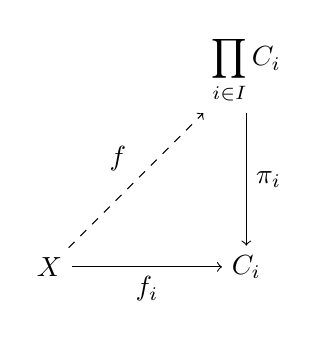
\begin{tikzpicture}[node distance=2.5cm, auto]
	\node (P) {$\displaystyle\prod_{i \in I} C_i$};
	\node (Ci) [below of=P] {$C_i$};
	\node (X) [left of=Ci] {$X$};
	\draw[->] (X) to node [swap] {$f_i$} (Ci);
	\draw[->, dashed] (X) to node {$f$} (P);
	\draw[->] (P) to node {$\pi_i$} (Ci);
\end{tikzpicture}
\end{figure}
\end{proposition}
\begin{proof}
Defina a função
	\begin{align*}
	\func{f}{X}{\prod_{i \in I} C_i}{x}{(f_i(x))_{i \in I}}.
	\end{align*}
Para todo $x \in X$ e para todo $i \in I$,
	\begin{equation*}
	\pi_i \circ f(x) = \pi_i (f(x)) = \pi_i ((f_i(x))_{i \in I}) = f_i(x).
	\end{equation*}
Portanto $\pi_i \circ f = f_i$. Isso mostra a existência da $f$. Para a unicidade, seja $\overline{f}: X \to \prod_{i \in I} C_i$ função tal que, para todo $i \in I$, $\pi_i \circ \overline{f} = f_i$. Seja $x \in X$.  Como $\overline{f}(x) \in \prod_{i \in I} C_i$, $\overline{f}(x) = (x_i)_{i \in I}$. Da propriedade comutativa de $\overline{f}$, segue que, para todo $i \in I$,
	\begin{equation*}
	x_i = \pi_i \circ \overline{f}(x) = f_i(x).
	\end{equation*}
Como $f(x) = (f_i(x))_{i \in I}$, isso mostra que $\overline{f}(x) = f(x)$. Portanto $\overline{f} = f$.
\end{proof}



%O axioma da escolha reescrito para famílias é o seguinte. Para toda família não vazia $(C_i)_{i \in I}$ de conjuntos (disjuntos) não vazios, existe uma função (\emph{função escolha}) $E: I \to \bigcup_{i \in I} C_i$ tal que, para todo $i \in I$, $E(i) \in C_i$.

%\begin{proposition}
%	Seja $(C_i)_{i \in I}$ uma família não vazia de conjuntos. Então
%	\begin{equation*}
%	\prod_{i \in I} C_i = \emptyset \qquad \Leftrightarrow \qquad \exists i \in I \quad C_i = \emptyset.
%	\end{equation*}
%\end{proposition}
%\begin{proof}
%	Primeiro, suponhamos que $(C_i)_{i \in I}$ é uma família de conjuntos não vazios. Então, pelo axioma da escolha, existe uma função $E: I \to \bigcup_{i \in I} C_i$ tal que, para todo $i \in I$, $E(i) \in C_i$. Assim, $E \in \prod_{i \in I} C_i$, o que mostra que $\prod_{i \in I} C_i \neq \emptyset$. Reciprocamente, suponhamos que existe alguma $i \in I$ tal que $C_i = \emptyset$. Então, se existisse $c \in \prod_{i \in I} C_i$, seguiria que $c(i) \in C_i = \emptyset$, o que é absurdo. Logo $\prod_{i \in I} C_i = \emptyset$.
%\end{proof}





\section{Coproduto de conjuntos}

\begin{definition}
Seja $(C_i)_{i \in I}$ uma família não vazia de conjuntos. O \emph{coproduto} de $(C_i)_{i \in I}$ é o conjunto
	\begin{equation*}
	\coprod_{i \in I} C_i :=\set{(i,c)}{i \in I \text{\ \ e\ \ } c \in C_i}.
	\end{equation*}
\end{definition}

\begin{definition}
Seja $(C_i)_{i \in I}$ uma família de conjuntos e $i \in I$. A \emph{inclusão canônica} de $C_i$ em $\coprod_{i \in I} C_i$ é a função
	\begin{align*}
	\func{\iota_i}{C_i}{\coprod_{i \in I} C_i}{c}{(i,c)}.
	\end{align*}
\end{definition}

\begin{proposition}[Propriedade Universal]
Sejam $(C_i)_{i \in I}$ uma família de conjuntos, $X$ um conjunto e, para todo $i \in I$, $f_i: C_i \to X$ uma função. Então existe uma única função $f: \coprod_{i \in I} C_i \to X$ tal que, para todo $i \in I$, $f \circ \iota_i = f_i$ (o diagrama comuta).
\begin{figure}
\centering
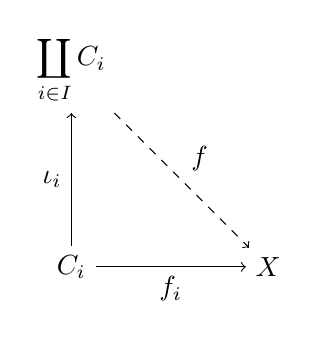
\begin{tikzpicture}[node distance=2.5cm, auto]
	\node (Ci) {$C_i$};
	\node (S) [above of=Ci] {$\displaystyle\coprod_{i \in I} C_i$};
	\node (X) [right of=Ci] {$X$};
	\draw[->] (Ci) to node [swap] {$f_i$} (X);
	\draw[->, dashed] (S) to node {$f$} (X);
	\draw[->] (Ci) to node {$\iota_i$} (S);
\end{tikzpicture}
\end{figure}
\end{proposition}
\begin{proof}
Defina a função
	\begin{align*}
	\func{f}{\coprod_{i \in I} C_i}{X}{(i,c)}{f_i(c)}.
	\end{align*}
Seja $i \in I$ e $c \in C_i$. Então
	\begin{equation*}
	f \circ \iota_i(c) = f(\iota_i(c)) = f(i,c) = f_i(c).
	\end{equation*}
Portanto $f \circ \iota_i = f_i$. Isso mostra a existência da $f$. Para a unicidade, seja $\overline{f}: \coprod_{i \in I} C_i \to X$ função tal que, para todo $i \in I$, $\overline{f} \circ \iota_i = f_i$. Seja $x \in \coprod_{i \in I} C_i$. Existem $i \in I$ e $c \in C_i$ tais que $x=(i,c)$. Da propriedade comutativa de $\overline{f}$, segue que
	\begin{equation*}
	\overline{f}(x) = \overline{f}(i,c) = \overline{f}(\iota_i(x)) = \overline{f} \circ \iota_i(c) = f_i(c) = f(i,c) = f(x).
	\end{equation*}
Isso mostra que $\overline{f}=f$.
\end{proof}


%\cleardoublepage
%\begin{figure}
%\centering
%\begin{tikzpicture}[node distance=4cm, auto]
%	\node (P) {$\displaystyle\prod_{i \in I} C_i$};
%	\node (Ci) [below of=P] {$C_i$};
%	\node (X) [left of=Ci] {$X$};
%	\node (S) [below of=Ci] {$\displaystyle\coprod_{i \in I} C_i$};
%	\node (Y) [right of=Ci] {$Y$};	
%	\draw[->] (X) to node [swap] {$f_i$} (Ci);
%	\draw[->, dashed] (X) to node {$f$} (P);
%	\draw[->] (P) to node {$\pi_i$} (Ci);
%	\draw[->] (Ci) to node {$g_i$} (Y);
%	\draw[->, dashed] (S) to node [swap] {$g$} (Y);
%	\draw[->] (Ci) to node [swap] {$\iota_i$} (S);
%\end{tikzpicture}
%\caption*{Os diagramas comutativos do \\produto e do coproduto de conjuntos.}
%\end{figure}





\cleardoublepage
\subsection{Propriedades de produto e coproduto}

\begin{proposition}
	Seja $(C_{ij})_{(i,j) \in I \times J}$ uma família de conjuntos. Então
	\begin{enumerate}
	\item $\displaystyle \bigcup_{j \in J} \left(\prod_{i \in I} C_{ij}\right) \subseteq \prod_{i \in I} \left(\bigcup_{j \in J} C_{ij}\right)$;
	\item $\displaystyle \bigcap_{j \in J} \left(\prod_{i \in I} C_{ij}\right) = \prod_{i \in I} \left(\bigcap_{j \in J} C_{ij}\right)$.
	\end{enumerate}
\end{proposition}
\begin{proof}
	\begin{enumerate}	
	\item \begin{align*}
	\displaystyle c \in  \bigcup_{j \in J} \left(\prod_{i \in I} C_{ij}\right)
		& \entao \exists j \in J \left(c \in \prod_{i \in I} C_{ij} \right) \\
		& \entao \exists j \in J \ \forall i \in I \left(c_i \in C_{ij} \right) \\
		& \entao \forall i \in I \left(c \in \bigcup_{j \in J} C_{ij} \right) \\
		& \entao  c \in \prod_{i \in I} \left(\bigcup_{j \in J} C_{ij}\right).
	\end{align*}
	
	\item 	
	\begin{align*}
	c \in \displaystyle \bigcap_{j \in J} \left(\prod_{i \in I} C_{ij}\right)
		& \sse \forall j \in J \left(c \in \prod_{i \in I} C_{ij} \right) \\
		& \sse \forall j \in J \ \forall i \in I \left(c_i \in C_{ij} \right) \\
		& \sse \forall i \in I \ \forall j \in J \left(c_i \in C_{ij} \right) \\
		& \sse \forall i \in I \left(c_i \in \bigcup_{j \in J} C_{ij} \right) \\
		& \sse  c \in \prod_{i \in I} \left(\bigcap_{j \in J} C_{ij}\right).
	\end{align*}
	\end{enumerate}
\end{proof}

Notemos que a inclusão contrária no primeiro item nao vale. Suponhamos que para um $j_0 \in J$, todos os $C_{ij_0}$ são vazios, mas para todos outros $j \in J$, os $C_{ij}$ não são vazios. Então o produto desses $C_{ij}$ será sempre vazio, pois sempre tem um dos elementos do produto vazio, e então a união desses produtos será vazia; no entanto, a união desses $C_{ij}$ não será nenhuma vazia e, então, o produto não seráa vazio (pelo axioma da escolha).

\begin{proposition}
\label{conj:proposition.im.inv.prod}
Sejam $X$ um conjunto, $(Y_i)_{i \in I}$ uma família de conjuntos, $(S_i)_{i \in I}$ uma família de subconjutos de $(Y_i)_{i \in I}$, $f: X \to \prod_{i \in I} Y_i$ uma função e, para todo $i \in I$, $f_i := \pi_i \circ f$. Então
	\begin{equation*}
	f\inv\left( \prod_{i \in I} {S_i} \right) = \bigcap_{i \in I} f_i\inv (S_i).
	\end{equation*}
\end{proposition}
\begin{proof}
Note que $x \in f\inv(\prod_{i \in I} {S_i})$ é equivalente a $f(x) \in \prod_{i \in I} {S_i}$, que por sua vez ocorre se, e somente se, para todo $i \in I$, $\pi_i(f(x)) \in S_i$. Como $f_i(x)=\pi_i(f(x)) \in S_i$, isso é equivalente a, para todo $i \in I$, $x \in f_i\inv (S_i)$.
\end{proof}





%\begin{definition}
%Seja $C$ um conjunto não vazio. A \emph{soma} de $C$ é o conjunto
%	\begin{equation*}
%	\coprod C := \set{(X,x) \in C \times \bigcup C}{x \in X}.
%	\end{equation*}
%\end{definition}

%Vale notar que a soma de $C$ existe porque é um subconjunto de $\p\left(C \times \bigcup C \right)$, logo é um conjunto pelo axioma da especificação.

%Definimos a seguir uma nova operação em uma família $(C_i)_{i \in I}$, a soma, também chamada de união disjunta. Em vez de unirmos todos elementos de $(C_i)_{i \in I}$, indexamos cada um deles com o índice do conjunto da família a que ele pertence para que, se um mesmo elemento, digamos $c$, pertencer $C_{i_1}$ e $C_{i_2}$, $i_1,i_2 \in I$ distintos, então na união disjunta $(c,i_1)$ e $(c,i_2)$ serão elementos distintos, enquanto que na união não haverá distinção.



%\begin{conjectura}
%	Seja $(C_i)_{i \in I}$ uma família não vazia de conjuntos. Então
%	\begin{equation*}
%	\coprod_{i \in I} C_i = \emptyset \qquad \Leftrightarrow \qquad \forall i \in I \quad C_i = \emptyset.
%	\end{equation*}
%\end{conjectura}


\subsubsection*{Notação alternativa}

\begin{equation*}
\prod_{i \in I} C_i = \set{\lceil c_i \rceil_{i \in I}}{\forall i \in I \; c_i \in C_i}
\end{equation*}

$\lceil c_i \rceil_{i \in I} = c: I \to \bigcup_{i \in I} C_i$

\begin{equation*}
\coprod_{i \in I} C_i = \set{\lfloor c \rfloor_i}{i \in I, c \in C_i}
\end{equation*}

$\lfloor c \rfloor_i = (i,c)$




\section{Complementares e diferença simétrica}

\begin{definition}
Sejam $X$ e $Y$ conjuntos. O \emph{complementar relativo} de $Y$ em $X$ é o conjunto
	\begin{equation*}
	X \setminus Y := \set{x \in X}{x \notin Y}.
	\end{equation*}
\end{definition}

\begin{definition}
Sejam $X$ um conjunto e $S$ um subconjunto de $X$. O \emph{complementar} de $S$ em $X$ é o conjunto
	\begin{equation*}
	S^\complement := X \setminus S.
	\end{equation*}
%Seja $\mathcal A \subseteq \p(A)$. O \emph{conjunto complementar} de $\mathcal A$ em $A$ é o conjunto
%	\begin{equation*}
%	\complementlement(\mathcal A) := \{X^\complement : X \in \mathcal A\}.
%	\end{equation*}
\end{definition}

\begin{definition}
Sejam $X$ e $Y$ conjuntos. A \emph{diferença simétrica} de $X$ e $Y$ é o conjunto
	\begin{equation*}
	X \difsim Y := (X \setminus Y) \cup (Y \setminus X).
	\end{equation*}
\end{definition}

\subsection{Propriedades}

\begin{proposition}
Sejam $X$, $Y$ subconjuntos de $U$. Então
	\begin{enumerate}
	\item $(X^\complement)^\complement = X$;
	\item $\emptyset^\complement = U$ e $U^\complement = \emptyset$;
	\item $X \cap X^\complement = \emptyset$ e $X \cup X^\complement = U$;
	\item $X \subseteq Y \sse Y^\complement \subseteq X^\complement$.
	\item $(X \cup Y)^\complement = X^\complement \cap Y^\complement$ e $(X \cap Y)^\complement = X^\complement \cup Y^\complement$.
	\end{enumerate}
\end{proposition}




\section{Coberturas e partições}

\begin{definition}
Seja $X$ um conjunto. Uma \emph{cobertura} de $X$ é uma família $(C_i)_{i \in I}$ de subconjuntos de $X$ cuja união é $X$:
	\begin{equation*}
	\bigcup_{i \in I} C_i = X.
	\end{equation*}
Um \emph{subcobertura} de uma cobertura $(C_i)_{i \in I}$ de $X$ é uma cobertura $(C_i)_{i \in J}$ de $X$, com $J \subseteq I$.
\end{definition}

\begin{definition}
Seja $X$ um conjunto. Uma \emph{partição} de $X$ é um conjunto $\mathcal P \subseteq \p(X)$ de subconjuntos de $X$ que satisfaz
	\begin{enumerate}
	\item $\emptyset \notin \mathcal P$;
	\item $\displaystyle\bigcup \mathcal P = X$;
	\item Para todos conjuntos distintos $C_0,C_1 \in \mathcal P$, $C_0 \cap C_1 = \emptyset$.
	\end{enumerate}
Os conjuntos $C \in \mathcal P$ são as \emph{células} de $\mathcal P$.
\end{definition}

Uma partição, se identidicamos um subconjunto de $\p(X)$ com uma família de sunconjuntos de $X$, é uma cobertura de $X$ por conjuntos disjuntos (logo distintos) que não contém o conjunto vazio.

\subsection{Refinamento de partições}

\begin{definition}
Sejam $X$ um conjunto e $\mathcal P$ uma partição de $X$. Um \emph{refinamento} (\emph{superpartição}) de $\mathcal P$ é uma partição $\mathcal R$ de $X$ que satisfaz: para toda célula $D \in \mathcal R$, existe uma célula $C \in \mathcal P$ tal que $D \subseteq C$. Denota-se $\mathcal P \leq \mathcal R$. Diz que $\mathcal P$ é um \emph{engrossamento} (\emph{subpartição}) de $\mathcal R$.
\end{definition}

\begin{proposition}
Sejam $X$ um conjunto e $\mathcal P,\mathcal R$ partições de $X$ tais que $\mathcal P \leq \mathcal R$. Então
	\begin{enumerate}
	\item $\card{\mathcal P} \leq \card{\mathcal R}$;
	\item Para cada célula $C \in \mathcal P$, o conjunto
		\begin{equation*}
		\mathcal R|_C := \set{D \in \mathcal R}{D \subseteq C}
		\end{equation*}
é uma partição de $C$.
	\end{enumerate}
\end{proposition}
\begin{proof}
	\begin{enumerate}
	\item Por definição de refinamento, para toda célula $D \in \mathcal R$ existe célula $C \in \mathcal P$ tal que $D \subseteq C$. Notemos que essa célula $C$ é única pois, se existir célula $C' \in \mathcal P$ tal que $D \subseteq C'$, então $D \subseteq C \cap C'$ e, como $D \neq \emptyset$, segue que $C =C'$. Assim, consideramos a função que mapeia, para cada célula $D \in \mathcal R$ a célula $C_D \in \mathcal P$ tal que $D \subseteq C_D$:
	\begin{align*}
	\func{f}{\mathcal R}{\mathcal P}{D}{C_D}.
	\end{align*}
Mostremos que essa função é sobrejetiva. Para isso, seja $C \in \mathcal P$. Como $\bigcup \mathcal R = X$, para todo $x \in C \subseteq X$ existe $D \in \mathcal R$ tal que $x \in D$. Como $C \neq \emptyset$, existe $x \in C$, logo existe $D \in \mathcal R$ tal que $x \in D$. Por definição de refinamento, existe $C' \in \mathcal P$ tal que $D \subseteq C'$, o que implica $x \in C'$. Como $x \in C' \cap C$, segue que $C=C'$, e concluímos que $D \subseteq C$. Isso mostra que $f(D)=C$, logo que $f$ é sobrejetiva. Concluímos, então, que $\card{\mathcal P} \leq \card{\mathcal R}$.
	
	\item As propriedades 1 e 3 são evidentes por que $\mathcal R$ é partição. Para a propriedade 2, seja $C \in \mathcal P$ e $U := \bigcup \set{D \in \mathcal R}{D \subseteq C}$. Notemos que $C=U$. Para mostrar isso, seja $x \in C$. Então existe $D \in \mathcal R$ tal que $x \in D$, pois $\bigcup \mathcal P=X$. Por definição de refinamento, existe $C' \in \mathcal P$ tal que $D \subseteq C'$, portanto $x \in C'$. Como $x \in C' \cap C$, segue que $C=C'$. concluímos que $D \subseteq C$, portanto que $x \in U$, o que mostra $C \subseteq U$. Reciprocamente, para todo $D \in U$, $D \subseteq C$, portanto $U \subseteq C$, e concluímos que $C=U$.
	\end{enumerate}
\end{proof}

\begin{proposition}
Sejam $X$ um conjunto. A relação de refinamento $\leq$ no conjunto de partições de $X$ é uma relação de ordem parcial.
\end{proposition}

\begin{definition}
Sejam $X$ um conjunto e $(\mathcal P_i)_{i \in I}$ uma família de partições de $X$. O \emph{refinamento comum} a $(\mathcal P_i)_{i \in I}$ é o conjunto
	\begin{equation*}
	\bigvee_{i \in I} \mathcal P_i := \set{\bigcap_{i \in I} C_i}{i \in I,\  C_i \in \mathcal P_i \text{\ \ e\ \ } \bigcap_{i \in I} C_i \neq \emptyset}.
	\end{equation*}
\end{definition}

\begin{proposition}
Sejam $X$ um conjunto e $(\mathcal P_i){i \in I}$ uma família de partições de $X$. O refinamento comum $\bigvee_{i \in I} \mathcal P_i$ a $(\mathcal P_i)_{i \in I}$ é a menor partição de que $X$ que refina $\mathcal P_i$ para todo $i \in I$.
\end{proposition}
\begin{proof}
Primeiro, mostremos que $\mathcal P := \bigvee_{i \in I} \mathcal P_i$ é uma partição. Por definição, $\emptyset \notin \mathcal P$. Seja $x \in X$. Então, para cada $i \in I$, existe $C_i \in \mathcal P_i$ tal que $x \in C_i$, pois $\bigcup \mathcal P_i = X$. Sendo assim, $x \in \bigcap_{i \in I} C_i$, portanto $X \subseteq \bigcup \mathcal P$, e segue que $\bigcup \mathcal P = X$. Por fim, sejam $C=\bigcap_{i \in I} C_i, D=\bigcap_{i \in I} D_i \in \mathcal P$. Se $C \neq D$, então existe $x \in C\setminus D$ ou existe $x \in D \setminus C$. Sem perda de generalidade, suponha o primeiro. Então, existe $i \in I$ tal que $x \notin D_i$. Como $x \in C$, então $x \in C_i$, portanto $C_i \neq D_i$. Mas então, como $\mathcal P_i$ é partição, $C_i \cap D_i = \emptyset$. Por fim, como $C \subseteq C_i$ e $D \subseteq D_i$, segue que $C \cap D = \emptyset$.

Agora mostraremos que $\mathcal P$ é refinamento de $\mathcal P_i$ para todo $i \in I$. Sejam $i \in I$ e $C \in \mathcal P$. Então $\mathcal P=\bigcap_{i \in I} C_i$, portanto $C_i \in \mathcal P_i$. Por fim, sejam $\mathcal R$ partição de $X$ que é refina $\mathcal P_i$ para todo $i \in I$ e $D \in \mathcal R$ uma célula. Então, para todo $i \in I$, existe $C_i \in \mathcal P_i$ tal que $D \subseteq C_i$. Portanto $D \subseteq \bigcap_{i \in I} C_i$, e como $\bigcap_{i \in I} C_i \in \mathcal P$, segue que $\mathcal P \leq \mathcal R$.
\end{proof}

Alguns tipos especiais de partições são úteis na teoria de intergação de Riemmann. Em $\R^1$, essas partições são chamadas de partições de intervalo, e são representadas como um número finito de pontos em um intervalo. Quando generaliza-se para dimensões maiores, usam-se $n$-retângulos, que são conjuntos em $\R^n$ produtos de $n$ intervalos limitados. Podemos fixar um critério a mais, o de que um $n$-retângulo é produto de intervalos fechados em baixo e abertos em cima. Nesse caso, podemos definir que uma partição cujos elementos são $n$-retângulos é uma \emph{malha}.

Alternativamente, quando temos uma medida, que é o caso de $\R^n$, podemos enfraquecer a restrição de que as células de uma partição são iguais ou disjuntas para a de que são iguais ou \emph{quase disjuntas} \--- a interseção tem medida zero \--- e a restrição de que cobrem para a restrição de que a união da partição é quase total \--- seu complementar tem medida nula \--- e por fim, de que nenhum elemento da partição é quase vazio \--- tem medida nula \--- e definir que isso é uma $\mu$-partição ou \emph{quase partição com respeito a $\mu$}.
\chapter{Relações}

Definimos brevemente o que são relações e, em especial, relações binárias, antes de abordar os casos específicos de funções, equivalências e ordens.

\begin{definition}
Sejam $X$ e $Y$ conjuntos. Uma \emph{relação} $R$ de $X$ para $Y$ é um subconjunto de $X \times Y$. Os conjuntos $X$ e $Y$ são, respectivamente, o \emph{domínio} e o \emph{contradomínio} de $R$. Denota-se $x \mathrel{R} y$ para $(x,y) \in R$.
\end{definition}

\begin{definition}
	Seja $A$ um conjunto não vazio. Uma \emph{relação binária} $R$ em $A$ é uma relação $R$ de $A$ para $A$.
\end{definition}

\begin{definition}
	Seja $A$ um conjunto não vazio e $R$ uma relação binária em $A$. Definem-se as seguintes propriedades de $R$:
	\begin{enumerate}
	\item (Reflexividade) $\forall a \in A \qquad aRa$;
	\item (Irreflexividade) $\nexists a \in A \qquad aRa$;
	\item (Simetria) $\forall a_1,a_2 \in A \qquad a_1Ra_2 \Leftrightarrow a_2Ra_1$;
	\item (Antissimetria) $\forall a_1,a_2 \in A \qquad a_1Ra_2 \text{\ \ e\ \ } a_2Ra_1 \Rightarrow a_1=a_2$;
	\item (Transitividade) $\forall a_1,a_2,a_3 \in A \qquad a_1Ra_2 \text{\ \ e\ \ } a_2Ra_3 \Rightarrow a_1Ra_3$;
	\item (Totalidade) $\forall a_1,a_2 \in A \qquad a_1Ra_2 \text{\ \ ou\ \ } a_2Ra_1$.
	\end{enumerate}
	Uma relação que satisfaz as propriedades acima é, respectivamente, reflexiva, simétrica, antissimétrica, transitiva e total.
\end{definition}

\section{Funções}

\begin{definition}
Seja $R$ uma relação de $X$ em $Y$. A \emph{relação inversa} de $R$ é a relação $R\inv$ de $Y$ em $X$ definida por
	\begin{equation*}
	\forall x \in X\ \forall y \in Y \qquad x \mathrel{R} y \Leftrightarrow y \mathrel{R\inv} x.
	\end{equation*}
\end{definition}


\subsection{Definição e propriedades básicas}

\begin{definition}
Sejam $A$ e $B$ conjuntos. Uma \emph{função} de $A$ para $B$ é uma relação $f$ de $A$ para $B$ tal que
	\begin{enumerate}
		\item (Funtorialidade) Para todo $a \in A$, existe único $b \in B$ tal que $(a,b) \in f$.
	\end{enumerate}
Denota-se $f: A \to B$. O conjunto das funções de $A$ para $B$ é denotado $\Func(A,B)$ ou $B^A$. O conjunto das funções de $A$ para $A$ é denotado $\Func(A)$.

A \emph{imagem} de $a \in A$ é o único $b \in B$ que satisfaz $(a,b) \in f$. Denota-se $b=f(a)$. Ambas informações podem ser denotadas por
	\begin{align*}
	\func{f}{A}{B}{a}{b}.
	\end{align*}

\end{definition}

\begin{proposition}
Seja $f: A \to B$ uma função. Então
	\begin{enumerate}
	\item $A=\emptyset \sse f=\emptyset$.
	\item $B=\emptyset \entao A=\emptyset$.
	\end{enumerate}
\end{proposition}
\begin{proof}
	\begin{enumerate}
	\item Suponhamos que $A=\emptyset$. Primeiro, notemos que $f=\emptyset$ é uma função de $\emptyset$ em $B$. Claramente, $f = \emptyset \subseteq \emptyset \times B$. Ainda, se $f$ não fosse função de $\emptyset$ em $B$, existiria $a \in \emptyset$ tal que não existe único $b \in B$ satisfazendo $(a,b) \in f$. Mas existir $a \in \emptyset$ é uma contradição. Logo $f$ é função. Por fim, se $g: \emptyset \times B$ é uma função, como $\emptyset \times B = \emptyset$, então $g \subseteq \emptyset \times B = \emptyset$, logo $g=\emptyset=f$.
	
Reciprocamente, suponhamos $f=\emptyset$. Se $A \neq \emptyset$, seja $a \in A$. Como $f$ é função, existe $b \in B$ tal que $(a,b) \in f=\emptyset$, o que é contradição. Portanto $A=\emptyset$.
	
	\item Suponhamos que $A \neq \emptyset$. Então existe $a \in A$ e, como $f$ é função, existe único $b \in \emptyset$ tal que $(a,b) \in f$. Mas $b \in \emptyset$ é absurdo, o que mostra que $A = \emptyset$.
	\end{enumerate}
\end{proof}

\begin{proposition}\label{conj:prop.func.ig}
Sejam $f: A \to B$ e $g:A' \to B'$. Então
	\begin{equation*}
	f=g \sse A=A' \e \forall a \in A \quad f(a)=g(a).
	\end{equation*}
\end{proposition}
\begin{proof}
Suponhamos que $f=g$. Se $A=\emptyset$, então $f=\emptyset$ e $g=f=\emptyset$, o que implica $A'=\emptyset$. Ainda, para todo $a \in A$, $f(a)=g(a)$ pois, se isso fosse falso, existiria $a \in \emptyset$ tal que $f(a)\neq g(a)$, mas existir $a \in \emptyset$ é absurdo. Se $A \neq \emptyset$, seja $a \in A$. Então existe $b \in B$ tal que $(a,b) \in f$ e, como $f=g$, $(a,b) \in g$. Isso implica $a \in A'$ e concluímos que $A \subseteq A'$. Por outro lado, seja $a \in A'$. Então existe $b \in B'$ tal que $(a,b) \in g$ e, como $f=g$, $(a,b) \in f$. Isso implica $a \in A$ e concluímos que $A' \subseteq A$. Portanto $A=A'$. Agora, seja $a \in A$. Então existem $f(a) \in B$ e $g(a) \in B'$. Como $(a,f(a)) \in f$ e $f=g$, então $(a,f(a)) \in g$. Como $f$ é função, existe único $b \in B$ tal que $(a,b) \in f$, o que implica $f(a)=g(a)$.
	
Reciprocamente, suponhamos que $A=A'$ e que, para todo $a \in A$, $f(a)=g(a)$. Se $A=\emptyset$, então $f=\emptyset$ e $g=\emptyset$, logo $f=g$. Se $A \neq \emptyset$, então seja $p \in f$. Existe $a \in A$ tal que $p=(a,f(a))$. Como $f(a)=g(a)$, então $p=(a,g(a))$; mas $(a,g(a)) \in g$, o que implica $p \in g$ e, portanto, $f \subseteq g$. Agora, seja $p \in g$. Existe $a \in A'$ tal que $p=(a,g(a))$. Como $f(a)=g(a)$, então $p=(a,f(a))$; mas $(a,f(a)) \in f$, o que implica $p \in f$ e, portanto, $f \subseteq g$. Assim, concluímos que $f=g$.
\end{proof}

\begin{definition}
Sejam $f: A \to B$ uma função e $C \subseteq A$ um conjunto. O \emph{conjunto imagem} de $C$ sob $f$ é
	\begin{equation*}
	f(C)=\set{y \in Y}{\exists c \in C \quad y=f(c)}.
	\end{equation*}
O conjunto $f(A)$ é o \emph{imagem} de $f$.
\end{definition}

\begin{proposition}
Seja $f: A \to B$. Então $f: A \to f(A)$.
\end{proposition}

\begin{definition}
Sejam $f: A \to B$ uma função e $A' \subseteq A$ um conjunto. A \emph{restrição} de $f$ a $A'$ é a função
	\begin{align*}
	\func{f|_{A'}}{A'}{B}{a}{f(a)}.
	\end{align*}
\end{definition}

\begin{proposition}\label{conj:prop.func.rest.ig}
	Sejam $f: A \to B$, $A' \subseteq A$ e $B' \subseteq B$. Então a restrição $f|_{A'}$ é uma função de $A'$ em $B'$ se, e somente se, $f(A') \subseteq B'$.
\end{proposition}
\begin{proof}
	Se que $f|_{A'}$ é uma função de $A'$ em $B'$, então o contradomínio de $f_{A'}$ é $B'$, o que significa que, para todo $a \in A'$, $f(a) = f|_{A'}(a) \in B'$, logo $f(A') \subseteq B$. Reciprocamente, se, para todo $a \in A'$, $f(a) \in B'$, então $f|_{A'}$ é uma função de $A'$ em $B'$.
\end{proof}

\subsection{Composição de funções}

\begin{definition}
	Sejam $f: A \to B'$ e $g: B \to C$ funções tais que $B' \subseteq B$. A \emph{função composta} de $g$ com $f$ é a função
	\begin{align*}
	\func{g \circ f }{A}{C}{a}{g(f(a))}.
	\end{align*}
\end{definition}

\begin{proposition}
\label{prop:comp.func.asso}
	Sejam $f: A \to B'$, $g: B \to C'$ e $h: C \to D$ funções tais que $B' \subseteq B$ e $C' \subseteq C$. Então
	\begin{equation*}
	h \circ (g \circ f) = (h \circ g) \circ f.
	\end{equation*}
\end{proposition}
\begin{proof}
	Primeiro, notemos que $g \circ f$ é uma função de $A$ em $C'$, o que implica que $h \circ (g \circ f)$ é uma função de $A$ em $D$. Anda, notemos que $h \circ g$ é uma função de $B$ em $D$, o que implica que $(h \circ g) \circ f$ é uma função de $A$ em $D$. Logo os domínios de $h \circ (g \circ f)$ e $(h \circ g) \circ f$ são iguais. Se $A=\emptyset$, então $h \circ (g \circ f) = (h \circ g) \circ f = \emptyset$. Suponhamos, então, que $A \neq \emptyset$ e seja $a \in A$. Então
	\begin{equation*}
	(h \circ (g \circ f))(a) = h((g \circ f)(a)) = h(g(f(a))) = (h \circ g)(f(a)) = ((h \circ g) \circ f)(a),
	\end{equation*}
o que mostra que $h \circ (g \circ f) = (h \circ g) \circ f$. 
\end{proof}

\begin{proposition}
	Seja $f\colon A \to B$. Então
	\begin{enumerate}
	\item $f \circ \emptyset = \emptyset$;
	\item $\emptyset \circ f = \emptyset$.
	\end{enumerate}
\end{proposition}
\begin{proof}
	Para a primeira igualdade, notemos que $f \circ \emptyset$ é uma função de $\emptyset$ em $B$ e, portanto, $f \circ \emptyset=\emptyset$. Para a segunda igualdade, notemos que $\emptyset \circ f$ é uma função de $A$ em $\emptyset$ e, portanto, $A=\emptyset$, o que é equivalente a $\emptyset \circ f=\emptyset$.
\end{proof}

\begin{definition}
	Seja $A$ um conjunto não vazio. A \emph{função identidade} em $A$ é a função
	\begin{align*}
	\func{\Id_A}{A}{A}{a}{a}.
	\end{align*}
\end{definition}

\begin{proposition}
\label{prop:id.comp.func}
	Seja $f\colon A \to B$ uma função. Então
	\begin{equation*}
	f \circ \Id_A = f \e \Id_B \circ f = f.
	\end{equation*}
\end{proposition}
\begin{proof}
	Primeiro, notemos que $f \circ \Id_A$ e $\Id_B \circ f$ são funções de $A$ em $B$ e, portanto, têm o mesmo domínio de $f$. Se $A = \emptyset$, então $f: \emptyset \to B$ e, portanto, $f=\emptyset$. Notemos que $\Id_\emptyset = \emptyset$. De fato, $\emptyset$ é função e, se não fosse identidade de $\emptyset$ em $\emptyset$, existiria $a \in \emptyset$ tal que $f(a) \neq a$; mas $a \in \emptyset$ é absurdo. Assim, $f \circ \Id_A$ é uma função de $\emptyset$ em $B$ e, portanto, $f \circ \Id_A = \emptyset = f$. Ainda, $\Id_B \circ f$ é uma função de $\emptyset$ em $B$ e, portanto, $\Id_B \circ f = \emptyset = f$. Se $A \neq \emptyset$, seja $a \in A$. Então $(f \circ \Id_A) (a) = f(\Id_A(a)) = f(a) = \Id_B(f(a)) = (\Id_B \circ f)(a)$.
\end{proof}

\subsection{Função inversa, injetividade e sobrejetividade}

\begin{definition}
Seja $f\colon A \to B$ uma função. Uma \emph{função inversa} de $f$ é uma função $g\colon B \to A$ tal que
	\begin{equation*}
	g \circ f = \Id_A \e f \circ g = \Id_B.
	\end{equation*}
\end{definition}

\begin{definition}
Uma \emph{função injetiva} (ou \emph{injeção}) é uma função $f\colon A \to B$ que satisfaz
	\begin{equation*}
	\forall a_1,a_2 \in A \qquad f(a_1)=f(a_2) \Rightarrow a_1=a_2.
	\end{equation*}
O conjunto das funções injetivas de $A$ para $B$ é denotado $\Mono{\Func}(A,B)$. O conjunto das funções injetivas de $A$ para $A$ é denotado $\Mono{\Func}(A)$.
\end{definition}

\begin{definition}
Uma \emph{função sobrejetiva} sobre um conjunto $B$ é uma função $f\colon A \to B$ que satisfaz $f(A)=B$. O conjunto das funções sobrejetivas de $A$ para $B$ é denotado $\Epi{\Func}(A,B)$. O conjunto das funções sobrejetivas de $A$ para $A$ é denotado $\Epi{\Func}(A)$.
\end{definition}

\begin{definition}
Sejam $A$ e $B$ conjunto. Uma \emph{bijeção} entre $A$ e $B$ é uma função injetiva $f\colon A \to B$ que é sobrejetiva sobre $B$. O conjunto das funções bijetivas de $A$ para $B$ é denotado $\Iso{\Func}(A,B)$.
\end{definition}

\begin{proposition}
\label{prop:func.inv.esq}
Seja $f\colon A \to B$. Então $f$ é injetiva se, e somente se, existe $g\colon B \to A$ tal que $g \circ f = \Id_A$.
\end{proposition}
\begin{proof}
Suponhamos que $f$ é injetiva. Se $A = \emptyset$. Então $f=\emptyset$ e, portanto, tomando $g=\Id_B$, temos que $g \circ f = \Id_B \circ \emptyset = \Id_\emptyset = \emptyset$.
	Se $A \neq \emptyset$, seja $a \in A$.
	
	
\end{proof}

\begin{proposition}
\label{prop:func.inv.dir}
Seja $f\colon A \to B$. Então $f$ é sobrejetiva sobre $B$ se, e somente se, existe $g\colon B \to A$ tal que $f \circ g = \Id_B$.
\end{proposition}
\begin{proof}
Suponhamos que $f$ é sobrejetiva sobre $B$. Então $B=f(A)$; ou seja, para todo $b \in B$, existe $a \in A$ tal que $f(a)=b$ e, portanto, definimos a função $g\colon B \to A$ para cada elemento de $B$ como $g(b) := a$. Assim, segue que $g \circ f = \Id_B$.
\end{proof}

\begin{proposition}
	Seja $f\colon A \to B$. Se $g\colon B \to A$ e $g'\colon B \to A$ são funções inversas de $f$, então $g=g'$.
\end{proposition}
%\begin{proof}
%	Primeiro, notemos que os domínios de $g$ e $g'$ são os mesmos. Agora, se $A=\emptyset$, então $f=\emptyset$. Mas isso significa que $\Id_A = \emptyset$ e, como $g$ e $g'$ são inversas de $f$, segue que $g$
%	 (NÃO SEI SE ROLA COM A=0).
	
%	Se $A \neq \emptyset$, seja $a \in A$. Então $g \circ f = \Id_B$
%\end{proof}

\begin{proposition}
\label{prop:comp.func.inj}
	Sejam $f\colon A \to B'$ e $g\colon B \to C$ funções tais que $B' \subseteq B$. Se $f$ e $g$ são funções injetivas, então $g \circ f$ é uma função injetiva.
\end{proposition}
\begin{proof}
	Sejam $a_1,a_2 \in A$ tais que $g \circ f(a_1)=g \circ f(a_2)$. Então $g(f(a_1))=g(f(a_2))$. Como $g$ é injetiva, então $f(a_1)=f(a_2)$ e, como $f$ é injetiva, então $a_1=a_2$. Portanto $g \circ f$ é injetiva.
\end{proof}

\begin{proposition}
\label{prop:comp.func.sobr}
	Sejam $f\colon A \to B$ e $g\colon B \to C$ funções. Se $f$ e $g$ são funções sobrejetivas, então $g \circ f$ é uma função sobrejetiva.
\end{proposition}
\begin{proof}
	Como $f$ é sobrejetiva, então $f(A)=B$. Ainda, como $g$ é sobrejetiva, então $g(B)=C$. Então $g \circ f(A) = g(f(A))=g(B)=C$. Portanto $g \circ f$ é sobrejetiva.
\end{proof}

\subsection{Imagem inversa de função e propriedades}

\begin{definition}
	Seja $f: A \to B$ uma função e $B' \subseteq B$. A \emph{imagem inversa} de $B$ sob $f$ é o conjunto
	\begin{equation*}
	f^{-1}(B') := \set{a \in A}{f(a) \in B'}.
	\end{equation*}
\end{definition}

\begin{proposition}
\label{prop:props.imag.inv}
	Seja $f: A \to B$ uma função, $B' \subseteq B$ e $(B_i)_{i \in I} \subseteq \p(B)$ uma família de subconjuntos de $B$. Então
	\begin{enumerate}
	\item $f^{-1}(\emptyset) = \emptyset$;
	\item $f^{-1}(B) = A$;
	\item $f^{-1}\left((B')^\complement\right) = (f^{-1}(B'))^\complement$;
	\item $f^{-1}\left(\displaystyle\bigcup_{i \in I} B_i\right) = \displaystyle\bigcup_{i \in I} f^{-1}(B_i)$;
	\item $f^{-1}\left(\displaystyle\bigcap_{i \in I} B_i\right) = \displaystyle\bigcap_{i \in I} f^{-1}(B_i)$.
	\end{enumerate}
\end{proposition}
\begin{proof}
	\begin{enumerate}
	\item Suponha, por absudo, que existe $a \in f^{-1}(\emptyset)$. Então $f(a) \in \emptyset$, o que é absurdo, e conclui-se $f^{-1}(\emptyset) = \emptyset$.
	\item Seja $a \in A$. Como f é função de $A$ em $B$, então existe $b \in B$ tal que $f(a)=b$, o que implica $a \in f^{-1}(B)$ e, então, $a \subseteq A$. Como a inclusão contrária vale por definição, então$f^{-1}(B) = A$.
	\item Seja $a \in f^{-1}((B')^\complement)$. Então $f(a) \in (B')^\complement$. Mas isso implica $a \notin f^{-1}(B')$, pois, caso contrário, seguiria que $f(a) \in B'$, o que contradiz a hipótese. Portanto $a \in (f^{-1}(B'))^\complement$; ou seja, $f^{-1}((B')^\complement) \subseteq (f^{-1}(B'))^\complement$. Reciprocamente, seja $a \in (f^{-1}(B'))^\complement$. Se, por absurdo, $f(a) \in B'$, então $a \notin f^{-1}(B')$, o que contradiz a hipótese. Portanto $f(a) \in (B')^\complement$, o que implica $a \in f^{-1}((B')^\complement)$. Assim conclui-se que $(f^{-1}(B'))^\complement \subseteq f^{-1}((B')^\complement)$ e, portanto, $f^{-1}((B')^\complement) = (f^{-1}(B'))^\complement$.
	\item Seja $a \in f^{-1}(\bigcup_{i \in I} B_i)$. Então $f(a) \in \bigcup_{i \in I} B_i$. Isso significa que exite $i \in I$ tal que $f(a) \in B_i$. Portanto $a \in f^{-1}(B_i)$, e segue que $a \in \bigcup_{i \in I} f^{-1}(B_i)$; ou seja, $f^{-1}(\bigcup_{i \in I} B_i) \subseteq \bigcup_{i \in I} f^{-1}(B_i)$. Reciprocamente, seja $a \in \bigcup_{i \in I} f^{-1}(B_i)$. Então existe $i \in I$ tal que $a \in f^{-1}(B_i)$. Então $f(a) \in B_i$. Mas isso implica que $f(a) \in \bigcup_{i \in I} B_i$. Portanto $a \in f^{-1}(\bigcup_{i \in I} B_i)$; ou seja, $\bigcup_{i \in I} f^{-1}(B_i) \subseteq f^{-1}(\bigcup_{i \in I} B_i)$. Assim, conclui-se que $f^{-1}(\bigcup_{i \in I} B_i) = \bigcup_{i \in I} f^{-1}(B_i)$.
	\item Seja $a \in f^{-1}(\bigcap_{i \in I} B_i)$. Então $f(a) \in \bigcap_{i \in I} B_i$. Isso significa que, para todo $i \in I$, $f(a) \in B_i$. Portanto, para todo $i \in I$, $a \in f^{-1}(B_i)$, e segue que $a \in \bigcap_{i \in I} f^{-1}(B_i)$; ou seja, $f^{-1}(\bigcap_{i \in I} B_i) \subseteq \bigcap_{i \in I} f^{-1}(B_i)$. Reciprocamente, seja $a \in \bigcap_{i \in I} f^{-1}(B_i)$. Então, para todo $i \in I$, $a \in f^{-1}(B_i)$. Então, para todo $i \in I$, $f(a) \in B_i$, o que implica que $f(a) \in \bigcap_{i \in I} B_i$. Portanto $a \in f^{-1}(\bigcap_{i \in I} B_i)$; ou seja, $\bigcap_{i \in I} f^{-1}(B_i) \subseteq f^{-1}(\bigcap_{i \in I} B_i)$. Assim, conclui-se que $f^{-1}(\bigcap_{i \in I} B_i) = \bigcap_{i \in I} f^{-1}(B_i)$.
\qedhere
	\end{enumerate}
\end{proof}

\subsection{Propriedades de imagem e imagem inversa}

\begin{proposition}
	Sejam $f: D \to C$ uma função e $(C_i)_{i \in I}$ uma família de subconjuntos de $C$. Então
	\begin{enumerate}
	\item $f(\emptyset) = \emptyset$;
	\item $f(D) \subseteq C$;
	\item $f\left(\displaystyle\bigcup_{i \in I} C_i \right) = \displaystyle\bigcup_{i \in I} f(C_i)$;
	\end{enumerate}
\end{proposition}
\begin{proof}
	\begin{enumerate}
	\item Suponha, por absurdo, que existe $c \in f(\emptyset)$. Nesse caso, existe $d \in \emptyset$ tal que $f(d) = c$, o que é absurdo. Logo $f(\emptyset) = \emptyset$.
	\item Se$f(D)=\emptyset$, então vale a proposição. Caso contrário, seja $c \in f(D)$. Então existe $d \in D$ tal que $f(d)=c \in C$.
	\item Se $f \left( \bigcup_{i \in I} C_i \right) = \emptyset$, então $\bigcup_{i \in I} C_i = \emptyset$. Assim, segue que, para todo $i \in I$, $C_i = \emptyset$ e temos que $f(C_i)=\emptyset$. Portanto $\bigcup_{i \in I} f(C_i) = \emptyset$. Caso contrário, seja $d \in f \left( \bigcup_{i \in I} C_i \right)$. Então existe $c \in \bigcup_{i \in I} C_i$ tal que $f(c)=d$ e, consequentemente, existe $i \in I$ tal que $c \in C_i$. Assim, segue que $d=f(c) \in f(C_i) \subseteq \bigcup_{i \in I} f(C_i)$.
	
	Reciprocamente, se $\bigcup_{i \in I} f(C_i) = \emptyset$, então, para todo $i \in I$, $f(C_i) = \emptyset$, o que implica $C_i = \emptyset$. Assim, segue que $\bigcup_{i \in I} C_i = \emptyset$ e, portanto, $f\left(\bigcup_{i \in I} C_i \right) = \emptyset$. Caso contrário, seja $d \in \bigcup_{i \in I} f(C_i)$. Então existe $i \in I$ tal que $d \in f(C_i)$ e, consequentemente, existe $c \in C_i$ tal que $f(c)=d$. Assim, segue que $c \in \bigcup_{i \in I} C_i$ e, portanto, que $d \in f\left(\bigcup_{i \in I} C_i \right)$.
	\end{enumerate}
\end{proof}

\begin{proposition}
Sejam $f: D \to C$ uma função, $X \subseteq D$ e $Y \subseteq C$. Então
	\begin{enumerate}
	\item $X \subseteq f^{-1}(f(X))$.
	\item $X = f^{-1}(f(X))$ se $f$ é injetiva.
	\item $f(f^{-1}(Y)) \subseteq Y$.
	\item $f(f^{-1}(Y)) = Y$ se $f$ é sobrejetiva.
	\end{enumerate}
\end{proposition}
\begin{proof}
	\begin{enumerate}
	\item Seja $x \in X$. Então $f(x) \in f(X)$, o que implica que $x \in f^{-1}(f(X))$.
	
	\item Seja $x \in f^{-1}(f(X))$. Então $f(x) \in f(X)$. Portanto existe $x' \in X$ tal que $f(x)=f(x')$. Da injetividade, segue que $x=x' \in X$.
	
	\item Seja $y \in f(f^{-1}(Y))$. Então existe $x \in f^{-1}(Y)$ tal que $f(x)=y$. Mas então $f(x) \in Y$, portanto $y \in Y$.
	
	\item Seja $y \in Y$. Da sobrejetividade, existe $x \in X$ tal que $f(x)=y \in Y$. Isso implica que $x \in f^{-1}(Y)$ e, portanto, $y=f(x)=f(f^{-1}(Y))$.
	\end{enumerate}
\end{proof}



\subsection{Os funtores imagem e imagem inversa}

Podemos entender a imagem e a imagem inversa de funções como funções definidas no conjunto das partes do domínio de contradomínio da função, como a seguir.

Seja $f\colon C \to C'$ uma função. A função imagem de $f$ é a função
	\begin{align*}
	\func{\p\emp(f)}{\p(C)}{\p(C')}{A}{f(A) = \set{f(a)}{a \in A}}
	\end{align*}
e a função imagem inversa de $f$ é a função
	\begin{align*}
	\func{\p\pux(f)}{\p(C')}{\p(C)}{B}{f\inv(B) = \set{c \in C}{f(c) \in B}.}
	\end{align*}

Sendo assim, elas satisfazem as seguintes propriedades funtoriais.

\begin{proposition}[Imagem é funtor covariante]
	\begin{enumerate}
	\item Para todo conjunto $C$,
		\begin{equation*}
		\p\emp(\Id_C) = \Id_{\begin{footnotesize}\p\end{footnotesize}(C)};
		\end{equation*}
	\item Para todos conjuntos $C,C',C''$ e todas funções $f\colon C \to C'$ e $f'\colon C' \to C''$,
		\begin{equation*}
		\p\emp(f' \circ f) = \p\emp(f') \circ \p\emp(f).
		\end{equation*}
	\end{enumerate}
\end{proposition}
\begin{proof}
	\begin{enumerate}
	\item Para todo $A \in \p(C)$,
		\begin{equation*}
		\p\emp(\Id_c)(A) = \set{\Id_C(a)}{a \in A} = \set{a}{a \in A} = A,
		\end{equation*}
portanto $\p\emp(\Id_C) = \Id_{\begin{footnotesize}\p\end{footnotesize}(C)}$.

	\item Para todo $A \in \p(C)$,
		\begin{align*}
		\p\emp(f' \circ f)(A) &= \set{f' \circ f(a)}{a \in A} \\
			&= \set{f'(f(a))}{a \in A} \\
			&= \p\emp(f')(\set{f(a)}{a \in A}) \\
			&= \p\emp(f')(\p\emp(f)(A)) \\
			&= (\p\emp(f') \circ \p\emp(f))(A),
		\end{align*}
portanto $\p\emp(f' \circ f) = \p\emp(f') \circ \p\emp(f)$.
	\end{enumerate}
\end{proof}

\begin{proposition}[Imagem inversa é funtor contravariante]
	\begin{enumerate}
	\item Para todo conjunto $C$,
		\begin{equation*}
		\p\emp(\Id_C) = \Id_{\begin{footnotesize}\p\end{footnotesize}(C)};
		\end{equation*}
	\item Para todos conjuntos $C,C',C''$ e todas funções $f\colon C \to C'$ e $f'\colon C' \to C''$,
		\begin{equation*}
		\p\emp(f' \circ f) = \p\emp(f) \circ \p\emp(f').
		\end{equation*}
	\end{enumerate}
\end{proposition}
\begin{proof}
	\begin{enumerate}
	\item Para todo $A \in \p(C)$,
		\begin{equation*}
		\p\pux(\Id_c)(A) = \set{c \in C}{\Id_C(c) \in A} = \set{c \in C}{c \in A} = A,
		\end{equation*}
portanto $\p\pux(\Id_C) = \Id_{\begin{footnotesize}\p\end{footnotesize}(C)}$.

	\item Para todo $A \in \p(C'')$,
		\begin{align*}
		\p\pux(f' \circ f)(A) &= \set{c \in C}{f' \circ f(c) \in A} \\
			&= \set{c \in C}{f'(f(c)) \in A} \\
			&= \set{c \in C}{f(c) \in \p\pux(f')(A)} \\
			&= \set{c \in C}{c \in \p\pux(f)(\p\pux(f')(A))} \\
			&= \set{c \in C}{c \in \p\pux(f) \circ \p\pux(f')(A)} \\
			&= \p\pux(f) \circ \p\pux(f')(A),
		\end{align*}
portanto $\p\emp(f' \circ f) = \p\emp(f') \circ \p\emp(f)$.
	\end{enumerate}
\end{proof}

\begin{proposition}
Seja $f\colon C \to C'$ uma função.
	\begin{enumerate}
	\item $\Id_{\p(C)} \subseteq \p\pux \circ \p\emp(f)$;
	\item $\Id_{\p(C)} = \p\pux \circ \p\emp(f)$ se $f$ é injetiva;
	\item $\p\emp \circ \p\pux(f) \subseteq \Id_{\p(C')}$;
	\item $\p\emp \circ \p\pux(f) = \Id_{\p(C')}$ se $f$ é sobrejetiva.
	\end{enumerate}
\end{proposition}

\section{Equivalências}

\begin{definition}
	Seja $A$ um conjunto. Uma \emph{equivalência} em $A$ é uma relação binária $\sim$ em $A$ que é reflexiva, simétrica e transitiva.
\end{definition}

Costumamos denotar uma relação de equivalência com símbolos $\sim, \simeq, \approx, \equiv$ ou outros símbolos semelhantes.

\begin{definition}
	Seja $A$ um conjunto e $\sim$ uma relação de equivalência em $A$. A \emph{classe de equivalência} de $a \in A$ é o conjunto
	\begin{equation*}
	\cla{a} := \set{b \in A}{b \sim a}.
	\end{equation*}
	O \emph{conjunto quociente} de $A$ por $\sim$ é o conjunto
	\begin{equation*}
	\quo{A}{\sim} := \set{\cla{a}}{a \in A}.
	\end{equation*}
\end{definition}

\begin{theorem}[Teorema Fundamental das Relações de Equivalência]
\label{conj:teo.rel.equiv.part}
	Seja $A$ um conjunto. Se $\sim$ é uma relação de equivalência em $A$, então $\quo{A}{\sim}$ é uma partição de $A$. Reciprocamente, se $P$ é uma partição de $A$, então existe uma relação de equivalência $\sim$ em $A$ tal que $P = \quo{A}{\sim}$.
\end{theorem}
\begin{proof}
	Seja $\sim$ uma relação de equivalência em $A$ e $P := \quo{A}{\sim}$. Claramente, $\emptyset \notin P$. Ainda, para todo $a \in A$, como $a \sim a$, então $a \in \cla{a}$. Logo
	\begin{equation*}
	\bigcup_{\cla{a} \in P} \cla{a} = A.
	\end{equation*}
Por fim, sejam $\cla{a_1},\cla{a_2} \in P$ tais que $\cla{a_1} \neq \cla{a_2}$. Se existir $a \in \cla{a_1} \cap \cla{a_2}$, então, para todo $b \in \cla{a_1}$, $b \sim a_1$ e $a_1 \sim a$, o que implica $b \sim a$. Ainda, $a \sim a_2$. Então $b \in \cla{a_2}$; ou seja, $\cla{a_1} \subseteq \cla{a_2}$. Por outro lado, $b \sim a_2 \sim a \sim a_1$, o que implica $\cla{a_2} \subseteq \cla{a_1}$. Isso implica $\cla{a_1}=\cla{a_2}$, contradição. Logo $\cla{a_1} \cap \cla{a_2}=\emptyset$. Assim, concluímos que $P$ é uma partição de $A$.
	
	Seja $P$ uma partição de $A$. A relação binária $\sim$ em $A$, definida por
	\begin{equation*}
	\forall a_1,a_2 \in A \qquad a_1 \sim a_2 \Leftrightarrow \exists Q \in P \quad a_1,a_2 \in Q,
	\end{equation*}
é uma relação de equivalência. Claramente, para todo $a \in A$, existe $Q \in P$ tal que $a \in Q$, pois $\displaystyle \bigcup_{R \in P} R = A$. Então $a \sim a$, o que mostra a reflexividade. Ainda, a simetria é trivial pela definição da relação $\sim$. Por fim, para $a_1,a_2,a_3 \in A$, se $a_1 \sim a_2$ e $a_2 \sim a_3$, existem conjuntos $Q,R \in P$ tais que $a_1,a_2 \in Q$ e $a_2,a_3 \in R$. Como $a_2 \in Q \cap R$, pela definição de partição $Q=R$. Então $a_1 \sim a_3$, o que mostra a transitividade. Logo $\sim$ é uma relação de equivalência em $A$.
\end{proof}

\subsection{Funções bem definidas}

\begin{definition}
	Sejam $(E,\sim)$ e $(E',\sim')$ conjuntos com equivalência. Uma \emph{função bem definida} (ou \emph{função que preserva equivalência}) de $(E,\sim)$ para $(E',\sim')$ é uma função $\fun{f}{E}{E'}$ tal que, para todos $x_0,x_1 \in E$ tais que $x_0 \sim x_1$,
		\begin{equation*}
			f(x_0) \sim' f(x_1).
		\end{equation*}
\end{definition}

\begin{proposition}
	Sejam $(E,\sim)$ e $(E',\sim')$ conjuntos com equivalência e $\fun{f}{E}{E'}$ uma função. A função $f$ é bem definida se, e somente se, a relação
		\begin{equation*}
			\cla{f} := \set{(\cla{x},\cla{x'}') \in \quo{E}{\sim} \times \quo{E'}{\sim'}}{\exists_{x_0 \in \cla{x}} f(x_0) \in \cla{x'}'}
		\end{equation*}
	é uma função.
\end{proposition}
\begin{proof}
	\begin{enumerate}
		\item [($\Rightarrow$)] Suponhamos que $f$ é bem definida e seja $\cla{x} \in \quo{E}{\sim}$. Para todo $x_0 \in \cla{x}$, $x_0 \sim x$, portanto $f(x_0) \sim' f(x)$, o que mostra que $\cla{f(x_0)}' = \cla{f(x)}'$, portanto existe única classe $\cla{f(x)}' \in \quo{E'}{\sim'}$ tal que $(\cla{x},\cla{f(x)'}) \in \cla{f}$.
		
		\item [($\Leftarrow$)] Suponhamos que $\cla{f}$ é função e sejam $x_0,x_1 \in E$ tais que $x_0 \sim x_1$, temos que $\cla{x_0} = \cla{x_1}$, portanto
			\begin{equation*}
				\cla{f(x_0)}' = \cla{f}(\cla{x_0}) = \cla{f}(\cla{x_1}) = \cla{f(x_1)}',
			\end{equation*}
		o que mostra que $f(x_0) \sim' f(x_1)$.
	\end{enumerate}
\end{proof}

Nesse caso, temos a função
	\begin{align*}
		\func{\cla{f}}{\quo{E}{\sim}}{\quo{E'}{\sim'}}{\cla{x}}{\cla{f(x)}'}.
	\end{align*}

Em geral, a função $\cla{f}$ também é denotada $f$ por simplicidade. Comumente, considera-se somente um espaço com equivalência, e a equivalência no segundo conjunto é tomada como a igualdade.

\section{Ordens}

\subsection{Ordens parciais, estritas e totais}

\begin{definition}
	Seja $X$ um conjunto. Uma \emph{ordem parcial} em $X$ é uma relação binária $\leq$ em $X$ que é reflexiva, antissimétrica e transitiva. Uma \emph{ordem total} é uma ordem parcial que é total.
\end{definition}

	Costumamos denotar uma relação de ordem com símbolos $\leq, \subseteq, \unlhd$ ou outros símbolos semelhantes.
	
\begin{example}
	Seja $A$ um conjunto. Então a relação $\subseteq$ entre elementos de $\p(A)$ é uma relação de ordem parcial em $\p(A)$.
\end{example}

\begin{example}
	Seja $\N$ o conjunto dos naturais. Então a relação divide $|$, definida por
	\begin{equation*}
	a|b \Leftrightarrow \exists n \in \N \qquad an=b
	\end{equation*}
é uma relação de ordem parcial nos naturais.
\end{example}

\begin{proposition}
	Seja $X$ um conjunto e $\leq$ uma ordem parcial em $X$. Então a relação binária $\geq$ em $X$, definida para todos $x_1,x_2 \in X$ por
	\begin{equation*}
	x_1 \geq x_2 \Leftrightarrow x_2 \leq x_1,
	\end{equation*}
é uma ordem parcial em $X$.
\end{proposition}
\begin{proof}
	Vamos mostrar que valem as três propriedades de ordem parcial. Sejam $x_1,x_2,x_2 \in X$. Como $x_1 \leq x_1$, então $x_1 \geq x_1$. Agora suponha que $x_1 \geq x_2$. Por definição, temos $x_2 \leq x_1$, o que implica $x_1 \leq x_2$, que por sua vez implica $x_2 \geq x_1$. Por fim, suponha $x_1 \geq x_2$ e $x_2 \geq x_3$. Então $x_2 \leq x_1$ e $x_3 \leq x_2$, o que implica $x_3 \leq x_1$ e, portanto, $x_1 \geq x_3$.
\end{proof}

\begin{definition}
	Seja $X$ um conjunto e $\leq$ uma ordem parcial em $X$. A \emph{ordem dual de $\leq$} é a ordem parcial $\geq$ em $X$, definida para todos $x_1,x_2 \in X$ por
	\begin{equation*}
	x_1 \geq x_2 \Leftrightarrow x_2 \leq x_1.
	\end{equation*}
\end{definition}

	O conceito de dualidade é um conceito importante na teoria de ordem. De fato, toda definição ou teorema tem uma definição ou teorema dual, que consiste em trocar a ordem parcial $\leq$ por sua ordem dual $\geq$.

\begin{definition}
	Seja $X$ um conjunto. Uma \emph{ordem parcial estrita} em $X$ é uma relação binária $<$ em $X$ que é irreflexiva e transitiva. Uma \emph{ordem total estrita} é uma ordem estrita que é total.
\end{definition}

	Costumamos denotar uma relação de ordem parcial estrita com símbolos $<, \prec, \subset, \lhd$ ou outros símbolos semelhantes.

\begin{example}
	Seja $A$ um conjunto. Então a relação $\subset$ entre elementos de $\p(A)$ é uma relação de ordem estrita em $\p(A)$.
\end{example}

\begin{proposition}
	Seja $X$ um conjunto não vazio e $\leq$ uma ordem parcial em $X$. Então a relação binária $<$ em $X$, definida para todos $x_1,x_2 \in X$ por
	\begin{equation*}
	x_1 < x_2 \Leftrightarrow x_1 \leq x_2 \text{\ \ e\ \ } x_1 \neq x_2,
	\end{equation*}
é uma ordem estrita em $X$.
\end{proposition}
\begin{proof}
	Sejam $x_1,x_2,x_3 \in X$. Claramente, $<$ é irreflexiva por definição pois, se $x_1 < x_2$, então $x_1 \neq x_2$. Consideremos agora a transitividade de $<$. Se $x_1 < x_2$ e $x_2 < x_3$, então $x_1 \leq x_2$ e $x_2 \leq x_3$, e também $x_1 \neq x_2$ e $x_2 \neq x_3$. Pela transitividade de $\leq$, temos $x_1 \leq x_3$. Ainda, $x_1=x_3$ implica $x_1 \leq x_2$ e $x_2 \leq x_1$ e, da antissimetria de $\leq$, temos $x_1 = x_2$, absurdo. Concluímos que $x_1 \neq x_3$ e, portanto, $x_1 < x_3$.
\end{proof}

\begin{definition}
	Seja $X$ um conjunto não vazio e $\leq$ uma ordem parcial em $X$. A \emph{ordem estrita associada a $\leq$} é a ordem estrita $<$ em $X$, definida para todos $x_1,x_2 \in X$ por
	\begin{equation*}
	x_1 < x_2 \Leftrightarrow x_1 \leq x_2 \text{\ \ e\ \ } x_1 \neq x_2.
	\end{equation*}
\end{definition}

\begin{proposition}
	Seja $X$ um conjunto não vazio e $<$ uma ordem estrita em $X$. Então a relação binária $\leq$ em $X$, definida para todos $x_1,x_2 \in X$ por
	\begin{equation*}
	x_1 \leq x_2 \Leftrightarrow x_1 < x_2 \text{\ \ ou\ \ } x_1 = x_2,
	\end{equation*}
é uma ordem parcial em $X$.
\end{proposition}
\begin{proof}
	A demonstração é análoga à demonstração da proposição anterior.
\end{proof}

\begin{definition}
	Seja $X$ um conjunto não vazio e $<$ uma ordem estrita em $X$. A \emph{ordem parcial associada a $<$} é a ordem parcial $<$ em $X$, definida para todos $x_1,x_2 \in X$ por
	\begin{equation*}
	x_1 \leq x_2 \Leftrightarrow x_1 < x_2 \text{\ \ ou\ \ } x_1 = x_2.
	\end{equation*}
\end{definition}

\subsection{Conjuntos parcialmente ordenados}

\begin{definition}
	Um \emph{conjunto parcialmente ordenado} é um par $(X,\leq)$ em que $X$ é um conjunto e $\leq$ é uma ordem parcial em $X$. Um \emph{conjunto parcialmente ordenado estrito} é um par $(X,<)$ em que $X$ é um conjunto e $<$ é uma ordem parcial estrita em $X$.
\end{definition}

\begin{definition}[Maior e menor elementos]
	Sejam $(X,\leq)$ um conjunto parcialmente ordenado e $Y \subseteq X$. Um \emph{maior elemento} de $Y$ é um elemento $m \in Y$ que satisfaz
	\begin{equation*}
	\forall y \in Y \qquad y \leq m.
	\end{equation*}
Dualmente, um \emph{menor elemento} de $Y$ é um elemento $m \in Y$ que satisfaz
	\begin{equation*}
	\forall y \in Y \qquad m \leq y.
	\end{equation*}
\end{definition}

\begin{proposition}
	Seja $(X,\leq)$ um conjunto parcialmente ordenado e $Y \subseteq X$. Se existe maior elemento de $Y$, ele é único. Dualmente, se existe menor elemento de $Y$, ele é único.
\end{proposition}
\begin{proof}
	Seja $m$ um maior elemento de $Y$. Então, se $n \in Y$ é um maior elemento de $Y$, então $m \leq n$. Mas, como $m$ é um maior elemento de $Y$, então $n \leq m$ e, como $\leq$ é antissimétrica, $m=n$. A mesma demonstração vale para um menor elemento de $Y$, considerando a ordem parcial $\geq$, dual de $\leq$.
\end{proof}

\begin{notation}
	Sejam $(X,\leq)$ um conjunto parcialmente ordenado e $Y \subseteq X$. Se existirem, o maior e menor elementos de $Y$ são denotados $\max Y$ e $\min Y$, respectivamente.
\end{notation}

\begin{proposition}
	Seja $(X,\leq)$ um conjunto parcialmente ordenado. Então
	\begin{enumerate}
	\item $\emptyset$ não tem maior  nem menor elemento.
	\item $\forall x \in X \qquad \min\{x\}=\max\{x\} = x.$
	\end{enumerate}
\end{proposition}

\begin{proposition}
	Sejam $(X,\leq)$ um conjunto parcialmente ordenado e $Y$ e $Z$ conjuntos tais que $Z \subseteq Y \subseteq X$. Então, se $Y$ e $Z$ têm maior elemento,
	\begin{equation*}
	\max Y = \max(\{\max Z\} \cup (Y \setminus Z)).
	\end{equation*}
Dualmente, se $Y$ e $Z$ têm menor elemento,
	\begin{equation*}
	\min Y = \min(\{\min Z\} \cup (Y \setminus Z)).
	\end{equation*}
\end{proposition}
\begin{proof}
	Vamos mostrar que $\max Y \in \{\max Z\} \cup (Y \setminus Z)$. Como $\max Y \in Y$, $\max Y \notin (Y \setminus Z)$ implica que $\max Y \in Z$. Portanto $\max Y \leq \max Z$; por outro lado, como $Z \subseteq Y$, então $\max Z \leq \max Y$, o que implica $\max Y = \max Z$ e, assim, concluímos que $\max Y \in \{\max Z\} \cup (Y \setminus Z)$. Agora vamos mostrar que $\{\max Z\} \cup (Y \setminus Z)$ tem maior elemento $\max Y$. Seja $y \in \{\max Z\} \cup (Y \setminus Z)$. Se $y = \max Z$, como $Z \subseteq Y$, então $y \leq \max Y$. Se $y \in (Y \setminus Z)$, como $(Y \setminus Z) \in Y$, então $y \leq \max Y$. Portanto $\max Y = \max(\{\max Z\} \cup (Y \setminus Z))$.
\end{proof}

\begin{definition}[Elementos maximal e minimal]
	Seja $(X,\leq)$ um conjunto parcialmente ordenado e $Y \subseteq X$ um conjunto não vazio. Um \emph{elemento maximal} de $Y$ é um elemento $m \in Y$ que satisfaz
	\begin{equation*}
	\nexists y \in Y \qquad m < y.
	\end{equation*}
Dualmente, um \emph{elemento minimal} de $Y$ é um elemento $m \in Y$ que satisfaz
	\begin{equation*}
	\nexists y \in Y \qquad y < m.
	\end{equation*}
\end{definition}

\begin{proposition}
	Seja $(X,\leq)$ um conjunto parcialmente ordenado e $Y \subseteq X$ um conjunto não vazio. Se $Y$ tem maior elemento, então ele é o único elemento maximal de $Y$. Dualmente, se $Y$ tem menor elemento, então ele é o único elemento minimal de $Y$.
\end{proposition}
\begin{proof}
	Se $Y$ tem maior elemento, então, para todo $y \in Y$, vale $y \leq \max Y$. Como $\max Y$ é único, não existe elemento $y \in Y$ tal que $y \neq \max$ e $\max Y \leq y$. Portanto $\max Y$ é um elemento maximal de $Y$. Agora, se existisse outro elemento maximal $m$ de $Y$, teríamos $m \leq \max Y$, pois $\max Y$ é o maior elemento de $Y$, o que contradiz a maximalidade de $m$. Logo $\max Y$ é o único elemento maximal de $Y$.
\end{proof}

\begin{definition}[Limitantes superior e inferior]
	Seja $(X,\leq)$ um conjunto parcialmente ordenado e $Y \subseteq X$. Um \emph{limitante superior} de $Y$ é um elemento $l \in X$ que satisfaz
	\begin{equation*}
	\forall y \in Y \qquad y \leq l.
	\end{equation*}
Dualmente, um \emph{limitante inferior} de $Y$ é um elemento $l \in X$ que satisfaz
	\begin{equation*}
	\forall y \in Y \qquad l \leq y.
	\end{equation*}
Um conjunto \emph{limitado por cima} é um  conjunto que possui limitante superior. Um conjunto \emph{limitado por baixo} é um conjunto que possui limitante inferior. Um conjunto \emph{limitado} é um conjunto limitado por cima e por baixo.
\end{definition}

\begin{proposition}
	Sejam $(X,\leq)$ um conjunto parcialmente ordenado e $Y$ e $Z$ conjuntos tais que $Z \subseteq Y \subseteq X$. Então, se $L_Z$ é o conjunto dos limitantes superiores de $Z$
	
	...
\end{proposition}

\begin{definition}[Supremo e ínfimo]
	Seja $(X,\leq)$ um conjunto parcialmente ordenado e $Y \subseteq X$. O \emph{supremo} de $Y$, denotado $\sup Y$, é o menor elemento do conjunto de limitantes superiores de $Y$. Dualmente, o \emph{ínfimo} de $Y$, denotado $\inf Y$, é o maior elemento do conjunto de limitantes inferiores de $Y$.
\end{definition}

\begin{proposition}
	Sejam $(X,\leq)$ um conjunto parcialmente ordenado e $Y$ e $Z$ conjuntos tais que $Z \subseteq Y \subseteq X$. Então, se $Y$ e $Z$ têm supremo,
	\begin{equation*}
	\sup Y = \sup(\{\sup Z\} \cup (Y \setminus Z)).
	\end{equation*}
Dualmente, se $Y$ e $Z$ têm ínfimo,
	\begin{equation*}
	\inf Y = \inf(\{\inf Z\} \cup (Y \setminus Z)).
	\end{equation*}
\end{proposition}
\begin{proof}
	Seja $y \in \{\sup Z\} \cup (Y \setminus Z)$. Se $y = \sup Z$, como $Z \subseteq Y$, então $\sup Z \leq \sup Y$; 
\end{proof}

\subsection{Funções monótonas}

\begin{definition}
	Sejam $\bm X = (X,\leq)$ e $\bm X' = (X',\leq')$ conjuntos parcialmente ordenados. Uma \emph{função monótona} de $\bm X$ para $\bm X'$ é uma função $\fun{f}{X}{X'}$ tal que, para todos $x_0,x_1 \in X$ tais que $x_0 \leq x_1$,
		\begin{equation*}
		f(x_0) \leq' f(x_1).
		\end{equation*}
	Denota-se $\fun{f}{\bm X}{\bm X'}$. O conjunto dessas funções é denotado $\Func_\leq(\bm X, \bm X')$.

	Uma \emph{função monótona estrita} de $\bm X$ para $\bm X'$ é uma função $\fun{f}{X}{X'}$ tal que, para todos $x_0,x_1 \in X$ tais que $x_0 < x_1$,
		\begin{equation*}
		f(x_0) <' f(x_1).
		\end{equation*}
\end{definition}

\begin{exercise}
	Sejam $\bm X = (X,\leq)$ e $\bm X' = (X',\leq')$ conjuntos parcialmente ordenados e $\fun{f}{X}{X'}$ uma função. A função $f$ é monótona e injetiva se, e somente se, é monótona estrita.
\end{exercise}
\begin{proof}
	\begin{enumerate}
		\item [($\Rightarrow$)] Suponhamos que $f$ é monótona e injetiva e sejam $x_0,x_1 \in X$ tais que $x_0 < x_1$. Como $x_0 \leq x_1$, segue da monotonicidade que $f(x_0) \leq f(x_1)$. Como $x_0 \neq x_1$, segue da injetividade que $f(x_0) \neq f(x_1)$, portanto $f(x_0) < f(x_1)$.
		
		\item [($\Leftarrow$)] Suponhamos que $f$ é monótona estrita e sejam $x_0,x_1 \in X$ tais que $x_0 \leq x_1$. Se $x_0 = x_1$, então $f(x_0) = f(x_1)$, logo $f(x_0) \leq f(x_1)$. Caso contrário, $x_0 < x_1$, e segue da monotonicidade estrita que $f(x_0) < f(x_1)$. logo $f(x_0) \leq f(x_1)$, o que mostra que $f$ é monótona.
	\end{enumerate}
\end{proof}

\begin{definition}
	Sejam $\bm X = (X,\leq)$ e $\bm X' = (X',\leq')$ conjuntos parcialmente ordenados. Um \emph{isomorfismo de ordem} (ou \emph{isomorfismo monótono}) de $\bm X$ para $\bm X'$ é uma função monótona $\fun{f}{\bm X}{\bm X'}$ invertível. O conjunto dessas funções é denotado $\Iso{\Func}_\leq(\bm X, \bm X')$. Nesse caso, os conjuntos $\bm X$ e $\bm X'$ são \emph{isomorfos} e denota-se $\bm X \simeq \bm X'$.
\end{definition}

\begin{proposition}
	Sejam $\bm X = (X,\leq)$ e $\bm X' = (X',\leq')$ conjuntos parcialmente ordenados e $\fun{f}{\bm X}{\bm X'}$ um isomorfismo de ordem de $\bm X$ para $\bm X'$. A função inversa $\fun{f\inv}{X'}{X}$ é uma função monótona de $\bm X'$ para $\bm X$.
\end{proposition}
\begin{proof}
	Sejam $x'_0,x'_1 \in X$ tais que $x'_0 \leq x'_1$. Suponhamos, por absurdo, que $f\inv(x'_0) > f\inv(x'_1)$. Da monotonicidade de $f$ seguiria que $x'_0 = f(f\inv(x'_0)) > f(f\inv(x'_1)) = x'_1$, contradição.
\end{proof}

\subsection{Conjuntos totalmente ordenados e cadeias}

\begin{definition}
	Um \emph{conjunto totalmente ordenado} é um conjunto parcialmente ordenado $(X,\leq)$ tal que $\leq$ é uma ordem total: para todos $x,x' \in X$,
		\begin{equation*}
			x \leq x' \ou x' \leq x.
		\end{equation*}
	Um \emph{conjunto totalmente ordenado estrito} é um conjunto parcialmente ordenado estrito $(X,<)$ tal que $<$ é uma ordem total estrita.
\end{definition}

\begin{definition}
	Seja $(X,\leq)$ um conjunto parcialmente ordenado. Uma \emph{cadeia} de $X$ é um conjunto $Y \subseteq X$ que satisfaz
	\begin{equation*}
	\forall y_1,y_2 \in Y \qquad y_1 \leq y_2 \text{\ \ ou\ \ } y_2 \leq y_1.
	\end{equation*}
\end{definition}

\begin{exercise}
	Seja $(X,\leq)$ um conjunto totalmente ordenado e $Y \subseteq X$ um conjunto não vazio. Então $Y$ é uma cadeia de $X$.
\end{exercise}

\begin{definition}
	Seja $(X,\leq)$ um conjunto totalmente ordenado. Um \emph{intervalo} de $X$ é um conjunto $I \subseteq X$ tal que, para todos $i,i' \in I$ e $x \in X$ tal que $i \leq x \leq i'$, vale $x \in I$. Para $e,e' \in X$, definimos:
	
	O \emph{intervalo aberto} de extremos $e$ e $e'$ é o conjunto
		\begin{equation*}
			\intaa{e}{e'} := \set{x \in X}{e < x < e'}.
		\end{equation*}
	O \emph{intervalo semi-aberto inferiormente} de extremos $e$ e $e'$ é o conjunto
		\begin{equation*}
			\intaf{e}{e'} := \set{x \in X}{e < x \leq e'}.
		\end{equation*}
	O \emph{intervalo semi-aberto superiormente} de extremos $e$ e $e'$ é o conjunto
		\begin{equation*}
			\intfa{e}{e'} := \set{x \in X}{e \leq x < e'}.
		\end{equation*}
	O \emph{intervalo fechado} de extremos $e$ e $e'$ é o conjunto
		\begin{equation*}
			\intff{e}{e'} := \set{x \in X}{e \leq x \leq e'}.
		\end{equation*}
	A \emph{semirreta fechada superior} com extremo $e$ é o conjunto
		\begin{equation*}
			\intfa{e}{\infty} := \set{e \in X}{e \leq x}.
		\end{equation*}
	A \emph{semirreta aberta superior} com extremo $e$ é o conjunto
		\begin{equation*}
			\intaa{e}{\infty} := \set{e \in X}{e < x}.
		\end{equation*}
	A \emph{semirreta fechada inferior} com extremo $e$ é o conjunto
		\begin{equation*}
			\intaf{-\infty}{e} := \set{e \in X}{x \leq e}.
		\end{equation*}
	A \emph{semirreta aberta inferior} com extremo $e$ é o conjunto
		\begin{equation*}
			\intaa{-\infty}{e} := \set{e \in X}{x < e}.
		\end{equation*}
\end{definition}

Claramente, supomos que $\infty$ e $-\infty$ não são símbolos usados para representar um elemento de $X$, de modo a não gerar confusão.



Aqui citamos o resultado conhecido como lema de Zorn, mas não apresentamos uma demonstração.

\begin{lema}[Lema de Zorn]
	Seja $(X,\leq)$ um conjunto parcialmente ordenado. Se toda cadeia de $X$ possui limitante superior, então $X$ tem elemento maximal.
\end{lema}



\subsection{Conjuntos bem ordenados}

\begin{definition}
Um \emph{conjunto bem ordenado} é um conjunto totalmente ordenado $(X,\leq)$ tal que todo conjunto não vazio $C \subseteq X$ tem elemento mínimo $\min C$. O \emph{zero} de um conjunto bem ordenado não vazio é o elemento $0_X := \min X$. Um \emph{conjunto bem ordenado estrito} é um conjunto totalmente ordenado estrito $(X,<)$ tal que $(X,\leq)$ é um conjunto bem ordenado.
\end{definition}

\begin{proposition}
	Sejam $(X,\leq)$ um conjunto bem ordenado e $\fun{f}{\bm X}{\bm X}$ uma função monótona.
		\begin{enumerate}
			\item Se $f$ é injetiva, para todo $x \in X$ vale $x \leq f(x)$;
			\item Se $f$ é isomorfismo, $f=\Id$.
		\end{enumerate}
\end{proposition}
\begin{proof}
	\begin{enumerate}
		\item Consideremos o conjunto
			\begin{equation*}
				C := \set{x \in X}{f(x)<x}.
			\end{equation*}
		Suponhamos que $C$ é não vazio e seja $m := \min C$. Porque $m \in C$, vale $f(m) < m$, o que implica $f(m) \notin C$; da monotonicidade de $f$ segue que $f(f(m)) < f(m)$, o que mostra que $f(m) \in C$, contradição.

		\item Seja $x \in X$. Como $f$ é isomorfismo, $f$ e $f\inv$ são injetivas, logo $x \leq f(x)$ e $f\inv(x) \leq x$; como $f$ é monótona, segue que $x = f(f\inv(x)) \leq f(x)$, portanto $f(x) = \Id$.
	\end{enumerate}
\end{proof}

\begin{exercise}
	Sejam $(X,\leq)$ e $(X',\leq')$ conjuntos bem ordenados isomorfos. Existe único isomorfismo de ordem $\fun{f}{\bm X}{\bm X}$.
\end{exercise}

\begin{definition}
	Sejam $(X,\leq)$ um conjunto bem ordenado e $e \in X$. O \emph{segmento inicial} dado por $e$ é o conjunto
		\begin{equation*}
			[e] := \intfa{0_X}{e} = \set{x \in X}{x<e}.
		\end{equation*}
\end{definition}

\begin{proposition}
	Sejam $(X,\leq)$ um conjunto bem ordenado e $e \in X$. Não existe isomorfismo de ordem $\fun{f}{X}{[e]}$.
\end{proposition}
\begin{proof}
	Se existisse isomorfismo $\fun{f}{X}{[e]}$, teríamos $f(X) = [e] = \set{x \in X}{x<e}$, o que implicaria $f(e) < e$; mas como $f$ seria injetiva, teríamos $e \leq f(e)$, contradição.
\end{proof}

\begin{exercise}[Tricotomia]
	Sejam $(X,\leq)$ e $(X',\leq')$ conjuntos bem ordenados. Exatamente um dos três vale:
	\begin{enumerate}
		\item $(X,\leq)$ é isomorfo a $(X',\leq')$;
		\item $(X,\leq)$ é isomorfo a um segmento inicial de $(X',\leq')$;
		\item $(X',\leq')$ é isomorfo a um segmento inicial de $(X,\leq)$.
	\end{enumerate}
\end{exercise}
\begin{comment}

\begin{proof}
	Definamos a relação
		\begin{equation*}
			f := \set{(x,x') \in X \times X'}{[x] \simeq [x']'}.
		\end{equation*}
	Mostremos que $f$ é uma função injetiva. 
	\begin{enumerate}
		\item (Funtorialidade) Sejam $x_0,x_1 \in X$ e $x' \in X'$ tais que $[x_0] \simeq [x']'$ e $[x_1] \simeq [x']'$. Então $[x_0] \simeq [x_1]$ e, como $x_0 \leq x_1$ ou $x_1 \leq x_0$, e não existe isomorfismo de um conjunto bem ordenado com um segmento inicial, segue que $x_0 = x_1$.

		\item (Injetividade) Argumento análogo mostra que $f$ é injetiva.
	\end{enumerate}
\end{proof}

\end{comment}


\subsubsection{Números ordinais}

\begin{definition}
	Um conjunto \emph{transitivo} é um conjunto $T$ tal que, para todo $t \in T$, $t \subseteq T$.
\end{definition}

\begin{definition}
	Um \emph{número ordinal} é um conjunto transitivo $O$ tal que $(O,\in)$ é um conjunto bem ordenado.
\end{definition}






















\subsection{Pré-ordens}

\begin{definition}
Seja $X$ um conjunto não vazio. Uma \emph{pré-ordem} (ou \emph{precedência}) em $X$ é uma relação binária em $X$ que é reflexiva e transitiva. O par $(X,\preceq)$ é um \emph{conjunto pré-ordenado}.
\end{definition}

\begin{definition}
Seja $(X,\preceq)$ um conjunto pré-ordenado. A \emph{equivalência induzida} por $\preceq$ é a relação binária $\sim$ definida por: para todos $x,x' \in X$,
	\begin{equation*}
	x \sim x' \sse x \preceq x' \e x' \preceq x.
	\end{equation*}
A \emph{ordenação induzida} por $\leq$ é a relação binária em $\quo{X}{\sim}$ definida por: para todos $x,x' \in X$,
	\begin{equation*}
	[x] \leq [x'] \sse x \preceq x'.
	\end{equation*}
\end{definition}

\begin{proposition}
Seja $(X,\preceq)$ um conjunto pré-ordenado. A relação $\sim$ em $A$ é uma equivalência em $X$ e a relação $\leq$ em $\quo{X}{\sim}$ é uma ordem em $\quo{X}{\sim}$.
\end{proposition}
\begin{proof}
	\begin{enumerate}
		\item (Equivalência $\sim$)
			\begin{enumerate}
				\item (Reflexividade) Para todo $x \in X$, vale que $x \preceq x$, portanto $x \sim x$.
				
				\item (Simetria) Para todos $x,x' \in X$, se $x \preceq x'$ e $x' \preceq x$, então $x \sim x'$ por definição.
				
				\item (Transitividade) Para todos $x,x',x'' \in X$, se $x \sim x'$ e $x' \sim x''$, então se $x \preceq x'$, $x' \preceq x$, $x' \preceq x''$ e $x'' \preceq x'$, o que implica pela transitividade de $\preceq$ que $x \preceq x''$ e $x'' \preceq x$, portanto $x \sim x''$.
			\end{enumerate}
		
		\item (Ordem $\leq$) Primeiro devemos mostrar que a relação está bem definida. Sejam $[x],[x'] \in X$. Tomemos $x,y \in [x]$ e $x',y' \in [x']$; queremos mostrar que se $x \preceq x'$, então $y \preceq y'$. Como $x \sim y$, então $y \preceq x$, e como $x' \sim y'$, então $x' \preceq y'$; assim, da transitividade de $\preceq$ segue que
	\begin{equation*}
	y \preceq x \preceq x' \preceq y'.
	\end{equation*}
Isso mostra que $\leq$ está bem definida. Agora, mostremos que $\leq$ é ordem. (Reflexividade) Para todo $x \in X$, vale que $[x] \leq [x]$, pois $x \preceq x$. (Antissimetria) Para todos $x,x' \in X$, se $[x] \leq [x']$ e $[x]' \leq [x]$, então $x \preceq x'$ e $x' \preceq x$, o que implica $x \sim x'$, portanto $[x]=[x']$. (Transitividade) Para todos $x,x',x'' \in X$, se $[x] \leq [x']$ e $[x'] \leq [x'']$, então $x \preceq x'$ e $x' \preceq x''$, o que implica que $x \preceq x''$, portanto $[x] \leq [x'']$.
	\end{enumerate}
\end{proof}

\subsection{Conjunto direcionado}

\begin{definition}
Um \emph{conjunto direcionado} (\emph{superiormente}) é um par $(X,\preceq)$ em que $X$ é um conjunto não vazio e $\preceq$ é uma pré-ordem em $X$ que satisfaz: para todos $x,x' \in X$, existe $s \in X$ tal que $x \leq s$ e $x' \leq s$.
\end{definition}

\begin{proposition}
Sejam $(X,\preceq)$ um conjunto direcionado e $x_0,\ldots,x_{n-1} \in X$. Existe $s \in X$ tal que, para todo $i \in [n]$, $x_i \leq s$.
\end{proposition}

\subsection{Reticulados}

\begin{definition}
	Um \emph{reticulado} é um conjunto parcialmente ordenado $(X,\leq)$ em que, para todos $x_1, x_1 \in X$, o conjunto $\{x_1,x_2\}$ tem supremo e ínfimo, denotados, respectivamente, $x_1 \vee x_2$ e $x_1 \wedge x_2$.
\end{definition}

\begin{proposition}
	Seja $(X,\leq)$ um reticulado e $Y \subseteq X$ um conjunto finito. Então $Y$ tem supremo e ínfimo.
\end{proposition}

Um reticulado também pode ser entendido como uma estrutura algébrica. As definições a seguir usam definições da parte de Álgebra do livro, e devem ser conferidas nessa parte.

\begin{definition}
Um \emph{reticulado} é uma tripla $(R,\vee,\wedge)$ em que
	\begin{enumerate}
	\item $(R,\vee)$ e $(R,\wedge)$ são semigrupos comutativos;
	\item Valem as propriedades de \emph{absorção}: para todos $a,b \in R$, 
		\begin{enumerate}
		\item $a \vee (a \wedge b) = a$;
		\item $a \wedge (a \vee b) = a$.
		\end{enumerate}
	\end{enumerate}
\end{definition}

\begin{proposition}
Seja $(R,\vee,\wedge)$ um reticulado. Valem as propriedades de \emph{idempotência}: para todo $a \in R$,
	\begin{enumerate}
	\item $a \vee a = a$;
	\item $a \wedge a = a$.
	\end{enumerate}
\end{proposition}

\begin{definition}
Um \emph{reticulado limitado} é uma $5$-sequência $(R,\vee,\wedge,0,1)$ em que $(R,\vee,\wedge)$ é um reticulado, $0$ é elemento neutro de $(R,\vee)$ e $1$ é elemento neutro de $(R,\wedge)$.
\end{definition}

$\vee$ e $\wedge$ estão definidos para todo subconjunto não-vazio finito por indução, já que são operações associativas.

\begin{proposition}
Todo reticulado finito é limitado.
\end{proposition}

\subsection{Álgebras booleanas}
\begin{definition}
Uma \emph{álgebra booleana} é uma 5-sequência $(A, \vee ,\wedge, 0, 1)$, em que $A$ é um conjunto não vazio, que satisfaz
	\begin{enumerate}
	\item $(A,\vee,0)$ e $(A,\wedge,1)$ são magmas comutativos com elemento neutro;
	\item As operações $ \vee $ e $\wedge$ são distributivas uma sobre a outra;
	\item Para todo $a \in A$ existe um elemento \emph{complementar} $a' \in A$, que satisfaz $a \vee a'=1$ e $a \wedge a' = 0$.
	\end{enumerate}
\end{definition}

\begin{proposition}
\label{prop:algeb.subconj}
	Seja $A$ um conjunto e $\mathcal A \subseteq \p(A)$ um conjunto de partes de $A$ que satisfaz
	\begin{enumerate}
	\item $\emptyset \in \mathcal A$;
	\item $X \in \mathcal A \Rightarrow X^\complement \in \mathcal A$.
	\end{enumerate}
Então $(\mathcal A,\cup,\cap)$ é uma álgebra booleana.
\end{proposition}
\begin{proof}
	Primeiramente, é necessário notar, embora os símbolos $\cup$ e $\cap$ não sejam funções propriamente ditas, ao fixarmos um conjunto $A$, podemos definir $\cup$ e $\cap$ como operações binárias em $\p(A)$, dadas por $(X,Y) \mapsto X \cup Y$ e $(X,Y) \mapsto X \cap Y$, respectivamente. Para $X,Y \in \mathcal A$, temos que $X \cup Y,X \cap Y \in \mathcal A$, o que mostra que as operações estão bem definidas.

	Sendo assim, podemos prosseguir com a demonstração. Se $\mathcal A$ satisfaz as propriedades do enunciado, então $A = \emptyset^\complement \in \mathcal A$. O par $(\mathcal A,\cup)$ é um magma comutativo com elemento neutro $\emptyset$, pois a união de dois cojuntos é comutativa por definição e a união de um conjunto qualquer com o conjunto vazio dá o próprio conjunto. Da mesma forma, o par $(\mathcal A,\wedge)$ é um magma comutativo com elemento neutro $A$, pois a interseção de dois conjuntos é comutativa por definição e a interseção de qualquer conjunto com o conjunto $A$ é o próprio conjunto. Ainda, vale que, para todo $X,Y,Z \in \mathcal A$, $X \cup (Y \cap Z) = (X \cup Y) \cap (X \cup Z)$ e $X \cap (Y \cup Z) = (X \cap Y) \cup (X \cap Z)$; ou seja, as operações binárias $\cup$ e $\cap$ são distributivas uma sobre a outra. Por fim, nota-se que, dado $X \in \mathcal A$, $X^\complement \in \mathcal A$ e vale $X \cup X^\complement = A$ e $X \cap X^\complement = \emptyset$. Logo $(\mathcal A,\cup,\cap)$ é uma álgebra booleana.
\end{proof}

\begin{proposition}[Princípio da Dualidade]
	Toda afirmação dudutível somente a partir da definição de álgebra booleana continua válida se são trocados entre si os símbolos $ \vee $ e $\wedge$ e os símbolos $0$ e $1$ que aparecem na expressão.
\end{proposition}
\begin{proof}
	Todas as propriedades de uma álgebra booleana são definidas simetricaente e continuam iguais se trocamos entre si os símbolos $ \vee $ e $\wedge$ e os símbolos $0$ e $1$. Logo isso também vale para qualquer afirmação dedutível dessas propriedades.
\end{proof}

	Como consequência do princípio da dualidade, qualquer afirmação dedutível das pripriedades de álbegra booleana tem uma afirmação associadad a ela ao trocarmos entre si os símbolos $ \vee $ e $\wedge$ e os símbolos $0$ e $1$, que chamaremos que sua afirmação \emph{dual}. Claramente, a afirmação dual da dual é a própria afirmação. Portanto só será necessário demonstrar a afirmação para demonstrar sua afirmação dual. Toda proposição, lema e teorema dessa seção exibirá sua proposição, lema e teorema dual, mas a afirmação dual não será demonstrada.

\begin{theorem}[Identidades]
	Seja $(A, \vee ,\wedge)$ uma álgebra booleana. Então
	\begin{equation*}
	\forall a \in A \qquad a \vee 1=1
	\end{equation*}
	\begin{equation*}
	\forall a \in A \qquad a \wedge 0 = 0
	\end{equation*}
\end{theorem}

\begin{theorem}[Absorção]
	Seja $(A, \vee ,\wedge)$ uma álgebra booleana. Então
	\begin{equation*}
	\forall a,b \in A \qquad a \vee (a \wedge b)=a
	\end{equation*}
	\begin{equation*}
	\forall a,b \in A \qquad a \wedge (a  \vee  b) = a
	\end{equation*}
\end{theorem}

\begin{coro}[Idempotência]
	Seja $(A, \vee ,\wedge)$ uma álgebra booleana. Então
	\begin{equation*}
	\forall a \in A \qquad a \vee a=a
	\end{equation*}
	\begin{equation*}
	\forall a \in A \qquad a \wedge a = a
	\end{equation*}
\end{coro}
\begin{proof}
	Basta tomar $b=1$ e $b=0$ nas proposições anteriores.
\end{proof}

\begin{theorem}[Associatividade]
	Seja $(A, \vee ,\wedge)$ uma álgebra booleana. Então
	\begin{equation*}
	(A, \vee ) \text{ é associativo.}
	\end{equation*}
	\begin{equation*}
	(A,\wedge) \text{ é associativo.}
	\end{equation*}
\end{theorem}

\begin{theorem}[Unicidade do Complementar]
	Seja $(A, \vee ,\wedge)$ uma álgebra booleana e $a \in A$. Então o complementar de $a$ é único.
\end{theorem}

	Note que esse teorema é seu próprio dual.

\begin{theorem}[Dupla Complementação]
	Seja $(A, \vee ,\wedge)$ uma álgebra booleana e $a \in A$. Então o complementar de $a'$ é $a$.
\end{theorem}

\begin{theorem}[Identidades Complementares]
	Seja $(A, \vee ,\wedge)$ uma álgebra booleana. Então
	\begin{equation*}
	0'=1
	\end{equation*}
	\begin{equation*}
	1'=0
	\end{equation*}
\end{theorem}

\begin{theorem}[Leis de De Morgan]
\label{prop:de.morgan}
	Seja $(A, \vee ,\wedge)$ uma álgebra booleana. Então
	\begin{equation*}
	\forall a,b \in A \qquad (a \wedge b)'=a' \vee b'
	\end{equation*}
	\begin{equation*}
	\forall a,b \in A \qquad (a  \vee  b)'=a' \wedge b'
	\end{equation*}
\end{theorem}

\subsubsection{Função indicadora}

\begin{definition}
Sejam $X$ um conjunto. A \emph{função indicadora} em $X$ é a função
	\begin{align*}
	\func{\idc}{\p(X)}{2^X}{C}{
		\begin{aligned}[t]
		\func{\idc_C}{X}{\{0,1\}}{x}{
			\begin{cases}
			1,& x \in C \\
			0,& x \notin C.
			\end{cases}
		}
		\end{aligned}
	}
	\end{align*}
A função indicadora de um conjunto $C \subseteq X$ é a função $\fun{\idc_C}{X}{\{0,1\}}$.
\end{definition}

A função indicadora é uma bijeção e mostra que os conjuntos $\p(X)$ e $2^X$ têm a mesma cardinalidade. De fato, sabemos que $(\p(X),\cap,\cup,\emptyset,X)$ é uma álgebra de conjuntos. Podemos também, usando a estrutura de álgebra em $\{0,1\}$, dada pelas operações mínimo e máximo $\min,\max\colon \{0,1\} \times \{0,1\} \to \{0,1\}$ e pelos os elementos $0$ e $1$, induzir uma álgebra em $2^X$ com as operações definidas pontualmente e as funções constantes $0,1 \in 2^X$. Assim, podemos mostrar que a bijeção $\idc\colon \p(X) \to 2^X$ é um isomorfismo de álgebras.

\begin{proposition}
Seja $X$ um conjunto. A função indicadora
	\begin{equation*}
	\idc\colon \p(X) \to 2^X
	\end{equation*}
de $X$ é um isomorfismo entre as álgebras $(\p(X),\cap,\cup,\emptyset,X)$ e $(2^X,\min,\max,0,1)$.
\end{proposition}
\begin{proof}
Para isso, devemos mostrar que $\idc$ preserva as operações binárias e constantes das álgebras. É imediato verificar que, para todos $C,C' \in \p(X)$, $\idc_{C \cap C'} = \min \{ \idc_C, \idc_{C'} \}$, $\idc_{C \cup C'} = \max \{ \idc_C, \idc_{C'} \}$, e que $\idc_\emptyset = 0$ e $\idc_X = 1$.
\end{proof}

Vale notar, também, que em $\{0,1\}$ vale que, para todos $n,n' \in \{0,1\}$, $n \min n' = nn'$ e $n \max n' = n+n'-nn'$. Algumas outras relações da função indicadora estão expostas na proposição seguinte. Todas elas seguem diretamente do fato de $\idc$ ser isomorfismo de álgebras. As demonstrações ficam como exercício.

\begin{proposition}
Sejam $X$ um conjunto e $A,B \subseteq X$, e $n \in \N$. Então
	\begin{enumerate}
	\item $\idc_{A^\complement} = 1- \idc_A$;
	\item $\idc_{A \setminus B} = \idc_A-\idc_A\idc_B$;
	\item $\idc_{A \difsim B} = \idc_A+\idc_B-2\idc_A\idc_B$;
	\item $\displaystyle\idc_{\bigcap_{i \in [n]} A_i} = \bigtimes_{i \in [n]} \idc_{A_i}$;
	\item $\displaystyle\idc_{\bigcup_{i \in [n]} A_i} = \sum_{\substack{S \subseteq [n]\\S \neq \emptyset}} \left((-1)^{\card{S}-1} \bigtimes_{i \in S}\idc_{A_i}\right)$;
	\item $\displaystyle\idc_{\scalebox{1.2}{$\difsim$}_{i \in [n]} A_i} = \sum_{\substack{S \subseteq [n]\\S \neq \emptyset}} \left((-2)^{\card{S}-1} \bigtimes_{i \in S}\idc_{A_i} \right)$;
	\end{enumerate}
\end{proposition}
%\begin{proof}
%	\begin{align*}
%	\idc_{A \difsim B} &= \idc_{A\setminus B \cup B\setminus A} \\
%			&= \idc_{A \setminus B} + \idc_{B \setminus A} - 	\idc_{A \setminus B}\idc_{B \setminus A}\\
%			&=\idc_A-\idc_A\idc_B + \idc_B-\idc_B\idc_A - (\idc_A-\idc_A\idc_B)(\idc_B-\idc_B\idc_A)\\
%			&=\idc_A+\idc_B-2\idc_A\idc_B-(\idc_A\idc_B-\idc_A\idc_B-\idc_A\idc_B+\idc_A\idc_B) \\
%			&=\idc_A+\idc_B-2\idc_A\idc_B.
%	\end{align*}
%	
%	\begin{align*}
%	\idc_{A \difsim B \difsim C} &= \idc_{A \difsim B}+\idc_C-2\idc_{A \difsim B}\idc_C \\
%			&= \idc_A+\idc_B-2\idc_A\idc_B+\idc_C-2(\idc_A+\idc_B-2\idc_A\idc_B)\idc_C \\
%			&= \idc_A+\idc_B+\idc_C-2(\idc_A\idc_B+\idc_A\idc_C+\idc_B\idc_C)+4\idc_A\idc_B\idc_C.
%	\end{align*}
%\end{proof}
\chapter{Cardinalidade de conjuntos}

\section{Relações}

\subsection{Igualdade de cardinais}

\begin{definition}
	Sejam $X$ e $Y$ conjuntos. Diz-se que $\card{X} = \card{Y}$ (a \emph{cardinalidade de $X$ é igual à cardinalidade de $Y$}) se, e somente se, existe uma bijeção $C$ entre $X$ e $Y$. Caso contrário, diz-se que $\card{X} \neq \card{Y}$ (a \emph{cardinalidade de $X$ é diferente da cardinalidade de $Y$}).

	As cardinalidades dos números naturais e dos números reais são denotadas, respectivamente
	\begin{equation*}
	\aleph_0 := \card{\N} \text{\ \ e\ \ } \mathfrak c := \card{\R}.
	\end{equation*}
\end{definition}

\begin{proposition}\label{conj:prop.card.rel.equiv}
	Sejam $X$, $Y$ e $Z$ conjuntos não vazios. Então
	\begin{enumerate}
	\item $\card{X} = \card{X}$;
	\item $\card{X} = \card{Y} \Rightarrow \card{Y} = \card{X}$;
	\item $\card{X} = \card{Y} \text{\ \ e\ \ } \card{Y} = \card{Z} \Rightarrow \card{X} = \card{Z}$.
	\end{enumerate}
\end{proposition}
\begin{proof}
	\begin{enumerate}
	\item Claramente, a função identidade em $X$ é uma bijeção entre $X$ e $X$ e, portanto, $\card{X} = \card{X}$.
	\item Se $\card{X} = \card{Y}$, então existe bijeção $C: X \to Y$. Mas então $C^{-1}:Y \to X$ é uma bijeção de $Y$ em $X$ e, portanto, $\card{Y} = \card{X}$.
	\item Se $\card{X} = \card{Y}$ e $\card{Y} \text{\ \ e\ \ } \card{Y}$, então esistem bijeções $C_1: X \to Y$ e $C_2: Y \to Z$. Mas então $C_2 \circ C_1 : X \to Z$ é uma bijeção de $X$ em $Y$ e, portanto, $\card{X} = \card{Z}$.
	\end{enumerate}
\end{proof}

	De certa forma, essa proposição mostra que a noção de cardinalidades iguais se comporta como uma relação de equivalência. Não podemos dizer que $=$ é, de fato, uma relação de equivalência porque nao existe um conjunto de todos os conjuntos no qual defini-la. Todas proposições sobre cardinalidades são, na verdade, proposições sobre funções entre conjuntos e convém saber que as propriedades acima valem.
	
\subsection{Ordenação de cardinais}

\begin{definition}
	Sejam $X$ e $Y$ conjuntos não vazios.
	\begin{enumerate}
	\item Diz-se que $\card{X} \leq \card{Y}$ (a \emph{cardinalidade de $X$ é menor ou igual à cardinalidade de $Y$}) se, e somente se, existe função injetiva $C:X \to Y$.
	
	Diz-se que $\card{X} \geq \card{Y}$ (a \emph{cardinalidade de $X$ é maior ou igual à cardinalidade de $Y$}) se, e somente se, existe função sobrejetiva $C:X \to Y$.
	
	\item Diz-se que $\card{X} < \card{Y}$ (a \emph{cardinalidade de $X$ é menor que a cardinalidade de $Y$}) se, e somente se, $\card{X} \leq \card{Y}$ e $\card{X} \neq \card{Y}$.
	
	Diz-se que $\card{X} > \card{Y}$ (a \emph{cardinalidade de $X$ é maior que a cardinalidade de $Y$}) se, e somente se, $\card{X} \geq \card{Y}$ e $\card{X} \neq \card{Y}$.
	\end{enumerate}
\end{definition}

\begin{definition}
	Um conjunto \emph{enumerável} (ou \emph{contável}) é um conjunto $X$ tal que $\# X \leq \aleph_0$. Uma função injetiva $E: X \to \N$ é uma \emph{enumeração} de $X$.
\end{definition}

\begin{definition}
	Um conjunto \emph{finito} é um conjunto $X$ tal que $\# X < \aleph_0$. Um conjunto \emph{infinito} é um conjunto que não é finito.
\end{definition}
	
	A seguir, demonstraremos algumas proposições para mostrar que o símbolo $\leq$ se comporta como uma relação de ordem total. Novamente, não podemos dizer formalmente que $\leq$ é uma relação, pois não existe o conjunto de todos os conjuntos no qual defini-la. No entanto, as propriedades acima são bem úteis de se ter em mente e serão usadas na demonstração de outras proposições. As propriedades análogas à reflexividade e transitividade de uma relação de ordem são bem triviais. A antissimetria, por outro lado, é bem difícil, tanto que é um conhecido teorema, o Teorema de Cantor-Schröder-Bernstein. Ainda, é possível demonstrar que $\leq$ se comporta como uma relação total; ou seja, todo conjunto pode ser comparado. Vamos demonstrar primeiro as propriedades triviais. Em seguida, demonstraremos separadamente as outras duas.

\begin{proposition}
	Sejam $X$, $Y$ e $Z$ conjuntos não vazios. Então
	\begin{enumerate}
	\item $\card{X} \leq \card{X}$;
	\item $\card{X} \leq \card{Y} \text{\ \ e\ \ } \card{Y} \leq \card{X} \Rightarrow \card{X} = \card{Y}$;
	\item $\card{X} \leq \card{Y} \text{\ \ e\ \ } \card{Y} \leq \card{Z} \Rightarrow \card{X} \leq \card{Z}$;
	\item $\card{X} \leq \card{Y} \text{\ \ ou\ \ } \card{Y} \leq \card{X}$.
	\end{enumerate}
\end{proposition}
\begin{proof}
	\begin{enumerate}
	\item Claramente, a função identidade é uma bijeção de $X$ em $X$, logo é uma injeção de $X$ em $X$ e, portanto, $\card{X} \leq \card{X}$.
	\item Teorema de Cantor-Schröder-Bernstein.
	\item $\card{X} \leq \card{Y}$ e $\card{Y} \leq \card{Z}$, então existem funções injetivas $C_1:X \to Y$ e $C_2: Y \to Z$. Mas então $C_2 \circ C_1: X \to Z$ é uma função injetiva de $X$ em $Z$ e, portanto, $\card{X} \leq \card{Z}$.
	\end{enumerate}
\end{proof}


	MOSTRAR QUE INFINITO EQUIVALE A

$X$ tal que $\card{X} \geq \aleph_0$.

\section{Operações}

\begin{definition}
	Sejam $X$ e $Y$ conjuntos não vazios. Definimos as seguintes "operações" entre cardinais:
	\begin{enumerate}
	\item $\card{X} + \card{Y} := \card{X + Y}$;
	\item $\card{X} \times \card{Y} := \card{X \times Y}$;
	\item $\card{X}^{\card{Y}} := \card{X^Y}$.
	\end{enumerate}
\end{definition}

\subsection{Cardinalidade de soma (ou união disjunta)}

\begin{proposition}
\label{conj:prop.un.dis}
Seja $(C_i)_{i \in I}$ uma família não vazia de conjuntos disjuntos dois a dois. Então
	\begin{equation*}
	\card{\coprod_{i \in I} C_i} = \card{\bigcup_{i \in I} C_i}.
	\end{equation*}
\end{proposition}
\begin{proof}
Consideremos a função
	\begin{align*}
	\func{f}{\coprod_{i \in I} C_i}{\bigcup_{i \in I} C_i}{(c,i)}{c}.
	\end{align*}
Mostremos que $f$ é bijeção. (Injetividade) Sejam $(c_1,i_1),(c_2,i_2) \in \coprod_{i \in I} C_i$ tais que $c_1=c_2$. Como os $C_i$ são disjuntos dois a dois, existe único $i \in I$ tal que $c_1=c_2 \in C_i$. Logo $i_1=i_2=i$ e, portanto, $(c_1,i_1)=(c_2,i_2)$. (Sobrejetividade) Seja $c \in \bigcup_{i \in I} C_i$. Então existe $i \in I$ tal que $c \in C_i$.
\end{proof}

\begin{proposition}
\label{conj:prop.card.un.dis}
Seja $(C_i)_{i \in I}$ uma família não vazia de conjuntos de mesma cardinalidade. Então
	\begin{equation*}
	\card{\coprod_{i \in I} C_i} = \card{I} \times \card{C}
	\end{equation*}
para algum $C$ de $(C_i)_{i \in I}$.
\end{proposition}
\begin{proof}
Como $I \neq \emptyset$, seja $j \in I$ e defina $C := C_j$. Como todos os conjuntos de $(C_i)_{i \in I}$ têm a mesma cardinalidade, para todo $i \in I$, seja $f_i: C_i \to C$ bijeção. Considere a função
	\begin{align*}
	\func{f}{\coprod_{i \in I} C_i}{I \times C}{(c,i)}{(i,f_i(c))}.
	\end{align*}
Mostremos que $f$ é bijeção. (Injetividade) Sejam $(c_1,i_1),(c_2,i_2) \in \coprod_{i \in I} C_i$ tais que $(i_1,f_{i_1}(c_1))=(i_2,f_{i_2}(c_2))$. Então $i_1=i_2$ e $f_{i_1}(c_1)=f_{i_2}(c_2)$, o que implica que $f_{i_1}=f_{i_2}$ e, portanto, $c_1=c_2$, já que $f_{i_1}$ é injetiva. Logo $(c_1,i_1)=(c_2,i_2)$. (Sobrejetividade) Seja $(i,c) \in I \times C$. Como $f_i$ é sobrejetiva, existe $c' \in C_i$ tal que $f_i(c')=c$. Portanto $f(c',i)=(i,f_i(c'))=(i,c)$.

Da sobrejetividade de $f$ e da definição de produto de cardinais, segue que
	\begin{equation*}
	\card{\coprod_{i \in I} C_i} = \card{I \times C} = \card{I} \times \card{C}.
	\end{equation*}
\end{proof}

\begin{theorem}
Seja $(C_i)_{i \in I}$ uma família não vazia de conjuntos. Se existem $\min_{i \in I}{\card{C_i}}$ e $\max_{i \in I}{\card{C_i}}$, então
\begin{equation*}
\card{I} \times \min_{i \in I}{\card{C_i}} \leq \card{\coprod_{i \in I} C_i} \leq \card{I} \times \max_{i \in I}{\card{C_i}}.
\end{equation*}
\end{theorem}
\begin{proof}
Mostremos a primeira desigualdade. Seja $j \in I$ tal que $\card{C_j} := \min_{i \in I}{\card{C_i}}$ e $C := C_j$. Para cada $i \in I$, existe função injetiva $f_i: C \to C_i$. Considere a função
	\begin{align*}
	\func{f}{I \times C}{\coprod_{i \in I} C_i}{(i,c)}{(f_i(c),i)}.
	\end{align*}
Mostremos que $f$ é injetiva. Sejam $(i_1,c_1),(i_2,c_2) \in I \times C$ tais que $(f_{i_1}(c_1),i_1)=(f_{i_2}(c_2),i_2)$. Então $i_1=i_2$ e $f_{i_1}=f_{i_2}$. Como $f_{i_1}$ é injetiva, temos que $c_1=c_2$, logo $(i_1,c_1)=(i_2,c_2)$.

Mostremos agora a segunda desigualdade. Seja $j \in I$ tal que $\card{C_j} := \max_{i \in I}{\card{C_i}}$ e $C := C_j$. Para cada $i \in I$, existe função sobrejetiva $f_i: C_i \to C$. Considere a função
	\begin{align*}
	\func{f}{\coprod_{i \in I} C_i}{I \times C}{(c,i)}{(i,f_i(c))}.
	\end{align*}
Mostremos que $f$ é sobrejetiva. Seja $(i,c) \in I \times C$. Como $f_i$ é sobrejetiva, existe $c' \in C_i$ tal que $f_i(c')=c$. Portanto $f(c',i)=(i,f_i(c'))=(i,c)$.	
\end{proof}

\part{Álgebra}
\label{pt:algebra}
% NOTA 13/07/17
% Estou escrevendo esta nota aqui por ser mais simples. Até agora tive a dúvida de que símbolos usar em relação a produtórios e somatórios. Resolvi usar um + grande para somatório e um \times grande para produtório quando se tratam de operações binárias em grupos e anéis, etc... No entanto, também existem o produto (Cartesiano) de grupos, os produtos de espaços topológicos e os produtos e somas diretas em estruturas algébricas. Pelo que li hoje, esses não têm muito a ver com as operações binárias (talvez algumas propriedade semelhante...). O produto, de modo geral, é o produto categórico. A soma direta é um caso mais específico e nem sempre é o coproduto categórico, mas esses detalhes não entendi muito e não pretendo tratar no livro (por enquanto). Eu deve então definir dois símbolos para produto. Um para produtório e outro para o produto de conjuntos, grupos, anéis... Acho que posso manter as operações binárias como \bigplus e \bigtimes (e mudar a aparência do símbolo que esses comandos produzem) e definir um novo comando para o produto no sentido de conjuntos e estruturas em geral, pois esse é o produto topológico.

\chapter{Estruturas básicas}

A \emph{Álgebra} estuda objetos matemáticos conhecidos como \emph{estruturas algébricas}. As definições desses objetos variam e podem ser tomadas de modo a serem mais ou menos gerais. No entanto, esses objetos em geral são $n$-listas cujas entradas são conjuntos e funções. Uma das definições que podem ser tomadas é a de que essas estruturas são listas em que a primeira entrada é um conjunto e as demais são funções. Em geral, essas funções são \emph{operações $n$-árias}, funções da $n$-ésima potência de um conjunto nele mesmo. Não definiremos aqui esses objetos com detalhes, nos restringindo somente a casos específicos. Ao leitor fica a oportunidade de perceber as semelhanças entre as definições e generalizá-las, ou mesmo de procurar mais a respeito.

\section{Conjuntos numéricos}

%\begin{figure}[!ht]
%\centering
%\includegraphics[width=10cm]{./Imagens/Numeros}
%\end{figure}

Antes de apresentar as estruturas algébricas abstratas, analisaremos o construção dos números naturais e dos números inteiros.

\subsection{Números naturais}

\begin{definition}
	Um \emph{modelo de números naturais} é uma tripla $\bm N = (N,0,\suce)$ em que
	\begin{enumerate}
	\item $N$ é um conjunto, o \emph{conjunto de números naturais};
	\item $0 \in N$, o \emph{zero} de $\bm N$;
	\item $\suce\colon N \to N$ é uma função injetiva tal que $\suce\inv(\{0\})=\emptyset$, a função \emph{sucessor};
%	\item (Axioma da Indução) Para todo conjunto $I \subseteq N$, se $0 \in I$ e $\suce(n) \in I$ para todo $n \in I$, então $I=N$.
	\item (Axioma da Indução) Para todo conjunto $I \subseteq N$, se $0 \in I$ e $\suce(I) \subseteq I$, então $I=N$.
	\end{enumerate}
O \emph{um} de $\bm N$ é o elemento $1 := \suce(0)$.
\end{definition}

Pela teoria de conjuntos, é possível definir um conjunto infinito $\bm N$ que satisfaz os axiomas de um modelo de números naturais. A construção considera $0 := \emptyset$, $1 := \{0\}$, e, de modo geral, $\suce(n) := n \cup \{n\} = \{0,1,\cdots,n\}$. Claramente a construção é feita com mais cuidado, mas a partir dessa construção podemos realmente achar um modelo de números naturais. A partir de agora, consideraremos que esse conjunto existe.

\begin{proposition}
	Seja $\bm N$ um  modelo de números naturais. Então, para todo $n \in N\setminus \{0\}$, existe $m \in N$ tal que $n=\suce(m)$.
\end{proposition}
\begin{proof}
	Seja $I := \{n \in N:n=0 \text{\ \ ou\ \ } \exists m \in N \quad n=\suce(m)\}$. Primeiro, notemos que $0 \in I$. Agora, seja $n \in I$. Então $\suce(n) \in I$, pois $n \in N$ e $\suce(n)=\suce(n)$. Logo $I=N$. Assim, se $n \in N \setminus \{0\}$, segue que existe $m \in N$ tal que $n=\suce(n)$.
\end{proof}

Essa proposição mostra que $\suce$ é sobrejetiva em $N \setminus \{0\}$ e, portanto, que $\suce$ é uma bijeção entre $N$ e $N \setminus \{0\}$, o que mostra que $N$ é um conjunto infinito. No entanto, vale lembrar que a definição de conjunto infinito depende do conjunto dos números naturais.

\subsubsection{Adição}

\begin{theorem}
	Seja $\bm N$ um modelo de números naturais. Existe uma única função
	\begin{align*}
	\func{+}{N \times N}{N}{(n_1,n_2)}{n_1+n_2}
	\end{align*}
que satisfaz
	\begin{enumerate}
	\item (A1) $\forall n \in N \qquad n + 0 = n$;
	\item (A2) $\forall n_1,n_2 \in N \qquad n_1 + \suce(n_2) = \suce(n_1+n_2)$.
	\end{enumerate}
\end{theorem}
\begin{proof}
	Primeiro mostraremos que essa função $+$ está bem definida. Para isso, devemos mostrar que, para todo $n_1,n_2 \in N$, existe único $n_3 \in N$ tal que $n_1+n_2=n_3$ satisfazendo $(A_1),(A_2)$. Consideremos o conjunto $I := \{n \in N : \exists! n_3 \in N \quad n_1+n=n_3\}$. Primeiro, notemos que $0 \in I$, pois $n+0=n$ e, portanto, $n_3$ é único. Agora, seja $n \in I$. Então existe único $n_3 \in N$ tal que $n_1+n=n_3$ e, como $\suce$ é função, $\suce(n_3)=\suce(n_1+n) \in N$ é único e tomando $n_1+\suce(n)=\suce(n_1+n)$, concluímos que $\suce(n) \in I$ e, portanto, $I=N$. Logo $+$ está bem definida. Agora, mostremos que $+$ é única. Sejam $+_1,+_2:N \times N \to N$ funções satisfazendo $(A_1),(A_2)$, $n_1 \in N$ e $I := \{n \in N : n_1 +_1 n = n_1 +_2 n \}$. Primeiro, notemos que $0 \in I$, pois $n_1 +_1 0 =n = n_1 +_2 0$. Agora, seja $n \in I$. Então
	\begin{equation*}
	n_1 +_1 \suce(n) = \suce(n_1 +_1 n) = \suce(n_1 +_2 n) = n_1 +_2 \suce(n),
	\end{equation*}
o que implica que $\suce(n) \in I$ e, portanto, que $I=N$. Logo $+_1 = +_2$.
\end{proof}

\begin{definition}
	Seja $\bm N$ um modelo de números naturais. A função $+$ é a \emph{adição nos números naturais} e, dados $n_1,n_2 \in N$, o número $n_1 + n_2 \in N$ é a \emph{soma de $n_1$ e $n_2$}.
\end{definition}

\begin{theorem}[Associatividade da adição] \label{conj.nat.ass}
	Seja $\bm N$ um modelo de números naturais. Então
	\begin{equation*}
	\forall n_1,n_2,n_3 \in N \qquad (n_1+n_2)+n_3 = n_1+(n_2+n_3).
	\end{equation*}
\end{theorem}
\begin{proof}
	Sejam $n_1,n_2 \in N$ e $I := \{n_3 \in N: (n_1+n_2)+n_3 = n_1+(n_2+n_3)\}$. Notemos que $0 \in I$, pois
	\begin{align*}
	(n_1+n_2)+0 &= n_1+n_2						\tag{A1} \\
	&= n_1+(n_2+0).										\tag{A1}
	\end{align*}
	Agora, seja $n \in I$. Então
	\begin{align*}
	(n_1+n_2)+\suce(n) &= \suce((n_1+n_2)+n)			\tag{A2} \\
	&= \suce(n_1+(n_2+n)) 									\tag{$n \in I$}\\
	&= n_1+\suce(n_2+n)										\tag{A2} \\
	&= n_1+(n_2+\suce(n)),									\tag{A2} \\
	\end{align*}
o que implica $\suce(n) \in I$. Logo $I=N$.
\end{proof}

\begin{theorem} \label{conj.nat.suc}
	Seja $\bm N$ um modelo de números naturais. Então
	\begin{equation*}
	\forall n \in N \qquad \suce(n) = n+1.
	\end{equation*}
\end{theorem}
\begin{proof}
	Seja $n \in N$. Então
	\begin{equation*}
	\suce(n) = \suce(n+0)=n+\suce(0)=n+1.
	\end{equation*}
\end{proof}

\begin{lemma} \label{conj.nat.lem.adi}
	Seja $\bm N$ um modelo de números naturais. Então
	\begin{enumerate}
	\item $\forall n \in N \qquad 0+n=n$;
	\item $\forall n \in N \qquad 1+n=n+1$.
	\end{enumerate}
\end{lemma}
\begin{proof}
	Demonstraremos ambas afirmações por indução em $n$.
	\begin{enumerate}
	\item Seja $I := \{n \in N:0+n=n\}$. Primeiro notemos que $0 \in I$, pois $0+0=0$. Agora, seja $n \in I$. Então
	\begin{equation*}
	0+\suce(n)=0+(n+1)=(0+n)+1=n+1=\suce(n),
	\end{equation*}
o que implica que $\suce(n) \in I$ e, portanto, $I=N$.

	\item Seja $I := \{n \in N:1+n=n+1\}$. Primeiro notemos que $0 \in I$, pois $1+0=1=0+1$. Agora, seja $n \in I$. Então
	\begin{equation*}
	1+\suce(n)=1+(n+1)=(1+n)+1=(n+1)+1=\suce(n)+1,
	\end{equation*}
o que implica que $\suce(n) \in I$ e, portanto, $I=N$.
	\end{enumerate}
\end{proof}

\begin{theorem}[Comutatividade da adição]
	Seja $\bm N$ um modelo de números naturais. Então
	\begin{equation*}
	\forall n_1,n_2 \in N \qquad n_1+n_2 = n_2+n_1.
	\end{equation*}
\end{theorem}
\begin{proof}
 	Demonstraremos a afirmação por indução. Seja $n_1 \in N$ e $I := \{n \in N:n_1+n=n+n_1\}$. Primeiro notemos que $0 \in I$, pois
 	\begin{equation*}
 	n_1+0=n_1=0+n_1.
 	\end{equation*}
Agora, seja $n \in I$. Então
 	\begin{align*}
 	n_1+\suce(n) &= n_1+(n+1) \\
 		&= (n_1+n)+1 \\
 		&= (n+n_1)+1 \\
 		&= n+(n_1+1) \\
 		&= n+(1+n_1) \\
 		&= (n+1)+n_1 \\
 		&= \suce(n)+n_1,
 	\end{align*}
 o que implica que $\suce(n) \in I$ e, portanto, $I=N$.
\end{proof}

\subsubsection{Multiplicação}

\begin{theorem}
	Seja $\bm N$ um modelo de números naturais. Existe uma única função
	\begin{align*}
	\func{\times}{N \times N}{N}{(n_1,n_2)}{n_1 \times n_2}
	\end{align*}
que satisfaz
	\begin{enumerate}
	\item (M1) $\forall n \in N \qquad n \times 0 = 0$;
	\item (M2) $\forall n_1,n_2 \in N \qquad n_1 \times \suce(n_2) = (n_1 \times n_2) + n_1$.
	\end{enumerate}
\end{theorem}
\begin{proof}
	Primeiro devemos mostrar que a função $\times$ está bem definida. Para isso, devemos mostrar que, para todo $n_1,n_2 \in N$, existe único $n_3 \in N$ tal que $n_1 \times n_2=n_3$. Consideremos $I := \{n \in N : \exists! n_3 \in N \quad n_1 \times n = n_3\}$. Primeiro, notemos que $0 \in I$, pois $n_1 \times 0 = 0$ e, portanto, $n_3$ existe e é único. Agora, seja $n \in I$. Então existe único $n_3 \in N$ tal que $n_1 \times n = n_3$ e, como $+$ é função, $n_3 + n_1=n_1 \times n + n$ é único e tomando $n_1 \times \suce(n)=n_1 \times n + n_1$, concluímos que $\suce(n) \in I$ e, portanto, $I=N$. Logo $\times$ está bem definida. Agora, devemos mostrar que $\times$ é única. Sejam $\times_1,\times_2: N \times N \to N$ funções satisfazendo $(M_1),(M_2)$, $n_1 \in N$ e $I := \{n \in N : n_1 \times_1 n = n_1 \times_2 n\}$. Primeiro, notemos que $0 \in I$, pois $n_1 \times_1 0 = 0 = n_1 \times_2 0$. Agora, seja $n \in I$. Então
	\begin{equation*}
	n_1 \times_1 \suce(n) = n_1 \times_1 n + n_1 = n_1 \times_2 n + n_1 = n_1 \times_2 \suce(n),
	\end{equation*}
o que implica que $\suce(n) \in I$ e, portanto, que $I=N$. Logo $\times_1=\times_2$.
\end{proof}

\begin{definition}
	Seja $\bm N$ um modelo de números naturais. A função $\times$ é a \emph{multiplicação nos números naturais} e, dados $n_1,n_2 \in N$, o número $n_1 \times n_2 \in N$ é o \emph{produto de $n_1$ e $n_2$}.
\end{definition}

\begin{theorem}[Distributividade] \label{conj.nat.dist}
	Seja $\bm N$ um modelo de números naturais. Então
	\begin{enumerate}
	\item $\forall n,m,k \in N \qquad n \times (m+k) = (n \times m) + (n \times k)$;
	\item $\forall n,m,k \in N \qquad (n + m) \times k = (n \times k) + (m \times k)$.
	\end{enumerate}
\end{theorem}
\begin{proof}
	\begin{enumerate}
	\item Sejam $n,m \in N$ e $I := \{k \in N:n \times (m+k) = (n \times m) + (n \times k)\}$. Primeiro, notemos que $0 \in I$, pois
	\begin{align*}
	n \times (m+0) &= n \times m 								\tag{$A_1$} \\
		&= n \times m  + 0 											\tag{$A_1$} \\
		&= (n \times m) + (n \times 0).							\tag{$M_1$}
	\end{align*}
Agora, seja $k \in I$. Então
	\begin{align*}
	n \times (m+\suce(k)) &= n \times \suce(m+k) 					\tag{$A_2$}\\
		&= (n \times (m+k)) + n 									\tag{$M_2$}\\
		&= ((n \times m) + (n \times k)) + n					\tag{$k \in I$} \\
		&= (n \times m) + ((n \times k) + n)				 	\tag{$\ref{conj.nat.ass}$} \\
		&= (n \times m) + (n \times \suce(k)),						\tag{$M_2$}
	\end{align*}
o que implica que $\suce(k) \in I$ e, portanto, que $I=N$.

	\item Sejam $n,m \in N$ e $I := \{k \in N:(n + m) \times k = (n \times k) + (m \times k)\}$. Primeiro, notemos que $0 \in I$, pois
	\begin{align*}
	(n + m) \times 0 &= 0 											\tag{$M_1$} \\
		&= 0 + 0															\tag{$A_1$} \\
		&= (n \times 0) + (m \times 0).							\tag{$M_1$}
	\end{align*}
Agora, seja $k \in I$. Então
	\begin{align*}
	(n + m) \times \suce(k) &= ((n+m) \times k) + (n+m)	\tag{$M_2$}\\
		&= ((n \times k) + (m \times k)) + (n+m)			\tag{$k \in I$}\\
		&= ((n \times k)+n) + ((m \times k)+m)			\tag{\ref{conj.nat.ass}} \\
		&= (n \times \suce(k)) + (m \times \suce(k)),				 	\tag{$M_2$}
	\end{align*}
o que implica que $\suce(k) \in I$ e, portanto, que $I=N$.
	\end{enumerate}
\end{proof}

\begin{theorem}[Associatividade da multiplicação] \label{conj.nat.ass.mul}
	Seja $\bm N$ um modelo de números naturais. Então
	\begin{equation*}
	\forall n,m,k \in N \qquad (n \times m) \times k = n \times (m \times k).
	\end{equation*}
\end{theorem}
\begin{proof}
	Sejam $n,m \in N$ e $I := \{k \in N:(n \times m) \times k = n \times (m \times k)\}$. Primeiro, notemos que $0 \in I$, pois
	\begin{equation*}
	(n \times m) \times 0 = 0 = n \times 0 = n \times (m \times 0) \tag{$M_1$}
	\end{equation*}
Agora, seja $k \in I$. Então
	\begin{align*}
	(n \times m) \times \suce(k)
		&= ((n \times m) \times k) + (n \times m) 			\tag{$M_2$} \\
		&= (n \times (m \times k)) + (n \times m)			\tag{$k \in I$} \\
		&= n \times ((m \times k) + m)							\tag{$\ref{conj.nat.dist}$} \\
		&= n \times (m \times \suce(k)),								\tag{$M_2$}
	\end{align*}
o que implica que $\suce(k) \in I$ e, portanto, que $I=N$.
\end{proof}

\begin{lemma} \label{conj.nat.lem.mult}
	Seja $\bm N$ um modelo de números naturais. Então
	\begin{enumerate}
	\item $\forall n \in N \qquad 0 \times n = 0$;
	\item $\forall n \in N \qquad n \times 1 = n = 1 \times n$.
	\end{enumerate}
\end{lemma}
\begin{proof}
	\begin{enumerate}
	\item Vamos mostrar por indução em $n$. Seja $I := \{n \in N:0 \times n=0\}$. Primeiro, notemos que $0 \in I$, pois $0 \times 0 = 0$. Agora, seja $n \in I$. Então
	\begin{equation*}
	0 \times \suce(n) = (0 \times n) + 0 = 0 + 0 = 0,
	\end{equation*}
o que mostra que $\suce(n) \in N$ e, portanto, $I=N$.

	\item Seja $n \in N$. Então
	\begin{equation*}
	n \times 1 = (n \times 0) + n = 0+ n = n.
	\end{equation*}
Mostraremos a segunda igualdade por indução em $n$. Seja $I := \{n \in N:1 \times n = n\}$. Primeiro, notemos que $0 \in I$, pois $1 \times 0 = 0.$ Agora, seja $n \in I$. Então
	\begin{equation*}
	1 \times \suce(n) = (1 \times n)+1 = n+1=\suce(n),
	\end{equation*}
o que implica que $\suce(n) \in I$ e, portanto, que $I=N$.
	\end{enumerate}
\end{proof}

\begin{theorem}
	Seja $\bm N$ um modelo de números naturais. Então
	\begin{equation*}
	\forall n,m \in N \qquad n \times m = m \times n.
	\end{equation*}
\end{theorem}
\begin{proof}
	Sejam $n \in N$ e $I := \{m \in N:n \times m=m \times n\}$. Primeiro, notemos que $0 \in I$, pois
	\begin{align*}
	n \times 0 &= 0 													\tag{$M_1$} \\
		&= 0 \times n.													\tag{\ref{conj.nat.lem.mult}}
	\end{align*}
Agora, seja $m \in I$. Então
	\begin{align*}
	n \times \suce(m) &= (n \times m) + n							\tag{$M_2$} \\
		&= (m \times n) + n											\tag{$m \in I$} \\
		&= (m \times n) + (1 \times n)							\tag{\ref{conj.nat.lem.mult}} \\
		&= (m +1) \times n											\tag{\ref{conj.nat.dist}} \\
		&= \suce(m) \times n,												\tag{\ref{conj.nat.suc}}
	\end{align*}
o que implica que $\suce(m) \in I$ e, portanto, que $I=N$.
\end{proof}

\subsubsection{Ordenação}

\begin{lemma}
	Seja $\bm N$ um modelo de números naturais. Então
	\begin{enumerate}
	\item $\forall n,m,k \in N \qquad n+k=m+k \entao n=m$;
	\item $\forall n,m \in N \qquad n+m = 0 \entao n=m=0$.
	\end{enumerate}
\end{lemma}
\begin{proof}
	\begin{enumerate}
	\item Seja $I := \{k \in N: \forall n,m \in N \quad n+k=m+k \entao n=m\}$. Primeiro, notemos que $0 \in I$, pois, para todos $n,m \in N$, se $n+0=m+0$, então $n=m$. Agora, seja $k \in I$ e $n,m \in N$. Se $n+\suce(k)=m+\suce(k)$, então $\suce(n+k)=\suce(m+k)$ e, como $\suce$ é injetiva, $n+k=m+k$, o que implica que $n=m$ e, assim, temos que $\suce(k) \in I$ e, portanto, $I=N$.

	\item Suponhamos, por absurdo, que $n \neq 0$ ou $m \neq 0$. Notemos que $n+m=m+n$; então, sem perda de generalidade, seja $m \neq 0$. Então existe $k \in N$ tal que $m=\suce(k)$ e segue que $n+m=n+\suce(k)=\suce(n+k)=0$, o que é absurdo, pois $\suce\inv(\{0\})=\emptyset$. Logo $n=m=0$.
	\end{enumerate}
\end{proof}

\begin{definition}
	Seja $\bm N$ um modelo dos números naturais. A relação binária $\leq$ em $N$ é definida por
	\begin{equation*}
	n \leq m \qquad \sse \qquad \exists d \in N \quad n+d=m.
	\end{equation*}
\end{definition}

\begin{proposition}
	Seja $\bm N$ um modelo dos números naturais. A relação binária $\leq$ em $N$ é uma relação de ordem total.
\end{proposition}
\begin{proof}
	Primeiro, notemos que $\leq$ é reflexiva, pois, pra todo $n \in N$, $n+0=n$, o que implica que $n \leq n$. Segundo, notemos que $\leq$ é antissimétrica. Sejam $n,m \in N$ tais que $n \leq m$ e $m \leq n$; então existem $d_1,d_2 \in N$ tais que $n+d_1=m$ e $m+d_2=n$ e, portanto, que $n+m=n+m+d_1+d_2$, o que implica $d_1+d_2=0$ e, portanto, que $d_1=d_2=0$. Assim $n=m$. Terceiro, mostremos que $\leq$ é transitiva. Sejam $m,n,k \in N$ tais que $n \leq m$ e $m \leq k$. Então existem $d_1,d_2 \in N$ tais que $n+d_1=m$ e $m+d_2=k$. Assim, $n+d_1+d_2=k$, logo $n \leq k$. Isso termina a demonstração de que $\leq$ é uma ordem parcial. Por fim, devemos mostrar que a ordem parcial $\leq$ é total. Sejam $n \in N$ e $I := \{m \in N: n \leq m \text{\ \ ou\ \ } m \leq n\}$. Primeiro, notemos que $0 \in I$, pois $0+n=n$, logo $0 \leq n$. Agora, seja $m \in I$. Se $n leq m$, existe $d \in N$ tal que $n+d=m$, e segue que, como $n+d+1=m+1=\suce(m)$, $n \leq \suce(m)$. Se $m \leq n$, existe $d \in N$ tal que $m+d=n$. Consideramos dois casos: se $d=0$, então $n+1=m+1=\suce(m)$, logo $n \leq \suce(m)$; se $d \neq 0$, existe $k \in N$ tal que $d=\suce(k)=k+1$, o que implica $n=m+d=m+k+1=m+1+k=\suce(m)+k$ e, portanto, $\suce(m) \leq n$. Assim, concluímos que $\suce(m) \in I$ e, portanto, que $I=N$. Assim, fica provado que $\leq$ é uma ordem total.
\end{proof}

	Dessa forma, a relação binária $<$ fica definida como a ordem estrita associada a $\leq$.

\begin{theorem}[Boa ordenação]
	Seja  $\bm N$ um modelo de números naturais. Então $(\bm N,\leq)$ é bem ordenado.
\end{theorem}
\begin{proof}
	Seja $C \subseteq N$ um conjunto que não tem menor elemento. Devemos mostrar que $C=\emptyset$. Notemos que $0 \notin C$ porque, para todo $n \in C$, $0 \leq n$, o que implicaria que $0=\min C$. Consideremos $I := \{m \in N:\forall n \in C \quad m < n\}$. Inicialmente, ressaltemos que $C \cap I=\emptyset$, pois, se existe $m \in I \cap C$, então, como $m \in I$, para todo $n \in C$, $m < n$ e, como $m \in C$, segue que $m<m$, o que é absurdo. Então notemos que $0 \in I$, pois $0 \leq n$ para todo $n \in C$ e $0 \notin C$. Agora, seja $m \in I$. Então, para todo $n \in C$, $m<n$, o que implica que existe $d \in N\setminus\{0\}$ tal que $m+d=n$. Então segue que existe $k \in N$ tal que $d=\suce(k)=k+1$ e segue que $\suce(m)+k=m+k+1=n$; ou seja, $\suce(m) \leq n$. Agora notemos que $\suce(m) \notin C$, pois, caso contrário, $\suce(m)=\min C$. Portanto, para todo $n \in C$, $\suce(m)<n$, o que mostra que $\suce(m) \in I$ e, por sua vez, que $I=N$. Como $C \subseteq N$, segue que $C \cap N=C$. Mas então $\emptyset=C \cap I=C \cap N=C$.
\end{proof}

\begin{theorem}[Indução completa]
	Seja $\bm N$ um modelo de números naturais. Para todo conjunto $I \subseteq N$, se $0 \in I$ e
	\begin{equation*}
	\{m \in N:m<n\} \subseteq I \entao \suce(n) \in I,
	\end{equation*}
então $I=N$.
\end{theorem}
\begin{proof}
	Seja $I \subseteq N$ e suponha que $0 \in I$ e $\{m \in N:m<n\} \subseteq I \entao \suce(n) \in I$. Então
\end{proof}


\begin{lemma}
	Seja $\bm N$ um modelo de números naturais. Então
	\begin{equation*}
	\forall n_1,n_2,m_1,m_2 \in N \qquad
	\begin{cases}
	n_1 \leq m_1 \\
	n_2 \leq m_2
	\end{cases}
	\entao
	\begin{cases}
	n_1+n_2 \leq m_1+m_2 \\
	n_1 \times n_2 \leq m_1 \times m_2.
	\end{cases}
	\end{equation*}
\end{lemma}
\begin{proof} Para $i \in\{1,2\}$, como $n_i \leq m_i$, existe $d_i \in N$ tal que $n_i+d_i=m_i$. Assim, segue que $n_1+d_1+n_2+d_2=m_1+m_2$ e, portanto, $n_1+n_2 \leq m_1+m_2$. Ainda, segue que
	\begin{equation*}
	m_1 \times m_2 = (n_1+d_1) \times (n_2+d_2) = (n_1 \times n_2) + (n_1 \times d_2) + (d_1 \times n_1) + (d_1 \times d_2)
	\end{equation*}
e, portanto, $n_1 \times n_2 \leq m_1 \times m_2$.
\end{proof}

\begin{comment}

\cleardoublepage
\subsubsection{Bases}

O número \emph{zero}, representado por $0$, é a constante definida na estrutura de $\bm N = (N,0,\suce)$. O número \emph{um} (já definido anteriormente) e os números \emph{dois}, \emph{três}, \emph{quatro}, \emph{cinco}, \emph{seis}, \emph{sete}, \emph{oito}, \emph{nove}, \emph{dez} e \emph{onze}, são definidos, na ordem respectiva, por
	\begin{align*}
	1 &:= \suce(0) \\
	2 &:= \suce(1) \\
	3 &:= \suce(2) \\
	4 &:= \suce(3) \\
	5 &:= \suce(4) \\
	6 &:= \suce(5) \\
	7 &:= \suce(6) \\
	8 &:= \suce(7) \\
	9 &:= \suce(8) \\
	\dez &:= \suce(9) \\
	\onze &:= \suce(\dez).
	\end{align*}

%Para esses valores, obviamente vale $n = \suce^n(0)$. Como $\suce(n) = 1+n$, também vale que $n = \sum_{i \in [n]} 1$.

O número \emph{doze} ou a \emph{dúzia} é o número $\suce(\onze)$. Esses são os caracteres usados na representação numérica de base doze, ou seja, a representação dos números naturais que define doze símbolos para representar os primeiros números:
	\begin{equation*}
	\suce(\onze) = \card{\{0,1,2,3,4,5,6,7,8,9,\dez,\onze\}}.
	\end{equation*}

Para representar a dúzia, definimos $10 := \suce(\onze)$. Note que isso é uma notação e não deve ser confundida, claro, com o produto $1 \times 0$. Formalmente, a representação é uma sequência $r \in \{0,1,2,3,4,5,6,7,8,9,\dez,\onze\}^\N$ com finitas entradas diferentes de $0$.

Evidentemente, a representação mais usual dos números naturais é a representação decimal, ou de base dez. Nesse caso $\dez$ é representado por $10$ e existem somente dez símbolos, pois os símbolos $\dez$ e $\onze$ não são usados para representar dez e onze.

Na base doze, os caracteres que usamos são:
\begin{table}
\centering
\begin{tabular}{|c|c|}
\hline
Símbolo & Nome \\
\hline
0 & Zero \\

1 & Um \\

2 & Dois \\

3 & Três \\

4 & Quatro \\

5 & Cinco \\

6 & Seis \\

7 & Sete \\

8 & Oito \\

9 & Nove \\

\dez & Dez \\

\onze & Onze \\
\hline
\end{tabular}
\caption{Nomenclatura dos algarismos}
\label{tab:alg.nomenclatura.algarismos}
\end{table}

A tabela de multiplicação é:

\begin{table}
\centering
\begin{tabular}{|c|cccccccccccc|}
\hline
0 & 1 & 2 & 3 & 4 & 5 & 6 & 7 & 8 & 9 & \dez & \onze & 10 \\
\hline
1 & 1 & 2 & 3 & 4 & 5 & 6 & 7 & 8 & 9 & \dez & \onze & 10\\

2 & 2 & 4 & 6 & 8 & \dez & 10 & 12 & 14 & 16 & 18 & 1\dez & 20 \\

3 & 3 & 6 & 9 & 10 & 13 & 16 & 19 & 20 & 23 & 26 & 29 & 30 \\

4 & 4 & 8 & 10 & 14 & 18 & 20 & 24 & 28 & 30 & 34 & 38 & 40 \\

5 & 5 & \dez & 13 & 18 & 21 & 26 & 2\onze & 34 & 39 & 42 & 47 & 50 \\

6 & 6 & 10 & 16 & 20 & 26 & 30 & 36 & 40 & 46 & 50 & 56 & 60 \\

7 & 7 & 12 & 19 & 24 & 2\onze & 36 & 41 & 48 & 53 & 5\dez & 65 & 70 \\

8 & 8 & 14 & 20 & 28 & 34 & 40 & 48 & 54 & 60 & 68 & 74 & 80 \\

9 & 9 & 16 & 23 & 30 & 39 & 46 & 53 & 60 & 69 & 76 & 83 & 90 \\

\dez & \dez & 18 & 26 & 34 & 42 & 50 & 5\dez & 68 & 76 & 84 & 92 & \dez0 \\

\onze & \onze & 1\dez & 29 & 38 & 47 & 56 & 65 & 74 & 83 & 92 & \dez1 & \onze0 \\

10 & 10 & 20 & 30 & 40 & 50 & 60 & 70 & 80 & 90 & \dez0 & \onze0 & 100 \\
\hline
\end{tabular}
\caption{Tabela de multiplicação}
\label{tab:alg.tabela.multiplicacao}
\end{table}

\end{comment}



\subsection{Números inteiros}

\begin{proposition}
	Seja $\bm N$ um modelo de números naturais. A relação binária $\sim$ em $N \times N$ definida por
	\begin{equation*}
	\forall n_1,n_2,m_1,m_2 \qquad (n_1,n_2) \sim (m_1,m_2) \sse n_1+m_2=n_2+m_1
	\end{equation*}
é uma relação de equivalência.
\end{proposition}
\begin{proof}
	Sejam $(n_1,n_2), (m_1,m_2),(k_1,k_2) \in N \times N$. Primeiro, notemos que $n_1+n_2=n_2+n_1$, o que mostra que $(n_1,n_2) \sim (n_1,n_2)$. Segundo, notemos que, se $(n_1,n_2) \sim (m_1,m_2)$, então $n_1+m_2=n_2+m_1$, o que implica que $m_1+n_2=m_2+n_1$ e, portanto, que $(m_1,m_2) \sim (n_1,n_2)$. Terceiro, notemos que, se $(n_1,n_2) \sim (m_1,m_2)$ e $(m_1,m_2) \sim (k_1,k_2)$, então $n_1+m_2=n_2+m_1$ e $m_1+k_2=m_2+k_1$, o que implica que $n_1+m_2+m_1+k_2=n_2+m_1+m_2+k_1$ e, portanto, que $n_1+k_2=n_2+k_1$, logo $(n_1,n_2) \sim (k_1,k_2)$.
\end{proof}

\begin{definition}
	Seja $\bm N$ um modelo de números naturais com a equivalência $\sim$. O \emph{modelo de números inteiros} associado a $\bm N$ é o par $\bm Z = (\bm N,Z)$, em que $Z$ é o conjunto
	\begin{equation*}
	Z := \quo{N \times N}{\sim},
	\end{equation*}
o \emph{conjunto dos números inteiros}.
\end{definition}

\begin{proposition}
	Seja $\bm Z$ um modelo de números inteiros. Para todo $z \in Z$, existe único $d \in N$ tal que $z=[(n+d,n)]$ ou $z=[(n,n+d)]$.
\end{proposition}
\begin{proof}
	Seja $z \in Z$. Então $z=[(n_1,n_2)]$. Notemos que $n_1 \leq n_2$ ou $n_1 \geq n_2$. Agora, devemos notar que isso está bem definido para qualquer representante de $z$. Sejam $(n_1,n_2),(n'_1,n'_2) \in z$. Então $n_1+n'_2=n_2+n'_1$. Sem perda de generalidade, consideremos que $n_1 \geq n_2$. Nesse caso, existe $d \in N$ tal que $n_1=n_2+d$. Mas isso implica que $n_2+d+n'_2=n_2+n'_1$ e, portanto, que $n'_1=n'_2+d$ e, então $n'_1 \geq n'_2$. Do mesmo modo, supondo $n'_1 \geq n'_2$ achamos que $n_1 \geq n_2$. Ainda, o valor $d$ é o mesmo em ambos os casos. Assim, se $n_1 \geq n_2$, temos que $z=[(n+d,n)]$ e, caso contrário, que $z=[(n,n+d)]$. A unicidade de $d$ é óbvia pois, se existem $d_1,d_2$ tais que $n_1=n_2+d_1$ e $n_1=n_2+d_2$, então segue que $n_2+d_1=n_2+d_2$ e, portanto, que $d_1=d_2$.
\end{proof}

	Pela proposição anterior, um número inteiro de $\bm Z$ é unicamente representado pelo elemento $d \in N$ e sua posição no par ordenado. Por isso, se $z=[(n+d,n)]$, identificamos $z$ com $d$ e, se $z=[(n,n+d)]$, identificamos $z$ com $-d$.


\subsubsection{Adição e subtração}

\begin{definition}
Seja $\bm Z$ um modelo de números inteiros. O \emph{zero} de $\bm Z$ é o elemento $0 := [(n,n)]$.
\end{definition}

\begin{definition}
Seja $\bm Z$ um modelo de números inteiros. A \emph{adição nos números inteiros} é a função
	\begin{align*}
	\func{+}{Z \times Z}{Z}{([(n_1,n_2)],[(m_1,m_2)])}{[(n_1+m_1,n_2+m_2)]}.
	\end{align*}
Dados $n,m \in Z$, o número $n+m$ é a \emph{soma de $n$ e $m$}.
\end{definition}

\begin{theorem}
	Seja $\bm Z$ um modelo de números inteiros. A função $+$ está bem definida.
\end{theorem}
\begin{proof}
	Sejam $n,m \in Z$ e $(n_1,n_2),(n'_1,n'_2) \in n$, $(m_1,m_2),(m'_1,m'_2) \in m$. Então $n+m$ pode ser calculado por
	\begin{align*}
	[(n_1,n_2)]+[(m_1,m_2)] &= [(n_1+m_1,n_2+m_2)] \\
	[(n'_1,n'_2)]+[(m'_1,m'_2)] &= [(n'_1+m'_1,n'_2+m'_2)].
	\end{align*}
Como $n_1+n'_2=n_2+n'_1$ e $m_1+m'_2=m_2+m'_1$, segue que
	\begin{equation*}
	n_1+n'_2+m_1+m'_2=n_2+n'_1+m_2+m'_1
	\end{equation*}
e, portanto, $(n_1+m_1,n_2+m_2) \sim (n'_1+m'_1,n'_2+m'_2)$, o que mostra que a soma $n+m$ está bem definida.
\end{proof}

\begin{proposition}
	Seja $\bm Z$ um modelo de números inteiros. Então
	\begin{enumerate}
	\item $\forall n \in Z \qquad n+0=n$;
	\item $\forall n,m,k \in Z \qquad (n+m)+k=n+(m+k)$;
	\item $\forall n,m \in Z \qquad n+m=m+n$.
	\end{enumerate}
\end{proposition}
\begin{proof} Sejam $n,m,k \in Z$ e $(n_1,n_2) \in n,(m_1,m_2) \in m,(k_1,k_2) \in k$.
	\begin{enumerate}
	\item Como $(0,0) \in 0$, então $(n_1,n_2)+(0,0)=(n_1,n_2)$, logo $n+0=n$.

	\item Notemos que
	\begin{align*}
	((n_1,n_2)+(m_1,m_2))+(k_1,k_2) &= (n_1+m_1,n_2+m_2)+(k_1,k_2) \\
		&= (n_1+m_1+k_1,n_2+m_2+k_2) \\
		&= (n_1,n_2) +(m_1+k_1,m_2+k_2) \\
		&= (n_1,n_2) +((m_1,m_2)+(k_1,k_2)),
	\end{align*}
logo $(n+m)+k=n+(m+k)$.

	\item Notemos que
	\begin{align*}
	(n_1,n_2)+(m_1,m_2) &= (n_1+m_1,n_2+m_2) \\
	&= (m_1+n_1,m_2+n_2) \\
	&= (m_1,m_2) +(n_1,n_2),
	\end{align*}
logo $n+m=m+n$.
	\end{enumerate}
\end{proof}

\begin{definition}
	Seja $\bm Z$ um modelo de números inteiros. A função \emph{negativo} em $\bm Z$ é a função
	\begin{align*}
	\func{-}{Z}{Z}{[(n_1,n_2)]}{[(n_2,n_1)]}.
	\end{align*}
\end{definition}


\subsubsection{Multiplicação}

A partir desta seção, usaremos a notação $nm$ em vez de $n \times m$ para facilitar os cálculos.

\begin{definition}
	Seja $\bm Z$ um modelo de números inteiros. O \emph{um} de $\bm Z$ é o elemento $1 := [(n+1,n)]$.
\end{definition}

\begin{definition}
Seja $\bm Z$ um modelo de números inteiros. A \emph{multiplicação nos números inteiros} é a função
	\begin{align*}
	\func{\times}{Z \times Z}{Z}{([(n_1,n_2)],[(m_1,m_2)])}{[(n_1 m_1 + n_2 m_2,n_2 m_1+n_1 m_2)]}.
	\end{align*}
Dados $n,m \in Z$, o número $n \times m$ é o \emph{produto de $n$ e $m$}.
\end{definition}

\begin{theorem}
	Seja $\bm Z$ um modelo de números inteiros. A função $\times$ está bem definida.
\end{theorem}
\begin{proof}
	Sejam $n,m \in Z$ e $(n_1,n_2),(n'_1,n'_2) \in n$, $(m_1,m_2),(m'_1,m'_2) \in m$. Então $n \times m$ pode ser calculado por
\begin{align*}
	[(n_1,n_2)] \times [(m_1,m_2)] &= [(n_1 m_1 + n_2 m_2,n_2 m_1+n_1 m_2)] \\
	[(n'_1,n'_2)]\times [(m'_1,m'_2)] &= [(n'_1 m'_1 + n'_2 m'_2,n'_2 m'_1+n'_1 m'_2)].
	\end{align*}
Como $n_1+n'_2=n_2+n'_1$ e $m_1+m'_2=m_2+m'_1$, segue que
	\begin{align*}
	&(n_1 m_1 + n_2 m_2+n'_2 m'_1+n'_1 m'_2)+(n_1 m'_2 + n_2 m'_1 + n_1 m'_1+n_2 m'_2) \\
	&= n_1(m_1+m'_2)+n_2(m_2+m'_1)+(n'_2+n_1)m'_1+(n'_1+n_2)m'_2 \\
	&= n_1(m'_1+m_2)+n_2(m'_2+m_1)+(n_2+n'_1)m'_1+(n_1+n'_2)m'_2 \\
	&= (n_2 m_1+n_1 m_2+n'_1 m'_1 + n'_2 m'_2)+(n_1 m'_2 + n_2 m'_1 + n_1 m'_1+n_2 m'_2),
	\end{align*}
o que implica que
	\begin{equation*}
	n_1 m_1 + n_2 m_2+n'_2 m'_1+n'_1 m'_2=n_2 m_1+n_1 m_2+n'_1 m'_1 + n'_2 m'_2
	\end{equation*}
e, portanto, $(n_1 m_1 + n_2 m_2,n_2 m_1+n_1 m_2) \sim (n'_1 m'_1 + n'_2 m'_2,n'_2 m'_1+n'_1 m'_2)$, o que mostra que o produto $n \times m$ está bem definido.
\end{proof}

\subsubsection{Ordenação}

\begin{definition}
	Seja $\bm Z$ um modelo de números inteiros. A relação binária $\leq$ em $N$ é definida por
	\begin{equation*}
	[(n_1,n_2)] \leq [(m_1,m_2)] \sse n_1+m_2 \leq n_2+m_1.
	\end{equation*}
\end{definition}

\begin{exercise}
	Seja $\bm Z$ um modelo de números inteiros. A relação binária $\leq$ em $N$ está bem definida e é uma relação de ordem total.
\end{exercise}

\section{Grupoides}

Grupoides\footnote{Essas estruturas são às vezes chamadas na literatura de `magmas' para distingui-las de objetos da teoria de categorias também chamados `grupoides'. Neste livro, o termo nunca será usado no sentido categórico.} são talvez a estrutura algébrica mais simples que se pode estudar. Eles consistem em um conjunto e uma operação binária nesse conjunto, sem que nenhuma propriedade adicional seja esperada dessa operação binária. O nome `grupoide' vem por sua semelhança aos grupos, estruturas algébricas muito importantes que serão estudadas detalhadamente mais à frente. O sufixo `-oide' vem do grego e indica semelhança.

\subsection{Operação binária e grupoide}

Uma operação binária é uma lei de composição de $2$ elementos de um conjunto que gera algum elemento do próprio conjunto.

\begin{definition}
Seja $X$ um conjunto. Uma \emph{operação binária} em $X$ é uma função
	\begin{align*}
	\func{\opb}{X \times X}{X}{(x,x')}{x \opb x'}.
	\end{align*}
\end{definition}

\begin{comment}
\begin{definition}
Seja $X$ um conjunto. Uma operação binária \emph{associativa} é uma operação binária $\fun{\opb}{X \times X}{X}$ que satisfaz
	\begin{itemize}
	\item (Associatividade) Para todos $x,x',x'' \in X$,
		\begin{equation*}
		(x \opb x') \opb x'' = x \opb (x' \opb x'').
		\end{equation*}
	\end{itemize}
Uma operação binária \emph{comutativa} é uma operação binária $\fun{\opb}{X \times X}{X}$ que satisfaz
	\begin{itemize}
	\item (Comutatividade) Para todos $x,x' \in X$
		\begin{equation*}
		x \opb x' = x' \opb x.
		\end{equation*}
	\end{itemize}
\end{definition}

\begin{definition}
Sejam $X$ um conjunto e $+$ uma operação binária em $X$. Uma operação binária \emph{distributiva} sobre $+$ é uma operação binária $\times$ em $X$ que satisfaz
	\begin{itemize}
	\item (Distributividade) Para todos $x,x',x'' \in X$,
	\begin{equation*}
	x \times (x' + x'') = (x \times x') + (x \times x'').
	\end{equation*}
	\end{itemize}
\end{definition}
\end{comment}

A estrutura algébrica que cosiste em um conjunto e uma estrutura binária é o objeto dessa seção. Nesse contexto, propriedades da operação binária podem ser melhor apresentadas e estudadas.

\begin{definition}
Um \emph{grupoide} é um par $\bm G=(G,\opb)$ em que $G$ é um conjunto e $\fun{\opb}{G \times G}{G}$ é uma operação binária em $G$.
\end{definition}

\begin{example}
Considere os seguintes exemplos.
	\begin{enumerate}
	\item $(\N,+)$ e $(\Z,+)$ são grupoides, em que $+$ é a adição dos números inteiros;
	\item $(\N,\times)$ e $(\Z,\times)$ são grupoides, em que $\times$ é a multiplicação dos números inteiros;
	\item $(\N,\opmin)$ e $(\Z,\opmin)$ são grupoides, em que $\opmin$ é o mínimo dos números inteiros;
	\item $(\N,\opmax)$ e $(\Z,\opmax)$ são grupoides, em que $\opmax$ é o máximo dos números inteiros.
	\end{enumerate}
\end{example}

\begin{example}
O jogo de pedra-papel-tesoura define um grupoide cuja operação é comutativa, mas não associativa. Representamos pedra (rocha) por $r$, papel por $p$ e tesoura por $t$. A operação entre dois elementos distintos resulta no elemento que vence e entre um elemento com ele mesmo resulta nele mesmo. As regras de operação estão resumidas na tabela \ref{tab:operacao.pedrapapeltesousa}.
\end{example}

\begin{table}
	\centering

	\begin{tabular}{c | c c c}
	\toprule
	$\opb$	&	$r$	&	$p$	&	$t$ \\
	\hline
	$r$		&	$r$	&	$p$	&	$r$ \\
	$p$		&	$p$	&	$p$	&	$t$ \\
	$t$		&	$r$	&	$t$	&	$t$ \\
	\bottomrule
	\end{tabular}
%
%	\begin{tabular}{c | c c c}
%	$\opb$	&	$0$	&	$1$	&	$2$ \\
%	\hline
%	$0$		&	$0$	&	$1$	&	$0$ \\
%	$1$		&	$1$	&	$1$	&	$2$ \\
%	$2$		&	$0$	&	$2$	&	$2$ \\
%	\end{tabular}

	\caption{Tabela de pedra-papel-tesoura ($r$, $p$ e $t$).}
	\label{tab:operacao.pedrapapeltesousa}
\end{table}

\begin{comment}

\begin{table}
	\centering

	\begin{tabular}{c | c c c c c}
%	\toprule
	$\opb$	&	$r$	&	$p$	&	$t$	&	$s$	&	$l$ \\
	\hline
	$r$		&	$r$	&	$p$	&	$r$	&	$?$	&	$?$ \\
	$p$		&	$p$	&	$p$	&	$t$	&	$?$	&	$?$ \\
	$t$		&	$r$	&	$t$	&	$t$	&	$?$	&	$?$ \\
	$s$		&	$?$	&	$?$	&	$?$	&	$?$	&	$?$ \\
	$l$		&	$?$	&	$?$	&	$?$	&	$?$	&	$?$ \\
%	\bottomrule
	\end{tabular}
%
%	\begin{tabular}{c | c c c}
%	$\opb$	&	$0$	&	$1$	&	$2$ \\
%	\hline
%	$0$		&	$0$	&	$1$	&	$0$ \\
%	$1$		&	$1$	&	$1$	&	$2$ \\
%	$2$		&	$0$	&	$2$	&	$2$ \\
%	\end{tabular}

	\caption{Tabela de pedra-papel-tesoura-Spock-lagarto ($r$, $p$ e $t$).}
	\label{tab:operacao.pedrapapeltesousa}
\end{table}

\end{comment}

Por completude, definimos aqui a operação binária entre subconjuntos de um grupoide.

\begin{definition}
Sejam $\bm G$ um grupoide e $S,S' \subseteq G$ subconjuntos. Denota-se
	\begin{equation*}
	S \opb S' := \set{s \opb s'}{(s,s') \in S \times S'}.
	\end{equation*}
Para todo $x \in G$, denotam-se $x \opb S := \{x\} \opb S$ e $S \opb x := S \opb \{x\}$.
\end{definition}

\subsection{Associatividade}

Existem $2$ maneiras de operar $3$ elementos $x_0, x_1, x_2 \in G$ de um grupoide mantendo a ordem dos índices:
	\begin{align*}
	& (x_0 \opb x_1) \opb x_2, \\
	& x_0 \opb (x_1 \opb x_2).
	\end{align*}
Vamos no referir a cada maneira de escolher os parênteses nessas operações como uma \textit{associação} dos elementos $x_0, x_1, x_2$. A \textit{associatividade} é propriedade que afirma que ambas associações de $3$ elementos produzem o mesmo elemento.%, ou seja,
%	\begin{equation*}
%	(x_0 \opb x_1) \opb x_2 = x_0 \opb (x_1 \opb x_2).
%	\end{equation*}

\begin{definition}[Associatividade]
\label{def:associatividade.operacao.binaria}
Seja $X$ um conjunto. Uma operação binária \emph{associativa} é uma operação binária $\fun{\opb}{X \times X}{X}$ que satisfaz, para todos $x,x',x'' \in X$,
	\begin{equation*}
	(x \opb x') \opb x'' = x \opb (x' \opb x'').
	\end{equation*}
\end{definition}

\begin{definition}
Um \emph{semigrupo} (ou \emph{grupoide associativo}) é um grupoide $\bm G=(G,\opb)$ cuja operação binária $\opb$ é associativa.% Um semigrupo \emph{comutativo} é um semigrupo cuja operação binária $\opb$ é comutativa.
\end{definition}

\begin{example}
$(\N,+)$, $(\N,\times)$, $(\N,\opmin)$ e $(\N,\opmax)$ são semigrupos.
\end{example}

Podemos generalizar essa propriedade considerando $4$ elementos e todas as possíveis maneiras de operá-los. Existem $5$ maneiras de operar $4$ elementos $x_0$, $x_1$, $x_2$, $x_3 \in G$ mantendo a ordem dos índices:
	\begin{align*}
	& ((x_0 \opb x_1) \opb x_2) \opb x_3, \\
	& (x_0 \opb (x_1 \opb x_2)) \opb x_3, \\
	& (x_0 \opb x_1) \opb (x_2 \opb x_3), \\
	& x_0 \opb ((x_1 \opb x_2) \opb x_3), \\
	& x_0 \opb (x_1 \opb (x_2 \opb x_3)).
	\end{align*}

Uma possível propriedade de associatividade generalizada seria estabelecer que essas $5$ expressões são todas iguais. No entanto, como é de se esperar, a associatividade implica a associatividade generalizada, tanto para $4$ elementos como para qualquer outra quantidade de elementos. Para demonstrar isso, devemos introduzir uma codificação para cada umas das associações de $n$ elementos de um grupoide através da operação binária. Podemos estabelecer uma relação bijetiva entre um tipo específico de sequências finitas de $0$s e $1$s e associações de elementos. Chamaremos tais sequências de \textit{sequências de associação}.

Notemos que, escrevendo cada uma das associações de $3$ elementos usando a notação de função para $\opb$, obtemos
	\begin{align*}
	& \opb(\opb(x_0,x_1),x_2) \\
	& \opb(x_0,\opb(x_1,x_2))
	\end{align*}
e, escrevendo cada uma das associações de $4$ elementos usando a notação de função para $\opb$, obtemos
	\begin{align*}
	& \opb(\opb(\opb(x_0,x_1),x_2),x_3) \\
	& \opb(\opb(x_0,\opb(x_1,x_2)),x_3) \\
	& \opb(\opb(x_0,x_1),\opb(x_2,x_3)) \\
	& \opb(x_0,\opb(\opb(x_1,x_2),x_3)) \\
	& \opb(x_0,\opb(x_1,\opb(x_2,x_3))).
	\end{align*}

Se nos atentarmos à ordem em que os símbolos `$\opb$' e `$,$' aparecem nas expressões, obtemos as sequências
	\begin{align*}
	& (0,0,1,1) \\
	& (0,1,0,1)
	\end{align*}
e
	\begin{align*}
	& (0,0,0,1,1,1) \\
	& (0,0,1,0,1,1) \\
	& (0,0,1,1,0,1) \\
	& (0,1,0,0,1,1) \\
	& (0,1,0,1,0,1).
	\end{align*}

Podemos estabelecer uma regra indutiva de como gerar as próximas sequências a partir das anteriores da seguinte forma. Notemos que à associação vazia de $1$ elemento $x_0 \in G$ podemos atribuir a sequência vazia $\emptyset \in \{0,1\}^{0}$ e, à única associação de $2$ elementos $x_0, x_1 \in G$ --- a saber $x_0 \opb x_1$ ou $\opb(x_0,x_1)$ --- podemos atribuir a sequência $(0,1) \in \{0,1\}^{2}$, o que segue o mesmo padrão explicitado nos casos de $3$ e $4$ elementos. Então notemos que, com a notação de função, o primeiro símbolo a aparecer na expressão de uma associação $a$ é sempre `$\opb$', e, como a operação $\opb$ é uma operação binária, devemos ter associações $a_0$ e $a_1$ de modo que a associação $a$ será escrita $\opb(a_0,a_1)$. Isso significa que, dadas sequências $s^{(0)}$ e $s^{(1)}$ atribuídas às associações $a_0$ e $a_1$, podemos atribuir a sequência $s = (0,s^{(0)},1,s^{(1)})$ à associação $a$. Essa regra descreve indutivamente como atribuir uma sequência de $0$s e $1$s a cada associação diferente de elementos do grupoide.

O que acabou de ser apresentado foi uma motivação informal da relação entre a escolha de parênteses ao escrever uma expressão que envolve a operação entre elementos de um grupoide e uma sequência de $0$s e $1$s que a codifica. Definimos a seguir formalmente uma sequência de associação para então, a partir dessas sequências, definir uma operação entre vários elementos do grupoide.

\begin{definition}
Define-se indutivamente para todo $n \in \N \setminus \{0\}$:
Uma \emph{sequência de $n$-associação} é
	\begin{enumerate}
	\item ($n=1$) a sequência vazia $\emptyset \in \{0,1\}^{0}$;
	\item ($n>1$) uma sequência finita $s \in \{0,1\}^{2(n-1)}$ para a qual únicos $n_0, n_1 \in \N \setminus \{0\}$ e únicas sequências $s^{(0)} \in \{0,1\}^{2(n_0-1)}$ de $n_0$-associação e $s^{(1)} \in \{0,1\}^{2(n_1-1)}$ de $n_1$-associação satisfazem
		\begin{equation*}
		s=(0,s^{(0)},1,s^{(1)}).
		\end{equation*}
	A sequência $s^{(0)}$ é a \emph{subsequência formadora à esquerda} de $s$ e a sequência $s^{(1)}$ é a \emph{subsequência formadora à direita} de $s$.
	\end{enumerate}
\end{definition}

Como consequência da definição, para toda sequência de $n$-associação $s=(0,s^{(0)},1,s^{(1)})$, vale que $1 + 2(n_0-1) + 1 + 2(n_1-1) + 1 = 2(n-1)$, portanto
	\begin{equation*}
	n_0 + n_1 = n.
	\end{equation*}
Exibimos na tabela~\ref{tab:sequenciasdeassociacao} as sequências de $n$-associação para $n$ pequeno, ressaltando em vermelho e azul as subsequências $s^{(0)}$ e $s^{(1)}$ respectivas.

\begin{table}
	\centering

	\begin{tabular}{c c c @{}}
		\toprule
		$n$		& $s$				& $(0,{\color{vermelho} s^{(0)}},1,{\color{azul} s^{(1)}})$	\\
		\midrule
		$1$		& $\emptyset$		& $\emptyset$	\\
		$2$		& $(0,1)$			& $(0,{\color{vermelho} \emptyset},1,{\color{azul} \emptyset})$	\\
		$3$		& $(0,0,1,1)$		& $(0,{\color{vermelho} 0,1},1,{\color{azul} \emptyset})$	\\
				& $(0,1,0,1)$		& $(0,{\color{vermelho} \emptyset},1,{\color{azul} 0,1})$	\\
		$4$		& $(0,0,0,1,1,1)$	& $(0,{\color{vermelho} 0,0,1,1},1,{\color{azul} \emptyset})$	\\
				& $(0,0,1,0,1,1)$	& $(0,{\color{vermelho} 0,1,0,1},1,{\color{azul} \emptyset})$	\\
				& $(0,0,1,1,0,1)$	& $(0,{\color{vermelho} 0,1},1,{\color{azul} 0,1})$		\\
				& $(0,1,0,0,1,1)$	& $(0,{\color{vermelho} \emptyset},1,{\color{azul} 0,0,1,1})$	\\
				& $(0,1,0,1,0,1)$	& $(0,{\color{vermelho} \emptyset},1,{\color{azul} 0,1,0,1})$	\\
		\bottomrule
	\end{tabular}

	\caption[Sequências de associação]{Sequências de $n$-associação $s \in \{0,1\}^{2(n-1)}$ e suas subsequências de associação formadoras para $n \in \{1,2,3,4\}$.}
	\label{tab:sequenciasdeassociacao}
\end{table}

Pode-se mostrar que as sequências de associação são aquelas que satisfazem uma certa propriedade sobre a quantidade de entradas $1$. Para isso, relembremos que denotamos, para todo $n \in \N$, $[n] = \{0,\ldots,n-1\}$ e lembremos também que uma sequência finita de $0$s e $1$s é uma função $\fun{s}{[m]}{\{0, 1\}}$, ou seja, um elemento $s \in \{0,1\}^m$. O conjunto dos índices $i$ de $s$ tais que $s_i=1$ é
	\begin{equation*}
	s\inv(1) = \set{i \in [m]}{s_i=1}.
	\end{equation*}

\begin{exercise}
Seja $n \in \N$. Uma sequência $s \in \{0,1\}^{2(n-1)}$ é uma sequência de $n$-associação se, e somente se,
	\begin{enumerate}
	\item $\card{s\inv(1)} = n-1$;
	\item Para todo $m \in [n-1]$,
		\begin{enumerate}
%		\item $\card{\set{i \in [2m]}{s_i=1}} \leq m$;
		\item $\card{s\inv(1) \cap [2m]} \leq m$;
%		\item $\card{\set{i \in [2m+1]}{s_i=1}} \leq m$.
		\item $\card{s\inv(1) \cap [2m+1]} \leq m$.
		\end{enumerate}
%		\begin{enumerate}
%		\item $\card{s\inv(1) \cap \{0,\ldots,2m-1\}} \leq m$;
%		\item $\card{s\inv(1) \cap \{0,\ldots,2m\}} \leq m$.
%		\end{enumerate}
	\end{enumerate}
\end{exercise}
% NOTA: A princípio, eu tinha definido sequências de associação como as sequências que satisfazem a propriedade do exercício acima sobre a quantidade de entradas $1$ na sequência e depois tinha demonstrado que cada sequência desse tipo satisfazia a decomposição única da forma $s=(0,u,1,v)$. No entanto, percebi que seria mais simples definir as sequências diretamente de modo indutivo como satisfazendo essa decomposição e então deixar como exercício mostrar que elas têm a propriedade do exercício. Não fiz a resolução do exercício, mas acredito que ela seja semelhante à demonstração da proposição abaixo no comentário.
\begin{comment}
A seguir, notaremos que cada sequência $s$ de associação de grau $(n+1)$ pode ser escrita unicamente da forma $(0,s^{(0)},1,s^{(1)})$, em que $s^{(0)}$ e $s^{(1)}$ são sequências de associação de graus $n_0$ e $n_1$, respectivamente, com $n_0+n_1=n$. Isso inclui o caso da sequência vazia, que é uma sequência de associação de grau $0$.

\begin{proposition}
Sejam $n \in \N$ e $s$ uma sequência de associação de grau $(n+1)$. Existem únicas sequências de associação $s^{(0)} \in \{0,1\}^{2n_0}$ e $s^{(1)} \in \{0,1\}^{2n_1}$ tais que $s=(0,s^{(0)},1,s^{(1)})$. Nesse caso vale $n_0+n_1=n$.
\end{proposition}
\begin{proof}
Primeiro construiremos sequências $s^{(0)}$ e $s^{(1)}$ de modo que $s = (0,s^{(0)},1,s^{(1)})$. A sequência $s$ sempre começa com um $0$; ou seja, $s_0=0$. Consideremos dois casos, de acordo com o valor de $s_1$.
	\begin{enumerate}
	\item ($s_1=0$) Nesse caso, definimos
%		\begin{equation*}
%		n_0 := \min\set{m}{\card{\set{i \in \{1,\ldots,2m+1\}}{s_i=1}} > m}
%		\end{equation*}
		\begin{equation*}
		n_0 := \min\set{m}{\card{\set{i \in \{0,\ldots,2m\}}{s_{i+1}=1}} > m}
		\end{equation*}
	e $s^{(0)} := (s_1,\ldots, s_{2n_0})$; ou seja, para todo $i \in [2n_0]$ vale $s^{(0)}_i = s_{i+1}$. Por definição de $n_0$, segue que a sequência $s^{(0)}$ é de associação
%		\begin{equation*}
%		\card{\set{i \in \{0,\ldots,2n_0-1)\}}{s^{(0)}_i=1}} = \card{\set{i \in \{1,\ldots,2n_0\}}{s_{i+1}=1}} \leq n_0-1
%		\end{equation*}
	% PROVAR
%	e $s_{2n_0+1} = 1$ ou $s_{2n_0}$.
	% PROVAR
	e vale $s_{2n_0+1} = 1$ e $s_{2n_0+2} = 0$.
	% PROVAR
	Definindo $s^{(1)} := (s_{2n_0+2}, \ldots, s_{2n+1})$, segue que $s = (0,s^{(0)},1,s^{(1)})$ e $n = n_0 + n_1$.

	\item ($s_1=1$) Nesse caso, definimos a sequência $s^{(1)} := (s_2,\ldots, s_{2n+1}) \in \{0,1\}^{2n}$; ou seja, para todo $i \in [2n]$ vale $s^{(1)}_i = s_{i+2}$.  é uma sequência de associação de grau $n$. Para mostrar isso, primeiro notamos que, como $s$ é sequência de associação de grau $n+1$, vale $\card{s\inv(1)} = n+1$;
%		\begin{equation*}
%		\card{\set{i \in [2n+2]}{s_i=1}} = n+1;
%		\end{equation*}
	assim, como $s_0=0$ e $s_1=1$, segue que
%		\begin{equation*}
%		\card{\set{i \in [2n]}{s^{(1)}_i=1}} = \card{\set{i \in \{2, \ldots, 2n+1\}}{s_i=1}} = n.
%		\end{equation*}
		\begin{equation*}
		\card{(s^{(1)})\inv(1)} = \card{s\inv(1) \cap \{2, \ldots, 2n+1\}} = n.
		\end{equation*}
	Além disso, para todo $m \in [n]$, vale $m+1 \in [n+1]$ e, como $s$ é sequência de associação de grau $n+1$, vale
%		\begin{enumerate}
%		\item $\card{\set{i \in [2(m+1)]}{s_i=1}} \leq m+1$;
%		\item $\card{\set{i \in [2(m+1)+1]}{s_i=1}} \leq m+1$;
%		\end{enumerate}
		\begin{enumerate}
		\item $\card{s\inv(1) \cap [2(m+1)]} \leq m+1$;
		\item $\card{s\inv(1) \cap [2(m+1)+1]} \leq m+1$;
		\end{enumerate}
	assim, como $s_0=0$ e $s_1=1$, segue que
%		\begin{enumerate}
%		\item $\card{\set{i \in \{1,\cdots,2m+1\}}{s_i=1}} = \card{\set{i \in [2m]}{s^{(1)}_i=1}} \leq m$;
%		\item $\card{\set{i \in \{1,\ldots,2m+2\}}{s_i=1}} = \card{\set{i \in [2m+1]}{s^{(1)}_i=1}} \leq m$.
%		\end{enumerate}
		\begin{enumerate}
		\item $\card{s\inv(1) \cap  \{1,\cdots,2m+1\}} = \card{(s^{(1)})\inv(1) \cap  [2m]} \leq m$;
		\item $\card{s\inv(1) \cap  \{1,\cdots,2m+2\}} = \card{(s^{(1)})\inv(1) \cap  [2m+1]} \leq m$.
		\end{enumerate}

	Definindo então $s^{(0)} := \emptyset$, vale $s = (0,s^{(0)},1,s^{(1)})$ e $n = n_0 + n_1$.
	\end{enumerate}

Agora, resta mostrar a unicidade. Sejam $s^{(0)}, s^{(1)}, z^{(0)}, z^{(1)}$ sequência de associação tais que $s = (0,s^{(0)},1,s^{(1)}) = (0,z^{(0)},1,z^{(1)})$. Primeiro mostremos que $s^{(0)} = z^{(0)}$. Sejam $n_0$ e $m_0$ seus respectivos graus. Se $n_0 = m_0$, segue que $s^{(0)}=z^{(0)}$ pois, para todo $i \in [n_0]$ vale $s^{(0)}_i = s_{i+1} = z^{(0)}_i$; o caso em que $n_0 \neq m_0$ não ocorre, pois consideremos sem perda de generalidade que $n_0 < m_0$. Então, como para todo $i \in [n_0]$ valeria $s^{(0)}_i = s_{i+1} = z^{(0)}_i$, deveria valer que $1 = s_{n_0} = z^{(0)}_{n_0}$. Mas, como $s^{(0)}$ é sequência de associação, valeria
	\begin{equation*}
	\card{\set{i \in [2n_0]}{s^{(0)}_i=1}} = n_0,
	\end{equation*}
e isso implicaria que
	\begin{equation*}
	\card{\set{i \in [2n_0+1]}{z^{(0)}_i=1}} = n_0 + 1 > n_0
	\end{equation*}
o que significaria que $z^{(0)}$ não é sequência de associação, uma contradição. Assim concluímos que $s^{(0)}=z^{(0)}$ e, portanto, segue que $s^{(1)}=z^{(1)}$.
\end{proof}

%Agora argumentemos por que uma sequência desse tipo nos dá uma
\end{comment}

O exercício diz que uma sequência de $n$-associação deve ser composta por $n-1$ entradas $0$ e $n-1$ entradas $1$ de modo que suas primeiras entradas nunca consistam em mais entradas $1$ do que entradas $0$.

\begin{definition}
Define-se indutivamente para todo $n \in \N \setminus \{0\}$:

A \emph{sequência de $n$-associação à esquerda} é
	\begin{equation*}
	a_n :=
		\begin{cases}
		\emptyset,					& n=1 \\
		(0,a_{n-1},1,\emptyset),	& n>1
		\end{cases}
	\end{equation*}

A \emph{sequência de $n$-associação à direita} é
	\begin{equation*}
	z_n :=
		\begin{cases}
		\emptyset,					& n=1 \\
		(0,\emptyset,1,z_{n-1}),	& n>1.
		\end{cases}
	\end{equation*}

\begin{comment}
%: para todo $i \in [n-1]$ vale $(a_m)_{i} = 0$, $(a_m)_{m-1+i} = 1$, $(z_m)_{2i} = 0$ e $(z_m)_{2i+1} = 0$.
	\begin{equation*}
	(a_m)_i :=
		\begin{cases}
		0,	& 0 \leq i < m-1 \\
		1,	& m-1 \leq i < 2(m-1)
		\end{cases}
	\end{equation*}
e
	\begin{equation*}
	(z_m)_i :=
		\begin{cases}
		0,	& i \in \set{2j}{j \in \{0,\cdots,m-2\}} \\
		1,	& i \in \set{2j+1}{j \in \{0,\cdots,m-2\}}.
		\end{cases}
	\end{equation*}
\end{comment}
\end{definition}

Essas sequências têm a forma para $n>1$
	\begin{equation*}
	a_n = ((0)^{n-1},(1)^{n-1}) =  (0,\ldots,0,1\ldots,1)
	\end{equation*}
e
	\begin{equation*}
	z_n = (0,1)^{n-1} = (0,1,\ldots,0,1).
	\end{equation*}


Usando as sequências de associação, vamos definir indutivamente, como nos exemplos motivadores apresentados anteriormente, o operatório $\displaystyle\bigopb\nolimits^{s}$ de $n$ elementos do grupoide relativo a cada sequência de $n$-associação $s$.

\begin{definition}
Sejam $\bm G=(G,\opb)$ um grupoide, $n \in \N \setminus \{0\}$, $(x_i)_{i \in [n]} \in G^n$ e $s \in \{0,1\}^{2(n-1)}$ uma sequência de $n$-associação. O \emph{$s$-operatório} de $(x_i)_{i \in [n]}$ é definido indutivamente por
	\begin{equation*}
	\bigopb\nolimits^{s} (x_i)_{i \in [n]} :=
		\begin{cases}
		x_0, & s = \emptyset; \\
		\left( \displaystyle\bigopb\nolimits^{s^{(0)}} (x_i)_{i \in [n_0]} \right) \opb \left( \displaystyle\bigopb\nolimits^{s^{(1)}} (x_{n_0+i})_{i \in [n_1]} \right), & s = (0,s^{(0)},1,s^{(1)}).
		\end{cases}
	\end{equation*}
\end{definition}

A tabela~\ref{tab:associacoesesequencias} mostra a relação entre as sequências de $n$-associação e as respectivas associações de $n$ elementos para $n$ pequeno.

\begin{table}
	\centering

	\begin{tabular}{c c c @{}}
		\toprule
		$n$	& $s=(0,{\color{vermelho} s^{(0)}},1,{\color{azul} s^{(1)}})$	& $\displaystyle\bigopb\nolimits^{s} (x_i)_{i \in [n]}$	\\
		\midrule
		$1$	& $\emptyset$						& $x_0$		\\
		$2$	& $(0,{\color{vermelho} \emptyset},1,{\color{azul} \emptyset})$	& ${\color{vermelho} x_0} \opb {\color{azul} x_1}$	\\
		$3$	& $(0,{\color{vermelho} 0,1},1,{\color{azul} \emptyset})$		& ${\color{vermelho} (x_0 \opb x_1)} \opb {\color{azul} x_2}$	\\
			& $(0,{\color{vermelho} \emptyset},1,{\color{azul} 0,1})$		& ${\color{vermelho} x_0} \opb {(\color{azul} x_1 \opb x_2)}$	\\
		$4$	& $(0,{\color{vermelho} 0,0,1,1},1,{\color{azul} \emptyset})$	& ${\color{vermelho} ((x_0 \opb x_1) \opb x_2)} \opb {\color{azul} x_3}$	\\
			& $(0,{\color{vermelho} 0,1,0,1},1,{\color{azul} \emptyset})$	& ${\color{vermelho} (x_0 \opb (x_1 \opb x_2))} \opb {\color{azul} x_3}$	\\
			& $(0,{\color{vermelho} 0,1},1,{\color{azul} 0,1})$				& ${\color{vermelho} (x_0 \opb x_1)} \opb {\color{azul} (x_2 \opb x_3)} $	\\
			& $(0,{\color{vermelho} \emptyset},1,{\color{azul} 0,0,1,1})$	& ${\color{vermelho} x_0} \opb {\color{azul} ((x_1 \opb x_2) \opb x_3)}$	\\
			& $(0,{\color{vermelho} \emptyset},1,{\color{azul} 0,1,0,1})$	& ${\color{vermelho} x_0} \opb {\color{azul} (x_1 \opb (x_2 \opb x_3))}$	\\
		\bottomrule
	\end{tabular}

	\caption[Sequências de associação]{Sequências de $n$-associação e suas respectivas associações de $n$ elementos para $n \in \{1,2,3,4\}$.}
	\label{tab:associacoesesequencias}
\end{table}

As sequências de associação $a_n$ e $z_n$ são as sequências que descrevem, sob certo ponto de vista, a maneira mais simples de como associar elementos. Os operatórios relativos a elas têm a forma
	\begin{align*}
	\bigopb\nolimits^{a_n} (x_i)_{i \in [n]} &= (((x_0 \opb x_1) \cdots ) \opb x_{n-1}), \\
	\bigopb\nolimits^{z_n} (x_i)_{i \in [n]} &=  (x_{0} \opb ( \cdots (x_{n-2} \opb x_{n-1}))).
	\end{align*}

Quando operamos elementos desse tipo um pelo outro, a associatividade permite transformar um essa operação em um operatório de um tipo só. A proposição a seguir se trata disso, e vai ser utilizada como lema para a demonstração da associatividade generalizada.

\begin{proposition}
\label{prop:lema.associatividade.generalizada}
Sejam $\bm G=(G,\opb)$ um semigrupo (grupoide associativo), $n_0,n_1 \in \N \setminus \{0\}$ e $(x_i)_{i \in [n_0+n_1]} \in G^{n_0+n_1}$. Então
	\begin{equation*}
	\bigopb\nolimits^{a_{n_0+n_1}} (x_i)_{i \in [n_0+n_1]} = \left( \bigopb\nolimits^{a_{n_0}} (x_i)_{i \in [n_0]} \right) \opb \left( \bigopb\nolimits^{z_{n_1}} (x_{n_0+i})_{i \in [n_1]} \right).
	\end{equation*}
\end{proposition}
\begin{proof}
Vamos demonstrar a proposição por indução em $n_1$. Para $n_1=1$,
	\begin{equation*}
	\bigopb\nolimits^{z_{1}} (x_{n_0+i})_{i \in [1]} = x_{n_0}
	\end{equation*}
e, por definição da sequência $a_{n_0+1}$ e do $a_{n_0+1}$-operatório,
	\begin{equation*}
	\bigopb\nolimits^{a_{n_0+1}} (x_i)_{i \in [n_0+1]} = \left( \bigopb\nolimits^{a_{n_0}} (x_i)_{i \in [n_0]} \right) \opb x_{n_0}
	\end{equation*}
portanto
	\begin{align*}
	\bigopb\nolimits^{a_{n_0+1}} (x_i)_{i \in [n_0+1]} &= \left( \bigopb\nolimits^{a_{n_0}} (x_i)_{i \in [n_0]} \right) \opb x_{n_0} \\
		&= \left( \bigopb\nolimits^{a_{n_0}} (x_i)_{i \in [n_0]} \right) \opb \left( \bigopb\nolimits^{z_{1}} (x_{n_0+i})_{i \in [1]} \right).
	\end{align*}

Para o passo indutivo, suponhamos que a proposição vale para todo $m \in \{1,\ldots, n_1-1\}$ e mostremos que vale também para $n_1$. Pela hipótese do passo indutivo para $n_0+1$ e $n_1-1$,
	\begin{align*}
	\bigopb\nolimits^{a_{n_0+n_1}} (x_i)_{i \in [n_0+n_1]} &= \bigopb\nolimits^{a_{(n_0+1)+(n_1-1)}} (x_i)_{i \in [(n_0+1)+(n_1-1)]} \\
		&= \left( \bigopb\nolimits^{a_{n_0+1}} (x_i)_{i \in [n_0+1]} \right) \opb \left( \bigopb\nolimits^{z_{n_1-1}} (x_{n_0+1+i})_{i \in [n_1-1]} \right).
	\end{align*}
Mas, por definição da sequência $z_{n_1}$ e do $z_{n_1}$-operatório, vale que
	\begin{equation*}
	\bigopb\nolimits^{z_{n_1}} (x_{n_0+i})_{i \in [n_1]} = x_{n_0} \opb \left( \bigopb\nolimits^{z_{n_1-1}} (x_{n_0+1+i})_{i \in [n_1-1]} \right).
	\end{equation*}
Segue então da associatividade de $\opb$ que
	\begin{align*}
	\bigopb\nolimits^{a_{n_0+n_1}} (x_i)_{i \in [n_0+n_1]} &= \left( \bigopb\nolimits^{a_{n_0+1}} (x_i)_{i \in [n_0+1]} \right) \opb \left( \bigopb\nolimits^{z_{n_1-1}} (x_{n_0+1+i})_{i \in [n_1-1]} \right) \\
		&= \left( \left( \bigopb\nolimits^{a_{n_0}} (x_i)_{i \in [n_0]} \right) \opb x_{n_0} \right) \opb \left( \bigopb\nolimits^{z_{n_1-1}} (x_{n_0+1+i})_{i \in [n_1-1]} \right) \\
		&= \left( \bigopb\nolimits^{a_{n_0}} (x_i)_{i \in [n_0]} \right) \opb \left( x_{n_0} \opb \left( \bigopb\nolimits^{z_{n_1-1}} (x_{n_0+1+i})_{i \in [n_1-1]} \right) \right) \\
		&= \left( \bigopb\nolimits^{a_{n_0}} (x_i)_{i \in [n_0]} \right) \opb \left( \bigopb\nolimits^{z_{n_1}} (x_{n_0+i})_{i \in [n_1]} \right).
		\qedhere
	\end{align*}
\end{proof}

Podemos finalmente enunciar a propriedade de associatividade generalizada que um grupoide associativo satisfaz.

\begin{proposition}[Associatividade generalizada]
\label{prop:associatividade.generalizada}
Sejam $\bm G=(G,\opb)$ um semigrupo (grupoide associativo), $n \in \N \setminus \{0\}$, $(x_i)_{i \in [n]} \in G^n$ e $s,s' \in \{0,1\}^{2(n-1)}$ sequências de $n$-associação. Então
	\begin{equation*}
	\bigopb\nolimits^{s} (x_i)_{i \in [n]} = \bigopb\nolimits^{s'} (x_i)_{i \in [n]}.
	\end{equation*}
\end{proposition}
\begin{proof}
Vamos demonstrar uma versão simplificada da proposição para as sequências de associação à esquerda e à direita, $a_n$ e $z_n$. Essa versão implicará a proposição. Mostraremos por indução em $n$ que qualquer sequência de $n$-associação $s \in \{0,1\}^{2(n-1)}$ satisfaz
	\begin{equation}
	\label{eq:sequencia.associacao.inducao}
	\bigopb\nolimits^{s} (x_i)_{i \in [n]} = \bigopb\nolimits^{a_n} (x_i)_{i \in [n]} = \bigopb\nolimits^{z_n} (x_i)_{i \in [n]}.
	\end{equation}

Para isso, usaremos indução em $n$. Para $n=1$, a equação~\ref{eq:sequencia.associacao.inducao} é válida já que a única sequência de $1$-associação é $\emptyset = a_1 = z_1$. Suponhamos agora, para o passo indutivo, que a equação~\ref{eq:sequencia.associacao.inducao} valha para toda sequência de $m$-associação para $m \in \{1, \ldots, n-1\}$ e mostremos que a equação~\ref{eq:sequencia.associacao.inducao} vale também para todas sequências de $n$-associação. Seja $s \in \{0,1\}^{2(n-1)}$ uma sequência de $n$-associação e $s^{(0)} \in \{0,1\}^{2(n_0-1)}$ e $s^{(1)} \in \{0,1\}^{2(n_0-1)}$ suas subsequências de associação formadoras que satisfazem $s=(0,s^{(0)},1,s^{(1)})$. Como $n_0+n_1=n$ e $n_0, n_1 \in \N \setminus \{0\}$, então $n_0 < n$ e $n_1 < n$, e segue da hipótese de indução que
	 \begin{align*}
	\bigopb\nolimits^{s^{(0)}} (x_i)_{i \in [n_0]} &= \bigopb\nolimits^{a_{n_0}} (x_i)_{i \in [n_0]} \\
	\bigopb\nolimits^{s^{(1)}} (x_{n_0+i})_{i \in [n_1]} &= \bigopb\nolimits^{z_{n_1}} (x_{n_0+i})_{i \in [n_1]}.
	 \end{align*}
Segue então da definição do operatório que
	\begin{align*}
	\bigopb\nolimits^{s} (x_i)_{i \in [n]} &= \left( \bigopb\nolimits^{s^{(0)}} (x_i)_{i \in [n_0]} \right) \opb \left( \bigopb\nolimits^{s^{(1)}} (x_{n_0+i})_{i \in [n_1]} \right) \\
		&= \left( \bigopb\nolimits^{a_{n_0}} (x_i)_{i \in [n_0]} \right) \opb \left( \bigopb\nolimits^{z_{n_1}} (x_{n_0+i})_{i \in [n_1]} \right).
	\end{align*}
Pela associatividade de $\opb$, segue da proposição~\ref{prop:lema.associatividade.generalizada} que
	\begin{equation*}
	\left( \bigopb\nolimits^{a_{n_0}} (x_i)_{i \in [n_0]} \right) \opb \left( \bigopb\nolimits^{z_{n_1}} (x_{n_0+i})_{i \in [n_1]} \right) = \bigopb\nolimits^{a_{n_0+n_1}} (x_i)_{i \in [n_0+n_1]},
	\end{equation*}
o que implica
	\begin{equation*}
	\bigopb\nolimits^{s} (x_i)_{i \in [n]} = \bigopb\nolimits^{a_{n_0+n_1}} (x_i)_{i \in [n_0+n_1]} = \bigopb\nolimits^{a_n} (x_i)_{i \in [n]}.
	\end{equation*}
Como isso vale para qualquer sequência de $n$-associação, segue que
	\begin{equation*}
	\bigopb\nolimits^{z_n} (x_i)_{i \in [n]} = \bigopb\nolimits^{a_n} (x_i)_{i \in [n]}.
	\end{equation*}
Isso conclui a demonstração da equação~\ref{eq:sequencia.associacao.inducao} e, finalmente, obtemos que, para todas sequência de $n$-associação $s,s' \in \{0,1\}^{2(n-1)}$ vale que
	\begin{equation*}
	\bigopb\nolimits^{s} (x_i)_{i \in [n]} = \bigopb\nolimits^{a_n} (x_i)_{i \in [n]} = \bigopb\nolimits^{s'} (x_i)_{i \in [n]}. \qedhere
	\end{equation*}
\end{proof}

Essa proposição diz que, em um semigrupo (grupoide associativo), podemos colocar os parênteses como quisermos que o resultado será o mesmo. Sendo assim, definiremos o operatório de uma sequência finita de elementos do grupoide independente da escolha de parênteses, ou seja, da sequência de associação.

\begin{definition}
Sejam $\bm G=(G,\opb)$ um semigrupo (grupoide associativo), $n \in \N \setminus \{0\}$ e $(x_i)_{i \in [n]} \in G^n$. O \emph{operatório} de $(x_i)_{i \in [n]}$ é% definido indutivamente por
%	\begin{equation*}
%	\bigopb _{i \in [n]} x_i :=
%		\begin{cases}
%		x_0, & n=1\\
%		\left( \displaystyle\bigopb_{i \in [n-1]} x_i \right) \opb x_{n-1}, & n>1.
%		\end{cases}
%	\end{equation*}
	\begin{equation*}
	\bigopb _{i \in [n]} x_i := \bigopb\nolimits^{a_n} (x_i)_{i \in [n]} = (((x_0 \opb x_1) \cdots ) \opb x_{n-1}).
	\end{equation*}
Denota-se também $x_0 \opb \cdots \opb x_{n-1} := \bigopb _{i \in [n]} x_i$.

Seja $x \in G$. A \emph{$n$-ésima potência} de $x$ é
	\begin{equation*}
	x^n := \bigopb _{i \in [n]} x.
	\end{equation*}
\end{definition}

Por causa da associatividade generalizada, a notação $x_0 \opb \cdots \opb x_{n-1}$ não gera ambiguidade. Essa definição considera que as operações vão sendo feitas à direita, mas uma mesma definição poderia ter sido feita para operações à esquerda.% --- todas demonstrações ainda valeriam, considerando que as ordens fossem devidamente trocadas.

O símbolo usado para a soma $+$ é o \emph{somatório} $\displaystyle\bigplus$ e o símbolo usado para o produto $\times$ é o \emph{produtório} $\displaystyle\bigtimes$.

\begin{exercise}
Seja $\bm G=(G,\opb)$ um semigrupo (grupoide associativo). Para todos $n,n' \in \N \setminus \{0\}$ e todo $x \in G$,
	\begin{align*}
	x^{n} \opb x^{n'} &= x^{n+n'} \\
	(x^n)^{n'} &= x^{n \times n'}.
	\end{align*}
\end{exercise}

% NOTA: As proposições no comentário a seguir eram tentativas de propor uma associatividade generalizada que fiz quando escrevi inicialmente essa seção, mas que não cobriam exatamente todos os casos possíveis de escolha de parênteses. Agora que defini tudo melhor acima, elas são proposições inúteis e deselegantes.
\begin{comment}
\begin{proposition}
Sejam $\bm G=(G,\opb)$ um semigrupo, $n,k \in \N \setminus \{0\}$ e $(x_i)_{i \in [n+k]}$ elementos de $G$. Então
	\begin{equation*}
	\bigopb_{i \in [n+k]} x_i = \bigopb_{i \in [k]} x_{n+i} \opb \bigopb_{i \in [n]} x_i.
	\end{equation*}
\end{proposition}
\begin{proof}
A demonstração será por indução em $k$. Se $k=1$, por definição segue que
	\begin{equation*}
	\bigopb_{i \in [n+1]} x_i = x_{n} \opb \displaystyle \bigopb_{i \in [n]} x_i = \bigopb_{i \in [1]} x_{n+i} \opb \bigopb_{i \in [n]} x_i.
	\end{equation*}
Considere agora que vale a igualdade para algum $k \in \N \setminus \{0\}$. Então
	\begin{align*}
	\bigopb_{i \in [n+k+1]} x_i
		&= x_{n+k} \opb \bigopb_{i \in [n+k]} x_i \\
		&= x_{n+k} \opb \left(\bigopb_{i \in [k]} x_{n+i} \opb \bigopb_{i \in [n]} x_i\right) \\
		&= \left(x_{n+k} \opb \bigopb_{i \in [k]} x_{n+i} \right) \opb \bigopb_{i \in [n]} x_i \\
		&= \bigopb_{i \in [k+1]} x_{n+i} \opb \bigopb_{i \in [n]} x_i. \qedhere
	\end{align*}
\end{proof}

\begin{proposition}[Associatividade Generalizada]
Sejam $\bm G=(G,\opb)$ um semigrupo, $n \in \N \setminus \{0\}$, $(x_i)_{i \in [n]}$ elementos de $G$ e $(k_j)_{j \in [p]}$ uma partição de $[n]$ (ou seja: $n = \sum_{j \in [p]} k_j$ e, para todos $j \in [p]$, $k_j \neq 0$). Então
	\begin{equation*}
	\bigopb_{i \in [n]} x_i = \bigopb_{j \in [p]}\left(\bigopb_{i \in [k_j]} x_{i + k_0 + \cdots + k_{j-1}}\right).
	\end{equation*}
\end{proposition}
\begin{proof}
Segue por indução da proposição anterior.
\end{proof}

Essa proposição diz que podemos colocar os parênteses como quisermos que o resultado será o mesmo, pois
	\begin{equation*}
	\bigopb_{j \in [p]}\left(\bigopb_{i \in [k_j]} x_{i + k_0 + \cdots + k_{j-1}}\right) = \left(\bigopb_{i \in [k_{p-1}]} x_{i + k_0 + \cdots + k_{p-2}}\right) \opb \cdots \opb \left(\bigopb_{i \in [k_0]} x_i\right)
	\end{equation*}
e a partição $(k_j)_{j \in [p]}$ determina essa separação.

\begin{notation}
Por causa da associatividade generalizada, denota-se essa operação por
	\begin{equation*}
	x_{n-1} \opb \cdots \opb x_0 := \bigopb_{i \in [n]} x_i = (x_{n-1} \opb ( \cdots (x_1 \opb x_0))).
	\end{equation*}
\end{notation}
\end{comment}

\subsection{Comutatividade}

Existem $2$ maneiras de operar $2$ elementos $x_0, x_1 \in G$ de um grupoide sem se preocupar em manter a ordem dos índices:
	\begin{align*}
	& x_0 \opb x_1, \\
	& x_1 \opb x_0.
	\end{align*}
Vamos no referir a cada maneira de escolher a ordem dos índices nessas operações como uma \textit{comutação} dos elementos $x_0, x_1$. A \textit{comutatividade} é propriedade que afirma que ambas comutações de $2$ elementos produzem o mesmo elemento.%, ou seja,
%	\begin{equation*}
%	x_0 \opb x_1 = x_1 \opb x_0.
%	\end{equation*}

\begin{definition}[Comutatividade]
Seja $X$ um conjunto. Uma operação binária \emph{comutativa} é uma operação binária $\fun{\opb}{X \times X}{X}$ que satisfaz, para todos $x,x' \in X$
		\begin{equation*}
		x \opb x' = x' \opb x.
		\end{equation*}
\end{definition}

\begin{definition}
Um \emph{grupoide comutativo} é um grupoide $\bm G=(G,\opb)$ cuja operação binária $\opb$ é comutativa. Um semigrupo \emph{comutativo} é um semigrupo cuja operação binária $\opb$ é comutativa.
\end{definition}

Podemos generalizar essa propriedade considerando $3$ elementos e todas as possíveis maneiras de operá-los sem se preocupar em manter a ordem dos índices. No entanto, se não supusermos a associatividade, essa tarefa será bem mais difícil, tendo que levar em conta, além da ordem dos índices, a associação específica escolhida (através de uma sequência de associação) para operar os elementos. Por isso, a partir de agora vamos supor associatividade.

Existem $6$ maneiras de operar $3$ elementos $x_0, x_1, x_2 \in G$ de um semigrupo (grupoide asociativo) sem se preocupar em manter a ordem dos índices:
	\begin{align*}
	& x_0 \opb x_1 \opb x_2, \\
	& x_0 \opb x_2 \opb x_1, \\
	& x_1 \opb x_0 \opb x_2, \\
	& x_1 \opb x_2 \opb x_0, \\
	& x_2 \opb x_0 \opb x_1, \\
	& x_2 \opb x_1 \opb x_0.
	\end{align*}

Uma possível propriedade de comutatividade generalizada seria estabelecer que essas $6$ expressões são todas iguais. No entanto, como é de se esperar, a comutatividade implica a comutatividade generalizada, tanto para $3$ elementos como para qualquer outra quantidade de elementos. Para demonstrar isso, %devemos introduzir uma codificação para cada umas das comutações de $n$ elementos de um semigrupo através da operação binária. Podemos estabelecer uma relação bijetiva entre um tipo específico de sequências finitas de $0$s e $1$s e associações de elementos. Chamaremos tais sequências de \textit{sequências de associação}.
note que cada ordem de índices nas expressões acima é dada por uma bijeção do conjunto $\{0,1,2\}$ em si mesmo. Lembremos que o conjunto das bijeções de $[n]$ para $[n]$ é denotado $\Iso{\Func}(n)$.

%Além da associatividade generalizada, também vale a comutatividade generalizada se o semigrupo é comutativo. Pode-se enunciar uma comutatividade generalizada para grupoides comutativos, sem supor associatividade, mas a associatividade em geral vale quando a comutatividade vale e ela facilita a notação.

\begin{proposition}[Comutatividade Generalizada]
\label{prop:comutatividade.generalizada}
Sejam $\bm G=(G,\opb)$ um semigrupo comutativo e $n \in \N \setminus \{0\}$. Então, para toda bijeção $\pi \in \Iso{\Func}(n)$,% $\pi\colon [n] \to [n]$,
	\begin{equation*}
	\bigopb_{i \in [n]} x_{\pi(i)} = \bigopb_{i \in [n]} x_i.
	\end{equation*}
\end{proposition}
\begin{proof}
A demonstração será por indução em $n$. Para $n=1$, a única bijeção $\pi \in \Iso{\Func}(1)$ é a função identidade $\fun{\Id}{[1]}{[1]}$, portanto
	\begin{equation*}
	\bigopb_{i \in [1]} x_{\Id(i)} = \bigopb_{i \in [1]} x_i.
	\end{equation*}
Para o passo indutivo, considere que vale para algum $n \in \N \setminus \{0\}$ e seja $\pi \in \Iso{\Func}(n+1)$ uma bijeção. Definamos $k = \pi\inv(n)$ e a bijeção
	\begin{align*}
	\func{\pi'}{[n]}{[n]}{i}{
		\begin{cases}
		\pi(m)		& i<k \\
		\pi(m+1) 	& i>k.
		\end{cases}
	}
	\end{align*}
Da associatividade e da comutatividade de $\opb$ segue que
	\begin{align*}
	\bigopb_{i \in [n+1]} x_{\pi(i)}
		&= \bigopb_{i \in [k]} x_{\pi(i)} \opb x_{\pi(k)} \opb \bigopb_{i \in [n-k]} x_{\pi(i+k+1)} \\
		&= \bigopb_{i \in [k]} x_{\pi(i)} \opb \bigopb_{i \in [n-k]} x_{\pi(i+k+1)} \opb x_{\pi(k)} \\
		&= \bigopb_{i \in [k]} x_{\pi'(i)} \opb \bigopb_{i \in [n-k]} x_{\pi'(i+k)} \opb x_n \\
		&= \bigopb_{i \in [n]} x_{\pi'(i)} \opb x_n.
	\end{align*}
Finalmente, da hipótese de indução para $\pi'$ segue que
	\begin{align*}
	\bigopb_{i \in [n+1]} x_{\pi(i)} &= \bigopb_{i \in [n]} x_{\pi'(i)} \opb x_n \\
		&= \bigopb_{i \in [n]} x_i \opb x_n \\
		&= \bigopb_{i \in [n+1]} x_i.
		\qedhere
	\end{align*}
\end{proof}
\begin{comment}
\begin{proof}
Usaremos o fato de que $\opb$ é associativa. A demonstração será por indução em $n$. Se $n=1$, a afirmação é óbvia. Considere que vale para algum $n \in \N \setminus \{0\}$ e seja $\fun{\pi}{[n+1]}{[n+1]}$ uma bijeção. Definamos $k = \pi\inv(n)$ e a bijeção
	\begin{align*}
	\func{\pi'}{[n]}{[n]}{i}{
		\begin{cases}
		\pi(m)		& i<k \\
		\pi(m+1) 	& i>k.
		\end{cases}
	}
	\end{align*}
Da associatividade generalizada, da comutatividade e da hipótese para $n$, segue que
	\begin{align*}
	\bigopb_{i \in [n+1]} x_{\pi(i)}
		&= \bigopb_{i \in [n-k]} x_{\pi(i+k+1)} \opb x_{\pi(k)} \opb \bigopb_{i \in [k]} x_{\pi(i)} \\
		&= x_{n} \opb \bigopb_{i \in [n-k]} x_{\pi(i+k+1)} \opb \bigopb_{i \in [k]} x_{\pi(i)} \\
		&= x_{n} \opb \bigopb_{i \in [n-k]} x_{\pi'(i+k)} \opb \bigopb_{i \in [k]} x_{\pi'(i)} \\
		&= x_n \opb \bigopb_{i \in [n]} x_{\pi'(i)}\\
		&= x_n \opb \bigopb_{i \in [n]} x_i \\
		&= \bigopb_{i \in [n+1]} x_i.
		\qedhere
	\end{align*}
\end{proof}
\end{comment}

\begin{exercise}
Seja $\bm G=(G,\opb)$ um semigrupo (grupoide associativo). Para todo $n \in \N \setminus \{0\}$ e todos $x,x' \in G$ tais que $x \opb x' = x' \opb x$,
	\begin{equation*}
	(x \opb x')^n = x^n \opb (x')^n.
	\end{equation*}
\end{exercise}

\begin{definition}[Operatório de conjuntos]
Sejam $\bm G=(G,\opb)$ um semigrupo (grupoide associativo), $n \in \N \setminus \{0\}$ e $(C_i)_{i \in [n]}$ uma família de subgrupos de $G$. Define-se
	\begin{equation*}
	\bigopb _{i \in [n]} C_i := \set{\bigopb _{i \in [n]} x_i}{\forall_{i \in [n]} x_i \in C_i}.
	\end{equation*}
\end{definition}

\begin{exercise}
Seja $\bm G=(G,\opb)$ um semigrupo (grupoide associativo).
	\begin{enumerate}
	\item Para todos subconjuntos $S,S',S'' \subseteq G$,
		\begin{equation*}
		(S \opb S') \opb S'' = S \opb (S' \opb S'').
		\end{equation*}
	\item Se $\bm G$ é comutativo, para todos subconjuntos $S,S' \subseteq G$ vale
		\begin{equation*}
		S \opb S' = S' \opb S.
		\end{equation*}
	\end{enumerate}
\end{exercise}


\subsection{Subgrupoide}

\begin{proposition}[Fechamento]
\label{prop:fechamento.operacao.binaria}
Sejam $X$ um conjunto, $S \subseteq X$ um subconjunto e $\opb$ uma operação binária em $X$. A restrição $\opb|_{S \times S}$ da operação binária $\opb$ a $S \times S$ é uma operação binária em $S$ se, e somente se, para todos $s,s' \in S$
	\begin{equation*}
	s \opb s' \in S.
	\end{equation*}
\end{proposition}
\begin{proof}
Basta notar que, como $S \subseteq X$, então $S \times S \subseteq X \times X$, e a proposição segue da proposição \ref{conj:prop.func.rest.ig}.
\end{proof}

Denotamos $\opb |_{S \times S}$ por $\opb$ quando não há ambiguidade.

\begin{definition}
Seja $\bm G=(G,\opb)$ um grupoide. Um \emph{subgrupoide} de $\bm G$ é um grupoide $\bm S=(S,\opb_S)$ em que $S \subseteq G$ e $\opb_S= \opb|_{S \times S}$. Denota-se $\bm S \leq \bm G$. Um subgrupoide \emph{próprio} de $\bm G$ é um grupoide $\bm S \leq \bm G$ em que $S$ é um subconjunto próprio de $G$ ($S \subset G$). Denota-se $\bm S < \bm G$.
\end{definition}

\begin{proposition}
\label{prop:propriedade.subgrupoide}
Sejam $\bm G=(G,\opb)$ um grupoide e $S \subseteq G$ um conjunto tal que
	\begin{enumerate}[label=\textbf{SM\arabic*.},ref={SM\arabic*}]
	\item (Fechamento) Para todos $s,s' \in S$, $s \opb s' \in S$.
	\end{enumerate}
\noindent
Então $\bm S=(S,\opb|_{S \times S},\id)$ é um grupoide. Ainda, se $\bm G$ é associativo, então $\bm S$ é associativo e, se $\bm G$ é comutativo, então $\bm S$ é comutativo.
\end{proposition}
\begin{proof}
Denotemos $\opb_S :=  \opb|_{S \times S}$.
	\begin{enumerate}
	\item (Operação binária) Do fechamento, segue que $\opb_S$ é uma operação binária (\ref{prop:fechamento.operacao.binaria}).

	\item (Associatividade) Se $\bm G$ é associativo, segue que, para todos $s,s',s'' \in S$,
		\begin{equation*}
		(s \opb_S s') \opb_S s'' = (s \opb s') \opb s'' = s \opb (s' \opb s'') = s \opb_S (s' \opb_S s'').
		\end{equation*}
	Logo $\opb_S$ é associativa.

	\item (Comutatividade) Se $\bm G$ é comutativo, segue que, para todos $s,s' \in S$,
		\begin{equation*}
		s \opb_S s' = s \opb s' = s' \opb s = s' \opb_S s.
		\end{equation*}
	Logo $\opb_S$ é comutativa.
	\qedhere
	\end{enumerate}
\end{proof}

\subsection{Homomorfismo de grupoide}

\begin{definition}
Sejam $\bm G=(G,\opb)$ e $\bm G'=(G',\opb')$ grupoides. Um \emph{homomorfismo de grupoide} de $\bm G$ para $\bm G'$ é uma função $\fun{h}{G}{G'}$ que satisfaz, para todos $x,x' \in G$
	\begin{equation*}
	h(x \opb x')=h(x') \opb' h(x').
	\end{equation*}
Denota-se $\fun{h}{\bm G}{\bm G'}$.
O conjunto de todos homomorfismos de grupoide de $\bm G$ para $\bm G'$ é denotado $\Homo(\bm G,\bm G')$.

Um \emph{endomorfismo de grupoide} em $\bm G$ é um homomorfismo de grupoide de $\bm G$ para $\bm G$. O conjunto de todos endomorfismos de grupoide em $\bm G$ é denotado $\End(\bm G)$.
\end{definition}

A função identidade $\fun{\Id}{G}{G}$ é um homomorfismo de grupoide. Além disso, podemos gerar novos homomorfismos de grupoide compondo homomorfismos já conhecidos.

\begin{proposition}[Composição de homomorfismos]
\label{prop:composicao.morfismo.grupoide}
Sejam $\bm G=(G,\opb)$, $\bm G'=(G',\opb')$ e $\bm G''=(G'',\opb'')$ grupoides e $\fun{h}{\bm G }{\bm G'}$ e $\fun{h'}{\bm G'}{\bm G''}$ homomorfismos de grupoide. Então $\fun{h' \circ h}{\bm G}{\bm G''}$ é homomorfismo de grupoide.
\end{proposition}
\begin{proof}
Para todos $x,x' \in G$,
	\begin{align*}
	(h' \circ h)(x \opb x') &= h'(h(x \opb x')) \\
		&= h'(h(x) \opb' h(x')) \\
		&= h'(h (x)) \opb'' h'(h(x')) \\
		&= (h' \circ h)(x) \opb'' (h' \circ h)(x').
		\qedhere
	\end{align*}
\end{proof}

\begin{definition}
Sejam $\bm G=(G,\opb)$ e $\bm G'=(G',\opb')$ grupoides. Um \emph{isomorfismo de grupoide} de $\bm G$ para $\bm G'$ é um homomorfismo de grupoide $\fun{h}{G}{G'}$ tal que, para algum homomorfismo de grupoide $\fun{h'}{G'}{G}$ vale
	\begin{align*}
	h' \circ h &= \Id_{G} \\
	h \circ h' &= \Id_{G'}.
	\end{align*}
O conjunto de todos isomorfismos de grupoide de $\bm G$ para $\bm G'$ é denotado $\Iso{\Homo}(\bm G,\bm G')$.

Um \emph{automorfismo de grupoide} em $\bm G$ é um isomorfismo de grupoide de $\bm G$ para $\bm G$. O conjunto de todos automorfismos de grupoide em $\bm G$ é denotado $\Aut(\bm G)$.
\end{definition}

\begin{exercise}
Sejam $\bm G=(G,\opb)$ e $\bm G'=(G',\opb')$ grupoides e $\fun{h}{\bm G }{\bm G'}$ homomorfismo de grupoide. Então $h$ é um isomorfismo se, e somente se, $h$ é bijetiva.
\end{exercise}

\begin{comment}

\subsubsection{Homomorfismo de semigrupo}

\begin{definition}
Sejam $\bm G=(G,\opb)$ e $\bm G'=(G',\opb')$ semigrupos. Um \emph{homomorfismo de semigrupo} de $\bm G$ para $\bm G'$ é um homomorfismo de grupoide $\fun{h}{\bm G}{\bm G'}$. Denota-se $\fun{h}{\bm G}{\bm G'}$ e o conjunto de todos esses homomorfismos de semigrupo é denotado por $\Homo(\bm G,\bm G')$.
\end{definition}

\begin{proposition}[Composição de homomorfismos]
\label{prop:composicao.morfismo.semigrupo}
Sejam $\bm G=(G,\opb)$, $\bm G'=(G',\opb')$ e $\bm G''=(G'',\opb'')$ semigrupos e $\fun{h}{\bm G }{\bm G'}$ e $\fun{h'}{\bm G'}{\bm G''}$ homomorfismos de semigrupo. Então $\fun{h' \circ h}{\bm G}{\bm G''}$ é homomorfismo de semigrupo.
\end{proposition}
\begin{proof}
A mesma demonstração de \ref{prop:composicao.morfismo.grupoide}.
\end{proof}


\end{comment}

\section{Grupídeos}

\subsection{Identidades e grupídeo}

Em um grupoide, pode-se ter um elemento que é neutro com relação à operação binária no sentido que qualquer elemento do grupoide é levado em si mesmo quando operado com esse elemento neutro. Esses elementos são chamados de `identidades'.

\begin{comment}
\begin{definition}[Identidade]
Seja $\bm G=(G,\opb)$ um grupoide.
	\begin{itemize}
	\item Uma \emph{identidade à esquerda} de $\bm G$ é um elemento $\id \in G$ que satisfaz, para todo $x \in G$,
		\begin{equation*}
		\id \opb x = x;
		\end{equation*}
	\item Uma \emph{identidade à direita} de $\bm G$ é um elemento $\id \in G$ que satisfaz, para todo $x \in G$,
		\begin{equation*}
		x \opb \id = x;
		\end{equation*}
	\item Uma \emph{identidade} de $\bm G$ é um elemento $\id \in G$ que satisfaz, para todo $x \in G$,
		\begin{equation*}
		\id \opb x = x = x \opb \id.
		\end{equation*}
	\end{itemize}
\end{definition}
\end{comment}

\begin{definition}[Identidade]
Seja $\bm G=(G,\opb)$ um grupoide.
	\begin{itemize}
	\item Uma \emph{identidade à esquerda} de $\bm G$ é um elemento $i \in G$ que satisfaz, para todo $x \in G$,
		\begin{equation*}
		i \opb x = x;
		\end{equation*}
	\item Uma \emph{identidade à direita} de $\bm G$ é um elemento $i \in G$ que satisfaz, para todo $x \in G$,
		\begin{equation*}
		x \opb i = x;
		\end{equation*}
	\item Uma \emph{identidade} de $\bm G$ é um elemento $i \in G$ que satisfaz, para todo $x \in G$,
		\begin{equation*}
		i \opb x = x = x \opb i.
		\end{equation*}
	\end{itemize}
\end{definition}

\begin{example}
Considere os seguintes exemplos.
	\begin{enumerate}
	\item $0$ é uma identidade de $(\N,+)$ e $(\Z,+)$;
	\item $1$ é uma identidade de $(\N,\times)$ e $(\Z,\times)$;
	\item $\infty$ é uma identidade de $(\NN,\opmin)$ e $(\ZZ,\opmin)$, em que $\NN = \N \cup \{\infty\}$ e $\ZZ = \Z \cup \{\infty,-\infty\}$;
	\item $0$ é uma identidade de $(\N,\opmax)$;
	\item $-\infty$ é uma identidade de $(\ZZ,\opmax)$.
	\end{enumerate}
\end{example}

As identidade são elementos importantes de qualquer grupoide e pode-se mostrar que, se existem identidades aos dois lados, elas são a mesma e a identidade nesse grupoide é única. Em particular, isso implica que identidades à esquerda ou à direita são únicas se a operação binária for comutativa.

\begin{comment}
\begin{proposition}
\label{prop:unicidade.identidade.grupoide}
Seja $\bm G = (G,\opb)$ um grupoide. Se $\id$ é uma identidade à esquerda e $\id'$ é uma identidade à direita de $\bm G$, então $\id = \id'$ e $\id$ é a única identidade de $\bm G$.
\end{proposition}
\begin{proof}
Como $\id'$ é identidade à direita e $\id$ é identidade à esquerda de $\bm G$, segue que
	\begin{equation*}
	\id = \id \opb \id' = \id'.
	\end{equation*}
A unicidade segue pois qualquer identidade de $\bm G$ é identidade à esquerda.
\end{proof}
\end{comment}

\begin{proposition}
\label{prop:unicidade.identidade.grupoide}
Seja $\bm G = (G,\opb)$ um grupoide. Se $i$ é uma identidade à esquerda e $i'$ é uma identidade à direita de $\bm G$, então $i = i'$ e $i$ é a única identidade de $\bm G$.
\end{proposition}
\begin{proof}
Como $i'$ é identidade à direita e $i$ é identidade à esquerda de $\bm G$, segue que
	\begin{equation*}
	i = i \opb i' = i'.
	\end{equation*}
A unicidade segue pois qualquer identidade de $\bm G$ é identidade à esquerda.
\end{proof}

\begin{definition}
Um \emph{grupídeo} é uma tripla $\bm G = (G,\opb,\id)$ em que $(G,\opb)$ é um grupoide e $\id$ é uma identidade de $(G,\opb)$.
\end{definition}

A motivação para o nome `grupídeo' vem da biologia, mas está ligada à estrutura algébrica em si. Na biologia, existe um conjunto de espécies chamado de superfamília dos Hominoides\footnote{O nome em latim é \textit{Hominoidea} \url{https://pt.wikipedia.org/wiki/Hominoidea}.}, que são primatas próximos aos humanos. Dentro dessa superfamília, há um subconjunto de espécies chamado de família dos Hominídeos\footnote{O nome em latim é \textit{Hominidae} \url{https://pt.wikipedia.org/wiki/Hominoidea}.}, que contém orangotangos, gorilas, chipanzés e humanos.

Pode-se adotar por analogia o nome `grupídeo' para um tipo específico de grupoide, aqueles que têm um elemento identidade. A nomenclatura é especialmente conveniente pois na palavra `grup\textbf{íd}eo', as letras `id' remetem ao fato de que a estrutura se trata de um grupoide com \textbf{id}entidade.

\begin{exercise}
Seja $\bm G=(G,\opb,\id)$ um grupídeo. Então
	\begin{equation*}
	G \opb G = G.
	\end{equation*}
\end{exercise}

\paragraph{Uma propriedade interessante}

A seguinte proposição é conhecida como Eckmann–Hilton.

\begin{proposition}
Sejam $G$ um conjunto e $(G,\opb,1)$ e $(G,\opb',1')$ grupídeos (sobre o mesmo $G$) tais que
	\begin{itemize}
		\item (Lei de troca) para todos $g_0,g_1,g_2,g_3 \in G$,
	\begin{equation*}
	(g_0 \opb g_1) \opb' (g_2 \opb g_3) = (g_0 \opb' g_2) \opb (g_1 \opb' g_3).
	\end{equation*}
	\end{itemize}
%	\begin{itemize}
%		\item (Lei de troca) para todos $g_0,g_1,g'_0,g'_1 \in G$,
%	\begin{equation*}
%	(g_0 \opb g_1) \opb' (g'_0 \opb g'_1) = (g_0 \opb' g'_0) \opb (g_1 \opb' g'_1).
%	\end{equation*}
%	\end{itemize}
Então $(G,\opb,1) = (G,\opb',1')$ e $\opb$ é associativa e comutativa.
\end{proposition}
\begin{proof}
A demonstração é direta.
	\begin{itemize}
		\item ($1=1'$) Da identidade e da lei da troca segue que
		\begin{equation*}
		1 = 1 \opb 1 = (1' \opb' 1) \opb (1 \opb' 1') = (1' \opb 1) \opb' (1 \opb 1') = 1' \opb' 1' = 1'.
		\end{equation*}

		\item ($\opb = \opb'$) Para todos $g,g' \in G$, da identidade, da lei da troca e de $1=1'$ segue que
		\begin{equation*}
		g \opb g' = (g \opb' 1) \opb (1 \opb' g') = (g \opb 1) \opb' (1 \opb g) = g \opb' g'.
		\end{equation*}

		\item (Associatividade) Para todos $g,g',g'' \in G$, da identidade, da lei da troca e de $(G,\opb,1) = (G,\opb',1')$ segue que
		\begin{equation*}
		(g \opb g') \opb g'' = (g \opb g') \opb (1 \opb g'') = (g \opb 1) \opb (g' \opb g'') = g \opb (g' \opb g'').
		\end{equation*}

		\item (Comutatividade) Para todos $g,g' \in G$, da identidade, da lei da troca e de $(G,\opb,1) = (G,\opb',1')$ segue que
		\begin{equation*}
		g \opb g' = (1 \opb g) \opb (g' \opb 1) = (1 \opb g') \opb (g \opb 1) = g' \opb g.
		\qedhere
		\end{equation*}
	\end{itemize}
\end{proof}

\subsection{Monoide (grupídeo associativo)}

\begin{definition}
Um \emph{monoide} (ou \emph{grupídeo associativo}) é um grupídeo $\bm G=(G,\opb,\id)$ cuja operação binária $\opb$ é associativa. Um grupídeo \emph{comutativo} é um grupídeo cuja operação binária $\opb$ é comutativa.
\end{definition}

Equivalentemente, um monoide é uma tripla $\bm G=(G,\opb,\id)$ em que $(G,\opb)$ é um semigrupo e $\id$ é identidade de $(G,\opb)$.

\begin{example}
Considere os seguintes exemplos.
	\begin{enumerate}
	\item $(\N,+)$ e $(\Z,+)$ são monoides comutativos;
	\item $(\N,\times,1)$ e $(\Z,\times,1)$ são monoides comutativos;
	\item $(\NN,\opmin,\infty)$ e $(\ZZ,\opmin,\infty)$ são monoides comutativos;
	\item $(\N,\opmax,0)$ é monoide comutativo;
	\item $(\Z \cup \{-\infty,+\infty\},\opmax,-\infty)$ é monoide comutativo.
	\end{enumerate}
\end{example}

\begin{notation}
Denotaremos a identidade de um monoide $\bm G$ por $\id_G$ quando houver ambiguidade.
\end{notation}

\begin{definition}
Seja $\bm G=(G,\opb,\id)$ um monoide (grupídeo associativo). O \emph{operatório vazio} é
	\begin{equation*}
	\bigopb_{i \in [0]} x_i := \id.
	\end{equation*}
Seja $x \in G$. A \emph{$0$-ésima potência} de $x$ é
	\begin{equation*}
	x^0 = \id.
	\end{equation*}
\end{definition}

\begin{exercise}
Seja $\bm G=(G,\opb,\id)$ um monoide (grupídeo associativo).
	\begin{enumerate}
	\item Para todos $n,n' \in \N$ e todo $x \in G$,
		\begin{align*}
		x^{n} \opb x^{n'} &= x^{n+n'} \\
		(x^n)^{n'} &= x^{n \times n'}.
		\end{align*}
	\item Para todo $n \in \N$ e todos $x,x' \in G$ tais que $x \opb x' = x' \opb x$,
		\begin{equation*}
		(x \opb x')^n = x^n \opb (x')^n.
		\end{equation*}
	\end{enumerate}
\end{exercise}

%\subsection{Cancelamento}
% NOTA: Uma possível ideia seria ter uma seção sobre cancelamento (à esquerda/direita), um conceito que não necessita de identidade, e relacionar com divisão (à esquerda/direita), que também não necessatira de identidade.


\begin{comment}

\subsubsection{Homomorfismos de monoide}

\begin{definition}
Sejam $\bm G=(G,\opb,\id)$ e $\bm G'=(G',\opb',\id')$ monoides. Um \emph{homomorfismo de monoide} de $\bm G$ para $\bm G'$ é um homomorfismo de grupídeo $\fun{h}{\bm G}{\bm G'}$. Denota-se $\fun{h}{\bm G}{\bm G'}$ e o conjunto de todos esses homomorfismos de monoide é denotado por $\Homo(\bm G,\bm G')$.
\end{definition}

Isso significa que $h$ é uma função $\fun{h}{G}{G'}$ que satisfaz
	\begin{enumerate}
	\item $h$ é um homomorfismo de semigrupos de $(G,\opb)$ para $(G',\opb)$:
		\begin{enumerate}
		\item para todos $g_0,g_1 \in G$, $h(g_0 \opb g_1) = h(g_0) \opb' h(g_1)$;
		\end{enumerate}
	\item $h(\id)=\id'$.
	\end{enumerate}

Podemos notar que precisamos garantir que a função $h$ leve a identidade de um monoide para a identidade de outro, já que isso não seria verdade se função fosse somente um homomorfismo de semigrupos. No entanto, mesmo sem a segunda propriedade, um homomorfismo de semigrupos entre grupos garante que a imagem da identidade do primeiro é a identidade do conjunto imagem. Veremos mais adiante que um homomorfismo de grupos é simplesmente um homomorfismo de semigrupos, pois ele é suficiente para preservar a estrutura algébrica de grupos.

\begin{proposition}[Composição de homomorfismos]
\label{prop:composicao.morfismo.monoide}
Sejam $\bm G=(G,\opb,\id)$, $\bm G'=(G',\opb',\id')$ e $\bm G''=(G'',\opb'',\id'')$ monoides e $h: \bm G \to \bm G'$ e $h': \bm G' \to \bm G''$ homomorfismos de monoides. Então $h' \circ h: \bm G \to \bm G''$ é homomorfismo de monoides.
\end{proposition}
\begin{proof}
A mesma demonstração de \ref{prop:composicao.morfismo.grupideo}.
\end{proof}

\end{comment}


\begin{comment}

\subsection{Divisão}

\subsubsection{Nulidades}

\begin{definition}[Nulidade]
Seja $\bm G=(G,\opb)$ um grupoide.
	\begin{itemize}
	\item Uma \emph{nulidade à esquerda} de $\bm G$ é um elemento $\nulo \in G$ que satisfaz, para todo $x \in G$,
		\begin{equation*}
		\nulo \opb x = \nulo;
		\end{equation*}
	\item Uma \emph{nulidade à direita} de $\bm G$ é um elemento $\nulo \in G$ que satisfaz, para todo $x \in G$,
		\begin{equation*}
		x \opb \nulo = \nulo;
		\end{equation*}
	\item Uma \emph{nulidade} de $\bm G$ é um elemento $\nulo \in G$ que satisfaz, para todo $x \in G$,
		\begin{equation*}
		\nulo \opb x = \nulo = x \opb \nulo.
		\end{equation*}
	\end{itemize}
\end{definition}

\begin{definition}[Nulidade]
Seja $\bm G=(G,\opb)$ um grupoide.
	\begin{itemize}
	\item Uma \emph{nulidade à esquerda} de $\bm G$ é um elemento $o \in G$ que satisfaz, para todo $x \in G$,
		\begin{equation*}
		o \opb x = o;
		\end{equation*}
	\item Uma \emph{nulidade à direita} de $\bm G$ é um elemento $o \in G$ que satisfaz, para todo $x \in G$,
		\begin{equation*}
		x \opb o = o;
		\end{equation*}
	\item Uma \emph{nulidade} de $\bm G$ é um elemento $o \in G$ que satisfaz, para todo $x \in G$,
		\begin{equation*}
		o \opb x = o = x \opb o.
		\end{equation*}
	\end{itemize}
\end{definition}


\begin{example}
Considere os seguintes exemplos.
	\begin{enumerate}
	\item $\infty$ é uma nulidade de $(\NN,+)$;% e $(\Z \cup \{\infty\},+)$;
	\item $0$ é uma nulidade de $(\N,\times)$ e $(\Z,\times)$;
	\item $0$ é uma nulidade de $(\N,\opmin)$;
	\item $-\infty$ é uma nulidade de $(\ZZ,\opmin)$;
	\item $\infty$ é uma nulidade de $(\NN,\opmax)$ e $(\ZZ,\opmax)$.
	\end{enumerate}
\end{example}

\begin{comment}
\begin{proposition}
\label{prop:unic.nulidade}
Seja $\bm G = (G,\opb)$ um grupoide. Se $\nulo$ é uma nulidade à esquerda e $\nulo'$ é uma nulidade à direita de $\bm G$, então $\nulo = \nulo'$ e $\nulo$ é a única nulidade de $\bm G$.
\end{proposition}
\begin{proof}
Como $\nulo'$ é nulidade à direita e $\nulo$ é nulidade à esquerda de $\bm G$, segue que
	\begin{equation*}
	\nulo = \nulo \opb \nulo' = \nulo'.
	\end{equation*}
A unicidade segue pois qualquer nulidade de $\bm G$ é nulidade à esquerda.
\end{proof}

\begin{proposition}
\label{prop:unic.nulidade}
Seja $\bm G = (G,\opb)$ um grupoide. Se $o$ é uma nulidade à esquerda e $o'$ é uma nulidade à direita de $\bm G$, então $o = o'$ e $o$ é a única nulidade de $\bm G$.
\end{proposition}
\begin{proof}
Como $o'$ é nulidade à direita e $o$ é nulidade à esquerda de $\bm G$, segue que
	\begin{equation*}
	o = o \opb o' = o'.
	\end{equation*}
A unicidade segue pois qualquer nulidade de $\bm G$ é nulidade à esquerda.
\end{proof}


\subsection{Monoides de anulação}

\begin{definition}
Um \emph{monoide de anulação} é uma lista $\bm M = (M,\opb,\id,\nulo)$ tal que $(M,\opb,\id)$ é um monoide e $\nulo \in M$ é uma nulidade de $(M,\opb)$.
\end{definition}

\begin{proposition}
Seja $\bm M = (M,\opb,\id,\nulo)$ um monoide de anulação. Se $\nulo = \id$, então $M = \{0\}$.
\end{proposition}
\begin{proof}
Para todo $m \in M$,
	\begin{equation*}
	m = 1 \opb m = 0 \opb m = 0.
	\qedhere
	\end{equation*}
\end{proof}

\begin{definition}
Um \emph{domínio de anulação} é um monoide de anulação $\bm M = (M,\opb,\id,\nulo)$ tal que, para todos $m,m' \in M$ tais que $mm'=0$, vale $m=0$ ou $m'=0$.
\end{definition}

\subsubsection{Fatores e divisão}

\begin{definition}
Sejam $\bm M$ um monoide e $m \in M$. Um \emph{fator (à esquerda)} (ou \emph{divisor (à esquerda)}) de $m$ é um elemento $d \in M$ tal que, para algum $q \in M$, $dq=m$. Diz-se que $m$ é um \emph{múltiplo} de $d$ em $\bm M$, que $d$ \emph{divide} $m$ em $\bm M$ e denota-se $d \dleq_{\bm M} m$.A relação $\dleq_{\bm M}$ é a relação de \emph{divisão} em $\bm M$.
\end{definition}

Sempre que possível, o subíndice de $\dleq_{\bm M}$ será omitido.

\begin{proposition}
Seja $\bm M$ um monoide. A relação de divisão $\dleq$ em $M$ é uma pré-ordem.
\end{proposition}
\begin{proof}
	\begin{itemize}
	\item (Reflexividade) Para todo $m \in M$, vale $m1 = m$, portanto $m \dleq m$.
	\item (Transitividade) Sejam $m,m',m'' \in M$ tais que $m \dleq m'$ e $m' \dleq m''$. Então, para alguns $q,q' \in M$, vale $mq=m'$ e $m'q'=m''$. Segue da associatividade que $mqq'=m''$, portanto $m \dleq m''$.
	\end{itemize}
\end{proof}

Em geral, a antissimetria não vale pois se $i \in M^{\div}$ é um elemento invertível e $i \neq 1$, então $1 \dleq i$ e $i \dleq 1$, mas disso não segue que $1=i$. Um exemplo simples são $1$ e $-1$ no monoide multiplicativo dos números inteiros $(\Z,\times,1)$. No entanto, veremos mais à frente que, a menos desse problema, a relação é uma ordem.

\begin{proposition}
Seja $\bm M$ um monoide de anulação.
	\begin{enumerate}
	\item Para todos $a \in M$ e $u \in M^{\div}$,
		\begin{equation*}
		u \dleq a \dleq 0;
		\end{equation*}
	\item Para todos $a \in M$ e $u \in M^{\div}$,
		\begin{equation*}
		a \dleq u \Leftrightarrow a \in M^{\div};
		\end{equation*}
	\item Para todo $a \in M$,
		\begin{equation*}
		0 \dleq a \Leftrightarrow a=0.
		\end{equation*}
	\item Para todos $a,a',a'' \in M$ tais que $a' \dleq a''$,
		\begin{equation*}
		aa' \dleq aa''.
		\end{equation*}
	\item Se $\bm M$ é comutativo, para todos $u \in M^{\div}$ e $a,a' \in M$ tais que $a \dleq a'$ vale
		\begin{equation*}
		ua \dleq a' \text{\ \ e\ \ } a \dleq ua'.
		\end{equation*}
	\end{enumerate}
\end{proposition}
\begin{proof} Sejam $a \in M$ e $u \in M^{\div}$.
	\begin{enumerate}
	\item Como $u \in M^{\div}$, existe $u\inv \in M^{\div}$. Então $u(u\inv a) = a$ e segue que $u \dleq a$; como $a0 = 0$, segue que $a \dleq 0$;
	\item Se $a \dleq u$, existe $q \in M$ tal que $aq=u$. Como $u \in M^{\div}$, segue que $aqu\inv = uu\inv = 1$. Logo $a \in M^{\div}$. Reciprocamente, se $a \in M^{\div}$, existe $a\inv$ tal que $aa\inv=1$. Então $aa\inv u = u$ Logo $a \dleq u$;
	\item Se $0 \dleq a$, existe $q \in M$ tal que $0q=a$. Mas então $a=0$. A recíproca segue da reflexividade de $\dleq$.
	\item Se $a' \dleq a''$, existe $q \in D$ tal que $a'q=a''$, logo $aa'q=aa''$, portanto $aa' \dleq aa''$.
	\item Se $a \dleq a'$, existe $q \in M$ tal que $aq=a'$, portanto da comutatividade segue que
		\begin{equation*}
		a' = uu\inv aq = uau\inv q,
		\end{equation*}
logo $ua \dleq a'$, e
		\begin{equation*}
		ua' = uaq = auq,
		\end{equation*}
logo $a \dleq ua'$.
	 \qedhere
	\end{enumerate}
\end{proof}

\begin{proposition}
Sejam $\bm M$ um monoide e $a,a' \in M$. Então $aM \subseteq a'M$ se, e somente se, $a' \dleq a$.
\end{proposition}
\begin{proof}
Se $aM \subseteq a'M$, então $a \in a'M$. Mas isso significa que existe $q \in M$ tal que $a=a'q$, o que mostra que $a' \dleq a$. A implicação contrária segue a mesma demonstração com as implicação invertidas.
\end{proof}

\begin{definition}
Sejam $\bm M$ um monoide e $Q \subseteq M$. Um \emph{divisor comum} de $Q$ em $\bm M$ é um elemento $d \in M$ que satisfaz, para todo $q \in Q$,
	\begin{equation*}
	d \dleq q.
	\end{equation*}
O conjunto dos divisores comuns de $Q$ em $\bm M$ é $\divv_{\bm M}(Q)$. O subíndice $\bm M$ será omitido sempre que possível.

Dualmente, um \emph{múltiplo comum} de $Q$ em $\bm M$ é um elemento $m \in M$ que satisfaz, para todo $q \in Q$,
	\begin{equation*}
	q \dleq m.
	\end{equation*}
O conjunto dos múltiplos comuns de $Q$ em $\bm M$ é $\mul_{\bm M}(Q)$. O subíndice $\bm M$ será omitido sempre que possível.
\end{definition}

\begin{proposition}
Sejam $\bm M$ um monoide de anulação e $Q \subseteq M$. Então
	\begin{enumerate}
	\item $\divv(M) = \divv(M^{\div}) = M^{\div}$ e $\divv(\emptyset) = \divv(\{0\}) = M$;
	\item $M^{\div} \subseteq \divv(Q) \subseteq M$;
	\item $\{0\} \cap \divv(Q) \neq \emptyset \Leftrightarrow Q \subseteq \{0\} \Leftrightarrow \divv(Q)=M$.
	\end{enumerate}

	Dualmente,
	\begin{enumerate}
	\item $\mul(M) = \mul(\{0\}) = \{0\}$ e $\mul(\emptyset) = \mul(M^{\div}) = M$;
	\item $\{0\} \subseteq \mul(Q) \subseteq M$;
	\item $M^{\div} \cap \mul(Q) \neq \emptyset \Leftrightarrow Q \subseteq M^{\div} \Leftrightarrow \mul(Q) = M$.
	\end{enumerate}
\end{proposition}
\begin{proof}
	\begin{enumerate}
	\item Seja $u \in M^{\div}$. Então $u \dleq a$ para todo $a \in M$. Logo $u \in \divv(M)$. Por outro lado, seja $d \in \divv(M)$. Então $d \dleq a$ para todo $a \in M$. Em particular, $d \dleq 1$. Como $1 \in M^{\div}$, então $d \in M^{\div}$.

	Seja $u \in M^{\div}$. Então $u \dleq v$ para todo $v \in M^{\div}$. Logo $u \in \divv(M^{\div})$. Por outro lado, seja $d \in \divv(M^{\div})$. Então $d \dleq u$ para todo $u \in M^{\div}$. Logo $d \in M^{\div}$.

	Seja $a \in M$. Se $a \notin \divv(\emptyset)$, existe $q \in \emptyset$ tal que $a \ndleq q$, o que é absurdo. Logo $a \in \divv(\emptyset)$.

	Seja $a \in M$. Então $a \dleq 0$, o que implica $a \in \divv(\{0\})$. A inclusão contrária é óbvia pela definição do conjunto dos divisores comuns.

	\item Se $Q = \emptyset$, então $\divv(Q) = M$. Se $Q \neq \emptyset$, sejam $q \in Q$ e $u \in M^{\div}$. Então $u \dleq q$. Logo $u \in \divv(Q)$. A inclusão $\divv(Q) \subseteq M$ é óbvia pela definição do conjunto de divisores comuns;

	\item Suponhamos que $\{0\} \cap \divv(Q) \neq \emptyset$. Então $0 \in \divv(Q)$. Se $Q = \emptyset$, então $Q \subseteq \{0\}$. Caso contrário, seja $q \in Q$. Como $0 \dleq q$, segue que $q=0$. Em ambos os casos, $Q \subseteq \{0\}$.

	Suponhamos que $Q \subseteq \{0\}$. Então $Q=\emptyset$ ou $Q=\{0\}$. Pelo item 1, segue que $\divv(Q)=M$.

	Suponhamos que $\divv(Q)=M$. Então $\{0\} \cap \divv(Q) = \{0\} \neq \emptyset$.
	\end{enumerate}

Dualmente,
	\begin{enumerate}
	\item Note que $a \dleq 0$ para todo $a \in M$. Logo $0 \in \mul(M)$. Por outro lado, seja $m \in \mul(M)$. Então $a \dleq m$ para todo $a \in M$. Em particular, $0 \dleq m$, o que implica $m=0$.

	Note que $0 \dleq 0$, o que implica $0 \in \mul(\{0\})$. Por outro lado, seja $m \in \mul(\{0\})$. Então $0 \dleq m$, o que implica $m=0$.

	Seja $a \in M$. Se $a \notin \mul(\emptyset)$, existe $q \in \emptyset$ tal que $q \ndleq a$, o que é absurdo. Logo $a \in \mul(\emptyset)$.

	Sejam $a \in M$ e $u \in M^{\div}$. Então $u \dleq a$, o que implica $a \in \mul_{\bm M}(M^{\div})$. A inclusão contrária é óbvia pela definição do conjunto dos múltiplos comuns.

	\item Se $Q = \emptyset$, então $\mul(Q) = M$. Se $Q \neq \emptyset$, seja $q \in Q$. Então $q \dleq 0$, o que implica $\{0\} \in \mul(Q)$. A inclusão $\mul(Q) \subseteq M$ é óbvia pela definição do conjunto dos múltiplos comuns;

	\item Suponhamos que $M^{\div} \cap \mul(Q) \neq \emptyset$. Seja $m \in M^{\div} \cap \mul(Q)$. Se $Q = \emptyset$, então $Q \subseteq M^{\div}$. Caso contrário, seja $q \in Q$. Como $q \dleq m$, pois $m \in \mul(Q)$, então $q \in M^{\div}$, pois $m \in M^{\div}$. Logo $Q \subseteq M^{\div}$.

	Suponhamos que $Q \subseteq M^{\div}$. Se $Q = \emptyset$, do item 1 segue que $\mul(Q)=M$. Caso contrário, sejam $q \in Q$ e $a \in M$. Então $q \in M^{\div}$ e segue que $q \dleq a$. Logo $a \in \mul(Q)$. Por outro lado, a  inclusão $\mul(Q) \subseteq M$ é óbvia pela definição do conjunto de múltiplos comuns;

	Suponhamos que $\mul(Q) = M$. Então $M^{\div} \cap \mul(Q) = M^{\div}$. Como $1 \in M^{\div}$, segue que $M^{\div} \cap \mul(Q) \neq \emptyset$. \qedhere
	\end{enumerate}
\end{proof}

%\begin{definition}
%	Seja $\bm M$ um monoide de anulação. A relação binária $\preceq$ em $\p(M)$ é definida por
%	\begin{equation*}
%	\forall Q,R \in \p(M) \qquad Q \preceq R \text{\ \ em $\bm M$\ \ } \quad \Leftrightarrow \quad \divv_{\bm M}(Q) \subseteq \divv_{\bm M}(R).
%	\end{equation*}
%\end{definition}

%\begin{proposition}
%	Seja $\bm M$ um monoide de anulação. M relação $\preceq$ em $M$ é uma ordem parcial.
%\end{proposition}
%\begin{proof}
%	\emph{Reflexividade:} Seja $Q \in \p(M)$. Claramente $\divv_{\bm M}(Q) \subseteq \divv_{\bm M}(Q)$, o que implica $Q \preceq Q$.

%	\emph{Antissimetria:} Sejam $Q,R \in \p(M)$ tais que $Q \preceq R$ e $R \preceq Q$. Então $\divv_{\bm M}(Q) \subseteq \divv_{\bm M}(R)$ e $\divv_{\bm M}(R) \subseteq \divv_{\bm M}(Q)$. Mas isso implica que $\divv_{\bm M}(R) = \divv_{\bm M}(Q)$. Queremos mostrar que $Q=R$.

%	\emph{Transitividade:} Sejam $Q,R,S \in \p(M)$ tais que $Q \preceq R$ e $R \preceq S$. Então $\divv_{\bm M}(Q) \subseteq \divv_{\bm M}(R) \subseteq \divv_{\bm M}(S)$, o que implica $\divv_{\bm M}(Q) \subseteq \divv_{\bm M}(S)$ e, portanto, $Q \preceq S$.

%\end{proof}

\begin{definition}
Sejam $\bm A$ um monoide e $Q \subseteq A$. Um \emph{máximo divisor comum} de $Q$ em $\bm A$ é um elemento $d \in A$ que satisfaz
	\begin{enumerate}
	\item $d \in \divv(Q)$;
	\item Para todo $d' \in \divv(Q)$, $d' \dleq d$.
	\end{enumerate}
O conjunto dos máximos divisores comuns de $Q$ em $\bm A$ é $\mdc_{\bm A}(Q)$. Se $Q$ é um conjunto finito $Q=\{a_1,\ldots,a_n\}$, denota-se $\mdc_{\bm A}(Q)=\mdc_{\bm A}(a_1,\ldots,a_n)$ ou $\mdc_{\bm A}(Q)=(a_1,\ldots,a_n)$. O subíndice $\bm A$ será omitido sempre que possível.

Dualmente, um \emph{mínimo múltiplo comum} de $Q$ em $\bm A$ é um elemento $m \in A$ que satisfaz
	\begin{enumerate}
	\item $m \in \mul_{\bm A}(Q)$;
	\item Para todo $m' \in \mul(Q)$, $m \dleq m'$.
	\end{enumerate}
	O conjunto dos mínimos múltiplos comuns de $Q$ em $\bm A$ é $\mmc_{\bm A}(Q)$. Se $Q$ é um conjunto finito $Q=\{a_1, \ldots, a_n\}$, denota-se $\mmc_{\bm A} = \mmc_{\bm A}(a_1, \ldots, a_n)$ ou $\mmc_{\bm A}(Q) = [a_1, \ldots, a_n]$. O subíndice $\bm A$ será omitido sempre que possível.
\end{definition}

\begin{proposition}
Sejam $\bm A$ um monoide de anulação e $Q \subseteq A$. Então
	\begin{enumerate}
	\item $Q \subseteq \{0\} \Leftrightarrow \mdc(Q) = \{0\}$;
	\item $A^{\div} \cap Q \neq \emptyset \Rightarrow \mdc(Q) = A^{\div}$.
	\end{enumerate}

	Dualmente,
	\begin{enumerate}
	\item $Q \subseteq A^{\div} \Leftrightarrow \mmc(Q) = A^{\div}$;
	\item $\{0\} \cap Q \neq \emptyset \Rightarrow \mmc(Q) = \{0\}$.
	\end{enumerate}
\end{proposition}
\begin{proof}
	\begin{enumerate}
	\item Suponha que $Q \subseteq \{0\}$. Então $A = \divv(Q)$. Em particular, $0 \in \divv(Q)$. Ainda, para todo $d \in \divv(Q)$, vale que $d \dleq 0$, pois $d \in A$. Logo $0 \in \mdc(Q)$. Ainda, se $d \in \mdc(Q)$, então $0 \dleq d$, pois $0 \in \divv(Q)$ e $d \in \mdc(Q)$. Portanto $d=0$. Reciprocamente, se $\mdc(Q)=\{0\}$, então $0 \in \divv(Q)$; ou seja, $\{0\} \cap \divv(Q) \neq \emptyset$, o que implica que $Q \subseteq \{0\}$.

	\item Como $A^{\div} \cap Q \neq \emptyset$, seja $a \in A^{\div} \cap Q$. Se $u \in A^{\div}$, então $u \in \divv(Q)$. Ainda, se $d \in \divv(Q)$, então, em particular, $d \dleq a$. Mas como $a \in A^{\div}$, segue que $d \in A^{\div}$. Logo $d \dleq u$, o que mostra que $u \in \mdc(Q)$. Por outro lado, se $d \in \mdc(Q)$, então $d \dleq a$. Como $a \in A^{\div}$, então $d \in A^{\div}$, e concluímos que $A^{\div}=\mdc(Q)$.
	\end{enumerate}

Dualmente,
	\begin{enumerate}
	\item Suponha que $Q \subseteq A^{\div}$. Então $A = \mul(Q)$. Seja $u \in A^{\div}$. Então $u \in \mul(Q)$. Ainda, para todo $m \in \mul(Q)$, vale que $u \dleq m$, pois $m \in A$. Logo $u \in \mmc(Q)$. Ainda, se $m \in \mmc(Q)$, então $m \dleq u$, pois $u \in \mul(Q)$ e $m \in \mmc(Q)$. Portanto $m \in A^{\div}$. Reciprocamente, se $\mmc(Q)=A^{\div}$, então $1 \in \mul(Q)$; ou seja, $A^{\div} \cap \mul(Q) \neq \emptyset$, o que implica $Q \subseteq A^{\div}$.

	\item Como $\{0\} \cap Q \neq \emptyset$, então $0 \in Q$. Note que $0 \in \mul(Q)$. Ainda, se $m \in \mul(Q)$, então $0 \dleq m$. Então segue que $0 \in \mmc(Q)$. Por outro lado, se $m \in \mmc(Q)$, então $0 \dleq m$, o que implica $m=0$, e concluímos que $\mmc(Q) = \{0\}$.
	\qedhere
	\end{enumerate}
\end{proof}

%\begin{proposition}
%	Sejam $\bm A$ um monoide de anulação e $B$ e $C$ conjuntos tais que $C \subseteq B %\subseteq A$. Então, se $\mdc(B) \neq \emptyset$ e $\mdc(C) \neq \emptyset$,
%	\begin{equation*}
%	\mdc(B) = \mdc(\mdc(C) \cup (B \setminus C)).
%	\end{equation*}
%\end{proposition}
%\begin{proof}
%	Seja $d \in \mdc(B)$. Então $d \in \divv(B)$. Seja $x \in \mdc(C) \cup (B \setminus C)$. Se $x \in B \setminus C$, então $x \in B$, o que implica $d \dleq x$. Se $x \in \mdc(C)$
% ...
%	Então, como $C \subseteq B$, para todo $c \in C$, segue que $c \in B$ e, portanto, $d \dleq c$. Ainda, para todo $b \in B \setminus C$, segue que $b \in B$ e, portanto, $d \dleq b$.
% ...
%\end{proof}

\subsubsection{Relação de associação}

\begin{definition}
Sejam $\bm A$ um monoide e $a,a' \in A$. O elemento $a$ é \emph{associado} ao elemento $a'$ em $\bm A$ se, e somente se, $a \dleq_{\bm A} a'$ e $a' \dleq_{\bm A} a$. Denota-se $a \sim_{\bm A} a'$. A relação $\sim_{\bm A}$ é a relação de \emph{associação} em $\bm A$. Sempre que possível, o subíndice de $\sim_{\bm A}$ será omitido.
\end{definition}

A relação $\sim$ de associação em anéis é uma equivalência, pois é a equivalência induzida pela pré-ordem de divisão $\dleq$ em anéis. Quando o monoide $\bm A$ é um domínio de anulação, essa relação é equivalente a existir $u \in A^{\div}$ tal que $au=a'$.

\begin{proposition}
Sejam $\bm A$ um domínio de anulação e $a,a' \in A$. Então $a \sim a'$ se, e somente se, existe $u \in A^{\div}$ tal que $au=a'$.
\end{proposition}
\begin{proof}
Se $a \sim a'$, então $a \dleq a'$ e $a' \dleq a$. Isso é equivalente a existirem $q,q' \in A$ tais que $aq=a'$ e $a'q'=a$, o que é equivalente a $a=aqq'$ e $a'=a'q'q$.
Como $\bm A$ é um domínio, $a$ e $a'$ não são divisores de $0$, e concluímos que $qq'=q'q=1$, portanto $q,q' \in A^{\div}$.

Reciprocamente, se existe $u \in A^{\div}$ tal que $au=a'$, então $a=a'u\inv$, portanto $a \dleq a'$ e $a' \dleq a$, logo $a \sim a'$.
\end{proof}

\begin{proposition}
Seja $\bm A$ um monoide de anulação.
	\begin{enumerate}
	\item Para todos $a_0,\ldots,a_{n-1},a'_0,\ldots,a'_{n-1} \in A$, se para todo $i \in [n]$ vale $a_i \sim a'_i$, então
		\begin{equation*}
		\bigtimes_{i \in [n]} a_i \sim \bigtimes_{i \in [n]} a'_i.
		\end{equation*}
	\end{enumerate}
\end{proposition}
\begin{proof}
	\begin{enumerate}
	\item Sejam $a_0,\ldots,a_{n-1},a'_0,\ldots,a'_{n-1} \in A$ e $i \in [n]$. Se $a_i \sim a'_i$, então existe $u_i \in A^{\div}$ tal que $a_iu_i = a'_i$. Logo $a_0 \cdots a_{n-1} \cdot u_0 \cdots u_{n-1} = a'_0 \cdots a'_{n-1}$. Como $u_0 \cdots u_{n-1} \in A^{\div}$, segue que
		\begin{equation*}
		\bigtimes_{i \in [n]} a_i \sim \bigtimes_{i \in [n]} a'_i. \qedhere
		\end{equation*}
	\end{enumerate}
\end{proof}

\begin{proposition}
Sejam $\bm D$ um domínio e $d_0, \ldots, d_{n-1} \in D$ não todos nulos. Se $d,d'$ são máximos divisores comuns de $d_0,\ldots,d_{n-1}$, então $d \sim d'$.
\end{proposition}
\begin{proof}
Como $d$ é máximo divisor comum de $d_0,\ldots,d_{n-1}$ e $d'$ é divisor comum de $d_0,\ldots,d_{n-1}$, então $d' \dleq d$. Analogamente, $d \dleq d'$.
Portanto $d \sim d'$.
%Então existem $u,v \in D$ tais que $d=d'u$ e $d'=dv$. Então $d=dvu$. Como $d \neq 0$ e $\bm D$ é domínio, segue que e $vu=1$. Portanto $u,v \in D^*$, o que implica $d \sim d'$.
\end{proof}

\end{comment}

\subsection{Subgrupídeo}

\begin{definition}
Seja $\bm G=(G,\opb,\id)$ um grupídeo. Um \emph{subgrupídeo} de $\bm G$ é um grupídeo $\bm S=(S,\opb _S,\id_S)$ em que $S \subseteq G$, $\opb _S= \opb |_{S \times S}$ e $\id_S=\id$. Denota-se $\bm S \leq \bm G$. Um subgrupídeo \emph{próprio} de $\bm G$ é um grupídeo $\bm S \leq \bm G$ em que $S$ é um subconjunto próprio de $G$ ($S \subset G$). Denota-se $\bm S < \bm G$.
\end{definition}

\begin{proposition}
\label{prop:propriedade.subgrupideo}
Sejam $\bm G=(G,\opb,\id)$ um grupídeo e $S \subseteq G$ um conjunto tal que
	\begin{enumerate}[label=\textbf{SM\arabic*.},ref={SM\arabic*}]
	\item \label{SM1} (Fechamento) Para todos $s,s' \in S$, $s \opb s' \in S$;
	\item \label{SM2} (Identidade) $\id \in S$.
	\end{enumerate}
\noindent
Então $\bm S=(S,\opb|_{S \times S},\id)$ é um grupídeo. Ainda, se $\bm G$ é associativo, então $\bm S$ é associativo e, se $\bm G$ é comutativo, então $\bm S$ é comutativo.
\end{proposition}
\begin{proof} Denotemos $\opb_S :=  \opb _{S \times S}$.
	\begin{enumerate}
	\item (Operação binária) Segue de (\ref{prop:propriedade.subgrupoide}).

	\item (Identidade) Seja $s \in S$. Como $\id \in S$, da identidade de $\opb$ segue que
		\begin{equation*}
		\id \opb_S s = \id \opb s = s = s \opb \id = s \opb_S \id.
		\end{equation*}
	Logo $\id$ é identidade de $(S,\opb_S)$.

	\item (Associatividade) Segue de (\ref{prop:propriedade.subgrupoide}).

	\item (Comutatividade) Segue de (\ref{prop:propriedade.subgrupoide}).
	\qedhere
	\end{enumerate}
\end{proof}

Vale observar que somente sabendo que $\bm S$ é um grupídeo, isto é, que um subconjunto $S$ de um grupídeo $\bm G$ com a operação do grupídeo restrita a esse subconjunto formam um grupídeo com algum elemento identidade, não podemos garantir que a identidade de $\bm S$ seja a mesma que a de $\bm G$.

\subsection{Homomorfismos de grupídeo}

\begin{definition}
Sejam $\bm G=(G,\opb,\id)$ e $\bm G'=(G',\opb',\id')$ grupídeos. Um \emph{homomorfismo de grupídeo} de $\bm G$ para $\bm G'$ é uma função $\fun{h}{G}{G'}$ que satisfaz
	\begin{enumerate}
	\item $h$ é um homomorfismo de grupoide de $(G,\opb)$ para $(G',\opb')$:
		\begin{enumerate}
		\item Para todos $g_0,g_1 \in G$, $h(g_0 \opb g_1) = h(g_0) \opb' h(g_1)$;
		\end{enumerate}
	\item $h(\id)=\id'$.
	\end{enumerate}
Denota-se $\fun{h}{\bm G}{\bm G'}$.
O conjunto de todos homomorfismos de grupídeo de $\bm G$ para $\bm G'$ é denotado $\Homo(\bm G,\bm G')$.

Um \emph{endomorfismo de grupídeo} em $\bm G$ é um isomorfismo de grupídeo de $\bm G$ para $\bm G$. O conjunto de todos endomorfismos de grupídeo em $\bm G$ é denotado $\End(\bm G)$.
\end{definition}

Podemos notar que precisamos garantir que a função $h$ leve a identidade de um grupídeo para a identidade de outro, já que isso não seria verdade se função fosse somente um homomorfismo de grupoide. No entanto, mesmo sem a segunda propriedade, um homomorfismo de grupoide entre grupos garante que a imagem da identidade do primeiro é a identidade do conjunto imagem. Veremos mais adiante que um homomorfismo de grupos é simplesmente um homomorfismo de grupoide, pois ele é suficiente para preservar a estrutura algébrica de grupos.

\begin{proposition}[Composição de homomorfismos]
\label{prop:composicao.morfismo.grupideo}
Sejam $\bm G=(G,\opb,\id)$, $\bm G'=(G',\opb',\id')$ e $\bm G''=(G'',\opb'',\id'')$ grupídeos e $\fun{h}{\bm G}{\bm G'}$ e $\fun{h'}{\bm G'}{\bm G''}$ homomorfismos de grupídeo. Então $\fun{h' \circ h}{\bm G}{\bm G''}$ é homomorfismo de grupídeo.
\end{proposition}
\begin{proof}
	\begin{enumerate}
	\item Como homomorfismos de grupídeo são homomorfismos de grupoide, o resultado segue da proposição na seção de grupoides que afirma que composição de homomorfismos é homomorfismo (\ref{prop:composicao.morfismo.grupoide}).
	\item Para mostrar que a identidade é preservada, basta notar que
		\begin{equation*}
		(h' \circ h)(\id) = h'(h(\id)) = h'(\id') = \id''.
		\qedhere
		\end{equation*}
	\end{enumerate}
\end{proof}

\begin{definition}
Sejam $\bm G=(G,\opb,\id)$ e $\bm G'=(G',\opb',\id')$ grupídeos. Um \emph{isomorfismo de grupídeo} de $\bm G$ para $\bm G'$ é um homomorfismo de grupídeo $\fun{h}{G}{G'}$ tal que, para algum homomorfismo de grupídeo $\fun{h'}{G'}{G}$ vale
	\begin{align*}
	h' \circ h &= \Id_{G} \\
	h \circ h' &= \Id_{G'}.
	\end{align*}
O conjunto de todos isomorfismos de grupídeo de $\bm G$ para $\bm G'$ é denotado $\Iso{\Homo}(\bm G,\bm G')$.

Um \emph{automorfismo de grupídeo} em $\bm G$ é um isomorfismo de grupídeo de $\bm G$ para $\bm G$. O conjunto de todos automorfismos de grupídeo em $\bm G$ é denotado $\Aut(\bm G)$.
\end{definition}

\begin{exercise}
Sejam $\bm G=(G,\opb,\id)$ e $\bm G'=(G',\opb',\id')$ grupídeos e $\fun{h}{\bm G }{\bm G'}$ um homomorfismo de grupídeo. Então $h$ é um isomorfismo de grupídeo se, e somente se, $h$ é bijetiva.
\end{exercise}

\section{Grupíneo}

\subsection{Inversos e grupíneo}

\begin{definition}[Inverso]
Sejam $\bm G = (G,\opb,\id)$ um grupídeo e $g \in G$.
	\begin{itemize}
	\item Um \emph{inverso à esquerda} de $g$ em $\bm G$ é um elemento $g' \in G$ que satisfaz
		\begin{equation*}
		g' \opb g = \id;
		\end{equation*}

	\item Um \emph{inverso à direita} de $g$ em $\bm G$ é um elemento $g' \in G$ que satisfaz
		\begin{equation*}
		g \opb g' = \id;
		\end{equation*}

	\item Um \emph{inverso} de $g$ em $\bm G$ é um elemento $g' \in G$ que satisfaz
		\begin{equation*}
		g' \opb g = \id = g \opb g'.
		\end{equation*}
	\end{itemize}
\end{definition}

\begin{proposition}
Sejam $\bm G = (G,\opb,\id)$ um grupídeo e $g \in G$.
	\begin{enumerate}
		\item Se $g$ tem inverso à direita $g'$ em $\bm G$, então $g$ é inverso à esquerda de $g'$ em $\bm G$;
		\item Se $g$ tem inverso à esquerda $g'$ em $\bm G$, então $g$ é inverso à direita de $g'$ em $\bm G$;
		\item Se $g$ tem inverso $g'$ em $\bm G$, então $g$ é inverso de $g'$ em $\bm G$.
	\end{enumerate}
\end{proposition}
\begin{proof}
	\begin{enumerate}
	\item Como $g'$ é inverso à direita de $g$,
		\begin{equation*}
		g \opb g' = \id,
		\end{equation*}
	o que mostra que $g$ é inverso à esquerda de $g'$.
	\item Como $g \vid$ é inverso à esquerda de $g$,
		\begin{equation*}
		g' \opb g = \id,
		\end{equation*}
	o que mostra que $g$ é inverso à direita de $g'$.
	\item Segue dos itens anteriores.
	\qedhere
	\end{enumerate}
\end{proof}

\begin{proposition}
\label{prop:composicao.inverso.grupideo}
Seja $\bm G = (G,\opb,\id)$ um monoide (grupídeo associativo).
	\begin{enumerate}
	\item Para todos $g_0,g_1 \in G$ que têm inversos à esquerda $g_0'$ e $g_1'$, respectivamente, $g_0 \opb g_1$ tem inverso à esquerda $g_1' \opb g_0'$;
	\item Para todos $g_0,g_1 \in G$ que têm inversos à direita $g_0'$ e $g_1'$, respectivamente, $g_0 \opb g_1$ tem inverso à direita $g_1' \opb g_0'$.
	\end{enumerate}
\end{proposition}
\begin{proof}
	\begin{enumerate}
	\item Segue da associatividade que
		\begin{equation*}
		(g_1' \opb g_0') \opb (g_0 \opb g_1) = g_1' \opb g_0' \opb g_0 \opb g_1 = g_1' \opb \id \opb g_1 = g_1' \opb g_1 = \id.
		\end{equation*}
	\item Segue da associatividade que
		\begin{equation*}
		(g_0 \opb g_1) \opb (g_1' \opb g_0') = g_0 \opb g_1 \opb g_1' \opb g_0' = g_0 \opb \id \opb g_0' = g_0 \opb g_0' = \id.
			\qedhere
		\end{equation*}
	\end{enumerate}
\end{proof}

\begin{proposition}
\label{prop:unicidade.inverso.grupideo}
Seja $\bm G = (G,\opb,\id)$ um monoide (grupídeo associativo). Se $g \in G$ tem inverso à esquerda $g'$ e inverso à direita $g''$ em $\bm G$, então $g' = g''$ e $g'$ é o único inverso de $g$ em $\bm G$.
\end{proposition}
\begin{proof}
Como $g'$ é inverso à esquerda e $g''$ é inverso à direita de $g$, segue da associatividade que
	\begin{equation*}
	g' = g' \opb \id = g' \opb (g \opb g'') = (g' \opb g) \opb g'' = \id \opb g'' = g''.
	\end{equation*}
%	\begin{equation*}
%	g \vid = g \vid \id = g \vid (g \div g) = (g \vid g) \div g = \id \div g = \div g.
%	\end{equation*}
A unicidade segue pois qualquer inverso de $g$ em $\bm G$ é inverso à esquerda.
\end{proof}

\begin{notation}
A unicidade do inverso nos permite denotar o inverso de um elemento $g \in G$ de algum modo fixo. Quando a operação binária é a adição (denotada $+$), denotamos o inverso por $-g$; quando é a multiplicação (denotada $\times$, $\cdot$, $\circ$), denotamos o inverso por $g\inv$ (ou possivelmente por $\div g$, $g^{-}$). Para todo $g \in G$ com inverso $\div g$ e todo $g' \in G$, denota-se $g' \div g := g' \opb (\div g)$ por simplicidade. O conjunto de elementos invertíveis de $G$ é denotado $G^{\div}$.
\end{notation}

\begin{proposition}
Seja $(G,\opb,\id)$ um monoide (grupídeo associativo). Se $g \in G$ tem inverso $\div g$ em $\bm G$, então $\div g$ tem inverso e
	\begin{equation*}
	\div(\div g) = g.
	\end{equation*}
\end{proposition}
\begin{proof}
Como $\div g$ é inverso de $g$, então $g$ é inverso de $\div g$ e, da unicidade do inverso em monoides segue que $\div(\div g) = g$.
%	\begin{align*}
%	\div(\div g) &= \div(\div g) \opb \id \\
%		&= \div(\div g) \opb (\div g \opb g) \\
%		&= (\div(\div g) \opb \div g) \opb g \\
%		&= \id \opb g \\
%		&= g.
%	\end{align*}
\end{proof}

\begin{definition}[Inversão]
Sejam $\bm G = (G,\opb,\id)$ um grupídeo.
	\begin{itemize}
	\item Uma \emph{inversão à esquerda} de $\bm G$ é uma operação unária
		\begin{align*}
		\func{\vid}{G}{G}{g}{g \vid}
		\end{align*}
	tal que, para todo $g \in G$, $g \vid$ é o inverso à esquerda de $g$ em $\bm G$. Para todos $g_0,g_1 \in G$, denota-se
		\begin{equation*}
		g_0 \vid g_1 := (g_0 \vid) \opb g_1;
		\end{equation*}

	\item Uma \emph{inversão à direita} de $\bm G$ é uma operação unária
		\begin{align*}
		\func{\div}{G}{G}{g}{\div g}
		\end{align*}
	tal que, para todo $g \in G$, $\div g$ é o inverso à direita de $g$ em $\bm G$. Para todos $g_0,g_1 \in G$, denota-se
		\begin{equation*}
		g_1 \div g_0 := (g_1 \div) \opb g_0;
		\end{equation*}

	\item Uma \emph{inversão} de $\bm G$ é uma operação unária
		\begin{align*}
		\func{\div}{G}{G}{g}{g\inv}
		\end{align*}
	tal que, para todo $g \in G$, $g\inv$ é o inverso de $g$ em $\bm G$.
	\end{itemize}
\end{definition}

\begin{definition}
Um \emph{grupíneo} é uma quádrupla $\bm G = (G,\times,\div,\id)$ em que $(G,\times,\id)$ é um grupídeo e $\fun{\div}{G}{G}$ é uma inversão de $(G,\times,\id)$.
\end{definition}

Como no caso de grupídeos, a motivação para o nome `grupíneo' vem da biologia, mas está ligada à estrutura algébrica em si. Dentro da família dos Hominídeos, há um subconjunto de espécies chamado de subfamília dos Hominíneos\footnote{O nome em latim é \textit{Homininae} \url{https://pt.wikipedia.org/wiki/Hominidae\#Subfam\%C3\%ADlia_Homininae}.}, que contém gorilas, chipanzés e humanos.

Da mesma forma, pode-se adotar por analogia o nome `grupíneo' para um tipo específico de grupídeo, aqueles que têm uma inversão. A nomenclatura é novamente conveniente pois na palavra `grup\textbf{ín}eo', as letras `in' remetem ao fato de que a estrutura se trata de um grupídeo com \textbf{in}versão.

Não estudaremos grupíneos aqui, pois os grupíneos associativos, chamados grupos, são estruturas muito importantes às quais dedicaremos um capítulo específico. No entanto, deixamos o seguinte exercício. Uma interação interessante entre identidade à direita e inversões à direita é que se ambas coexistem, então elas serão, respectivamente, uma identidade e uma inversão.

\begin{exercise}
Sejam $\bm G=(G,\opb)$ um semigrupo (grupoide associativo), $\id$ uma identidade à direita (ou à esquerda) de $\bm G$ e $\fun{\div}{G}{G}$ uma inversão à direita (ou à esquerda) de $(G,\opb,1)$. Então $(G,\opb,1,\div)$ é um grupíneo.
\end{exercise}




\begin{proposition}[Cancelamento]
Seja $\bm G = (G,\opb,\id)$ um monoide (grupídeo associativo).
	\begin{enumerate}
	\item (Cancelamento à esquerda) Para todos $g,g_0,g_1 \in G$ tais que $g$ tem inverso à esquerda $g'$, se $g \opb g_0 = g \opb g_1$ então $g_0=g_1$;
	\item (Cancelamento à direita) Para todos $g,g_0,g_1 \in G$ tais que $g$ tem inverso à direita $g'$, se $g_0 \opb g = g_1 \opb g$ então $g_0=g_1$.
	\end{enumerate}
\end{proposition}
\begin{proof}
	\begin{enumerate}
	\item Segue da associatividade que
		\begin{align*}
		g_0 &= \id \opb g_0 \\
			&= (g' \opb g) \opb g_0 \\
			&= g' \opb (g \opb g_0) \\
			&= g' \opb (g \opb g_1) \\
			&= (g' \opb g) \opb g_1 \\
			&= \id \opb g_1 \\
			&= g_1.
		\end{align*}

		\item Segue da associatividade que
		\begin{align*}
		g_0 &= g_0 \opb \id \\
			&= g_0 \opb (g \opb g') \\
			&= (g_0 \opb g) \opb g' \\
			&= (g_1 \opb g) \opb g' \\
			&= g_1 \opb (g \opb g') \\
			&= g_1 \opb \id \\
			&= g_1.
			\qedhere
		\end{align*}
	\end{enumerate}
\end{proof}

%\subsection{Subgrupíneo}

\chapter{Grupos}

\section{Conceitos básicos}

\subsection{Grupo e subgrupo}

\begin{definition}
Um \emph{grupo} é uma quádrupla $\bm G=(G,\times,\div,1)$ em que $G$ é um conjunto, $\times \colon G \times G \to G$ é uma operação binária associativa, $1 \in G$ é a identidade com respeito a $\times$ e $\div \colon G \to G$ é a operação unária inversa com respeito a $\times$ e $1$; isto é, $\times$, $1$ e $\div$ satisfazem
	\begin{enumerate}[label=\textbf{G\arabic*.},ref={G\arabic*}]
	\item \label{G1}(Associatividade) Para todos $g_1,g_2,g_3 \in G$,
		\begin{equation*}
		(g_1 \times g_2) \times g_3 = g_1 \times (g_2 \times g_3);
		\end{equation*}
	\item \label{G2} (Identidade) Para todo $g \in G$,
		\begin{equation*}
		1 \times g = g =g \times 1;
		\end{equation*}
	\item \label{G3} (Invertibilidade) Para todo $g \in G$,
		\begin{equation*}
		(\div g) \times g = 1 = g \times (\div g).
		\end{equation*}
	\end{enumerate}
\noindent
Um grupo \emph{comutativo} é um grupo cuja operação binária $\times$ é comutativa; isto é, satisfaz
	\begin{enumerate}[label=\textbf{G\arabic*.},ref={G\arabic*}]
	\setcounter{enumi}{3}
	\item \label{G4} (Comutatividade) Para todos $g_1,g_2 \in G$,
	\begin{equation*}
	g_1 \times g_2 = g_2 \times g_1.
	\end{equation*}
	\end{enumerate}
\end{definition}

\begin{notation}
Denotam-se $g_1g_2 := g_1 \times g_2$ e $g\inv := \div g$ por simplicidade. Quando o grupo é comutativo, em geral denotam-se a operação binária por $+$, a operação unária por $-$ e a constante por $0$, de modo que o grupo é $(G,+,-,0)$.
\end{notation}

O uso do símbolo `$\div$' para representar a função inversa de $\times$ não é usual, mas termos um símbolo para denotar essa função é bastante útil e uma barra como sinal de divisão é bastante comum. Pode-se pensar que, assim como o símbolo `$\times$' é o símbolo `$+$' rotacionado um oitavo de volta, o símbolo `$\div$' é o símbolo `$-$' rotacionado do mesmo tanto.

Em vista das definições introdutórias do capítulo anterior, um grupo é um monoide $\bm G=(G, \times)$ cujos elementos têm inverso sob $\times$ e um grupo comutativo é um grupo cuja operação binária $\times$ é comutativa.

\begin{definition}
Sejam $\bm G = (G,\times,\div,1)$ um grupo, $g \in G$ e $n \in \N$. Definimos
	\begin{equation*}
	g^n := \bigtimes_{i=1}^n g \text{\ \ e\ \ } g^{-n} := \bigtimes_{i=1}^n g^{-1}.
	\end{equation*}
\end{definition}

\begin{proposition}[Leis de corte e inversão]
	Seja $\bm G$ um grupo. Então
	\begin{enumerate}
	\item Para todos $g,g_1,g_2 \in G$ 
		\begin{align*}
		gg_1 = gg_2 &\entao g_1 = g_2 \\
		g_1g = g_2g &\entao g_1 = g_2;
		\end{align*}
	\item Para todos $g_1,\ldots,g_n \in G$, $(g_1 \cdots g_n)^{-1}=g_n^{-1} \cdots g_1^{-1}$.
	\end{enumerate}
\end{proposition}
\begin{proof}
	Se $g g_1 = g g_2$, então
	\begin{equation*}
	g_1 = (g^{-1}g)g_1 = g^{-1}(gg_1) = g^{-1}(gg_2) = (g^{-1}g)g_2 = g_2.
	\end{equation*}
A demonstração da segunda implicação é análoga.
\end{proof}

\begin{definition}
Seja $\bm G = (G,\times,\div,1)$ um grupo. Um \emph{subgrupo} de $\bm G$ é um grupo $\bm S=(S,\times_S,\div_S,1_S)$ em que $S \subseteq G$, $\times_S=\times|_{S \times S}$, $\div = \div|_S$ e $1_S=1$. Denota-se $\bm S \leq \bm G$.

Um subgrupo \emph{próprio} de $\bm G$ é um subgrupo $\bm S \leq \bm G$ tal que $S$ é um conjunto próprio de $G$ ($S  \subset G$). Denota-se $\bm S < \bm G$.
\end{definition}

\begin{proposition}
\label{alge:prop.subgru}
Sejam $\bm G$ um grupo e $S \subseteq G$ que satisfaz
	\begin{enumerate}[label=\textbf{SG\arabic*.},ref={SG\arabic*}]
	\item \label{SG1} (Não-vacuidade) $S \neq \emptyset$;
	\item \label{SG2} (Fechamento) Para todos $s_1,s_2 \in S$, $s_1s_2 \in S$;
	\item \label{SG3} (Invertibilidade) Para todo $s \in S$,  $s\inv \in S$.
	\end{enumerate}	
\noindent
Então $\bm S=(S,\times|_{S \times S}, \div|_S,1)$ é um grupo. Ainda, se $\bm G$ é comutativo, então $\bm S$ é comutativo.
\end{proposition}
\begin{proof}
Por simplicidade, definamos $\star := \times|_{S \times S}$.

%($\Rightarrow$) (\ref{SG1}) Como $\bm S$ é um grupo, $e \in S$, portanto $S \neq \emptyset$.
%(\ref{SG2}) Como $\bm S$ é grupo, $\star$ é uma operação binária, portanto segue que, para todo $s_1,s_2 \in S$, $s_1s_2 \in S$ (\ref{prop:restri.op.bin}).
%(\ref{SG3}) Seja $s \in S$. Como $\bm S$ é grupo, existe $s^{-1} \in S$ inverso de $s$ em $\bm S$. Como $s^ {-1} \in G$, segue da unicidade do inverso que $s^{-1}$ é o inverso de $s$ em $\bm G$.

%($\Leftarrow$)
(Operação binária) Pela primeira e segunda propriedades de $S$, segue que $\star$ é uma operação binária (\ref{prop:restri.op.bin}).\\
(\ref{G1}) Sejam $s_1,s_2,s_3 \in S$. Então
	\begin{equation*}
	(s_1 \star s_2) \star s_3 = (s_1 \times s_2) \times s_3 = s_1 \times (s_2 \times s_3) = s_1 \star (s_2 \star s_3).
	\end{equation*}
(\ref{G2}) Como $S \neq \emptyset$, existe $s \in S$, portanto $s\inv \in S$. Isso implica que $1=s \times s\inv \in S$ e, como $1$ é identidade de $\bm G$, segue que, para todo $s \in S$,
	\begin{equation*}
	1 \star s = 1 \times s = s = s \times 1 = s \star 1.
	\end{equation*}
(\ref{G3}) Seja $s \in S$. Pela terceira propriedade de $S$, segue que o inverso de $s$ em $\bm G$ pertence a $S$. Então
	\begin{equation*}
	s\inv \star s = s\inv \times s = e = s \times s\inv = s \star s\inv,
	\end{equation*}
portanto $s\inv$ é o inverso de $s$ em $\bm S$.

(\ref{G4}) Por fim, suponhamos que $\bm G$ é um grupo comutativo. Sejam $s_1,s_2 \in S$. Como $\times$ é comutativa, então
	\begin{equation*}
	s_1 \star s_2 = s_1 \times s_2 = s_2 \times s_1 = s_2 \star s_1.
	\end{equation*}
\end{proof}

\begin{proposition}
Sejam $\bm G$ um grupo e $\mathcal G$ o conjunto dos subgrupos de $\bm G$. Então $(\mathcal G,\leq)$ é um conjunto parcialmente ordenado.
\end{proposition}
\begin{proof}
Claramente, $\bm G \in \mathcal G$, portanto $\mathcal G$ não é vazio. Mostremos que $\leq$ é uma ordem parcial em $\mathcal G$. (Reflexividade) Seja $\bm S \in \mathcal G$. Então $\bm S \leq \bm S$, pois $\bm S$ é um grupo, $S \subseteq S$ e $\times|_{S \times S} = \times|_{S \times S}$. (Antissimetria) Sejam $\bm{S_1},\bm{S_2} \in \mathcal G$ tais que $\bm{S_1} \leq \bm{S_2}$ e $\bm{S_2} \leq \bm{S_1}$. Então $S_1 \subseteq S_2$ e $S_2 \subseteq S_1$, o que implica $S_1=S_2$, e portanto $\times|_{S_1 \times S_1} = \times|_{S_2 \times S_2}$, o que implica $\bm{S_1} = \bm{S_2}$. (Transitividade) Sejam  $\bm{S_1},\bm{S_2},\bm{S_3} \in \mathcal G$ tais que $\bm{S_1} \leq \bm{S_2}$ e $\bm{S_2} \leq \bm{S_3}$. Então $S_1 \subseteq S_2$ e $S_2 \subseteq S_3$, o que implica $S_1 \subseteq S_3$ e, portanto, $\times_{S_1} = \times|_{S_3 \times S_3}$.
\end{proof}

\begin{proposition}
\label{alge:prop.subgru.triv}
Seja $\bm G$ um grupo. Então $\bm{\{1\}}$ e $\bm G$ são subgrupos de $\bm G$.
\end{proposition}

\begin{proposition}
\label{alge:prop.subgru.inter}
Sejam $\bm G$ um grupo, $(\bm S_i)_{i \in I}$ uma família de subgrupos de $\bm G$ e
	\begin{equation*}
	S := \bigcap_{i \in I} S_i.
	\end{equation*}
Então $\bm S$ é um subgrupo de $\bm G$.
\end{proposition}
\begin{proof}
(\ref{SG1}) Para todo $i \in I$, $\bm{S_i}\leq \bm G$, portanto $e \in N_i$. Logo $e \in N$. (\ref{SG2}) Sejam $s_1, s_2 \in S$. Para todo $i \in I$, $s_1,s_2 \in S_i$. Como $\bm{S_i} \leq \bm G$, segue que $s_1s_2 \in S_i$, o que implica que $s_1s_2 \in S$. (\ref{SG3}) Seja $s \in S$. Para todo $i \in I$, $s \in S_i$ e, como $\bm{S_i} \leq \bm{G}$, segue que $s^{-1} \in S_i$, o que implica que $s^{-1} \in S$.
\end{proof}

\begin{proposition}
\label{alge:prop.subgru.uni}
Sejam $\bm G$ um grupo, $(\bm S_i)_{i \in I}$ uma família superiormente dirigida de subgrupos de $\bm G$ (para todos $i_1,i_2 \in I$, existe $i \in I$ tal que $S_{i_1} \subseteq S_i$ e $S_{i_2} \subseteq S_i$) e
	\begin{equation*}
	S := \bigcup_{i \in I} S_i.
	\end{equation*}
Então $\bm S$ é um subgrupo de $\bm G$.
\end{proposition}
\begin{proof}
(Não-vacuidade) Para todo $i \in I$, $\bm{S_i}\leq \bm G$, portanto $e \in N_i$. Logo $e \in N$. (Fechamento) Sejam $s_1,s_2 \in S$. Existem $i_1,i_2 \in I$ tais que $s_1 \in S_{i_1}$ e $s_2 \in S_{i_2}$ e, pela propriedade, existe $i \in I$ tal que $S_{i_1} \subseteq S_{i} \text{\ \ e\ \ } S_{i_2} \subseteq S_{i}$. Então $s_1,s_2 \in S_i$. Como $\bm{S_i} \leq \bm G$, segue que $s_1s_2 \in S_i$, o que implica que $s_1s_2 \in S$. (Invertibilidade) Seja $s \in S$. Existe $i \in I$ tal que $s \in N_i$ e, como $\bm{S_i} \leq \bm G$, segue que $s^{-1} \in S_i$, o que implica que $s^{-1} \in S$.
\end{proof}

A propriedade definida acima é equivalente a dizer que a família $(S_i)_{i \in I}$ é um conjunto dirigido com respeito a $\subseteq$.

\begin{definition}
	Seja $\bm M$ um monoide. O conjunto dos elementos invertíveis de $M$ é denotado por $M^*$.
\end{definition}

%O asterisco não tem a ver com a operação $\times$ do monoide.

\begin{proposition}
Seja $\bm M = (M,\times,1)$ um monoide. Então existe uma operação unária $\div \colon M^* \to M^*$ tal que $\bm{M^*}=(M^*,\times|_{M^* \times M^*},\div,1)$ é um grupo.
\end{proposition}
\begin{proof}
	Sejam $m_1,m_2 \in M^*$. Então existem $m_1^{-1},m_2^{-1} \in M$ tais que
	\begin{equation*}
	m_1m_1^{-1}=1 \text{\ \ e\ \ } m_2m_2^{-1}=1.
	\end{equation*}
Portanto
	\begin{equation*}
	(m_1m_2)(m_2^{-1}m_1^{-1}) = m_1(m_2m_2^{-1})m_1^{-1} = m_1m_1^{-1} = 1,
	\end{equation*}
o que mostra que $m_1m_2 \in M^*$. Ainda, note que $1 \in M^*$, pois $1 \times 1 = 1$. Como $M^*$ é contém a identidade e é fechado sob $\times$, segue que $(M^*,\times,1)$ é um monoide (\ref{alge:prop.submon}). Por fim, $\bm{M^*}$ é um grupo pois, por definição, todo elemento tem inverso e ele é único.
\end{proof}

\begin{definition}
Sejam $\bm G$ um grupo e $g \in G$. A \emph{conjugação} por $g$ é a função
	\begin{align*}
	\func{C_g}{G}{G}{h}{ghg\inv}.
	\end{align*}
A \emph{translação à direita} por $g$ é a função
	\begin{align*}
	\func{D_g}{G}{G}{h}{hg}.
	\end{align*}
A \emph{translação à esquerda} por $g$ é a função
	\begin{align*}
	\func{E_g}{G}{G}{h}{gh}.
	\end{align*}
\end{definition}

\subsection{Coclasses e índice de subgrupo}

\begin{definition}
Sejam $\bm G$ um grupo, $\bm S \leq \bm G$ um subgrupo e $g \in G$. A \emph{coclasse à esquerda} de $\bm S$ em $\bm G$ com \emph{representante} $g$ é o conjunto
	\begin{equation*}
	gS := \{gs:s \in S\}.
	\end{equation*}
A \emph{coclasse à direita} de $\bm S$ em $\bm G$ com \emph{representante} $g$ é o conjunto
	\begin{equation*}
	Sg := \{sg:s \in S\}.
	\end{equation*}
\end{definition}

Coclasses também são conhecidas como classes laterais. As definições de coclasses à esquerda ou à direita são análogas e, por consequência, toda definição ou proposição envolvendo uma das duas tem uma definição ou proposição dual envolvendo a outra. Por esse motivo, durante este capítulo consideraremos sempre coclasses à esquerda.

\begin{proposition}
\label{alge:prop.gru.coclas}
Sejam $\bm G$ um grupos, $\bm S \leq \bm G$ um subgrupo e $g_1g_2 \in G$. Então
	\begin{enumerate}
	\item $g_1(g_2S) = (g_1g_2)S \text{\ \ e\ \ } (Sg_1)g_2 = S(g_1g_2)$
	\item $g_1S=g_2S \Leftrightarrow g_2^{-1}g_1 \in S$ e $Sg_1=Sg_2 \Leftrightarrow g_2^{-1}g_1 \in S$.
	\end{enumerate}
\end{proposition}
\begin{proof}
	\begin{enumerate}
	\item ($\subseteq$) Seja $g \in g_1(g_2S)$. Existem $g' \in g_2S$ tal que $g=g_1g'$ e, portanto, existe $s \in S$ tal que $g'=g_2s$. Mas então, pela associatividade, $g=g_1(g_2s) = (g_1g_2)s$, e segue que $g \in (g_1g_2)S$.
($\supseteq$) Seja $g \in (g_1g_2)S$. Então existe $s \in S$ tal que $g=(g_1g_2)s$ e, da associatividade, segue que $g=g_1(g_2s)$, logo $g \in g_1(g_2S)$. A outra igualdade é análoga.
	
	\item ($\Leftarrow$) Seja $g \in g_1S=g_2S$. Então existem $s,s' \in S$ tais que $g=g_1s=g_2s'$, logo $g_2^{-1}g_1=s's^{-1}$. Como $\bm S$ é subgrupo, segue que $g_2^{-1}g_1=s's^{-1} \in S$.

\noindent
($\Rightarrow$) ($\subseteq$) Se $g_2^{-1}g_1 \in S$, existe $s \in S$ tal que $g_2^{-1}g_1=s$, portanto $g_1=g_2s$, logo $g_1 \in g_2S$. Assim, dado $g \in g_1S$, existe $s' \in S$ tal que $g=g_1s'$. Como $\bm S$ é subgrupo, $ss' \in S$, logo $g=g_2ss' \in g_2S$. ($\supseteq$) Da mesma forma, como $\bm S$ é subgrupo, $g_1^{-1}g_2=(g_2^{-1}g_1)^{-1}=s^{-1} \in S$, o que implica que $g_2=g_1s^{-1} \in g_1S$. Assim, dado $g \in g_2S$, existe $s' \in S$ tal que $g=g_2s'$. Como $\bm S$ é subgrupo, $s^{-1}s' \in S$, logo $g=g_1s^{-1}s' \in g_2S$.
	\end{enumerate}

\end{proof}

Essa proposição nos permite denotar os conjuntos acima simplesmente por $g_1g_2S$ e $Sg_1g_2$, respectivamente.

A proposição a seguir mostra que as cardinalidades das coclasses de um subgrupo são sempre iguais.

\begin{proposition}
Sejam $\bm G$ um grupo, $\bm S \leq \bm G$ um subgrupo e $g_1,g_2 \in G$. Então
	\begin{equation*}
	\card{g_1S}=\card{g_2S}.
	\end{equation*}
\end{proposition}
\begin{proof}
Considere a relação
	\begin{align*}
	\func{f}{g_1S}{g_2S}{g}{g_2g_1\inv g}.
	\end{align*}
Vamos mostrar que $f$ é função; isto é, está bem definida, que $g_1^{-1}g \in S$. Primeiro, note que, se $g \in g_1S$, existe $s\in S$ tal que $g=g_1s$. Então segue que $f(s)=g_2g_1^{-1}g=g_2g_1^{-1}g_1s=g_2s \in g_2S$, o que mostra que $f$ está bem definida. Agora, note que a função
	\begin{align*}
	\func{f\inv}{g_2S}{g_1S}{g}{g_1g_2\inv g},
	\end{align*}
que está bem definida pelo mesmo argumento de cima, é a inversa de $f$, pois $f^{-1} \circ f=1_{g_1S}$ e $f \circ f^{-1}=1_{g_2S}$. Isso mostra que $f$ é uma bijeção. Portanto $\card{g_1S}=\card{g_2S}$.

%Para notar isso, mostraremos que existe bijeção entre $S$ e $gS$.
%	\begin{align*}
%	\func{S}{gS}{s}{gs.}
%	\end{align*}
% Note que a função $f$ é injetiva, pois, se $gs_1=gs_2$, então $s_1=g^{-1}gs_1=g^{-1}gs_2=s_2$.	Agora, note que $f$ é sobrejetiva, pois, se $s' \in gS$, existe $s \in S$ tal que $s'=gs$, logo $f(s)=s'$. Portanto segue que $\card{g_1S} = \card{S}$ e $\card{S} = \card{g_2S}$. Logo $\card{g_1S}=\card{g_2S}$ (\ref{conj:prop.card.rel.equiv}).
\end{proof}

% Poderia chamar essa relação de equivalência de "congruência à esquerda/direita por S", pois a noção de congruência é uma noção algébrica mais geral. No entanto, acho que essa noção de congruência só vale quando podemos quocientar, logo só valeria para subgrupos normais. Poderíamos chamar de "relação de equivalência induzida por S" também.
\begin{proposition}
Sejam $\bm G$ um grupo e $\bm S \leq \bm G$ um subgrupo. A relação binária $\sim$ em $G$ definida por
	\begin{equation*}
	g_1 \sim g_2 \sse g_2^{-1}g_1 \in S
	\end{equation*}
é uma relação de equivalência e suas classes de equivalência são as coclasses à esquerda (à direita) de $\bm S$ em $\bm G$.
\end{proposition}
\begin{proof}
Primeiro vamos demonstrar as três propriedades de relação de equivalência. (Reflexividade) Seja $g \in G$. Então $g^{-1}g=e \in S$, pois $S$ é subgrupo. Logo $g \sim g$. (Simetria) Sejam $g_1,g_2 \in G$. Se $g_2^{-1}g_1 \in S$, como $S$ é subgrupo, então $g_1^{-1}g_2=(g_2^{-1}g_1)^{-1} \in S$. Logo $g_2 \sim g_1$. (Transitividade) Sejam $g_1,g_2,g_3 \in G$. Se $g_1 \sim g_2$ e $g_2 \sim g_3$, então $g_2^{-1}g_1 \in S$ e $g_3^{-1}g_2 \in S$. Como $S$ é subgrupo, segue que $g_3^{-1}g_1=g_3^{-1}g_2g_2^{-1}g_1 \in S$. Logo $g_1 \sim g_3$.

Agora, seja $g \in G$. Vamos mostrar que $[g]=gS$. Seja $s \in [g]$. Então $s \sim g$, o que implica que $g^{-1}s \in S$, que por sua vez implica que existe $s' \in S$ tal que $s'=g^{-1}s$ e, portanto, $s=gs'$. Logo $s \in gS$. Agora, seja $s \in gS$. Então existe $s' \in S$ tal que $s=gs'$, o que implica $g^{-1}s=s'$, que por sua ve implica $g^{-1}s \in S$ e, portanto, $s \sim g$. Logo $s \in [g]$.
\end{proof}

Como $\sim$ é relação de equivalência, particiona $G$, e essas partições são as coclasses de $\bm S$ em $\bm G$. Assim, podemos considerar o conjunto $G/S$ das classes de equivalências como o conjunto das coclasses de $S$ em $\bm G$. É importante notar que esse conjunto ainda não possui estrutura de grupo. Isso será possível mais à frente, mas não para qualquer subgrupo, somente subgrupos que chamamos de normais.

\begin{definition}
Sejam $\bm G$ um grupo e $\bm S \leq \bm G$ um subgrupo. O \emph{conjunto quociente} de $\bm G$ por $\bm S$ é o conjunto
	\begin{equation*}
	G/S := G/\sim.
	\end{equation*}
\end{definition}

\begin{definition}
Seja $\bm G$ um grupo e $\bm S \leq \bm G$ subgrupo. O \emph{índice} de $\bm S$ em $\bm G$ é número cardinal
	\begin{equation*}
	[G : S] := \card{G/S}.
	\end{equation*}
\end{definition}

\begin{proposition}
Sejam $\bm G$ um grupo e $\bm S \leq \bm G$ um subgrupo. Então
	\begin{equation*}
	\card{G}=[G:S] \times \card{S}.
	\end{equation*}
\end{proposition}
\begin{proof}
O conjunto $G/S$ é uma partição de $G$, pois é um conjunto quociente (\ref{conj:teo.rel.equiv.part}). Isso implica que $G/S$ é uma família de conjuntos não vazios, disjuntos dois a dois, e que $G = \bigcup_{[g] \in G/S} gS$. Da terceira condição temos que
	\begin{equation*}
	\card{G} = \card{\bigcup_{[g] \in G/S} gS}.
	\end{equation*}
Da segunda condição, temos por \ref{conj:prop.un.dis} que
	\begin{equation*}
	\card{\bigcup_{[g] \in G/S} gS} = \card{\bigsqcup_{[g] \in G/S} gS}.
	\end{equation*}
Por fim, da primeira condição e do fato de que as coclasses de $S$ têm a mesma cardinalidade, concluímos por \ref{conj:prop.card.un.dis} que
	\begin{equation*}
	\card{\bigsqcup_{[g] \in G/S} gS} = \card{G/S} \times \card{S}.
	\end{equation*}
Disso segue que $\card{G}=[G:S] \times \card{S}$.
\end{proof}

\subsection{Subgrupo normal e grupo quociente}

\begin{definition}
Seja $\bm G$ um grupo. Um subgrupo \emph{normal} de $\bm G$ é um subgrupo $\bm N \leq \bm G$ que satisfaz
	\begin{enumerate}[label={SGN\arabic*.}]
	\item \label{SGN} (Normalidade) Para todos $g \in G$ e $n \in N$, $gng^{-1} \in N$.
	\end{enumerate}
\noindent
Denota-se $\bm N \ide \bm G$. Um subgrupo normal \emph{próprio} de $\bm G$ é um subgrupo $\bm N \ide \bm G$ que é um conjunto próprio de $G$: $N \subset G$. Denota-se $\bm N \idepro \bm G$.
\end{definition}

\begin{proposition}
Sejam $\bm G$ um grupo e $\bm N \leq \bm G$ um subgrupo. São equivalentes:
	\begin{enumerate}
	\item $\bm N \ide \bm G$;
	\item Para todo $g \in G$, $N=gNg^{-1}$;
	\item para todo $g \in G$, $gN=Ng$;
	\item Para todos $g_1,g_2 \in G$, $g_1g_2N = g_2g_1N$.
	\end{enumerate}
\end{proposition}

\begin{proposition}
\label{alge:prop.subgrunor.triv}
Seja $\bm G$ um grupo. Então $\bm{\{e\}}$ e $\bm G$ são subgrupos normais de $\bm G$.
\end{proposition}

\begin{proposition}
\label{alge:prop.subgrunor.inter}
Sejam $\bm G$ um grupo, $(\bm N_i)_{i \in I}$ uma família de subgrupos normais de $\bm G$ e
	\begin{equation*}
	N := \bigcap_{i \in I} N_i.
	\end{equation*}
Então $\bm N$ é um subgrupo normal de $\bm G$.
\end{proposition}
\begin{proof}
(Subgrupo) Como $(\bm N_i)_{i \in I}$ uma família de subgrupos de $\bm G$, segue que $\bm N$ é um subgrupo de $\bm G$ (\ref{alge:prop.subgru.inter}).
(\ref{SGN}) Sejam $g \in G$ e $n \in N$. Para todo $i \in I$, $n \in N_i$, portanto $gng^{-1} \in N_i$, o que implica $gng^{-1} \in N$.
\end{proof}

\begin{proposition}
\label{alge:prop.subgrunor.uni}
Sejam $\bm G$ um grupo, $(\bm N_i)_{i \in I}$ uma família superiormente dirigida de subgrupos normais de $\bm G$ (para todos $i_1,i_2 \in I$, existe $i \in I$ tal que $N_{i_1} \subseteq N_i$ e $N_{i_2} \subseteq N_i$) e
	\begin{equation*}
	N := \bigcup_{i \in I} N_i.
	\end{equation*}
Então $\bm N$ é um subgrupo normal de $\bm G$.
\end{proposition}
\begin{proof}
(Subgrupo) Como $(\bm N_i)_{i \in I}$ uma família superiormente dirigida de subgrupos de $\bm G$, segue que $\bm N$ é um subgrupo de $\bm G$ (\ref{alge:prop.subgru.uni}).
(Normalidade) Sejam $g \in G$ e $n \in N$. Existe $i \in I$ tal que $n \in N_i$, portanto $gng^{-1} \in N_i$, o que implica $gng^{-1} \in N$.
\end{proof}

\begin{definition}
Seja $\bm G$ um grupo e $\bm N \ide \bm G$ um subgrupo normal. O \emph{grupo quociente} de $\bm G$ por $\bm N$ é a quádrupla $\bm{\quo{G}{N}}=(\quo{G}{N},\times,1 N,\inv)$, em que $\quo{G}{N}$ é o conjunto quociente de $G$ pela relação de equivalência induzida por $N$,
	\begin{align*}
	\func{\times}{\quo{G}{N} \times \quo{G}{N}}{\quo{G}{N}}{(g_1N,g_2N)}{g_1g_2N}
	\end{align*}
e $(gN)\inv=g\inv N$.
\end{definition}

Uma notação um pouco mais cuidadosa ressaltaria que as operações binárias de $\bm G$ e de $\bm{G/N}$ não são a mesma e, se denotarmos a primeira como $\times$ e a segunda como $\star$, teríamos a definição acima nos dando $g_1N \star g_2N := (g_1 \times g_2)N$. No entanto, como $\times$ de $G/N$ está sempre relacionada a $\times$ de $G$, mantemos a mesma notação para ambas e a mesma convenção de omiti-la quando possível. Vale notar, também, que pela associatividade da $\times$ de $\bm G$, temos que $g_1g_2N=g_1(g_2N)=(g_1g_2)N$. O mesmo vale para a inversa $\div$.

\begin{proposition}
Seja $\bm G$ um grupo e $\bm N \ide \bm G$ um subgrupo normal. Então $\bm{G/N}$ é um grupo.
\end{proposition}
\begin{proof}
Para simplificar as contas, usaremos a notação $[g]=gN$ quando conveniente.
(Operação Binária) Devemos mostrar que a função definida acima está bem definida. Sejam $g_1,g'_1,g_2,g'_2 \in G$ tais que $g_1N=g'_1N$ e $g_2N=g'_2N$. Então
	\begin{equation*}
	g_1g_2N = g_1Ng_2 = g'_1Ng_2 = g'_1Ng_2 = g'_1g_2N=g'_1g'_2N.
	\end{equation*}
(Associatividade) Sejam $g_1,g_2,g_3 \in G$. Da associatividade da $\times$ de $\bm G$ segue que
	\begin{equation*}
	([g_1][g_2])[g_3] = [g_1g_2][g_3] = [g_1g_2g_3] = [g_1][g_2g_3] = [g_1]([g_2] [g_3]).
	\end{equation*}
(identidade) Seja $g \in G$. Então
	\begin{equation*}
	[1][g] = [1 g] = [g] = [g 1] = [g][1].
	\end{equation*}
(Invertibilidade) Seja $g \in G$. Então
	\begin{equation*}
	[g\inv][g] = [g\inv g] = [e] = [gg\inv] = [g][g\inv].
	\end{equation*}
\end{proof}

\subsection{Homomorfismo de grupo}

\begin{definition}
Sejam $\bm{G_1}$ e $\bm{G_2}$ grupos. Um \emph{homomorfismo de grupos} de $\bm{G_1}$ para $\bm{G_2}$ é uma função $h: G_1 \to G_2$ que satisfaz, para todos $g_1,g_2 \in G_1$,
	\begin{equation*}
	h(g_1g_2)=h(g_1)h(g_2).
	\end{equation*}
Denota-se $h: \bm{G_1} \to \bm{G_2}$. O conjunto desses homomorfismos é denotado $\Homo(\bm{G_1},\bm{G_2})$.
\end{definition}

Note que a propriedade de homomorfismos de semigrupos e de grupos é a mesma.

\begin{proposition}[Homomorfismos preservam a estrutura algébrica]
\label{prop.hom.gru}
Sejam $\bm{G_1}$ e $\bm{G_2}$ grupos $h: \bm{G_1} \to \bm{G_2}$ um homomorfismo de grupos. Então
	\begin{enumerate}
	\item $h(1_1)=1_2$;
	\item Para todo $g \in G_1$, $h(g)\inv=h(g\inv)$.
	\end{enumerate}
\end{proposition}
\begin{proof}
Seja $g \in G_1$. Então
	\begin{enumerate}
	\item
		\begin{align*}
		h(1_1) &= h(1_1) 1_2 \\
			&= h(1_1) h(g) h(g)\inv \\
			&= h(1_1 g) h(g)\inv \\
			&= h(g) h(g)\inv \\
			&= 1_2.
		\end{align*}
	\item
		\begin{align*}
		h(g)\inv &= h(g)\inv 1_2 \\
			&= h(g)\inv h(1_1) \\
			&= h(g)\inv h(g g\inv) \\
			&= h(g)\inv h(g) h(g\inv) \\
			&= 1_2 h(g\inv) \\
			&= h(g\inv). \qedhere
		\end{align*}
	\end{enumerate}
\end{proof}

	Essa proposição mostra que, como mencionado na seção de monoides, um homomorfismo de grupos é, de fato, um homomorfismo de monoides que preserva a inversa.

\begin{proposition}[Composição de homomorfismos]
\label{comp.hom.gru}
Sejam $\bm{G_1}$, $\bm{G_2}$ e $\bm{G_3}$ grupos e $h_1: \bm{G_1} \to \bm{G_2}$ e $h_2: \bm{G_2} \to \bm{G_3}$ homomorfismos de grupos. Então $(h_2 \circ h_1): \bm{G_1} \to \bm{G_3}$ é um homomorfismo de grupos.
\end{proposition}
\begin{proof}
Como um homomorfismo de grupos é um homomorfismo de semigrupos, o resultado segue da proposição na seção de semigrupos que afirma que composição de homomorfismos é homomorfismo (\ref{comp.hom.sem}).
\end{proof}

\begin{proposition}
Sejam $\bm G$ um grupo e $\bm N \ide \bm G$ um subgrupo normal. A projeção canônica $\pi: G \to \quo{G}{N}$, definida por
	\begin{align*}
	\func{\pi}{G}{G/N}{g}{gN},
	\end{align*}
é um homomorfismo de grupos sobrejetivo.
\end{proposition}
\begin{proof}
Sejam $g_1,g_2 \in G$. Então, da definição de produto em $\bm{\quo{G}{N}}$, segue que
	\begin{equation*}
	\pi(g_1g_2) = g_1g_2N = g_1Ng_2N = \pi(g_1)\pi(g_2).
	\end{equation*}
(Sobrejetividade) Seja $gN \in G/N$. Então, $g \in G$, temos que $h(g)=gN$.
\end{proof}

\begin{proposition}
\label{alge:prop.gru.hominv}
Sejam $\bm{G_1}$ e $\bm{G_2}$ grupos e $h: \bm{G_1} \to \bm{G_2}$ um homomorfismo de grupos. Se $\bm S \leq \bm{G_2}$ é um subgrupo, então $\bm{h^{-1}(S)} \leq \bm{G_1}$ é um subgrupo, e se $\bm N \ide \bm{G_2}$ é um subgrupo normal, então $\bm{h^{-1}(N)} \ide \bm{G_1}$ é um subgrupo normal.
\end{proposition}
\begin{proof}
(\ref{SG1}) Como $e_2 \in S$ e $h$ é homomorfismo segue que $h(e_1)=e_2$, portanto $e_1 \in h^{-1}(S)$.
(\ref{SG2}) Sejam $s_1,s_2 \in h^{-1}(S)$. Então $h(s_1),h(s_2) \in S$ e, como $\bm S$ é subgrupo, $h(s_1)h(s_2) \in S$. Logo, como $h$ é homomorfismo, $h(s_1s_2) = h(s_1)h(s_2) \in S$ e, portanto, $s_1s_2 \in h^{-1}(S)$.
(\ref{SG3}) Seja $s \in h^{-1}(S)$. Então $h(s) \in S$ e, como $\bm S$ é subgrupo, $h(s)^{-1} \in S$. Como $h$ é homomorfismo, segue que $h(s^{-1})=h(s)^{-1} \in S$ e, portanto, $s^{-1} \in h^{-1}(S)$.  
(\ref{SGN}) Sejam $g \in G_1$ e $n \in h^{-1}(N)$. Então $h(g) \in G_2$ e $h(n) \in N$. Como $h$ é homomorfismo, segue que $h(gng^{-1})=h(g)h(n)h(g)^{-1}$ e, como $\bm N$ é subgrupo normal, segue que $h(g)h(n)h(g)^{-1} \in N$. Logo $gng^{-1} \in h^{-1}(N)$.
\end{proof}

\begin{proposition}
\label{alge:prop.gru.hom}
Sejam $\bm{G_1}$ e $\bm{G_2}$ grupos e $h: \bm{G_1} \to \bm{G_2}$ um homomorfismo de grupos. Se $\bm S \leq \bm{G_1}$, então $\bm{h(S)} \leq \bm{G_2}$, e se $h$ é sobrejetivo e $\bm N \ide \bm{G_1}$ um subgrupo normal, então $\bm{h(N)} \ide \bm{G_2}$.
\end{proposition}
\begin{proof}
(\ref{SG1}) Como $e_1 \in S$, segue que $e_2=h(e_1) \in h(S)$.
(\ref{SG2}) Sejam $s_1,s_2 \in h(S)$. Então existem $s'_1,s'_2 \in S$ tais que $h(s'_1)=s_1$ e $h(s'_2)=s_2$. Como $\bm S$ é subgrupo, segue que $s'_1s'_2 \in S$ e, como $h$ é homomorfismo, segue que
	\begin{equation*}
	s_1s_2 = h(s'_1)h(s'_2) = h(s'_2s'_2) \in h(S).
	\end{equation*}
(\ref{SG3}) Seja $s \in h(S)$. Então existe $s' \in S$ tal que $h(s')=s$. Como $\bm S$ é subgrupo, segue que $s^{-1} \in S$ e, portanto, $h(s)^{-1} = h(s^{-1}) \in h(S)$. (\ref{SGN}) Sejam $g \in G_2$ e $n \in h(N)$. Existe $n' \in N$ tal que $h(n')=n$ e, como $h$ é sobrejetivo, existe $g' \in G_1$ tal que $h(g')=g$. Como $N$ é normal, $gng^{-1} \in N$ e, como $h$ é homomorfismo,
	\begin{equation*}
	gng^{-1} = h(g')h(n')h(g')^{-1} = h(g'n'g'^{-1}) \in h(N).
	\end{equation*}
\end{proof}

\subsection{Núcleo, imagem e isomorfismo}

\begin{definition}
Sejam $\bm{G_1}$ e $\bm{G_2}$ grupos e $h: \bm{G_1} \to \bm{G_2}$ um homomorfismo de grupos. O \emph{núcleo} de $h$ é o conjunto
	\begin{equation*}
	\nuc(h) := h^{-1}(1_2) = \set{g \in G_1}{h(g) = 1_2}
	\end{equation*}
e a \emph{imagem} de $h$ é o conjunto
	\begin{equation*}
	\im(h) := h(G_1) = \set{g_2 \in G_2}{\exists g_1 \in G_1, h(g_1) = g_2}.
	\end{equation*}
\end{definition}

\begin{proposition}
\label{pro:gru.nuc.inj}
Sejam $\bm{G_1}$ e $\bm{G_2}$ grupos e $h: \bm{G_1} \to \bm{G_2}$ um homomorfismo de grupos. Então $h$ é injetiva se, e somente se, $\nuc(h)=\{1_1\}$.
\end{proposition}
\begin{proof}
($\Rightarrow$)	Suponha que $h$ é injetiva. Seja $n \in \nuc(h)$. Então $h(n)=1_2$. Mas $h(1_1)=1_2$ e, como $h$ é injetiva, concluímos que $n=1_1$.

\noindent
($\Leftarrow$) Suponha que $\nuc(h)=\{1_1\}$. Sejam $g_1,g_2 \in G_1$. Se $h(g_1)=h(g_2)$, temos que $h(g_1 g_2^{-1}) = h(g_1) h(g_2)^{-1} = 1_2$, o que implica que $g_1 g_2^{-1} = 1_1$, pois $\nuc(h)=\{1_1\}$. Logo $g_1=g_2$, e concluímos que $h$ é injetiva.
\end{proof}

\begin{definition}
Sejam $\bm{G_1}$ e $\bm{G_2}$ grupos. Um \emph{isomorfismo de grupos} é um homomorfismo de grupos invertível. O conjunto de todos esses isomorfismos é denotado por $\Iso{\Homo}(\bm{G_1},\bm{G_2})$.
\end{definition}

\begin{proposition}
\label{alge:prop.gru.isoinv}
Sejam $\bm{G_1}$ e $\bm{G_2}$ grupos e $h: \bm{G_1} \to \bm{G_2}$ um isomorfismo de grupos. Então $h^{-1}: \bm{G_2} \to \bm{G_1}$ é um isomorfismo de grupos.
\end{proposition}
\begin{proof}
Como $h$ é bijetiva, sua inversa $h^{-1}$ também é bijetiva. Sejam $g_1g_1 \in G_2$. Como $h$ é bijetiva, existem $g'_1,g'_2 \in G_1$ tais que $h(g'_1)=g_1$ e $h(g'_2)=g_2$. Assim, como $h$ é homomorfismo, segue que
	\begin{align*}
	h^{-1}(g_1g_2) &= h^{-1}(h(g'_1)h(g'_2)) \\
					&= h^{-1}(h(g'_1g'_2)) \\
					&= g'_1g'_2 \\
					&= h^{-1}(g_1)h ^{-1}(g_2).
	\end{align*}
\end{proof}

\begin{definition}
Grupos \emph{isomorfos} são grupos $\bm{G_1}$ e $\bm{G_2}$ para os quais existe isomorfismo $h: \bm{G_1} \to \bm{G_2}$. Denota-se $\bm{G_1} \simeq \bm{G_2}$.
\end{definition}

\begin{proposition}
Sejam $\bm{G_1}$, $\bm{G_2}$ e $\bm{G_3}$ grupos. Então
	\begin{enumerate}
	\item (Reflexividade) $\bm{G_1} \simeq \bm{G_1}$;
	\item (Antissimetria) $\bm{G_1} \simeq \bm{G_2} \Rightarrow \bm{G_2} \simeq \bm{G_1}$;
	\item (Transitividade) $\bm{G_1} \simeq \bm{G_2} \text{\ \ e\ \ } \bm{G_2} \simeq \bm{G_3} \Rightarrow \bm{G_1} \simeq \bm{G_3}$.
	\end{enumerate}
\end{proposition}
\begin{proof}
	\begin{enumerate}
	\item A função $\Id_{G_1}$ é um isomorfismo de grupos.
	\item A inversa é um isomorfismo de grupos (\ref{alge:prop.gru.isoinv}).
	\item A composição de homomorfismo é homomorfismo e a composição de bijeções é bijeção.
	\end{enumerate}
\end{proof}

Não dizemos que $\simeq$ é uma relação de equivalência porque ela não está propriamente definida em um conjunto, já que não existe o conjunto de todos os grupos por não existir o conjunto de todos os conjuntos. No entanto, é claro que o que a proposição afirma é que ela satisfaz as propriedades de uma relação de equivalência.

\subsection{Teoremas de isomorfismo}

\begin{theorem}[1º teorema de isomorfismo]
Sejam $\bm{G_1}$ e $\bm{G_2}$ grupos e $h: \bm{G_1} \to \bm{G_2}$ um homomorfismo de grupos. Então $\bm{\nuc(h)} \ide \bm{G_1}$, $\bm{\im(h)} \leq \bm{G_2}$ e 
	\begin{equation*}
	\bm{\quo{G_1}{\nuc(h)}} \simeq \bm{\im(h)}.
	\end{equation*}
\end{theorem}
\begin{proof} Como $\nuc(h) = h^{-1}(e_2)$ e $\bm{\{e_2\}} \ide \bm{G_2}$ (\ref{alge:prop.subgrunor.triv}), a proposição segue da proposição \ref{alge:prop.gru.hominv}. Como $\im(h) = h(G_1)$ e $\bm{G_1} \leq \bm{G_1}$ (\ref{alge:prop.subgrunor.triv}), a proposição segue da proposição \ref{alge:prop.gru.hominv}. Por causa disso, $\bm{G_1}/\bm{\nuc(h)}$ e $\bm{\im(h)}$ são grupos. Consideremos a função
		\begin{align*}
		\func{\eta}{G_1 / \nuc(h)}{\im(h)}{g\nuc(h)}{h(g)}.
		\end{align*}
Primeiro mostremos que $\eta$ é função. Sejam $g_1,g_2 \in G_1$ tais que $g_1\nuc(h) = g_2\nuc(h)$. Então $g_2^{-1}g_1 \in \nuc(h)$ (\ref{alge:prop.gru.coclas}), o que implica que $h(g_2^{-1}g_1) = e$. Como $h$ é homomorfismo, $e = h(g_2^{-1}g_1) = h(g_2)^{-1}h(g_1)$, portanto $h(g_1)=h(g_2)$. Isso implica que $\eta(g_1\nuc(h))=\eta(g_1\nuc(h))$.

Agora, mostremos que $\eta$ é isomorfismo de grupos. Para simplificar as contas, denotamos $[g] = g\nuc(h)$. Primeiro mostramos que $\eta$ é homomorfismo. Sejam $g_1,g_2 \in G_1$. Então
	\begin{equation*}
	\eta([g_1][g_2]) = \eta([g_1g_2]) = h(g_1g_2) = h(g_1)h(g_2) = \eta([g_1])\eta([g_2]).
	\end{equation*}
Por fim, devemos mostrar que $\eta$ é bijetivo. (Injetividade) Seja $[g] \in \nuc(\eta)$. Então $\eta([g])=1_{2}$, logo $h(a)=1_2$. Mas isso implica que $g \in \nuc(h)$. Portanto $[g]=[1_1]$, e segue que $\nuc(\eta)=\{[1_1]\}$, o que é equivalente à injetividade (\ref{pro:gru.nuc.inj}). (Sobrejetividade) Para todo $g \in \im(h)$, existe $g' \in G_1$ tal que $g=h(g')$. Mas $h(g')=\eta(g'\nuc(h))$, e segue a sobrejetividade.
\end{proof}

\begin{theorem}[2º teorema de isomorfismo]
Sejam $\bm G$ um grupo, $\bm S \leq \bm G$ um subgrupo e $\bm N \ide \bm G$ um subgrupo normal. Então $\bm{SN} \leq \bm G$, $\bm{S \cap N} \ide \bm S$ e
	\begin{equation*}
	\bm{\quo{S}{S \cap N}} \simeq \bm{\quo{SN}{N}}.
	\end{equation*}
\end{theorem}

\begin{theorem}[3º teorema de isomorfismo]
Sejam $\bm G$ um grupo e $\bm N \ide \bm G$ um subgrupo normal. Então
	\begin{enumerate}
	\item Se $\bm S \leq \bm G$ tal que $N \subseteq S \subseteq G$, então $\bm{S/N} \leq \bm{G/N}$. Por outro lado, se $\bm S' \leq \bm{G/N}$, existe $\bm S \leq \bm G$ tal que $\bm S' = \bm{S/N}$.
	\item Se $\bm S \ide \bm G$ tal que $N \subseteq S \subseteq G$, então $\bm{S/N} \ide \bm{G/N}$. Por outro lado, se $\bm S' \ide \bm{G/N}$, existe $\bm S \leq \bm G$ tal que $\bm S' = \bm{S/N}$.
	\item Se $\bm N' \ide \bm G$ tal que $N \subseteq N' \subseteq G$, então
		\begin{equation*}
		\quo{\left(\quo{\bm G}{\bm N}\right)}{\left(\quo{\bm N'}{\bm N}\right)} \simeq \quo{\bm G}{\bm N'}.
		\end{equation*}
	\end{enumerate}
\end{theorem}


\cleardoublepage
\section{Construções categóricas}

\subsection{Produto de grupos}

\begin{definition}
Seja $(\bm{G_i})_{i \in I}=(G_i,\times_i,\div_i,1_i,)_{i \in I}$ uma família de grupos. O \emph{produto} da família $(\bm{G_i})_{i \in I}$ é a quádrupla
	\begin{equation*}
	\prod_{i \in I} \bm{G_i} := (G,\times,\div,1),
	\end{equation*}
em que $G = \prod_{i \in I} G_i$,
	\begin{align*}
	\func{\times}{G \times G}{G}{(g_1,g_2)}{((g_1)_i \times_i (g_2)_i)_{i \in I}}.
	\end{align*}
$1 := (1_i)_{i \in I}$ e $g\inv := (g_i\inv)_{i \in I}$.
\end{definition}

\begin{proposition}
\label{alge:prop.gru.prod}
Seja $(\bm{G_i})_{i \in I}$ uma família de grupos. Então o produto $\prod_{i \in I} \bm{G_i}$ é um grupo. Se para todo $i \in I$ $\bm{G_i}$ é comutativo, então $\prod_{i \in I} \bm{G_i}$ é comutativo.
\end{proposition}
\begin{proof}
(Associatividade) Sejam $g,g',g'' \in G$. Então, da associatividade de cada $\times_i$,
		\begin{equation*}
		(gg')g'' = ((g_ig'_i)g''_i)_{i \in I} = (g_i(g'_ig''_i)_{i \in I} = g(g'g'').
		\end{equation*}
	(Identidade) Para todo $g=(g_i)_{i \in I} \in G$,
		\begin{equation*}
		1 g = (1_ig_i)_{i \in I} = (g_i)_{i \in I} = g = (g_i)_{i \in I} =(g_i\id_i)_{i \in I} = g 1.
		\end{equation*}
	(Invertibilidade) Seja $g \in G$. Então
	\begin{equation*}
	g\inv g = (g_i\inv g_i)_{i \in I} = (1_i)_{i \in I} = (g_ig_i\inv)_{i \in I} = gg\inv.
	\end{equation*}
	(Comutatividade) Sejam $g,g' \in G$. Então, da comutatividade de cada $ \times _i$,
	\begin{equation*}
	gg' = (g_ig'_i)_{i \in I} = (g'_ig_i)_{i \in I} = g'g.
	\end{equation*}
\end{proof}

\begin{proposition}
Seja $(\bm{G_i})_{i \in I}$ uma família de grupos. Para todo $i \in I$, a projeção canônica $\pi_i: \prod_{i \in I} G_i \to G_i$ é um homomorfismo de grupos.
\end{proposition}
\begin{proof}
Sejam $g,g' \in \prod_{i \in I} G_i$. Então
	\begin{equation*}
	\pi_i(gg') = \pi_i((g_ig'_i)_{i \in I}) = g_ig'_i = \pi_i(g)\pi_i(g').
	\end{equation*}
\end{proof}

\begin{proposition}[Propriedade Universal]
Sejam $(\bm{G_i})_{i \in I}$ uma família de grupos, $\bm X$ um grupo e, para todo $i \in I$, $h_i: \bm X \to \bm{G_i}$ um homomorfismo de grupos. Então existe um único homomorfismo de grupos $h: \bm X \to \prod_{i \in I} \bm{G_i}$ tal que, para todo $i \in I$, $\pi_i \circ h = h_i$ (o diagrama comuta).
\begin{figure}
\centering
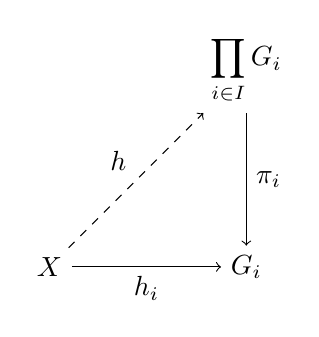
\begin{tikzpicture}[node distance=2.5cm, auto]
	\node (P) {$\displaystyle\prod_{i \in I} \bm{G_i}$};
	\node (Ci) [below of=P] {$\bm{G_i}$};
	\node (X) [left of=Ci] {$\bm{X}$};
	\draw[->] (X) to node [swap] {$h_i$} (Ci);
	\draw[->, dashed] (X) to node {$h$} (P);
	\draw[->] (P) to node {$\pi_i$} (Ci);
\end{tikzpicture}
\end{figure}
\end{proposition}
\begin{proof}
Defina a função
	\begin{align*}
	\func{h}{X}{\prod_{i \in I} G_i}{x}{(h_i(x))_{i \in I}}.
	\end{align*}
Da propriedade universal para o produto de conjuntos, $h$ é a única função tal que, para todo $i \in I$, $\pi_i \circ h = h_i$. Basta mostrar que $h$ é homomorfismo de grupos. Por simplicidade, apenas a operação $\times$ em $G$ será explicitada. Sejam $x_1,x_2 \in X$. Então, como $h_i$ são homomorfismos de grupo,
	\begin{equation*}
	h(x_1x_2) = (h_i(x_1x_2))_{i \in I} = (h_i(x_1)h_i(x_2))_{i \in I} = h(x_1)h(x_2).
	\end{equation*}
\end{proof}

\subsection{Grupo livre}

\begin{definition}
Seja $C$ um conjunto. O \emph{conjunto de inversos formais} de $C$ é o conjunto $C\inv := C \times \{-1\}$ e seus elementos são denotados $c\inv := (c,-1)$.

Uma \emph{palavra} em $C$ é uma sequência finita $(c_1,\ldots,c_n) \in C^n$. Denota-se $c_1 \cdots c_n$.
\end{definition}

Seja $p=c_1 \cdots c_n$ uma palavra em $C$. A \emph{palavra inversa} de $p$ é a palavra $p\inv := c_n\inv \cdots c_1\inv$.

\begin{definition}
Seja $C$ um conjunto e $p_1,p_2 $ palavras em $C \times \{1,-1\}$. A relação de equivalência entre as palavras $p_1$ e $p_2$ é definida por
	\begin{equation*}
	p_1 \sim p_2 \sse p_1p_2\inv \leadsto e.
	\end{equation*}	
\end{definition}

	\begin{equation*}
	C^* := \bigcup_{n \in \N} (C \times \{1,-1\})^n
	\end{equation*}
 Define-se $C^0 = \{\emptyset\}$.

	\begin{equation*}
	\ger{C} := C^*/\sim
	\end{equation*}
	
	A inclusão é definida.
	\begin{align*}
	\func{\iota}{C}{\ger{C}}{c}{[c]}.
	\end{align*}

\begin{proposition}[Propriedade Universal]
Seja $C$ um conjunto, $\bm X = (X,\star)$ um grupo e $f: C \to X$ uma função. Então existe um único homomorfismo de grupos $h: \bm{\ger{C}} \to \bm X$ tal que $h \circ \iota = f$ (o diagrama comuta).
\begin{figure}
\centering
\begin{tikzpicture}[node distance=2.5cm, auto]
	\node (C) {$C$};
	\node (G) [above of=C] {$\displaystyle\bm{\ger{C}}$};
	\node (X) [right of=C] {$\bm X$};
	\draw[->] (C) to node [swap] {$f$} (X);
	\draw[->, dashed] (G) to node {$h$} (X);
	\draw[->] (C) to node {$\iota$} (G);
\end{tikzpicture}
\end{figure}
\end{proposition}
\begin{proof}
Defina a função
	\begin{align*}
	\func{h}{\ger{C}}{X}{\left[c_1 \cdots c_n\right] }{f(c_1) \star \cdots \star f(c_n)},
	\end{align*}
de modo que $h([e])=e_X$. Então, para todo $c \in C$,
	\begin{equation*}
	h \circ \iota(c) = h (\iota(c)) = h([c])=f(c).
	\end{equation*}
Logo $h \circ \iota = f$. Para mostrar que é um homomorfismo de grupos, sejam $[c_1 \cdots c_n],$ $[d_1 \cdots d_m] \in \ger{C}$. Então
	\begin{align*}
	h([c_1 \cdots c_n][d_1 \cdots d_m]) &= h([c_1 \cdots c_nd_1 \cdots d_m]) \\
		&= f(c_1) \star \cdots \star f(c_n) \star f(d_1) \star \cdots  \star f(d_m) \\
		&= h([c_1 \cdots c_n]) \star h([d_1 \cdots d_m]).
	\end{align*}
Isso mostra a existência. Para mostrar a unicidade, seja $\overline h: \bm{\ger{C}} \to \bm X$ um homomorfismo de grupos tal que $\overline h \circ \iota = f$. Seja $[c_1 \cdots c_n] \in \ger{C}$. Como $[c_1 \cdots c_n] = [c_1] \cdots [c_n] = \iota(c_1) \cdots \iota(c_n)$, segue que
	\begin{align*}
	\overline h ([c_1 \cdots c_n]) &= \overline h(\iota(c_1) \cdots \iota(c_n)) \\
		&= \overline h(\iota(c_1)) \star \cdots \star \overline h(\iota(c_n)) \\
		&= f(c_1) \star \cdots \star f(c_n) \\
		&= h([c_1 \cdots c_n]),
	\end{align*}
o que implica que $\overline h = h$.
\end{proof}

\subsection{Coproduto de grupos}

\begin{definition}
Seja $(\bm{G_i})_{i \in I}$ uma família de grupos. O \emph{coproduto} da família $(\bm{G_i})_{i \in I}$ é o par
	\begin{equation*}
	\coprod_{i \in I} \bm{G_i} := \left(G,\times \right),
	\end{equation*}
em que $G := \ger{\coprod_{i \in I} G_i}$ é o grupo livre sobre o coproduto de conjuntos $\coprod_{i \in I} G_i$ e
	\begin{align*}
	\func{\times}{G \times G}{G}{([p_1],[p_2])}{[p_1p_2]}.
	\end{align*}
\end{definition}

\begin{proposition}[Propriedade Universal]
Sejam $(\bm{G_i})_{i \in I}$ uma família de grupos, $\bm X = (X,\star)$ um grupo e, para todo $i \in I$, $h_i: \bm{G_i} \to \bm X$ um homomorfismo de grupos. Então existe um único homomorfismo de grupos $h: \coprod_{i \in I} \bm{G_i} \to \bm X$ tal que, para todo $i \in I$, $h \circ \iota_i = h_i$ (o diagrama comuta).
\begin{figure}
\centering
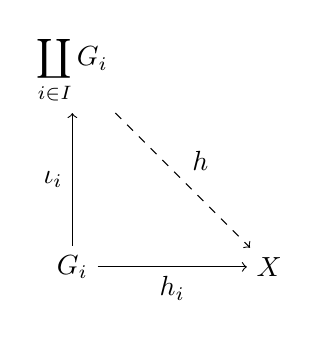
\begin{tikzpicture}[node distance=2.5cm, auto]
	\node (Ci) {$\bm{G_i}$};
	\node (S) [above of=Ci] {$\displaystyle\coprod_{i \in I} \bm{G_i}$};
	\node (X) [right of=Ci] {$\bm X$};
	\draw[->] (Ci) to node [swap] {$h_i$} (X);
	\draw[->, dashed] (S) to node {$h$} (X);
	\draw[->] (Ci) to node {$\iota_i$} (S);
\end{tikzpicture}
\end{figure}
\end{proposition}
\begin{proof}
Defina a função
	\begin{align*}
	\func{h}{\ger{\coprod_{i \in I} G_i}}{X}{\left[(g_1,i_1) \cdots (g_n,i_n)\right]}{h_{i_1}(g_1) \star \cdots \star h_{i_n}(g_n)}.
	\end{align*}

Por simplicidade, seja $G := \ger{\coprod_{i \in I} G_i}$. Para mostrar que $h$ é homomorfismo, sejam $[(g_1,i_1) \cdots (g_n,i_n)]$ e $[(g'_1,i'_1) \cdots (g'_m,i'_m)] \in G$. Então
	\begin{align*}
	&h([(g_1,i_1) \cdots (g_n,i_n)][(g'_1,i'_1) \cdots (g'_m,i'_m)]) \\
		&= h([(g_1,i_1) \cdots (g_n,i_n)(g'_1,i'_1) \cdots (g'_m,i'_m)]) \\
		&= h_{i_1}(g_1) \star \cdots \star h_{i_n}(g_n) \star h_{i'_1}(g'_1) \star \cdots \star h_{i'_n}(g'_n) \\
		&= h([(g_1,i_1) \cdots (g_n,i_n)]) \star h([(g'_1,i'_1) \cdots (g'_m,i'_m)]).
	\end{align*}
\end{proof}








































\cleardoublepage
\section{Construções específicas}

\subsection{Translações e conjugações}

\begin{definition}
Sejam $\bm G$ um grupo e $g \in G$. A \emph{conjugação} por $g$ é a função
	\begin{align*}
	\func{C_g}{G}{G}{h}{ghg\inv},
	\end{align*}
a \emph{translação à direita} por $g$ é a função
	\begin{align*}
	\func{D_g}{G}{G}{h}{hg}
	\end{align*}
e a \emph{translação à esquerda} por $g$ é a função
	\begin{align*}
	\func{E_g}{G}{G}{h}{gh}.
	\end{align*}
\end{definition}

\begin{proposition}
Sejam $\bm G$ um grupo e $g \in G$. As funções $C$, $D$ e $E$ são bijeções.
\end{proposition}
\begin{proof}
Basta mostrarmos para $D_g$ e $E_g$, pois $C_g = E_{g} \circ D_{g\inv}$. Primeiro, mostremos que as translações são homomorfismos. Para todos $g,g',h \in G$,
	\begin{equation*}
		E_{g} \circ E_{g'}(h) = gg'h = E_{gg'}(h)
	\end{equation*}
e
	\begin{equation*}
		D_{g} \circ D_{g'}(h) = hg'g = D_{g'g}(h),
	\end{equation*}
o que mostra que $E_{gg'} = E_g \circ E_{g'}$

Isso mostra que as translações à esquerda e à direita têm inversa $E_{g\inv}$ e $D_{g\inv}$, respectivamente, pois
	\begin{equation*}
		E_{g} \circ E_{g\inv} = E_{gg\inv} = \Id = E_{g\inv g} = E_{g\inv} \circ E_{g}
	\end{equation*}
e
	\begin{equation*}
		D_{g} \circ D_{g\inv} = D_{gg\inv} = \Id = D_{g\inv g} = D_{g\inv} \circ D_{g}.
	\end{equation*}
\end{proof}

\begin{proposition}
Sejam $\bm G$ um grupo e $g \in G$. A conjugação $C_g$ é isomorfismo de grupo.
\end{proposition}
\begin{proof}
Como $C_g$ é bijeção, basta mostrar que é homomorfismo de grupo. Para todos $h,h' \in G$,
	\begin{equation*}
		C_g(hh') = ghh'g\inv = ghg\inv gh'g\inv = C_g(h)C_g(h').
	\end{equation*}
\end{proof}

A \emph{conjugação} em $\bm G$ é a função
	\begin{align*}
		\func{C}{G}{\Iso{\Homo}(G)}{g}{C_g}
	\end{align*}

%A \emph{translação à direita} em $\bm G$ é a função
%	\begin{align*}
%		\func{D}{G}{\Iso{\Func}(G)}{g}{D_g}
%	\end{align*}
%
%A \emph{translação à esquerda} em $\bm G$ é a função
%	\begin{align*}
%		\func{E}{G}{\Iso{\Func}(G)}{g}{E_g}
%	\end{align*}

\subsection{Centro, automorfismos internos e externos}

\begin{definition}
Seja $\bm G$ um grupo. O \emph{centro} de $\bm G$ é o conjunto
	\begin{equation*}
		\Zen(G) := \set{g \in G}{\forall_{h \in G}\ C_g(h)=h}
	\end{equation*}
\end{definition}


Notemos que, como $C$ é homomorfismo de grupos e 
	\begin{align*}
		\Zen(G) &= \set{g \in G}{\forall_{h \in G}\ C_g(h) = h} \\
				&= \set{g \in G}{C_g = \Id} \\
				&= \nuc{C},
	\end{align*}
o centro de $\bm G$ é um subgrupo normal de $\bm G$.

\begin{definition}
Seja $\bm G$ um grupo. Um \emph{automorfismo interno} de $\bm G$ é um automorfismo da forma $C_g$ para algum $g \in G$.
\end{definition}

Pode-se mostrar que um automorfismo $\fun{h}{G}{G}$ é interno (ou seja, é conjugação por algum elemento de $G$) se, e somente se, para todo supergrupo $\bm H \geq \bm G$, esse automorfismo pode ser estendido para $\bm H$. A ida é evidente mas a volta é um pouco mais complicada\cite{art:Schupp-CharacterizationInnerAutomorphisms}.

	\begin{equation*}
	1 \to \Zen(G) \to G \to \Aut(G) \to Out(G) \to 1
	\end{equation*}


\subsection{Centralizador e normalizador}






\subsection{Produto semidireto}

\begin{definition}
Sejam $\bm G$ e $\bm H$ grupos e $A\colon \bm G \age \bm H$ uma ação do grupo $\bm G$ sobre o grupo $\bm H$. O \emph{produto semidireto} (à esquerda) de $\bm H$ por $\bm G$ com respeito a $A$ é o grupo
	\begin{equation*}
		\bm G \ltimes_A \bm H := (G \times H,\times_{G \ltimes_A H},\div_{G \ltimes_A H},\id_{G \ltimes_A H})
	\end{equation*}
em que
	\begin{align*}
		\func{\times_{G \ltimes_A H}}{(G \times H) \times (G \times H)}{G \times H}{((g,h),(g',h'))}{(gg',hA_g(h'))},
	\end{align*}
	\begin{align*}
		\func{\div_{G \ltimes_A H}}{G \times H}{G \times H}{(g,h)}{(g\inv,A_{g\inv}(h\inv))}
	\end{align*}
e
	\begin{equation*}
		\id_{G \ltimes_A H} := (\id_G,\id_H).
	\end{equation*}
Por simplicidade, denotamos $G \ltimes H$ quando a ação está subentendida no contexto.

%O \emph{produto semidireto} (à direita) de $\bm H$ por $\bm G$ com respeito a $A$ é o grupo
%		\begin{equation*}
%			\bm H \rtimes_A \bm G := (H \times G,\times_A,\div_A,\id_A)
%		\end{equation*}
%	em que
%		\begin{align*}
%			\func{\times_A}{(H \times G) \times (H \times G)}{H \times G}{((h,g),(h',g'))}{(A_g(h'),g'g)}
%		\end{align*}
\end{definition}

O produto semidireto à direita é definido analogamente e denotado $\bm H \rtimes_A \bm G$, com
	\begin{align*}
		\func{\times_{H \rtimes G}}{(H \times G) \times (H \times G)}{H \times G}{((h,g),(h',g'))}{(A_g(h')h,gg')}
	\end{align*}
e as mesmas inversa e identidade do caso à esquerda. Vale ressaltar que com uma ação do grupo $\bm G$ sobre o grupo $\bm H$ queremos dizer um homomorfismo de grupos
	\begin{equation*}
		A\colon \bm G \to \Iso{\Homo}(\bm H),
	\end{equation*}
em que $\Iso{\Homo}(\bm H)$ é o grupo dos automorfismos de grupo de $\bm H$.

% Qual a relação da ação ser à esquerda/direita com o produto semidireto ser à esquerda/direita?

\begin{exercise}
Sejam $\bm G$ e $\bm H$ grupos e $A\colon \bm G \age \bm H$ uma ação do grupo $\bm G$ sobre o grupo $\bm H$.
	\begin{enumerate}
		\item O produto semidireto $\bm G \ltimes_A \bm H$ é um grupo.
		
		\item $\bm G \simeq \bm G \ltimes \bm{\{\id_H\}} \leq \bm G \ltimes \bm H$, e $\bm G \ltimes \bm{\{\id_H\}} \ide \bm G \ltimes \bm H$ se, e somente se, $\bm G \ltimes \bm H = \bm G \times \bm H$ (ou $A=\Id_H$);
		
		\item $\bm H \simeq \bm{\{\id_G\}} \ltimes \bm H \ide \bm G \ltimes \bm H$;
	\end{enumerate}
\end{exercise}

\begin{example}
	\begin{enumerate}
		\item O produto direto de grupos $\bm G$ e $\bm H$ é um produto semidireto cuja ação é a função constante
	\begin{align*}
		\func{\Id_H}{G}{\Iso{\Homo}(H)}{g}{
			\begin{aligned}[t]
				\func{\Id_H}{H}{H}{h}{h}
			\end{aligned}
		}
	\end{align*}

	\item Seja $n \in \N$. $\OO(n) \simeq \S^0 \ltimes \SO(n)$ com ação dada por
		\begin{align*}
			\func{A}{\S^0}{\Aut(\SO(n))}{i}{
				\begin{aligned}[t]
					\func{C_{\Id_{n-1} \oplus i}}{\SO(n)}{\SO(n)}{N}{(\Id_{n-1} \oplus i) \circ N \circ (\Id_{n-1} \oplus i)\inv}.
				\end{aligned}
			}
		\end{align*}
	A transformação linear $\Id_{n-1} \oplus i \in \OO(n)$ é uma reflexão de $\R^n$ que pode ser representada pela matrix
		\begin{equation*}
			\begin{pmatrix}
				\Id_{n-1}	&	0 \\
				0			&	i
			\end{pmatrix}.
		\end{equation*}
	\end{enumerate}
\end{example}













\subsection{Grupo simples e subgrupo normal maximal}

\begin{definition}
Um \emph{grupo simples} é um grupo não-trivial $\bm G$ cujos únicos subgrupos normais são $\bm{\{1\}}$ e $\bm G$.
\end{definition}

\begin{definition}
Seja $\bm G$ um grupo. Um subgrupo normal \emph{maximal} de $\bm G$ é um subgrupo normal próprio $\bm M \idepro \bm G$ que satisfaz
	\begin{enumerate}
	\item (Maximalidade) Para todo $\bm N \ide \bm G$,
		\begin{equation*}
		M \subseteq N \Rightarrow N = M \text{\ \ ou\ \ } N = G.
		\end{equation*}
	\end{enumerate}
\end{definition}

\begin{proposition}
Sejam $\bm G$ um grupo e $\bm M \ide \bm G$ um subgrupo normal. Então $\bm M$ é maximal se, e somente se, $\bm{G/M}$ é simples.
\end{proposition}
\begin{proof} Consideremos a projeção canônica
	\begin{align*}
	\func{\pi}{G}{\quo{G}{M}}{g}{gM}.
	\end{align*}
	\begin{enumerate}
		\item [($\Rightarrow$)] Suponhamos que $\bm M$ é maximal. Então $\bm M$ é um subgrupo próprio, o implica que $\bm{G/M}$ é não-trivial. Seja $\bm N \ide \bm{G/M}$. Sabemos que $\bm{\pi^{-1}(N)} \ide \bm G$ (\ref{alge:prop.gru.hominv}). Como $[e] \in N$, então $\pi^{-1}(1) \subseteq \pi^{-1}(N)$. Notando que $\pi^{-1}([1])=\nuc(\pi) = M$, segue que $M \subseteq \pi^{-1}(N)$. Como $\bm M$ é maximal, segue que $\pi^{-1}(N) = N$ ou $\pi^{-1}(N) = G$. Notemos que $N=\pi(\pi^{-1}(N))$, pois $\pi$ é sobrejetiva. No primeiro caso, $N = \pi(\pi^{-1}(N)) = \pi(M) = \{[1]\}$. No segundo caso, $N = \pi(\pi^{-1}(N)) = \pi(G) = G/M$. Portanto $\bm{G/M}$ é simples.
		
		\item [($\Leftarrow$)] Suponhamos que $\bm{G/M}$ é simples. Seja $\bm N \ide \bm G$ tal que $M \subseteq N$. Como $\pi$ é homomorfismo de grupos sobrejetivo, segue que $\pi(N) \ide \bm{G/M}$ (\ref{alge:prop.gru.hom}). Como $\bm{G/M}$ é simples, então $\pi(N) = \{[e]\}$ ou $\pi(N) = G/M$. No primeiro caso, $N = \nuc(\pi) = M$. No segundo caso, $N = \pi^{-1}(\pi(N)) = \pi^{-1}(N) = G$. Logo $\bm M$ é maximal.
	\end{enumerate}
\end{proof}

\begin{conjecture}
Sejam $\bm G$ um grupo e $\bm N \idepro \bm G$ um subgrupo normal próprio. Então $\bm G$ tem subgrupo normal maximal.
\end{conjecture}
\begin{proof}
Usaremos o lema de Zorn. Seja $P \subseteq \p(G)$ o conjunto de todos os subconjuntos $S \subset G$ tais que $\bm S \idepro \bm G$. Então $(P,\subseteq)$ é um conjunto parcialmente ordenado com a contenção de conjuntos usual. Agora, seja $(C)_{i \in I}$ uma cadeia de $(P,\subseteq)$. Consideremos o conjunto $C := \bigcup_{i \in I} C_i$. Como 

Notemos que $P$ não é vazio, pois $N \in P$. Seja



Então $P$ tem elemento maximal.
\end{proof}






\subsection{Sequência subnormal}

\begin{definition}
Seja $\bm G$ um grupo. Uma \emph{sequência subnormal} de $\bm G$ é uma sequência finita $(\bm{N_i})_{i \in [n]}$ de subgrupos de $\bm G$ que satisfaz
	\begin{equation*}
	\bm{\{1\}} = \bm{N_0} \ide \cdots \ide \bm{N_{n-1}} = \bm G.
	\end{equation*}
O grupo $\bm{N_{i+1}/N_i}$ é o $i$-ésimo \emph{grupo fator} da sequência.
Uma \emph{sequência normal} é uma sequência subnormal em que, para todo $i \in [n]$, $\bm{N_i} \ide \bm G$.

Uma sequência subnormal \emph{estrita} de $\bm G$ é uma sequência subnormal $(\bm{N_i})_{i \in [n]}$ de $\bm G$ que satisfaz
	\begin{equation*}
	\bm{\{1\}} = \bm{N_0} \idepro \cdots \idepro \bm{N_{n-1}} = \bm G.
	\end{equation*}
	
O \emph{comprimento} de uma sequência subnormal estrita é o número $n$.
\end{definition}



\subsection{Conjunto gerador}

\begin{definition}
Seja $\bm G$ um grupo e $S \subseteq G$ um conjunto. O grupo \emph{gerado} por $S$ é o grupo $\bm{\langle S \rangle} \leq \bm G$ em que
	\begin{equation*}
	\langle S \rangle := \set{s_1 \cdots s_n}{n \in \N,\ s_i \in S \text{\ \ ou\ \ } s_i\inv \in S}.
	\end{equation*}
	\begin{equation*}
	\langle S \rangle := \set{\bigopb_{i \in [n]} s_i}{n \in \N,\ s_i \in S \text{\ \ ou\ \ } s_i\inv \in S}.
	\end{equation*}
\noindent
Um \emph{conjunto gerador} de $\bm G$ é um conjunto $S \subseteq G$ tal que $\langle S \rangle = G$.
\end{definition}









\section{Ação de grupos}

\subsection{Grupo simétrico}

Para falar de ação de grupo, primeiro demonstraremos que o conjunto de bijeções de um conjunto para si mesmo é um grupo com as operações de composição, inversa de função e função identidade.

\begin{definition}
Seja $C$ um conjunto. O \emph{grupo simétrico} (ou \emph{grupo de bijeções}) de $C$ é a lista
	\begin{equation*}
	\Iso{\bm{\Func}}(C) = (\Iso{\Func}(C),\circ,\inv,\Id),
	\end{equation*}
em que $\Iso{\Func}(C)$ é o conjunto de bijeções de $C$ para $C$, $\circ$ é a composição de funções, $\inv$ é a inversa de funções e $\Id$ é a função identidade.
%Seja $\alpha$ um número cardinal. Para $C = \alpha$, usa-se a notação $\sime_{\alpha} := \Iso{\Func}(\alpha)$.
\end{definition}

\begin{proposition}
Seja $C$ um conjunto. O grupo simétrico $\Iso{\bm{\Func}}(C)$ é um grupo.
\end{proposition}
\begin{proof}
Se $C=\emptyset$, então $\Iso{\Func}(C)=\{\emptyset\}$. Assim, como $\emptyset \circ \emptyset = \emptyset$, segue que $\circ$ é operação binária em $\{\emptyset\}$. Ainda, segue que $\circ$ é associativa, pois $(\emptyset \circ \emptyset) \circ \emptyset = \emptyset \circ (\emptyset \circ \emptyset)$; tem elemento neutro $\emptyset$, pois $\emptyset \circ \emptyset = \emptyset$, e que todo elemento tem inverso, pois $\emptyset\inv = \emptyset$.

Suponhamos, então, que $C \neq \emptyset$ e sejam $p_1,p_2 \in \Iso{\Func}(C)$. Como $p_1$ e $p_2$ são bijeções, a função $p_2 \circ p_1: C \to C$ é uma bijeção entre $C$ e $C$ (\ref{prop:comp.func.inj} e \ref{prop:comp.func.sobr}) e, portanto, $p_2 \circ p_1 \in \Iso{\Func}(C)$. Isso mostra que $\circ$ é uma operação binária em $\Iso{\Func}(C)$.
	\begin{enumerate}
		\item A composição de funções é associativa, pois, para todos $p_1,p_2,p_3 \in \Iso{\Func}(C)$, $p_3 \circ (p_2 \circ p_1) = (p_3 \circ p_2) \circ p_1$ (\ref{prop:comp.func.asso}).

		\item Ainda, notemos que $\Id_C$ é o elemento neutro de $\Iso{\bm{\Func}}(C)$, pois, para todo $p \in \Iso{\Func}(C)$, vale $p \circ \Id_C = \Id_C \circ p = p$ (\ref{prop:id.comp.func}).

		\item Por fim, como $p$ é uma bijeção, existe função inversa $p\inv: C \to C$ que é bijeção entre $C$ e $C$ (\ref{prop:func.inv.esq} e \ref{prop:func.inv.dir}); logo existe $p\inv \in \Iso{\Func}(C)$ tal que $p \circ p\inv = p\inv \circ p = \Id_C$.
	\end{enumerate}
Portanto concluímos que $\Iso{\bm{\Func}}(C)$ é um grupo.
\end{proof}

\begin{proposition}
	Sejam $A$ e $B$ conjuntos tais que $\card{A} = \card{B}$. Então
	\begin{equation*}
	\Iso{\bm{\Func}}(A) \simeq \Iso{\bm{\Func}}(B).
	\end{equation*}
\end{proposition}
\begin{proof}
	Seja $\phi: A \to B$ uma bijeção e considere a função
	\begin{align*}
	\func{h}{\Iso{\Func}(A)}{\Iso{\Func}(B)}{p}{\phi \circ p \circ \phi\inv}.
	\end{align*}
Primeiro notemos que $h$ é homomorfismo de grupos. Sejam $p_1,p_2 \in \Iso{\Func}(A)$. Então
	\begin{align*}
	h(p_2 \circ p_1)(c) &= \phi \circ (p_2 \circ p_1) \circ \phi^{-1} \\
			&= \phi \circ (p_2 \circ \phi\inv \circ \phi \circ p_1) \circ \phi^{-1} \\
			&= (\phi \circ p_2 \circ \phi\inv) \circ (\phi \circ p_1 \circ \phi\inv) \\
			&= h(p_2) \circ h(p_1).
	\end{align*}
Portanto $h$ é um homomorfismo de grupos entre $\Iso{\bm{\Func}}(A)$ e $\Iso{\bm{\Func}}(B)$.

Agora notemos que $h$ é uma bijeção. A inversa de $h$ é a função
	\begin{align*}
	\func{h\inv}{\Iso{\Func}(B)}{\Iso{\Func}(A)}{p}{\phi\inv \circ p \circ \phi},
	\end{align*}
pois, para todo $p \in \Iso{\Func}(B)$,
	\begin{align*}
	(h \circ h\inv) (p) &= h (h\inv(p)) \\
			&= \phi \circ h\inv(p) \circ \phi\inv \\
			&= \phi \circ (\phi\inv \circ p \circ \phi) \circ \phi\inv \\
			&= p \\
			&= 1_{\Iso{\Func}(B)}(p),
	\end{align*}
o que mostra que $h \circ h\inv = 1_{\Iso{\Func}(B)}$, e, para todo $p \in \Iso{\Func}(A)$,
	\begin{align*}
	(h\inv \circ h) (p) &= h\inv (h(p)) \\
			&= \phi\inv \circ h(p) \circ \phi \\
			&= \phi\inv \circ (\phi \circ p \circ \phi\inv) \circ \phi \\
			&= p \\
			&= 1_{\Iso{\Func}(A)}(p),
	\end{align*}
o que mostra que $h\inv \circ h = 1_{\Iso{\Func}(A)}$. Assim, está provado que $h$ é isomorfismo entre $\Iso{\bm{\Func}}(A)$ e $\Iso{\bm{\Func}}(B)$.
\end{proof}

	Essa proposição mostra que podemos estudar somente os grupos simétricos dos números cardinais, pois isso será equivalente a estudar qualquer grupo simétrico. Em particular, para todo conjunto finito, podemos estudar seu grupo simétrico considerando somente o grupo simétrico $\bm\sime_n$, em que $n$ é o número de elementos do conjunto. A partir de agora, as proposições serão considerando esses grupos $\bm\sime_n$.

\begin{theorem}
	Seja $\bm G$ um grupo. Então
	\begin{equation*}
	\bm G \lesssim \Iso{\bm{\Func}}(G).
	\end{equation*}
\end{theorem}
\begin{proof}
	Consideremos a função
	\begin{align*}
	\func{h}{G}{\Iso{\Func}(G)}{g}{
		\begin{aligned}[t]
		\func{h(g)}{G}{G}{x}{g \times x}
		\end{aligned}
	}
	\end{align*}
Primeiro, devemos mostrar que $h(g) \in \Iso{\Func}(G)$, para que $h$ esteja bem definida. Para isso, notemos que $h(g)$ está bem definida, já que, para todo $x \in G$, $g \times x \in G$. Ainda, $h(g)$ é uma bijeção, pois $h(g)\inv = h(g\inv)$, já que, para todo $x \in G$,
	\begin{equation*}
	(h(g) \circ h(g)\inv)(x) = h(g)((h(g)\inv)(x)) = h(g)(g\inv \times x) = g \times g\inv \times x = x = 1_G,
	\end{equation*}
o que mostra que $h(g) \circ h(g)\inv = 1_G$, e
	\begin{equation*}
	(h(g)\inv \circ h(g))(x) = h(g)\inv((h(g)(x)) = h(g)\inv(g \times x) = g\inv \times g \times x = x = 1_G,
	\end{equation*}
o que mostra que $h(g)\inv \circ h(g) = 1_G$. Isso mostra que $h(g)$ é uma bijeção e, portanto, $h(g) \in \Iso{\Func}(G)$.

	Agora, notemos que $h$ é um homomorfismo de grupos, pois, para todos $g_1,g_2 \in G$, segue que, para todo $x \in G$,
	\begin{align*}
	h(g_1 \times g_2)(x) &= (g_1 \times g_2) \times x \\
	&= g_1 \times (g_2 \times x) \\
	&= h(g_1)(g_2 \times x) \\
	&= h(g_1)(h(g_2)(x)) \\
	&= (h(g_1) \circ h(g_2))(x),
	\end{align*}
o que mostra que $h(g_1 \times g_2) = h(g_1) \circ h(g_2)$. Por fim, notemos que $h$ é injetiva, já que, se $g \in G$ é tal que $h(g)=id_G$, então, para todo $x \in G$,
	\begin{equation*}
	g \times x = h(g)(x) = 1_G(x) = x,
	\end{equation*}
o que mostra que $g=e_G$ e, portanto, que $\nuc(h)=\{e_G\}$.
\end{proof}

	Esse teorema é um teorema muito importante, pois ele mostra que, de certa forma, todo grupo é um subconjunto de permutações. Por causa disso que grupos são pensados como os objetos algébricos que modelam a simetria.

\subsection{Ações}

A noção de uma ação de grupo, de certa forma, generaliza uma estratégia usada na demonstração do teorema de que todo grupo é isomorfo a um subgrupo de seu grupo simétrico.

\begin{definition}
Sejam $\bm G$ um grupo e $X$ um conjunto. Uma \emph{ação} de $\bm G$ em $X$ é um homomorfismo de grupos
	\begin{align*}
	\func{A}{G}{\Iso{\Func}(X)}{g}{
		\begin{aligned}[t]
		\func{g\pt}{X}{X}{x}{g\pt x}.
		\end{aligned}
	}
	\end{align*}
Denota-se $\acao{A}{\bm G}{X}$. Diz-se que o grupo $\bm G$ \emph{age} no conjunto $X$, e denota-se $\bm G \age X$, se, e somente se, existe ação de $\bm G$ em $X$.
%O grupo $\bm G$ é o \emph{grupo de funções} e o conjunto $X$ é um \emph{$\bm G$-conjunto}.
\end{definition}

A definição acima é uma definição muito simplificada pois ela depende de conceitos um pouco mais complexos, como de homomorfismo de grupos e de grupo de bijeções. A proposição abaixo mostra como essa definição é equivalente a uma definição mais explícita de ação de grupo que também é comumente usada.

\begin{proposition}
Sejam $X$ um conjunto e $\bm G$ um grupo. Então $\bm G \age X$ se, e somente se, existe uma função
	\begin{align*}
	\func{\pt}{G \times X}{X}{(g,x)}{g\pt x}
	\end{align*}
que satisfaz
\begin{enumerate}
\item (Identidade) Para todo $x \in X$,
	\begin{equation*}
	e \pt x = x;
	\end{equation*}
\item (Compatibilidade) Para todos $g_0,g_1 \in G$ e $x \in X$,
	\begin{equation*}
	(g_1g_0) \pt x = g_1 \pt (g_0 \pt x).
	\end{equation*}
\end{enumerate}
\end{proposition}
\begin{proof}
Se existe ação $\acao{A}{\bm G}{X}$, basta definir $g \pt x := A(g)(x)$ e segue que $e\pt = 1$ e $(g_1g_0) \pt = (g_1 \pt) \circ (g_0 \pt)$. Reciprocamente, definimos a ação $A$ a partir de $\pt$ da mesma forma e, se $g_0,g_1 \in G$ e $x \in X$, segue que
	\begin{equation*}
	A(g_1g_0)(x) =(g_1g_0) \pt x = g_1 \pt (g_0 \pt x) = A(g_1)(A(g_0)(x)) = A(g_1) \circ A(g_0)(x),
	\end{equation*}
logo $A(g_1g_0)=A(g_1) \circ A(g_0)$.
\end{proof}

Essa proposição é geralmente considerada a definição de uma ação \emph{à esquerda} de $\bm G$ em $X$ por causa da posição em que a composição ocorre. Analogamente, uma ação à direita pode ser definida, mas toda ação à direita pode ser traduzida em uma ação à esquerda, de modo que é suficiente estudar somente ações à esquerda. É comum, ainda, estudar ações em conjuntos $X$ com alguma estrutura adicional, geralmente uma topologia. Nesse caso, exige-se que a ação seja uma função contínua, mas também é necessário que $G$ tenha uma estrutura topológica, portanto isso não será definido com cuidado agora.

\subsection{Órbitas e estabilizadores}

\begin{definition}
Sejam $X$ um conjunto, $\bm G$ um grupo, $\bm G \age X$ e $x \in X$. A \emph{órbita} de $x$ sob $\bm G$ é o conjunto
	\begin{equation*}
	G \pt x := \set{g\pt x}{g \in G}.
	\end{equation*}
\end{definition}

\begin{definition}
Sejam $X$ um conjunto, $\bm G$ um grupo, $A: \bm G \age X$ e $x \in X$. O \emph{estabilizador} de $x$ é
	\begin{equation*}
	G_x = \set{g \in G}{g\pt x = x} = A\inv(\{1\}) = \nuc(A).
	\end{equation*}
\end{definition}

O estabilizador de $x$ é um grupo e por isso é chamado de \emph{subgrupo estabilizador} de $\bm G$ com respeito a $x$, e também é conhecido como \emph{grupo de isotropia} de $x$.







\subsection{Permutações finitas}


\begin{exercise}
Seja $n \in \N$. Então $|\sime_n|=n!$.
\end{exercise}


\begin{definition}
Seja $n \in \N$. Uma \emph{permutação} de $n$ objetos é um elemento $p \in \sime_n$, denotado por
	\begin{equation*}
	p = \begin{pmatrix}
				1 & 2 & \cdots & n-1 & n \\
				p(1) & p(2) & \cdots &  p(n-1)  & p(n)
			\end{pmatrix}.
	\end{equation*}
\end{definition}

\begin{notation}
Seja $n \in \N$. A composição de duas permutações $p_1,p_2 \in \sime_n$, quando representadas na notação acima, é denotada
	\begin{equation*}
	p_2 \circ p_1 = \bigl(\begin{smallmatrix}
				1 & 2 & \cdots & n-1 & n \\
				p_2(1) & p_2(2) & \cdots &  p_2(n-1)  & p_2(n)
			\end{smallmatrix}\bigr)
			\bigl(\begin{smallmatrix}
				1 & 2 & \cdots & n-1 & n \\
				p_1(1) & p_1(2) & \cdots &  p_1(n-1)  & p_1(n)
			\end{smallmatrix}\bigr).
	\end{equation*}
\end{notation}

\begin{definition}
	Sejam $n \in \N$ e $p \in \sime_n$. A \emph{matriz de permutação} de $p$ é a matriz $[p] \in \M_n (\Z)$ cujas entradas são dadas por
	\begin{equation*}
		[p]_{i,j} = \delta_{i,p(j)} = \begin{cases}
												1 & i=p(j) \\
												0 & i \neq p(j).
												\end{cases}
	\end{equation*}
	O \emph{conjunto das matrizes de permutação} de $\sime_n$ é o conjunto
	\begin{equation*}
		[\sime_n] := \set{[p]}{p \in \sime_n}.
	\end{equation*}
\end{definition}

\begin{proposition}
	Seja $n \in \N$. Então o par $\bm{[\sime_n]}=([\sime_n],\cdot)$, em que $\cdot$ é o produto de matrizes, é um grupo, e
	\begin{equation*}
	\bm{\sime_n} \simeq \bm{[\sime_n]}.
	\end{equation*}
\end{proposition}
\begin{proof}
	Primeiro, notemos que, para todos $p,q \in \sime_n$,
	\begin{equation*}
	[p][q]_{i,j} = \sum_{k=0}^{n-1} [p]_{i,k}[q]_{k,j} = \sum_{k=0}^{n-1} \delta_{i,p(k)}\delta_{k,p(j)}.
	\end{equation*}
	Mas o produto $\delta_{i,p(k)}\delta_{k,p(j)}$ é igual a 1 se, e somente se, $i=p(k)$ e $k=q(j)$. Como $p$ é bijeção, a segunda condição é equivalente a $p(k)=pq(j)$, e isso mostra que as duas condições são equivalentes a $i=p(k)=pq(j)$. Como $p$ é bijeção, para cada $i \in [n]$, $k=p\inv(i)$ é o único $k \in [n]$ tal que a condição é satisfeita, e segue que
	\begin{equation*}
	[p][q]_{i,j} = \sum_{k=1}^n \delta_{i,p(k)}\delta_{k,p(j)} = \sum_{k=1}^n \delta_{i,pq(j)} = [pq]_{i,j}.
	\end{equation*}
e, como $pq \in \sime_n$, então $[p][q]=[pq] \in [\sime_n]$. Isso mostra que o produto de matrizes é uma operação binária em $[\sime_n]$. Agora, disso segue que $[p][p\inv]=[pp\inv]=[id]$

%MOSTRAR QUE O INVERSO DE P ESTA NO GRUPO




Disso, segue que $\bm{[\sime_n]}$ é um grupo, pois é subgrupo de $\M_n(\Z)$. Por fim, consideremos a função
	\begin{align*}
	\func{h}{\sime_n}{[\sime_n]}{p}{[p]}.
	\end{align*}
Note que que $h$ é homomorfismo, pois, para todos $p,q \in \sime_n$,
	\begin{equation*}
	h(pq) = [pq]= [p][q] = h(p)h(q).
	\end{equation*}
Ainda, $h$
\end{proof}

\begin{definition}
	Sejam $n \in \N$, $p \in \sime_n$ e $m \in [n]$. A \emph{órbita de $m$ sob $p$} é o conjunto
	\begin{equation*}
	\orb_p(m) := \set{p^k(m)}{k \in \Z}.
	\end{equation*}
O \emph{período} da órbita $\orb_p(m)$ é o número $\card{\orb_p(m)}$. Uma \emph{órbita trivial} é uma órbita de período $1$. Uma órbita de $p$ é a órbita de um elemento $m \in [n]$ sob $p$.

	O \emph{conjunto de órbitas} de $p$ é o conjunto
	\begin{equation*}
	\orb_p := \set{\orb_p(m)}{m \in [n]}.
	\end{equation*}
\end{definition}

\begin{proposition}
	Sejam $n \in \N$ e $p \in \sime_n$. O conjunto $\orb_p$ é uma partição de $[n]$.
\end{proposition}
\begin{proof}
	Primeiro, notemos que $m \in \orb_p(m)$ e, portanto, $\emptyset \nsubseteq \orb_p$. Ainda, $\bigcup_{m \in [n]} \orb_p(m) = [n]$, já que, para todo $m \in [n]$, $m \in \orb_p(m)$, o que mostra que $[n] \subseteq \bigcup_{m \in [n]}$ e, para todo $l \in \bigcup_{m \in [n]} \orb_p(m)$, existe $m \in [n]$ tal que $l \in \orb_p(m)$ e, portanto, existe $k \in \N$ tal que $l=p^k(m) \in [n]$, o que mostra que $\bigcup_{m \in [n]} \subseteq [n]$. Por fim, sejam $o_1,o_2 \in \orb_p$. Então existem $m_1,m_2 \in [n]$ tais que $o_1=\orb_p(m_1)$ e $o_2=\orb_p(m_2)$. Se existe $l \in \orb_p(m_1) \cap \orb_p(m_2)$, então existem $k_1,k_2 \in \Z$ tais que $l=p^{k_1}(m_1)=p^{k_2}(m_2)$. Assim, segue que $m_1=p^{k_2-k_1}(m_2)$ e, portanto, $m_1 \in \orb_p(m_2)$. Mas isso implica que $\orb_p(m_1) \subseteq \orb_p(m_2)$; a inclusão contrária é análoga e concluímos que $\orb_p(m_1) = \orb_p(m_2)$. Logo $\orb_p$ é uma partição de $[n]$.
\end{proof}

\subsubsection{Ciclos e transposições}

\begin{definition}
	Sejam $n,k \in \N$. Um \emph{ciclo} de $\sime_n$ é um elemento $c \in \sime_n$ para o qual existe $m \in [n]$ tal que, para todo $m' \in [n]$, $c(m')=m'$ ou existe $d \in [n]$ tal que $m'=c^d(m)$. O \emph{comprimento} de um ciclo é a ordem desse ciclo. Um ciclo $c$ cujo comprimento é $k$ é denotado
	\begin{equation*}
	c = \bigl(m \ c(m) \ c^2(m) \ \cdots \  c^{k-2}(m) \ c^{k-1}(m)\bigr).
	\end{equation*}
\end{definition}


\begin{proposition}
	Sejam $n \in \N$.
	\begin{enumerate}
	\item Se $c_1,c_2 \in \sime_n$ são ciclos disjuntos, então $c_2 \circ c_1 = c_1 \circ c_2$.
	\end{enumerate}
\end{proposition}

\begin{proposition}[Fatoração de Permutação]
	Seja $n \in \N$ e $p \in \sime_n$. Então existem únicos ciclos $c_1,\ldots,c_k \in \sime_n$ disjuntos dois a dois tais que $p=c_1 \circ \cdots \circ c_k$.
\end{proposition}
\begin{proof}
	Seja $k := \card{\orb_p}$. O conjunto $\orb_p$ particiona $[n]$. Sejam $(o_k)_{i \in [k]}$ uma indexação de $\orb_p$ e $m_1,\cdot,m_k \in [n]$ tais que $o_i=\orb_p(m_i)$ para todo $i \in [k]$, e seja $k_i := \card{\orb_p(m_i)}$. Definamos $c_i :=  \bigl( m_i \ \cdots \  p^{k_i-1}(m_i)\bigr)$. Então segue que
	\begin{equation*}
	p = \bigtimes_{i=1}^k \bigl( m_i \ \cdots \  p^{k_i-1}(m_i)\bigr) = \bigtimes_{i=1}^k c_i.
	\end{equation*}
\end{proof}

%\subsection{Grupo alternado}



%\subsection{Grupos cíclicos}

%\subsection{Grupos diedrais}







\section{Grupo linear geral}

\begin{definition}
Sejam $\bm C$ um corpo e $n \in \N$. O \emph{grupo linear geral} de $\bm C$ de ordem $n$ é o conjunto
	\begin{equation*}
	\GL_n(\bm C) := \set{M \in \M_{n\times n}(\bm C)}{\det M \neq 0}.
	\end{equation*}
Se $\bm V$ é um espaço vetorial finito de dimensão $d$ sobre um corpo $\bm C$, o \emph{grupo linear geral} de $\bm V$ é
	\begin{equation*}
	\GL(\bm V) := \GL_n(\bm C).
	\end{equation*}
\end{definition}

Como $\det(AB) = \det(A)\det(B)$ e as matrizes invertíveis são as que têm determinante não nulo, segue que o conjunto acima forma um grupo com respeito ao produto de matrizes.

\begin{definition}
Sejam $\bm C$ um corpo e $n \in \N$. O \emph{grupo linear especial} de $\bm C$ de ordem $n$ é o conjunto
	\begin{equation*}
	\SL_n(\bm C) := \set{M \in \GL(n,\bm C)}{\det M =1}.
	\end{equation*}
\end{definition}


\section{Representação de grupos}

\begin{definition}
Sejam $\bm G$ um grupo e $\bm V$ um espaço vetorial sobre um corpo $\bm C$. Uma \emph{representação} de $\bm G$ em $\bm V$ é um homomorfismo de grupos
	\begin{equation*}
	\rho: \bm G \to \GL(\bm V).
	\end{equation*}
O espaço $\bm V$ é o \emph{espaço de representação} e a dimensão de $\bm V$ é a \emph{dimensão da representação}.
\end{definition}

\begin{definition}
Seja $\bm V$ um espaço vetorial sobre um corpo $\bm C$.
\end{definition}

\section{Sequências Exatas}

\begin{definition}
Uma \emph{sequência crescente finita} de homomorfismos de grupo é uma sequência de homomorfismos de grupo $(h_i)_{i \in [n]}$ tal que $n \in \N$ e, para todo $i \in [n]$, $\bm G_i$ e $\bm G_{i+1}$ são grupos e $\fun{h_i}{\bm G_i}{\bm G_{i+1}}$. Denota-se
	\begin{equation*}
	G_0 \overset{h_0}{\longrightarrow} \cdots \overset{h_{i-1}}{\longrightarrow} G_i \overset{h_i}{\longrightarrow} G_{i+1} \overset{h_{i+1}}{\longrightarrow} \cdots \overset{h_{n-1}}{\longrightarrow} G_{n}.
	\end{equation*}
Uma \emph{sequência decrescente finita} de homomorfismos de grupo é uma sequência de homomorfismos de grupo $(h_i)_{i \in [n]}$ tal que $n \in \N$ e, para todo $i \in [n]$, $\bm G_i$ e $\bm G_{i+1}$ são grupos e $\fun{h_i}{\bm G_{i+1}}{\bm G_i}$. Denota-se
	\begin{equation*}
	G_n \overset{h_{n-1}}{\longrightarrow} \cdots \overset{h_{i+1}}{\longrightarrow} G_{i+1} \overset{h_i}{\longrightarrow} G_i \overset{h_{i-1}}{\longrightarrow} \cdots \overset{h_0}{\longrightarrow} G_0.
	\end{equation*}

Uma \emph{sequência crescente infinita} de homomorfismos de grupo é uma sequência de homomorfismos de grupo $(h_i)_{i \in \N}$ tal que, para todo $i \in \N$, $\bm G_i$ é grupo e $\fun{h_i}{\bm G_i}{\bm G_{i+1}}$. Denota-se
	\begin{equation*}
	G_0 \overset{h_0}{\longrightarrow} \cdots \overset{h_{i-1}}{\longrightarrow} G_i \overset{h_i}{\longrightarrow} G_{i+1} \overset{h_{i+1}}{\longrightarrow} \cdots .
	\end{equation*}
Uma \emph{sequência decrescente infinita} de homomorfismos de grupo é uma sequência de homomorfismos de grupo $(h_i)_{i \in \N}$ tal que, para todo $i \in \N$, $\bm G_i$ é grupo e $\fun{h_i}{\bm G_{i+1}}{\bm G_i}$. Denota-se
	\begin{equation*}
	\cdots \overset{h_{i+1}}{\longrightarrow} G_{i+1} \overset{h_i}{\longrightarrow} G_i \overset{h_{i-1}}{\longrightarrow} \cdots \overset{h_0}{\longrightarrow} G_0.
	\end{equation*}
\end{definition}

Vamos usar em geral a notação crescente finita, mas sempre ficará claro como adaptar a demonstração para os outros casos.

\begin{definition}
Uma \emph{sequência exata} de homomorfismos de grupo é uma sequência de homomorfismo de grupos $(h_i)_{i \in [n]}$ tal que, para todo $i \in [n]$,
	\begin{equation*}
	\im(h_i) = \nuc(h_{i+1}).
	\end{equation*}
\end{definition}

\begin{exercise}
	\begin{enumerate}
	\item A sequência $\funseq{\{1\}}{1} \funseq{G}{h} G'$ é exata se, e somente se, $h$ é monomorfismo;
	\item A sequência $\funseq{G'}{h} \funseq{G}{1} \{1\}$ é exata se, e somente se, $h$ é epimorfismo;
	\item A sequência $\funseq{\{1\}}{1} \funseq{G}{h} \funseq{G'}{1} \{1\}$ é exata se, e somente se, $h$ é isomorfismo;
	\item A sequência $\funseq{\{1\}}{1} \funseq{G}{h} \funseq{G'}{h'} \funseq{G''}{1} \{1\}$ é exata se, e somente se,
		\begin{equation*}
		G'' \simeq \quo{G'}{h(G)}.
		\end{equation*}
	\end{enumerate}
\end{exercise}

\begin{definition}
Uma \emph{sequência exata curta} é uma sequência exata da forma
	\begin{equation*}
	\funseq{\{1\}}{1} \funseq{G}{h} \funseq{G'}{h'} \funseq{G''}{1} \{1\}.
	\end{equation*}
%Uma \emph{sequência exata longa} é uma sequência exata com mais termos que uma sequência exata curta.
\end{definition}

\begin{proposition}
A sequência $\funseq{G}{h} \funseq{G'}{h'} G''$ é exata se, e somente se, $\funseq{\{1\}}{1} \funseq{\im(h)}{\inclu} \funseq{G'}{\proj} \funseq{\quo{G'}{\nuc(h')}}{1} \{1\}$ é uma sequência exata curta.
\end{proposition}
\begin{proof}
	\begin{itemize}
	\item [($\Rightarrow$)] Supondo que $\im(h) = \nuc(h')$, temos que
		\begin{equation*}
		\inclu(\im(h)) = \im(h) = \nuc(h'),
		\end{equation*}
	portanto
		\begin{equation*}
		\quo{G'}{\inclu(\im(h))} \simeq \quo{G'}{\nuc(h')},
		\end{equation*}
	o que implica que a sequência curta é exata.

	\item [($\Leftarrow$)] Supondo que a sequência curta é exata, temos que
		\begin{equation*}
		\quo{G'}{\im(h)} = \quo{G'}{\inclu(\im(h))} \simeq \quo{G'}{\nuc(h')},
		\end{equation*}
	o que implica que $\im(h) = \nuc(h')$, logo que a sequência $\funseq{G}{h} \funseq{G'}{h'} G''$ é exata.
	\qedhere
	\end{itemize}
\end{proof}

\chapter{Anéis}

\section{Conceitos básicos}

\subsection{Anel e subanel}

\begin{definition}
Um \emph{anel} é uma lista $\bm A=(A,+,-,0,\times,1)$ tal que
	\begin{enumerate}
	\item $\bm A^+ := (A,+,-,0)$ é um grupo comutativo, em que $+$ é a \emph{adição}, $-$ é a \emph{inversão aditiva} e $0$ é a \emph{nulidade} (ou o \emph{zero}) de $\bm A$;
	\item $\bm A^\times := (A,\times,1)$ é um monoide comutativo, em que $\times$ é a \emph{multiplicação} e $1$ é a \emph{unidade} (ou o \emph{um}) de $\bm A$;
	\item A multiplicação $\times$ é distributiva sobre a adição $+$.
	\end{enumerate}
% A imagem de dois elementos $a_1,a_2 \in A$ pela adição é chamada de \emph{soma} de $a_1$ e $a_2$ e denotada por $a_1+a_2$. A imagem de $a_1,a_2$ pela multiplicação é chamada de \emph{produto} de $a_1$ e $a_2$ e denotada por $a_1 \cdot a_1$ ou $a_1a_2$.
\end{definition}

%\begin{definition}
%	Um \emph{anel} é uma tripla $\bm A=(A,+,\cdot)$ em que
%	\begin{enumerate}
%	\item $(A,+)$ é um grupo comutativo com elemento neutro chamado de \emph{zero} ou \emph{nulidade} e representado por $0$ (ou $0_A$, caso exista ambiguidade).
%	\item $(A,\cdot)$ é um monoide comutativo com elemento neutro chamado de \emph{um} ou \emph{unidade} e representado por $1$ (ou $1_A$, caso exista ambiguidade).
%	\item A operação $\cdot$ é distributiva sobre $+$.
%	\end{enumerate}
%As operações $+$ e $\cdot$ são chamadas, respectivamente, de \emph{adição} e \emph{multiplicação}. A imagem de dois elementos $a_1,a_2 \in A$ pela adição é chamada de \emph{soma} de $a_1$ e $a_2$ e denotada por $a_1+a_2$. A imagem de $a_1,a_2$ pela multiplicação é chamada de \emph{produto} de $a_1$ e $a_2$ e denotada por $a_1 \cdot a_1$ ou $a_1a_2$.
%\end{definition}
\begin{notation}
O símbolo de multiplicação $\times$ será suprimido sempre que possível, de modo que denotaremos $a_0a_1$ para $a_0 \times a_1$, e a notação da multiplicação terá preferência sobre a da adição e a da substração, pois $\times$ é distributiva sobre $+$, de modo que denotaremos $a_0a_1 + a_2$ para $(a_1a_2) + a_3$ e $-a_1a_2$ para $-(a_1a_2)$. Os símbolos operatórios relativos à adição e à multiplicação serão, respectivamente,
	\begin{equation*}
	\sum \text{\ \ e\ \ } \bigtimes.
	\end{equation*}
O elemento $a$ multiplicado por si mesmo $n$ vezes será denotado $a^n$. Denotaremos o inverso de um elemento $a \in A$ com respeito a $\times$ por $a\inv$ ou $\div a$, se ele existir, pois sabemos que é único (\ref{prop:unic.inv}).
\end{notation}

%\begin{notation}
%Como $(A,+)$ é um grupo, denotaremos o inverso de um elemento $a \in A$ sob $+$ por $-a$, e escreveremos $a_1 - a_2$ para $a_1 + (-a_2)$. Ainda, a multiplicação tem preferência na notação; ou seja, $a_1a_2+a_3 = (a_1 \cdot a_2)+a_3$ e $-a_1a_2 = -(a_1 \cdot a_2)$. Denotaremos o inverso de um elemento $a \in A$ sob $\cdot$ por $a^{-1}$, se ele existir, pois sabemos que é único (\ref{prop:unic.inv}). Os símbolos operatórios relativos à adição e à multiplicação serão, respectivamente, $\sum$ e $\bigtimes$. Caso não haja ambiguidade, denotaremos um anel pelo símbolo que denota seu conjunto escrito em negrito, como em $\bm A=(A,+,\cdot)$.
%\end{notation}

Na definição de anel aqui adotada, consideramos anéis que têm multiplicação comutativa e unidade. Em contextos mais gerais, esses objetos são chamados de \emph{anéis comutativos unitários}.

Um comentário sobre as identidades $0$ e $1$. Se $0=1$, o anel será \emph{trivial}, no sentido de que $0$ será seu único elemento, mas mantemos esse caso na definição pois, mais à frente, no estudo de anéis quocientes, será proveitoso que qualquer anel quociente seja um anel, e o quociente de um anel por ele mesmo é o anel trivial.


\begin{proposition}
Seja $\bm A$ um anel. Então, para todos $a,a' \in A$,
	\begin{enumerate}
	\item $0a = 0$;
	\item Se $0=1$, então $A=\{0\}$;
	\item $-(aa') = (-a)a'$.
	\end{enumerate}
\end{proposition}
\begin{proof}
	\begin{enumerate}
	\item
%		\begin{align*}
%		0 \cdot a &= 0 \cdot a + 0 \\
%			&= 0 \cdot a + (0 \cdot a - 0 \cdot a) \\
%			&= (0 \cdot a + 0 \cdot a) - 0 \cdot a \\
%			&= (0+0) \cdot a - 0 \cdot a \\
%			&= 0 \cdot a - 0 \cdot a \\
%			&= 0.
%		\end{align*}
		\begin{align*}
		0 a &= 0 a + 0 \\
			&= 0 a + (0 a - 0 a) \\
			&= (0 a + 0 a) - 0 a \\
			&= (0+0) a - 0 a \\
			&= 0 a - 0 a \\
			&= 0.
		\end{align*}
	
	\item Se $0=1$, então, para todo $a \in A$,
		\begin{equation*}
		a = 1a = 0a = 0;
		\end{equation*}	
	
	\item
%		\begin{align*}
%		-(a \cdot b) &= -(a \cdot b) + 0 \\
%			&= -(a \cdot b) + 0 \cdot b \\
%			&= -(a \cdot b) + (a - a) \cdot b \\
%			&= -(a \cdot b) + (a \cdot b + (-a) \cdot b) \\
%			&= (-(a \cdot b) + a \cdot b) + (-a) \cdot b \\
%			&= 0 + (-a) \cdot b \\
%			&= (-a) \cdot b.
%		\end{align*}
		\begin{align*}
		-(a a') &= -(a a') + 0 \\
			&= -(a a') + 0 a' \\
			&= -(a a') + (a - a) a' \\
			&= -(a a') + (a a' + (-a) a') \\
			&= (-(a a') + a a') + (-a) a' \\
			&= 0 + (-a) a' \\
			&= (-a) a'.
		\end{align*}
	\end{enumerate}
\end{proof}

\begin{definition}
Seja $\bm A$ um anel. O conjunto dos elementos invertíveis sob multiplicação de $\bm A$ é denotado por $A^*$.
\end{definition}

\begin{proposition}
Seja $\bm A$ um anel. A lista $(A^*,\times|_{A^* \times A^*},\div,1)$ é um grupo comutativo.
\end{proposition}
\begin{proof}
A tripla $(A,\times,1)$ é um monoide comutativo com identidade $1$. Portanto segue que a quádrupla $(A^*,\times|_{A^* \times A^*},\div,1)$ é um grupo (em que $\div a = a\inv$ denota o inverso de $a$ sob $\times$). Como $\times$ é comutativa, então $(A^*,\times|_{(A^*)^2},\inv,1)$ também o é.
\end{proof}

\begin{definition}
Seja $\bm A=(A,+,-,0,\times,1)$ um anel. Um \emph{subanel} de $\bm A$ é um anel $\bm S=(S,+_S,-_{S},0_S,\times_S,1_S)$ tal que $S \subseteq A$, $+_S = +|_{S \times S}$, $-_S = -|_{S}$, $0_S=0$, $\times_S = \times|_{S \times S}$ e $1_S=1$. Denota-se $\bm S \leq \bm A$. Um subanel \emph{próprio} de $\bm A$ é um subanel $\bm S \leq \bm A$ em que $S$ é um conjunto próprio de $A$ ($S \subset A$). Denota-se $\bm S < \bm A$.
\end{definition}

\begin{proposition}
Sejam $\bm A=(A,+,-,0,\times,1)$ um anel e $S \subseteq A$. Então
	\begin{equation*}
	\bm S=(S,+|_{S \times S},-|_{S},0,\times|_{S \times S},1)
	\end{equation*}
é um anel se, e somente se,
	\begin{enumerate}
	\item $\bm S^+ = (S,+|_{S \times S},-|_{S},0)$ é um subgrupo comutativo de $\bm A^+$
			\begin{enumerate}
			\item [\ref{SG1}] (Não-vacuidade) $S \neq \emptyset$;
			\item [\ref{SG2}] (Fechamento) Para todos $s_1,s_2 \in S$, $s_1 + s_2 \in S$;
			\item [\ref{SG3}] (Invertibilidade) Para todo $s \in S$, $-s \in S$;
			\end{enumerate}
	\item $\bm S^\times = (S,\times|_{S \times S},1)$ é um submonoide comutativo de $\bm A^\times$
			\begin{enumerate}
			\item [\ref{SM1}] (Identidade) $1 \in S$;
			\item [\ref{SM2}] (Fechamento) Para todos $s_1,s_2 \in S$, $s_1 \times s_2 \in S$.
			\end{enumerate}
	\end{enumerate}
\end{proposition}
\begin{proof}
	\begin{itemize}
	\item [($\Rightarrow$)] Suponhamos que $\bm S$ é um anel.
		\begin{enumerate}
		\item (Subgrupo) Como $S \subseteq A$ e $\bm S^+$ um grupo comutativo, então é um subgrupo de $\bm A^+$ por definição de subgrupo (o que é equivalente às propriedades listadas) e é comutativo (\ref{alge:prop.subgru})).
		
		\item (Submonoide) Como $S \subseteq A$ e $\bm S^\times$ é um monoide comutativo com $1 \in S$, então é um submonoide de $(A,\times)$ por definição de submonoide (o que é equivalente às propriedades listadas) e é comutativo (\ref{alge:prop.submon}).
		\end{enumerate}

	\item [($\Leftarrow$)] Suponhamos, agora, que $\bm S^+$ é subgrupo comutativo de $\bm A^+$ e $\bm S^\times$ é submonoide comutativo de $\bm A^\times$.
		\begin{enumerate}
		\item (Grupo comutativo) Como $(S,+|_{S \times S})$ é subgrupo comutativo, então é um grupo comutativo por definição de subgrupo.
		
		\item (Monoide comutativo) Como $(S,\times|_{S \times S})$ é submonoide comutativo, então é um monoide comutativo por definição de monoide.
		
		\item (Distributividade) Sejam $s_1,s_2,s_3 \in S$. Então
	\begin{align*}
	s_1 \mathrel{\times|_{S \times S}} (s_2 \mathrel{+|_{S \times S}} s_3) &= s_1 \times (s_2 + s_3) \\
		&= (s_1 \times s_2) + (s_1 \times s_3) \\
		&= (s_1 \mathrel{\times|_{S \times S}} s_2) \mathrel{+|_{S \times S}} (s_1 \mathrel{\times|_{S \times S}} s_3).
	\end{align*}
Logo $\times_{S \times S}$ é distributiva sobre $+ \times_{S \times S}$.
		\end{enumerate}
	\end{itemize}
\end{proof}

\subsection{Ideais e anéis quocientes}

\begin{definition}
Seja $\bm A$ um anel. Um \emph{ideal} de $\bm A$ é um conjunto não vazio $I \subseteq A$ tal que
	\begin{enumerate}
	\item Para todos $i_1,i_2 \in I$, $i_1 - i_2 \in I$;
	\item Para todos $a \in A$ e $i \in I$, $ai \in I$.
	\end{enumerate}
Denotamos que $I$ é ideal de $\bm A$ por $I \ide A$. Ainda, $I \idepro A$ significa que $I \neq A$ e $I \ide A$.
\end{definition}

É interessante observar que $I$ é subgrupo de $(A,+)$. A definição de ideal difere da definição de subanel na propriedade 2.

\begin{proposition}
Sejam $\bm A$ um anel e $I \ide A$. Então
	\begin{enumerate}
	\item $0 \in I$;
	\item Para todos $i_1,i_2 \in I$, $i_1 + i_2 \in I$;
	\item $1 \in I \Rightarrow I=A$;
	\item $\{0\}$ e $A$ são ideais de $A$.
	\end{enumerate}
\end{proposition}
\begin{proof}
	\begin{enumerate}
	\item Seja $i \in I$. Então $0 = i-i \in I$.
	\item Sejam $i_1,i_2 \in I$. Pelo item anterior, sabemos que $0 \in I$, o que implica $-i_2 = 0 - i_2 \in I$. Logo $i_1 + i_2 = i_1 - (-i_2) \in I$.
	\item Se $1 \in I \ide A$, então, para todo $a \in A$, temos $a=a\cdot1 \in A$. Logo $I=A$.
	\item Consideremos $\{0\}$. Se $i \in \{0\}$, então $i=0$. Portanto, para todo $a \in A$ e $i \in \{0\}$, temos $i-i=0 \in \{0\}$ e $ai=0 \in \{0\}$. Logo $\{0\} \ide A$. Agora, consideremos $A$. Para todo $a_1,a_2 \in A$, temos $a_1-a_2 \in A$ e $a_1a_2 \in A$. Logo $A \ide A$.
	\end{enumerate}
\end{proof}

\begin{proposition}
Sejam $\bm A$ um anel e $(I_j)_{j \in J}$ uma família de ideais de $\bm A$. Então
	\begin{equation*}
	I := \bigcap_{j \in J} I_j
	\end{equation*}
é um ideal de $\bm A$.
\end{proposition}
\begin{proof}
	Sejam $i_1,i_2 \in I$ e $a \in A$. Então, para todo $j \in J$, $i_1,i_2 \in I_j$ e, como $I_j$ é ideal de $\bm A$, segue que $i_1-i_2 \in I_j$ e que $ai_1 \in W_i$. Logo $i_1-i_2 \in I$ e $ai_1 \in I$, o que mostra que $I$ é ideal de $\bm A$.
\end{proof}

\begin{proposition}
	Sejam $\bm A$ um anel e $(I_j)_{n \in \N}$ uma sequência crescente de ideais de $\bm A$; ou seja, $I_1 \subseteq I_2 \subseteq \cdots \subseteq I_n \subseteq \cdots$. Então
	\begin{equation*}
	I := \bigcup_{n \in \N} I_n
	\end{equation*}
é um ideal de $\bm A$.
\end{proposition}
\begin{proof}
	Sejam $i_1,i_2 \in I$. Então existem $n,m \in \N$ tais que $i_1 \in I_n$ e $i_2 \in I_m$. Nesse caso, $I_n \subseteq I_m$ ou $I_m \subseteq I_n$. Sem perda de generalidade, suponhamos o primeiro caso. Então segue que $i_1 \in I_m$ e, portanto, $i_1-i_2 \in I_m$, o que mostra que $i_1-i_2 \in I$. Agora, seja $a \in A$ e notemos que, como $I_n$ é ideal de $\bm A$, segue que $ai_1 \in I_n$. Logo $ai_1 \in I$, o que mostra que $I$ é ideal de $\bm A$.
\end{proof}

Lembremos, dados $\bm A$ um anel e $a_1,\ldots,a_n \in A$, definimos o conjunto
	\begin{equation*}
	\sum_{i=1}^n a_iA = a_1A + \ldots + a_nA = \set{\sum_{i=1}^n a_ib_i}{b_i \in A}.
	\end{equation*}

\begin{proposition}
Sejam $\bm A$ um anel e $a_1,\ldots,a_n \in A$. Então
	\begin{equation*}
	I := \sum_{k=1}^n a_kA \ide A.
	\end{equation*}
\end{proposition}
\begin{proof}
	Sejam $a \in A$ e $i_1,i_2 \in I$ tais que $i_1=\sum_{k=1}^n a_ib_i$ e $i_2=\sum_{k=1}^n a_ic_i$. Então
	\begin{equation*}
	i_1-i_2=\sum_{k=1}^n a_kb_k - \sum_{k=1}^n a_kc_k = \sum_{k=1}^n a_k(b_k-c_k) \in I,
	\end{equation*}
pois $(b_k-c_k) \in A$ para todo $k \in \{1,\ldots,n\}$. Ainda,
	\begin{equation*}
	ak_1=a\sum_{k=1}^n a_kb_k= \sum_{k=1}^n a_k(ab_k) \in I,
	\end{equation*}
pois $ab_k \in A$ para todo $k \in \{1,\ldots,n\}$. Logo $I \ide A$.
\end{proof}

Esse ideal é chamado de ideal de $A$ gerado por $a_1,\ldots,a_n$.

\begin{definition}
Seja $\bm A$ um anel. Um \emph{ideal principal} de $\bm A$ é um ideal $I \ide A$ tal que, para algum $a \in A$, $I=aA$.
\end{definition}

\begin{proposition}
\label{pro:corp.sse.ide}
	Seja $\bm A$ um anel. Então $\bm A$ é um corpo se, e somente se, é um anel não-trivial cujos únicos ideais são $\{0\}$ e $A$.
\end{proposition}
\begin{proof}
	Suponha que $\bm A$ é um corpo. Então $(A\setminus\{0\},\cdot)$ é um grupo e, portanto, $A \neq \emptyset$. Seja $I \ide A$ e suponha que $I \neq \{0\}$. Então existe $i \in I\setminus\{0\}$. Como $\bm A$ é corpo, existe $i^{-1} \in A$. Portanto $1=i^{-1}i \in I$. Logo $I=A$.

	Por outro lado, suponha que os únicos ideais de $A$ são $\{0\}$ e $A$. Como $\bm A$ é não-trivial, seja $a \in A\setminus\{0\}$ e consideremos o ideal $I=aA$. Notemos que $a=a \cdot 1 \in aA$, o que implica $I \neq \{0\}$. Portanto $I=A$. Mas então $1 \in aA$, o que significa que deve existir $b \in A$ tal que $1=ab$; ou seja, todo $a \in A\setminus\{0\}$ tem inverso em $A$. Logo $\bm A$ é corpo.
\end{proof}

\begin{proposition}
	Sejam $\bm A$ um anel e $I \ide A$. A relação binária $\sim_I$ em $A$, definida por
	\begin{equation*}
	a \sim_I b \Leftrightarrow a-b \in I,
	\end{equation*}
é uma relação de equivalência.
\end{proposition}
\begin{proof} Vamos demonstrar as três propriedades de uma relação de equivalência.
	\begin{enumerate}
	\item (Reflexividade) Seja $a \in A$. Então $a-a=0 \in I$. Logo $a \sim_I a$.
	\item (Simetria) Sejam $a_1,a_2 \in A$ tais que $a_1 \sim_I a_2$. Então $(a_1-a_2) \in I$. Mas $0 \in I$, o que implica $a_2-a_1 = 0-(a_1-a_2) \in I$. Logo $a_2 \sim_I a_1$.
	\item (Transitividade) Sejam $a_1,a_2,a_3 \in A$ tais que $a_1 \sim_I a_2$ e $a_2 \sim_I a_3$. Então $(a_1-a_2),(a_2-a_3) \in I$, o que implica $a_1-a_3=(a_1-a_2)+(a_2-a_3) \in I$. Logo $a_1 \sim_I a_3$.
	\end{enumerate}
\end{proof}

\begin{definition}
Sejam $\bm A$ um anel e $I \ide A$. O conjunto $a+I = \set{a+i}{i \in I}$ é a \emph{classe lateral} de $I$ e $a$ é um \emph{representante} da classe. O conjunto das classes laterais de $A$ é denotado por $\quo{A}{I} := \set{a+I}{a \in A}$.
\end{definition}

\begin{proposition}
Sejam $(A,+,\cdot)$ um anel, $I \ide A$ e $\sim_I$ a relação de equivalência definida na proposição anterior e $a \in A$. Então a classe de equivalência $[a]=\set{b \in A}{b \sim_I a}$ é igual à classe lateral $a+I$ e, por consequência, o conjunto quociente $\quo{A}{\sim_I}$ é igual ao conjunto $\quo{A}{I}$.
\end{proposition}
\begin{proof}
Seja $b \in [a]$. Então $b-a \in I$; ou seja, existe $i \in I$ tal que $b-a=i$. Mas isso implica $b=a+i$, que implica, por sua vez, que $b \in a+I$. Por outro lado, seja $b \in a+I$. Então existe $i \in I$ tal que $b=a+i$; ou seja, $b-a=i$, que implica $b-a \in I$ e, assim, $b \in [a]$. Disso, vem que $A/\sim_I = A/I$.
\end{proof}

Uma consequência disso é que o conjunto $A$ é particionado em classes laterais de $I$. Outra consequência é que duas classes laterais são iguais se, e somente se, a diferença entre seus representantes está em $I$.

\begin{definition}
Sejam $\bm A$ um anel, $I \ide A$ e $a_1,a_2 \in A$. Então definimos as operações binárias $\oplus$ e $\odot$ em $A/I$ por
	\begin{equation*}
	(a_1+I) \oplus (a_2+I) := (a_1+a_2)+I \qquad \qquad (a_1+I) \odot (a_2+I) := (a_1 \cdot a_2)+I
	\end{equation*}
Denotaremos $\oplus$ e $\odot$ por $+$ e $\cdot$ quando não existir ambiguidade.
\end{definition}

\begin{proposition}
As operações $\oplus$ e $\odot$ da definição anterior estão bem definidas.
\end{proposition}
\begin{proof}
	Sejam $a_1,a_2,b_1,b_2 \in A$ tais que $a_1+I=a_2+I$ e $b_1+I=b_2+I$. Primeiro, vamos mostrar que $\oplus$ está bem definida. Devemos mostrar que $(a_1+b_1)+I=(a_2+b_2)+I$. De $a_1+I=a_2+I$, sabemos que $a_1-a_2 \in I$. Da mesma forma, $b_1-b_2 \in I$. Mas então $(a_1+b_1)-(a_2+b_2) = (a_1-a_2)+(b_1-b_2) \in I$, o que implica $(a_1+b_1)+I=(a_2+b_2)+I$.

	Agora, vamos mostrar que $\odot$ está bem definida. Devemos mostrar que $(a_1b_1)+I=(a_2b_2)+I$. Sejam $c=a_1-a_2$ e $d=b_1-b_2$. Notemos que
	\begin{equation*}
	a_1b_1 = (a_2+c)(b_2+d) = a_2b_2 + a_2d + cb_2 + cd.
	\end{equation*}
Como $c,d \in I$, $(a_2d + cb_2 + cd) \in I$. Logo $a_1b_1-a_2b_2 \in I$, o que implica $(a_1b_1)+I=(a_2b_2)+I$.
\end{proof}

\begin{proposition}
	Sejam $\bm A=(A,+,\cdot)$ um anel e $I \ide A$. Então $\bm{A/I} := (A/I,\oplus,\odot)$ é um anel, chamado \emph{anel quociente} de $A$ por $I$.
\end{proposition}
\begin{proof}
	Sejam $a_1,a_2,a_3 \in A$. Primeiro, vamos mostrar que $(A/I,\oplus)$ é um grupo comutativo. As propriedades de grupo comutativo decorrem do fato de que $(A,+)$ é grupo comutativo com elemento neutro $0$. A operação $\oplus$ é associativa, pois
	\begin{align*}
	((a_1+I) \oplus (a_2+I)) \oplus (a_3+I) &= ((a_1+a_2)+I) \oplus (a_3+I) \\
		&= ((a_1+a_2)+a_3)+I \\
		&= (a_1+(a_2+a_3))+I \\
		&= (a_1+I) \oplus ((a_2+a_3)+I) \\
		&= (a_1+I) \oplus ((a_2+I) \oplus (a_3+I)),
	\end{align*}
e comutativa, pois
	\begin{equation*}
	(a_1+I) \oplus (a_2+I) = (a_1+a_2)+I = (a_2+a_1)+I = (a_2+I) \oplus (a_1+I).
	\end{equation*}
Ainda, $0+I$ é elemento neutro, pois
	\begin{equation*}
	(a_1+I) \oplus (0+I) = (a_1+0)+I = a_1+I.
	\end{equation*}
Por fim, existe $-a_1 \in A$. Assim, $(-a_1)+I$ é inverso de $a_1+I$, pois
	\begin{equation*}
	(a_1+I) \oplus ((-a_1)+I) = (a_1+(-a_1))+I = 0+I.
	\end{equation*}

	Agora, devemos mostrar que $(A/I,\odot)$ é um monoide comutativo. Novamente, as propriedades de monoide comutativo decorrem do fato de que $(A,\cdot)$ é um monoide comutativo com elemento neutro $1$. A operação $\odot$ é associativa, pois
	\begin{align*}
	((a_1+I) \odot (a_2+I)) \odot (a_3+I) &= ((a_1 \cdot a_2)+I) \odot (a_3+I) \\
		&= ((a_1 \cdot a_2) \cdot a_3)+I \\
		&= (a_1 \cdot (a_2 \cdot a_3))+I \\
		&= (a_1+I) \odot ((a_2 \cdot a_3)+I) \\
		&= (a_1+I) \odot ((a_2+I) \odot (a_3+I)),
	\end{align*}
e comutativa, pois
	\begin{equation*}
	(a_1+I) \odot (a_2+I) = (a_1 \cdot a_2)+I = (a_2 \cdot a_1)+I = (a_2+I) \odot (a_1+I).
	\end{equation*}
Ainda, $1+I$ é elemento neutro, pois
	\begin{equation*}
	(a_1+I) \odot (1+I) = (a_1 \cdot 1)+I = a_1+I.
	\end{equation*}

	Por fim, como $\cdot$ é distributiva sobre $+$, temos que
	\begin{align*}
	(a+1+I)\odot((a_2+I)\oplus(a_3+I)) &= (a+1+I)\odot((a_2+a_3)+I) \\
		&= (a_1 \cdot (a_2+a_3))+I \\
		&= ((a_1 \cdot a_2) + (a_1 \cdot a_3))+I \\
		&= ((a_1 \cdot a_2)+I) \oplus ((a_1 \cdot a_3)+I) \\
		&= ((a_1+I)\odot(a_2+I))\oplus((a_1+I)\odot(a_3+I)).
	\end{align*}
\end{proof}

\subsection{Homomorfismo de anel}

\begin{definition}
	Sejam $\bm A=(A,+,\cdot)$ e $\bm B=(B,\oplus,\odot)$ dois anéis. Um \emph{homomorfismo de anéis} entre $\bm A$ e $\bm B$ é uma função $\phi: A \to B$ que é
	\begin{enumerate}
	\item um homomorfismo de grupos entres $(A,+)$ e $(B,\oplus)$
		\begin{enumerate}
		\item $\forall a_1,a_2 \in A \qquad \phi(a_1 + a_2) = \phi(a_1) \oplus \phi(a_2)$;
		\end{enumerate}
	\item um homomorfismo de monoides entre $(A,\cdot)$ e $(B,\odot)$
		\begin{enumerate}
		\item $\forall a_1,a_2 \in A \qquad \phi(a_1 \cdot a_2) = \phi(a_1) \odot \phi(a_2)$;
		\item $\phi(1_A)=1_B$.
		\end{enumerate}
	\end{enumerate}

	O conjunto de todos os homomorfismos de anéis entre $\bm A$ e $\bm B$ é denotado por $\Homo(\bm A,\bm B)$.
\end{definition}

\begin{example}
	Seja $(A,+,\cdot)$ um anel e consideremos o anel dos números inteiros $(\Z,+,\cdot)$. Então
	\begin{align*}
	\func{\phi}{\Z}{A}{z}{\begin{cases}
					\displaystyle \sum_{i=1}^z 1_A & z>0 \\
					0_A & z=0 \\
					-\phi(-z) & z>0
					\end{cases}}
	\end{align*}
é um homomorfismo de anéis.
\end{example}
\begin{proof}
	Sejam $z_1,z_2 \in \Z$. Para ver que $\phi$ é um homomorfismo de anéis, provemos primeiro que $\phi(z_1+z_2)=\phi(z_1)+\phi(z_2)$. Vamos separar a demonstração em vários casos. Primeiro, notemos que, se $z_1=0$ ou $z_2=0$, a igualdade é trivial; sem perda de generalidade, suponha que $z_2=0$. Então
	\begin{equation*}
	\phi(z_1+z_2) = \phi(z_1) = \phi(z_1) + 0_A = \phi(z_1) + \phi(z_2).
	\end{equation*}
Então, suponhamos $z_1z_2 \neq 0$. Se $z_1>0$ e $z_1>0$, então $z_1+z_2>0$. Logo
	\begin{equation*}
	\phi(z_1+z_2) = \sum_{i=1}^{z_1+z_2} 1_A = \sum_{i=1}^{z_1} 1_A + \sum_{i=z_1+1}^{z_1+z_2} 1_A = \sum_{i=1}^{z_1} 1_A + \sum_{i=1}^{z_2} 1_A = \phi(z_1)+\phi(z_2).
	\end{equation*}
Se $z_1<0$ e $z_1<0$, então $z_1+z_2<0$. Logo $-z_1$, $-z_2$ e $-(z_1+z_2)$ são positivos e segue da equação anterior que
	\begin{align*}
	\phi(z_1+z_2) &= -\phi(-(z_1+z_2)) \\
		&= -\phi((-z_1)+(-z_2)) \\
		&= -(\phi(-z_1)+\phi(-z_2)) \\
		&= -(-\phi(z_1)-\phi(z_2)) \\
		&= \phi(z_1)+\phi(z_2).
	\end{align*}
No caso que resta, $z_1$ e $z_2$ são um positivo e um negativo; sem perda de generalidade, suponhamos que $z_1>0$ nesse caso $-z_2>0$. Se tivermos $z_1=-z_2$, então
	\begin{align*}
	\phi(z_1+z_2) &= \phi(0) \\
		&= 0_A \\
		&= \sum_{i=1}^{z_1} 1_A - \sum_{i=1}^{z_1} 1_A \\
		&= \phi(z_1)-\phi(-z_1) \\
		&= \phi(z_1)+\phi(z_2).
	\end{align*}
Se tivermos $z_1>-z_2$, então
	\begin{align*}
	\phi(z_1+z_2) &= \sum_{i=1}^{z_1+z_2} 1_A \\
		&= \sum_{i=1}^{z_1+z_2} 1_A + \sum_{i=1}^{-z_2} 1_A - \sum_{i=1}^{-z_2} 1_A \\
		&= \sum_{i=1}^{z_1+z_2} 1_A + \sum_{i=z_1+z_2+1}^{z_1} 1_A - \sum_{i=1}^{-z_2} 1_A \\
		&= \sum_{i=1}^{z_1} 1_A - \sum_{i=1}^{-z_2} 1_A \\
		&= \phi(z_1)+\phi(z_2).
	\end{align*}
Por fim, se $-z_2>z_1$, então $-z_1<0$ e $-z_2>$ e segue da equação anterior que
	\begin{align*}
	\phi(z_1+z_2) &= -\phi(-(z_1+z_2)) \\
		&= -\phi((-z_1)+(-z_2)) \\
		&= -(\phi(-z_1)+\phi(-z_2)) \\
		&= -(-\phi(z_1)-\phi(z_2)) \\
		&= \phi(z_1)+\phi(z_2).
	\end{align*}
\end{proof}

\begin{definition}
Sejam $\bm A$ um anel e $n \in \Z$. O \emph{número inteiro $n$} em $\bm A$ é o elemento
	\begin{equation*}
	n_A := \begin{cases}
		\sum_{i=1}^{n} 1_A,& n>0 \\
		0,& n=0 \\
		\sum_{i=1}^{-n} (-1_A),& n<0.
	\end{cases}
	\end{equation*}
O conjunto dos inteiros de $\bm A$ é denotado $\Z(\bm A)$.
%O \emph{fatorial} de $n_A \in \Z(\bm A)$ é o inteiro
%	\begin{equation*}
%	(n_A)! := \bigtimes_{i=1}^n i_A.
%	\end{equation*}
O \emph{coeficiente binomial} de $n_A,k_A \in \Z(\bm A)$ é o número
	\begin{equation*}
	\binom{n_A}{k_A} := \binom{n}{k}_A.
	\end{equation*}
\end{definition}

\begin{proposition}
Sejam $\bm A$ um anel e $a,b \in A$. Então
	\begin{equation*}
	(a+b)^n = \sum_{i=0}^n \binom{n}{i} a^i b^{n-i}
	\end{equation*}
\end{proposition}

\begin{example}
Sejam $\bm A$ um anel e $I \ide A$. Então a \emph{projeção canônica} de $A$ em $\quo{A}{I}$, definida por
	\begin{align*}
	\func{\pi}{A}{\quo{A}{I}}{a}{a+I},
	\end{align*}
é um homomorfismo de anéis.
\end{example}
\begin{proof}
	Sejam $a_1,a_2 \in A$. Vemos que $\pi$ é um homomorfismo de grupos entre $(A,+)$ e $(\quo{A}{I},+)$, pois
	\begin{equation*}
	\pi(a_1+a_2) = (a_1+a_2)+I = (a_1+I)+(a_2+I) = \pi(a_1)+\pi(a_2).
	\end{equation*}
Também, vemos que $\pi$ é um homomorfismo de monoides entre $(A,\cdot)$ e $(\quo{A}{I},\cdot)$, pois
	\begin{equation*}
	\pi(a_1 \cdot a_2) = (a_1 \cdot a_2)+I = (a_1+I) \cdot (a_2+I) = \pi(a_1) \cdot \pi(a_2)
	\end{equation*}
e $\pi(1)=1+I=1_{\quo{A}{I}}$.
\end{proof}

\begin{corollary}[Homomorfismos preservam a estrutura algébrica entre anéis]
	Sejam $\bm A=(A,+,\cdot)$ e $\bm B=(B,\oplus,\odot)$ dois anéis e $\phi: A \to B$ um homomorfismo de anéis. Então
	\begin{enumerate}
	\item $\phi(0_A)=0_B$;
	\item $-\phi(a)=\phi(-a)$.
	\end{enumerate}
\end{corollary}
\begin{proof}
	Como $\phi$ é um homomorfismo de grupos entres $(A,+)$ e $(B,\oplus)$, sabemos que $\phi$ preserva a estrutura algébrica de grupo entre os grupos (\ref{prop.hom.gru}).
\end{proof}

\begin{corollary}[Composição de homomorfismos é homomorfismo]
\label{prop:comp.hom.ane}
	Sejam $\bm{A_1}=(A_1,+_1,\cdot_1)$, $\bm{A_2}=(A_2,+_2,\cdot_2)$ e $\bm{A_3}=(A_3,+_3,\cdot_3)$ três anéis e $\phi \in \Homo(\bm{A_1},\bm{A_2})$ e $\psi \in \Homo(\bm{A_2},\bm{A_3})$. Então $(\psi \circ \phi) \in \Homo(\bm{A_1},\bm{A_3})$.
\end{corollary}
\begin{proof} As duas propriedades de homomorfismo de anéis para $(\psi \circ \phi)$ seguem de propriedades análogas na seção de grupos e monoides.
	\begin{enumerate}
	\item Como $\phi$ é um homomorfismo de grupos entre $(A_1,+_1)$ e $(A_2,+_2)$ e $\psi$ é homomorfismos de grupos entre $(A_2,+_2)$ e $(A_3,+_3)$, segue da proposição de composição de homomorfismos da seção de grupos (\ref{comp.hom.gru}) que $(\psi \circ \phi)$ é homomorfismo de grupos entre $(A_1,+_1)$ e $(A_3,+_3)$.
	\item Como $\phi$ é um homomorfismo de monoides entre $(A_1,\cdot_1)$ e $(A_2,\cdot_2)$ e $\psi$ é homomorfismos de monoides entre $(A_2,\cdot_2)$ e $(A_3,\cdot_3)$, segue da proposição de composição de homomorfismos da seção de monoides (\ref{comp.hom.mon}) que $(\psi \circ \phi)$ é homomorfismo de monoides entre $(A_1,\cdot_1)$ e $(A_3,\cdot_3)$.
	\end{enumerate}
\end{proof}

\begin{proposition}
\label{prop:ide.im.inv}
	Sejam $\bm A$ e $\bm B$ anéis, $\phi \in \Homo(\bm A,\bm B)$ e $I \ide B$. Então $\phi^{-1}(I) \ide A$.
\end{proposition}
\begin{proof}
	Sejam $i_1,i_2 \in \phi^{-1}(I)$ e $a \in A$. Então, como $\phi(i_1),\phi(i_2) \in I$, temos $\phi(i_1-i_1)=\phi(i_1)-\phi(i_2) \in I$, o que implica que $i_1-i_2 \in \phi^{-1}(I)$. Ainda, como $\phi(a) \in A$, temos que $\phi(ai_1)=\phi(a)\phi(i_1) \in I$, o que implica $ai_1 \in \phi^{-1}(I)$. Logo $\phi^{-1}(I) \ide A$.
\end{proof}

\begin{proposition}
\label{prop:ide.im.ide}
	Sejam $\bm A$ e $\bm B$ anéis, $\phi \in \Homo(\bm A,\bm B)$ sobrejetivo e $I \ide A$. Então $\phi(I) \ide B$.
\end{proposition}
\begin{proof}
	Sejam $j_1,j_2 \in \phi(I)$ e $b \in B$. Então existem $i_1,i_2 \in I$ tais que $\phi(i_1)=j_1$ e $\phi(i_2)=j_2$ e, como $\phi$ é sobrejetiva, existe $a \in A$ tal que $\phi(a)=b$. Então, como $I \ide A$, temos que $i_1-i_2 \in I$ e $ai_1 \in I$, o que implica $j_1-j_2 = \phi(i_1)-\phi(i_2) =\phi(i_1-i_2) \in \phi(I)$ e $bj_1=\phi(a)\phi(i_1)=\phi(ai_1) \in \phi(I)$. Logo $\phi(I) \ide B$.
\end{proof}

\begin{definition}
	Sejam $\bm A$ e $\bm B$ dois anéis e $\phi \in \Homo(\bm A,\bm B)$. O \emph{núcleo} de $\phi$ é o conjunto
	\begin{equation*}
	\nuc(\phi) := \{a \in A : \phi(a) = 0_B\}
	\end{equation*}
e a \emph{imagem} de $\phi$ é o conjunto
	\begin{equation*}
	\im(\phi) := \{b \in B : \exists a \in A, \phi(a) = b\}.
	\end{equation*}
\end{definition}

\begin{proposition}
	Sejam $\bm A=(A,+,\cdot)$ e $\bm B=(B,\oplus,\odot)$ dois anéis e seja $\phi \in \Homo(\bm A,\bm B)$. Então
	\begin{enumerate}
	\item $\nuc(\phi) \ide A$;
	\item $\im(\phi)$ é subanel de $\textbf{B}$.
	\end{enumerate}
\end{proposition}
\begin{proof}Demonstramos as afirmações separadamente.
	\begin{enumerate}
	\item Primeiro notamos que $\nuc(\phi) \subseteq A$ e que $\nuc(\phi)$ não é vazio, pois, como $\phi(0_A)=0_B$, então $0_A \in \nuc(\phi)$. Vamos mostrar as duas propriedades de um ideal. Sejam $a \in A$ e $n_1,n_2 \in \nuc(\phi)$. Então $n_1-n_2 \in \nuc(\phi)$, pois
	\begin{equation*}
	\phi(n_1-n_2) = \phi(n_1)-\phi(n_2) = 0_B - 0_B = 0_B.
	\end{equation*}
Ainda, $a \cdot n_1 \in \nuc(\phi)$, pois
	\begin{equation*}
	\phi(a \cdot n_1) = \phi(a) \odot \phi(n_1) = \phi(a) \odot 0_B = 0_B.
	\end{equation*}
Portanto $\nuc(\phi)$ é ideal de $A$.
	\item Claramente, $\im(\phi) \subseteq B$ e $\im(\phi)$ não é vazio. Sejam $i_1,i_2 \in \im(\phi)$. Então existem $a_1,a_2 \in A$ tais que $\phi(a_1)=i_1$ e $\phi(a_2)=i_2$. Portanto $i_1 \ominus i_2 \in \im(\phi)$, já que
	\begin{equation*}
	\phi(a_1-a_2)= \phi(a_1)-\phi(a_2)=i_1-i_2.
	\end{equation*}
Ainda, $i_1 \odot i_2 \in \im(\phi)$, pois
	\begin{equation*}
	\phi(a_1 \cdot a_2)= \phi(a_1) \odot \phi(a_2) = i_1 \odot i_2.
	\end{equation*}
Por fim, $1_B \in \im(\phi)$, pois $\phi(1_A)=1_B$. Logo $\im(\phi)$ é subanel de $\bm B$.
	\end{enumerate}
\end{proof}

\begin{proposition}
\label{pro:ane.nuc.inj}
	Sejam $\bm A=(A,+,\cdot)$ e $\bm B=(B,\oplus,\odot)$ dois anéis e seja $\phi \in \Homo(\bm A,\bm B)$. Então $\phi$ é injetiva se, e somente se, $\nuc(\phi)=\{0_A\}$.
\end{proposition}
\begin{proof}
	Como $\phi$ é um homomorfismo de anéis, ele é um homomorfismo de grupos entre $(A,+)$ e $(B,\oplus)$. Então, pela proposição análoga da seção de grupos (\ref{pro:gru.nuc.inj}), esta proposição está provada.
\end{proof}

\begin{definition}
	Sejam $\bm A=(A,+,\cdot)$ e $\bm B=(B,\oplus,\odot)$ dois anéis. Um isomorfismo de anéis é um homomorfismo de anéis $\phi \in \Homo(\bm A,\bm B)$ que é bijetivo. O conjunto de todos os homomorfismos de anéis entre $\bm A$ e $\bm B$ é denotado por $\Iso{\Homo}(\bm A,\bm B)$.
\end{definition}

\begin{proposition}
\label{prop:iso.inv}
	Sejam $\bm A=(A,+,\cdot)$ e $\bm B=(B,\oplus,\odot)$ anéis e $\phi \in \Iso{\Homo}(\bm A,\bm B)$. Então $\phi^{-1} \in \Iso{\Homo}(\bm B,\bm A)$.
\end{proposition}
\begin{proof}
	Como $\phi$ é bijetiva, sua inversa $\phi^{-1}$ também é bijetiva. Devemos provar que $\phi^{-1}$ é um homomorfismo de anéis. Sejam $b_1,b_1 \in B$. Primeiro, vamos provar que $\phi^{-1}$ é um homomorfismo de grupos entre $\bm B$ e $\bm A$. Como $\phi$ é isomorfismo, existem $a_1,a_2 \in A$ tais que $\phi(a_1)=b_1$ e $\phi(a_2)=b_2$. Então
	\begin{align*}
	\phi^{-1}(b_1 \oplus b_2) &= \phi^{-1}(\phi(a_1) \oplus \phi(a_2)) \\
		&= \phi^{-1}(\phi(a_1+a_2)) \\
		&= a_1+a_2 \\
		&= \phi^{-1}(b_1) \oplus \phi^{-1}(b_2)
	\end{align*}
e
	\begin{equation*}
	\phi^{-1}(\ominus b_1) = \phi^{-1}(\phi(-a_1)) = -a_1 = \ominus \phi(b_1).
	\end{equation*}

	Agora, mostramos que $\phi^{-1}$ é homomorfismo de monoides entre $(B,\odot)$ e $(A,\cdot)$.
	\begin{align*}
	\phi^{-1}(b_1 \odot b_2) &= \phi^{-1}(\phi(a_1) \odot \phi(a_2)) \\
		&= \phi^{-1}(\phi(a_1 \cdot a_2)) \\
		&= a_1 \cdot a_2 \\
		&= \phi^{-1}(b_1) \odot \phi^{-1}(b_2)
	\end{align*}
e, como $\phi(1_A)=1_B$, temos $\phi^{-1}(1_B)=1_A$.
\end{proof}

\begin{definition}
	Sejam $\bm A$ e $\bm B$ dois anéis. Dizemos que $\bm A$ é \emph{isomorfo} a $\bm B$, e denotamos isso por $\bm A \simeq \bm B$, sse existe $\phi \in \Iso{\Homo}(\bm A,\bm B)$.
\end{definition}	

\begin{proposition}
	Sejam $\bm{A_1}$, $\bm{A_2}$ e $\bm{A_3}$ três anéis. Então
	\begin{enumerate}
	\item (Reflexividade) $\bm{A_1} \simeq \bm{A_1}$;
	\item (Antissimetria) $\bm{A_1} \simeq \bm{A_2} \Rightarrow \bm{A_2} \simeq \bm{A_1}$;
	\item (Transitividade) $\bm{A_1} \simeq \bm{A_2} \text{\ e\ } \bm{A_2} \simeq \bm{A_3} \Rightarrow \bm{A_1} \simeq \bm{A_3}$.
	\end{enumerate}
\end{proposition}
\begin{proof}
	Vamos demonstrar as três propriedades separadamente.
	\begin{enumerate}
	\item Claramente, a função $\phi=\Id_A: A \to A$ é um isomorfismo de anéis. Logo $\bm{A_1} \simeq \bm{A_1}$
	\item Se $\textbf{A}_1 \simeq \bm{A_2}$, existe $\phi \in \Iso{\Homo}(\bm{A_1},\bm{A_2})$. Pela proposição (\ref{prop:iso.inv}), $\phi^{-1}$ é um isomorfismo de anéis entre $\bm{A_2}$ e $\bm{A_1}$. Logo $\bm{A_2} \simeq \bm{A_1}$.
	\item $\bm{A_1} \simeq \bm{A_2}$, existe $\phi \in \Iso{\Homo}(\bm{A_1},\bm{A_2})$ e, como $\bm{A_2} \simeq \bm{A_3}$, existe $\psi \in \Iso{\Homo}(\bm{A_2},\bm{A_3})$. Assim, pela proposição (\ref{prop:comp.hom.ane}), sabemos que $(\psi \circ \phi) \in \Homo(\bm{A_1},\bm{A_3})$. Ainda, como $\phi$ e $\psi$ são bijeções, sua composição é uma bijeção. Portanto $(\psi \circ \phi) \in \Iso{\Homo}(\bm{A_1},\bm{A_3})$, o que implica $\bm{A_1} \simeq \bm{A_3}$.
	\end{enumerate}
\end{proof}

Não dizemos que $\simeq$ é uma relação de equivalência porque ela não está propriamente definida em um conjunto, já que não existe o conjunto de todos os anéis por não existir o conjunto de todos os conjuntos. No entanto, é claro que o que a proposição afirma é que ela satisfaz as propriedades de uma relação de equivalência.

\subsection{Teoremas de isomorfismo}

\begin{theorem}[Primeiro Teorema de Isomorfismo]
\label{teo:iso1}
	Sejam $\bm A=(A,+,\cdot)$ e $\bm B=(B,\oplus,\odot)$ dois anéis e $\phi \in \Homo(\bm A,\bm B)$. Então
	\begin{equation*}
	\bm{\quo{A}{\nuc(\varphi)}} \simeq \bm{\im(\varphi)}.
	\end{equation*}
\end{theorem}
\begin{proof}
	Primeiro, vale notar que, como $\im(\phi) \ide A$, o $\bm{A/\nuc(\phi)}$ é um anel. Agora, consideremos a função
	\begin{align*}
	\func{\psi}{\quo{A}{\nuc(\phi)}}{\im(\phi)}{a+\nuc(\phi)}{\phi(a).}
	\end{align*}
Notemos que a função $\psi$ é bem definida. Para isso, sejam $a_1,a_2 \in A$ tais que $a_1+\nuc(\phi)=a_2+\nuc(\phi)$. Então $(a_1-a_2) \in \nuc(\phi)$, o que implica $\phi(a_1-a_2)=0$. Como $\phi$ é homomorfismo de anéis, segue que $\phi(a_1)=\phi(a_2)$. Então $\psi(a_1+\nuc(\phi)) = \psi(a_2+\nuc(\phi))$.

	Vamos mostrar que essa função é um isomorfismo de anéis. Primeiro, vamos mostrar que $\psi$ é homomorfismo de anéis. Para isso, vamos denotar $a+\nuc(\phi) \in A/\nuc(\phi)$ por $[a]$ para facilitar a demonstração. Sejam $[a_1],[a_2] \in A/\nuc(\phi)$. Vemos que $\psi$ é homomorfismo de grupos entre $(A/\nuc(\phi),+)$ e $(\im(\phi),\oplus)$, pois
	\begin{equation*}
	\psi([a_1]+[a_2]) = \psi([a_1+a_2]) = \phi(a_1+a_2) = \phi(a_1) \oplus \phi(a_2) = \psi([a_1]) \oplus \psi([a_2]).
	\end{equation*}
Agora, vemos que $\psi$ é homomorfismo de monoides entre $(A/\nuc(\phi),\cdot)$ e $(\im(\phi),\odot)$, pois
	\begin{equation*}
	\psi([a_1] \cdot [a_2]) = \psi([a_1 \cdot a_2]) = \phi(a_1 \cdot a_2) = \phi(a_1) \odot \phi(a_2) = \psi([a_1]) \odot \psi([a_2])
	\end{equation*}
e $\psi([1_A]) = \phi(1_A) = 1_B$.

	Por fim, devemos mostrar que $\psi$ é bijetiva. Primeiro, mostramos que $\psi$ é injetiva. Seja $[a] \in \nuc(\psi)$. Então $\psi([a])=0_B$, o que implica $\phi(a)=0_B$. Mas isso implica $a \in \nuc(\phi)$; ou seja, $[a]=[0_A]$. Logo $\nuc(\psi)=\{[0_A]\}$, que quer dizer que $\psi$ é injetiva (\ref{pro:ane.nuc.inj}). Agora, notamos que $\psi$ é sobrejetiva por construção, pois tem como contradomínio $\im(\phi)$.
\end{proof}

\begin{proposition}[Teorema Chinês do Resto]
	Sejam $m_1,\ldots,m_n \in \N\setminus\{0,1\}$ dois a dois coprimos entre si. Então
	\begin{equation*}
	\quo{\Z}{\left(m_1m_2\ldots m_n\Z\right)} \simeq \left(\quo{\Z}{m_1\Z}\right) \times \cdots \times \left(\quo{\Z}{m_n\Z}\right).
	\end{equation*}
\end{proposition}

\begin{definition}
	\begin{equation*}
	B+I := \{b+i : b \in B, i \in I\}
	\end{equation*}
\end{definition}

\begin{theorem}[Segundo Teorema de Isomorfismo]
	Sejam $\bm A$ um anel, $B$ um subanel de $\bm A$ e $I \ide A$. Então
	\begin{enumerate}
	\item $B+I$ é subanel de $\bm A$;
	\item $B \cap I \ide B$;
	\item
	\begin{equation*}
	\bm{\quo{B}{B \cap I}} \simeq \bm{\quo{B+I}{I}}.
	\end{equation*}
	\end{enumerate}
\end{theorem}
\begin{proof}
	\begin{enumerate}
	\item Para mostrar que $B+I$ é subanel de $\bm A$, primeiro notamos que $B+I$ não é vazio, pois $B$ não é vazio e $I$ não é vazio. Ainda, notamos que $B+I \subseteq A$, pois $B \subseteq A$ e $I \subseteq A$. Agora, mostramos as propriedades de subanel. Sejam $b_1,b_2 \in B$ e $i_1,i_2 \in I$. Primeiro, mostraremos que $B+I$ é subgrupo de $(A,+)$. Note que $(b_1+i_1)-(b_2+i_2) \in B+I$, pois, como $B$ é subgrupo de $(A,+)$, $b_1-b_2 \in B$ e, como $I \ide A$, $i_1-i_2 \in A$, o que implica $(b_1+i_1)-(b_2+i_2) = (b_1-b_2)+(i_1-i_2) \in B+I$. Mostremos agora que $B+I$ é submonoide de $(A,\cdot)$. Note que
	\begin{equation*}
	(b_1+i_1)(b_2+i_2)=b_1b_2+b_1i_2+i_1b_2+i_1i_2.
	\end{equation*}
Como $B$ é submonoide de $(A,\cdot)$, $b_1b_2 \in B$ e, como $i \ide A$, $b_1i_2,i_1b_2,i_1i_2 \in I$, o que implica $b_1i_2+i_1b_2+i_1i_2 \in I$. Logo $(b_1+i_1)(b_2+i_2)=(b_1b_2)+(b_1i_2+i_1b_2+i_1i_2) \in B+I$. Ainda, $1 \in B$ e $0 \in I$. Logo $1=1+0 \in B+I$.
	\item Para mostrar que $B \cap I \ide B$, notemos primeiro que $B \cap I$ não é vazio. De fato, como $B$ é subanel de $\bm A$, segue que $0 \in B$ e, como $I \ide A$, também segue que $0 \in I$, o que implica $0 \in B \cap I$. Claramente, $B \cap I \subseteq A$. Então basta provar as propriedades de ideal. Sejam $b_1,b_2 \in B \cap I$. Como $B$ é subanel de $\bm A$, temos $b_1-b_2 \in B$ e, como $I \ide A$, temos $b_1-b_2 \in I$. Logo $b_1-b_2 \in B \cap I$. Seja $b \in B$. Como $B$ é subanel de $\bm A$, temos $bb_1 \in B$ e, como $I \ide A$, temos $bb_1 \in I$. Logo $bb_1 \in B \cap I$.
	\item O isomorfismo só faz sentido se os dois quocientes fazem sentido. O primeiro faz sentido pelo item anterior. O segundo faz sentido pois, pela definição de ideal, segue direto que $I \ide B+I$, pois $I \subseteq B+I \subseteq A$.
	%Preciso mostrar\definir o que é o anel $B+I$.
	Então devemos exibir um isomorfismo de anéis entre os dois anéis. Considere a função
	\begin{align*}
	\func{\phi}{B}{\quo{B+I}{I}}{b}{b+I.}
	\end{align*}
Essa função é um homomorfismo de anéis. Sejam $b_1,b_2 \in B$. Então $\phi(b_1+b_2)=(b_1+b_2)+I=(b_1+I)+(b_1+I)=\phi(b_1)+\phi(b_2)$. Ainda, vale $\phi(b_1b_2)=(b_1b_2)+I=(b_1+I)(b_1+I)=\phi(b_1)\phi(b_2)$. Por fim, $\phi(1)=1+I$.

	Agora, notemos que $\nuc(\phi)=B \cap I$. Seja $b \in B$. Então
	\begin{equation*}
	b \in \nuc(\phi) \Leftrightarrow \phi(b)=0 \Leftrightarrow b+I = I \Leftrightarrow b \in I.
	\end{equation*}
	Por fim, notemos que $\im(\phi)=\quo{B+I}{I}$, pois um elemento de $\quo{B+I}{I}$ é da forma $b=i+I$, com $b \in B$ e $i \in I$. Mas então $b+i+I=b+I$. Logo segue do primeiro teorema de isomorfismo (\ref{teo:iso1}) que
	\begin{equation*}
	\bm{\quo{B}{B \cap I}} = \bm{\quo{B}{\nuc(\phi)}} \simeq \bm{\im(\phi)} =\bm{\quo{B+I}{I}}.
	\end{equation*}
	\end{enumerate}
\end{proof}

\begin{lemma}
	Sejam $\bm A$ um anel e $I \ide A$. Então
	\begin{enumerate}
	\item Se $B$ é subanel de $\bm A$ tal que $I \subseteq B$, então $\quo{B}{I}$ é subanel de $\bm{\quo{A}{I}}$. Por outro lado, todo subanel de $\bm{\quo{A}{I}}$ é da forma $\quo{B}{I}$ para algum $B$ subanel de $\bm A$ tal que $I \subseteq B$.
	\item Se $J \ide A$ tal que $I \subseteq J$, então $\quo{J}{I} \ide \quo{A}{I}$. Por outro lado, todo ideal de $\quo{A}{I}$ é da forma $\quo{J}{I}$ para algum $J \ide A$, tal que $I \subseteq J$.
	\end{enumerate}
\end{lemma}
\begin{proof}
	\begin{enumerate}
	\item Seja $B$ um subanel de $\bm A$ tal que $I \subseteq B$. Para mostrar que o conjunto $\quo{B}{I}$ é subanel de $\bm{\quo{A}{I}}$, sejam $b_1+I,b_2+I \in \quo{B}{I}$. Então, como $b_1,b_2 \in B$, vale $b_1-b_2 \in B$ e $b_1b_2 \in B$ e segue que $(b_1+I)-(b_2+I)=(b_1-b_2)+I \in \quo{B}{I}$ e $(b_1+I)(b_2+I)=(b_1b_2)+I \in \quo{B}{I}$. Ainda, como $1 \in B$, $1+I \in \quo{B}{I}$. Logo $\quo{B}{I}$ é subanel de $\bm{\quo{A}{I}}$.

	Seja agora $C$ um subanel de $\bm{\quo{A}{I}}$. Como $C$ é subconjunto não vazio de $\bm{\quo{A}{I}}$, é da forma $C=\{b + I : b \in B\}$, com $I \subseteq B \subseteq A$; ou seja, $C=\quo{B}{I}$. Vamos mostrar que $B$ é subanel de $\bm A$. Sejam $b_1,b_2 \in B$. Como $\quo{B}{I}$ é subanel de $\bm{\quo{A}{I}}$, temos que $(b_1+I)-(b_2+I)=(b_1-b_2)+I \in \quo{B}{I}$ e $(b_1+I)(b_2+I)=(b_1b_2)+I \in \quo{B}{I}$. Então $b_1-b_2 \in B$ e $b_1b_2 \in B$. Ainda, como $1+I \in \quo{B}{I}$, temos que $1 \in B$, e a demonstração está completa.

	\item Seja $J \ide A$ tal que $I \subseteq J$. Para mostrar que $\quo{J}{I} \ide \quo{A}{I}$, sejam $j_1+I,j_2+I \in \quo{J}{I}$ e $a+I \in \quo{A}{I}$. Como $J \ide A$, vale $j_1-j_2 \in J$ e $aj_1 \in J$. Então $(j_1+I)-(j_2+I)=(j_1-j_2)+I \in \quo{J}{I}$ e $(a+I)(j_1+I)=(aj_1)+I \in \quo{J}{I}$.

	Seja $C \ide \quo{A}{I}$. Como $C$ é subconjunto de $\quo{A}{I}$, é da forma $C=\{j+I : j \in J\}$, com $I \subseteq J \subseteq A$; ou seja, $C=\quo{J}{I}$. Vamos mostrar que $J \ide A$. Sejam $j_1,j_2 \in J$ e $a \in A$. Como $\quo{J}{I} \ide \quo{A}{I}$, temos que $(j_1+I)-(j_2+I)=(j_1-j_2)+I \in \quo{J}{I}$ e $(a+I)(j_1+I)=(aj_1)+I \in \quo{J}{I}$. Então $j_1-j_2 \in J$ e $aj_1 \in J$, e a demonstração está completa.
	\end{enumerate}
\end{proof}

\begin{theorem}[Terceiro Teorema de Isomorfismo]
	Sejam $\bm A$ um anel, $I \ide A$ e $J \ide A$ tais que $I \subseteq J$. Então
	\begin{equation*}
	\bm{\quo{\left(\quo{A}{I}\right)}{\left(\quo{J}{I}\right)}} \simeq \bm{\quo{A}{J}}.
	\end{equation*}
\end{theorem}
\begin{proof}
	Consideremos a função
	\begin{align*}
	\func{\phi}{\quo{A}{I}}{\quo{A}{J}}{a+I}{a+J.}
	\end{align*}
	
	Primeiro, notemos que $\phi$ é bem definida, pois, se $a_1+I=a_2+I$, então $a_1-a_2 \in I \subseteq J$, o que implica $a_1+J=a_2+J$. Agora, provemos que $\phi$ é homomorfismo de anéis. Sejam $a_1+I,a_2+I \in A/I$. Então
	\begin{align*}
	\phi((a_1+I)+(a_2+I))&=\phi((a_1+a_2)+I) \\
		&=(a_1+a_2)+J \\
		&=(a_1+J)+(a_2+J) \\
		&=\phi(a_1)+\phi(a_2).
	\end{align*}
Também, vale que
	\begin{align*}
	\phi((a_1+I)(a_2+I))&=\phi((a_1a_2)+I) \\
		&=(a_1a_2)+J \\
		&=(a_1+J)(a_2+J) \\
		&=\phi(a_1)\phi(a_2).
	\end{align*}
Por fim, notamos que $\phi(1+I)=1+J$. Assim, provamos que $\phi$ é homomorfismo de anéis.

	Agora, notemos que
	\begin{equation*}
	\nuc(\phi)=\{a+I:\phi(a+I)=0+J\}=\{a+I:a \in J\}=\quo{J}{I},
	\end{equation*}
o que prova que $\quo{J}{I} \ide \quo{A}{I}$ e que, portanto, o quociente $\quo{\left(\quo{A}{I}\right)}{\left(\quo{J}{I}\right)}$ pode formar um anel quociente. Notemos também que $\phi$ é sobrejetiva por construção; ou seja, $\im(\phi)=\quo{A}{J}$. Logo, pelo primeiro teorema de isomorfismo (\ref{teo:iso1}), temos que
	\begin{equation*}
	\bm{\quo{\left(\quo{A}{I}\right)}{\left(\quo{J}{I}\right)}}=\bm{\quo{\left(\quo{A}{I}\right)}{\nuc(\phi)}} \simeq \bm{\im(\phi)}=\bm{\quo{A}{J}}.
	\end{equation*}
\end{proof}

\subsection{Produto de anéis}

\begin{definition}
Seja $(\bm{A_i})_{i \in I}=(A_i,+_i,\times_i)_{i \in I}$ uma família de anéis. O \emph{produto} da família $(\bm{A_i})_{i \in I}$ é a tripla
	\begin{equation*}
	\prod_{i \in I} \bm{A_i} := (A,+,\times)
	\end{equation*}
em que $A = \prod_{i \in I} A_i$ é o produto de conjuntos,
	\begin{align*}
	\func{+}{A \times A}{A}{(a,b)}{(a_i +_i b_i)_{i \in I}}
	\end{align*}
e
	\begin{align*}
	\func{\times}{A \times A}{A}{(a,b)}{(a_i \times_i b_i)_{i \in I}}.
	\end{align*}
Denotaremos as operações $+_i$ todas por $+$ e as operações $\times_i$ todas por $\times$ quando não existir ambiguidade.
\end{definition}

\begin{proposition}
Seja $(\bm{A_i})_{i \in I}=(A_i,+_i,\times_i)_{i \in I}$ uma família de anéis. Então o produto $\prod_{i \in I}\bm{A_i}$ é um anel.
\end{proposition}
\begin{proof}
Como,  para todo $i \in I$, o par $(A_i,+_i)$ é um grupo comutativo, segue que o par $\left(\prod_{i \in I} A_i,+ \right)$ é um grupo comutativo.

Agora, devemos mostrar que $\left( \prod_{i=1}^n A_i,\times \right)$ é um monoide comutativo. Novamente, as propriedades de monoide comutativo decorrem do fato de que $(A_i,\times_i)$, $i \in I$, são todos monoides comutativos com elementos neutros $1_i$, respectivamente. Sejam $a=(a_i)_{i \in I}, b=(b_i)_{i \in I}, c=(c_i)_{i \in I} \in \prod_{i \in I} A_i$. A operação $\times$ é associativa, pois
	\begin{align*}
	(a \times b) \times c &= (a_i \times_i b_i)_{i \in I} \times c \\
		&= ((a_i \times_i b_i) \times_i c_i)_{i \in I} \\
		&= (a_i \times_i (b_i \times_i c_i))_{i \in I} \\
		&= a \times (b_i \times_i c_i)_{i \in I} \\
		&= a \times (b \times c),
	\end{align*}
e comutativa, pois
	\begin{equation*}
	a \times b = (a_i \times_i b_i)_{i \in I} = (b_i \times_i a_i)_{i \in I} = b \times a.
	\end{equation*}
Ainda, $1 := (1_i)_{i \in I}$ é elemento neutro, pois
	\begin{equation*}
	a \times 1 = (a_i \times 1_i)_{i \in I} = (a_i)_{i \in I} = a.
	\end{equation*}

	Por fim, como $\times_i$ são distributivas sobre $+_i$, temos que
	\begin{align*}
	a \times (b + c) &= a \times (b_i +_i c_i)_{i \in I} \\
		&= (a_i \times_i (b_i +_i c_i))_{i \in I} \\
		&= ((a_i \times_i b_i) +_i (a_i \times_i c_i))_{i \in I} \\
		&= (a_i \times_i b_i)_{i \in I} + (a_i \times_i c_i)_{i \in I} \\
		&= (a \times b) + (a \times c).
	\end{align*}
\end{proof}



\subsection{Domínios e corpos}



\begin{definition}
Um \emph{domínio} (ou \emph{domínio integral}, ou \emph{anel integral}) é um anel não trivial $\bm A$ tal que, para todos $a,a' \in A$ tais que $aa' = 0$, vale que $a=0$ ou $a'=0$.
\end{definition}

\begin{definition}
Um \emph{corpo} é um anel $\bm A$ tal que todo $a \in A \setminus \{0\}$ tem inverso multiplicativo $a\inv \in A \setminus \{0\}$; ou seja, para todo $a \in A \setminus \{0\}$, existe $a' \in A$ tal que $aa'=1=a'a$.
\end{definition}

O inverso multiplicativo $a'$ de $a$ é único e denotado $a\inv$. A definição de corpo é equivalente a dizer que $(A \setminus \{0\},\times,\div,1)$ é um grupo.

\begin{proposition}
\label{prop:corp.dom}
Todo corpo $\bm A$ é um domínio.
\end{proposition}
\begin{proof}
	Sejam $a_1,a_2 \in A$ tais que $a_1 \cdot a_2=0$. Suponhamos que $a_2 \neq 0$. Então existe $a_2^{-1} \in A$ e temos
	\begin{equation*}
	\begin{split}
	a_1 &= a_1 \cdot 1 \\
		&= a_1 \cdot (a_2 \cdot a_2^{-1}) \\
		&= (a_1 \cdot a_2) \cdot a_2^{-1}\\
		&= 0 \cdot a_2^{-1} \\
		&= 0.
	\end{split}
	\end{equation*}
	Logo, se $a_1 \cdot a_2=0$, $a_1=0$ ou $a_2=0$.
\end{proof}

\begin{proposition}[Lei do corte em domínios]
Sejam $\bm A$ um domínio e $a,a_1,a_2 \in A$, $a \neq 0$. Então
	\begin{equation*}
	aa_1 = aa_2 \entao a_1=a_2
	\end{equation*}
\end{proposition}
\begin{proof}
	Se $aa_1 = aa_2$, então $-aa_1 = -aa_2$. Portanto
	\begin{equation*}
	a(a_1-a_2) = aa_1 -aa_2 = aa_1 -aa_1 = 0.
	\end{equation*}
Logo, como $\bm A$ é um domínio e $a \neq 0$, temos que $a_1-a_2=0$, o que implica $a_1=a_2$.
\end{proof}

Essa proposição é interessante pois, mesmo sem exigir que $(A \setminus \{0\},\times,\div,1)$ seja um grupo, como no caso de $\bm A$ ser um corpo, se $\textbf{A}$ for um domínio, vale a lei do corte da multiplicação para elementos de $A \setminus \{0\}$.

\subsection{Ideais primos e ideais maximais}

\begin{definition}
	Seja $\bm A$ um anel. Um ideal \emph{primo} de $\bm A$ é um ideal próprio $I \idepro A$ tal que
	\begin{enumerate}
	\item $\forall a,b \in A \qquad ab \in I \Rightarrow a \in I \text{\ \ ou\ \ } b \in I$.
	\end{enumerate}
\end{definition}

\begin{exercise}
Sejam $\bm A$ um anel e $I \idepro A$ um ideal primo. Para todos $a \in A$ e $n \in \N$, se $a^n \in I$, então $a \in I$.
\end{exercise}

\begin{exercise}
Sejam $\bm A$ um anel e $I \idepro A$ um ideal. Então $I$ é um ideal primo de $\bm A$ se, e somente se, $I^\complement$ é um submonoide multiplicativo de $\bm A^\times$.
\end{exercise}

\begin{theorem}
\label{teo:ide.prim.dom}
	Seja $\bm A$ um anel e $I \idepro A$. Então $I$ é um ideal primo de $\bm A$ se, e somente se, $\bm{\quo{A}{I}}$ é um domínio.
\end{theorem}
\begin{proof}
	Vamos demonstrar as duas implicações ao mesmo tempo. Sejam $a,b \in A$ e $\alpha,\beta \in \quo{A}{I}$ tais que $\alpha=a+I$ e $\beta=b+I$. Note que $\bm{\quo{A}{I}}$ é um domínio se, e somente se,
	\begin{equation*}
	\forall \alpha,\beta \in \quo{A}{I} \qquad \alpha\beta=0_{A/I} \Rightarrow \alpha=0_{A/I} \text{\ \ ou\ \ } \beta=0_{A/I}.
	\end{equation*}
Mas $\alpha\beta=(a+I)(b+I)=ab+I$ e $0_{A/I}=0+I$. Ainda, para qualquer $a' \in A$, $a'+I=0+I$ se, e somente se, $a' \in I$. Logo segue que a implicação acima é equivalente a
	\begin{equation*}
	\forall a,b \in A \qquad ab=0 \Rightarrow a=0 \text{\ \ ou\ \ } b=0,
	\end{equation*}
que é a definição de ideal primo.
\end{proof}

\begin{definition}
	Seja $\bm A$ um anel. Um ideal \emph{maximal} de $\bm A$ é um ideal $I \idepro A$ tal que
%	\begin{enumerate}
%	\item $\nexists J \subset A \qquad I \subset J \idepro A$.
%	\end{enumerate}
	\begin{equation*}
	\forall J \in \p(A) \qquad I \subseteq J \text{\ \ e\ \ } J \ide A \Rightarrow J = I \text{\ \ ou\ \ } J = A.
	\end{equation*}
\end{definition}

\begin{theorem}
\label{teo:ide.max.cor}
	Seja $\bm A$ um anel e $I \idepro A$. Então $I$ é um ideal maximal de $\bm A$ se, e somente se, $\bm{\quo{A}{I}}$ é um corpo.
\end{theorem}
\begin{proof} Em ambas implicações, usaremos o fato que um anel é um corpo se, e somente se, seus únicos ideais são o anel trivial e o anel todo (\ref{pro:corp.sse.ide}).
	\begin{enumerate}
	\item[$\Leftarrow$] Suponha que $I$ é um ideal maximal de $\bm A$.  Vamos mostrar que os únicos ideais de $\bm{\quo{A}{I}}$ são $\{0+I\}$ e $\quo{A}{I}$. Seja $L \ide \quo{A}{I}$ e consideremos a projeção canônica
	\begin{align*}
	\func{\pi}{A}{\quo{A}{I}}{a}{a+I.}
	\end{align*}
Sabemos que $\pi^{-1}(L)=\{a \in A : \pi(a) \in L\} \ide A$ (\ref{prop:ide.im.inv}). Como $0+I=0_{A/I} \in L$, isso implica que $\pi^{-1}(0+I) \subseteq \pi^{-1}(L)$. Notando que $\pi^{-1}(0+I)=\nuc(\phi)=I$, temos que $I \subseteq \pi^{-1}(L) \subseteq A$. Como $I$ é ideal maximal, então $\pi^{-1}(L)=I$ ou $\pi^{-1}(L)=A$. Vamos então avaliar os dois casos. Para isso, ressaltamos antes que $L=\pi(\pi^{-1}(L))$. No primeiro caso, $L=\pi(\pi^{-1}(L))=\pi(I)=0+I=0_{A/I}$. No segundo caso, $L=\pi(\pi^{-1}(L))=\pi(A)=\quo{A}{I}$. Logo $\quo{A}{I}$ é um corpo.
	\item[$\Rightarrow$] Suponha que $\bm{\quo{A}{I}}$ é um corpo. Consideremos $J \ide A$ tal que $I \subseteq J$ e a projeção canônica $\pi: A \to \quo{A}{I}$. Como $\pi$ é um homomorfismo de anéis bijetivo, temos que $\pi(J) \ide \quo{A}{I}$ (\ref{prop:ide.im.ide}). Como $\bm{\quo{A}{I}}$ é corpo, $\pi(J)={0_{A/I}}$ ou $\pi(J)=\quo{A}{I}$. No primeiro caso, $J=\nuc(\pi)=I$. No segundo caso, $J=\pi^{-1}(\pi(J))=\pi^{-1}(\quo{A}{I})=A$. Logo $I$ é ideal maximal de $A$.
	\qedhere
	\end{enumerate}
\end{proof}

\begin{proposition}
	Seja $\bm A$ um anel e $I \idepro A$ um ideal maximal. Então $I$ é ideal primo.
\end{proposition}
\begin{proof}
	A demonstração é simples. Sabemos que, se $I$ é ideal maximal, então $\quo{A}{I}$ é um corpo (\ref{teo:ide.max.cor}). Mas isso implica que $\quo{A}{I}$ é um domínio (\ref{prop:corp.dom}). Concluímos, portanto, que $I$ é um ideal primo (\ref{teo:ide.prim.dom}).
\end{proof}

\begin{definition}
Seja $\bm A$ um anel. O \emph{espectro} de $\bm A$ é o conjunto de ideal primos de $\bm A$. Denota-se $\Esp(\bm A)$.
\end{definition}

\subsection{Radicais}

\begin{definition}
Sejam $\bm A$ um anel e $I \ide A$ um ideal. O \emph{radical} de $I$ é o conjunto
	\begin{equation*}
	\rad{I} := \set{r \in A}{\exists_{n \in \N}\  r^n \in I}.
	\end{equation*}
\end{definition}

\begin{proposition}
Sejam $\bm A$ um anel e $I \ide A$.
	\begin{enumerate}
	\item $I \subseteq \rad{I}$;
	\item $\rad{I} \ide A$.
	\end{enumerate}
\end{proposition}
\begin{proof}
	\begin{enumerate}
	\item Seja $i \in I$. Como $i=i^1$ e $1 \in \N$, segue que $i \in \rad{I}$, logo $i \subseteq \rad{I}$.
	
	\item Demonstramos por partes.
		\begin{enumerate}
		\item (Não-vacuidade) Como $0 \in I$, segue que $0 \in \rad{I}$.
		
		\item (Fechamento da soma) Sejam $r,r' \in \rad{I}$ e $n,n' \in \N$ tais que $r^n, {r'}^{n'} \in I$. Temos
		\begin{equation*}
		(r+r')^{n+n'+1} = \sum_{k=0}^{n+n'+1}  \binom{n+n'+1}{k} r^k {r'}^{n+n'+1-k}.
		\end{equation*}
Como para todo $k$ vale $k \geq n$ ou $n+n'+1-k \geq n'$, segue que $r^k {r'}^{n+n'+1-k} \in I$, portanto $(r+r')^{n+n'+1} \in I$, o que implica que $r+r' \in \rad{I}$.
		
		\item (Invertibilidade) Sejam $r \in \rad{I}$ e $n \in \N$ tal que $r^n \in I$. Então $(-r)^n = (-1)^n r^n \in I$, portanto $-r \in \rad{I}$.
		
		\item (Absorção da multiplicação) Sejam $a \in A$, $r \in \rad{I}$ e $n \in \N$ tal que $r^n \in I$. Então $(ar)^n = a^n r^n \in I$, portanto $ar \in \rad{I}$.
		\qedhere
		\end{enumerate}
	\end{enumerate}
\end{proof}

\begin{definition}
Seja $\bm A$ um anel. O \emph{nilradical} de $\bm A$ é o radical $\rad{0} := \rad{\{0\}}$ e um elemento \emph{nilpotente} de $\bm A$ é um elemento de $\rad{0}$, ou seja, um elemento $r \in A$ tal que, para algum $n \in \N$, $r^n=0$.
\end{definition}

\begin{proposition}
Seja $\bm A$ um anel.
	\begin{equation*}
	\rad{0} = \bigcap_{P \in \Esp(\bm A)} P.
	\end{equation*}
\end{proposition}
\begin{proof}
	\begin{itemize}
	\item [($\subseteq$)] Sejam $r \in \rad{0}$ e $n \in \N$ tal que $r^n=0$. Para todo ideal primo $P \in \Esp(\bm A)$, segue que $r^n \in P$; como $P$ é primo, segue que $r \in P$, o que implica que $r \in \bigcap_{P \in \Esp(\bm A)} P$.
	
	\item [($\supseteq$)] Seja $r \notin \rad{0}$. Consideremos o conjunto $\Sigma$ de ideais $I \idepro A$ tais que, para todo $n \in \N$, $r^n \notin I$. Notemos que $\Sigma$ não é vazio, pois $\{0\} \in \Sigma$, já que $r \notin \{0\}$. Pelo lema de Zorn, $\Sigma$ tem elemento maximal $P \in \Sigma$. Mostremos que $P$ é primo. Sejam $a,a' \in P^ \complement$. Os ideais $P+aA$ e $P+a'A$ contém $P$ estritamente, portanto não pertencem a $\Sigma$, o que implica, para alguns $n,n' \in \N$, $r^n \in P+aA$ e $r^{n'} \in P+a'A$. Segue que $r^{n+n'} \in P + aa'A$, logo que $P+aa'A \notin \Sigma$, o que implica que $aa' \in P^\complement$, logo que $P$ é primo. Como em particular $r =r^1\notin P$, pois $P \in \Sigma$, segue que $r \notin \bigcap_{P \in \Esp(\bm A)} P$.
	\end{itemize}
\end{proof}

\begin{exercise}
Sejam $\bm A$ um anel, $I \ide A$ um ideal e $\fun{\proj}{A}{\quo{A}{I}}$ a projeção quociente.
	\begin{equation*}
	\rad{I} = \proj\inv \left( \rad{0}_{\quo{A}{I}} \right).
	\end{equation*}
\end{exercise}

\begin{proposition}
Seja $\bm A$ um anel.
	\begin{equation*}
	\rad{I} = \bigcap \set{P \in \Esp(\bm A)}{I \subseteq P}.
	\end{equation*}
\end{proposition}
\begin{proof}
%Provamos a contenção inversa por complementação.
%	\begin{enumerate}
%	\item ($\subseteq$) Seja $r \in \rad{I}$ e $n \in \N$ tal que $r^n \in I$. Para todo $j \in J$, temos que $r^n \in I \subseteq P_j$; como $P_j$ é primo, $r \in P_j$. Assim, concluímos que $r \in \bigcap_{j \in J} P_j$.
		
%	\item ($\supseteq$) Sejam $r \in A \setminus \rad{I}$ e
%		\begin{equation*}
%		S := \set{r^n}{n \in \N}.
%		\end{equation*}
%O conjunto $S$ é fechado pela multiplicação, pois dados $r^n, r^{n'} \in S$, $r^n r^{n'} = r^{n+n'} \in S$.
%	\qedhere
%	\end{enumerate}
Segue direto dos resultados anteriores, pois
	\begin{align*}
	\rad{I} &= \proj\inv \left( \rad{0}_{\quo{A}{I}} \right) \\
		&=\proj\inv \left( \bigcap_{P \in \Esp(\bm {\quo{A}{I}})} P \right) \\
		&= \bigcap \set{P \in \Esp(\bm A)}{I \subseteq P}.
		\qedhere
	\end{align*}
\end{proof}

% Adicionar parte sobre radical de Jacobson.



\subsection{Matrizes}

\begin{definition}
	Seja $\bm A$ um anel e $l,c \in \N$. Uma \emph{matriz} de dimensão $l \times c$ sobre $\bm A$ é uma função $M: [l] \times [c] \to A$. Representa-se isso por
	\begin{equation*}
	M =
	\begin{bmatrix}
	m_{1,1} & \cdots & m_{1,c} \\
	\vdots & \ddots & \vdots \\
	m_{l,1} & \cdots & m_{l,c}
	\end{bmatrix},
	\end{equation*}
em que $m_{i,j} := M(i,j) \in A$. O conjunto $[l]$ é o conjunto dos \emph{índices das linhas} e $[c]$ é o conjunto dos \emph{índices das colunas} da matriz $M$. A imagem de $M$ é o conjunto das \emph{entradas} da matriz $M$ e o elemento $m_{i,j}$ é a entrada da linha $i$ e coluna $j$.

	O conjunto de todas as matrizes de dimensão $l \times c$ sobre $\bm A$ é denotado por $\M_{l \times c}(\bm A)$.
\end{definition}

\begin{definition}
	Seja $\bm A$ um anel e $d \in \N$. Uma \emph{matriz quadrada} de dimensão $d$ sobre $\bm A$ é uma matriz $M \in \M_{d \times d}(\bm A)$. O conjunto de todas as matrizes quadradas de dimensão $d$ sobre $\bm A$ é denotado por $\M_d(\bm A)$.
\end{definition}

\begin{definition}
	Sejam $\bm A$ um anel e $M \in \M_{l \times c}(\bm A)$. A \emph{matriz transposta} de $M$ é a matriz $M^\intercal \in \M_{c \times l}(\bm A)$ definida por
	\begin{equation*}
	(M^\intercal)(i,j) := m_{j,i}.
	\end{equation*}
\end{definition}

\subsubsection{Soma de matrizes}

\begin{definition}
	Sejam $\bm A$ um anel e $M,N \in \M_{l \times c}(\bm A)$. A \emph{matriz soma} das matrizes $M$ e $N$ é a matriz $(M+N) \in \M_{l \times c}(\bm A)$ definida por
	\begin{equation*}
	(M+N)(i,j) := m_{i,j}+n_{i,j}.
	\end{equation*}
\end{definition}

\begin{definition}
	Sejam $\bm A$ um anel e $0$ o elemento neutro da soma de $\bm A$.
	\begin{enumerate}
	\item A \emph{matriz nula} de dimensão $l \times c$ sobre $\bm A$ é a matriz $\zero_{l \times c} \in \M_{l \times c}(\bm A)$, definida por
		\begin{equation*}
		\zero_{l \times c}(i,j) := 0.
		\end{equation*}
	\item Se $M \in \M_{l \times c}$, a \emph{matriz negativa} de $M$ é a matriz $-M \in \M_{l \times c}(\bm A)$, definida por
		\begin{equation*}
		(-M)(i,j) := -m_{i,j}.
		\end{equation*}
	\end{enumerate}
\end{definition}

\begin{proposition}
	Seja $\bm A$ um anel e $+$ a operação binária em $\M_{l \times c}(\bm A)$ definida por
	\begin{align*}
	\func{+}{\M_{l \times c}(\bm A) \times \M_{l \times c}(\bm A)}{\M_{l \times c}(\bm A)}{(M,N)}{M+N.}
	\end{align*}
Então $(\M_{l \times c}(\bm A),+)$ é um grupo com elemento neutro $\zero_{l \times c}$. Se $\bm A$ é comutativo, então $(\M_{l \times c}(\bm A),+)$ é comutativo.
\end{proposition}
\begin{proof}
	Sejam $M,N,P \in \M_{l \times c}(\bm A)$. Primeiro, notemos que $+$ é associativa, pois, como a soma no anel é associativa, segue que
	\begin{equation*}
	(m_{i,j}+n_{i,j})+p_{i,j} = m_{i,j}+(n_{i,j}+p_{i,j})
	\end{equation*}
e, portanto, $(M+N)+P=M+(N+P)$. Então, notemos que $\zero$ é elemento neutro de $+$. Como $0$ é elemento neutro da soma da anel, segue que
	\begin{equation*}
	m_{i,j}+0 = 0+m_{i,j} = m_{i,j}
	\end{equation*}
e, portanto, $M+\zero=\zero+M=M$. Ainda, notemos que, como $-m_{i,j}$ é o inverso aditivo de $m_{i,j}$ no anel, segue que
	\begin{equation*}
	m_{i,j}+(-m_{i,j}) = (-m_{i,j})+m_{i,j} = 0
	\end{equation*}
e, portanto, $M+(-M)=(-M)+M=\zero$.	Assim, concluímos que $(\M_{l \times c}(\bm A),+)$ é um anel. Por fim, notemos que, se $\bm A$ é comutativo, então $+$ é comutativa, pois, como a soma no anel é comutativa, segue que
	\begin{equation*}
	m_{i,j}+n_{i,j} = n_{i,j}+m_{i,j}
	\end{equation*}
e, portanto, $M+N=N+M$. Assim, concluímos que, se $\bm A$ é comutativo, então $(\M_{l \times c}(\bm A),+)$ é comutativo.
\end{proof}

\subsubsection{Produto de matrizes e produto por escalar}

\begin{definition}
	Sejam $\bm A$ um anel e $M \in \M_{l \times d}(\bm A)$ e $N \in \M_{d \times c}(\bm A)$. A \emph{matriz produto} das matrizes $M$ e $N$ é a matriz $(MN) \in \M_{l \times c}(\bm A)$ definida por
	\begin{equation*}
	(MN)(i,j) := \sum_{k=1}^d m_{i,k}n_{k,j}.
	\end{equation*}
\end{definition}

\begin{proposition}
	Sejam $\bm A$ um anel e $M \in \M_{l \times d_1}(\bm A)$, $N \in \M_{d_1 \times d_2}(\bm A)$ e $P \in \M_{d_2 \times c}(\bm A)$. Então
	\begin{equation*}
	(MN)P = M(NP).
	\end{equation*}
\end{proposition}
\begin{proof} Um elemento de $MN$ é dado por
	\begin{equation*}
	(mn)_{i,j} = \sum_{k_1=1}^{d_1} m_{i,k_1}n_{k_1,j}.
	\end{equation*}
Logo, um elemento de $(MN)P$ é dado por
	\begin{equation*}
	((mn)p)_{i,j} = \sum_{k_2=1}^{d_2} (mn)_{i,k_2}p_{k_2,j} = \sum_{k_2=1}^{d_2} \left(\sum_{k_1=1}^{d_1} m_{i,k_1}n_{k_1,k_2}\right)p_{k_2,j}.
	\end{equation*}
Analogamente, um elemento de $M(NP)$ é dado por
	\begin{equation*}
	(m(np))_{i,j} = \sum_{k_1=1}^{d_1} m_{i,k_1}(np)_{k_1,j} = \sum_{k_1=1}^{d_1} m_{i,k_1}\left(\sum_{k_2=1}^{d_2} n_{k_1,k_2}p_{k_2,j}\right).
	\end{equation*}
Mas então, como $\bm A$ é um anel, segue que
	\begin{align*}
	((mn)p)_{i,j}
	&= \sum_{k_2=1}^{d_2} \left(\sum_{k_1=1}^{d_1} m_{i,k_1}n_{k_1,k_2}\right)p_{k_2,j} \\
	&= \sum_{k_2=1}^{d_2} \left(\sum_{k_1=1}^{d_1} m_{i,k_1}n_{k_1,k_2}p_{k_2,j}\right) \\
	&= \sum_{k_1=1}^{d_1} \left(\sum_{k_2=1}^{d_2} m_{i,k_1}n_{k_1,k_2}p_{k_2,j}\right) \\
	&= \sum_{k_1=1}^{d_1} m_{i,k_1}\left(\sum_{k_2=1}^{d_2} n_{k_1,k_2}p_{k_2,j}\right) \\
	&= (m(np))_{i,j}.
	\end{align*}
\end{proof}

\begin{definition}
	Sejam $\bm A$ um anel e $0$ e $1$ os elementos neutros da soma e da multiplicação de $\bm A$ respectivamente. A \emph{matriz identidade} de dimensão $d$ sobre $\bm A$ é a matriz $\Id_d \in \M_d(\bm A)$ definida por
	\begin{equation*}
	\Id_d(i,j) := \delta_{i,j} =
		\begin{cases}
			1 & i = j \\
			0 & i \neq j,
		\end{cases}
	\end{equation*}
\end{definition}

Essa função $\delta$ é conhecida como delta de Kronecker.

\begin{proposition}
	Seja $\bm A$ um anel e $\cdot$ a operação binária em $\M_d(\bm A)$ definida por
	\begin{align*}
	\func{\cdot}{\M_d(\bm A) \times \M_d(\bm A)}{\M_d(\bm A}{(M,N)}{MN.}
	\end{align*}
Então $(\M_d(\bm A),\cdot)$ é um monoide com elemento neutro $\Id_d$.
\end{proposition}
\begin{proof}
	Sejam $M,N,P \in \M_d(\bm A)$. Pela proposição anterior, sabemos que vale $(MN)P=M(NP)$ e que, portanto, $\cdot$ é associativa. Agora, notemos que um elemento de $M\id_d$ é da forma
	\begin{equation*}
	\sum_{k=0}^{d-1} m_{i,k}\delta_{k,j}.
	\end{equation*}
Mas, para $k \in [d]$, se $k \neq j$, então $\delta_{k,j}=0$ e, se $k=j$, então $\delta_{k,j}=1$ e, portanto, segue que
	\begin{equation*}
	\sum_{k=1}^d m_{i,k}\delta_{k,j} = m_{i,j}.
	\end{equation*}
Assim, concluímos que $M\id_d=M$. Analogamente, mostra-se que $\Id_dM=M$, e concluímos que $\Id_d$ é elemento neutro de $\cdot$. Isso mostra que $(\M_d(\bm A),\cdot)$ é um monoide.
\end{proof}

\begin{definition}
	Seja $\bm A$ um anel. Uma \emph{matriz invertível} é uma matriz $M \in \M_d(\bm A)$ que é invertível com respeito ao produto do monoide $(\M_d(\bm A),\cdot)$. A matriz inversa de $M$ é denotada $M^{-1}$.
\end{definition}

\begin{definition}
	Seja $\bm A$ um anel, $a \in A$ e $M \in \M_{l \times c}(\bm A)$. O \emph{produto por escalar} de $a$ e $M$ é a matriz $aM \in \M_{l \times c}$ definida por
	\begin{equation*}
	(aM)(i,j) := am_{i,j}.
	\end{equation*}
\end{definition}

\subsubsection{Matrizes quadradas}

\begin{definition}
	Seja $\bm A$ um anel.
	\begin{enumerate}
	\item Uma \emph{matriz triangular superior} é uma matriz quadrada $M \in \M_d(\bm A)$ que satisfaz
		\begin{equation*}
		\forall i,j \in [d] \qquad i > j \Rightarrow m_{i,j}=0.
		\end{equation*}
	\item Uma \emph{matriz triangular inferior} é uma matriz quadrada $M \in \M_d(\bm A)$ sobre $\bm A$ que satisfaz
		\begin{equation*}
		\forall i,j \in [d] \qquad i < j \Rightarrow m_{i,j}=0.
		\end{equation*}
	\item Uma \emph{matriz triangular superior} é uma matriz quadrada $M \in \M_d(\bm A)$ que satisfaz
		\begin{equation*}
		\forall i,j \in [d] \qquad i > j \Rightarrow m_{i,j}=0.
		\end{equation*}
	\item Uma \emph{matriz triangular} é uma matriz quadrada $M \in \M_d(\bm A)$ que é triangular superior ou triangular inferior.
	\item Uma \emph{matriz diagonal} é uma matriz quadrada $M \in \M_d(\bm A)$ que é triangular superior e triangular inferior; ou seja, que satisfaz
		\begin{equation*}
		\forall i,j \in [d] \qquad i \neq j \Rightarrow m_{i,j}=0.
		\end{equation*}
	\item Uma \emph{matriz simétrica}  uma matriz quadrada $M \in \M_d(\bm A)$ que é igual a sua transposta
		\begin{equation*}
		M = M^\intercal.
		\end{equation*}
	\item Uma \emph{matriz antissimétrica} é uma matriz quadrada $M \in \M_d(\bm A)$ que é igual à negativa da sua transposta
		\begin{equation*}
		M = -M^\intercal.
		\end{equation*}
	\item Uma \emph{matriz ortogonal} é uma matriz quadrada $M \in \M_d(\bm A)$ cuja transposta é igual à sua inversa
		\begin{equation*}
		M^\intercal = M^{-1}.
		\end{equation*}
	\end{enumerate}
\end{definition}

\subsubsection{Traço e determinante}

\begin{definition}
	Sejam $\bm A$ um anel e $M \in \M_d(\bm A)$. O \emph{traço} de $M$ é o elemento $\tr(M) \in A$ definido por
	\begin{equation*}
	\tr(M) := \sum_{i=1}^d m_{i,i}.
	\end{equation*}
\end{definition}

\begin{proposition}
	Sejam $\bm A$ um anel, $a \in A$ e $M,N \in \M_d(\bm A)$. Então
	\begin{enumerate}
	\item $\tr(M^\intercal)=\tr(M)$;
	\item $\tr(MN)=\tr(NM)$;
	\item $\tr(M+N)=\tr(M)+\tr(N)$;
	\item $\tr(aM)=a\tr(M)$.
	\end{enumerate}
\end{proposition}
\begin{proof}
	\begin{enumerate}
	\item
		\begin{equation*}
		\tr(M) = \sum_{i=1}^d m_{i,i} = \tr(M^\intercal).
		\end{equation*}
	\item
		\begin{align*}
		\tr(MN) &= \sum_{i=1}^d \left(\sum_{k=1}^d m_{i,k}n_{k,i}\right) \\
		&= \sum_{i=1}^d \left(\sum_{k=1}^d n_{k,i}m_{i,k}\right) \\
		&= \sum_{k=1}^d \left(\sum_{i=1}^d n_{k,i}m_{i,k}\right) \\
		&= \tr(NM).
		\end{align*}
	\item
		\begin{align*}
		\tr(M+N) &= \sum_{i=1}^d (m_{i,i} + n_{i,i}) \\
		&= \sum_{i=1}^d m_{i,i} + \sum_{i=1}^d n_{i,i} \\
		&= \tr(M) + \tr(N).
		\end{align*}
	\item
		\begin{equation*}
		\tr(aM) = \sum_{i=1}^d am_{i,i} = a\sum_{i=1}^d m_{i,i} = a\tr(M).
		\end{equation*}
\qedhere
	\end{enumerate}
\end{proof}



\section{Divisão em anéis}

\subsection{Anel de frações}

Lembremos que  $\bm A^\times = (A,\times,1)$ é o monoide multiplicativo de um anel $\bm A$ e que um submonoide multiplicativo de $\bm A$ é um submonoide $\bm D \leq \bm A^\times$; ou seja, $D \subseteq A$ e
	\begin{enumerate}
	\item[\ref{SM1}] (Identidade)  $1 \in D$;
	\item[\ref{SM2}] (Fechamento) Para todos $d,d' \in D$, $dd' \in D$.
	\end{enumerate}

\begin{definition}
Sejam $\bm A$ um anel e $\bm D$ um submonoide multiplicativo de $\bm A$. A \emph{equivalência fracionária} em $A \times D$ é a relação $\simfra$ em $A \times D$ definida por
	\begin{equation*}
	(a,d) \simfra (a',d') \Leftrightarrow \exists_{u \in D} (ad'-a'd)u = 0. 
	\end{equation*}
\end{definition}

\begin{proposition}
Sejam $\bm A$ um anel e $\bm D$ um submonoide multiplicativo de $\bm A$. A equivalência fracionária é uma equivalência.
\end{proposition}
\begin{proof}
	\begin{enumerate}
	\item (Reflexividade) Seja $(a,d) \in A \times D$. Como $1 \in D$, segue que $(ad-ad)1 = 0$, logo $(a,d) \simfra (a,d)$;

	\item (Simetria) Sejam $(a,d), (a',d') \in A \times D$ tais que $(a,d) \simfra (a',d')$. Então existe $u \in D$ tal que $(ad'-a'd)u = 0$, portanto
		\begin{equation*}
		(a'd-ad')u = -(ad'-a'd)u = 0,
		\end{equation*}
o que mostra que $(a',d') \simfra (a,d)$;

	\item (Transitividade) Sejam $(a,d), (a',d'),(a'',d'') \in A \times D$ tais que $(a,d) \simfra (a',d')$ e $(a',d') \simfra (a'',d'')$. Então existem $u,u'$ tais que $(ad'-a'd)u = 0$ e $(a'd''-a''d')u' = 0$, portanto segue da comutatividade que
		\begin{align*}
		(ad''-a''d)(d'uu') &= ad'ud''u' - a''d'u'du \\
			&= ad'ud''u' - a'dud''u' + a'd''u'du - a''d'u'du \\
			&= (ad' - a'd)ud''u' + (a'd'' - a''d')u'du \\
			&= 0d''u' + 0du \\
			&= 0.
		\end{align*}
Como $d'uu' \in D$, segue que $(a,d) \simfra (a'',d'')$.
	\end{enumerate}
\end{proof}

\begin{definition}
Sejam $\bm A$ um anel e $\bm D$ um submonoide multiplicativo de $\bm A$. O \emph{anel de frações} de $A$ sobre $D$ é a lista
	\begin{equation*}
	\bm{A \olddiv D} := (A \olddiv D,+,-,0,\times,1),
	\end{equation*}
em que
\begin{enumerate}
	\item $A \olddiv D$ é o \emph{conjunto de frações}, definido por
		\begin{equation*}
		A \olddiv D := \quo{A \times D}{\simfra}
		\end{equation*}
e um elemento de $A \olddiv D$ é denotado
		\begin{equation*}
		\frac{a}{d} := \cla{(a,d)} = \set{(a',d') \in A \times D}{(a,d) \simfra (a',d')},
		\end{equation*}
e denominado \emph{fração} de $a$ sobre $d$, em que $a$ é o \emph{numerador} e $d$ o \emph{denominador} da fração.
	\item $+$ é a \emph{adição} de $A \olddiv D$, definida por
		\begin{align*}
		\func{+}{(A \olddiv D) \times (A \olddiv D)}{A \olddiv D}{\left( \frac{a}{d}, \frac{a'}{d'} \right)}{\frac{ad'+a'd}{dd'}}.
		\end{align*}
	\item $-$ é a \emph{inversão aditiva} de $A \olddiv D$, definida por
		\begin{align*}
		\func{-}{A \olddiv D}{A \olddiv D}{\frac{a}{d}}{\frac{-a}{d}}.
		\end{align*}
	\item $0$ é a \emph{nulidade} de $A \olddiv D$, definida por
		\begin{equation*}
		0 := \frac{0}{1}.
		\end{equation*}
	\item $\times$ é a \emph{multiplicação} de $A \olddiv D$, definida por
		\begin{align*}
		\func{\times}{(A \olddiv D) \times (A \olddiv D)}{A \olddiv D}{\left( \frac{a}{d}, \frac{a'}{d'} \right)}{\frac{aa'}{dd'}}.
		\end{align*}
	\item $1$ é a \emph{unidade} de $A \olddiv D$, definida por
		\begin{equation*}
		1 := \frac{1}{1}.
		\end{equation*}
\end{enumerate}
\end{definition}

\begin{exercise}
Sejam $\bm A$ um anel e $\bm D$ um submonoide multiplicativo de $\bm A$. As operações $+,-,\times$ em $A \olddiv D$ definidas acima são bem definidas.
\end{exercise}

\begin{proposition}
Sejam $\bm A$ um anel e $\bm D$ um submonoide multiplicativo de $\bm A$.  O anel de frações
	\begin{equation*}
	\bm{A \olddiv D} = (A \olddiv D,+,-,0,\times,1)
	\end{equation*}
é um anel.
\end{proposition}
\begin{proof} Demonstramos por partes.
	\begin{enumerate}
	\item ($(A \olddiv D,+,-,0)$ é grupo comutativo)
		\begin{enumerate}
		\item (Associatividade) Sejam $\frac{a}{d},\frac{a'}{d'},\frac{a''}{d''} \in A \olddiv D$. Então
			\begin{align*}
			\left( \frac{a}{d} + \frac{a'}{d'} \right) + \frac{a''}{d''} &= \frac{ad'+a'd}{dd'} + \frac{a''}{d''} \\
			&=  \frac{(ad'+a'd)d''+a''(dd')}{(dd')d''} \\
			&=  \frac{a(d'd'')+(a'd''+a''d')d}{d(d'd'')} \\
			&= \frac{a}{d} + \frac{a'd''+a''d'}{d'd''} \\
			&= \frac{a}{d} + \left( \frac{a'}{d'} + \frac{a''}{d''}  \right).
			\end{align*}
		
		\item (Identidade) Seja $\frac{a}{d} \in A \olddiv D$. Então
			\begin{equation*}
			0 + \frac{a}{d} = \frac{0}{1} + \frac{a}{d} = \frac{0d+a1}{1d} = \frac{a}{d}.
			\end{equation*}
		
		\item (Invertibilidade) Seja $\frac{a}{d} \in A \olddiv D$. Então
			\begin{equation*}
			\frac{a}{d} + (- \frac{a}{d}) = \frac{a}{d} + \frac{-a}{d} = \frac{ad-ad}{dd} = \frac{0}{dd} = 0.
			\end{equation*}
		
		\item (Comutatividade) Sejam $\frac{a}{d},\frac{a'}{d'} \in A \olddiv D$. Então
			\begin{equation*}
			\frac{a}{d} + \frac{a'}{d'}= \frac{ad'+a'd}{dd'} = \frac{a'd+ad'}{d'd} = \frac{a'}{d'} + \frac{a}{d}.
			\end{equation*}
		\end{enumerate}
	
	\item ($(A \olddiv D,\times,1)$ é monoide comutativo)
		\begin{enumerate}
		\item (Associatividade) Sejam $\frac{a}{d},\frac{a'}{d'},\frac{a''}{d''} \in A \olddiv D$. Então
			\begin{equation*}
			\left( \frac{a}{d}\frac{a'}{d'} \right)\frac{a''}{d''} = \frac{aa'}{dd'}\frac{a''}{d''} = \frac{(aa')a''}{(dd')d''} =  \frac{a(a'a'')}{d(d'd'')} = \frac{a}{d}\frac{a'a''}{d'd''} = \frac{a}{d} \left( \frac{a'}{d'}\frac{a''}{d''} \right).
			\end{equation*}
		
		\item (Identidade) Seja $\frac{a}{d} \in A \olddiv D$. Então
			\begin{equation*}
			1\frac{a}{d} = \frac{1}{1}\frac{a}{d} = \frac{1a}{1d} = \frac{a}{d}.
			\end{equation*}
		
		\item (Comutatividade) Sejam $\frac{a}{d},\frac{a'}{d'} \in A \olddiv D$. Então
			\begin{equation*}
			\frac{a}{d}\frac{a'}{d'}= \frac{aa'}{dd'} = \frac{a'a}{d'd} = \frac{a'}{d'}\frac{a}{d}.
			\end{equation*}
		\end{enumerate}
	
	\item (Distributividade de $\times$ sobre $+$) Sejam $\frac{a}{d},\frac{a'}{d'},\frac{a''}{d''} \in A \olddiv D$. Então
		\begin{align*}
		\frac{a}{d} \left( \frac{a'}{d'} + \frac{a''}{d''} \right) &= \frac{a}{d}\frac{a'd''+a''d'}{d'd''} \\
			&= \frac{a(a'd''+a''d')}{d(d'd'')} \\
			&= \frac{a(a'd'')+a(a''d')}{d(d'd'')} \\
			&= \frac{(aa')(dd'')+(aa'')(dd')}{(dd')(dd'')}  \\
			&= \frac{aa'}{dd'} + \frac{aa''}{dd''}  \\
			&= \frac{a}{d}\frac{a'}{d'} + \frac{a}{d}\frac{a''}{d''}.
		\end{align*}
	\end{enumerate}
\end{proof}

\begin{proposition}
Seja $\bm{A \olddiv D}$ um anel de frações.
	\begin{enumerate}
	\item $\bm{A \olddiv D}$ é trivial se, e somente se, $0 \in D$;
	
	\item Para todo $d \in D$,
		\begin{equation*}
		\frac{d}{d} =1;
		\end{equation*}
	
	\item Para todo $d \in D$,
		\begin{equation*}
		\frac{1}{d} = \left( \frac{d}{1} \right)\inv.
		\end{equation*}
	\end{enumerate}
\end{proposition}
\begin{proof}
	\begin{enumerate}
	\item A trivialidade do anel de frações é equivalente a $\frac{0}{1}=\frac{1}{1}$, que ocorre se, e somente se, existe $u \in D$ tal que $(01-11)u = 0$. Como $(01-11)u=-u$, isso é equivalente a $0 \in D$.
	
	\item Basta notar que $(d1-1d)1=0$.
	
	\item Basta notar que
		\begin{equation*}
		\frac{1}{d} \frac{d}{1} = \frac{d}{d} = 1.
		\end{equation*}
	\end{enumerate}

\end{proof}

\begin{definition}
Seja $\bm{A \olddiv D}$ um anel de frações. O \emph{homomorfismo quociente} é a função
	\begin{align*}
	\func{\frac{\Id}{1}}{A}{A \olddiv D}{a}{\frac{a}{1}}.
	\end{align*}
\end{definition}

\begin{proposition}
Seja $\bm{A \olddiv D}$ um anel de frações. O homomorfismo quociente é um homomorfismo de anel.
\end{proposition}
\begin{proof}Demonstramos por partes.
	\begin{enumerate}
	\item (Homomorfismo de grupo) Sejam $a,a' \in A$. Então
		\begin{equation*}
		\frac{\Id}{1}(a+a') = \frac{a+a'}{1} = \frac{a1+a'1}{1 \times 1} = \frac{a}{1} + \frac{a'}{1} = \frac{\Id}{1}(a) + \frac{\Id}{1}(a').
		\end{equation*}
	
	\item (Homomorfismo de monoide)
		\begin{enumerate}
		\item Sejam $a,a' \in A$. Então
		\begin{equation*}
		\frac{\Id}{1}(aa') = \frac{aa'}{1} = \frac{a}{1}\frac{a'}{1} = \frac{\Id}{1}(a)\frac{\Id}{1}(a').
		\end{equation*}
		
		\item Por definição da unidade do anel de frações,
			\begin{equation*}
			\frac{\Id}{1}(1) = \frac{1}{1} = 1.
			\end{equation*}
		\end{enumerate}
	\end{enumerate}
\end{proof}

\begin{proposition}[Propriedade universal]
Sejam $\bm{A \olddiv D}$ um anel de frações, $\bm A'$ um anel e $\fun{h}{A}{A'}$ um homomorfismo de anel tal que, para todo $d \in D$, $h(d) \in A'$ é invertível. Existe único homomorfismo de anel $\fun{h'}{A \olddiv D}{A'}$ tal que $h = h' \circ \frac{\Id}{1}$ (o diagrama comuta).
\begin{figure}
\centering
\begin{tikzpicture}[node distance=2.5cm, auto]
	\node (C) {$\bm A$};
	\node (G) [below of=C] {$\bm{A \olddiv D}$};
	\node (X) [right of=C] {$\bm A'$};
	\draw[->] (C) to node {$h$} (X);
	\draw[->, dashed] (G) to node [swap]  {$h'$} (X);
	\draw[->] (C) to node [swap]  {$\frac{\Id}{1}$} (G);
\end{tikzpicture}
\end{figure}
\end{proposition}
\begin{proof} Definimos
	\begin{align*}
	\func{h'}{A \olddiv D}{A'}{\frac{a}{d}}{h(a)h(d)\inv}.
	\end{align*}
Mostremos que essa função está bem definida. Sejam $a,a' \in A$ e $d,d' \in D$ tais que $\frac{a}{d} = \frac{a'}{d'}$. Isso significa que existe $u \in D$ tal que $(ad'-a'd)u = 0$. Isso significa que
	\begin{equation*}
	(h(a)h(d')-h(a')h(d)) h(u) = h(ad'-a'd)h(u) = h((ad'-a'd)u) = 0
	\end{equation*}
Como $h(u)$ é invertível, segue que $h(a)h(d')-h(a')h(d)$, ou seja, que $h(a)h(d') = h(a')h(d)$. Como $h(d)$ e $h(d')$ são invertíveis, segue que
	\begin{equation*}
	h'\left( \frac{a}{d} \right) = h(a)h(d)\inv = h(a')h(d')\inv = h'\left( \frac{a'}{d'} \right).
	\end{equation*}

Agora, mostremos que $h'$ é homomorfismo de anel.
	\begin{enumerate}
	\item (Homomorfismo de grupo) Sejam $\frac{a}{d},\frac{a'}{d'} \in A \olddiv D$. Então
		\begin{align*}
		h' \left( \frac{a}{d} + \frac{a'}{d'} \right) &= h' \left( \frac{ad'+a'd}{dd'} \right) \\
			&= h(ad'+a'd)h(dd')\inv \\
			&= (h(a)h(d')+h(a')h(d)) h(d)\inv h(d')\inv \\
			&= h(a)h(d)\inv + h(a')h(d')\inv \\
			&= h' \left( \frac{a}{d} \right) + h \left( \frac{a'}{d'} \right).
		\end{align*}
	
	\item (Homomorfismo de monoide)
		\begin{enumerate}
		\item Sejam $\frac{a}{d},\frac{a'}{d'} \in A \olddiv D$. Então
		\begin{align*}
		h' \left( \frac{a}{d}\frac{a'}{d'} \right) &= h' \left( \frac{aa'}{dd'} \right) \\
			&= h(aa')h(dd')\inv \\
			&= h(a)h(a')h(d)\inv h(d')\inv \\
			&= h(a)h(d)\inv h(a')h(d')\inv \\
			&= h' \left( \frac{a}{d} \right) h \left( \frac{a'}{d'} \right).
		\end{align*}
		
		\item Segue de
			\begin{equation*}
			h' \left( \frac{1}{1} \right) = h(1)h(1)\inv = 1.
			\end{equation*}
		\end{enumerate}
	\end{enumerate}

Por fim, para mostrar a unicidade, suponhamos que $\fun{h''}{A \olddiv D}{A'}$ é um homomorfismo de anel tal que $h = h'' \circ \frac{\Id}{1}$. Para todo $\frac{a}{d} \in A \olddiv D$,
	\begin{align*}
	h'' \left( \frac{a}{d} \right) &= h'' \left( \frac{a}{1}\frac{1}{d} \right) \\
		&= h'' \left( \frac{a}{1} \right) h'' \left( \left( \frac{d}{1} \right)\inv \right) \\
		&= h'' \left( \frac{a}{1} \right) h'' \left( \frac{d}{1} \right)\inv \\
		&= \left( h'' \circ \frac{\Id}{1} \right) (a) \left( h'' \circ \frac{\Id}{1} \right) (d)\inv \\
		&= h(a)h(d)\inv \\
		&= h' \left( \frac{a}{d} \right),
	\end{align*}
o que mostra que $h''=h'$.
\end{proof}

\begin{exercise}
Sejam $\bm A$ e $\bm A'$ anéis, $\bm D$ um submonoide multiplicativo de $\bm A$ e $\fun{q}{A}{A'}$ um homomorfismo de anel tal que
	\begin{enumerate}
	\item Para todo $d \in D$, $q(d) \in A'$ é invertível;
	
	\item Para todo $a \in A$ tal que $q(a)=0$, existe $u \in D$ tal que $au=0$;
	
	\item Para todo $a' \in A'$, existem $a \in A$ e $d \in D$ tais que $a' = q(a)q(d)\inv$.
	\end{enumerate}
Existe único isomorfismo de anel $\fun{h}{A \olddiv D}{A'}$ tal que $q = h \circ \frac{\Id}{1}$.
\end{exercise}

\subsection{Corpo de frações e números racionais \ensuremath{\Q}}

\begin{exercise}
Seja $\bm A$ um anel. Então $A \setminus \{0\}$ é um submonoide multiplicativo de $\bm A$ se, e somente se, $\bm A$ é um domínio.
\end{exercise}

\begin{definition}
Seja $\bm A$ um domínio. O \emph{corpo de frações} de $\bm A$ é o anel de frações
	\begin{equation*}
	\bm{A^{\olddiv}} := \bm{A \olddiv (A \setminus \{0\})}.
	\end{equation*}
\end{definition}

\begin{proposition}
Seja $\bm A$ um domínio. O corpo de frações $\bm{A^{\olddiv}}$ de $\bm A$ é um corpo.
\end{proposition}
\begin{proof}
Como $\bm{A^{\olddiv}} = \bm{A \olddiv (A \setminus \{0\})}$ é um anel, basta mostrar que todo elemento não zero tem inversa multiplicativa. Seja $\frac{a}{d} \in A^{\olddiv} \setminus \{0\}$. Como $\frac{a}{d} \neq 0$, então $a \neq 0$, portanto $a \in A \setminus \{0\}$. Segue que
	\begin{equation*}
	\frac{a}{d}\frac{d}{a} = \frac{1}{1} = 1,
	\end{equation*}
portanto $\frac{a}{d}$ é invertível.
\end{proof}

\begin{comment}

\subsection{Corpo de frações}

\begin{definition}
Seja $\bm D$ um domínio. A \emph{equivalência de frações} em $D \times D \setminus \{0\}$ é a relação definida por: para todos $(n,d),(n',d') \in D \times D*$,
	\begin{equation*}
	(n,d) \sim (n',d') \Leftrightarrow nd' = dn'.
	\end{equation*}
\end{definition}

\begin{proposition}
Seja $\bm D$ um domínio. A \emph{equivalência de frações} em $D \times D \setminus \{0\}$ é uma equivalência.
\end{proposition}
\begin{proof}
(Reflexividade) Segue direto de $nd=dn$ para todo $(n,d) \in D \times D \setminus \{0\}$.

(Simetria) Segue direto de $nd'=dn'$ se, e somente se, $dn'=nd'$ para todos $(n,d),(n',d') \in D \times D*$.

(Transitividade) Sejam $(n,d),(n',d'),(n'',d'') \in D \times D \setminus \{0\}$ tais que $(n,d) \sim (n',d')$ e $(n',d') \sim (n'',d'')$. Isso significa que $nd' = dn'$ e $n'd'' = d'n''$. Então segue que
	\begin{equation*}
	d'(nd'') = nd'd'' = dn'd'' = dd'n'' = d'(dn'')
	\end{equation*}
logo, como $d \neq 0$, segue da propriedade de cancelamento que
	\begin{equation*}
	nd'' = dn'',
	\end{equation*}
o que significa que $(n,d) \sim (n'',d'')$.
\end{proof}

Note que a transitividade exige que valha a propriedade de cancelamento, por isso precisamos de um domínio, e também exige a comutatividade da multiplicação. Como essa relação é uma equivalência, podemos considerar o quociente desse conjunto pela relação, e obtemos o que se chama corpo de frações.

\begin{definition}
Seja $\bm D$ um domínio. O \emph{corpo de frações} de $\bm D$ é o conjunto
	\begin{equation*}
	Q(D) := \quo{D \times D \setminus \{0\}}{\sim}.
	\end{equation*}
Os elementos de $Q(D)$ são \emph{frações} e são denotadas
	\begin{equation*}
	\frac{n}{d} := [(n,d)].
	\end{equation*}
A \emph{adição de frações} é a função
	\begin{align*}
	\func{+}{Q(D) \times Q(D)}{Q(D)}{\left( \frac{n}{d},\frac{n'}{d'} \right)}{\frac{nd'+dn'}{dd'}}
	\end{align*}
A \emph{inversa da adição de frações} é a função
	\begin{align*}
	\func{-}{Q(D)}{Q(D)}{\frac{n}{d}}{\frac{-n}{d}}
	\end{align*}
A \emph{nulidade de frações} é a fração
	\begin{equation*}
	0 := \frac{0}{1}.
	\end{equation*}
A \emph{multiplicação de frações} é a função
	\begin{align*}
	\func{+}{Q(D) \times Q(D)}{Q(D)}{\left( \frac{n}{d},\frac{n'}{d'} \right)}{\frac{nn'}{dd'}};
	\end{align*}
A \emph{inversa da multiplicação de frações} é a função
	\begin{align*}
	\func{\inv}{Q(D) \setminus \{0\}}{Q(D) \setminus \{0\}}{\frac{n}{d}}{\frac{d}{n}};
	\end{align*}
A \emph{unidade de frações} é a fração
	\begin{equation*}
	1 := \frac{1}{1}.
	\end{equation*}
\end{definition}

\begin{definition}
Seja $\bm D$ um domínio. A lista $(Q(D),+,-,0,\times,\inv,1)$ é um corpo.
\end{definition}
\begin{proof}
Exercício simples.
\end{proof}

\begin{definition}
Seja $\bm D$ um domínio. A \emph{inclusão canônica} de $D$ em $Q(D)$ é a função
	\begin{align*}
	\func{\inclu}{D}{Q(D)}{a}{\frac{a}{1}}.
	\end{align*}
\end{definition}

\begin{proposition}
Seja $\bm D$ um domínio. A inclusão $\iota\colon D \to Q(D)$ é um homomorfismo injetivo de anéis.
\end{proposition}

\begin{proposition}[Propriedade Universal]
\label{alg:prop.univer.corpo.frac}
Sejam $\bm D$ um domínio, $\bm C$ um corpo e $h\colon D \to C$ um homomorfismo injetivo de anel. Existe um único homomorfismo injetivo de anel $\bar h\colon Q(D) \to C$ tal que $\bar h \circ \iota = h$ (o diagrama comuta).
\begin{figure}
\centering
\begin{tikzpicture}[node distance=2.5cm, auto]
	\node (C) {$\bm D$};
	\node (G) [above of=C] {$\displaystyle\bm{Q(D)}$};
	\node (X) [right of=C] {$\bm C$};
	\draw[->] (C) to node [swap] {$h$} (X);
	\draw[->, dashed] (G) to node {$\bar h$} (X);
	\draw[->] (C) to node {$\iota$} (G);
\end{tikzpicture}
\end{figure}
\end{proposition}
\begin{proof}
Definimos
	\begin{align*}
	\func{\bar h}{Q(D)}{C}{\frac{n}{d}}{h(n)h(d)\inv}.
	\end{align*}
Mostremos primeiro que essa função está bem definida. Primeiro, note que, como $h$ é injetiva e $d \neq 0$, então $h(d) \neq 0$, portanto existe $h(d)\inv \in C$. Agora, sejam $(n,d),(n',d') \in D \times D \setminus \{0\}$ tais que $\frac{n}{d} = \frac{n'}{d'}$. Então $nd'=dn'$, e segue da injetividade de $h$ vale que $h(nd') = h(dn')$. Mas então $h(n)h(d')=h(d)h(n')$, o que implica que $h(n)h(d)\inv = h(n')h(d')\inv$, e segue que
	\begin{equation*}
	\bar h\left( \frac{n}{d} \right) = h(n)h(d)\inv = h(n')h(d')\inv = \bar h\left( \frac{n'}{d'} \right).
	\end{equation*}

Agora mostremos que $\bar h$ é homomorfismo de anel. (Homomorfismo de grupo) Sejam $\frac{n}{d},\frac{n'}{d'} \in Q(D)$. Então
	\begin{align*}
	\bar h\left( \frac{n}{d} + \frac{n'}{d'} \right) &= \bar h\left( \frac{nd'+dn'}{dd'} \right) \\
		&= h(nd'+dn')h(dd')\inv \\
		&= (h(n)h(d')+h(d)h(n'))h(d)\inv h(d')\inv \\
		&= h(n)h(d)\inv + h(n')h(d')\inv \\
		&= \bar h\left( \frac{n}{d} \right) + \bar h \left( \frac{n'}{d'} \right).
	\end{align*}

(Homomorfismo de monoide) Sejam $\frac{n}{d},\frac{n'}{d'} \in Q(D)$. Então
	\begin{align*}
	\bar h\left( \frac{n}{d}\frac{n'}{d'} \right) &= \bar h\left( \frac{nn'}{dd'} \right) \\
		&= h(nn')h(dd')\inv \\
		&= h(n)h(n')h(d)\inv h(d')\inv \\
		&= h(n)h(d)\inv h(n')h(d')\inv \\
		&= \bar h\left( \frac{n}{d} \right)\bar h \left( \frac{n'}{d'} \right).
	\end{align*}
Ainda, como $h$ é homomorfismo de anel, $h(1)=1$, logo
	\begin{equation*}
	\bar h\left( \frac{1}{1} \right) = h(1)h(1)\inv = 1.
	\end{equation*}

(Injetividade) Sejam $\frac{n}{d},\frac{n'}{d'} \in Q(D)$ tais que $\bar h(\frac{n}{d}) = \bar h(\frac{n'}{d'})$. Então
	\begin{align*}
	0 &= \bar h \left( \frac{n}{d} \right) - \bar h \left( \frac{n'}{d'} \right) \\
		&= \bar h \left( \frac{n}{d} - \frac{n'}{d'} \right) \\
		&= \bar h \left( \frac{nd'-dn'}{dd'} \right) \\
		&= h(nd'-dn')h(dd')\inv.
	\end{align*}
Como $d \neq 0$ e $d' \neq 0$, segue que $h(nd'-dn')=0$, e da injetividade de $h$ segue que $nd'-dn'=0$, logo $nd'=dn'$, o que significa que $\frac{n}{d} = \frac{n'}{d'}$.

%(Unicidade) Seja $g\colon Q(D) \to C$ um homomorfismo injetivo de anel tal que $g \circ \iota = h$. Então, para todos $m$
\end{proof}


\end{comment}


\subsubsection{Os números racionais \ensuremath{\Q}}

A construção de corpo de frações de um domínio aplicada ao anel dos números inteiros $\Z$ é o conjunto dos números racionais.

\begin{definition}
O \emph{corpo dos números racionais} é o corpo
	\begin{equation*}
	\Q := \Z^{\olddiv} = \Z \olddiv (\Z \setminus \{0\}).
	\end{equation*}
\end{definition}




\subsubsection{Funções de arredondamento}


\paragraph{Chão e teto}

\begin{definition}
A função \emph{chão} é a função
	\begin{align*}
	\func{\chao{\var}}{\R}{\Z}{x}{\max\set{i \in \Z}{i \leq x}}.
	\end{align*}
A função \emph{teto} é a função
	\begin{align*}
	\func{\teto{\var}}{\R}{\Z}{x}{\min\set{i \in \Z}{i \geq x}}.
	\end{align*}
\end{definition}

\begin{exercise}
Para todo $x \in \R$,
	\begin{enumerate}
	\item (Conjugação)
		\begin{align*}
		-\chao{x} &= \teto{-x} \\
		-\teto{x} &= \chao{-x};
		\end{align*}
	\item (Idempotência)
		\begin{align*}
		\chao{\chao{x}} &= \chao{x} \\
		\teto{\teto{x}} &= \teto{x};
		\end{align*}
	\end{enumerate}
\end{exercise}



\begin{exercise}
Para todo $x, x' \in \R$ e todo $i \in \Z$,
	\begin{enumerate}
	\item
		\begin{align*}
		\chao{x+i} &= \chao{x}+i \\
		\teto{x+i} &= \teto{x}+i;
		\end{align*}

	\item
		\begin{align*}
		\chao{x}+\chao{x'} &\leq \chao{x+x'} \leq \chao{x}+\chao{x'}+1 \\
		-1+\teto{x}+\teto{x'} &\leq \teto{x+x'} \leq \teto{x}+\teto{x'};
		\end{align*}
	\end{enumerate}
\end{exercise}



\begin{exercise}
Para todos $x,x' \in \R$, $x'>0$ e todos $i,i' \in \Z$, $i>0$,
	\begin{enumerate}
	\item 
		\begin{align*}
		\chao{\frac{\chao{x}+i'}{i}} &= \chao{\frac{x+i'}{i}} \\
		\teto{\frac{\teto{x}+i'}{i}} &= \teto{\frac{x+i'}{i}};
		\end{align*}

	\item
		\begin{align*}
		\teto{\frac{i'}{i}} - 1 &= \chao{\frac{i'-1}{i}} \\
		\chao{\frac{i'}{i}} + 1 &= \teto{\frac{i'+1}{i}};
		\end{align*}

	\item	
		\begin{align*}
		\chao{\frac{\chao{x \div x'}}{i}} &= \chao{\frac{x}{x'i}} \\	
		\teto{\frac{\teto{\frac{x}{x'}}}{i}} &= \teto{\frac{x}{x'i}}.
		\end{align*}
	
	\end{enumerate}
\end{exercise}




\paragraph{Resto e parte fracionária}

\begin{definition}
Sejam $x,d \in \R$, $d \neq 0$. O \emph{resto} de $x$ com respeito a $d$ é
	\begin{equation*}
	\resto{x}{d} := x - d\chao{\frac{x}{d}}.
	\end{equation*}
A \emph{parte fracionária} de $x$ é o resto de $x$ com respeito a $1$:
	\begin{equation*}
	\resfra{x} := \resto{x}{1}.
	\end{equation*}
\end{definition}

\begin{exercise}
Sejam $x,d \in \R$, $d \neq 0$.
	\begin{enumerate}
	\item Se $d>0$,
		\begin{equation*}
		0 \leq \resto{x}{d} < d;
		\end{equation*}

	\item Se $d<0$,
		\begin{equation*}
		d < \resto{x}{d} \leq 0;
		\end{equation*}
	\end{enumerate}
\end{exercise}





\begin{exercise}
Seja $x \in \R$,
	\begin{equation*}
	\teto{\resfra{x}} = \teto{x} - \chao{x} = \begin{cases}
			0,& x \in \Z \\
			1,& x \notin \Z.
		\end{cases}
	\end{equation*}
\end{exercise}


\begin{exercise}
Sejam $x \in \R$, $i \in \Z$, $i > 0$.
	\begin{equation*}
	\teto{\resfra{ \frac{x}{i} }} = \teto{\frac{x}{i}} - \chao{\frac{x}{i}}  = \begin{cases}
			0,& x \in i\Z \\
			1,& x \notin i\Z.
		\end{cases}
	\end{equation*}
\end{exercise}


\paragraph{Arredondamento}

\begin{definition}
A função \emph{arredondamento meio para baixo} é a função
	\begin{align*}
	\func{\arrebai{\var}}{\R}{\Z}{x}{\teto{x-\frac{1}{2}}}.
	\end{align*}
A função \emph{arredondamento meio para cima} é a função
	\begin{align*}
	\func{\arrecim{\var}}{\R}{\Z}{x}{\chao{x+\frac{1}{2}}}.
	\end{align*}
\end{definition}

\subsection{Números reais \ensuremath{\R}}

Definiremos o conjunto dos números reais, suas operações de corpo e sua relação de ordem total pela construção usando cortes de números racionais.

\begin{definition}
Um \emph{corte} de $\Q$ é um conjunto $c \subseteq \Q$ tal que
	\begin{enumerate}
	\item (Finitude) $c \neq \emptyset$ e $c \neq \Q$;
	\item (Fechamento inferior) Para todos $q, q' \in \Q$ tais que $q < q'$, se $q' \in c$ então $q \in c$;
	\item (Não-maximalidade) Para todo $q \in c$, algum $q' \in c$ satisfaz $q < q'$.
	\end{enumerate}
O \emph{conjunto dos números reais} é o conjunto dos cortes de $\Q$, denotado $\R$.
\end{definition}

\begin{definition}
A \emph{ordem dos números reais} é a ordem $\subseteq$ de inclusão de subconjuntos de $\Q$, denotada $\leq$.
\end{definition}

\begin{proposition}
O par $(\R,\leq)$ é um conjunto totalmente ordenado, e completo no sentido que todo conjunto não-vazio limitado superiormente tem supremo.
\end{proposition}
\begin{proof}
O par $(\R,\leq)$ é um conjunto parcialmente ordenado porque é um subconjunto parcialmente ordenado de $(\p(\Q),\subseteq)$. Basta mostrarmos que a ordem é total. Sejam $c,c' \in \R$ e suponhamos que $c' \nleq c$, ou seja, $c' \nsubseteq c$. Mostremos que $c \leq c'$, ou seja, $c \subseteq c'$. Seja $q \in c$. Como $c' \nsubseteq c$, algum $q' \in c'$ satisfaz $q' \notin c$. Se valesse $q > q'$, então, como $q \in c$, seguiria do fechamento inferior que $q' \in c$, uma contradição, portanto $q \leq q'$; se valesse $q = q'$, então, como $q \in c$, seguiria que $q' \in c$, uma contradição, portanto $q < q'$. Segue assim do fechamento inferior que, como $q' \in c'$, $q \in c'$, portanto $c \subseteq c'$, ou seja, $c \leq c'$.

Agora, seja $C \subseteq \R$ um conjunto não-vazio limitado superiormente. Mostremos que o supremo de $C$ é dado por
	\begin{equation*}
	\sup C := \bigcup C = \bigcup_{c \in C} c \subseteq \Q.
	\end{equation*}
Primeiro mostremos que $\sup C \in \R$.
	\begin{itemize}
	\item (Finitude) Como $C$ é não-vazio, algum $c \in C$. Como $c \in \R$, $c \neq \emptyset$, portanto algum $q \in c$. Assim segue que $q \in c \subseteq \bigcup C = \sup C$, portanto $\sup C \neq \emptyset$.
	
	Como $C$ é limitado superiormente, algum $l \in \R$ satisfaz que, para todo $c \in C$, $c \leq l$, ou seja, $c \subseteq l$. Como $l \in \R$, $l \neq \Q$, portanto algum $q \in \Q \setminus l$. Como, para todo $c \in C$, $c \subseteq l$, segue que $q \notin c$, logo $q \notin \bigcup C$, o qu implica que $\sup C \neq \Q$.

	\item (Fechamento inferior) Sejam $q,q' \in \Q$ tais que $q < q'$ e $q' \in \sup C = \bigcup C$. Então, para algum $c \in \sup C$, $q' \in c$. Pelo fechamento inferior, segue que $q \in c$, portanto $q \in \bigcup C = \sup C$.

	\item (Não-maximalidade) Seja $q \in \sup C = \bigcup C$. Então, para algum $c \in C$, $q \in c$. Pela não-maximalidade, segue que algum $q' \in c$ satisfaz $q < q'$. Mas então $q' \in c \subseteq \bigcup C = \sup C$.
	\end{itemize}

Agora mostremos que $\sup C$ é supremo de $C$. Primeiro mostremos que $\sup C$ é limitante superior de $C$. Como, para todo $c \in C$, $c \subseteq \bigcup C$, ou seja, $c \leq \sup C$. Agora, mostremos que $\sup C$ é o menor limitante superior. Seja $l \in \R$ um limitante superior de $C$, ou seja, para todo $c \in C$, $c \leq l$. Mas isso é equivalente a $c \subseteq l$, portanto $\sup C = \bigcup C \subseteq l$, ou seja, $\sup C \leq l$.
\end{proof}

\begin{definition}
O \emph{grupo aditivo dos números reais} é a lista
	\begin{equation*}
	\R^+ := (\R,+,-,0),
	\end{equation*}
em que
	\begin{enumerate}
	\item $+$ é a \emph{adição} de $\R$, definida por
		\begin{align*}
		\func{+}{\R \times \R}{\R}{(c,c')}{c+c' = \set{q+q'}{q \in c \land q' \in c'}};
		\end{align*}
	\item $0$ é o \emph{zero} de $\R$, definido por
		\begin{equation*}
		0_{\R} := \set{q \in \Q}{q < 0};
		\end{equation*}
	\item $-$ é a \emph{inversa aditiva} de $\R$, definida por
%		\begin{align*}
%		\func{-}{\R}{\R}{c}{-c := \set{r-q}{q \in c^\complement \land z \in 0_{\R}}}.
%		\end{align*}
		\begin{align*}
		\func{-}{\R}{\R}{c}{-c := \set{-q}{q \in c^\complement \land \exists_{r \in c^\complement} r < q}}.
		\end{align*}
	\end{enumerate}
\end{definition}

A menos que gere ambiguidade, denotaremos $0_{\R}$ por $0$.

\begin{exercise}
As operações $+$ e $-$ estão bem definidas, $0 \in \R$, o grupo aditivo dos números reais $\R^+$ é um grupo comutativo e $(\R^+,\leq)$ é um grupo ordenado.
\end{exercise}

\begin{definition}
O \emph{monoide multiplicativo dos números reais} é a lista
	\begin{equation*}
	\R_\times := (\R,\times,1)
	\end{equation*}
e o \emph{grupo multiplicativo dos números reais} é a lista
	\begin{equation*}
	\R_{\div}:= (\R \setminus \{0\},\times,\div,1),
	\end{equation*}
em que
	\begin{enumerate}
	\item $\times$ é a \emph{multiplicação} de $\R$, definida por
		\begin{align*}
		\func{\times}{\R \times \R}{\R}{(c,c')}{
			c \times c' :=
			\begin{cases}
			\set{qq'}{q \in c_{\geq 0} \land q' \in c'_{\geq 0}} \cup 0_{\R},	& c \geq 0_{\R} \land c' \geq 0_{\R}, \\
			c \times (-c'),			& c \geq 0_{\R} \land c' < 0_{\R}, \\
			(-c) \times c',			& c < 0_{\R} \land c' \geq 0_{\R}, \\
			(-c) \times (-c'),		& c < 0_{\R} \land c' < 0_{\R};
			\end{cases}
		}
		\end{align*}
	\item $0$ é o \emph{um} de $\R$, definido por
		\begin{equation*}
		1_{\R} := \set{q \in \Q}{q < 1};
		\end{equation*}
	\item $\div$ é a \emph{inversa multiplicativa} de $\R$, definida por
		\begin{align*}
		\func{\div}{\R \setminus \{0\}}{\R \setminus \{0\}}{c}{
			c\inv :=
			\begin{cases}
			\set{u \div q}{u \in 1_{\R} \land q \in c^\complement}	& c > 0, \\
			-((-c)\inv)	& c < 0.
			\end{cases}
		}
		\end{align*}
	\end{enumerate}
\end{definition}

A menos que gere ambiguidade, denotaremos $1_{\R}$ por $1$.

\begin{exercise}
As operações $\times$ e $\div$ estão bem definidas, $1 \in \R$, o monoide multiplicativo dos números reais $\R^\times$ é um monoide comutativo e o grupo multiplicativo dos números reais $\R^{\div}$ é um grupo comutativo.
\end{exercise}

\begin{definition}
O \emph{corpo dos números reais} é a lista
	\begin{equation*}
	\R = (\R,+,-,0,\times,\div,0).
	\end{equation*}
\end{definition}

Por abuso de notação, denotamos tanto o corpo como o conjunto dos números reais pelo símbolo $\R$.

\begin{exercise}
O corpo dos números reais $\R$ é um corpo e $(\R,\leq)$ é um corpo ordenado.
\end{exercise}

\begin{exercise}
Para todo $q \in \Q$,
	\begin{equation*}
	q_{\R} := \set{q' \in \Q}{q' < q} \in \R
	\end{equation*}
e a função
	\begin{align*}
	\func{\inclu}{\Q}{\R}{q}{q_{\R} = \set{q' \in \Q}{q' < q}}
	\end{align*}
é um homomorfismo injetivo de corpo ordenado de $(\Q,\leq)$ para $(\R,\leq)$.
\end{exercise}

Por essa identificação dos racionais $\Q$ dentro dos números reais $\R$, vamos sempre nos referir aos racionais como elementos de $\R$. A menos que gere ambiguidade, denotaremos $q_{\R}$ por $q$. A partir de agora, não vamos mais utilizar a construção de $\R$ como um conjunto de subconjuntos de $\R$, somente o fato de que ele é um corpo ordenado e completo.

\subsubsection{Raiz de números reais}

\begin{proposition}
Sejam $n \in \Z_{>}$ e $c \in \R_{\geq}$. O conjunto
	\begin{equation*}
	\set{x \in \R_{\geq}}{x^n \leq c}
	\end{equation*}
é não vazio e limitado superiormente por $1 \opmax c$.
\end{proposition}
\begin{proof}
O conjunto $\set{x \in \R_{\geq}}{x^n \leq c}$ é não vazio pois, como $c \geq 0$ e $0^n=0$, então $c \geq 0^n$, portanto $0 \in \set{x \in \R_{\geq}}{x^n \leq c}$.

O conjunto $\set{x \in \R_{\geq}}{x^n \leq c}$ é limitado superiormente por $1 \opmax c$, seja $x \in \R_{\geq}$ tal que $x^n \leq c$. Se $x<1$, então $x < 1 \opmax c$. Se $x \geq 1$, como $\R$ é corpo ordenado segue que $x \leq x^n$, logo $x \leq c \leq 1 \opmax c$. Isso mostra que $1 \opmax c$ é um limitante superior de $\set{x \in \R_{\geq}}{x^n \leq c}$.
\end{proof}

Isso mostra que o conjunto $\set{x \in \R_{\geq}}{x^n \leq c}$ tem supremo. Esse supremo define a função raiz $n$-ésima.

\begin{definition}
Seja $n \in \Z_{>}$. A \emph{$n$-ésima raiz} em $\R_{\geq}$ é a função
	\begin{align*}
	\func{\sqrt[n]{}}{\R_{\geq}}{\R_{\geq}}{c}{\sqrt[n]{c} := \sup \set{x \in \R_{\geq}}{x^n \leq c}}
	\end{align*}
\end{definition}

\begin{proposition}
Sejam $n \in \Z_{>}$ e $c \in \R_{\geq}$.
	\begin{enumerate}
	\item Se $c \geq 1$, então $1 \leq \sqrt[n]{c} \leq c$;
	\item Se $c \leq 1$, então $c \leq \sqrt[n]{c} \leq 1$;
	\item $\sqrt[n]{c} = c$ se, e somente se, $c=1$ ou $c=0$;
	\item $(\sqrt[n]{c})^n = c$.
	\end{enumerate}
\end{proposition}
\begin{proof}
	\begin{enumerate}
	\item Nesse caso, $1 \opmax c = c$, portanto $c$ é limitante superior de $\set{x \in \R_{\geq}}{x^n \leq c}$; como $\sqrt[n]{c}$ é supremo dese conjunto, é o menor limitante superior, e segue que $\sqrt[n]{c} \leq c$.
	
	Como $1 \leq c$ e $1^n = 1$, então $1^n \leq c$, e segue que $1 \in \set{x \in \R_{\geq}}{x^n \leq c}$; como $\sqrt[n]{c}$ é supremo dese conjunto, é limitante superior, e segue que $1 \leq \sqrt[n]{c}$.

	\item Nesse caso, $1 \opmax c = 1$, portanto $1$ é limitante superior de $\set{x \in \R_{\geq}}{x^n \leq c}$; como $\sqrt[n]{c}$ é supremo dese conjunto, é o menor limitante superior, e segue que $\sqrt[n]{c} \leq 1$.
	
	Como $c \leq 1$, então $c^n \leq c$, e segue que $c \in \set{x \in \R_{\geq}}{x^n \leq c}$; como $\sqrt[n]{c}$ é supremo dese conjunto, é limitante superior, e segue que $c \leq \sqrt[n]{c}$.

	\item Segue dos itens anteriores que $\sqrt[n]{1} \leq 1$ e $\sqrt[n]{1} \geq 1$, portanto $\sqrt[n]{1} = 1$. Além disso, $\set{x \in \R_{\geq}}{x^n \leq 0} = \{0\}$, portanto $\sqrt[n]{0} = 0$. A recíproca é exercício.

	\item Exercício.
	\end{enumerate}
\end{proof}


\subsection{Divisão e associação}

\subsubsection{Divisão}

% Parece-me que boa parte da teoria de divisão, associação e fatoração em anéis pode ser feita em monoides que têm um elemento 0 que satisfaz 0a=0. A soma dos anéis só é usada quando falamos de domínios euclidianos.

\begin{definition}
Sejam $\bm A$ um anel e $a,a' \in A$. O elemento $a$ \emph{divide} o elemento $a'$ em $\bm A$ se, e somente se, existe $q \in A$ tal que $aq=a'$. O elemento $a$ é um \emph{divisor} de $a'$ em $\bm A$, o elemento $a'$ é um \emph{múltiplo} de $a$ em $\bm A$ e denota-se $a \dleq_{\bm A} a'$. A relação $\dleq_{\bm A}$ é a relação de \emph{divisão} em $\bm A$. Sempre que possível, o subíndice de $\dleq_{\bm A}$ será omitido.
\end{definition}

\begin{proposition}
Seja $\bm A$ um anel. A relação de divisão $\dleq$ em $A$ é uma pré-ordem.
\end{proposition}
\begin{proof}
(Reflexividade) Seja $a \in A$. Então $a \dleq a$, pois $a \cdot 1 = a$. (Transitividade) Sejam $a,a',a'' \in A$ tais que $a \dleq a'$ e $a' \dleq a''$. Então existem $q,q' \in A$ tais que $aq=a'$ e $a'q'=a''$. Logo $aqq'=a''$. Como $qq' \in A$, segue que $a \dleq a''$.
\end{proof}

\begin{proposition}
Seja $\bm A$ um anel.
	\begin{enumerate}
	\item Para todos $a \in A$ e $u \in A^*$,
		\begin{equation*}
		u \dleq a \dleq 0;
		\end{equation*}
	\item Para todos $a \in A$ e $u \in A^*$,
		\begin{equation*}
		a \dleq u \Leftrightarrow a \in A^*;
		\end{equation*}
	\item Para todo $a \in A$,
		\begin{equation*}
		0 \dleq a \Leftrightarrow a=0.
		\end{equation*}
	\item Para todos $a,a',a'' \in A$ tais que $a' \dleq a''$,
		\begin{equation*}
		aa' \dleq aa''.
		\end{equation*}
	\item Para todos $u \in A^*$ e $a,a' \in A$ tais que $a \dleq a'$,
		\begin{equation*}
		ua \dleq a \text{\ \ e\ \ } a \dleq ua'.
		\end{equation*}
	\end{enumerate}
\end{proposition}
\begin{proof} Sejam $a \in A$ e $u \in A^*$.
	\begin{enumerate}
	\item Como $u \in A^*$, existe $u^{-1} \in A^*$. Então $u\cdot(u^{-1}a) = a$ e segue que $u \dleq a$; como $a \cdot 0 = 0$, segue que $a \dleq 0$;
	\item Se $a \dleq u$, existe $q \in A$ tal que $aq=u$. Como $u \in A^*$, segue que $aqu^{-1}=uu^{-1}=1$. Logo $a \in A^*$. Reciprocamente, se $a \in A^*$, existe $a^{-1}$ tal que $aa^{-1}=1$. Então $aa^{-1}u=u$ Logo $a \dleq u$;
	\item Se $0 \dleq a$, existe $q \in A$ tal que $0q=a$. Mas então $a=0$. A recíproca segue da reflexividade de $\dleq$.
	\item Se $a' \dleq a''$, existe $q \in D$ tal que $a'q=a''$, logo $aa'q=aa''$, portanto $aa' \dleq aa''$.
	\item Usaremos a comutatividade. Se $a \dleq a'$, existe $q \in A$ tal que $aq=a'$, portanto
		\begin{equation*}
		a' = uu\inv aq = uau\inv q,
		\end{equation*}
logo $ua \dleq a'$, e
		\begin{equation*}
		ua' = uaq = auq,
		\end{equation*}
logo $a \dleq ua'$.
	 \qedhere
	\end{enumerate}
\end{proof}

\begin{proposition}
Sejam $\bm A$ um anel e $a,a' \in A$. Então $aA \subseteq a'A$ se, e somente se, $a' \dleq a$.
\end{proposition}
\begin{proof}
Se $aA \subseteq a'A$, então $a \in a'A$. Mas isso significa que existe $q \in A$ tal que $a=a'q$, o que mostra que $a' \dleq a$. A implicação contrária segue a mesma demonstração com as implicação invertidas.
\end{proof}

\begin{definition}
Sejam $\bm A$ um anel e $Q \subseteq A$. Um \emph{divisor comum} de $Q$ em $\bm A$ é um elemento $d \in A$ que satisfaz, para todo $q \in Q$,
	\begin{equation*}
	d \dleq q.
	\end{equation*}
O conjunto dos divisores comuns de $Q$ em $\bm A$ é $\divv_{\bm A}(Q)$. O subíndice $\bm A$ será omitido sempre que possível.

Dualmente, um \emph{múltiplo comum} de $Q$ em $\bm A$ é um elemento $m \in A$ que satisfaz, para todo $q \in Q$,
	\begin{equation*}
	q \dleq m.
	\end{equation*}
O conjunto dos múltiplos comuns de $Q$ em $\bm A$ é $\mul_{\bm A}(Q)$. O subíndice $\bm A$ será omitido sempre que possível.
\end{definition}

\begin{proposition}
Sejam $\bm A$ um anel e $Q \subseteq A$. Então
	\begin{enumerate}
	\item $\divv(A) = \divv(A^*) = A^*$ e $\divv(\emptyset) = \divv(\{0\}) = A$;
	\item $A^* \subseteq \divv(Q) \subseteq A$;
	\item $\{0\} \cap \divv(Q) \neq \emptyset \Leftrightarrow Q \subseteq \{0\} \Leftrightarrow \divv(Q)=A$.
	\end{enumerate}

	Dualmente,
	\begin{enumerate}
	\item $\mul(A) = \mul(\{0\}) = \{0\}$ e $\mul(\emptyset) = \mul(A^*) = A$;
	\item $\{0\} \subseteq \mul(Q) \subseteq A$;
	\item $A^* \cap \mul(Q) \neq \emptyset \Leftrightarrow Q \subseteq A^* \Leftrightarrow \mul(Q) = A$.
	\end{enumerate}
\end{proposition}
\begin{proof}
	\begin{enumerate}
	\item Seja $u \in A^*$. Então $u \dleq a$ para todo $a \in A$. Logo $u \in \divv(A)$. Por outro lado, seja $d \in \divv(A)$. Então $d \dleq a$ para todo $a \in A$. Em particular, $d \dleq 1$. Como $1 \in A^*$, então $d \in A^*$.

	Seja $u \in A^*$. Então $u \dleq v$ para todo $v \in A^*$. Logo $u \in \divv(A^*)$. Por outro lado, seja $d \in \divv(A^*)$. Então $d \dleq u$ para todo $u \in A^*$. Logo $d \in A^*$.

	Seja $a \in A$. Se $a \notin \divv(\emptyset)$, existe $q \in \emptyset$ tal que $a \ndleq q$, o que é absurdo. Logo $a \in \divv(\emptyset)$.

	Seja $a \in A$. Então $a \dleq 0$, o que implica $a \in \divv(\{0\})$. A inclusão contrária é óbvia pela definição do conjunto dos divisores comuns.

	\item Se $Q = \emptyset$, então $\divv(Q) = A$. Se $Q \neq \emptyset$, sejam $q \in Q$ e $u \in A^*$. Então $u \dleq q$. Logo $u \in \divv(Q)$. A inclusão $\divv(Q) \subseteq A$ é óbvia pela definição do conjunto de divisores comuns;

	\item Suponhamos que $\{0\} \cap \divv(Q) \neq \emptyset$. Então $0 \in \divv(Q)$. Se $Q = \emptyset$, então $Q \subseteq \{0\}$. Caso contrário, seja $q \in Q$. Como $0 \dleq q$, segue que $q=0$. Em ambos os casos, $Q \subseteq \{0\}$.

	Suponhamos que $Q \subseteq \{0\}$. Então $Q=\emptyset$ ou $Q=\{0\}$. Pelo item 1, segue que $\divv(Q)=A$.

	Suponhamos que $\divv(Q)=A$. Então $\{0\} \cap \divv(Q) = \{0\} \neq \emptyset$.
	\end{enumerate}

Dualmente,
	\begin{enumerate}
	\item Note que $a \dleq 0$ para todo $a \in A$. Logo $0 \in \mul(A)$. Por outro  lado, seja $m \in \mul(A)$. Então $a \dleq m$ para todo $a \in A$. Em particular, $0 \dleq m$, o que implica $m=0$.

	Note que $0 \dleq 0$, o que implica $0 \in \mul(\{0\})$. Por outro lado, seja $m \in \mul(\{0\})$. Então $0 \dleq m$, o que implica $m=0$.

	Seja $a \in A$. Se $a \notin \mul(\emptyset)$, existe $q \in \emptyset$ tal que $q \ndleq a$, o que é absurdo. Logo $a \in \mul(\emptyset)$.

	Sejam $a \in A$ e $u \in A^*$. Então $u \dleq a$, o que implica $a \in \mul_{\\bm A}(A^*)$. A inclusão contrária é óbvia pela definição do conjunto dos múltiplos comuns.

	\item Se $Q = \emptyset$, então $\mul(Q) = A$. Se $Q \neq \emptyset$, seja $q \in Q$. Então $q \dleq 0$, o que implica $\{0\} \in \mul(Q)$. A inclusão $\mul(Q) \subseteq A$ é óbvia pela definição do conjunto dos múltiplos comuns;

	\item Suponhamos que $A^* \cap \mul(Q) \neq \emptyset$. Seja $m \in A^* \cap \mul(Q)$. Se $Q = \emptyset$, então $Q \subseteq A^*$. Caso contrário, seja $q \in Q$. Como $q \dleq m$, pois $m \in \mul(Q)$, então $q \in A^*$, pois $m \in A^*$. Logo $Q \subseteq A^*$.

	Suponhamos que $Q \subseteq A^*$. Se $Q = \emptyset$, do item 1 segue que $\mul(Q)=A$. Caso contrário, sejam $q \in Q$ e $a \in A$. Então $q \in A^*$ e segue que $q \dleq a$. Logo $a \in \mul(Q)$. Por outro lado, a  inclusão $\mul(Q) \subseteq A$ é óbvia pela definição do conjunto de múltiplos comuns;

	Suponhamos que $\mul(Q) = A$. Então $A^* \cap \mul(Q) = A^*$. Como $1 \in A^*$, segue que $A^* \cap \mul(Q) \neq \emptyset$. \qedhere
	\end{enumerate}
\end{proof}

%\begin{definition}
%	Seja $\bm A$ um anel. A relação binária $\preceq$ em $\p(A)$ é definida por
%	\begin{equation*}
%	\forall Q,R \in \p(A) \qquad Q \preceq R \text{\ \ em $\bm A$\ \ } \quad \Leftrightarrow \quad \divv_{\bm A}(Q) \subseteq \divv_{\bm A}(R).
%	\end{equation*}
%\end{definition}

%\begin{proposition}
%	Seja $\bm A$ um anel. A relação $\preceq$ em $A$ é uma ordem parcial.
%\end{proposition}
%\begin{proof}
%	\emph{Reflexividade:} Seja $Q \in \p(A)$. Claramente $\divv_{\bm A}(Q) \subseteq \divv_{\bm A}(Q)$, o que implica $Q \preceq Q$.

%	\emph{Antissimetria:} Sejam $Q,R \in \p(A)$ tais que $Q \preceq R$ e $R \preceq Q$. Então $\divv_{\bm A}(Q) \subseteq \divv_{\bm A}(R)$ e $\divv_{\bm A}(R) \subseteq \divv_{\bm A}(Q)$. Mas isso implica que $\divv_{\bm A}(R) = \divv_{\bm A}(Q)$. Queremos mostrar que $Q=R$.

%	\emph{Transitividade:} Sejam $Q,R,S \in \p(A)$ tais que $Q \preceq R$ e $R \preceq S$. Então $\divv_{\bm A}(Q) \subseteq \divv_{\bm A}(R) \subseteq \divv_{\bm A}(S)$, o que implica $\divv_{\bm A}(Q) \subseteq \divv_{\bm A}(S)$ e, portanto, $Q \preceq S$.

%\end{proof}

\begin{definition}
Sejam $\bm A$ um anel e $Q \subseteq A$. Um \emph{máximo divisor comum} de $Q$ em $\bm A$ é um elemento $d \in A$ que satisfaz
	\begin{enumerate}
	\item $d \in \divv(Q)$;
	\item Para todo $d' \in \divv(Q)$, $d' \dleq d$.
	\end{enumerate}
O conjunto dos máximos divisores comuns de $Q$ em $\bm A$ é $\mdc_{\bm A}(Q)$. Se $Q$ é um conjunto finito $Q=\{a_1,\ldots,a_n\}$, denota-se	$\mdc_{\bm A}(Q)=\mdc_{\bm A}(a_1,\ldots,a_n)$ ou $\mdc_{\bm A}(Q)=(a_1,\ldots,a_n)$. O subíndice $\bm A$ será omitido sempre que possível.

Dualmente, um \emph{mínimo múltiplo comum} de $Q$ em $\bm A$ é um elemento $m \in A$ que satisfaz
	\begin{enumerate}
	\item $m \in \mul_{\bm A}(Q)$;
	\item Para todo $m' \in \mul(Q)$, $m \dleq m'$.
	\end{enumerate}
	O conjunto dos mínimos múltiplos comuns de $Q$ em $\bm A$ é $\mmc_{\bm A}(Q)$. Se $Q$ é um conjunto finito $Q=\{a_1, \ldots, a_n\}$, denota-se $\mmc_{\bm A} = \mmc_{\bm A}(a_1, \ldots, a_n)$ ou $\mmc_{\bm A}(Q) = [a_1, \ldots, a_n]$. O subíndice $\bm A$ será omitido sempre que possível.
\end{definition}

\begin{proposition}
Sejam $\bm A$ um anel e $Q \subseteq A$. Então
	\begin{enumerate}
	\item $Q \subseteq \{0\} \Leftrightarrow \mdc(Q) = \{0\}$;
	\item $A^* \cap Q \neq \emptyset \Rightarrow \mdc(Q) = A^*$.
	\end{enumerate}

	Dualmente,
	\begin{enumerate}
	\item $Q \subseteq A^* \Leftrightarrow \mmc(Q) = A^*$;
	\item $\{0\} \cap Q \neq \emptyset \Rightarrow \mmc(Q) = \{0\}$.
	\end{enumerate}
\end{proposition}
\begin{proof}
	\begin{enumerate}
	\item Suponha que $Q \subseteq \{0\}$. Então $A = \divv(Q)$. Em particular, $0 \in \divv(Q)$. Ainda, para todo $d \in \divv(Q)$, vale que $d \dleq 0$, pois $d \in A$. Logo $0 \in \mdc(Q)$. Ainda, se $d \in \mdc(Q)$, então $0 \dleq d$, pois $0 \in \divv(Q)$ e $d \in \mdc(Q)$. Portanto $d=0$. Reciprocamente, se $\mdc(Q)=\{0\}$, então $0 \in \divv(Q)$; ou seja, $\{0\} \cap \divv(Q) \neq \emptyset$, o que implica que $Q \subseteq \{0\}$.

	\item Como $A^* \cap Q \neq \emptyset$, seja $a \in A^* \cap Q$. Se $u \in A^*$, então $u \in \divv(Q)$. Ainda, se $d \in \divv(Q)$, então, em particular, $d \dleq a$. Mas como $a \in A^*$, segue que $d \in A^*$. Logo $d \dleq u$, o que mostra que $u \in \mdc(Q)$. Por outro lado, se $d \in \mdc(Q)$, então $d \dleq a$. Como $a \in A^*$, então $d \in A^*$, e concluímos que $A^*=\mdc(Q)$.
	\end{enumerate}

Dualmente,
	\begin{enumerate}
	\item Suponha que $Q \subseteq A^*$. Então $A = \mul(Q)$. Seja $u \in A^*$. Então $u \in \mul(Q)$. Ainda, para todo $m \in \mul(Q)$, vale que $u \dleq m$, pois $m \in A$. Logo $u \in \mmc(Q)$. Ainda, se $m \in \mmc(Q)$, então $m \dleq u$, pois $u \in \mul(Q)$ e $m \in \mmc(Q)$. Portanto $m \in A^*$. Reciprocamente, se $\mmc(Q)=A^*$, então $1 \in \mul(Q)$; ou seja, $A^* \cap \mul(Q) \neq \emptyset$, o que implica $Q \subseteq A^*$.

	\item Como $\{0\} \cap Q \neq \emptyset$, então $0 \in Q$. Note que $0 \in \mul(Q)$. Ainda, se $m \in \mul(Q)$, então $0 \dleq m$. Então segue que $0 \in \mmc(Q)$. Por outro lado, se $m \in \mmc(Q)$, então $0 \dleq m$, o que implica $m=0$, e concluímos que $\mmc(Q) = \{0\}$.
	\qedhere
	\end{enumerate}
\end{proof}

%\begin{proposition}
%	Sejam $\bm A$ um anel e $B$ e $C$ conjuntos tais que $C \subseteq B %\subseteq A$. Então, se $\mdc(B) \neq \emptyset$ e $\mdc(C) \neq \emptyset$,
%	\begin{equation*}
%	\mdc(B) = \mdc(\mdc(C) \cup (B \setminus C)).
%	\end{equation*}
%\end{proposition}
%\begin{proof}
%	Seja $d \in \mdc(B)$. Então $d \in \divv(B)$. Seja $x \in \mdc(C) \cup (B \setminus C)$. Se $x \in B \setminus C$, então $x \in B$, o que implica $d \dleq x$. Se $x \in \mdc(C)$
% ...
%	Então, como $C \subseteq B$, para todo $c \in C$, segue que $c \in B$ e, portanto, $d \dleq c$. Ainda, para todo $b \in B \setminus C$, segue que $b \in B$ e, portanto, $d \dleq b$.
% ...
%\end{proof}

\subsubsection{Relação de associação}

\begin{definition}
Sejam $\bm A$ um anel e $a,a' \in A$. O elemento $a$ é \emph{associado} ao elemento $a'$ em $\bm A$ se, e somente se, $a \dleq_{\bm A} a'$ e $a' \dleq_{\bm A} a$. Denota-se $a \sim_{\bm A} a'$. A relação $\sim_{\bm A}$ é a relação de \emph{associação} em $\bm A$. Sempre que possível, o subíndice de $\sim_{\bm A}$ será omitido.
\end{definition}

A relação $\sim$ de associação em anéis é uma equivalência, pois é a equivalência induzida pela pré-ordem de divisão $\dleq$ em anéis. Quando o anel $A$ é um domínio, essa relação é equivalente a existir $u \in A^*$ tal que $au=a'$.

\begin{proposition}
Sejam $\bm A$ um domínio e $a,a' \in A$. Então $a \sim a'$ se, e somente se, existe $u \in A^*$ tal que $au=a'$.
\end{proposition}
\begin{proof}
Se $a \sim a'$, então $a \dleq a'$ e $a' \dleq a$. Isso é equivalente a existirem $q,q' \in A$ tais que $aq=a'$ e $a'q'=a$, o que é equivalente a $a=aqq'$ e $a'=a'q'q$.
Como $\bm A$ é um domínio, $a$ e $a'$ não são divisores de $0$, e concluímos que $qq'=q'q=1$, portanto $q,q' \in A^*$.

Reciprocamente, se existe $u \in A^*$ tal que $au=a'$, então $a=a'u\inv$, portanto $a \dleq a'$ e $a' \dleq a$, logo $a \sim a'$.
\end{proof}

\begin{proposition}
Seja $\bm A$ um anel.
	\begin{enumerate}
	\item Para todos $a_0,\ldots,a_{n-1},a'_0,\ldots,a'_{n-1} \in A$, se para todo $i \in [n]$ vale $a_i \sim a'_i$, então
		\begin{equation*}
		\bigtimes_{i \in [n]} a_i \sim \bigtimes_{i \in [n]} a'_i.
		\end{equation*}
	\end{enumerate}
\end{proposition}
\begin{proof}
	\begin{enumerate}
	\item Sejam $a_0,\ldots,a_{n-1},a'_0,\ldots,a'_{n-1} \in A$ e $i \in [n]$. Se $a_i \sim a'_i$, então existe $u_i \in A^*$ tal que $a_iu_i = a'_i$. Logo $a_0 \cdots a_{n-1} \cdot u_0 \cdots u_{n-1} = a'_0 \cdots a'_{n-1}$. Como $u_0 \cdots u_{n-1} \in A^*$, segue que
		\begin{equation*}
		\bigtimes_{i \in [n]} a_i \sim \bigtimes_{i \in [n]} a'_i. \qedhere
		\end{equation*}
	\end{enumerate}
\end{proof}

\begin{proposition}
Sejam $\bm D$ um domínio e $d_0, \ldots, d_{n-1} \in D$ não todos nulos. Se $d,d'$ são máximos divisores comuns de $d_0,\ldots,d_{n-1}$, então $d \sim d'$.
\end{proposition}
\begin{proof}
Como $d$ é máximo divisor comum de $d_0,\ldots,d_{n-1}$ e $d'$ é divisor comum de $d_0,\ldots,d_{n-1}$, então $d' \dleq d$. Analogamente, $d \dleq d'$.
Portanto $d \sim d'$.
%Então existem $u,v \in D$ tais que $d=d'u$ e $d'=dv$. Então $d=dvu$. Como $d \neq 0$ e $\bm D$ é domínio, segue que e $vu=1$. Portanto $u,v \in D^*$, o que implica $d \sim d'$.
\end{proof}















\subsection{Domínios euclidianos}

\begin{definition}
Seja $\bm D$ um domínio. Uma \emph{função euclidiana} em $\bm D$ é uma função $\phi: D \setminus \{0\} \to \N$ que satisfaz
	\begin{enumerate}
	\item Para todos $a \in D$ e $b \in D \setminus \{0\}$, existem $q,r \in D$ tais que
		\begin{enumerate}
		\item $a=qb+r$;
		\item $r=0 \text{\ \ ou\ \ } \phi(r)<\phi(b)$;
		\end{enumerate}
	\item Para todos $a,b \in D \setminus \{0\}$, $\phi(a) \leq \phi(ab)$.
	\end{enumerate}
	Nesse caso, $q$ é chamado \emph{quociente} e $r$ é chamado de \emph{resto} da divisão de $a$ por $b$.
\end{definition}

É possível mostrar que a segunda propriedade é desnecessária no seguinte sentido.

\begin{proposition}
Sejam $\bm D$ um domínio e $\phi: D \setminus \{0\} \to \N$ uma função que satisfaz
	\begin{enumerate}
	\item Para todos $a \in D$ e $b \in D \setminus \{0\}$, existem $q,r \in D$ tais que
		\begin{enumerate}
		\item $a=qb+r$;
		\item $r=0 \text{\ \ ou\ \ } \phi(r)<\phi(b)$;
		\end{enumerate}
	\end{enumerate}
Então existe uma função euclidiana em $\bm D$.
\end{proposition}
%\begin{proof}
%Seja $\psi: D \setminus \{0\} \to \N$ uma função definida por
%	\begin{equation*}
%	\psi(d)=\min\set{\phi(dx)}{x \in D \setminus \{0\}}.
%	\end{equation*}
%Mostraremos que $\psi$ é uma função euclidiana em $\bm D$. Sejam $a \in D,b \in D \setminus \{0\}$. Então existem $q,r \in D$ tais que $a=qb+r$. Se $r \neq 0$, então $\phi(r) < \phi(b)$. Ainda, seja $d \in D \setminus \{0\}$.  Como $\bm D$ é domínio, então $db \in D \setminus \{0\}$. Logo existem $q_d,r_d \in D$ tais que $a=q_ddb+r_d$. Em particular, $r=r_1$ e $q=q_1$.
%
%	Tentar mostrar que, se $r_d = 0$, então $\psi(r) \neq \min\{\phi(rx) : x \in D \setminus \{0\}\}$...
%
%	$\psi(r) < \psi(b)$
%
%	$\psi(d) \leq \phi(d)$
%
%	$\psi(r_d) < \phi(r_d) < \phi(bd)$
%
%	$\min\{\phi(rx) : x \in D \setminus \{0\}\} < \min\{\phi(bx) : x \in D \setminus \{0\}\}$
%
%	Se $r \neq 0$, então $rd \neq 0$. Isso implica que
%
%	Agora, mostremos que $\psi$ satisfaz a segunda propriedade de função euclidiana. Sejam $a,b \in D \setminus \{0\}$ e $d \in D \setminus \{0\}$ tal que $\psi(ab)=\phi(abd)$. Como $\bm D$ é domínio, $bd \in D \setminus \{0\}$, e segue que
%	\begin{equation*}
%	\psi(a) =  \min\{\phi(ax) : x \in D \setminus \{0\}\} \leq \phi(abd).
%	\end{equation*}
%Logo $\psi(a) \leq \psi(ab)$.
%
%\end{proof}

\begin{proposition}
Sejam $\bm D$ um domínio, $\phi$ uma função euclidiana em $\bm D$ e $a,b \in D$.
\end{proposition}

\begin{definition}
Um \emph{domínio euclidiano} é um domínio em que existe uma função euclidiana.
\end{definition}

\begin{exercise}
Os anéis $\Z$ e $\Z[i]$ são domínios euclidianos.
\end{exercise}

\begin{exercise}
Seja $\bm C$ um corpo. Então $\bm{C[x]}$ é um domínio euclidiano.
\end{exercise}

\begin{definition}
Um \emph{domínio principal} é um domínio em que todo ideal é principal.
\end{definition}

\begin{proposition}
 Seja $\bm D$ um domínio euclidiano. Então $\bm D$ é um domínio principal.
\end{proposition}
\begin{proof}
Seja $\phi$ uma função euclidiana em $\bm D$ e $I \ide D$. Se $I = \{0\}$, então $I = 0I$. Se $I \neq 0$, seja $a \in I \setminus \{0\}$ tal que $\phi(a) = \min\set{\phi(i)}{a \in I \setminus \{0\}}$. Tome $b \in I$. Então existem $q,r \in D$ tais que $b=aq+r$. Então $r = aq-b \in I$, pois $a,b \in I$. Se $r \neq 0$, então $\phi(r) < \phi(a)$. Mas isso é absurdo, pois $\phi(a) = \min\set{\phi(i)}{a \in I \setminus \{0\}}$. Logo $r=0$, o que implica $b=aq$; ou seja, $I \subseteq aD$. Como a inclusão inversa sempre vale, então $I=aD$.
\end{proof}

\begin{proposition}
Sejam $\bm D$ um domínio euclidiano, $\phi$ uma função euclidiana em $\bm D$ e $d_1,d_2 \in D \setminus \{0\}$. Então $d_1 \in D^*$ se, e somente se, $\phi(d_2) = \phi(d_1d_2)$.
\end{proposition}
\begin{proof}
	Se $d_1 \in D^*$, então existe $d_1^{-1} \in D$. Assim, temos que $\phi(d_1d_2) \leq \phi(d_1d_2d_1^{-1})=\phi(d_2)$. Por outro lado, sempre vale $\phi(d_2) \leq \phi(d_1d_2)$. Logo $\phi(d_1d_2)=\phi(d_2)$. Por outro lado, suponha $\phi(d_1d_1)=\phi(d_2)$. Existem $q,r \in D$ tais que $d_2 = d_1d_2q+r$. Se $r \neq 0$, então, como $r = d_2-d_1d_2q = d_2(1-d_1q)$ e $\bm D$ é domínio, segue que $1-qa \neq 0$. Logo $\phi(r)=\phi(d_2(1-d_1q)) \geq \phi(d_2) = \phi(d_1d_2)$, contradição. Logo $r=0$ e temos $d_2=d_1d_2q$. Como $d_2 \neq 0$ e $\bm D$ é domínio, então $d_1q = 1$, o que implica $d_1 \in D^*$.
\end{proof}

\begin{proposition}
Seja $\bm D$ um domínio euclidiano e $\phi$ uma função euclidiana em $\bm D$. Então
	\begin{equation*}
	D^* = \set{d \in D}{\phi(d)=\phi(1)}.
	\end{equation*}
\end{proposition}
\begin{proof}
Tome $d_2=1$ na proposição anterior.
\end{proof}

\subsection{Domínios principais}

\subsection{Domínios de fatoração única}

\subsubsection{Irredutíveis e primos}

\begin{definition}
Seja $\bm D$ um domínio. Um elemento \emph{irredutível} em $\bm D$ é um elemento $i \in D \setminus (D^* \cup \{0\})$ que satisfaz, para todos $d,d' \in D$ tais que $i=dd'$,
		\begin{equation*}
		d \in D^* \text{\ \ ou\ \ } d' \in D^*.
		\end{equation*}
\end{definition}

\begin{proposition}
Sejam $\bm D$ um domínio e $i \in D$ irredutível. Para todo $i' \in D$ tal que $i \sim i'$, $i'$ é irredutível.
%	Para todos $d_0,\ldots,d_{n-1}$ tais que $i=d_0\cdots d_{n-1}$, existe $i \in [n]$ tal que $d_i \in D^*$.
\end{proposition}
\begin{proof}
Se $i \sim i'$, existe $u\in D^*$ tal que $i'=ui$. Primeiro, devemos mostrar que $ui \notin (D^* \cup \{0\})$. Como $u \neq 0$ e $i \neq 0$ e $\bm D$ é domínio, então $ui \neq 0$. Supondo que $ui \in D^*$, então existe $u' \in D^*$ tal que $u'(ui)=1$. Mas então $u'u=i\inv$, uma contradição porque $i \notin D^*$. Logo $ui \notin D^*$.
	
Agora, sejam $d,d' \in D$ tais que $ui=dd'$. Então $i=u\inv dd'$. Se $d \notin D^*$ e $d' \notin D^*$, então $u\inv d \notin D^*$ e $u\inv d' \neq 0$. Logo segue que $i=(u\inv d)d'$, uma contradição porque $i$ é irredutível.
\end{proof}

\begin{definition}
Seja $\bm D$ um domínio. Um elemento \emph{primo} em $\bm D$ é um elemento $p \in D\setminus (D^* \cup \{0\})$ que satisfaz, para todos $d,d' \in D$ tais que $p \dleq dd'$,
		\begin{equation*}
		p \dleq d \text{\ \ ou\ \ } p \dleq d'.
		\end{equation*}
\end{definition}

\begin{proposition}
Sejam $\bm D$ um domínio e $p$ primo.
	\begin{enumerate}
	\item Para todo $p' \in D$ tal que $p \sim p'$, $p'$ é primo;
	\item Para todos $d_0,\ldots,d_{n-1}$ tais que $p \dleq d_0 \cdots d_{n-1}$, existe $i \in [n]$ tal que $p \dleq d_i$;
	\item O elemento $p$ é irredutível.
	\end{enumerate}
\end{proposition}
\begin{proof}
	\begin{enumerate}
	\item Se $p \sim p'$, existe $u \in D^*$ tal que $p'=up$. Primeiro, devemos mostrar que $up \notin (D^* \cup \{0\})$. Como $u \neq 0$, $p \neq 0$ e $\bm D$ é domínio, então $up \neq 0$. Supondo que $up \in D^*$, então existe $u' \in D^*$ tal que $u'(up)=1$. Mas isso implica $u'u=p\inv$, uma contradição porque $p \notin D^*$. Logo $p'=up \notin D^*$.
	
Agora, usaremos a comutatividade. Sejam $d,d' \in D$ tais que $up \dleq dd'$. Então
	\begin{equation*}
	p = u\inv up \dleq u\inv dd'.
	\end{equation*}
Como $p$ é primo, $p \dleq u\inv d$ ou $p \dleq d'$. No primeiro caso, $up \dleq uu\inv d=d$; no segundo caso, segue pela comutatividade que $p'=up \dleq d'$.
	
	\item Vamos mostrar por indução em $n$. O caso base é trivial. Para demonstrar o passo indutivo, suponhamos que a propriedade vale para um natural $n$. Então, se $p \dleq d_0 \cdots d_n$, então como $p$ é primo, $p \dleq d_0 \cdots d_{n-1}$ ou $p \dleq d_n$. Se $p \dleq d_0 \cdots d_{n-1}$, pela hipótese de indução, existe $i \in [n]$ tal que $p \dleq d_i$; caso contrário, $p \dleq d_n$. Logo existe $i \in [n+1]$ tal que $p \dleq d_i$.
	
	\item Se existem $d,d' \in D$ tais que $p=dd'$, então $p \dleq dd'$. Como $p$ é primo, então $p \dleq d$ ou $p \dleq d'$. Se $p \dleq d$, então existe $q \in D$ tal que $pq=d$. Assim, segue que $p=dd'=pqd'$ e, como $\bm D$ é domínio, $1=qd'$. Logo $d' \in D^*$. Analogamente, se $p \dleq d'$, segue que $d \in D^*$ (usamos a comutatividade). Portanto $p$ é irredutível.
	\end{enumerate}
\end{proof}

\begin{proposition}
	Seja $\bm D$ um domínio euclidiano que não é um corpo e $\phi$ uma função euclidiana em $\bm D$. Então $d_0 \in D$ tal que
	\begin{equation*}
	\phi(d_0) = \min\set{\phi(d)}{d \in D \setminus (D^* \cup \{0\})}
	\end{equation*}
é um elemento irredutível em $\bm D$.
\end{proposition}
\begin{proof}
Primeiro, definamos $m := \min\set{\phi(d)}{d \in D \setminus (D^* \cup \{0\}) }$ e notemos que existe tal mínimo porque o conjunto dos números naturais é bem ordenado. Notemos que $d_0 \notin D^* \cup \{0\}$ por definição. Suponha que $d_0 = d_1d_2$, com $d_1,d_2 \in D$. Como $\bm D$ é um domínio, então $d_1 \neq 0$ e $d_2 \neq 0$. Suponha que $d_1,d_2 \notin D^*$. Então $\phi(d_1) \geq m = \phi(d_1d_2) \geq \phi(d_1)$ e $\phi(d_2) \geq m = \phi(d_1d_2) \geq \phi(d_2)$. Logo $\phi(d_1)=\phi(d_1d_2)$ e $\phi(d_2)=\phi(d_1d_2)$, o que implica $d_1,d_2 \in D^*$, que é absurdo.
\end{proof}

%NOTA: Tentar mostrar a recíproca.

\subsubsection{Fatoração}

\begin{definition}
Sejam $\bm D$ um domínio, $a \in D \setminus \{0\}$ e $n \in \N$. Uma \emph{fatoração} de $a$ em $n$ fatores é uma sequência $(p_i)_{i \in [n]}$ de irredutíveis tal que
	\begin{equation*}
	a \sim \bigtimes_{i \in [n]} p_i.
	\end{equation*}
% uma dupla $(u,(p_i)_{i \in [n]})$ em que $u \in D^*$ e $(p_i)_{i \in [n]}$ é uma sequência de irredutíveis tais que
%	\begin{equation*}
%	a = u \bigtimes_{i \in [n]} p_i.
%	\end{equation*}
Duas fatorações $(p_i)_{i \in [n]}$ e $(p'_i)_{i \in [n']}$ de $a$ são \emph{associadas} se, e somente se, $n=n'$ e existe uma permutação $\sigma \in \sime_n$ tal que, para todo $i \in [n]$, $p_i \sim p'_{\sigma(i)}$.
\end{definition}

% Mudar para a fatoração ser somente a sequencia p_i e tal que exista u satisfazendo a=uXp_i, e fatorações associadas serem quando n=n' e tem permutação tal que cada irredutível é associado a outro. Isso implica que os produtos Xp_i e Xp'_i são associados (existir u' tal que um é o outro vezes u'), mas é equivalente? Poderia também definir que uma fatoração é uma sequencia p_i tal que a \sim Xp_i.

%Alguns autores deixam o elemento $u \in D^*$ de fora da definição de fatoração. Para $d \in $, as definições são equivalentes, pois basta escrevermos
%	\begin{equation*}
%	a = u \bigtimes_{i \in [n]} p_i = \bigtimes_{i \in [n]} p'_i,
%	\end{equation*}
%em que $p'_0=up_0$ e $p'_i=p_i$ para $i>0$, que é válido porque $up'_0$ é irredutível. Optamos por essa definição pois ela facilita as demonstrações e as contas em geral, mas no caso de não usar $u \in D^*$, não podemos permitir que $d \in D^*$ tenha fatoração.

Claramente, a relação de associação de fatorações é uma relação de equivalência. Note que só exite uma sequência $(p_i)_{i \in [0]}$ --- a sequência vazia $\emptyset$ --- pois $D^0=\emptyset$, e nesse caso
	\begin{equation*}
	\bigtimes_{i \in [0]} p_i = 1,
	\end{equation*}
pois $[0]$. Esse é um caso degenerado que admitimos para facilitar as demonstrações. Portanto um elemento $u \in D^*$ tem uma única fatoração $(p_i)_{i \in [0]}$ em $0$ fatores, já que
	\begin{equation*}
	u \sim 1 = \bigtimes_{i \in [0]} p_i.
	\end{equation*}
Reciprocamente, se $a \in D\setminus\{0\}$ tem fatoração em $0$ fatores, então
	\begin{equation*}
	a \sim \bigtimes_{i \in [0]} p_i = 1,
	\end{equation*}
logo $a \in D^*$. Para $p \in D$ irredutível, $(p)_{i \in [1]}$ é uma fatoração de $p$ e, se $(p_i)_{i \in [n]}$ é uma fatoração de $p$, então
	\begin{equation*}
	p \sim \bigtimes_{i \in [n]} p_i.
	\end{equation*}
Como $p \notin D^*$, $n \neq 0$. Se $n>1$, como $p$ é irredutível segue que $\bigtimes_{i \in [n-1]} p_i \in D^*$ ou $p_{n-1} \in D^*$, o que é uma contradição, pois os $p_i$ são irredutíveis; logo $n=1$ e $p \sim p_0$, portanto as fatorações $(p)_{i \in [1]}$ e $(p_0)_{i \in [1]}$ são associadas.

Isso mostra que elementos unitários têm sempre fatorações associadas, mas isso nem sempre é verdade para outros elementos do domínio. Também é verdade que todo elemento irredutível tem fatoração e que todas suas fatorações são associadas. Ressaltamos na proposição seguinte as propriedades aqui comentadas.

\begin{proposition}
Seja $\bm D$ um domínio. Então
	\begin{enumerate}
	\item A relação de associação de fatorações é uma relação de equivalência;
	\item Todo elemento unitário ou irredutível tem fatoração e todas suas fatorações são associadas.
	\end{enumerate}
\end{proposition}

\begin{definition}
Um \emph{domínio de fatoração única} é um domínio $\bm D$ que satisfaz
	\begin{enumerate}
	\item (Existência de Fatoração) Todo elemento $d \in D \setminus \{0\}$ tem fatoração;
	\item (Unicidade de Fatoração) Todas fatorações de $d \in D \setminus \{0\}$ são associadas.
	\end{enumerate}
\end{definition}

Domínios de fatoração única também são chamados de domínios fatoriais. Antes de demonstrar a próxima proposição, enunciamos um lema simples que usaremos na demonstração.

\begin{lemma}
\label{conj:prop:permut.tranlad}
Para todo $k \in [n]$, a função
	\begin{align*}
	\func{f_k}{[n-1]}{[n]\setminus\{k\}}{i}{\begin{cases}
		i,& i < k \\
		i+1,& i \geq k.
		\end{cases}}
	\end{align*}
é bijetiva e sua inversa é
	\begin{align*}
	\func{{f_k}\inv}{[n]\setminus\{k\}}{[n-1]}{i}{\begin{cases}
		i,& i < k \\
		i-1,& i > k
		\end{cases}}
	\end{align*}

Para toda permutação $\sigma'\colon [n-1] \to [n-1]$, a função
	\begin{align*}
	\func{\sigma}{[n]}{[n]}{i}{\begin{cases}
		f_k \circ \sigma' (i), & i < n-1 \\
		k, & i = n-1,
		\end{cases}}
	\end{align*}
é uma permutação.
\end{lemma}
%\begin{proof}
%Para mostrar que $f_k$ é injetiva, sejam $i,j \in [m]$, tais que $i=j$. Se $f(i)=i$ e $f(j)=j$, então $f(i)=f(j)$. Se $f(i)=i+1$ e $f(j)=j+1$, então $f(i)=f(j)$. Se $f(i)=i$ e $f(j)=j+1$, então $1 \leq i \leq k-1$ e $k \leq j \leq m-1$, absurdo. Se $f(i)=i+1$ e $f(j)=j$, então $1 \leq j \leq k-1$ e $k \leq i \leq m-1$, absurdo. Ainda, é fácil notar que $k \notin \im(f_k)$, pois, se $1 \leq i \leq k-1$, então $1 \leq f(i) \leq k-1$ e, se $k \leq i \leq m-1$, então $k+1 \leq f(i) \leq m$.
%
%Por fim, mostremos que $f$ é uma permutação de $[n]$ e que, para todo $i \in [n]$, $p_i \sim q_{f(i)}$ em $\bm D$. Primeiro, mostremos que $f$ é injetiva. Para isso, notemos que, como $f'$ é injetiva, $f_k$ é injetiva e $k \notin\im(f_k)$, então $(f_k \circ f')|_{[n-1]}$ é injetiva e, então, segue que $f$ é injetiva, pois $f(n)=k$. Agora, para mostrar que $f$ é sobrejetiva, seja $j \in [n]$ e notemos que, como $f_k$ é injetiva e $k \notin \im(f_k)$, então, se $1 \leq j \leq k-1$ ou $k+1 \leq j \leq m$, existe $i \in [n-1]$ tal que $f(i)=j$; e, se $j=k$, então $f(n)=k$. Logo $f$ é sobrejetiva e concluímos que $f$ é uma permutação de $[n]$.
%\end{proof}

A proposição a seguir relaciona duas noções da teoria de fatoração em anéis. A primeira é a unicidade de fatoração e a segunda é a relação entre elementos irredutíveis e primos.

\begin{proposition}
Seja $\bm D$ um domínio tal que todo elemento não nulo tem fatoração. Então as fatorações de $d \in D \setminus \{0\}$ são todas associadas se, e somente se, todo elemento irredutível de $\bm D$ é primo.
\end{proposition}
\begin{proof}
Suponhamos, primeiro, que todas fatorações de $d \in D \setminus \{0\}$ são associadas. Sejam $p$ irredutível e $d,d' \in D$ tais que $p \dleq dd'$. Então existe $q \in D$ tal que $pq=dd'$. Se $d=0$ ou $d'=0$, então $p \dleq d$ ou $p \dleq d'$. Caso $d,d \in D \setminus \{0\}$, então existem fatorações $(p_i)_{i \in [n]}$ de $d$ e $(p'_i)_{i \in [n']}$ de $d'$. Ainda, como $p \neq 0$, segue que $q \neq 0$, pois $D$ é domínio, e portanto existe fatoração $(q_i)_{i \in [m]}$ de $q$. Isso implica que
	\begin{equation*}
	p \bigtimes_{i \in [m]} q_i \sim pq \sim \left( \bigtimes_{i \in [n]} p_i \right) \left( \bigtimes_{i \in [n']} p'_i \right).
	\end{equation*}
Temos assim duas fatorações para $pq$, o que implica que existe $i \in [n]$ tal que $p \sim p_i$ ou $i \in [n']$ tal que $p \sim p'_i$. Então $p \dleq p_i$ ou $p \dleq p'_i$. No primeiro caso, como $p_i \dleq d$, segue que $p \dleq d$. No segundo caso, como $p'_i \dleq d'$, segue que $p \dleq d'$. Portanto $p$ é primo.

Reciprocamente, suponhamos todo irredutível de $\bm D$ é primo. Sejam $d \in D \setminus \{0\}$, e $(p_i)_{i \in [n]}$ e $(p'_i)_{i \in [n']}$ fatorações de $d$, de modo que
	\begin{equation*}
	\bigtimes_{i \in [n]} p_i \sim d \sim \bigtimes_{i \in [n']} p'_i.
	\end{equation*}
Todos os irredutíveis $p_0,\ldots,p_{n-1}$ e $p'_0,\ldots,p'_{n'-1}$ são primos. Mostraremos que essas fatorações são associadas por indução em $m := n \opmin n'$. Para o caso base, se $m=0$, então $n=0$ ou $n'=0$. Em ambos os casos, $d \sim 1$, ou seja, $d \in D^*$, portanto todas suas fatorações são associadas. Agora, seja $m > 0$ e suponhamos que todas fatorações com $k$ e $k'$ fatores de um elemento $d \in D \setminus \{0\}$ tais que $k \opmin k' < m$ sejam associadas. Como $p_{n-1}$ é primo  e $p_{n-1} \dleq d \sim p'_0 \cdots p'_{n'-1}$, existe $k \in [n']$ tal que $p_{n-1} \dleq p'_k$. Portanto existe $q \in D$ tal que $p_{n-1}q = p'_k$. Como $p_{n-1}$ e $p'_k$ são irredutíveis, então $q \in D^*$. Portanto segue que
	\begin{align*}
	\left( \bigtimes_{i \in [n-1]} p_i \right) p_{n-1} &\sim \left( \bigtimes_{i \in [k]} p'_i \right) p_{n-1} \left( \bigtimes_{i \in [n'-k-1]} p'_{i+k+1} \right) \\
		&= \left( \bigtimes_{i \in [k]} p'_i \right)\left( \bigtimes_{i \in [n'-k-1]} p'_{i+k+1} \right) p_{n-1}.
	\end{align*}
Como $\bm D$ é domínio e $p_{n-1} \neq 0$, então
	\begin{equation*}
	\bigtimes_{i \in [n-1]} p_i \sim \left( \bigtimes_{i \in [k]} p'_i \right) \left( \bigtimes_{i \in [n'-k-1]} p'_{i+k+1} \right).
	\end{equation*}
Considerando a bijeção (\ref{conj:prop:permut.tranlad})
	\begin{align*}
	\func{f_k}{[n-1]}{[n]\setminus\{k\}}{i}{\begin{cases}
		i,& i < k \\
		i+1,& i \geq k
		\end{cases}}
	\end{align*}
 e definindo, para todo $i \in [n'] \setminus \{k\}$, $q_i := p'_{f_k(i)}$, temos uma sequência de irredutíveis $(q_i)_{i \in [n'-1]}$ tais que
	\begin{equation*}
	\bigtimes_{i \in [n-1]} p_i \sim \bigtimes_{i \in [n'-1]} q_i.
	\end{equation*}
Como $m>0$, então $n>0$ e $n'>0$, portanto as expressões são duas fatorações, uma com $n-1$ e outra com $n'-1$ fatores. Como $(n-1) \opmin (n'-1) = m-1 < m$, vale a hipótese de indução, e então, $n-1=n'-1$ e existe permutação $\sigma'$ de $[n-1]$ tal que, para todo $i \in [n-1]$, $p_i \sim q_{\sigma'(i)}$. Então  $n=n'$ e, considerando a permutação (\ref{conj:prop:permut.tranlad})
	\begin{align*}
	\func{\sigma}{[n]}{[n]}{i}{\begin{cases}
		f_k \circ \sigma'(i), & i < n-1 \\
		k, & i = n-1,
		\end{cases}}
	\end{align*}
segue que, para todo $i \in [n]$, $p_i \sim q_{\sigma(i)}$, pois, se $i<n-1$, então
	\begin{equation*}
	p_i \sim q_{\sigma'(i)} = p'_{f_k(\sigma'(i))} = p'_{\sigma(i)},
	\end{equation*}
e, se $i = n-1$, então $p_{n-1} \sim p'_k = p'_{\sigma(n-1)}$. Isso mostra que as fatorações $(p_i)_{i \in [n]}$ e $(p'_i)_{i \in [n']}$ são associadas.
\end{proof}

\begin{definition}
Sejam $\bm D$ um domínio, $a \in D \setminus \{0\}$ e $n \in \N$. Uma \emph{fatoração reduzida} de $a$ em $n$ fatores é uma sequência $(p_i,e_i)_{i \in [n]}$ em que $(p_i)_{i \in [n]}$ é uma sequência de irredutíveis e $(e_i)_{i \in [n]}$ é uma sequência de naturais estritamente positivos tais que
	\begin{equation*}
	a \sim \bigtimes_{i \in [n]} p_i^{e_i}
	\end{equation*}
e, para todos $i,i' \in [n]$, $i \neq i'$ implica que $p_i \not\sim p_{i'}$.
\end{definition}

\begin{proposition}
Seja $\bm D$ um domínio de fatoração única. Então
	\begin{enumerate}
	\item (Existência de Fatoração Reduzida) Todo $d \in D \setminus \{0\}$ tem fatoração reduzida;
	\item (Unicidade de Fatoração Reduzida) Para todo $d \in D \setminus \{0\}$, se
	\begin{equation*}
	(p_i,e_i)_{i \in [n]} \text{\ \ e\ \ } (p'_i,e'_i)_{i \in [n']}
	\end{equation*}
são fatorações reduzidas de $d$, então $n=n'$ e existe permutação $\sigma \in \sime_n$ tal que, para todo $i \in [n]$, $p_i \sim p'_{\sigma(i)}$ e $e_i=e'_{\sigma(i)}$.
	\end{enumerate}
\end{proposition}
\begin{proof}
Seja $d \in D \setminus \{0\}$. Como $\bm D$ é domínio de fatoração única, existe fatoração $(p'_i)_{i \in [n']}$ de $d$ em irredutíveis tais que
	\begin{equation*}
	d \sim \bigtimes_{i \in [n']} p'_i.
	\end{equation*}
Vamos considerar os conjuntos $I_i := \set{j \in [n']}{p'_j \sim p'_i}$ dos índices de elementos da fatoração de $d$ que são associados. Esses conjuntos são uma partição de $[n']$: ou seja, $P := \set{I_i}{i \in [n']}$ é uma partição de $[n']$. Para mostrar isso, seja $n := \card{P}$ e sejam $P_0,\ldots,P_{n-1}$ os elementos de $P$  (note que os conjuntos $P_i$ são os conjuntos $I_i$, mas reindexados). Primeiro, notemos que $\emptyset \notin P$ por definição. Segundo, notemos que
	\begin{equation*}
	\bigcup_{j \in [n]} P_j = [n']
	\end{equation*}
pois, para todo $j \in [n']$, existe $k \in [n]$ tal que $I_j = P_k$ e, como $j \in I_j$, isso implica que $j \in \bigcup_{i \in [n]} P_i$. Terceiro, sejam $j,k \in [n]$; se $P_j \cap P_k \neq \emptyset$, então seja $i \in P_j \cap P_k$; logo, para todos $i_j \in P_j,i_k \in P_k$, segue que $i_j \sim i \sim i_k$, o que implica $P_j=P_k$. Portanto podemos escrever
	\begin{equation*}
	d \sim \bigtimes_{i \in [n']} p'_i = \bigtimes_{k \in [n]} \bigtimes_{i \in P_k} p'_i.
	\end{equation*}

Sendo assim, seja $k \in [n]$. Definamos $p_k := p'_{\min P_k}$ e $e_k := \card{P_k}$. Segue claramente que $p_k$ é irredutível e que $e_k \in \N^*$. Como, para todo $i \in P_k$, vale $p'_i \sim p_k$, 
%então existe $u'_i \in A^*$ tal que $p'_i = u'_ip_k$. Assim, definindo $u_k := \displaystyle\bigtimes_{i \in P_k} u'_i$, temos que $u_k \in A^*$ e
%	\begin{equation*}
%	\bigtimes_{i \in P_k} p'_i = \bigtimes_{i \in P_k} u'_ip_k = \left( \bigtimes_{i \in P_k}u'_i \right) p_k^{\alpha_k} = u_kp_k^{\alpha_k}.
%	\end{equation*}
	\begin{equation*}
	\bigtimes_{i \in P_k} p'_i \sim \bigtimes_{i \in P_k} p_k = p_k^{e_k}.
	\end{equation*}
Assim, segue que
%	\begin{equation*}
%	d = \bigtimes_{k=1}^n \bigtimes_{i \in P_k} p'_i = \bigtimes_{k=1}^n u_kp_k^{\alpha_k}.
%	\end{equation*}
	\begin{equation*}
	d \sim \bigtimes_{k \in [n]} \bigtimes_{i \in P_k} p'_i = \bigtimes_{k \in [n]} p_k^{e_k}.
	\end{equation*}
%Definindo $u := \displaystyle\bigtimes_{k=1}^n u_k$, temos que $u \in A^*$ e segue a existência da fatoração reduzida
%	\begin{equation*}
%	d = \left( \bigtimes_{k=1}^n u_k \right) \left(\bigtimes_{k=1}^n p_k^{\alpha_k} \right) = u \bigtimes_{k=1}^n p_k^{\alpha_k}.
%	\end{equation*}
A unicidade segue da unicidade de fatorações.
\end{proof}

A proposição seguinte vale para um número finito de elementos, mas mostramos somente para dois elementos.

\begin{proposition}
Seja $\bm D$ um domínio de fatoração única. Então, para todos $a,b \in D \setminus \{0\}$, existe $d \in \mdc(a,b)$.
\end{proposition}
\begin{proof}
Se $\{a,b\} \cap D^* \neq \emptyset$, então $\mdc(a,b) = D^*$. Suponhamos, então, que $\{a,b\} \notin D \setminus (D^* \cup \{0\})$.
Como $\bm D$ é domínio de fatoração única, existem fatorações $(p_i)_{i \in [n]}$ de $a$ e $(q_i)_{i \in [n']}$ de $b$. Seja $k$ o número de fatores $p_i$ e $q_j$ associados, e suponhamos, sem perda de generalidade, que, para todo $i \leq k$, $p_i \sim q_i$ e, para todo $i \geq k+1$ e $j\geq k+1$, $p_i \not\sim q_j$.

Se $k=0$, mostraremos que $\mdc(a,b) = D^*$. Para isso, mostraremos que $1 \in \mdc(a,b)$. Notamos que $1 \in D^* \subseteq \divv(a,b)$. Agora, seja $d \in \divv(a,b)$. Como $0 \notin \{a,b\}$, então $0 \notin \divv(a,b)$. Se $d \in D^*$, então $d \dleq 1$, logo $1 \in \mdc(a,b)$. Se $d \in D \setminus (D^* \cup \{0\})$, então existe $p$ irredutível tal que $p \dleq d$, portanto $p \dleq a$ e $p \dleq b$. Como $\bm D$ é domínio de fatoração única, $p$ é primo. Então segue que existem $i$ e $j$ tais que $p \dleq p_i$ e $p \dleq q_j$. Como esses elementos são irredutíveis, $p \sim p_i$ e $p \sim q_j$, portanto $p_i \sim q_j$, o que é uma contradição. Logo $1 \in \mdc(a,b)$. Como todos os máximos divisores comuns são associados, então $D^* = \mdc(a,b)$.

Se $k \geq 1$, mostraremos que $p_1 \cdots p_k \in \mdc(a,b)$. Primeiro, notamos que $p_1 \cdots p_k \dleq a$ e $q_1 \cdots q_k \dleq b$. Como $p_i \sim q_i$ para todo $i \leq k$, então $p_1 \cdots p_k \sim q_1 \cdots q_k$. Logo $p_1 \cdots p_k \dleq q_1 \cdots q_k$ e, da transitividade de $\dleq$, segue que $p_1 \cdots p_k \dleq b$. Logo $p_1 \cdots p_k \in \divv(a,b)$. Então, seja $d \in \divv(a,b)$. Se $d \in D^*$, então $d \dleq p_1 \cdots p_k$. Logo $p_1 \cdots p_k \in \mdc(a,b)$. Se $d \in D \setminus (D^* \cup \{0\})$, então existem $r_1,\ldots,r_l$ irredutíveis tais que $d = r_1 \cdots r_l$. Por $\bm D$ ser domínio, $r_1,\ldots,r_l$ são primos. Como $d \dleq a$, então $r_1 \dleq p_1 \cdots p_k$. Como $r_1$ é primo, existe $i_1 \in \{1,\ldots,k\}$ tal que $r_1 \dleq p_{i_1}$. Seja $s_1 \in D$ tal que $r_1s_1 = p_{i_1}$. Como $r_1$ e $p_{i_1}$ são irredutíveis, então $r_1 \sim p_{i_1}$, o que implica $s_1 \in D^*$. Então $r_2 \cdots r_l \dleq p_1 \cdots p_{i_1-1} \cdot s_1 \cdot p_{i_1+1} \cdots p_k$, pois $\bm D$ é domínio. Repetindo o processo indutivamente, conclui-se que existem $i_1, \ldots,i_m$ tais que $r_j \sim p_{i_j}$ para todo $j \in \{1,\ldots,l\}$.
%(MELHORAR ARGUMENTAÇÃO DA INDUÇÃO).
Da mesma forma, conclui-se que que existem $i'_1, \ldots,i'_m$ tais que $r_j \sim q_{i'_j}$ para todo $j \in \{1,\ldots,l\}$. Portanto, da reflexividade e transitividade de $\sim$, segue que $p_{i_j} \sim q_{i'_j}$ para todo $i,j$. Então $d \sim p_{i_1} \cdots p_{i_m} \sim q_{i'_1} \cdots q_{i'_m}$. Como $p_{i_1} \cdots p_{i_m} \dleq p_1 \cdots p_k$ e $q_{i'_1} \cdots q_{i'_m} \dleq q_1 \cdots q_k$, então $d \dleq p_1 \cdots p_k$.
%(MELHORAR ARGUMENTAÇÃO FINAL)
\end{proof}







\section{Anéis polinomiais}

\subsection{Anel de polinômios}

\begin{definition}
	Seja $\bm A$ um anel. O \emph{anel de polinômios} em $\bm A$ é a lista
	\begin{equation*}
	\bm{A[x]} := (A[x],+,-,0,\times,1),
	\end{equation*}
em que
\begin{enumerate}
	\item $A[x]$ é o \emph{conjunto de polinômios} em $\bm A$, definido por
		\begin{equation*}
		A[x] := \set{p \in A^{\N}}{\card{\supp(p)} < \card{\N}}
		\end{equation*}
	e os elementos de $A[x]$ são \emph{polinômios} em $\bm A$
	\item $+$ é a \emph{adição} de $A[x]$, definida por
		\begin{align*}
		\func{+}{A[x] \times A[x]}{A[x]}{(p,q)}{(p_n+q_n)_{n \in \N}}
		\end{align*}
	\item $-$ é a \emph{inversão aditiva} de $A[x]$, definida por
		\begin{align*}
		\func{-}{A[x]}{A[x]}{p}{(-p_n)_{n \in \N}}
		\end{align*}
	\item $0$ é a \emph{nulidade} de $A[x]$, definida por
		\begin{align*}
		\func{0}{\N}{A}{n}{0}
		\end{align*}
	\item $\times$ é a \emph{multiplicação} de $A[x]$, definida por
		\begin{align*}
		\func{\times}{A[x] \times A[x]}{A[x]}{(p,q)}{\left(\sum_{i=0}^n p_i q_{n-i}\right)_{n \in \N}}
		\end{align*}
	\item $1$ é a \emph{unidade} de $A[x]$, definida por
		\begin{align*}
		\func{1}{\N}{A}{n}{
			\begin{cases}
			1,& n=0 \\
			0,& n\neq0.
		\end{cases}}
		\end{align*}
\end{enumerate}
\end{definition}
%\begin{definition}
%Seja $\bm A$ um anel. O \emph{anel de polinômios} em $\bm A$ é o conjunto
%	\begin{equation*}
%	A[x] := \set{p \in A^{\N}}{\card{\supp(p)} < \card{\N}}.
%	\end{equation*}
%Os elementos de $A[x]$ são os \emph{polinômios} em $\bm A$.
%\end{definition}

Definimos os polinômios em $\bm A$ como as sequências em $A$ com suporte finito. O suporte da sequência $p\colon \N \to A$, nesse caso, é o suporte com respeito ao grupo $(A,+,-,0)$, ou seja, sequências que têm uma quantidade finita de entradas não nulas. Essas sequências são também chamadas de sequências eventualmente nulas. Se consideramos a topologia discreta em $\N$, que é sua topologia usual, toda função $\fun{s}{\N}{A}$ é contínua, independente da topologia de $A$, o que significa que $A^{\N} = \Cont(\N,A)$. Além disso, o suporte topológico (fechado) de funções de $\N$ coincide com o suporte algébrico, e os compactos de $\N$ são os conjuntos finitos, portanto ter suporte finito é o mesmo que ter suporte compacto. Assim, os polinômios são as funções (contínuas) de $\N$ para $A$ com suporte compacto.

Por enquanto, $x$ é um símbolo qualquer, e pode ser substituído por qualquer outro símbolo de preferência, mas mais para frente ele será definido como um elemento de $A[x]$ de modo que os polinômios $p \in A[x]$ tenham a forma usual
	\begin{equation*}
	p = \sum_{i=0}^{n} p_i x^i.
	\end{equation*}
Antes disso, mostraremos que $A[x]$ é um anel, o que justifica seu nome.

%\begin{definition}
%Seja $\bm A$ um anel. Definimos em $A[x]$ as operações e as constantes
%	\begin{align*}
%	\func{+_{A[x]}}{A[x] \times A[x]}{A[x]}{(p,q)}{(p_n+q_n)_{n \in \N}}
%	\end{align*}
%	\begin{align*}
%	\func{-_{A[x]}}{A[x]}{A[x]}{p}{(-p_n)_{n \in \N}}
%	\end{align*}
%	\begin{align*}
%	\func{0_{A[x]}}{\N}{A}{n}{0}
%	\end{align*}
%
%	\begin{align*}
%	\func{\times_{A[x]}}{A[x] \times A[x]}{A[x]}{(p,q)}{\left(\sum_{i=0}^n p_i q_{n-i}\right)_{n \in \N}}.
%	\end{align*}
%	\begin{align*}
%	\func{1_{A[x]}}{\N}{A}{n}{\begin{cases}
%		1,& n=0 \\
%		0,& n\neq0.
%	\end{cases}}
%	\end{align*}
%Os sub-índices $A[x]$ serão suprimidos quando possível.
%\end{definition}

\begin{proposition}
Seja $\bm A$ um anel. O anel de polinômios $\bm{A[x]}$ em $\bm A$ é um anel.
\end{proposition}
\begin{proof}
Sabemos que $(A[x],+,-,0)$ é um grupo comutativo, pois $(A,+,-,0)$ o é. Mostremos que $(A[x],\times,1)$ é um monoide comutativo. Como $(A,\times,1)$ é um monoide comutativo, segue que
	\begin{enumerate}
	\item (Associatividade) Para todos $p,q,r \in A[x]$,
		\begin{align*}
		(pq)r &= \left(\sum_{i=0}^n (pq)_i r_{n-i}\right)_{n \in \N} \\
			&= \left(\sum_{i=0}^n \left(\sum_{j=0}^i p_j q_{i-j}\right) r_{n-i}\right)_{n \in \N} \\
			&= \left(\sum_{i=0}^n \sum_{j=0}^i p_j q_{i-j} r_{n-i} \right)_{n \in \N} \\
			&= \left(\sum_{0 \leq j \leq i \leq n} p_j q_{i-j} r_{n-i} \right)_{n \in \N} \\
			&= \left(\sum_{i=0}^n \sum_{j=0}^{n-i} p_i q_j r_{n-i-j} \right)_{n \in \N}\\
			&= \left(\sum_{i=0}^n p_i \left(\sum_{j=0}^{n-i} q_j r_{n-i-j}\right)\right)_{n \in \N}\\
			&= \left(\sum_{i=0}^n p_i (qr)_{n-i}\right)_{n \in \N}\\
			&= p(qr);
		\end{align*}
	\item (Unidade) Para todo $p \in A[x]$,
		\begin{equation*}
		1p = \left(\left(1p_n + \sum_{i=1}^{n} p_i 0 \right)\right)_{n \in \N} = (p_n)_{n \in \N} = p.
		\end{equation*}
	\item (Comutatividade) Para todos $p,q \in A[x]$,
		\begin{equation*}
		pq = \left(\sum_{i=0}^n p_i q_{n-i}\right)_{n \in \N} = \left(\sum_{i=0}^n q_i p_{n-i}\right)_{n \in \N} = qp.
		\end{equation*}
	\end{enumerate}
Por fim, mostremos que vale a distributividade. Para todos $p,q,r \in A[x]$,
	\begin{align*}
	p (q + r) &= \left(\sum_{i=0}^n p_i (q+r)_{n-i}\right)_{n \in \N} \\
		&=  \left(\sum_{i=0}^n p_i (q_{n-i}+r_{n-i})\right)_{n \in \N} \\
		&=  \left(\sum_{i=0}^n (p_i q_{n-i} + p_i r_{n-i})\right)_{n \in \N} \\
		&=  \left(\sum_{i=0}^n p_i q_{n-i} + \sum_{i=0}^n p_i r_{n-i}\right)_{n \in \N} \\
		&= \left(\sum_{i=0}^n p_i q_{n-i}\right)_{n \in \N} + \left(\sum_{i=0}^n p_i r_{n-i}\right)_{n \in \N} \\
		&= pq+pr.
	\end{align*}	
\end{proof}

\begin{definition}
Seja $\bm A$ um anel. O \emph{grau} (ou \emph{grau máximo}) de $p \in A[x] \setminus \{0\}$ é o número natural
	\begin{equation*}
	\grau{p} := \max\supp(p) = \max\set{n \in \N}{s_n \neq 0}.
	\end{equation*}
\end{definition}

O grau de $p$ é o maior índice de uma entrada não nula de $p$, que é sempre inteiro porque o suporte de $p$ é finito. O grau do polinômio $0$ não é definido. Se a definição acima fosse mudada do máximo $\max$ para o supremo $\sup$, ele seria $0$ pois $\sup \emptyset = 0$ em $\N$.

\begin{exercise}
Seja $\bm A$ um anel.
	\begin{enumerate}
	\item Para todos $p,p' \in A[x] \setminus \{0\}$ tais que $p+p'\neq 0$, $\grau{p+p'} \geq \grau{p} \opmax \grau{p'}$;
	\item Para todo $p \in A[x] \setminus \{0\}$, $\grau{-p} = \grau{p}$;
	%\item \grau{0} = 0; % Se definimos com \sup em vez de \max
	\item Para todos $p,p' \in A[x] \setminus \{0\}$ tais que $pp' \neq 0$, $\grau{pp'} \leq \grau{p} + \grau{p'}$;
	\item $\grau{1}=0$.
	\end{enumerate}
\end{exercise}

A próxima definição justifica a notação $A[x]$, no sentido de que dá significado ao símbolo $x$.

\begin{definition}
Seja $\bm A$ um anel. A \emph{variável} de $A[x]$ é a função
	\begin{align*}
	\func{x}{\N}{A}{n}{\begin{cases}
		1,& n=1 \\
		0,& n\neq 1.
	\end{cases}}
	\end{align*}
\end{definition}

Notemos que, para todo $k \in \N$, $x^k$ é a função
	\begin{align*}
	\func{x^k}{\N}{A}{n}{\begin{cases}
		1,& n=k \\
		0,& n \neq k
	\end{cases}}
	\end{align*}
e assim podemos escrever todo polinômio $p \in A[x]$ como uma soma finita
	\begin{equation*}
	p = \sum_{i=0}^{\grau{p}} p_ix^i.
	\end{equation*}

%\begin{proposition}
%Sejam $\bm A$ um anel e $p,q \in A[x}$. Então
%	\begin{equation*}
%	\grau{p+q}=\max\{\grau{p},\grau{q}\}
%	\end{equation*}
%	\begin{equation*}
%	\grau{pq} \leq \grau{p}+\grau{q}
%	\end{equation*}
%\end{proposition}

\begin{proposition}
Sejam $\bm A$ um domínio e $p,q \in A[x]\setminus\{0\}$. Então
	\begin{equation*}
	\grau{pq}=\grau{p}+\grau{q}.
	\end{equation*}
\end{proposition}
\begin{proof}
Seja $k := \grau{p}+\grau{q}$. O produto $pq$ terá coeficientes $\sum_{i=0}^n p_i q_{n-i}$, com $n \in [k+1]$. Notemos que, para $k = \grau{p}+\grau{q}$,
	\begin{equation*}
	\sum_{i=0}^k p_i q_{k-i} = p_{\grau{p}}q_{\grau{q}}.
	\end{equation*}
Isso ocorre porque todos os termos desse somatório se anulam, menos quando $i=\grau{p}$. Se $i>\grau{p}$, temos $p_i=0$; se $i<\grau{p}$, então $k-i > \grau{p}+\grau{q}-\grau{p} = \grau{q}$, e temos $q_{k-i}=0$. Em ambos os casos, $p_i q_{k-i}=0$. Por definição, $p_{\grau{p}} \neq 0$ e $q_{\grau{q}} \neq 0$ e, como $\bm A$ é um domínio, isso implica que $p_{\grau{p}} q_{\grau{q}} \neq 0$. Logo $pq \neq 0$ e $\grau{pq}=\grau{p}+\grau{q}$.
\end{proof}

\begin{proposition}
Seja $\bm A$ um anel. Então $\bm A$ é um domínio se, e somente se, $\bm{A[x]}$ é um domínio.
\end{proposition}
\begin{proof}
Suponha que $\bm A$ é um domínio e sejam $p_0,p_1 \in A[x]\setminus\{0\}$. Então $\grau{p_0p_1}=\grau{p_0}+\grau{p_1}$, o que mostra que $p_0p_1 \neq 0$. Logo $\bm{A[x]}$ é um domínio. Reciprocamente, suponha que $\bm{A[x]}$ é um domínio e sejam $a_0,a_1 \in A\setminus\{0\}$. Então $a_0,a_1 \in A[x]\setminus\{0\}$ e, portanto, $a_0a_1 \neq 0$. Logo $\bm A$ é um domínio.
\end{proof}

Podemos ver que $\bm{A[x]}$ nunca é um corpo, pois $x$ não tem inverso.

\subsubsection{Anel de polinômios multivariados}

\begin{definition}
Sejam $\bm A$ um anel e $n \in \N$. O \emph{anel de polinômios} em $n$ variáveis em $\bm A$ é o conjunto
	\begin{equation*}
	A[x_0,\ldots,x_{n-1}] := \set{p \in A^{\N^n}}{\card{\supp(p)} < \card{\N}}.
	\end{equation*}
Os elementos de $A[x]$ são os \emph{polinômios em $n$ variáveis} em $\bm A$.
\end{definition}

%\begin{definition}
%Sejam $\bm A$ um anel, $n \in \N$ e $i \in [n]$. A \emph{$i$-ésima variável} de $A[x_0,\ldots,x_{n-1}]$ é a função
%	\begin{align*}
%	\func{x_i}{\N^n}{A}{(k_0,\ldots,k_{n-1})}{\begin{cases}
%		1,& k_j=\delta_{i,j} \\
%		0,& n\neq 1.
%	\end{cases}}
%	\end{align*}
%\end{definition}


\subsection{Raízes de polinômios}

\begin{proposition}
Seja $\bm A$ um anel e $f,g \in A[x]$. Se $g$ é mônico, então existem $q,r \in A[x]$ tais que $f=qg+r$ e $r=0$ ou $\grau{r} < \grau{g}$.
\end{proposition}
\begin{proof}
Sejam $n := \grau{f}$, $m := \grau{g}$,
	\begin{equation*}
	f = \sum_{i=0}^n a_ix^i \text{\ \ e\ \ } g = \sum_{i=0}^{m-1} b_ix^i + x^m
	\end{equation*}
Se $m \leq n$, definimos $q(x) := a_nx^{n-m}$ e $r := f-qg$ e temos
	\begin{align*}
	r(x) &= f(x) - q(x)g(x) \\
	&= \sum_{i=0}^n a_ix^i - a_nx^{n-m}\left(\sum_{i=0}^{m-1} b_ix^i + x^m\right) \\
	&= \sum_{i=0}^n a_ix^i - \left(\sum_{i=0}^{m-1} a_nb_ix^{n-m+i} + a_nx^n\right) \\
	&= \sum_{i=0}^{n-1} a_ix^i - \sum_{i=n-m}^{n-1} a_nb_{i-n+m}x^i \\
	&= \sum_{i=0}^{n-m-1} a_ix^i + \sum_{i=n-m}^{n-1} (a_i - a_nb_{i-n+m})x^i.
	\end{align*}
Daí segue que, se $r \neq 0$, $\grau{r} \leq n-1 < m \leq \grau{g}$.
%
%... TERMINAR, USEI ISSO NUMA DEMONSTRAÇÃO MAIS A FRENTE, TENHO QUE DEMONSTRAR.
\end{proof}

\begin{definition}
Sejam $\bm A$ um anel, $p = \sum_{i=0}^n p_ix^i \in A[x]$ e $a \in A$. O \emph{valor} de $p$ em $a$ é o elemento
	\begin{equation*}
	p(a) := \sum_{i=0}^n p_ia^i \in A.
	\end{equation*}
\end{definition}

\begin{definition}
Sejam $\bm A$ um anel e $p \in A[x]^* = A[x] \setminus A$. Uma \emph{raiz} de $p$ é um elemento $r \in A$ tal que $p(r)=0$.
\end{definition}

\begin{exercise}
Sejam $\bm A$ um anel, $p \in A[x]^*$ e $r \in A$. Então $r$ é raiz de $p$ se, e somente se, existe $q \in A[x]$ tal que $p(x)=(x-r)q(x)$.
\end{exercise}
%\begin{proof}
%	Primeiro, notemos que, se existe $q \in A[x]$ tal que $p(x)=(x-r)q(x)$, então $p(r)=(r-r)q(r)=0q(r)=0$. Reciprocamente, suponhamos que $r$ é raiz de $p$.
%
%	...
%\end{proof}



\cleardoublepage

\subsection{Anel de séries}

\begin{definition}
Seja $\bm A$ um anel. O \emph{anel de séries} (ou \emph{séries de potências}) em $\bm A$ é a lista
	\begin{equation*}
	\bm{A\llbracket x \rrbracket} := (A\llbracket x \rrbracket,+,-,0,\times,1),
	\end{equation*}
em que
\begin{enumerate}
	\item $A\llbracket x \rrbracket := A^{\N}$ é o \emph{conjunto de séries} e um elemento de $A\llbracket x \rrbracket$ é denominado \emph{série} (ou \emph{série de potências}) em $\bm A$
	\item $+$ é a \emph{adição} de $A\llbracket x \rrbracket$, definida por
		\begin{align*}
		\func{+}{A\llbracket x \rrbracket \times A\llbracket x \rrbracket}{A\llbracket x \rrbracket}{(s,s')}{(s_n+s'_n)_{n \in \N}}
		\end{align*}
	\item $-$ é a \emph{inversão aditiva} de $A\llbracket x \rrbracket$, definida por
		\begin{align*}
		\func{-}{A\llbracket x \rrbracket}{A\llbracket x \rrbracket}{s}{(-s_n)_{n \in \N}}
		\end{align*}
	\item $0$ é a \emph{nulidade} de $A\llbracket x \rrbracket$, definida por
		\begin{align*}
		\func{0}{\N}{A}{n}{0}
		\end{align*}
	\item $\times$ é a \emph{multiplicação} de $A\llbracket x \rrbracket$, definida por
		\begin{align*}
		\func{\times}{A\llbracket x \rrbracket \times A\llbracket x \rrbracket}{A\llbracket x \rrbracket}{(s,s')}{\left(\sum_{i=0}^n s_i s'_{n-i}\right)_{n \in \N}}
		\end{align*}
	\item $1$ é a \emph{unidade} de $A\llbracket x \rrbracket$, definida por
		\begin{align*}
		\func{1}{\N}{A}{n}{
			\begin{cases}
			1,	& n = 0 \\
			0,	& n \neq 0.
		\end{cases}}
		\end{align*}
\end{enumerate}
\end{definition}

Em particular, todo polinômio $p \in A[x]$ é uma série, ou seja, $A[x] \subseteq A\llbracket x \rrbracket$.

\begin{exercise}
Seja $\bm A$ um anel. O anel de séries $\bm{A\llbracket x \rrbracket}$ de $\bm A$ é um anel.
\end{exercise}

\begin{definition}
Seja $\bm A$ um anel. A \emph{variável} de $A\llbracket x \rrbracket$ é a função
	\begin{align*}
	\func{x}{\N}{A}{n}{\begin{cases}
		1,& n=1 \\
		0,& n\neq 1.
	\end{cases}}
	\end{align*}
\end{definition}

Assim como no anel de polinômios $A[x]$, notemos que, para todo $k \in \N$, $x^k$ é a função
	\begin{align*}
	\func{x^k}{\N}{A}{n}{\begin{cases}
		1,& n=k \\
		0,& n \neq k
	\end{cases}}
	\end{align*}
e assim podemos escrever todo polinômio $p \in A[x]$ como uma soma finita
	\begin{equation*}
	p = \sum_{n=0}^{\grau{p}} p_nx^n.
	\end{equation*}

Os elementos de $A\llbracket x \rrbracket$ que não são todos polinômios, no entanto; as sequências $s \in A\llbracket x \rrbracket$ tais que, para todo $n \in \N$, algum $n' \in \N$, $n' > n$, satisfaz $s_{n'} \neq 0$, não podem de fato ser escritos como
	\begin{equation*}
	s = \sum_{n \in \N} s_nx^n,
	\end{equation*}
pois essa soma é infinita e a princípio soma infinita não está definida em um anel. No entanto, podemos adotar a expressão anterior como uma notação para a série $s$. Um outro método de resolver esse problema será apresentado a seguir, introduzindo uma topologia no anel de séries que possibilitará tratar de convergência de somas finitas.

\subsubsection{Topologia do anel de séries}

Além disso, podemos tentar munir $A\llbracket x \rrbracket$ com uma topologia, de modo que a sequencia
	\begin{equation*}
	\left( \sum_{n = 0}^{m} s_nx^n \right)_{m \in \N}
	\end{equation*}
seja convergente para $s$. Isso permitira escrever a soma infinita acima sem ser uma notação. Definimos uma topologia em $A\llbracket x \rrbracket$ como sendo a topologia produto de $A^{\N}$, com $A$ munido da topologia discreta.

\begin{definition}
Seja $\bm A$ um anel. A \emph{topologia do anel de séries} $A\llbracket x \rrbracket$ é a topologia produto de $A^{\N}$, em que a topologia de $A$ é considerada a topologia discreta.
\end{definition}

Se o anel $\bm A$ tiver uma topologia diferente da discreta, podemos definir a topologia de $A\llbracket x \rrbracket$ como a topologia produto dessa topologia de $\bm A$. Isso permite que mais séries convirjam. No entanto, aqui consideraremos somente esse caso, que é mais simples. Essa segunda topologia é mais grossa e é a topologia mais adequada para considerar, por exemplo, o anel de séries de um anel de séries, $A\llbracket x \rrbracket\llbracket x' \rrbracket$; nesse anel, a topologia que definimos considera $A\llbracket x \rrbracket$ com tendo a topologia discreta e não a topologia que definimos, e por isso o anel $A\llbracket x \rrbracket\llbracket x' \rrbracket$ não terá a mesma topologia de $A\llbracket x, x' \rrbracket$, que pode ser definia analogamente à topologia acima definida.

Essa topologia pode ser dada por uma métrica e para isso definimos antes a ordem de uma série.

\begin{definition}
Sejam $\bm A$ um anel e $s \in A\llbracket x \rrbracket \setminus \{0\}$. A \emph{ordem} (ou \emph{grau mínimo}) da série $s$ é o número natural
	\begin{equation*}
	\ords{s} := \min\supp(s) = \min\set{n \in \N}{s_n \neq 0}.
	\end{equation*}
\end{definition}

A ordem da série $s$ é o menor índice de um coeficiente não nulo de $s$ (o grau de um polinômio é o maior índice), que existe a menos que $s = 0$. No caso em que $s=0$, podemos definir sua ordem como sendo $\infty$, mas não definiremos a ordem de $0$.

\begin{exercise}
Seja $\bm A$ um anel.
	\begin{enumerate}
	\item Para todos $s,s' \in A[x] \setminus \{0\}$ tais que $s+s'\neq 0$, $\ords{s+s'} \geq \ords{s} \opmin \ords{s'}$;
	\item Para todo $s \in A[x] \setminus \{0\}$, $\ords{-s} = \ords{s}$;
%	\item \ords{0} = \infty; % Se definimos com \inf em vez de \min
	\item Para todos $s,s' \in A[x] \setminus \{0\}$ tais que $ss' \neq 0$, $\ords{ss'} \geq \ords{s} + \ords{s'}$;
	\item $\ords{1}=0$.
	\end{enumerate}
\end{exercise}

\begin{proposition}
Seja $\bm A$ um anel. A topologia de $A\llbracket x \rrbracket$ é dada pela distância
	\begin{align*}
	\func{\dist{\var}{\var}}{A\llbracket x \rrbracket \times A\llbracket x \rrbracket}{\R}{(s,s')}{
		\dist{s}{s'} :=
			\begin{cases}
				0					& s=s' \\
				2^{-\ords{s-s'}}	& s \neq s'.
			\end{cases}
	}
	\end{align*}
\end{proposition}
\begin{proof}
Segue direto de \ref{prop:grupo.comut.discreto.metrica}, para $\bm G = \bm{A^+}$, $m = 1$, $I = \N$ e $\alpha = 2\inv$.
\end{proof}

\begin{exercise}
Seja $\bm A$ um anel e $(\sigma_n)_{n \in \N}$ uma sequência de séries $\sigma_n \in \bm{A\llbracket x \rrbracket}$. A sequência de somas parciais
	\begin{equation*}
	\sigma'_{n' \in \N} = \left( \sum_{n=0}^{n'} \sigma_n \right)_{n' \in \N}
	\end{equation*}
converge se, e somente se, para todo $i \in \N$, a sequência de coeficientes de $x_i$ de $\sigma'_{n'}$ é eventualmente constante.
\end{exercise}

No caso de uma série $s \in \bm{A\llbracket x \rrbracket}$, considerarmos $\sigma_n := s_nx^n$, e claramente a sequência de somas parciais de $(\sigma_n)_{n \in \N}$ converge, portanto obtemos
	\begin{equation*}
	s = \sum_{n \in \N} s_nx^n.
	\end{equation*}
Isso mostra que com essa topologia, a igualdade anterior deixa de ser somente uma notação e se torna de fato um resultado de convergência. Além disso, podemos expressar o produto de duas séries mais simplesmente usando esse resultado de convergência. Para todas séries $s,s' \in A\llbracket x \rrbracket$,
	\begin{equation*}
	ss' = \left( \sum_{n \in \N} s_nx^n \right) \left( \sum_{n' \in \N} s'_{n'}x^{n'} \right) = \sum_{n,n' \in \N} s_ns'_{n'}x^{n+n'}.
	\end{equation*}


\cleardoublepage





\section{Corpos}

\subsection{Corpo e subcorpo}

Já demos a definição de um corpo, mas agora pretendemos ressaltar essa definição em termos da estrutura algébrica do corpo.

%\begin{definition}
%Um \emph{corpo} é uma lista $\bm C = (C,+,-,0,\times,\inv,1)$ tal que
%	\begin{enumerate}
%	\item $(C,+,-,0,\times,1)$ é um anel;
%	\item $(C \setminus \{0\},\times,\inv,1)$ é um grupo (comutativo).
%	\end{enumerate} 
%\end{definition}

%\begin{definition}
%Um \emph{corpo} é uma lista $\bm C = (C,+,-,0,\times,\div,1)$ tal que
%	\begin{enumerate}
%	\item $(C,+,-,0,\times,1)$ é um anel;
%	\item $(C \setminus \{0\},\times,\div,1)$ é um grupo (comutativo).
%	\end{enumerate} 
%\end{definition}

\begin{definition}
Um \emph{corpo} é uma lista $\bm C = (C,+,-,0,\times,\div,1)$ tal que
	\begin{enumerate}
	\item $\bm C^+ := (C,+,-,0)$ é um grupo comutativo, em que $+$ é a \emph{adição}, $-$ é a \emph{inversão aditiva} e $0$ é a \emph{nulidade} (ou o \emph{zero}) de $\bm C$;
	\item $\bm C^\times := (C,\times,1)$ é um monoide comutativo, em que $\times$ é a \emph{multiplicação} e $1$ é a \emph{unidade} (ou o \emph{um}) de $\bm C$;
	\item $\bm C^{\div} := (C^{\div},\times,\div,1)$ é um grupo comutativo, em que $C^{\div} = C \setminus \{0\}$ é  conjunto de elementos invertíveis de $C$ e $\div$ é a \emph{inversão multiplicativa} de $\bm C$;
	\item A multiplicação $\times$ é distributiva sobre a adição $+$.
	\end{enumerate}
\end{definition}

\subsection{Extensões de corpos}

\begin{definition}
	Seja $\bm C$ um corpo. Uma \emph{extensão} de $\bm C$ é um corpo $\bm E$ tal que $\bm C$ é um subcorpo de $\bm E$.
\end{definition}

\begin{proposition}
	Sejam $\bm C$ um corpo e $\bm E = (E,+,\cdot)$ uma extensão de $\bm C$. Então $(E,\oplus,\odot)$ é um espaço vetorial sobre $\bm C$, em que $\oplus := +$ e $\odot := \cdot|_{C \times E}$.
\end{proposition}
\begin{proof}
	Como $\bm E$ é um anel, então $(E,\oplus)=(E,+)$ é um grupo comutativo com elemento neutro $0$ do corpo. Agora, como $\odot$ é a restrição de $\cdot$ a $C \times E$, então, para todo $e \in E$, $1 \odot e = 1e = e$ e, para todos $c_1,c_2 \in C$, $(c_1 \cdot c_2) \odot e = c_1c_2e = c_1 \odot (c_2 \odot e)$. Por fim, como $\cdot$ é distributiva sobre $+$, segue que, para todos $c \in C$ e $e_1,e_2 \in E$, $c \odot (e_1 \oplus e_2) = c(e_1+e_2) = ce_1+ce_2 = c \odot e_1 \oplus c \odot e_2$ e, para todos $c_1,c_2 \in C$ e $e \in E$, $(c_1+c_2) \odot e = (c_1+c_2)e = c_1e+c_2e = c_1 odot e \oplus c_2 \odot e$. Por tanto, concluímos que $(E,\oplus,\odot)$ é um espaço vetorial sobre $\bm C$.
\end{proof}

\begin{notation}
	Nesse caso, quando não houver ambiguidade, denotaremos $\oplus$ como $+$ e $\odot$ como $\cdot$, bem como todas outras notações relacionadas às operações do espaço vetorial.
\end{notation}

\begin{definition}
	Sejam $\bm C$ um corpo e $\bm E$ uma extensão de $\bm C$. Então a \emph{dimensão} da extensão $\bm E$ com respeito a $\bm C$ é a dimensão do espaço vetorial $\bm E$ sobre $\bm C$. A extensão $\bm E$ é \emph{finita} de sua dimensão é finita e \emph{infinita} se sua dimensão é infinita.
\end{definition}

\begin{definition}
	Sejam $\bm C$ um corpo e $\bm E$ uma extensão de $\bm C$. Um \emph{elemento algébrico} sobre $\bm C$ é um elemento $\alpha \in E$ que é raiz de um polinômio em $C[x]^*$.
\end{definition}

\begin{proposition}
	Sejam $\bm C$ um corpo e $\bm E$ uma extensão de $\bm C$. Então
	\begin{enumerate}
	\item Todo elemento de $C$ é algébrico sobre $\bm C$;
	\item Se $\alpha \in E \setminus \{0\}$ é um elemento algébrico sobre $\bm C$, então existem $c_0,\ldots,c_n \in C$ tais que $c_0 \neq 0$ e
	\begin{equation*}
	\sum_{i=0}^n c_i\alpha^i = 0.
	\end{equation*}
	\end{enumerate}
\end{proposition}
\begin{proof}
	\begin{enumerate}
	\item Seja $\alpha \in C$. Então $\alpha \in E$, pois $C \subseteq E$. Tomando $p(x)=x-\alpha$, temos que $p(\alpha)=\alpha-\alpha=0$.
	\item Sejam $\alpha \in E$ um elemento algébrico sobre $\bm C$ e $c'_0,\ldots,c'_m \in C$ tais que
	\begin{equation*}
	\sum_{i=0}^m c'_i\alpha^i = 0.
	\end{equation*}
Como $c'_0, \ldots,c'_m$ não são todos nulos, seja $k := \min\set{i \in [m+1]}{c'_i \neq 0}$. Então, para todo $i < k$, $c'_i = 0$, e segue que
	\begin{equation*}
	0 = \sum_{i=0}^m c'_i\alpha^i = \sum_{i=k}^m c'_i\alpha^i = \alpha^k \sum_{i=k}^m c'_i\alpha^{i-k}
	\end{equation*}
e, como $E$ é corpo e $\alpha \neq 0$, podemos dividir por $\alpha^k$ em ambos lados e temos
	\begin{equation*}
	\sum_{i=k}^m c'_i\alpha^{i-k} = 0.
	\end{equation*}
Fazendo, $n := m-k$ e, para todo $i \in [n+1]$, $c_i := c'_{k+i}$, temos que $c_0,\ldots,c_n \in E$ — com $c_0 = c'_k \neq 0$ e, portanto, não todos nulos — tais que
	\begin{equation*}
	\sum_{i=0}^n c_i\alpha^i = \sum_{i=0}^n c'_{k+i}\alpha^i = \sum_{i=k}^m c'_i\alpha^{i-k} = 0.
	\end{equation*}
	\end{enumerate}
\end{proof}

\begin{definition}
	Sejam $\bm C$ um corpo, $\bm E$ uma extensão de $\bm C$ e $\alpha \in E$ um elemento algébrico sobre $\bm C$. Um \emph{polinômio minimal} de $\alpha$ sobre $\bm C$ é um polinômio $p \in C[x]$ que satisfaz
	\begin{enumerate}
	\item $p(\alpha) = 0$;
	\item $p$ é mônico;
	\item $\grau{p} = \min\set{\grau{f}}{f \in C[x]^*, f(\alpha)=0 \text{\ \ e\ \ } f \text{\ é mônico}}$.
	\end{enumerate}
\end{definition}

\begin{proposition}
	Sejam $\bm C$ um corpo, $\bm E$ uma extensão de $\bm C$ e $\alpha \in E$ um elemento algébrico sobre $\bm C$. Então existe um único polinômio minimal de $\alpha$ sobre $\bm C$.
\end{proposition}
\begin{proof}
	Pela definição de elemento algébrico, existe $p \in C[x]^*$ tal que $p'(\alpha)=0$. Seja $n := \grau{p'}$ e $p'(x) = \sum_{i=0}^n a'_ix^i$. Como $\bm C$ é corpo e $a'_n \neq 0$, existe $(a'_n)^{-1} \in C$. Definindo
	\begin{equation*}
	p := (a'_n)^{-1}p = \sum_{i=0}^{n-1} (a'_n)^{-1}a_ix^i + x^n,
	\end{equation*}
segue que $p \in C[x]^*$, $\grau{p}=n$, $p(\alpha) = (a'_n)^{-1}p'(\alpha)=0$ e $p$ é mônico. Portanto $\set{\grau{f}}{f \in C[x]^*, f(\alpha)=0 \text{\ \ e\ \ } f \text{\ é mônico}}$ não é vazio, e, como é subconjunto de $\N$, admite mínimo, o que mostra que existe polinômio minimal de $\alpha$ sobre $\bm C$.

	Para mostrar a unicidade, suponhamos que $p_1$ e $p_2$ são polinômios minimais de $\alpha$ sobre $\bm C$. Pela primeira propriedade de polinômio minimal, $(p_1-p_2)(\alpha)=p_1(\alpha)-p_2(\alpha)=0$. Pela terceira propriedade de polinômio minimal, $\grau{p_1}=\grau{p_2}$. Seja $n := \grau{p_1}$ e sejam $p_1 = \sum_{i=0}^n a_ix^i$ e $p_2 = \sum_{i=0}^n b_ix^i$. Pela segunda propriedade de polinômio minimal, $a_n=b_n=1$. Então $a_n-b_n=0$ e
	\begin{equation*}
	(p_1-p_2)(x) = \sum_{i=0}^{n-1} (a_i-b_i)x^i,
	\end{equation*}
e conclui-se que $\grau{p_1-p_2} < n$. Se $p_1 \neq p_2$, existe $i \in [n]$ tal que $a_i \neq b_i$. Então seja $k := \max\set{i \in [n]}{a_i \neq b_i}$. Assim, para todo $i > k$, $a_i = b_i$, o que implica $a_i-b_i=0$, e temos que $\grau{p_1-p_2}=k$ e
	\begin{equation*}
	(p_1-p_2)(x) = \sum_{i=0}^{k} (a_i-b_i)x^i.
	\end{equation*}
Como $\bm C$ é corpo e $a_k-b_k \neq 0$, existe $(a_k-b_k)^{-1} \in C$. Definindo
	\begin{equation*}
	p := (a_k-b_k)^{-1}(p_1-p_2) = \sum_{i=0}^{k-1} (a_k-b_k)^{-1}(a_i-b_i)x^i + x^k,
	\end{equation*}
 segue que $p \in C[x]^*$, $\grau{p}=k$, $p(\alpha)=(a_k-b_k)^{-1}(p_1-p_2)(\alpha)=(a_k-b_k)^{-1}(p_1(\alpha)-p_2(\alpha))=0$ e $p$ é mônico. Mas $\grau{p} = k < n = \grau{p_1} = \grau{p_2}$, o que contradiz a minimalidade do grau de $p_1$ e $p_2$. Portanto $p_1=p_2$ e está provada a unicidade.
\end{proof}

\begin{proposition}
	Seja $\bm C$ um corpo e $p \in C[x]^*$. Se $p$ é mônico e redutível, então existem $p_1,p_2 \in C[x]^*$ tais que $p=p_1p_2$ e $p_1$ e $p_2$ são mônicos.
\end{proposition}
\begin{proof}
	Como $p$ é redutível, existem $p'_1,p'_2 \in C[x]^*$ tais que $p=p'_1p'_2$. Sejam $n := \grau{p_1}$, $p_1 = \sum_{i=0}^n a_ix^i$, e $m := \grau{p_2}$, $p_2 = \sum_{i=0}^m b_ix^i$. Pela definição de produto, sabemos que $a_nb_m=1$, pois $p$ é mônico. Como $\bm C$ é um corpo, existem $(a_n)^{-1},(b_m)^{-1} \in C$. Definindo
	\begin{equation*}
	p_1 := (a_n)^{-1}p'_1 = \sum_{i=0}^{n-1} (a_n)^{-1}a_ix^i+ x^n \text{\ \ e\ \ } p_2 := (b_m)^{-1}p'_2 = \sum_{i=0}^{m-1} (b_m)^{-1}b_ix^i + x^m,
	\end{equation*}
segue que $p_1,p_2 \in C[x]^*$ são mônicos e que
	\begin{equation*}
	 p = p'_1p'_2 = (a_n)p_1(b_m)p_2 = (a_nb_m)p_1p_2 = p_1p_2.
	\end{equation*}
\end{proof}

\begin{proposition}
	Sejam $\bm C$ um corpo, $\bm E$ uma extensão de $\bm C$, $\alpha \in E$ um elemento algébrico sobre $\bm C$ e $p \in C[x]^*$ um polinômio mônico tal que $p(\alpha)$. Então $p$ é o polinômio minimal de $\alpha$ sobre $\bm C$ se, e somente se, $p$ é irredutível em $\bm C[x]$.
\end{proposition}
\begin{proof}
	Suponhamos que $p$ é polinômio minimal de $\alpha$ sobre $\bm C$. Se $p$ não é irredutível em $C[x]$, como $p$ é mônico, então existem $p_1,p_2 \in C[x]^*$ mônicos tais que $0 < \grau{p_i} < \grau{p}$ para todo $i \in \{1,2\}$. Como $p(\alpha)=p_1(\alpha)p_2(\alpha)=0$ e $\bm C$ é corpo, segue que $p_1(\alpha)=0$ ou $p_2(\alpha)=0$. No primeiro caso, $p_1 \in C[x]^*$ é um polinômio mônico, $p_1(\alpha)=0$ e $\grau{p_1} < \grau{p}$, o que contradiz a minimalidade de $p$. No segundo caso, $p_2 \in C[x]^*$ é um polinômio mônico, $p_2(\alpha)=0$ e $\grau{p_2} < \grau{p}$, o que também contradiz a minimalidade de $p$, e temos um absurdo. Portanto $p$ é irredutível em $\bm C[x]$.

	Reciprocamente, suponhamos que $p$ é irredutível em $\bm C[x]$. Por hipótese, $p(\alpha)=0$ e $p$ é mônico. Seja $p_\alpha \in C[x]^*$ o polinômio minimal de $\alpha$ sobre $\bm C$. Então $\grau{p_\alpha} \leq \grau{p}$. Como $p_\alpha$ é mônico, exitem $q,r \in C[x]$ tais que $p = qp_\alpha+r$. Como $p(\alpha) = p_\alpha(\alpha) = 0$, então $r(\alpha) = p(\alpha) - q(\alpha)p_\alpha(\alpha) = 0$. Se $r \neq 0$, então $\grau{r} < \grau{p_\alpha}$. Seja $n := \grau{r}$. Como $r(\alpha)=0$, segue que $\grau{r}>0$. Então seja $r(x) = \sum_{i=0}^n a_ix^i$. Como $\bm C$ é corpo, existe $(a_n)^{-1} \in C$. Assim, definindo
	\begin{equation*}
	p' := (a_n)^{-1}r = \sum_{i=0}^{n-1} (a_n)^{-1}a_ix^i + x^n,
	\end{equation*}
e segue que $p' \in C[x]^*$, $p'(\alpha)=(a_n)^{-1}p'(\alpha)=0$ e $p'$ é mônico. Mas $\grau{p'} = n = \grau{r} < \grau{p_\alpha}$, o que contradiz a minimalidade do grau de $p_\alpha$. Então $r \neq 0$. Se $r=0$, então $p=qp_\alpha$. Mas $p$ é irredutível, e $p_\alpha \in C[x]^*$, o que implica $q \in C$. Como $p$ e $p_\alpha$ são mônicos, segue que $q=1$ e, portanto, $p=p_\alpha$.
\end{proof}



\subsection{Extras}

\begin{theorem}
	Seja $k \subseteq K$ uma extensão de corpos, $\overline{k}$ fecho algébrico de $k$. Então as seguintes condições são equivalentes:
	\begin{enumerate}
	\item DIAGRAMA COMUTATIVO
	\begin{figure}[!ht]
	\centering

	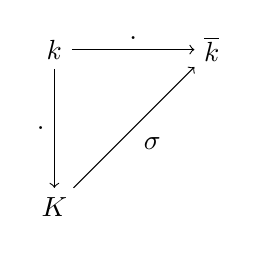
\begin{tikzpicture}[node distance=2cm, auto]
		\node (k) {$k$};
		\node (kk) [right of=k] {$\overline{k}$};
		\node (K) [below of=k] {$K$};

		\draw[->] (k) to node {$.$} (kk);
		\draw[->] (k) to node[swap] {$.$} (K);
		\draw[->] (K) to node[swap] {$\sigma$} (kk);

	\end{tikzpicture}
	\end{figure}

	\item $K$ é corpo de raízes sobre $k$ de uma família $(f_i)_{i \in I}$ de polinômios em $k[x] \setminus k$;
	\item Se $f \in k[x] \setminus k$ é irredutível em $k[x]$ com raiz $\alpha$, então $f(x)=c(x-\alpha_1)\cdots(x-\alpha_n)$ em $k[x]$, com $\alpha_1=\alpha$ e $c \in k \setminus \{0\}$.
	\end{enumerate}
\end{theorem}
%\begin{proof}
%PULEI, tem nas notas mas não tudo.
%\end{proof}

\begin{definition}
	Uma extensão de corpos $k \subseteq K$ é uma \emph{extensão normal} se ela satisfaz uma das três condições do teorema acima.
\end{definition}

OBS: Se $k \subseteq \overline{k}$ é uma extensão algébrica, então todo $\beta \in \overline{k}$ é algébrico sobre $k$ vale para $\beta \in K$, então $k \subseteq K$ é extensão algébrica.

	Se $k \subseteq K$ é extensão algébrica, então $k \subseteq K \subseteq \overline{K}$ são extensões algébricas, então $k \subseteq \overline{K}$ é extensão algébrica. Então $\overline{k} \sim \overline{K}$ é fecho algébrico de $k$.

%(?????)

\begin{proposition}
	Seja $k \subseteq K$ um extensão algébrica e $\sigma: K \to K$ um homomorfismo de corpos que satisfaz $\sigma|_k=id|_k$. Então $\sigma$ é um isomorfismo de corpos.
\end{proposition}
%\begin{proof}
%...
%\end{proof}

\begin{definition}
	Seja $E \subseteq F$ uma extensão algébrica e $\sigma:E \to L$ um homomorfismo de corpos tal que $L$ é algebricamente fechado, $\sigma(E) \subseteq L$ é uma extensão algébrica ($L$ é fecho algébrico de $\sigma(E)$)
	\begin{equation*}
	S_\sigma := \{\mu : \mu: F \to L \text{\ homomorfismo de corpos}, \mu|_E=\sigma\}.
	\end{equation*}
\end{definition}

\begin{lemma}
	$|S_\sigma|$ depende de $E \subseteq F$, mas não depende de $\sigma$ nem de $L$.
\end{lemma}
%\begin{proof}
%... vários diagramas
%\end{proof}

\begin{definition}
	Seja $E \subseteq F$ uma extensão algébrica. O \emph{grau de separabilidade} da extensão é $[F:E]_S := |S_\sigma|$. (Pode escolher $l=\overline{E}$ e $\sigma$ inclusão.)
\end{definition}

\begin{theorem}
	\begin{enumerate}
	\item $E \subseteq F \subseteq K$ extensões algébricas, então
		\begin{equation*}
		[K:E]_S = [K:F]_S[F:E]_S
		\end{equation*}
	\item $E \subseteq F$ extensão finita (logo algébrica), então
		\begin{equation*}
		[F:E]_S \leq [F:E]
		\end{equation*}
	\end{enumerate}
\end{theorem}
%\begin{proof}
%...
%\end{proof}

\begin{definition}
	Seja $E \subseteq K$ uma extensão finita. Ela é \emph{separável} se $[K:E]_S=[K:E]$.
\end{definition}

\begin{corollary}
	Sejam $E \subseteq F \subseteq K$ extensões de corpos, $[K:E] < \infty$, $E \subseteq K$ separável. Então $E \subseteq F$ e $F subseteq K$ são separáveis.
\end{corollary}
\begin{proof}
	\begin{equation*}
	[K:F]_S [F:E]_S = [K:E]_S = [K:E] = [K:F][F:E].
	\end{equation*}
	Como $[F:E]_S \leq [F:E]$ e $[K:F]_S \leq [K:F]$, segue o corolário.
\end{proof}



\section{Ação de anel}
\label{sec:aneis.acao}

Consideramos brevemente ações de anéis em grupos comutativos. Na definição usamos o fato de que, se $\bm G$ é um grupo comutativo, $\Homo(\bm G)$ é um anel com as operações puxadas para o espaço de funções, a soma pontual sendo a soma do anel e a composição de função sendo o produto. De fato, se $X$ é um conjunto e $\bm G$ um grupo comutativo, o conjunto $\Func(X,G)$ de funções de $X$ para $G$, com a soma pontual e a composição, é um anel, e basta mostrar que quando $X=G$, o conjunto $\Homo(\bm G)$ de endomorfismos de grupo de $\bm G$ é um subanel de $\Func(G)$.
Demonstramos isso a seguir.

\subsection{Anel de endomorfismos de grupo}

\begin{proposition}
Sejam $X$ um conjunto e $\bm G$ um grupo comutativo. Então
	\begin{equation*}
	\bm{\Func}(X,\bm G) := (\Func(X,G),+,-,0,\circ,\Id)
	\end{equation*}
é um anel\footnote{No sentido em que a multiplicação $\circ$ não precisa ser comutativa.}.
\end{proposition}
\begin{proof}
	\begin{enumerate}
	\item $(\Func(X,G),+,-,0)$ é um grupo comutativo.
		\begin{enumerate}
		\item Para todos $f_0,f_1,f_2 \in \Func(X,G)$ e $x \in X$,
			\begin{align*}
			((f_0+f_1)+f_2)(x) &= (f_0+f_1)(x)+f_2(x) \\
				&= (f_0(x)+f_1(x))+f_2(x) \\
				&= f_0(x)+(f_1(x)+f_2(x)) \\
				&= f_0(x)+(f_1+f_2)(x) \\
				&= (f_0+(f_1+f_2))(x);
			\end{align*}
		\item Para todos $f \in \Func(X,G)$ e $x \in X$,
			\begin{align*}
			(0+f)(x) &= 0(x)+f(x) \\
				&= 0+f(x) \\
				&= f(x) \\
				&= f(x)+0 \\
				&= f(x)+0(x) \\
				&= (f+0)(x);
			\end{align*}
		\item Para todos $f \in \Func(X,G)$ e $x \in X$,
			\begin{align*}
			((-f)+f)(x) &= (-f)(x)+f(x) \\
				&= -f(x)+f(x) \\
				&= 0 \\
				&= f(x)+(-f(x)) \\
				&= f(x) + (-f)(x) \\
				&= (f+(-f))(x);				
			\end{align*}
		\item Para todos $f_0,f_1 \in \Func(X,G)$ e $x \in X$,
			\begin{align*}
			(f_0+f_1)(x) = f_0(x)+f_1(x) = f_1(x) + f_0(x) = (f_1+f_0)(x).
			\end{align*}
		\end{enumerate}
	
	\item $(\Func(X,G),\circ,\Id)$ é um monoide.
		\begin{enumerate}
		\item Para todos $f_0,f_1,f_2 \in \Func(X,G)$ e $x \in X$,
			\begin{align*}
			((f_0 \circ f_1) \circ f_2)(x) &= (f_0 \circ f_1)(f_2(x)) \\
				&= (f_0(f_1(f_2(x))) \\
				&= f_0((f_1 \circ f_2)(x)) \\
				&= (f_0 \circ (f_1 \circ f_2))(x);
			\end{align*}
		\item Para todos $f \in \Func(X,G)$ e $x \in X$,
			\begin{align*}
			(\Id \circ f)(x) = \Id(f(x)) = f(x) = f(\Id(x)) = (f \circ \Id)(x).
			\end{align*}
		\end{enumerate}
	\item A composição $\circ$ é distributiva à esquerda e à direita sobre a soma pontual $+$.
		\begin{enumerate}
		\item Para todos $f,f_0,f_1 \in \Func(X,G)$ e $x \in X$,
			\begin{align*}
			(f \circ (f_0+f_1))(x) &= f((f_0+f_1)(x)) \\
				&= f(f_0(x)+f_1(x)) \\
				&= f(f_0(x))+f(f_1(x)) \\
				&= (f \circ f_0)(x) + (f \circ f_1)(x);
			\end{align*}
		\item Para todos $f_0,f_1,f \in \Func(X,G)$ e $x \in X$,
			\begin{align*}
			((f_0+f_1) \circ f)(x) &= (f_0+f_1)(f(x)) \\
				&= f_0(f(x)) + f_1(f(x)) \\
				&= (f_0 \circ f)(x) + (f_1 \circ f)(x).
			\end{align*}
		\end{enumerate}
	\end{enumerate}
\end{proof}

\begin{proposition}
Seja $\bm G$ um grupo comutativo. Então
	\begin{equation*}
	\bm{\Homo}(\bm G) := (\Homo(\bm G),+,-,0,\circ,\Id)
	\end{equation*}
é um anel\footnote{No sentido em que a multiplicação $\circ$ não precisa ser comutativa.}.
\end{proposition}
\begin{proof}
Como $\Homo(\bm G) \subseteq \Func(G)$, basta mostrar que $\Homo(\bm G)$ é subanel de $\bm{\Func}(\bm G)$.
	\begin{enumerate}
	\item $(\Homo(\bm G),+,-,0)$ é subgrupo.
		\begin{enumerate}
		\item Para todos $h_0,h_1 \in \Homo(\bm G)$ e $g_0,g_1 \in G$,
			\begin{align*}
			(h_0+h_1)(g_0+g_1) &= h_0(g_0+g_1) + h_1(g_0+g_1) \\
				&= h_0(g_0) + h_0(g_1) + h_1(g_0) + h_1(g_1) \\
				&= h_0(g_0) + h_1(g_0) + h_0(g_1) + h_1(g_1) \\
				&= (h_0 + h_1)(g_0) + (h_0 + h_1)(g_1);
			\end{align*}
		\item Para todos $h \in \Homo(\bm G)$ e $g_0,g_1 \in G$,
			\begin{align*}
			(-h)(g_0+g_1) &= -h(g_0+g_1) \\
				&= -(h(g_0)+h(g_1)) \\
				&= -h(g_0)-h(g_1) \\
				&= (-h)(g_0)+(-h)(g_1).
			\end{align*}
		\end{enumerate}
	\item $(\Homo(\bm G),\circ,\Id)$ é submonoide.
		\begin{enumerate}
		\item Para todos $h_0,h_1 \in \Homo(\bm G)$ e $g_0,g_1 \in G$,
			\begin{align*}
			(h_0 \circ h_1)(g_0+g_1) &= h_0(h_1(g_0+g_1)) \\
				&= h_0(h_1(g_0)+h_1(g_1)) \\
				&= h_0(h_1(g_0))+h_0(h_1(g_1)) \\
				&= (h_0 \circ h_1)(g_0)+h_0 \circ h_1)(g_1);
			\end{align*}
		\item Para todos $g_0,g_1 \in G$,
			\begin{align*}
			\Id(g_0+g_1) = g_0+g_1 = \Id(g_0)+\Id(g_1).
			\qedhere
			\end{align*}
		\end{enumerate}
	\end{enumerate}
\end{proof}

\begin{definition}
Sejam $\bm A$ um anel e $\bm G$ um grupo comutativo. Uma \emph{ação} de $\bm A$ sobre $\bm G$ é um homomorfismo de anel
	\begin{align*}
	\func{\bm \cdot}{A}{\Homo(\bm G)}{a}{
		\begin{aligned}[t]
		\func{a \bm \cdot}{G}{G}{g}{a \bm \cdot g}.
		\end{aligned}
	}
	\end{align*}
Denota-se $\acao{\bm \cdot}{\bm A}{\bm G}$. Diz-se que o anel $\bm A$ \emph{age} no grupo $\bm G$ e denota-se $\bm A \age \bm G$ se, e somente se, existe ação de $\bm A$ em $\bm G$.
\end{definition}

Se denotamos $\bm A=(A,+,-,0,\times,1)$ e $\bm G = (G,\bm +,\bm -, \bm 0)$, essa definição é equivalente às seguintes propriedades.
	\begin{enumerate}
	\item  Para todo $a \in A$, a função $\fun{a \bm \cdot}{G}{G}$ é um homomorfismo de grupo:
		\begin{enumerate}
		\item Para todos $a \in A$ e $g,g' \in G$,
			\begin{equation*}
			a \bm \cdot (g \bm + g') = a \bm \cdot g \bm + a \bm \cdot g'.
			\end{equation*}
		\end{enumerate}
	\item $\fun{\bm \cdot}{\bm A^+}{(\Homo(\bm G),\bm +,\bm -,\bm 0)}$ é homomorfismo de grupo:
		\begin{enumerate}
		\item Para todos $a,a' \in A$ e $g \in G$,
			\begin{equation*}
			(a + a') \bm \cdot m = a \bm \cdot g + a' \bm \cdot g;
			\end{equation*}
		\end{enumerate}
	\item  $\fun{\bm \cdot}{\bm A^\times}{(\Homo(\bm G),\circ,\Id)}$ é homomorfismo de monoide:
		\begin{enumerate}
		\item Para todos $a,a' \in A$ e $g \in G$,
			\begin{equation*}
			(a \times a') \bm \cdot g = a \bm \cdot (a' \bm \cdot g);
			\end{equation*}
		\item Para todo $g \in G$,
			\begin{equation*}
			1 \bm \cdot g = g.
			\end{equation*}
		\end{enumerate}
	\end{enumerate}
\chapter{Módulos}

\section{Módulos e submódulos}

\begin{definition}
Seja $\bm A=(A,+,-,0,\times,1)$ um anel. Um \emph{módulo} sobre $\bm A$ é uma lista $\bm M = (M,\bm +,\bm -,\bm 0,\pt)$ em que $\bm M^+ := (M,\bm +,\bm -,\bm 0)$ é um grupo comutativo e $\acao{\pt}{\bm A}{\bm M^+}$ é uma ação de anel ($\fun{\pt}{\bm A}{\bm{\Homo}(\bm M^+)}$ é um homomorfismo de anel); ou seja,
	\begin{enumerate}
	\item Para todos $a \in A$ e $m,m' \in M$,
		\begin{equation*}
		a \pt (m \bm + m') = a \pt m \bm + a \pt m'.
		\end{equation*}
	\item Para todos $a,a' \in A$ e $m \in M$,
		\begin{equation*}
		(a + a') \pt m = a \pt m + a' \pt m;
		\end{equation*}
	\item Para todos $a,a' \in A$ e $m \in M$,
		\begin{equation*}
		(a \times a') \pt m = a \pt (a' \pt m);
		\end{equation*}
	\item Para todo $m \in M$,
		\begin{equation*}
		1 \pt m = m.
		\end{equation*}
	\end{enumerate}
Os símbolos `$\times$' da multiplicação de $\bm A$ e `$\pt$' da ação de $\bm A$ sobre $\bm M$ serão suprimidos (e parênteses desnecessários relacionados a elas também), e os símbolos `$\bm +$', `$\bm -$' e `$\bm 0$' das operações de $\bm M$ não serão diferenciados em notação dos símbolos `$+$', `$-$' e `$0$' das operações de $\bm A$.
\end{definition}

Na definição usamos o fato de que $\bm{\Homo}(\bm M^+) = (\Homo(\bm M^+),+,-,0,\circ,\Id)$ é um anel com as operações puxadas para o espaço de funções, a soma pontual sendo a soma do anel e a composição de função sendo o produto. Isso foi feito em \cref{sec:aneis.acao}.

\begin{example}
Sejam $\bm A=(A,+,-,0,\times,1)$ um anel e $I \ide A$ um ideal. Então $\bm I = (I,+,-,0,\pt)$ é um módulo sobre $\bm A$, em que $\bm I^+ = (I,+,-,0)$ é o subgrupo aditivo de $\bm A$ e
	\begin{align*}
	\func{\pt}{A}{\Homo(I)}{a}{
		\begin{aligned}[t]
			\func{a \pt}{I}{I}{i}{ai}
		\end{aligned}
	}
	\end{align*}
é a ação multiplicativa induzida pela multiplicação $\times$ de $\bm A$. Note que, para cada $a \in A$, a função $\fun{a \pt}{I}{I}$ está bem definida pois $I$ é um ideal, o que implica que, para todo $i \in I$, $ai \in I$.
\end{example}

\begin{example}
Seja $\bm G=(G,+,-,0)$ um grupo comutativo. Então
	\begin{equation*}
	(G,+,-,0,\pt)
	\end{equation*}
é um módulo sobre $\Z$, em que
	\begin{align*}
	\func{\pt}{\Z}{\Homo(G)}{n}{
		\begin{aligned}[t]
			\func{n \pt}{G}{G}{g}{ng=\sum_{i \in [n]} g}.
		\end{aligned}
	}
	\end{align*}
\end{example}

\begin{exercise}
Seja $\bm M$ um módulo sobre um anel $\bm A$.
	\begin{enumerate}
	\item Para todo $a \in A$, $a0=0$;
	\item Para todo $m \in M$, $0m=0$;
	\item Para todos $a \in A$ e $m \in M$, $-(am)=(-a)m=a(-m)$.
	\end{enumerate}
\end{exercise}

\begin{definition}
Seja $\bm M$ um módulo sobre um anel $\bm A$. Um submódulo de $\bm M$ sobre $\bm A$ é uma lista $\bm S = (S,+,-,0,\pt)$ tal que
	\begin{enumerate}
	\item $\bm S^+ := (S,+,-,0)$ é um subgrupo de $\bm M^+$;
	\item Para todos $a \in A$ e $m \in S$, $am \in S$.
	\end{enumerate}
\end{definition}

\section{Homomorfismo de módulo}

\begin{definition}
Sejam $\bm M$ e $\bm M'$ módulos sobre um anel $\bm A$. Um \emph{homomorfismo de módulo} de $\bm M$ para $\bm M'$ é uma função $\fun{h}{M}{M'}$ tal que
	\begin{enumerate}
	\item (Aditividade) A função $\fun{h}{\bm M^+}{\bm {M'}^+}$ é um homomorfismo de grupo: para todos $m_0,m_1 \in M$,
		\begin{equation*}
		h(m_0 + m_1) = h(m_0) + h(m_1);
		\end{equation*}

	\item (Homogeneidade) %(Comutatividade com ação)
	Para todos $a \in A$, $m \in M$,
		\begin{equation*}
		h(a m) = a h(m).
		\end{equation*}
	\end{enumerate}
Denota-se $\fun{h}{\bm M}{\bm M'}$. O conjunto dos homomorfismos de módulo de $\bm M$ para $\bm M'$ é denotado $\Homo(\bm M, \bm M')$. Um \emph{endomorfismo} de módulo de $\bm M$ é um homomorfismo de módulo de $\bm M$ para $\bm M$. O conjunto dos endomorfismos de módulo de $\bm M$ é denotado $\Homo(\bm M)$.
\end{definition}

\begin{exercise}[Composição de homomorfismos]
Sejam $\bm M$ , $\bm M'$ e $\bm M''$ módulos sobre um anel $\bm A$, $h \in \Homo(\bm M, \bm M')$ e $h' \in \Homo(\bm M', \bm M'')$ homomorfismos. Então $h' \circ h \in  \Homo(\bm M, \bm M'')$.
\end{exercise}

\subsection{Módulo de homomorfismos de módulo}

Por definição de homomorfismo de módulo, temos que
	\begin{equation*}
	\Homo(\bm M,\bm M') \subseteq \Homo(\bm M^+,{\bm M'}^+),
	\end{equation*}
ou seja, que todo homomorfismo de módulo é em particular um homomorfismo de grupo entre as estruturas de grupo $\bm M^+$ e ${\bm M'}^+$ de seus respectivos módulos. O conjunto de homomorfismos de grupo $\Homo(\bm M^+,{\bm M'}^+)$ é um grupo com a adição, subtração e função nula puxadas das respectivas operações de ${\bm M'}^+$. Dotado dessa estrutura de grupo, o conjunto $\Homo(\bm M,\bm M')$ é de fato um subgrupo de $\Homo(\bm M^+,{\bm M'}^+)$, que denotamos por
	\begin{equation*}
	\bm{\Homo}(\bm M,\bm M')^+ := (\Homo(\bm M,\bm M'),+,-,0).
	\end{equation*}

\begin{proposition}
\label{prop:mod.subgrupo}
Sejam $\bm M$ e $\bm M'$ módulos sobre um anel $\bm A$.
%	\begin{equation*}
%	(\Homo(\bm M,\bm M'),+,-,0) \leq (\Homo(\bm M^+,{\bm M'}^+),+,-,0).
%	\end{equation*}
	\begin{equation*}
	\bm{\Homo}(\bm M,\bm M')^+ \leq \bm{\Homo}(\bm M^+,{\bm M'}^+).
	\end{equation*}
\end{proposition}
\begin{proof}
	\begin{enumerate}
	\item (Não vacuidade) A função nula
		\begin{align*}
		\func{0}{M}{M'}{m}{0}
		\end{align*}
	é um homomorfismo de módulo de $\bm M$ para $\bm M'$:
		\begin{enumerate}
		\item (Aditividade) Segue direto de $0 \in \Homo(\bm M^+,{\bm M'}^+)$;
		\item (Homogeneidade) Para todos $a \in A$, $m \in M$,
			\begin{equation*}
			h(a m) = 0 = a0 = ah(m).
			\end{equation*}
		\end{enumerate}

	\item (Fechamento) Para todos $h,h' \in \Homo(\bm M,\bm M')$, $h+h' \in \Homo(\bm M,\bm M')$:
		\begin{enumerate}
		\item (Aditividade) Segue direto de $h+h' \in  \Homo(\bm M^+,{\bm M'}^+)$;
		\item (Homogeneidade) Para todos $a \in A$, $m \in M$,
			\begin{align*}
			(h+h')(am) &= h(am) + h'(am) \\
				&= ah(m) + ah'(m) \\
				&= a(h(m) + h'(m)) \\
				&= a(h+h')(m).
			\end{align*}
		\end{enumerate}

	\item (Invertibilidade) Para todo $h \in \Homo(\bm M,\bm M')$, $-h \in \Homo(\bm M,\bm M')$:
		\begin{enumerate}
		\item (Aditividade) Segue direto de $-h \in  \Homo(\bm M^+,{\bm M'}^+)$;
		\item (Homogeneidade) Para todos $a \in A$, $m \in M$,
			\begin{equation*}
			(-h)(am) = -h(am) = -(ah(m)) = a(-h(m)).
			\end{equation*}
		\end{enumerate}
	\end{enumerate}
\end{proof}

\begin{definition}
Sejam $\bm M$ e $\bm M'$ módulos sobre um anel $\bm A$. O \emph{módulo de homomorfismos} de $\bm M$ para $\bm M'$ é a lista
	\begin{equation*}
	\bm{\Homo}(\bm M, \bm M') := (\Homo(\bm M, \bm M'),+,-,0,\pt)
	\end{equation*}
em que
	\begin{enumerate}
	\item $\Homo(\bm M, \bm M')$ é o conjunto dos homomorfismo de módulo de $\bm M$ para $\bm M'$;

	\item $\bm{\Homo}(\bm M,\bm M')^+ = (\Homo(\bm M,\bm M'),+,-,0)$ é o grupo de homomorfismos de módulo, com as operações definidas pontualmente, induzidas das operações de $\bm M'$;

	\item $\pt$ é a ação induzida
		\begin{align*}
		\func{\pt}{A}{\Homo(\bm{\Homo}(\bm M,\bm M')^+)}{a}{
			\begin{aligned}[t]
			\func{a \pt}{\Homo(\bm M,\bm M')}{\Homo(\bm M,\bm M')}{h}{
				\begin{aligned}[t]
				\func{a \pt h}{M}{M'}{g}{a \pt h(g)}.
				\end{aligned}
			}
			\end{aligned}
		}
		\end{align*}
	\end{enumerate}
\end{definition}

Note que a ação é induzida pela ação de $\bm M'$, que é a ação que aparece na expressão $a \pt h(g)$. Na expressão $\Homo(\bm{\Homo}(\bm M,\bm M')^+)$, o `$\bm{\Homo}$' interno se refere ao grupo de homomorfismos do módulo, subgrupo do grupo de homomorfismos do grupo comutativo $\bm M^+$ para o grupo comutativo ${\bm M'}^+$, enquanto o `$\Homo$' externo se refere ao conjunto de endomorfismos do grupo $\Homo(\bm M,\bm M')$.

\begin{proposition}
Sejam $\bm M$ e $\bm M'$ módulos sobre um anel $\bm A$. O módulo de homomorfismos de $\bm M$ para $\bm M'$ é um módulo sobre $\bm A$.
\end{proposition}
\begin{proof}
Foi provado em \ref{prop:mod.subgrupo} que $\bm{\Homo}(\bm M,\bm M')^+$ é grupo comutativo, pois é subgrupo de $\bm{\Homo}(\bm M^+,{\bm M'}^+)$.

Devemos provar que $\acao{\pt}{\bm A}{\bm{\Homo}(\bm M,\bm M')^+}$ é ação de anel:
	\begin{enumerate}
	\item Para todos $a \in A$, $h,h' \in \Homo(\bm M,\bm M')$ e $m \in M$,
		\begin{align*}
		(a \pt (h+h'))(m) &= a \pt (h+h')(m) \\
			&= a \pt (h(m) + h'(m)) \\
			&= a \pt h(m) + a \pt h'(m) \\
			&= (a \pt h + a \pt h')(m);
		\end{align*}
	\item Para todos $a,a' \in A$, $h \in \Homo(\bm M,\bm M')$ e $m \in M$,
		\begin{align*}
		((a+a') \pt h)(m) &= (a+a') \pt h(m) \\
			&= a \pt h(m) + a' \pt h(m) \\
			&= (a \pt h + a' \pt h)(m);
		\end{align*}
	\item Para todos $a,a' \in A$, $h \in \Homo(\bm M,\bm M')$ e $m \in M$,
		\begin{align*}
		((aa') \pt h)(m) &= (aa') \pt h(m) \\
			&= a \pt (a' \pt h(m)) \\
			&= a \pt ((a' \pt h)(m)) \\
			&= (a \pt (a' \pt h))(m);
		\end{align*}
	\item Para todos $h \in \Homo(\bm M,\bm M')$ e $m \in M$,
		\begin{equation*}
		(1 \pt h)(m) = 1 \pt h(m) = h(m).
		\qedhere
		\end{equation*}
	\end{enumerate}
\end{proof}





\chapter{Espaços lineares}

\section{Espaço e subespaço lineares}

\begin{definition}
Seja $\bm C=(C,+,-,0,\cdot,1)$ um corpo. Um \emph{espaço linear} sobre $\bm C$ é um módulo $(\bm V,\bm \cdot)$ sobre $\bm C$; ou seja,
	\begin{enumerate}
	\item  Para todo $c \in C$, a função $c \bm \cdot \colon \bm V \to \bm V$ é um homomorfismo de grupo:
		\begin{enumerate}
		\item Para todos $v_0,v_1 \in M$,
			\begin{equation*}
			c \bm \cdot (v_0 \bm + v_1) = c \bm \cdot v_0 \bm + c \bm \cdot v_1.
			\end{equation*}
		\end{enumerate}
	\item $\bm \cdot \colon C \times V \to V$ é uma ação de corpo (ou de anel):
		\begin{enumerate}
		\item Para todos $c_0,c_1 \in C$ e $v \in V$,
			\begin{equation*}
			(c_0 + c_1) \bm \cdot v = c_0 \bm \cdot v + c_1 \bm \cdot v;
			\end{equation*}
		\item Para todos $c_0,c_1 \in C$ e $v \in V$,
			\begin{equation*}
			(c_0 \cdot c_1) \bm \cdot v = c_0 \bm \cdot (c_1 \bm \cdot v);
			\end{equation*}
		\item Para todo $v \in V$,
			\begin{equation*}
			1 \bm \cdot v = v;
			\end{equation*}
		\end{enumerate}
	\end{enumerate}
Os símbolos da operação $\cdot$ de $\bm C$ e da ação $\bm \cdot$ serão suprimidos (e parênteses desnecessários relacionados a elas também), e os símbolos das operações $+,-$ de $\bm C$ e $\bm +,\bm -$ de $\bm V$ não serão diferenciadas em notação.
%, nem os das constantes $0 \in C$ e $\bm 0 \in V$.
Um espaço linear será denotado como $\bm V$ quando não for relevante explicitar a ação $\bm \cdot$.
\end{definition}

%\begin{definition}
%Um \emph{espaço linear} (ou \emph{espaço vetorial}) sobre um corpo $\bm C=(C,+,\cdot)$ é um módulo $\bm V=(\bm V, \bm \cdot)$ sobre $\bm C$; mais detalhadamente, é uma tripla $\bm V = (V, \bm +, \bm \cdot)$ em que
%	\begin{enumerate}
%	\item $(V,\bm +)$ é um grupo comutativo com elemento neutro $\bm 0$;
%	\item $\bm \cdot: C \times V \to V$ é uma função que satisfaz
%		\begin{enumerate}
%		\item $\forall \bm v \in V \qquad 1\bm\cdot \bm v=\bm v$;
%		\item $\forall c_1,c_2 \in C \ \forall \bm v \in V \qquad (c_1 \cdot c_2) \bm\cdot \bm v = c_1 \bm\cdot(c_2 \bm\cdot \bm v)$;
%		\item $\forall c \in C \ \forall \bm v_1,\bm v_2 \in V \qquad c \bm\cdot (\bm v_1 \bm + \bm v_2) = c \bm\cdot \bm v_1 \bm + c\bm\cdot \bm v_2$;
%		\item $\forall c_1,c_2 \in C \ \forall \bm v \in V \qquad (c_1+c_2) \bm\cdot \bm v = c_1 \bm{\cdot v} \bm + c_2\bm{\cdot v}$.
%		\end{enumerate}
%	\end{enumerate}
%Os elementos de $V$ são \emph{vetores} e denotados em negrito e os elementos de $C$ são \emph{escalares}. As operações $\bm +$ e $\bm \cdot$ do espaço linear são denotadas por $+$ e $\cdot$, o inverso de $\bm v \in V$ é denotado $-\bm v$ e a imagem de $(c,\bm v) \in C \times V$ é o \emph{produto} de $c$ e $\bm v$ e é denotada por $c\bm v$. Quando o corpo é $\R$, dizemos \emph{espaço vetorial real}; quando o corpo é $\C$, dizemos \emph{espaço vetorial complexo}.
%\end{definition}

\begin{proposition}
Seja $\bm V$ um espaço linear sobre um corpo $\bm C$. Para todos $\bm v \in V$ e $c \in C$,
	\begin{enumerate}
	\item $c\bm v = \bm 0 \Leftrightarrow c=0 \text{\ \ ou\ \ } \bm v = \bm 0$;
	\item $-(c\bm v) = (-c)\bm v = c(- \bm v)$;
	\item $c\bm v = (-c)(- \bm v)$.
	\end{enumerate}
\end{proposition}
\begin{proof} Sejam $\bm v \in V$ e $c \in C$.
	\begin{enumerate}
	\item Primeiro, notemos que
		\begin{align*}
		0 \bm v &= 0 \bm v + \bm 0 \\
			&= 0 \bm v + (0 \bm v - 0 \bm v) \\
			&= (0 \bm v + 0 \bm v) - 0 \bm v \\
			&= (0+0) \bm v - 0 \bm v \\
			&= 0 \bm v - 0 \bm v \\
			&= \bm 0.
		  \end{align*}
Agora, notemos que
		\begin{align*}
		c \bm 0 &= c \bm 0 + \bm 0 \\
			&= c \bm 0 + (c \bm 0 - c \bm 0) \\
			&= (c \bm 0 + c \bm 0) - c \bm 0 \\
			&= c  (\bm 0 + \bm 0) - c \bm 0 \\
			&= c \bm 0 - c \bm 0 \\
			&= \bm 0.
		\end{align*}
Portanto, se $c=0$ ou $\bm v = \bm 0$, então $c\bm v = \bm 0$. Agora, suponhamos que $c\bm v =\bm 0$. Se $c \neq 0$, como $\bm C$ é corpo, segue da demonstração anterior que
		\begin{equation*}
		\bm v = c^{-1}c\bm v = c^{-1} \bm 0 = \bm 0.
		\end{equation*}
	\item Basta notar que
		\begin{align*}
		\bm -(c\bm{v}) &= \bm -(c\bm{v}) + \bm 0 \\
			&= \bm -(c\bm{v}) + (0 \bm v) \\
			&= \bm -(c\bm{v}) + (c-c) \bm v \\
			&= \bm -(c\bm{v}) + (c\bm v + (-c) \bm v) \\
			&= (\bm -(c\bm{v}) + c\bm v) + (-c) \bm v \\
			&= \bm 0 + (-c) \bm v \\
			&= (-c) \bm v
		\end{align*}
e que
		\begin{align*}
		-(c\bm{v}) &= -(c\bm{v}) + \bm 0 \\
			&= -(c\bm v) + (c \bm 0) \\
			&= -(c\bm v) + c(\bm v - \bm v) \\
			&= -(c\bm v) + (c\bm v + c(- \bm v)) \\
			&= (-(c\bm v + c\bm v) + c(- \bm v) \\
			&= \bm 0 + c(- \bm v) \\
			&= c(- \bm v).
		\end{align*}
	\item Do item anterior, segue que
		\begin{equation*}
		c\bm v = (-(-c))\bm v = (-c)(- \bm v).  \qedhere
		\end{equation*}
	\end{enumerate}
\end{proof}

\begin{proposition}
Seja $\bm C$ um corpo e $n$ um natural positivo. Então $(C^n,+,\bm\cdot)$, em que
	\begin{align*}
	\func{\bm\cdot}{C \times C^n}{C^n}{(c,(c_1,\ldots,c_n))}{(c \cdot c_1,\ldots,c \cdot c_n),}
	\end{align*}
é um espaço vetorial sobre $\bm C$.
\end{proposition}
\begin{proof}
	Claramente $(C^n,+)$ é um grupo comutativo com elemento neutro $(0,\ldots,0)$. Note que, para todos $(c_1,\ldots,c_n) \in C^n$ e $c,c' \in C$,
	\begin{equation*}
	1 \bm\cdot (c_1,\ldots,c_n) = (1 \cdot c_1,\ldots,1 \cdot c_n) = (c_1,\ldots,c_n)
	\end{equation*}
e
	\begin{align*}
	(c \cdot c') \bm\cdot (c_1,\ldots,c_n) &= ((c \cdot c') \cdot c_1, \ldots, (c \cdot c') \cdot c_n) \\
	&= ((c \cdot (c' \cdot c_1), \ldots, (c \cdot (c' \cdot c_n)) \\
	&= c \bm\cdot (c' \cdot c_1,\ldots,c' \cdot c_n) \\
	&= c \bm\cdot (c' \bm\cdot (c_1,\ldots,c_n)).
	\end{align*}
	Ainda, note que, para todos $(c_1,\ldots,c_n), (c'_1,\ldots,c'_n) \in C^n$ e $c,c' \in C$,
	\begin{align*}
	c \bm\cdot ((c_1,\ldots,c_n) + (c'_1,\ldots,c'_n)) &= c \bm\cdot (c_1+c'_1,\ldots,c_n+c'_n) \\
	&= (c \cdot (c_1+c'_1),\ldots,c \cdot (c_n+c'_n)) \\
	&= (c \cdot c_1 + c \cdot c'_1,\ldots,c \cdot c_n + c \cdot c'_n) \\
	&= (c \cdot c_1,\ldots,c \cdot c_n) + (c \cdot c'_1,\ldots,c \cdot c'_n) \\
	&= c \bm\cdot (c_1,\ldots,c_n) + c \bm\cdot (c'_1,\ldots,c'_n)
	\end{align*}
e
	\begin{align*}
	(c+c') \bm\cdot (c_1,\ldots,c_n) &= ((c+c')c_1,\ldots,(c+c')c_n) \\
	&= (c \cdot c_1 + c' \cdot c_1,\ldots,c \cdot c_n + c' \cdot c_n)_{i \in I} \\
	&= (c \cdot c_1,\ldots,c \cdot c_n) + (c' \cdot c_1,\ldots,c' \cdot c_n) \\
	&= c \bm\cdot (c_1,\ldots,c_n) + c' \bm\cdot (c_1,\ldots,c_n).  \qedhere
	\end{align*}
\end{proof}

Para generalizar esse resultado, lembremos que o produto de uma família $(C_i)_{i \in I}$ de conjuntos é $\prod_{i \in I} C_i$ e, quando $C_i=C$, temos que $\prod_{i \in I} C_i = C^I$ e os elementos de $C^I$ são funções $c=(c_i)_{i \in I}$ de $I$ em $C$.

\begin{proposition}
Sejam $I$ um conjunto e $\bm C$ um corpo. Então $\bm {C^I}=(C^I,\bm +,\bm\cdot)$, em que
	\begin{align*}
	\func{\bm +}{C^I}{C^I}{(\bm c,\bm c')}{(c_i+c'_i)_{i \in I}}
	\end{align*}
e
	\begin{align*}
	\func{\bm\cdot}{C \times C^I}{C^I}{(a,\bm c)}{(a \cdot c_i)_{i \in I}}
	\end{align*}
é um espaço vetorial sobre $\bm C$.
\end{proposition}

Esse exemplo pode ser ainda mais generalizado como a seguir.

%%%%%%%%%%%%%%%%%%%%%%%%%%%%%%%%%%%%%%%%%%%%
\begin{comment}
\begin{proposition}[Espaço de Funções]
Sejam $\bm V$ e $\bm W$ espaços vetoriais sobre um corpo $\bm C$. Então $\bm{W^V}=(W^V,+,\cdot)$, em que
	\begin{align*}
	\func{+}{W^V \times W^V}{W^V}{(\bm f_1,\bm f_2)}{
		\begin{aligned}[t]
		\func{\bm f_1+\bm f_2}{V}{W}{\bm v}{\bm f_1(\bm v)+\bm f_2(\bm v).}
		\end{aligned}
	}
	\end{align*}
e
\begin{align*}
	\func{\cdot}{C \times W^V}{W^V}{(c,\bm f)}{
		\begin{aligned}[t]
		\func{c\bm f}{V}{W}{\bm v}{c\bm f(\bm v),}
		\end{aligned}
	}
	\end{align*}
é um espaço vetorial sobre $\bm C$.
\end{proposition}
\begin{proof}
Primeiro, sabemos que $(W^V,+)$ é um grupo comutativo com identidade $0: W^V \times W^V \to W^V$ definida por $0(\bm v)=0$. Devemos então mostrar que $\cdot: C \times W^V \to W^V$ satisfaz os itens da definição de espaço vetorial. Primeiro, seja $\bm f \in W^V$. Então, para todo $\bm v \in V$, $(1\bm f)(\bm v)=1\bm f(\bm v)=\bm f(\bm v)$, o que mostra que $1\bm f=\bm f$. Agora, sejam $c_1,c_2 \in C$ e $\bm f \in W^V$. Então, para todo $\bm v \in V$,
	\begin{equation*}
	((c_1c_2)\bm f)(\bm v) = (c_1c_2)\bm f(\bm v) = c_1(c_2\bm f(\bm v)) = c_1(c_2\bm f)(\bm v) = (c_1(c_2\bm f))(\bm v),
	\end{equation*}
o que mostra que $(c_1c_2)\bm f=c_1(c_2\bm f)$.

Por fim, devemos mostrar as propriedades distributivas. Sejam $c \in C$ e $\bm f_1,\bm f_2 \in W^V$. Então, para todo $\bm v \in V$,
	\begin{align*}
	(c(\bm f_1+\bm f_2))(\bm v)&=c(\bm f_1+\bm f_2)(\bm v) \\
	&=c(\bm f_1(\bm v)+\bm f_2(\bm v)) \\
	&= c\bm f_1(\bm v)+c \bm f_2(\bm v) \\
	&= (c\bm f_1)(\bm v)+(c \bm f_2)(\bm v) \\
	&=(c\bm f_1+c \bm f_2)(\bm v),
	\end{align*}
o que mostra que $c(\bm f_1+\bm f_2)=c\bm f_1+c \bm f_2$. Agora, sejam $c_1,c_2 \in C$ e $\bm f \in W^V$. Então, para todo $\bm v \in V$,
	\begin{align*}
	((c_1+c_2)\bm f)(\bm v) &= (c_1+c_2) \bm f(\bm v) \\
	&=c_1\bm f(\bm v)+c_2\bm f(\bm v) \\
	&=(c_1\bm f)(\bm v)+(c_2\bm f)(\bm v) \\
	&=(c_1\bm f+c_2\bm f)(\bm v),
	\end{align*}
o que mostra que $(c_1+c_2)\bm f=c_1\bm f+c_2\bm f$. Assim, concluímos que $(W^V,+,\cdot)$ é um espaço vetorial sobre $\bm C$.
\end{proof}
\end{comment}
%%%%%%%%%%%%%%%%%%%%%%%%%%%%%%%%%%%%%%%%%%%%

\begin{proposition}[Espaço de Funções]
Sejam $X$ um conjunto e $\bm V$ um espaço vetorial sobre um corpo $\bm C$. Então $\bm{V^X}=(V^X,+,\cdot)$, em que
	\begin{align*}
	\func{+}{V^X \times V^X}{V^X}{(\bm f_1,\bm f_2)}{
		\begin{aligned}[t]
		\func{\bm f_1+\bm f_2}{X}{V}{x}{\bm f_1(x)+\bm f_2(x).}
		\end{aligned}
	}
	\end{align*}
e
\begin{align*}
	\func{\cdot}{C \times V^X}{V^X}{(c,\bm f)}{
		\begin{aligned}[t]
		\func{c\bm f}{X}{V}{x}{c\bm f(x),}
		\end{aligned}
	}
	\end{align*}
é um espaço vetorial sobre $\bm C$.
\end{proposition}
\begin{proof}
Primeiro, sabemos que $(V^X,+)$ é um grupo comutativo com identidade $0\colon V^X \times V^X \to V^X$ definida por $0(x)=0$. Devemos então mostrar que $\cdot\colon C \times V^X \to V^X$ satisfaz os itens da definição de espaço vetorial. Primeiro, seja $\bm f \in V^X$. Então, para todo $x \in X$, $(1\bm f)(x)=1\bm f(x)=\bm f(x)$, o que mostra que $1\bm f=\bm f$. Agora, sejam $c_1,c_2 \in C$ e $\bm f \in V^X$. Então, para todo $x \in X$,
	\begin{equation*}
	((c_1c_2)\bm f)(x) = (c_1c_2)\bm f(x) = c_1(c_2\bm f(x)) = c_1(c_2\bm f)(x) = (c_1(c_2\bm f))(x),
	\end{equation*}
o que mostra que $(c_1c_2)\bm f=c_1(c_2\bm f)$.

Por fim, devemos mostrar as propriedades distributivas. Sejam $c \in C$ e $\bm f_1,\bm f_2 \in V^X$. Então, para todo $x \in X$,
	\begin{align*}
	(c(\bm f_1+\bm f_2))(x)&=c(\bm f_1+\bm f_2)(x) \\
	&=c(\bm f_1(x)+\bm f_2(x)) \\
	&= c\bm f_1(x)+c \bm f_2(x) \\
	&= (c\bm f_1)(x)+(c \bm f_2)(x) \\
	&=(c\bm f_1+c \bm f_2)(x),
	\end{align*}
o que mostra que $c(\bm f_1+\bm f_2)=c\bm f_1+c \bm f_2$. Agora, sejam $c_1,c_2 \in C$ e $\bm f \in V^X$. Então, para todo $x \in X$,
	\begin{align*}
	((c_1+c_2)\bm f)(x) &= (c_1+c_2) \bm f(x) \\
	&=c_1\bm f(x)+c_2\bm f(x) \\
	&=(c_1\bm f)(x)+(c_2\bm f)(x) \\
	&=(c_1\bm f+c_2\bm f)(x),
	\end{align*}
o que mostra que $(c_1+c_2)\bm f=c_1\bm f+c_2\bm f$. Assim, concluímos que $(V^X,+,\cdot)$ é um espaço vetorial sobre $\bm C$.
\end{proof}

\begin{definition}
	Seja $\bm V$ um espaço vetorial sobre um corpo $\bm C$. Um \emph{subespaço vetorial} de $\bm V$ é um conjunto não vazio $W \subseteq V$ tal que
	\begin{enumerate}
	\item $\forall \bm w_1,\bm w_2 \in W \qquad \bm w_1 + \bm w_2 \in W$;
	\item $\forall c \in C \ \forall \bm w \in W \qquad c \bm w \in W$.
	\end{enumerate}
\end{definition}

\begin{proposition}
	Seja $\bm V=(V,+,\cdot)$ um espaço vetorial sobre um corpo $\bm C$. Então um conjunto não vazio $W \subseteq V$ é um subespaço vetorial de $\bm V$ se, e somente se, $\bm W=(W,+|_{W \times W},\cdot|_{C \times W})$ é um espaço vetorial sobre $\bm C$.
\end{proposition}

\begin{proposition}
	Seja $\bm V$ um espaço vetorial sobre um corpo $\bm C$ e $W$ um subespaço vetorial de $\bm V$. Então
	\begin{enumerate}
	\item $\bm 0 \in W$;
	\item $\{\bm 0\}$ e $V$ são subespaços vetoriais de $\bm V$.
	\end{enumerate}
\end{proposition}
\begin{proof}
	\begin{enumerate}
	\item Como $W$ não é vazio, seja $\bm w \in W$. Então $0 \bm w = \bm 0 \in W$.
	\item Seja $W=\{\bm 0\}$. Se $\bm w_1,\bm w_2 \in W$, $\bm w_1 = \bm 0$ e $\bm w_2 =\bm 0$, e segue que $\bm w_1 + \bm w_2 = \bm 0 + \bm 0 = \bm 0$. Ainda, para todo $c \in C$, segue que $c\bm w_1 = c\bm 0=\bm 0 \in W$.
	Seja $W=V$. Como $\bm V$ é espaço vetorial, então $V$ é subespaço vetorial de $\bm V$ pala proposição anterior. \qedhere
	\end{enumerate}
\end{proof}

\begin{proposition}
	Sejam $\bm V$ um espaço vetorial sobre um corpo $\bm C$ e $(W_i)_{i \in I}$ uma família de subespaços vetoriais de $\bm V$. Então
	\begin{equation*}
	W := \bigcap_{i \in I} W_i
	\end{equation*}
é um subespaço vetorial de $\bm V$.
\end{proposition}
\begin{proof}
	Como, para todo $i \in I$, $\bm 0 \in W_i$, segue que $\bm 0 \in W$ e, portanto, $W$ não é vazio. Agora, sejam $\bm w_1,\bm w_2 \in W$ e $c \in C$. Então, para todo $i \in I$, $\bm w_1,\bm w_2 \in W_i$ e, como $W_i$ é subespaço vetorial de $\bm V$, segue que $\bm w_1+\bm w_2 \in W_i$ e que $c\bm w_1 \in W_i$. Logo $\bm w_1+\bm w_2 \in W$ e $c\bm w_1 \in W$, o que mostra que $W$ é subespaço vetorial de $\bm V$.
\end{proof}

\begin{proposition}
	Sejam $\bm V$ um espaço vetorial sobre um corpo $\bm C$ e $\{W_i\}_{i \in I}$ uma cadeia de subespaços vetoriais de $\bm V$ (ou seja, para todos $I,j \in I$, $W_I \subseteq W_j$ ou $W_j \subseteq W_i$). Então
	\begin{equation*}
	W := \bigcup_{i \in I} W_i
	\end{equation*}
é um subespaço vetorial de $\bm V$.
\end{proposition}
\begin{proof}
	Como, para todo $i \in I$, $\bm 0 \in W_i$, pois $W_i$ é subespaço vetorial de $\bm V$, segue que $\bm 0 \in W$ e, portanto, $W$ não é vazio. Agora, sejam $\bm w_1,\bm w_2 \in W$. Então existem $i,j \in I$ tais que $\bm w_1 \in W_i$ e $\bm w_2 \in W_j$. Nesse caso, $W_i \subseteq W_j$ ou $W_j \subseteq W_i$. Sem perda de generalidade, suponhamos o primeiro caso. Então segue que $\bm w_1 \in W_j$ e, portanto, $\bm w_1+\bm w_2 \in W_j$, o que mostra que $\bm w_1+\bm w_2 \in W$. Agora, seja $c \in C$ e notemos que, como $W_i$ é subespaço vetorial de $\bm V$, segue que $c\bm w_1 \in W_i$. Logo $c\bm w_1 \in W$, o que mostra que $W$ é subespaço vetorial de $\bm V$.
\end{proof}

\begin{definition}
	Sejam $\bm V$ um espaço vetorial sobre um corpo $\bm C$, $W \subseteq V$ e $(W_i)_{i \in I}$ uma indexação do conjunto de todos subespaços vetoriais de $\bm V$ dos quais $W$ é subconjunto. O \emph{subespaço vetorial gerado por $W$} em $\bm V$ é o subespaço vetorial
	\begin{equation*}
	\langle W \rangle := \bigcap_{i \in I} W_i.
	\end{equation*}
Nesse caso, dizemos que $W$ é um \emph{conjunto gerador} de $\langle W \rangle$ ou que $W$ gera $\langle W \rangle$.

% Caso $W$ seja finito, $W = \{\bm w_1, \ldots, \bm w_n \}$, escrevemos $\langle W \rangle = \langle \bm w_1, \ldots, \bm w_n \rangle$.

\end{definition}

\begin{proposition}
	Sejam $\bm V$ um espaço vetorial sobre um corpo $\bm C$. Então $\langle \emptyset \rangle = \{\bm 0\}$.
\end{proposition}
\begin{proof}
	Como $\{\bm  0\}$ é um subespaço vetorial de $V$ e $\emptyset \subseteq \{\bm 0\}$, segue que, se $\bm v \in \langle \emptyset \rangle$, então $\bm v \in \{\bm 0\}$, o que implica $\bm v = \bm 0$ e, portanto, que $\langle \emptyset \rangle = \{\bm 0\}$.
\end{proof}

\section{Combinação linear de vetores}

\begin{definition}
	Sejam $\bm V$ um espaço vetorial sobre um corpo $\bm C$ e $W \subseteq V$ um conjunto finito tal que $W=\{\bm w_1,\ldots,\bm w_n\}$. Uma \emph{combinação linear} de $W$ em $\bm V$ é um vetor $\bm v \in V$ tal que existem $c_1,\ldots,c_n \in C$ satisfazendo
	\begin{equation*}
	\bm v = \sum_{i=1}^n c_i\bm w_i.
	\end{equation*}
Se $W$ é um conjunto infinito, uma \emph{combinação linear} de $W$ é uma combinação linear de um subconjunto finito de $W$.


\end{definition}

 O vetor $\bm 0$ é combinação linear de qualquer conjunto, pois é a soma vazia.

\begin{theorem}
	Sejam $\bm V$ um espaço vetorial sobre um corpo $\bm C$ e $W \subseteq V$ não vazio. Então $\langle W \rangle$ é o conjunto de todas as combinações lineares de $W$ em $\bm V$.
\end{theorem}
\begin{proof}
	Consideremos, primeiro, o caso em que $W=\emptyset$. Nesse caso, $\langle W \rangle = \{\bm 0\}$, e a única combinação linear de $W$ é a soma vazia $\bm 0$, o que mostra a igualdade dos conjuntos.

	Agora, assumamos que $W \neq \emptyset$ e seja $(W_j)_{j \in J}$ uma indexação do conjunto de todos subespaços de $\bm V$ que contêm $W$. Primeiro, mostraremos que uma combinação linear de $W$ em $\bm V$ está em $\langle W \rangle$. Seja $\bm v := \sum_{i=1}^n c_i\bm w_i$ uma combinação linear de $W$ em $\bm V$. Para todo $j \in J$, $W_j$ é um subespaço vetorial de $\bm V$. Portanto, para todo $i \in [n]$, segue que $c_i \bm{w_i} \in W_j$ e, então, que $\bm v \in W_j$. Logo $\bm v \in \langle W \rangle$.

	Reciprocamente, mostraremos que o conjunto de todas combinações lineares de $W$ em $\bm V$ é um subespaço vetorial de $\bm V$. Primeiro, notemos que $\bm 0$ é uma combinação linear de $W$, pois, para todo $\bm w \in W$, vale $\bm 0 = 0\bm w$. Agora, sejam $\bm v_1 = \sum_{i=1}^n c_i\bm w_i$ e $\bm v_2 = \sum_{i=1}^m c'_i\bm w'_i$ combinações lineares de $W$ em $\bm V$ e $c \in C$. Então, se definirmos, para todo $i \in [m]$, $\bm w_{n+i} := \bm w'_i$ e $c_{n+i} := c'_i$ e, para todo $i \in [n]$, $\overline c_i := cc_i$, segue que
	\begin{equation*}
	\bm v_1 + \bm v_2 = \sum_{i=1}^n c_i\bm w_i + \sum_{i=1}^m c'_i\bm w'_i = \sum_{i=1}^{n+m} c_i\bm w_i
	\end{equation*}
e
	\begin{equation*}
	c\bm v_1 = \sum_{i=1}^n (cc_i)\bm w_i = \sum_{i=1}^n \overline c_i \bm w_i
	\end{equation*}
são combinações lineares de $W$ em $\bm V$, o que implica que o conjunto de todas combinações lineares de $W$ em $\bm V$ é um subespaço de $\bm V$. Assim, como $\langle W \rangle$ é subconjunto de todo conjunto que é subespaço vetorial de $\bm V$ contendo $W$, segue que o conjunto de todas combinações lineares de $W$ em $\bm V$ é igual ao subespaço gerado por $W$.
\end{proof}

\begin{proposition}
	Sejam $\bm V$ um espaço vetorial sobre um corpo $\bm C$, $W \subseteq V$ e $\bm v \in \langle W \rangle$. Então existem $\bm w_1, \ldots, \bm w_n \in W$ distintos e $c_1, \ldots, c_n \in C$ tais que
	\begin{equation*}
	\bm v = \sum_{i=1}^n c_i \bm w_i.
	\end{equation*}
\end{proposition}
\begin{proof}
	Como $\bm v \in \langle W \rangle$, existem $\bm w'_1, \ldots, \bm w'_m \in W$ e $c'_1, \ldots, c'_m \in C$ tais que $\bm v = \sum_{i=1}^m c'_i \bm w'_i$. Vamos particionar o conjunto dos índices $[m]$ com a seguinte relação de equivalência: para todo $i,j \in [m]$, $i \sim j$ se, e somente se, $\bm w'_i = \bm w'_j$. Essa relação é de equivalência pois a igualdade de vetores é uma relação de equivalência. Agora, seja $n$ o número de classes de equivalências dessa relação. Para cada $i \in [n]$, seja $j \in P_i$ e definimos os vetores $\bm w_i := \bm w'_j$. Notemos que os vetores $\bm w_i$ estão bem definidos, não dependem do $j$, pois, se $k \in P_i$, então $\bm w_i = \bm w'_j = \bm w'_k$. Ainda, definimos os coeficientes $c_i := \sum _{j \in P_i} c'_j$. Desse modo, segue que
	\begin{equation*}
	\bm v = \sum_{i=1}^m c'_i \bm w'_i = \sum_{i=1}^n \sum_{j \in P_i} c'_j \bm w'_j = \sum_{i=1}^n \sum_{j \in P_i} c'_j \bm w_i =  \sum_{i=1}^n c_i \bm w_i.
	\end{equation*}
	Por fim, notemos que os $\bm w_1, \ldots, \bm w_n$ são distintos por definição, já que, se $\bm w_i = \bm w_j$ para $i,j \in [n]$, então existem $k,l \in [m]$ tais que $k \in P_i$, $l \in P_j$ e $\bm w_i = \bm w'_k$, $\bm w_j = \bm w'_l$. Mas isso implica $\bm w'_k=\bm w'_l$, o que implica $P_i = P_j$ e, portanto, $i = j$.
\end{proof}

\begin{definition}[Dependência Linear]
	Sejam $\bm V$ um espaço vetorial sobre um corpo $\bm C$ e $W \subseteq V$. Dizemos que $W$ é \emph{linearmente dependente} em $\bm V$ se existem $\bm w_1, \ldots,\bm w_n \in W$ distintos e $c_1,\ldots,c_n \in C$ não nulos tais que
	\begin{equation*}
	\bm 0 = \sum_{i=1}^n c_i \bm w_i.
	\end{equation*}
Caso contrário, dizemos que $W$ é \emph{linearmente independente} em $\bm V$.
\end{definition}

\begin{proposition}
	Sejam $\bm V$ um espaço vetorial sobre um corpo $\bm C$ e $W \subseteq V$. Então $W$ é linearmente dependente se, e somente se, existe $\bm w \in W$ que é combinação linear de $W \setminus \{\bm w\}$ em $\bm V$.
\end{proposition}
\begin{proof}
	Suponhamos que $W$ é linearmente dependente. Então existem vetores $\bm w'_1,\ldots,\bm w'_n \in W$ distintos e $c'_1,\ldots,c'_n \in C$ não nulos tais que
	\begin{equation*}
	\bm 0 = \sum_{i=1}^n c'_i \bm w'_i.
	\end{equation*}
Como $c'_1,\ldots,c'_n$ são não nulos, então existe $j \in [n]$ tal que $c'_j \neq 0$. Definindo $\bm w_i := \bm w'_i$ se $1 \leq i < j$ e $\bm w_i := \bm w'_{i-1}$ se $j < i \leq n$, e $c_i := (c'_j)^{-1}(-c'_i)$ para todo $1 \leq i < j$ ou $j < i \leq n$, segue que
	\begin{equation*}
	\bm w'_j = \sum_{i=1}^{j-1} (c'_j)^{-1}(-c'_i) \bm w'_i + \sum_{i=j+1}^n (c'_j)^{-1}(-c'_i) \bm w'_i = \sum_{i=1}^{n-1} c_i \bm w_i.
	\end{equation*}
Por tanto, como $\bm w_i \in W \setminus \{\bm w'_j\}$ e $c_i \in C$ para todo $i \in [n-1]$, $\bm w'_j$ é combinação linear de $W \setminus \{\bm w'_j\}$ em $\bm V$.

	Reciprocamente, suponhamos que existe $\bm w \in W$ que é combinação linear de $W \setminus \{\bm w\}$ em $\bm V$. Então existem $\bm w_1, \ldots, \bm w_n \in W \setminus \{\bm w\}$ distintos e $c_1, \ldots, c_n \in C$ tais que
	\begin{equation*}
	\bm w = \sum_{i=1}^n c_i \bm w_i.
	\end{equation*}
Definindo $\bm w_{n+1} := \bm w$ e $c_{n+1} := -1$, segue que
	\begin{equation*}
	\bm 0 = \sum_{i=1}^n c_i \bm w_i - \bm w = \sum_{i=1}^{n+1} c_i \bm w_i.
	\end{equation*}
Então, como $\bm w_1, \ldots, \bm w_{n+1}$ são distintos e $c_{n+1} = -1 \neq 0$, segue que $W$ é linearmente dependente.
\end{proof}

\begin{proposition}
	Sejam $\bm V$ um espaço vetorial sobre um corpo $\bm C$ e $W \subseteq V$. Então
	\begin{enumerate}
	\item $\emptyset$ é linearmente independente em $\bm V$;
	\item Se $\bm 0 \in W$, então $W$ é linearmente dependente em $\bm V$;
	\item Se $W=\{\bm v\}\neq\{\bm 0\}$, então $W$ é linearmente independente em $\bm V$.
	\item Sejam $\bm v,\bm v' \neq 0$. $W = \{\bm v,\bm v'\}$ é linearmente dependente se, e somente se, existe $c \in C \setminus \{0\}$ tal que $\bm v' = c\bm v$.
	\end{enumerate}
\end{proposition}
\begin{proof}
	\begin{enumerate}
	\item Suponha, por absurdo, que $\emptyset$ não é linearmente independente. Então existem $\bm{w_1},\ldots,\bm{w_n} \in \emptyset$ distintos e $c_1,\ldots,c_n \in C$ não nulos tais que
	\begin{equation*}
	\bm 0 = \sum_{i=1}^n c_i\bm{w_i}.
	\end{equation*}
Mas $\bm{w_1},\ldots,\bm{w_n} \in \emptyset$ é um absurdo.
	\item Seja $c \in C \setminus \{0\}$. Então, como $\bm 0 = c \bm 0$, segue que $W$ é linearmente dependente em $\bm V$.
	\item Se $\bm 0 = c\bm v$, como $\bm v \neq \bm 0$, segue que $c=0$, o que mostra que $W$ é linearmente independente em $\bm V$.
	\item Se $W$ é linearmente dependente, então existem $c,c' \in C \setminus \{0\}$ tais que $0 = c\bm v + c' \bm v'$, o que implica que
		\begin{equation*}
		\bm v' = -\frac{c}{c'} \bm v.
		\end{equation*}
Reciprocamente, se existe $c \in C \setminus \{0\}$ tal que $\bm v' = c\bm v$, então
	\begin{equation*}
	0 = -c \bm v +c\bm v = -c \bm v + \bm v',
	\end{equation*}
o que mostra que $W$ é linearmente dependente.
	\end{enumerate}
\end{proof}

\begin{proposition}
	Sejam $\bm V$ um espaço vetorial sobre um corpo $\bm C$ e $W \subseteq V$. Então $W$ é linearmente independente em $\bm V$ se, e somente se, para toda combinação linear $\bm v = \sum_{i=1}^n c_i\bm w_i \neq \bm 0$ de $W$ em $\bm V$ tal que $\bm w_1,\ldots,\bm w_n$ são distintos e não nulos, então $c_1,\ldots,c_n$ são únicos.
\end{proposition}
\begin{proof}
	Primeiro, suponhamos que $W$ é linearmente dependente em $\bm V$. Então existem $\bm w'_1, \ldots,\bm w'_{n'} \in W$ distintos e $c'_1,\ldots,c'_{n'} \in C$ não nulos tais que
	\begin{equation*}
	\bm 0 = \sum_{i=1}^{n'} c'_i\bm w'_i.
	\end{equation*}
Nesse caso, seja $\bm v \in \langle W \rangle$. Se $\bm v = \bm 0$, então segue que









 .......................................... . Se $\bm v \neq \bm 0$










\end{proof}

\begin{proposition}
	Sejam $\bm V$ um espaço vetorial sobre um corpo $\bm C$ e $\{W_i\}_{i \in I}$ uma cadeia de conjuntos linearmente independentes em $\bm V$ (ou seja, para todos $i,j \in I$, $W_i \subseteq W_j$ ou $W_j \subseteq W_i$). Então
	\begin{equation*}
	W := \bigcup_{i \in I} W_i
	\end{equation*}
é um conjunto linearmente independente em $\bm V$.
\end{proposition}
\begin{proof}
	Como, para todo $i \in I$, $\bm 0 \in W_i$, segue que $\bm 0 \in W$ e, portanto, $W$ não é vazio. Agora, sejam $\bm w_1,\bm w_2 \in W$. Então existem $i,j \in I$ tais que $\bm w_1 \in W_i$ e $\bm w_2 \in W_j$. Nesse caso, $W_i \subseteq W_j$ ou $W_j \subseteq W_i$. Sem perda de generalidade, suponhamos o primeiro caso. Então segue que $\bm w_1 \in W_j$ e, portanto, $\bm w_1+\bm w_2 \in W_j$, o que mostra que $\bm w_1+\bm w_2 \in W$. Agora, seja $c \in C$ e notemos que, como $W_i$ é subespaço vetorial de $\bm V$, segue que $c\bm w_1 \in W_i$. Logo $c\bm w_1 \in W$, o que mostra que $W$ é subespaço vetorial de $\bm V$.
\end{proof}


\section{Soma de subespaços vetoriais}

\begin{definition}
	Sejam $\bm V$ um espaço vetorial sobre um corpo $\bm C$ e $(W_i)_{i \in I}$ uma família de subespaços vetoriais de $\bm V$. A \emph{soma} de $(W_i)_{i \in I}$ é o subespaço vetorial gerado pela união de $W_i$. Denotamos
	\begin{equation*}
	\sum_{i \in I} W_i := \left\langle \bigcup_{i \in I} W_i \right\rangle.
	\end{equation*}
Caso $(W_i)_{i \in I}$ seja uma família finita, escrevemos $W_1 + \cdots + W_n$.
\end{definition}

\begin{definition}
	Seja $\bm V$ um espaço vetorial sobre um corpo $\bm C$. Uma \emph{soma direta} é a soma de uma família $(W_i)_{i \in I}$ de subespaços vetoriais de $\bm V$ tal que $W_i \cap W_j = \{\bm 0\}$ para todo $i,j \in I$, $i \neq j$. Nesse caso, denotamos
	\begin{equation*}
	\bigoplus_{i \in I} W_i := \left\langle \bigcup_{i \in I} W_i\right\rangle.
	\end{equation*}
Caso $(W_i)_{i \in I}$ seja uma família finita, escrevemos $W_1 \oplus \cdots \oplus W_n$.
\end{definition}

\begin{proposition}
	Seja $\bm V$ um espaço vetorial sobre um corpo $\bm C$ e $W_1,\ldots,W_n$ subespaços vetoriais de $\bm V$ tais que $V = \sum_{i=1}^n W_i$. Então
	\begin{equation*}
	V=\bigoplus_{i=1}^n W_i
	\end{equation*}
se, e somente se, para todo $\bm v \in V$, existem únicos $\bm w_1 \in W_1,\ldots,\bm w_n \in W_n$ tais que
	\begin{equation*}
	\bm v = \sum_{i=1}^n \bm w_i.
	\end{equation*}
\end{proposition}
\begin{proof}
	Mostraremos, primeiro, que se $V$ é soma direta de $W_1,\ldots,W_n$, então todo vetor de $V$ é soma única de vetores de $W_1,\ldots,W_n$. A demonstração será por indução em $n$. O caso base é trivial, pois, se $V=W_1$, então, para todo $\bm v \in V$, $\bm v \in W_1$. Agora, suponhamos que a proposição vale para todo natural menor ou igual a $n$. Sejam $W_1,\ldots,W_{n+1}$ subespaços vetoriais de $V$ tais que $V = \sum_{i=1}^{n+1} W_i$. Então existem $\bm w_1 \in W_1,\ldots,\bm w_{n+1} \in W_{n+1}$ tais que
	\begin{equation*}
	\bm v = \sum_{i=1}^{n+1} \bm w_i.
	\end{equation*}
Suponhamos que existam $\bm w_1 \in W_1,\ldots,\bm w_{n+1} \in W_{n+1}$ tais que
	\begin{equation*}
	\bm v = \sum_{i=1}^{n+1} \bm w'_i.
	\end{equation*}
Então
	\begin{equation*}
	\bm v = \sum_{i=1}^{n+1} \bm w_i = \sum_{i=1}^{n+1} \bm w'_i,
	\end{equation*}
o que implica
	\begin{equation*}
	\sum_{i=1}^n (\bm w_i - \bm w'_i) = \bm w'_{n+1} - \bm w_{n+1}.
	\end{equation*}
Como, para todo $i \in [n+1]$, $w_i,w'_i \in W_i$, segue que $\bm w_i - \bm w'_i \in W_i$. Definamos $W := \bigcup_{i=1}^n W_i$. Assim, segue que
	\begin{equation*}
	\sum_{i=1}^n (\bm w_i - \bm w'_i) \in \langle W \rangle
	\end{equation*}
e
	\begin{equation*}
	\bm w'_{n+1} - \bm w_{n+1} \in W_{n+1}.
	\end{equation*}
Ainda, como $V$ é soma direta de $W_1,\ldots,W_{n+1}$, então segue que $W \cap W_{n+1} = \{\bm 0\}$. Portanto concluímos que
	\begin{equation*}
	\sum_{i=1}^n (\bm w_i - \bm w'_i) = \bm w'_{n+1} - \bm w_{n+1} = \bm 0.
	\end{equation*}
Assim, concluímos que $\bm w'_{n+1}=\bm w_{n+1}$ e que
	\begin{equation*}
	\sum_{i=1}^n \bm w_i = \sum_{i=1}^n \bm w'_i.
	\end{equation*}
Mas notemos que
	\begin{equation*}
	\bm{\langle W \rangle}=(\langle W \rangle,+|_{\langle W \rangle \times \langle W \rangle},\cdot|_{\langle W \rangle \times \langle W \rangle})
	\end{equation*}
é um espaço vetorial e $W_1,\ldots,W_n$ são subespaços vetoriais de $\bm{\langle W \rangle}$ tais que $\langle W \rangle=\displaystyle\sum_{i=1}^n W_i$. Portanto, pela hipótese de indução, segue que, para todo $i \in [n]$, $\bm w_i = \bm w'_i$ e, portanto, concluímos que existem únicos $\bm w_1 \in W_1,\ldots,\bm w_{n+1} \in W_{n+1}$ tais que
	\begin{equation*}
	\bm v = \sum_{i=1}^{n+1} \bm w_i.
	\end{equation*}

	Suponhamos, então, que todo vetor de $V$ é soma de únicos vetores de $W_1$, $\ldots$, $W_n$. Sejam $i,j \in [n]$, $i \neq j$, e $\bm v \in W_i \cap W_j$. Como $\bm v \in V$, segue que existem únicos $\bm w_1 \in W_1, \ldots, \bm w_n \in W_n$ tais que
	\begin{equation*}
	\bm v = \sum_{k=1}^n \bm w_k.
	\end{equation*}
Sem perda de generalidade, suponhamos $i<j$. Notemos que
	\begin{equation*}
	\bm v = \sum_{i=1}^n \bm w_i = \sum_{k=1}^{i-1} \bm w_k + (\bm w_i+\bm v) +  \sum_{k=i+1}^{j-1} \bm w_k + (\bm w_j - \bm v) + \sum_{k=j+1}^n \bm w_k.
	\end{equation*}
Como $\bm v \in W_i \cap W_j$, segue que $(\bm w_i+\bm v) \in W_i$ e $(\bm w_j - \bm v) \in W_j$ e, portanto, como $\bm w_1 \in W_1, \ldots, \bm w_n \in W_n$ são únicos, segue que $(\bm w_i+\bm v) = \bm w_i$ e $(\bm w_j - \bm v) = \bm w_j$; ou seja, $\bm v = \bm 0$. Logo $V$ é soma direta de $W_1,\ldots,W_n$.
\end{proof}


\section{Bases de espaços vetoriais}

\begin{definition}
	Seja $\bm V$ um espaço vetorial sobre um corpo $\bm C$. Uma \emph{base} de $\bm V$ é um conjunto $B \subseteq V$ linearmente independente em $\bm V$ que gera $V$; ou seja, $V=\langle B \rangle$. Uma base de um subespaço vetorial $W$ de $\bm V$ é uma base do espaço vetorial $\bm W=(W,+|_{W \times W},\cdot|_{W \times W})$.
\end{definition}

\begin{theorem}
	Sejam $\bm V$ um espaço vetorial sobre um corpo $\bm C$. Então existe base $B$ de $\bm V$ e, se $L$  é um conjunto linearmente independente em $\bm V$, existe uma base $B$ de $\bm V$ tal que $L \subseteq B$.
\end{theorem}
\begin{proof}
	A afirmação de que todo espaço vetorial tem uma base é consequência da segunda afirmação porque, tomando $L=\emptyset$, sabemos que $L$ é linearmente independente e, portanto, existe base $B$ de $\bm V$ que contém $\emptyset$. Demonstraremos a segunda afirmação.

	Sejam $L$ um conjunto linearmente independente em $\bm V$ e $P$ o conjunto dos subconjuntos $S \subseteq V$ tais que $L \subseteq S$ e $S$ é linearmente independente em $\bm V$. Então $(P,\subseteq)$ é um conjunto parcialmente ordenado com a contenção de conjuntos usual. Agora, seja $(S_i)_{i \in I}$ uma cadeia de $(P,\subseteq)$. Consideremos o conjunto $S := \bigcup_{i \in I} S_i$. Como $L \subseteq S_i$ para todo $i \in I$, então $L \subseteq S$. Devemos mostrar que $S$ é um conjunto linearmente independente em $\bm V$. Para isso, seja $M \subseteq S$ subconjunto finito de $S$. Como $(S_i)_{i \in I}$ é uma cadeia, existe $i \in I$ tal que $M \subseteq S_i$. Mas, como $S_i$ é linearmente independente, então $M$ também o é e, portanto, $S$ é linearmente independente. Logo $S$ é um limitante superior da cadeia. Concluímos, portanto, que existe um elemento maximal $B$ de $(P,\subseteq)$ que, por definição de $P$, é linearmente independente e $L \subseteq B$.

	Vamos mostrar que $B$ é base de $\bm V$. Devemos mostrar que $B$ gera $V$, ou seja, que $V=\langle B \rangle$.
Seja $\bm v \in V$ e suponhamos, por absurdo, que $\bm v \notin \langle B \rangle$. Então, em particular, $\bm v \notin B$; logo $B \subset B \cup \{\bm v\}$. Concluiremos que $B \cup \{\bm v\}$ é linearmente independente, o que contradiz a maximalidade de $B$. Seja $S$ um subconjunto finito de $B \cup \{\bm v\}$. Se $\bm v \notin S$, então $S \subseteq B$ e, portanto, é linearmente independente, pois $B$ o é; se $\bm v \in S$, sejam $\{\bm v_1,\ldots,\bm v_n\} := S \setminus \{\bm v\} \subseteq B$ e $c,c_1,\ldots,c_n \in C$ tais que
	\begin{equation*}
	c_1\bm v_1 + \cdots + c_n\bm v_n -c\bm v=\bm 0.
	\end{equation*}
Como $\bm v \notin \langle B \rangle$, então $c=0$, pois, caso contrário, teríamos
	\begin{equation*}
	\bm v=\frac{c_1}{c}\bm v_1 + \cdots + \frac{c_n}{c}\bm v_n.
	\end{equation*}
Assim, segue que $c_1\bm v_1 + \cdots + c_n\bm v_n=\bm 0$. Mas $S \setminus \{\bm v\} \subseteq B$ é linearmente independente, pois $B$ o é, o que implica que $c_1=\cdots=c_n=0$ e, portanto, $S$ é linearmente independente. Com isso, concluímos que $B \cup \{\bm v\}$ é linearmente independente, pois todo subconjunto finito é, e isso contradiz a maximalidade de $B$. Por esse absurdo, segue que $\bm v \in \langle B \rangle$ e, portanto, que $V=\langle B \rangle$. Concluímos que $B$ é uma base de $\bm V$ que contém $L$.
\end{proof}

\begin{proposition}
	Sejam $\bm V$ um espaço vetorial sobre um corpo $\bm C$ e $W,W' \subseteq V$ conjuntos finitos. Se $W$ é linearmente independente em $\bm V$ e $W'$ gera $V$, então $\card{W} \leq \card{W'}$.
\end{proposition}
\begin{proof}
	Se $W=\emptyset$, então $0 = \card{W'} \leq \card{W}$. Caso contrário, seja $\card{W} = n$ e $(\bm w_i)_{i \in [n]}$ uma indexação de $W$. Suponhamos, por absurdo, que $W' = \emptyset$. Então, como $W'$ gera $V$ e $\langle W' \rangle = \{\bm 0\}$, segue que $V=\{\bm 0\}$, o que é absurdo, pois isso implica que $W=\{\bm 0\}$, que é um conjunto linearmente dependente. Então $W' \neq \emptyset$.  Seja $\card{W'} = m$ e $(\bm w'_i)_{i \in [m]}$ uma indexação de $W'$. Queremos mostrar que $n \leq m$. Suponhamos, por absurdo, que $m < n$. Como $W$ é linearmente independente, então, para todo $i \in [n]$, $\bm w_i \neq \bm 0$. Como $W'$ gera $V$, existem $c_1,\ldots,c_m \in C$ tais que
	\begin{equation*}
	\bm w_1 = \sum_{i=1}^m c_i \bm w'_i,
	\end{equation*}
e os $c_1,\ldots,c_m \in C$  não são todos nulos pois, caso contrário, teríamos $\bm w_1=\bm 0$. Assim, suponhamos,  sem perda de generalidade, que $c_1 \neq 0$. Então
	\begin{equation*}
	\bm w'_1 = c_1^{-1}\bm w_1 - \sum_{i=2}^m c_1^{-1}c_i \bm w'_i.
	\end{equation*}
Seja $W_1 := \{\bm w_1,\bm w'_2,\ldots,\bm w'_m\}$. Como $W'$ gera $V$ e todo elemento de $W'$ pode ser escrito como combinação linear de $W_1$, $W_1$ gera $V$. Assim, analogamente, podemos escrever $\bm w_2$ como combinação linear de $W_1$, como $\bm w_2 \neq \bm 0$, segue que nem todo os coeficientes da combinação linear são nulos. Mais ainda, se somente o coeficiente de $\bm w_1$ é não nulo, então $\bm w_2$ é múltiplo de $\bm w_1$, o que contradiz a independência linear de $W$. Portanto, deve existir um coeficiente dos $\bm w'_2,\ldots,\bm w'_m$ não nulo. Assim, sem perda de generalidade, suponhamos que o coeficiente de $\bm w'_2$ é não nulo. Então, como no caso anterior, $\bm w'_2$ pode ser escrito como combinação linear de $\bm w_1, \bm w_2, \bm w'_3,\ldots, \bm w'_m$ e segue que o conjunto $W_2 := \{\bm w_1, \bm w_2, \bm w'_3,\ldots, \bm w'_m\}$ gera $V$. Repetindo o processo, que termina porque $m<n$ são finitos, achamos o conjunto $W_m := \{\bm w_1, \ldots, \bm w_m\}$, que gera $V$ e é um subconjunto próprio de $W$, pois $m < n$. Mas isso implica que $\bm w_{m+1} \in W$ é uma combinação linear de $W_m$ em $\bm V$, o que implica que $W$ é linearmente dependente, uma contradição. Logo $m \leq n$.
\end{proof}

\begin{theorem}
	Sejam $\bm V$ um espaço vetorial sobre um corpo $\bm C$. Se $B,B' \subseteq V$ são bases de $\bm V$, então $\card{B} = \card{B'}$.
\end{theorem}
\begin{proof}
	Primeiro, vamos mostrar que não ocorre o caso de uma base ser um conjunto finito e outra ser um conjunto infinito. Suponhamos, sem perda de generalidade, que $B$ é um conjunto finito com $\card{B}=n$, $\{\bm b_1,\ldots,\bm b_n\} := B$, e $B'$ é um conjunto infinito. Seja $i \in [n]$. Como $\bm b_i \in V$ e $B'$ gera $V$, segue que existem $\bm b_{i,1}, \ldots, \bm b_{i,n_i} \in B'$ e $c_{i,1}, \ldots, c_{i,n_i} \in C$ tais que
	\begin{equation*}
	\bm b_i = \sum_{j=1}^{n_i} c_{i,j} \bm b_{i,j}.
	\end{equation*}
Notemos que o conjunto de todos esses $\bm b_{i,j}$ é $B'' := \bigcup_{i=1}^n \{\bm b_{i,j} : j \in [n_i]\}$, que é um subconjunto finito de $B'$ e, portanto, um subconjunto próprio. Assim, como $B'' \subset B'$, existe $\bm b \in B' \setminus B''$. Como $\bm b \in V$ e $B$ é base, segue que existem $c_1, \ldots, c_n \in C$ tais que $\bm b = \sum_{i=1}^n c_i \bm b_i$. Mas então
	\begin{equation*}
	\bm b = \sum_{i=1}^n c_i \bm b_i = \sum _{i=1}^n c_i \sum_{j=1}^{n_i} c_{i,j} \bm b_{i,j} = \sum _{i=1}^n \sum_{j=1}^{n_i} c_ic_{i,j} \bm b_{i,j},
	\end{equation*}
o que mostra que $\bm b \in B'$ pode ser escrito como uma combinação linear de $B' \setminus \{\bm b\}$ em $\bm V$; ou seja, $B'$ não é linearmente independente, o que é um absurdo. Assim, existem dois casos a serem considerados; o primeiro em que ambas as bases são conjuntos finitos e o outro em que ambas são conjuntos infinitos.

	Suponhamos, no primeiro caso, que $B$ e $B'$ são conjuntos finitos com $\card{B}=n$ e $\card{B'}=m$. Como $B$ é linearmente independente e $B'$ gera $V$, segue que $\card{B} \leq \card{B'}$. Reciprocamente, como $B'$ é linearmente independente e $B$ gera $V$, segue que $\card{B'} \leq \card{B}$. Assim, segue que $\card{B} = \card{B'}$. Agora, suponhamos que $B$ e $B'$ são conjuntos infinitos.

TERMINAR
\end{proof}

\begin{definition}
	Sejam $\bm V$ um espaço vetorial sobre um corpo $\bm C$ e $B \subseteq V$ uma base $\bm V$. A \emph{dimensão} de $\bm V$ é o número ordinal
	$\dim \bm V := \card{B}$.
\end{definition}

\section{Funções lineares}

\begin{definition}
Sejam $\bm V$ e $\bm W$ espaços lineares sobre um corpo $\bm C$. Uma função \emph{linear} de $\bm V$ para $\bm W$ é uma função $L\colon V \to W$ que satisfaz
	\begin{enumerate}
	\item (Aditividade) Para todos $\bm v_1,\bm v_2 \in V$,
		\begin{equation*}
		L(\bm v_1 + \bm v_2) = L(\bm v_1)+L(\bm v_2);
		\end{equation*}
	\item (Homogeneidade) Para todos $c \in C, \bm v \in V$,
		\begin{equation*}
		 L(c\bm v)=cL(\bm v).
		\end{equation*}
	\end{enumerate}
Denota-se $L\colon \bm V \to \bm W$. O conjunto das funções lineares de $\bm V$ para $\bm W$ é denotado $\lin(\bm V,\bm W)$ e o conjunto das funções lineares de $\bm V$ para $\bm V$ é denotado $\lin(\bm V)$.
\end{definition}

	É imediato da definição que as duas propriedades são equivalentes à seguinte propriedade
	\begin{enumerate}
	\item (Linearidade) Para todos $c_1,c_2 \in C$ e $\bm v_1,\bm v_2 \in V$,
		\begin{equation*}
		L(c_1\bm v_1 + c_2\bm v_2) = c_1L(\bm v_1)+c_2L(\bm v_2).
		\end{equation*}
	\end{enumerate}

\begin{proposition}
Sejam $\bm V$ e $\bm W$ espaços lineares sobre um corpo $\bm C$ e $L \in \lin(\bm V,\bm W)$. Então
	\begin{enumerate}
	\item (Linearidade generalizada) Para todos $\bm v_1,\ldots,\bm v_n \in V$ e $c_1,\ldots,c_n \in C$,
	\begin{equation*}
	L\left(\sum_{i=1}^n c_i \bm v_i \right) = \sum_{i=1}^n c_i L(\bm v_i).
	\end{equation*}

	\item $L(\bm 0) = \bm 0$;

	\item $L(-\bm v)=-L(\bm v)$.
\end{enumerate}
\end{proposition}

\begin{proposition}
Sejam $\bm V$ e $\bm W$ espaços lineares sobre um corpo $\bm C$. O espaço linear $\lin(\bm V,\bm W)$ é um subespaço linear de $\bm {W^V}$.
\end{proposition}
\begin{proof}
	Primeiro, sejam $L_1,L_2 \in \lin(\bm V;\bm W)$. Então, para todos $c \in C$ e $\bm v_1,\bm v_2 \in V$,
	\begin{align*}
	(L_1+L_2)(\bm v_1+c\bm v_2)&=L_1(\bm v_1+c\bm v_2)+L_2(\bm v_1+c\bm v_2) \\
	&=L_1(\bm v_1)+cL_1(\bm v_2)+L_2(\bm v_1)+cL_2(\bm v_2) \\
	&=L_1(\bm v_1)+L_2(\bm v_1)+cL_1(\bm v_2)+cL_2(\bm v_2) \\
	&=(L_1+L_2)(\bm v_1)+c(L_1+L_2)(\bm v_2).
	\end{align*}
	Agora, sejam $c' \in C$ e $L \in \lin(\bm V;\bm W)$. Então
	\begin{align*}
	(c'L)(\bm v_1+c\bm v_2)&=c'L(\bm v_1+c\bm v_2) \\
	&=c'(L(\bm v_1)+cL(\bm v_2)) \\
	&= c'L(\bm v_1)+c'cL(\bm v_2) \\
	&= (c'L)(\bm v_1)+c(c'L)(\bm v_2).
	\end{align*}
Portanto concluímos que $\lin(\bm V,\bm W)$ é um subespaço linear de $\bm {W^V}$.
\end{proof}

\begin{proposition}
Sejam $\bm V_1$, $\bm V_2$ e $\bm V_3$ espaços lineares sobre um corpo $\bm C$. Se $L_1 \in \lin(\bm V_1,\bm V_2)$, $L_2 \in \lin(\bm V_2,\bm V_3)$, então $L_2 \circ L_1 \in \lin(\bm V_1,\bm V_3)$.
\end{proposition}
\begin{proof}
	Sejam $c \in C$ e $\bm v_1,\bm v_2 \in V$. Então
	\begin{align*}
	(L_2 \circ L_1)(\bm v_1+c\bm v_2) &= L_2(L_1(\bm v_1+c\bm v_2)) \\
	&=L_2(L_1(\bm v_1)+cL_1(\bm v_2)) \\
	&=L_2(L_1(\bm v_1))+cL_2(L_1(\bm v_2)) \\
	&= (L_2 \circ L_1)(\bm v_1)+c(L_2 \circ L_1)(\bm v_2),
	\end{align*}
o que mostra que $L_2 \circ L_1$ é linear.
\end{proof}

\begin{proposition}
Sejam $\bm V$ e $\bm W$ espaços lineares sobre um corpo $\bm C$ e $L \in \lin(\bm V,\bm W)$. Se $L$ é invertível, então $L\inv \in \lin(\bm W,\bm V)$.
\end{proposition}
\begin{proof}
Seja $L \in \lin(\bm V,\bm W)$. Se $L$ é invertível, $L\inv \in V^W$ e, para todos $c \in C$ e $\bm w_1,\bm w_2 \in W$, existem $\bm v_1,\bm v_2 \in V$ tais que $L(\bm v_1)=\bm w_1$ e $L(\bm v_2)=\bm w_2$ e segue que
	\begin{align*}
	L\inv(\bm w_1+c\bm w_2)&=L\inv(L(\bm v_1)+cL(\bm v_2)) \\
	&= L\inv(L(\bm v_1+c\bm v_2)) \\
	&= \bm v_1+c\bm v_2 \\
	&= L\inv(\bm w_1)+cL\inv(\bm w_2),
	\end{align*}
o que mostra que $L^{-1}$ é linear.
\end{proof}

\begin{proposition}
Sejam $\bm V$ e $\bm W$ espaços lineares sobre um corpo $\bm C$, $B_V=\{\bm v_1,\ldots,\bm v_n\}$ base de $\bm V$, $B_W=\{\bm w_1,\ldots,\bm w_m\}$ base de $\bm W$ e $L \in \lin(\bm V,\bm W)$. Então, para todo $\bm v \in V$, existem únicos $c_1,\ldots,c_m \in C$ tais que
	\begin{equation*}
	L(\bm v) = \sum_{i=1}^m c_j \bm w_j.
	\end{equation*}
\end{proposition}
\begin{proof}
	Primeiro demonstraremos a existência. Sabemos que, como $B_V$ é base de $V$, então existem únicos $a_1,\ldots,a_n \in C$ tais que $\bm v = \sum_{i=1}^n a_i\bm v_i$. Mas, como $L$ é linear, então
	\begin{equation*}
	L(\bm v) = L\left( \sum_{i=1}^n a_i \bm v_i \right) = \sum_{i=1}^n a_i L(\bm v_i).
	\end{equation*}
	Agora, como $B_W$ é base de $\bm W$, para cada $i \in \{1,\ldots,n\}$ existem únicos
	\begin{equation*}
	b_{i1},\ldots,b_{im} \in C
	\end{equation*}
tais que  $L(\bm v_i)=\sum_{j=1}^m b_{ij} \bm w_j$. Assim, definindo $c_j := \sum_{i=1}^n a_i b_{ij}$, segue que
	\begin{equation*}
	L(\bm v)=\sum_{i=1}^n a_i \left(\sum_{j=1}^m b_{ij} \bm w_j \right) = \sum_{j=1}^m \left(\sum_{i=1}^n a_i b_{ij}\right) \bm w_j = \sum_{j=1}^m c_j \bm w_j.
	\end{equation*}

\end{proof}

\section{Produto e coproduto de espaços vetoriais}

\subsection{Produto}

\begin{definition}
Seja $(\bm{V_i})_{i \in I} = ((V_i,+_i,\cdot_i))_{i \in I}$ uma família de espaços vetoriais sobre um corpo $\bm C$. O \emph{produto categórico} de $(\bm{V_i})_{i \in I}$ é a tripla
	\begin{equation*}
	\prod_{i \in I} \bm{V_i} = (V,+,\cdot),
	\end{equation*}
em que $V = \prod_{i \in I} V_i$,
	\begin{align*}
	\func{+}{V \times V}{V}{(v_1,v_2)}{((v_1)_i +_i (v_2)_i)_{i \in I}}
	\end{align*}
e
	\begin{align*}
	\func{\cdot}{C \times V}{V}{(c,v)}{(c \cdot_i v_i)_{i \in I}.}
	\end{align*}
\end{definition}

\begin{proposition}
Seja $(\bm{V_i})_{i \in I} = ((V_i,+_i,\cdot_i))_{i \in I}$ uma família de espaços vetoriais sobre um corpo $\bm C$. Então $\prod_{i \in I} \bm{V_i} = (V,+,\cdot)$ é um espaço vetorial sobre $\bm C$.
\end{proposition}
\begin{proof}
	\begin{enumerate}
	\item $(V,+)$ é um grupo pois tem a mesma operação do produto de grupos (\ref{alge:prop.gru.prod}).
	
	\item Seja $v \in V$. Então
	\begin{equation*}
	1v = (1v_i)_{i \in I} = (v_i)_{i \in I} = v.
	\end{equation*}
	Sejam $c_1,c_2 \in C$ e $v \in V$. Então
	\begin{align*}
	(c_1c_2)v &= ((c_1c_2)v_i)_{i \in I} \\
		&= (c_1(c_2v_i))_{i \in I} \\
		&= c_1(c_2v_i)_{i \in I} \\
		&= c_1(c_2v).
	\end{align*}
	
	\item (Distributividades) Sejam $c \in C$ e $v,v' \in V$. Então
	\begin{align*}
	c(v+v') &= c(v_i+v'_i)_{i \in I} \\
		&= (c(v_i+v'_i))_{i \in I} \\
		&= (cv_i + cv'_i)_{i \in I} \\
		&= (cv_i)_{i \in I} + (cv'_i)_{i \in I} \\
		&= cv+cv'.
	\end{align*}
	Sejam $c_1,c_2 \in C$ e $v \in V$. Então
	\begin{align*}
	(c_1+c_2)v &= ((c_1+c_2)v_i)_{i \in I} \\
		&= (c_1v_i+c_2v_i)_{i \in I} \\
		&= (c_1v_i)_{i \in I} + (c_2v_i)_{i \in I} \\
		&= c_1v+c_2v. \qedhere
	\end{align*}
	\end{enumerate}
\end{proof}

\begin{proposition}
Seja $(\bm{V_i})_{i \in I} = ((V_i,+_i,\cdot_i))_{i \in I}$ uma família de espaços vetoriais sobre um corpo $\bm C$. Para todo $i \in I$, a projeção canônica $\pi_i: \prod_{i \in I} \bm{V_i} \to \bm{V_i}$ é uma função linear.
\end{proposition}
\begin{proof} Sejam $c \in C$ e $v,v' \in \prod_{i \in I} V_i$. Então
	\begin{equation*}
	\pi_i(v+cv') = \pi_i ((v_i+cv'_i)_{i \in I}) = v_i+cv'_i = \pi_i(v) + c\pi_i(v'). \qedhere
	\end{equation*}
\end{proof}

\begin{proposition}[Propriedade Universal]
Sejam $(\bm{V_i})_{i \in I}$ uma família de espaços vetoriais sobre um corpo $\bm C$, $\bm X$ um espaço vetorial sobre $\bm C$ e, para todo $i \in I$, $L_i: \bm X \to \bm{V_i}$ uma função linear. Então existe única função linear $L: \bm X \to \prod_{i \in I} \bm{V_i}$ tal que, para todo $i \in I$, $\pi_i \circ L = L_i$ (o diagrama comuta).
\begin{figure}
\centering
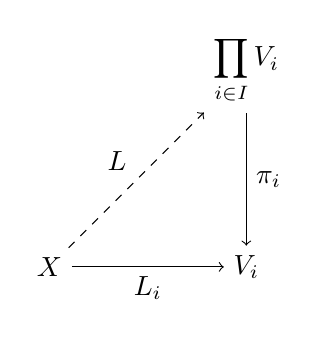
\begin{tikzpicture}[node distance=2.5cm, auto]
	\node (P) {$\displaystyle\prod_{i \in I} \bm{V_i}$};
	\node (Ci) [below of=P] {$\bm{V_i}$};
	\node (X) [left of=Ci] {$\bm X$};
	\draw[->] (X) to node [swap] {$L_i$} (Ci);
	\draw[->, dashed] (X) to node {$L$} (P);
	\draw[->] (P) to node {$\pi_i$} (Ci);
\end{tikzpicture}
\end{figure}
\end{proposition}
\begin{proof}
Defina a função
	\begin{align*}
	\func{L}{X}{\prod_{i \in I} V_i}{x}{(L_i(x))_{i \in I}}.
	\end{align*}
Da propriedade universal para conjuntos, $L$ é a única função de $X$ para $\bigtimes_{i \in I} \bm{V_i}$ tal que, para todo $i \in I$, $\pi_i \circ L = L_i$. Falta mostrar que $L$ é função linear. Sejam $c \in C$ e $x_1,x_2 \in V$. Então
	\begin{align*}
	L(x_1+cx_2) &= (L_i(x_1+cx_2))_{i \in I} \\
		&= (L_i(x_1)+cL_i(x_2))_{i \in I} \\
		&= (L_i(x_1))_{i \in I}+c(L_i(x_2))_{i \in I} \\
		&= L(x_1)+cL(x_2). \qedhere
	\end{align*}
\end{proof}

\subsection{Coproduto (soma)}

\begin{definition}
Seja $(\bm{V_i})_{i \in I} = ((V_i,+_i,\cdot_i))_{i \in I}$ uma família de espaços vetoriais. A \emph{soma categórica} de $(\bm{V_i})_{i \in I}$ é
	\begin{equation*}
	\coprod_{i \in I} \bm{V_i} = (V,+,\cdot),
	\end{equation*}
em que
	\begin{equation*}
	V = \set{v=(v_i)_{i \in I} \in \prod_{i \in I} V_i}{\card{\supp(v)} < \card{\N}},
	\end{equation*}
	\begin{align*}
	\func{+}{V \times V}{V}{(v,v')}{(v_i +_i {v'}_i)_{i \in I}}
	\end{align*}
e
	\begin{align*}
	\func{\cdot}{C \times V}{V}{(c,v)}{(cv_i)_{i \in I}.}
	\end{align*}
\end{definition}

Observe que, se $\card{I} < \card{\N}$, então $\prod_{i \in I} \bm{V_i} = \coprod_{i \in I} \bm{V_i}$.

\begin{proposition}[Propriedade Universal]
Sejam $(\bm{V_i})_{i \in I}$ uma família de espaços vetoriais sobre um corpo $\bm C$, $\bm X$ um espaço vetorial sobre $\bm C$ e, para todo $i \in I$, $L_i: \bm{V_i} \to \bm X$ uma função linear. Então existe única função linear $L: \bm X \to \coprod_{i \in I} \bm{V_i}$ tal que, para todo $i \in I$, $L \circ \iota_i = L_i$ (o diagrama comuta).
\begin{figure}
\centering
\begin{tikzpicture}[node distance=2.5cm, auto]
	\node (Ci) {$\bm{V_i}$};
	\node (S) [below of=Ci] {$\displaystyle\coprod_{i \in I} \bm{V_i}$};
	\node (X) [right of=Ci] {$\bm X$};
	\draw[->] (Ci) to node {$L_i$} (X);
	\draw[->, dashed] (S) to node [swap] {$L$} (X);
	\draw[->] (Ci) to node [swap] {$\iota_i$} (S);
\end{tikzpicture}
\end{figure}
\end{proposition}

O coproduto de espaços vetoriais é também chamado de \emph{soma} ou \emph{soma direta} e denotado
	\begin{equation*}
	\bigoplus_{i \in I} \bm{V_i}.
	\end{equation*}

%\cleardoublepage
%\section{Notas de Espaços Vetoriais Complexos}

%$(\C^m,i)$, sendo $i \cdot z:= (\sqrt{-1}z_1,\dots,\sqrt{-1}z_m)$.

%\begin{definition}
%Uma \emph{estrutura complexa} em $\R^{2m}$ é um mapa linear $j: \R^{2m} \to \R^{2m}$ que satisfaz
%	\begin{equation*}
%	j \circ j (v) = -v.
%	\end{equation*}
%\end{definition}
%
%Vamos definir uma ação de $\C$ em $\R^{2m}$.
%	\begin{equation*}
%	p(a+\sqrt{-1}b)(v) = av+bj(v).
%	\end{equation*}
%
%\begin{proposition}
%$(\R^{2m},j) \simeq (\C^m,i)$.
%\end{proposition}
%
%Para cada produto interno, temos um ângulo reto, logo uma multiplicação por $j$ distinta.
%
%Pode-se definir a partir de um vetor normal $n_p$ a um plano tangente em $p$ um mapa linear
%	\begin{equation*}
%	j_p(v) := v \times n_p
%	\end{equation*}
%que satisfaz ${j_p}^2 (v) = -v$.




\section{Projeções lineares}

\begin{definition}
Seja $\bm V$ um espaço linear sobre um corpo $\bm C$. Uma \emph{projeção linear} em $\bm V$ é uma função linear $p\colon V \to V$ idempotente: $p^2=p$.
\end{definition}

\begin{proposition}
Sejam $\bm V$ um espaço linear sobre um corpo $\bm C$ e $p\colon V \to V$ uma projeção linear.
	\begin{enumerate}
	\item $p|_{p(V)} = \Id|_{p(V)}$;
	
	\item $(\Id-p) \colon V \to V$ é uma projeção linear em $\bm V$;
	
	\item $(\Id-p)\inv(0) = p(V)$ e $(\Id-p)(V) = p\inv(0)$;
	
	\item $V = p(V) \oplus p\inv(0) = p(V) \oplus (\Id-p)(V)$;
	
	\item Para todo $\lambda \in C \setminus \{0,1\}$,
		\begin{equation*}
		(\lambda\Id-p)\inv = \frac{1}{\lambda}\Id + \frac{1}{\lambda(1-\lambda)}p
		\end{equation*}
portanto $\Esp(p) \subseteq \{0,1\}$;

	\item $p$ é invertível se, e somente se, $p=\Id$.

	\item Se $p \neq 0$, seu polinômio mínimo é $x^2-x = x(x-1)$, logo $p$ é diagonalizável pois tem raízes distintas.
	\end{enumerate}
\end{proposition}
\begin{proof}
	\begin{enumerate}	
	\item Seja $v \in p(V)$. Então existe $v' \in V$ tal que $v=p(v')$, logo
		\begin{equation*}
		p(v) = p(p(v')) = p^2(v') = p(v') = v.
		\end{equation*}
	
	\item A função $\Id-p$ é linear pois é uma diferença de funções lineares. Basta mostrar que ela é idempotente. Basta notar que% Para todo $v \in V$,
%		\begin{align*}
%		(\Id-p)^2(v) &= (\Id-p)(v-p(v)) \\
%			&= \Id(v-p(v)) - p(v-p(v)) \\
%			&= v-p(v)-p(v)+p^2(v) \\
%			&= v-p(v)-p(v)+p(v)\\
%			&= v-p(v)\\
%			&= (\Id-p)(v)
%		\end{align*}
%o que implica que $(\Id-p)^2 = \Id-p$.
		\begin{equation*}
		(\Id-p)^2 = \Id-p-p+p^2 = \Id-p-p+p = \Id-p.
		\end{equation*}
% INTERESSANTE poder multiplicar funções lineares assim, como se fosse a distributividade de multiplicação e adição. Provar isso generalizando depois.
	
	\item Seja $v \in (\Id-p)\inv(0)$. Então $(\Id-p)(v)=0$, logo $v=p(v)$, o que implica que $v \in p(V)$. Reciprocamente, seja $v \in p(V)$. Então do item 1 segue que $p(v) = v$, logo $(\Id-p)(v) = v-p(v) = v-v = 0$.

A outra relação segue de $(\Id-p)$ ser projeção e $p = \Id - (\Id-p)$.

	\item Seja $v \in p(V) \cap p\inv(0)$. Então $p(v)=0$ e $p(v)=v$, o que implica que $v = p(v) = 0$. Assim temos que $p(V) \cap p\inv(0) = \{0\}$.
%Sejam $v in p(V)$ e $v' \in p\inv(0)$ e $c,c' \in C$ tais que $cv+c'v'=0$. Então
%		\begin{equation*}
%		0 = p(0) = p(cv+c'v') = cp(v)+c'p(v') = cv
%		\end{equation*}
%logo $c=0$, portanto $0 = cv+c'v'=c'v'$, o que implica que $c'=0$.
	
	Seja $v \in V$. Então $p(v) \in p(V)$ e $(\Id-p)(v) \in p\inv(0)$ (pois $(\Id-p)(V) = p\inv(0)$), logo $v = p(v) + (\Id-p)(v)$, o que mostra que $V = p(V) + p\inv(V)$.
	
	\item Note que
		\begin{equation*}
		\frac{1}{1-\lambda} - \frac{1}{\lambda} - \frac{1}{\lambda(1-\lambda)} = \frac{\lambda - (\lambda - 1) - 1}{\lambda(1-\lambda)} = 0,
		\end{equation*}
logo
		\begin{align*}
		(\lambda\Id - p) \circ \left( \frac{1}{\lambda}\Id + \frac{1}{\lambda(1-\lambda)}p \right) &= \Id + \frac{1}{1-\lambda}p - \frac{1}{\lambda}p - \frac{1}{\lambda(1-\lambda)}p^2 \\
%			&= \Id + \frac{1}{1-\lambda}p - \frac{1}{\lambda}p - \frac{1}{\lambda(1-\lambda)}p \\
			&= \Id + \left( \frac{1}{1-\lambda} - \frac{1}{\lambda} - \frac{1}{\lambda(1-\lambda)} \right) p \\
			&= \Id.
		\end{align*}
e
	\begin{equation*}
	\left( \frac{1}{\lambda}\Id + \frac{1}{\lambda(1-\lambda)}p \right) \circ (\lambda\Id - p) = \Id - \frac{1}{\lambda}p + \frac{1}{1-\lambda}p - \frac{1}{\lambda(1-\lambda)}p^2 = \Id.
	\end{equation*}
	
	\item Se $p$ é invertível, $V=p(V)$, logo
		\begin{equation*}
		p = p|_{V} = p|_{p(V)} = \Id|_{p(V)} = \Id|_V = \Id.
		\end{equation*}
A recíproca é evidente.

	\item Evidente.
	
	\end{enumerate}
\end{proof}




%\chapter{Álgebra Multilinear}

\section{Funções multilineares}

\begin{definition}
Sejam $\bm{V_0},\cdots,\bm{V_{k-1}}$ e $\bm W$ espaços lineares sobre um corpo $\bm C$ e $k \in \N$. Uma função \emph{$k$-linear} de $(\bm{V_0},\ldots,\bm{V_{k-1}})$ para $\bm W$ é uma função
	\begin{equation*}
	L\colon V_0 \times \cdots \times V_{k-1} \to W
	\end{equation*}
qua satisfaz
	\begin{enumerate}
	\item (Multilinearidade) Para todos $i \in [k]$ e
	\begin{equation*}
	(v_0,\ldots,v_{i-1},v_{i+1},\ldots,v_{k-1}) \in V_0 \times \cdots \times V_{i-1} \times V_{i+1} \times \cdots \times V_{k-1},
	\end{equation*}
a função
	\begin{align*}
	\func{L(v_0,\ldots,v_{i-1},\var,v_{i+1},\ldots,v_{k-1})}{\bm{V_i}}{\bm W}{v}{L(v_0,\ldots,v_{i-1},v,v_{i+1},\ldots,v_{k-1})}
	\end{align*}
%	\begin{align*}
%	\func{L(\bm v_0,\ldots,\underbrace{\var}_i,\ldots,\bm v_{k-1})}{\bm{V_i}}{\bm W}{\bm v}{L(\bm v_0,\ldots,\underbrace{\bm v}_i,\ldots,\bm v_{k-1})}
%	\end{align*}
é uma função linear.
	\end{enumerate}
O conjunto dessas funções é denotado
	\begin{equation*}
	\lin(V_0,\ldots,V_{k-1};W)
	\end{equation*}
e, quando todos os espaços $\bm{V_i}$ são iguais, denota-se
	\begin{equation*}
	\lin^k(V,W) := \lin(\underbrace{V,\ldots,V}_k;W)
	\end{equation*}
\end{definition}

\begin{proposition}
Sejam $\bm{V_0},\cdots,\bm{V_{k-1}}$ e $\bm W$ espaços lineares sobre um corpo $\bm C$ e, para cada $i \in [k]$, $d_i \in \N$ a dimensão e $b^{(i)}=(b^{(i)}_j)_{j \in [d_i]}$ uma base ordenada de $\bm{V_i}$. Toda função $k$-linear $L \in \lin(V_0,\ldots,V_{k-1};W)$ está determinada pelos seus valores em $(b^{(0)}_{j_0},\ldots,b^{(k-1)}_{j_{k-1}})_{(j_0,\ldots,j_{k-1}) \in [d_0] \times \cdots \times [d_{k-1}]}$.
\end{proposition}
\begin{proof}
Sejam $v_0,\ldots,v_{m-1} \in V_k$, $c^0,\ldots,c^{m-1} \in C$, e, para todo $i \in [k]\setminus \{k\}$, $v'_i \in V_i$. Como consequência da propriedade de linearidade generalizada para funções lineares,
	\begin{equation*}
	L\left(v'_0,\ldots,\sum_{i \in [m]} c^i v_i,\ldots,v'_{k-1} \right) = \sum_{i \in [m]} c^i L\left(v'_0,\ldots,v_i,\ldots,v'_{k-1} \right).
	\end{equation*}
Sendo assim, para cada $i \in [k]$, sejam $v_i \in V_i$ e $v_{(i)}^0,\ldots,v_{(i)}^{d_i} \in C$ os coeficientes de $v_i$ na base $b^{(i)}$, de modo que
	\begin{equation*}
	v_i = \sum_{j \in [d_i]} v_{(i)}^j b^{(i)}_j.
	\end{equation*}
Pela linearidade em cada entrada, temos que
	\begin{align*}
	L(v_0,\ldots,v_{k-1}) &= L\left(\sum_{j_0 \in [d_0]} v_{(0)}^{j_0}b^{(0)}_{j_0},\ldots,\sum_{j_{k-1} \in [d_{k-1}]} v_{(k-1)}^{j_{k-1}} b^{(k-1)}_{j_{k-1}} \right) \\
		&= \sum_{j_0 \in [d_0]} v_{(0)}^{j_0} L\left(b^{(0)}_{j_0},\ldots,\sum_{j_{k-1} \in [d_{k-1}]} v_{(k-1)}^{j_{k-1}} b^{(k-1)}_{j_{k-1}} \right) \\
		&\ \, \vdots\qquad\qquad\qquad\qquad\qquad \vdots \\
		&= \sum_{j_0 \in [d_0]} \cdots \sum_{j_{k-1} \in [d_{k-1}]} v_{(0)}^{j_0} \cdots v_{(k-1)}^{j_{k-1}} L\left(b^{(0)}_{j_0},\ldots,b^{(k-1)}_{j_{k-1}} \right) \\
		&= \sum_{(j_0,\ldots,j_{k-1}) \in [d_0] \times \cdots \times [d_{k-1}]} v_{(0)}^{j_0} \cdots v_{(k-1)}^{j_{k-1}} L\left(b^{(0)}_{j_0},\ldots,b^{(k-1)}_{j_{k-1}} \right).
	\end{align*}
%			&= \sum_{\substack{j_0 \in [d_0] \\ \cdots\\ j_{k-1} \in [d_{k-1}]}} v_{0,j_0} \cdots v_{k-1,j_{k-1}} L\left(b_{0,j_0},\ldots,b_{k-1,j_{k-1}} \right).
Portanto a função $L$ está determinada pelos valores que tem nos elementos
	\begin{equation*}
	(b^{(0)}_{j_0},\ldots,b^{(k-1)}_{j_{k-1}})_{(j_0,\ldots,j_{k-1}) \in [d_0] \times \cdots \times [d_{k-1}]}.
	\end{equation*}
%Como há $d_0 \cdots d_{k-1}$ desses elementos, há essa quantidade de escolhas a serem determinadas para se determinarem os valores de $L$.
\end{proof}

\begin{proposition}
Sejam $\bm{V_0},\cdots,\bm{V_{k-1}}$ e $\bm W$ espaços lineares sobre um corpo $\bm C$. Então
	\begin{equation*}
	\lin(\bm{V_0},\ldots,\bm{V_{k-1}};\bm W) := (\lin(V_0,\ldots,V_{k-1};W),+,\cdot),
	\end{equation*}	
em que $+$ e $\cdot$ são a soma e o produto escalar pontuais induzidos por $\bm W$, é um espaço linear sobre $\bm C$.
\end{proposition}

%Mostrar isomorfismo
%	\begin{align*}
%	\func{\Omega}{\lin^2(V_0,V_1;W)}{\lin(V_0,\lin(V_1,W))}{L}{L(v_0,\var)}.
%	\end{align*}

\subsection{Simetria, antissimetria e alternância}

\begin{definition}
Sejam $\bm V$ e $\bm W$ espaços lineares sobre um corpo $\bm C$. Uma função $k$-linear de $\bm V$ para $\bm W$
\begin{enumerate}
	\item \emph{simétrica} é uma função $f \in \lin^k(\bm V,\bm W)$ tal que, para toda permutação $p \in \sime_k$ e todos $v_0$, $\ldots$, $v_{k-1} \in V$,
	\begin{equation*}
	f(v_{p(0)},\ldots,v_{p(k-1)}) = f(v_0,\ldots,v_{k-1});
	\end{equation*}
O conjunto das funções $k$-lineares simétricas é denotado $\mathcal S^k(\bm V,\bm W)$.
	\item \emph{antissimétrica} é uma função $f \in \lin^k(\bm V,\bm W)$ tal que, para toda permutação $p \in \sime_k$ e todos $v_0,\ldots,v_{k-1} \in V$,
	\begin{equation*}
	f(v_{p(0)},\ldots,v_{p(k-1)}) = \prd(p) f(v_0,\ldots,v_{k-1});
	\end{equation*}
	\item \emph{alternada} é uma função $f \in \lin^k(\bm V,\bm W)$ tal que, para todos $v_0,\ldots,v_{k-1} \in V$ linearmente dependentes,
	\begin{equation*}
	f(v_0,\ldots,v_{k-1}) = 0.
	\end{equation*}
O conjunto das funções $k$-lineares alternadas é denotado $\mathcal A^k(\bm V,\bm W)$.
\end{enumerate}
\end{definition}

\begin{proposition}
Sejam $\bm V$ e $\bm W$ espaços lineares sobre um corpo $\bm C$ e $f \in \lin^k(\bm V,\bm W)$.
	\begin{enumerate}
	\item A função $f$ é alternada se, e somente se, para todos $v_0$, $\ldots$, $v_{k-1} \in V$ tais que existem $i,j \in [k]$ distintos satisfazendo $v_i = v_j$,
	\begin{equation*}
	f(v_0,\ldots,v_{k-1})=0.
	\end{equation*} 
	\item Se $f$ é alternada, então é antissimétrica. Se $\car(\bm C) \neq 2$ e $f$ é antissimétrica, então é alternada.
	\item Se $\car(\bm C) = 2$, então $f$ é antissimétrica se, e somente se, é simétrica.
	\end{enumerate}
\end{proposition}
\begin{proof}
	\begin{enumerate}
	\item Se $f$ é alternada, então, para todos $v_0,\ldots,v_{k-1} \in V$ tais que $v_i = v_j$ para dois $i,j \in [k]$ distintos, o conjunto $\{v_0,\ldots,v_{k-1}\}$ é linearmente dependente, portanto $f(v_0,\ldots,v_{k-1})=0$. Reciprocamente, suponha que $f$ satisfaz a propriedade e sejam $v_0,\ldots,v_{k-1} \in V$ linearmente dependentes. Então existe $i \in [k]$ tal que $v_i$ é combinação linear dos outros $v_j$: existem $c_j \in C$, com $j \in [k]\setminus\{i\}$, tais que
	\begin{equation*}
	v_i = \sum_{j \in [k]\setminus\{i\}} c_j v_j.
	\end{equation*}
Assim, segue da $k$-linearidade e da propriedade enunciada que
	\begin{align*}
	f(v_0,\ldots,v_{k-1}) &= f\left(v_0,\ldots, \sum_{j \in [k]\setminus\{i\}} c_j v_j,\ldots,v_{k-1}\right) \\
		&= \sum_{j \in [k]\setminus\{i\}} c_j f(v_0,\ldots,v_j,\ldots,v_{k-1}) \\
		&=\sum_{j \in [k]\setminus\{i\}} c_j 0 = 0.
	\end{align*}

	\item Suponha $f$ alternada e sejam $v_0,\ldots,v_{k-1} \in V$. Então segue da $k$-linearidade e da alternância de $f$ que
	\begin{align*}
	0 =&f(v_0,\ldots,v_i+v_j,\ldots,v_i+v_j,\ldots,v_{k-1}) \\
		=& f(v_0,\ldots,v_i,\ldots,v_i,\ldots,v_{k-1}) + f(v_0,\ldots,v_i,\ldots,v_j,\ldots,v_{k-1}) \\
		&+f(v_0,\ldots,v_j,\ldots,v_i,\ldots,v_{k-1}) + f(v_0,\ldots,v_j,\ldots,v_j,\ldots,v_{k-1}) \\
		=& f(v_0,\ldots,v_i,\ldots,v_j,\ldots,v_{k-1}) +f(v_0,\ldots,v_j,\ldots,v_i,\ldots,v_{k-1}),
	\end{align*}
portanto
	\begin{equation*}
	f(v_0,\ldots,v_i,\ldots,v_j,\ldots,v_{k-1}) = - f(v_0,\ldots,v_j,\ldots,v_i,\ldots,v_{k-1}).
	\end{equation*}
Como toda permutação $p \in \sime_k$ é um produto de $N \in \N$ inversões, e como $\prd(p)=(-1)^N$, segue por indução que, para toda permutação $p \in \sime_k$,
	\begin{equation*}
	f(v_{p(0)},\ldots,v_{p(k-1)}) =(-1)^N f(v_0,\ldots,v_{k-1}) = \prd(p) f(v_0,\ldots,v_{k-1}).
	\end{equation*}

Suponha que $\car(\bm C) \neq 2$. Sejam $f \in \lin^k(\bm V,\bm W)$ antissimétrica e $v_0$, $\ldots$, $v_{k-1} \in V$ tais que $v_i = v_j$ para dois $i,j \in [k]$ distintos. Considerando a permutação $(i \quad j) \in \sime_k$, segue da antissimetria de $f$ e de $\prd((i \quad j))=-1$ que
	\begin{align*}
	f(v_0,\ldots,v_i,\ldots,v_j,\ldots,v_{k-1}) &= f(v_0,\ldots,v_j,\ldots,v_i,\ldots,v_{k-1}) \\
		&= - f(v_0,\ldots,v_i,\ldots,v_j,\ldots,v_{k-1}),
	\end{align*}
portanto
	\begin{equation*}
	2 f(v_0,\ldots,v_{k-1})=0.
	\end{equation*}
Como $\car(\bm C) \neq 2$, segue que $f(v_0,\ldots,v_{k-1})=0$. Do item 1 segue que $f$ é alternada.

\item Se $\car(\bm C) = 2$, então $-1=1$. Isso implica que, para qualquer permutação $p$, $\prd(p)=1$.
\end{enumerate}
\end{proof}

Um exemplo de uma função multilinear que é antissimétrica mas não é alternada em para um corpo de característica $2$ é o seguinte. Seja $\Z_2=\{0,1\}$ o corpo de característica $2$ e considere a função $f\colon \Z_2 \times \Z_2 \to \Z_2$ dada por
	\begin{align*}
	\func{f}{\Z_2 \times \Z_2}{\Z_2}{(0,0)}{0 \\
															(0,1) &\mapsto 0 \\
															(1,0) &\mapsto 0 \\
															(1,1) &\mapsto 1												
														}
	\end{align*}
Pode-se verificar que essa função é bilinear e antissimétrica, mas não é alternada porque $f(1,1)=1 \neq 0$.

De modo mais geral, para qualquer função $p\colon [k] \to [k]$, não necessariamente bijetiva, considerando o caráter $\prd(p)$ que vale $0$ se $p$ não é uma permutação, e $1$ ou $-1$ conforme a paridade da permutação $p$, as definições de formas antissimétricas e alternadas podem ser unificadas: a de formas antissimétricas pode ser mantida como foi feita e, para o caso de formas alternadas, devido à propriedade 1 da proposição anterior, pode-se enunciar: para qualquer $p\colon [k] \to [k]$,
	\begin{equation*}
	f(v_{p(0)},\ldots,v_{v_{k-1}}) = \prd(p) f(v_0,\ldots,v_{k-1}).
	\end{equation*}
O caso em que $p$ é bijetiva recai na definição de formas antissimétricas, e o caso em que $p$ não é bijetiva recai na definição de formas alternadas, mais precisamente da propriedade 1 da proposição anterior, que é equivalente à definição de forma alternada.

\begin{proposition}
Sejam $\bm V$ e $\bm W$ espaços lineares sobre um corpo $\bm C$. Os espaços $\mathcal S^k(\bm V,\bm W)$ e $\mathcal A^k(\bm V,\bm W)$ são subespaços lineares de $\lin^k(\bm V,\bm W)$.
\end{proposition}

\section{Formas multilineares}

\begin{definition}
Seja $\bm V$ um espaço linear sobre um corpo $\bm C$. Uma \emph{forma $k$-linear} em $\bm V$ é uma função $f \in \lin^k(\bm V;\bm C)$, ou seja, um funcional $k$-linear em $(\bm V,\ldots,\bm V)$. O conjunto das formas $k$-lineares simétricas é denotado $\mathcal{S}^k(\bm V)$ e o das alternadas é denotado $\mathcal{A}^k(\bm V)$.
\end{definition}

Temos que $\mathcal{S}^1(\bm V) = \mathcal{A}^1(\bm V) = \lin^k(\bm V)$ e $\mathcal{S}^0(\bm V) = \mathcal{A}^0(\bm V) = \lin^0(\bm V) = C$.

\subsection{Produto tensorial de formas multilineares}

\begin{definition}
Sejam $\bm V$ um espaço linear sobre um corpo $\bm C$, $f \in \lin^k(V)$, $f' \in \lin^{k'}(V)$ e $v_0,\ldots,v_{k+k'-1} \in V$. O \emph{produto tensorial} de $f$ e $f'$ em $(v_0,\ldots,v_{k+k'-1})$ é
	\begin{equation*}
	(f \otimes f')(v_0,\ldots,v_{k+k'-1}) := f(v_0,\ldots,v_{k-1})f'(v_k,\ldots,v_{k+k'-1}).
	\end{equation*}
Sejam $n \in \N$ e $(f_i)_{i \in [n]}$ formas multilineares em $\bm V$. O \emph{produto tensorial} dessas formas é definido recursivamente
	\begin{equation*}
	\bigotimes_{i \in [n]} f_i := \begin{cases}
		f_0,& n=1 \\
		\left(\displaystyle\bigotimes_{i \in [n-1]} f_i \right) \otimes f_{n-1} ,& n>1.
	\end{cases}
	\end{equation*}
\end{definition}

\begin{proposition}
Seja $\bm V$ um espaço linear sobre um corpo $\bm C$.
	\begin{enumerate}
	\item Para todas formas $f \in \lin^k(\bm V)$ e $f' \in \lin^{k'}(\bm V)$, a função $f \otimes f'$ é uma forma $k+k'$-linear.
	\item (Bilinearidade) A função
		\begin{align*}
		\func{\otimes}{\lin^k(\bm V) \times \lin^{k'}(\bm V)}{\lin^{k+k'}(\bm V)}{(f,f')}{f \otimes f'}
		\end{align*}
é bilinear.
	\item (Associatividade) Para todas formas $f \in \lin^k(\bm V)$, $f' \in \lin^{k'}(\bm V)$ e $f'' \in \lin^{k''}(\bm V)$,
		\begin{equation*}
		(f \otimes f') \otimes f'' = f \otimes (f' \otimes f'').
		\end{equation*}
	\end{enumerate}
\end{proposition}

\subsection{Produto alternado de formas multilineares}

\begin{definition}
Sejam $\bm V$ um espaço linear sobre um corpo $\bm C$, $f \in \mathcal{A}^k(\bm V)$, $f' \in \mathcal{A}^{k'}(\bm V)$ e $v_0,\ldots,v_{k+k'-1} \in \bm V$. O \emph{produto alternado} (ou \emph{exterior}) de $f$ e $f'$ em $(v_0,\ldots,v_{k+k'-1})$ é
%	\begin{equation*}
%	(f \wedge f')(v_0,\ldots,v_{k+k'-1}) := \frac{1}{k!k'!} \sum_{p \in \sime_{k+k'}} \prd(p) f(v_{p(0)},\ldots,v_{p(k-1)})f'(v_{p(k)},\ldots,v_{p(k+k'-1)}).
%	\end{equation*}
	\begin{equation*}
	(f \wedge f')(v_0,\ldots,v_{k+k'-1}) := \frac{1}{k!k'!} \sum_{p \in \sime_{k+k'}} \prd(p) (f \otimes f')(v_{p(i)})_{i \in [k+k']}.
	\end{equation*}
Sejam $n \in \N$ e $(f_i)_{i \in [n]}$ formas multilineares em $\bm V$. O \emph{produto alternado} dessas formas é definido recursivamente
	\begin{equation*}
	\bigwedge_{i \in [n]} f_i := \begin{cases}
		f_0,& n=1 \\
		\left(\displaystyle\bigwedge_{i \in [n-1]} f_i \right) \wedge f_{n-1} ,& n>1.
	\end{cases}
	\end{equation*}
\end{definition}

\begin{proposition}
Seja $\bm V$ um espaço linear sobre um corpo $\bm C$.
	\begin{enumerate}
	\item Para todas formas $f \in \lin^k(\bm V)$ e $f' \in \lin^{k'}(\bm V)$, a função $f \wedge f'$ é uma forma $k+k'$-linear alternada.
	\item (Bilinearidade) A função
		\begin{align*}
		\func{\wedge}{\mathcal{A}^k(\bm V) \times \mathcal{A}^{k'}(\bm V)}{\mathcal{A}^{k+k'}(\bm V)}{(f,f')}{f \wedge f'}
		\end{align*}
é bilinear.
	\item (Associatividade) Para todas formas alternadas $f \in \mathcal{A}^k(\bm V)$, $f' \in \mathcal{A}^{k'}(\bm V)$ e $f'' \in \mathcal{A}^{k''}(\bm V)$,
		\begin{equation*}
		(f \wedge f') \wedge f'' = f \wedge (f' \wedge f'').
		\end{equation*}
	\item	 Para todas formas $f \in \mathcal{A}^k(\bm V)$ e $f' \in \mathcal{A}^{k'}(\bm V)$
		\begin{equation*}
		f' \wedge f = (-1)^{kk'} f \wedge f'.
		\end{equation*}
	\end{enumerate}
\end{proposition}
\begin{proof}
	\begin{enumerate}
	\item Seja $v_0,\ldots,v_{k+k'-1} \in V$ e $\bar p \in \sime_{k+k'}$. Então
		\begin{align*}
		(f \wedge f') (v_{\bar p(i)})_{i \in [k+k']} &= \frac{1}{k!k'!} \sum_{p \in \sime_{k+k'}} \prd(p) (f \otimes f')(v_{p(\bar p(i))})_{i \in [k+k']} \\
			&= \frac{1}{k!k'!} \sum_{p \in \sime_{k+k'}} \prd(\bar p\inv p) (f \otimes f')(v_{p(i)})_{i \in [k+k']} \\
			&= \frac{1}{k!k'!} \sum_{p \in \sime_{k+k'}} \prd(\bar p\inv)\prd(p) (f \otimes f')(v_{p(i)})_{i \in [k+k']} \\
			&= \prd(\bar p\inv)\frac{1}{k!k'!} \sum_{p \in \sime_{k+k'}} \prd(p) (f \otimes f')(v_{p(i)})_{i \in [k+k']} \\
			&= \prd(\bar p)(f \wedge f')(v_i)_{i \in [k+k']}.
		\end{align*}
	\item	 
	\end{enumerate}
\end{proof}

%Isso define uma função bilinear
%	\begin{align*}
%	\func{\wedge}{\mathcal{A}^k(\bm V) \times \mathcal{A}^l(\bm V)}{\mathcal{A}^{k+l}(\bm V)}{(f,g)}{f \wedge g}
%	\end{align*}

%Esse produto é uma forma $\sum_{i \in [n]} k_i$-linear em $\bm V$.

%\begin{definition}
%Sejam $\bm V$ um espaço linear de dimensão finita $d$ sobre um corpo $\bm C$, $(b_i)_{i \in [d]}$ um base ordenada de $\bm V$ e $({b_i}^*)_{i \in [d]}$ a base dual de $\bm{V^*}$. Para todo subconjunto $I \subseteq [d]$, e $(i_j)_{j \in [\card{I}]}$ a indexação crescente de $I$ ($i_0 < \cdots < i_{\card{I}-1}$), define-se
%	\begin{equation*}
%	\bigwedge_{i \in I} b_i^* := b_{i_0}^* \wedge \cdots \wedge b_{i_{k-1}}^*.
%	\end{equation*}
%\end{definition}

\begin{proposition}
Sejam $\bm V$ um espaço linear de dimensão finita $d$ sobre um corpo $\bm C$, $(b_i)_{i \in [d]}$ um base ordenada de $\bm V$ e $({b_i}^*)_{i \in [d]}$ a base dual de $\bm{V^*}$. Então $\mathcal{A}^k(\bm V)$ é um espaço linear sobre $\bm C$ de dimensão $\binom{d}{k}$ e o conjunto
	\begin{equation*}
	\set{b_{i_0}^* \wedge \cdots \wedge b_{i_{k-1}}^*}{i_0 < \cdots < i_{k-1} \in [d]}
	\end{equation*}
%	\begin{equation*}
%	\set{\bigwedge_{i \in I} b_{i}^*}{I \subseteq [d], \card{I}=k}
%	\end{equation*}
de formas alternadas $k$-lineares em $\bm V$ é uma base para $\mathcal{A}^k(\bm V)$.
\end{proposition}

Em particular, isso mostra que formas $d$-lineares num espaço de dimensão $d$ são todas múltiplos umas das outras, pois $\binom{d}{d}=1$. Podemos fixar o valor de uma das formas como 1 na base canônica e chamá-la de \emph{determinante}.

\begin{definition}
Seja $d \in \N$. O \emph{determinante} em $\R^d$ é a forma $d$-linear
	\begin{equation*}
	\det := {\ii_0}\dual \wedge \ldots \wedge {\ii_{d-1}}\dual.
	\end{equation*}
%Sejam $\bm V$ um espaço linear de dimensão finita $d$ sobre um corpo $\bm C$ e $b=(b_i)_{i \in [d]}$ uma base de $\bm V$. O \emph{determinante} em $\bm V$ com respeito a $b$ é a forma $d$-linear
%	\begin{equation*}
%	\det\nolimits_{b} := {b_0}\dual \wedge \ldots \wedge {b_{d-1}}\dual.
%	\end{equation*}
%No caso de $V = \R^d$, o determinante é definido com respeito à base canônica
%	\begin{equation*}
%	\det := {\ii_0}\dual \wedge \ldots \wedge {\ii_{d-1}}\dual.
%	\end{equation*}
\end{definition}

Como comentado, essa é a única forma $d$-linear em $\R^d$ tal que	\begin{equation*}
	\det(\ii_0,\ldots,\ii_{d-1})=1.
	\end{equation*}

Na seção seguinte, definiremos o conceito de determinante de modo mais geral e independente de base.

\subsection{Formas puxadas e determinante}

\begin{definition}
Sejam $\bm V$ e $\bm V'$ espaços lineares sobre um corpo $\bm C$, $L \colon V \to V'$ uma função linear e $f \in \lin^k(V')$. A \emph{forma $k$-linear puxada} por $L$ de $f$ é a função
	\begin{align*}
	\func{L\dual f}{V^k}{C}{(v_0,\ldots,v_{k-1})}{f(L(v_0),\ldots,L(v_{k-1})).}
	\end{align*}
A função \emph{$k$-adjunta} induzida por $L$ é a função linear
	\begin{align*}
	\func{L\dual}{\lin^k(V')}{\lin^k(V)}{f}{L\dual f.}
	\end{align*}
\end{definition}

A notação é ambígua porque, para cada $k \in [d+1]$, a função $L\dual$ é uma função diferente. De fato, para $f \in \lin^k(V')$,
	\begin{equation*}
	L\dual f = f \circ L^{\otimes k},
	\end{equation*}
o que quer dizer que
	\begin{equation*}
	L \dual = (L^{\otimes k})\pux
	\end{equation*}

\begin{proposition}
Sejam $\bm V$, $\bm V'$ e $\bm V''$ espaços lineares sobre um corpo $\bm C$ e $L\colon V \to V'$ e $L'\colon V' \to V''$ funções lineares. Então
	\begin{equation*}
	(L' \circ L)\dual = {L}\dual \circ {L'}\dual.
	\end{equation*}
\end{proposition}
\begin{proof} Seja $f \in \lin^k(V)$ tal que $f \neq 0$. Então
	\begin{align*}
	(L' \circ L)\dual f (v_0,\ldots,v_{k-1}) &= f((L' \circ L)(v_0),\ldots,(L' \circ L)(v_{k-1})) \\
		&= f(L'(L(v_0)),\ldots,L'(L(v_{k-1}))) \\
		&= {L'}\dual f(L(v_0),\ldots,L(v_{k-1})) \\
		&= L\dual({L'}\dual f)(v_0,\ldots,v_{k-1}) \\
		&= (L\dual \circ {L'}\dual) f(v_0,\ldots,v_{k-1}).
	\end{align*}
\end{proof}


Essas funções $k$-adjuntas estão também definidas se restringimos os espaços de funcionais $\lin^k$ para espaços de funcionais alternados $\alter^k$. Se considerarmos um espaço linear $d$-dimensional $\bm V$, o espaço $\alter^d(\bm V)$ é um espaço $1$-dimensional, o que implica que todas funções lineares são multiplicações por constantes. Isso nos permite definir o determinante de uma função linear intrinsecamente como a constante de é seu $d$-adjunto.

\begin{definition}
Sejam $\bm V$ um espaço linear $d$-dimensional sobre um um corpo $\bm C$, $L\colon V \to V$ uma função linear e $L\dual\colon \alter^d(V) \to \alter^d(V)$. O \emph{determinante} de $L$ é a constante $\det(L) \in C$ tal que, para todas formas $f \in \alter^d(\bm V)$,
	\begin{equation*}
	L\dual f = \det(L) f.
	\end{equation*}
\end{definition}

Isso nos dá por definição a igualdade
	\begin{equation*}
	f(L(v_0),\ldots,L(v_{d-1})) = \det(L)f(v_0,\ldots,v_{d-1}).
	\end{equation*}

\begin{proposition}
Sejam $\bm V$ um espaço linear $d$-dimensional sobre um um corpo $\bm C$ e $L,L' \in \lin(V,V)$. Então
	\begin{equation*}
	\det(L' \circ L) = \det(L)\det(L').
	\end{equation*}
\end{proposition}
\begin{proof}
Seja $f \in \alter^n(V)$ tal que $f \neq 0$. Então
	\begin{equation*}
	\det(L' \circ L)f = (L' \circ L)\dual f = ({L}\dual \circ {L'}\dual) f = \det(L)\det(L') f.
	\end{equation*}
\end{proof}

\begin{proposition}
Sejam $\bm V$ um espaço linear $d$-dimensional sobre um um corpo $\bm C$ e $L\colon V \to V$ uma função linear. Então $L$ é invertível se, e somente se, $\det(L) \neq 0$.
\end{proposition}
\begin{proof}
Basta notar que $L$ é invertível se, e somente se, leva base em base e $f \in \alter^d(V)$ é nula em um conjunto linearmente independente de vetores.
\end{proof}


\subsection{\ensuremath{2}-Formas reais e os espaços \ensuremath{\R^{p,q}}}

Definimos agora espaços reais munidos de formas bilineares simétricas não-degeneradas.

\begin{definition}
Sejam $p,q \in \Z_{>}$. A \emph{$2$-forma simétrica canônica de assinatura $(p,q)$} é a $2$-forma
	\begin{align*}
	\func{\inte{\var}{\var}_{p,q}}{\R^{p+q} \times \R^{p+q}}{\R}{(x,x')}{\sum_{k=0}^{p-1}{x_k}^2 - \sum_{k=p}^{p+q-1}{x_k}^2}
	\end{align*}
\end{definition}

Para ver que essa função é bilinear, basta ver que na base canônica $(\ii_k)_{k \in [p+q]}$, ela é dada por
	\begin{equation*}
	\inte{\ii_k}{\ii_{k'}}_{p,q} =
		\begin{cases}
		\delta_{k,k'}	& 0 \leq k,k' \leq p-1 \\
		-\delta_{k,k'}	& p \leq k,k' \leq p+q-1 \\
		0				& \text{c.c.}.
		\end{cases}
	\end{equation*}
e que a partir disso obtemos
	\begin{align*}
	\inte{x}{x'}_{p,q} &= \inte{\sum_{k=0}^{p-1} x_k\ii_k + \sum_{k=p}^{p+q-1} x_k\ii_k}{\sum_{k'=0}^{p-1} x_{k'}\ii_{k'} + \sum_{k'=p}^{p+q-1} x_{k'}\ii_{k'}}_{p,q} \\
		&= \inte{\sum_{k=0}^{p-1} x_k\ii_k}{\sum_{k'=0}^{p-1} x_{k'}\ii_{k'}}_{p,q} + \inte{\sum_{k=0}^{p-1} x_k\ii_k}{\sum_{k'=p}^{p+q-1} x_{k'}\ii_{k'}}_{p,q} \\
		&+ \inte{\sum_{k=p}^{p+q-1} x_k\ii_k}{\sum_{k'=0}^{p-1} x_{k'}\ii_{k'}}_{p,q} + \inte{\sum_{k=p}^{p+q-1} x_k\ii_k}{\sum_{k'=p}^{p+q-1} x_{k'}\ii_{k'}}_{p,q} \\
		&= \sum_{k=0}^{p-1} \sum_{k'=0}^{p-1} x_kx_{k'}\inte{\ii_k}{\ii_{k'}}_{p,q} + \sum_{k=0}^{p-1} \sum_{k'=p}^{p+q-1} x_k x_{k'} \inte{\ii_k}{\ii_{k'}}_{p,q} \\
		&+ \sum_{k=p}^{p+q-1} \sum_{k'=0}^{p-1} x_k x_{k'} \inte{\ii_k}{\ii_{k'}}_{p,q} + \sum_{k=p}^{p+q-1} \sum_{k'=p}^{p+q-1} x_k x_{k'} \inte{\ii_k}{\ii_{k'}}_{p,q} \\
		&= \sum_{k=0}^{p-1}{x_k}^2 - \sum_{k=p}^{p+q-1}{x_k}^2.
	\end{align*}

O espaço linear $\R^{p+q}$ dotado dessa forma é denotado $\R^{p,q}$.


\cleardoublepage





\section{Produto tensorial de espaços lineares}

\begin{definition}
Sejam $X$ um conjunto, $\bm C$ um corpo e $f: X \to C$ uma função. O \emph{suporte} de $f$ é o conjunto
	\begin{equation*}
	\supp(f) := f\inv\left(\{0\}^\complement\right) = \set{x \in X}{f(x) \neq 0}.
	\end{equation*}
\end{definition}

%\begin{definition}
%Sejam $I$ um conjunto e $\bm C$ um corpo. Uma \emph{combinação linear formal} de elementos de $I$ sobre $\bm C$ é uma função $v: I \to C$ de suporte finito. Definido $c_i := v(i) \in C$, denota-se
%	\begin{equation*}
%	v = \sum_{i \in I} c_i v_i.
%	\end{equation*}
%\end{definition}

\begin{definition} Sejam $I$ um conjunto e $\bm C$ um corpo. O \emph{espaço linear livre em $I$} sobre $\bm C$ é o conjunto 
	\begin{equation*}
	\liv(I) := \set{v \in C^I}{\card{\supp(v)}<\card{\N}}.
	\end{equation*}
Os elementos de $\liv(I)$ são as \emph{combinações lineares formais} de elementos de $I$ sobre $\bm C$.

A \emph{inclusão} de $I$ em $\liv(I)$ é a função
	\begin{align*}
	\func{\iota}{I}{\liv(I)}{v}{
		\begin{aligned}[t]
		\func{\delta_v}{I}{C}{i}{\begin{cases}
							1,& i = v \\
							0,& i \neq v.
						\end{cases}}
		\end{aligned}	
	}
	\end{align*}
Denotaremos os elementos $\delta_v$ por $v$ quando não houver necessidade de diferenciá-los.
\end{definition}

Note que $\liv(I) = \coprod_{i \in I} \bm C$ e, portanto,
	\begin{equation*}
	\bm{\liv(I)} := (\liv(I)),+,\cdot),
	\end{equation*}	
em que $+$ e $\cdot$ são a soma e o produto escalar pontuais induzidos por $\bm W$, é um espaço linear sobre $\bm C$ com base $\set{\delta_v}{v \in I}$. Por isso, definido $c_i := v(i) \in C$, uma função $v: I \to C$ de suporte finito é uma soma
	\begin{equation*}
	v = \sum_{i \in I} c_i \delta_i = \sum_{i \in I} c_i v_i,
	\end{equation*}
que é uma soma finita porque $\supp(v)$ é finito, ou seja, somente uma quantidade finita dos $c_i$ é não nulo.

\begin{proposition}[Propriedade Caracterítica dos Espaços Lineares Livres]
Sejam $I$ um conjunto, $\bm C$ um corpo e $\bm V$ um espaço linear sobre $\bm C$. Para toda função $f: I \to V$, existe uma única função linear $\bar f: \liv(I) \to V$ tal que $\bar f \circ \iota = f$ (o diagrama comuta).
\begin{figure}
\centering
\begin{tikzpicture}[node distance=2.5cm, auto]
	\node (F) {$\bm{\liv(I)}$};
	\node (I) [below of=F] {$I$};
	\node (V) [right of=I] {$\bm V$};
	\draw[->] (I) to node [swap] {$f$} (V);
	\draw[->, dashed] (F) to node {$\bar f$} (V);
	\draw[->] (I) to node {$\iota$} (F);
\end{tikzpicture}
\end{figure}
\end{proposition}
\begin{proof} Basta usar a propriedade característica de coproduto de espaços lineares, ou notar o que uma função $\bar f$ pode ser construída definindo seus valores em $\delta_v \in \liv(I)$. Para todo $v=\sum_{i \in I} c_i v_i \in \liv(I)$, define-se
	\begin{equation*}
	\bar f\left(\sum_{v_i \in I} c_i v_i\right):= \sum_{v_i \in I} c_i f(v_i)
	\end{equation*}
A função é única pois está definida da base $\delta_v$.
\end{proof}

\begin{definition}
Sejam $\bm C$ um corpo e $V_0,\ldots,V_{n-1}$ conjuntos. Consideremos o conjunto $\mathcal R$ gerado por vetores de $\liv(V_0 \times \cdots \times V_{n-1})$ da forma
	\begin{equation*}
	(v_0,\ldots,v_i+v'_i,\ldots,v_{n-1}) - (v_0,\ldots,v_i,\ldots,v_{n-1}) - (v_0,\ldots,v'_i,\ldots,v_{n-1}),
	\end{equation*}
	\begin{equation*}
	(v_0,\ldots,cv_i,\ldots,v_{n-1}) - c(v_0,\ldots,v_i,\ldots,v_{n-1}),
	\end{equation*}
em que $v_i,v'_i \in V_i$ para todo $i \in [n]$ e $c \in C$. O \emph{produto tensorial} de $V_0,\ldots,V_{n-1}$ é o espaço linear
	\begin{equation*}
	\bm{V_0} \otimes \cdots \otimes \bm{V_{n-1}} := \quo{\liv(\bm{V_0} \times \cdots \times \bm{V_{n-1}})}{\bm{\mathcal R}}
	\end{equation*}
A classe de equivalência de $(v_0,\ldots,v_{n-1}) \in V_0 \times \cdots \times V_{n-1}$ em $V_0 \otimes \cdots \otimes V_{n-1}$ é denotada $v_0 \otimes \cdots \otimes v_{n-1}$ e o \emph{mapa tensorial canônico} é a função $\otimes := \pi \circ \iota\colon V_0 \times \cdots \times V_{n-1} \to  V_0 \otimes \cdots \otimes V_{n-1}$, em que $\pi\colon \liv(V_0 \times \cdots \times V_{n-1}) \to \mathcal R$ é a projeção do quociente de espaços lineares.
\end{definition}

%\begin{definition}
%Sejam $\bm C$ um corpo, $(V_i)_{i \in I}$ uma família de conjuntos e $\bm{\mathcal R}$ o espaço linear gerado pelos vetores de $\liv(\prod_{i \in I} V_i)$ da forma
%	\begin{equation*}
%	(\ldots,cv_i,\ldots) - c(\ldots,v_i,\ldots),
%	\end{equation*}
%	\begin{equation*}
%	(\ldots,v_i+v'_i,\ldots) - (\ldots,v_i,\ldots) - (\ldots,v'_i,\ldots),
%	\end{equation*}
%em que $v_i,v'_i \in V_i$ para todo $i \in I$ e $c \in C$. O \emph{produto tensorial} de $(V_i)_{i \in I}$ é o espaço linear
%	\begin{equation*}
%	\bigotimes_{i \in I} \bm{V_i} := \bm{\quo{\displaystyle\liv\left(\prod_{i \in I} V_i\right)}{\mathcal R}}.
%	\end{equation*}
%A classe de equivalência de $(v_i)_{i \in I} \in \prod_{i \in I} V_i$ em $\bigotimes_{i in I} V_i$ é denotada $\otimes_{i \in I} v_i$. Para $I$ finito, denotamos
%	\begin{equation*}
%	\bigotimes_{i \in I} \bm{V_i} = \bm V_0 \otimes \cdots \otimes V_{n-1}
%	\end{equation*}
%e
%	\begin{equation*}
%	\otimes_{i \in I} v_i = v_0 \otimes \cdots \otimes v_{n-1}.
%	\end{equation*}
%\end{definition}



\begin{proposition}[Propriedade Característica de Produto Tensorial]
Sejam $\bm V_0,$ $\ldots,$ $\bm V_{n-1},$ $\bm W$ espaços lineares sobre um corpo $\bm C$.
	\begin{enumerate}
	\item O mapa tensorial canônico
	\begin{equation*}
	\otimes\colon \bm{V_0} \times \cdots \times \bm{V_{n-1}} \to \bm{V_0} \otimes \cdots \otimes \bm{V_{n-1}}
	\end{equation*}
é uma função multilinear.
	\item Para toda função multilinear $L\colon \bm{V_0} \times \cdots \times \bm{V_{n-1}} \to \bm W$, existe única função linear $\bar L\colon \bm{V_0} \otimes \cdots \otimes \bm{V_{n-1}} \to \bm W$ tal que $\bar L \circ \otimes = L$ (o diagrama comuta).
\begin{figure}
\centering
\begin{tikzpicture}[node distance=3cm, auto]
	\node (T) {$\bm{V_0} \otimes \cdots \otimes \bm{V_{n-1}}$};
	\node (I) [below of=T] {$\bm{V_0} \times \cdots \times \bm{V_{n-1}}$};
	\node (V) [right of=I] {$\bm W$};
	\draw[->] (I) to node [swap] {$L$} (V);
	\draw[->, dashed] (T) to node {$\bar L$} (V);
	\draw[->] (I) to node {$\otimes$} (T);
\end{tikzpicture}
\end{figure}
	\end{enumerate}
\end{proposition}
\begin{proof}
	\begin{enumerate}
	\item Vale por definição.
	
	\item Pela propriedade característica de espaços lineares livres, existe única função linear $\tilde L: \liv(V_0 \times \cdots \times V_{n-1}) \to W$ tal que $\tilde L \circ \iota = L$. Mas como $L$ é multilinear, o subespaço $\mathcal R$ está contido no núcleo de $\tilde L$, pois, para todos $v_i,v'_i \in V_i$, com $i \in [n]$, e $c \in C$,
	\begin{align*}
	\tilde L(v_0,\ldots,v_i+v'_i,\ldots,v_{n-1}) &= L(v_0,\ldots,v_i+v'_i,\ldots,v_{n-1}) \\
		&=L(v_0,\ldots,v_i,\ldots,v_{n-1}) + L(v_0,\ldots,v'_i,\ldots,v_{n-1}) \\
		&=\tilde L(v_0,\ldots,v_i,\ldots,v_{n-1}) + \tilde L(v_0,\ldots,v'_i,\ldots,v_{n-1}) \\
		&=\tilde L((v_0,\ldots,v_i,\ldots,v_{n-1}) + (v_0,\ldots,v'_i,\ldots,v_{n-1}))
	\end{align*}
e
	\begin{align*}
	\tilde L(v_0,\ldots,cv_i,\ldots,v_{n-1}) &= L(v_0,\ldots,cv_i,\ldots,v_{n-1}) \\
		&=cL(v_0,\ldots,v_i,\ldots,v_{n-1})) \\
		&= c\tilde L(v_0,\ldots,v_i,\ldots,v_{n-1}) \\
		&= \tilde L(c(v_0,\ldots,v_i,\ldots,v_{n-1})).
	\end{align*}
Isso implica que existe função linear $\bar L: V_0 \otimes \cdots \otimes V_{n-1} \to W$ que satisfaz $\bar L \circ \pi = \tilde L$. Como $\otimes = \pi \circ \iota$, segue que
	\begin{equation*}
	\bar L \circ \otimes = \bar L \circ \pi \circ \iota = \tilde L \circ \iota = L.
	\end{equation*}
	\end{enumerate}

\end{proof}

Algumas identidades importantes. Os espaços lineares das funções multilineares é isomorfo ao espaço das funções lineares no produto tensorial:
	\begin{equation*}
	\lin(\bm{V_0},\ldots,\bm{V_{n-1}};\bm W) \simeq \lin(\bm{V_0} \otimes \cdots \otimes \bm{V_{n-1}};\bm W).
	\end{equation*}

%	\begin{equation*}
%	\bm{C^{V_0 \times \cdots \times V_{n-1}}} \simeq \bm{C^{V_0} \otimes \cdots \otimes C^{V_{n-1}}}
%	\end{equation*}




\subsection{Tensores}

\begin{definition}
Seja $\bm V$ um espaço linear sobre um corpo $\bm C$. A $k$-\emph{potência tensorial} de $\bm V$ é o espaço
	\begin{equation*}
	V^{\otimes k} := \bigotimes_{i \in [k]} V = \underbrace{V \otimes \cdots \otimes V}_{k}.
	\end{equation*}
Um $k$-vetor de $\bm V$ é um elemento de $V^{\otimes k}$ e um $k$-covetor de $\bm V$ é um elemento de $(V\dual)^{\otimes k}$.

A \emph{$(p,q)$-potência tensorial} de $\bm V$ é o espaço
	\begin{equation*}
	V^{\otimes (p,q)} := V^{\otimes p} \otimes (V\dual)^{\otimes q}.
	\end{equation*}
%	\begin{equation*}
%	V^{\otimes p*q} := V^{\otimes p} \otimes (V\dual)^{\otimes q}.
%	\end{equation*}
Um $(p,q)$-tensor de $\bm V$ é um elemento de $V^{\otimes (p,q)}$. A \emph{álgebra tensorial} de $\bm V$ é o espaço
	\begin{equation*}
	\bigotimes V := \bigoplus_{(p,q) \in \N \times \N} V^{\otimes (p,q)}.
	\end{equation*}
\end{definition}

Temos as identificações
	\begin{align*}
	V^{\otimes (0,0)} &= C \\
	V^{\otimes (1,0)} &= V \\
	V^{\otimes (0,1)} &= V\dual \\
	V^{\otimes (1,1)} &= \lin(V,V). \\
%	V^{\otimes (p,q)} &= \lin(V^{\otimes q},V^{\otimes p})
	\end{align*}
\chapter{Álgebras}

\section{Álgebra e conceitos básicos}

%\begin{definition}
%Seja $\bm C$ um corpo. Uma \emph{álgebra} sobre $\bm C$ é um par $(\bm A,\times)$ em que $\bm A$ é um espaço vetorial sobre $\bm C$ e $\times\colon A \times A \to A$ é uma função bilinear. Uma álgebra é \emph{associativa, comutativa} ou \emph{antissimétrica} conforme a respectiva propriedade do produto $\times$, e é unitária se $\times$ tem identidade.
%\end{definition}

\begin{definition}
Seja $\bm C$ um corpo. Uma \emph{álgebra} sobre $\bm C$ é uma lista $\bm{A} := ((A,+,-,0,\times),\cdot)$ tal que $((A,+,-,0),\cdot)$ é um espaço linear sobre $\bm C$ e $\fun{\times}{A \times A}{A}$ é uma função bilinear. Uma álgebra é \emph{associativa, comutativa, alternativa} ou \emph{antissimétrica} conforme a respectiva propriedade de $\times$.

Uma \emph{álgebra unitária} sobre $\bm C$ é uma lista $((A,+,-,0,\times,1),\cdot)$ tal $((A,+,-,0,\times),\cdot)$ é uma álgebra sobre $\bm C$ e $1 \in A$ é identidade de $(A,\times)$.

Uma \emph{álgebra de divisão associativa} sobre $\bm C$ é uma lista $((A,+,-,0,\times,1,\div),\cdot)$ tal $((A,+,-,0,\times,1),\cdot)$ é uma álgebra unitária associativa sobre $\bm C$ e $\fun{\div}{A \setminus \{0\}}{A \setminus \{0\}}$ é uma inversão de $(A,\times,1)$.
\end{definition}

Por simplicidade, denotamos uma álgebra por $(\bm A,\times)$ se queremos ressaltar a notação para a multiplicação de $A$.

\begin{proposition}
Seja $\bm V$ um espaço linear sobre um corpo $\bm C$. Então
	\begin{equation*}
	((\lin(\bm V),+,-,0,\circ,\Id),\cdot)
	\end{equation*}
é uma álgebra unitária associativa sobre $\bm C$.
\end{proposition}
\begin{proof}
Sabemos que $((\lin(\bm V),+,-,0),\cdot)$ é um espaço linear sobre $\bm C$. Para mostrar que é uma álgebra, devemos mostrar que a composição de funções $\circ$ é bilinear. Sejam $L,L',L'' \in \lin(\bm V)$ e $c \in C$. Para todo $v \in V$, segue que
	\begin{align*}
	((cL+L') \circ L'')(v) &= (cL+L')(L''(v)) \\
		&= cL(L''(v))+L'(L''(v)) \\
		&= cL \circ L''(v) + L' \circ L''(v) \\
		&= (cL \circ L'' + L' \circ L'')(v),
	\end{align*}
portanto $(cL+L') \circ L'' = cL \circ L'' + L' \circ L''$.

Para todo $v \in V$, segue da linearidade de $L$ que
	\begin{align*}
	(L \circ (cL'+L''))(v) &= L((cL'+L'')(v)) \\
		&= L(cL'(v)+L''(v)) \\
		&= cL(L'(v))+L(L''(v)) \\
		&= cL \circ L'(v)+L \circ L''(v) \\
		&= (cL \circ L' + L \circ L'')(v),
	\end{align*}
portanto $L \circ (cL'+L'') = cL \circ L' + L \circ L''$. A composição de funções é associativa, portanto a álgebra é associativa. Por fim, a função identidade $\Id$ é identidade da composição.
\end{proof}

\begin{proposition}
Sejam $(\bm A,\times)$ uma álgebra sobre um corpo $\bm C$ e $I$ um conjunto. Então $(A^I,\times)$, em que $\times\colon A^I \times A^I \to A^I$ é o produto entrada a entrada, é uma álgebra sobre $\bm C$. Se o produto de $A$ é associativo ou comutativo, então o produto de $A^I$ é, respectivamente, associativo ou comutativo, e é se $A$ é unitária, $(1)_{in \in I}$ é identidade do produto de $A^I$.
\end{proposition}
\begin{proof}
Sabemos que $A^I$ é um espaço linear sobre $\bm C$. Basta mostrar que $\times$ é um produto bilinear. Sejam $(a_i)_{i \in I},(a'_i)_{i \in I},(a''_i)_{i \in I} \in A^I$ e $c \in C$. Então
	\begin{align*}
	(c(a_i)_{i \in I} + (a'_i)_{i \in I}) \times (a''_i)_{i \in I} &= (ca_i + a'_i)_{i \in I} \times (a''_i)_{i \in I} \\
	&= ((ca_i + a'_i) \times a''_i)_{i \in I} \\
	&= (ca_i \times a''_i + a'_i \times a''_i)_{i \in I} \\
	&= c(a_i \times a''_i)_{i \in I} + (a'_i \times a''_i)_{i \in I} \\
	&= c(a_i)_{i \in I} \times (a''_i)_{i \in I} + (a'_i)_{i \in I} \times (a''_i)_{i \in I}.
	\end{align*}
A demonstração da linearidade na segunda entrada é análoga, e as demonstrações de associatividade e comutatividade e identidade são triviais.
\end{proof}

\subsection{Ação adjunta}

Como de costume, denotamos a multiplicação à esquerda por um elemento fixo por $a \in A$ por
	\begin{align*}
	\func{a\times}{A}{A}{a'}{a \times a'}.
	\end{align*}
Pela bilinearidade da multiplicação, temos que $a\times \in \lin(\bm A)$ e, portanto está bem definida uma função que leva cada $a \in A$ em uma função linear $a\times$, como definimos a seguir.

\begin{definition}
Sejam $(\bm A,\times)$ uma álgebra sobre um corpo $\bm C$ e $a \in A$. A \emph{ação adjunta} de $\bm A$ é a função linear
	\begin{align*}
	\func{\adj}{A}{\lin(\bm A)}{a}{
		\adj_a :=
		\begin{aligned}[t]
		\func{a\times}{A}{A}{a'}{a \times a'}.
		\end{aligned}
	}
	\end{align*}
\end{definition}

\begin{exercise}
Seja $(\bm A,\times)$ uma álgebra sobre um corpo $\bm C$. A álgebra $\bm A$ é associativa se, e somente se, para todos $a,a' \in A$,
	\begin{equation*}
	\adj_{a \times a'} = \adj_a \circ \adj_{a'}.
	\end{equation*}
\end{exercise}
Explicitamente, a condição anterior é
	\begin{equation*}
	(a \times a') \times = (a \times) \circ (a' \times).
	\end{equation*}

A ação adjunta é uma representação quando a álgebra é associativa.

\subsection{Colchete comutador}

\begin{definition}
Seja $(\bm A,\times)$ uma álgebra sobre um corpo $\bm C$. O \emph{colchete comutador} de $(\bm A,\times)$ é a função
	\begin{align*}
	\func{\col{\var}{\var}}{A \times A}{A}{(a,a')}{a \times a' - a' \times a.}
	\end{align*}
\end{definition}

\begin{proposition}
Seja $(\bm A,\times)$ uma álgebra sobre um corpo $\bm C$. Então
	\begin{enumerate}
	\item $(\bm A,\col{\var}{\var})$ é uma álgebra alternativa sobre $\bm C$;
	\item O produto $\times$ é comutativo se, e somente se, $\col{\var}{\var} = 0$;
	\end{enumerate}
\end{proposition}
\begin{proof}
	\begin{enumerate}
	\item Primeiro, notemos que, para todos $a,a' \in A$,
		\begin{equation*}
		\col{a}{a'} = a \times a' - a' \times a = -(a' \times a - a \times a') = -\col{a'}{a}.
		\end{equation*}
	portanto $\col{\var}{\var}$ é antissimétrico. Sendo assim, para mostrar que $\col{\var}{\var}$ é bilinear, basta mostrar que ela é linear na primeira entrada. Para todos $a,a',a'' \in A$ e $c \in C$,
		\begin{align*}
		\col{ca+a'}{a''} &= (ca+a') \times a'' - a'' \times (ca+a') \\
			&= ca \times a'' + a' \times a'' - ca'' \times a - a'' \times a' \\
			&= ca \times a'' - ca'' \times a + a' \times a'' - a'' \times a' \\
			&= c\col{a}{a''} + \col{a'}{a''}.
		\end{align*}
	Por fim, para todo $a \in A$,
		\begin{equation*}
		\col{a}{a} = a \times a - a \times a = 0.
		\end{equation*}

	\item Suponhamos, primeiro, que $\times$ é comutativo. Então, para todos $a,a' \in A$,
		\begin{equation*}
		\col{a}{a'} = a \times a' - a' \times a = a \times a' - a \times a' = 0.
		\end{equation*}
Reciprocamente, suponhamos que $\col{\var}{\var}=0$. Então, para todos $a,a' \in A$,
		\begin{equation*}
		a \times a' = a \times a' + 0 = a \times a' + \col{a'}{a} = a \times a' + a' \times a - a \times a' = a' \times a.
		\end{equation*}
	\end{enumerate}
\end{proof}
	
	

\subsection{Derivação}

\begin{definition}
Seja $(\bm A,\times)$ uma álgebra sobre um corpo $\bm C$. Uma \emph{derivação} em $\bm A$ é uma função linear $\fun{D}{A}{A}$ tal que
	\begin{itemize}
	\item (Derivabilidade\footnote{A propriedade de derivabilidade é também chamada de `regra do produto' ou `regra de Leibniz'.}) Para todos $a,a' \in A$,
		\begin{equation*}
		D(a \times a') = D(a) \times a' + a \times D(a').
		\end{equation*}
	\end{itemize}
O conjunto dessas derivações é $\Der(\bm A)$.
\end{definition}

Note que a propriedade acima nem sempre é equivalente a
	\begin{equation*}
	D(a \times a') = a' \times D(a) + a \times D(a'),
	\end{equation*}
pois o produto $\times$ nem sempre é comutativo, mas sempre é equivalente a
	\begin{equation*}
	D(a \times a') = a \times D(a') + D(a) \times a',
	\end{equation*}
pois a soma $+$ é comutativa.

\begin{proposition}
Sejam $(\bm A,\times)$ uma álgebra sobre um corpo $\bm C$ e $\fun{D}{A}{A}$ uma derivação em $\bm A$.
	\begin{enumerate}
	\item (Regra do produto generalizada) Para todos $a_0,\ldots,a_{n-1} \in A$,
		\begin{equation*}
		D(a_0 \cdots a_{n-1}) = \sum_{i \in [n]} a_0 \cdots D(a_i) \cdots a_{n-1};
		\end{equation*}
	\item Se $\times$ é comutativa, então, para todos $a \in A$ e $n \in \N \setminus \{0\}$,
		\begin{equation*}
		D(a^n) = na^{n-1}D(a);
		\end{equation*}
	\item Se existe unidade $1 \in A$ do produto, então
		\begin{equation*}
		D(1)=0.
		\end{equation*}
	\item (Regra do produto de ordem superior) Para todos $a,a' \in A$ e $n \in \N$,
		\begin{equation*}
		D^n(aa') = \sum_{i \in [n+1]} \binom{n}{i} D^{n-i}(a)D^i(a').
		\end{equation*}
	\end{enumerate}
\end{proposition}

Uma derivação pode ser equivalentemente descrita usando o comutador de composição de funções.

\begin{exercise}
Sejam $\bm A$ uma álgebra sobre um corpo $\bm C$ e $\fun{D}{A}{A}$ uma função linear. São equivalentes
	\begin{enumerate}
	\item $D$ é uma derivação;
	\item Para todo $a \in A$, $(D(a))\times = \col{D}{a \times}$;
	\item Para todo $a \in A$, $\times(D(a)) = \col{D}{\times a}$.
	\end{enumerate}
\end{exercise}

\begin{proposition}
\label{prop:algebra.derivacao.subespaco}
Seja $\bm A$ uma álgebra sobre um corpo $\bm C$. O conjunto $\Der(\bm A)$ das derivações em $\bm A$ é um subespaço linear de $\lin(\bm A)$.
\end{proposition}
\begin{proof}
Para mostrar que $\Der(\bm A)$ é subespaço linear de $\lin(\bm A)$, mostraremos que $\Der(\bm A)$ é fechado pela adição e pela ação por escalar pontuais. Para todo $c \in C$ e todas derivações $D,D' \in \Der(\bm A)$, a função $cD+D'$ é linear, pois $D$ e $D'$ são lineares; resta mostrar que ela é uma derivação. Para todos $a,a' \in A$,
	\begin{align*}
	(cD+D')(aa') &= (cD)(aa') + D'(aa') \\
		&= cD(aa') + D'(aa') \\
		&= cD(a)a' + caD(a') + D'(a)a' + aD'(a') \\
		&= (cD(a)+D'(a))a' + a(cD(a')+D'(a')) \\
		&= (cD+D')(a)a' + a(cD+D')(a').
	\end{align*}
portanto $cD+D'$ é uma derivação.
\end{proof}



\section{Álgebra derivativa}

As álgebras que descreveremos nesta seção são conhecidas como `álgebras de Lie'. Elas são álgebras cujo produto é antissimétrico e satisfaz uma propriedade importante, conhecida por `identidade de Jacobi', mas que chamamos de derivação adjunta pois ela é equivalente a dizer que a adjunta de todo elemento é uma derivação da álgebra.

\begin{proposition}
Sejam $\bm A$ uma álgebra sobre um corpo $\bm C$ e $a \in A$. A função adjunta $\adj_a$ é uma derivação em $\bm A$ se, e somente se,
	\begin{itemize}
	\item (Derivação adjunta) Para todos $a',a'' \in A$,
		\begin{equation*}
		a \times (a' \times a'') = (a \times a') \times a'' + a' \times (a \times a'').
		\end{equation*}
	\end{itemize}
\end{proposition}

A demonstração é imediata. Como comentado, essa propriedade é conhecida às vezes como `identidade de Jacobi'. No entanto, a identidade mais conhecida como `identidade de Jacobi' é
	\begin{equation*}
	a \times (a' \times a'') + a' \times (a'' \times a) + a'' \times (a \times a') = 0,
	\end{equation*}
que é equivalente à anterior se o produto é antissimétrico. Na maioria das vezes em que se usa essa identidade o produto é de fato antissimétrico, o que torna as duas propriedades equivalentes.

\begin{definition}
Seja $\bm C$ um corpo. Uma \emph{álgebra derivativa} sobre $\bm C$ é uma álgebra
	\begin{equation*}
	\bm{\mathfrak{A}} := ((\mathfrak{A},+,-,0,\col{\var}{\var}),\cdot)
	\end{equation*}
sobre $\bm C$ cuja multiplicação $\fun{\col{\var}{\var}}{\mathfrak{A} \times \mathfrak{A}}{\mathfrak{A}}$ satisfaz
	\begin{itemize}
	\item (Alternatividade) Para todo $a \in \mathfrak{A}$, $\col{a}{a} = 0$;
%	\item (Derivação adjunta) Para todo $a \in \mathfrak{A}$, $\ad{a} := \adj_a$ é uma derivação em $\bm{\mathfrak{A}}$.
	\item (Derivação adjunta) Para todo $a,a',a'' \in \mathfrak{A}$,
		\begin{equation*}
		\col{a}{\col{a'}{a''}} = \col{\col{a}{a'}}{a''} + \col{a'}{\col{a}{a''}}.
		\end{equation*}
	\end{itemize}
A multiplicação $\col{\var}{\var}$ é o \emph{colchete de derivação} da álgebra. A ação adjunta de $\mathfrak{A}$ é denotada
	\begin{align*}
	\func{\ad{\var}}{\mathfrak{A}}{\lin(\bm{\mathfrak{A}})}{a}{
		\begin{aligned}[t]
		\func{\ad{a}}{\mathfrak{A}}{\mathfrak{A}}{a'}{\col{a}{a'}}.
		\end{aligned}
	}
	\end{align*}
\end{definition}

\begin{comment}

Como $\col{\var}{\var}$ é alternativa, é antissimétrica, portanto a bilinearidade é equivalente à linearidade na segunda entrada de $\col{\var}{\var}$. A alternância é equivalente ao produto de um elemento com ele mesmo ser $0$, o que é o mesmo que a derivação adjunta baseada em um elemento aplicada a esse elemento ser $0$.

As três propriedades de $\fun{\col{\var}{\var}}{A \times A}{A}$ são equivalentes a
	\begin{enumerate}
	\item (Linearidade na 2ª entrada) Para todos $a,a',a'' \in A$ e $c \in C$,
		\begin{equation*}
		\col{a}{ca'+a''} = c\col{a}{a'} + \col{a}{a''};
		\end{equation*}
	\item (Alternância) Para todo $a \in A$,
		\begin{equation*}
		\col{a}{a} = 0;
		\end{equation*}
	\item (Derivação adjunta) Para todo $a \in A$, $\adj_a$ é uma derivação: para todos $a',a'' \in A$,
		\begin{equation*}
		\col{a}{\col{a'}{a''}} = \col{\col{a}{a'}}{a''} + \col{a'}{\col{a}{a''}}.
		\end{equation*}
	\end{enumerate}

Nesse caso em que a função adjunta é sempre uma derivação, pode-se também denotar $\ad{a} := \adj_a$, de modo que as propriedades acima se reduzem a termos: para todo $a \in A$, $\ad{a}$ é uma derivação tal que $\ad{a}(a)=0$. A partir de agora, denotaremos a adjunta de $a \in A$ em álgebras de derivação adjunta como
	\begin{align*}
	\func{\ad{a}}{A}{A}{a'}{\col{a}{a'}}
	\end{align*}
e a \emph{representação adjunta} será a função
	\begin{align*}
	\func{\ad{\var}}{A}{\lin(\bm A)}{a}{
		\begin{aligned}[t]
		\func{\ad{a}}{A}{A}{a'}{\col{a}{a'}},
		\end{aligned}
	}
	\end{align*}
em que $\lin(\bm A) = \lin(A,A)$ é o espaço das funções lineares de $A$ para $A$.

\end{comment}

\begin{proposition}
Seja $(\bm A,\times)$ uma álgebra associativa sobre um corpo $\bm C$. A álgebra $(\bm A,\col{\var}{\var})$, em que $\col{\var}{\var}$ é o colchete comutador de $\times$, é uma álgebra derivativa sobre $\bm C$.
\end{proposition}
\begin{proof}
Já demonstramos que $(\bm A,\col{\var}{\var})$ é uma álgebra alternativa, resta mostrar a derivação adjunta. Para todos $a,a',a'' \in A$, segue da associatividade de $\times$ que
	\begin{align*}
	\col{a}{\col{a'}{a''}} &= a \times (a' \times a'' - a'' \times a') - (a' \times a'' - a'' \times a') \times a \\
		&= a \times (a' \times a'') - a \times (a'' \times a') - (a' \times a'') \times a + (a'' \times a') \times a \\
		&= (a \times a') \times a'' - (a \times a'') \times a' - a' \times (a'' \times a) + a'' \times (a' \times a) \\
		&= (a \times a') \times a'' - (a \times a'') \times a' - a' \times (a'' \times a) + a'' \times (a' \times a) \\
		&+ a' \times (a \times a'') - (a' \times a) \times a'' + (a'' \times a) \times a' - a'' \times (a \times a') \\
		&= (a \times a') \times a'' - (a' \times a) \times a'' - a'' \times (a \times a') + a'' \times (a' \times a) \\
		&+ a' \times (a \times a'') - a' \times (a'' \times a) - (a \times a'') \times a' + (a'' \times a) \times a' \\
		&= (a \times a' - a' \times a) \times a'' - a'' \times (a \times a' - a' \times a) \\
		&+ a' \times (a \times a'' - a'' \times a) - (a \times a'' - a'' \times a) \times a' \\
		&= \col{\col{a}{a'}}{a''} + \col{a'}{\col{a}{a''}}.
		\qedhere
	\end{align*}
\end{proof}

Isso mostra, em particular, que a álgebra de funções lineares em um espaço linear $\bm V$ com composição $((\lin(\bm V),+,-,0,\circ),\cdot)$ gera uma álgebra derivativa $((\lin(\bm V),+,-,0,\col{\var}{\var}),\cdot)$, em que o colchete comutador da álgebra é dado, para todas $L,L' \in \lin(\bm V)$, por
	\begin{equation*}
	\col{L}{L'} = L \circ L' - L' \circ L.
	\end{equation*}

Para diferenciá-la da álgebra associativa de composição de funções lineares, a denotaremos como $\Linder(\bm V)$. A estrutura de espaço linear subjacente é a mesma para as duas álgebras, mas a multiplicação é diferente.

\begin{definition}
Seja $\bm V$ um espaço vetorial sobre um corpo $\bm C$. A \emph{álgebra derivativa linear} de $\bm V$ é a álgebra derivativa
	\begin{equation*}
	\bm{\Linder(\bm V)} := ((\Linder(\bm V),+,-,0,\col{\var}{\var}),\cdot)
	\end{equation*}
em que $\Linder(\bm V) := \lin(\bm V)$, $((\Linder(\bm V),+,-,0),\cdot)$ é o espaço linear de funções lineares e $\col{\var}{\var}$ é o colchete comutador da composição $\circ$ de funções.
\end{definition}

Consideremos, agora, o conjunto $\Der(\bm A)$ das derivações em uma álgebra $\bm A$. Por \ref{prop:algebra.derivacao.subespaco}, o espaço $\Der(\bm A)$ é um subespaço linear de $\lin(\bm A)$. No entanto, $\Der(\bm A)$ não é uma subálgebra de $\lin(\bm A)$ com o produto de composição de funções, pois, para todos $D,D' \in \Der(\bm A)$ e $a,a' \in A$,
	\begin{equation*}
	(D \circ D')(aa') = (D \circ D')(a)a' + a (D \circ D')(a') + D'(a)D(a') + D(a)D'(a')
	\end{equation*}
o que significa que $D \circ D'$ nem sempre é uma derivação, pois $D'(a) \times D(a') + D(a) \times D'(a')$ nem sempre é $0$. Pra resolver esse problema, devemos considerar em $\Der(\bm A)$ o colchete comutador da composição de funções%, de modo que $(\Der(\bm A),\col{\var}{\var})$ será uma subálgebra de $(\lin(\bm A),\col{\var}{\var})$

\begin{proposition}
\label{alge:prop.algebra.colchete.deriv}
Seja $\bm A$ uma álgebra sobre um corpo $\bm C$. A álgebra de derivações $(\Der(\bm A),\col{\var}{\var})$ é uma álgebra derivativa.% é uma subálgebra de $(\Linder(\bm A),\col{\var}{\var})$.
\end{proposition}
\begin{proof}
Por \ref{prop:algebra.derivacao.subespaco}, o espaço $((\Der(\bm A),+,-,0),\cdot)$ é um subespaço linear de $((\lin(\bm A),+,-,0),\cdot)$. Primeiro mostramos que $\Der(\bm A)$ é fechado pelo colchete comutador. Denotaremos o produto $a \times a'$ por $aa'$ para simplificar a notação. Para todas $D,D' \in \Der(\bm A)$ e $a,a' \in A$,
	\begin{align*}
		(D \circ D')(aa') &= D(D'(aa')) \\
			&= D(D'(a)a' + aD'(a')) \\
			&= D(D'(a)a') + D(aD'(a')) \\
			&= D(D'(a))a' + D'(a)D(a') + D(a)D'(a') + a D(D'(a')) \\
			&= (D \circ D')(a)a' + a (D \circ D')(a') + D'(a)D(a') + D(a)D'(a').
		\end{align*}
Trocando $D$ e $D'$, segue que
		\begin{equation*}
		(D' \circ D)(aa') = (D' \circ D)(a)a' + a (D' \circ D)(a') + D(a)D'(a') + D'(a)D(a'),
		\end{equation*}
Dessas duas expressões, segue que
		\begin{align*}
		\col{D}{D'}(aa') &= (D \circ D')(aa') - (D' \circ D)(aa') \\
			&= (D \circ D')(a)a' + a (D \circ D')(a') - (D' \circ D)(a)a' - a (D' \circ D)(a') \\
			&= \col{D}{D'}(a)a' + a\col{D}{D'}(a').
		\end{align*}
portanto $\col{D}{D'} \in \Der(\bm A)$.

%Já demonstramos que $(\bm A,\col{\var}{\var})$ é uma álgebra alternativa, resta mostrar a derivação adjunta.
\end{proof}

%	\begin{align*}
%	(DD')(aa') &= D(aa')D'(aa') \\
%		&= (D(a)a'+aD(a'))(D'(a)a'+aD'(a')) \\
%		&= D(a)a'D'(a)a' + D(a)a'aD'(a') + aD(a')D'(a)a' + aD(a')aD'(a'),
%	\end{align*}
%e
%	\begin{align*}
%	(DD')(a)a' + a(DD')(a') &= D(a)D'(a)a' + aD(a')D'(a').
%	\end{align*}
%Se notarmos que
%	\begin{align*}
%	(D'D)(aa') &= D'(aa')D(aa') \\
%		&= (D'(a)a'+aD'(a'))(D(a)a'+aD(a')) \\
%		&= D'(a)a'D(a)a' + D'(a)a'aD(a') + aD'(a')D(a)a' + aD'(a')aD(a').
%	\end{align*}
% EU ESTAVA TENTANDO CONSIDERAR O PRODUTO PONTUAL EM L(A,A), MAS ISSO É UM ERRO, O CORRETO É CONSIDERAR O PRODUTO COMPOSIÇÃO DE FUNÇÕES.
\begin{comment}
Agora, devemos mostrar que $\mathrm{Der}(A)$ é fechado por $\col{\var}{\var}$. Notaremos que $\mathrm{Der}(A)$ não é fechado pelo produto $\times$ induzido pontualmente na demonstração, e por isso precisamos do comutador. Além disso, ainda não usamos a associatividade do produto $\times$. Ela será usada agora. Sejam $D,D' \in \mathrm{Der}(A)$. Para todos $a,a' \in A$, primeiro notemos que, pela associatividade, segue que
	\begin{align*}
	(D \times D')(a)a' + a(D \times D')(a') &= (D(a)D'(a))a' + a(D(a')D'(a')) \\
		&= D(a)D'(a)a' + aD(a')D'(a').
	\end{align*}
Então,
	\begin{align*}
	(D \times D')(a,a') &= D(aa')D'(aa') \\
		&= (D(a)a' + aD(a'))(D'(a)a' + aD'(a')) \\
		&= (D(a)a')(D'(a)a') + (aD(a'))(D'(a)a') \\
			&\qquad + (D(a)a')(aD'(a')) + (aD(a'))(aD'(a')) \\
		&= (D(a)a'D'(a))a' + a(D(a')D'(a)a') \\
			&\qquad + (D(a)a')(aD'(a')) + (aD(a'))(aD'(a')) \\
		&= (D \times D')(a)a' - 
	\end{align*}
e
	\begin{align*}
	(D' \times D)(a,a') &= D'(aa')D(aa') \\
		&= (D'(a)a' + aD'(a'))(D(a)a' + aD(a')) \\
		&= (D'(a)a')(D(a)a') + (aD'(a'))(D(a)a') \\
			&\qquad + (D'(a)a')(aD(a')) + (aD'(a'))(aD(a')) \\
		&= (D'(a)a'D(a))a' + a(D'(a')D(a)a') \\
			&\qquad + (D'(a)a')(aD(a')) + (aD'(a'))(aD(a'))
	\end{align*}
\end{comment}




\section{Álgebra involutiva}

Antes de definirmos uma álgebra involutiva, definimos o que é um anel (e um corpo) involutivos.

\begin{definition}
Uma \emph{anel involutivo} é um par $(\bm A,\invol{})$ tal que $\bm A$ é um anel e $\fun{\invol{}}{A}{A}$ é uma operação unária que satisfaz
	\begin{itemize}
	\item (Involutividade) Para todo $a \in A$, $\invol{(\invol{a})} = a$;
	\item (Aditividade) Para todos $a,a' \in A$, $\invol{(a+a')} = \invol{a} + \invol{(a')}$;
	\item (Anti-multiplicatividade) Para todos $a,a' \in A$, $\invol{(aa')} = \invol{(a')}\invol{a}$;
	\item (Identidade multiplicativa) $\invol{1} = 1$.
	\end{itemize}
\end{definition}

\begin{proposition}
Seja $(\bm A,*)$ um anel involutivo.
	\begin{enumerate}
	\item (Identidade aditiva) $\invol{0} = 0$;
	\item (Invertibilidade aditiva) Para todo $a \in A$, $\invol{(-a)} = -\invol{a}$;
	\item (Invertibilidade multiplicativa) Para todo $a \in A^{\div}$, $\invol{a} \in A^{\div}$ e $\invol{(a\inv)} = (\invol{a})\inv$.
	\end{enumerate}
\end{proposition}
\begin{proof}
	\begin{enumerate}
	\item Segue da aditividade que
		\begin{equation*}
		0 = \invol{0} - \invol{0} = \invol{0+0} - \invol{0} = \invol{0} + \invol{0} - \invol{0} = \invol{0}.
		\end{equation*}

	\item Para todo $a \in A$, segue da aditividade e do item anterior que
		\begin{align*}
		\invol{-a} &= \invol{-a} + 0 \\
			&= \invol{-a} + \invol{a} - \invol{a} \\
			&= \invol{(-a+a)} - \invol{a} \\
			&= \invol{0} - \invol{a} \\
			&= 0 - \invol{a} \\
			&= \invol{a}.
		\end{align*}

	\item Para todo $a \in A^{\div}$, segue da multiplicatividade e da identidade multiplicativa que
		\begin{align*}
		1 = \invol{1} = \invol{a a\inv} = \invol{a}\invol{(a\inv)}
		\end{align*}
	e
		\begin{align*}
		1 = \invol{1} = \invol{a\inv a} = \invol{(a\inv)}\invol{a}
		\end{align*}
	portanto $\invol{a} \in A^{\div}$ e $\invol{(a\inv)} = (\invol{a})\inv$.
%		\begin{align*}
%		\invol{(a\inv)} &= \invol{(a\inv)}1 \\
%			&= \invol{(a\inv)}\invol{a}(\invol{a})\inv \\
%			&= \invol{(a\inv a)}(\invol{a})\inv \\
%			&= \invol{1}(\invol{a})\inv \\
%			&= 1(\invol{a})\inv \\
%			&= (\invol{a})\inv.
%		\end{align*}
	\end{enumerate}
\end{proof}

\begin{notation}
Por causa da propriedade de invertibilidade multiplicativa, denota-se, para todo $a \in A^{\div}$,
	\begin{equation*}
	\invinvol{a} := \invol{(a\inv)}.
	\end{equation*}
\end{notation}


\begin{example}
	\begin{enumerate}
	\item Todo anel com a involução trivial dada pela identidade.
	\item Os números complexos com a conjugação complexa.
	\item O anel de matrizes reais com a transposta.
	\item O anel de matrizes reais com a transposta conjugada.
	\item A adjunta de uma transformação linear contínua em um espaço de produto interno completo.
	\end{enumerate}
\end{example}

\begin{definition}
Seja $(\bm C,\invol{})$ um corpo involutivo. Uma \emph{álgebra involutiva} sobre $\bm C$ é uma lista $((A,+,-,0,\times,1,\invol{}),\cdot)$ em que $((A,+,-,0,\times,1),\cdot)$ é um álgebra unitária sobre $\bm C$ e $\fun{\invol{}}{A}{A}$ é uma operação unária que satisfaz
	\begin{itemize}
	\item (Involutividade) Para todo $a \in A$, $\invol{(\invol{a})} = a$;
	\item (Aditividade) Para todos $a,a' \in A$, $\invol{(a+a')} = \invol{a} + \invol{(a')}$;
	\item (Anti-multiplicatividade) Para todos $a,a' \in A$, $\invol{(aa')} = \invol{(a')}\invol{a}$;
	\item (Identidade multiplicativa) $\invol{1} = 1$;
	\item (Compatibilidade) Para todos $c \in C$ e $a \in A$, $\invol{(ca)} = \invol{c}\invol{a}$.
	\end{itemize}
\end{definition}

\begin{definition}
Seja $\bm A$ uma álgebra involutiva sobre um corpo involutivo $\bm C$. A norma quadrática de $\bm A$ é a função
	\begin{align*}
	\func{\qua{\var}}{A}{A}{x}{\qua{x} := x\invol{x}}.
	\end{align*}
\end{definition}

\begin{proposition}
Seja $\bm A$ uma álgebra involutiva sobre um corpo involutivo $\bm C$.
	\begin{enumerate}
	\item Para todo $c \in C$ e $x \in A$, $\qua{cx} = \qua{c}\qua{x}$;
	\item Para todo $x \in A$, $ \qua{\invol{x}} = \invol{x}x$;
	\item Para todo $x \in A$, $ \invol{\qua{x}} = \qua{x}$;
	\item A função $B(x,y) := \qua{x+y}-\qua{x}-\qua{y}$ é satisfaz $B(x,y) = x\invol{y} + y\invol{x}$, é simétrica e comuta com adição e inversa da adição em cada entrada.% bi-aditiva.
	\end{enumerate}
\end{proposition}
\begin{proof}
	\begin{enumerate}
	\item Para todos $c \in C$ e $x \in A$, segue da bilinearidade da multiplicação e compatibilidade da involução que
		\begin{equation*}
		\qua{cx} = (cx)\invol{(cx)} = c\invol{c}x\invol{x} = \qua{c}\qua{x}.
		\end{equation*}
	\item Para todo $x \in A$,
		\begin{equation*}
		\qua{\invol{x}} = \invol{x}\invol{(\invol{x})} = \invol{x}x;
		\end{equation*}
	\item Para todo $x \in A$,
		\begin{equation*}
		\invol{\qua{x}} = \invol{(x\invol{x})} = \invol{(\invol{x})}\invol{x} = x\invol{x} = \qua{x};
		\end{equation*}
	\item Para todos $x,y \in A$,
		\begin{align*}
		B(x,y) &= \qua{x+y}-\qua{x}-\qua{y} \\
			&= (x+y)\invol{(x+y)} - x\invol{x} - y\invol{y} \\
			&= x(\invol{x}+\invol{y}) + y(\invol{x}+\invol{y}) - x\invol{x} - y\invol{y} \\
			&= x\invol{x} + x\invol{y} + y\invol{x} + y\invol{y} - x\invol{x} - y\invol{y} \\
			&= x\invol{y} + y\invol{x},
		\end{align*}
	portanto $B$ é simétrica. Além disso, para todos $x,x',y \in A$,
		\begin{align*}
		B(x,y) &= (x+x')\invol{y} + y\invol{(x+x')} \\
			&= x\invol{y} + x'\invol{y} + y\invol{x} + y\invol{(x')} \\
			&= x\invol{y} + y\invol{x} + x'\invol{y} + y\invol{(x')} \\
			&= B(x,y) + B(x',y)
		\end{align*}
		\begin{align*}
		B(-x,y) = (-x)\invol{y} + y\invol{(-x)} = -x\invol{y} - y\invol{x} = -B(x,y).
		\end{align*}
	portanto $B$ comuta com adição e inversa da adição em cada entrada.
%	e, para todos $c \in C$ e $x,x',y \in A$,
%		\begin{align*}
%		B(cx+x',y) &= (cx+x')\invol{y} + y\invol{(cx+x')} \\
%			&= cx\invol{y} + x'\invol{y} + \invol{c}y\invol{x} + y\invol{(x')} \\
%			&= cx\invol{y} + \invol{c}y\invol{x} + x'\invol{y} + y\invol{(x')} \\
%			&= cx\invol{y} + \invol{c}y\invol{x} + B(x',y) \\
%		\end{align*}
	\end{enumerate}
\end{proof}

\paragraph{Produto torcido}

Essa construção de uma álgebra produto é conhecida por `construção de Cayley-Dickson'.
Definamos, a partir de uma álgebra involutiva $\bm A$, uma álgebra involutiva na soma direta $A^2$.

\begin{definition}
Seja $\bm A$ uma álgebra involutiva sobre um corpo involutivo $\bm C$. O \emph{produto torcido} de $\bm A$ (por $\bm A$) é
	\begin{equation*}
	((A^2,+,-,0,\times,1,\invol{}),\cdot)
	\end{equation*}
em que
	\begin{itemize}
	\item $((A^2,+,-,0),\cdot)$ é o produto (soma direta) como espaço linear;
	\item $\times$ é a \emph{multiplicação torcida} definida por
%		\begin{align*}
%		\func{\times}{A^2 \times A^2}{A^2}{((a_{00},a_{01}), (a_{10},a_{11}))}{(a_{00}a_{10}-\invol{a_{11}}a_{01}, a_{11}a_{00} + a_{01}\invol{a_{10}})}
%		\end{align*}
		\begin{align*}
		\func{\times}{A^2 \times A^2}{A^2}{((x_0,x_1), (y_0,y_1))}{(x_0y_0-\invol{y_1}x_1, y_1x_0 + x_1\invol{y_0})}
		\end{align*}
	\item $\invol{}$ é a \emph{involução torcida} definida por
%		\begin{align*}
%		\func{\invol{}}{A^2}{A^2}{(a_0,a_1)}{(\invol{a_0},-a_1)}
%		\end{align*}
		\begin{align*}
		\func{\invol{}}{A^2}{A^2}{(x_0,x_1)}{(\invol{x_0},-x_1)}
		\end{align*}
	\item $1$ é a unidade definida por $1 := (1,0)$.
	\end{itemize}
\end{definition}

\begin{comment}

\begin{proposition}
Seja $\bm A$ uma álgebra involutiva sobre um corpo involutivo $\bm C$. O produto torcido de $\bm A$ é uma álgebra involutiva.
\end{proposition}
\begin{proof}
Basta mostrar as propriedades de multiplicação, involução e unidade, pois o produto de espaços lineares é espaço linear.
	\begin{itemize}
	\item (Bilinearidade) Para todos 
	\end{itemize}
\end{proof}

Vale então que
	\begin{align*}
	\invol{(yx)} &= \invol{(x_0y_0-\invol{y_1}x_1, y_1x_0 + x_1\invol{y_0})} \\
		&= (\invol{(x_0y_0-\invol{y_1}x_1)}, -(y_1x_0 + x_1\invol{y_0})) \\
		&= (\invol{(x_0y_0)}-\invol{(\invol{y_1}x_1)}, -y_1x_0 - x_1\invol{y_0}) \\
		&= (\invol{y_0}\invol{x_0}-\invol{x_1}y_1, -x_1\invol{y_0} - y_1x_0) \\
		&= (\invol{y_0}\invol{x_0}-\invol{(-x_1)}(-y_1), (-x_1)\invol{y_0} + (-y_1)\invol{(\invol{x_0})}) \\
		&= (\invol{y_0},-y_1)(\invol{x_0},-x_1) \\
		&= \invol{y}\invol{x}.
	\end{align*}

Vale também que
	\begin{equation*}
	(x_0,0)(y_0,0) = (x_0y_0-\invol{0}0, 0x_0 + 0\invol{y_0}) = (x_0y_0,0)
	\end{equation*}
e
	\begin{equation*}
	(0,x_1)(0,y_1) = (00-\invol{y_1}x_1, y_10 + x_1\invol{0}) = -(\invol{y_1}x_1,0).
	\end{equation*}


	\begin{align*}
	\qua{x} &= x\invol{x} \\
		&= (x_0,x_1)(\invol{x_0},-x_1) \\
		&= (x_0\invol{x_0}-\invol{(-x_1)}x_1, (-x_1)x_0 + x_1\invol{(\invol{x_0})}) \\
		&= (x_0\invol{x_0}+\invol{x_1}x_1, (-x_1)x_0 + x_1x_0) \\
		&= (\qua{x_0} + \qua{\invol{x_1}},0)
	\end{align*}
e
	\begin{align*}
	\qua{\invol{x}} &= \invol{x}x \\
		&= (\invol{x_0},-x_1)(x_0,x_1) \\
		&= ((\invol{x_0})x_0-\invol{x_1}(-x_1), x_1(\invol{x_0}) + (-x_1)\invol{x_0}) \\
		&= (\invol{x_0}x_0+\invol{x_1}x_1, x_1\invol{x_0} - x_1\invol{x_0}) \\
		&= (\qua{\invol{x_0}} + \qua{\invol{x_1}},0)
	\end{align*}
%Se a álgebra é associativa (e começamos indutivamente do corpo), $\qua{xy} = \qua{x}\qua{y}$. Para provar isso, n
Notemos que
	\begin{align*}
	\qua{xy} &= (\qua{(x_0y_0-\invol{y_1}x_1)} + \qua{\invol{(y_1x_0 + x_1\invol{y_0})}},0) \\
		&= (\qua{x_0y_0-\invol{y_1}x_1} + \qua{\invol{x_0}\invol{y_1} + y_0\invol{x_1}},0) \\
		&= (\qua{x_0y_0}-\qua{\invol{y_1}x_1} + \qua{\invol{x_0}\invol{y_1}} + \qua{y_0\invol{x_1}},0) .
	\end{align*}
%	\begin{align*}
%	\qua{xy} &= (x_0y_0-\invol{y_1}x_1, y_1x_0 + x_1\invol{y_0})\invol{(x_0y_0-\invol{y_1}x_1, y_1x_0 + x_1\invol{y_0})} \\
%		&= (x_0y_0-\invol{y_1}x_1, y_1x_0 + x_1\invol{y_0})(\invol{(x_0y_0-\invol{y_1}x_1)}, -(y_1x_0 + x_1\invol{y_0})) \\
%		&= (x_0y_0-\invol{y_1}x_1, y_1x_0 + x_1\invol{y_0})(\invol{y_0}\invol{x_0}-\invol{x_1}y_1, -x_1\invol{y_0} - y_1x_0);
%	\end{align*}
%a primeira entrada do produto dá
%	\begin{align*}
%	(\qua{xy})_0 &= (x_0y_0-\invol{y_1}x_1)(\invol{y_0}\invol{x_0}-\invol{x_1}y_1)-\invol{(-x_1\invol{y_0} - y_1x_0)}(y_1x_0 + x_1\invol{y_0}) \\
%		&= (x_0y_0-\invol{y_1}x_1)(\invol{y_0}\invol{x_0}-\invol{x_1}y_1)-(-y_0\invol{x_1} - \invol{x_0}\invol{y_1})(y_1x_0 + x_1\invol{y_0}) \\
%		&= (x_0y_0-\invol{y_1}x_1)(\invol{y_0}\invol{x_0}-\invol{x_1}y_1)+(y_0\invol{x_1} + \invol{x_0}\invol{y_1})(y_1x_0 + x_1\invol{y_0}) \\
%		&= (x_0y_0)(\invol{y_0}\invol{x_0}) - (x_0y_0)(\invol{x_1}y_1) - (\invol{y_1}x_1)(\invol{y_0}\invol{x_0}) + (\invol{y_1}x_1)(\invol{x_1}y_1) \\
%		&+ (y_0\invol{x_1})(y_1x_0) + (y_0\invol{x_1})(x_1\invol{y_0}) +(\invol{x_0}\invol{y_1})(y_1x_0) + (\invol{x_0}\invol{y_1})(x_1\invol{y_0}) \\
%	\end{align*}
%e a segunda entrada do produto dá (não usa associatividade)
%	\begin{align*}
%	(\qua{xy})_1 &= (-x_1\invol{y_0} - y_1x_0)(x_0y_0-\invol{y_1}x_1) + (y_1x_0 + x_1\invol{y_0})\invol{(\invol{y_0}\invol{x_0}-\invol{x_1}y_1)} \\
%		&= -(x_1\invol{y_0} + y_1x_0)(x_0y_0-\invol{y_1}x_1) + (y_1x_0 + x_1\invol{y_0})(x_0y_0-\invol{y_1}x_1) \\
%		&= - (x_1\invol{y_0})(x_0y_0) + (x_1\invol{y_0})(\invol{y_1}x_1) - (y_1x_0)(x_0y_0) + (y_1x_0)(\invol{y_1}x_1) \\
%		&+ (y_1x_0)(x_0y_0) - (y_1x_0)(\invol{y_1}x_1) + (x_1\invol{y_0})(x_0y_0) - (x_1\invol{y_0})(\invol{y_1}x_1) \\
%		&= 0.
%	\end{align*}
Por outro lado,
	\begin{align*}
	\qua{x}\qua{y} &= (x\invol{x})(y\invol{y}) \\
		&= (\qua{x_0} + \qua{\invol{x_1}},0)(\qua{y_0} + \qua{\invol{y_1}},0) \\
		&= ((\qua{x_0} + \qua{\invol{x_1}})(\qua{y_0} + \qua{\invol{y_1}}),0) \\
		&= (\qua{x_0}\qua{y_0} + \qua{x_0}\qua{\invol{y_1}} + \qua{\invol{x_1}}\qua{y_0} + \qua{\invol{x_1}}\qua{\invol{y_1}},0) \\
	\end{align*}
%a primeira entrada do produto dá
%	\begin{align*}
%	(\qua{x}\qua{y})_0 &= (x_0x_0-\invol{x_1}x_1)(y_0y_0-\invol{y_1}y_1)-\invol{(y_1y_0 + y_1\invol{y_0})}(x_1x_0 + x_1\invol{x_0}) \\
%		&= (x_0x_0-\invol{x_1}x_1)(y_0y_0-\invol{y_1}y_1)-(\invol{y_0}\invol{y_1} + y_0\invol{y_1})(x_1x_0 + x_1\invol{x_0}) \\
%		&= (x_0x_0)(y_0y_0) - (x_0x_0)(\invol{y_1}y_1) - (\invol{x_1}x_1)(y_0y_0) + (\invol{x_1}x_1)(\invol{y_1}y_1) \\
%		&- (\invol{y_0}\invol{y_1})(x_1x_0) - (\invol{y_0}\invol{y_1})(x_1\invol{x_0}) - (y_0\invol{y_1})(x_1x_0) - (y_0\invol{y_1})(x_1\invol{x_0}) \\
%	\end{align*}
%e a segunda entrada do produto dá
%	\begin{align*}
%	(\qua{x}\qua{y})_1 &= (y_1y_0 + y_1\invol{y_0})(x_0x_0-\invol{x_1}x_1) + (x_1x_0 + x_1\invol{x_0})\invol{(y_0y_0-\invol{y_1}y_1)} \\
%		&= (y_1y_0 + y_1\invol{y_0})(x_0x_0-\invol{x_1}x_1) + (x_1x_0 + x_1\invol{x_0})(\invol{y_0}\invol{y_0}-\invol{y_1}y_1) \\
%		&= (y_1y_0)(x_0x_0) - (y_1y_0)(\invol{x_1}x_1) + (y_1\invol{y_0})(x_0x_0) - (y_1\invol{y_0})(\invol{x_1}x_1) \\
%		&+ (x_1x_0)(\invol{y_0}\invol{y_0}) - (x_1x_0)(\invol{y_1}y_1) + (x_1\invol{x_0})(\invol{y_0}\invol{y_0}) - (x_1\invol{x_0})(\invol{y_1}y_1) \\
%		&= 
%	\end{align*}

\end{comment}




























\section{Álgebras reais}

Nesta seção, descreveremos algumas álgebras sobre o corpo dos números reais $\R$. A álgebra real $\R$ é simplesmente o corpo $\R$. Analisaremos com detalhes os casos das álgebras dos complexos $\R^2$ e dos quatérnios $\R^4$. Descreveremos brevemente os números $2$-hiperbólicos $\R^{1,1}$, às vezes chamados de `complexos hiperbólicos', e os números $4$-hiperbólicos $\R^{1,3}$.

\subsection{Complexos \ensuremath{\R^2}}

Consideremos o espaço linear $\R^2$ com a norma $2$
	\begin{align*}
	\func{\nor{\var}}{\R^2}{\R}{x}{((x_0)^2 + (x_1)^2)^{\frac{1}{2}}}.
	\end{align*}

A base canônica de $\R^2$ será denotada por
	\begin{align*}
	\ii_0 &:= (1,0) \\
	\ii_1 &:= (0,1) .
	\end{align*}

\begin{definition}
A \emph{multiplicação complexa} em $\R^2$ é a operação
	\begin{align*}
	\func{\times}{\R^2 \times \R^2}{\R^2}{(x,y)}{xy := (x_0y_0-x_1y_1,x_0y_1+x_1y_0)}.
	\end{align*}
A \emph{unidade} de $(\R^2,\times)$ é
	\begin{equation*}
	1_{\R^2} := \ii_0 = (1,0).
	\end{equation*}
A \emph{inversão} de $(\R^2,\times,1)$ é a operação
	\begin{align*}
	\func{\div}{\R^2 \setminus \{0\}}{\R^2 \setminus \{0\}}{x}{x\inv := \nor{x}^{-2}(x_0,-x_1)}.
	\end{align*}
\end{definition}

Em geral, por não haver ambiguidade, denotaremos $1_{\R^2}$ simplesmente por $1$ e $\ii_1$ simplesmente por $\ii$. Assim, todo $x \in \R^2$ pode ser denotado
	\begin{equation*}
	x = x_0 1 + x_1 \ii.
	\end{equation*}

Como a notação acima sugere, omitiremos o símbolo de multiplicação $\times$ sempre que possível pois isso não gerará ambiguidade.

Notemos que
	\begin{equation*}
	\ii^2 = (0,1)(0,1) = (0 \times 0 - 1 \times 1, 0 \times 1 + 1 \times 0) = (-1,0) = -1.
	\end{equation*}

\begin{proposition}
A lista
	\begin{equation*}
	(\R^2,+,-,0,\times,1,\cdot)
	\end{equation*}
é uma álgebra associativa, comutativa, unitária e invertível sobre $\R$.
\end{proposition}
\begin{proof}
Como $(\R^2,+,-,0,\cdot)$ é um espaço linear sobre $\R$, basta mostrar as propriedades de $\times$.
\begin{itemize}
	\item (Comutatividade) Para todos $x,y \in \R^2$,
		\begin{equation*}
		xy = (x_0y_0-x_1y_1,x_0y_1+x_1y_0) = (y_0x_0-y_1x_1,y_0x_1+y_1x_0) = yx.
		\end{equation*}
	\item (Bilinearidade) Como a multiplicação é comutativa, basta mostrar a linearidade na primeira entrada. Para todos $x,x',y \in \R^2$ e todo $c \in \R$,
		\begin{align*}
		(cx+x')y &= ((cx_0+x'_0)y_0-(cx_1+x'_1)y_1,(cx_0+x'_0)y_1+(cx_1+x'_1)y_0) \\
			&= (cx_0y_0+x'_0y_0-cx_1y_1-x'_1y_1,cx_0y_1+x'_0y_1+cx_1y_0+x'_1y_0) \\
			&= c(x_0y_0-x_1y_1,x_0y_1+x_1y_0) + (x'_0y_0-x'_1y_1,x'_0y_1x'_1y_0) \\
			&= c(xy) + x'y.
		\end{align*}
	\item (Associatividade) Para todos $x,y,z \in \R^2$,
		\begin{align*}
		(xy)z &= (x_0y_0-x_1y_1,x_0y_1+x_1y_0)z \\
			&= ((x_0y_0-x_1y_1)z_0 - (x_0y_1+x_1y_0)z_1 , (x_0y_0-x_1y_1)z_1 + (x_0y_1+x_1y_0)z_0 ) \\
			&= (x_0(y_0z_0-y_1z_1)-x_1(y_0z_1+y_1z_0),x_0(y_0z_1+y_1z_0)+x_1(y_0z_0-y_1z_1)) \\
			&= x(y_0z_0-y_1z_1,y_0z_1+y_1z_0) \\
			&= x(yz).
		\end{align*}
	\item (Identidade) Para todo $x \in \R^2$,
		\begin{equation*}
		1x = (1x_0-0x_1,1x_1+0x_0) = (x_0,x_1) = x.
		\end{equation*}
	\item (Inversa) Para todo $x \in \R^2 \setminus \{0\}$,
		\begin{align*}
		x\inv x &= \nor{x}^{-2}(x_0,-x_1)(x_0,x_1) \\
			&= \nor{x}^{-2} (x_0x_0 - (-x_1)x_1,x_0(-x_1)+x_1x_0) \\
			&= \nor{x}^{-2} (\nor{x}^2,0) \\
			&= (1,0) \\
			&= 1.
			\qedhere
		\end{align*}
\end{itemize}
\end{proof}

Como o vetor $1=(1,0)$ é uma unidade, em geral o omitiremos da notação da base, denotando $x_0 1$ por $x_0$ e
	\begin{equation*}
	x = x_0 + x_1\ii,
	\end{equation*}
de modo que a multiplicação $\times$ nessa notação é a multiplicação usual dos números complexos
	\begin{equation*}
	xy = (x_0 + x_1 \ii)(y_0 + y_1 \ii) = (x_0y_0-x_1y_1) + (x_0y_1+x_1y_0) \ii.
	\end{equation*}

\begin{definition}
A \emph{conjugação} em $\R^2$ é a operação
	\begin{align*}
	\func{\conju{}}{\R^2}{\R^2}{x}{\conju{x} := (x_0,-x_1)}.
	\end{align*}
\end{definition}

\begin{exercise}
	\begin{enumerate}
	\item (Involutividade) Para todo $x \in \R^2$, $\conju{(\conju{x})} = x$;
	\item (Aditividade) Para todos $x,x' \in \R^2$, $\conju{(x+x')} = \conju{x} + \conju{(x')}$;
	\item (Identidade aditiva) $\conju{0} = 0$;
	\item (Invertibilidade aditiva) Para todo $x \in \R^2$, $\conju{(-x)} = -\conju{x}$;
	\item (Anti-multiplicatividade) Para todos $x,x' \in \R^2$, $\conju{(xx')} = \conju{(x')}\conju{x}$;
	\item (Identidade multiplicativa) $\conju{1} = 1$;
	\end{enumerate}
\end{exercise}

\begin{exercise}
Seja $x \in \R^2$.
	\begin{enumerate}
	\item $\nor{x}^2 = \abs{\esc{x}}^2 + \nor{\vec{x}}^2$;
	\item $\nor{x}^2 = x\conju{x}$;
%	\item $\conju{x} = \frac{1}{2}(1x(-1) + \ii_1 x (-\ii_1) + \ii_2 x (-\ii_2) + \ii_3 x (-\ii_3))$.
	\end{enumerate}
\end{exercise}


A multiplicação $\times$ pode também ser vista como uma ação de $\R^2$ aditivo sobre $\R^2$ aditivo. Cada $x \in \R^2$ pode ser identificado com uma transformação linear $x\colon \R^2 \to \R^2$. Os elementos $x \in \S^1 \subseteq \R^2$ são as rotações: se $x \in \S^1$, então existe $\theta \in \intfa{0}{\tau}$ tal que
	\begin{equation*}
	x = \cos(\theta) + \sin(\theta) \ii.
	\end{equation*}

Sendo assim, para todo $\cos(\theta) + \sin(\theta) \ii \in \S^1$, e todo $x \in \R^2$,
	\begin{align*}
	(\cos(\theta) + \sin(\theta)) \ii \times x &= (\cos(\theta)x_0-\sin(\theta)x_1) +(\cos(\theta)x_1+\sin(\theta)x_0) \ii = R_\theta(x).
	\end{align*}

Os elementos $x = x_0 \in \R \subseteq \R^2$ são as expansões e contrações. Os elementos de $\R^2$ podem ser decompostos como
	\begin{equation*}
	x = \nor{x}(\cos(\theta) + \sin(\theta) \ii).
	\end{equation*}

\begin{proposition}[Decomposição polar]
Seja $x \in \R^2 \setminus \{0\}$. Então
	\begin{equation*}
	x = \nor{x}(\cos(\theta) + \sin(\theta) \ii),
	\end{equation*}
em que $\theta \in \intfa{0}{\tau}$ é definido
	\begin{equation*}
	\theta :=	\begin{cases}
				\cos\inv\left(\frac{x_0}{\nor{x}}\right),			& x_1 > 0 \text{\ \ ou\ \ } x_0 = 1, \\
				\tau - \cos\inv\left(\frac{x_0}{\nor{x}}\right)		& x_1 < 0 \text{\ \ ou\ \ } x_0 = -1.
				\end{cases}
	\end{equation*}
\end{proposition}
\begin{proof}
Como $x \neq 0$, $\nor{x} \neq 0$, logo da igualdade $\nor{x}^2 = {x_0}^2 + {x_1}^2$ segue que
	\begin{equation*}
	1 = \left(\frac{x_0}{\nor{x}}\right)^2 + \left(\frac{x_1}{\nor{x}}\right)^2,
	\end{equation*}
portanto $\frac{\abs{x_0}}{\nor{x}} \leq 1$, o que é equivalente a $\frac{x_0}{\nor{x}} \in \intff{-1}{1}$. Disso segue que $\phi := \cos\inv\left(\frac{x_0}{\nor{x}}\right) \in \intff{0}{\tau \div 2}$, de modo que $\frac{\abs{x_1}}{\nor{x}} = (1-(\cos(\phi))^2)^{1 \div 2}$, o que implica que $\frac{\abs{x_1}}{\nor{x}} = \sin(\phi)$ ou $\frac{\abs{x_1}}{\nor{x}} = -\sin(\phi)$. Como $\phi \in \intff{0}{\tau \div 2}$, concluímos que $\sin(\phi) = \frac{\abs{x_1}}{\nor{x}}$.

Da definição de $\theta$ segue que $x_0 = \nor{x}\cos(\theta)$ e $x_1 = \nor{x}\sin(\theta)$. Para a demonstração disso, consideramos dois casos.
	\begin{itemize}
	\item ($x_1 > 0$ ou $x_0 = 1$) Nesse caso, $\abs{x_1}=x_1$ e $\theta = \phi$, portanto
		\begin{equation*}
		\cos(\theta) = \cos(\phi) = \frac{x_0}{\nor{x}}
		\end{equation*}
	e
		\begin{equation*}
		\sin(\theta) = \sin(\phi) = \frac{\abs{x_1}}{\nor{x}} = \frac{x_1}{\nor{x}}.
		\end{equation*}
	
	\item ($x_1 < 0$ ou $x_0 = -1$) Nesse caso, $\abs{x_1}=-x_1$ e $\theta = \tau - \phi$, portanto
		\begin{equation*}
		\cos(\theta) = \cos(\tau - \phi) = \cos(-\phi) = \cos (\phi)= \frac{x_0}{\nor{x}}
		\end{equation*}
	e
		\begin{equation*}
		\sin(\theta) = \sin(\tau - \phi) = \sin(-\phi) = -\sin(\phi) = -\frac{\abs{x_1}}{\nor{x}} = \frac{x_1}{\nor{x}}.
		\end{equation*}
	\end{itemize}

Assim, concluímos que
	\begin{equation*}
	x = x_0 + x_1 \ii = \nor{x}\cos(\theta) + \nor{x}\sin(\theta) \ii = \nor{x}(\cos(\theta) + \sin(\theta) \ii).
	\qedhere
	\end{equation*}
\end{proof}

\begin{comment}

\begin{figure}
\centering
\begin{tikzpicture}[scale=2]
	\draw (-1,0) node[anchor=north] {$-1$} -- (0,0) node[anchor=north] {$0$} -- (1,0) node[anchor=north] {$1$};
	\draw (0,0) -- (0,pi/2) node[anchor=west] {$\displaystyle\frac{\tau}{4}$} -- (0,pi) node[anchor=west] {$\displaystyle\frac{\tau}{2}$};
	\draw[dotted] (1,0) -- (1,pi) -- (-1,pi) -- (-1,0);
	\draw plot [domain=0:pi,smooth] ({cos(\x r)},\x);
\end{tikzpicture}
\caption{Gráfico da função $\cos\inv\colon \intff{-1}{1} \to \intff{0}{\frac{\tau}{2}}$.}
%\label{fig:cossenoinv}
\end{figure}

\begin{figure}
\centering
\begin{tikzpicture}[scale=2]
	\draw (-1,0) node[anchor=east] {$-1$} -- (0,0) node[anchor=east] {$0$} -- (1,0) node[anchor=west] {$1$};
	\draw (0,-pi/2) node[anchor=east] {$-\displaystyle\frac{\tau}{4}$} -- (0,pi/2) node[anchor=east] {$\displaystyle\frac{\tau}{4}$};
	\draw[dotted] (-1,-pi/2) rectangle (1,pi/2);
	\draw plot [domain=-pi/2:pi/2,smooth] ({sin(\x r)},\x);
\end{tikzpicture}
\caption{Gráfico da função $\sin\inv\colon \intff{-1}{1} \to \intff{-\frac{\tau}{4}}{\frac{\tau}{4}}$.}
\label{fig:senoinv}
\end{figure}


\begin{figure}
\centering
\begin{tikzpicture}[scale=1]
%	\draw (-1,0) node[anchor=north] {$-1$} -- (0,0) node[anchor=north] {$0$} -- (1,0) node[anchor=north] {$1$};
%	\draw (0,0) -- (0,pi/2) node[anchor=west] {$\displaystyle\frac{\tau}{4}$} -- (0,pi) node[anchor=west] {$\displaystyle\frac{\tau}{2}$};
%	\draw[dotted] (1,0) -- (1,pi) -- (-1,pi) -- (-1,0);
	\draw plot [domain=-1:1,smooth] (\x,{tan(\x r));
\end{tikzpicture}
\caption{Gráfico da função $\tan\inv\colon \R \to \intaa{\frac{\tau}{2}}{\frac{\tau}{2}}$.}
%\label{fig:cossenoinv}
\end{figure}

\end{comment}




\subsubsection{Rotações em \ensuremath{\R^2}}

\begin{proposition}
A função
	\begin{align*}
	\func{R}{\S^1}{\SO(2)}{u}{
		\begin{aligned}[t]
			\func{R_u}{\R^2}{\R^2}{x}{ux}
		\end{aligned}
	}
	\end{align*}
é um difeomorfismo e isomorfismo de grupos.
\end{proposition}
\begin{proof}
A função $R$ é diferenciável porque $R_u(x)$ é um polinômio em cada entrada. Primeiro, vamos mostrar que $R$ de fato está bem definida, ou seja, que, para todo $u \in \S^1$, $R_u \in \SO(2)$. Seja $u \in \S^1$. A função $R_u$ é linear, pois, para todos $x,x' \in \R^2$ e $c \in \R$, segue da bilinearidade da multiplicação complexa que
	\begin{equation*}
	R_u(cx+c') = u(cx+c') = cux + ux' = cR_u(x) + R_u(x').
	\end{equation*}
Isso mostra que $R_u \in \GL(2,\R)$. Além disso, $R_u$ preserva a norma, pois
	\begin{equation*}
	\nor{R_u(x)} = \nor{ux} = \nor{u}\nor{x} = \nor{x}.
	\end{equation*}
Isso mostra que $R_u \in \GO(2)$. Agora, como $R$ é diferenciável, em particular é contínua, logo, como $\S^1$ é conexo, $R(\S^1)$ é conexo. Isso implica que $R(\S^1) \subseteq \SO(2)$.

Seja $u \in \S^3$ tal que $R_u = \Id$. Então, para todo $x \in \R^2$, $ux = R_u(x) = x$. Em particular, $u = u1 = 1$, o que mostra que $R$ é injetiva.

Para a sobrejetividade, primeiro notamos que, como $R(\S^1) \subseteq \SO(2)$ é compacto, pois $\S^1$ é compacto, e $\SO(2)$ é separado\footnote{Hausdorff}, segue que $R(\S^1)$ é fechado. Além disso, $R$ é difeomorfismo local, pois o núcleo $\{1\}$ é um subgrupo discreto (portanto tem álgebra de Lie trivial), logo $R$ é difeomorfismo local na identidade, e portanto em todo $\S^1$, já que um morfismo de grupos diferenciáveis\footnote{Grupos de lie} tem posto constante. Assim, segue que $R(\S^1) \subseteq \SO(2)$ é aberto. Como $\SO(2)$ é conexo, segue que $R(\S^1) = \SO(2)$ e a inversa de $R$ é diferenciável.
\end{proof}

Para calcular exatamente qual é a rotação que $R_u$ representa em $\SO(2)$, lembremos que, pela decomposição polar de $\R^2$, todo $u \in \S^1$ pode ser escrito como
	\begin{equation*}
	\e^{\theta\ii} = \cos(\theta) + \sin(\theta)\ii,
	\end{equation*}
em que $\theta \in \intff{0}{\tau}$.

A rotação de $x \in \R^2$ por um ângulo $\theta \in \intfa{0}{\tau}$ (em torno da origem) é dada por
	\begin{equation*}
	R^\theta = (\cos(\theta)x_0 - \sin(\theta)x_1) + (\sin(\theta)x_0 + \cos(\theta)x_1) \ii.
	\end{equation*}

Assim segue que, para todo $x \in \R^2$,
	\begin{align*}
	R_{\e^{\theta \ii}}(x) &= (\cos(\theta) + \sin(\theta)\ii)(x_0 + x_1 \ii) \\
		&= (\cos(\theta)x_0 - \sin(\theta)x_1) + (\sin(\theta)x_0 + \cos(\theta)x_1) \ii \\
		&= R^\theta(x),
	\end{align*}
portanto $R(\e^{\theta \ii}) = R^{\theta}$.

Isso mostra que
	\begin{align*}
	\func{R}{\S^1}{\SO(2)}{\e^{\theta \ii}}{
		\begin{aligned}[t]
			\func{R^{\theta}}{\R^2}{\R^2}{x}{\e^{\theta \ii} x}.
		\end{aligned}
	}
	\end{align*}



\subsection{Quatérnios \ensuremath{\R^4}}

\subsubsection{Multiplicação quaterniônica}

Consideremos o espaço linear $\R^4$ com a norma $2$
	\begin{align*}
	\func{\nor{\var}}{\R^4}{\R}{x}{({x_0}^2+{x_1}^2+{x_2}^2+{x_3}^2)^{\frac{1}{2}}}.
	\end{align*}

A base canônica de $\R^4$ será denotada por
	\begin{align*}
	\ii_0 &:= (1,0,0,0) \\
	\ii_1 &:= (0,1,0,0) \\
	\ii_2 &:= (0,0,1,0) \\
	\ii_3 &:= (0,0,0,1).
	\end{align*}

\begin{definition}
A \emph{multiplicação quaterniônica} em $\R^4$ é a operação
%	\begin{align*}
%	\func{\times}{\R^4 \times \R^4}{\R^4}{(x,y)}{
%		\begin{aligned}[t]
%		xy := &(x_0y_0 - x_1y_1 - x_2y_2 - x_3y_3) 1 \\
%			+ &(x_0y_1 + x_1y_0 + x_2y_3 - x_3y_2) \ii_1 \\
%			+ &(x_0y_2 - x_1y_3 + x_2y_0 + x_3y_1) \ii_2 \\
%			+ &(x_0y_3 + x_1y_2 - x_2y_1 + x_3y_0) \ii_3.
%		\end{aligned}
%	}
%	\end{align*}
	\begin{align*}
	\func{\times}{\R^4 \times \R^4}{\R^4}{(x,y)}{
		\begin{aligned}[t]
		xy := (&x_0y_0 - x_1y_1 - x_2y_2 - x_3y_3, \\
			&x_0y_1 + x_1y_0 + x_2y_3 - x_3y_2, \\
			&x_0y_2 - x_1y_3 + x_2y_0 + x_3y_1, \\
			&x_0y_3 + x_1y_2 - x_2y_1 + x_3y_0).
		\end{aligned}
	}
	\end{align*}
A \emph{unidade} de $(\R^4,\times)$ é
	\begin{equation*}
	1_{\R^4} := \ii_0 = (1,0,0,0).
	\end{equation*}
A \emph{inversão} de $(\R^4,\times,1)$ é a operação
%	\begin{align*}
%	\func{\div}{\R^4 \setminus \{0\}}{\R^4 \setminus \{0\}}{x}{x\inv := \frac{x_0 1 - x_1 \ii_1 - x_2 \ii_2 - x_3 \ii_3}{\nor{x}^2}}.
%	\end{align*}
	\begin{align*}
	\func{\div}{\R^4 \setminus \{0\}}{\R^4 \setminus \{0\}}{x}{x\inv := \nor{x}^{-2} (x_0, -x_1, -x_2, -x_3)}.
	\end{align*}
\end{definition}

Em geral, por não haver ambiguidade, denotaremos $1_{\R^4}$ simplesmente por $1$. Assim, todo $x \in \R^4$ pode ser escrito
	\begin{equation*}
	x = x_0 1 + x_1\ii_1 + x_2\ii_2 + x_3\ii_3.
	\end{equation*}
Como a notação acima sugere, omitiremos o símbolo de multiplicação $\times$ sempre que possível pois isso não gerará ambiguidade.% Omitiremos também a unidade $1$ dos produtos, de modo que todo $x \in \R^4$ pode ser denotado
%	\begin{equation*}
%	x = x_0 + x_1\ii_1 + x_2\ii_2 + x_3\ii_3.
%	\end{equation*}

%Notemos que
%	\begin{align*}
%	{\ii_1}^2 &= (0,1,0,0)(0,1,0,0) = -1, \\
%	{\ii_2}^2 &= (0,0,1,0)(0,0,1,0) = -1, \\
%	{\ii_3}^2 &= (0,0,0,1)(0,0,0,1) = -1.
%	\end{align*}

%Pode-se mostrar que $\times$ é um produto bilinear associativo (mas não comutativo), que $1$ é identidade de $(\R^4,\times)$ e que $\div$ é inversa de $(\R^4,\times,1)$, e que além disso todas operações são preservadas pela norma. As contas são longas, mas diretas, portanto não as apresentaremos aqui. Alguns resultados, como a de que $x\inv$ é a operação inversa, serão provados mais à frente usando a notação de componente escalar, vetorial e conjugado de um quatérnio que simplificará as contas. Ressaltamos esse fato na seguinte proposição.% Isso significa que


\begin{table}
	\centering

	\begin{tabular}{c | c c c c}
	\toprule
	$\times$&	$1$		&	$\ii_1$	&	$\ii_2$	&	$\ii_3$	\\
	\hline
	$1$		&	$1$		&	$\ii_1$	&	$\ii_2$	&	$\ii_3$		\\
	$\ii_1$	&	$\ii_1$	&	$-1$	&	$\ii_3$	&	$-\ii_2$	\\
	$\ii_2$	&	$\ii_2$	&	$-\ii_3$&	$-1$	&	$\ii_1$		\\
	$\ii_3$	&	$\ii_3$	&	$\ii_2$	&	$-\ii_1$&	$-1$		\\
	\bottomrule
	\end{tabular}

	\caption{Tabela de multiplicação dos quatérnios.}
	\label{tab:multiplicacao.quaternionica}
\end{table}

\begin{figure}
	\centering

	\begin{tikzpicture}
	
	\def \raio{1.5cm}

	\coordinate (A) at (-90:\raio);
	\coordinate (B) at (30:\raio);
	\coordinate (C) at (150:\raio);

	\foreach \n in {0,1,2,3}
		{
			\draw[->] (-90+120*\n:\raio) arc (-90+120*\n:-29+120*\n:\raio);
			\draw (-30+120*\n:\raio) arc (-30+120*\n:30+120*\n:\raio);
		}

	\foreach \P/\n in {A/1, B/2, C/3}
		\node[draw,circle,fill=amarelo,inner sep=1.5pt] at (\P) {$\ii_\n$};

	\end{tikzpicture}

	\caption{Grafo para memorizar multiplicação quaterniônica.}

\end{figure}

\begin{proposition}
A lista
	\begin{equation*}
	((\R^4,+,-,0,\cdot,\times,\div,1),\nor{\var})
	\end{equation*}
é uma álgebra\footnote{A álgebra de $\R^4$ com essa multiplicação costuma ser denotada por $\mathbb{H}$, mas manteremos a notação $\R^4$ por simplicidade de notação, pois nenhuma ambiguidade resultará disso. A letra `H' é usada em homenagem ao matemático irlandês William Rowan Hamilton (1805 -- 1865).} (associativa) invertível normada sobre $\R$.
\begin{enumerate}
	\item (Bilinearidade) A multiplicação quaterniônica $\fun{\times}{\R^4 \times \R^4}{\R^4}$ é uma função bilinear;
	\item (Associatividade) Para todos $x,y,z \in \R^4$,
		\begin{equation*}
		(xy)z = x(yz);
		\end{equation*}
	\item (Identidade) Para todo $x \in \R^4$,
		\begin{equation*}
		x1 = 1x = x;
		\end{equation*}
	\item (Inversa) Para todo $x \in \R^4$,
		\begin{equation*}
		x\inv x = 1 = xx\inv;
		\end{equation*}
	\item (Submultiplicatividade) Para todos $x,y \in \R^4$,
		\begin{equation*}
		\nor{xx'} \leq \nor{x}\nor{x'}.
		\end{equation*}
	\item (Unitariedade) $\nor{1}=1$;
	\item (Invertibilidade) Para todo $x \in \R^4$,
		\begin{equation*}
		\nor{x\inv} = \nor{x}\inv.
		\end{equation*}
\end{enumerate}
\end{proposition}
\begin{proof}
Como $(\R^4,+,-,0,\cdot)$ é um espaço linear sobre $\R$, basta mostrar as propriedades de $\times$.
\begin{itemize}
	\item (Identidade) Para todo $x \in \R^4$,
		\begin{align*}
		1x &= (1,0,0,0)(x_0,x_1,x_2,x_3) \\
			&= (1 x_0 - 0 x_1 - 0 x_2 - 0 x_3)1 \\
			&+ (1 x_1 + 0 x_0 + 0 x_3 - 0 x_2)\ii_1 \\
			&+ (1 x_2 - 0 x_3 + 0 x_0 + 0 x_1)\ii_2 \\
			&+ (1 x_3 + 0 x_2 - 0 x_1 + 0 x_0)\ii_3 \\
			&= (x_0,x_1,x_2,x_3) \\
			&= x
		\end{align*}
	e
		\begin{align*}
		x1 &= (x_0,x_1,x_2,x_3)(1,0,0,0) \\
			&= (x_0 1 - x_1 0 - x_2 0 - x_3 0)1 \\
			&+ (x_0 0 + x_1 1 + x_2 0 - x_3 0)\ii_1 \\
			&+ (x_0 0 - x_1 0 + x_2 1 + x_3 0)\ii_2 \\
			&+ (x_0 0 + x_1 0 - x_2 0 + x_3 1)\ii_3 \\
			&= (x_0,x_1,x_2,x_3) \\
			&= x.
		\end{align*}
	
	\item (Bilinearidade) Para mostrar que o produto é bilinear, primeiro mostremos quais são seus valores na base $\{1,\ii_2,\ii_2,\ii_3\}$. Como $1$ é identidade do produto, basta calcular os valores do produto $\ii_1$, $\ii_2$ e $\ii_3$. Cálculos simples mostram que
		\begin{align*}
		\ii_1 \ii_1 &= -1 &\ii_1 \ii_2 = \ii_3 = -\ii_2 \ii_1 \\
		\ii_2 \ii_2 &= -1 &\ii_2 \ii_3 = \ii_1 = -\ii_3 \ii_2 \\
		\ii_3 \ii_3 &= -1 &\ii_3 \ii_1 = \ii_2 = -\ii_1 \ii_3
		\end{align*}
	e, sendo assim, basta mostrar que uma função bilinear $\fun{b}{\R^4 \times \R^4}{\R^4}$ com esses mesmos valores na base canônica coincide com o produto quaterniônico definido. Da bilinearidade segue que
		\begin{align*}
		b(x,y) &= b(x_0 1 + x_1 \ii_1 + x_2 \ii_2 + x_3 \ii_3, y_0 1 + y_1 \ii_1 + y_2 \ii_2 + y_3 \ii_3) \\
			&= x_0 b(1, y_0 1 + y_1 \ii_1 + y_2 \ii_2 + y_3 \ii_3) \\
			&+ x_1 b(\ii_1, y_0 1 + y_1 \ii_1 + y_2 \ii_2 + y_3 \ii_3) \\
			&+ x_2 b(\ii_2, y_0 1 + y_1 \ii_1 + y_2 \ii_2 + y_3 \ii_3) \\
			&+ x_3 b(\ii_3, y_0 1 + y_1 \ii_1 + y_2 \ii_2 + y_3 \ii_3) \\
			&= x_0 (y_0 b(1,1) + y_1 b(1,\ii_1) + y_2 b(1,\ii_2) + y_3 b(1,\ii_3)) \\
			&+ x_1 (y_0 b(\ii_1,1) + y_1 b(\ii_1,\ii_1) + y_2 b(\ii_1,\ii_2) + y_3 b(\ii_1,\ii_3)) \\
			&+ x_2 (y_0 b(\ii_2,1) + y_1 b(\ii_2,\ii_1) + y_2 b(\ii_2,\ii_2) + y_3 b(\ii_2,\ii_3)) \\
			&+ x_3 (y_0 b(\ii_3,1) + y_1 b(\ii_3,\ii_1) + y_2 b(\ii_3,\ii_2) + y_3 b(\ii_3,\ii_3)) \\
			&= x_0 (y_0 1 + y_1 \ii_1 + y_2 \ii_2 + y_3 \ii_3) \\
			&+ x_1 (y_0 \ii_1 + y_1 (-1) + y_2 \ii_3 + y_3 (-\ii_2)) \\
			&+ x_2 (y_0 \ii_2 + y_1 (-\ii_3) + y_2 (-1) + y_3 \ii_1) \\
			&+ x_3 (y_0 \ii_3 + y_1 \ii_2 + y_2 (-\ii_1) + y_3 (-1)) \\
			&= (x_0y_0 - x_1y_1 - x_2y_2 - x_3y_3) 1 \\
			&+ (x_0y_1 + x_1y_0 + x_2y_3 - x_3y_2) \ii_1 \\
			&+ (x_0y_2 - x_1y_3 + x_2y_0 + x_3y_1) \ii_2 \\
			&+ (x_0y_3 + x_1y_2 - x_2y_1 + x_3y_0) \ii_3 \\
			&= xy.
		\end{align*}

	\item (Associatividade) Faremos as contas por coordenadas para que seja tipograficamente possível apresentar os resultados. Para todos $x,y,z \in \R^4$, segue da definição do produto que as coordenadas de $xy$ são
		\begin{align*}
		(xy)_0 &= (x_0y_0 - x_1y_1 - x_2y_2 - x_3y_3) \\
		(xy)_1 &= (x_0y_1 + x_1y_0 + x_2y_3 - x_3y_2) \\
		(xy)_2 &= (x_0y_2 - x_1y_3 + x_2y_0 + x_3y_1) \\
		(xy)_3 &= (x_0y_3 + x_1y_2 - x_2y_1 + x_3y_0)
		\end{align*}
	e que as coordenadas de $yz$ são
		\begin{align*}
		(yz)_0 &= (y_0z_0 - y_1z_1 - y_2z_2 - y_3z_3) \\
		(yz)_1 &= (y_0z_1 + y_1z_0 + y_2z_3 - y_3z_2) \\
		(yz)_2 &= (y_0z_2 - y_1z_3 + y_2z_0 + y_3z_1) \\
		(yz)_3 &= (y_0z_3 + y_1z_2 - y_2z_1 + y_3z_0).
		\end{align*}
	Ainda da definição do produto, as que as coordenadas de $(xy)z$ são
		\begin{align*}
		((xy)z)_0 &= (xy)_0z_0 - (xy)_1z_1 - (xy)_2z_2 - (xy)_3z_3 \\
		((xy)z)_1 &= (xy)_0z_1 + (xy)_1z_0 + (xy)_2z_3 - (xy)_3z_2 \\
		((xy)z)_2 &= (xy)_0z_2 - (xy)_1z_3 + (xy)_2z_0 + (xy)_3z_1 \\
		((xy)z)_3 &= (xy)_0z_3 + (xy)_1z_2 - (xy)_2z_1 + (xy)_3z_0 \\
		\end{align*}
	e as que as coordenadas de $x(yz)$ são
		\begin{align*}
		(x(yz))_0 &= x_0(yz)_0 - x_1(yz)_1 - x_2(yz)_2 - x_3(yz)_3 \\
		(x(yz))_1 &= x_0(yz)_1 + x_1(yz)_0 + x_2(yz)_3 - x_3(yz)_2 \\
		(x(yz))_2 &= x_0(yz)_2 - x_1(yz)_3 + x_2(yz)_0 + x_3(yz)_1 \\
		(x(yz))_3 &= x_0(yz)_3 + x_1(yz)_2 - x_2(yz)_1 + x_3(yz)_0.
		\end{align*}
	Para a coordenada $0$, segue que
		\begin{align*}
		((xy)z)_0 &= (xy)_0z_0 - (xy)_1z_1 - (xy)_2z_2 - (xy)_3z_3 \\
			&= (x_0y_0 - x_1y_1 - x_2y_2 - x_3y_3)z_0 \\
			&+ (x_0y_1 + x_1y_0 + x_2y_3 - x_3y_2)z_1 \\
			&+ (x_0y_2 - x_1y_3 + x_2y_0 + x_3y_1)z_2 \\
			&+ (x_0y_3 + x_1y_2 - x_2y_1 + x_3y_0)z_3 \\
			&= x_0(y_0z_0 - y_1z_1 - y_2z_2 - y_3z_3) \\
			&+ x_1(y_0z_1 + y_1z_0 + y_2z_3 - y_3z_2) \\
			&+ x_2(y_0z_2 - y_1z_3 + y_2z_0 + y_3z_1) \\
			&+ x_3(y_0z_3 + y_1z_2 - y_2z_1 + y_3z_0) \\
			&= x_0(yz)_0 + x_1(yz)_1 + x_2(yz)_2 + x_3(yz)_3 \\
			&= (x(yz))_0;
		\end{align*}
	para a coordenada $1$, segue que
		\begin{align*}
		((xy)z)_1 &= (xy)_0z_1 + (xy)_1z_0 + (xy)_2z_3 - (xy)_3z_2 \\
			&= (x_0y_0 - x_1y_1 - x_2y_2 - x_3y_3)z_1 \\
			&+ (x_0y_1 + x_1y_0 + x_2y_3 - x_3y_2)z_0 \\
			&+ (x_0y_2 - x_1y_3 + x_2y_0 + x_3y_1)z_3 \\
			&- (x_0y_3 + x_1y_2 - x_2y_1 + x_3y_0)z_2 \\
			&= x_0(y_0z_1 + y_1z_0 + y_2z_3 - y_3z_2) \\
			&+ x_1(y_0z_0 - y_1z_1 - y_2z_2 - y_3z_3) \\
			&+ x_2(y_0z_3 + y_1z_2 - y_2z_1 + y_3z_0) \\
			&- x_3(y_0z_2 - y_1z_3 + y_2z_0 + y_3z_1) \\
			&= x_0(yz)_1 + x_1(yz)_0 + x_2(yz)_3 - x_3(yz)_2 \\
			&= (x(yz))_1;
		\end{align*}
	para a coordenada $2$, segue que
		\begin{align*}
		((xy)z)_2 &= (xy)_0z_2 - (xy)_1z_3 + (xy)_2z_0 + (xy)_3z_1 \\
			&= (x_0y_0 - x_1y_1 - x_2y_2 - x_3y_3)z_2 \\
			&- (x_0y_1 + x_1y_0 + x_2y_3 - x_3y_2)z_3 \\
			&+ (x_0y_2 - x_1y_3 + x_2y_0 + x_3y_1)z_0 \\
			&+ (x_0y_3 + x_1y_2 - x_2y_1 + x_3y_0)z_1 \\
			&= x_0(y_0z_2 - y_1z_3 + y_2z_0 + y_3z_1) \\
			&- x_1(y_0z_3 + y_1z_2 - y_2z_1 + y_3z_0) \\
			&+ x_2(y_0z_0 - y_1z_1 - y_2z_2 - y_3z_3) \\
			&+ x_3(y_0z_1 + y_1z_0 + y_2z_3 - y_3z_2) \\
			&= x_0(yz)_2 - x_1(yz)_3 + x_2(yz)_0 + x_3(yz)_1 \\
			&= (x(yz))_2;
		\end{align*}
	e para a coordenada $3$, segue que
		\begin{align*}
		((xy)z)_3 &= (xy)_0z_3 + (xy)_1z_2 - (xy)_2z_1 + (xy)_3z_0 \\
			&= (x_0y_0 - x_1y_1 - x_2y_2 - x_3y_3)z_3 \\
			&+ (x_0y_1 + x_1y_0 + x_2y_3 - x_3y_2)z_2 \\
			&- (x_0y_2 - x_1y_3 + x_2y_0 + x_3y_1)z_1 \\
			&+ (x_0y_3 + x_1y_2 - x_2y_1 + x_3y_0)z_0 \\
			&= x_0(y_0z_3 + y_1z_2 - y_2z_1 + y_3z_0) \\
			&+ x_1(y_0z_2 - y_1z_3 + y_2z_0 + y_3z_1) \\
			&- x_2(y_0z_1 + y_1z_0 + y_2z_3 - y_3z_2) \\
			&+ x_3(y_0z_0 - y_1z_1 - y_2z_2 - y_3z_3) \\
			&= x_0(yz)_3 + x_1(yz)_2 - x_2(yz)_1 + x_3(yz)_0 \\
			&= (x(yz))_3.
		\end{align*}
	Portanto
		\begin{align*}
		((xy)z) &= ((xy)z)_0 1 + ((xy)z)_1 \ii_1 + ((xy)z)_2 \ii_2 + ((xy)z)_3 \ii_3 \\
			&= (x(yz))_0 1 + (x(yz))_1 \ii_1 + (x(yz))_2 \ii_2 + (x(yz))_3 \ii_3 \\
			&= (x(yz)).
		\end{align*}
	
	\item (Inversa) Para todo $x \in \R^4 \setminus \{0\}$,
		\begin{align*}
		x\inv x &= \nor{x}^{-2} (x_0,-x_1,-x_2,-x_3)(x_0,x_1,x_2,x_3) \\
			&= \nor{x}^{-2} (x_0x_0 - (-x_1)x_1 - (-x_2)x_2 - (-x_3)x_3) 1 \\
			&+ \nor{x}^{-2} (x_0x_1 + (-x_1)x_0 + (-x_2)x_3 - (-x_3)x_2) \ii_1 \\
			&+ \nor{x}^{-2} (x_0x_2 - (-x_1)x_3 + (-x_2)x_0 + (-x_3)x_1) \ii_2 \\
			&+ \nor{x}^{-2} (x_0x_3 + (-x_1)x_2 - (-x_2)x_1 + (-x_3)x_0) \ii_3 \\
			&= \nor{x}^{-2} ({x_0}^2 + {x_1}^2 + {x_2}^2 + {x_3}^2) 1 \\
			&= \nor{x}^{-2} \nor{x}^2 1 \\
			&= 1
		\end{align*}
	e
		\begin{align*}
		x x\inv &= (x_0,x_1,x_2,x_3) \nor{x}^{-2}(x_0,-x_1,-x_2,-x_3) \\
			&= \nor{x}^{-2} (x_0x_0 - x_1(-x_1) - x_2(-x_2) - x_3(-x_3)) 1 \\
			&+ \nor{x}^{-2} (x_0(-x_1) + x_1x_0 + x_2(-x_3) - x_3(-x_2)) \ii_1 \\
			&+ \nor{x}^{-2} (x_0(-x_2) - x_1(-x_3) + x_2x_0 + x_3(-x_1)) \ii_2 \\
			&+ \nor{x}^{-2} (x_0(-x_3) + x_1(-x_2) - x_2(-x_1) + x_3x_0) \ii_3 \\
			&= \nor{x}^{-2} ({x_0}^2 + {x_1}^2 + {x_2}^2 + {x_3}^2) 1 \\
			&= \nor{x}^{-2} \nor{x}^2 1 \\
			&= 1.
		\end{align*}
\end{itemize}
\begin{itemize}
	\item (Submultiplicatividade) Demonstramos de fato a multiplicatividade da norma, que implica a submultiplicatividade. Para todos $x,y \in \R^4$,
		\begin{align*}
		\nor{xy}^2 &= (x_0y_0 - x_1y_1 - x_2y_2 - x_3y_3)^2 \\
			&+ (x_0y_1 + x_1y_0 + x_2y_3 - x_3y_2)^2 \\
			&+ (x_0y_2 - x_1y_3 + x_2y_0 + x_3y_1)^2 \\
			&+ (x_0y_3 + x_1y_2 - x_2y_1 + x_3y_0)^2 \\
%			&= (x_0y_0)^2 + (x_1y_1)^2 + (x_2y_2)^2 + (x_3y_3)^2 \\
%			&+ 2 (-x_0y_0x_1y_1 - x_0y_0x_2y_2 - x_0y_0x_3y_3 + x_1y_1x_2y_2 + x_1y_1x_3y_3 + x_2y_2x_3y_3) \\
			&= (x_0y_0)^2 + (x_1y_1)^2 + (x_2y_2)^2 + (x_3y_3)^2 \\
			&- 2 (x_0y_0x_1y_1 + x_0y_0x_2y_2 + x_0y_0x_3y_3 - x_1y_1x_2y_2 - x_1y_1x_3y_3 - x_2y_2x_3y_3) \\
%			&+ (x_0y_1)^2 + (x_1y_0)^2 + (x_2y_3)^2 + (x_3y_2)^2 \\
%			&+ 2 (x_0y_1x_1y_0 + x_0y_1x_2y_3 - x_0y_1x_3y_2 + x_1y_0x_2y_3 - x_1y_0x_3y_2 - x_2y_3x_3y_2) \\
			&+ (x_0y_1)^2 + (x_1y_0)^2 + (x_2y_3)^2 + (x_3y_2)^2 \\
			&+ 2 (x_0y_1x_1y_0 + x_0y_1x_2y_3 - x_0y_1x_3y_2 + x_1y_0x_2y_3 - x_1y_0x_3y_2 - x_2y_3x_3y_2) \\
%			&+ (x_0y_2)^2 + (x_1y_3)^2 + (x_2y_0)^2 + (x_3y_1)^2 \\
%			&+ 2 (-x_0y_2x_1y_3 + x_0y_2x_2y_0 + x_0y_2x_3y_1 - x_1y_3x_2y_0 - x_1y_3x_3y_1 + x_2y_0x_3y_1) \\
			&+ (x_0y_2)^2 + (x_1y_3)^2 + (x_2y_0)^2 + (x_3y_1)^2 \\
			&- 2 (x_0y_2x_1y_3 - x_0y_2x_2y_0 - x_0y_2x_3y_1 + x_1y_3x_2y_0 + x_1y_3x_3y_1 - x_2y_0x_3y_1) \\
%			&+ (x_0y_3)^2 + (x_1y_2)^2 + (x_2y_1)^2 + (x_3y_0)^2 \\
%			&+ 2 (x_0y_3x_1y_2 - x_0y_3x_2y_1 + x_0y_3x_3y_0 - x_1y_2x_2y_1 + x_1y_2x_3y_0 - x_2y_1x_3y_0) \\
			&+ (x_0y_3)^2 + (x_1y_2)^2 + (x_2y_1)^2 + (x_3y_0)^2 \\
			&+ 2 (x_0y_3x_1y_2 - x_0y_3x_2y_1 + x_0y_3x_3y_0 - x_1y_2x_2y_1 + x_1y_2x_3y_0 - x_2y_1x_3y_0) \\
			&= (x_0y_0)^2 + (x_1y_1)^2 + (x_2y_2)^2 + (x_3y_3)^2 \\
			&+ (x_0y_1)^2 + (x_1y_0)^2 + (x_2y_3)^2 + (x_3y_2)^2 \\
			&+ (x_0y_2)^2 + (x_1y_3)^2 + (x_2y_0)^2 + (x_3y_1)^2 \\
			&+ (x_0y_3)^2 + (x_1y_2)^2 + (x_2y_1)^2 + (x_3y_0)^2 \\
			&= {x_0}^2({y_0}^2+{y_1}^2+{y_2}^2+{y_3}^2) \\
			&+ {x_1}^2({y_0}^2+{y_1}^2+{y_2}^2+{y_3}^2) \\
			&+ {x_2}^2({y_0}^2+{y_1}^2+{y_2}^2+{y_3}^2) \\
			&+ {x_3}^2({y_0}^2+{y_1}^2+{y_2}^2+{y_3}^2) \\
			&= ({x_0}^2+{x_1}^2+{x_2}^2+{x_3}^2)({y_0}^2+{y_1}^2+{y_2}^2+{y_3}^2) \\
			&= \nor{x}^2\nor{y}^2.
		\end{align*}
	
	\item (Unitariedade)
		\begin{equation*}
		\nor{1} = (1^2+0^2+0^2+0^2)^{\frac{1}{2}} = 1.
		\end{equation*}
	
	\item (Invertibilidade) Para todo $x \in \R^4 \setminus \{0\}$,
		\begin{align*}
		\nor{x\inv} &= \left(\left(\frac{x_0}{\nor{x}^2}\right)^2 + \left(\frac{-x_1}{\nor{x}^2}\right)^2 + \left(\frac{-x_2}{\nor{x}^2}\right)^2 + \left(\frac{-x_3}{\nor{x}^2}\right)^2\right)^{\frac{1}{2}} \\
			&= \frac{1}{\nor{x}^2}((x_0)^2+(-x_1)^2+(-x_2)^2+(-x_3)^2)^{\frac{1}{2}} \\
			&= \frac{\nor{x}}{\nor{x}^2} \\
			&= \nor{x}\inv.
			\qedhere
		\end{align*}
\end{itemize}
\end{proof}

Demonstramos de fato a multiplicatividade da norma, mas a submultiplicatividade, junto às outras propriedades da norma, implica que, para todos $x,x' \in \R^4$,
	\begin{equation*}
	\nor{xx'} = \nor{x}\nor{x'}.
	\end{equation*}
Como o vetor $1 = (1,0,0,0)$ é uma unidade, em geral o omitiremos da notação da base, denotando $x_0 1$ por $x_0$ e
	\begin{equation*}
	x = x_0 + x_1 \ii_1 + x_2 \ii_2 + x_3 \ii_3.
	\end{equation*}

\begin{comment}
Segue direto da definição do produto que valem as seguintes relações de produto entre os elementos da base:
	\begin{equation*}
	\ii_1\ii_2\ii_3 = {\ii_1}^2 = {\ii_2}^2 = {\ii_3}^2 = -1.
	\end{equation*}
Dessas relações, deduzem-se
	\begin{equation*}
	\ii_1\ii_2 = -\ii_2\ii_1 = \ii_3, \qquad \ii_2\ii_3 = -\ii_3\ii_2 = \ii_1, \qquad \ii_3\ii_1 = -\ii_1\ii_3 = \ii_2.
	\end{equation*}

De fato, em vez da expressão explícita para $\times$ em termos das entradas de $x$ e $y$, poderíamos somente definir o produto entre os elementos de uma base, no caso $\{1,\ii_1, \ii_2, \ii_3\}$, e o produto se estenderia linearmente. Essa definição seria dada como nas relações acima. Com essas relações e representando os elementos $x \in \R^4$ como
	\begin{equation*}
	x = x_0 + x_1 \ii_1 + x_2 \ii_2 + x_3 \ii_3,
	\end{equation*}
pode-se calcular o produto quaterniônico $\times$ em $\R^4$ usando linearidade.


Por linearidade, deve valer
	\begin{align*}
	xy &= (x_0 1  + x_1 \ii_1 + x_2 \ii_2 + x_3 \ii_3)(y_0 1  + y_1 \ii_1 + y_2 \ii_2 + y_3 \ii_3) \\
		&= x_0 y_0 1  1  + x_0 y_1 1  \ii_1 + x_0 y_2 1  \ii_2 + x_0 y_3 1  \ii_3 \\
		&+ x_1 y_0 \ii_1  1  + x_1 y_1 \ii_1  \ii_1 + x_1y_2 \ii_1  \ii_2 + x_1 y_3 \ii_1  \ii_3 \\
		&+ x_2 y_0 \ii_2 1  + x_2 y_1 \ii_2 \ii_1 + x_2 y_2 \ii_2 \ii_2 + x_2 y_3 \ii_2 \ii_3 \\
		&+ x_3 y_0 \ii_3 1  + x_3 y_1 \ii_3 \ii_1 + x_3 y_2 \ii_3 \ii_2 + x_3 y_3 \ii_3 \ii_3
	\end{align*}

Portanto basta definir os valores dos produtos entre $1,i,j,k$. Escolhendo $1$ para ser a unidade, já que deve haver uma unidade (e essa notação não foi escolhida por acaso para $(1,0,0,0)$), basta determinarmos
	\begin{equation*}
	\ii_1\ii_1,\ii_1\ii_2,\ii_1\ii_3,\ii_2\ii_1,\ii_2\ij,\ii_2\ii_3,\ii_3\ii_1,\ii_3\ii_2,\ii_3\ii_3.
	\end{equation*}

\end{comment}

\begin{definition}
Seja $x \in \R^4$. A \emph{componente escalar} de $x$ é (o número) $\esc{x} := x_0 1$ e a \emph{componente vetorial} de $x$ é (o vetor)
	\begin{equation*}
	\vec{x} := x_1 \ii_1 + x_2 \ii_2 + x_3 \ii_3.
	\end{equation*}

O \emph{subespaço de escalares} de $\R^4$ é o subespaço
	\begin{equation*}
	\esc{\R} := \set{x \in \R^4}{\vec{x}=0}
	\end{equation*}
e o \emph{subespaço de vetores} de $\R^4$ é o subespaço
	\begin{equation*}
	\vec{\R}^3 := \set{x \in \R^4}{\esc{x}=0}.
	\end{equation*}
A \emph{esfera de vetores} de $\R^4$ é o conjunto
	\begin{equation*}
	\vec{\S}^2 := \set{x \in \S^3}{\esc{x}=0} = \S^3 \cap \vec{\R}^3.
	\end{equation*}
\end{definition}

Isso nos permite escrever todo quatérnio $x \in \R^4$ unicamente como
	\begin{equation*}
	x = \esc{x} + \vec{x}
	\end{equation*}
e decompor $\R^4$ como a soma direta
	\begin{equation*}
	\R^4 = \esc{\R} + \vec{\R}^3.
	\end{equation*}

%\begin{definition}
%Seja $x \in \R^4$. O \emph{conjugado} de $x$ é
%	\begin{equation*}
%	\conju{x} := \esc{x}-\vec{x}.
%	\end{equation*}
%Um \emph{versor} é um quatérnio $u \in \R^8$ tal que $\esc{u}=0$ e $\nor{\vec{u}}=1$.
%\end{definition}

\begin{definition}
A \emph{conjugação} em $\R^4$ é a operação
	\begin{align*}
	\func{\conju{}}{\R^4}{\R^4}{x}{\conju{x} := \esc{x}-\vec{x}}.
	\end{align*}
\end{definition}

\begin{exercise}
	\begin{enumerate}
	\item (Involutividade) Para todo $x \in \R^4$, $\conju{(\conju{x})} = x$;
	\item (Aditividade) Para todos $x,x' \in \R^4$, $\conju{(x+x')} = \conju{x} + \conju{(x')}$;
	\item (Identidade aditiva) $\conju{0} = 0$;
	\item (Invertibilidade aditiva) Para todo $x \in \R^4$, $\conju{(-x)} = -\conju{x}$;
	\item (Anti-multiplicatividade) Para todos $x,x' \in \R^4$, $\conju{(xx')} = \conju{(x')}\conju{x}$;
	\item (Identidade multiplicativa) $\conju{1} = 1$;
	\end{enumerate}
\end{exercise}

\begin{exercise}
Seja $x \in \R^4$.
	\begin{enumerate}
	\item $\nor{x}^2 = \abs{\esc{x}}^2 + \nor{\vec{x}}^2$;
	\item $\nor{x}^2 = x\conju{x}$;
	\item $\conju{x} = \frac{1}{2}(1x(-1) + \ii_1 x (-\ii_1) + \ii_2 x (-\ii_2) + \ii_3 x (-\ii_3))$.
	\end{enumerate}
\end{exercise}

\begin{proposition}[Decomposição polar]
Seja $x \in \R^4 \setminus \{0\}$. Existem únicos $\phi_0 \in \intff{0}{\tau \div 2}$ e $\hat{x} \in \vec{\S}^2$ tais que
	\begin{equation*}
	x = \nor{x}(\cos(\phi_0) + \sin(\phi_0) \hat{x}).
	\end{equation*}
Eles são dados por $\phi_0 := \cos\inv\left( \frac{\esc{x}}{\nor{x}} \right) \in \intff{0}{\tau \div 2}$ e $\hat{x} := \frac{\vec{x}}{\nor{\vec{x}}} \in \vec{\S}^2$.
\end{proposition}
%\begin{proposition}[Decomposição polar]
%	Seja $x \in \R^4 \setminus \{0\}$. Então % existem $\phi_0 \in \intff{0}{\tau \div 2}$ e $\hat{x} \in \vec{\S}^2$ tais que
%		\begin{equation*}
%		x=\nor{x}(\cos(\phi_0) + \sin(\phi_0) \hat{x}),
%		\end{equation*}
%	em que $\phi_0 := \cos\inv\left( \frac{\esc{x}}{\nor{x}} \right) \in \intff{0}{\tau \div 2}$ e $\hat{x} := \frac{\vec{x}}{\nor{\vec{x}}} \in \vec{\S}^2$.
%\end{proposition}
\begin{proof}
Mostraremos primeiro a decomposição. Como $x \neq 0$, $\nor{x} \neq 0$, logo da igualdade $\nor{x}^2 = \abs{\esc{x}}^2 + \nor{\vec{q}}^2$ segue que
	\begin{equation*}
	1 = \left( \frac{\abs{\esc{x}}}{\nor{x}} \right)^2 + \left( \frac{\nor{\vec{x}}}{\nor{x}} \right)^2,
	\end{equation*}
portanto $\frac{\abs{\esc{x}}}{\nor{x}} \leq 1$, o que é equivalente a $\frac{\esc{x}}{\nor{x}} \in \intff{-1}{1}$. Disso segue que $\phi_0 = \cos\inv\left( \frac{\esc{x}}{\nor{x}} \right) \in \intff{0}{\tau \div 2}$, de modo que $\frac{\nor{\vec{x}}}{\nor{x}} = (1-(\cos(\phi_0))^2)^{1 \div 2}$, o que implica $\frac{\nor{\vec{x}}}{\nor{x}}=\sin(\phi_0)$ ou $\frac{\nor{\vec{x}}}{\nor{x}}=-\sin(\phi_0)$. Como para $\phi_0 \in \intff{0}{\tau \div 2}$ vale $\sin(\phi_0) \geq 0$, concluímos que $\frac{\nor{\vec{x}}}{\nor{x}}=\sin(\phi_0)$.

Das definições de $\phi_0$ e $\hat{x}$, segue que $\esc{x} = \nor{x}\cos(\phi_0)$ e $\vec{x} = \nor{x}\sin(\phi_0)\hat{x}$, portanto
	\begin{align*}
	x &= \esc{x} + \vec{x} \\
		&= \nor{x}\cos(\phi_0) + \nor{x}\sin(\phi_0)\hat{x} \\
		&= \cos(\phi_0) + \sin(\phi_0) \frac{\vec{x}}{\nor{\vec{x}}} \\
		&= \nor{x} (\cos(\phi_0) + \sin(\phi_0) \hat{x}).
		\qedhere
	\end{align*}

Para a unicidade, sejam $\phi_0' \in \intff{0}{\tau \div 2}$ e $\hat{x}' \in \vec{\S}^2$ tais que
	\begin{equation*}
	x = \nor{x}(\cos(\phi_0) + \sin(\phi_0) \hat{x}) = \nor{x}(\cos(\phi_0') + \sin(\phi_0') \hat{x}').
	\end{equation*}
Então $\cos(\phi_0) = \cos(\phi_0')$ e $\sin(\phi_0) \hat{x} = \sin(\phi_0') \hat{x}'$. Da primeira igualdade segue que existe $n \in \Z$ tal que $\phi_0' = \phi_0 + n\tau$ ou $\phi_0' = -\phi_0 + n\tau$. Como $\phi_0,\phi_0' \in \intff{0}{\tau \div 2}$, segue que $\phi_0 = \phi_0'$. Isso implica que $\sin(\phi_0) = \sin(\phi_0')$, portanto da segunda igualdade segue que $\hat{x} = \hat{x}'$.
\end{proof}

\subsubsection{Produtos interno, escalar e vetorial}

\begin{definition}
O \emph{produto interno quaterniônico} em $\R^4$ é a função
	\begin{align*}
	\func{\inteq{\var}{\var}}{\R^4 \times \R^4}{\R}{(x,y)}{\inteq{x}{y} := x_0y_0 - (x_1y_1 + x_2y_2 + x_3y_3)}.
	\end{align*}

	O \emph{produto escalar} em $\vec{\R}^3$ é a função
	\begin{align*}
	\func{\pesc{}{}}{\vec{\R}^3 \times \vec{\R}^3}{\R}{(\vec{x},\vec{y})}{\pesc{\vec{x}}{\vec{y}} := x_1y_1 + x_2y_2 + x_3y_3}.
	\end{align*}

O \emph{produto vetorial} em $\vec{\R}^3$ é a função
	\begin{align*}
	\func{\pvec{}{}}{\vec{\R}^3 \times \vec{\R}^3}{\vec{\R}^3}{(\vec{x},\vec{y})}{
		\begin{aligned}[t]
			\pvec{\vec{x}}{\vec{y}} := &(x_2y_3-x_3y_2) \ii_1 \\
			+ &(-x_1y_3+x_3y_1) \ii_2 \\
			+ &(x_1y_2-x_2y_1) \ii_3.
		\end{aligned}
	}
	\end{align*}
\end{definition}

O produto interno quaterniônico difere do produto interno usual em $\R^4$, mas os outros dois produtos são o produto interno e o produto vetorial usuais em $\R^3$.

\begin{table}
	\centering

	\begin{tabular}{c | c c c c}
	\toprule
	$\pvec{}{}$&	$\ii_1$	&	$\ii_2$	&	$\ii_3$	\\
	\hline
	$\ii_1$	&	$0$		&	$\ii_3$	&	$-\ii_2$	\\
	$\ii_2$	&	$-\ii_3$&	$0$		&	$\ii_1$		\\
	$\ii_3$	&	$\ii_2$	&	$-\ii_1$&	$0$			\\
	\bottomrule
	\end{tabular}

	\caption{Tabela de produto vetorial em $\vec{\R}^3$.}
	\label{tab:multiplicacao.quaternionica.vetorial}
\end{table}

\begin{exercise}
	\begin{enumerate}
	\item Para todos $x,y \in \R^4$,
		\begin{equation*}
		\inteq{x}{y} = \esc{x}\esc{y}-\pesc{\vec{x}}{\vec{y}}.
		\end{equation*}

	\item O produto escalar $\pesc{}{}\colon \vec{\R}^3 \times \vec{\R}^3 \to \R$ é um produto interno no subespaço vetorial $\vec{\R}^3$;
	
	\item O produto vetorial $\pvec{}{}\colon \vec{\R}^3 \times \vec{\R}^3 \to \vec{\R}^3$ é uma função bilinear alternada tal que, para todos $\vec{x},\vec{y} \in \vec{\R}^3$,
		\begin{enumerate}
		\item $\pesc{(\pvec{\vec{x}}{\vec{y}})}{\vec{x}} = \pesc{(\pvec{\vec{x}}{\vec{y}})}{\vec{y}} = 0$;
		
		\item $\pesc{(\pvec{\vec{x}}{\vec{y}})}{(\pvec{\vec{x}}{\vec{y}})} =
				\det{
					\begin{bmatrix}
					\pesc{\vec{x}}{\vec{x}} & \pesc{\vec{x}}{\vec{y}} \\
					\pesc{\vec{y}}{\vec{x}} & \pesc{\vec{y}}{\vec{y}}
					\end{bmatrix}
				}$.
		\end{enumerate}
	
	\item Para todos $\vec{x},\vec{y},\vec{z} \in \vec{\R}^3$,
		\begin{equation*}
		\pvec{(\pvec{\vec{x}}{\vec{y}})}{\vec{z}} = (\pesc{\vec{x}}{\vec{z}})\vec{y} - (\pesc{\vec{y}}{\vec{z}})\vec{x};
		\end{equation*}
	
	\item A função
		\begin{align*}
		\func{\vol_{\Yup}}{\vec{\R}^3 \times \vec{\R}^3 \times \vec{\R}^3}{\vec{\R}^3}{(\vec{x},\vec{y},\vec{z})}{\pesc{(\pvec{\vec{x}}{\vec{y}})}{\vec{z}}}
		\end{align*}
é uma função trilinear alternada.

	\end{enumerate}
\end{exercise}


\begin{proposition}
	\begin{enumerate}
	\item Para todos $x,y \in \vec{\R}^3$ ($\esc{x} = \esc{y} = 0$),
		\begin{equation*}
		xy = - \pesc{\vec{x}}{\vec{y}} + \pvec{\vec{x}}{\vec{y}};
		\end{equation*}
	\item Para todos $x,y \in \R^4$,
		\begin{equation*}
		xy = \esc{x}\esc{y} - \pesc{\vec{x}}{\vec{y}} + \esc{x}\vec{y} + \esc{y}\vec{x} + \pvec{\vec{x}}{\vec{y}},
		\end{equation*}
sendo
		\begin{align*}	
		\esc{(xy)} &= \esc{x}\esc{y} - \pesc{\vec{x}}{\vec{y}}, \\
		\vec{(xy)} &= \esc{x}\vec{y} + \esc{y}\vec{x} + \pvec{\vec{x}}{\vec{y}}.
		\end{align*}
	
	\item Para todos $x,y \in \R^4$, $xy=yx$ se, e somente se, $\pvec{\vec{x}}{\vec{y}}=0$;% (ou seja, $\vec{x} \parallel \vec{y}$);
	
	\item Para todo $x \in \R^4 \setminus \{0\}$,
		\begin{equation*}
		x\inv = \frac{\conju{x}}{\nor{x}^2};
		\end{equation*}
	
	\item $\vec{\S}^2 = \set{x \in \R^4}{x^2 = -1}$;

	\item Para todos $x \in \R^4 \setminus \{0\}$ e $y \in \R^4$,
		\begin{equation*}
		xyx\inv = \esc{y} + 2\frac{\pesc{\vec{x}}{\vec{y}}}{\nor{x}^2}\vec{x} + \frac{\inteq{x}{x}}{\nor{x}^2}\vec{y} + 2\frac{\esc{x}}{\nor{x}^2}(\pvec{\vec{x}}{\vec{y}}).
		\end{equation*}

	\item Para todos $x,y \in \R^4 \setminus \{0\}$ tais que $xy \in \esc{\R}$, % vale que $\vec{x}=0$ ou $\vec{y}=0$ ou
	 $\vec{x} \parallel \vec{y}$.
%	  e
%		\begin{equation*}
%		xy = \esc{x}\esc{y} - \nor{\vec{x}}\nor{\vec{y}}.
%		\end{equation*}
	\end{enumerate}
\end{proposition}
\begin{proof}
\begin{enumerate}
	\item Como $x_0=y_0=0$,
	\begin{align*}
	xy =& -(x_1y_1 + x_2y_2 + x_3y_3) \\
			&+ (x_2y_3-x_3y_2) \ii_1 \\
			&+ (-x_1y_3+x_3y_1) \ii_2 \\
			&+ (x_1y_2-x_2y_1) \ii_3 \\
		=& - \pesc{\vec{x}}{\vec{y}} + \pvec{\vec{x}}{\vec{y}}.
	\end{align*}

	\item Segue da bilinearidade do produto e de $\vec{x}$ e $\vec{y}$ serem puramente vetoriais que
	\begin{align*}
	xy &= (\esc{x}+\vec{x})(\esc{y}+\vec{y}) \\
		&= \esc{x}\esc{y}+\esc{x}\vec{y}+\esc{y}\vec{x}+\vec{x}\vec{y} \\
		&= \esc{x}\esc{y}+\esc{x}\vec{y}+\esc{y}\vec{x}+(-\pesc{\vec{x}}{\vec{y}} + \pvec{\vec{x}}{\vec{y}}) \\
		&= (\esc{x}\esc{y} - \pesc{\vec{x}}{\vec{y}}) + (\esc{x}\vec{y}+\esc{y}\vec{x}+\pvec{\vec{x}}{\vec{y}}).
	\end{align*}
	
	\item Para todos $x,y \in \R^4$,
		\begin{align*}
		xy - yx &= \esc{x}\esc{y} - \pesc{\vec{x}}{\vec{y}}+\esc{x}\vec{y}+\esc{y}\vec{x}+\pvec{\vec{x}}{\vec{y}} \\
			&- \esc{y}\esc{x} + \pesc{\vec{y}}{\vec{x}}-\esc{y}\vec{x}-\esc{x}\vec{y}-\pvec{\vec{y}}{\vec{x}} \\
			&= \pvec{\vec{x}}{\vec{y}} - \pvec{\vec{y}}{\vec{x}} \\
			&= 2\pvec{\vec{x}}{\vec{y}}.
		\end{align*}
Isso implica que $xy-yx=0$ se, e somente se, $\pvec{\vec{x}}{\vec{y}} - \pvec{\vec{y}}{\vec{x}}=0$, o que ocorre se, e somente se, $\pvec{\vec{x}}{\vec{y}}=0$.%, que por sua vez é equivalente a $\vec{x} \parallel \vec{y}$.

	\item Para todo $x \in \R^4 \setminus \{0\}$,
	\begin{align*}
	xx\inv &= (\esc{x}+\vec{x})\nor{x}^{-2}(\esc{x}-\vec{x}) \\
		&= \nor{x}^{-2}(\esc{x}^2-\pesc{\vec{x}}{(-\vec{x})}+\esc{x}(-\vec{x})+\esc{x}\vec{x}+\pvec{\vec{x}}{(-\vec{x})}) \\
		&= \nor{x}^{-2}(\esc{x}^2+\pesc{\vec{x}}{\vec{x}}-\esc{x}\vec{x}+\esc{x}\vec{x}-\pvec{\vec{x}}{\vec{x}}) \\
		&= \nor{x}^{-2}\nor{x}^2 \\
		&= 1
	\end{align*}
e, como $\pvec{\vec{x}}{(-\vec{x})} = 0$, $x\inv x = xx\inv = 1$.

	\item Para todo $x \in \R^4$,
		\begin{align*}
		x^2 &= \esc{x}\esc{x} - \pesc{\vec{x}}{\vec{x}}+\esc{x}\vec{x}+\esc{x}\vec{x}+\pvec{\vec{x}}{\vec{x}} \\
			&= \esc{x}^2 - \nor{\vec{x}}^2 + 2\esc{x}\vec{x}.
		\end{align*}
Segue que $\esc{x}=0$ e $\nor{\vec{x}}=1$ se, e somente se, $x^2=-1$.

	\item Para todos $x,y \in \R^4$,
		\begin{align*}
		\esc{(xyx\inv)} &= \esc{(xy)}\esc{(x\inv)} - \pesc{\vec{(xy)}}{\vec{(x\inv)}} \\
			&= (\esc{x}\esc{y} - \pesc{\vec{x}}{\vec{y}})\frac{\esc{x}}{\nor{x}^2} - \pesc{(\esc{x}\vec{y} + \esc{y}\vec{x} + \pvec{\vec{x}}{\vec{y}})}{\frac{(-\vec{x})}{\nor{x}^2}} \\
			&= \frac{\esc{x}^2\esc{y} - \esc{x}(\pesc{\vec{x}}{\vec{y}}) + \esc{x}\pesc{\vec{y}}{\vec{x}} + \esc{y}\pesc{\vec{x}}{\vec{x}} + \pesc{(\pvec{\vec{x}}{\vec{y}})}{\vec{x}}}{\nor{x}^2} \\
			&= \frac{\esc{x}^2\esc{y} + \nor{\vec{x}}^2\esc{y}}{\nor{x}^2} \\
			&= \esc{y}
		\end{align*}
e
		\begin{align*}
		\vec{(xyx\inv)} &= \esc{(xy)}\vec{(x\inv)} + \esc{(x\inv)}\vec{(xy)} + \pvec{\vec{(xy)}}{\vec{(x\inv)}} \\
			&= (\esc{x}\esc{y} - \pesc{\vec{x}}{\vec{y}})\frac{(-\vec{x})}{\nor{x}^2} 
			+ \frac{\esc{x}}{\nor{x}^2}(\esc{x}\vec{y} + \esc{y}\vec{x} + \pvec{\vec{x}}{\vec{y}}) \\
				&\qquad + \pvec{(\esc{x}\vec{y} + \esc{y}\vec{x} + \pvec{\vec{x}}{\vec{y}})}{\frac{(-\vec{x})}{\nor{x}^2}} \\
			&= \frac{(\pesc{\vec{x}}{\vec{y}})\vec{x} + \esc{x}^2\vec{y} + \esc{x}(\pvec{\vec{x}}{\vec{y}})}{\nor{x}^2} \\
				&\qquad - \frac{\esc{x}(\pvec{\vec{y}}{\vec{x})} + \pvec{(\pvec{\vec{x}}{\vec{y}})}{\vec{x}}}{\nor{x}^2} \\
			&= \frac{(\pesc{\vec{x}}{\vec{y}})\vec{x}+ \esc{x}^2\vec{y} + 2\esc{x}(\pvec{\vec{x}}{\vec{y}}) - (\pesc{\vec{x}}{\vec{x}})\vec{y} + (\pesc{\vec{y}}{\vec{x}})\vec{x}}{\nor{x}^2} \\
			&= \frac{2(\pesc{\vec{x}}{\vec{y}})\vec{x} + (\esc{x}^2-\nor{\vec{x}}^2)\vec{y} + 2\esc{x}(\pvec{\vec{x}}{\vec{y}})}{\nor{x}^2} \\
			&= 2\frac{\pesc{\vec{x}}{\vec{y}}}{\nor{x}^2}\vec{x} + \frac{\inteq{x}{x}}{\nor{x}^2}\vec{y} + 2\frac{\esc{x}}{\nor{x}^2}(\pvec{\vec{x}}{\vec{y}}).
		\end{align*}

Portanto
		\begin{equation*}
		xyx\inv = \esc{y} + 2\frac{\pesc{\vec{x}}{\vec{y}}}{\nor{x}^2}\vec{x} + \frac{\inteq{x}{x}}{\nor{x}^2}\vec{y} + 2\frac{\esc{x}}{\nor{x}^2}(\pvec{\vec{x}}{\vec{y}}).
		\end{equation*}

	\item Sejam $x,y \in \R^4 \setminus \{0\}$ tais que $xy \in \esc{\R}$. Então
		\begin{equation*}
		0 = \esc{x}\vec{y}+\esc{y}\vec{x}+\pvec{\vec{x}}{\vec{y}}.
		\end{equation*}
	%Se $\vec{x} \parallel \vec{y}$, então $\vec{x} \times \vec{y}=0$ e existe $c \in \R$ tal que $\vec{y}=c\vec{x}$ ou $\vec{x}=c\vec{y}$. Isso significa que a condição anterior se reduz a
	%	\begin{equation*}
	%	0 = \esc{x}\vec{y}+\esc{y}\vec{x} = (\esc{x}c+\esc{y})\vec{x}
	%	\end{equation*}
	%ou
	%	\begin{equation*}
	%	0 = \esc{x}\vec{y}+\esc{y}\vec{x} = (\esc{x}+\esc{y}c)\vec{y},
	%	\end{equation*}
	%o que implica que $\vec{x}=\vec{y}=0$ ou $c=-\esc{y}/\esc{x}$ ou $c=-\esc{x}/\esc{y}$.
	%
	%Se $\vec{x} \perp \vec{y}$, então $(\vec{x},\vec{y},\vec{x} \times \vec{y})$ é uma base de $\vec{\HH}$
	%
	Isso implica que $(\vec{x},\vec{y},\pvec{\vec{x}}{\vec{y}})$ não é uma base de $\vec{\R}^3$, pois caso contrário
		\begin{equation*}
		\esc{x}\vec{y}+\esc{y}\vec{x}+\vec{x} \times \vec{y} \neq 0,
		\end{equation*}
	já que $(\esc{x},\esc{y},1) \neq (0,0,0)$. Mas a tripla não é base se, e somente se, $\vec{x}=0$ ou $\vec{y}=0$ ou $\pvec{\vec{x}}{\vec{y}}=0$, porque sempre vale $\pesc{\vec{x}}{(\pvec{\vec{x}}{\vec{y}})} = \pesc{\vec{y}}{(\pvec{\vec{x}}{\vec{y}})}=0$. Consideramos cada caso.
		\begin{itemize}
		\item ($\vec{x}=0$) Nesse caso, segue que $\esc{x} \neq 0$, pois $x \neq 0$, e que $\vec{x} \times \vec{y}=0$, logo
			\begin{equation*}
			0 = \esc{x}\vec{y}.
			\end{equation*}
		o que implica que $\vec{y}=0$, portanto $\vec{x} \parallel \vec{y}$ e $x,y \in \esc{\R}$.

		\item ($\vec{y}=0$) Nesse caso, segue que $\esc{y} \neq 0$, pois $y \neq 0$, e que $\vec{x} \times \vec{y}=0$, logo
			\begin{equation*}
			0 = \esc{y}\vec{x},
			\end{equation*}
		o que implica que $\vec{x}=0$, portanto $\vec{x} \parallel \vec{y}$ e $x,y \in \esc{\R}$.

		\item ($\vec{x} \neq 0$, $\vec{y} \neq 0$ e $\pvec{\vec{x}}{\vec{y}}=0$) Nesse caso, segue que $\vec{x} \parallel \vec{y}$.
%		 e que
%			\begin{equation*}
%			\esc{y}\vec{x} = -\esc{x}\vec{y}.
%			\end{equation*}
%		Se $\esc{x} = 0$, então $\esc{y}\vec{x} = 0$, logo $\esc{y} = 0$. Se $\esc{x} \neq 0$, então
%			\begin{equation*}
%			\frac{\esc{y}}{\esc{x}}\vec{x} = -\vec{y} \neq 0,
%			\end{equation*}
%		logo $\esc{y} \neq 0$.
		\end{itemize}

%	Nos primeiros dois casos, $\pesc{\vec{x}}{\vec{y}} = 0 = \nor{\vec{x}}\nor{\vec{y}}$, e no terceiro caso, $\pesc{\vec{x}}{\vec{y}}=\nor{\vec{x}}\nor{\vec{y}}$, portanto
%		\begin{equation*}
%		xy = \esc{(xy)} = \esc{x}\esc{y} - \nor{\vec{x}}\nor{\vec{y}}.
%		\qedhere
%		\end{equation*}
\end{enumerate}
\end{proof}

\begin{comment}

\subsubsection{Construção de Cayley-Dickson}

Todo $x \in \R^4$ pode ser escrito como
	\begin{equation*}
	x = (x_0 + x_1\ii_1) + (x_2 + x_3\ii_1)\ii_2,
	\end{equation*}
de modo que $(x_0 + x_1\ii_1)$ e $(x_2 + x_3\ii_1)$ podem ser vistos como elementos de $\R^2$. Definimos homomorfismos
	\begin{align*}
	\func{h_0}{\R^4}{\R^4}{x}{x_0 + x_1\ii_1}
	\end{align*}
	\begin{align*}
	\func{h_1}{\R^4}{\R^4}{x}{(x_2 + x_3\ii_1)}
	\end{align*}
e segue que
	\begin{equation*}
	x = (x_0 + x_1\ii_1) + (x_2 + x_3\ii_1)\ii_2 = h_0(x) + h_1(x)\ii_2.
	\end{equation*}
Multiplicando $x,y \in \R^4$, obtemos
%	\begin{align*}
%	xy &= ((x_0 + x_1\ii_1) + (x_2 + x_3\ii_1)\ii_2)((y_0 + y_1\ii_1) + (y_2 + y_3\ii_1)\ii_2) \\
%		&= ((x_0 + x_1\ii_1)(y_0 + y_1\ii_1) - \conju{(y_2 + y_3\ii_1)}(x_2 + x_3\ii_1)) \\
%		&+ ((y_2 + y_3\ii_1)(x_0 + x_1\ii_1) + (x_2 + x_3\ii_1)\conju{(y_0 + y_1\ii_1)})\ii_2
%	\end{align*}
	\begin{align*}
	xy &= (h_0(x) + h_1(x)\ii_2)(h_0(y) + h_1(y)\ii_2) \\
		&= (h_0(x)h_0(y) - \conju{h_1(y)}h_1(y)) \\
		&+ (h_1(y)h_0(x) + h_1(x)\conju{h_0(y)})\ii_2.
	\end{align*}
%	\begin{align}
%	xy := &(x_0y_0 - x_1y_1 - x_2y_2 - x_3y_3) 1 \\
%		+ &(x_0y_1 + x_1y_0 + x_2y_3 - x_3y_2) \ii_1 \\
%		+ &(x_0y_2 - x_1y_3 + x_2y_0 + x_3y_1) \ii_2 \\
%		+ &(x_0y_3 + x_1y_2 - x_2y_1 + x_3y_0) \ii_3.
%	\end{align}




\end{comment}




\subsubsection{Rotações em \ensuremath{\R^3}}

\begin{proposition}
A função
	\begin{align*}
	\func{R}{\S^3}{\SO(3)}{u}{
		\begin{aligned}[t]
		\func{R_u}{\vec{\R}^3}{\vec{\R}^3}{x}{uxu\inv}.
		\end{aligned}
	}
	\end{align*}
é um homomorfismo sobrejetivo de grupos diferenciável e $\nuc(R)=\S^0$.
\end{proposition}
\begin{proof}
A função $R$ é diferenciável porque $R_u(x)$ é um polinômio em cada entrada. Primeiro, vamos mostrar que $R$ de fato está bem definida, ou seja, que, para todo $u \in \S^3$, $R_u \in \SO(3)$. Seja $u \in \S^3$. Pela fórmula de conjugação por quatérnio, temos que, para todo $x \in \vec{\R}^3$,
	\begin{equation*}
	\esc{(R_u(x))} = \esc{(uxu\inv)} = \esc{x} = 0,
	\end{equation*}
portanto $R_u(x) \in \vec{\R}^3$ e então $\fun{R_u}{\vec{\R}^3}{\vec{\R}^3}$. A função $R_u$ é linear, pois, para todos $x,x' \in \vec{\R}^3$ e $c \in \R$, segue da bilinearidade do produto quaterniônico que
	\begin{equation*}
	R_u(cx+x') = u(cx+x')u\inv = (cux+ux')u\inv = cuxu\inv + ux'u\inv = cR_u(x) + R_u(x').
	\end{equation*}
Isso mostra que $R_u \in \GL(3,\R)$. Além disso, $R_u$ preserva norma, pois
	\begin{equation*}
	\nor{R_u(x)} = \nor{uxu\inv} = \nor{u}\nor{x}\nor{u}\inv = \nor{x}.
	\end{equation*}
Isso mostra que $R_u \in \GO(3)$. Agora, como $R$ é diferenciável, em particular é contínua, logo, como $\S^3$ é conexo, $R(\S^3)$ é conexo. Isso implica que $R(\S^3) \subseteq \SO(3)$.

Seja $u \in \S^3$ tal que $R_u=\Id$. Então, para todo $x \in \vec{\R}^3$, $uxu\inv = R_u(x) = x$, logo $ux=xu$. Isso ocorre se, e somente se, $\pvec{\vec{u}}{x} = 0$. Como isso vale para todo $x \in \vec{\R}^3$, segue que $\vec{u}=0$, portanto $u=\esc{u} \in \esc{\R}$; como $u \in \S^3$, concluímos que $u \in \S^0 = \{1,-1\}$, ou $\nuc(R) = \S^0$.

%A sobrejetividade se dá a seguir mostrando qual é a rotação que $R_u$ representa em $\SO(3)$.
Para a sobrejetividade, primeiro notamos que, como $R(\S^3) \subseteq \SO(3)$ é compacto, pois $\S^3$ é compacto, e $\SO(3)$ é separado\footnote{Hausdorff}, segue que $R(\S^3)$ é fechado. Além disso, $R$ é difeomorfismo local, pois o núcleo $\S^0$ é um subgrupo discreto (portanto tem álgebra de Lie trivial), logo $R$ é difeomorfismo local na identidade, e portanto em todo $\S^3$, já que um morfismo de grupos diferenciáveis\footnote{Grupos de lie} tem posto constante. Assim, segue que $R(\S^3) \subseteq \SO(3)$ é aberto. Como $\SO(3)$ é conexo, segue que $R(\S^3) = \SO(3)$.
\end{proof}

Em particular, obtemos desse recobrimento duplo que
	\begin{equation*}
	\quo{\S^3}{\S^0} \simeq \SO(3).
	\end{equation*}

Para calcular exatamente qual é a rotação que $R_u$ representa em $\SO(3)$, lembremos que, pela decomposição polar, todo $u \in \S^3$ pode ser escrito como
	\begin{equation*}
	u = \cos(\phi) + \sin(\phi)\hat{u} = \e^{\phi \hat{u}},
	\end{equation*}
com $\phi = \cos(\esc{u}) \in \intff{0}{\tau \div 2}$ e $\hat{u} = \frac{\vec{u}}{\nor{\hat{u}}} \in \vec{\S}^2$.

A rotação de $x \in \R^3$ por um ângulo $\theta \in \intff{0}{\tau}$ em torno de um vetor unitário $\hat{u} \in \S^2$ é dada por
	\begin{equation*}
	R^{\theta}_{\hat{u}}(x) = \proj_{\parallel \hat{u}}(x) + \cos(\theta) \proj_{\perp \hat{u}}(x) + \sin(\theta) \pvec{\hat{u}}{x}.
	\end{equation*}
%Note que genericamente $(\proj_{\parallel u}(x),\proj_{\perp u}(x),u \times x)$ é uma base de $\R^3$. %se $u$ e $x$ são ...
Isso ocorre pois, se rotacionamos um vetor $x$ em torno de um eixo $\hat{u}$, a componente de $x$ que é paralela a $\hat{u}$, dada pela projeção $\proj_{\parallel \hat{u}}(x)$ de $x$ em $\hat{u}$, fica constante, não rotaciona pois é paralela ao eixo de rotação, enquanto que a componente de $x$ que é perpendicular a $\hat{u}$, dada pela projeção $\pro_{\perp \hat{u}}(x)$, rotaciona no plano perpendicular a $\hat{u}$, dado pela base $\pro_{\perp \hat{u}}(x)$ e $\pvec{\hat{u}}{x}$, e essa rotação é por um ângulo $\theta$, portanto resultará em $\cos(\theta) \proj_{\perp \hat{u}}(x) + \sin(\theta) \pvec{\hat{u}}{x}$. Um detalhe é que o plano perpendicular é dado por essa base se, e somente se, $\hat{u}$ e $x$ não são paralelos, mas quando eles são paralelos vale $\proj_{\parallel \hat{u}}(x)=x$ e $\proj_{\perp \hat{u}}(x) = \pvec{\hat{u}}{x} = 0$, portanto a fórmula acima ainda vale.

Isso significa que
	\begin{equation*}
	R^{\theta}_{\hat{u}} = \proj_{\parallel \hat{u}} + \cos(\theta) \proj_{\perp \hat{u}} + \sin(\theta){ \pvec{\hat{u}}{}} .
	\end{equation*}

Como
	\begin{align*}
	2\sin(\phi)^2 &= 1-\cos(2\phi) \\
	\cos(\phi)^2 - \sin(\phi)^2 &= \cos(2\phi) \\
	2\cos(\phi)\sin(\phi) &= \sin(2\phi)
	\end{align*}
segue que da fórmula de conjugação por quatérnio que
	\begin{align*}
	\e^{\phi \hat{u}}x\e^{-\phi \hat{u}} &= 2(\pesc{\vec{u}}{x})\vec{u} + \inteq{u}{u}x + 2\esc{u}(\pvec{\vec{u}}{x}) \\
		&= 2\sin(\phi)(\pesc{\hat{u}}{x})(\sin(\phi)\hat{u}) + (\cos(\phi)^2-\sin(\phi)^2)x + 2\cos(\phi)\sin(\phi)(\pvec{\hat{u}}{x}) \\
		&= (1-\cos(2\phi))(\pesc{x}{\hat{u}})\hat{u} + \cos(2\phi)x + \sin(2\phi)(\pvec{\hat{u}}{x}) \\
		&= (\pesc{x}{\hat{u}})\hat{u} + \cos(2\phi)(x-(\pesc{x}{\hat{u}})\hat{u}) + \sin(2\phi)(\pvec{\hat{u}}{x}) \\
		&= \proj_{\parallel \hat{u}}(x) + \cos(2\phi)\proj_{\perp \hat{u}}(x) + \sin(2\phi)(x) \\
		&= R^{2\phi}_{\hat{u}}(x).
	\end{align*}

Isso mostra que
	\begin{align*}
	\func{R}{\S^3}{\SO(3)}{\e^{\phi \hat{u}}}{
		\begin{aligned}[t]
		\func{R^{2\phi}_{\hat{u}}}{\vec{\R}^3}{\vec{\R}^3}{x}{\e^{\phi \hat{u}}x\e^{-\phi \hat{u}}}.
		\end{aligned}
	}
	\end{align*}

Como $\nuc(R) = \S^0$, sabemos que $R\inv(R^{\theta}_{\hat{u}}) = \{\e^{\frac{\theta}{2}\hat{u}},-\e^{\frac{\theta}{2}\hat{u}}\}$. Podemos achar $-\e^{\frac{\theta}{2}\hat{u}}$ explicitamente em função de seu ângulo em $\intff{0}{\tau \div 2}$ e eixo de rotação em $\vec{\S}^2$. Como para todo $\phi \in \intff{0}{\tau \div 2}$ vale
	\begin{align*}
	-\cos(\phi) &= \cos((\tau \div 2) - \phi) \\
	\sin(\phi) &= \sin((\tau \div 2) - \phi),
	\end{align*}
segue que
	\begin{align*}
	-\e^{\frac{\theta}{2}\hat{u}} &= -(\cos(\theta \div 2) + \sin(\theta \div 2) \hat{u}) \\
		&= -\cos(\theta \div 2) - \sin(\theta \div 2) \hat{u} \\
		&= \cos((\tau-\theta) \div 2) + \sin((\tau - \theta) \div 2)(-\hat{u}) \\
		&= \e^{\frac{\tau - \theta}{2}(-\hat{u})}.
	\end{align*}
Notemos que como $(\tau \div 2) - \phi \in \intff{0}{\tau \div 2}$ e $-\hat{u} \in \vec{\S}^2$, $\e^{\frac{\tau - \theta}{2}(-\hat{u})}$ é a decomposição polar de $-\e^{\frac{\theta}{2}\hat{u}}$. Obtemos assim
	\begin{equation*}
	R\inv(R^{\theta}_{\hat{u}}) = \{\e^{\frac{\theta}{2}\hat{u}},-\e^{\frac{\tau - \theta}{2}(-\hat{u}})\}.
	\end{equation*}

%Por outro lado, como
%	\begin{align*}
%	-\cos(\theta) &= \cos(\theta + (\tau \div 2)) \\
%	-\sin(\theta) &= \sin(\theta + (\theta \div 2)),
%	\end{align*}
%segue que
%	\begin{align*}
%	-\e^{\frac{\theta}{2}\hat{u}} &= -(\cos(\theta \div 2) + \sin(\theta \div 2) \hat{u}) \\
%		&= -\cos(\theta \div 2) - \sin(\theta \div 2) \hat{u} \\
%		&= \cos((\theta \div 2) + (\tau \div 2)) + \sin((\theta \div 2) + (\theta \div 2))\hat{u} \\
%		&= \e^{\frac{\theta + \tau}{2}\hat{u}},
%	\end{align*}
%portanto temos que
%	\begin{equation*}
%	R\inv(R^{\theta}_{\hat{u}}) = \{\e^{\frac{\theta}{2}\hat{u}},-\e^{\frac{\theta + \tau}{2}\hat{u}}\}.
%	\end{equation*}
% MAS nesse caso $(\theta + \tau) \div 2 \in \intff{0}{\tau \div 2}$





As funções $\proj_{\parallel u}$, $\proj_{\perp u}$ e $\pvec{u\!}{}$ são funções lineares e, na base canônica de $\R^3$, são dadas pelas matrizes
	\begin{equation*}
	[\proj_{\parallel u}] =
		\begin{bmatrix}
			{u_1}^2 & u_1u_2 & u_1u_3 \\
			u_1u_2 & {u_2}^2 & u_2u_3 \\
			u_1u_3 & u_2u_3 & {u_3}^2
		\end{bmatrix},
	\end{equation*}
	\begin{equation*}
	[\proj_{\perp u}] =
		\begin{bmatrix}
			1-{u_1}^2 & -u_1u_2 & -u_1u_3 \\
			-u_1u_2 & 1-{u_2}^2 & -u_2u_3 \\
			-u_1u_3 & -u_2u_3 & 1-{u_3}^2
		\end{bmatrix}
	\end{equation*}
e
	\begin{equation*}
	[\pvec{u\!}{}] =
		\begin{bmatrix}
			0 & -u_3 & u_2 \\
			u_3 & 0 & -u_1 \\
			-u_2 & u_1 & 0
		\end{bmatrix}.
	\end{equation*}

Matricialmente, $[R_u]$ é dada por
	\begin{equation*}
	\begin{bmatrix}
			{u_1}^2 & u_1u_2 & u_1u_3 \\ 
			u_1u_2 & {u_2}^2 & u_2u_3 \\ 
			u_1u_3 & u_2u_3 & {u_3}^2
	\end{bmatrix}
	+\cos(\theta)
	\begin{bmatrix}
		1-{u_1}^2 & -u_1u_2 & -u_1u_3 \\ 
		-u_1u_2 & 1-{u_2}^2 & -u_2u_3 \\ 
		-u_1u_3 & -u_2u_3 & 1-{u_3}^2
	\end{bmatrix}
	+ \sin(\theta)
	\begin{bmatrix}
			0 & -u_3 & u_2 \\ 
			u_3 & 0 & -u_1 \\ 
			-u_2 & u_1 & 0
	\end{bmatrix}
	\end{equation*}
ou
	\begin{equation*}
	(1-\cos(\theta))
	\begin{bmatrix}
			{u_1}^2 & u_1u_2 & u_1u_3 \\ 
			u_1u_2 & {u_2}^2 & u_2u_3 \\ 
			u_1u_3 & u_2u_3 & {u_3}^2
	\end{bmatrix}
	+
	\cos(\theta)\Id + \sin(\theta)
	\begin{bmatrix}
			0 & -u_3 & u_2 \\ 
			u_3 & 0 & -u_1 \\ 
			-u_2 & u_1 & 0
	\end{bmatrix}
	\end{equation*}








\begin{comment}

\subsubsection{Rotações em \ensuremath{\R^3} por quatérnios [Antiga]}

A rotação de $v \in \R^3$ por um ângulo $\theta$ em torno de um vetor unitário $u \in \R^3$ é dada por
	\begin{equation*}
	R^\theta_u(v) = \proj_{\parallel u}(v) + \cos(\theta) \proj_{\perp u}(v) + \sin(\theta) u \times v.
	\end{equation*}
%ou
%	\begin{equation*}
%	R^\theta_u(v) =(1-\cos(\theta)) \proj_{\parallel u}(v) + \cos(\theta) \Id + \sin(\theta) u \times v.
%	\end{equation*}

Note que genericamente $(\proj_{\parallel u}(v),\proj_{\perp u}(v),u \times v)$ é uma base de $\R^3$. %se $u$ e $v$ são ...
Isso significa que
	\begin{equation*}
	R^\theta_u = \proj_{\parallel u} + \cos(\theta) \proj_{\perp u} + \sin(\theta){ u \times} .
	\end{equation*}
As funções $\proj_{\parallel u}$, $\proj_{\perp u}$ e $u \times$ são funções lineares e, na base canônica de $\R^3$, são dadas pelas matrizes
	\begin{equation*}
	[\proj_{\parallel u}] = 
	\begin{bmatrix}
		{u_1}^2 & u_1u_2 & u_1u_3 \\ 
		u_1u_2 & {u_2}^2 & u_2u_3 \\ 
		u_1u_3 & u_2u_3 & {u_3}^2
	\end{bmatrix}
	\end{equation*}
	\begin{equation*}
	[\proj_{\perp u}] = 
	\begin{bmatrix}
		1-{u_1}^2 & -u_1u_2 & -u_1u_3 \\ 
		-u_1u_2 & 1-{u_2}^2 & -u_2u_3 \\ 
		-u_1u_3 & -u_2u_3 & 1-{u_3}^2
	\end{bmatrix}
	\end{equation*}
e
	\begin{equation*}
	[u \times] = 
	\begin{bmatrix}
			0 & -u_3 & u_2 \\ 
			u_3 & 0 & -u_1 \\ 
			-u_2 & u_1 & 0
	\end{bmatrix}
	\end{equation*}




Os quatérnios unitários são os elementos de $\S^3 \subseteq \R^4$ e $\SO(3)$ é o grupo de rotações de $\R^3$. Definimos a função
	\begin{align*}
	\func{R}{\S^3}{\SO(3)}{q}{
		\begin{aligned}[t]
		\func{R_q}{\R^3}{\R^3}{v}{qvq\inv}.
		\end{aligned}
		}
	\end{align*}
Mostremos que essa função está bem definida. Precisamos mostrar que $qvq\inv \in \R^3$ e que $R_q$ é uma rotação. Primeiro, seja $q \in \S^3$. Então, como $\nor{q}=1$,
	\begin{equation*}
	q\inv = \esc{q}-\vec{q}.
	\end{equation*}
Como $v \in \R^3$ é um quatérnio vetorial puro, temos
	\begin{equation*}
	\esc{(vq\inv)} = \esc{v}\esc{q} - \inte{\vec{v}}{-\vec{q}} = \inte{\vec{v}}{\vec{q}},
	\end{equation*}
	\begin{equation*}
	\vec{(vq\inv)} = \esc{v}(-\vec{q})+\esc{q}\vec{v}+\vec{v} \times (-\vec{q}) = \esc{q}\vec{v}-\vec{v} \times \vec{q},
	\end{equation*}
e, portanto,
	\begin{align*}
	\esc{(qvq\inv)} &= \esc{q}\esc{(vq\inv)} - \inte{\vec{q}}{\vec{(vq\inv)}} \\
		&= \esc{q}\inte{\vec{v}}{\vec{q}} - \inte{\vec{q}}{\esc{q}\vec{v}-\vec{v} \times \vec{q}} \\
		&= \esc{q}\inte{\vec{v}}{\vec{q}}-\esc{q}\inte{\vec{q}}{\vec{v}}+\inte{\vec{q}}{\vec{v} \times \vec{q}} \\
		&= \esc{q}\inte{\vec{v}}{\vec{q}}-\esc{q}\inte{\vec{v}}{\vec{q}} \\
		&= 0,
	\end{align*}
o que mostra que $qvq\inv \in \R^3$, ou seja, é um quatérnio vetorial puro.

Para cada $q \in \S^3$, essa função é linear, pois, para todos $c \in \R$ e $v,v' \in \R^3$, segue da bilinearidade e da associatividade do produto e da comutatividade com escalares que
	\begin{align*}
	R_q(cv+v') &= q(cv+v')q\inv \\
		&= q(cvq\inv+v'q\inv) \\
		&= qcvq\inv + qv'q\inv \\
		&= cqvq\inv + qv'q\inv \\
		&= cR_q(v) + R_q(v').
	\end{align*}
A função $R_q$ é uma isometria, pois
	\begin{equation*}
	\nor{R_q(v)} = \nor{qvq\inv} = \nor{q}\nor{v}\nor{q\inv} = \nor{q}\nor{q}\inv\nor{v} = \nor{v}.
	\end{equation*}

Por fim, notemos que
	\begin{align*}
	qvq\inv &= \vec{(qvq\inv)} \\
		&= \esc{q}\vec{(vq\inv)}+\esc{(vq\inv)}\vec{q}+\vec{q} \times \vec{(vq\inv)} \\
		&= \esc{q}(\esc{q}\vec{v}-\vec{v}\times \vec{q})+\inte{\vec{v}}{\vec{q}}\vec{q}+\vec{q} \times (\esc{q}\vec{v}-\vec{v}\times \vec{q}) \\
		&= \esc{q}\esc{q}\vec{v}-\esc{q}\vec{v}\times \vec{q} + \inte{\vec{v}}{\vec{q}}\vec{q} + \esc{q} \vec{q} \times \vec{v} - \vec{q} \times (\vec{v}\times \vec{q}) \\
		&= \esc{q}\esc{q}\vec{v}+2\esc{q}\vec{q}\times \vec{v} + \inte{\vec{v}}{\vec{q}}\vec{q} - \inte{\vec{q}}{\vec{q}}\vec{v} + \inte{\vec{q}}{\vec{v}}\vec{q} \\
		&= (\esc{q}\esc{q} - \inte{\vec{q}}{\vec{q}})\vec{v}+2\esc{q}\vec{q}\times \vec{v} + 2\inte{\vec{v}}{\vec{q}}\vec{q}.
	\end{align*}
	
Como $\nor{q}^2 = \esc{q}^2 + \nor{\vec{q}}^2$, podemos tomar $\theta \in \intff{0}{\tau}$ tal que
	\begin{equation*}
	\esc{q} = \cos(\theta \div 2)
	\end{equation*}
e
	\begin{equation*}
	\nor{\vec{q}} = \sin(\theta \div 2).
	\end{equation*}
Definindo
	\begin{equation*}
	u := \frac{\vec{q}}{\sin(\theta \div 2)},
	\end{equation*}
temos $\nor{u}=1$ e
	\begin{equation*}
	q=\cos(\theta \div 2)+\sin(\theta \div 2)u = \e^{(\theta \div 2)u}.
	\end{equation*}

Segue então que
	\begin{align*}
	qvq\inv 
%		&= \left(\left(\cos\frac{\theta}{2}\right)^2-\left(\sin\frac{\theta}{2}\right)^2\right)v + 2\cos\frac{\theta}{2}\sin\frac{\theta}{2}{u \times v} + 2\left(\sin\frac{\theta}{2}\right)^2\inte{v}{u}u \\
		&= (\cos(\theta \div 2)^2-\sin(\theta \div 2)^2)v + 2\cos(\theta \div 2)\sin(\theta \div 2){u \times v} + 2\sin(\theta \div 2)^2\inte{v}{u}u \\
		&= \cos(\theta) v + \sin(\theta) u \times v + (1-\cos(\theta))\inte{v}{u}u \\
		&= \inte{v}{u}u + \cos(\theta) (v-\inte{v}{u}u) + \sin(\theta) u \times v \\
		&= \proj_{\parallel u}(v) + \cos(\theta) \proj_{\perp u}(v) + \sin(\theta) u \times v \\
		&= R^\theta_u(v).
	\end{align*}

%	\begin{align*}
%	\nor{qvq\inv} &= \left(\nor{\proj_{\parallel u}(v)}^2 + \nor{\cos(\theta) \proj_{\perp u}(v)}^2 + \nor{\sin(\theta) u \times v}^2\right)^{\frac{1}{2}} \\
%		&= \left( (1-\cos(\theta))^2\cos(\alpha)^2\nor{v}^2 + \cos(\theta)^2 \nor{v}^2 + \sin(\theta)^2 \sin(\alpha)^2 \nor{v}^2 \right) \\
%		&= \nor{v}\left( \cos(\alpha)^2-2\cos(\theta)\cos(\alpha)^2+\cos(\theta)^2\cos(\alpha)^2 + \cos(\theta)^2 + \sin(\theta)^2 \sin(\alpha)^2 \right) \\
%	\end{align*}





%%%%%%%%%%%%%%%%%%%%%%%%%%%%%%%%%%%%%%%%%%%%

%Explicitamente, a matriz de $R_q$ na base canônica é
%	\begin{equation*}
%	[R_q] = 
%	\begin{bmatrix}
%		1-2({q_2}^2+{q_3}^2) & 2(q_1q_2-q_3q_0) & 2(q_1q_3+q_2q_0) \\ 
%		2(q_1q_2+q_3q_0) & 1-2({q_1}^2+{q_3}^2) & 2(q_2q_3-q_1q_0) \\ 
%		2(q_1q_3-q_2q_0) & 2(q_2q_3+q_1q_0) & 1-2({q_1}^2+{q_2}^2).
%	\end{bmatrix}
%	\end{equation*}


%	\begin{equation*}
%	\begin{bmatrix}
%			1-2\sin(\theta \div 2)^2({u_2}^2+{u_3}^2) & 2(u_1u_2\sin(\theta \div 2)^2-u_3\sin(\theta \div 2)\cos(\theta \div 2)) & 2(u_1u_3\sin(\theta \div 2)^2+u_2\sin(\theta \div 2)\cos(\theta \div 2)) \\ 
%			2(u_1u_2\sin(\theta \div 2)^2+u_3\sin(\theta \div 2)\cos(\theta \div 2)) & 1-2\sin(\theta \div 2)^2({u_1}^2+{u_3}^2) & 2(u_2u_3\sin(\theta \div 2)^2-u_1\sin(\theta \div 2)\cos(\theta \div 2)) \\ 
%			2(u_1u_3\sin(\theta \div 2)^2-u_2\sin(\theta \div 2)\cos(\theta \div 2)) & 2(u_2u_3\sin(\theta \div 2)^2+u_1\sin(\theta \div 2)\cos(\theta \div 2)) & 1-2\sin(\theta \div 2)^2({u_1}^2+{u_2}^2)
%	\end{bmatrix}
%	\end{equation*}

%Definindo $c:= \cos(\theta \div 2)$ e $s:=\sin(\theta \div 2)$ e tomando $q=\e^{\frac{\theta}{2}u}=c+su$, temos
%	\begin{equation*}
%	\begin{bmatrix}
%			1-2s^2({u_2}^2+{u_3}^2) & 2(u_1u_2s^2-u_3sc) & 2(u_1u_3s^2+u_2sc) \\ 
%			2(u_1u_2s^2+u_3sc) & 1-2s^2({u_1}^2+{u_3}^2) & 2(u_2u_3s^2-u_1sc) \\ 
%			2(u_1u_3s^2-u_2sc) & 2(u_2u_3s^2+u_1sc) & 1-2s^2({u_1}^2+{u_2}^2)
%	\end{bmatrix}
%	\end{equation*}
%Mas ${u_2}^2+{u_3}^2 = 1-{u_1}^2$, etc...
%	\begin{equation*}
%	\begin{bmatrix}
%			1-2s^2(1-{u_1}^2) & 2(u_1u_2s^2-u_3sc) & 2(u_1u_3s^2+u_2sc) \\ 
%			2(u_1u_2s^2+u_3sc) & 1-2s^2(1-{u_2}^2) & 2(u_2u_3s^2-u_1sc) \\ 
%			2(u_1u_3s^2-u_2sc) & 2(u_2u_3s^2+u_1sc) & 1-2s^2(1-{u_3}^2)
%	\end{bmatrix}
%	\end{equation*}
%e, definindo $C:= \cos\theta$ e $S:=\sin\theta$, temos $2s^2 = 1-C$ e $2sc=S$, logo
%	\begin{equation*}
%	\begin{bmatrix}
%			1-(1-C)(1-{u_1}^2) & u_1u_2(1-C)-u_3S & u_1u_3(1-C)+u_2S \\ 
%			u_1u_2(1-C)+u_3S & 1-(1-C)(1-{u_2}^2) & u_2u_3(1-C)-u_1S \\ 
%			u_1u_3(1-C)-u_2S & u_2u_3(1-C)+u_1S & 1-(1-C)(1-{u_3}^2)
%	\end{bmatrix}
%	\end{equation*}
%	\begin{equation*}
%	\begin{bmatrix}
%			{u_1}^2(1-C)+C & u_1u_2(1-C)-u_3S & u_1u_3(1-C)+u_2S \\ 
%			u_1u_2(1-C)+u_3S & {u_2}^2(1-C)+C & u_2u_3(1-C)-u_1S \\ 
%			u_1u_3(1-C)-u_2S & u_2u_3(1-C)+u_1S & {u_3}^2(1-C)+C
%	\end{bmatrix}
%	\end{equation*}

%	\begin{equation*}
%	(1-C)
%	\begin{bmatrix}
%			{u_1}^2 & u_1u_2 & u_1u_3 \\ 
%			u_1u_2 & {u_2}^2 & u_2u_3 \\ 
%			u_1u_3 & u_2u_3 & {u_3}^2
%	\end{bmatrix}
%	+
%	C\Id + S
%	\begin{bmatrix}
%			0 & -u_3 & u_2 \\ 
%			u_3 & 0 & -u_1 \\ 
%			-u_2 & u_1 & 0
%	\end{bmatrix}
%	\end{equation*}

%%%%%%%%%%%%%%%%%%%%%%%%%%%%%%%%%%%%%%%%%%%%

Matricialmente, $[R_q]$ é dada por
	\begin{equation*}
	\begin{bmatrix}
			{u_1}^2 & u_1u_2 & u_1u_3 \\ 
			u_1u_2 & {u_2}^2 & u_2u_3 \\ 
			u_1u_3 & u_2u_3 & {u_3}^2
	\end{bmatrix}
	+\cos(\theta)
	\begin{bmatrix}
		1-{u_1}^2 & -u_1u_2 & -u_1u_3 \\ 
		-u_1u_2 & 1-{u_2}^2 & -u_2u_3 \\ 
		-u_1u_3 & -u_2u_3 & 1-{u_3}^2
	\end{bmatrix}
	+ \sin(\theta)
	\begin{bmatrix}
			0 & -u_3 & u_2 \\ 
			u_3 & 0 & -u_1 \\ 
			-u_2 & u_1 & 0
	\end{bmatrix}
	\end{equation*}
ou
	\begin{equation*}
	(1-\cos(\theta))
	\begin{bmatrix}
			{u_1}^2 & u_1u_2 & u_1u_3 \\ 
			u_1u_2 & {u_2}^2 & u_2u_3 \\ 
			u_1u_3 & u_2u_3 & {u_3}^2
	\end{bmatrix}
	+
	\cos(\theta)\Id + \sin(\theta)
	\begin{bmatrix}
			0 & -u_3 & u_2 \\ 
			u_3 & 0 & -u_1 \\ 
			-u_2 & u_1 & 0
	\end{bmatrix}
	\end{equation*}

\end{comment}










\subsubsection{Rotações em \ensuremath{\R^4}}

\begin{definition}
A função
	\begin{align*}
	\func{R}{\S^3 \times \S^3}{\SO(4)}{(u,v)}{
		\begin{aligned}[t]
		\func{R{u,v}}{\R^4}{\R^4}{x}{uxv\inv}
		\end{aligned}
	}
	\end{align*}
é um homomorfismo sobrejetivo de grupos tal que $\nuc(R) = (1,1)\S^0$.
\end{definition}
\begin{proof}
A função $R$ é diferenciável porque $R_u(x)$ é um polinômio em cada entrada. Primeiro, vamos mostrar que $R$ de fato está bem definida, ou seja, que, para todos $u,v \in \S^3$, $R_{u,v} \in \SO(4)$. Sejam $u,v \in \S^3$. A função $R_{u,v}$ é linear, pois, para todos $x,x' \in \vec{\R}^3$ e $c \in \R$, segue da bilinearidade do produto quaterniônico que
	\begin{equation*}
	R_{u,v}(cx+x') = u(cx+x')v\inv = (cux+ux')v\inv = cuxv\inv + ux'v\inv = cR_{u,v}(x) + R_{u,v}(x').
	\end{equation*}
Isso mostra que $R_{u,v} \in \GL(4,\R)$. Além disso, $R_{u,v}$ preserva norma, pois
	\begin{equation*}
	\nor{R_{u,v}(x)} = \nor{uxv\inv} = \nor{u}\nor{x}\nor{v}\inv = \nor{x}.
	\end{equation*}
Isso mostra que $R_{u,v} \in \GO(4)$. Agora, como $R$ é diferenciável, em particular é contínua, logo, como $\S^3 \times \S^3$ é conexo, $R(\S^3 \times \S^3)$ é conexo. Isso implica que $R(\S^3 \times \S^3) \subseteq \SO(4)$.

Sejam $u,v \in \S^3$ tais que $R_{u,v} = \Id$. Então, para todo $x \in \R^4$, $uxv\inv = R_{u,v}(x) = x$. Em particular, $u1v\inv = 1$, portanto $u=v$ e $R_{u,v}(x) = uxu\inv$. Suponhamos por absurdo que $\vec{u} \neq 0$. Então existiria $\vec{x} \in \vec{\R}^3$ tal que $\pesc{\vec{u}}{\vec{x}} = 0$, de modo que $\{\vec{u},\vec{x},\pvec{\vec{u}}{\vec{x}}\}$ seria uma base de $\vec{\R}^3$. Pela fórmula de conjugação por quatérnio, seguiria que
	\begin{equation*}
	\vec{u} = u\vec{u}u\inv = 2(\pesc{\vec{u}}{\vec{u}})\vec{u} + \inteq{u}{u}\vec{u} + 2 \esc{u}(\pvec{\vec{u}}{\vec{u}}) = (2+\inteq{u}{u})\vec{u},
	\end{equation*}
portanto $\inteq{u}{u} = -1$, e que
	\begin{equation*}
	\vec{x} = u\vec{x}u\inv = 2(\pesc{\vec{u}}{\vec{x}})\vec{u} + \inteq{u}{u}\vec{x} + 2 \esc{u}(\pvec{\vec{u}}{\vec{x}}) = \inteq{u}{u}\vec{x} + 2\esc{u}(\pvec{\vec{u}}{\vec{x}}).
	\end{equation*}
portanto $\inteq{u}{u}=1$, o que é uma contradição. Isso mostra que $\vec{u} = 0$, portanto que $u = \esc{u} \in \esc{\R}$; como $u \in \S^3$, concluímos que $u \in \S^0$, ou seja, $\nuc{R} = \{(1,1),(-1,-1)\} = (1,1)\S^0$.

Para a sobrejetividade, primeiro notamos que, como $R(\S^3 \times \S^3) \subseteq \SO(4)$ é compacto, pois $\S^3 \times \S^3$ é compacto, e $\SO(4)$ é separado\footnote{Hausdorff}, segue que $R(\S^3 \times \S^3)$ é fechado. Além disso, $R$ é difeomorfismo local, pois o núcleo $(1,1)\S^0$ é um subgrupo discreto (portanto tem álgebra de Lie trivial), logo $R$ é difeomorfismo local na identidade, e portanto em todo $\S^3 \times \S^3$, já que um morfismo de grupos diferenciáveis\footnote{Grupos de lie} tem posto constante. Assim, segue que $R(\S^3 \times \S^3) \subseteq \SO(4)$ é aberto. Como $\SO(4)$ é conexo, segue que $R(\S^3 \times \S^3) = \SO(4)$.
\end{proof}



\begin{comment}

Lembremos que, pela decomposição polar, todo $u \in \S^3$ pode ser escrito como
	\begin{equation*}
	u = \cos(\phi) + \sin(\phi)\hat{u} = \e^{\phi \hat{u}},
	\end{equation*}
com $\phi = \cos(\esc{u}) \in \intff{0}{\tau \div 2}$ e $\hat{u} = \frac{\vec{u}}{\nor{\hat{u}}} \in \vec{\S}^2$.





Definimos a função
	\begin{align*}
	\func{R}{\S^3 \times \S^3}{\SO(3)}{(u,u')}{
		\begin{aligned}[t]
		\func{R^{2\phi}_{\hat{u}}}{\vec{\R}^3}{\vec{\R}^3}{x}{\e^{\phi \hat{u}}x\e^{-\phi \hat{u}}}
		\end{aligned}
	}
	\end{align*}

\end{comment}




\subsection{Classificação das álgebras de divisão reais}

Uma álgebra de divisão associativa real é uma álgebra associativa, unitária e invertível sobre $\R$. Nessa seção usaremos o teorema fundamental da álgebra, o teorema de Cayley-Hamilton e propriedades de produto interno, ou seja, $2$-formas simétricas positivo-definidas, como a existência de uma base ortonormal.

\begin{proposition}
Seja $\bm A$ uma álgebra de divisão associativa sobre $\R$. Então $\bm A$ é isomorfa a $\R$, $\R^2$ ou $\R^4$.
\end{proposition}
\begin{proof}
Primeiro identificamos $\R$ com $\R 1 = \set{c1}{c \in \R}$, em que $1 \in A$ é a unidade de $A$, e, conforme essa identificação, para todos $a,a' \in \R$, consideramos a ordem induzida $a \leq a'$. Mostraremos que $V := \set{a \in A}{a^2 \in \R \land a^2 \leq 0}$ é um subespaço vetorial de $\bm A$ e $\bm A = \R \oplus \bm V$.

Defina $d := \dim(A)$. Para todo $a \in A$, a função multiplicação à esquerda
	\begin{align*}
	\func{a\times}{A}{A}{x}{ax}
	\end{align*}
é uma função linear e, da associatividade de $\times$, segue que, para todos $a,a' \in A$, $(a\times) \circ (a' \times) = (aa')\times$. Seja $p_a$ o polinômio característico de $a\times$. pelo teorema fundamental da álgebra, existem números reais $(c_k)_{k \in [n]}$ e números complexos $(z_k)_{k \in [n']}$ tais que
	\begin{equation*}
	p_a(x) = (x-c_0) \cdots (x-c_{n-1}) (x-z_0)(x-\conju{(z_0)}) \cdots (x-z_{n-1})(x-\conju{(z_{n-1})}),
	\end{equation*}
e, para todo $k \in [n']$, o polinômio $(x-z_k)(x-\conju{(z_k)})$ é irredutível em $\R$. Pelo teorema de Cayley-Hamilton, segue que $p_a(a\times) = 0$. Da linearidade de $a\times$ e de $(a\times) \circ (a' \times) = (aa')\times$ segue que
	\begin{equation*}
	p_a(a\times) = p_a(a)\times.
	\end{equation*}
Como $\bm A$ é álgebra de divisão, segue que $p_a(a) = 0$ e que, para algum $k \in [n]$, $a-c_k = 0$ ou, para algum $k \in [n']$, $(a-z_k)(a-\conju{(z_k)}) = 0$. No primeiro caso, segue que $a=c_k \in \R$ e, no segunda caso,
	\begin{equation*}
	\mu_a(x) := (x-z_k)(x-\conju{(z_k)}) = x^2 - 2\Re(z_k)x + \abs{z_k}^2
	\end{equation*}
é o polinômio minimal de $a\times$. Como $p$ é real e tem as mesmas raízes complexas que $\mu_a$, segue que, para algum $p \in \Z_{>}$,
	\begin{equation*}
	p_a(x) = (\mu_a(x))^p = (x^2 - 2\Re(z_k)x + \abs{z_k}^2)^p.
	\end{equation*}
Como $p_a$ é polinômio característico de $a\times$, o coeficiente de $x^{2p-1}$ em $p_a$ é $-\tr{a\times}$ (inverso aditivo do traço de $a \times$). Mas esse coeficiente é $0$ se, e somente se, $\Re(z_k)=0$, o que por sua vez é equivalente a $a^2 = -\abs{z_k}^2$. Com $-\abs{z_k}^2 < 0$, concluímos que
	\begin{equation*}
	V = \set{a \in A}{\tr{a\times}=0},
	\end{equation*}
portanto é um subespaço linear de $\bm A$ e tem codimensão $1$, pois é o núcleo do traço $\tr{\var}$, um funcional linear não nulo, e conclui-se que $\bm A = \R \oplus \bm V$.

Isso implica que, para todo $v \in V$, $v^2 \in \R$e segue que, para todos $v,v' \in A$, $vv'+v'v = (v+v')^2 - v^2 - (v')^2 \in \R$. Assim, definimos
	\begin{align*}
	\func{\inte{\var}{\var}}{V \times V}{\R}{(v,v')}{-\frac{vv'+v'v}{2}}.
	\end{align*}
Essa função é uma $2$-forma simétrica positiva definida em $V$:
	\begin{itemize}
		\item (Bilinearidade) Segue da bilinearidade da multiplicação;
		\item (Simetria) Para todo $v \in V$,
			\begin{equation*}
			\inte{v}{v'} = -\frac{vv'+v'v}{2} = -\frac{v'v+vv'}{2} = \inte{v'}{v};
			\end{equation*}
		\item (Positiva-definida) Para todo $v \in V$, $v^2 \leq 0$, logo
			\begin{equation*}
			\inte{v}{v} = -\frac{vv+vv}{2} = -v^2 \geq 0.
			\end{equation*}
	\end{itemize}
Seja $V'$ o subespaço de $V$ que gera $A$ como álgebra e seja $(b_k)_{k \in [n]}$ uma base ortonormal de $V'$ com respeito a $\inte{\var}{\var}$. A ortonormalidade implica que, para todo $k \in [n]$,
	\begin{equation*}
	{b_k}^2 = -\inte{b_k}{b_k} = -1
	\end{equation*}
e, para todos $k,k' \in [n]$ distintos,
	\begin{align*}
	b_kb_{k'} &= b_kb_{k'} + 0 \\
		&= b_kb_{k'} + 2\inte{b_k}{b_{k'}} \\
		&= b_kb_{k'} -(b_kb_{k'}+b_{k'}b_k) \\
		&= -b_{k'}b_k.
	\end{align*}
Disso segue que, para todos $k,k' \in [n]$ distintos,
	\begin{equation*}
	(b_kb_{k'})^2 = b_kb_{k'}b_kb_{k'} = -b_{k'}b_kb_kb_{k'} = -b_{k'}(-1)b_{k'} = b_{k'}b_{k'} = -1
	\end{equation*}
e, para todos $k,k',k'' \in [n]$ distintos dois a dois,
	\begin{align*}
	(b_kb_{k'}b_{k''})^2 &= b_kb_{k'}b_{k''}b_kb_{k'}b_{k''} \\
		&= -b_kb_{k'}b_kb_{k''}b_{k'}b_{k''} \\
		&= (b_kb_k)(b_{k'}b_{k''})(b_{k'}b_{k''}) \\
		&= -(b_{k'}b_{k''})^2 \\
		&= 1.
	\end{align*}
Isso implica que $n \in \{0,1,2\}$. Suponhamos, por absurdo, que $n\geq 3$, e seja $u := b_0b_1b_2$. Pelas relações anteriormente calculadas, seguiria que $u^2 = 1$, portanto $0 = u^2 - 1 = (u+1)(u-1)$. Como $A$ é invertível, valeria $u+1=0$ ou $u-1=0$, o que implicaria que $b_2=b_0b_1$ ou $b_2=-b_0b_1$, o que seria uma contradição com a minimalidade de $V'$.
Consideramos por fim cada um dos 3 casos.
\begin{itemize}
	\item Se $n=0$, segue que $V=\{0\}$ e portanto que $A \simeq \R$.
	\item Se $n=1$, $V=\set{c_0b_0}{c_0 \in \R}$ e segue que $A \simeq \R^2$ pelo isomorfismo
		\begin{align*}
		\func{h}{A}{\R^2}{c+c_0b_0}{(c,c_0)}.
		\end{align*}
	\item Se $n=2$, $V=\set{c_0b_0 + c_1b_1 + c_2(b_0b_1)}{c_0,c_1,c_2 \in \R}$ e $A \simeq \R^4$ pelo isomorfismo
		\begin{align*}
		\func{h}{A}{\R^4}{c+c_0b_0 + c_1b_1 + c_2(b_0b_1)}{(c,c_0,c_1,c_2)}.
		\end{align*}
\end{itemize}
\end{proof}





\subsection{Octônios \ensuremath{\R^8}}

\subsubsection{Multiplicação octoniônica}

Consideremos o espaço linear $\R^8$ com a norma $2$
	\begin{align*}
	\func{\nor{\var}}{\R^8}{\R}{x}{({x_0}^2+{x_1}^2+{x_2}^2+{x_3}^2+{x_4}^2+{x_5}^2+{x_6}^2+{x_7}^2)^{\frac{1}{2}}}.
	\end{align*}

A base canônica de $\R^8$ será denotada por
	\begin{align*}
	\ii_0 &:= (1,0,0,0,0,0,0,0) \\
	\ii_1 &:= (0,1,0,0,0,0,0,0) \\
	\ii_2 &:= (0,0,1,0,0,0,0,0) \\
	\ii_3 &:= (0,0,0,1,0,0,0,0) \\
	\ii_4 &:= (0,0,0,0,1,0,0,0) \\
	\ii_5 &:= (0,0,0,0,0,1,0,0) \\
	\ii_6 &:= (0,0,0,0,0,0,1,0) \\
	\ii_7 &:= (0,0,0,0,0,0,0,1).
	\end{align*}

\begin{definition}
A \emph{multiplicação octoniônica} em $\R^8$ é a operação
%	\begin{align*}
%	\fun{\times}{\R^8 \times \R^8}{\R^8}
%	\end{align*}
%definida pela tabela de multiplicação \ref{tab:multiplicacao.octonionica} na base de $\R^8$ e estendida linearmente.
%	\begin{align*}
%	\func{\times}{\R^8 \times \R^8}{\R^8}{(x,y)}{
%		\begin{aligned}[t]
%		xy := (&x_0y_0 - x_1y_1 - x_2y_2 - x_3y_3 - x_4y_4 - x_5y_5 - x_6y_6 - x_7y_7)1 \\
%			+ (&x_0y_1 + x_1y_0 + x_2y_3 - x_3y_2 + x_4y_5 + x_5y_4 - x_6y_7 + x_7y_6)\ii_1 \\
%			+ (&x_0y_2 - x_1y_3 + x_2y_0 + x_3y_1 + x_4y_6 - x_5y_7 - x_6y_4 - x_7y_5)\ii_2 \\
%			+ (&x_0y_3 + x_1y_2 - x_2y_1 + x_3y_0 + x_4y_7 - x_5y_6 + x_6y_5 - x_7y_4)\ii_3 \\
%			+ (&x_0y_4 - x_1y_5 - x_2y_6 - x_3y_7 + x_4y_0 + x_5y_1 + x_6y_2 + x_7y_3)\ii_4 \\
%			+ (&x_0y_5 + x_1y_4 - x_2y_7 + x_3y_6 - x_4y_1 + x_5y_0 - x_6y_3 + x_7y_2)\ii_5 \\
%			+ (&x_0y_6 + x_1y_7 + x_2y_4 - x_3y_5 - x_4y_2 + x_5y_3 + x_6y_0 - x_7y_1)\ii_6 \\
%			+ (&x_0y_7 - x_1y_6 + x_2y_5 + x_3y_4 - x_4y_3 + x_5y_2 + x_6y_1 + x_7y_0)\ii_7 .
%		\end{aligned}
%	}
%	\end{align*}
	\begin{align*}
	\func{\times}{\R^8 \times \R^8}{\R^8}{(x,y)}{
		\begin{aligned}[t]
		xy := (&x_0y_0 - x_1y_1 - x_2y_2 - x_3y_3 - x_4y_4 - x_5y_5 - x_6y_6 - x_7y_7, \\
				&x_0y_1 + x_1y_0 + x_2y_3 - x_3y_2 + x_4y_5 + x_5y_4 - x_6y_7 + x_7y_6, \\
				&x_0y_2 - x_1y_3 + x_2y_0 + x_3y_1 + x_4y_6 - x_5y_7 - x_6y_4 - x_7y_5, \\
				&x_0y_3 + x_1y_2 - x_2y_1 + x_3y_0 + x_4y_7 - x_5y_6 + x_6y_5 - x_7y_4, \\
				&x_0y_4 - x_1y_5 - x_2y_6 - x_3y_7 + x_4y_0 + x_5y_1 + x_6y_2 + x_7y_3, \\
				&x_0y_5 + x_1y_4 - x_2y_7 + x_3y_6 - x_4y_1 + x_5y_0 - x_6y_3 + x_7y_2, \\
				&x_0y_6 + x_1y_7 + x_2y_4 - x_3y_5 - x_4y_2 + x_5y_3 + x_6y_0 - x_7y_1, \\
				&x_0y_7 - x_1y_6 + x_2y_5 + x_3y_4 - x_4y_3 + x_5y_2 + x_6y_1 + x_7y_0) .
		\end{aligned}
	}
	\end{align*}
A \emph{unidade} de $(\R^8,\times)$ é
	\begin{equation*}
	1_{\R^8} := \ii_0 = (1,0,0,0,0,0,0,0).
	\end{equation*}
A \emph{inversão} de $(\R^8,\times,1)$ é a operação
	\begin{align*}
	\func{\div}{\R^8 \setminus \{0\}}{\R^8 \setminus \{0\}}{x}{x\inv := \nor{x}^{-2} (x_0, -x_1, -x_2, -x_3, -x_4, -x_5, -x_6, -x_7)}.
	\end{align*}
\end{definition}

Em geral, por não haver ambiguidade, denotaremos $1_{\R^8}$ simplesmente por $1$. Assim, todo $x \in \R^8$ pode ser escrito
	\begin{equation*}
	x = x_0 1 + x_1\ii_1 + x_2\ii_2 + x_3\ii_3 + x_4\ii_4 + x_5\ii_5 + x_6\ii_6 + x_7\ii_7.
	\end{equation*}
Como a notação acima sugere, omitiremos o símbolo de multiplicação $\times$ sempre que possível pois isso não gerará ambiguidade.

A multiplicação octoniônica, quando restrita à base canônica, é dada pela tabela \ref{tab:multiplicacao.octonionica} e estendida linearmente.

\begin{table}
	\centering

	\begin{tabular}{c | c c c c c c c c}
	\toprule
	$\times$&	$1$		&	$\ii_1$	&	$\ii_2$	&	$\ii_3$	&	$\ii_4$	&	$\ii_5$	&	$\ii_6$	&	$\ii_7$		\\
%	\midrule
	\hline
	$1$		&	$1$		&	$\ii_1$	&	$\ii_2$	&	$\ii_3$	&	$\ii_4$	&	$\ii_5$	&	$\ii_6$	&	$\ii_7$		\\
	$\ii_1$	&	$\ii_1$	&	$-1$	&	$\ii_3$	&	$-\ii_2$&	$\ii_5$	&	$-\ii_4$&	$-\ii_7$&	$\ii_6$		\\
	$\ii_2$	&	$\ii_2$	&	$-\ii_3$&	$-1$	&	$\ii_1$	&	$\ii_6$	&	$\ii_7$	&	$-\ii_4$&	$-\ii_5$	\\
	$\ii_3$	&	$\ii_3$	&	$\ii_2$	&	$-\ii_1$&	$-1$	&	$\ii_7$	&	$-\ii_6$&	$\ii_5$	&	$-\ii_4$	\\
	$\ii_4$	&	$\ii_4$	&	$-\ii_5$&	$-\ii_6$&	$-\ii_7$&	$-1$	&	$\ii_1$	&	$\ii_2$	&	$\ii_3$		\\
	$\ii_5$	&	$\ii_5$	&	$\ii_4$	&	$\ii_7$	&	$\ii_6$	&	$\ii_1$	&	$-1$	&	$-\ii_3$&	$-\ii_2$	\\
	$\ii_6$	&	$\ii_6$	&	$\ii_7$	&	$\ii_4$	&	$-\ii_5$&	$-\ii_2$&	$\ii_3$	&	$-1$	&	$-\ii_1$	\\
	$\ii_7$	&	$\ii_7$	&	$-\ii_6$&	$\ii_5$	&	$\ii_4$	&	$-\ii_3$&	$-\ii_2$&	$\ii_1$	&	$-1$		\\
	\bottomrule
	\end{tabular}

	\caption{Tabela de multiplicação dos octônios.}
	\label{tab:multiplicacao.octonionica}
\end{table}

Pela definição da multiplicação, vale que
%	\begin{equation*}
%	x = (x_0 1 + x_1\ii) + (x_2 + x_3\ii)\ddot{\text{\i}}_1 + (x_4 + x_5\ii)\ddot{\text{\i}} + (x_6 + x_7\ii)\ddot{\text{\i}}.
%	\end{equation*}
	\begin{align*}
	x &= x_0 + x_1\ii_1 + x_2\ii_2 + x_3\ii_3 + x_4\ii_4 + x_5\ii_5 + x_6\ii_6 + x_7\ii_7 \\
		&= (x_0 + x_1\ii_1 + x_2\ii_2 + x_3\ii_3) + (x_4 + x_5\ii_1 + x_6\ii_2 + x_7\ii_3)\ii_4 \\
		&= (x_0 + x_1\ii_1) + (x_2 + x_3\ii_1)\ii_2 + (x_4 + x_5\ii_1)\ii_4 + (x_6 - x_7\ii_1)\ii_6 ,
	\end{align*}
%de modo que valem os seguintes isomorfismos
%	\begin{align*}
%	\func{h}{\R^8}{(\R^4)^2}{x_0 + x_1\ii_1 + x_2\ii_2 + x_3\ii_3 + x_4\ii_4 + x_5\ii_5 + x_6\ii_6 + x_7\ii_7}{(x_0 + x_1\ii_1 + x_2\ii_2 + x_3\ii_3) + (x_4 + x_5\ii_1 + x_6\ii_2 + x_7\ii_3)\ii}
%	\end{align*}
%	\begin{align*}
%	\func{h}{\Oct}{\HH^2}{(x_0, x_1, x_2, x_3, x_4, x_5, x_6, x_7)}{((x_0, x_1, x_2, x_3), (x_4, x_5, x_6, x_7))}
%	\end{align*}
%	\begin{align*}
%	\func{h}{\R^8}{(\R^2)^4}{(x_0, x_1, x_2, x_3, x_4, x_5, x_6, x_7)}{((x_0, x_1), (x_2, x_3), (x_4, x_5), (x_6, -x_7))}
%	\end{align*}
%	\begin{align*}
%	\func{h}{\R^8}{(\R^2)^4}{(x_0, x_1, x_2, x_3, x_4, x_5, x_6, x_7)}{((x_0, x_1), (x_2, x_3), (x_4, x_5), (x_6, -x_7))}
%	\end{align*}

%	\begin{align*}
%	xy &= (x_0 + x_1\ii_1 + x_2\ii_2 + x_3\ii_3 + x_4\ii_4 + x_5\ii_5 + x_6\ii_6 + x_7\ii_7)\\
%		&\times(y_0 + y_1\ii_1 + y_2\ii_2 + y_3\ii_3 + y_4\ii_4 + y_5\ii_5 + y_6\ii_6 + y_7\ii_7) \\
%		&= (x_0y_0 - x_1y_1 - x_2y_2 - x_3y_3 - x_4y_4 - x_5y_5 - x_6y_6 - x_7y_7)1 \\
%		&+ (x_0y_1 + x_1y_0 + x_2y_3 - x_3y_2 + x_4y_5 + x_5y_4 - x_6y_7 + x_7y_6)\ii_1 \\
%		&+ (x_0y_2 - x_1y_3 + x_2y_0 + x_3y_1 + x_4y_6 - x_5y_7 - x_6y_4 - x_7y_5)\ii_2 \\
%		&+ (x_0y_3 + x_1y_2 - x_2y_1 + x_3y_0 + x_4y_7 - x_5y_6 + x_6y_5 - x_7y_4)\ii_3 \\
%		&+ (x_0y_4 - x_1y_5 - x_2y_6 - x_3y_7 + x_4y_0 + x_5y_1 + x_6y_2 + x_7y_3)\ii_4 \\
%		&+ (x_0y_5 + x_1y_4 - x_2y_7 + x_3y_6 - x_4y_1 + x_5y_0 - x_6y_3 + x_7y_2)\ii_5 \\
%		&+ (x_0y_6 + x_1y_7 + x_2y_4 - x_3y_5 - x_4y_2 + x_5y_3 + x_6y_0 - x_7y_1)\ii_6 \\
%		&+ (x_0y_7 - x_1y_6 + x_2y_5 + x_3y_4 - x_4y_3 + x_5y_2 + x_6y_1 + x_7y_0)\ii_7 .
%	\end{align*}


\begin{comment}

\begin{table}
	\centering

	\begin{tabular}{c | c c c c c c c c}
	\toprule
	$\times$&	$1$		&	$\ii_1$	&	$\ii_2$	&	$\ii_3$	&	$\ii_4$	&	$\ii_5$	&	$\ii_6$	&	$\ii_7$		\\
%	\midrule
	\hline
	$1$		&	$1$		&	$\ii_1$	&	$\ii_2$	&	$\ii_3$	&	$\ii_4$	&	$\ii_5$	&	$\ii_6$	&	$\ii_7$		\\
	$\ii_1$	&	$\ii_1$	&	$-1$	&	$\ii_3$	&	$-\ii_2$&	$\ii_5$	&	$-\ii_4$&	$\ii_7$	&	$-\ii_6$	\\
	$\ii_2$	&	$\ii_2$	&	$-\ii_3$&	$-1$	&	$-\ii_1$&	$\ii_6$	&	$-\ii_7$&	$-\ii_4$&	$\ii_5$		\\
	$\ii_3$	&	$\ii_3$	&	$\ii_2$	&	$\ii_1$	&	$-1$	&	$-\ii_7$&	$-\ii_6$&	$\ii_5$	&	$\ii_4$		\\
	$\ii_4$	&	$\ii_4$	&	$-\ii_5$&	$-\ii_6$&	$\ii_7$	&	$-1$	&	$-\ii_1$&	$\ii_2$	&	$-\ii_3$	\\
	$\ii_5$	&	$\ii_5$	&	$\ii_4$	&	$\ii_7$	&	$\ii_6$	&	$\ii_1$	&	$-1$	&	$-\ii_3$&	$-\ii_2$	\\
	$\ii_6$	&	$\ii_6$	&	$-\ii_7$&	$\ii_4$	&	$\ii_5$	&	$-\ii_2$&	$\ii_3$	&	$-1$	&	$-\ii_1$	\\
	$\ii_7$	&	$\ii_7$	&	$\ii_6$	&	$-\ii_5$&	$-\ii_4$&	$\ii_3$	&	$\ii_2$	&	$\ii_1$	&	$-1$		\\
	\bottomrule
	\end{tabular}

	\caption{Tabela de multiplicação dos octônios como $(\R^2)^4$ (tomando a multiplicação em $\R^2 \times (\R^2)^3$ análoga à multiplicação dos quatérnios $\R^4 = \R \times \R^3$, mas adaptando-a para a conjugação complexa de $\R^2$).}
	\label{tab:multiplicacao.octonionica.antiga}
\end{table}


\begin{table}
	\centering

	\begin{tabular}{c | c c c c c c c c}
	\toprule
	$\times$	&	$1$		&	$\ii_1$	&	$\ii_2$	&	$\ii_3$	&	$\ii_4$	&	$\ii_5$	&	$\ii_6$	&	$\ii_7$	\\
%	\midrule
	\hline
	$1$			&	$1$		&	$\ii_1$	&	$\ii_2$	&	$\ii_3$	&	$\ii_4$	&	$\ii_5$	&	$\ii_6$	&	$\ii_7$	\\
	$\ii_1$		&	$\ii_1$	&	$-1$	&	$\ii_?$	&	$\ii_?$	&	$\ii_?$	&	$\ii_?$	&	$\ii_?$	&	$\ii_?$	\\
	$\ii_2$		&	$\ii_2$	&	$\ii_?$	&	$-1$	&	$\ii_?$	&	$\ii_?$	&	$\ii_?$	&	$\ii_?$	&	$\ii_?$	\\
	$\ii_3$		&	$\ii_3$	&	$\ii_?$	&	$\ii_?$	&	$-1$	&	$\ii_?$	&	$\ii_?$	&	$\ii_?$	&	$\ii_?$	\\
	$\ii_4$		&	$\ii_4$	&	$\ii_?$	&	$\ii_?$	&	$\ii_?$	&	$-1$	&	$\ii_?$	&	$\ii_?$	&	$\ii_?$	\\
	$\ii_5$		&	$\ii_5$	&	$\ii_?$	&	$\ii_?$	&	$\ii_?$	&	$\ii_?$	&	$-1$	&	$\ii_?$	&	$\ii_?$	\\
	$\ii_6$		&	$\ii_6$	&	$\ii_?$	&	$\ii_?$	&	$\ii_?$	&	$\ii_?$	&	$\ii_?$	&	$-1$	&	$\ii_?$	\\
	$\ii_7$		&	$\ii_7$	&	$\ii_?$	&	$\ii_?$	&	$\ii_?$	&	$\ii_?$	&	$\ii_?$	&	$\ii_?$	&	$-1$	\\
	\bottomrule
	\end{tabular}

	\caption{Tabela de multiplicação dos octônios.}
\end{table}
\end{comment}

\begin{figure}
	\centering

	\begin{tikzpicture}
	
	\def \raio{1.5cm}

	\coordinate (O) at (0,0);
	\coordinate (A) at (-90:\raio);
	\coordinate (B) at (30:\raio);
	\coordinate (C) at (150:\raio);

	\coordinate (AA) at (90:2*\raio);
	\coordinate (BB) at (210:2*\raio);
	\coordinate (CC) at (330:2*\raio);

	\foreach \P/\PP in {A/AA, B/BB, C/CC}
		{
			\draw[->] (\P) -- ($ (\P)!.5!(O) $);
			\draw ($ (\P)!.4!(O) $) -- (O);
			\draw[->] (O) -- ($ (O)!.75!(\PP) $);
			\draw ($ (O)!.70!(\PP) $) -- (\PP);
		}

	\foreach \n in {0,1,2,3}
		{
			\draw[->] (-90+120*\n:\raio) arc (-90+120*\n:-29+120*\n:\raio);
			\draw (-30+120*\n:\raio) arc (-30+120*\n:30+120*\n:\raio);
		}

	\foreach \P/\PP in {A/CC, CC/B, B/AA, AA/C, C/BB, BB/A}
		{
			\draw[->] (\P) -- ($ (\P)!.5!(\PP) $);
			\draw ($ (\P)!.4!(\PP) $) -- (\PP);
		}

	\foreach \P/\n in {O/4, A/1, B/2, C/3, AA/5, BB/6, CC/7}
		\node[draw,circle,fill=amarelo,inner sep=1.5pt] at (\P) {$\ii_\n$};

	\end{tikzpicture}

	\caption{Grafo para memorizar multiplicação octoniônica.}

\end{figure}


\begin{comment}


\begin{figure}
	\centering

	\begin{tikzpicture}
	
	\def \raio{1.5cm}

	\coordinate (O) at (0,0);
	\coordinate (A) at (-90:\raio);
	\coordinate (B) at (30:\raio);
	\coordinate (C) at (150:\raio);

	\coordinate (AA) at (90:2*\raio);
	\coordinate (BB) at (210:2*\raio);
	\coordinate (CC) at (330:2*\raio);

	\foreach \P/\PP in {A/AA, B/BB, C/CC}
		{
			\draw[->] (O) -- ($ (O)!.5!(\P) $);
			\draw ($ (O)!.4!(\P) $) -- (\P);
			\draw[->] (\PP) -- ($ (\PP)!.6!(O) $);
			\draw ($ (\PP)!.5!(O) $) -- (O);
		}

	\foreach \n in {0,1,2,3}
		{
			\draw[->] (-90+120*\n:\raio) arc (-90+120*\n:-29+120*\n:\raio);
			\draw (-30+120*\n:\raio) arc (-30+120*\n:30+120*\n:\raio);
		}

	\foreach \P/\PP in {A/CC, CC/B, B/AA, AA/C, C/BB, BB/A}
		{
			\draw[->] (\P) -- ($ (\P)!.5!(\PP) $);
			\draw ($ (\P)!.4!(\PP) $) -- (\PP);
		}

	\foreach \P/\n in {O/1, A/2, B/4, C/6, AA/3, BB/5, CC/7}
		\node[draw,circle,fill=amarelo,inner sep=1.5pt] at (\P) {$\ii_\n$};

	\end{tikzpicture}

	\caption{Grafo para memorizar multiplicação octoniônica (ANTIGO).}

\end{figure}



% NOTA: Isso a seguir está incompleto!
A multiplicação octoniônica está completamente definida pela relações
	\begin{enumerate}
		\item Para todo $k \in [7]$, $\ii_k \ii_k = -1$;
		\item Para toda permutação $\fun{\pi}{\{1,2,3\}}{\{1,2,3\}}$,
			\begin{equation*}
			\ii_{\pi(1)} \ii_{\pi(2)} = \prd(\pi)\ii_{\pi(3)};
			\end{equation*}
		\item Para toda permutação $\fun{\pi}{\{1,4,5\}}{\{1,4,5\}}$,
			\begin{equation*}
			\ii_{\pi(1)} \ii_{\pi(4)} = \prd(\pi)\ii_{\pi(5)};
			\end{equation*}
		\item Para toda permutação $\fun{\pi}{\{1,6,7\}}{\{1,6,7\}}$,
			\begin{equation*}
			\ii_{\pi(1)} \ii_{\pi(6)} = \prd(\pi)\ii_{\pi(7)};
			\end{equation*}
%		\item Para todo $n \in [3]$ e toda permutação $\fun{\pi}{\{1,2+2n,3+2n\}}{\{1,2+2n,3+2n\}}$,
%			\begin{equation*}
%			\ii_{\pi(1)} \ii_{\pi(2+2n)} = \prd(\pi)\ii_{\pi(3+2n)},
%			\end{equation*}
%		em que o sinal $\prd(\pi)$ da permutação $\pi$ é calculado supondo a ordem usual em $\{1,2+2n,3+2n\}$ induzida de $\N$;
		\item Para toda permutação $\fun{\pi}{\{2,4,6\}}{\{2,4,6\}}$,
			\begin{equation*}
			\ii_{\pi(2)} \ii_{\pi(4)} = \prd(\pi)\ii_{\pi(6)};
			\end{equation*}
%		em que o sinal $\prd(\pi)$ da permutação $\pi$ é calculado supondo a ordem usual em $\{2,4,6\}$ induzida de $\N$;
		\item Para toda permutação $\fun{\pi}{\{2,5,7\}}{\{2,5,7\}}$,
			\begin{equation*}
			\ii_{\pi(2)} \ii_{\pi(5)} = -\prd(\pi)\ii_{\pi(7)};
			\end{equation*}
%		em que o sinal $\prd(\pi)$ da permutação $\pi$ é calculado supondo a ordem usual em $\{2,5,7\}$ induzida de $\N$;
		\item Para toda permutação $\fun{\pi}{\{3,4,7\}}{\{3,4,7\}}$,
			\begin{equation*}
			\ii_{\pi(3)} \ii_{\pi(4)} = -\prd(\pi)\ii_{\pi(7)};
			\end{equation*}
%		em que o sinal $\prd(\pi)$ da permutação $\pi$ é calculado supondo a ordem usual em $\{3,4,7\}$ induzida de $\N$;
		\item Para toda permutação $\fun{\pi}{\{3,5,6\}}{\{3,5,6\}}$,
			\begin{equation*}
			\ii_{\pi(3)} \ii_{\pi(5)} = -\prd(\pi)\ii_{\pi(6)};
			\end{equation*}
%		em que o sinal $\prd(\pi)$ da permutação $\pi$ é calculado supondo a ordem usual em $\{3,5,6\}$ induzida de $\N$.
	\end{enumerate}
e em cada caso, o sinal $\prd(\pi)$ da permutação $\fun{\pi}{S}{S}$ é calculado supondo a ordem usual em $S$ induzida de $\N$.

Isso nos permite calcular que existem $480$ diferentes escolhas de operações $\times$ que fazem de $\R^8$ uma álgebra isomorfa aos octônios.
\end{comment}

\begin{exercise}
A lista
	\begin{equation*}
	((\R^8,+,-,0,\cdot,\times,\div,1),\nor{\var})
	\end{equation*}
é uma álgebra\footnote{A álgebra de $\R^8$ com essa multiplicação costuma ser denotada por $\mathbb{O}$, mas manteremos a notação $\R^8$ por simplicidade de notação, pois nenhuma ambiguidade resultará disso.} alternativa invertível normada sobre $\R$.
\begin{enumerate}
	\item (Bilinearidade) A multiplicação quaterniônica $\fun{\times}{\R^8 \times \R^8}{\R^8}$ é uma função bilinear;
	\item (Alternatividade) Para todos $x,y \in \R^8$,
		\begin{align*}
		(xx)y &= x(xy) \\
		(xy)y &= x(yy);
		\end{align*}
	\item (Identidade) Para todo $x \in \R^8$,
		\begin{equation*}
		x1 = 1x = x;
		\end{equation*}
	\item (Inversa) Para todo $x \in \R^8$,
		\begin{equation*}
		x\inv x = 1 = xx\inv;
		\end{equation*}
	\item (Submultiplicatividade) Para todos $x,y \in \R^8$,
		\begin{equation*}
		\nor{xx'} \leq \nor{x}\nor{x'}.
		\end{equation*}
	\item (Unitariedade) $\nor{1}=1$;
	\item (Invertibilidade) Para todo $x \in \R^8$,
		\begin{equation*}
		\nor{x\inv} = \nor{x}\inv.
		\end{equation*}
\end{enumerate}
\end{exercise}








\begin{table}
	\centering

	\begin{tabular}{c | c c c c c c c}
	\toprule
	$\pvec{}{}$&	$\ii_1$	&	$\ii_2$	&	$\ii_3$	&	$\ii_4$	&	$\ii_5$	&	$\ii_6$	&	$\ii_7$		\\
	\hline
	$\ii_1$	&	$0$		&	$\ii_3$	&	$-\ii_2$&	$\ii_5$	&	$-\ii_4$&	$-\ii_7$&	$\ii_6$		\\
	$\ii_2$	&	$-\ii_3$&	$0$		&	$\ii_1$	&	$\ii_6$	&	$\ii_7$	&	$-\ii_4$&	$-\ii_5$	\\
	$\ii_3$	&	$\ii_2$	&	$-\ii_1$&	$0$		&	$\ii_7$	&	$-\ii_6$&	$\ii_5$	&	$-\ii_4$	\\
	$\ii_4$	&	$-\ii_5$&	$-\ii_6$&	$-\ii_7$&	$0$		&	$\ii_1$	&	$\ii_2$	&	$\ii_3$		\\
	$\ii_5$	&	$\ii_4$	&	$\ii_7$	&	$\ii_6$	&	$\ii_1$	&	$0$		&	$-\ii_3$&	$-\ii_2$	\\
	$\ii_6$	&	$\ii_7$	&	$\ii_4$	&	$-\ii_5$&	$-\ii_2$&	$\ii_3$	&	$0$		&	$-\ii_1$	\\
	$\ii_7$	&	$-\ii_6$&	$\ii_5$	&	$\ii_4$	&	$-\ii_3$&	$-\ii_2$&	$\ii_1$	&	$0$			\\
	\bottomrule
	\end{tabular}

	\caption{Tabela de produto vetorial em $\vec{\R}^7$.}
	\label{tab:multiplicacao.octonionica.vetorial}
\end{table}


















\subsection{$2$-Hiperbólicos \ensuremath{\R^{1,1}}}

Definiremos o `produto hiperbólico' no espaço linear $\R^2$, cuja base canônica denotaremos por
	\begin{align*}
	\bm 1 &:= (1,0) \\
	\jj &:= (0,1).
	\end{align*}
Como de costume, denotaremos o vetor $\bm 1$ simplesmente por $1$, pois isso não gerará ambiguidade, e sempre que possível ele será sempre omitido da notação, de modo que todo $x \in \R^2$ será denotado
	\begin{equation*}
	x = x_0 + x_1 \jj.
	\end{equation*}
Além disso, denotaremos o espaço $\R^2$ por $\R^{1,1}$ para enfatizar que estamos usando um produto diferente do complexo e que a geometria desse espaço será diferente.

\begin{definition}
O \emph{produto hiperbólico} em $\R^{1,1}$ é a operação
	\begin{align*}
	\func{\htimes}{\R^{1,1} \times \R^{1,1}}{\R^{1,1}}{(x,y)}{xy := (x_0y_0 + x_1y_1, x_0y_1+x_1y_0)}
	\end{align*}
A \emph{unidade} de $(\R^{1,1},\htimes)$ é $1 = (1,0)$.
\end{definition}

Escrevendo esse produto explicitamente na base de $\R^{1,1}$, temos
	\begin{equation*}
	xy = (x_0y_0 + x_1y_1) + (x_0y_1+x_1y_0)\jj.
	\end{equation*}

Notemos que
	\begin{equation*}
	\jj^2 = (0,1)(0,1) = (0 \times 0 + 1 \times 1) + (0 \times 1 + 1 \times 0)\jj = 1.
	\end{equation*}

\begin{proposition}
A lista
	\begin{equation*}
	(\R^{1,1},+,-,0,\htimes,1,\cdot)
	\end{equation*}
é uma álgebra associativa, comutativa e unitária sobre $\R$.
\end{proposition}
\begin{proof}
\begin{itemize}
	\item (Comutatividade) Para todos $x,y \in \R^{1,1}$,
%		\begin{equation*}
%		xy = (x_0y_0 + x_1y_1) + (x_0y_1+x_1y_0)\jj = (y_0x_0 + y_1x_1) + (y_0x_1+y_1x_0)\jj = yx.
%		\end{equation*}
		\begin{equation*}
		xy = (x_0y_0 + x_1y_1,x_0y_1+x_1y_0) = (y_0x_0 + y_1x_1, y_0x_1+y_1x_0) = yx.
		\end{equation*}
	\item (Associatividade) Para todos $x,y,z \in \R^{1,1}$,
%		\begin{align*}
%		(xy)z &= ((x_0y_0 + x_1y_1) + (x_0y_1+x_1y_0)\jj)(z_0+z_1\jj) \\
%				&= ((x_0y_0 + x_1y_1)z_0 + (x_0y_1+x_1y_0)z_1) + ((x_0y_0 + x_1y_1)z_1 + (x_0y_1+x_1y_0)z_0)\jj \\
%				&= (x_0y_0z_0 + x_1y_1z_0 + x_0y_1z_1+x_1y_0z_1) + (x_0y_0z_1 + x_1y_1z_1 + x_0y_1z_0+x_1y_0z_0)\jj \\
%				&= (x_0(y_0z_0+y_1z_1) + x_1(y_0z_1+y_1z_0)) + (x_0(y_0z_1+y_1z_0) + x_1(y_0z_0+y_1z_1))\jj \\
%				&= x(yz).
%		\end{align*}
		\begin{align*}
		(xy)z &= (x_0y_0 + x_1y_1, x_0y_1+x_1y_0)(z_0,z_1) \\
				&= ((x_0y_0 + x_1y_1)z_0 + (x_0y_1+x_1y_0)z_1, (x_0y_0 + x_1y_1)z_1 + (x_0y_1+x_1y_0)z_0) \\
				&= (x_0y_0z_0 + x_1y_1z_0 + x_0y_1z_1+x_1y_0z_1, x_0y_0z_1 + x_1y_1z_1 + x_0y_1z_0+x_1y_0z_0) \\
				&= (x_0(y_0z_0+y_1z_1) + x_1(y_0z_1+y_1z_0), x_0(y_0z_1+y_1z_0) + x_1(y_0z_0+y_1z_1)) \\
				&= x(yz).
		\end{align*}
	\item (Bilinearidade) Como o produto é comutativo, basta mostrar a linearidade na primeira entrada. Para todos $x,x',y \in \R^{1,1}$ e $c \in \R$,
%		\begin{align*}
%		(cx+x')y &= ((cx_0+x'_0)y_0 + (cx_1+x'_1)y_1) + ((cx_0+x'_0)y_1 + (cx_1+x'_1)y_0)\jj \\
%			&= (cx_0y_0+x'_0y_0 + cx_1y_1+x'_1y_1) + (cx_0y_1+x'_0y_1 + cx_1y_0+x'_1y_0))\jj \\
%%			&= (c(x_0y_0+x_1y_1) + x'_0y_0 +x'_1y_1) + (c(x_0y_1+x_1y_0) + x'_0y_1+x'_1y_0))\jj \\
%			&= (cx_0y_0+cx_1y_1) + (cx_0y_1+cx_1y_0)\jj \\
%				&\qquad\qquad\qquad\qquad + (x'_0y_0+x'_1y_1) + (x'_0y_1+x'_1y_0)\jj \\
%			&= c((x_0y_0+x_1y_1) + (x_0y_1+x_1y_0)\jj) \\
%				&\qquad\qquad\qquad\qquad + (x'_0y_0+x'_1y_1) + (x'_0y_1+x'_1y_0)\jj \\
%			&= c(xy) + x'y.
%		\end{align*}
		\begin{align*}
		(cx+x')y &= ((cx_0+x'_0)y_0 + (cx_1+x'_1)y_1, (cx_0+x'_0)y_1 + (cx_1+x'_1)y_0) \\
			&= (cx_0y_0+x'_0y_0 + cx_1y_1+x'_1y_1, cx_0y_1+x'_0y_1 + cx_1y_0+x'_1y_0) \\
%			&= (c(x_0y_0+x_1y_1) + x'_0y_0 +x'_1y_1) + (c(x_0y_1+x_1y_0) + x'_0y_1+x'_1y_0))\jj \\
			&= (cx_0y_0+cx_1y_1, cx_0y_1+cx_1y_0) + (x'_0y_0+x'_1y_1, x'_0y_1+x'_1y_0) \\
			&= c(x_0y_0+x_1y_1, x_0y_1+x_1y_0) + (x'_0y_0+x'_1y_1, x'_0y_1+x'_1y_0) \\
			&= c(xy) + x'y.
		\end{align*}
	\item (Identidade) Como o produto é comutativo, basta mostrar a identidade à esquerda. Para todo $x \in \R^{1,1}$,
%		\begin{equation*}
%		1x = (1+0\jj)(x_0+x_1\jj) = (1x_0+0x_1)+(1x_1+0x_0)\jj = x_0+x_1\jj.
%		\qedhere
%		\end{equation*}
		\begin{equation*}
		1x = (1,0)(x_0,x_1) = (1x_0+0x_1, 1x_1+0x_0) = (x_0, x_1).
		\qedhere
		\end{equation*}
\end{itemize}
\end{proof}

\begin{definition}
Seja $x \in \R^{1,1}$. O \emph{conjugado} de $x$ é $\conju{x} := x_0 - x_1\jj$. A 
\end{definition}

\begin{exercise}
Seja $x \in \R^{1,1}$. Então $x\conju{x} = {x_0}^2 - {x_1}^2 = \inte{x}{x}_{1,1}$.
\end{exercise}




\subsection{$4$-Hiperbólicos \ensuremath{\R^{1,3}}}

Definiremos o `produto hiperbólico' no espaço linear $\R^4$, cuja base canônica denotaremos por
	\begin{align*}
	\bm 1 &:= (1,0,0,0) \\
	\jj_1 &:= (0,1,0,0) \\
	\jj_2 &:= (0,0,1,0) \\
	\jj_3 &:= (0,0,0,1).
	\end{align*}
Como de costume, denotaremos o vetor $\bm 1$ simplesmente por $1$, pois isso não gerará ambiguidade, e sempre que possível ele será sempre omitido da notação, de modo que todo $x \in \R^4$ será denotado
	\begin{equation*}
	x = x_0 + x_1 \jj_1 + x_2 \jj_2 + x_3 \jj_3.
	\end{equation*}
Além disso, denotaremos o espaço $\R^4$ por $\R^{1,3}$ para enfatizar que estamos usando um produto diferente do quaterniônico e que a geometria desse espaço será diferente.

\begin{definition}
O \emph{produto hiperbólico} em $\R^{1,3}$ é a operação
	\begin{align*}
	\func{\htimes}{\R^{1,3} \times \R^{1,3}}{\R^{1,3}}{(x,y)}{
		\begin{aligned}[t]
		xy := &(x_0y_0 + x_1y_1 + x_2y_2 + x_3y_3) 1 \\
			+ &(x_0y_1 + x_1y_0 + x_2y_3 - x_3y_2) \jj_1 \\
			+ &(x_0y_2 - x_1y_3 + x_2y_0 + x_3y_1) \jj_2 \\
			+ &(x_0y_3 + x_1y_2 - x_2y_1 + x_3y_0) \jj_3 .
		\end{aligned}
	}
	\end{align*}
A \emph{unidade} de $(\R^{1,3},\htimes)$
	\begin{equation*}
	1 := (1,0,0,0).
	\end{equation*}
\end{definition}

Notemos que
	\begin{align*}
	(\jj_1)^2 &= 1 \\
	(\jj_2)^2 &= 1 \\
	(\jj_3)^2 &= 1 \\
	\jj_1\jj_2 &= \jj_3 = -\jj_2\jj_1 \\
	\jj_2\jj_3 &= \jj_1 = -\jj_3\jj_2 \\
	\jj_3\jj_1 &= \jj_2 = -\jj_1\jj_3.
	\end{align*}

\begin{exercise}
A lista
	\begin{equation*}
	(\R^{1,3},+,-,0,\htimes,1,\cdot)
	\end{equation*}
é uma álgebra unitária sobre $\R$.
\end{exercise}
\chapter{Ordem em estruturas algébricas}

%\section{Grupos Ordenados}

\section{Corpos ordenados}

Nesta seção, pretendemos formalizar a ideia de elementos positivos e negativos em um corpo, e para isso usaremos o conceito de ordem. Uma ordem, também chamada de ordem total, ordem linear ou cadeia, é uma relação reflexiva, antissimétrica, transitiva e total em um conjunto $X$. As três primeiras propriedades definem uma ordem parcial, e a quarta, também chamada de conexidade, significa existe relação entre qualquer par de elementos. De fato, as três últimas implicam a reflexividade, mas definimos assim para podermos dizer que uma ordem total é uma ordem parcial que satisfaz a totalidade.

Um corpo é um conjunto em que existe adição, subtração, multiplicação e divisão. Para unir os dois conceitos de modo que as estruturas de corpo e de ordem se relacionem, devemos exigir que elas satisfaçam algumas propriedades. Para isso, devemos relembrar dos conceitos de função monótona, de translação e de expansão. Uma função monótona crescente entre conjuntos ordenados é uma função $f$ tal que, se dois elementos do domínio $x,x'$ têm uma certa relação de ordem $x \leq x'$  (um é menor ou igual ao outro), então suas imagens têm a mesma relação de ordem, $f(x) \leq f(x')$. Isso quer dizer que a função preserva a ordem dos conjuntos. Uma função monótona decrescente inverte a relação de ordem, de modo que se dois elementos têm uma relação de ordem $x \leq x'$, suas imagens têm a relação de ordem dual, ou invertida, $f(x') \leq f(x)$. Lembremos ainda que, em uma ordem total, definimos para cada $e \in X$ os seguintes intervalos
	\begin{align*}
	\intfa{e}{\infty} &= \set{e \in X}{e \leq x} \\
	\intaa{e}{\infty} &= \set{e \in X}{e < x} \\
	\intaf{-\infty}{e} &= \set{e \in X}{x \leq e} \\
	\intaa{-\infty}{e} &= \set{e \in X}{x < e}.
	\end{align*}
Claramente, supomos que $\infty$ não é um símbolo usado para representar um elemento de $X$, de modo a não gerar confusão.

Para entrelaçar as estruturas de corpo e de ordem, usamos as translações e expansões em corpos e exigimos que elas sejam monótonas. Seja $\bm C$ um corpo e $c \in C$. A translação em $C$ por $c$ é a função
	\begin{align*}
	\func{T_c}{C}{C}{c'}{c+c'}
	\end{align*}
e a expansão de $C$ por $c$ é a função
	\begin{align*}
	\func{E_c}{C}{C}{c'}{cc'}.
	\end{align*}
Aqui assumimos que os corpos são comutativos, por isso não é necessário considerar translações e expansões à esquerda e à direita.

Pedir que as funções sejam monótonas é bem natural para preservar a estrutura de ordem do corpo. No entanto, se escolhemos ter translação monótona, não podemos ter qualquer expansão monótona, já que se $E_{-1}$ fosse monótona, seguiria que, para todos $c,c' \in C$,
	\begin{equation*}
	c \leq c' \Rightarrow -c \leq -c'
	\end{equation*}
e da monotonicidade da adição seguiria que
	\begin{equation*}
	c' = (c'+c) + (-c) \leq (c'+c) + (-c') = c.
	\end{equation*}
Como $c \leq c'$ e $c' \leq c$, seguiria então da antissimetria da ordem que $c=c'$. Como a ordem é total, isso implicaria ainda que todos elementos são iguais, já que quaisquer dois elementos podem ser comparados. Isso nos sugere, então, a imitar a relação de ordem nos números racionais e reais, e exigir que a expansão por elementos positivos sejam crescente e por elementos negativos seja decrescente. Claro, isso nos obriga a definir o que é ser positivo ou negativo. Positivo significa simplesmente ser maior ou igual a $0$, e negativo significa ser menor ou igual a $0$. A definição de $0$ como positivo ou negativo é, na maioria dos casos, irrelevante, mas em geral é mais conveniente considerá-lo ambos, em vez de nenhum dos dois.

\begin{definition}
Um \emph{corpo ordenado} é um par $(\bm C, \leq)$ em que $\bm C$ é um corpo e $\leq$ é uma ordem em $C$ que satisfaz:
	\begin{enumerate}
	\item (Monotonicidade da translação) Para todo $c \in C$, a translação $T_c\colon C \to C$ é uma função monótona crescente: para todos $c',c'' \in C$
		\begin{equation*}
		c' \leq c'' \Rightarrow c+c' \leq c+c'';
		\end{equation*}
	\item (Monotonicidade da expansão) Para todo $c \in \intfa{0}{\infty}$ ($c \in C$ tal que $c \geq 0$), a expansão $E_c\colon C \to C$ é uma função monótona crescente: para todos $c',c'' \in C$
		\begin{equation*}
		c' \leq c'' \Rightarrow cc' \leq cc''.
		\end{equation*}
 	\end{enumerate}
Os elementos \emph{positivos}, \emph{negativos}, \emph{estritamente positivos} e \emph{estritamente negativos} de $C$ são os elementos $c \in C$ tais que $c \geq 0$, $c \leq 0$, $c>0$ e $c<0$, respectivamente. O conjuntos desses elementos são denotados, respectivamente, $C_{\geq 0} := \intfa{0}{\infty}$, $C_{\leq 0} := \intaf{-\infty}{0}$, $C_{> 0} := \intaa{0}{\infty}$ e $C_{< 0} := \intaa{-\infty}{0}$.
\end{definition}

Poderia-se perguntar por que devemos ter uma ordem total, por que não só uma ordem parcial. Se queremos definir o conceito de positividade e negatividade, devemos garantir que todos os elementos sejam relacionados com o $0$. Suponhamos então que temos uma ordem parcial tal que todos elementos são relacionados com $0$ e mostremos que essa ordem é total. Para todos $c,c' \in C$, consideremos então $c'-c \in C$. Como todos elementos podem ser comparados com $0$, segue que $c'-c \geq 0$ ou $c'-c \leq 0$. Da monotonicidade crescente da translação por $c$, segue que $c' \geq c$ ou $c' \leq c$, portanto a ordem é total. O conceito de monotonicidade da expansão ser crescente ou decrescente de acordo com a positividade do elemento pelo qual se multiplica exige, em si, que todos elementos sejam relacionados com $0$. Nas seções seguintes veremos como o conceito de cone positivo se relaciona com o de ordem em corpos.
%Suponhamos que $\leq$ é uma ordem parcial em $C$ satisfazendo as monotonicidades da adição e multiplicação. Sejam $c,c' \in C$ tais que $c \leq c'$ e $c \neq c'$. Então $0 \leq c'-c$, o que implica, ao dividir por $c'-c$, que $0 \leq 1$. Assim sendo, para todo $n \in \N_C$, temos que $0 \leq n$ e $-n \leq 0$. Ainda, para todos $(p,q) \in \N_C \times \N_C \setminus \{0\}$, $0 \leq \frac{p}{q}$ e $-\frac{p}{q} \leq 0$. Isso significa que $\leq$ é uma ordem total em $\Q_C$.

\begin{proposition}
Seja $(\bm C,\leq)$ um corpo ordenado.
	\begin{enumerate}
	\item Para todo $c \in C$, $c \in C_{\geq 0}$ se, e somente se, $-c \in C_{\leq 0}$;

	\item Para todo $c \in C_{\leq 0}$, a expansão $E_c\colon C \to C$ é uma função monótona decrescente: para todos $c',c'' \in C$
		\begin{equation*}
		c' \leq c'' \Rightarrow cc'' \leq cc'.
		\end{equation*}
		
	\item Para todos $c,c' \in C$,
		\begin{enumerate}
		\item se $c,c' \in C_{\geq 0}$, então $c+c' \in C_{\geq 0}$;
		
		\item se $c,c \in C_{\leq 0}$, então $c+c' \in C_{\leq 0}$;
		
%		\item se $c \in C_{\geq 0}$ e $c' \in C_{\leq 0}$, então $c+c' \in C_{\geq 0}$ se, e somente se, $c \geq -c'$;
		\end{enumerate}
	
	\item Para todos $c,c' \in C$, $cc' \in C_{\geq 0}$ se, e somente se, $c,c' \in C_{\geq 0}$ ou $c,c' \in C_{\leq 0}$;
	
	\item A inversa da adição $-\colon C \to C$ é decrescente: para todos $c,c' \in C$ tais que $c \leq c'$, $-c' \leq -c$;
	
	\item A inversa da multiplicação ${}\inv\colon C \setminus \{0\} \to C \setminus \{0\}$ é decrescente: para todos $c,c' \in C \setminus \{0\}$ tais que $c \leq c'$, ${c'}\inv \leq c\inv$;
	
	\item Para todo $c \in C$, $c^2 \geq 0$;
	
	\item $-1 \leq 0 \leq 1$;
	
	\item Para todos $c,c',d,d' \in C$ tais que $c \leq c'$ e $d \leq d'$, $c+d \leq c'+d'$;
	\end{enumerate}
\end{proposition}
\begin{proof}
	\begin{enumerate}	
%	\item Seja $c \in C_{\geq 0} \cap C_{\leq 0}$. Então $c \geq 0$ e $c \leq 0$, logo da antissimetria da ordem segue que $c=0$.

	\item Seja $c \in C_{\geq 0}$. Isso significa que $c \geq 0$. Pela monotonicidade crescente da translação por $-c$, segue que
		\begin{equation*}
		-c = -c+0 \leq -c+c = 0,
		\end{equation*}
portanto $-c \in C_{\leq 0}$. A recíproca segue direto de $c=-(-c)$.

	\item Sejam $c \in C_{\leq 0}$ e $c',c'' \in C$ tais que $c' \leq c''$. Então temos que $-c \in C_{\leq 0}$, portanto
	\begin{equation*}
	-cc' \leq -cc''
	\end{equation*}
e somando $cc'+cc''$, segue que
	\begin{equation*}
	cc'' = (cc'+cc'')-cc' \leq (cc'+cc'')-cc'' = cc'.
	\end{equation*}
	
	\item 
	
	\item Se $c,c' \in C_{\geq 0}$, então $c \geq 0$ e $c' \geq 0$, logo da monotonicidade crescente de $E_c$ segue que $cc' \geq c0=0$. Se $c,c' \in C_{\leq 0}$, então $c \leq 0$ e $c' \leq 0$, logo da monotonicidade decrescente de $E_c$ segue que $cc' \geq c0=0$.

Reciprocamente, se $c \in C_{\geq 0}$ e $c' \in C_{\leq 0}$, então $c \geq 0$ e $c' \leq 0$, logo da monotonicidade crescente de $E_c$ segue que $cc' \leq c0=0$. O caso em que $c \in C_{\leq 0}$ e $c' \in C_{\geq 0}$ é o mesmo, trocando $c$ e $c'$.
	\end{enumerate}
\end{proof}

\begin{proposition}[Relação de ordem e ciclicidade]
Seja $(\bm C,\leq)$ um corpo ordenado. Se $\car(\bm C) \neq 0$, então $\bm C$ é o corpo trivial ($C=\{0\}$).
\end{proposition}
\begin{proof}
Seja $\car(C)=n \in \N \setminus \{0\}$. Consideremos $0,1,n_C \in C$. Pela monotonicidade da adição, segue que,
	\begin{equation*}
	0 \leq 1 \leq 1+1 \leq \ldots \leq n_C=0,
	\end{equation*}
o que implica, pela antissimetria da ordem, que $1=0$.
\end{proof}

\subsection{Imersão dos inteiros e racionais}

Lembremos que a função
	\begin{align*}
	\func{h}{\Z}{C}{n}{
		\begin{cases}
			\sum_{i \in [n]} 1_C,& n>0 \\
			0_C,& n=0 \\
			\sum_{i \in [-n]} (-1_C),& n<0
		\end{cases}
	}
	\end{align*}
é um homomorfismo de anel. Como $(\bm C,\leq)$ é um corpo ordenado não trivial, ele não tem torção, logo $h$ é injetivo e sua imagem é $\Z_C$. A função
	\begin{align*}
	\func{\bar h}{\Q}{C}{\frac{n}{d}}{h(n)h(d)\inv}
	\end{align*}
é um homomorfismo de corpo injetivo cuja imagem é $\Q_C$. O homomorfismo $\bar h$ é o único homomorfismo injetivo que estende $h$, de acordo com a propriedade universal dos corpos de frações \ref{prop:anel.frac.prop.univer}. Assim, todo corpo sem torção, em particular um corpo ordenado não trivial, tem um subcorpo isomorfo aos racionais. 	Note que $\bar h$ é crescente, pois $\Q_C$ tem a mesma relação de ordem que $\Q$.

\begin{proposition}
Seja $(\bm C,\leq)$ um corpo ordenado não trivial. Para todo $\frac{n}{d},\frac{n'}{d'} \in \Q_C$,
	\begin{equation*}
	\frac{p}{q} \leq \frac{p'}{q'} \Leftrightarrow pq' \leq qp'
	\end{equation*}
\end{proposition}
\begin{proof}
Tomemos $q,q' \geq 0$ sem perda de generalidade. Suponhamos que $\frac{p}{q} \leq \frac{p'}{q'}$. Da monotonicidade crescente de $E_{qq'}$, segue que
	\begin{equation*}
	pq' = qq'\frac{p}{q} \leq qq'\frac{p'}{q'} = qp'.
	\end{equation*}
A recíproca é evidente.
\end{proof}


\subsection{Cones positivos}

Apresentamos brevemente uma definição alternativa de ordem em corpos.

\begin{definition}
Seja $\bm C$ um corpo. Um \emph{cone pré-positivo} em $C$ é um conjunto $P \subseteq C$ tal que
	\begin{enumerate}
	\item (Fechamento da adição) Para todos $p,p' \in P$, $p+p' \in P$;
	\item (Fechamento da multiplicação) Para todos $p,p' \in P$, $pp' \in P$;
	\item (Positividade do quadrado) Para todo $c \in C$, $c^2 \in P$;
	\item (Não-positividade do oposto da unidade) $-1 \notin P$.
	\end{enumerate}

Um \emph{cone positivo} é um cone pré-positivo $P \subseteq C$ tal que $C = P \cup -P$.
\end{definition}

\begin{proposition}
Sejam $\bm C$ um corpo e $P \subseteq C$ um cone pré-positivo.
	\begin{enumerate}
	\item $0,1 \in P$;
	\item Para todo $p \in P \setminus \{0\}$, $p \inv \in P$;
	\item $P \cap -P = \{0\}$;
	\item $P \cup -P$ é um subcorpo de $C$.
	\end{enumerate}
\end{proposition}
\begin{proof}
	\begin{enumerate}
	\item Pela positividade do quadrado, segue que $0=0^2 \in P$ e $1=1^2 \in P$.
	
	\item Exercício.%Seja $p \in P \setminus \{0\}$. Queremos mostrar que $p \inv \in P$. 
	
	\item Seja $p \in P \cap -P$. Então $p,-p \in P$. Se $p \neq 0$, então $p\inv \in P$ e segue que $-1 = -pp\inv \in P$, o que é uma contradição. Logo $p=0$.
	
	\item Exercício.
	
	\end{enumerate}
\end{proof}

\begin{proposition}
Seja $(\bm C,\leq)$ um corpo ordenado. O conjunto $C_{\geq  0}$ de elementos positivos de $C$ é um cone positivo.
\end{proposition}
\begin{proof}
Segue direto das proposições anteriores.
\end{proof}

\begin{definition}
Sejam $\bm C$ um corpo e $P \subseteq C$ um cone pré-positivo.  A \emph{ordem} induzida por $P$ é a relação $\leq_P$ definida por: para todos $c,c' \in C$, $c \leq c'$ se, e somente se, $c' - c \geq 0$.
\end{definition}

\begin{proposition}
Sejam $\bm C$ um corpo e $P \subseteq C$ um cone pré-positivo.
	\begin{enumerate}
	\item A ordem $\leq_P$ induzida por $P$ é uma ordem parcial em $C$;
	
	\item Para todo $c \in C$, a translação $T_c\colon C \to C$ é monótona crescente;
	
	\item Para todo $c \in C$, 
		\begin{enumerate}
		\item se $c \in P$, a expansão $E_c\colon C \to C$ é monótona crescente;
		
		\item se $c \in -P$, a expansão $E_c\colon C \to C$ é monótona decrescente.
		\end{enumerate}
	\end{enumerate}
\end{proposition}
\begin{proof}
	\begin{enumerate}
	\item (Reflexividade) Seja $c \in C$. Isso significa que $c-c =0 \in P$, logo $c \leq_P c$.

(Antissimetria) Sejam $c,c' \in C$ tais que $c \leq_P c'$ e $c' \leq_P c$. Isso significa que $c'-c \in P$ e $c-c'=-(c'-c) \in P$, o que implica que $c'-c=0$, logo $c=c'$.

(Transitividade) Sejam $c,c',c'' \in C$ tais que $c \leq_P c'$ e $c' \leq_P c''$. Isso significa que $c'-c \in P$ e $c''-c' \in P$, logo $(c''-c') + (c'-c) = c''-c \in P$, portanto $c \leq_P c''$.

	\item Sejam $c \in C$ e $c',c'' \in C$ tais que $c' \leq_P c''$. Isso significa que $c''-c \in P$, portanto
	\begin{equation*}
	(c+c'') - (c+c') = c''-c' \in P,
	\end{equation*}
o que significa que $c+c' \leq_P c+c''$. Isso mostra que $T_c$ é monótona crescente.

	\item Sejam $c \in C$ e $c',c'' \in C$ tais que $c' \leq_P c''$. Isso significa que $c''-c' \in P$.
		\begin{enumerate}
		\item Se $c \in P$, segue do fechamento por multiplicação que
	\begin{equation*}
	cc''-cc' = c(c''-c') \in P,
	\end{equation*}
o que significa que $cc' \leq_P cc''$. Isso mostra que $E_c$ é monótona crescente.
		
		\item Se $c \in -P$, então $-c \in P$, e segue do fechamento por multiplicação que
	\begin{equation*}
	cc'-cc'' = -c(c''-c') \in P,
	\end{equation*}
o que significa que $cc'' \leq_P cc'$. Isso mostra que $E_c$ é monótona decrescente.
		\end{enumerate}
	\end{enumerate}
\end{proof}

No entanto, para elementos $c \in C$ que não estão em $P \cup -P$, não podemos garantir a monotonicidade da expansão por ele. Note que $C \neq P \cup -P$ é equivalente a termos elementos que não são relacionados com $0$.

\begin{proposition}
Sejam $\bm C$ um corpo e $P \subseteq C$ um cone positivo. O par $(\bm C,\leq_P)$ é um corpo ordenado.
\end{proposition}
\begin{proof}
Pela proposição anterior, $\leq_P$ é uma ordem parcial. Basta mostrar a totalidade. Sejam $c,c' \in C$. Como $C=P \cup -P$, então $c'-c \in P \cup -P$. Isso implica que $c'-c \in P$ ou $c'-c \in -P$, logo $c \leq_P c'$ ou $c' \leq_P c$. Assim concluímos que $\leq_P$ é uma ordem.

Pela proposição anterior, a translação é monótona. Como $C=P \cup -P$, então $c \geq_P 0$ se, e somente se, $c \in P$ e $c \leq_P 0$ se, e somente se, $c \in -P$, e segue da proposição anterior que, se $c \geq_P 0$, a expansão $E_c$ é monótona crescente e, se $c \leq_P 0$, a expansão $E_c$ é monótona decrescente.
\end{proof}

\begin{proposition}
Seja $\bm C$ um corpo. Existe uma bijeção entre as ordens em $\bm C$ tais que $(\bm C,\leq)$ é um corpo ordenado e os cones positivos de $\bm C$.
\end{proposition}
\begin{proof}
Usando os resultados anteriores, essa demonstração fica simples. A bijeção é dada por $\leq \mapsto C_{\geq 0}$ e sua inversa é $P \mapsto \leq_P$.
\end{proof}

\subsection{Corpos ordenados completos}

%\subsubsection{Números Reais \ensuremath{\R}}

\begin{definition}
Um corpo ordenado \emph{completo} é um corpo ordenado $(\bm C,\leq)$ tal que todo conjunto não-vazio limitado superiormente admite supremo: para todo $A \subseteq C$ não-vazio imitado superiormente, existe $s \in C$ tal que
	\begin{equation*}
	s = \sup A.
	\end{equation*}
\end{definition}

\begin{proposition}
Seja $(\bm C,\leq)$ um corpo ordenado completo (não-trivial). Existe isomorfismo de corpos crescente  $h\colon \R \to C$.
\end{proposition}
\begin{proof}
%Vamos construir o isomorfismo $h$ por etapas. Primeiro, para todo inteiro $i \in \Z$ definimos $h(i) := i_C \in C$. Como $\car(C) \neq 0$(pois $\bm C$ é não-trivial), temos bijeção entre $\Z$ e $\Z_C$ que é crescente. Agora, para todos $i,j \in \Z$, $j \neq 0$, definimos $h(\frac{i}{j}) := \frac{h(i)}{h(j)} = \frac{i_C}{j_C} \in C$. Assim, temos novamente uma bijeção entre $\Q$ e $\Q_C$ que é crescente. Finalmente, para $x \in \R$, definimos o conjunto $L := \set{q \in \Q}{q \leq x}$. Como $L \subseteq \R$ é limitado superiormente por $x \in \R$, existe cota superior $i \in \Z$ de $L$, logo $h(L) \subseteq C$ é limitado superiormente por $h(i) = i_C \in $, e pela completude de $\bm C$ segue que existe $\sup h(L)$. Portanto definimos
%	\begin{equation*}
%	h(x) := \sup h(L) = \set{h(q)}{q \in \Q,\ q \leq x}.
%	\end{equation*}
Definimos $h$ como
	\begin{align*}
	\func{h}{\R}{C}{x}{\sup \set{\frac{i_C}{j_C}}{(i,j) \in \Z \times \Z \setminus \{0\}, \frac{i}{j} \leq x}}.
	\end{align*}
Definamos $L(x) := \set{q \in \Q}{q \leq x}$. Mostremos que $h$ é uma bijeção. (Injetividade) Sejam $x,x' \in \R$ tais que $x \neq x'$. Da totalidade da ordem, $x < x'$ ou $x' < x$, logo $\sup L(x) < \sup L(x')$ ou $\sup L(x') < \sup L(x)$. No primeiro caso, segue que $h(x) < h(x')$, e no segundo $h(x') < h(x)$, portanto $h(x) \neq h(x')$. (Sobrejetividade) Seja $c \in C$. Então $c = \sup \set{q \in \Q_C}{q \leq c}$, portanto definindo $x := \sup \set{\frac{i_C}{j_C}}{(i,j) \in \Z \times \Z \setminus \{0\}, \frac{i_C}{j_C} \leq c}$, temos que $h(x)=y$.

Agora, mostremos que $h$ é isomorfismo de corpos. (Homomorfismo de grupo aditivo) Sejam $x,x' \in \R$. Então $x+x' = \sup L(x+x')$, logo
	\begin{align*}
	h(x+x') = h(\sup L(x+x')) = \sup h(L(x+x')) = h(x) + h(x').
	\end{align*}
(Homomorfismo de grupo multiplicativo) Sejam $x,x' \in \R$. Então $xx' = \sup L(xx')$, logo
	\begin{align*}
	h(xx') = h(\sup L(xx')) = \sup h(L(xx')) = h(x)h(x').
	\end{align*}
Os detalhes podem ser completados pelo leitor.

O isomorfismo $h$ é crescente pois, se $x \leq x'$, então $L(x) \subseteq L(x')$, logo $h(L(x)) \subseteq h(L(x'))$, o que implica $h(x) \leq h(x')$.
\end{proof}

Essa proposição mostra que corpos ordenados completos são, basicamente, cópias de $\R$. Isso nos permite usar $\R$ sempre que quisermos usar algum corpo que seja ordenado e completo, e tira um pouco a arbitrariedade algébrica de usar o corpo dos números reais.

\subsection{Corpos ordenados infinitesimais}

\begin{definition}
Um \emph{corpo não-infinitesimal} (ou \emph{arquimediano}) é um corpo ordenado $(\bm C,\leq)$ tal que $\N_C$ é ilimitado superiormente: para todo $c \in C$, existe $n \in \N_C$ tal que $c < n$.
\end{definition}

\begin{proposition}
Seja $(\bm C,\leq)$ um corpo ordenado. São equivalentes:
	\begin{enumerate}
	\item $(\bm C,\leq)$ é arquimediano;
	\item Para todos $c \in C_{>0}$ e $c' \in C$, existe $n \in \N_C$ tal que $nc>c'$;
	\item Para todo $c \in C_{>0}$, existe $n \in \N_C$ tal que $0<\frac{1}{n}<c$;
	\item Para todo $c \in C_{>0}$, existe $n \in \N_C$ tal que $0<\frac{1}{2^n}<c$.
	\item Para todos $c,c' \in C$ tais que $c<c'$, existe $q \in \Q_C$ tal que $c < q < c'$.
	\end{enumerate}
\end{proposition}

% Topologicamente falando, qual a consequência de um corpo ser infinitesimal/arquimediano?
% Descobri usando a propriedade final acima: C é não infinitesimal se, e somente se, \Q_C é denso em C (com respeito à topologia de ordem ou da distancia, que são a mesma).


\subsection{Valor absoluto e distância}


\begin{definition}
Seja $(\bm C,\leq)$ um corpo ordenado. O \emph{valor absoluto} de $C$ é a função
	\begin{align*}
	\func{\abs{\var}}{C}{C_{\geq 0}}{c}{
		\begin{cases}
			c,& c \in C_{\geq 0} \\
			-c,& c \in C_{\leq 0}.
		\end{cases}
	}
	\end{align*}
\end{definition}

\begin{proposition}
Seja $(\bm C,\leq)$ um corpo ordenado. O valor absoluto satisfaz
	\begin{enumerate}
	\item (Separação) Para todo $c \in C$, $\abs{c}=0$ se, e somente se, $c=0$;
	\item (Multiplicatividade) Para todos $c,c' \in C$, $\abs{cc'}=\abs{c}\abs{c'}$;
	\item (Subaditividade) Para todos $c,c' \in C$, $\abs{c+c'} \leq \abs{c} + \abs{c'}$;
	
	\item Para todo $c \in C$, $\abs{-c} = \abs{c}$;
	\item Para todo $c \in C \setminus \{0\}$, $\abs{c\inv} = \abs{c}\inv$.
	\end{enumerate}
\end{proposition}
\begin{proof}
	\begin{enumerate}
	\item Como $0 \in C_{\geq 0}$, $\abs{0}=0$. Reciprocamente, se $\abs{c}=0$, então $c=0$ ou $-c=0$. Ambos os casos implicam $c=0$.
	
	\item Sejam $c,c' \in C$. Consideramos quatro casos. Se $c,c' \in C_{\geq 0}$, então $cc' \in C_{\geq 0}$, logo
	\begin{equation*}
	\abs{cc'} = cc' = \abs{c}\abs{c'}.
	\end{equation*}
Se $c,c' \in C_{\leq 0}$, então $cc' \in C_{\geq 0}$, logo
	\begin{equation*}
	\abs{cc'} = cc' = (-c)(-c') =\abs{c}\abs{c'}.
	\end{equation*}
Se $c \in C_{\geq 0}$ e $c \in C_{\leq 0}$, então $cc' \in C_{\leq 0}$, logo
	\begin{equation*}
	\abs{cc'} = -cc' = \abs{c}\abs{c'}.
	\end{equation*}
O caso em que $c \in C_{\leq 0}$ e $c \in C_{\geq 0}$ é o mesmo, trocando $c$ e $c'$.

	\item Sejam $c,c' \in C$. Consideramos quatro casos. Se $c,c' \in C_{\geq 0}$, então $c+c' \in C_{\geq 0}$, logo
	\begin{equation*}
	\abs{c+c'} = c+c' = \abs{c}+\abs{c'}.
	\end{equation*}
Se $c,c' \in C_{\leq 0}$, então $c+c' \in C_{\leq 0}$, logo
	\begin{equation*}
	\abs{c+c'} = -(c+c') = (-c)+(-c') = \abs{c}+\abs{c'}.
	\end{equation*}
Se $c \in C_{\geq 0}$ e $c' \in C_{\leq 0}$, então $-c \leq c$ e $c' \leq -c'$. Consideramos dois casos. Se $c+c' \in C_{\geq 0}$, então
	\begin{equation*}
	\abs{c+c'} = c+c' \leq c+(-c') = \abs{c}+\abs{c'}
	\end{equation*}
Se $c+c' \in C_{\leq 0}$, então
	\begin{equation*}
	\abs{c+c'} = -(c+c') = (-c)+(-c') \leq c+(-c') = \abs{c}+\abs{c'}
	\end{equation*}
	
	\item Seja $c \in C$. Se $c \in C_{\geq 0}$, então $\abs{c}=c$ e $-c \in C_{\leq 0}$, logo $\abs{-c}= c = \abs{c}$; se $c \in C_{\leq 0}$, então $\abs{c}=-c$ e $-c \in C_{\geq 0}$, logo $\abs{-c} = -c = \abs{c}$.
	
	\item Seja $c \in C \setminus \{0\}$. Então
		\begin{equation*}
		\abs{c\inv} = \abs{c\inv}\abs{c}\abs{c}\inv = \abs{c\inv c}\abs{c}\inv = \abs{1}\abs{c}\inv = \abs{c}\inv.
		\end{equation*}
	\end{enumerate}
\end{proof}

\begin{definition}
Seja $(\bm C,\leq)$ um corpo ordenado. A \emph{distância} de $C$ é a função
	\begin{align*}
	\func{\dist{\var}{\var}}{C \times C}{C_{\geq 0}}{(c,c')}{\abs{c'-c}.}
	\end{align*}
\end{definition}

\begin{proposition}
Seja $(\bm C,\leq)$ um corpo ordenado. A distância $\dist{\var}{\var}\colon C \times C \to C_{\geq 0}$ satisfaz:
	\begin{enumerate}
	\item (Separação) Para todos $c,c' \in C$,
		\begin{equation*}
		\dist{c}{c'} = 0 \sse c=c';
		\end{equation*}

	\item (Simetria) Para todos $c,c' \in C$,
		\begin{equation*}
		\dist{c}{c'} = \dist{c'}{c};
		\end{equation*}

	\item (Desigualdade Triangular) Para todos $c,c',c'' \in C$,
		\begin{equation*}
		\dist{c}{c''} \leq \dist{c}{c'} + \dist{c'}{c''};
		\end{equation*}
	
	\item (Invariância por Translação) Para todos $c,c',c'' \in C$,
		\begin{equation*}
		\dist{c+c'}{c+c''} = \dist{c'}{c''};
		\end{equation*}
	
	\item (Homogeneidade Absoluta) Para todos $c,c',c'' \in C$,
		\begin{equation*}
		\dist{cc'}{cc''} = \abs{c}\dist{c'}{c''}.
		\end{equation*}
	
	\item Para todos $c,c' \in C$,
		\begin{equation*}
		\dist{-c}{-c'} = \dist{c}{c'};
		\end{equation*}
	
	\item Para todo $c \in C$,
		\begin{equation*}
		\abs{c} = \dist{0}{c}.
		\end{equation*}
	
%	\item Para todos $c,c' \in C_{\geq 0}$,
%		\begin{equation*}
%		\dist{c\inv}{{c'}\inv} = (\dist{c}{c'})\inv ;
%		\end{equation*}

%	\begin{align*}
%	\abs{\frac{d'}{n'} - \frac{d}{n}} &= \abs{\frac{d'n-n'd}{n'n}} \\
%		&= \frac{\abs{d'n-n'd}}{\abs{n'}\abs{n}}
%	\end{align*}
%	\begin{align*}
%	{c'}\inv - c\inv &= \frac{d'}{n'} - \frac{d}{n} \\
%		&= \left(\frac{d'}{n'} - \frac{d}{n}\right)\left(\frac{n'}{d'} - \frac{n}{d}\right)\inv\left(\frac{n'}{d'} - \frac{n}{d}\right) \\
%		&= \frac{d'n-n'd}{n'n}\frac{d'd}{n'd-d'n}\left(\frac{n'}{d'} - \frac{n}{d}\right) \\
%		&= \frac{d'n-n'd}{n'd-d'n}\frac{d'}{n'}\frac{d}{n}\left(\frac{n'}{d'} - \frac{n}{d}\right) \\
%		&= \frac{d'n-n'd}{n'd-d'n} {c'}\inv c\inv (c'-c)
%	\end{align*}
	\end{enumerate}
\end{proposition}







\subsection{Conicidade}

\begin{definition}[Cone]
Seja $\bm V$ um espaço linear sobre um corpo ordenado $(\bm C,\leq)$. Um \emph{cone} (ou  \emph{conjunto cônico}) em $V$ é um conjunto $X \subseteq V$ tal que, para todo $c \in C_{\geq 0}$,
	\begin{equation*}
	cX \subseteq X.
	\end{equation*}
\end{definition}

Isso é equivalente a, para todos $c \in C_{\geq 0}$ e $x \in X$, $cx \in X$.

\begin{definition}[Combinação cônica]
Sejam $\bm V$ um espaço linear sobre um corpo ordenado $(\bm C,\leq)$ e $v_0,\cdots,v_{n-1} \in V$. Uma \emph{combinação cônica} de $v_0,\cdots,v_{n-1}$ é um vetor $v \in V$ para o qual existem $c_0,\cdots,c_{n-1} \in C_{\geq 0}$ tais que
	\begin{equation*}
	v = \sum_{i \in [n]} c_iv_i.
	\end{equation*}
\end{definition}

Um \emph{cone agudo} é um cone $X$ tal que $X \cap -X = \{0\}$.

\begin{proposition}
Sejam $\bm V$ um espaço linear sobre um corpo ordenado $(\bm C,\leq)$ e $X \subseteq V$ um cone.
	\begin{enumerate}
	\item Se $X \neq \emptyset$, então $0 \in X$;
	\item $X \cap -X$ é o maior subespaço linear contido em $X$.
	\end{enumerate}
\end{proposition}

\begin{definition}
Sejam $X$ um conjunto e $(\bm C,\leq)$ um corpo ordenado. Uma \emph{função positiva} de $X$ para $C$ é uma função de $X$ para $C_{\geq 0}$; ou seja, uma função $f\colon X \to C$ tal que, para todo $x \in X$, $f(x) \geq 0$. O espaço de funções positivas de $X$ para $C$ é $C^X_{\geq 0}$.
\end{definition}

%\begin{definition}
%Sejam $X$ um conjunto, $\bm V$ um espaço linear sobre um corpo ordenado $(\bm C,\leq)$ e $N \subseteq V$ um cone. Uma \emph{função positiva} de $X$ para $L$ com respeito a $N$ é uma função de $X$ para $N$; ou seja, uma função $f\colon X \to L$ tal que, para todo $x \in X$, $f(x) \in N$.
%\end{definition}

\begin{proposition}
Sejam $X$ um conjunto e $(\bm C,\leq)$ um corpo ordenado. O espaço $C^X_{\geq 0}$ de funções positivas é um cone em $C^X$.
\end{proposition}
\begin{proof}
Sejam $c \in C_{\geq 0}$ e $f \in C^X_{\geq 0}$. Então, para todo $x \in X$, $f(x) \geq 0$, portanto $cf(x) \geq 0$, logo $cf \geq 0$.
\end{proof}

% O mesmo vale para funções de um conjunto em um cone de um espaço linear.




\subsection{Convexidade}

\begin{definition}[Conjunto convexo]
Seja $\bm V$ um espaço linear sobre um corpo ordenado $(\bm C,\leq)$. Um \emph{conjunto convexo} em $V$ é um conjunto $X \subseteq V$ tal que, para todo $c \in \intff{0}{1}$,
	\begin{equation*}
	(1-c)X + cX \subseteq X.
	\end{equation*}
\end{definition}

Isso é equivalente a dizer que, para todos $x,x' \in X$ e $c \in \intff{0}{1}$,
	\begin{equation*}
	(1-c)x + cx' \in X.
	\end{equation*}

Uma combinação convexa é uma combinação cônica cuja soma dos coeficientes é $1$.

\begin{definition}[Combinação convexa]
Sejam $\bm V$ um espaço linear sobre um corpo ordenado $(\bm C,\leq)$ e $v_0,\cdots,v_{n-1} \in V$. Uma \emph{combinação convexa} de $v_0,\cdots,v_{n-1}$ é um vetor $v \in V$ para o qual existem $c_0,\cdots,c_{n-1} \in C_{\geq 0}$ tais que $\sum_{i \in [n]} c_i = 1$ e
	\begin{equation*}
	v = \sum_{i \in [n]} c_iv_i.
	\end{equation*}
\end{definition}

Um conjunto convexo é um conjunto fechado por combinações convexas.

\begin{proposition}
Sejam $\bm V$ um espaço linear sobre um corpo ordenado $(\bm C,\leq)$ e $X$ um conjunto convexo em $V$. Para todos $c_0,\cdots,c_{n-1} \in C_{\geq 0}$ tais que $\sum_{i \in [n]} c_i = 1$,
	\begin{equation*}
	\sum_{i \in [n]} c_iX \subseteq X.
	\end{equation*}
%Para todos $x_0,\cdots,x_{n-1} \in X$ e $c_0,\cdots,c_{n-1} \in C_{\geq 0}$ tais que $\sum_{i \in [n]} c_i = 1$,
%	\begin{equation*}
%	\sum_{i \in [n]} c_ix_i \in X.
%	\end{equation*}
\end{proposition}

\begin{definition}[Independência convexa (afim)]
Seja $\bm V$ um espaço linear sobre um corpo ordenado $(\bm C,\leq)$. Uma lista de vetores \emph{convexamente independentes} (ou \emph{afimente independentes}) é uma lista $v_0, \ldots, v_d \subseteq V$ tais que $v_1-v_0, \ldots, v_d-v_0$ são linearmente independentes.
\end{definition}

\subsubsection{Simplexos}

\begin{definition}
Sejam $(\bm C,\leq)$ um corpo ordenado e $d \in \N$. O \emph{$d$-simplexo unitário} (ou simplexo unitário $d$-dimensional) sobre $\bm C$ é o conjunto
	\begin{equation*}
	\simp^d_{\bm C} = \set{c \in C_{\geq 0}^{d+1}}{\sum_{k \in [d+1]} c_k = 1}.
	\end{equation*}

O \emph{$d$-simplexo unitário real} é o $d$-simplexo unitário sobre o corpo dos números reais, denotado
	\begin{equation*}
	\Sx^d := \simp^d_{\R} = \set{x \in \R_{\geq 0}^{d+1}}{\sum_{k \in [d+1]} x_k = 1}.
	\end{equation*}
\end{definition}

O simplexo unitário é portanto o conjunto de pontos de $c = (c_0,\ldots,c_d) \in C^{d+1}$ tais que, para todo $k \in [d+1]$, $c_k \geq 0$ e satisfazendo $\sum_{k \in [d+1]} c_k = 1$.

\begin{figure}
\centering

%%%%%%%%%%%%
% 0-Simplexo
%%%%%%%%%%%%
\begin{subfigure}[b]{0.5\textwidth}
	\centering

	\begin{tikzpicture}[
		scale=2,
		eixo/.style={dotted,cinza},
		vertice/.style={preto,circle,fill,minimum size=1pt,inner sep=0pt,outer sep=0pt},
		]
		% Coordenadas
		\coordinate (O) at (0,0);
		\coordinate (A) at (1,0);
		% Eixos
	%	\draw[eixo] (O) node {$0$};
		\node[vertice,eixo] at (O) {};
		\draw[eixo] (O) node[anchor=east] {$0$};
		\draw[eixo] (O) -- (A) node[anchor=west] {$1$};
		% Simplexo
		\node[anchor=south] at (A) {$\Sx^0$};
		%% Vértice
		\node[vertice] at (A) {};
	\end{tikzpicture}

	\caption{O $0$-simplexo é um ponto.}
	\label{sfig:simplexos.ponto}
\end{subfigure}%\hfill
%%%%%%%%%%%%
% 1-Simplexo
%%%%%%%%%%%%
\begin{subfigure}[b]{0.5\textwidth}
	\centering

	\begin{tikzpicture}[
		scale=2,
		eixo/.style={dotted,cinza},
		vertice/.style={preto,circle,fill,minimum size=1pt,inner sep=0pt,outer sep=0pt},
		aresta/.style={preto,line width=1pt}
		]
		% Coordenadas
		\coordinate (O) at (0,0);
		\coordinate (A) at (1,0);
		\coordinate (B) at (0,1);
		% Eixos
	%	\draw[eixo] (O) node {$0$};
		\node[vertice,eixo] at (O) {};
		\draw[eixo] (O) node[anchor=north east] {$0$};
		\draw[eixo] (O) -- (A) node[anchor=west] {$(1,0)$};
		\draw[eixo] (O) -- (B) node[anchor=south] {$(0,1)$};
		% Simplexo
	%	\draw (0.5,0.5) node[anchor=south west] {$\Sx^1$};
		\node[anchor=south west] at ($(A)!0.5!(B)$) {$\Sx^1$};
		%% Vértices
		\node[vertice] at (A) {};
		\node[vertice] at (B) {};
		%% Aresta
		\draw[aresta] (A) -- (B);
	\end{tikzpicture}

	\caption{O $1$-simplexo é um intervalo.}
	\label{sfig:simplexos.intervalo}
\end{subfigure}

%%%%%%%%%%%%
% 2-Simplexo
%%%%%%%%%%%%
\begin{subfigure}[b]{0.5\textwidth}
	\centering

	\tdplotsetmaincoords{60}{60}
	\begin{tikzpicture}[
		scale=2,
		tdplot_main_coords,
		eixo/.style={dotted,cinza},
		vertice/.style={preto,circle,fill,minimum size=1pt,inner sep=0pt,outer sep=0pt},
		aresta/.style={preto,line width=1pt},
		face/.style={preto,opacity=0.75},% opacity=0.9
		]
		% Coordenadas
		\coordinate (O) at (0,0,0);
		\coordinate (A) at (1,0,0);
		\coordinate (B) at (0,1,0);
		\coordinate (C) at (0,0,1);
		% Eixos
	%	\draw[eixo] (O) node {$0$};
		\node[vertice,eixo] at (O) {};
		\draw[eixo] (O) node[anchor=north east] {$0$};
		\draw[eixo] (O) -- (A) node[anchor=north] {$(1,0,0)$};
		\draw[eixo] (O) -- (B) node[anchor=west] {$(0,1,0)$};
		\draw[eixo] (O) -- (C) node[anchor=south] {$(0,0,1)$};
		% Simplexo
	%	\node[tdplot_main_coords,anchor=south west] at (0,1/2,1/2) {$\Sx^2$};
		\node[tdplot_main_coords,anchor=south west] at ($(B)!0.5!(C)$) {$\Sx^2$};
		%% Vértices
		\node[vertice] at (A) {};
		\node[vertice] at (B) {};
		\node[vertice] at (C) {};
		%% Arestas
		\draw[aresta] (A) -- (B);
		\draw[aresta] (B) -- (C);
		\draw[aresta] (C) -- (A);
		%% Face
		\fill[face] (A) -- (B) -- (C) -- cycle;
	\end{tikzpicture}
	
	\caption{O $2$-simplexo é um triângulo.}
	\label{sfig:simplexos.triangulo}
\end{subfigure}%\hfill
%%%%%%%%%%%%
% 3-Simplexo
%%%%%%%%%%%%
\begin{subfigure}[b]{0.5\textwidth}
	\centering

	\tdplotsetmaincoords{60}{60}
	\begin{tikzpicture}[
		scale=2,
		tdplot_main_coords,
		eixo/.style={dotted,cinza},
		vertice/.style={preto,circle,fill,minimum size=1pt,inner sep=0pt,outer sep=0pt},
		aresta/.style={preto,line width=1pt},
		face/.style={preto,opacity=0.5},% opacity=0.75
		]
		% Coordenadas
		\coordinate (O) at (0,0,0);
		\coordinate (A) at (1,0,0);
		\coordinate (B) at (0,1,0);
		\coordinate (C) at (0,0,1);
		\coordinate (D) at (-1/3,-1/3,-1/3);
		% Eixos
	%	\draw[eixo] (O) node {$0$};
		\node[vertice,eixo] at (O) {};
		\draw[eixo] (O) node[anchor=south east] {$0$};
		\draw[eixo] (O) -- (A) node[anchor=north] {$(1,0,0,0)$};
		\draw[eixo] (O) -- (B) node[anchor=west] {$(0,1,0,0)$};
		\draw[eixo] (O) -- (C) node[anchor=south] {$(0,0,1,0)$};
		\draw[eixo] (O) -- (D) node[anchor=east] {$(0,0,0,1)$};
		% Simplexo
		\node[tdplot_main_coords,anchor=south west] at ($(B)!0.5!(C)$) {$\Sx^3$};
		%% Vértices
		\node[vertice] at (A) {};
		\node[vertice] at (B) {};
		\node[vertice] at (C) {};
		\node[vertice] at (D) {};
		%% Arestas
		\draw[aresta] (A) -- (B);
		\draw[aresta] (A) -- (C);
		\draw[aresta] (A) -- (D);
		\draw[aresta] (B) -- (C);
		\draw[aresta,dashed] (B) -- (D);
		\draw[aresta] (C) -- (D);
		%% Faces
		\fill[face] (A) -- (B) -- (C) -- cycle;
		\fill[face] (A) -- (B) -- (D) -- cycle;
		\fill[face] (B) -- (C) -- (D) -- cycle;
		\fill[face] (A) -- (C) -- (D) -- cycle;
	\end{tikzpicture}
	
	\caption{O $3$-simplexo é um tetraedro.}
	\label{sfig:simplexos.tetraedro}
\end{subfigure}

\caption[Simplexos unitários reais de dimensões $0$, $1$, $2$ e $3$]{
	Simplexos unitários reais $\Sx^0$, $\Sx^1$, $\Sx^2$ e $\Sx^3$. Os eixos estão representados em cinza para referência; os simplexos estão representados em preto e, nos casos de dimensão $2$ e $3$, suas faces estão representadas com opacidade para que os eixos sejam visíveis.% Os vértices são a base canônica $\ii_k$.
}
\label{fig:simplexos}
\end{figure}

\begin{definition}
Sejam $\bm V$ um espaço linear sobre um corpo ordenado $(\bm C,\leq)$ e $v_0, \ldots, v_d \in E$ convexamente independentes. O \emph{simplexo gerado} por $v_0, \ldots, v_d$ é o conjunto
	\begin{equation*}
	\simpger[d]{v_0, \ldots, v_d} = \set{\sum_{k \in [d+1]} c_k v_k = 1}{c \in \simp^d_C}
	\end{equation*}
e o interior desse simplexo é
	\begin{equation*}
	\simpgera[d]{v_0, \ldots, v_d} = \set{\sum_{k \in [d+1]} c_k v_k = 1}{c \in \simp^d_C}.
	\end{equation*}
\end{definition}

No caso real, denota-se
\begin{equation*}
	\Sxger[d]{v_0, \ldots, v_d} = \set{\sum_{k \in [d+1]} x_k v_k = 1}{x \in \Sx^d}
	\end{equation*}
e
	\begin{equation*}
	\Sxgera[d]{v_0, \ldots, v_d} = \set{\sum_{k \in [d+1]} x_k v_k = 1}{x \in \Sx^d}.
	\end{equation*}

Em particular, o $1$-simplexo é o conjunto $\simp^1 = \set{(1-t,t)}{t \in \intff{0}{1}}$ e dados $v,v' \in E$,
	\begin{equation*}
	\simpger{v,v'} = \set{(1-t)v + tv'}{t \in \intff{0}{1}}
	\end{equation*}
e
	\begin{equation*}
	\simpgera{v,v'} = \set{(1-t)v + tv'}{t \in \intaa{0}{1}}.
	\end{equation*}
















%\section{Espaços Lineares Ordenados}
\chapter{Espaços afins}

\section{Espaço e subespaço afins}

\begin{definition}
Seja $\bm C$ um corpo. Um \emph{espaço afim} sobre $\bm C$ é uma tripla $\bm A = (A,\vec{\bm A},+)$ em que
	\begin{enumerate}
		\item $A$ é um conjunto, o \emph{conjunto de pontos} de $\bm A$;
		\item $\vec{\bm A}$ é um espaço linear sobre $\bm C$, o \emph{espaço de translações} de $\bm A$;
		\item $+\colon \vec{\bm A} \age A$ é uma ação de grupo simplesmente transitiva\footnote{Também chamada de \emph{regular}.} (transitiva e livre), a \emph{translação} de $\bm A$, denotada por
			\begin{align*}
				\func{+}{\vec{A}}{\Iso{\Func}(A)}{v}{
					\begin{aligned}[t]
						\func{+v}{A}{A}{a}{a+v}
					\end{aligned}
				}
			\end{align*}
	\end{enumerate}
A dimensão de $\bm A$ é a dimensão de $\vec{\bm A}$.
\end{definition}

Não distinguiremos a notação da ação $+\colon \vec{\bm A} \age A$, da operação binária de grupo $\fun{+}{\vec{A}^2}{\vec{A}}$ e da adição do corpo $\fun{+}{C^2}{C}$, pois elas são todas compatíveis entre si, mas deve-se ter em mente que são funções distintas. Sempre que possível, denotaremos, para todos $a \in A$ e $v \in \vec{A}$, $a-v := a+(-v)$.


\begin{proposition}
Sejam $A$ um conjunto, $\vec{\bm A}$ um espaço linear sobre um corpo $\bm C$ e $+\colon \vec{\bm A} \age A$ ação. São equivalentes:
	\begin{enumerate}
		\item A ação $+$ é simplesmente transitiva;
		\item (Afinidade) Para todo $a \in A$,
			\begin{align*}
				\func{a+}{\vec{A}}{A}{v}{a+v}
			\end{align*}
		é uma bijeção;
		\item (Subtração) Para todos $a,a' \in A$, existe único $v \in \vec{A}$ tal que $a+v=a'$.
	\end{enumerate}
\end{proposition}

Por causa dessa proposição, podemos definir uma função de subtração em $A$, que toma $a,a' \in A$ e dá o único vetor $v \in \vec{A}$ tal que $a+v=a'$, que será denotado $a'-a := v$, de modo a termos a igualdade
	\begin{equation*}
		a + (a'-a) = a'.
	\end{equation*}

\begin{definition}
Seja $\bm A = (A,\vec{\bm A},+)$ um espaço afim sobre um corpo $\bm C$. A \emph{subtração} em $A$ é a função
	\begin{align*}
		\func{-}{A^2}{\vec{A}}{(a,a')}{a'-a}.
	\end{align*}
\end{definition}

É importante notar que não está definida adição entre pontos de $A$, de modo que $a+(a'-a)$ não pode ser escrita como $(a+a')-a$. A seguir estão duas propriedades conhecidas como axiomas de Weyl.

\begin{proposition}
\label{alg:prop.afim}
Seja $\bm A = (A,\vec{\bm A},+)$ um espaço afim sobre um corpo $\bm C$.
	\begin{enumerate}
		\item Para todos $a \in A$ e $v \in \vec{A}$, existe único $a' \in A$ tal que $a'-a=v$;
		\item (Paralelogramo) Para todos $a,a',a'' \in A$,
			\begin{equation*}
				(a''-a')+(a'-a) = a''-a.
			\end{equation*}
	\end{enumerate}
\end{proposition}
\begin{proof}
Ambas propriedades seguem da propriedade de subtração da proposição anterior.
	\begin{enumerate}
		\item Para a existência, tomamos $a' := a+v$. Pela propriedade de subtração da proposição anterior, $v \in \vec{A}$ é o único vetor tal que $a+v=a'$ e como, por definição, $a+(a'-a)=a'$, segue que $v=a'-a$. Para a unicidade, sejam $a',a'' \in A$ tais que $a'-a = v = a''-a$. Então
			\begin{equation*}
				a' = a+(a'-a) = a+(a''-a) = a''.
			\end{equation*}
		
		\item Basta notar que
			\begin{equation*}
				a+(a''-a')+(a'-a) = a+(a'-a)+(a''-a') = a'+(a''-a') = a'',
			\end{equation*}
		portanto, da unicidade da propriedade de subtração,
			\begin{equation*}
				(a''-a')+(a'-a) = (a''-a).
			\end{equation*}
	\end{enumerate}
\end{proof}

\begin{exercise}
Seja $\bm A = (A,\vec{\bm A},+)$ um espaço afim sobre um corpo $\bm C$. Para todos $a,a',a'' \in A$,
	\begin{equation*}
		(a''-a) - (a'-a) = (a''-a').
	\end{equation*}
\end{exercise}


\begin{definition}
Seja $\bm A = (A,\vec{\bm A},+)$ um espaço afim sobre um corpo $\bm C$. Um \emph{subespaço afim} de $\bm A$ é uma tripla $\bm S = (S,\vec{\bm S},+_S)$ tal que
	\begin{enumerate}
		\item $S \subseteq A$;
		\item Existe $a \in A$ tal que $\vec{S} := \set{s-a}{s \in S}$ é subespaço linear de $\vec{A}$;
		\item $+_S$ é a ação $+\colon \vec{\bm A} \age A$ restrita a $\vec{S}$.
	\end{enumerate}
\end{definition}

Isso não depende da escolha de $a \in A$.


\section{Transformação afim}

\begin{definition}
Sejam $\bm A$ e $\bm A'$ espaços afins sobre um corpo $\bm C$. Um \emph{transformação afim} de $\bm A$ para $\bm A'$ é uma função $\fun{f}{A}{B}$ tal que
	\begin{enumerate}
		\item Para todos $a,a',b,b' \in A$ tais que $a'-a = b'-b$,
			\begin{equation*}
				f(a')-f(a) = f(b')-f(b);
			\end{equation*}
		\item A função
			\begin{align*}
				\func{\vec{f}}{\vec{A}}{\vec{A'}}{a'-a}{f(a')-f(a)}
			\end{align*}
		é linear.
	\end{enumerate}
Denota-se $\fun{f}{\bm A}{\bm A'}$. O conjunto de todas transformações afins é denotado $\vec{\bm A} \rtimes \lin(\vec{\bm A})$.
\end{definition}

Isso implica que, para todos $a \in A$ e $v \in \vec{A}$,
	\begin{equation*}
		f(a+v) = f(a) + \vec{f}(v)
	\end{equation*}
e, portanto, $f$ está unicamente determinada por seu valor $f(a)$ e pela função linear $\vec{f}$, como mostra a proposição a seguir.

\begin{proposition}
Sejam $\bm A$ e $\bm A'$ espaços afins sobre um corpo $\bm C$ e  $\fun{f}{A}{B}$ uma função. Então $f$ é uma transformação afim de $\bm A$ para $\bm A'$ se, e somente se, existe transformação linear $\fun{L}{\vec{\bm A}}{\vec{\bm A'}}$ tal que, para todos $a \in A$ e $v \in \vec{A}$,
	\begin{equation*}
		f(a+v) = f(a)+L(v).
	\end{equation*}
Nesse caso, a transformação linear $L$ é única e $L=\vec{f}$.
\end{proposition}
\begin{proof}
	\begin{enumerate}
		\item [($\Rightarrow$)] Suponhamos que $f$ é afim. Nesse caso, basta tomar $L:=\vec{f}$ e segue que $L$, é linear e, para todos $a \in A$ e $v \in \vec{A}$,
			\begin{align*}
				f(a+v) &= f(a) + (f(a+v)-f(a)) \\
					&= f(a) + f((a+v)-a) \\
					&= f(a) + \vec{f}(v) \\
					&= f(a) + L(v).
			\end{align*}
		
		\item [($\Leftarrow$)] Suponhamos que existe tal $L$ linear. Então, para todos $a,a' \in A$,
			\begin{equation*}
				f(a')-f(a) = f(a+(a'-a)) - f(a) = (f(a)+L(a'-a)) - f(a) = L(a'-a).
			\end{equation*}
		Isso implica que
			\begin{enumerate}
				\item Para todos $a,a',b,b' \in A$ tais que $a'-a = b'-b$,
					\begin{equation*}
						f(a')-f(a) = L(a'-a) = L(b'-b) = f(b')-f(b);
					\end{equation*}
				\item A função $\vec{f} = L$, logo é linear.
			\end{enumerate}
		A unicidade segue pois, se $L,L'$ são funções lineares satisfazendo a propriedade da proposição, então, para todo $v \in \vec{A}$, tomamos $a \in A$ e então
			\begin{align*}
				L(v) &= (f(a) + L(v)) - f(a) \\
					&= f(a+v) - f(a) \\
					&= (f(a)+L'(v)) - f(a) \\
					&= L'(v).
			\end{align*}
	\end{enumerate}
\end{proof}

\begin{proposition}
	\begin{enumerate}
		\item (Fechamento) Sejam $\bm A$, $\bm A'$ e $\bm A''$ espaços afins sobre um corpo $\bm C$ e $\fun{f}{\bm A}{\bm A'}$ e $\fun{f'}{\bm A'}{\bm A''}$ transformações afins. Então $\fun{f' \circ f}{\bm A}{\bm A''}$ é uma transformação afim e $\vec{(f' \circ f)} = \vec{f'} \circ \vec{f}$;

		\item (Identidade) Seja $\bm A$ um espaço afim sobre um corpo $\bm C$. A identidade $\fun{\Id_A}{\bm A}{\bm A}$ é uma transformação afim e $\vec{\Id}_A=\Id_{\vec{A}}$;

%		\item (Associatividade) Sejam $\bm A$, $\bm A'$, $\bm A''$ e $\bm A'''$ espaços afins sobre um corpo $\bm C$ e $\fun{f}{\bm A}{\bm A'}$, $\fun{f'}{\bm A'}{\bm A''}$ e $\fun{f''}{\bm A''}{\bm A'''}$ transformações afins. Então
%			\begin{equation*}
%				f'' \circ (f' \circ f) = (f'' \circ f') \circ f.
%			\end{equation*}
	\end{enumerate}
\end{proposition}
\begin{proof}
	\begin{enumerate}
		\item Para todos $a \in A$ e $v \in \vec{A}$,
			\begin{align*}
				f' \circ f (a+v) &= f'(f(a)+\vec{f}(v)) \\
					&= f'(f(a)) + \vec{f'}(\vec{f}(v)) \\
					&= f' \circ f(a) + \vec{f'} \circ \vec{f}(v).
			\end{align*}
		Como $\vec{f'} \circ \vec{f}$ é linear, segue que $f' \circ f$ é afim e $\vec{(f' \circ f)} = \vec{f'} \circ \vec{f}$.

		\item Para todos $a \in A$ e $v \in \vec{A}$,
			\begin{align*}
				\Id_A(a+v) = a+v = \Id_A(a) + \Id_{\vec{A}}(v).
			\end{align*}
		Como $\Id_{\vec{A}}$ é linear, segue que $\Id_A$ é linear e $\vec{\Id}_A=\Id_{\vec{A}}$.

%		\item Basta notar que, para todos $a,a',b,b' \in A$ tais que $a'-a = b-b$,
%			\begin{equation*}
%				\Id(a')-\Id(a') = a'-a' = b'-b = \Id(b')-\Id(b)
%			\end{equation*}
%		e que, para todos $a,a' \in A$,
%			\begin{equation*}
%				\vec{\Id}(a'-a) = \Id(a')-\Id(a') = a'-a' = \Id(a'-a),
%			\end{equation*}
%		portanto $\vec{\Id} = \Id$ é linear, o que mostra que $\Id$ é afim.

%		\item Segue da associatividade da composição de funções.
	\end{enumerate}
\end{proof}


\section{Bases e coordenadas}

\subsection{Coordenadas baricêntricas}

\begin{proposition}
Sejam $\bm A$ um espaço afim sobre um corpo $\bm C$, $n \in \N$ e $a_1,\ldots,a_n \in A$, $c_1,\ldots,c_n \in C$.
	\begin{enumerate}
		\item Se $c_1+\cdots+c_n = 0$, existe único $v \in \vec{A}$ tal que, para todo $o \in A$,
			\begin{equation*}
				v = c_1(a_1-o) + \ldots + c_n(a_n-o);
			\end{equation*}
		\item Se $c_1+\cdots+c_n = 1$, existe único $a \in A$ tal que, para todo $o \in A$,
			\begin{equation*}
				a-o = c_1(a_1-o) + \ldots + c_n(a_n-o).
			\end{equation*}
	\end{enumerate}
\end{proposition}
\begin{proof}
Segue da propriedade do paralelogramo que, para todos $a,a',o \in A$,
	\begin{equation*}
		(a'-o) - (a-o) = (a'-a).
	\end{equation*}
	\begin{enumerate}
		\item Sejam $o,o' \in A$ e definamos
			\begin{equation*}
				v := c_1(a_1-o) + \ldots + c_n(a_n-o).
			\end{equation*}
		Mostraremos que $v = c_1(a_1-o') + \ldots + c_n(a_n-o')$. A unicidade segue da definição de $v$. Como $c_1+\cdots+c_n = 0$, então $c_n = -(c_1+\cdots+c_{n-1})$, logo
			\begin{align*}
				v &= \sum_{i=1}^{n} c_i(a_i-o) \\
					&= \sum_{i=1}^{n-1} c_i(a_i-o) - \sum_{i=1}^{n-1} c_i (a_n-o) \\
					&= \sum_{i=1}^{n-1} c_i((a_i-o) - (a_n-o)) \\
					&= \sum_{i=1}^{n-1} c_i(a_i-a_n) \\
					&= \sum_{i=1}^{n-1} c_i((a_i-o') - (a_n-o')) \\
					&= \sum_{i=1}^{n-1} c_i(a_i-o') - \sum_{i=1}^{n-1} c_i (a_n-o') \\
					&= \sum_{i=1}^{n} c_i(a_i-o').
			\end{align*}
		
		\item Sejam $o,o' \in A$. Pela proposição~\ref{alg:prop.afim}, existe único $a \in A$ tal que
			\begin{equation*}
				a-o = c_1(a_1-o) + \ldots + c_n(a_n-o).
			\end{equation*}
		Mostraremos que $a-o' = c_1(a_1-o') + \ldots + c_n(a_n-o')$. A unicidade segue da definição de $a$. Como $c_1+\cdots+c_n = 1$, então $c_n = 1-(c_1+\cdots+c_{n-1})$, logo
			\begin{align*}
				a-o &= \sum_{i=1}^{n} c_i(a_i-o) \\
					&= \sum_{i=1}^{n-1} c_i(a_i-o) + \left( 1-\sum_{i=1}^{n-1} c_i \right)(a_n-o) \\
					&= \sum_{i=1}^{n-1} c_i(a_i-a_n) + (a_n-o).
			\end{align*}
		Como
			\begin{equation*}
				(a-o) - (a_n-o) = (a-a_n) = (a-o') - (a_n-o'),
			\end{equation*}
		segue que
			\begin{align*}
				a-o' &= (a-o) - (a_n-o) + (a_n-o') \\
					&= \sum_{i=1}^{n-1} c_i(a_i-a_n) + (a_n-o) - (a_n-o) + (a_n-o') \\
					&= \sum_{i=1}^{n-1} c_i(a_i-a_n) + (a_n-o') \\
					&= \sum_{i=1}^{n-1} c_i(a_i-o') + \left( 1-\sum_{i=1}^{n-1} c_i \right)(a_n-o') \\
					&= \sum_{i=1}^{n} c_i(a_i-o).
			\end{align*}
	\end{enumerate}
\end{proof}

Isso nos permite fazer a seguinte definição, que não depende de $o \in A$.

\begin{definition}
Sejam $\bm A$ um espaço afim sobre um corpo $\bm C$, $n \in \N$ e $a_1,\ldots,a_n \in A$, $c_1,\ldots,c_n \in C$ tais que $c_1+\ldots+c_n = 1$. O \emph{baricentro} (ou \emph{centroide}) de $(a_i)_{i \in [n]}$ com \emph{pesos} $(c_i)_{i \in [n]}$ é o ponto
	\begin{equation*}
		c_1 a_1 + \cdots + c_n a_n := o + c_1(a_1-o) + \ldots + c_n(a_n-o).
	\end{equation*}
\end{definition}

Além disso, podemos também definir, para $c_1+\cdots+c_n=0$, o vetor
	\begin{equation*}
		c_1 a_1 + \cdots + c_n a_n := c_1(a_1-o) + \cdots + c_n(a_n-o).
	\end{equation*}
Esse vetor pode ser interpretado da seguinte maneira. Primeiro, notemos que para $n=2$, $c_1=1$ e $c_2=-1$, temos o vetor $a_0-a_1$ da propriedade de subtração, que leva $a$ para $a'$. Agora, no caso geral em que $c_1+\cdots+c_n=0$ e $v=c_1 a_1 + \cdots + c_n a_n$, separamos os coeficientes positivos, denotados $c^+_j$, e seus respectivos pontos $p_j$, dos negativos, denotados $-c^-_k$, e seus respectivos pontos $n_k$ de modo que temos
	\begin{equation*}
		\Delta := \sum_j c^+_j = \sum_j c^+_j - \sum_i c_i = \sum_k c^-_k.
	\end{equation*}
Assim, podemos concluir que $\frac{v}{\Delta}$ é o vetor que desloca o baricentro dos pontos negativos $n_k$ com pesos $\frac{c^-_k}{\Delta}$ ao baricentro dos pontos positivos $p_j$ com pesos $\frac{c^+_k}{\Delta}$ , ou seja,
	\begin{equation*}
		\frac{1}{\Delta} (c_1 a_1 + \cdots + c_n a_n) = \sum_j \frac{c^+_j}{\Delta} p_j - \sum_k \frac{c^-_k}{\Delta} n_k.
	\end{equation*}

%A partir desses resultados, definiremos
\chapter{Álgebra universal}

\section{Álgebra e estrutura algébrica}

\begin{definition}
Sejam $A$ um conjunto e $n \in \N$. Uma \emph{operação $n$-ária} em $A$ é uma função
\begin{align*}
	\fun{O}{A^n}{A}.
\end{align*}
A \emph{aridade} de $O$ é o número $n$.
\end{definition}

Aqui a notação $A^n$ denota o produto de conjuntos $\prod_{i \in [n]} A = A \times \cdots \times A$.

\begin{definition}
Uma \emph{álgebra} é um par $\bm A = (A,\mathcal O)$ em que
	\begin{enumerate}
		\item $A$ é um conjunto, seu \emph{conjunto de pontos};
		\item $\mathcal O = (\mathcal O_n)_{n \in \N}$, sua \emph{estrutura algébrica}, sendo $\mathcal O_n = (O_i)_{i \in \card{\mathcal O_n}}$ uma sequência finita de operações $n$-árias em $A$
			\begin{equation*}
				\fun{O_i}{A^n}{A}.
			\end{equation*}
	\end{enumerate}
O \emph{tipo} de $(A,\mathcal O)$ é a sequência $(\card{\mathcal O_n})_{n \in \N}$.

%Estruturas algébricas do \emph{do mesmo tipo} são $(A,\mathcal O)$ e $(A',\mathcal O')$ tais que, para todo $n \in \N$, existe bijeção $t\colon \mathcal O_n \to \mathcal O'_n$.
\end{definition}

Álgebras de mesmo tipo têm bijeção entre suas estruturas algébricas, dada por
	\begin{equation*}
		O_i \in \mathcal O_n \mapsto O'_i \in \mathcal O'_n,
	\end{equation*}
em que $n \in \N$ e $i \in \card{\mathcal O_n}$. Isso ocorre porque $\card{\mathcal O_n} = \card{\mathcal O'_n}$. É importante notar que a bijeção relaciona operações de mesma aridade $n$. Quando conveniente, as operações $O_i$ e $O'_i$ relacionadas pela bijeção serão denotadas simplesmente $O_i$ por simplicidade mas deve-se ter em mente que são operações em conjuntos diferentes, a primeira em $A$ e a segunda em $A'$.


\section{Morfismos}

\begin{definition}
Sejam $\bm A = (A,\mathcal O)$ e $\bm A' = (A',\mathcal O')$ álgebras de mesmo tipo. Um \emph{morfismo} de $\bm A$ para $\bm A'$ é uma função $f\colon A \to A'$ tal que, para todo $n \in \N$, toda $O \in \mathcal O_n$ e todos $a_0,\ldots,a_{n-1} \in A$,
	\begin{equation*}
		f(O(a_0,\ldots,a_{n-1})) = O'(f(a_0),\ldots,f(a_{n-1})).
	\end{equation*}
Denota-se $f\colon \bm A \to \bm A'$. Um isomorfismo entre $\bm A$ e $\bm A'$ é um morfismo bijetivo de $\bm A$ para $\bm A'$. Denota-se $\bm A \simeq \bm A'$.
\end{definition}

Isso é equivalente a
	\begin{equation*}
		f \circ O = O' \circ (f,\ldots,f).
	\end{equation*}

\section{Subálgebra}

\begin{definition}
Seja $\bm A = (A,\mathcal O)$ uma álgebra. Uma \emph{subálgebra} de $\bm A$ é uma álgebra $\bm S = (S,\mathcal O^S)$ de mesmo tipo de $\bm A$ tal que
	\begin{enumerate}
		\item $S \subseteq A$;
		\item Para todo $n \in \N$ e toda $O_i \in \mathcal O_n$, $O_i^S = O_i|_{S^n}$.
	\end{enumerate}
Denota-se $\bm S \leq \bm A$.
\end{definition}

\section{Produto}

\begin{definition}
Seja $(\bm A_i)_{i \in I} = ((A_i,\mathcal O_i))_{i \in I}$ uma família de álgebras de mesmo tipo. O \emph{produto} da família $(\bm A_i)_{i \in I}$ é o par
	\begin{equation*}
		\bm{\prod_{i \in I} A_i} := \left(A, \mathcal O \right),
	\end{equation*}
em que
	\begin{enumerate}
		\item $A := \prod_{i \in I} A_i$;
		\item $\mathcal O := (\mathcal O_n)_{n \in \N}$, e, para todo $n \in \N$ e todo $k \in \card{\mathcal O_n}$,
	\begin{align*}
		\func{O_k}{A^2}{A}{a_0,\cdots, a_{n-1}}{((O_0)_k(a_{0,i})_{i \in I},\ldots,(O_{n-1})_k(a_{n-1,i})_{i \in I})}.
	\end{align*}
	\end{enumerate}
\end{definition}

\section{Congruências e quociente}

Nesta subseção, trataremos de equivalências especiais. De modo geral, se $\congr$ é uma equivalência em $A$, $n \in \N$ e $a = (a_0,\ldots,a_{n-1}) \in A^n$ e $a' = (a'_0,\ldots,a'_{n-1}) \in A^n$ são tais que, para todo $k \in [n]$, $a_k \congr a'_k$, denotaremos isso por
	\begin{equation*}
		a \congr a'.
	\end{equation*}
Isso é uma equivalência em $A^n$.

\begin{definition}
Seja $\bm A = (A,\mathcal O)$ uma álgebra. Uma \emph{congruência} em $\bm A$ é uma equivalência $\congr$ em $A$ tal que
	\begin{enumerate}
		\item (Compatibilidade) Para todo $n \in \N$, toda $O \in \mathcal O_n$ e todos $a,a' \in A^n$ tais que $a \congr a'$,
			\begin{equation*}
				O(a) \congr O(a').
			\end{equation*}
%			\begin{equation*}
%				O(a_0,\ldots,a_{n-1}) \congr O(a'_0,\ldots,a'_{n-1}).
%			\end{equation*}
	\end{enumerate}
\end{definition}

Isso basicamente significa que uma congruência é uma equivalência em $A$ compatível com as operações $n$-árias da sua estrutura algébrica. Essa compatibilidade pode ser enunciada de outra forma, como mostra a proposição a seguir.

\begin{proposition}
Seja $\bm A = (A,\mathcal O)$ uma álgebra. Uma equivalência $\congr$ em $A$ é uma congruência em $\bm A$ se, e somente se, é uma subálgebra de $\bm A^2$ (com as operações).
\end{proposition}
\begin{proof}
	Basta notar que, para todo $n \in \N$, toda $O \in \mathcal O_n$ e todos $a,a' \in A^n$ tais que $a \congr a'$, como por definição das operações de $\bm A$ no produto $\bm A^2$ temos $O((a_i,a'_i)_{i \in [n]}) = (O(a),O(a'))$, então $O(a) \congr O(a')$ é equivalente a $O((a_i,a'_i)_{i \in [n]}) \in \mathord{\congr}$, ou seja, a compatibilidade de $\congr$ é equivalente a $O$ pode ser restrita ao subconjunto $\mathord{\congr} \subseteq A^2$.
\end{proof}

Como toda equivalência, podemos usar uma congruência para quocientar o conjunto $A$. A compatibilidade garante que o quociente tenha uma estrutura algébrica de mesmo tipo induzida pela estrutura algébrica de $\bm A$.

\begin{definition}
Sejam $\bm A = (A,\mathcal O)$ uma álgebra e $\congr$ uma congruência em $\bm A$. O \emph{quociente} de $\bm A$ por $\congr$ é o par $\bm{\quo{A}{\congr}} := (\quo{A}{\congr},\mathcal O^\congr)$, em que
	\begin{enumerate}
		\item O conjunto
			\begin{equation*}
				\quo{A}{\congr} = \set{\cla{a} = \set{a' \in A}{a' \congr a}}{a \in A}
			\end{equation*}
		é o conjunto quociente;

		\item $\mathcal O^\congr := (\mathcal O_n^\congr)$, em que $\mathcal O_n^\congr := (O_i^\congr)$, sendo $O_i^\congr$ definida, para todos $a_0$, $\ldots$, $a_{n-1} \in A$, por
			\begin{equation*}
				O_i^\congr(\cla{a_0},\ldots,\cla{a_{n-1}}) := \cla{O(a_0,\ldots,a_{n-1})}.
			\end{equation*}
	\end{enumerate}
\end{definition}

\begin{proposition}
Sejam $\bm A = (A,\mathcal O)$ uma álgebra e $\congr$ uma congruência em $\bm A$. O quociente $\bm{\quo{A}{\congr}} := (\quo{A}{\congr},\mathcal O^\congr)$ é uma estrutura algébrica do mesmo tipo que $\bm A$ e a projeção quociente $\cla{\var}\colon A \to \quo{A}{\congr}$ é um morfismo de álgebras.
\end{proposition}
\begin{proof}
Devemos mostrar que, para todo $n \in \N$ e toda $O \in \mathcal O_n$, $O$ é uma operação $n$-ária em $\quo{A}{\congr}$. Sejam $a_0,\ldots,a_{n-1} \in A$ e $a'_0,\ldots,a'_{n-1} \in A$ tais que, para todo $i \in [n]$, $a_i \congr a'_i$. Então
	\begin{align*}
		O_i^\congr(\cla{a_0},\ldots,\cla{a_{n-1}}) &= \cla{O(a_0,\ldots,a_{n-1})} \\
			&= \cla{O(a'_0,\ldots,a'_{n-1})} \\
			&= O_i^\congr(\cla{a'_0},\ldots,\cla{a'_{n-1}}),
	\end{align*}
o que mostra que $O_i^\congr$ está bem definida.

Por fim, notemos que a projeção é morfismo por definição da estrutura quociente, pois, para todo $n \in \N$, toda $O \in \mathcal O_n$ e todos $a_0,\ldots,a_{n-1} \in A^n$,
	\begin{equation*}
		\cla{O(a_0,\ldots,a_{n-1})} = O^\congr(\cla{a_0},\ldots,\cla{a_{n-1}}).						\qedhere
	\end{equation*}
%	\begin{align*}
%		\proj(O(a_0,\ldots,a_{n-1})) &= \cla{O(a_0,\ldots,a_{n-1})} \\
%			&= O^\congr(\cla{a_0},\ldots,\cla{a_{n-1}}) \\
%			&= O^\congr(\proj(a_0),\ldots,\proj(a_{n-1})).
%	\end{align*}
\end{proof}

\begin{exercise}
	\begin{enumerate}
		\item Existe uma bijeção entre os subgrupos normais de um grupo $\bm G$ e as congruências em $\bm G$.
		\item Existe uma bijeção entre os ideais de um anel $\bm A$ e as congruências em $\bm A$.
	\end{enumerate}
\end{exercise}

\section{Núcleo e imagem}

\begin{definition}
Sejam $\bm A$ e $\bm A'$ álgebras de mesmo tipo e $f\colon \bm A \to \bm A'$ um morfismo de álgebras. O \emph{núcleo} de $f$ é o conjunto
		\begin{equation*}
			\nuc(f) := \set{(a,a') \in A^2}{f(a) = f(a')} \subseteq A^2.
		\end{equation*}
\end{definition}

\begin{proposition}[Isomorfismo de imagem-coimagem]
Sejam $\bm A$ e $\bm A'$ álgebras de mesmo tipo e $f\colon \bm A \to \bm A'$ um morfismo de álgebras.
	\begin{enumerate}
		\item O núcleo $\nuc(f)$ é uma congruência em $\bm A$;
		\item A imagem $\im(f)$ é uma subálgebra de $\bm A'$;
		\item O quociente de $A$ pelo núcleo de $f$ é isomorfo à imagem de $f$:
			\begin{equation*}
				\bm{\quo{A}{\nuc(f)}} \simeq \bm{\im(f)}.
			\end{equation*}
			\begin{equation*}
				\bm{\quo{A}{\congr_f}} \simeq \bm{f(A)}.
			\end{equation*}
	\end{enumerate}
\end{proposition}
\begin{proof}
	\begin{enumerate}
		\item A equivalência definida pelo núcleo é $a \equiv_f a'$ se, e somente se, $f(a)=f(a')$. Para ver que é equivalência, notemos que
		\begin{enumerate}
			\item Para todo $a \in A$, $f(a)=f(a)$, logo $a \equiv_f a$;
			\item Para todos $a,a \in A$ tais que $a \equiv_f a'$, vale $f(a)=f(a')$, logo $f(a')=f(a)$, portanto $a' \equiv_f a$;
			\item Para todos $a,a',a'' \in A$ tais que $a \equiv_f a'$ e $a' \equiv_f a''$, vale $f(a)=f(a')$ e $f(a')=f(a'')$, logo $f(a)=f(a'')$, portanto $a \equiv_f a''$.
		\end{enumerate}

		Para mostrarmos a compatibilidade, sejam $O_i \in \mathcal O_n$ e $a,a' \in A^n$ tais que $a \congr_f a'$. Isso significa que, para todo $k \in [n]$, vale $a_k \congr_f a'_k$, ou seja, $f(a_k)=f(a'_k)$. Como $f$ é morfismo, segue que
			\begin{align*}
				f(O_i(a))	&= O'_i(f(a_0),\ldots,f(a_{n-1})) \\
							&= O'_i(f(a'_0),\ldots,f(a'_{n-1})) \\
							& f(O_i(a')),
			\end{align*}
		portanto $O_i(a) \congr_f O_i(a')$, o que mostra que $\congr_f$ é uma congruência.

		\item Exercício.

		\item Exercício.
	\end{enumerate}
\end{proof}

\part{Geometria}
\label{pt:geometria}
\chapter{Topologia}

\section{Espaços topológicos}

\subsection{Topologia, abertos e fechados}

A noção de topologia que será abordada nesta parte do livro é a topologia baseada em teoria dos conjuntos.

\begin{definition}
	Seja $X$ um conjunto. Uma \emph{topologia} de $X$ é um conjunto $\topo \subseteq \p(X)$ que satisfaz
	\begin{enumerate}
	\item Vazio e conjunto todo são abertos.
	\begin{equation*}
	\emptyset, X \in \topo
	\end{equation*}

	\item União de abertos é aberto.
	\begin{equation*}
	(A_i)_{i \in I} \subseteq \topo \Rightarrow \displaystyle\bigcup_{i \in I} A_i \in \topo
	\end{equation*}

	\item Interseção finita de abertos é aberto.
	\begin{equation*}
	(A_i)_{i \in [n]} \subseteq \mathcal T \Rightarrow \displaystyle\bigcap_{i=0}^{n-1} A_i \in \topo
	\end{equation*}
	\end{enumerate}
\end{definition}

\begin{proposition}
	Seja $X$ um conjunto.
	\begin{enumerate}
	\item (Topologia trivial) $\{\emptyset,X\}$ é uma topologia de $X$;
	\item (Topologia discreta) $\p(X)$ é uma topologia de $X$.
	\end{enumerate}
\end{proposition}
\begin{proof}
	\begin{enumerate}
	\item Primeiramente, $\emptyset$ e $X$ pertencem a $\{\emptyset,X\}$. Agora, consideremos uma família $(A_i)_{i \in I} \subseteq \{\emptyset,X\}$ de abertos. Caso $A_i = \emptyset$ para todo $i \in I$, então $\bigcup_{i \in I} A_i = \emptyset \in \topo$. Caso contrário, existe $j \in I$ tal que $A_j = X$, o que implica $\bigcup_{i \in I} A_i = X \in \topo$. Assim, concluímos que vale a segunda propriedade. Para mostrar a terceira propriedade, seja $(A_i)_{i \in [n]} \subseteq \topo$ uma família finita de abertos. Caso $A_i=X$ para todo $i \in I$, o que implica $\bigcap_{i=0}^{n-1} A_i = X \in \topo$, Caso contrário, existe $j \in I$ tal que $A_j = \emptyset$, o que implica $\bigcap_{i=0}^{n-1} A_i = \emptyset \in \topo$.

	\item Todas propriedades valem pois $\topo = \p(X)$.
\qedhere
	\end{enumerate}
\end{proof}

%\begin{proposition}
%	$A_1,A_2 \in \topo \Rightarrow A_1 \cap A_2 \in \topo$ se, e somente se, $(A_i)_{i \in [n]} \subseteq \topo \Rightarrow \displaystyle\bigcap_{i=1}^n A_i \in \topo$.
%\end{proposition}
%\begin{proof}
%	Primeiro, consideremos que toda interseção de dois abertos é um aberto. Vamos mostrar que a interseção dessa família é um aberto por indução em $n$. Para o caso base com $n=1$, temos $\bigcap_{i=1}^1 A_i = A_1 \in \topo$. Agora, suponhamos que a propriedade ale para $n$ e vamos provar que vale para $n+1$. Seja $(A_i)_{i \in [n+1]}$ um família finita de abertos. Pela hipótese de indução, $A := \bigcup_{i=1}^n A_i \in \topo$. Então segue que
%	\begin{equation*}
%	\bigcup_{i=1}^{n+1} A_i = \left(\bigcup_{i=1}^n A_i \right) \cap A_{n+1} = A \cap A_{n+1}.
%	\end{equation*}
%	Como supomos que a interseção de dois abertos é um aberto, segue que $\bigcup_{i=1}^{n+1} A_i \in \topo$. Reciprocamente, supomos que, para toda família finita de abertos, sua interseção é um aberto. DIsso segue que, para uma família de dois abertos $A_1, A_2 \in \topo$, sua interseção $A_1 \cap A_2$ é um aberto.
%\end{proof}

\begin{definition}
	Um \emph{espaço topológico} é um par $(X,\topo)$ em que $X$ é um conjunto não vazio e $\topo$ é uma topologia de $X$. Um \emph{aberto} de $(X,\topo)$ é um conjunto de $\topo$. Um \emph{fechado} de $(X,\topo)$ é um conjunto cujo complementar em $X$ é um aberto de $(X,\topo)$. O conjunto dos fechados de $(X,\topo)$ é denotado $\complement (\topo)$.
\end{definition}

\begin{proposition}[Dualidade de abertos e fechados]
	Seja $X$ um conjunto. Então
	\begin{enumerate}
	\item Vazio e conjunto todo são fechados.
	\begin{equation*}
	\emptyset, X \in \complement (\topo)
	\end{equation*}

	\item Interseção de fechados é fechado.
	\begin{equation*}
	(F_i)_{i \in I} \subseteq \complement (\topo) \Rightarrow \bigcap_{i \in I} F_i  \in \complement (\topo)
	\end{equation*}
	
	\item União finita de fechados é fechado.
	\begin{equation*}
	(F_i)_{i \in [n]} \subseteq \complement (\topo) \Rightarrow \bigcup_{i=0}^{n-1} F_i \in \complement (\topo)
	\end{equation*}
	

%	\item $F_1,F_2 \in \complement (\topo) \Rightarrow F_1 \cup F_2 \in \complement (\topo)$ se, e somente se, $(F_i)_{i \in [n]} \subseteq \complement (\topo) \Rightarrow \displaystyle\bigcup_{i=1}^n F_i \in \complement (\topo)$.
	\end{enumerate}
\end{proposition}
\begin{proof} Todas as demonstrações dependem de propriedades básicas de teoria de conjuntos.
	\begin{enumerate}
	\item Como $\emptyset,X \in \topo$, $\emptyset^\complement = X$ e $X^\complement = \emptyset$, segue que $\emptyset,X \in \complement (\topo)$.
	
	\item  Seja $(F_i)_{i \in I} \subseteq \complement (\topo)$. Então $((F_i)^\complement)_{i \in I} \subseteq \topo$, o que implica que $\bigcup_{i \in I} (F_i)^\complement \in \topo$. Para concluir a demonstração, basta notar que
	\begin{equation*}
	\left( \bigcup_{i \in I} (F_i)^\complement \right)^\complement = \bigcap_{i \in I} F_i.
	\end{equation*}
	
	\item Seja $(F_i)_{i \in [n]} \subseteq \complement (\topo)$. Então $((F_i)^\complement)_{i \in [n]} \subseteq \topo$, o que implica que $\bigcap_{i=0}^{n-1} (F_i)^\complement \in \topo$. Para concluir a demonstração, basta notar que
	\begin{equation*}
	\left( \bigcap_{i=0}^{n-1} (F_i)^\complement \right)^\complement = \bigcup_{i=0}^{n-1} F_i.
	\end{equation*}
\qedhere
	\end{enumerate}
\end{proof}

\subsubsection{Interior e fecho}

	Intuitivamente, sabemos dizer quais pontos de um subconjunto da reta, do plano ou do espaço estão dentro do conjunto, quais estão fora e quais formam uma espécie de fronteira entre a parte de dentro e a de fora. Para uma bola aberta de raio unitário e centro na origem, é claro que os pontos de norma menor que 1 são os pontos do interior da bola, os pontos de norma igual a 1 são os pontos de fronteira e os pontos com norma maior que 1 são os pontos do exterior. Para conjuntos mais complicados, no entanto, parece ser mais difícil dizer o que está dentro e o que está fora. Se analisamos o conjunto dos racionais na reta, não é óbvio o que está dentro, o que está fora, o que é fronteira.
	
	Além disso, a nossa intuição usa a ideia de norma ou distância no caso da bola e em espaços topológicos gerais isso não é possível. Para continuar a generalização dos conceitos topológicos existentes na reta, plano e espaço, devemos tentar formular a ideia de ponto interior usando os conceitos topológicos gerais, e fazemos isso notando que, no caso da bola e de conjuntos simples dos espaços tradicionais, um ponto está dentro do conjunto se existe um aberto em torno do ponto que está inteiramente contido no conjunto. Esse conceito não é o conceito que usaremos para definir o interior de um conjunto, mas é equivalente.
	
	No começo dessa seção, o foco será o conceito de interior de um conjunto. A definição de interior que usaremos é a de que o interior de um conjunto é o maior conjunto aberto contido no conjunto. Maior, nesse caso, significa maior em relação à ordem parcial de contenção de conjuntos abertos. Como união de abertos é aberto, sabemos que a união de todos abertos contidos em um conjunto é aberto e, portanto, é o maior aberto contido no conjunto. Podemos perceber, ainda, que essa definição é equivalente à comentada acima pois, se um ponto está em um aberto do conjunto, ele está na união de todos eles e, se ele está na união, está, em particular, em algum aberto. Seguem abaixo a definição formal de interior de um conjunto e, em seguida, algumas propriedades básicas.

\begin{definition}
	Sejam $\bm X$ um espaço topológico, $C \subseteq X$ e $(A_i)_{i \in I}$ uma indexação do conjunto de todos conjuntos abertos de $X$ que são subconjunto de $C$. O \emph{interior de $C$} é o conjunto aberto
	\begin{equation*}
	\Int{C} \coloneqq \bigcup_{i \in I} A_i.
	\end{equation*}
\end{definition}

	De acordo com essa definição, o interior de um conjunto é o maior aberto contido no conjunto, no sentido de que qualquer aberto contido no conjunto está também contido no seu interior. Ainda, podemos ver o interior como um operador topológico \---- uma função $\mathcal I: \p(X) \to \p(X)$ que leva $C \mapsto \Int{C}$. Nesse sentido, podemos pensar em propriedades que esse operador satisfaz. Algumas dessas propriedades estão na proposição abaixo. Além disso, se temos um operador qualquer em $\p(X)$ que satisfaça algumas das propriedades abaixo, então esse operador é o operador interior de alguma topologia de $X$. Isso está demonstrado na proposição que segue a proposição abaixo.

\begin{proposition}
	Sejam $\bm X$ um espaço topológico e $A,B \subseteq X$. Então
	\begin{enumerate}
	\item $\Int{A} \subseteq A$
	\item $A \in \topo \Leftrightarrow \Int{A}=A$
	\item $\Int{(A \cap B)} = \Int{A} \cap \Int{B}$
	\item $\Int{(\Int{A})} = \Int{A}$
	\item $A \subseteq B \Rightarrow \Int{A} \subseteq \Int{B}$
	\end{enumerate}
\end{proposition}
\begin{proof} Sejam $(A_i)_{i \in I}$, $(B_j)_{j \in J}$ e $(C_k)_{k \in K}$ indexações dos subconjuntos abertos de $A$, $B$ e $A \cap B$, respectivamente.
	\begin{enumerate}
	\item Seja $a \in \Int{A}$. Então existe $j \in I$ tal que $a \in A_j$. Como $A_i \subseteq A$ para todo $i \in I$, então $a \in A$, o que mostra que $\Int{A} \subseteq A$.
	
	\item Suponha que $A$ um aberto. Como $\Int{A} \subseteq A$ para todo $A \subseteq X$, basta mostrar que $A \subseteq \Int{A}$. Seja $a \in A$.	Se $A$ é aberto, então existe $i \in I$ tal que $A_i = A$, o que implica $a \in A_i$ e, portanto, que $a \in \Int{A}$, o que mostra que $A \subseteq \Int{A}$. Assim, concluímos que $\Int{A}=A$. Reciprocamente, suponha que $\Int{A}=A$. Como $\Int{A}$ é união de abertos, é um conjunto aberto e isso implica que $A$ é aberto.
	
	\item Vamos mostrar a inclusão $\Int{(A \cap B)} \subseteq \Int{A} \cap \Int{B}$. Seja $a \in \Int{(A \cap B)}$. Então existe $k \in K$ tal que $a \in C_k$. Como $C_k$ é subconjunto aberto de $A \cap B$, então $C_k$ é subconjunto aberto de $A$ e de $B$, o que implica que $a \in \Int{A}$ e $a \in \Int{B}$. Assim, concluímos que $a \in \Int{A} \cap \Int{B}$. Reciprocamente, vamos mostrar a inclusão $\Int{A} \cap \Int{B} \subseteq \Int{(A \cap B)}$. Seja $a \in \Int{A} \cap \Int{B}$. Então $a \in \Int{A}$ e $a \in \Int{B}$, o que implica que existem $i \in I$ e $j \in J$ tais que $a \in A_i$ e $a \in B_j$; ou seja, $a \in A_i \cap B_j$. Como $A_i$ e $B_j$ são abertos, sua interseção é aberto e, como $A_i \subseteq A$ e $B_j \subseteq B$, segue que $A_i \cap B_j \subseteq A \cap B$, e isso implica que $a \in \Int{(A \cap B)}$.
	
	\item Como $\Int{A}$ é um conjunto aberto, pelo item 2 segue que $\Int{(\Int{A})} = \Int{A}$.
\qedhere	
	\end{enumerate}
\end{proof}

\begin{proposition}
	Sejam $X$ um conjunto e $\mathcal I: \p(X) \to \p(X)$ uma função que satisfaz, para todos $A,B \subseteq X$,
	\begin{enumerate}
	\item $\mathcal I(X) = X$;
	\item $\mathcal I(A) \subseteq A$;
	\item $\mathcal I(A \cap B) = \mathcal I(A) \cap \mathcal I(B)$;
	\item $\mathcal I(\mathcal I(A)) = \mathcal I(A)$.
	\end{enumerate}
	
Então o conjunto $\topo := \set{C \subseteq X}{C = \mathcal I(C)}$ é uma topologia de $X$ e $\mathcal I(C) = \Int{C}$ para cada $C \subseteq X$.
\end{proposition}
\begin{proof}
	Primeiro, notemos que, pela primeira propriedade, $X \in \topo$ e, pela segunda propriedade, como $\mathcal I(\emptyset) \subseteq \emptyset$, concluímos que $\mathcal I(\emptyset)=\emptyset$, o que significa que $\emptyset \in \topo$. 	
	
	Vamos mostrar a seguinte propriedade: para todos $A,B \subseteq X$,
	\begin{equation*}
	A \subseteq B \Rightarrow \mathcal I(A) \subseteq \mathcal I(B)
	\end{equation*}
Supondo que $A \subseteq B$, temos que $A = A \cap B$. Então, pela terceira propriedade, $\mathcal I(A) = \mathcal I(A) \cap \mathcal I(B)$. Assim, segue que $\mathcal I(A) \subseteq \mathcal I(B)$.	
	
Agora, seja $(A_i)_{i \in I}$ uma família de conjuntos em $\topo$. Então, para cada $j \in I$, $A_j \subseteq \bigcup_{i \in I} A_i$ e, portanto, $\mathcal I(A_j) \subseteq \mathcal I(\bigcup_{i \in I} A_i)$. Mas a família satisfaz $\mathcal I(A_i) = A_i$. Assim, concluímos que
	\begin{equation*}
	\bigcup_{i \in I} \mathcal I(A_i) = \bigcup_{i \in I} A_i \subseteq \mathcal I \left( \bigcup_{i \in I} A_i \right)
	\end{equation*}
Pela segunda propriedade, $\mathcal I(\bigcup_{i \in I} A_i) \subseteq \bigcup_{i \in I} A_i$. Portanto $\bigcup_{i \in I} A_i = \mathcal I(\bigcup_{i \in I} A_i )$, e concluímos que $\bigcup_{i \in I} A_i \in \topo$.
	
	Então, seja $(A_i)_{i \in [n]}$ uma família finita de conjuntos em $\topo$. Usando a terceira propriedade e indução, provaremos que $\bigcap_{i=0}^{n-1} A_i \in \topo$. Para $0$, a propriedade é trivialmente verdade. Suponhamos que vale para $k$. Então, pela terceira propriedade,
	\begin{align*}
	\mathcal I \left( \bigcap_{i=0}^{k} A_i \right)
	&= \mathcal I \left( \left( \bigcap_{i=0}^{k-1} A_i \right) \cap A_{k} \right) \\
	&= \mathcal I \left( \bigcap_{i=0}^{k-1} A_i \right) \cap \mathcal I \left( A_{k} \right) \\
	&= \bigcap_{i=0}^{k-1} A_i \cap A_{k} \\
	&= \bigcap_{i=0}^{k} A_i,
	\end{align*}
o que mostra que $\bigcap_{i=0}^{k} A_i \in \topo$ e que, para todo $n \in \N$, $\bigcap_{i=0}^{n-1} A_i \in \topo$. Logo concluímos que $\topo$ é uma topologia de $X$.

Devemos, por fim, mostrar que $\mathcal I(C)=\Int{C}$ para todo $C \subseteq X$. Seja $(C_I)_{i \in I}$ uma indexação dos subconjuntos abertos de $C$. Vamos mostrar primeiro que $\Int{C} \subseteq \mathcal I(C)$. Para todo $i \in I$, temos que $C_i \subseteq C$ implica $\mathcal I(C_i) \subseteq \mathcal I(C)$. Como $C_i = \mathcal I(C_i)$, segue que $C_i \subseteq \mathcal I(C)$ e, portanto,
	\begin{equation*}
	\Int{C} = \bigcup_{i \in I} C_i \subseteq \mathcal I(C).
	\end{equation*}
	Por outro lado, notemos que $\mathcal I(C)$ é um aberto, pois, pela quarta propriedade, $\mathcal I(\mathcal I(C))= \mathcal I(C)$. Pela segunda propriedade, $\mathcal I(C) \subseteq C$, e segue que $\mathcal I(C)$ é um dos subconjuntos abertos $C_i$ de $C$. Portanto	
	\begin{equation*}
	\mathcal I(C) \subseteq \bigcup_{i \in I} C_i = \Int{C}.
	\end{equation*}
\end{proof}

\begin{proposition}
	Sejam $(X, \topo)$ um espaço topológico e $C \subseteq X$. Então
	\begin{equation*}
	\Int{C} = \set{x \in X}{\exists A \in \topo \quad x \in A \subseteq C}
	\end{equation*}
\end{proposition}
\begin{proof}
	Se o único aberto contido em $C$ é $\emptyset$, então $\Int{C}=\emptyset$ e segue que, para todo $x \in X$, todo aberto $A \in \topo$ tal que $x \in A$ não está contido em $C$. Então os conjuntos são iguais.
	Se $\Int{C}=\emptyset$, então o único aberto contido em 
	
	
	Se $x \in \Int{C}$, então existe
\end{proof}

	Dualmente, consideraremos agora o conceito de fecho.

\begin{definition}
	Sejam $(X,\topo)$ um espaço topológico, $C \subseteq X$ e $(F_i)_{i \in I}$ uma indexação do conjunto de todos conjuntos fechados de $X$ dos quais $C$ é subconjunto. O \emph{fecho de $C$} é o conjunto fechado
	\begin{equation*}
	\Fec{C} := \bigcap_{i \in I} F_i.
	\end{equation*}
\end{definition}

\begin{proposition}
	Seja $\bm X$ um espaço topológico. Então
	\begin{enumerate}	
	\item Para todo $A \subseteq X$, $A \subseteq \Fec{A}$;
	\item Um conjunto $A$ é fechado se, e somente se, $\Fec{A}=A$;
	\item $\Fec{(A \cup B)} = \Fec{A} \cup \Fec{B}$;
	\item $\Fec{(\Fec{A})} = \Fec{A}$;
	\end{enumerate}
\end{proposition}
\begin{proof}
	\begin{enumerate}
	Demonstração análoga à de interior.
	\end{enumerate}
\end{proof}

\begin{proposition}
	Sejam $X$ um conjunto e $\mathcal F: \p(X) \to \p(X)$ uma função que satisfaz, para todos $A,B \subseteq X$,
	\begin{enumerate}
	\item $\mathcal F(\emptyset) = \emptyset$;
	\item $A \subseteq \mathcal F(A)$;
	\item $\mathcal F(A \cup B) = \mathcal F(A) \cup \mathcal F(B)$.
	\item $\mathcal F(\mathcal F(A)) = \mathcal F(A)$.
	\end{enumerate}
	
Então o conjunto $\complement(\topo) := \set{C \subseteq X}{C = \mathcal F(C)}$ é o conjunto de fechados de uma topologia $\topo$ de $X$ e $\mathcal F(C) = \Fec{C}$ para cada $C \subseteq X$.
\end{proposition}
\begin{proof}
	Demonstração análoga à de interior.
\end{proof}


\begin{proposition}
	Sejam $\bm X$ um espaço topológico e $A \subseteq X$. Então
	\begin{enumerate}
	\item $(\Fec{A})^\complement = \Int{(A^\complement)}$;
	\item $(\Int{A})^\complement = \Fec{(A^\complement)}$.
	\end{enumerate}
\end{proposition}
\begin{proof}
	\begin{enumerate}
	\item
	\item
	\end{enumerate}
\end{proof}


\subsubsection{Fronteira}

\begin{definition}
	Sejam $\bm X$ um espaço topológico e $C \subseteq X$. A \emph{fronteira} de $C$ é o conjunto
	\begin{equation*}
	\fro{C} := \Fec{C} \setminus \Int{C}.
	\end{equation*}
\end{definition}

\begin{proposition}
	Sejam $\bm X$ um espaço topológico e $C \subseteq X$. Então
	\begin{enumerate}
	\item O fecho é a união disjunta de interior e fronteira.
	\begin{equation*}
	\Fec{C} = \Int{C} \cup \fro{C} \e \Int{C} \cap \fro{C} = \emptyset
	\end{equation*}
	\item A fronteira é a interseção dos fechos do conjunto e de seu complementar.
	\begin{equation*}
	\fro{C} = \Fec{C} \cap \Fec{C^\complement}
	\end{equation*}
	\item Um conjunto é aberto se, e somente se, não contém pontos da fronteira.
	\begin{equation*}
	C \in \topo \Leftrightarrow \fro{C} \cap C = \emptyset
	\end{equation*}
	\item Um conjunto é fechado se, e somente se, contém todos pontos da fronteira.
	\begin{equation*}
	C \in \complement(\topo) \Leftrightarrow \fro{C} \subseteq C
	\end{equation*}
	\item A fronteira de um conjunto é fechada.
	\begin{equation*}
	\fro{C} \in \complement(\topo)
	\end{equation*}
	\item $\fro{(\fro{(\fro{C})})} = \fro{(\fro{C})}$.
	\end{enumerate}
\end{proposition}
\begin{proof}
	\begin{enumerate}
	\item
	\begin{equation*}
	\fro{C} = \Fec{C} \setminus \Int{C} \Leftrightarrow \Fec{C} = \Int{C} \cup \fro{C}
	\end{equation*}
	\item
	\item 
	\begin{equation*}
	\fro{C} = \Fec{C} \setminus \Int{C} = \Fec{C} \cap (\Int{C})^\complement = \Fec{C} \cap \Fec{C^\complement}
	\end{equation*}
	\end{enumerate}
\end{proof}

\subsection{Topologias geradas, bases e sub-bases}

\subsubsection{Topologias finas e grossas e topologias geradas}

\begin{definition}
	Seja $X$ um conjunto e $\topo$ uma topologia de $X$. Uma \emph{topologia mais grossa} (ou \emph{fraca}) que a topologia $\topo$ é uma topologia $\topo'$ de $X$ tal que $\topo' \subseteq \topo$. Uma \emph{topologia mais fina} (ou \emph{forte}) que a topologia $\topo$ é uma topologia $\topo'$ de $X$ tal que $\topo \subseteq \topo'$.
\end{definition}

	A topologia mais fraca é a topologia trivial e a topologia mais forte é a topologia discreta.

\begin{proposition}
	Sejam $X$ um conjunto e $(\topo_i)_{i \in I}$ uma família de topologias de $X$. Então
	\begin{equation*}
	\topo := \bigcap_{i \in I} \topo_i
	\end{equation*}
é uma topologia de $X$.
\end{proposition}
\begin{proof}
	Primeiro, notemos que, para todo $i \in I$, $\emptyset,X \in \topo_i$, e segue que $\emptyset,X \in \topo$. Agora, seja $(A_j)_{j \in J} \subseteq \topo$.  Então, para todo $i \in I$, $(A_j)_{j \in J} \in \topo_i$, e segue que $\bigcup_{j \in J} A_j \in \topo_i$, o que implica que $\bigcup_{j \in J} A_j \in \topo$. Por fim, seja $(A_j)_{j \in [n]} \subseteq \topo$. Então, para todo $i \in I$, $(A_j)_{j \in [n]} \in \topo_i$, e segue que $\bigcap_{j=0}^{n-1} A_j \in \topo_i$, o que implica que $\bigcap_{j=0}^{n-1} A_j \subseteq \topo$.
\end{proof}


% A conjectura a seguir parece ser FALSA pois precisaríamos achar o máximo de uma sequência infinita de índices naturais.

%CONJECTURA
%	Sejam $X$ um conjunto e $(\topo_i)_{i \in \N}$ uma sequência crescente de topologias de $X$; ou seja, $\topo_1 \subseteq \topo_2 \subseteq \cdots \subseteq \topo_i \subseteq \cdots$. Então 
%	\begin{equation*}
%	\topo := \displaystyle\bigcup_{i \in \N} \topo_i
%	\end{equation*}
%é uma topologia de $X$.

\begin{definition}
Sejam $X$ um conjunto, $G \subseteq \p(X)$ e $(\topo_i)_{i \in I}$ uma indexação do conjunto de todas as topologias de $X$ das quais $G$ é subconjunto. A \emph{topologia gerada por $G$} é a topologia
	\begin{equation*}
	\ger{G} := \bigcap_{i \in I} \topo_i.
	\end{equation*}
Nesse caso, dizemos que $G$ é o \emph{conjunto gerador} de $\ger{G}$ ou que $G$ gera $\ger{G}$.
\end{definition}

\subsubsection{Bases e sub-bases}


\subsection{Funções contínuas}

\begin{definition}
Sejam $\bm X = (X,\topo_X)$ e $\bm Y = (Y,\topo_Y)$ espaços topológicos. Uma \emph{função contínua} de $\bm X$ para $\bm Y$ é uma função $f: X \to Y$ tal que, para todo $A \in \topo_Y$,
	\begin{equation*}
	f^{-1}(A) \in \topo_X.
	\end{equation*}
Denota-se $f: \bm X \to \bm Y$. O conjunto dessas funções é denotado por $\Cont(\bm X,\bm Y)$.
\end{definition}

\begin{proposition}\emph{(Propriedades categóricas).}
\begin{enumerate}
	\item (Identidade) Seja $\bm X$ um espaço topológico. A função $\Id_X: X \to X$ é uma função contínua.
	\item (Associatividade) Sejam $\bm{X_0}$, $\bm{X_1}$ e $\bm{X_2}$ espaços topológicos e $f_0: \bm{X_0} \to \bm{X_1}$ e $f_1: \bm{X_1} \to \bm{X_2}$ funções contínuas. Então $f_1 \circ f_0: \bm{X_0} \to \bm{X_2}$ é uma função contínua.
\begin{figure}
\centering
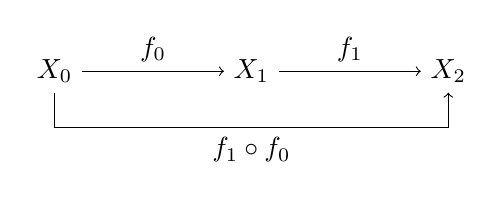
\begin{tikzpicture}[node distance=2.5cm, auto]
	\node (X) {$\bm{X_0}$};
	\node (Y) [right of=X] {$\bm{X_1}$};
	\node (n) [below of=Y,node distance=1cm] {$f_1 \circ f_0$};
	\node (Z) [right of=Y] {$\bm{X_2}$};
	\draw[->] (X) to node {$f_0$} (Y);
	\draw[->] (Y) to node {$f_1$} (Z);
%	\draw[->,bend right] (X) to node[swap] {$g \circ f$} (Z);
	\draw[->] (X) |- (n.90) -| (Z);\
\end{tikzpicture}
\end{figure}
	\end{enumerate}
\end{proposition}
\begin{proof}
\begin{enumerate}
	\item Seja $A \in \topo$. Então $\Id_X\inv(A)=A \in \topo$, logo $\Id_x$ é contínua.
	
	\item Seja $A \in \topo_2$. Como $f_1$ é contínua, $f_1\inv(A) \in \topo_1$. Como $f_0$ é contínua, $f_0\inv(f_1\inv(A)) \in \topo_0$. Portanto
		\begin{equation*}
		(f_1 \circ f_0)\inv(A) = f_1\inv \circ f_0\inv (A) = f_0\inv(f_1\inv(A)) \in \topo_0.
		\end{equation*}
	Logo $f_1 \circ f_0$ é contínua. \qedhere
\end{enumerate}
\end{proof}

\begin{definition}
Sejam $\bm{X_0}$ e $\bm{X_1}$ espaços topológicos. Um \emph{homeomorfismo} de $\bm{X_0}$ para $\bm{X_1}$ é uma função contínua $\fun{f}{\bm{X_0}}{\bm{X_1}}$ invertível cuja inversa é contínua. O conjunto de todos esses homeomorfismos é denotado por $\Iso{\Cont}(\bm{X_0},\bm{X_1})$.
Esses espaços topológicos são \emph{homeomorfos} e denota-se $\bm{X_0} \simeq \bm{X_1}$.
\end{definition}

\begin{exercise}
Sejam $\bm{X_0}$, $\bm{X_1}$ e $\bm{X_2}$ espaços topológicos.
		\begin{enumerate}
		\item (Reflexividade) $\bm{X_0} \simeq \bm{X_0}$;
		\item (Antissimetria) $\bm{X_0} \simeq \bm{X_1} \Rightarrow \bm{X_1} \simeq \bm{X_0}$;
		\item (Transitividade) $\bm{X_0} \simeq \bm{X_1} \e \bm{X_1} \simeq \bm{X_2} \Rightarrow \bm{X_0} \simeq \bm{X_2}$.
		\end{enumerate}
\end{exercise}

\subsubsection{Suporte de funções vetoriais}

\begin{definition}
Sejam $\bm X$ um espaço topológico, $\bm L$ um espaço linear topológico e $f\colon X \to L$ uma função contínua. O \emph{suporte fechado} de $f$ é o conjunto
	\begin{equation*}
	\overline\supp(f) := \Fec{\supp(f)} = \Fec{f\inv(L \setminus \{0\})}.
	\end{equation*}
\end{definition}

\subsection{Topologias induzidas}

Nesta seção estudaremos como induzir topologias em conjuntos a partir de topologias que já temos. Isso será feito, em geral, de modo que uma ou mais funções sejam contínuas e a topologia induzida seja a menor ou a maior possível, dependendo do caso. Quando temos uma função de um conjunto em um espaço topológico, podemos induzir uma topologia nesse conjunto de modo que a topologia faça com  que a função seja contínua. Nesse caso, a maior topologia que faz a função ser contínua é a topologia discreta, e o nosso interesse será achar a menor topologia tal que a função é discreta. Quando temos uma função de um espaço topológico em um conjunto, o caso se inverte. A menor topologia tal que a função é contínua sempre é a topologia trivial, e o nosso interesse está na maior topologia que garante a continuidade. De maneira parecida, podemos induzir topologias garantindo a continuidade de várias funções e também considerando funções injetivas e sobrejetivas quado necessário. O estudo desta seção envolve a definição dessas noções e a investigação inicial como sobre esses objetos se comportam e por que são os menores ou maiores com determinadas características.

\subsubsection{Topologias puxada e inicial}

\begin{definition}
Sejam $X$ um conjunto, $\bm Y = (Y,\topo_Y)$ um espaço topológico e $f: X \to Y$ uma função. A \emph{topologia puxada} por $f$ de $\bm Y$ para $X$ é
	\begin{equation*}
	f^\star(\topo_Y) := \set{f^{-1}(A)}{A \in \topo_Y}.
	\end{equation*}
\end{definition}

\begin{proposition}
Sejam $X$ um conjunto, $\bm Y = (Y,\topo_Y)$ um espaço topológico e $f: X \to Y$ uma função. Então $f^\star(\topo_Y)$, a topologia puxada por $f$ de $\bm Y$ para $X$, é uma topologia de $X$.
\end{proposition}
\begin{proof}
(1) Notemos que, como $\emptyset \in \topo_Y$ e $\emptyset = f\inv(\emptyset)$, temos que $\emptyset \in f^\star(\topo_Y)$. (2) Seja $(A_i)_{i \in I}$ uma família de conjuntos em $f^\star(\topo_Y)$. Então, para cada $i \in I$, existe aberto $U_i \in \topo_Y$ tal que $A_i=f\inv(U_i)$. Como $\topo_Y$ é topologia, a união de abertos é aberto $\bigcup_{i \in I} U_i \in \topo_Y$. Portanto
	\begin{equation*}
	\bigcup_{i \in I} A_i = \bigcup_{i \in I} f\inv(U_i) = f\inv\left( \bigcup_{i \in I} U_i\right),
	\end{equation*}
logo $\bigcup_{i \in I} A_i \in f^\star(\topo_Y)$.
(3) Seja $(A_i)_{i=1}^n$ uma família de conjuntos em $f^\star(\topo_Y)$. Então, para cada $1 \leq i \leq n$, existe aberto $U_i \in \topo_Y$ tal que $A_i=f\inv(U_i)$. Como $\topo_Y$ é topologia, a interseção finita de abertos é aberto $\bigcap_{i=1}^n U_i \in \topo_Y$. Portanto
	\begin{equation*}
	\bigcap_{i=1}^n A_i = \bigcap_{i=1}^n f\inv(U_i) = f\inv\left( \bigcap_{i=1}^n U_i\right),
	\end{equation*}
logo $\bigcap_{i=1}^n A_i \in f^\star(\topo_Y)$.
\end{proof}

\begin{proposition}
\label{topo:prop.cont.topo.pux}
Sejam $\bm X = (X,\topo_ X)$ e $\bm Y = (Y,\topo_ Y)$ espaços topológicos. Uma função $f: X \to Y$ é função contínua de $\bm X$ para $\bm Y$ se, e somente se, a topologia $f^\star(\topo_Y)$ puxada por $f$ de $\bm Y$ para $X$ é uma subtopologia de $\topo_ X$.
	\begin{equation*}
	f \in \Cont(\bm X,\bm Y) \sse f^\star(\topo_Y) \subseteq \topo_X.
	\end{equation*}
\end{proposition}
\begin{proof}
Suponha que $f \in \Cont(\bm X,\bm Y)$ e seja $B \in f^\star(\topo_Y)$. Então existe $A \in \topo_Y$ tal que $B=f\inv(A)$. Como $f$ é contínua, segue que $f\inv(A) \in \topo_X$, portanto, $f^\star(\topo_Y) \subseteq \topo_X$. Reciprocamente, suponha que $f^\star(\topo_Y) \subseteq \topo_X$. Então, para todo $A \in \topo_Y$, $f\inv(A) \in f^\star(\topo_Y)$, portanto $f\inv(A) \in \topo_X$, o que mostra que $f \in \Cont(\bm X,\bm Y)$.
\end{proof}

\begin{definition}
Sejam $\bm X$ um conjunto, $(\bm{X_i})_{i \in I} = (X_i,\topo_i)_{i \in I}$ uma família de espaços topológicos e, para todo $i \in I$, $f_i: X \to X_i$ uma função. A \emph{topologia inicial} de $X$ com respeito à família $(f_i)_{i \in I}$ é a menor topologia de $X$ tal que, para todo $i \in I$, $f_i$ é contínua.
\end{definition}

\begin{proposition}
Sejam $\bm X$ um conjunto, $(\bm{X_i})_{i \in I} = (X_i,\topo_i)_{i \in I}$ uma família de espaços topológicos e, para todo $i \in I$, $f_i: X \to X_i$ uma função. A topologia inicial de $X$ com respeito à família $(f_i)_{i \in I}$ é a topologia
	\begin{equation*}
	\ger{\bigcup_{i \in I} {f_i}^\star(\topo_i)}.
	\end{equation*}
\end{proposition}
\begin{proof}
Seja $\topo$ uma topologia de $X$ tal que, para todo $i \in I$, $f_i: X \to X_i$ é contínua. Então, para todo $i \in I$, ${f_i}^\star(\topo_i) \subseteq \topo$ (\ref{topo:prop.cont.topo.pux}), o que implica que $\bigcup_{i \in I} {f_i}^\star(\topo_i) \subseteq \topo$ e, portanto, $\ger{\bigcup_{i \in I} {f_i}^\star(\topo_i)} \subseteq \topo$.
\end{proof}

\subsubsection{Topologias empurrada e final}

\begin{definition}
Sejam $\bm X = (X,\topo_X)$ um espaço topológico, $Y$ um conjunto e $f: X \to Y$ uma função. A \emph{topologia empurrada} por $f$ de $\bm X$ para $Y$ é
	\begin{equation*}
	f_\star(\topo_X) := \set{A \subseteq Y}{f^{-1}(A) \in \topo_X}.
	\end{equation*}
\end{definition}

\begin{proposition}
Sejam $\bm X = (X,\topo_X)$ um espaço topológico, $Y$ um conjunto e $f: X \to Y$ uma função. Então $\topo_Y := f_\star(\topo_X)$, a topologia empurrada por $f$ de $\bm X$ para $Y$, é uma topologia de $Y$.
\end{proposition}
\begin{proof}
(1) Como $f\inv(\emptyset)=\emptyset$ e $f\inv(Y)=X$, segue que $\emptyset,Y \in f_\star(\topo_X)$. (2) Seja $(A_i)_{i \in I}$ uma família de conjuntos de $f_\star(\topo_X)$. Então, para cada $i \in I$, $f\inv(A_i) \in \topo_X$, o que implica que
\begin{equation*}
	f\inv \left( \bigcup_{i \in I} A_i \right) = \bigcup_{i \in I} f\inv(A_i) \in \topo_X,
	\end{equation*}
portanto $\bigcup_{i \in I} A_i \in f_\star(\topo_X)$. (3) Seja $(A_i)_{i=1}^n$ uma família de conjuntos de $f_\star(\topo_X)$. Então, para cada $1 \leq i \leq n$, $f\inv(A_i) \in \topo_X$, o que implica que
\begin{equation*}
	f\inv \left( \bigcap_{i=1}^n A_i \right) = \bigcap_{i=1}^n f\inv(A_i) \in \topo_X,
	\end{equation*}
portanto $\bigcap_{i=1}^n A_i \in f_\star(\topo_X)$.
\end{proof}

\begin{definition}
Sejam $\bm X$ um conjunto, $(\bm{X_i})_{i \in I} = (X_i,\topo_i)_{i \in I}$ uma família de espaços topológicos e, para todo $i \in I$, $f_i: X_i \to X$ uma função. A \emph{topologia final} de $X$ com respeito à família $(f_i)_{i \in I}$ é a maior topologia de $X$ tal que, para todo $i \in I$, $f_i$ é contínua.
\end{definition}

\begin{proposition}
Sejam $\bm X$ um conjunto, $(\bm{X_i})_{i \in I} = (X_i,\topo_i)_{i \in I}$ uma família de espaços topológicos e, para todo $i \in I$, $f_i: X_i \to X$ uma função. A topologia final de $X$ com respeito à família $(f_i)_{i \in I}$ é a topologia
	\begin{equation*}
	\bigcap_{i \in I} {f_i}_\star(\topo_i).
	\end{equation*}
\end{proposition}
\begin{proof}
Seja $\topo$ uma topologia de $X$ tal que, para todo $i \in I$, $f_i: X_i \to X$ é contínua, e seja $A \in \topo$. Então, para todo $i \in I$, $f_i \inv(A) \in \topo_i$, o que implica que $A \in {f_i}_\star(\topo_i)$, portanto $A \in \bigcap_{i \in I} {f_i}_\star(\topo_i)$. Isso mostra que $\topo \subseteq \bigcap_{i \in I} {f_i}_\star(\topo_i)$, e como interseção de topologias é topologia, segue o procurado.
\end{proof}

\subsubsection{Produto de espaços topológicos}

\begin{definition}
Seja $(\bm{X_i})_{i \in I} = (X_i,\topo_i)_{i \in I}$ uma família de espaços topológicos. O \emph{produto} da família $(\bm{X_i})_{i \in I}$ é o par
	\begin{equation*}
	\prod_{i \in I} \bm{X_i} := \left( \prod_{i \in I} X_i , \ger{\bigcup_{i \in I}{\pi_i}^\star(\topo_i)} \right).
	\end{equation*}
A topologia $\ger{\bigcup_{i \in I}{\pi_i}^\star(\topo_i)}$ é a \emph{topologia produto} de $\prod_{i \in I} X_i$.
\end{definition}

\begin{proposition}
Sejam $(\bm{X_i})_{i \in I} = (X_i,\topo_i)_{i \in I}$ uma família de espaços topológicos e $X = \prod_{i \in I} X_i$ o produto de conjuntos. A topologia produto de $X$ é a topologia gerada pela base cujos elementos são $\prod_{i \in I} A_i$, tal que $A_i \in \topo_i$ e existe $J \subseteq I$ finito com $A_i = X_i$ para $i \in I \setminus J$.
\end{proposition}
\begin{proof}
Como $\pi_i = \pi_i \circ \Id_X$, segue de uma propriedades básica de imagem inversa de produto (\ref{conj:prop.im.inv.prod}) que
	\begin{equation*}
	\prod_{i \in I} A_i = \Id_X\inv \left(\prod_{i \in I} A_i\right) = \bigcap_{i \in I} \pi_i\inv(A_i)
	\end{equation*}
Para todo $i \in I \setminus J$, $A_i=X_i$, então $\pi_i\inv(A_i)=X$ e, portanto,
	\begin{equation*}
	\bigcap_{i \in I\setminus J} \pi_i\inv(A_i) = \bigcap_{i \in I\setminus J} X = X.
	\end{equation*}
Isso implica que
	\begin{equation*}
	\bigcap_{i \in I} \pi_i\inv(A_i) = \left(\bigcap_{i \in I\setminus J} \pi_i\inv(A_i)\right) \cap \left(\bigcap_{j \in J} \pi_j\inv(A_j)\right) =  \bigcap_{j \in J} \pi_j\inv(A_j)
	\end{equation*}
Logo $\prod_{i \in I} A_i = \bigcap_{j \in J} \pi_j\inv(A_j)$. Seja $A$ aberto da topologia descrita na proposição. Então
	\begin{equation*}
	A = \bigcup_{k \in K} A_k = \bigcup_{k \in K}\prod_{i \in I} A_{ki} = \bigcup_{k \in K}\bigcap_{j \in J} \pi_j\inv (A_{kj}),
	\end{equation*}
o que mostra que $A$ é aberto da topologia produto. O resto da demonstração é simples.
\end{proof}

\begin{proposition}[Propriedade Universal]
Sejam $(\bm{X_i})_{i \in I} = (X_i,\topo_i)_{i \in I}$ uma família de espaços topológicos, $\bm T = (T,\topo_T)$ um espaço topológico e, para todo $i \in I$, $f_i: \bm T \to \bm{X_i}$ uma função contínua. Então existe uma única função contínua $f: \bm T \to \prod_{i \in I} \bm{X_i}$ tal que, para todo $i \in I$, $\pi_i \circ f = f_i$ (o diagrama comuta).
\begin{figure}
\centering
\begin{tikzpicture}[node distance=2.5cm, auto]
	\node (P) {$\displaystyle\prod_{i \in I} \bm{X_i}$};
	\node (Ci) [below of=P] {$\bm{X_i}$};
	\node (X) [left of=Ci] {$\bm{T}$};
	\draw[->] (X) to node [swap] {$f_i$} (Ci);
	\draw[->, dashed] (X) to node {$f$} (P);
	\draw[->] (P) to node {$\pi_i$} (Ci);
\end{tikzpicture}
\end{figure}
\end{proposition}
\begin{proof}
Defina a função
	\begin{align*}
	\func{f}{T}{ \prod_{i \in I} X_i}{ x}{ (f_i(x))_{i \in I}}.
	\end{align*}
Pela propriedade universal do produto de conjuntos, $f$ é única e $\pi_i \circ f = f_i$. Resta mostrar que $f$ é contínua. Seja $A \in \topo_X$. Então $A=\bigcup_{k \in K} A_k$ é uma união de abertos básicos $A_k \in \topo$. Isso significa que, para todo $k \in K$, $A_k = \prod_{i \in I} A_{ki}$, com $A_{ki} \in \topo_i$ para todo $i \in I$ e existe $J_k \subseteq I$ finito tal que, para todo $i \in I \setminus J_k$, $A_{ki} = X_i$. Assim, por propriedades básicas de imagem inversa de união e produto (\ref{conj:prop.im.inv.prod}),
		\begin{equation*}
		f\inv(A) = f\inv\left(\bigcup_{k \in K}\prod_{i \in I} A_{ki}\right) = \bigcup_{k \in K} f\inv \left( \prod_{i \in I} A_{ki} \right) = \bigcup_{k \in K}\bigcap_{i \in I}f_i\inv(A_{ki}).
		\end{equation*}
Seja $k \in K$. Como, para todo $i \in I \setminus J_k$, $A_{ki} = X_i$, então $f_i\inv(A_{ki}) = f_i\inv(X_i) = T$. Disso segue que
	\begin{equation*}
	\bigcap_{i \in I}f_i\inv(A_{ki}) = \bigcap_{j \in J_k}f_j\inv(A_{kj})
	\end{equation*}
e, portanto,
	\begin{equation*}
	f\inv(A) = \bigcup_{k \in K}\bigcap_{j \in J_k}f_j\inv(A_{kj}).
	\end{equation*}
Seja $k \in K$. Para todo $j \in J_k$, $f_j$ é contínua, o que implica que $f_j\inv(A_{kj})$ é aberto e, por $J_k$ ser finito, a interseção $\bigcap_{j \in J_k}f_j\inv(A_{kj})$ é aberta. Isso significa que a união $\bigcup_{k \in K}\bigcap_{j \in J_k}f_j\inv(A_{kj})$ é aberta e, portanto, $f\inv(A) \in \topo_T$. Logo $f$ é contínua.
\end{proof}

\subsubsection{Coproduto de espaços topológicos}

\begin{definition}
Seja $(\bm{X_i})_{i \in I} = (X_i,\topo_i)_{i \in I}$ uma família de espaços topológicos. O \emph{coproduto} da família $(\bm{X_i})_{i \in I}$ é o par
	\begin{equation*}
	\coprod_{i \in I} \bm{X_i} := \left( \coprod_{i \in I} X_i , \bigcap_{i \in I}{\iota_i}_\star(\topo_i) \right).
	\end{equation*}
A topologia $\bigcap_{i \in I}{\pi_i}_\star(\topo_i)$ é a \emph{topologia coproduto} de $\coprod_{i \in I} X_i$.
\end{definition}

\begin{proposition}[Propriedade Universal]
Sejam $(\bm{X_i})_{i \in I} = (X_i,\topo_i)_{i \in I}$ uma família de espaços topológicos, $\bm T = (T,\topo_T)$ um espaço topológico e, para todo $i \in I$, $f_i: \bm{X_i} \to \bm T$ uma função contínua. Então existe uma única função contínua $f: \coprod_{i \in I} \bm{X_i} \to \bm T$ tal que, para todo $i \in I$, $f \circ \iota_i = f_i$ (o diagrama comuta).
\begin{figure}
\centering
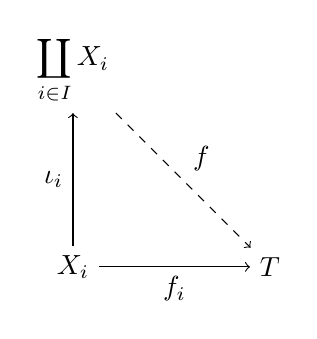
\begin{tikzpicture}[node distance=2.5cm, auto]
	\node (Ci) {$\bm{X_i}$};
	\node (S) [above of=Ci] {$\displaystyle\coprod_{i \in I} \bm{X_i}$};
	\node (X) [right of=Ci] {$\bm T$};
	\draw[->] (Ci) to node [swap] {$f_i$} (X);
	\draw[->, dashed] (S) to node {$f$} (X);
	\draw[->] (Ci) to node {$\iota_i$} (S);
\end{tikzpicture}
\end{figure}
\end{proposition}

\subsubsection{Subespaços topológicos}

\begin{definition}
Sejam $(X,\topo)$ um espaço topológico e $S \subseteq X$ um subconjunto. A \emph{topologia induzida} por $\topo$ em $S$ é o conjunto
	\begin{equation*}
	\topo|_S := \set{A \cap S}{A \in \topo}.
	\end{equation*}
\end{definition}

\begin{proposition}
Sejam $(X,\topo)$ um espaço topológico e $S \subseteq X$ um subconjunto. A topologia induzida por $\topo$ em $S$ é o conjunto
	\begin{equation*}
	\topo|_S = \iota_\star(\topo),
	\end{equation*}
a maior topologia tal que a inclusão $\iota: S \to X$ é contínua.
\end{proposition}

\begin{proposition}
Sejam $(X,\topo)$ um espaço topológico e $S \subseteq X$ um subconjunto. A topologia induzida por $\topo$ em $S$ é uma topologia de $S$.
\end{proposition}
\begin{proof}
(1) Notemos que $\emptyset,S \in \topo|_S$, pois $\emptyset \cap S = \emptyset$ e $X \cap S = S$. (2) Seja $(A_i)_{i \in I}$ uma família de abertos de $\topo|_S$. Então, para cada $i \in I$, existe um aberto $B_i \in \topo$ tal que $A_i = B_i \cap S$. Assim, temos que
	\begin{equation*}
	\bigcup_{i \in I} A_i = \bigcup_{i \in I} (B_i \cap S) = \left( \bigcup_{i \in I} B_i \right) \cap S,
	\end{equation*}
que pertence à topologia induzida pois $\bigcup_{i \in I} B_i \in \topo$. (3) Seja $(A_i)_{i=1}^n$ uma família de abertos de $\topo|_S$. Então, para cada $1 leq i leq n$, existe um aberto $B_i \in \topo$ tal que $A_i = B_i \cap S$. Assim, temos que
	\begin{equation*}
	\bigcap_{i=1}^n A_i = \bigcap_{i=1}^n (B_i \cap S) = \left( \bigcap_{i=1}^n B_i \right) \cap S,
	\end{equation*}
que pertence à topologia induzida pois $\bigcap_{i=1}^n B_i \in \topo$.
\end{proof}

\begin{proposition}[Propriedade característica]
Sejam $\bm X=(X,\topo_X)$ e $(Y,\topo_Y)$ espaços topológicos e $\bm S \subseteq \bm X$ um subespaço. Uma função $f\colon Y \to S$ é contínua se, e somente se, $\iota \circ f: Y \to X$ é contínua (o diagrama comuta).
\begin{figure}
\centering
\begin{tikzpicture}[node distance=2.5cm, auto]
	\node (X) {$\bm X$};
	\node (S) [below of=X] {$\bm S$};
	\node (Y) [left of=S] {$\bm{T}$};
	\draw[->] (Y) to node [swap] {$f$} (S);
	\draw[->] (Y) to node {$\iota \circ f$} (X);
	\draw[->] (S) to node [swap] {$\iota$} (X);
\end{tikzpicture}
\end{figure}
\end{proposition}

\paragraph*{Proposição} Restrição de função contínua é contínua na topologia induzida.

\begin{proposition}[Colagem por abertos]
Sejam $\bm X$ e $\bm Y$ espaços topológicos, $f: X \to Y$ uma função e $(X_i)_{i \in I}$ uma cobertura de $X$ por conjuntos abertos tal que, para todo $i \in I$, $f|_{X_i}: X_i \to Y$ é contínua. Então $f: X \to Y$ é contínua.
\end{proposition}

\begin{proposition}[Colagem por fechados]
Sejam $\bm X$ e $\bm Y$ espaços topológicos, $f: X \to Y$ uma função e $(X_i)_{i=1}^n$ uma cobertura de $X$ por conjuntos fechados tal que, para todo $1 \leq i \leq n$, $f|_{X_i}: X_i \to Y$ é contínua. Então $f: X \to Y$ é contínua.
\end{proposition}

\subsubsection{Quociente de espaços topológicos}

\begin{definition}
Sejam $\bm X = (X,\topo)$ um espaço topológico e $\sim$ uma relação de equivalência em $X$. O \emph{espaço quociente} com respeito a $\sim$ é o espaço topológico
	\begin{equation*}
	\bm{\quo{X}{\sim}} := \left( \quo{X}{\sim}, \pi^\star(\topo) \right),
	\end{equation*}
em que $\pi: X \to \quo{X}{\sim}$ é a projeção canônica de equivalências.
\end{definition}

É fácil notar que os abertos de $\bm{\quo{X}{\sim}}$ são conjuntos de classes de equivalência cuja união é um aberto de $\bm X$. Notemos, ainda, que se $f: X \to Y$ é sobrejetivo, existe uma relação de equivalência em $X$ induzida por $f$, definida como dois elementos são equivalentes se suas imagens são iguais, e essa relação de equivalência faz com que possamos identificar $Y$ com $\quo{X}{\sim}$ como conjuntos. Definimos a topologia em $Y$ de modo que $Y$ e $\quo{X}{\sim}$ sejam homeomorfos.

\begin{proposition}[Propriedade característica]
Sejam $\bm X=(X,\topo_X)$ e $(Y,\topo_Y)$ espaços topológicos e $\bm Q$ um espaço quociente de $\bm X$. Uma função $f: Q \to Y$ é contínua se, e somente se, $f \circ \pi: X \to Y$ é contínua (o diagrama comuta).
\begin{figure}
\centering
\begin{tikzpicture}[node distance=2.5cm, auto]
	\node (Q) {$\bm Q$};
	\node (X) [above of=Q] {$\bm X$};
	\node (Y) [right of=Q] {$\bm Y$};
	\draw[->] (Q) to node [swap] {$f$} (Y);
	\draw[->] (X) to node {$f \circ \pi$} (Y);
	\draw[->] (X) to node [swap] {$\pi$} (Q);
\end{tikzpicture}
\end{figure}
\end{proposition}

\subsection{Topologia de ordem}

Lembremos que, se $(X,\leq)$ é um conjunto (totalmente) ordenado e $e,e' \in X$, o intervalo aberto de extremos inferior $e$ e superior $e'$ é o conjunto
	\begin{equation*}
	\intaa{e}{e'}= \set{x \in X}{e < x < e'}.
	\end{equation*}
As semirretas abertas são os intervalos
	\begin{equation*}
	\intaa{e}{\infty} := \set{x \in X}{e < x}
	\end{equation*}
e
	\begin{equation*}
	\intaa{-\infty}{e} := \set{x \in X}{x < e}.
	\end{equation*}

%Definindo a função $m_e(x) = \min\{x,e\}$. Então
%	\begin{equation*}
%	\intaa{-\infty}{e} = {m_e}\inv(X).
%	\end{equation*}

\begin{definition}
Seja $(X,\leq)$ um conjunto ordenado. A \emph{topologia de ordem} sobre $X$ é a topologia gerada pelas semirretas abertas de $(X,\leq)$. %pelos intervalos abertos $\intaa{e}{e'}$.
Denotamos essa topologia por $\topo_\leq$ (ou simplesmente $\topo$ se for claro pelo contexto).
\end{definition}

\begin{proposition}
Seja $(X,\leq)$ um conjunto ordenado. O par $(X,\topo_\leq)$ é um espaço topológico hereditariamente normal com base de intervalos abertos.
\end{proposition}

\subsubsection{Topologia de um corpo ordenado}

Lembremos que, se $(X,\leq)$ é um espaço ordenado, a topologia $\topo_\leq$ induzida por $\leq$ é a topologia gerada pelas semirretas abertas $\intaa{x}{\infty}$ e $\intaa{\infty}{x}$, e o conjunto de intervalos abertos $\intaa{x}{x'}$ é uma base de $\topo_\leq$.

Note que
	\begin{align*}
	\bigcup_{i \in I} \intaa{e_i}{e'_i} &= \intaa{\inf_{i \in I} e_i}{\sup_{i \in I} e'_i} \\
	\bigcap_{i \in I} \intff{e_i}{e'_i} &= \intff{\sup_{i \in I} e_i}{\inf_{i \in I} e'_i}.
	\end{align*}

\begin{proposition}
Seja $(\bm C,\leq)$ um corpo ordenado. O par $(\bm C,\topo_\leq)$ é um corpo topológico.
\end{proposition}
\begin{proof}
Precisamos mostrar que $+$, $-$, $\times$ e $\inv$ são contínuas. Para isso, basta mostrar que elas puxam abertos geradores para abertos. Seja $e \in C$ e consideremos as semirretas $\intaa{e}{\infty}$ e $\intaa{-\infty}{e}$. Para mostrar que $+$ é contínua, notamos que, se $c+c' > e$, então $c' > e-c$, logo
	\begin{equation*}
	+\inv \big( \intaa{e}{\infty} \big) = \bigcup_{c \in C} \big( \intaa{c}{\infty} \times \intaa{e-c}{\infty} \big)
	\end{equation*}
e, analogamente,
	\begin{equation*}
	+\inv \big( \intaa{-\infty}{e} \big) = \bigcup_{c \in C} \big( \intaa{-\infty}{c} \times \intaa{-\infty}{e-c} \big),
	\end{equation*}
que são abertos pois são uniões de abertos, o que implica que $+$ é contínua. Para mostrar que $-$ é contínua, notamos que
	\begin{equation*}
	-\inv \big( \intaa{e}{\infty} \big) = \intaa{-\infty}{-e}
	\end{equation*}
e
	\begin{equation*}
	-\inv( \intaa{-\infty}{e} ) = \intaa{-e}{\infty},
	\end{equation*}
que são ambos abertos, o que mostra que $-$ é contínua.

Para mostrar que $\times$ é contínua, consideramos dois casos. 

(1) Se $e=0$ e $c \times c' > e=0$, então $c \neq 0$, logo se $c > 0$ então $c'>0$ e, se $c < 0$, então $c' < 0$, logo
	\begin{equation*}
	\times\inv \big( \intaa{0}{\infty} \big) = \big( \intaa{0}{\infty} \times \intaa{0}{\infty} \big) \cup \big( \intaa{-\infty}{0} \times \intaa{-\infty}{0} \big)
	\end{equation*}
e, analogamente,
	\begin{equation*}
	\times\inv \big( \intaa{-\infty}{0} \big) = \big( \intaa{0}{\infty} \times \intaa{-\infty}{0} \big) \cup \big( \intaa{-\infty}{0} \times \intaa{0}{\infty} \big),
	\end{equation*}
que são ambos abertos;
%	\begin{equation*}
%	\times\inv ( \intaa{0}{\infty} ) = \bigcup_{c \in C_{>0}} \big( \intaa{c}{\infty} \times \intaa{0}{\infty} \big) \cup \bigcup_{c \in C_{<0}} \big( \intaa{\infty}{c} \times \intaa{-\infty}{0} \big)
%	\end{equation*
%(2) se $e > 0$ e $c \times c' > e > 0$, então $c \neq 0$,
%
%notamos que, se $c \times c' > e$, existem dois casos: (1) se $e=0$, então $c \neq 0$, logo $c' > c$
%
%
%(1) se $c \neq 0$, então $c' \geq e/c$; se $c=0$, então e caso contr
%
%
%	\begin{equation*}
%	\times\inv ( \intaa{e}{\infty} ) = \bigcup_{c \in C \setminus \{0\}} \intaa{c}{\infty} \times \intaa{e/c}{\infty}
%	\end{equation*}
%pois
o caso (2) em que $e \neq 0$ é análogo, embora um pouco mais trabalhoso. Isso mostra que $\times$ é contínua. Mostrar que $\inv$ é contínua também é trabalhoso, mas segue direto de modo análogo.
%Para mostrar que $/$ é contínua, notamos que
%	\begin{equation*}
%	{/}\inv \big( \intaa{0}{\infty} \big)
%	\end{equation*}
\end{proof}



% Topologicamente falando, qual a consequência de um corpo ser infinitesimal/arquimediano?




\begin{proposition}
Seja $(\bm C,\leq)$ um corpo ordenado. O corpo topológico $(\bm C,\topo_\leq)$ é separado.
\end{proposition}
\begin{proof}
Sejam $c,c' \in C$ tais que $c \neq c'$. Então $c < c'$ ou $c' < c$. Sem perda de generalidade, considere que $c < c'$. Então as vizinhanças
	\begin{equation*}
	\intaa{-\infty}{\frac{c+c'}{2}} \qquad\text{e}\qquad \intaa{\frac{c+c'}{2}}{\infty}
	\end{equation*}
de $c$ e $c'$, respectivamente, separam $c$ e $c'$.
\end{proof}

% MOSTRAR QUE É NORMAL
%Qualquer aberto é da forma
%	\begin{equation*}
%	\bigcup_{i \in I} \intaa{e_i}{e'_i},
%	\end{equation*}
%em que $e_i < e'_i$, mas $e_i,e'_i$ podem ser, respectivamente, $-\infty$ e $\infty$. Isso implica que qualquer fechado é da forma
%	\begin{align*}
%	F = \left( \bigcup_{i \in I} \intaa{e_i}{e'_i} \right)^\complement &= \bigcap_{i \in I} \big( \intaa{e_i}{e'_i} \big)^\complement \\
%		&= \bigcap_{i \in I} \big( \intaa{-\infty}{e_i} \cup \intaa{e'_i}{\infty} \big) \\
%%		&= \left( \bigcap_{i \in I} \intaa{-\infty}{e_i} \right) \cup \left( \bigcap_{i \in I}\intaa{e'_i}{\infty} \right) \\
%%		&= 
%	\end{align*}
%
%Agora, seja $c \notin F$. Então $c \in \bigcup_{i \in I} \intaa{e_i}{e'_i}$, o que significa que existe algum $i \in I$ tal que $c \in \intaa{e_i}{e'_i}$.

% Tem no stack exchange como mostrar que todo espaço métrico é completamente normal, deve dar pra estender pra espaços "métricos" com uma distância a valores no cone positivo de um corpo ordenado.

Consideremos em $C_{\geq 0}$ a topologia induzida.

\begin{proposition}
Seja $(\bm C,\leq)$ um corpo ordenado. As funções valor absoluto $\abs{\var}\colon C \to C_{\geq 0}$ e distância $\dist{\var}{\var}\colon C \times C \to C_{\geq 0}$ são contínuas.
\end{proposition}
\begin{proof}
(Valor absoluto) Seja $c \in C_{\geq 0}$ e consideremos os abertos $\intaa{c}{\infty}$ e $\intfa{0}{c}$. Então
	\begin{equation*}
	\abs{\var}\inv \big( \intaa{c}{\infty} \big) = \intaa{-\infty}{-c} \cup \intaa{c}{\infty}
	\end{equation*}
e
	\begin{equation*}
	\abs{\var}\inv \big( \intfa{0}{c} \big) = \intaf{-c}{0} \cup \intfa{0}{c} = \intaa{-c}{c},
	\end{equation*}
que são ambos abertos, o que mostra que $\abs{\var}$ é contínua.

(Distância) Como $\dist{\var}{\var}$ é composição de $\abs{\var}$, $+$, $-$, $\proj_0$ e $\proj_1$, que são todas contínuas, segue que ela é contínua.
%	\begin{equation*}
%	\dist{c}{c'} := \abs{c'-c}
%	\end{equation*}
%	\begin{align*}
%	\dist{\var}{\var} &= \dist{\var}{\var} \circ \Id \\
%		&= \dist{\var}{\var} \circ (\proj_0,\proj_1) \\
%		&= \dist{\proj_0}{\proj_1} \\
%		&= \abs{\proj_1-\proj_0} \\
%		&= \abs{\var} \circ (+(\proj_1,- \circ \proj_0)).
%	\end{align*}
\end{proof}





\begin{proposition}
Seja $(\bm C,\leq)$ um corpo ordenado. O corpo $\bm C$ é não-infinitesimal se, e somente se, $\Q_C$ é denso em $C$.
\end{proposition}

\section{Separação}

\subsection{Noções de separação de conjuntos}

Nesta seção são apresentadas algumas noções de como dois conjuntos de um espaço topológico podem ser separados. As duas noções mas simples de separação são noções conjuntistas. A primeira é a de conjuntos distintos, ou diferentes, $A \neq B$, e a outra é a de conjuntos disjuntos, $A \cap B = \emptyset$. A seguir, mostramos noções que envolvem construções topológicas e não meramente conjuntistas.

\begin{definition}
Sejam $\bm X$ um espaço topológico e $A,B \subseteq X$. Definimos as seguintes relações entre $A$ e $B$:
	\begin{enumerate}
	\item (\emph{Separação}) Cada conjunto é disjunto do fecho do outro.
	\begin{equation*}
	A \cap \Fec{B} = \Fec{A} \cap B = \emptyset.
	\end{equation*}
	\item (\emph{Separação por vizinhanças}) Existem vizinhanças $V_A \in \viz_A$ e $V_B \in \viz_B$ que são disjuntas.
	\begin{equation*}
	V_A \cap V_B = \emptyset.
	\end{equation*}
	\item (\emph{Separação por função contínua}) Existe uma função contínua $f \in \Cont(X,[0,1])$ tal que
	\begin{equation*}
	f(A)=\{0\} \e f(B)=\{1\}.
	\end{equation*}
	\item (\emph{Separação precisa por função contínua}) Existe uma função contínua $f \in \Cont(X,[0,1])$ tal que
	\begin{equation*}
	f\inv(\{0\})=A \e f\inv(\{1\})=B.
	\end{equation*}
	\end{enumerate}
Cada uma das relações vale entre pontos $x,y \in X$, ou entre um conjunto $A$ e um ponto $x$, ao considerarmos no lugar no ponto o conjunto unitário que o contém: valem entre os conjuntos $\{x\}$ e $\{y\}$, ou entre $A$ e $\{x\}$, respectivamente.
\end{definition}

	As primeiras duas relações binárias são claramente simétricas, mas isso não é necessariamente claro no caso da terceira e quarta. No entanto, isso pode ser concluído ao considerar, dada uma função $f$ que faz $A$ e $B$ separados por função contínua, a função $1-f$ que faz o mesmo entre $B$ e $A$.

\begin{proposition}
\label{topo:prop.separacao}
Sejam $\bm X$ um espaço topológico e $A,B \subseteq X$. Então
	\begin{enumerate}
	\item Se $A$ e $B$ são precisamente separados por função contínua, então são separados por função contínua.
	\item Se $A$ e $B$ são separados por função contínua, então são separados por vizinhanças.
	\item Se $A$ e $B$ são separados por vizinhanças, então são separados.
	\item Se $A$ e $B$ são separados, então são disjuntos.
	\end{enumerate}
\end{proposition}
%\begin{proof}
%Suponhamos que existe função contínua $f:X \to [0,1]$ tal que $f(A)= \{0\}$ e $f(B)=\{1\}$. Definamos $U := f^{-1}(\left[0,\frac{1}{2}\right))$ e $V := f^{-1}((\frac{1}{2},1))$. Como $f$ é contínua, $U$ e $V$ são abertos. Ainda, $A \subseteq U$ e $B \subseteq V$. Por fim, como $U \cap V = \emptyset$, concluímos que $\bm X$ é normal.
%\end{proof}

% DÚVIDA: As relações de separação negadas são relações de equivalência? Pois indintinguibilidade topológica é, e ela é a negação de separação de pontos (não exatamente). Tentar entender melhor isso.


\subsection{Espaços distinguíveis}

\begin{definition}
Seja $\bm X$ um espaço topológico. Pontos \emph{topologicamente indistinguíveis} em $\bm X$ são pontos $x,y \in X$ tais que $\viz_x = \viz_y$. Pontos \emph{topologicamente disntinguíveis em $\bm X$} são pontos que não são topologicamente indistinguíveis.
\end{definition}

\begin{proposition}
Seja $\bm X$ um espaço topológico. A relação binária de indistinguibilidade topológica é uma relação de equivalência em $X$.
\end{proposition}
\begin{proof}
Denotemos por $\sim$ a relação binária de indistinguibilidade topológica. Sejam $x,y,z \in X$. Para mostrar a reflexividade, notemos que, como $\viz_x=\viz_y$, então $x \sim x$. Para mostrar a simetria, se $x \sim y$, então $\viz_x=\viz_y$, o que é equivalente a $\viz_y=\viz_x$ e, portanto, $y \sim x$. Por fim, para mostrar a transitividade, se $x \sim y$ e $y \sim z$, então $\viz_x=\viz_y$ e $\viz_y=\viz_z$, o que implica $\viz_x=\viz_z$ e, portanto, $x \sim z$.
\end{proof}

O fato de que essa é uma relação de equivalência mostra que podemos obter a partir de qualquer espaço topológico um espaço topológico em que nenhum ponto é topologicamente indisntinguível. Para isso, basta considerar o espaço quociente definido pela relação. de indistinguibilidade topológica. Espaços com essa propriedade são definidos a seguir.

\begin{definition}[$T_0$]
Um espaço topológico \emph{distinguível} é um espaço topológico $\bm X$ em que todo par de pontos distintos é topologicamente distinguível:
	\begin{equation*}
	\forall x,y \in X \quad x \neq y \quad \Rightarrow \quad \viz_x \neq \viz_y.
	\end{equation*}
\end{definition}

\begin{proposition}
Seja $\bm X$ um espaço topológico. São equivalentes as seguintes propriedades:
	\begin{enumerate}
	\item $\bm X$ é distinguível.
	\item $\forall x,y \in X \quad x \neq y \quad \Rightarrow \quad \viz_x \nsubseteq \viz_y \ou \viz_y \nsubseteq \viz_x$.
	\item $\forall x,y \in X \quad x \neq y \quad \Rightarrow \quad x \notin \Fec{\{y\}} \ou y \notin \Fec{\{x\}}$.
	\item $\forall x,y \in X \quad x \neq y \quad \Rightarrow \quad \Fec{\{x\}} \neq \Fec{\{y\}}$.	
\end{enumerate}
\end{proposition}

\begin{proposition}
Sejam $\bm X$ um espaço topológico distinguível e $Y \subseteq X$. Então $\bm Y$ é um espaço topológico distinguível.
\end{proposition}

\begin{proposition}
Seja $(X_i)_{i \in I}$ uma família não vazia de espaços topológicos não vazios. O espaço produto $\prod_{i \in I} \bm{X_i}$ é distinguível se, e somente se, todos os espaços $\bm X_i$ são distinguíveis.
\end{proposition}

\subsection{Espaços acessíveis}

\begin{definition}[$T_1$]
Um espaço topológico \emph{acessível} é um espaço topológico $\bm X$ em que
	\begin{equation*}
	\forall x,y \in X \quad x \neq y \quad \Rightarrow \quad \viz_x \nsubseteq \viz_y \e \viz_y \nsubseteq \viz_x.
	\end{equation*}
\end{definition}

\begin{proposition}[$T_1 \Rightarrow T_0$]
Seja $\bm X$ um espaço topológico. Se $\bm X$ é acessível, então $\bm X$ é distinguível.
\end{proposition}
\begin{proof}
Se $\bm X$ é acessível, então, para todos $x,y \in X$ tais que $x \neq y$, temos que $\viz_x \nsubseteq \viz_y \e \viz_y \nsubseteq \viz_x$. Mas isso implica que $\viz_x \nsubseteq \viz_y \ou \viz_y \nsubseteq \viz_x$, o que é equivalente a $\viz_x \neq \viz_y$. Logo $\bm X$ é distinguível.
\end{proof}

\begin{proposition}
Seja $\bm X$ um espaço topológico. São equivalentes as seguintes propriedades:
	\begin{enumerate}
	\item $\bm X$ é acessível.
	\item Todo par de pontos distintos é separado:
		\begin{equation*}
		\forall x,y \in X \quad x \neq y \quad \Rightarrow \quad x \notin \Fec{\{y\}} \e y \notin \Fec{\{x\}}.
		\end{equation*}
	\item $\forall x,y \in X \quad x \neq y \quad \Rightarrow \quad \exists U \in \viz_x,\ V \in \viz_y \qquad y \notin U \e x \notin V$.
	\item $\forall x \in X \quad \Fec{\{x\}}=\{x\}$.
	\end{enumerate}
\end{proposition}

\begin{proposition}
Sejam $\bm X$ um espaço topológico acessível e  $Y \subseteq X$. Então $\bm Y$ é um espaço topológico acessível.
\end{proposition}

\begin{proposition}
Seja $(X_i)_{i \in I}$ uma família não vazia de espaços topológicos não vazios. O espaço produto $\prod_{i \in I} \bm{X_i}$ é acessível se, e somente se, todos os espaços $\bm X_i$ são acessíveis.
\end{proposition}

\subsection{Espaços separados}

\begin{definition}[$T_2$]
Um espaço topológico \emph{separado (por vizinhanças)} é um espaço topológico $\bm X$ em que todo par de pontos distintos é separado por vizinhanças:
	\begin{equation*}
	\forall x,y \in X \quad x \neq y \quad \Rightarrow \quad \exists U \in \viz_x,\ V \in \viz_y \quad U \cap V = \emptyset.
	\end{equation*}
\end{definition}
Esses espaços também são conhecidos como espaços de Hausdorff.

\begin{proposition}[$T_2 \Rightarrow T_1$]
Seja $\bm X$ um espaço topológico. Se $\bm X$ é separado, então $\bm X$ é acessível.
\end{proposition}

\begin{proposition}
Seja $\bm X$ um espaço topológico. São equivalentes as seguintes propriedades:
	\begin{enumerate}
	\item $\bm X$ é separado.
	\item Toda rede convergente em $\bm X$ tem limite único.
	\item Todo filtro convergente em $\bm X$ tem limite único.
	\end{enumerate}
\end{proposition}

\begin{proposition}
Sejam $\bm X$ um espaço topológico separado e $Y \subseteq X$. Então $\bm Y$ é um espaço topológico separado.
\end{proposition}

\begin{proposition}
Seja $(\bm X_i)_{i \in I}$ uma família não vazia de espaços topológicos não vazios. O espaço produto $\prod_{i \in I} \bm{X_i}$ é separado se, e somente se, todos os espaços $\bm X_i$ são separados.
\end{proposition}

\begin{proposition}
Sejam $\bm X$ um espaço topológico, $\bm Y$ um espaço topológico separado, $D \subseteq X$ um subconjunto denso em $X$ e $f,g: X \to Y$ funções contínuas tais que $f|_D=g|_D$. Então $f=g$.
\end{proposition}

\subsection{Espaços regulares}

\begin{definition}
Um espaço topológico \emph{regular} é um espaço topológico
% $\bm X$
em que é possível separar por vizinhanças qualquer ponto de qualquer conjunto fechado que não o contém.
%: para todo $x \in X$ e para todo conjunto fechado $F \subseteq X$,
%	\begin{equation*}
%	F \cap \{x\}=\emptyset \quad \Rightarrow \quad \exists U \in \viz_x, \exists V \in \viz_F \quad U \cap V = \emptyset.
%	\end{equation*}
\end{definition}

Espaços separados regulares são também chamados de $T_3$.

\begin{proposition}
Seja $\bm X$ um espaço topológico regular. Então $\bm X$ é separado por vizinhanças se, e somente se, é distinguível.
\end{proposition}
\begin{proof}
Sabemos que todo espaço separado por vizinhanças é distinguível. Para demonstrar a recíproca, supondo que $\bm X$ é distinguível, então para todos pontos $x,y \in X$, $x \notin \Fec{\{y\}}$ ou $y \notin \Fec{\{x\}}$. Sem perda de generalidade, assumamos o primeiro caso. Seja $F := \Fec{\{y\}}$. Então $F$ é fechado e $x \notin F$. Da regularidade de $\bm X$, segue que existem $U \in \viz_x$ e $V \in \viz_{F}$ tais que $U \cap V = \emptyset$. Como $y \in F$, então $V \in \viz_y$, o que implica que $\bm X$ é separado por vizinhanças.
\end{proof}

\begin{proposition}
Seja $\bm X$ um espaço topológico. São equivalentes as seguintes propriedades:
	\begin{enumerate}
	\item $\bm X$ é regular.
	\item Para todos ponto $x \in X$ e aberto $A \in \viz_x$, existe aberto $V \in \viz_x$ tal que
		\begin{equation*}
		x \in V \subseteq \Fec{V} \subseteq A.
		\end{equation*}
	\end{enumerate}
\end{proposition}

\begin{proposition}
Sejam $\bm X$ um espaço topológico regular e $Y \subseteq X$. Então $\bm Y$ é um espaço topológico regular.
\end{proposition}

\begin{proposition}
Seja $(X_i)_{i \in I}$ uma família não vazia de espaços topológicos não vazios. O espaço produto $\prod_{i \in I} \bm{X_i}$ é regular se, e somente se, todos os espaços $\bm X_i$ são regulares.
\end{proposition}

\subsection{Espaços completamente regulares}

\begin{definition}
Um espaço topológico \emph{completamente regular} é um espaço topológico
% $\bm X$
em que é possível separar por função contínua qualquer ponto de qualquer conjunto fechado que não o contém.
%: para todo $x \in X$ e para todo conjunto fechado $F \subseteq X$,
%	\begin{equation*}
%	\{x\} \cap F=\emptyset \quad \Rightarrow \quad \exists f \in \mathcal{C}(X,[0,1]) \quad f(x)=\{0\} \e f(F)=\{1\}.
%	\end{equation*}
\end{definition}

\begin{proposition}
Seja $\bm X$ um espaço topológico. Se $\bm X$ é completamente regular, então $\bm X$ é regular.
\end{proposition}

\begin{proposition}
Sejam $\bm X$ um espaço topológico completamente regular e $Y \subseteq X$. Então $\bm Y$ é um espaço topológico completamente regular.
\end{proposition}

\begin{proposition}
Seja $(X_i)_{i \in I}$ uma família não vazia de espaços topológicos não vazios. O espaço produto $\prod_{i \in I} \bm{X_i}$ é completamente regular se, e somente se, todos os espaços $\bm X_i$ são completamente regulares.
\end{proposition}

\subsection{Espaços normais}

\begin{definition}
Um espaço topológico \emph{normal} é um espaço topológico
% $\bm X$ 
em que todo par de conjuntos fechados disjuntos é separado por vizinhanças.
% : para todos fechados $F,G \subseteq X$,
%	\begin{equation*}
%	F \cap G = \emptyset \quad \Rightarrow \quad \exists U \in \viz_F,\ V \in \viz_G \quad U \cap V = \emptyset.
%	\end{equation*}
\end{definition}

Espaços normais separados por vizinhanças são também chamados de $T_4$.

\begin{proposition}
Seja $\bm X$ um espaço topológico normal. Então $\bm X$ é separado por vizinhanças se, e somente se, é acessível.
\end{proposition}
\begin{proof}
Sabemos que todo espaço separado por vizinhanças é distinguível. Para demonstrar a recíproca, suponhamos que $\bm X$ é acessível e sejam $x,y \in X$ tais que $x \neq y$. Então vale que $\Fec{\{x\}}=\{x\}$ e $\Fec{\{y\}}=\{y\}$. Como $x \neq y$, da normalidade de $\bm X$ existem $V_x \in \viz_x$ e $V_y \in \viz_y$ tais que $V_x \cap V_y = \emptyset$; ou seja, $\bm X$ é separado por vizinhanças.
\end{proof}

\begin{proposition}
Sejam $\bm X$ um espaço topológico normal e $Y \subseteq X$ fechado. Então $\bm Y$ é um espaço topológico normal.
\end{proposition}

\begin{proposition}
Seja $\bm X$ um espaço topológico. São equivalentes as seguintes propriedades:
	\begin{enumerate}
	\item $\bm X$ é normal.
	\item Para todos fechado $F$ e aberto $A \in \viz_F$, existe aberto $V \in \viz_F$ tal que
		\begin{equation*}
		F \subseteq V \subseteq \Fec{V} \subseteq A.
		\end{equation*}
	\end{enumerate}
\end{proposition}

\begin{proposition}[Lema de Urysohn]
Um espaço topológico $\bm X$ é normal se, e somente se, todo par de conjuntos fechados disjuntos é separado por função contínua.
% : para todos conjuntos fechados $F,G \subseteq X$,
%	\begin{equation*}
%	F \cap G = \emptyset \quad \Rightarrow \quad \exists f \in \mathcal{C}(X,[0,1]) \quad f(F)=\{0\} \e f(G)=\{1\}.
%	\end{equation*}
\end{proposition}
\begin{proof}
Se todo par de conjuntos fechados é separado por função contínua, segue da proposição \ref{topo:prop.separacao} que eles são separados por vizinhanças.
%Primeiro, suponhamos que existe função contínua $f:X \to [0,1]$ tal que $f(F)= \{0\}$ e $f(G)=\{1\}$. Definamos $U := f^{-1}(\left[0,\frac{1}{2}\right))$ e $V := f^{-1}((\frac{1}{2},1))$. Como $f$ é contínua, $U$ e $V$ são abertos. Ainda, $F \subseteq U$ e $G \subseteq V$. Por fim, como $U \cap V = \emptyset$, concluímos que $\bm X$ é normal.

Para demonstrar a recíproca, suponhamos que $\bm X$ é normal. Sejam $F_0,F_1 \subseteq X$ conjuntos fechados disjuntos. Seja $Q := \Q \cap \left[0,1\right]$. Construiremos uma família de abertos $(A_q)_{q \in Q}$ com a seguinte propriedade:
	\begin{itemize}
	\item Se $p,q \in Q$ são racionais tais que $p<q$, então $\Fec{A_p} \subseteq A_q$.
	\end{itemize}

Consideremos uma enumeração de $r: \N \to Q$ tal que $r(0)=0$ e $r(1)=1$, de modo que possamos fazer indução nos elementos de $Q$. Definimos $A_1:={F_1}^\complement$ e notamos que $F_0 \subseteq A_1$, pois $F_0$ e $F_1$ são disjuntos. Como $\bm X$ é normal e $F_0 \subseteq A_1$, existe aberto $A_0$ tal que
	\begin{equation*}
	F_0 \subseteq A_0 \subseteq \Fec{A_0} \subseteq A_1.
	\end{equation*}
Mostremos por indução que para todo $q \in Q$ existe $A_q$ com a propriedade enunciada. O caso base já está mostrado pela construção de $A_0$ e $A_1$, então consideremos o passo indutivo. Seja $Q_n := \set{r(k)}{k \in \{0,\ldots,n\}}$ e suponha que $\Fec{A_p} \subseteq A_q$ para todos racionais $p,q \in Q_n$ tais que $p<q$. Consideremos $r=r(n+1) \in Q$. O conjunto $Q_{n+1}$ é um subconjunto finito de $Q$ e, com essa ordem, todo elemento do conjunto tem um antecessor e um sucessor imediatos. Sejam $p,q \in Q_{n+1}$ tais racionais satisfazendo $p<r<q$. Os conjuntos abertos $A_p$ e $A_q$ já estão definidos pela hipótese de indução, então pela normalidade segue que existe aberto $A_r \subseteq X$ tal que
	\begin{equation*}
	\Fec{A_p} \subseteq A_r \subseteq \Fec{A_r} \subseteq A_q.
	\end{equation*}
Mostremos que a propriedade vale para todos elementos de $Q_{n+1}$. Se $p,q \in Q_n$, a propriedade vale. Consideremos $r=r(n+1)$ e $s \in Q_n$. Se $s<r(n+1)$, então $s \leq p$, portanto $\Fec{A_s} \subseteq \Fec{A_p} \subseteq A_r$, e se $r(n+1) < s$, então $q \leq s$, portanto $\Fec{A_r} \subseteq A_q \subseteq A_s$. Assim isso vale para todo $Q_n$ e portanto para $Q$, e construímos uma família $(A_q)_{q \in Q}$ satisfazendo a propriedade.

Definamos agora a função
	\begin{align*}
	\func{f}{X}{[0,1]}{x}{\inf\set{q \in Q}{x \in A_q}}.
	\end{align*}
A função $f$ separa $F_0$ e $F_1$: por definição, $F_0 \subseteq A_0$, portanto $f(F_0)=\{0\}$; ainda, por definição, para todo $q \in Q$, tem-se $A_q \subseteq A_1={F_1}^\complement$, portanto $f(F_1)=\{1\}$. Para mostrar que $f$ é contínua, notemos antes dois fatos. (1) Para todo $q \in Q$, se $x \in \Fec{A_q}$ então $f(x) \leq q$. Isso ocorre porque, se $x \in \Fec{A_q}$, então $x \in A_r$ para todo $r \in \Q \cap \left]q,1\right]$, portanto $\set{q \in Q}{x \in A_q} \subseteq \Q \cap \left]q,1\right]$ o que implica $f(x) \leq q$ por definição de $f$. (2) Para todo $q \in Q$, se $x \notin A_q$ então $f(x) \geq q$. Isso ocorre porque, se $x \notin A_q$, então $x \notin A_r$ para todo $r \in \Q \cap \left[0,q\right[$, portanto $\set{q \in Q}{x \in A_q}\Q \cap \left[0,q\right[$ o que implica $f(x) \geq q$ por definição de $f$.

Agora que provamos esses fatos, seja $x \in \left]a,b\right[ \subseteq [0,1]$. Mostremos que existe vizinhança $A \subseteq X$ de $x$ tal que $f(A) \subseteq \left]a,b\right[$. Para isso, sejam $p,q \in Q$ tais que $a<p<f(x)<q<b$ e definamos $A:=A_q \setminus \Fec{A_p}$. Então, pelos fatos acima, $x \in A_q$ porque $f(x)<q$ e $x \notin \Fec{A_p}$ porque $f(x)>p$, o que mostra que $x \in A$. Por fim, seja $x' \in A$. Então $x' \in A_q \subseteq \Fec{A_q}$, portanto $f(x') \leq q$ e $x' \notin \Fec{A_p} \supseteq A_p$, portanto $f(x') \geq p$, o que implica $f(x) \subseteq [p,q] \subseteq \left]a,b\right[$. Isso mostra que $f$ é contínua.
\end{proof}

%Acho que se em vez de A_0 e $A_1$ usamos $F_0$ e $F_1$, podemos fazer uma função $f$ que separa PRECISAMENTE os conjuntos $F_0$ e $F_1$, mas não tenho certeza.
% Acho que podemos pegar qualquer conjunto $Q$ que seja contável e denso em $[,1]$, não precisa ser os racionais.



\section{Convergência}

\subsection{Redes}

\begin{proposition}
Sejam $\bm X$ um espaço topológico e $C \subseteq X$. Então $(\viz_C,\supseteq)$, o conjunto de vizinhanças de $C$ com ordem de contenção invertida, é um conjunto direcionado.
\end{proposition}
\begin{proof}
Sabemos que $\supseteq$ é uma ordem parcial. Sejam $V_0,V_1 \in \viz_C$. Então $V := V_0 \cap V_1$ é uma vizinhança de $C$ tal que $V_0 \supseteq V$ e $V_1 \supseteq V$.
\end{proof}

\begin{definition}
Sejam $X$ um conjunto e $(\Lambda,\leq)$ um conjunto direcionado. Uma \emph{rede} de elementos de $X$ indexados por $\Lambda$ é uma função $x: \Lambda \to X$. O conjunto $\Lambda$ é o \emph{conjunto de índices} da rede. Denota-se $(x_\lambda)_{\lambda \in \Lambda}$ e a imagem de $\lambda \in \Lambda$ por $x$ é denotada $x_\lambda$ e chamada de \emph{$\lambda$-ésimo membro} da rede.
\end{definition}

Note que uma sequência é uma rede cujo conjunto direcionado é $(\N,\leq)$.

\begin{definition}[Limite e convergência]
Sejam $\bm X$ um espaço topológico e $(x_\lambda)_{\lambda \in \Lambda}$ uma rede de $X$. Um \emph{limite} de $(x_\lambda)_{\lambda \in \Lambda}$ em $\bm X$ é um ponto $\ell \in X$ que satisfaz: para toda vizinhança $V$ de $\ell$, existe $\lambda \in \Lambda$ tal que, para todo $\mu \geq \lambda$, $x_\mu \in V$. Denota-se $(x_\lambda)_{\lambda \in \Lambda} \conv \ell$. Uma rede \emph{convergente} é uma rede que tem limite.
\end{definition}

\begin{proposition}
Um espaço topológico $\bm X$ é separado por vizinhanças ($T_2$)  se, e somente se, toda rede convergente $(x_\lambda)_{\lambda \in \Lambda}$ de $X$ tem limite único.
\end{proposition}
\begin{proof}
($\Rightarrow$) Sejam $\ell_0$ e $\ell_1$ limites de $(x_\lambda)_{\lambda \in \Lambda}$. Se $\ell_0$ e $\ell_1$ são distintos, então por $\bm X$ ser $T_2$ existem vizinhanças disjuntas $V_0$ de $\ell_0$ e $V_1$ de $\ell_1$. Da convergência da rede, existem $\lambda_0$ e $\lambda_1 \in \Lambda$ tais que, para todo $\mu\geq \lambda_0$, $x_\mu \in V_0$ e, para todo $\mu \geq \lambda_1$, $x_\mu \in V_1$. Como $(\Lambda,\leq)$ é direcionado, existe $\lambda \in \Lambda$ tal que $\lambda_0 \leq \lambda$ e $\lambda_1 \leq \lambda$, o que implica pela convergência da rede que $x_\lambda \in V_0 \cap V_1$, que é uma contradição. Portanto $\ell_0=\ell_1$.

($\Leftarrow$) Suponhamos que $\bm X$ não é $T_2$. Então existem pontos distintos $x_0$ e $x_1 \in X$ tais que, para todas vizinhanças $V_0$ de $x_0$ e $V_1$ de $x_1$, $V_0 \cap V_1 \neq \emptyset$. Definamos $\viz := \viz_{\{x_0,x_1\}}$ e notemos que $(\viz_{\{x_0,x_1\}},\supseteq)$ é um conjunto direcionado. Para todos vizinhanças $V_0 \in \viz_{x_0}$ e $V_1 \in \viz_{x_1}$, tomamos $x_{V_0 \cap V_1} \in V_0 \cap V_1$, que existe pois o conjunto $V_0 \cap V_1$ não é vazio. Mostraremos que a rede $(x_V)_{V \in \viz}$ então converge para $x_0$ e para $x_1$. Sejam $V_0$ uma vizinhança de $x_0$ e $V_1$ uma vizinhança de $x_1$ e defina $V := V_0 \cap V_1$. Então, para toda vizinhança de $U \in \viz$ tal que $U \subseteq V$, segue que $x_U \in U \subseteq V$, portanto a rede $(x_V)_{V \in \viz}$  converge para $x_0$ e para $x_1$.
\end{proof}

Usamos o axioma da escolha para construir a rede na volta da demonstração, pois a rede é elemento do produto de todas as vizinhanças de $\viz$.

\begin{proposition}
Sejam $\bm X_0$ e $\bm X_1$ espaços topológicos e $f: X_0 \to X_1$ uma função. Então $f$ é contínua se, e somente se, para todo $\ell \in X_0$ e toda rede $(x_\lambda)_{\lambda \in \Lambda}$ que converge para $\ell \in X_0$, a rede $(f(x_\lambda))_{\lambda \in \Lambda}$ converge para $f(\ell) \in X_1$.
\end{proposition}

\begin{proposition}
Sejam $(\bm X_i)_{i \in I}$ uma família de espaços topológicos e $(x_\lambda)_{\lambda \in \Lambda}$ uma rede de $\bm X = \prod_{i \in I} \bm X_i$. Então $(x_\lambda)_{\lambda \in \Lambda} \conv \ell \in X$ se, e somente se, para todo $i \in I$, $(\pi_i(x_\lambda))_{\lambda \in \Lambda} \conv \pi_i(\ell) \in X_i$.
\end{proposition}
\begin{proof} \hfill

($\Rightarrow$) Segue da continuidade de $\pi_i$.

($\Leftarrow$) Seja $V$ uma vizinhança de $(\ell_i)_{i \in I}$. Então existe um aberto básico $A = \bigcap_{i \in J} {\pi_i}\inv(A_i)$ tal que $A \subseteq V$, $J \subseteq I$ é um conjunto finito e $A_i \subseteq X_i$ é um aberto. Sendo assim, para cada $i \in J$, existe $\lambda_i \in \Lambda$ tal que, para todo $\mu \geq \lambda_i$, $x_{i,\mu} \in A_i$. Portanto, como $\Lambda$ é um conjunto direcionado (e $J$ é finito), existe $\lambda$ tal que, para todo $i \in J$, $\lambda_i \leq \lambda$, o que implica que, para todo $\mu \geq \lambda$, $(x_{i,\mu})_{i \in I} \in A \subseteq V$. Isso mostra que $((x_{i,\lambda})_{i \in I})_{\lambda \in \Lambda} \conv (\ell_i)_{i \in I}$.
\end{proof}




\section{Conexidade e compacidade}

\subsection{Conexidades}

Definimos o conceito de desconexo antes por ele ser mais intuitivo de ser enunciado. Ser desconexo é ter como separar o espaço $\bm X$ em dois conjuntos disjuntos, aberto e não triviais (não são $\emptyset$ nem $X$). Esses abertos cobrem todo espaço e, como são abertos, o separam pela definição de separação de conjuntos.

\begin{definition}
Um espaço topológico \emph{desconexo} é um espaço topológico $\bm X$ tal que $X$ admite partição por dois conjuntos abertos. Um espaço topológico \emph{conexo} é um espaço topológico que não é desconexo. Um subconjunto de $X$ é conexo ou desconexo de acordo com sua topologia induzida.
\end{definition}

Uma partição por dois abertos é equivalente a uma cobertura por dois conjuntos abertos, disjuntos e não triviais. Notemos que, por essa definição, o espaço topológico $\bm \emptyset$ é conexo, pois todos subconjuntos de $\emptyset$ são triviais, logo $\emptyset$ não admite partições. A conexidade de $\emptyset$ não é consenso entre autores, mas adotaremos esse resultado aqui. É importante notar que, na definição, poderíamos escolher uma partição por conjuntos fechados, já que, como cada conjunto da partição é o complementar do outro, ambos são fechados, pois ambos são abertos. A definição de separação de conjuntos vale nesse caso, os conjuntos da partição são separados no sentido que cada um é disjunto do fecho do outro, já que são fechados e disjuntos. Isso sugere que conexidade está relacionada com o problema de confusão semântica clássica em topologia: nem todo conjunto aberto é necessariamente não fechado, e vice-versa. Claro que $\emptyset$ e $X$ são sempre abertos e fechados, mas em espaços conexos eles são os únicos. Com o conceito de conexidade, temos o seguinte resultado.

\begin{proposition}
Um espaço topológico $\bm X$ é conexo se, e somente se, não existe um conjunto não trivial que é aberto e fechado.
\end{proposition}
\begin{proof}
Vamos mostrar a ida e a volta pela contrapositiva. Se $\bm X$ é desconexo, os conjuntos que formam sua partição por abertos são ambos abertos e fechados. Reciprocamente, se $A \subseteq X$ é não trivial, aberto e fechado, $A^\complement$ também é não trivial e aberto (e fechado), logo $\{A, A^\complement\}$ é uma partição de $X$ por dois conjuntos abertos.
\end{proof}

As noções de conexidade de um espaço topológico e de um subconjunto de um espaço topológico são, de fato, a mesma, mas alguns cuidados devem ser tomados para escolher onde os conjuntos são abertos ou fechados, se na topologia original ou na induzida. A proposição a seguir oferece um critério para conjuntos conexos.

\begin{proposition}
Seja $\bm X$ um espaço topológico. Então $S \subseteq X$ é conexo se, e somente se, não existem conjuntos não triviais separados em $\bm X$ cuja união é $S$.
\end{proposition}
\begin{proof}
Se $S$ é desconexo, existe uma partição $\{A,B\}$ de $S$ por abertos de $\bm S$. Então $A \cup B=S$,
	\begin{equation*}
	A \cap \Fec{B}^{_X} = (A \cap S) \cap \Fec{B}^{_X} = A \cap (S \cap \Fec{B}^{_X}) = A \cap \Fec{B}^{_S} = A \cap B = \emptyset
	\end{equation*}
e, similarmente, $\Fec{A}^{_X} \cap B = \emptyset$, o que mostra que $A$ e $B$ são separados em $\bm X$. Reciprocamente, se existem $A,B \subseteq X$ conjuntos não triviais separados em $\bm X$ tais que $A \cup B=S$, então
	\begin{equation*}
	\Fec{A}^{_S} = S \cap \Fec{A}^{_X} = (A \cap B) \cap \Fec{A}^{_X} = (A \cap \Fec{A}^{_X}) \cup (B \cap \Fec{A}^{_X}) = A \cup \emptyset = A
	\end{equation*}
e, similarmente, $\Fec{B}^{_S}=B$, portanto $\{A,B\}$ é partição de $S$ por fechados de $\bm S$, o que mostra que $\bm S$ é desconexo.
\end{proof}

A seguir, enunciamos uma equivalência da definição de conexidade e um resultado trivial, mas importantíssimo na topologia: conexidade é um invariante topológico.

\begin{proposition}
Sejam $\bm X$ um espaço topológico, e $\bm {\{0,1\}}$ espaço topológico com a topologia discreta. Então $\bm X$ é conexo se, e somente se, toda função contínua $f: \bm X \to \bm{\{0,1\}}$ é constante.
\end{proposition}
\begin{proof}
Demonstraremos a ida e a volta pela contrapositiva. Se $\bm X$ é desconexo, seja $\{A_0,A_1\}$ uma partição de $X$ por dois conjuntos abertos. Definamos
	\begin{align*}
	\func{f}{X}{\{0,1\}}{x}{
	\begin{cases}
		0,& x \in A_0 \\
		1,& x \in A_1.
	\end{cases}}
	\end{align*}
Então $f\inv(\emptyset)=\emptyset$, $f\inv(\{0\}) = A_0$, $f\inv(\{1\})=A_1$ e $f\inv(\{0,1\})=X$. Portanto $f$ é contínua, mas não é constante. Reciprocamente, seja $f: X \to \{0,1\}$ uma função contínua não constante. Então $f\inv(\{0\})$ e $f\inv(\{1\})$ são abertos, pois $f$ é contínua, e formam uma partição de $X$: (1) não são vazios, pois $f$ não é constante, (2) são disjuntos e (3) sua união é $X$. Logo $\bm X$ é desconexo.
\end{proof}

\begin{proposition}
Sejam $\bm X$ e $\bm Y$ espaços topológicos e $f: \bm X \to \bm Y$ uma função contínua. Se $\bm X$ é conexo, então $\bm Y$ é conexo.
\end{proposition}
\begin{proof}
Se $\bm Y$ fosse desconexo, existiria uma partição de $Y$ por abertos $\{A,B\}$, e como $f$ é contínua, $\{f\inv(A),f\inv(B)\}$ seria uma partição de $X$ por abertos, contradizendo a conexidade de $\bm X$.
\end{proof}

\subsubsection{Componentes conexas}

\begin{proposition}
\label{topo:uni.conex}
Seja $\bm X$ um espaço topológico e $(C_i)_{i \in I}$ uma família de conjuntos conexos tais que $\bigcap_{i \in I} C_i \neq \emptyset$. Então $\bigcup_{i \in I} C_i$ é conexo.
\end{proposition}
\begin{proof}
Se $\bigcup_{i \in I} C_i$ for desconexo, existe partição $\{A,B\}$ por abertos de $\bigcup_{i \in I} C_i$. Como $p \in \bigcap_{i \in I} C_i \neq \emptyset$, existe $p \in \bigcap_{i \in I} C_i$ e, portanto, sem perda de generalidade, suponhamos $p \in A$. Seja $q \in B$. Então existe $i \in I$ tal que $q \in C_i$ e, como $p \in C_i$, temos que $p \in A \cap C_i$ e $q \in B \cap C_i$. Então $A \cap C_i$ e $B \cap C_i$ são não vazios e são abertos de $C_i$, o que implica que eles são uma partição de $C_i$ por conjuntos abertos, e isso contradiz sua conexidade.
\end{proof}

\begin{definition}
Sejam $\bm X$ um espaço topológico, $p \in X$ e $(C_i)_{i \in I}$ uma indexação dos conjuntos conexos que contêm $p$. A \emph{componente conexa} de $\bm X$ em $p$ é o conjunto conexo
	\begin{equation*}
	\Gamma_p := \bigcup_{i \in I} C_i.
	\end{equation*}
\end{definition}

O conjunto $\Gamma_p$ é conexo pela proposição \ref{topo:uni.conex}, pois a interseção de $(C_i)_{i \in I}$ contém $p$. A componente conexa em um ponto é o maior conjunto conexo que contém o ponto. A relação de estar na mesma componente conexa é uma relação de equivalência, como mostra a proposição a seguir, pois o conjunto de componentes conexas é uma partição de $X$.

\begin{proposition}
As componentes conexas de um espaço topológico $\bm X$ são uma partição de $X$.
\end{proposition}
\begin{proof}
Claramente nenhuma componente conexa é vazia, pois contém o próprio ponto. Ainda, a união de todas as componentes conexas é $X$, pelo mesmo motivo. Falta mostrar que elas são disjuntas duas a duas. Sejam $p,q \in X$ pontos distintos. Vamos mostrar que $\Gamma_p = \Gamma_q$ ou $\Gamma_p \cap \Gamma_q = \emptyset$. Se $C_p \neq C_q$ e $C_p \cap C_q \neq \emptyset$, então $C_P \cup C_q$ seria um conjunto conexo estritamente maior que $C_p$, contradizendo a maximalidade da componente conexa.
\end{proof}

Na prática, podemos sempre reduzir o estudo de um espaço topológico ao estudo das suas componentes conexas, já que elas são abertos e definir funções contínuas no espaço é equivalente a definir em abertos que cobrem o espaço.

\subsubsection{Conexidade por caminhos}
























\subsection{Compacidades}

As propriedade de compacidade de um espaço topológico são propriedades relacionadas a coberturas de um espaço.

\subsubsection{Compacidade}

\begin{definition}
Um espaço topológico \emph{compacto} é um espaço topológico $\bm X$ em que toda cobertura aberta $\mathcal C$ de $\bm X$ tem subcobertura finita. Um subconjunto \emph{compacto} de $\bm X$ é um conjunto $C \subseteq X$ que é compacto com a topologia de subespaço.
\end{definition}

\begin{proposition}
Seja $\bm X$ um espaço topológico. São equivalentes
	\begin{enumerate}
	\item $\bm X$ é compacto;
	\item Toda rede em $\bm X$ tem sub-rede convergente.
	\end{enumerate}
\end{proposition}

\begin{proposition}
Seja $\bm X$ um espaço topológico. Se $C \subseteq X$ é compacto e $F \subseteq C$ é fechado, então $F$ é compacto.
%	\begin{enumerate}
%	\item Se $\bm X$ é compacto, todo fechado $F \subseteq X$ é compacto;
%	\item Se $\bm X$ é separado, todo compacto $C \subseteq X$ é fechado;
%	\end{enumerate}
\end{proposition}

\begin{proposition}
\label{topo:prop.esp.sep.comp.pont}
Seja $\bm X$ um espaço topológico separado. Para todo compacto $C \subseteq X$ e todo ponto $x \in X \setminus C$, existem vizinhanças abertas $V'$ de $C$ e $V$ de $x$ que são disjuntas.
\end{proposition}
\begin{proof}
Como $\bm X$ é separado, para todo $c \in C$ existem vizinhanças abertas $V'_c$ de $c$ e $V_c$ de $x$ que são disjuntas. Como $C$ é compacto e $\{V'_c\}_{c \in C}$ é cobertura de $C$, existem $c_0,\cdots,c_{n-1} \in C$ tais que
	\begin{equation*}
	C \subseteq \bigcup_{i \in [n]} V'_{c_i}
	\end{equation*}
Definindo $V' := \bigcup_{i \in [n]} V'_{c_i}$ e $V := \bigcap_{i \in [n]} V_{c_i}$, segue que $V'$ e $V$ são vizinhanças abertas de $C$ e $x$, respectivamente, e $V' \cap V = \emptyset$.
\end{proof}

\begin{proposition}
Seja $\bm X$ um espaço topológico separado.
	\begin{enumerate}
	\item Se $C \subseteq X$ é compacto, então é fechado;
	\item Se $C \subseteq X$ é compacto e $F \subseteq X$ é fechado, então $C \cap F$ é compacto.
	\end{enumerate}
\end{proposition}

\begin{proposition}
Sejam $\bm X_0$ e $\bm X_1$ espaços topológicos e $f\colon X_0 \to X_1$ uma função contínua. Se $\bm X_0$ é compacto, então $f(\bm X_0)$ é compacto.
\end{proposition}
\begin{proof}
Seja $(C_I)_{i \in I}$ uma cobertura aberta de $f(\bm X_0)$. A família $(f\inv(C_i))_{i \in I}$ é  uma cobertura de $X_1$, pois
	\begin{equation*}
	\bigcup_{i \in I}f\inv(C_i) = f\inv\left(\bigcup_{i \in I}C_i\right) = f\inv(X_1) = X_0.
	\end{equation*}
A cobertura é aberta pois $f$ é contínua. Como $\bm X_0$ é compacto, existem $i_0, \ldots, i_{n-1} \in I$ tal que $(f\inv(A_{i_k}))_{k \in [n]}$ é uma cobertura aberta de $\bm X_0$. Então $(A_{i_k})_{k \in [n]}$ é uma cobertura aberta de $f(\bm X_0)$, pois
	\begin{equation*}
	f(X_0) = f\left(\bigcup_{k \in [n]} f \inv(A_{i_k})\right) = \bigcup_{k \in [n]} f(f\inv(A_{i_k})) \subseteq  \bigcup_{k \in [n]} A_{i_k}.
	\end{equation*}
Isso mostra que $f(\bm X_0)$ é compacto.
\end{proof}

\begin{definition}
Sejam $\bm X$ um espaço topológico e $\bm L$ um espaço linear topológico. O espaço das funções contínuas de $\bm X$ para $\bm L$ com suporte compacto é denotado $\Cont_c(X,L)$.
\end{definition}

\subsubsection{Compacidade contável (Lindelöf)}

\begin{definition}
Um espaço topológico \emph{contavelmente compacto} (\emph{Lindelöf}) é um espaço topológico $\bm X$ em que toda cobertura aberta $\mathcal C$ de $\bm X$ tem subcobertura contável.
\end{definition}

Alguns autores definem compacidade contável como a propriedade de que toda cobertura aberta contável admite subcobertura finita.

\subsubsection{Compacidade local}

\begin{definition}
Um espaço topológico \emph{localmente compacto} é um espaço topológico $\bm X$ em que todo ponto $x \in X$ tem uma vizinhança compacta.
\end{definition}

\begin{proposition}
Seja $\bm X$ um espaço topológico localmente compacto. Se $\bm X$ é separado, então todo ponto $x \in X$ tem uma vizinhança aberta com fecho compacto.
\end{proposition}

\begin{proposition}
Seja $\bm X$ um espaço topológico separado e localmente compacto. Para todo compacto $C \subseteq X$ e toda vizinhança aberta $A \subseteq X$ de $C$, existe aberto $V \subseteq X$ com fecho compacto tal que
	\begin{equation*}
	C \subseteq V \subseteq \Fec{V} \subseteq A.
	\end{equation*}
\end{proposition}

\begin{proposition}
Seja $\bm X$ um espaço topológico separado e localmente compacto. Para todo compacto $C$ e todo aberto $A$ de $X$, existe função $f \in \Cont_c(X,\intff{0}{1})$ que separa $C$ e $A^\complement$.
\end{proposition}


\subsubsection{Paracompacidade}

\begin{definition}
Um espaço topológico \emph{paracompacto} é um espaço topológico $\bm X$ em que toda cobertura aberta $\mathcal C$ de $\bm X$ tem refinamento aberto localmente finito.
\end{definition}

\subsubsection{Compacidade sequencial}



\subsection{Contabilidades}

\subsubsection{Base de vizinhanças contável (1º contável)}

\subsubsection{Base contável (2º contável)}




\section{Espaços de funções}

Sejam $\bm X$ e $\bm X'$ espaços topológicos. Queremos construir uma topologia para o espaço $\Cont(\bm X, \bm X')$ das funções contínuas de $\bm X$ para $\bm X'$. Existem três principais topologias que podemos considerar nesse conjunto; a primeira, chamada topologia pontual, ignora a estrutura topológica de $\bm X$ e a segunda e terceiras, chamadas topologia compacto-aberta e topologia fechado-aberto, respectivamente, a levam em consideração. Para mais detalhes, conferir \cite{art:Arens-TopologiesforHomeomorphismGroups}.

\subsection{Topologia pontual}

Para expor a primeira topologia, vamos generalizar um pouco o contexto e considerar o conjunto de funções de um conjunto $C$ para um espaço topológico $\bm X$, o espaço de funções $\Func(C,X)$. Esse espaço pode ser identificado com o espaço produto $X^C$ e portanto podemos adotar sua topologia produto, cujos abertos sub-básicos são da forma $\mathcal A_{c_0} := \prod_{c \in C} A_x$, em que $c_0 \in C$, $A_{c_0} \subseteq X$ é aberto e, para todo $c \in c \setminus \{c_0\}$, $A_c = X$. O conjunto de pontos desse aberto de $X^C$ corresponde ao conjunto de funções $f \in \Func(C,X)$ tais que $f(c_0) \in A_{c_0}$.

\begin{definition}
Sejam $C$ um conjunto e $\bm X$ um espaço topológico. A topologia \emph{pontual} (ou \emph{de convergência pontual} ou \emph{finito-aberto}) em $\Func(C,X)$ é a topologia gerada pelos abertos sub-básicos
	\begin{equation*}
	\mathcal A_{F,A} := \set{f \in \Func(C,X)}{f(F) \subseteq A},
	\end{equation*}
em que $F \subseteq C$ é um conjunto finito e $A \subseteq X$ é um conjunto aberto.
\end{definition}

Pode-se mostrar que essa é a topologia produto de $\bm X^C$.


\subsection{Topologia compacto-aberto}

\begin{definition}
Sejam $\bm X$ e $\bm X'$ espaços topológicos. A topologia \emph{compacto-aberto} em $\Cont(\bm X,\bm X')$ é a topologia $\topo_\Cont$ gerada pelos abertos sub-básicos
	\begin{equation*}
	\mathscr A_{K,A} := \set{f \in \Cont(\bm X,\bm X')}{f(K) \subseteq A},
	\end{equation*}
em que $K \subseteq X$ é compacto e $A \subseteq X'$ é aberto.
\end{definition}

\subsection{Topologia compacto-cocompacto}

\begin{definition}
Sejam $\bm X$ e $\bm X'$ espaços topológicos. A topologia \emph{compacto-cocompacto} em $\Cont(\bm X,\bm X')$ é a topologia $\topo'_\Cont$ gerada pelos abertos sub-básicos
	\begin{equation*}
	\mathscr A_{F,A} := \set{f \in \Cont(\bm X,\bm X')}{f(F) \subseteq A},
	\end{equation*}
em que $F \subseteq X$ é fechado, $A \subseteq X'$ é aberto e, ou $F$ é compacto. ou $A^\complement$ é compacto.
\end{definition}



\section{Topologia algébrica}

\subsection{Homotopia}

\begin{definition}
Sejam $\bm X$ e $\bm X'$ espaços topológicos e $f,f' \in \Cont(X,X')$ funções contínuas. Uma \textit{homotopia} de $f$ para $f'$ é uma função contínua
	\begin{align*}
	\func{H}{[0,1] \times X}{X'}{(t,x)}{H^t(x)}
	\end{align*}
tal que $H^0 = f$ e $H^1 = f'$. As funções $f$ e $f'$ são \textit{homotópicas} e denota-se $f \homot g$.
\end{definition}

\begin{proposition}
Sejam $\bm X$ e $\bm X'$ espaços topológicos. A relação de homotopia é uma equivalência no conjunto $\Cont(X,X')$ das funções contínuas de $\bm X$ para $\bm X'$.
\end{proposition}
\begin{proof}
	\begin{enumerate}
	\item (Reflexividade) Seja $f \in \Cont(X,X')$. Consideremos a função
		\begin{align*}
		\func{H}{[0,1] \times X}{X'}{(t,x)}{f(x)}
		\end{align*}
Então $H$ é uma função contínua, pois $f$ é contínua, e vale que $H^0 = H^1 = f$, portanto $f \homot f$.
	
	\item (Simetria) Sejam $f,f' \in \Cont(X,X')$ tais que $f \homot f'$ e $H\colon [0,1] \times X \to X'$ uma homotopia de $f$ para $f'$. Consideremos a função
		\begin{align*}
		\func{H'}{[0,1] \times X}{X'}{(t,x)}{H^{1-t}(x)}.
		\end{align*}
Como $H$ e $1-t$ são contínuas, a função $H'$ é contínua. Ainda, notemos que ${H'}^0 = H^1 = f'$ e ${H'}^1 = H^0 = f$, portanto $f' \homot f$.

	\item (Transitividade) Sejam $f,f',f'' \in \Cont(X,X')$ tais que $f \homot f'$ e $f' \homot f''$ e $H\colon [0,1] \times X \to X'$ uma homotopia de $f$ para $f'$ e $H'\colon [0,1] \times X \to X'$ uma homotopia de $f'$ para $f''$. Consideremos a função
		\begin{align*}
		\func{H''}{[0,1] \times X}{X'}{(t,x)}{
			\begin{cases}
				H^{2t}(x),& t \in \left[0,\frac{1}{2}\right] \\
				{H'}^{2t-1}(x),& t \in \left[\frac{1}{2},1\right].
			\end{cases}
		}
		\end{align*}
Como $H^1 = f' = {H'}^0$ e $H$ e $H'$ são contínuas, então $H''$ é contínua. Ainda, como $H$ é uma homotopia de $f$ para $f'$, então ${H''}^0 = H^0 = f$ e, como $H'$ é uma homotopia de $f'$ para $f''$, então ${H''}^1 = {H'}^1 = f''$, portanto $H''$ é uma homotopia de $f$ para $f''$.
	\end{enumerate}
\end{proof}

\begin{proposition}
Sejam $\bm X$, $\bm X'$ e $\bm X''$ espaços topológicos, $f,f' \in \Cont(X,X')$ e $g,g' \in \Cont(X',X'')$ funções contínuas tais que $f \homot f'$ e $g \homot g'$. Então
	\begin{equation*}
	(g \circ f) \homot (g' \circ f').
	\end{equation*}
\end{proposition}
\begin{proof}
Sejam $H\colon [0,1] \times X \to X'$ uma homotopia de $f$ para $f'$ e $H': [0,1] \times X' \to X''$ uma homotopia de $g$ para $g'$. Consideremos a função
	\begin{align*}
	\func{H''}{[0,1] \times X}{X''}{(t,x)}{{H'}^t \circ H^t(x)}.
	\end{align*}
Como $H$ e $H'$ são contínuas, então $H''$ é contínua. Como $H$ é homotopia de $f$ para $f'$ e $H'$ é homotopia de $g$ para $g'$, então $H^0 = f$, $H^1 = f'$, ${H'}^0 = g$ e ${H'}^1 = g'$, o que implica
	\begin{equation*}
	{H''}^0 = {H'}^0 \circ H^0 = g \circ f
	\end{equation*}
e
	\begin{equation*}
	{H''}^1 = {H'}^1 \circ H^1 = g' \circ f',
	\end{equation*}
o que mostra que $H''$ é homotopia de $g \circ f$ para $g' \circ f'$.
\end{proof}

\subsection{Equivalência homotópica}

\begin{definition}
Sejam $\bm X$ e $\bm X'$ espaços topológicos. Uma \emph{equivalência homotópica} entre $\bm X$ e $\bm X'$ é uma par $(f,f') \in \Cont(X,X') \times \Cont(X',X)$ de funções contínuas tais que $f' \circ f \homot \Id_X$ e $f \circ f' \homot \Id_{X'}$. Os espaços $\bm X$ e $\bm X'$ são \emph{homotopicamente equivalentes} e denota-se $X \homot X'$.
\end{definition}

\subsection{Caminhos e laços}

\begin{definition}[Caminho e laço]
Seja $\bm X$ um espaço topológico. Um \textit{caminho} em $X$ é uma função contínua $c\colon [0,1] \to X$. Um \textit{laço} em $X$ é uma função contínua $\ell: \S^1 \to X$ e a \emph{origem} desse laço é o ponto $\ell(0)$. Denotaremos o conjunto dos laços em $X$ com origem em $x_0 \in X$ por $L(X,x_0)$
\end{definition}

Note que um laço é um caminho $c$ tal que $c(0)=c(1)$.

\begin{definition}
	Seja $X$ um espaço métrico e $c: [0,1] \to X$ um caminho em $X$. O \emph{caminho inverso} de $c$ é o caminho
	\begin{align*}
	c^{-1}: [0,1] &\to X \\
				s &\mapsto c(1-s).
	\end{align*}
\end{definition}

\begin{definition}
	Seja $X$ um espaço métrico e $x_0 \in X$. O \emph{caminho constante} em $x_0$ é o caminho
	\begin{align*}
	e_{x_0}: [0,1] &\to X \\
				s &\mapsto x_0.
	\end{align*}
\end{definition}

\begin{definition}
	Sejam $X$ um espaço métrico e $c_1,c_2: [0,1] \to X$ caminhos em $X$ tais que $c_1(1)=c_2(0)$. A \emph{composição} dos caminhos $c_1$ e $c_2$ é o caminho
	\begin{align*}
	(c_1 \comp c_2): [0,1] &\to X \\
		s &\mapsto \begin{cases}
					c_1(2s) &\text{se $0 \leq s \leq \frac{1}{2}$} \\
					c_2(2s-1) &\text{se $\frac{1}{2} \leq s \leq 1$}.
					\end{cases}
	\end{align*}
\end{definition}


\subsection{Homotopia de caminhos}

\begin{definition}
	Sejam $X$ um espaço métrico e $c_1: [0,1] \to X$ e $c_2: [0,1] \to X$ caminhos em $X$ tal que $c_1(0)=c_2(0)$ e $c_1(1)=c_2(1)$. Uma \emph{homotopia de caminhos} entre $c_1$ e $c_2$ é uma homotopia $H$ entre $c_1$ e $c_2$ tal que, para todo $t \in [0,1]$, $H(0,t)=c_1(0)$ e $H(1,t)=c_1(1)$. No caso de existir uma homotopia de caminhos entre $c_1$ e $c_2$, denota-se $c_1 \approx c_2$.
\end{definition}

\begin{figure}[!ht]
\centering
\includegraphics[scale=0.15]{imagens/homotopy.png}

\caption{Ilustração de uma homotopia de caminhos.}
\end{figure}

\begin{proposition}
	Sejam $X$ um espaço métrico e $x_0 \in X$. Então a relação $\approx$ de homotopia de caminhos é uma relação de equivalência em $L(X,x_0)$.
\end{proposition}
\begin{proof} Sejam $l_1,l_2,l_3 \in L(X,x_0)$. Então
	\begin{enumerate}
	\item Reflexividade: $l_1 \approx l_1$. \\
	Consideremos a função
		\begin{align*}
		H: S^1 \times [0,1] &\to X \\
		(x,t) &\mapsto l(x).
		\end{align*}
Sabemos que $H$ é uma homotopia entre $l_1$ e $l_1$. Basta notar que, para todo $t \in [0,1]$, $H(0,t)=H(1,t)=l(0)$, o que termina a demonstração de que $H$ é uma homotopia de laços entre $l_1$ e $l_1$.
	
	\item Simetria: $l_1 \approx l_2 \Rightarrow l_2 \approx l_1$. \\
	Seja $H: S^1 \times [0,1] \to X$ uma homotopia de laços entre $l_1$ e $l_2$. Então consideremos a função
	\begin{align*}
	H': S^1 \times [0,1] &\to X \\
		(x,t) &\mapsto H(x,1-t).
	\end{align*}		
Sabemos que $H$ é uma homotopia entre $l_2$ e $l_1$. Basta notar que, para todo $t \in [0,1]$, $H'(0,t)=H(0,1-t)=l(0)=H(1,1-t)=H'(1,t)$, o que termina a demonstração de que $H'$ é uma homotopia de laços entre $l_2$ e $l_1$.

	\item Transitividade: $l_1 \approx l_2 \e l_2 \approx l_3 \Rightarrow l_1 \approx l_3$. \\
	Sejam $H_1: S^1 \times [0,1] \to X$ uma homotopia entre $l_1$ e $l_2$ e $H_2: S^1 \times [0,1] \to X$ uma homotopia entre $l_2$ e $l_3$. Então consideremos a função
	\begin{align*}
	H: S^1 \times [0,1] &\to X \\
		(x,t) &\mapsto \begin{cases}
						H_1(x,2t) &\text{se $0 \leq t \leq \frac{1}{2}$}\\
						H_2(x,2t-1) &\text{se $\frac{1}{2} \leq t \leq 1$}.
						\end{cases}
	\end{align*}
Sabemos que $H$ é uma homotopia entre $l_1$ e $l_3$. Basta notar que, como $H_1$ é homotopia de laços, para todo $t \in [0,\frac{1}{2}]$, $H(0,t)=H_1(0,2t)=l_1(0)$ e, como $H_2$ é homotopia de laços entre $l_2$ e $l_3$, para todo $t \in [\frac{1}{2},1]$, $H(0,t)=H_2(0,2t-1)=l_2(0)=l_1(0)$ o que termina a demonstração de que $H$ é uma homotopia de laços entre $l_1$ e $l_3$. 
	\end{enumerate}
\end{proof}

\begin{proposition}
\label{prop:homo}
	Seja $X$ um espaço métrico e $c_1,c_2,c_3: [0,1] \to X$ caminhos em $X$ tais que $c_1(0)=x_0$, $c_1(1)=c_2(0)$, $c_2(1)=c_3(0)$ e $c_3(0)=x_1$. Então
	\begin{enumerate}
	\item $c_1 \comp (c_1)^{-1} \approx e_{x_0}$;
	\item $(c_1)^{-1} \comp c_1 \approx e_{x_1}$;
	\item $e_{x_0} \comp c_1 \approx c_1 \approx c_1 \comp e_{x_1}$;
	\item $(c_1 \comp c_2) \comp c_3 \approx c_1 \comp (c_2 \comp c_3)$.
	\end{enumerate}
\end{proposition}
\begin{proof}
	\begin{enumerate}
	\item Notemos que
	\begin{equation*}
	c_1 \comp (c_1)^{-1}(s)
		=
			\begin{cases}
				c_1(2s) &\text{se $s \in [0,\frac{1}{2}]$} \\
				(c_1)^{-1}(2s-1) &\text{se $s \in [\frac{1}{2},1]$}.
			\end{cases}
		=
			\begin{cases}
				c_1(2s) &\text{se $s \in [0,\frac{1}{2}]$} \\
				c_1(2-2s) &\text{se $s \in [\frac{1}{2},1]$}.
			\end{cases}
	\end{equation*}
	Assim, considerando a parametrização $\phi: [0,1] \to [0,1]$
	\begin{equation*}
	\phi(s)
		=
			\begin{cases}
				2s &\text{se $s \in [0,\frac{1}{2}]$} \\
				2-2s &\text{se $s \in [\frac{1}{2},1]$}
			\end{cases}
	\end{equation*}
segue que $c_1 \comp (c_1)^{-1}(s) = c_1(\phi(s))$.
Consideremos, assim, a função
	\begin{align*}
	H: [0,1] \times [0,1] &\to X \\
		(s,t) &\mapsto c_1((1-t)\phi(s)).
	\end{align*}
	Temos que $H$ é contínua, pois $c_1$, $1-t$ e $\phi$ são contínuas. Agora, notemos que, para todo $s,t \in [0,1]$, $1-t \in [0,1]$ e $\phi(s) \in [0,1]$, o que mostra que $(1-t)\phi(s) \in [0,1]$ e, portanto, que $H$ está bem definida. Ainda, para todo $s \in [0,1]$, $H(s,0)=c_1(\phi(s))=c_1 \comp (c_1)^{-1}(s)$ e $H(s,1)=c_1(0)=x_0$. Portanto $H$ é homotopia entre $c_1 \comp (c_1)^{-1}$ e $e_{x_0}$.	Para mostrar que $H$ é homotopia de caminhos, note que, para todo $t \in [0,1]$,	$H(0,t)=c_1((1-t)\phi(0))=c_1(0)$ e $H(1,t)=c_1((1-t)\phi(1))=c_1(0)$, o que termina a demonstração.
	
	\item Análogo ao item anterior, mas considerando a parametrização $\phi: [0,1] \to [0,1]$
	\begin{equation*}
	\phi(s)
		=
			\begin{cases}
				1-2s &\text{se $s \in [0,\frac{1}{2}]$} \\
				2s-1 &\text{se $s \in [\frac{1}{2},1]$}.
			\end{cases}
	\end{equation*}
	
	\item Análogo ao item anterior, mas considerando as parametrizações $\phi,\phi': [0,1] \to [0,1]$
	\begin{equation*}
	\phi(s)
		=
			\begin{cases}
				0 &\text{se $s \in [0,\frac{1}{2}]$} \\
				2s-1 &\text{se $s \in [\frac{1}{2},1]$}.
			\end{cases}
	\end{equation*}
	\begin{equation*}
	\phi'(s)
		=
			\begin{cases}
				2s &\text{se $s \in [0,\frac{1}{2}]$} \\
				0 &\text{se $s \in [\frac{1}{2},1]$}.
			\end{cases}
	\end{equation*}
	
	\item Notemos que
	\begin{align*}
	(c_1 \comp c_2) \comp c_3 &=
		\begin{cases}
		c_1 (4s) &\text{se $s \in [0,\frac{1}{4}]$}  \\
		c_2(4s-1) &\text{se $s \in [\frac{1}{4},\frac{1}{2}]$} \\
		c_3(2s-1) &\text{se $s \in [\frac{1}{2},1]$}
		\end{cases} \\
	c_1 \comp (c_2 \comp c_3) &=
		\begin{cases}
		c_1 (2s) &\text{se $s \in [0,\frac{1}{2}]$}  \\
		c_2(4s-2) &\text{se $s \in [\frac{1}{2},\frac{3}{4}]$} \\
		c_3(4s-3) &\text{se $s \in [\frac{3}{4},1]$}.
		\end{cases}
	\end{align*}
	
	Assim, considerando a parametrização $\phi: [0,1] \to [0,1]$
	\begin{equation*}
	\phi(s)
		=
			\begin{cases}
				2s &\text{se $s \in [0,\frac{1}{4}]$} \\
				s + \frac{1}{4} &\text{se $s \in [\frac{1}{4},\frac{1}{2}]$} \\
				\frac{s}{2}+\frac{1}{2} &\text{se $s \in [\frac{1}{2},1]$}.
			\end{cases}
	\end{equation*}	
segue que $((c_1 \comp c_2) \comp c_3)(s) = (c_1 \comp (c_2 \comp c_3)) (\phi(s))$. Consideremos, assim, a função
	\begin{align*}
	H: [0,1] \times [0,1] &\to X \\
		(s,t) &\mapsto (c_1 \comp c_2) \comp c_3 ((1-t)s + t \phi(s)).
	\end{align*}
	Analogamente aos itens anteriores, mostra-se que $H$ é homotopia de caminhos.
	\end{enumerate}
\end{proof}


\begin{proposition}
\label{prop:equiv}
	Sejam $X$ um espaço métrico, $x_0 \in X$ e $c_1,c_2,c'_1,c'_2 : [0,1] \to X$ caminhos em $X$. Então
	\begin{enumerate}
	\item Se $c_1 \approx c'_1$ e $c_2 \approx c'_2$, então $c_1 \comp c_2 \approx c'_1 \comp c'_2$.
	\item $(c_1)^{-1} \approx (c'_1)^{-1}$.
	\end{enumerate}
\end{proposition}
\begin{proof}
	\begin{enumerate}
	\item Seja $H_1$ a homotopia de caminhos entre $c_1$ e $c'_1$ e $H_2$ a homotopia de caminhos entre $c_2$ e $c'_2$. Consideremos a função
	\begin{align*}
	H: [0,1] \times [0,1] &\to X \\
		(s,t) &\mapsto  \begin{cases}
								H_1(2s,t) &\text{se $0 \leq s \leq \frac{1}{2}$} \\
								H_2(2s-1,t) &\text{se $\frac{1}{2} \leq s \leq 1$}.
								\end{cases}
	\end{align*}
	
	Primeiro, notemos que $H$ é uma homotopia entre $c_1$ e $c_2$. Pa Como $H_1$ e $H_2$ são contínuas, basta mostrar que $H$ é contínua nos pontos em que $s=\frac{1}{2}$. Para isso, notemos que, para todo $t \in [0,1]$, $H_1(2\frac{1}{2},t)=H_1(1,t)=c'_1(1)$, pois $H_1$ é homotopia de caminhos, e $H_2(2\frac{1}{2}-1,t) = H_2(0,t) = c_2(0)$, pois $H_2$ é homotopia de caminhos. Assim, segue que as funções nesses pontos são iguais e, portanto, $H$ é contínua. Ainda, para todo $s \in [0,1]$,
	\begin{equation*}
	H(s,0) = \begin{cases}
						H_1(2s,0) = c_1(2s) &\text{se $0 \leq s \leq \frac{1}{2}$} \\
						H_2(2s-1,0) = c_2(2s-1) &\text{se $\frac{1}{2} \leq s \leq 1$},					\end{cases}
	\end{equation*}
o que mostra que $H(s,0)= (c_1 \comp c_2)(s)$, e
	\begin{equation*}
	H(s,0) = \begin{cases}
						H_1(2s,1) = c'_1(2s) &\text{se $0 \leq s \leq \frac{1}{2}$} \\
						H_2(2s-1,1) = c'_2(2s-1) &\text{se $\frac{1}{2} \leq s \leq 1$},					\end{cases}
	\end{equation*}
o que mostra que $H(s,0)= (c'_1 \comp c'_2)(s)$ e, portanto, que $H$ é homotopia.

	Agora, devemos mostrar que $H$ é homotopia de caminhos. Notemos que, para todo $t \in [0,1]$, $H(0,t) = H_1(0,t) = c_1(0) = (c_1 \comp c_2)(0)$, pois $H_1$ é homotopia de caminhos, e $H(1,t) = H_2(1,t) = c'_2(1) = (c'_1 \comp c'_2)(1)$, o que mostra que $H$ é homotopia de caminhos.
	
	\item Seja $H$ uma homotopia de caminhos entre $c_1$ e $c'_1$. Consideremos a função
	\begin{align*}
	H': [0,1] \times [0,1] &\to X \\
		(s,t) &\mapsto H(1-s,t).
	\end{align*}
	Primeiro notemos que $H'$ é uma homotopia entre  $(c_1)^{-1}$ e $(c'_1)^{-1}$. Claramente, $H'$ é contínua, pois $H$ e $1-s$ são contínuas. Ainda, para todo $s \in [0,1]$,
	\begin{equation*}
	H'(s,0)=H(1-s,0)=c_1(1-s)=(c_1)^{-1}(s)
	\end{equation*}
e
	\begin{equation*}
	H'(s,1)=H(1-s,1)=c'_1(1-s)=(c'_1)^{-1}(s),
	\end{equation*}
pois $H$ é homotopia. Assim, mostramos que $H'$ é homotopia entre $(c_1)^{-1}$ e $(c'_1)^{-1}$.
	
	Agora, mostremos que $H'$ é homotopia de caminhos. Para todo $t \in [0,1]$, $H'(0,t)=H(1,t)=c'_1(1)=(c'_1)^{-1}(0)$ e $H'(1,t)=H(0,t)=c_1(0)=(c_1)^{-1}(1)$, pois $H$ é homotopia de caminhos. Assim, mostramos que $H'$ é homotopia de caminhos entre $(c_1)^{-1}$ e $(c'_1)^{-1}$.
	\end{enumerate}
\end{proof}

\subsection{Grupo fundamental}

Como $\approx$ é uma relação de equivalência em $L(X,x_0)$, podemos considerar o espaço quociente $L(X,x_0) / \approx$ das classes de equivalência de laços em $L(X,x_0)$.

\begin{definition}
	Sejam $X$ um espaço métrico conexo por caminhos e $x_0 \in X$. Então o \emph{grupo fundamental} de $X$ com base em $x_0$ é o conjunto
	\begin{equation*}
	\pi_1(X,x_0) := L(X,x_0) / \approx.
	\end{equation*}
\end{definition}

\begin{definition}
	Sejam $X$ um espaço métrico conexo por caminhos. A \emph{composição} de classes de equivalência de laços em $\pi_1(X)$ é a função
	\begin{align*}
	\comp : \pi_1(X) \times \pi_1(X) &\to \pi_1(X) \\
				([l_1],[l_2]) &\mapsto [l_1 \comp l_2].
	\end{align*}
\end{definition}

Notemos que a composição de caminhos está bem definida por causa da proposição \ref{prop:equiv}.

\begin{theorem}
	Sejam $X$ um espaço métrico conexo por caminhos e $x_0 \in X$. Então  $(\pi_1(X),\comp)$ é um grupo.	
\end{theorem}
\begin{proof}
	Segue direto das proposições  \ref{prop:homo} e \ref{prop:equiv}.
\end{proof}


\chapter{Medida}

\section{Espaço mensurável}

\subsection{Sigma-álgebras e sub-sigma-álgebras}

\begin{definition}
Seja $X$ um conjunto. Uma \emph{sigma-álgebra} sobre $X$ é um conjunto $\mens \subseteq \p(X)$ de subconjuntos $X$ que satisfaz
	\begin{enumerate}
	\item (Vazio) $\emptyset \in \mens$;
	\item (Fechamento por complementação) Para todo $M \in \mens$, $M^\complement \in \mens$;
	\item (Fechamento por união enumerável) Para toda sequência $(M_i)_{i \in \N}$ de conjuntos de $\mens$,
	\begin{equation*}
	\bigcup_{i \in \N} M_i \in \mens.
	\end{equation*}
	\end{enumerate}
\end{definition}

	Vale notar que uma sigma-álgebra $\mens$ é uma álgebra booleana (\ref{prop:algeb.subconj}) e, portanto, todas propriedades de álgebras booleanas valem para uma sigma-álgebra. De fato, o \textit{sigma} no nome vem da terceira propriedade das sigma-álgebras, pois veremos que essa propriedade tem a ver com um tipo de soma de medidas a ser definido adiante.

\begin{proposition}
	Seja $X$ um conjunto não vazio e $\mens$ uma sigma-álgebra sobre $X$. Então
	\begin{enumerate}
	\item (Universo) $X \in \mens$;
	\item (Fechamento por interseção enumerável) Para toda sequência $(M_i)_{i \in \N}$ de conjuntos de $\mens$,
	\begin{equation*}
	\bigcap_{i \in \N} M_i \in \mens.
	\end{equation*}
	\end{enumerate}
\end{proposition}
\begin{proof}
	\begin{enumerate}
	\item Da primeira propriedade de $\mens$, tem-se que $\emptyset \in \mens$. Da segunda propriedade de $\mens$, tem-se que $X = \emptyset^\complement \in \mens$.
	\item Da segunda propriedade, tem-se que, para todo $i \in \N$, $M_i^\complement \in \mens$. Da terceira propriedade de $\mens$, tem-se que $\bigcup_{i \in \N} M_i^\complement \in \mens$. Das Leis de De Morgan (\ref{prop:de.morgan}), tem-se que
	\begin{equation*}
	\left(\bigcap_{i \in \N} M_i \right)^\complement = \bigcup_{i \in \N} (M_i)^\complement \in \mens,
	\end{equation*}
e conclui-se que $\displaystyle\bigcap_{i \in \N} M_i \in \mens$.
	\end{enumerate}
\end{proof}

\begin{example}
	$\mens = \{\emptyset,X\}$ e $\mens = \p(X)$ são sigma-álgebras sobre $X$.
\end{example}

\begin{definition}
Seja $X$ um conjunto não vazio e $\mens$ uma sigma-álgebra sobre $X$. Uma \emph{sub-sigma-álgebra} de $\mens$ é um conjunto $\mens' \subseteq \mens$ que é uma sigma-álgebra sobre $X$.
\end{definition}

\begin{definition}
	Um \emph{espaço mensurável} é um par $(X,\mens)$ em que $X$ é um conjunto não vazio e $\mens$ é uma sigma-álgebra sobre $X$. Um \emph{conjunto mensurável} é um elemento da sigma-álgebra $\mens$.
\end{definition}

\begin{proposition}
Seja $(C_n)_{n \in \N}$ uma sequência de conjuntos.
	\begin{enumerate}
	\item A sequência
	\begin{equation*}
	M_n := \bigcup_{k=0}^n C_k
	\end{equation*}
é uma sequência crescente de conjuntos;
	\item A sequência $D_0 := C_0$ e, para $n \in \N^*$,
	\begin{equation*}
	D_n := C_n \setminus M_n
	\end{equation*}
é uma sequência disjunta de conjuntos;
	\item	
	\begin{equation*}
	\bigcup_{n \in \N} C_n = \bigcup_{n \in \N} M_n = \bigcup_{n \in \N} D_n.
	\end{equation*}
	\end{enumerate}
\end{proposition}

\subsection{Sigma-álgebras geradas}

\begin{proposition}
Seja $X$ um conjunto não vazio e $(\mens_i)_{i \in I}$ uma família de sigma-álgebras sobre $X$. Então
	\begin{equation*}
	\mens := \bigcap_{i \in I} \mens_i
	\end{equation*}
é uma sigma-álgebra sobre $X$.
\end{proposition}
\begin{proof}
	Como $\mens_i$ são sigma-álgebras, então $\emptyset \in \mens_i$ para todo $i \in I$. Assim, segue que $\emptyset \in \mens$. Ainda, se $A \in \mens$, então $A \in \mens_i$ para todo $i \in I$. Logo $A^\complement \in \mens_i$ para todo $i \in I$, o que implica $A^\complement \in \mens$. Por fim, se $(A_j)_{j \in \N}$ é uma sequência de conjuntos em $\mens$, então $A_j \in \mens$ para todo $j \in \N$. Mas isso implica que $A_j \in \mens_i$ para todo $j \in \N$, $i \in I$, o que, por sua vez, implica que, para todo $i \in I$,
	\begin{equation*}
	\bigcup_{j \in \N} A_j \in \mens_i.
	\end{equation*}
Então conclui-se que $\displaystyle\bigcup_{j \in \N} A_j \in \mens$ e, portanto, $\mens$ é uma sigma-álgebra sobre $X$.
\end{proof}

\begin{definition}
Seja $X$ um conjunto e $\mathcal C \in \p(X)$ um conjunto de subconjuntos de $X$. A \emph{sigma-álgebra gerada por} $\mathcal C$ é a interseção da família de todas as sigma-álgebras sobre $X$ de que $\mathcal C$ é subconjunto, denotada $\ger{\mathcal C}$.
\end{definition}
	
	A sigma-álgebra gerada por um conjunto é a menor sigma-álgebra que contém esse conjunto no sentido que não existe subconjunto dessa sigma-álgebra que contenha o conjunto e também seja uma sigma-álgebra.

\begin{example}
	A sigma-álgebra sobre $X$ gerada por $\emptyset$ é $\{\emptyset, X\}$.
\end{example}

%Tentei construir os elementos da sigma-álgebra gerada, mas dá um pouco mais de trabalho do que eu queria, tem a ver com ordinais e tal, vou fazer depois se der.

%\begin{proposition}
%Seja $X$ um conjunto e $\mathcal C \subseteq \p(X)$ um conjunto de subconjuntos de $X$. Então
%	\begin{equation*}
%	\ger{\mathcal C} = \set{\bigcup_{i \in I} C_i}{\card{I}\leq \card{\N} \text{\ \ e\ \ } \forall i \in I \left( C_i \in \mathcal C \text{\ \ ou\ \ } C_i\comp \in \mathcal C\right)}.
%	\end{equation*}
%\end{proposition}
%\begin{proof}
%Seja $\mens := \set{\bigcup_{i \in I} C_i}{\card{I}\leq \card{\N} \text{\ \ e\ \ } \forall i \in I \left( C_i \in \mathcal C \text{\ \ ou\ \ } C_i\comp \in \mathcal C\right)}$. Primeiro notemos que $\mathcal C \subseteq \mens$. Para todo $C \in \mathcal C$, temos $C = \bigcup_{i \in \{0\}} C$ e $\card{\{0\}} \leq \card{\N}$. Logo $C \in \mens$ e, então, $\mathcal C \subseteq \mens$. Agora, mostremos que $\mens$ é uma sigma-álgebra. Primeiro notemos que $\emptyset \in \mens$, pois $\emptyset = \bigcup_{i \in \emptyset} C$ e $\card{\emptyset} \leq \card{\N}$.

%Agora, seja $M \in \mens$. Então $M=\bigcup_{i \in I} C_i$ tal que $\card{I}\leq \card{\N}$  e, para todo $i \in I$, $C_i \in \mathcal C$ ou $C_i\comp \in \mathcal C$. Como
%	\begin{equation*}
%	M\comp = \left( \bigcup_{i \in I} C_i \right)\comp = \bigcap_{i \in I} (C_i)\comp
%	\end{equation*}

%Por fim, seja $(M_n)_{n \in N}$ uma sequência de conjuntos de $\mens$. Então, para todo $n \in \N$, existe conjunto $I_n$ enumerável e conjuntos $(C_{n,i})_{i \in I_n}$ tais que
%	\begin{equation*}
%	M_n = \bigcup_{i \in I_n} C_{n,i}.
%	\end{equation*}
%Como, para todo $n \in \N$, o conjunto $I_n$ é enumerável, então temos que os conjuntos $\set{C_{n,i}}{i \in I_n}$ são enumeráveis e, portanto,
%	\begin{equation*}
%	E := \bigcup_{n \in \N} \set{C_{n,i}}{i \in I_n}
%	\end{equation*}
%é enumerável, pois é união enumerável de conjuntos enumeráveis. Indexando $E$ como $(C_j)_{j \in J}$, segue que
%	\begin{equation*}
%	\bigcup_{n \in \N} M_n = \bigcup_{n \in \N} \bigcup_{i \in I_n} C_{n,i} = \bigcup_{j \in J} C_j
%	\end{equation*}
%é uma união enumerável e, portanto, $\bigcup_{n \in \N} M_n \in \mens$. Concluímos, assim, que $\mens$ é uma sigma-álgebra em que $\mathcal C$ está contido. Para notar que $\mens=\ger{\mathcal C}$, resta mostrar que $\mens$ é a menor sigma-álgebra em que $\mathcal C$ está contido. Para isso, seja $\mens'$ uma sigma-álgebra sobre $X$ tal que $\mathcal C \subseteq \mens$. Seja $M \in \mens$. Então $M=\bigcup_{i \in I} C_i$ tal que $\card{I}\leq \card{\N}$ e, para todo $i \in I$, $C_i \in \mathcal C$ ou $C_i\comp \in \mathcal C$. Como $\mathcal C \subseteq \mens'$, segue que, para todo $i \in I$, $C_i \in \mens'$ ou $C_i\comp \in \mens'$. Portanto, como $\mens'$ é uma sigma-álgebra, $M=\bigcup_{i \in I} C_i \in \mens'$. Concluímos que $\mens \subseteq \mens'$ e, então, que $\mens = \ger{\mathcal C}$.
%\end{proof}


\subsection{Limites de conjuntos}

\begin{definition}
	Sejam $X$ um conjunto e $(A_n)_{n \in \N}$ uma sequência de subconjuntos de $X$. O \emph{limite inferior} de $(A_n)_{n \in \N}$ é o conjunto
	\begin{equation*}
	\liminf A_n := \bigcup_{m=0}^\infty \left( \bigcap_{n=m}^\infty A_n \right).
	\end{equation*}
	Esse conjunto é o conjunto dos pontos que não pertencem todos menos finitos conjuntos $A_n$.
O \emph{limite superior} de $(A_n)_{n \in \N}$ é o conjunto
	\begin{equation*}
	\limsup A_n := \bigcap_{m=0}^\infty \left( \bigcup_{n=m}^\infty A_n \right).
	\end{equation*}
	Esse conjunto é o conjunto dos pontos que pertencem a infinitos conjuntos $A_n$.
\end{definition}

\begin{proposition}
	Sejam $X$ um conjunto e $(A_n)_{n \in \N}$ uma sequência de subconjuntos de $X$. Então
	\begin{equation*}
	\emptyset \subseteq \liminf A_n \subseteq \limsup A_n \subseteq X.
	\end{equation*}
\end{proposition}

\begin{proposition}
	Sejam $X$ um conjunto e $(A_n)_{n \in \N}$ uma sequência de subconjuntos de $X$. Então
	\begin{enumerate}
	\item Se $(A_n)_{n \in \N}$ é monótona crescente,
	\begin{equation*}
	\liminf A_n = \bigcup_{n=0}^\infty A_n = \limsup A_n.
	\end{equation*}
	
	\item Se $(A_n)_{n \in \N}$ é monótona decrescente,
	\begin{equation*}
	\liminf A_n = \bigcap_{n=0}^\infty A_n = \limsup A_n.
	\end{equation*}
	\end{enumerate}
\end{proposition}

\begin{definition}
	Sejam $X$ um conjunto e $(A_n)_{n \in \N}$ uma sequência de subconjuntos de $X$. Um \emph{limite} de $(A_n)_{n \in \N}$ é um conjunto $\lim A_n$ tal que
	\begin{equation*}
	\lim A_n = \liminf A_n = \limsup A_n.
	\end{equation*}
\end{definition}


\section{Funções mensuráveis}

\begin{definition}
Sejam $\bm X = (X,\mens_X)$ e $\bm Y = (Y,\mens_Y)$ espaços mensuráveis. Uma \emph{função mensurável} de $\bm X$ para $\bm Y$ é uma função $f\colon X \to Y$ tal que, para todo $M \in \mens$,
	\begin{equation*}
	f\inv(M) \in \mens_X.
	\end{equation*}
Denota-se $f\colon \bm X \to \bm Y$. O conjunto dessas funções é denotado $\Men(\bm X, \bm Y)$.
\end{definition}

\begin{proposition}
Seja $\bm X$ um espaço mensurável. A função $\Id_X: X \to X$ é uma função mensurável.
\end{proposition}

\begin{proposition}
Sejam $\bm{X_0}$, $\bm{X_1}$ e $\bm{X_2}$ espaços mensuráveis e $f_0: \bm{X_0} \to \bm{X_1}$ e $f_1: \bm{X_1} \to \bm{X_2}$ funções mensuráveis. Então $f_1 \circ f_0: \bm{X_0} \to \bm{X_2}$ é uma função mensurável.
\end{proposition}

\subsection{Sigma-álgebras puxadas e empurradas}

\begin{definition}
Sejam $X$ um conjunto, $\bm Y = (Y,\mens_Y)$ um espaço mensurável e $f: X \to Y$ uma função. A \emph{sigma-álgebra puxada} por $f$ é
	\begin{equation*}
	f^*(\mens_Y) := \set{f^{-1}(M)}{M \in \mens_Y}.
	\end{equation*}
\end{definition}

\begin{proposition}
Sejam $X$ um conjunto, $\bm Y = (Y,\mens_Y)$ um espaço mensurável e $f: X \to Y$ uma função. Então $\mens_X := f^*(\mens_Y)$, a sigma-álgebra puxada por $f$, é uma sigma-álgebra sobre $X$.
\end{proposition}
\begin{proof}
Primeiro, notemos que $\emptyset \in \mens_X$, pois $\emptyset \in \mens_Y$ e $f^{-1}(\emptyset) = \emptyset$ (\ref{prop:props.imag.inv}). Segundo, seja $B \in \mens_X$. Então existe $A \in \mens_Y$ tal que $B = f^{-1}(A)$. Como $\mens_Y$ é uma sigma-álgebra, então $A^\complement \in \mens_Y$, o que implica $f^{-1}(A^\complement) \in \mens_X$. Mas $(f^{-1}(A))^\complement = f^{-1}(A^\complement)$ (\ref{prop:props.imag.inv}). Então $B^\complement \in \mens_X$. Terceiro, seja $(B_i)_{i \in \N}$ uma sequência de conjuntos de $\mens_X$. Então, para todo $i \in I$, existe $A_i \in \mens_Y$ tal que $B_i = f^{-1}(A_i)$. Como $\mens_Y$ é uma sigma-álgebra, então $\bigcup_{i \in \N} A_i \in \mens_Y$. Isso implica que $f^{-1}(\bigcup_{i \in \N} A_i) \in \mens_X$. Mas $f^{-1}(\bigcup_{i \in \N} A_i) = \bigcup_{i \in \N} f^{-1}(A_i)$ (\ref{prop:props.imag.inv}). Então $\bigcup_{i \in \N} B_i \in \mens_X$ e, assim, conclui-se que $\mens_X$ é uma sigma-álgebra sobre $X$.
\end{proof}

\begin{definition}
Sejam $\bm X = (X,\mens_X)$ um espaço mensurável, $Y$ um conjunto e $f: X \to Y$ uma função. A \emph{sigma-álgebra empurrada} por $f$ é
	\begin{equation*}
	f_*(\mens_X) := \set{M \subseteq Y}{f^{-1}(M) \in \mens_X}.
	\end{equation*}
\end{definition}

\begin{proposition}
Sejam $\bm X = (X,\mens_X)$ um espaço mensurável, $Y$ um conjunto e $f: X \to Y$ uma função. Então $\mens_Y := f_*(\mens_X)$, a sigma-álgebra empurrada por $f$, é uma sigma-álgebra sobre $Y$.
\end{proposition}
\begin{proof}
Primeiro, notemos que $\emptyset \in \mens_Y$, pois $\emptyset \in \mens_X$ e $f^{-1}(\emptyset) = \emptyset$ (\ref{prop:props.imag.inv}). Segundo, seja $A \in \mens_Y$. Então $f^{-1}(A) \in \mens_ X$, o que implica $(f^{-1}(A))^\complement \in \mens_ X$, pois $\mens_ X$ é sigma-álgebra. Mas $(f^{-1}(A))^\complement = f^{-1}(A^\complement)$ (\ref{prop:props.imag.inv}), o que implica $f^{-1}(A^\complement) \in \mens_ X$ e, portanto, $A^\complement \in \mens_ Y$. Terceiro, seja $(A_i)_{i \in \N}$ uma sequência de conjuntos de $\mens_ Y$. Então, para todo $i \in \N$, $f^{-1}(A_i) \in \mens_ X$, o que implica que $\bigcup_{i \in \N} f^{-1}(A_i) \in \mens_ X$, pois $\mens_ X$ é uma sigma-álgebra. Mas, como $\bigcup_{i \in \N} f^{-1}(A_i) = f^{-1}(\bigcup_{i \in \N} A_i)$ (\ref{prop:props.imag.inv}), segue que $\bigcup_{i \in \N} A_i \in \mens_ Y$ e, assim, conclui-se que $\mens_ Y$ é uma sigma-álgebra sobre $Y$.
\end{proof}

\begin{proposition}
Sejam $\bm X = (X,\mens_ X)$ e $\bm Y = (Y,\mens_ Y)$ espaços mensuráveis. Uma função $f: X \to Y$ é função mensurável de $\bm X$ para $\bm Y$ se, e somente se, a sigma-álgebra $f^*(\mens_Y)$ puxada por $f$ é uma sub-sigma-álgebra de $\mens_ X$.
	\begin{equation*}
	f \in \Men(\bm X,\bm Y) \sse f^*(\mens_Y) \subseteq \mens_X.
	\end{equation*}
\end{proposition}
\begin{proof}
Suponha que $f$ é uma função mensurável. Seja $B \in f^*(\mens_Y)$. Então existe $A \in \mens_ Y$ tal que $B = f^{-1}(A)$. Como $f$ é mensurável, vale $f^{-1}(A) \in \mens_ X$, o que implica $B \in \mens_ X$ e, portanto, $f^*(\mens_Y) \subseteq \mens_ X$. Como $f^*(\mens_Y)$ é uma sigma-álgebra sobre $X$ pela proposição acima, segue que $f^*(\mens_Y)$ é uma sub-sigma-álgebra de $\mens_ X$. Reciprocamente, suponha que $f^*(\mens_Y)$ é uma sub-sigma-álgebra de $\mens_ X$. Seja $A \in \mens_ Y$. Então $f^{-1}(A) \in f^*(\mens_Y)$. Mas como $f^*(\mens_Y)$ é uma sub-sigma-álgebra de $\mens_ X$, segue que $f^{-1}(A) \in \mens_ X$, o que mostra que $f$ é mensurável.
\end{proof}






\section{Produto de espaços mensuráveis}

\begin{definition}
Seja $(\bm{X_i})_{i \in I} = (X_i,\mens_i)_{i \in I}$ uma família de espaços mensuráveis. O \emph{produto} da família $(\bm X_i)_{i \in I}$ é o par
	\begin{equation*}
	\prod_{i \in I} \bm{X_i} := (X,\mens)
	\end{equation*}
em que $X := \prod_{i \in I} X_i$ é o produto de conjuntos e
	\begin{equation*}
	\mens := \ger{\bigcup_{i \in I} \pi_i^*(\mens_i)}.
	\end{equation*}
\end{definition}

\begin{proposition}
Seja $(\bm X_i)_{i \in I} = (X_i,\mens_i)_{i \in I}$ uma família de espaços mensuráveis. Então o produto $\prod_{i \in I} \bm X_i$ é um espaço mensurável.
\end{proposition}
\begin{proof}
Sejam $X := \prod_{i \in I} X_i$ e $\mens=\ger{\bigcup_{i \in I} \pi_i^*(\mens_i)}$. Devemos somente argumentar que $\mens$ é uma sigma-álgebra sobre $X= \prod_{i \in I} X_i$. Para isso, notemos que, para cada $i \in I$, a sigma-álgebras $\pi_i^*(\mens_i)$ é a sigma-álgebras puxada por $\pi_i: X \to X_i$, portanto uma sigma-álgebra sobre $X$. Assim, sendo, $\bigcup_{i \in I} \pi_i^*(\mens_i) \subseteq \p(X)$ e, portanto, a sigma-álgebra $\mens$ gerada por esse conjunto é uma sigma-álgebra sobre $X$.
\end{proof}

\begin{proposition}
Seja $(\bm X_i)_{i \in I} = (X_i,\mens_i)_{i \in I}$ uma família de espaços mensuráveis. Para todo $i \in I$, a projeção canônica $\pi_i: \prod_{i \in I} X_i \to X_i$ é uma função mensurável.
\end{proposition}
\begin{proof}
Sejam $i \in I$ e $M \in \mens_i$. Então $\pi_i\inv(M) \in \pi_i^*(\mens_i)$ e, portanto, $\pi_i\inv(M) \in \mens$.
\end{proof}

\begin{proposition}[Propriedade Universal]
Seja $(\bm X_i)_{i \in I} = (X_i,\mens_i)_{i \in I}$ uma família de espaços mensuráveis, $\bm Y = (Y,\mens_Y)$ um espaço mensurável e, para todo $i \in I$, $f_i: \bm Y \to \bm{X_i}$ uma função mensurável. Então existe uma única função mensurável $f: \bm Y \to \prod_{i \in I} \bm{X_i}$ tal que, para todo $i \in I$, $\pi_i \circ f = f_i$ (o diagrama comuta).
\begin{figure}
\centering
\begin{tikzpicture}[node distance=2.5cm, auto]
	\node (P) {$\displaystyle\prod_{i \in I} \bm{X_i}$};
	\node (Ci) [below of=P] {$\bm{X_i}$};
	\node (X) [left of=Ci] {$\bm{Y}$};
	\draw[->] (X) to node [swap] {$f_i$} (Ci);
	\draw[->, dashed] (X) to node {$f$} (P);
	\draw[->] (P) to node {$\pi_i$} (Ci);
\end{tikzpicture}
\end{figure}
\end{proposition}
\begin{proof}
Defina a função
	\begin{align*}
	\func{f}{Y}{\prod_{i \in I} X_i}{y}{(f_i(y))_{i \in I}}.
	\end{align*}
Da propriedade universal para o produto de conjuntos, $f$ é a única função tal que, para todo $i \in I$, $\pi_i \circ f = f_i$. Basta mostrar que $f$ é uma função mensurável. Para simplificar a notação, definamos $(X,\mens) := \prod_{i \in I} \bm{X_i}$. Todo elemento de $\mens$ é formado a partir de complementos e uniões de elementos de $\bigcup_{i \in I} \pi_i^*(\mens)$. Sendo assim, como $f\inv$ preserva complemento e união, e $f\inv(\emptyset)=\emptyset$, se mostrarmos que, para todo $M \in \bigcup_{i \in I} \pi_i^*(\mens_i)$, $f\inv(M) \in \mens_Y$, seguirá que, para todo $M \in \mens$, $f\inv(M) \in \mens_Y$. Seja $M \in \bigcup_{i \in I} \pi_i^*(\mens_i)$. Então existe $i \in I$ tal que $M \in \pi_i^*(\mens_i)$ e, portanto, existe $M_i \in \mens_i$ tal que $M=\pi_i\inv(M_i)$. Então segue que
	\begin{equation*}
	f\inv(M) = f\inv(\pi_i\inv(M_i)) = (\pi_i \circ f)\inv(M_i) = f_i\inv(M_i)
	\end{equation*}
e portanto, como $f_i$ é mensurável, $f_i\inv(M_i) \in \mens_Y$, portanto $f\inv(M) \in \mens_Y$. Isso prova, pelos comentários anteriores, que para todo $M \in \mens$, $f\inv(M) \in \mens$ e, portanto, $f$ é mensurável.
\end{proof}









\clearpage
\section{Espaços mensuráveis com estrutura adicional}

\subsection{Espaços mensuráveis topológicos}

\begin{definition}
Seja $\bm X=(X,\topo)$ um espaço topológico. A \emph{$\sigma$-álgebra topológica} de $\bm X$ é
	\begin{equation*}
	\mathcal{M}_{\topo} := \ger{\topo},
	\end{equation*}
a $\sigma$-álgebra gerada pela topologia $\topo$.
\end{definition}

Essa $\sigma$-álgebra é comumente chamada de $\sigma$-\emph{álgebra de Borel} e seus conjuntos mensuráveis de \emph{borelianos} em homenagem ao matemático francês Émile Borel\footnote{Félix Édouard Justin Émile Borel (07/01/1871 – 03/02/1956)}.

\begin{proposition}
Sejam $\bm X=(X,\topo)$ um espaço topológico e $\mathcal{B} \subseteq \topo$ uma base da topologia. Então
	\begin{equation*}
	\mathcal{M}_{\topo} = \ger{\mathcal B}.
	\end{equation*}
\end{proposition}
%\begin{proof}
%Queremos mostrar que $\ger{\mathcal B} = \ger{\topo}$. Claramente, como $\mathcal B \subseteq \topo$, então $\ger{\mathcal B} \subseteq \ger{\topo}$. Para a inclusão contrária, seja $M \in \ger{\topo}$. Então existe 
%\end{proof}


\subsection{Funções mensuráveis com valores vetoriais}

Tratamos brevemente de funções mensuráveis a valores vetoriais. De fato poderíamos somente considerar espaços lineares mensuráveis (nos quais as operações do espaço linear são mensuráveis, mas esse caso é mais geral do que o necessário e não será definido). Pode-se perceber, no entanto, que a demonstração seria a mesma.

\begin{proposition}
Sejam $\bm X$ um espaço mensurável e $\bm L$ um espaço linear topológico sobre um corpo $\bm C$. O espaço $\Men(\bm X,\bm L)$ de funções mensuráveis de $\bm X$ para $(L,\mens_\topo)$ é um subespaço linear de ${\bm L}^X$.
\end{proposition}
\begin{proof}
Sejam $c \in C$ e $f,f' \in \Men(X,L)$. Como as operações $+$ e $\cdot$ do espaço linear são mensuráveis, pois são contínuas, e $f,f'$ e a função constante $c$ são mensuráveis, segue que $cf$ e $f+f'$ são mensuráveis.
\end{proof}

\subsection{Funções mensuráveis com valores em espaços métricos}

\begin{proposition}
\label{ana:conv.pont.func.mens}
Sejam $\bm X = (X,\mens_X)$ um espaço mensurável, $\bm Y = (Y,\dist{\var}{\var})$ um espaço métrico e $(f_n)_{n \in \N}$ uma sequência de funções mensuráveis de $(X,\mens_X)$ para $(Y,\mens_\topo)$ que converge pontualmente para $f\colon X \to Y$. Então $f$ é mensurável.
\end{proposition}
\begin{proof}
Como a $\sigma$-álgebra topológica de $Y$ é gerada por $\topo$, basta mostrar que $f$ puxa abertos para mensuráveis. Primeiro notemos que, se $A \subseteq Y$ é um conjunto aberto, então, para todo $x \in f\inv(A)$, existe $N \in \N$ tal que, para todo $n \geq N$, $x \in f_n\inv(A)$. Portanto, para todo $m \in \N$,
	\begin{equation*}
	f\inv(A) \subseteq \bigcup_{n=m}^\infty {f_n}\inv (A)
	\end{equation*}
e, consequentemente,
	\begin{equation*}
	f\inv(A) \subseteq \bigcap_{m=0}^\infty \bigcup_{n=m}^\infty {f_n}\inv(A) = \limsup_{n \in \N} {f_n}\inv(A).
	\end{equation*}
Segundo, seja $F \subseteq Y$ um conjunto fechado. Suponha que, para todo $m \in \N$, $x \in \bigcup_{n=m}^\infty {f_n}\inv (F)$. Então existe $N \in \N$ tal que, para todo $n \geq N$, $f_n(x) \in F$, portanto $f(x) \in F$ pois $F$  é fechado. Segue então a inclusão contrária
	\begin{equation*}
	\limsup_{n \in \N} {f_n}\inv(F) = \bigcap_{m=0}^\infty \bigcup_{n=m}^\infty {f_n}\inv(F) \subseteq f\inv(F).
	\end{equation*}

Finalmente, seja agora $A \subseteq Y$ um conjunto aberto, e defina, para todo $n \in \N$, os conjuntos abertos
	\begin{equation*}
	A_n := \set{y \in Y}{\dist{y}{A^\complement} > n\inv}.
	\end{equation*}
e os conjuntos fechados
	\begin{equation*}
	F_n := \set{y \in Y}{\dist{y}{A^\complement} \geq n\inv},
	\end{equation*}
Claramente $A_n \subseteq F_n$ e
	\begin{equation*}
	A = \bigcup_{n \in \N} A_n = \bigcup_{n \in \N} F_n.
	\end{equation*}
Temos então as inclusões
%	\begin{equation*}
%	f\inv(A) = \bigcup_{N \in \N} f\inv(F_N) \supseteq \bigcup_{N \in \N} \bigcap_{m=0}^\infty \bigcup_{n=m}^\infty {f_n}\inv(F_N) \supseteq \bigcup_{N \in \N} \bigcap_{m=0}^\infty \bigcup_{n=m}^\infty {f_n}\inv(A_N)
%	\end{equation*}
	\begin{equation*}
	f\inv(A) = \bigcup_{N \in \N} f\inv(F_N) \supseteq \bigcup_{N \in \N}\limsup_{n \in \N} {f_n}\inv(F_N) \supseteq \bigcup_{N \in \N} \limsup_{n \in \N} {f_n}\inv(A_N)
	\end{equation*}
e
%	\begin{equation*}
%	f\inv(A) = \bigcup_{N \in \N} f\inv(A_N) \subseteq \bigcup_{N \in \N} \bigcap_{m=0}^\infty \bigcup_{n=m}^\infty {f_n}\inv(A_N),
%	\end{equation*}
	\begin{equation*}
	f\inv(A) = \bigcup_{N \in \N} f\inv(A_N) \subseteq \bigcup_{N \in \N} \limsup_{n \in \N} {f_n}\inv(A_N),
	\end{equation*}
logo $f\inv(A) = \bigcup_{n \in \N} \limsup_{n \in \N} {f_n}\inv(A_N)$, e como $f_n$ são mensuráveis e $A_N$ são abertos, $f\inv(A)$ é mensurável.
\end{proof}

















\section{Medida e espaço de medida}

\paragraph{Comentário sobre o Monoide de Números Reais Positivos com Infinito}

Adotaremos nesta seção as definições de que, em $\intff{0}{\infty}$, a adição é definida por
	\begin{align*}
	\func{+}{\intff{0}{\infty} \times \intff{0}{\infty}}{\intff{0}{\infty}}{(c,c')}{
		\begin{cases}
			c+c,& c \neq \infty \text{\ \ e\ \ } c \neq \infty \\
			\infty,& c=\infty \text{\ \ ou\ \ } c'=\infty
		\end{cases}
	}
	\end{align*}
e a multiplicação é definida por
	\begin{align*}
	\func{\times}{\intff{0}{\infty} \times \intff{0}{\infty}}{\intff{0}{\infty}}{(c,c')}{
		\begin{cases}
			0,& c=0 \text{\ \ ou\ \ } c'=0 \\
			c \times c,& c \in \intaa{0}{\infty} \text{\ \ e\ \ } c' \in \intaa{0}{\infty} \\
			\infty,& (c=\infty \text{\ \ e\ \ } c' \neq 0) \text{\ \ ou\ \ } (c \neq 0 \text{\ \ e\ \ } c'=\infty).
		\end{cases}
	}
	\end{align*}

\subsection{Medidas}

Isso faz de $\intff{0}{\infty}$ um monoide com operação binária de adição $+$ e identidade $0$ e um monoide com operação binária de multiplicação $+$ e identidade $1$.

\begin{definition}
Seja $\bm X=(X,\mens)$ um espaço mensurável. Uma \emph{medida} sobre $\bm X$ é uma função $\med\colon \mens \to \intff{0}{\infty}$ que satisfaz
	\begin{enumerate}
	\item $\med(\emptyset)=0$;
	\item Para toda sequência $(M_i)_{i \in \N}$ de conjuntos mensuráveis disjuntos aos pares,
	\begin{equation*}
	\med\left(\bigcup_{i \in \N} M_i\right)=\sum_{i \in \N} \med(M_i).
	\end{equation*}
	\end{enumerate}
\end{definition}

\begin{definition}
Sejam $X$ um conjunto e $\p(X)$ a $\sigma$-álgebra das partes de $X$. A \emph{medida de contagem} sobre $(X,\p(X))$ é a função
	\begin{align*}
	\func{\#}{\p(X)}{\intff{0}{\infty}}{C}{
		\begin{cases}
			\card{M},& \card{M}<\card{\N} \\
			\infty,& \card{M} \geq \card{\N}.
		\end{cases}
	}
	\end{align*}
\end{definition}

\begin{definition}
Sejam $\bm X$ um espaço mensurável e $x \in X$. A \emph{medida atômica}\footnote{Essa medida é conhecida como `medida de Dirac', em homenagem ao físico britânico \textit{Paul Dirac} (08/08/1902 -- 20/10/1984). \url{https://en.wikipedia.org/wiki/Dirac_measure}.} sobre $\bm X$ em $x$ é a função
	\begin{align*}
	\func{\idc|_x}{\mens}{\intff{0}{\infty}}{M}{
		\begin{cases}
			1,& x \in M \\
			0,& x \notin M.
		\end{cases}
	}
	\end{align*}
\end{definition}

Em geral, a notação adotada é $\delta_x$. Note que $\idc|_x(M) = \idc_M(x)$, portanto adotamos essa notação.

\begin{example}
Prove que as medida de contagem e atômica são medidas.
\end{example}

\begin{definition}
Um \emph{espaço de medida} é uma tripla $(X,\mens,\med)$ em que $(X,\mens)$ é um espaço mensurável e $\med$ é uma medida sobre $(X,\mens)$.
\end{definition}

\begin{proposition}
Sejam $(X, \mens,\med)$ um espaço de medida e $M_1,M_2 \in \mens$ conjuntos mensuráveis tais que $M_1 \subseteq M_2$. Então
	\begin{enumerate}
	\item $\med(M_1) \leq \med(M_2)$;
	\item $\med(M_1) < + \infty \entao \med(M_2 \setminus M_1) = \med(M_2) - \med(M_1)$.
	\end{enumerate}
\end{proposition}
\begin{proof}
	Como $M_2 = M_1 \cup (M_2 \setminus M_1)$ e $M_1 \cap (M_2 \setminus M_1) = \emptyset$, segue que
	\begin{equation*}
	\med(M_2)=\med(M_1)+\med(M_2 \setminus M_1).
	\end{equation*}
	\begin{enumerate}
	\item Daí, como $\med(M_2 \setminus M_1) \geq 0$, segue que $\med(M_2) \geq \med(M_1)$.
	\item Se $\med(M_1) < + \infty$, então, subtraindo-a dos dois lados da equação, temos $\med(M_2)-\med(M_1)=\med(M_2 \setminus M_1)$.
	\end{enumerate}
\end{proof}

\begin{proposition}
Sejam $(X, \mens,\med)$ um espaço de medida e $(M_n)_{n \in \N}$ uma sequência de conjuntos mensuráveis.
	\begin{enumerate}
	\item Se $(M_n)_{n \in \N}$ é crescente, então
		\begin{equation*}
		\med \left( \bigcup_{n \in \N} M_n \right) = \lim_{n \to +\infty} \med(M_n);
		\end{equation*}
	\item Se $(M_n)_{n \in \N}$ é decrescente e existe $n \in \N$ tal que $\med(M_n) < + \infty$, então
		\begin{equation*}
		\med \left( \bigcap_{n \in \N} M_n \right) = \lim_{n \to +\infty} \med(M_n).
		\end{equation*}
	\end{enumerate}
\end{proposition}







\subsection{Medida exterior}

O conceito de medida exterior é um conceito mais abrangente que nos permite atribuir a cada subconjunto de um conjunto $X$ um número real positivo. No entanto, nem sempre essa função será uma contavelmente aditiva, o que significa que ela nem sempre é uma medida. Mostraremos um jeito de restringir essa função a subconjuntos propícios de modo a termos uma sigma-álgebra de mensuráveis restrita à qual a medida exterior é uma medida. As medidas exteriores recebem esse nome exatamente porque medem conjuntos fora dessa sigma-álgebra, conjuntos não-mensuráveis.

\begin{definition}
Seja $X$ um conjunto. Uma \emph{medida exterior} sobre $\bm X$ é uma função $\med\colon \p(X) \to \intff{0}{\infty}$ que satisfaz
	\begin{enumerate}
	\item $\med(\emptyset)=0$;
	\item Para todos $C,C' \subseteq X$ tais que $C \subset C'$,
		\begin{equation*}
		\med(C) \leq \med(C');
		\end{equation*}
	\item Para toda sequência $(C_i)_{i \in \N}$ de subconjuntos de $X$,
	\begin{equation*}
	\med\left(\bigcup_{i \in \N} C_i\right) \leq \sum_{i \in \N} \med(M_i).
	\end{equation*}
	\end{enumerate}
\end{definition}

\begin{definition}
Sejam $X$ um conjunto e $\med\colon \p(X) \to \intff{0}{\infty}$ uma medida exterior sobre $X$. Um conjunto \emph{mensurável} por $\med$ (ou \emph{$\med$-mensurável}) é um conjunto $M \subseteq X$ tal que, para todo conjunto $C \subseteq X$,
	\begin{equation*}
	\med(C) = \med(C \cap M) + \med(C \cap M^\complement).
	\end{equation*}
O conjunto de conjuntos mensuráveis por $\med$ é denotado $\mens_\med$.
\end{definition}

\begin{proposition}
Sejam $X$ um conjunto e $\med\colon \p(X) \to \intff{0}{\infty}$ uma medida exterior sobre $X$. A tripla $(X,\mens_\med,\med|_{\mens_\med})$ é um espaço de medida.
\end{proposition}

Esse método nos permite traduzir o problema de construir medida ao problema de construir medidas exteriores. Agora, vamos delinear um método de construir medidas exteriores em $X$ usando somente um conjunto de subconjuntos de $X$ em que uma função real positiva está definida. Essa medida é construída a partir de coberturas e por isso é chamada de medida exterior de cobertura.

%\begin{definition}
%Sejam $X$ um conjunto e $\mathcal{E} \subseteq \p(X)$ um conjunto de subconjunto
%\end{definition}

\begin{definition}
Seja $X$ um conjunto. Um \emph{pré-sistema de medida} sobre $X$ é um par $(\mathcal E, \rho)$, em que $\mathcal E \subseteq \p(X)$, $\emptyset \in \mathcal E$ e $\rho\colon \mathcal E \to \intff{0}{\infty}$ é uma função tal que $\rho(\emptyset) = 0$.
\end{definition}

Na definição seguinte, consideramos $\inf (\emptyset) = \infty$, pois o ínfimo é considerado no conjunto $\intff{0}{\infty}$.

\begin{definition}
Sejam $X$ um conjunto e $(\mathcal E, \rho)$ um pré-sistema de medida sobre $X$. A \emph{medida exterior de cobertura} induzida por $(\mathcal E, \rho)$ é a função
	\begin{align*}
	\func{\med^{(\mathcal E, \rho)}}{\p(X)}{\intff{0}{\infty}}{C}{
		\inf \set{\sum_{i \in \N} \rho(C_i)}{\{C_i\}_{i \in \N} \subseteq \mathcal E,\ C \subseteq \bigcup_{i \in \N} C_i}
	}.
	\end{align*}
\end{definition}

\begin{proposition}
\label{prop:medida.exterior.calibre}
Sejam $X$ um conjunto e $(\mathcal E, \rho)$ um pré-sistema de medida sobre $X$. A medida exterior de cobertura $\med^{(\mathcal E, \rho)}$ induzida por $(\mathcal E, \rho)$ é a uma medida exterior sobre $X$.
\end{proposition}
\begin{proof}
	\begin{itemize}
		\item (Conjunto vazio) $\med^{(\mathcal E, \rho)}(\emptyset)=0$, pois se tomamos a cobertura vazia $(\emptyset)_{i \in \N}$, temos que $\emptyset \subseteq \bigcup_{i \in \N} \emptyset$ e $\rho(\emptyset)=0$;
		\item (Monotonicidade crescente) Para todos $C,C' \subseteq M$ tais que $C \subseteq C'$, temos que uma cobertura de $C'$ por conjuntos de $\mathcal E$ é uma cobertura de $C$ por conjuntos de $\mathcal E$, logo $\med^{(\mathcal E, \rho)}(C) \leq \med^{(\mathcal E, \rho)}(C')$;
		\item (Subaditividade contável) Seja $(C_i)_{i \in \N}$ uma sequência de subconjuntos de $M$. Para todos $i \in \N$ e $\varepsilon \in \left]0,\infty\right[$, seja $U^i=(U_{i,j})_{j \in \N}$ é uma cobertura de $C_i$ por conjuntos de $\mathcal E$ tal que
	\begin{equation*}
	\sum_{j \in \N} \rho(U_{i,j}) \leq \med^{(\mathcal E, \rho)}(C_i) + \frac{\varepsilon}{2^{i+1}}.
	\end{equation*}
Essa cobertura existe porque $\med^{(\mathcal E, \rho)}(C_i)$ é um ínfimo. Então $(U_{i,j})_{(i,j) \in \N^2}$ é uma cobertura de $\bigcup_{i \in \N} C_i$ por conjuntos de $\mathcal E$ e segue que
	\begin{align*}
	\med^{(\mathcal E, \rho)}\left( \bigcup_{i \in \N} C_i \right) &\leq \med^{(\mathcal E, \rho)}\left( \bigcup_{(i,j) \in \N^2} U_{i,j} \right) \\
		&\leq \sum_{(i,j) \in \N^2} \rho(U_{i,j}) \\
		&\leq \sum_{i \in \N} \left( \med^{(\mathcal E, \rho)}(C_i) + \frac{\varepsilon}{2^{i+1}} \right) \\
		&= \sum_{i \in \N} \left( \med^{(\mathcal E, \rho)}(C_i)\right) + \sum_{i \in \N}\frac{\varepsilon}{2^{i+1}} \\
		&= \sum_{i \in \N} \left( \med^{(\mathcal E, \rho)}(C_i)\right) + \varepsilon.
	\end{align*}
A primeira desigualdade vem da monotonicidade de $\med^{(\mathcal E, \rho)}$, a segunda de $\med^{(\mathcal E, \rho)}$ ser ínfimo, e a terceira vem da condição para as coberturas $(U_{i,j})_{j \in \N}$. Como isso vale para qualquer $\varepsilon$, segue que
	\begin{equation*}
	\med^{(\mathcal E, \rho)}\left( \bigcup_{i \in \N} C_i \right) \leq \sum_{i \in \N} \med^{(\mathcal E, \rho)}(C_i). \qedhere
	\end{equation*}
	\end{itemize}





\end{proof}

\begin{proposition}
Sejam $X$ um conjunto e $(\mathcal E, \rho)$ e $(\mathcal E', \rho')$ pré-sistemas de medida tais que $\mathcal E' \subseteq \mathcal E$ e $\rho \leq \rho'$. Então $\med^{(\mathcal E, \rho)} \leq \med^{(\mathcal E', \rho')}$.
\end{proposition}
\begin{proof}
Vamos mostrar que $\med^{(\mathcal E, \rho)} \leq \med^{(\mathcal E', \rho)}$ e então que $\med^{(\mathcal E', \rho)} \leq \med^{(\mathcal E', \rho')}$. Seja $C \subseteq X$. Como toda cobertura de $C$ por de $\mathcal E'$ é uma cobertura de $C$ por conjuntos de $\mathcal E$. Isso implica que
	\begin{align*}
	\med^{(\mathcal E, \rho)}(C) &= \inf \set{\sum_{i \in \N} \rho(C_i)}{\{C_i\}_{i \in \N} \subseteq \mathcal E,\ C \subseteq \bigcup_{i \in \N} C_i} \\
	&\leq \inf \set{\sum_{i \in \N} \rho(C_i)}{\{C_i\}_{i \in \N} \subseteq \mathcal E',\ C \subseteq \bigcup_{i \in \N} C_i} \\
	&= \med^{(\mathcal E', \rho)}(C),
	\end{align*}
o que mostra que $\med^{(\mathcal E, \rho)} \leq \med^{(\mathcal E', \rho)}$.

Agora, como $\rho(C) \leq \rho'(C)$, segue que, para toda cobertura de $C$ por conjuntos de $\mathcal E$,
	\begin{equation*}
	\sum_{i \in \N} \rho(C_i) \leq \sum_{i \in \N} \rho'(C_i),
	\end{equation*}
portanto
	\begin{align*}
	\med^{(\mathcal E', \rho)}(C) &= \inf \set{\sum_{i \in \N} \rho(C_i)}{\{C_i\}_{i \in \N} \subseteq \mathcal E',\ C \subseteq \bigcup_{i \in \N} C_i} \\
	&\leq \inf \set{\sum_{i \in \N} \rho'(C_i)}{\{C_i\}_{i \in \N} \subseteq \mathcal E',\ C \subseteq \bigcup_{i \in \N} C_i} \\
	&= \med^{(\mathcal E', \rho')}(C),
	\end{align*}
o que mostra que $\med^{(\mathcal E', \rho)} \leq \med^{(\mathcal E', \rho')}$ e, finalmente, que
	\begin{equation*}
	\med^{(\mathcal E, \rho)} \leq \med^{(\mathcal E', \rho')}.
	\end{equation*}
\end{proof}







\section{Medida em espaços topológicos}

Consideraremos nesta seção medidas em espaços topológicos. No entanto, em geral supomos que o espaço topológico é separado, isto é, $T_2$, pois isso garante um mínimo de propriedades de separação entre os pontos do espaço, a separação de pontos por vizinhanças abertas.

Consideraremos, em geral, $\sigma$-álgebras que contêm a topologia do espaço, o que é equivalente a dizer que contêm a $\sigma$-álgebra topológica do espaço, que é, por definição, a menor $\sigma$-álgebra que contém sua topologia.

\subsection{Medidas regulares}

% DÚVIDA: Por que precisamos pedir a regularidade interior usando compactos e não fechados?
\begin{definition}
Sejam $\bm X = (X,\topo)$ um espaço topológico separado, $\mens$ uma $\sigma$-álgebra sobre $X$ que contém $\topo$ e $\med$ uma medida sobre $(X,\mens)$. Um conjunto \emph{interiormente regular} com respeito a $\med$ é um conjunto mensurável $M \subseteq X$ tal que
	\begin{equation*}
	\med(M) = \sup\set{\med(C)}{C \subseteq M,\text{ $C$ é compacto}}.
	\end{equation*}
Uma medida \emph{interiormente regular} sobre $(X,\mens)$ é uma medida $\med$ sobre $(X,\mens)$ para a qual todo conjunto mensurável de $X$ é interiormente regular com respeito a $\med$.

Um conjunto \emph{exteriormente regular} com respeito a $\med$ é um conjunto mensurável $M \subseteq X$ tal que
	\begin{equation*}
	\med(M) = \sup\set{\med(C)}{C \subseteq M, M \in \topo}.
	\end{equation*}
Uma medida \emph{exteriormente regular} sobre $(X,\mens)$ é uma medida $\med$ sobre $(X,\mens)$ para a qual todo conjunto mensurável de $X$ é exteriormente regular com respeito a $\med$.

Um conjunto \emph{regular} com respeito a $\med$ é um conjunto que é interior e exteriormente regular com respeito a $\med$. Uma medida \emph{regular} sobre $(X,\mens)$ é uma medida $\med$ sobre $(X,\mens)$ que é interiormente e exteriormente regular.
\end{definition}

% A Wikipedia parece sugerir esse resultado em \url{https://en.wikipedia.org/wiki/Borel_regular_measure}, mas ainda não tive tempo de pensar se é verdade. É importante ressaltar que não é claro para mim o que a wikipedia quer dizer com um conjunto mensurável. Como o contexto do verbete é uma medida exterior, é provável que seja mensurável no sentido de Caratheodory.
% Resolvi anotar esse resultado aqui porque achei interessante e seria bom tê-lo para entender melhor regularidade de medidas em espaços topológicos.
% Esse teorema \url{https://en.wikipedia.org/wiki/Regularity_theorem_for_Lebesgue_measure} parece sugerir ainda uma outra definição de regularidade, que envolve conjuntos serem aproximadamente abertos ou fechados e tem mais a ver com a definição acima de aproximação por compactos e abertos.
%\begin{proposition}
%Sejam $\bm X = (X,\topo)$ um espaço topológico separado e $\mens \geq \mens_\topo$ uma $\sigma$-álgebra sobre $X$. Uma medida $\med$ sobre $(X,\mens)$ é regular se, e somente se, para todo mensurável $M$ existe $M' \in \mens_\topo$ tal que $M \subseteq M'$ e $\med(M)=\med(M')$.
%\end{proposition}

\subsection{Medidas localmente finitas}

\begin{definition}
Sejam $\bm X = (X,\topo)$ um espaço topológico separado e $\mens$ uma $\sigma$-álgebra sobre $X$ que contém $\topo$. Uma medida \emph{localmente finita} sobre $(X,\mens)$ é uma $\med$ sobre $(X,\mens)$ tal que, para todo $x \in X$, existe vizinhança aberta $A \subseteq X$ de $x$ tal que $\med(A) < \infty$.\end{definition}









\section{Espaço linear de medidas}

Podemos expandir o conceito de medida para obtermos mais estrutura algébrica entre as medidas. Vamos modificar o conceito de medida para admitir valores negativos, mas em contrapartida temos que impedir que a medida de um conjunto seja infinita. Para isso, podemos definir a medida como uma função assumindo valores em $\R$ mas, de modo mais geral, basta considerarmos valores em um corpo topológico, o que permite que tenhamos medidas com valores em $\C$, ou podemos até mesmo generalizar para espaços lineares topológicos. A estrutura linear é o que garante que o espaço de medidas será também um espaço linear e a topologia é o que garante que podemos falar de convergência de uma sequência de elementos do espaço linear, o que é necessário para que definamos a propriedade de $\sigma$-aditividade de uma medida.

\begin{definition}
Sejam $\bm X = (X,\mens)$ um espaço mensurável e $\bm L$ um espaço linear topológico sobre um corpo topológico $\bm C$. Uma \emph{medida} sobre $\bm X$ a valores em $\bm L$ é uma função $\med\colon \mens \to L$ que satisfaz:
	\begin{enumerate}
	\item $\med(\emptyset) = 0$;
	\item Para toda sequência $(M_i)_{i \in \N}$ de conjuntos mensuráveis disjuntos,
		\begin{equation*}
		\med\left( \bigcup_{i \in \N} M_i \right) = \sum_{i \in \N} \med(M_i).
		\end{equation*}
	\end{enumerate}
O conjunto das medidas sobre $\bm X$ a valores em $\bm L$ é denotado $\Med(\bm X,\bm L)$. Caso não haja ambiguidade, denotamos $\Med$.
\end{definition}

O conjunto $\Med(\bm X)$ das medidas sobre $\bm X$ é um espaço de funções do conjunto $\mens$ para o corpo (ou espaço linear) $\R$. Nesse sentido, podemos entender $\Med(\bm X)$ como um subconjunto de $\R^\mens$ e, de fato, esse conjunto forma um subespaço com respeito à adição e à multiplicação pontuais, bem como inversas e identidades de cada.

\begin{proposition}
Seja $\bm X$ um espaço mensurável. O espaço $\Med(\bm X)$ é um subespaço linear de $\R^\mens$.
\end{proposition}
\begin{proof}
Temos que mostrar que $\Med(\bm X)$ é fechado pela adição e multiplicação. Sejam $c \in \R$ e $\med,\med' \in \Med(\bm X)$. Então
	\begin{enumerate}
	\item $(c\med+\med')(\emptyset) = c\med(\emptyset)+\med'(\emptyset) = 0$;
	\item Seja $(M_i)_{i \in \N}$ uma sequência de conjuntos mensuráveis disjuntos. Então
		\begin{align*}
		(c\med+\med')\left( \bigcup_{i \in \N} M_i \right) &= c\med\left( \bigcup_{i \in \N} M_i \right) + \med'\left( \bigcup_{i \in \N} M_i \right) \\
			&= \sum_{i \in \N} c\med(M_i) + \sum_{i \in \N} \med'(M_i) \\
			&= \sum_{i \in \N} (c\med+\med')(M_i).
		\end{align*}
	\end{enumerate}
\end{proof}

Quando $L = \R$, podemos quase recuperar a definição que tínhamos de medida finita considerando as \emph{medidas positivas}. Esse é o conjunto das medida reais que só assumem valores em $\R_{\geq 0} = \intfa{0}{\infty}$ e é denotado $\Med_{\geq 0}$. Note que $\Med_{\geq 0}$ é um cone em $\Med$, pois para todo $c \in \R_{\geq 0}$ e toda $\med \in \Med_{\geq 0}$, temos $c\med \in \Med_{\geq 0}$. Além disso, se $\med \in \Med_{\geq 0} \cap -\Med_{\geq 0}$, então, para todo $M \in \mens$, $\med(M) \geq 0$ e $-\med(M) \geq 0$, portanto $\med=0$, o que mostra que $\Med_{\geq 0}(\bm X)$ é um cone agudo, ou seja, $\Med_{\geq 0}(\bm X) \cap -\Med_{\geq 0}(\bm X) = \{0\}$.

De modo mais geral, se temos um cone $X$ em um espaço linear $\bm L$, então o espaço $\Med|_X$ é um cone e, se $X$ é agudo, então $\Med$.


















\section{Quase}

\subsection{Quase todo}

A estrutura de medida nos permite definir um novo quantificador, que formaliza o conceito de que quase todo ponto satisfaz alguma propriedade, ou seja, de que, a menos de pontos em um conjunto de medida nula, todos os pontos satisfazem tal propriedade.

\begin{definition}
Seja $\bm X$ um espaço de medida. Uma propriedade $\mathrm{P}$ de elementos de $X$ vale para \emph{quase todo} ponto se existe um conjunto $M \in \mens$ com $\med(M)=0$ tal que, para todo $x \in X \setminus M$, vale a propriedade $\mathrm{P}$:
	\begin{equation*}
	\qforall x \mathrm{P}x \equiv \exists M \forall x (M \in \mens \wedge \med(M)=0 \wedge (x \in X \setminus M \rightarrow \mathrm{P}x)).
	\end{equation*}
\end{definition}

A partir desse quantificador, podemos definir o quantificador \emph{quase existe} da seguinte forma
	\begin{equation*}
	\overset{\circ}{\exists}x \mathrm{P}x \equiv \neg \qforall x \neg \mathrm{P}x
	\end{equation*}
	\begin{align*}
	\neg\qforall x \neg\mathrm{P}x &\equiv \neg\exists M \forall x (M \in \mens \wedge \med(M)=0 \wedge (x \in X \setminus M \rightarrow \neg\mathrm{P}x)) \\	
	&\equiv \forall M \exists x (M \notin \mens \vee \med(M)>0 \vee (x \in X \setminus M \wedge \mathrm{P}x)) \\
	&\equiv \forall M \exists x (\neg(M \notin \mens \vee \med(M)>0) \rightarrow (x \in X \setminus M \wedge \mathrm{P}x)) \\
	&\equiv \forall M \exists x (M \in \mens \wedge \med(M)=0 \rightarrow (x \in X \setminus M \wedge \mathrm{P}x)) \\
	\end{align*}
pois
	\begin{equation*}
	\neg(A \rightarrow B) \equiv A \wedge \neg B
	\end{equation*}
	\begin{equation*}
	A \vee B \equiv \neg A \rightarrow B
	\end{equation*}

\begin{proposition}
Sejam $\bm X$ um espaço de medida e $\mathrm{P}$ e $\mathrm{Q}$ propriedades de elementos de $X$. Então
	\begin{enumerate}
	\item $\qforall x \mathrm{P}x \wedge \qforall x \mathrm{Q}x \rightarrow \qforall x (\mathrm{P}x \wedge \mathrm{Q}x)$;
	\item $\forall x \mathrm{P}x \rightarrow \qforall x \mathrm{P}x$;
	\item $\overset{\circ}{\exists} x \mathrm{P}x \rightarrow \exists x \mathrm{P}x$;
	\item $\neg \overset{\circ}{\exists}x \neg\mathrm{P}x \equiv \qforall x \mathrm{P}x$;
	\end{enumerate}
\end{proposition}
\begin{proof}
	\begin{enumerate}
	\item Sejam $M,N \in \mens$ os conjuntos de medida $0$ em cujos complementares $\mathrm{P}$ e $\mathrm{Q}$ falham, respectivamente. Então $M \cup N \in \mens$ tem medida $0$, portanto $\mathrm{P}$ e $\mathrm{Q}$ falham no complementar de $M \cup N$ e segue o teorema.
	
	\item Tomando $M=\emptyset$, temos $X \setminus M = X$ e concluímo que para todo $x \in X \setminus M$ vale $\mathrm{P}x$.
	
	\item Tomando $M=\emptyset$, temos $X \setminus M = X$ e concluímos que existe $x \in X$ tal que $\mathrm{P}x$.
	
	\item Exercício.
	\end{enumerate}
\end{proof}

\subsection{Quase igualdade de conjuntos}

\begin{definition}
Sejam $\bm X=(X,\mens,\med)$ um espaço de medida e $A \in \mens$. Um conjunto \emph{quase contido} em $A$ com respeito a $\bm X$ é um conjunto $B \in \mens$ tal que $\med(B \setminus A) = 0$. Denota-se $B \qsubset A$.

Um conjunto \emph{quase igual} a $A$ com respeito a $\bm X$ é um conjunto $B \in \mens$ tal que $B \qsubset A$ e $A \qsubset B$. Denota-se $B \qeq A$. Conjuntos \emph{quase vazios} em $\bm X$ são conjuntos quase iguais ao conjunto vazio ($A \qeq \emptyset$) e conjuntos \emph{quase totais} em $\bm X$ são conjuntos quase iguais a $X$ ($A \qeq X$).

%Seja $\bm X=(X,\mens,\med)$ um espaço de medida. Conjuntos \emph{quase iguais} em $\bm X$ são conjuntos $A,B \in \mens$ tais que $\med(A \difsim B) = 0$. Denota-se $A \qeq B$. 
\end{definition}

\begin{proposition}
Seja $\bm X$ um espaço de medida.
	\begin{enumerate}
	\item A relação $\qsubset$ em $\mens$
	% de quase contenção de conjuntos em $\bm X$ 
	é uma relação de ordem parcial (com respeito a $\qeq$);
	\item A relação $\qeq$ em $\mens$
	% de quase igualdade de conjuntos em $\bm X$ 
	é uma relação de equivalência.
	\end{enumerate}
\end{proposition}
\begin{proof}
	\begin{enumerate}
	\item (Reflexividade) Seja $A \in \mens$. Então $A \qsubset A$, pois $\med(A \setminus A) =\med(\emptyset)=0$. (Antissimetria) Sejam $A,B \in \mens$ tais que $A \qsubset B$ e $B \qsubset A$. Então $A \qeq B$ por definição. (Transitividade) Sejam $A,B,C \in \mens$ tais que $A \qsubset B$ e $B \qsubset C$. Então $\med(A \setminus B)=0$ e $\med(B \setminus C) = 0$. Mas $A \setminus C = (A \cap B \setminus C) \cup (A \setminus (B \cup C))$; como $(A \cap B \setminus C) \subseteq B \setminus C$ e $(A \setminus (B \cup C)) \subseteq A \setminus B$, segue que
		\begin{equation*}
		\med(A \setminus C) = \med(A \cap B \setminus C) + \med(A \setminus (B \cup C)) \leq 0,
		\end{equation*}
logo $A \qsubset C$;
	
	\item (Reflexividade) Seja $A \in \mens$. Então $A \qeq A$, pois $A \qsubset A$. (Simetria) Sejam $A,B \in \mens$ tais que $A \qeq B$. Então $A \qsubset B$ e $B \qsubset A$, portanto $B \qeq A$. (Transitividade) Sejam $A,B,C \in \mens$ tais que $A \qeq B$ e $B \qeq C$. Então $A \qsubset B$ e $B \qsubset C$, portanto $A \qsubset C$. Analogamente, $C \qsubset A$, portanto $A \qeq C$.

%(Reflexividade) Seja $A \in \mens$. $A \qeq A$, pois $A \difsim A =\emptyset$. (Simetria) Sejam $A,B \in \mens$. Como $A \difsim B = B \difsim A$, segue que $A \qeq B$ se, e somente se, $B \qeq A$.
	\end{enumerate}
\end{proof}

\begin{proposition}
Sejam $\bm X$ um espaço de medida e $A,B \in \mens$.
	\begin{enumerate}
	\item $A \qeq B$ se, e somente se, $\med(A \difsim B) = 0$;
	\item Se $A \qeq B$, então $\med(A)=\med(B)$;
	\item Se $A \subseteq B$, então $A \qeq B$ implica $\med(A)=\med(B)$; se $A \subseteq B$ e $\med$ é finita, então $\med(A)=\med(B)$ implica $A \qeq B$;
	\item $A \qeq \emptyset$ se, e somente se, $\med(A)=0$;
	\item $A \qeq X$ se, e somente se, $\med(A^\complement)=0$. Se $\med$ é finita, $A \qeq X$ se, e somente se, $\med(A)=\med(X)$;
	\item $A \qeq \emptyset$ se, e somente se, $A^\complement \qeq X$;
	\item Se $A \qeq X$ e $B \qeq X$, então $A \cap B \qeq X$.
	\item Se $A \qeq X$ e $\med$ é finita, então, para todo $B \subseteq A$, vale $	\med(B) = \med(A \cap B)$;
	\end{enumerate}
\end{proposition}
\begin{proof}
	\begin{enumerate}
	\item Como $A \setminus B$ e $B \setminus A$ são disjuntos, temos $\med(A \difsim B) = \med(A \setminus B) + \med(B \setminus A)$, portanto $\med(A \setminus B) = \med(B \setminus A) = 0$ se, e somente se, $m(A \difsim B) = 0$;
	\item Como $A \setminus B$ e $B \setminus A$ são disjuntos, temos $\med(A \difsim B) = \med(A \setminus B) + \med(B \setminus A)$, portanto $\med(A \setminus B) = \med(B \setminus A) = 0$. Como $A = (A \cap B) \cup (A \setminus B)$ e $A \cap B$ e $A \setminus B$ são disjuntos, $\med(A) = \med(A \cap B)+\med(A \setminus B) = \med(A \cap B)$. Analogamente $\med(B)=\med(B \cap A)$, portanto $\med(A) = \med(B)$.
	
	\item Como $A \subseteq B$, então $A \cup B = A$ e $A \cap B = B$, logo de $\med(A \difsim B)=0$ segue
		\begin{equation*}
		\med (A) = \med(A \cup B) = \med(A \cap B) + \med(A \difsim B) = \med(B).
		\end{equation*}
% Dá pra enfraquecer pra B quase contido em A...
Se $\med$ é finita, da mesma igualdade segue que
	\begin{equation*}
	\med(A \difsim B) = \med(A \cup B) - \med(A \cap B) = \med(A) - \med(B) = 0.
	\end{equation*}

	\item A ida segue do item acima. Como $A \cup \emptyset = A$ e $A \cap \emptyset = \emptyset$, segue que $A \difsim \emptyset = A$, logo $\med(A \difsim \emptyset) = \med(A)$. Assim segue de $\med(A)=0$ que $A \qeq \emptyset$.
	
	\item A ida segue do item acima e de $\med(X) = \med(A)+\med(A^\complement)$. Como $A \cup X = X$ e $A \cap X = A$, segue que $A \difsim X = A^\complement$, logo $\med(A \difsim X) = \med(A^\complement)$. Assim segue de $\med(A^\complement)=0$ que $A \qeq X$.
Se $\med$ é finita, $\med(A^\complement) = \med(X)-\med(A)$. Assim segue de $\med(A)=\med(X)$ se, e somente se, $\med(A^\complement)=0$.

	\item Consequência dos itens anteriores.
	
	\item Como $A \qeq X$ e $B \qeq X$, então $\med(A^\complement)=\med(B^\complement)=0$, portanto
		\begin{equation*}
		\med\left((A \cap B)^\complement\right ) = \med\left(A^\complement \cup B^\complement\right) \leq \med\left(A^\complement\right)+\med\left(B^\complement\right)=0,
		\end{equation*}
o que mostra que $A \cap B \qeq X$.

\item Como $A \subseteq A \cup B$, então $\med(A \cup B) = \med(A \cap B) + \med(A \difsim B) = 1$ e $\med(A) = \med(A \cap B) + \med(A \setminus B) = 1$, e, por $\med$ ser finita, igualando as expressões segue que
	\begin{equation*}
	\med(A \difsim B) = \med(A \setminus B).
	\end{equation*}
Como 
	\begin{equation*}
	\med(A \difsim B) = \med(A \setminus B) = \med(B \setminus A),
	\end{equation*}
segue que $\med(B \setminus A)=0$. Portanto, como
	\begin{equation*}
	\med(B) = \med(B \cap A) + \med(B \setminus A)
	\end{equation*}
concluímos que $\med(B) = \med(B \cap A)$.
	\end{enumerate}
\end{proof}

\begin{proposition}
Seja $\bm X$ um espaço de medida.
	\begin{enumerate}
	\item Os conjuntos $\set{M \in \mens}{M \qeq \emptyset}$ e $\set{M \in \mens}{M \qeq X}$ são fechados sob união e interseção enumeráveis;
	\item O conjunto $\set{M \in \mens}{M \qeq \emptyset \text{\ \ ou\ \ } M \qeq X}$ é uma sigma-álgebra.
	\end{enumerate}
\end{proposition}
\begin{proof}
	\begin{enumerate}
	\item Seja $(M_i)_{i \in \N}$ uma sequência de conjuntos quase vazios. Então
		\begin{equation*}
		\med\left( \bigcup_{i \in \N} M_i \right) \leq \sum_{i \in \N} \med(M_i) = 0
		\end{equation*}
e, para algum $i \in \N$
		\begin{equation*}
		\med\left( \bigcap_{i \in \N} M_i \right) \leq \med(M_i) = 0.
		\end{equation*}
Seja $(M_i)_{i \in \N}$ uma sequência de conjuntos quase totais. O mesmo vale já que $M \qeq X$ se, e somente, $M^\complement \qeq \emptyset$.
	\item Segue do item anterior, do fato que $M \qeq X$ se, e somente, $M^\complement \qeq \emptyset$, e de $\emptyset$ ser quase vazio.
	\end{enumerate}
\end{proof}

\subsection{Quase igualdade de funções}

Existem dois modos de generalizar o conceito de função a partir de uma estrutura de medida, de modo a considerar equivalentes funções que diferem em um conjunto de medida zero. O método padrão consiste em construir classes de equivalência de funções definidas no espaço todo. O outro é considerar funções que não estão definidas no domínio todo do espaço. Descreveremos a abordagem padrão e numa subseção posterior esboçaremos algumas construções da segunda abordagem.

\begin{definition}
Sejam $\bm X$ espaço de medida e $X'$ conjunto. Funções de $\bm X$ para $X'$ \emph{quase iguais} são funções (mensuráveis) $f\colon X \to X'$ e $f'\colon X \to X'$ tais que, para quase todo $x \in X$, $f(x)=f'(x)$. Denota-se $f \qeq f'$.
\end{definition}

Explicitamente, a definição significa que existe $N \in \mens$ tal que $N \qeq \emptyset$ e, para todo $x \in X \setminus N$, $f(x)=f'(x)$; ou ainda, tal que $f|_{X \setminus N} = f'|_{X \setminus N}$.

\begin{proposition}
Sejam $\bm X$ espaço de medida e $X'$ conjunto. A relação $\qeq$ de quase igualdade de funções é uma relação de equivalência no conjunto de funções de $X$ para $X'$.
\end{proposition}
\begin{proof}
Sejam $f,f',f''\colon X \to X'$. (Reflexividade) Claramente, $f \qeq f$. (Simetria) Claramente $f \qeq f'$ implica $f' \qeq f$. (Transitividade) Se $f \qeq f'$ e $f' \qeq f''$, então existem conjuntos $N$ e $N'$ quase vazios tais que $f|_{X \setminus N} = f'|_{X \setminus N}$ e $f'|_{X \setminus N'} = f'|_{X \setminus N}$. Então, como $N \cap N'$ é quase vazio, segue que $f|_{X \setminus (N \cap N')} = f'|_{X \setminus (N \cap N')} = f''|_{X \setminus (N \cap N')}$, portanto $f \qeq f''$.
\end{proof}

Embora não seja necessário na definição que as funções sejam mensuráveis, consideraremos somente funções mensuráveis. Lembremos que, dados $\bm X$ e $\bm X'$ espaços de medida, $\Men(\bm X, \bm X')$ é o conjunto de funções mensuráveis de $\bm X$ para $\bm X'$. Como $\qeq$ é uma equivalência, podemos quocientar esse espaço pela equivalência, obtendo o conjunto de classes de equivalência de funções mensuráveis

\begin{definition}
Sejam $\bm X$ e $\bm X'$ espaços de medida. Uma \emph{quase função} é uma classe de equivalência
	\begin{equation*}
	[f] = \set{f' \in \Men(\bm X, \bm X')}{f' \qeq f}.
	\end{equation*}
O conjunto de \emph{quase funções} de $\bm X$ para $\bm X'$ é o conjunto quociente
	\begin{equation*}
	\Menq(\bm X, \bm X') := \quo{\Men(\bm X, \bm X')}{\qeq}.
	\end{equation*}
\end{definition}

Quando conveniente, denotaremos uma quase função $[f]$ cujo representante é $f$ por $f$, para simplificar a notação.

\begin{definition}
Sejam $\bm X$, $\bm X'$ e $\bm X''$ espaços de medida. A \emph{composição} de quase funções é definida como
	\begin{align*}
	\func{\circ}{\Menq(\bm X', \bm X'') \times \Menq(\bm X, \bm X')}{\Menq(\bm X, \bm X'')}{([f'],[f])}{[f' \circ f]}.
	\end{align*}
\end{definition}

\begin{proposition}
Sejam $\bm X$, $\bm X'$, $\bm X''$ e $\bm X'''$ espaços de medida.
	\begin{enumerate}
	\item Para toda $[f] \in \Menq(\bm X, \bm X')$,
		\begin{equation*}
		[\Id_{X'}] \circ [f] = [f] = [f] \circ [\Id_X];
		\end{equation*}
	\item Para todas $[f] \in \Menq(\bm X, \bm X')$, $[f'] \in \Menq(\bm X', \bm X'')$ e $[f''] \in \Menq(\bm X'', \bm X''')$,
		\begin{equation*}
		[f''] \circ ([f'] \circ [f]) = ([f''] \circ [f']) \circ [f].
		\end{equation*}
	\end{enumerate}
\end{proposition}



























\subsubsection{Abordagem alternativa}

Nesta subseção, definimos outros objetos com o nome de quase funções. Eles têm uma relação direta com as quase funções da seção anterior, mas fora desta seção, uma quase função sempre será entendida como uma classe de equivalência de funções que diferem somente em um conjunto de medida zero, como na seção anterior.

\begin{definition}
Sejam $\bm X_1$ e $\bm X_2$ espaços de medida. Uma \emph{quase função} de $\bm X_1$ para $\bm X_2$ é uma função $f\colon C \to X_2$ tal que $C \qeq X_1$. Denota-se $f\colon \bm X_1 \overset{\circ}{\to} \bm X_2$.
\end{definition}

\begin{definition}
Sejam $X_1,C_1,X_2,C_2$ e $X_3$ conjuntos tais que $C_1 \subseteq X_1$ e $C_2 \subseteq X_2$, e $f_1\colon C_1 \to X_2$ e $f_2\colon C_2 \to X_3$ funções. A \emph{composição} (generalizada) de $f_1$ com $f_2$ é a função
	\begin{align*}
	\func{f_2 \circ f_1}{C_1 \cap {f_1}\inv(C_2)}{X_3}{x}{f_2(f_1(x))}.
	\end{align*}
\end{definition}

\begin{proposition}[Composição de quase função]
Sejam $\bm X_1$, $\bm X_2$ e $\bm X_3$ espaços de medida e $f_1\colon \bm X_1 \overset{\circ}{\to} \bm X_2$ e $f_2\colon \bm X_2 \overset{\circ}{\to} \bm X_3$ quase funções, com respectivos domínios $C_1$ e $C_2$, que preservam medida. Então $f_2 \circ f_1\colon \bm X_1 \overset{\circ}{\to} \bm X_3$ é uma quase função, com domínio $C_1 \cap {f_1}\inv(C_2)$, que preserva medida.
\end{proposition}
\begin{proof}
Como $f_1$ e $f_2$ preservam medida, $f_2 \circ f_1$ preserva medida. Basta mostrar que seu domínio é quase total. Como $f_1$ é quase função, $\med_1({C_1}^\complement) = 0$, e como $f_2$ é quase função, $\med_2({C_2}^\complement) = 0$. Assim, como $f_1$ preserva medida, $\med_1({f_1}\inv((C_2)^\complement)) = \med_2((C_2)^\complement)= 0$. Por fim segue que
	\begin{align*}
	\med_1 \left(\left(C_1 \cap {f_1}\inv(C_2)\right)^\complement\right) &= \med_1 \left({C_1}^\complement \cup {f_1}\inv({C_2}^\complement)\right) \\
		&\leq \med_1 \left({C_1}^\complement\right ) + \med_1 \left ({f_1}\inv({C_2}^\complement)\right) \\
		&= 0+0=0,
	\end{align*}
portanto $C_1 \cap {f_1}\inv(C_2) \qeq X_1$, e concluímos que $f_2 \circ f_1$ é uma quase função.
\end{proof}

\begin{proposition}[Associatividade]
Sejam $\bm X_1$, $\bm X_2$, $\bm X_3$ e $\bm X_4$ espaços de medida e $f_1\colon \bm X_1 \overset{\circ}{\to} \bm X_2$, $f_2\colon \bm X_2 \overset{\circ}{\to} \bm X_3$ e $f_3\colon \bm X_3 \overset{\circ}{\to} \bm X_4$ quase funções, com respectivos domínios $C_1$, $C_2$ e $C_3$, que preservam medida. Então
	\begin{equation*}
	f_3 \circ (f_2 \circ f_1) = (f_3 \circ f_2) \circ f_1.
	\end{equation*}
\end{proposition}
\begin{proof}
O domínio de $f_3 \circ (f_2 \circ f_1)$ é o conjunto
	\begin{equation*}
	(C_1 \cap {f_1}\inv(C_2)) \cap (f_2 \circ f_1)\inv(C_3)
	\end{equation*}
e o domínio de $(f_3 \circ f_2) \circ f_1$ é o conjunto
	\begin{equation*}
	C_1 \cap {f_1}\inv(C_2 \cap {f_2}\inv(C_3)).
	\end{equation*}
Vamos mostrar que esses conjuntos são iguais.
	\begin{align*}
	(C_1 \cap {f_1}\inv(C_2)) \cap (f_2 \circ f_1)\inv(C_3) &= C_1 \cap {f_1}\inv(C_2) \cap (f_2 \circ f_1)\inv(C_3) \\
		&= C_1 \cap {f_1}\inv(C_2) \cap {f_1}\inv({f_2}\inv(C_3)) \\
		&= C_1 \cap {f_1}\inv(C_2 \cap {f_2}\inv(C_3)).
	\end{align*}
% Como $D_1 \qeq X_1$ e $D_2 \qeq X_2$, segue que $D_1 \cap D_2 \qeq X_1$. As funções $\left (f_3 \circ (f_2 \circ f_1)\right )|_{D_1 \cap D_2}$ e $\left ((f_3 \circ f_2) \circ f_1\right )|_{D_1 \cap D_2}$ são iguais, pois são funções e sua composição é associativa, o que implica que as quase funções são quase iguais.
\end{proof}

\begin{definition}
Sejam $\bm X_1$ e $\bm X_2$ espaços de medida. Quase funções de $\bm X_1$ para $\bm X_2$ \emph{quase iguais} são quase funções $f_1\colon \bm X_1 \overset{\circ}{\to} \bm X_2$ e $f_2\colon \bm X_1 \overset{\circ}{\to} \bm X_2$ satisfazendo $f_1|_C = f_2|_C$ para algum conjunto $C \qeq X_1$. Denota-se $f_1 \qeq f_2$.
\end{definition}

\begin{proposition}
A relação $\qeq$ de quase igualdade de quase funções é uma relação de equivalência.
\end{proposition}
\begin{proof}
Sejam $f,f',f''\colon X \to X'$. (Reflexividade) Claramente, $f \qeq f$. (Simetria) Claramente $f \qeq f'$ implica $f' \qeq f$. (Transitividade) Se $f \qeq f'$ e $f' \qeq f''$, então existem conjuntos $C$ e $C'$ quase totais tais que $f|_C = f'|_C$ e $f'|_{C'} = f'|_{C'}$. Então, como $C \cap C'$ é quase total, segue que $f|_{C \cap C'} = f'|_{C \cap C'} = f''|_{C \cap C'}$, portanto $f \qeq f''$.
\end{proof}


%%%%%%%%%%%%%%%%%%%%%%%%%%%%%%%%%%%%%%%%%%%%%%%%%%%%%%%%%%%%%%%%%%%%%%%%%%%%%%%%%%

\section{Integração}

\subsection{Integral de funções mensuráveis simples}

Lembremos que a função indicadora em um conjunto $X$ é a função
	\begin{align*}
	\func{\idc}{\p(X)}{2^X}{C}{
		\begin{aligned}[t]
		\func{\idc_C}{X}{\{0,1\}}{x}{
			\begin{cases}
			1,& x \in C \\
			0,& x \notin C.
			\end{cases}
		}
		\end{aligned}
	}
	\end{align*}

Na proposição a seguir mostramos que funções indicadoras são mensuráveis se, e somente se, o conjunto que elas indicam são. Para fazer sentido uma função indicadora ser mensurável, precisamos dar uma estrutura mensurável para $\{0,1\}$, e a estrutura que escolhemos é a álgebra discreta. Essa é a álgebra induzida se consideramos $\{0,1\}$ como subconjunto de $\R$, logo a função indicadora será mensurável também como uma função para $\R$.

\begin{proposition}
Seja $(X,\mens)$ um espaço mensurável. Um conjunto $M \subseteq X$ é mensurável se, e somente se, $\idc_M \in \Men(\bm X,\{0,1\})$ é mensurável.
\end{proposition}
\begin{proof}
Basta notar que $\idc_M\inv(\{1\}) = M$ e $\idc_M\inv(\{0\}) = M^\complement$. Se $M$ é mensurável, então $M^\complement$ é mensurável, logo $\idc_M$ também é. Reciprocamente, se $\idc_M$ é mensurável, então $M = \idc_M\inv(\{1\})$ é mensurável, pois $\{1\}$ é mensurável.
\end{proof}

%Dado um conjunto $M \in \mens$, podemos ver que a função $\idc_M$ é uma função de $\p(X) \to \{0,1\}$. Se restringimos $\idc_M$ para $\mens \subseteq \p(X)$ e ressaltamos que $\{0,1\} \subseteq \intff{0}{\infty}$, temos uma função $\idc_M\colon \mens \to \intff{0}{\infty}$. Essa função não é uma medida em $(X,\mens)$ para qualquer $M$, mas se $M=\{x\}$, ela é. Nesse caso, é denotada $\idc_x$.

%\begin{proposition}
%Sejam $(X,\mens)$ um espaço mensurável e $x \in X$. A função $\idc_x$ é uma medida sobre $(X,\mens)$.
%\end{proposition}

Usaremos funções indicadoras na teoria de integração. Elas permitem cancelar funções $f\colon X \to \R$ em um conjunto $C$ se multiplicamos $f$ por $\idc_C$ (com a multiplicação definida pontualmente). Nesse caso, temos a função
	\begin{align*}
	\func{\idc_Cf}{X}{\R}{x}{\idc_C(x)f(x)=
		\begin{cases}
			f(x),& x \in C \\
			0,& x \notin C.
		\end{cases}
	}
	\end{align*}

Consideraremos primeiro funções que têm um número finito de valores. Essas funções são chamadas simples.

\begin{definition}
Seja $\bm X = (X,\mens,\med)$ um espaço de medida. Uma função \emph{simples} em $X$ é uma função $f\colon X \to \R$ tal que $f(X)$ é finito. A \emph{partição por níveis} de $f$ é o conjunto
	\begin{equation*}
	\mathcal P_f := \{f\inv(c)\}_{c \in f(X)}.
	\end{equation*}
O conjunto das funções simples mensuráveis de $X$ para $\R$ é denotado $\Simp(\bm X,\R)$.
\end{definition}

\begin{proposition}
Sejam $(X,\mens,\med)$ um espaço de medida e $f,f' \in \Men(\bm X,\intff{0}{\infty})$ funções simples mensuráveis.
	\begin{enumerate}
	\item A partição por níveis $\mathcal P_f$ é uma partição por medida de $X$ e 
		\begin{equation*}
		f = \sum_{c \in f(X)} c \idc_{f\inv(c)}.
		\end{equation*}

	\item A partição por níveis de $f+f'$ é mais grossa que o refinamento das partições por níveis de $f$ e $f'$:
		\begin{equation*}
		\mathcal P_{f+f'} \leq \mathcal P_f \vee \mathcal P_{f'}.
		\end{equation*}
	\end{enumerate}
\end{proposition}


%%%%%%%%%%%%%%%%%%%%%%%%%%%%%%%%%%%%%%%%%%%%%%%%
\begin{comment}
\begin{proposition}
Sejam $(X,\mens,\med)$ um espaço de medida e $f\colon X \to \R$ uma função simples mensurável. Então existem únicas constantes distintas $c_1,\cdots,c_n \in \R$ e uma única partição de $X$ em conjuntos mensuráveis $P_1,\cdots,P_n \in \mens$ satisfazendo
	\begin{equation*}
	f = \sum_{i=1}^n c_i \idc_{P_i}.
	\end{equation*}
\end{proposition}
\begin{proof}
Como $f(X)$ é finito, existem únicos $c_1,\cdots,c_n \in \R$ distintos tais que $f(X)=\{c_1,\cdots,c_n\}$. Seja $I := \{1,\cdots,n\}$. Definem-se os conjuntos
	\begin{equation*}
	P_i := \set{x \in X}{f(x) = c_i}.
	\end{equation*}
Esses conjuntos formam claramente uma partição de $X$. Além disso, são mensuráveis pelos resultados do capítulo anterior. Por fim, seja $x \in X$. Existe $j \in I$ tal que $f(x)=c_j$ e $x \in P_j$. Nesse caso, $\idc_{P_j}(x)=1$ e, para todo $i \in I\setminus\{j\}$, $\idc_{P_i}(x)=0$, pois os conjuntos $P_i$ são disjuntos. Portanto
	\begin{equation*}
	f(x) = c_j = c_j \idc_{P_j}(x) + \sum_{i \in I \setminus \{j\}} c_i \idc_{P_i}(x) = \sum_{i=1}^n c_i \idc_{P_i}(x),
	\end{equation*}o que mostra que
	\begin{equation*}
	f = \sum_{i=1}^n c_i \idc_{P_i}.
	\end{equation*}
\end{proof}
\end{comment}
%%%%%%%%%%%%%%%%%%%%%%%%%%%%%%%%%%%%%%%%%%%%%%%%


%\begin{definition}
%Sejam $(X,\mens,\med)$ um espaço de medida, $f \colon X \to \R$ uma função simples tal que $f=\sum_{i=1}^n c_i \idc_{P_i}$ e $M \in \mens$ um conjunto mensurável. A \emph{integral} de $f$ sobre $M$ com respeito a $\med$ é o número
%	\begin{equation*}
%	\int_M f := \sum_{i=1}^n c_i \med(P_i \cap M).
%	\end{equation*}
%Quando for necessário explicitar a medida $\med$ usada, escreveremos $\displaystyle\int_{\med,M} f$. No caso em que $M=X$, temos
%	\begin{equation*}
%	\int_X f = \sum_{i=1}^n c_i \med(f\inv(c_i)) =  \sum_{i=1}^n c_i \med(P_i).
%	\end{equation*}
%\end{definition}


\begin{definition}
Sejam $\bm X = (X,\mens,\med)$ um espaço de medida e $f\in \Men(\bm X,\intff{0}{\infty})$ uma função simples mensurável.
% e $M \in \mens$ um conjunto mensurável.
A \emph{integral} de $f$ em $\bm X$ é
	\begin{equation*}
	\int f \dd\med := \sum_{c \in f(X)} c \ \med(f\inv(c)).
	\end{equation*}
Para todo conjunto mensurável $M \in \mens$, a \emph{integral} de $f$ sobre $M$ em $\bm X$ é
	\begin{equation*}
	\int_M f \dd\med := \int \idc_M f \dd\med.
	\end{equation*}
Quando não for necessário explicitar a medida $\med$, escreveremos
	\begin{equation*}
	\int f.
	\end{equation*}
Quando for necessário explicitar a variável da função $f$, escreveremos
	\begin{equation*}
	\int f(x) \dd \med(x).
	\end{equation*}
\end{definition}

Para denotar a integral, a notação
	\begin{equation*}
	\int\limits_{x \in X} f(x)
	\end{equation*}
também poderia ser usada, e teria a vantagem de se assemelhar mais com a notação de somatório
	\begin{equation*}
	\sum_{i \in I} f_i.
	\end{equation*}
A notação da definição, no entanto, tem a vantagem de evitar escrever a variável $x$, que é de fato desnecessária na maioria dos contextos. Essa notação não é usual e não será usada aqui.

\begin{proposition}
Sejam $\bm X = (X,\mens,\med)$ um espaço de medida.
	\begin{enumerate}
	\item Para todo $M \in \mens$, $\displaystyle\int \idc_M = \med(M)$.
	\item Para todo $M \in \mens$ e toda função simples mensurável $f\colon X \to \R$,
		\begin{equation*}
		\int_M f = \sum_{c \in f(X)} c \ \med(M \cap f\inv(c)).
		\end{equation*}
	
	\item Se $f \in \Men(\bm X,\intff{0}{\infty})$ é uma função simples mensurável, $\mathcal P$ é uma partição tal que $\mathcal P_f \leq \mathcal P$ e, para todo $P \in \mathcal P$, $f|_{P} = c_P$, então
		\begin{equation*}
		\int f = \sum_{P \in \mathcal P} c_P \ \med(P).
		\end{equation*}
	\end{enumerate}
\end{proposition}
\begin{proof}
	\begin{enumerate}
	\item Como $\idc_M(X) = \{0,1\}$, $\idc_M\inv(1) = M$ e $\idc_M\inv(0) = M^\complement$,
		\begin{equation*}
		\int \idc_M = \sum_{c \in \idc_M(X)} c \ \med(\idc_M\inv(c)) = 1 \med(M)+0\med(M^\complement) = \med(M).
		\end{equation*}
%	\item Como $f$ é função simples, $f=\displaystyle\sum_{c \in f(X)} c\idc_{f\inv(c)}$. Então
%	\begin{align*}
%	\int_M f &=  \int \idc_M f \\
%		&= \int \idc_M \left(\sum_{c \in f(X)} c\idc_{f\inv(c)}\right) \\
%		&= \int \sum_{c \in f(X)} c \idc_M \idc_{f\inv(c)} \\
%		&= \sum_{c \in f(X)} c \int \idc_{M \cap f\inv(c)} \\
%		& =\sum_{c \in f(X)} c \ \med(M \cap f\inv(c)).
%	\end{align*}
	\end{enumerate}
\end{proof}

\begin{proposition}
Sejam $(X,\mens,\med)$ um espaço de medida, $M \in \mens$ um conjunto mensurável $f\colon X \to \R$ e $f'\colon X \to \R$ funções simples e $a \in \R$. Então
	\begin{enumerate}
	\item A função $af$ é função simples mensurável e $\displaystyle\int_M af = a\int_M f$.
	\item A função $f+f'$ é função simples mensurável e $\displaystyle\int_M (f+f') = \int_M f + \int_M f'$.
	\end{enumerate}
\end{proposition}
\begin{proof}
\begin{enumerate}
	\item Notemos que $(af)(X) = af(X)$, pois todo elemento de $(af)(X)$ é da forma $ac$, para $c \in f(X)$. Isso significa que $(af)(X)$ é finito, logo $af$ é simples. Agora, separamos em dois casos. Se $a=0$, então $af=0f=0$, logo $0f(X)=\{0\}$ e $(0f)\inv(0)=X$, portanto
	\begin{equation*}
	\int_M 0f = \sum_{c \in (0f)(X)} c \med(M \cap (0f)\inv(c)) = 0 \med(M \cap X) = 0 = 0\int_M f.
	\end{equation*}
Se $a \neq 0$, então
	\begin{equation*}
	(af)\inv(ac) = \set{x \in X}{af(x)=ac} = \set{x \in X}{f(x)=c} = f\inv(c).
	\end{equation*}
	Nesse caso segue que
	\begin{align*}
	\int_M af &= \sum_{c \in (af)(X)} c \med(M \cap (af)\inv(c)) \\
		&= \sum_{c \in f(X)} ac \med(M \cap (af)\inv(ac)) \\
		&= \sum_{c \in f(X)} ac \med(M \cap f\inv(c)) \\
		&= a\sum_{c \in f(X)} c \med(M \cap f\inv(c)) \\
		&= a\int_M f.
	\end{align*}

	\item Notemos que
%	\begin{align*}
%	(f+f')(X) &= \set{f(x)+f'(x)}{x \in X} \\
%		& \subseteq \set{c+c'}{(c,c') \in f(X) \times f'(X)} \\
%		&= f(X)+f'(X),
%	\end{align*}
	\begin{align*}
	(f+f')(X) &= \set{f(x)+f'(x)}{x \in X} \\
		&= \set{c+c'}{(c,c') \in f(X) \times f'(X), f\inv(c) \cap (f')\inv(c') \neq \emptyset} \\
		&\subseteq f(X)+f'(X).
	\end{align*}
Como $f(X)+f'(X)$ é finito, então $(f+f')(X)$ é finito, logo $f+f'$ é simples. %Notemos, no entanto, que não necessariamente a inclusão é uma igualdade; em geral não é. Para calcular a integral de $f+f'$ em relação à integral de $f$ e de $f'$, temos que tomar esse cuidado. Definamos $f(X) =: \{c_0,\cdots,c_{n-1}\}$, $f'(X) =: \{c'_0,\cdots,c'_{n'-1}\}$ e $(f+f')(X) =: \{d_0,\cdots,d_m\}$. Nesse caso, temos
%	\begin{align*}
%	\int_M f &= \sum_{i \in [n]} c_i \med(M \cap f\inv(c_i)) \\
%	\int_M f &= \sum_{i \in [n']} c_i \med(M \cap (f')\inv(c'_i)) \\
%	\int_M f+f' &= \sum_{i \in [m]} d_i \med(M \cap (f+f')\inv(d_i)).
%	\end{align*}
%Mas notemos que, para todo $d \in (f+f')(X)$, existem $c \in f(X)$ e $c' \in f'(X)$ tais que $d=c+c'$. O conjunto $(f+f')\inv(d)$
%	\begin{align*}
%	\int f+f' &= \sum_{c \in (f+f')(X)} c \med(M \cap (f+f')\inv(c)) \\
%		&= \sum_{c \in f(X)} ac \med(M \cap (af)\inv(ac)) \\
%		&= \sum_{c \in f(X)} ac \med(M \cap f\inv(c)) \\
%		&= \sum_{c \in f(X)} c \med(M \cap f\inv(c)) + \sum_{c \in f'(X)} c \med(M \cap (f')\inv(c)) \\
%		&= \int_M f + \int_M f'.
%	\end{align*}
Para todo $x \in X$, existem únicos $c \in f(X)$ e $c' \in f'(X)$ tais que $x \in f\inv(c)$ e $x \in (f')\inv(c')$, pois $\{f\inv(c)\}_{c \in f(X)}$ e $\{(f')\inv(c)\}_{c \in f'(X)}$ são partições de $X$. Logo $(f+f')(x) = f(x)+f'(x) = c+c' = (c+c') \idc_{f\inv(c) \cap f\inv(c')}(x)$, o que mostra que
	\begin{equation*}
	f+f' = \sum_{c \in f(X)} \sum_{c' \in f(X)} (c + c') \idc_{f\inv(c) \cap f\inv(c')},
	\end{equation*}
Como $\{f\inv(c) \cap f\inv(c')\}_{(c,c') \in f(X) \times f(X)} = \{f\inv(c)\}_{c \in f(X)} \vee \{(f')\inv(c)\}_{c \in f'(X)}$ é o refinamento comum da partição por níveis de $f + f$, segue que
	\begin{align*}
	\int f+f' &= \sum_{c \in f(X)} \sum_{c' \in f(X)} (c + c') \med\left(f\inv(c) \cap f\inv(c')\right) \\
		&= \sum_{c \in f(X)} \sum_{c' \in f(X)} c \ \med\left(f\inv(c) \cap f\inv(c')\right) + c' \ \med\left(f\inv(c) \cap f\inv(c')\right) \\
		&= \sum_{c \in f(X)} c \left(\sum_{c' \in f(X)} \med\left(f\inv(c) \cap f\inv(c')\right)\right) \\
		&\qquad\qquad\qquad + \sum_{c' \in f(X)} c' \left(\sum_{c \in f(X)} \med\left(f\inv(c) \cap f\inv(c')\right)\right) \\
		&= \sum_{c \in f(X)} c \ \med(f\inv(c)) + \sum_{c' \in f'(X)} c' \ \med((f')\inv(c')) \\
		&= \int f + \int f'.
	\end{align*}

%	\begin{align*}
%	\int_M f+f' &= \sum_{c \in (f+f')(X)} c \med(M \cap (f+f')\inv(c)) \\
%		&= \sum_{c \in f(X)} ac \med(M \cap (af)\inv(ac)) \\
%		&= \sum_{c \in f(X)} ac \med(M \cap f\inv(c)) \\
%		&= \sum_{c \in f(X)} c \med(M \cap f\inv(c)) + \sum_{c \in f'(X)} c \med(M \cap (f')\inv(c)) \\
%		&= \int_M f + \int_M f'.
%	\end{align*}
\end{enumerate}
\end{proof}

\begin{proof}
Sejam $f=\sum_{i=1}^n c_i \idc_{P_i}$, $g=\sum_{j=1}^m d_j \idc_{Q_j}$, $I := \{1,\cdots,n\}$ e $J := \{1,\cdots,m\}$.
\begin{enumerate}
	\item Se $c=0$, vale a igualdade, pois $0f=0\idc_X$, logo
	\begin{equation*}
	\int_M 0f = 0\med(M \cap X) = 0 = 0\int_M f.
	\end{equation*}
Se $c \neq 0$, então $cf(X)=\{cc_1,\cdots,cc_n\}$ e as constantes $cc_1,\cdots,cc_n$ são todas distintas. Definindo, para todo $i \in I$, $R_i := \set{x \in X}{cf(x)=cc_i}$, os conjuntos $R_1,\cdots,R_n$ formam uma partição de $X$ em conjuntos mensuráveis. Além disso, temos $R_i=P_i$ para todo $i \in I$ porque, como $c \neq 0$, segue que $f(x)=c_i$ se, e somente se, $cf(x)=cc_i$. Portanto
	\begin{equation*}
	\int_M cf = \sum_{i=1}^n cc_i \med(R_i \cap M) = c\bigplus_{i=1}^n c_i \med(P_i \cap M) = c\int_M f.
	\end{equation*}
	
	\item Como $f(X)$ e $g(X)$ são conjuntos finitos,
	\begin{equation*}
	(f+g)(X) := \set{c_i+d_j}{(i,j) \in I \times J}
	\end{equation*}
é um conjunto finito. No entanto, não necessariamente $(f+g)(X)$ tem $mn$ elementos, pois podem existir $(i_1,j_1),(i_2,j_2) \in I \times J$ distintos tais que $c_{i_1}+d_{j_1}=c_{i_2}+d_{j_2}$. Sejam $e_1,\cdots,e_l \in \R$ as constantes distintas tais que $(f+g)(X)=\{e_1,\cdots,e_l\}$, $K := \{1,\cdots,l\}$ e $R_k := \set{x \in X}{(f+g)(x)=e_k}$. Nesse caso, $\set{R_k}{k \in K}$ é uma partição de $X$ em conjuntos mensuráveis e
	\begin{equation*}
	f+g=\sum_{k=1}^l e_k \idc_{R_k}.
	\end{equation*}
Por outro lado, temos
	\begin{align*}
	(f+g)(x) &= f(x)+g(x) \\
				&= \sum_{i=1}^n c_i \idc_{P_i}(x) + \sum_{j=1}^m d_j \idc_{Q_j}(x) \\
				&= 
	\end{align*}
	

	\begin{equation*}
	f+g = \sum_{i=1}^n \sum_{j=1}^m (c_i+d_j) \idc_{P_i \cap Q_j}.
	\end{equation*}
 Isso significa que os conjuntos
\end{enumerate}
\end{proof}

\subsection{Integral de funções mensuráveis positivas}

\subsection{Integral de funções mensuráveis}

\subsection{Teoremas de convergências}

\subsection{Mudança de variáveis na integração}

Lembremos que, se $T\colon (X,\mens) \to (X',\mens')$ é uma função mensurável e $\med$ é uma medida sobre $(X,\mens)$, então a medida $T\emp \med$ empurrada de $\med$ por $T$ é a medida dada por
	\begin{equation*}
	T\emp \med = \med \circ T\inv.
	\end{equation*}
% que para um mensurável $M \in \mens'$ vale
%	\begin{equation*}
%	T\emp \med (M) = \med(T\inv(M)).
%	\end{equation*}

Ainda, se $f\colon X' \to X''$ é uma função, a função puxada de $f$ por $T$ é a função $T\pux f\colon X \to X''$ dada por
	\begin{equation*}
	T\pux f = f \circ T.
	\end{equation*}

\begin{proposition}
%Sejam $\bm X = (X,\mens,\med)$ um espaço de medida, $\bm X'=(X',\mens')$ um espaço mensurável, $T\colon X \to X'$ e $f\colon X' \to \R$ funções mensuráveis. A função $T\pux f$ é integrável ($T\pux f \in L^1(X,\mens,\med)$) se, e somente se, $f$ é integrável ($f \in L^1(X',\mens',T\emp \med)$) e, nesse caso,
Sejam $\bm X = (X,\mens,\med)$ e $\bm X'=(X',\mens',\med')$ espaços de medida e $T\colon X \to X'$ uma função mensurável tal que $\med' = T\emp\med$. Para toda $f \in \Men(X',\R)$, $T\pux f \in \Intg^1(X,\R)$ se, e somente se, $f \in \Intg^1(X',\R)$ e, nesse caso,
	\begin{equation*}
	\int T\pux f \dd\med = \int f \dd T\emp\med.
	\end{equation*}
\end{proposition}
\begin{proof}
A demonstração é evidente para funções simples, e pelo teorema da convergência monótona segue para qualquer função. Para qualquer conjunto mensurável $M \in \mens'$, notemos que
	\begin{equation*}
	T\pux \idc_{M} = \idc_{M} \circ T = \idc_{T\inv(M)},
	\end{equation*}
logo
	\begin{equation*}
	\int T\pux \idc_{M} \dd\med = \int \idc_{T\inv(M)} \dd\med = \med(T\inv(M)) = T\emp\med(M) = \int \idc_M \dd T\emp\med.
	\end{equation*}
Da linearidade de $T\pux$, segue que para qualquer função simples $f\colon X' \to \R$,% $f = \sum_{c \in f(X')} c\idc_{f\inv(c)},$
	\begin{equation*}
	T\pux f = T\pux \left( \sum_{c \in f(X')} c\idc_{f\inv(c)} \right) = \sum_{c \in f(X')} c T\pux \idc_{f\inv(c)} = \sum_{c \in (T\pux f)(X)} c \idc_{(T\pux f)\inv(c)}
	\end{equation*}
é uma função simples. Da linearidade da integral segue então que
	\begin{align*}
	\int T\pux f \dd\med &= \int \sum_{c \in (T\pux f)(X)} c \idc_{(T\pux f)\inv(c)} \dd\med \\
		&= \int \sum_{c \in f(X')} c T\pux \idc_{f\inv(c)} \dd\med \\
		&= \sum_{c \in f(X')} c \int T\pux \idc_{f\inv(c)} \dd\med \\
		&= \sum_{c \in f(X')} c \int \idc_{f\inv(c)} \dd T\emp \med \\
		&= \int \sum_{c \in f(X')} c \idc_{f\inv(c)} \dd T\emp \med \\
		&= \int f \dd T\emp\med.
	\end{align*}
Para uma função mensurável positiva $f\colon X' \to \intfa{0}{\infty}$, existe uma sequência crescente $(f_n)_{n \in \N}$ de funções mensuráveis simples positivas que converge para $f$. Segue que $(T\pux f_n)_{n \in \N}$ é uma sequência crescente de funções mensuráveis simples positivas que converge para $T\pux f$ e, pela convergência monótona da integral,
	\begin{equation*}
	\int T\pux f \dd\med = \lim_{n \conv \infty} \int T\pux f_n \dd \med  = \lim_{n \conv \infty} \int f_n \dd T\emp \med = \int f \dd T\emp\med.
	\end{equation*}
Agora, para qualquer função mensurável $f\colon X' \to \R$, vale que $(T\pux f)^+ = T\pux f^+$ e $(T\pux f)^- = T\pux f^-$, portanto segue que
	\begin{align*}
	\int T\pux f \dd\med &= \int (T\pux f)^+ \dd\med - \int (T\pux f)^- \dd\med \\
		&= \int T\pux f^+ \dd\med - \int T\pux f^- \dd\med \\
		&= \int f^+ \dd T\emp \med - \int f^- \dd T\emp \med \\
		&= \int f \dd T\emp\med.
	\end{align*}
\end{proof}

%%%%%%%%%%%%%%%%%%%%%%%%%%%%%%%%%%%%%%%%%%%%
\begin{comment}

\subsection{Funções absolutamente integráveis}

Lembremos que $\sup ess (f) := \inf \set{c \in \intaa{0}{\infty}}{\forall^\circ_{x \in X} f(x) \leq c}$.

\begin{definition}
Sejam $\bm X$ um espaço de medida e $p \in \intfa{1}{\infty}$. Uma função \emph{absolutamente $p$-integrável}\footnote{Essas funções não recebem esse nome usualmente. O espaço $\Intg^p(\bm X)$ é geralmente chamado de espaço $L^p(\bm X)$, em homenagem a Henri Lebesgue, embora de acordo com conjunto dos Bourbaki o criador dos espaços tenha sido Frigyes Riesz (\url{https://en.wikipedia.org/wiki/Lp_space}).} é uma função $f \in \Men(\bm X,\intff{0}{\infty})$
%Mais geralmente, pode-se considerar funções com valor em um CORPO NORMADO
 tal que
	\begin{equation*}
	\int \abs{f}^p \dd\med < \infty.
	\end{equation*}
O conjunto das quase-funções absolutamente $p$-integráveis é denotado $\Intg^p(\bm X)$.

Uma função \emph{absolutamente $\infty$-integrável} é uma função $f \in \Men(\bm X,\intff{0}{\infty})$ tal que
	\begin{equation*}
	\supess(\abs{f}) < \infty.
	\end{equation*}
O conjunto das quase-funções absolutamente $\infty$-integráveis é denotado $\Intg^\infty(\bm X)$.
\end{definition}

\begin{definition}
Sejam $\bm X$ um espaço de medida e $p \in \intfa{1}{\infty}$.  A \emph{norma} de $f \in \Intg^p(\bm X)$ é
	\begin{equation*}
	\nor{f}_p := \left( \int \abs{f}^p \dd\med \right)^{p\inv}.
	\end{equation*}
A \emph{norma} de $f \in \Intg^\infty(\bm X)$ é
	\begin{equation*}
	\nor{f}_\infty := \supess(\abs{f}).
	\end{equation*}
O \emph{produto interno} de $f,f' \in \Intg^2(\bm X)$ é
	\begin{equation*}
	\inte{f}{f'} := \left( \int ff' \dd\med \right)^{2\inv}.
	\end{equation*}
\end{definition}

\begin{proposition}
Sejam $\bm X$ um espaço de medida e $p \in \intff{1}{\infty}$. O espaço $(\Intg^p(\bm X),\nor{\var}_p)$ é um espaço normado completo. O espaço $(\Intg^2(\bm X),\inte{\var}{\var})$ é um espaço com produto interno.
\end{proposition}

\end{comment}
%%%%%%%%%%%%%%%%%%%%%%%%%%%%%%%%%%%%%%%%%%%%




\subsection{Integral em espaços normados completos}

Queremos definir o conceito de integração de funções de espaços de medida para espaços normados completos. Isso generaliza o caso de funções reais e complexas, pois de fato tudo que se precisa para integração são linearidade, norma e completude. Para estudar funções mensuráveis de um espaço de medida para um espaço normado, consideraremos no espaço normado a álgebra de mensuráveis topológica, gerada pelos abertos da topologia da norma. Começamos pelas funções simples.

\subsection{Funções simples}

\begin{definition}
Sejam $\bm X$ um espaço de medida e $\E$ um espaço normado real. Uma \emph{função simples} de $\bm X$ para $\bm E$ é uma função $f\colon X \to E$ tal que $f(X)$ é finito. A \emph{partição por níveis} de $f$ é o conjunto
	\begin{equation*}
	\mathcal P_f := \{f\inv(c)\}_{c \in f(X)}.
	\end{equation*}
O conjunto das funções simples mensuráveis de $X$ para $E$ é denotado $\Simp(X,E)$.
\end{definition}

\begin{proposition}
Sejam $\bm X$ um espaço de medida, $\E$ um espaço normado real e $f,f'\colon X \to E$ funções simples.
	\begin{enumerate}
	\item Uma função simples $f\colon X \to E$ é mensurável se, e somente se, sua partição por níveis $\mathcal P_f$ é mensurável;
	
	\item A função $f$ pode ser decomposta em funções indicadoras como
		\begin{equation*}
		f = \sum_{v \in f(X)} \idc_{f\inv(v)} v
		\end{equation*}
e, para toda partição $\mathcal P \geq \mathcal P_f$, definindo $\{v_P\} := f(P)$,
		\begin{equation*}
		f = \sum_{P \in \mathcal P} \idc_P v_P;
		\end{equation*}
	
	\item Para todas funções simples $f,f'\colon X \to E$, a partição por níveis de $f+f'$ é mais grossa que o refinamento das partições por níveis de $f$ e $f'$:
		\begin{equation*}
		\mathcal P_{f+f'} \leq \mathcal P_f \vee \mathcal P_{f'}.
		\end{equation*}
	\end{enumerate}
\end{proposition}
\begin{proof}
	\begin{enumerate}
	\item Suponha que $f\colon X \to E$ é uma função simples mensurável. Seja $v \in f(X)$. Como $\{v\}$ é fechado e $f$ é mensurável, $f\inv(\{v\})=f\inv(v)$ é mensurável.
% COMENTÁRIO: Abaixo está uma demonstração que eu tinha feito usando a estrutura topológica no sentido de que dois pontos são separados, ou seja, que é T1. Isso é equivalente a todo ponto ser fechado, que é uma demonstração mais simples que substituí acima. Sendo assim, esse teorema é verdade em espaços T1, não precisa ser um espaço normado. Aliás, basta que o espaço de chegada tenha os pontos como conjuntos mensuráveis, não precisa nem ter estrutura topológica, muito menos norma.
%Como $f(X)$ é finito, existe vizinhança aberta $A \subseteq E$ de $v$ tal que, para todo $v' \in f(X) \setminus \{v\}$, $v' \notin A$. Assim, segue que $A \cap f(X) = \{v\}$, portanto
%		\begin{equation*}
%		f\inv(\{v\}) = f\inv(A \cap f(X)) = f\inv(A),
%		\end{equation*}
%que é mensurável porque $A$ é mensurável e $f$ também.	

Reciprocamente, seja $M \subseteq E$ um conjunto mensurável. Como $f(X)$ é finito, segue que $M \cap f(X)$ é finito. Seja $v_0, \cdots,v_{n-1} \in E$ tais que $M \cap f(X) = \bigcup_{i \in [n]} \{v_i\}$. Então
		\begin{equation*}
		f\inv(M) = f\inv(M \cap f(X)) = f\inv \left( \bigcup_{i \in [n]} \{v_i\} \right) = \bigcup_{i \in [n]} f\inv(\{v_0\}).
		\end{equation*}
Como $f\inv(\{v_i\})$ são mensuráveis, pois são elementos da partição por níveis de $f$, segue que $f\inv(M)$ é mensurável, pois é união de mensuráveis, o que mostra que $f$ é mensurável.
	
	\item Seja $x \in X$. Como $\mathcal P_f$ é partição de $X$, existe $v \in f(X)$ tal que $x \in f\inv(v)$. Nesse caso, $f(x)=v$, $\idc_{f\inv(v)}(x)=1$ e, para todo $v' \in f(X) \setminus \{v\}$, $\idc_{f\inv(v')}(x)=0$, logo
		\begin{equation*}
		f(x) = 1v = \idc_{f\inv(v)}(x) v = \sum_{v \in f(X)} \idc_{f\inv(v)}(x) v,
		\end{equation*}
portanto $f=\sum_{v \in f(X)} \idc_{f\inv(v)} v$.
A outra igualdade é semelhante.
%Agora, seja $\mathcal P$ uma partição mais fina que a partição por níveis de $f$. Seja $x \in X$. Como $\mathcal P$ é partição de $X$, existe $P in \mathcal P$ tal que $x \in P$. Ainda, como $\mathcal \geq \mathcal_f$, existe $v \in f(X)$ tal que $P \subseteq f\inv(v)$. Nesse caso, $f(x)$
	
	\item Exercício.
	\end{enumerate}
\end{proof}

\begin{proposition}
Sejam $\bm X$ um espaço de medida e $\E$ um espaço normado real. O conjunto $\Simp(\bm X,\bm E)$ de funções simples mensuráveis é um subespaço linear real de $\Men(\bm X,\bm E)$. Se $f\colon X \to E$ é uma função simples mensurável, então $\nor{f}\colon X \to \R$ também é.
\end{proposition}
\begin{proof}
Para ver que $\Simp(\bm X,\bm E)$ é um espaço linear, basta mostrar que ele subespaço linear de $\Men(\bm X,\bm E)$. Sejam $c \in \R$ e $f,f' \in \Simp(X,E)$. Como $f(X)$ e $f'(X)$ são finitos, e $(cf+f')(X) \subseteq cf(X) + f'(X)$, claramente $cf+f'$ é simples. Ainda, como $f,f'$ são mensuráveis, segue que $cf+f'$ é mensurável, o que mostra que $cf+f' \in \Simp(X,E)$.

Para mostrar que $\nor{f}$ é simples, basta notar que, como $f(X)$ é finito, claramente $\nor{f}(X)$ é finito, e, como $\nor{\var}$ é mensurável (pois é contínua), a composição $\nor{f} = \nor{\var} \circ f$ é mensurável.
\end{proof}

\begin{proposition}
Sejam $\bm X$ um espaço de medida e $\E$ um espaço normado real de dimensão finita. Uma função $f\colon X \to E$ é mensurável se, e somente se, existe uma sequência $(f_n)_{n \in \N}$ de funções simples de $\Simp(X,E)$ que convergem pontualmente para $f$.
\end{proposition}
\begin{proof}
Como $\E$ tem dimensão finita, basta mostrar a proposição para $\R$. Suponhamos que $f$ é mensurável. Para cada $n \in \N^*$, particionamos o intervalo $\intfa{-n}{n}$ em intervalos de tamanho $\frac{1}{n}$ e definimos, para cada $k \in \intfa{-n^2-1}{n^2+1} \cap \Z$, os conjuntos
%Para cada $n \in \N^*$ e cada $k \in [2n^2]$, particionamos o intervalo $\intfa{-n}{n}$ nos intervalos
%	\begin{equation*}
%	I_k := \intfa{\frac{k}{n}-n}{\frac{k+1}{n}-n}
%	\end{equation*}
	\begin{equation*}
	X_k := 
	\begin{cases}
		\displaystyle f\inv\left( \intaa{\infty}{-n} \right),& k=-n^2-1 \\
		\displaystyle f\inv\left( \intfa{\frac{k}{n}}{\frac{k+1}{n}} \right),& k \in \intfa{-n^2}{n^2} \cap \Z \\
		\displaystyle f\inv\left( \intfa{n}{\infty} \right),& k=n^2.
	\end{cases}
	\end{equation*}
%e definimos também o conjunto
%	\begin{equation*}
%	I_{2n^2} := \intaa{-\infty}{-n} \cup \intfa{n}{\infty} = \intfa{-n}{n}^\complement.
%	\end{equation*}
Os conjuntos $X_k \subseteq X$ são mensuráveis e particionam $X$. Definimos $f_0 := 0$ e, para cada $n \in \N^*$, as funções $f_n\colon X \to \R$ por
	\begin{equation*}
	f_n := \idc_{X_{-n^2-1}} (-n) + \sum_{k=-n^2}^{n^2} \idc_{X_k} \frac{k}{n}.
	\end{equation*}
%Para cada $k \in [2n^2+1]$, o conjunto $f\inv(I_k) \subseteq X$ é mensurável e esses conjuntos particionam $X$. Para cada $n \in \N^*$, definimos as funções $\phi_n\colon X \to \R$ por
%	\begin{equation*}
%	\phi_n := \sum_{k \in [2n^2]} \idc_{f\inv(I_k)} \inf_{x \in f\inv(I_k)} f(x).
%	\end{equation*}
%	\begin{align*}
%	\func{\phi_n}{X}{\R}{x}{\sum_{k \in [2n^2-1]} \idc_{f\inv(I_k)}(x) \inf f(f\inv(I_k)) + \idc_{f\inv(\intaa{-\infty}{-n})} \inf f(f\inv(\intaa{-\infty}{-n})) + \idc_{f\inv(\intfa{n}{\infty})} \inf f(f\inv(\intfa{n}{\infty}))}.
%	\end{align*}
As funções $f_n$ são funções simples e mensuráveis, e convergem pontualmente para $f$, o que termina a demonstração.

A recíproca é consequência de \ref{ana:conv.pont.func.mens}.
\end{proof}

%Um corolário dessa proposição é o caso em que as funções reais são positivas.

% Para a definição de função simples valer nesse caso, preciso expandir o conceito para espaços topológicos e não somente espaços normados.
%\begin{proposition}
%Sejam $\bm X$ um espaço de medida e $f\colon X \to \intfa{0}{\infty}$ uma função real positiva. Existe uma sequência crescente $(f'_n)_{n \in \N}$ de funções simples de $\Simp(X,\intfa{0}{\infty})$ que convergem pontualmente para $f$.
%\end{proposition}
%\begin{proof}
%As funções $f_n$ da demonstração anterior são todas menores ou iguais a $f$. Restringindo-as a $\intfa{0}{\infty}$, temos as funções $f'_n := f_n|_{\intfa{0}{\infty}}$, que satisfazem o enunciado.
%%Assim, definimos $f'_n := \max_{k \in [n+1]} f_k|_{\intfa{0}{\infty}}$, temos a sequência procurada.
%\end{proof}





\subsection{Desintegração de medida}

Seja $\bm X=(X,\mens,\med)$ um espaço de medida. Nessa seção consideraremos partições mensuráveis e partições por medida (contavelmente gerada). Dada uma partição $\mathcal P$ de $\bm X$, podemos induzir em $\mathcal P$ uma $\sigma$-álgebra e uma medida. Para isso, definimos a projeção
	\begin{align*}
	\func{\proj}{X}{\mathcal P}{x}{[x] = P_x}.
	\end{align*}
Como $\mathcal P$ é partição por medida (contavelmente gerada), a projeção $\proj$ não está definida para todo $x \in X$, as para quase todo, portanto é uma quase função. Agora, a $\sigma$-álgebra sobre $\mathcal P$ é $\proj\emp \mens$, a $\sigma$-álgebra empurrada por $\proj$, e a medida sobre $(\mathcal P,\proj\emp \mens)$ é $\proj\emp \med$, a medida empurrada por $\proj$. A tripla $(\mathcal P,\proj\emp\mens,\proj\emp\med)$ é um espaço de medida. Usaremos esse espaço de medida para falar sobre desintegração de medidas.

\begin{definition}
Sejam $\bm X=(X,\mens,\med)$ um espaço de medida (finita) e $\mathcal P$ uma partição por medida (contavelmente gerada) de $\bm X$. Uma \emph{desintegração} de $\mu$ relativa a $\mathcal P$ é uma família $(\med_P)_{P \in \mathcal P}$ tal que
	\begin{enumerate}
	\item Para quase todo $P \in \mathcal P$,
		\begin{equation*}
		\med_P(P)=1;
		\end{equation*}
	
	\item Para todo $M \in \mens$, a função
		\begin{align*}
		\func{\med_{(\var)}(M)}{\mathcal P}{\R}{P}{\med_P(M)}
		\end{align*}
é mensurável;
	
	\item Para todo $M \in \mens$,
		\begin{equation*}
		\med(M) = \int \med_P(M) \dd\proj\emp\med(P).
		\end{equation*}
		\begin{equation*}
		\med(M) = \int_{P \in \mathcal P} \med_P(M) \dd\proj\emp\med.
		\end{equation*}
	\end{enumerate}
\end{definition}

\begin{proposition}[Unicidade de Desintegração]
Sejam $\bm X=(X,\mens,\med)$ um espaço de medida (finita) e $\mathcal P$ uma partição por medida (contavelmente gerada) de $\bm X$. Se $(\med_P)_{P \in \mathcal P}$ e $(\med'_P)_{P \in \mathcal P}$ são desintegrações de $\med$ relativas a $\mathcal P$, então, para quase todo $P \in \mathcal P$, $\med_P=\med'_P$.
\end{proposition}
\chapter{Espaços métricos}

\section{Espaço métrico}

\subsection{Métricas}

\begin{definition}
Seja $M$ um conjunto. Uma \emph{métrica} (ou \emph{função distância}) em $M$ é uma função
	\begin{align*}
	\func{\dist{\var}{\var}}{M \times M}{\R}{(p,p')}{\dist{p}{p'}}
	\end{align*}
que satisfaz
	\begin{enumerate}
	\item (Separação) Para todos $p,p' \in M$,
		\begin{equation*}
		\dist{p}{p'} = 0 \sse p = p';
		\end{equation*}
	\item (Simetria) Para todos $p,p' \in M$
		\begin{equation*}
		\dist{p}{p'} = \dist{p'}{p};
		\end{equation*}
	\item (Desigualdade Triangular) Para todos $p,p',p'' \in M$,
		\begin{equation*}
		\dist{p}{p''} \leq \dist{p}{p'} + \dist{p'}{p''}.
		\end{equation*}
	\end{enumerate}
A \emph{distância} entre $p$ e $p'$ é o número real $\dist{p}{p'}$.
\end{definition}

Na definição da função distância geralmente se assume que o contradomínio é $\intfa{0}{\infty}$. No entanto, pode-se mostrar que qualquer função real que satisfaz separação, simetria e desigualdade triangular é positiva. Por isso a proposição seguinte.

\begin{definition}
Um \emph{espaço métrico} é um par $\bm M = (M,\dist{\var}{\var})$ em que $M$ é um conjunto e $\dist{\var}{\var}$ é uma métrica em $M$. Os elementos de $M$ são \emph{pontos}. Um \emph{subespaço métrico} de $\bm M$ é o par $\bm S=(S,\dist{\var}{\var}|_{S \times S})$.
\end{definition}

\begin{proposition}
Seja $\bm M$ um espaço métrico. Então
	\begin{enumerate}
	\item (Positividade) Para todos $p,p' \in M$, $\dist{p}{p'} \geq 0$.
	\item (Desigualdade triangular generalizada) Para todos $p_0,\ldots,p_n \in M$,
		\begin{equation*}
		\dist{p_0}{p_n} \leq \sum_{i=1}^{n-1} \dist{p_i}{p_{i+1}}
		\end{equation*}
	\end{enumerate}
\end{proposition}
\begin{proof}
	\begin{enumerate}
	\item Sejam $p,p' \in M$. Da separação, desigualdade triangular e da simetria de $\dist{\var}{\var}$, segue que
	\begin{equation*}
	0 = \frac{\dist{p}{p}}{2} \leq \frac{\dist{p}{p'} + \dist{p'}{p}}{2}= \dist{p}{p'}.
	\end{equation*}

	\item Para $n=1$, seja $p_1 \in M$; então $\dist{p_1}{p_1}=0$ e $\sum_{i=1}^{0} \dist{p_i}{p_{i+1}}=0$, pois a soma é vazia. Para $n=2$, sejam $p_1,p_2 \in M$; então $\dist{p_1}{p_2}$ e $\sum_{i=1}^{1} \dist{p_i}{p_{i+1}}=\dist{p_1}{p_2}$, e vale a propriedade. Para $n=3$, sejam $p_1,p_2,p_3 \in M$; então a propriedade é a desigualdade triangular. Agora, sejam $n \geq 4$, $p_1,\ldots,p_n \in M$ e assumamos que a propriedade vale para todo $k \in \N$, tal que $3 \leq k \leq n-1$. Então
	\begin{equation*}
	\dist{p_1}{p_n} \leq \sum_{i=1}^{n-3} \dist{p_i}{p_{i+1}}+\dist{p_{n-2}}{p_n},
	\end{equation*}
	pois essa soma tem $n-1$ termos e vale a hipótese de indução. Pela desigualdade triangular, vale que $\dist{p_{n-2}}{p_n} \leq \dist{p_{n-2}}{p_{n-1}}+\dist{p_{n-1}}{p_n}$, e, portanto,
	\begin{align*}
	\dist{p_1}{p_n} &\leq \sum_{i=1}^{n-3} \dist{p_i}{p_{i+1}}+\dist{p_{n-2}}{p_n} \\
			&\leq \sum_{i=1}^{n-3} \dist{p_i}{p_{i+1}} + \dist{p_{n-2}}{p_{n-1}}+\dist{p_{n-1}}{p_n} \\
			&= \sum_{i=1}^{n-1} \dist{p_i}{p_{i+1}}.
	\end{align*}
	\end{enumerate}
\end{proof}

Alguns exemplos de métricas seguem. Podemos definir distâncias a partir de distâncias já conhecidas no espaço.

\begin{exercise}
Seja $M$ um conjunto.
	\begin{enumerate}
	\item A \emph{métrica discreta}
		\begin{align*}
		\func{\dist{\var}{\var}_d}{M \times M}{\R}{(p,p')}{
			\begin{cases}
				0,& p = p' \\
				1,& p \neq p'
			\end{cases}
		}
		\end{align*}
é uma métrica sobre $M$.

	\item Se $\dist{\var}{\var}$ é uma métrica em $M$, então
		\begin{align*}
		\func{\dist{\var}{\var}'}{M \times M}{\intfa{0}{\infty}}{(p,p')}{\frac{\dist{p}{p'}}{1+\dist{p}{p'}}}
		\end{align*}
	é uma métrica sobre $M$.
	\end{enumerate}
\end{exercise}


\begin{proposition}
Sejam $M$ um conjunto e $\dist{\var}{\var}_0, \ldots, \dist{\var}{\var}_{n-1}$ métricas em $M$. Então a função
	\begin{align*}
		\func{\dist{\var}{\var}}{M \times M}{\R}{(p,p')}{\sum_{i=0}^{n-1} \dist{p}{p'}_i}
	\end{align*}
é uma métrica em $M$.
\end{proposition}
\begin{proof}
	\begin{enumerate}
	\item (Separação) Sejam $p,p' \in M$. Suponhamos que
	\begin{equation*}
	\dist{p}{p'} = \sum_{i=0}^n \dist{p}{p'}_i = 0.
	\end{equation*}
Como, para todo $i \in [n]$, $\dist{p}{p'}_i \geq 0$, então, para todo $i \in [n]$, $\dist{p}{p'}_i = 0$. Logo $p=p'$. Reciprocamente, suponhamos $p=p'$. Então, para todo $i \in [n]$, $\dist{p}{p'}_i=0$, o que implica
	\begin{equation*}
	\dist{p}{p'} = \sum_{i=0}^{n-1} 0 = 0.
	\end{equation*}

	\item (Simetria) Sejam $p,p' \in M$. Então, pela simetria de $\dist{\var}{\var}_i$ para todo $i \in [n]$,
	\begin{equation*}
	\dist{p}{p'} = \sum_{i=0}^{n-1} \dist{p}{p'}_i = \sum_{i=1}^{n-1} \dist{p}{p'}_i = \dist{p}{p'}.
	\end{equation*}

	\item (Desigualdade Triangular) Sejam $p,p',p'' \in M$. Então, para todo $i \in [n]$, vale $\dist{p}{p''}_i \leq \dist{p}{p'}_i+\dist{p'}{p''}_i$ pela desigualdade triangular de $\dist{\var}{\var}_i$, e segue que
	\begin{align*}
	\dist{p}{p''} &= \sum_{i=0}^{n-1} \dist{p}{p''}_i \\
				&\leq \sum_{i=0}^{n-1} (\dist{p}{p'}_i+\dist{p'}{p''}_i) \\
				&= \sum_{i=0}^{n-1} \dist{p}{p'}_i + \sum_{i=0}^{n-1} \dist{p'}{p''}_i \\
				&= \dist{p}{p'}+\dist{p'}{p''}. \qedhere
	\end{align*}
	\end{enumerate}
\end{proof}

\begin{proposition}
Sejam $M$ um conjunto não vazio e $\dist{\var}{\var}_0, \ldots,\dist{\var}{\var}_{n-1}$ métricas em $M$. Então a função
	\begin{align*}
	\func{\dist{\var}{\var}}{M \times M}{\R}{(p,p')}{\max\set{\dist{p}{p'}_i}{i \in [n]}}
	\end{align*}
é uma métrica sobre $M$.
\end{proposition}
\begin{proof}
Demonstraremos para $n=2$, pois o caso geral é análogo.
	\begin{enumerate}
	\item (Separação) Sejam $p,p' \in M$. Suponhamos que
	\begin{equation*}
	\dist{p}{p'}=\max\{\dist{p}{p'}_1,\dist{p}{p'}_2\}=0.
	\end{equation*}
Então $\dist{p}{p'}_1=0$ ou $\dist{p}{p'}_2=0$. Em ambos os casos, temos $p=p'$. Reciprocamente, suponhamos que $p=p'$. Então $\dist{p}{p'}_1=0$ e $\dist{p}{p'}_2=0$, o que implica $\dist{p}{p'}=\max\{\dist{p}{p'}_1,\dist{p}{p'}_2\}=0$.

	\item (Simetria) Sejam $p,p' \in M$. Então
	\begin{equation*}
	\dist{p}{p'} = \max\{\dist{p}{p'}_1,\dist{p}{p'}_2\} = \max\{\dist{p'}{p}_1,\dist{p'}{p}_2\} = \dist{p'}{p}.
	\end{equation*}

	\item (Desigualdade Triangular) Sejam $p,p',p'' \in M$. Então $\dist{p}{p''}=\dist{p}{p''}_1$ ou $\dist{p}{p''}=\dist{p}{p''}_2$. No primeiro caso, segue que
	\begin{equation*}
	\dist{p}{p''} = \dist{p}{p''}_1 \leq \dist{p}{p'}_1 + \dist{p'}{p''}_1 \leq \dist{p}{p'} + \dist{p'}{p''}.
	\end{equation*}
	No segundo caso, segue que
	\begin{equation*}
	\dist{p}{p''} = \dist{p}{p''}_2 \leq \dist{p}{p'}_2 + \dist{p'}{p''}_2 \leq \dist{p}{p'} + \dist{p'}{p''}. \qedhere
	\end{equation*}
	\end{enumerate}
\end{proof}

\begin{exercise}[Métrica Limitada]
Seja $(M,\dist{\var}{\var})$ um espaço métrico. A função
	\begin{align*}
	\func{\dist{\var}{\var} \opmin 1}{M \times M}{\R}{(p,p')}{\dist{p}{p'} \opmin 1}
	\end{align*}
é uma métrica sobre $M$, a \emph{métrica limitada induzida por $\dist{\var}{\var}$}.
\end{exercise}

\begin{exercise}[Métricas $p$]
Sejam $\bm M$ e $\bm M'$ espaços métricos e $p \in \intfa{1}{\infty}$.
A função
	\begin{align*}
	\func{\dist{\var}{\var}_p}{(M \times M') \times (M \times M')}{\R}{((x,x'),(y,y'))}{(\dist{x}{y}^p + \dist{x'}{y'}'^p)^{\frac{1}{p}}}
	\end{align*}
é uma métrica sobre $M \times M'$.
\end{exercise}

\begin{definition}
Seja $d \in \N$. A \emph{métrica reta} sobre $\R^d$ é a função
	\begin{align*}
	\func{\dist{\var}{\var}_{\R^d}}{\R^d}{\R^d}{(x,x')}{\left( \sum_{i \in [d]} \abs{x_i-x'_i}^2 \right)^{\frac{1}{2}}}.
	\end{align*}
\end{definition}


\subsection{Diâmetro, bolas e conjuntos e funções limitadas}

\begin{definition}
Sejam $\bm M$ um espaço métrico e $C \subseteq M$. O \emph{diâmetro} de $C$ é
	\begin{equation*}
	\diam(C) := \sup\set{\dist{p}{p'}}{p,p' \in C}
	\end{equation*}
se $\set{\dist{p}{p'}}{p,p' \in C}$ é limitado superiormente, e $\infty$, caso contrário. Um \emph{conjunto limitado em $\bm M$} é um conjunto $C \subseteq M$ tal que $\diam(C) < \infty$.
\end{definition}

Na definição, adotamos a convenção de que $\sup \emptyset = 0$ e $\sup \intfa{0}{\infty} = \infty$. Isso é só parcialmente uma convenção, pois a ambiguidade não está em que valor atribuir a $\sup \emptyset$, mas sim em qual conjunto parcialmente ordenado está sendo considerado. Por exemplo, quando o conjunto ordenado é $\intff{0}{\infty}$, $\sup_{\intff{0}{\infty}} \emptyset = 0$, e quando o conjunto ordenado é $\intff{-\infty}{+\infty}$, $\sup_{\intff{-\infty}{+\infty}} \emptyset = -\infty$.

Isso define uma função
	\begin{align*}
	\func{\diam}{\p(M)}{\intff{0}{\infty}}{C}{\diam(C)}.
	\end{align*}

\begin{definition}
Sejam $\bm M$ um espaço métrico, $c \in M$ e $r \in \intfa{0}{\infty}$. A \emph{bola aberta} de centro $c$ e raio $r$ em $M$ é o conjunto
	\begin{equation*}
	\bola{c}{r} := \set{p \in M}{\dist{c}{p} < r}.
	\end{equation*}
A \emph{bola fechada} de centro $c$ e raio $r$ em $M$ é o conjunto
	\begin{equation*}
	\bolafec{c}{r} := \set{p \in M}{\dist{c}{p} \leq r}.
	\end{equation*}
\end{definition}

\begin{figure}
\centering
\begin{tikzpicture}[scale=2]
	\draw[dashed] (0,0) circle (1);
	\draw[dotted] (0,0) node {$\bullet$} node[anchor=east] {$c$} -- (1/2,0) node[anchor=south] {$r$} -- (1,0);
\end{tikzpicture}\hspace{3cm}
\begin{tikzpicture}[scale=2]
	\draw (0,0) circle (1);
	\draw[dotted] (0,0) node {$\bullet$} node[anchor=east] {$c$} -- (1/2,0) node[anchor=south] {$r$} -- (1,0);
\end{tikzpicture}
\caption{Bolas aberta e fechada de centro $c$ e raio $r$, respectivamente.}
\end{figure}

\begin{proposition}
Sejam $\bm M$ um espaço métrico e $C \subseteq M$ um conjunto. Então $C$ é um conjunto limitado se, e somente se, existe bola $\bolafec{c}{r}$ tal que $C \subseteq \bolafec{c}{r}$.
\end{proposition}
\begin{proof}
Se $C$ é limitado, basta tomar $r=\diam(C)$ e $c \in C$. Reciprocamente, se existe bola $\bolafec{c}{r}$ tal que $C \subseteq \bolafec{c}{r}$, então para todos $p,p' \in C$, segue da desigualdade triangular que
	\begin{equation*}
	\dist{p}{p'} \leq \dist{p}{c}+\dist{c}{p'} \leq r+r=2r,
	\end{equation*}
portanto $\diam(C) \leq 2r \in \intfa{0}{\infty}$.
\end{proof}

\begin{exercise}
Seja $\bm M$ um espaço métrico.
	\begin{enumerate}
	\item Para todos $C,C' \subseteq M$ tais que $C \subseteq C'$,
		\begin{equation*}
		\diam(C) \leq \diam (C').
		\end{equation*}

	\item Para todos $C, C' \subseteq M$,
		\begin{equation*}
		\diam(C \cup C') = \max \{ \diam(C),\diam(C'),\sup\set{\dist{p}{p'}}{p \in C, p' \in C'} \}.
		\end{equation*}

%	\item Para todos $C, C' \subseteq M$,
%		\begin{equation*}
%		\diam(C \cup C') \leq \min \{ \diam(C),\diam(C') \};
%		\end{equation*}

	\item Para todo $r \in \intfa{0}{\infty}$ e todo $p \in M$.
	\begin{equation*}
	\diam(\bola{p}{r}) \leq 2r.
	\end{equation*}
	\end{enumerate}
\end{exercise}

Note que o diâmetro da bola de raio $r$ não necessariamente é $2r$, por exemplo para $r=2$ na métrica discreta.

\begin{exercise}
Sejam $M$ um conjunto, $\dist{\var}{\var}$ uma métrica em $M$ e $\dist{\var}{\var} \opmin 1$ a métrica limitada sobre $M$. Todo subconjunto de $M$ é limitado com respeito a $\dist{\var}{\var} \opmin 1$.
\end{exercise}

\begin{definition}
Seja $\bm M$ um espaço métrico. Uma função \emph{limitada} em $\bm M$ é uma função $f\colon X \to M$ de um conjunto $X$ para $M$ cuja imagem $f(X)$ é limitada.
\end{definition}

\section{Topologia dos espaços métricos}

\subsection{Interior e pontos interiores}

\begin{definition}
Sejam $\bm M$ um espaço métrico e $C \subseteq M$ um conjunto. Um \emph{ponto interior} de $C$ é um ponto $p \in C$ para o qual existe um número real $r > 0$ tal que $\bola{p}{r} \subseteq C$. O \emph{interior} de $C$ é o conjunto $\Int{C}$ de todos pontos interiores de $C$. Um \emph{conjunto aberto} de $\bm M$ é um conjunto $A \subseteq M$ tal que $A = A^\circ$. O conjunto dos conjuntos abertos de $\bm M$ é denotado $\topo_{\bm M}$.
\end{definition}

\begin{proposition}
Seja $\bm M = (M,\dist{\var}{\var})$ um espaço métrico. Então
	\begin{enumerate}
	\item Para todo $c \in M$ e para todo número real $r > 0$, a bola aberta $\bola{c}{r}$ é um conjunto aberto;
	\item O conjunto $\topo_{\bm M}$ é uma topologia de $M$.
	\end{enumerate}
\end{proposition}
\begin{proof}
	\begin{enumerate}
	\item Sejam $c \in M$ e $r \in \intaa{0}{\infty}$. Queremos mostrar que $\bola{c}{r}$ é aberto. Para isso, seja $p \in \bola{c}{r}$. Então segue que $d := \dist{c}{p} < r$, pela definição de bola aberta, e, portanto, $r-d \in \intaa{0}{\infty}$. Para mostrar que essa bola centrada em $p$ está contida na bola maior centrada em $c$, seja $p' \in \bola{p}{r-d}$. Então $\dist{p}{p'}<r-d$ e, pela desigualdade triangular, segue que
	\begin{equation*}
	\dist{c}{p'} \leq \dist{c}{p} + \dist{p}{p'} < d + (r-d) = r,
	\end{equation*}
o que mostra que $p' \in \bola{c}{r}$ e que, portanto, $\bola{p}{s} \subseteq \bola{c}{r}$. Assim, mostramos que $\bola{p}{r}$ é aberta.

	\item
		\begin{enumerate}
		\item Podemos notar que $\emptyset$ é aberto por vacuidade, pois, se não fosse, existiria $p \in \emptyset$ para o qual não há $r \in \intaa{0}{\infty}$ satisfazendo $\bola{p}{r} \subseteq A$, o que é absurdo.
	Para mostrar que $M$ é aberto, sejam $p \in M$ e $r \in \intaa{0}{\infty}$. Então $\bola{p}{r} \subseteq M$, pois qualquer bola aberta é subconjunto de $M$. Portanto $M$ é aberto.

		\item Seja $(A_i)_{i \in I}$ uma família de abertos em $\bm M$ e seja $p \in (A_i)_{i \in I}$. Então existe $k \in I$ tal que $p \in A_k$. Como $A_k$ é aberto, então existe $r \in \intaa{0}{\infty}$ tal que $\bola{p}{r} \subseteq A_k$. Como $A_k \subseteq (A_i)_{i \in I}$, segue que $\bola{p}{r} \subseteq (A_i)_{i \in I}$ e que, portanto, $(A_i)_{i \in I}$ é aberto.

		\item Seja $(A_i)_{i \in [n]}$ uma sequência de abertos em $\bm M$ e seja $p \in (A_i)_{i \in [n]}$. Então, para todo $k \in [n]$, $p \in A_k$. Como, para todo $k \in [n]$, $A_k$ é aberto, segue que existe $r_k \in \intaa{0}{\infty}$ tal que $\bola{p}{r-k} \subseteq A_k$, Seja $r := \min \set{r_k}{k \in [n]}$. Então, para todo $k \in [n]$, vale $\bola{p}{r} \subseteq \bola{p}{r-k}$, e segue que $\bola{p}{r} \subseteq A_k$ e, portanto, $\bola{p}{r} \subseteq (A_i)_{i \in [n]}$, o que mostra que $(A_i)_{i \in [n]}$ é aberto.
		\end{enumerate}
	\end{enumerate}
\end{proof}

\begin{exercise}
Sejam $M$ um conjunto e $\dist{\var}{\var}$ uma métrica em $M$. A métrica limitada $\dist{\var}{\var} \opmin 1$ sobre $M$ induz a mesma topologia que $\dist{\var}{\var}$ sobre $M$.
\end{exercise}

\subsection{Limites e convergência de sequências}

%\begin{definition}
%Sejam $\bm M$ um espaço métrico, $(p_n)_{n \in \N}$ uma sequência de pontos em $M$ e $p \in M$. A sequência $(p_n)_{n \in \N}$  \emph{converge} para o ponto $p$ se, e somente se, para todo número real $\varepsilon > 0$, existe um número natural $N$ tal que
%	\begin{equation*}
%	\forall n \in \N \qquad n \geq N \Rightarrow p_n \in \bola{p}{\varepsilon}.
%	\end{equation*}
%Denota-se $(p_n)_{n \in \N} \conv p$. O ponto $p$ é um \emph{limite} da sequência. Caso contrário, a sequência não converge para $p$. Uma \emph{sequência convergente} é uma sequência que tem limite. Uma sequência \emph{divergente} é uma sequência que não tem limite.
%\end{definition}

\begin{definition}[Limite e convergência]
Sejam $\bm M$ um espaço métrico e $(p_n)_{n \in \N}$ uma sequência de pontos em $M$. Um \emph{limite} da sequência $(p_n)_{n \in \N}$ é um ponto $p_\infty \in M$ que satisfaz:
	\begin{itemize}
	\item para todo $\varepsilon \in \intaa{0}{\infty}$, algum $n_\varepsilon \in \N$ satisfaz que, para todo $n \in \N$ tal que $n \geq n_\varepsilon$,
		\begin{equation*}
		p_n \in \bola{p_\infty}{\varepsilon}.
		\end{equation*}
	\end{itemize}
Nesse caso, a sequência $(p_n)_{n \in \N}$ \emph{converge} para $p_\infty$ e denota-se $(p_n)_{n \in \N} \conv p_\infty$ ou
	\begin{equation*}
	(p_n)_{n \in \N} \underset{n \to \infty}{\longrightarrow} p_\infty.
	\end{equation*}

Uma \emph{sequência convergente} é uma sequência que tem limite. Uma sequência \emph{divergente} é uma sequência que não tem limite.
\end{definition}

\begin{proposition}
Todo espaço métrico $\bm M$ é um espaço topológico separado.
\end{proposition}
\begin{proof}
Sejam $p,p' \in M$ pontos distintos. Mostraremos que existe um número real $r$ tal que $0 < r \leq \frac{1}{2} \dist{p}{p'}$, e que isso implica que $\bola{p}{r} \cap \bola{p'}{r} = \emptyset$. Como $p \neq p'$, então $\dist{p}{p'} > 0$, portanto existe $r \in \R$ tal que $0 < r \leq \frac{1}{2} \dist{p}{p'}$. Suponhamos que existe $p'' \in \bola{p}{r} \cap \bola{p'}{r}$. Então $\dist{p}{p''}<r$ e $\dist{p'}{p''}<r$. Mas, pela desigualdade triangular, segue que
	\begin{equation*}
	\dist{p}{p'} \leq \dist{p}{p''} + \dist{p''}{p'} < r + r \leq \dist{p}{p'},
	\end{equation*}
o que é absurdo. Portanto $\bola{p}{r} \cap \bola{p'}{r} = \emptyset$.
\end{proof}

\begin{corollary}
Toda sequência convergente em um espaço métrico $\bm M$ tem limite único.
\end{corollary}
\begin{proof}
Suponhamos que $p,p'$ são limites de $(p_n)_{n \in \N}$. Se $p \neq p'$, então $\dist{p}{p'}>0$. Seja $\varepsilon \in \R$ tal que $0 < \varepsilon \leq \frac{1}{2} \dist{p}{p'}$. Então existe $N_1 \in \N$ tal que, para todo $n \in \N$, se $n \geq N_1$, então $p_n \in \bola{p}{\varepsilon}$, e existe $N_2 \in \N$ tal que, para todo $n \in \N$, se $n \geq N_2$, então $p_n \in \bola{p'}{\varepsilon}$. Assim, definindo $N := N_1 \opmax N_2$, segue que, se $n \geq N$, então $n \geq N_1$ e $n \geq N_2$, e, portanto, que $p_n \in \bola{p}{\varepsilon}$ e $p_n \in \bola{p'}{\varepsilon}$; ou seja, $p_n \in \bola{p}{\varepsilon} \cap \bola{p'}{\varepsilon}$, mas isso é absurdo, pois $\bola{p}{\varepsilon} \cap \bola{p'}{\varepsilon}=\emptyset$. Portanto $p=p'$.
\end{proof}

Essa proposição nos permite tratar o limite de uma sequência como um número único e, por isso, podemos usar a notação $\displaystyle\lim_{n \in \N} p_n = p$ para quando $(p_n)_{n \in \N} \conv p$.

\begin{proposition}
Uma sequência de em um espaço métrico $\bm M$ é convergente se, e somente se, todas suas subsequências são convergentes.
\end{proposition}
\begin{proof}
	Suponhamos que $(p_n) \conv p$ e seja $(p_{n_k})_{k \in \N}$ uma subsequência de $(p_n)_{n \in \N}$. Seja $\varepsilon \in \R$ tal que $\varepsilon > 0$. Como $(p_n) \conv p$, existe $N \in \N$ tal que, para todo $n \in \N$, se $n \geq N$, então $p_n \in \bola{p}{\varepsilon}$; como $(n_k)_{k \in \N}$ é estritamente crescente, existe $K \in \N$ tal que, para todo $k \in \N$, se $k \geq K$, então $n_k \geq N$. Mas então
	\begin{equation*}
	k \geq K \Rightarrow n_k \geq N \Rightarrow p_{n_k} \in \bola{p}{\varepsilon}
	\end{equation*}
e, portanto, $(p_{n_k}) \to p$.	Reciprocamente, se toda subsequência de $(p_n)_{n \in \N}$ converge para $p$, $(p_n)_{n \in \N}$, em particular, é uma dessas subsequências e, portanto, $(p_n) \conv p$.
\end{proof}

\begin{proposition}
Toda sequência convergente em um espaço métrico $\bm M$ é limitada.
\end{proposition}
\begin{proof}
	Seja $(p_n)_{n \in \N}$ uma sequência de pontos em $M$ tal que $(p_n) \conv p$. Então, para $\varepsilon = 1$, existe $N \in \N$ tal que, para todo $n \in \N$, se $n \geq N$, então $p_n \in \bola{p}{1}$. Assim, seja $l \in \R$ tal que
	\begin{equation*}
	l > \max(\{1\} \cup \{\dist{p}{p_n} : n \in [N]\}),
	\end{equation*}
seque que, para todo $n \in \N$, $p_n \in \bola{p}{l}$ pois, se $0 \leq n \leq N$, $\dist{p}{p_n} < l$ pela definição de $l$ e, se $n \geq N$, então $p_n \in \bola{p}{1} \subseteq B_l(p)$, pois $1 < l$. Logo $(p_n)_{n \in \N}$ é limitada.
\end{proof}

\begin{proposition}
Sejam $\bm M$ um espaço métrico, $C \subseteq M$ um conjunto e $p \in M$. Então existe uma sequência de pontos em $C$ que converge para $p$ se, e somente se, para todo número real $\varepsilon > 0$, $C \cap \bola{p}{\varepsilon} \neq \emptyset$.
\end{proposition}
\begin{proof}
	Suponhamos que exista uma sequência $(p_n)_{n \in \N}$ de pontos em $C$ tal que $(p_n) \conv p$. Então, para todo número real $\varepsilon > 0$, existe $N \in \N$ tal que, para todo $n \in \N$, se $n \geq N$, então $p_n \in \bola{p}{\varepsilon}$. Mas isso implica que $p_n \in C \cap \bola{p}{\varepsilon}$. Reciprocamente, suponhamos que, para todo número real $\varepsilon > 0$, $C \cap \bola{p}{\varepsilon} \neq \emptyset$. Então, em particular, para todo $n \in \N$, escolhamos $p_n \in C \cap \bola{p}{\frac{1}{n}}$. Assim, temos a sequência $(p_n)_{n \in \N}$. Para mostrar que $(p_n) \conv p$, seja $\varepsilon \in \R$ tal que $\varepsilon > 0$. Então existe $N \in \N$ tal que $\frac{1}{N} \leq \varepsilon$. Mas isso implica que, para todo número natural $n \geq N$, $\frac{1}{n} \leq \frac{1}{N}$, e segue que
	\begin{equation*}
	\dist{p}{p_n} < \frac{1}{n} \leq \frac{1}{N} \leq \varepsilon
	\end{equation*}
e, portanto, $(p_n) \conv p$.
\end{proof}

\begin{proposition}
Sejam $\bm M$ um espaço métrico, $p,q \in M$ e $(p_n)_{n \in \N}$ e $(q_n)_{n \in \N}$ sequências em $M$ que convergem para $p$ e $q$ respectivamente. Então a sequência $(\dist{p_n}{q_n})_{n \in \N}$ em $\R$ converge para $\dist{p}{q}$.
\end{proposition}
\begin{proof}
	Para todo $n \in \N$, segue da desigualdade triangular que
	\begin{equation*}
	\dist{p_n}{q_n} \leq \dist{p_n}{p} + \dist{p}{q} + \dist{q}{q_n}.
	\end{equation*}
Seja $\varepsilon > 0$ um número real. Então existem $N_1,N_2 \in \N$ tais que
	\begin{equation*}
	\forall n \in \N \qquad n \geq N_1 \Rightarrow \dist{p}{p_n} < \frac{\varepsilon}{2}
	\end{equation*}
e
	\begin{equation*}
	\forall n \in \N \qquad n \geq N_2 \Rightarrow \dist{q}{q_n} < \frac{\varepsilon}{2}.
	\end{equation*}
Fazendo $N_3 := N_1 \opmax N_2$, segue que
	\begin{equation*}
	\forall n \in \N \qquad n \geq N_3 \Rightarrow \dist{p_n}{q_n} \leq \dist{p_n}{p} + \dist{p}{q} + \dist{q}{q_n} < \dist{p}{q} + \varepsilon;
	\end{equation*}
ou seja, $\dist{p_n}{q_n} - \dist{p}{q} < \varepsilon$. Analogamente, achamos $N_6 \in \N$ tal que
	\begin{equation*}
	\forall n \in \N \qquad n \geq N_3 \Rightarrow \dist{p_n}{q_n} \leq \dist{p_n}{p} + \dist{p}{q} + \dist{q}{q_n} < \dist{p}{q} + \varepsilon
	\end{equation*}
e fazendo $N := N_3 \opmax N_6$, segue que
	\begin{equation*}
	\forall n \in \N \qquad n \geq N \Rightarrow |\dist{p}{q} - \dist{p_n}{q_n}| < \varepsilon,
	\end{equation*}
o que mostra que $(\dist{p_n}{q_n}) \conv \dist{p}{q}$ em $\R$.

\end{proof}

\subsection{Fecho e pontos aderentes}

\begin{definition}
Sejam $\bm M$ um espaço métrico e $C \subseteq M$ um conjunto. Um \emph{ponto aderente} a $C$ é um ponto $p \in M$ para o qual existe uma sequência $(p_n)_{n \in \N}$ de pontos de $C$ que converge para $p$. O \emph{fecho} de $C$ é o conjunto $\Fec{C}$ de todos os pontos aderentes a $C$. Um \emph{conjunto fechado} de $\bm M$ é um conjunto $F \subseteq M$ tal que $F = \Fec{F}$.
\end{definition}

\begin{proposition}
Sejam $\bm M$ um espaço métrico e $F \subseteq M$. Então $F$ é um conjunto fechado se, e somente se, $F^\complement$ é um conjunto aberto.
\end{proposition}
\begin{proof}
Suponhamos que $F$ é um conjunto fechado. Se $F^\complement = \emptyset$, Mas $\emptyset$ é aberto pois, caso contrário, existe $p \in \emptyset$ para o qual não há número real $\varepsilon > 0$ tal que $\bola{p}{\varepsilon} \subseteq \emptyset$, mas isso é absurdo. Se $F^\complement \neq \emptyset$, seja $p \in F^\complement$. Se não existe número real $\varepsilon > 0$ tal que $\bola{p}{\varepsilon} \subseteq F^\complement$, então, para todo número real $\varepsilon > 0$, $F \cap \bola{p}{\varepsilon} \neq \emptyset$. Mas isso implica que existe uma sequência $(p_n)_{n \in \N}$ de pontos em $F$ tal que $(p_n) \conv p$. Como $F$ é fechado, isso implica $p \in F$, o que é uma contradição. Então existe número real $\varepsilon > 0$ tal que $\bola{p}{\varepsilon} \subseteq F^\complement$, e isso mostra que $F^\complement$ é aberto.

Reciprocamente, suponhamos que $F^\complement$ é aberto. Se $F = \emptyset$, então $F$ é fechado. Se $F \neq \emptyset$, seja $(p_n)_{n \in \N}$ uma sequência em $F$ que converge para $p \in M$. Suponhamos que $p \notin F$. Então $p \in F^\complement$ e, como $F^\complement$ é aberto, existe um número real $\varepsilon > 0$ tal que $\bola{p}{\varepsilon} \subseteq F^\complement$. Como $(p_n) \conv p$, existe $N \in \N$ tal que, para todo $n \in \N$, se $n \geq N$, então $p_n \in \bola{p}{\varepsilon}$. Mas isso implica que $p_N \in \bola{p}{\varepsilon} \subseteq F^\complement$, o que é absurdo, pois $p_n \in F$. Portanto $p \in F$ e isso mostra que $F$ é fechado.
\end{proof}

\begin{proposition}
Seja $\bm M$ um espaço métrico. Então, para todo $c \in M$ e para todo número real $r > 0$, a bola fechada $\bolafec{c}{r}$ é um conjunto fechado.
\end{proposition}
\begin{proof}
Basta notar que $\bolafec{c}{r}^\complement$ é aberto.
\end{proof}

\subsection{Conjuntos densos}

\begin{definition}
	Sejam $\bm M$ um espaço métrico e $C \subseteq M$ um conjunto. Um conjunto \emph{denso em $C$} é um conjunto $D \subseteq M$ tal que $C \subseteq \overline D$.
\end{definition}

	Isso que dizer que, para todo ponto de $C$, existe uma sequência em $D$ que converge para esse ponto.

\begin{proposition}
	Sejam $\bm M = (M,\dist{\var}{\var})$ um espaço métrico e $C,D \subseteq M$ conjuntos. Então $D$ é denso em $C$ se, e somente se, para todo conjunto aberto $A$ de $\bm M$, $A \cap C \neq \emptyset$ implica $A \cap D \neq \emptyset$.
\end{proposition}
\begin{proof}
	Suponhamos que $D$ é denso em $C$. Sejam $A$ um conjunto aberto de $\bm M$ tal que $A \cap C \neq \emptyset$ e seja $p \in A \cap C$. Como $D$ é denso em $C$ e $p \in C$, existe uma sequência $(p_n)_{n \in \N}$ em $D$ que converge para $p$. Como $A$ é aberto e $p \in A$, existe um número real $\varepsilon>0$ tal que $\bola{p}{\varepsilon} \subseteq A$. Então, como $(p_n) \conv p$, existe um número natural $N$ tal que, para todo natural $n \geq N$, $p_n \in \bola{p}{\varepsilon}$. Mas isso implica que $p_n \in A \cap D$.

	Reciprocamente, suponhamos que, para todo conjunto aberto $A$ de $\bm M$, $A \cap C \neq \emptyset$ implica $A \cap D \neq \emptyset$. Se $C=\emptyset$, então $C \subseteq \overline D$. Se $C \neq \emptyset$, seja $p \in C$. Para todo $n \in \N$, o conjunto $\bola{p}{\frac{1}{n}}$ é um conjunto aberto que contém $p$. Mas então $\bola{p}{\frac{1}{n}} \cap C \neq \emptyset$, o que implica $\bola{p}{\frac{1}{n}} \cap D \neq \emptyset$. Para cada $n \in \N$, escolhamos $p_n \in B_\frac{1}{n}(p) \cap D$. Assim, temos uma sequência $(p_n)_{n \in \N}$ de pontos em $D$ que converge para $p$, pois, para todo número real $\varepsilon>0$, existe um natural $N$ tal que $\frac{1}{N} \leq \varepsilon$ e, então
	\begin{equation*}
	\forall n \in \N \qquad n \geq N \Rightarrow \frac{1}{n} \leq \frac{1}{N} \leq \varepsilon \Rightarrow p_n \in \bola{p}{\frac{1}{n}} \subseteq \bola{p}{\frac{1}{N}} \subseteq \bola{p}{\varepsilon}.
	\end{equation*}
	Isso mostra que $p \in \overline D$ e, portanto, que $C \subseteq \overline D$.
\end{proof}

\begin{proposition}
	Sejam $\bm M_1$ e $\bm M_2$ espaços métricos e $f,g\colon M_1 \to M_2$ funções contínuas. Então o conjunto
	\begin{equation*}
	F := \set{p \in M_1}{f(p)=g(p)}
	\end{equation*}
é um conjunto fechado.
\end{proposition}
\begin{proof}
	Se $F=\emptyset$, então $F$ é fechado. Se $F \neq \emptyset$, seja $(p_n)_{n \in \N}$ uma sequência em $F$ que converge para $p \in M_1$. Mostraremos que $p \in F$. Como $f$ e $g$ são contínuas em $p$, segue que
	\begin{equation*}
	(f(p_n)) \conv f(p) \text{\ \ e\ \ } (g(p_n)) \conv g(p).
	\end{equation*}
	Como $(p_n)_{n \in \N}$ é uma sequência em $F$, as sequências $(f(p_n))_{n \in \N}$ e $(g(p_n))_{n \in \N}$ são a mesma sequência e segue da unicidade do limite que $f(p)=g(p)$, o que mostra que $p \in F$ e que, portanto, $F$ é um conjunto fechado.
\end{proof}

\begin{proposition}
	Sejam $\bm M_1$ e $\bm M_2$ espaços métricos, $f,g: M_1 \to M_2$ funções contínuas e $C,D \subseteq M_1$ conjuntos tais que $D$ é denso em $C$. Se $f|_D = g|_D$, então $f|_C = g|_C$.
\end{proposition}
\begin{proof}
	Pela proposição anterior, sabemos que $F := \{p \in M_1 : f(p)=g(p)\}$ é um conjunto fechado. Como $f|_D = g|_D$, então $D \subseteq F$. Mas isso significa que $\overline D \subseteq \overline F = F$ e, como $D$ é denso em $C$, segue que $C \subseteq \overline D \subseteq F$ e, portanto, que $f|_C = g|_C$.
\end{proof}

\subsection{Conjuntos compactos}

\begin{proposition}
Sejam $\bm M$ um espaço métrico e $C \subseteq M$. Se $C$ é compacto, então é limitado.
\end{proposition}
\begin{proof}
Seja $p \in M$ e consideremos a cobertura $\set{\bola{p}{r}}{r \in \intaa{0}{\infty}}$ de $C$. Pela compacidade, existe subcobertura finita $\{\bola{p}{r_0},\ldots,\bola{p}{r_{n-1}}\}$ de $C$. Tomando $r := \max\set{r_i}{i \in [n]}$, segue que $\bola{p}{r_i} \subseteq \bola{p}{r}$ para todo $i \in [n]$, logo $C \subseteq \bola{p}{r}$, o que implica que $\diam(C) \leq 2r < \infty$.
\end{proof}

A recíproca nem sempre é verdade. Nos espaços $\R^d$, $ d \in \N$, vale que um conjunto é compacto se, e somente se, é fechado e limitado. Esse resultado é conhecido como Teorema de Heine-Borel. No entanto, isso não vale em qualquer espaço métrico\footnote{Para mais detalhes, conferir \url{https://math.stackexchange.com/questions/674982/difference-between-closed-bounded-and-compact-sets}.}.

\begin{exercise}
Seja $\bm M$ um espaço métrico e $C \subseteq M$. Então $C$ é compacto se, e somente se, é sequencialmente compacto.
\end{exercise}

\subsection{Continuidade}

\begin{definition}
Sejam $\bm M$ e $\bm M'$ espaços métricos e $p \in M$. Uma função \emph{contínua em $p$} é uma função $\fun{f}{M}{M'}$ que satisfaz: para todo $\varepsilon \in \intaa{0}{\infty}$, existe $\delta \intaa{0}{\infty}$ tal que, para todo $x \in M$
%	\begin{equation*}
%	\qquad \dist{p}{x}_1 < \delta \Rightarrow \dist{f(p)}{f(x)}_2 < \varepsilon.
%	\end{equation*}
	\begin{equation*}
	x \in \bola{p}{\delta} \Rightarrow f(x) \in \bola{f(p)}{\varepsilon}.
	\end{equation*}
Uma função \emph{descontínua} em $p$ é uma função que não é contínua em $p$.
\end{definition}

Denotamos as bolas abertas em $\bm M$ e em $\bm M'$ por $\bola{\var}{\var}$, mas deve-se perceber que elas são relativas a métricas possivelmente diferentes.

\begin{proposition}
Sejam $\bm M_1$ e $\bm M_2$ espaços métricos, $f: M_1 \to M_2$ uma função e $p \in M_1$. Então $f$ é contínua em $p$ se, e somente se, para toda sequência $(p_n)_{n \in \N}$ de pontos em $M_1$ que converge para $p$, a sequência $(f(p_n))_{n \in \N}$ de pontos em $M_2$ converge para $f(p)$; ou seja
	\begin{equation*}
	\lim f(p_n) = f(\lim p_n).
	\end{equation*}
\end{proposition}
\begin{proof}
	Suponhamos que $f$ é contínua em $p$. Seja $(p_n)_{n \in \N}$ uma sequência de pontos em $M_1$ que converge para $p$. Seja um número real $\varepsilon > 0$. Como $f$ é contínua, existe um número real $\delta > 0$ tal que $p_n \in \bola{p}{\delta}$ implica $f(p_n) \in \bola{f(p)}{\varepsilon}$. Mas, como $(p_n) \conv p$, existe $N \in \N$ tal que
	\begin{equation*}
	\forall n \in \N \qquad n \geq N \Rightarrow p_n \in \bola{p}{\delta} \Rightarrow f(p_n) \in \bola{f(p)}{\varepsilon}
	\end{equation*}
o que mostra que $(f(p_n)) \conv f(p)$.

	Reciprocamente, suponhamos que, para toda sequência $(p_n)_{n \in \N}$ em $M_1$ que converge para $p$, a sequência $(f(p_n))_{n \in \N}$ converge para $f(p)$. Suponhamos, por absurdo, que $f$ não é contínua em $p$. Então existe um número real $\varepsilon > 0$ tal que, para todo número real $\delta > 0$, existe $x \in M_1$ tal que $x \in \bola{p}{\delta}$, mas $f(x) \notin \bola{f(p)}{\varepsilon}$. Vamos mostrar que isso implica que existe uma sequência $(p_n)_{n \in \N}$ em $M_1$ que converge para $p$, mas que a sequência $(f(p_n))_{n \in \N}$ não converge para $f(p)$; ou seja, que existe um número real $\varepsilon > 0$ tal que, para todo número natural $N$, existe $n \in \N$ tal que $n \geq N$, mas $f(p_n) \notin \bola{f(p)}{\varepsilon}$. Seja $n \in \N$ e tomemos $\delta = \frac{1}{n}$. Então existe $x \in M_1$ tal que $x \in \bola{p}{\frac{1}{n}}$, mas $f(x) \notin \bola{f(p)}{\varepsilon}$. Nomeando esse $x \in M_1$ de $p_n$, obtemos uma sequência $(p_n)_{n \in \N}$ que converge para $p$ pois, para todo número real $\varepsilon' > 0$, existe um número natural $N \in \N$ tal que $\frac{1}{N} \leq \varepsilon'$ e isso implica que
\begin{equation*}
	\forall n \in \N \qquad n \geq N \Rightarrow \frac{1}{n} \leq \frac{1}{N} \leq \varepsilon' \Rightarrow p_n \in \bola{p}{\frac{1}{n}} \subseteq \bola{p}{\frac{1}{N}} \subseteq \bola{p}{\varepsilon'}.
	\end{equation*}
	No entanto, $(f(p_n))_{n \in \N}$ é uma sequência que não converge para $f(p)$ pois, considerando o $\varepsilon$ original tomado da descontinuidade de $f$, para todo número natural $N$, $f(p_N) \notin \bola{f(p)}{\varepsilon}$ e isso contradiz a hipótese de que, para toda sequência $(p_n)_{n \in \N}$ em $M_1$ que converge para $p$, a sequência $(f(p_n))_{n \in \N}$ converge para $f(p)$. Portanto $f$ é contínua.
\end{proof}

\begin{definition}
Sejam $\bm M_1$ e $\bm M_2$ espaços métricos, $D \subseteq M_1$ e $f: D \to M_2$ uma função. A função $f$ é \emph{contínua} em $D$ se ela é contínua em todo ponto de $D$. Caso contrário, a função $f$ é \emph{descontínua} em $D$. Para $D=M_1$, dizemos simplesmente que $f$ é contínua ou descontínua.
\end{definition}

\subsection{Ponto limite e conjunto derivado}

\begin{definition}
Sejam $\bm M$ um espaço métrico e $C \subseteq M$ um conjunto. Um \emph{ponto limite} (ou \emph{ponto de acumulação}) de $C$ é um ponto $p \in M$ para o qual existe uma sequência $(p_n)_{n \in \N}$ de pontos de $C \setminus \{p\}$ que converge para $p$. O \emph{derivado} de $C$ é o conjunto de todos os pontos limites de $C$.
\end{definition}

Da definição, segue que $C' \subseteq \overline C$. A inclusão contrária caracteriza a seção a seguir.

\begin{definition}
Sejam $\bm M$ um espaço métrico e $C \subseteq M$ um conjunto. Um \emph{ponto isolado} de $C$ é um ponto $p \in M$ que é um ponto aderente a $C$ mas que não é um ponto limite de $C$.
\end{definition}

Um ponto isolado de $C$ é um ponto $p \in \overline C \setminus C'$.

\subsection{Distância e bolas de conjuntos e separação métrica}

\begin{definition}
Sejam $\bm M$ um espaço métrico e $C,C' \subseteq M$. A \emph{distância} entre $C$ e $C'$ é
	\begin{equation*}
	\dist{C}{C'} := \inf \set{\dist{c}{c'}}{c \in C, c' \in C'}.
	\end{equation*}
Para todo $p \in M$, denotam-se $\dist{C}{p} := \dist{C}{\{p\}}$ e $\dist{p}{C} := \dist{\{p\}}{C}$.
\end{definition}

Essa definição, em particular, estabelece a distância de pontos para conjuntos também. Existem outras definições de distâncias entre conjuntos, mas elas não serão tratadas aqui.

\begin{definition}
Sejam $\bm M$ um espaço métrico e $C \subseteq M$ e $r \in \intaa{0}{\infty}$. A $r$-\emph{vizinhança} de $C$ é o conjunto
%	\begin{equation*}
%	\bola{C}{r} := \set{p \in M}{\exists_{c \in C} \dist{c}{p} < r}.
%	\end{equation*}
	\begin{equation*}
	\bola{C}{r} := \set{p \in M}{\dist{C}{p} < r}.
	\end{equation*}
 A $r$-\emph{vizinhança fechada} de $C$ é o conjunto
%	\begin{equation*}
%	\bolafec{C}{r} := \set{p \in M}{\exists_{c \in C} \dist{c}{p} \leq r}.
%	\end{equation*}
	\begin{equation*}
	\bolafec{C}{r} := \set{p \in M}{\dist{C}{p} \leq r}.
	\end{equation*}
\end{definition}

Note que excluímos $r=0$ da definição pois basicamente teríamos $\bola{C}{0} = \emptyset$ e $\bolafec{C}{0} = \Fec{C}$.

\begin{exercise}
Sejam $\bm M$ um espaço métrico e $C \subseteq M$ e $r \in \intaa{0}{\infty}$.
	\begin{enumerate}
	\item A vizinhança $\bola{C}{r} $ é um conjunto aberto e
		\begin{equation*}
		\bola{C}{r} = \bigcup_{c \in C} \bola{c}{r};
		\end{equation*}
	\item  Para todo $r' \in \intaa{0}{\infty}$ tais que $r \leq r'$,
		\begin{equation*}
		C \subseteq \bola{C}{r} \subseteq \bola{C}{r'};
		\end{equation*}
	\item A vizinhança fechada $\bolafec{C}{r} $ é um conjunto fechado e
		\begin{equation*}
		\bolafec{C}{r} \supseteq \bigcup_{c \in C} \bolafec{c}{r};
		\end{equation*}
	\item  Para todo $r' \in \intaa{0}{\infty}$ tais que $r \leq r'$,
		\begin{equation*}
		\Fec{C} \subseteq \bolafec{C}{r} \subseteq \bolafec{C}{r'};
		\end{equation*}
	\item Para $r \in \intaa{0}{\infty}$,
		\begin{equation*}
		\bolafec{C}{r} = \Fec{\bola{C}{r}}
		\end{equation*}
	\end{enumerate}
\end{exercise}
\begin{proof}
	\begin{enumerate}
	\item Primeiro, mostramos a igualdade dos conjuntos. ($\supseteq$) Seja $p \in \bigcup_{c \in C} \bola{c}{r}$. Então existe $c \in C$ tal que $\dist{c}{p} < r$, o que implica que
	\begin{equation*}
	\dist{C}{p} = \inf \set{\dist{c}{p}}{c \in C} \leq \dist{c}{p} < r,
	\end{equation*}
logo $p \in \bola{C}{r}$.

($\subseteq$) Seja $p \in \bola{C}{r}$. Então
	\begin{equation*}
	\dist{C}{p} = \inf \set{\dist{c}{p}}{c \in C} < r.
	\end{equation*}
Isso significa que existe sequência $(c_n)_{n \in \N}$ em $C$ tal que $\lim_{n \conv \infty} \dist{c}{p} < r$, o que implica existe $n \in \N$ tal que $\dist{c_n}{p}<r$, logo $p \in \bigcup_{c \in C} \bola{c}{r}$.

Como as bolas $\bola{c}{r}$ são abertas, segue que $\bola{C}{r} = \bigcup_{c \in C} \bola{c}{r}$ é aberto.
	\end{enumerate}
\end{proof}

\begin{definition}
Seja $\bm M$ um espaço métrico. Conjuntos \emph{metricamente separados} são conjuntos $C,C' \subseteq M$ tais que
	\begin{equation*}
	\dist{C}{C'} > 0.
	\end{equation*}
\end{definition}

\begin{proposition}
Sejam $\bm M$ um espaço métrico e $C,C' \subseteq M$ conjuntos metricamente separados. Então $C$ e $C'$ são separados por vizinhanças.
\end{proposition}
\begin{proof}
Seja $\delta := \dist{C}{C'}$. Pela separação métrica, $\delta > 0$. Então $C \subseteq \bola{C}{\frac{\delta}{2}}$ e $C' \subseteq \bola{C'}{\frac{\delta}{2}}$ e $\bola{C}{\frac{\delta}{2}} \cap \bola{C'}{\frac{\delta}{2}} = \emptyset$, já que, se existe $p \in \bola{C}{\frac{\delta}{2}} \cap \bola{C'}{\frac{\delta}{2}}$, então existem $c \in C$ e $c' \in C'$ tais que $\dist{c}{p} < \frac{\delta}{2}$ e $\dist{c'}{p} < \frac{\delta}{2}$, portanto
	\begin{equation*}
	\dist{c}{c'} \leq \dist{c}{p} + \dist{c'}{p} < \frac{\delta}{2}+\frac{\delta}{2} = \delta,
	\end{equation*}
o que implica que $\dist{C}{C'}<\delta$, contradição.
\end{proof}

Isso implica, em particular, que conjuntos metricamente separados são, além de separados por vizinhanças, separados, disjuntos e, claro, distintos.

\begin{proposition}
Todo espaço métrico $\bm M$ é um espaço topológico normal.
\end{proposition}
\begin{proof}
Sejam $F,F' \subseteq M$ fechados disjuntos. Mostraremos que $F$ e $F'$ são
% metricamente separados e portanto
separados por vizinhanças, o que mostrará que o espaço é normal.

Para todo $f \in F$, existe $\delta_f \in \intaa{0}{\infty}$ tal que
	\begin{equation*}
	\bola{f}{\delta_f} \cap F' = \emptyset,
	\end{equation*}
pois $F'$ é fechado e $f \notin F'$. Definimos
	\begin{equation*}
	V := \bigcup_{f \in F} \bola{f}{\frac{\delta_f}{2}}.
	\end{equation*}
Esse conjunto é uma vizinhança aberta de $F$. Analogamente, definimos $V'$ uma vizinhança aberta de $F'$. Claramente $V \cap V'=\empty$, pois caso contrário, se existe $p \in V \cap V'$, então existem $f \in F$e $f' \in F'$ tais que
	\begin{equation*}
	p \in \bola{f}{\frac{\delta_f}{2}} \cap \bola{f'}{\frac{\delta_{f'}}{2}},
	\end{equation*}
portanto se $\delta_f \leq \delta_{f'}$, então $f \in \bola{f'}{\frac{\delta_{f'}}{2}}$ e, se $\delta_{f'} \leq \delta_f$, então $f' \in \bola{f}{\frac{\delta_f}{2}}$, ambos contradições.
%
%Outra demonstração usa os conjuntos:
%Defina
%	\begin{equation*}
%	V := \set{p \in M}{\dist{F}{p} < \dist{F'}{p}}
%	\end{equation*}
%e
%	\begin{equation*}
%	V := \set{p \in M}{\dist{F'}{p} < \dist{F}{p}}.
%	\end{equation*}
%Então claramente $V \cap V' = \emptyset$. Ainda, $F \subseteq V$
\end{proof}

%%%%%%%%%%%%%%%%%%%%%%%%%%%%%%%%%%%%%%%%%%%%
\begin{comment}
\begin{proposition}
Seja $\bm M$ um espaço métrico e $K,K' \subseteq M$ compactos disjuntos. Então $F$ e $F'$ são metricamente separados.
\end{proposition}
\begin{proof}
% FALTA MOSTRAR QUE REALMENTE AS SEQUÊNCIAS f_n f'_n convergem.
Sejam $F,F' \subseteq M$ fechados disjuntos. Mostraremos que $F$ e $F'$ são metricamente separados.
 Queremos mostrar que
	\begin{equation*}
	\dist{F}{F'} = \inf \set{\dist{f}{f'}}{f \in F, f' \in F'} > 0.
	\end{equation*}
Existem sequências $(f_n)_{n \in \N}$ em $F$ e $(f'_n)_{n \in \N}$ em $F'$ tais que
	\begin{equation*}
	\dist{F}{F'} = \lim_{n \conv \infty} \dist{f_n}{f'_n}.
	\end{equation*}
Mas como $F$ e $F'$ são fechados, existem $f \in F$ e $f' \in F'$ tais que $f = \lim_{n \conv \infty} f_n$ e $f' = \lim_{n \conv \infty} f'_n$. Da continuidade da distância,
	\begin{equation*}
	\dist{F}{F'} = \lim_{n \conv \infty} \dist{f_n}{f'_n} = \dist{f}{f'}.
	\end{equation*}
Como $F \cap F' = \emptyset$, então $f \neq f'$, portanto $\dist{f}{f'} > 0$, o que implica que
	\begin{equation*}
	\dist{F}{F'} = \dist{f}{f'} > 0.
	\end{equation*}
\end{proof}

\end{comment}
%%%%%%%%%%%%%%%%%%%%%%%%%%%%%%%%%%%%%%%%%%%%








\section{Estrutura uniforme}

\subsection{Sequências aproximantes}

\begin{definition}
Seja $\bm M$ um espaço métrico. Uma sequência \emph{aproximante} em $\bm M$ é uma sequência $(p_n)_{n \in \N}$ de pontos em $M$ tal que, para todo número real $\varepsilon > 0$, existe um número natural $N$ satisfazendo
	\begin{equation*}
	\forall n,m \in \N \qquad n,m \geq N \Rightarrow \dist{p_n}{p_m} < \varepsilon.
	\end{equation*}
\end{definition}

Essa sequências são conhecidas como \emph{sequências de Cauchy}. O nome aproximante se dá pelo fato de que os termos da sequência ficam cada vez mais próximos entre si, e será adotado por ser mais intuitivo, embora não seja a nomenclatura padrão.

\begin{proposition}
Toda sequência convergente em um espaço métrico $\bm M$ é aproximante.
\end{proposition}
\begin{proof}
Seja $(p_n)_{n \in \N}$ uma sequência em $M$ que converge para $p$. Seja $\varepsilon \in \R$ tal que $\varepsilon > 0$. Então $\frac{1}{2}\varepsilon > 0$ é um número real e segue que existe $N \in \N$ tal que, para todo número natural $n \geq N$, $p_n \in \bola{p}{\frac{1}{2}\varepsilon}$. Assim, segue que
	\begin{equation*}
	\forall n,m \in \N \qquad n,m \geq N \Rightarrow \dist{p_n}{p_m} \leq \dist{p_n}{p} + \dist{p}{p_n} < \frac{\varepsilon}{2} + \frac{\varepsilon}{2} = \varepsilon,
	\end{equation*}
o que mostra que $(p_n)_{n \in \N}$ é uma sequência aproximante.
\end{proof}

\begin{proposition}
Toda sequência aproximante em um espaço métrico $\bm M$ que tem uma subsequência convergente é convergente.
\end{proposition}
\begin{proof}
	Seja $(p_{n_k})_{k \in \N}$ uma subsequência de $(p_n)_{n \in \N}$ que converge  para $p$. Seja $\varepsilon > 0$ um número real. Como $(p_n)_{n \in \N}$ é uma sequência de Cauchy e $\frac{1}{2}\varepsilon > 0$ é um número real, existe um número natural $N$ tal que
	\begin{equation*}
	\forall n,m \in \N \qquad n,m \geq N \Rightarrow \dist{p_n}{p_m} < \frac{\varepsilon}{2}.
	\end{equation*}
Como $(p_{n_k})_{k \in \N}$ é uma subsequência convergente, existe $K_1 \in \N$ tal que
	\begin{equation*}
	\forall k \in \N \qquad k \geq K_1 \Rightarrow \dist{p}{p_{n_k}} < \frac{\varepsilon}{2}.
	\end{equation*}
Como $(n_k)_{k \in \N}$ é uma sequência estritamente crescente, existe $K_2 \in \N$ tal que, para todo número natural $k \geq K_2$, $n_k \geq N$. Assim, tomando $K := \max\{K_1,K_2\}$, segue que, para todo número natural $n \in \N$, existe $k \in \N$ tal que $n_k \geq N$ e,  pela desigualdade triangular, que
	\begin{equation*}
	\forall n \in \N \qquad n \geq N \Rightarrow \dist{p_n}{p} \leq \dist{p_n}{p_{n_k}} + \dist{p_{n_k}}{p} < \frac{\varepsilon}{2}+\frac{\varepsilon}{2}=\varepsilon.
	\end{equation*}
\end{proof}

\begin{proposition}
Toda sequência aproximante em um espaço métrico $\bm M$ é limitada.
\end{proposition}
\begin{proof}
Seja $(p_n)_{n \in \N}$ uma sequência aproximante em $\bm M$. Então, para $\varepsilon=1$, existe $N \in \N$ tal que
	\begin{equation*}
	\forall n,m \in \N \qquad n,m \geq N \Rightarrow \dist{p_n}{p_m}<1.
	\end{equation*}
	Definamos $P := \{p_n : n \in \N\}$. Então segue que
	\begin{align*}
	\diam(P) &= \sup \set{\dist{p_n}{p_m}}{n,m \in \N} \\
		&= \max\{1 \cup \set{\dist{p_n}{p_m}}{0 \leq n,m \leq N}\} \in \R,
	\end{align*}
o que mostra que $(p_n)_{n \in \N}$ é limitada.
\end{proof}

\subsection{Continuidade uniforme}

\begin{definition}
Sejam $\bm M_1$ e $\bm M_2$ espaços métricos. Uma função \emph{uniformemente contínua} é uma função $f: M_1 \to M_2$ tal que, para todo número real $\varepsilon > 0$, existe um número real $\delta > 0$ tal que
	\begin{equation*}
	\forall p_1,p_2 \in M_1 \qquad \dist{p_1}{p_2}_1 < \delta \Rightarrow \dist{f(p_1)}{f(p_2)}_2 < \varepsilon.
	\end{equation*}
\end{definition}

\begin{proposition}
Sejam $\bm M_1$ e $\bm M_2$ espaços métricos, $f: M_1 \to M_2$ uma função uniformemente contínua e $(p_n)_{n \in \N}$ uma sequência aproximante em $M_1$. Então a sequência $(f(p_n))_{n \in \N}$ em $M_2$ é aproximante.
\end{proposition}
\begin{proof}
Seja $\varepsilon > 0$ um número real. Da continuidade uniforme de $f$, existe um número real $\delta > 0$ tal que, para todo $p,p' \in M_1$, $\dist{p}{p'}_1 < \delta$ implica $\dist{f(p)}{f(p')}_2 < \varepsilon$. Como $(p_n)_{n \in \N}$ é sequência aproximante, existe $N \in \N$ tal que
	\begin{equation*}
	\forall n,m \in \N \qquad n,m \geq N \Rightarrow \dist{p_n}{p_m}_1 < \delta.
	\end{equation*}
Mas, da continuidade uniforme de $f$, isso implica que
	\begin{equation*}
	\forall n,m \in \N \qquad n,m \geq N \Rightarrow \dist{p_n}{p_m}_1 < \delta \Rightarrow \dist{f(p_n)}{f(p_m)}_2 < \varepsilon,
	\end{equation*}
e isso mostra que $(f(p_n))_{n \in \N}$ é uma sequência aproximante.
\end{proof}

\subsection{Espaços métricos completos}

\begin{definition}
Um espaço métrico \emph{completo} é um espaço métrico em que todas sequências aproximantes convergem.
\end{definition}

\begin{proposition}
Seja $\bm M$ um espaço métrico. Todo subespaço completo de $\bm M$ é um conjunto fechado em $\bm M$.
\end{proposition}
\begin{proof}
Sejam $\bm C \subseteq \bm M$ subespaço métrico completo e $(p_n)_{n \in \N}$ uma sequência convergente em $C$. Então $(p_n)_{n \in \N}$ é aproximante e, como $C$ é completo, converge para um ponto em $C$, o que significa que $C$ é fechado.
\end{proof}

\begin{proposition}
Sejam $\bm M$ um espaço métrico, $\bm C \subseteq \bm M$ um subespaço completo e $F \subseteq C$ um conjunto fechado em $\bm M$. Então $\bm F$ é completo.
\end{proposition}
\begin{proof}
Seja $(p_n)_{n \in \N}$ uma sequência aproximante em $F$. Então $(p_n)_{n \in \N}$ é uma sequência aproximante em $C$ e, como $C$ é completo, $(p_n)_{n \in \N}$ converge. Porém, como $F$ é fechado, então $(p_n)_{n \in \N}$ converge para um ponto em $F$, o que mostra que $F$ é completo.
\end{proof}

\begin{theorem}
Seja $\bm M$ um espaço métrico. Então $\bm M$ é completo se, e somente se, para toda sequência decrescente $(F_n)_{n \in \N}$ de conjuntos não vazios e fechados em $\bm M$ tais que $(\diam(F_n))_{n \in \N} \conv 0$ em $\R$, vale que
	\begin{equation*}
	\bigcap_{n \in \N} A_n \neq \emptyset.
	\end{equation*}
\end{theorem}

\begin{theorem}
Sejam $\bm M_1$  um espaço métrico, $\bm M_2$ espaço métrico completo, $D \subseteq M_1$ um conjunto denso em $M_1$ e $f: D \to M_2$ uma função uniformemente contínua. Então $f$ tem uma única extensão para uma função uniformemente contínua $f^*: M_1 \to M_2$. Ainda, se $f$ é uma isometria, então $f^*$ é uma isometria.
\end{theorem}
\begin{proof}
	Seja $p \in M_1$. Como $D$ é denso em $M_1$, existe uma sequência $(p_n)_{n \in \N}$ em $D$ que converge para $p$. Como $(p_n)_{n \in \N}$ é convergente, é uma sequência de Cauchy e, como $f$ é uniformemente contínua em $D$, segue que $(f(p_n))_{n \in \N}$ é uma sequência de Cauchy em $M_2$. Mas $M_2$ é completo, o que implica que $(f(p_n))_{n \in \N}$ converge para um ponto $p' \in M_2$. Definimos, portanto, a função $f^*$ em $p$ como $f^*(p)=p'$. Precisamos mostrar que $f^*$ independe da escolha da sequência em $D$ que converge para $p$. Se $(q_n)_{n \in \N}$ é uma sequência em $D$ que converge para $p$, definamos a sequência $(r_n)_{n \in \N}$ em $D$ por
	\begin{equation*}
	r_n :=
			\begin{cases}
			p_n &\text{se $n=2k$}\\
			q_n &\text{se $n=2k+1$}.
			\end{cases}
	\end{equation*}
A sequência $(r_n)_{n \in \N}$ converge para $p$ e, portanto, é uma sequência de Cauchy. A continuidade uniforme de $f$ implica que a sequência $(f(r_n))_{n \in \N}$ é de Cauchy e, portanto, como $(f(p_n))_{n \in \N}=(f(r_{2k}))_{k \in \N}$ é uma subsequência que converge para $p'$, a sequência $(f(r_n))_{n \in \N}$ converge para $p'$, o que implica que a subsequência $(f(q_n))_{n \in \N}=(f(r_{2k+1}))_{k \in \N}$ converge para $p'$. Assim, mostramos que $f^*$ está bem definida. Claramente, se $p \in D$, então $f(p)=f^*(p)$, pois, como $D$ é denso em $M_1$, se $(p_n)_{n \in \N}$ é uma sequência em $D$ que converge para $p$, então, como $f$ é contínua, segue que $f(p_n) \conv f(p)$, o que mostra que $f^*(p)=f(p)$.

	Agora, devemos mostrar que $f^*$ é uniformemente contínua. Seja $\varepsilon > 0$ um número real, então $\frac{1}{2}\varepsilon > 0$ é um número real e, como $f$ é uniformemente contínua, existe número real $\delta > 0$ tal que
	\begin{equation*}
	\forall p,p' \in M_1 \qquad \dist{p}{p'}_1 < \delta \Rightarrow \dist{f(p)}{f(p')}_2 < \frac{\varepsilon}{2}.
	\end{equation*}
Assim, sejam $p,q \in M_1$ tais que $\dist{p}{q}_1 < \delta$. Queremos mostrar que $\dist{f(p)}{f(p')}_2 < \varepsilon$. Sejam $(p_n)_{n \in \N}$ e $(q_n)_{n \in \N}$ sequências que convergem para $p$ e $q$, respectivamente. Então $\dist{p_n}{q_n}_1 \conv \dist{p}{q}_1$ em $\R$.

...

	A unicidade de $f^*$ ocorre pois, se existem $f^*$ e $f'^*$ uniformemente contínuas que estendem $f$, como $D$ é denso em $M_1$ e $f^*|_D = f'^*|_D$, segue que $f^* = f'^*$ .

	Por fim, mostramos que a isometria se preserva...
\end{proof}

\begin{definition}
Seja $\bm M_1$  um espaço métrico. Um \emph{completamento} de $\bm M$ é um espaço métrico $\bm M_2$ completo tal que $M_1$ é denso em $M_2$.
\end{definition}

\begin{exercise}
Seja $\bm M$ um espaço métrico e $\bm M_1$ e $\bm M_2$ completamentos de $\bm M$. Então existe uma isometria entre $\bm M_1$ e $\bm M_2$ que é a função identidade quando restrita a $M$.
\end{exercise}
%\begin{proof}
%	Seja $f$ a função identidade em $M$. Pela proposição anterior, existe uma única extensão uniformemente contínua de $f^*$ em $M_1$ ...
%
%	...
%\end{proof}


\begin{proposition}
Sejam $K \subseteq M$ compacto e $f: M \to \bar M$ contínua. Então $f$ é uniformemente contínua.
\end{proposition}
\begin{proof}
Suponhamos, por absurdo, que $f$ não é uniformemente contínua. Então existem $\varepsilon > 0$ e $(x_n)_{n \in \N},(y_n)_{n \in \N}$ sequências em $K$ tais que
	\begin{equation*}
	\dist{x_n}{y_n} < \frac{1}{n} \text{\ \ e\ \ } \dist{f(x_n)}{f(y_n)} \geq \varepsilon.
	\end{equation*}
Como $K$ é compacto, existem subsequências $(x_{n_k})_{k \in \N}$  e $(y_{n_k})_{k \in \N}$ convergindo a $x \in K$ com $\dist{f(x_{n_k})}{f(y_{n_k})} \geq \varepsilon$. Por continuidade de $f$, existe $\delta > 0$ tal que, se $x_{n_k},y_{n_k} \in B(x,\delta)$, então $\dist{f(x_{n_k})}{f(x)} < \frac{\varepsilon}{2}$ e $\dist{f(y_{n_k})}{f(x)} < \frac{\varepsilon}{2}$. Pela desigualdade triangular, temos um absurdo.
\end{proof}


\subsection{Limitação uniforme (ou total)}

Sejam $(M,\dist{\var}{\var})$ um espaço métrico e $\topo$ a topologia induzida por $\dist{\var}{\var}$. A métrica limitada $\dist{\var}{\var} \opmin 1$ induz a mesma topologia $\topo$ que $\dist{\var}{\var}$ sobre $M$, mas com respeito a $\dist{\var}{\var} \opmin 1$ todos conjuntos são limitados, enquanto que com respeito a $\dist{\var}{\var}$ isso nem sempre é verdade (somente nos casos em que o espaço inteiro é limitado). Isso mostra que o conceito de limitação não está sempre relacionado à topologia do espaço.

A convergência de sequências em $(M,\topo)$ independe da métrica que a gera e, portanto, concluímos que não pode existir um análogo ao teorema de Bolzano - Weierstrass usando o conceito de limitação, pois todas sequências em $(M,d \wedge 1)$ são limitadas, mas não necessariamente têm subsequência convergente. Definiremos a seguir um conceito distinto de limitação em espaços métricos que está mais relacionado à estrutura uniforme do espaço.

\begin{definition}
Um espaço métrico \emph{uniformemente limitado} (ou \emph{totalmente limitado}) é um espaço métrico $\bm M$ em que, para todo $\varepsilon \in \intaa{0}{\infty}$, existe uma $\varepsilon$-cobertura finita de $M$. Um conjunto \emph{uniformemente limitado} é um conjunto que é uniformemente limitado com a estrutura métrica induzida.
\end{definition}

\begin{proposition}
Seja $\bm M$ um espaço métrico.
	\begin{enumerate}
	\item $\bm M$ é uniformemente limitado se, e somente se, para todo $\varepsilon \in \intaa{0}{\infty}$, existem $p_0,\cdots,p_{n-1}$ tais que
		\begin{equation*}
		M \subseteq \bigcup_{i \in [n]} \bola{p}{\varepsilon};
		\end{equation*}
	\item Se $\bm M$ é uniformemente limitado, então é limitado.
	\end{enumerate}
\end{proposition}
\begin{proof}
	\begin{enumerate}
	\item ($\Rightarrow$) Seja $\varepsilon \in \intaa{0}{\infty}$. Como $M$ é uniformemente limitado, existe uma $\frac{\varepsilon}{2}$-cobertura finita $\{C_i\}_{i \in [n]}$ de $M$. Tome, para cada $i \in [n]$, $c_i \in C_i$. Então $\diam(\bola{c_i}{\frac{\varepsilon}{2}}) \leq \varepsilon$ e $C_i \subseteq \bola{c_i}{\frac{\varepsilon}{2}}$, portanto
	\begin{equation*}
	M \subseteq \bigcup_{i \in [n]} C_i \subseteq \bigcup_{i \in [n]} \bola{c_i}{\frac{\varepsilon}{2}}.
	\end{equation*}

($\Leftarrow$) Reciprocamente, seja $\varepsilon \in \intaa{0}{\infty}$. Existem existem $p_0,\cdots,p_{n-1}$ tais que
		\begin{equation*}
		M \subseteq \bigcup_{i \in [n]} \bola{p_i}{\frac{\varepsilon}{2}};
		\end{equation*}
Como, para todo $i \in [n]$, $\diam(\bola{p}{\frac{\varepsilon}{2}}) \leq \varepsilon$, segue que $(\bola{p_i}{\frac{\varepsilon}{2}})_{i \in [n]}$ é uma $\varepsilon$-cobertura de $M$, portanto $M$ é uniformemente limitado.

	\item Seja $(C_i)_{i \in [n]}$ uma cobertura $1$-precisa de $M$. Então, como para todo $i \in [n]$, $\diam(C_i) < \infty$, e a cobertura é finita, $\diam(M) < \infty$.
	\end{enumerate}
\end{proof}

\begin{exercise}
Seja $d \in \N$ e consideremos $\R^d$ com a métrica reta usual. Um subconjunto de $\R^d$ é limitado se, e somente se, é uniformemente limitado.
\end{exercise}

\begin{lemma}
Sejam $\bm M$ um espaço métrico e $(x_n)_{n \in \N}$ uma sequência em $M$.
	\begin{enumerate}
	\item Se $(x_n)_{n \in \N}$ é aproximante, então sua imagem $x(\N) \subseteq M$ é uniformemente limitada;
	\item Se $x(\N)$ é uniformemente limitada, $(x_n)_{n \in \N}$ tem subsequência aproximante.
	\end{enumerate}
\end{lemma}
\begin{proof}
	\begin{enumerate}
	\item Seja $\varepsilon \in \intaa{0}{\infty}$. Como $(x_n)_{n \in \N}$ é aproximante, existe $N \in \N$ tal que, para todos $n,n' \in \N$, se $n \geq N$ e $n' \geq N$, então $\dist{x_n}{x_{n'}} < \varepsilon$, portanto
		\begin{equation*}
		\diam \set{x_n}{n \in \N, n \geq N} \leq \varepsilon,
		\end{equation*}
portanto
		\begin{equation*}
		(\{x_0\},\cdots,\{x_{N-1}\}, \set{x_n}{n \in \N, n \geq N})
		\end{equation*}
é uma cobertura $\varepsilon$-precisa finita de $x(\N)$.

	\item Se $x(\N)$ for finito, então $(x_n)_{n \in \N}$ tem subsequência constante, logo aproximante. Suponhamos o caso em que $x(\N)$ é infinito.

	\end{enumerate}
\end{proof}


\begin{proposition}
Seja $\bm M$ um espaço métrico. O espaço $\bm M$ é uniformemente limitado se, e somente se, toda sequência tem subsequência aproximante.
\end{proposition}
%\begin{proof}
%($\Rightarrow$) Suponha que $\bm M$ é uniformemente limitado. Seja
%\end{proof}

\begin{proposition}
Seja $\bm M$ um espaço métrico. O espaço $\bm M$ é compacto se, e somente se, é completo e uniformemente limitado.
\end{proposition}






\section{Funções métricas}

\subsection{Funções controladas}

Neste seção, definiremos funções de um espaço métrico para outro que de certa forma preserva alguma informação da estrutura métrica do espaço. Essas funções não preservam o valor da distância entre dois pontos, mas são limitadas de em um sentido específico, o que garante sua continuidade (uniforme) e traduz alguma propriedades de um espaço para o outro. No que segue, não distinguiremos a notação das distâncias em espaços métricos diferentes.

\begin{definition}
Sejam $\bm M$ e $\bm M'$ espaços métricos. Uma \emph{função controlada}% subsemelhança, métrica...
	\footnote{Essas funções são conhecidas na literatura como funções `Lipschitz contínuas'.} %
de $\bm M$ para $\bm M'$ é uma função $\fun{f}{M}{M'}$ tal que, para algum $c \in \intfa{0}{\infty}$,  todos $p,p' \in M$ satisfazem
	\begin{equation*}
	\dist{f(p)}{f(p')} \leq c\dist{p}{p'}.
	\end{equation*}
A \emph{distorção} (ou \emph{norma de distorção}) de $f$ é
	\begin{equation*}
	\distor{f} := \inf\set{c \in \intfa{0}{\infty}}{\forall_{p,p' \in M} \dist{f(p)}{f(p')} \leq c\dist{p}{p'}}.
	\end{equation*}
\end{definition}

A distorção de uma função controlada $f$ é portanto o menor valor tal que vale a desigualdade entre as distâncias da definição. Vale que
	\begin{equation*}
	\dist{f(p)}{f(p')} \leq \distor{f}\dist{p}{p'}.
	\end{equation*}
Além disso, a distorção de $f$ satisfaz a seguinte definição em termos do supremo:
	\begin{equation*}
	\distor{f} = \sup \set{\frac{\dist{f(p)}{f(p')}}{\dist{p}{p'}}}{p,p' \in M \land p \neq p'}.
	\end{equation*}
Note que, caso $\card{M} \leq 1$, o conjunto nesse supremos é vazio, e nesse caso devemos ressaltar que o supremo é tomado sobre $\intfa{0}{\infty}$, portanto o supremo de $\emptyset$ é $0$.

%\begin{exercise}
%Sejam $\bm M$ e $\bm M'$ espaços métricos e $\fun{f}{M}{M'}$ uma função controlada.
%	\begin{enumerate}
%	\item Para todos $p,p' \in M$,
%		\begin{equation*}
%		\dist{f(p)}{f(p')} \leq \distor{f}\dist{p}{p'};
%		\end{equation*}
%
%	\item Valem a seguinte igualdade:
%		\begin{equation*}
%		\distor{L} = \sup \set{\frac{\dist{f(p)}{f(p')}}{\dist{p}{p'}}}{\forall_{p,p' \in M} p \neq p'}.
%		\end{equation*}
%	\end{enumerate}
%\end{exercise}

\begin{exercise}
Seja $\bm M$ um espaço métrico. A identidade $\fun{\Id}{M}{M}$ é função controlada e $\distor{\Id}=1$.
\end{exercise}

\begin{proposition}
\label{prop:composicao.controlada}
Sejam $\bm M, \bm M'$ e $\bm M''$ espaços métricos e $\fun{f}{M}{M'}$ e $\fun{f'}{M'}{M''}$ funções controladas. Então $\fun{f' \circ f}{M}{M''}$ é uma função controlada e
	\begin{equation*}
		\distor{f' \circ f} \leq \distor{f'}\distor{f}.
	\end{equation*}
\end{proposition}
\begin{proof}
Para todos $p,p' \in M$,
	\begin{equation*}
	\dist{f' \circ f(p)}{f' \circ f(p'))} \leq \distor{f'} \dist{f(p)}{f(p')} \leq \distor{f'}\distor{f}\dist{p}{p'},
	\end{equation*}
o que mostra que $f' \circ f$ é controlada e $\distor{f' \circ f} \leq \distor{f'}\distor{f}$.
\end{proof}

\begin{proposition}
\label{prop:continuidade.controlada}
Sejam $\bm M$ e $\bm M'$ espaços métricos e $\fun{f}{M}{M'}$ uma função controlada. Então $f$ é uniformemente contínua.
\end{proposition}
\begin{proof}
Se $\distor{f}=0$, a demonstração é óbvia. Se $\distor{f} \neq 0$, seja $\varepsilon>0$. Tomando $\delta=\frac{\varepsilon}{\distor{f}}$, segue que, para todos $p,p' \in M$, se $\dist{p}{p'}_0 \leq \delta$, então
	\begin{equation*}
	\dist{f(p)}{f(p')} \leq \distor{f}\dist{p}{p'} \leq \distor{f}\frac{\varepsilon}{\distor{f}} = \varepsilon.
	\qedhere
	\end{equation*}
\end{proof}

\begin{proposition}
\label{prop:distorcao.injetiva.sobrejetiva}
Sejam $\bm M$ e $\bm M'$ espaços métricos e $\fun{f}{M}{M'}$ uma função controlada.
	\begin{enumerate}
	\item $f$ é constante se, e somente se, $\distor{f} = 0$;
	\item Se $\card{M} > 1$ e $f$ é injetiva, $\distor{f} > 0$;
	\item Se $\card{M'} > 1$ e $f$ é sobrejetiva, $\distor{f} > 0$.
	\end{enumerate}
\end{proposition}
\begin{proof}
	\begin{enumerate}
	\item Se $f$ é constante, então para todos $p,p' \in M$ vale $f(p)=f(p')$, portanto
		\begin{equation*}
		\dist{f(p)}{f(p')} = 0 \leq 0 \dist{p}{p'},
		\end{equation*}
	o que mostra que $\distor{f} = 0$.

	Reciprocamente, se $\distor{f}=0$, então para todos $p,p' \in M$ vale
		\begin{equation*}
		\dist{f(p)}{f(p')} \leq \distor{f}\dist{p}{p'} = 0,
		\end{equation*}
	portanto $f(p) = f(p')$.

	\item Como $\card{M} > 1$, existem $p,p' \in M$ tais que $p \neq p'$; como $f$ é injetiva, segue que $f(p) \neq f(p')$, portanto $f$ não é constante; do primeiro item segue que $\distor{f} > 0$.

	\item Como $\card{M'} > 1$, existem $q,q' \in M'$ tais que $q \neq q'$; como $f$ é sobrejetiva, $f(M) = M'$, logo $\card{f(M)} > 1$, o que significa que $f$ não é constante; do primeiro item segue que $\distor{f} > 0$.
	\end{enumerate}
\end{proof}

\begin{proposition}
Sejam $\bm M$ e $\bm M'$ espaços métricos e $\fun{f}{M}{M}$ função controlada.
	\begin{enumerate}
		\item Se $\card{M} > 1$ e $f$ é injetiva com inversa à esquerda $\fun{f\inv}{f(M)}{M}$ controlada, então
			\begin{equation*}
\textstyle	1 \leq \distor{f}\distor{f\inv}.
			\end{equation*}
		\item Se $\card{M'} > 1$ e $f$ é sobrejetiva com inversa à direita $\fun{f\inv}{M'}{M}$ controlada, então
			\begin{equation*}
\textstyle	1 \leq \distor{f}\distor{f\inv}.
			\end{equation*}
	\end{enumerate}
\end{proposition}
\begin{proof}
	\begin{enumerate}
	\item Sejam $p,p' \in M$ tais que $p \neq p'$ e $q := f(p)$ e $q' := f(p')$. Como $f$ e $f\inv$ são controladas e $f\inv(q) = p$ e $f\inv(q')=p'$, segue que
		\begin{align*}
		\dist{p}{p'} &= \dist{f\inv(q)}{f\inv(q')} \\
			&\leq \distor{f\inv}\dist{q}{q'} \\
			&= \distor{f\inv}\dist{f(p)}{f(p')} \\
			&\leq \distor{f\inv}\distor{f}\dist{p}{p'}.
		\end{align*}
	Como $\dist{p}{p'} \neq 0$, segue que $1 \leq \distor{f\inv}\distor{f}$.

	\item Segue do item anterior, pois $f\inv$ é injetiva com inversa à esquerda $f$.
	\qedhere
%	\item Sejam $q,q' \in M'$ tais que $q \neq q'$ e, da sobrejetividade de $f$, sejam $p,p' \in M$ tais que $q = f(p)$ e $q' = f(p')$. Como $f$ e $f\inv$ são controladas e $f\inv(q) = p$ e $f\inv(q')=p'$, segue que
%		\begin{align*}
%		\dist{q}{q'}' &= \dist{f(p)}{f(p')}' \\
%			&\leq \distor{f}\dist{p}{p'} \\
%			&= \distor{f}\dist{f\inv(q)}{f\inv(q')} \\
%			&\leq \distor{f}\distor{f\inv}\dist{q}{q'}'.
%		\end{align*}
%	Como $\dist{q}{q'} \neq 0$, segue que $1 \leq \distor{f\inv}\distor{f}$.
	\end{enumerate}
\end{proof}

\begin{definition}
Sejam $\bm M$ e $\bm M'$ espaços métricos. Um \emph{mergulho métrico} de $\bm M$ para $\bm M'$ é uma função $\fun{f}{M}{M'}$ tal que, para algum $c \in \intaa{0}{\infty}$, $f$ satisfaz que, para todos $p,p' \in M$,
	\begin{equation*}
	c\inv \dist{p}{p'} \leq \dist{f(p)}{f(p')} \leq c\dist{p}{p'}.
	\end{equation*}
\end{definition}

A proposição a seguir dá uma caracterização alternativa de mergulho métrico.

\begin{proposition}
\label{prop:mergulho.metrico}
Sejam $\bm M$ e $\bm M'$ espaços métricos e $\fun{f}{M}{M'}$. Então $f$ é mergulho métrico se, e somente se, $f$ é função controlada injetiva e sua inversa à esquerda $\fun{f\inv}{f(M)}{M}$ é controlada.
\end{proposition}
\begin{proof}
Notemos que se $\card{M} \leq 1$, a demonstração é trivial, portanto supomos $\card{M} > 1$.
	\begin{itemize}
	\item ($\Rightarrow$) Seja $c \in \intaa{0}{\infty}$ tal que valem as desigualdades na definição de mergulho métrico. Segue direto que $f$ é controlada. Para todos $p,p' \in M$ tais que $p \neq p'$, vale $\dist{p}{p'} > 0$, logo de $0 < c\inv \dist{p}{p'} \leq \dist{f(p)}{f(p')}$ segue que $\dist{f(p)}{f(p')}>0$, o que implica $f(p) \neq f(p')$, portanto $f$ é injetiva. Ainda, temos que $\dist{p}{p'} \leq c \dist{f(p)}{f(p')}$, logo para todos $q,q' \in f(M)$, existem $p,p' \in M$ tais que $q=f(p)$ e $q'=f(p')$, portanto
		\begin{align*}
		\dist{f\inv(q)}{f\inv(q')} &= \dist{f\inv(f(p))}{f\inv(f(p'))} \\
			&= \dist{p}{p'} \\
			&\leq c \dist{f(p)}{f(p')} \\
			&= c \dist{q}{q'},
		\end{align*}
	o que mostra que $f\inv$ é controlada.

	\item ($\Leftarrow$) Como $f$ é função controlada injetiva e $\card{M}>1$, segue de \ref{prop:distorcao.injetiva.sobrejetiva} que $\distor{f}>0$. A injetividade de $f$ implica que $f\inv$ é sobrejetiva e que $\card{f(M)}>0$, segue de \ref{prop:distorcao.injetiva.sobrejetiva} que $\distor{f\inv}>0$. Definindo $c := \distor{f} \opmax \distor{f\inv}$, segue que $c > 0$, $c \geq \distor{f}$ e $c\inv \leq \distor{f\inv}\inv$.

	Como $f$ é função controlada, então, para todos $p,p' \in M$,
		\begin{equation*}
		\dist{f(p)}{f(p')} \leq \distor{f} \dist{p}{p'} \leq c \dist{p}{p'}.
		\end{equation*}

	Como a inversa à esquerda $f\inv$ é função controlada, então, para todos $p,p' \in M$,
		\begin{align*}
		c\inv \dist{p}{p'} &= c\inv \dist{f\inv(f(p))}{f\inv(f(p'))} \\
			&\leq c\inv \distor{f\inv} \dist{f(p)}{f(p')} \\
			&\leq c\inv c\dist{f(p)}{f(p')} \\
			&= \dist{f(p)}{f(p')}.
		\end{align*}
	Portanto
		\begin{equation*}
		c\inv \dist{p}{p'} \leq \dist{f(p)}{f(p')} \leq c \dist{p}{p'}.
		\qedhere
		\end{equation*}
	\end{itemize}
\end{proof}

\begin{proposition}
\label{prop:mergulho.metrico.topologico}
Sejam $\bm M$ e $\bm M'$ espaços métricos e $\fun{f}{M}{M'}$ um mergulho métrico. Então $f$ é mergulho topológico.
\end{proposition}
\begin{proof}
Segue direto de \ref{prop:mergulho.metrico} que $f$ é contínua, injetiva e sua inversa à esquerda é contínua, portanto $\fun{f}{M}{f(M)}$ é homeomorfismo.
\end{proof}

\subsection{Homometrias e isometrias}

\begin{definition}
Sejam $\bm M$ e $\bm M'$ espaços métricos. Uma \emph{homometria}%
	\footnote{Essas funções são também conhecidas como funções métricas, funções não expansoras, entre outros. O nome homometria faz referência a uma relação que essas funções têm com as isometrias, pois elas representam morfismos de espaços métricos cujos respectivos isomorfismos são as isometrias.} %
de $\bm M$ para $\bm M'$ é uma função controlada $\fun{f}{M}{M'}$ tal que $\distor{f} \leq 1$.
O conjunto das homometrias de $\bm M$ para $\bm M'$ é denotado $\Met(\bm M,\bm M')$.
\end{definition}

Uma homometria $f$ satisfaz portanto
	\begin{equation*}
	\dist{f(p)}{f(p')} \leq \dist{p}{p'}.
	\end{equation*}

\begin{proposition}
\label{prop:composicao.homometria}
Sejam $\bm M, \bm M'$ e $\bm M''$ espaços métricos e $\fun{f}{M}{M'}$ e $\fun{f'}{M'}{M''}$ homometrias. Então $\fun{f' \circ f}{M}{M''}$ é uma homometria.
\end{proposition}
\begin{proof}
Segue de \ref{prop:composicao.controlada} que se $\distor{f} \leq 1$ e $\distor{f'} \leq 1$, então $\distor{f' \circ f} \leq 1$, portanto $f' \circ f$ é uma homometria.
\end{proof}

\begin{definition}
Sejam $\bm{M}$ e $\bm{M'}$ espaços métricos. Uma \emph{isometria local} (ou \emph{imersão isométrica}) de $\bm{M}$ para $\bm{M'}$ é uma função $\fun{f}{M}{M'}$ que satisfaz, para todos $p,p' \in M$,
	\begin{equation*}
	\dist{f(p)}{f(p')} = \dist{p}{p'}.
	\end{equation*}
Uma \emph{isometria} é isometria local bijetiva.
\end{definition}

\begin{proposition}
Sejam $\bm{M}$ e $\bm{M'}$ espaços métricos e $\fun{f}{M}{M'}$ uma isometria local. Então $f$ é injetiva.
\end{proposition}
\begin{proof}
Sejam $p,p' \in M$ tais que $p \neq p'$. Então $\dist{p}{p'}_0 \neq 0$, logo
	\begin{equation*}
	\dist{f(p)}{f(p')} = \dist{p}{p'} \neq 0,
	\end{equation*}
o que implica $f(p) \neq f(p')$.
\end{proof}

\begin{proposition}
Sejam $\bm{M}$ e $\bm{M'}$ espaços métricos e $\fun{f}{M}{M'}$ uma homometria injetiva cuja inversa à esquerda é homometria. Então $f$ é uma isometria local.
\end{proposition}
\begin{proof}
Sejam $p,p' \in M$. Então, como $f$ é homometria,
	\begin{equation*}
	\dist{f(p)}{f(p')} \leq \dist{p}{p'}
	\end{equation*}
e, como $f\inv$ é homometria,
	\begin{equation*}
	\dist{p}{p'} = \dist{f\inv \circ f(p)}{f\inv \circ f(p')} \leq \dist{f(p)}{f(p')};
	\end{equation*}
portanto  $\dist{p}{p'} = \dist{f(p)}{f(p')}$.
\end{proof}

\begin{proposition}
Sejam $\bm{M}$ e $\bm{M'}$ espaços métricos e $\fun{f}{M}{M'}$ homometria. A função $f$ é isometria se, e somente se, é invertível e sua inversa é homometria.
\end{proposition}
\begin{proof}
Suponhamos que $f$ é isometria. Então $f$ é bijetiva e, portanto, invertível. Sua inversa satisfaz, para todos $p,p' \in M'$,
	\begin{equation*}
	\dist{f\inv(p)}{f\inv(p')} = \dist{f(f\inv(p))}{f(f\inv(p'))} = \dist{p}{p'}.
	\end{equation*}
Portanto $f\inv$ é isometria local, logo homometria.

Reciprocamente, suponhamos que $f$ é invertível e sua inversa é homometria. Segue da proposição anterior que $f$ é isometria local e, como é bijetiva, é isometria.
\end{proof}

\subsection{Contrações}

\begin{definition}
Sejam $\bm M$ e $\bm M'$ espaços métricos. Uma \emph{contração} de $\bm M$ para $\bm M'$ é uma função controlada $\fun{f}{M}{M'}$ tal que $\distor{f} < 1$.
\end{definition}

Uma contração $f$ satisfaz portanto
	\begin{equation*}
	\dist{f(p)}{f(p')} < \dist{p}{p'}.
	\end{equation*}
Em particular, uma contração é uma homometria.

\begin{proposition}
\label{prop:composicao.contracao}
Sejam $\bm M, \bm M'$ e $\bm M''$ espaços métricos e $\fun{f}{M}{M'}$ e $\fun{f'}{M'}{M''}$ contrações. Então $\fun{f' \circ f}{M}{M''}$ é uma contração.
\end{proposition}
\begin{proof}
Segue de \ref{prop:composicao.controlada} que se $\distor{f} < 1$ e $\distor{f'} < 1$, então $\distor{f' \circ f} < 1$, portanto $f' \circ f$ é uma contração.
\end{proof}

\begin{proposition}[Ponto fixo para contrações]
\label{prop:ponto.fixo.contracao}
Sejam $\bm M$ um espaço métrico completo não vazio e $\fun{f}{M}{M}$ uma contração. Existe único ponto fixo $\bar p \in M$ para $f$ e, para todo $p \in M$,
	\begin{equation*}
	\lim_{n \to \infty} f^n(p) = \bar p.
	\end{equation*}
\end{proposition}
\begin{proof}
Mostremos por indução que, para todos $p \in M$ e $n \in \N$,
	\begin{equation*}
	\dist{f^n(p)}{f^{n+1}(p)} \leq \distor{f}^n \dist{p}{f(p)}.
	\end{equation*}
Claramente, para $n=0$ isso claramente vale. Agora, suponhamos que a desigualdade valha para $n=k$ e mostremos que ela vale para $n=k+1$. Como $f$ é contração,
	\begin{equation*}
	\dist{f^k(p)}{f^{k+1}(p)} \leq \distor{f} \dist{f^{k-1}(p)}{f^k(p)} \leq \distor{f} \distor{f}^{k-1} \dist{p}{f(p)} = \distor{f}^k \dist{p}{f(p)}.
	\end{equation*}
Agora, notemos que, para todos $n,p \in \N$, segue da desigualdade triangular generalizada que
	\begin{align*}
	\dist{f^n(p)}{f^{n+p}(p)} &\leq \sum_{i=0}^{p-1} \dist{f^{n+i}(p)}{f^{n+i+1}(p)} \\
		&\leq \sum_{i=0}^{p-1} \distor{f}^{n+i} \dist{p}{f(p)} \\
		&= \distor{f}^n\frac{1-\distor{f}^p}{1-\distor{f}} \dist{p}{f(p)} \\
		&\leq \frac{\distor{f}^n}{1-\distor{f}} \dist{p}{f(p)},
	\end{align*}
pois $\distor{f}\geq 0$ implica $1-\distor{f}^p<1$. Como $\distor{f}<1$, então $\lim_{n \to \infty} \frac{\distor{f}^n}{1-\distor{f}} = 0$, portanto, para todos $n,p \in \N$,
	\begin{equation*}
	\lim_{n \to \infty} \dist{f^n(p)}{f^{n+p}(p)} = 0,
	\end{equation*}
o que mostra que $(f^n(p))_{n \in \N}$ é uma sequência aproximante e, como $\bm M$ é completo, converge para $\bar p \in M$. Como $f$ é contínua,
	\begin{equation*}
	f(\bar p) = f\left(\lim_{n \to \infty} f^n(p)\right) = \lim_{n \to \infty} f^{n+1}(p) = \bar p,
	\end{equation*}
esse ponto $\bar p$ é um ponto fixo. Para mostrarmos que $\bar p$ é único, suponhamos que $p$ é ponto fixo de $f$. Então
	\begin{equation*}
	\dist{\bar p}{p} = \dist{f(\bar p)}{f(p)} \leq \distor{f} \dist{\bar p}{p}
	\end{equation*}
e como $\distor{f}<1$ isso implica $\dist{\bar p}{p}=0$, logo $\bar p=p$.
\end{proof}

Esse resultado pode parecer trivial por sua demonstração, mas suas consequências na matemática são enormes. Como consequência dessa proposição seguem por exemplo o teorema da função inversa do cálculo diferencial e o teorema de existência e unicidade de equações diferenciais.









\subsection{Semelhanças}

\begin{definition}
Sejam $\bm{M}$ e $\bm{M'}$ espaços métricos. Uma \emph{semelhança local} ou (\emph{imersão semelhante}) de $\bm{M}$ para $\bm{M'}$ é uma função $\fun{f}{M}{M'}$ tal que, para algum $c \in \intfa{0}{\infty}$, $f$ satisfaz que, para todos $p,p' \in M$,
	\begin{equation*}
	\dist{f(p)}{f(p')} = c \dist{p}{p'}.
	\end{equation*}
Uma \emph{semelhança} é semelhança local bijetiva.
\end{definition}

\begin{proposition}
Sejam $\bm{M}$ e $\bm{M'}$ espaços métricos e $\fun{f}{M}{M'}$ uma semelhança local. Então, para todos $p,p' \in M$,
	\begin{equation*}
	\dist{f(p)}{f(p')} = \distor{f} \dist{p}{p'}.
	\end{equation*}
\end{proposition}
\begin{proof}
Para algum $c \in \intfa{0}{\infty}$, $f$ satisfaz que, para todos $p,p' \in M$,
	\begin{equation*}
	\dist{f(p)}{f(p')} = c \dist{p}{p'},
	\end{equation*}
o que implica $\distor{f} \leq c$. Se valesse $\distor{f}<c$, então, para todos $p,p' \in M$ tais que $p \neq p'$, seguiria que
	\begin{equation*}
	c \dist{p}{p'} = \dist{f(p)}{f(p')} \leq \distor{f}\dist{p}{p'} < c \dist{p}{p'},
	\end{equation*}
o que seria uma contradição. Assim $\distor{f} \geq c$, portanto $\distor{f}=c$ e concluímos que
	\begin{equation*}
	\dist{f(p)}{f(p')} = \distor{f} \dist{p}{p'}.
	\qedhere
	\end{equation*}
\end{proof}

\begin{proposition}
\label{prop:}
Sejam $\bm{M}$ e $\bm{M'}$ espaços métricos e $\fun{f}{M}{M'}$ uma função controlada com $\distor{f}>0$. Então $f$ é semelhança local se, e somente se, $f$ é mergulho métrico e $\distor{f\inv}=\distor{f}\inv$.
\end{proposition}
\begin{proof}
	\begin{itemize}
	\item ($\Rightarrow$) Suponhamos que $f$ é semelhança local. Mostremos que $f$ é injetiva, sua inversa à esquerda $\fun{f\inv}{f(M)}{M}$ é semelhança e $\distor{f\inv}=\distor{f}\inv$, e seguirá de \ref{prop:mergulho.metrico} que $f$ é mergulho métrico.

	Sejam $p,p' \in M$ tais que $p \neq p'$. Então
		\begin{equation*}
		\dist{f(p)}{f(p')} = \distor{f}\dist{p}{p'} > 0
		\end{equation*}
	portanto $f(p) \neq f(p')$, o que mostra que $f$ é injetiva.

	Para todos $q,q' \in f(M)$, sejam $p,p' \in M$ tais que $f(p)=q$ e $f(p')=q'$. Então
		\begin{equation*}
		\dist{f\inv(q)}{f\inv(q')} = \dist{p}{p'} = \distor{f}\inv\dist{f(p)}{f(p')} = \distor{f}\inv\dist{q}{q'},
		\end{equation*}
	o que mostra que $f\inv$ é semelhança e $\distor{f\inv}=\distor{f}\inv$.

	\item ($\Leftarrow$) Se $f$ é mergulho métrico, segue de \ref{prop:mergulho.metrico} que $f$ é função controlada injetiva e sua inversa à esquerda $\fun{f\inv}{f(M)}{M}$ é controlada. Para todos $p,p' \in M$, vale
		\begin{equation*}
		\dist{f(p)}{f(p')} \leq \distor{f}\dist{p}{p'}.
		\end{equation*}
	Como $\distor{f\inv} = \distor{f}\inv$, vale
		\begin{equation*}
			\distor{f}\dist{f\inv(f(p))}{f\inv(f(p'))} \leq \distor{f}\distor{f}\inv\dist{f(p)}{f(p')} = \inv\dist{f(p)}{f(p')}.
		\end{equation*}
	Disso concluímos que $\dist{f(p)}{f(p')} = \distor{f}\dist{p}{p'}$.
	\qedhere
	\end{itemize}
\end{proof}




\subsection{Funções $\alpha$-controladas}

Nesta seção, espandimos o conceito de uma função controlada usando um parâmetro.

\begin{definition}
Sejam $\bm M$ e $\bm M'$ espaços métricos e $\alpha \in \R_{>0}$. Uma \emph{função $\alpha$-controlada}%
	\footnote{Essas funções são conhecidas na literatura como funções `Hölder contínuas', em homenagem ao matemático alemão \emph{Otto Ludwig Hölder} (22/12/1859 – 29/08/1937) \url{https://en.wikipedia.org/wiki/Otto_H\%C3\%B6lder}.} %
de $\bm M$ para $\bm M'$ é uma função $\fun{f}{M}{M'}$ tal que, para algum $c \in \intfa{0}{\infty}$, todos $p,p' \in M$ satisfazem
	\begin{equation*}
	\dist{f(p)}{f(p')} \leq c\dist{p}{p'}^\alpha.
	\end{equation*}
O conjunto dessas funções é denotado $\Cont^{0,\alpha}(\bm M, \bm M')$. A \emph{$\alpha$-distorção} (ou \emph{norma de $\alpha$-distorção}) de $f$ é
	\begin{equation*}
	\distor{f}_{\Cont^{0,\alpha}} := \inf\set{c \in \intfa{0}{\infty}}{\forall_{p,p' \in M} \dist{f(p)}{f(p')} \leq c\dist{p}{p'}^\alpha}.
	\end{equation*}
\end{definition}

A $\alpha$-distorção de uma função $\alpha$-controlada $f$ é portanto o menor valor tal que vale a desigualdade entre as distâncias da definição. Vale que
	\begin{equation*}
	\dist{f(p)}{f(p')} \leq \distor{f}_{\Cont^{0,\alpha}}\dist{p}{p'}^\alpha.
	\end{equation*}
Além disso, a $\alpha$-distorção de $f$ satisfaz a seguinte definição em termos do supremo:
	\begin{equation*}
	\distor{f}_{\Cont^{0,\alpha}} = \sup \set{\frac{\dist{f(p)}{f(p')}}{\dist{p}{p'}^\alpha}}{p,p' \in M \land p \neq p'}.
	\end{equation*}
Note que, caso $\card{M} \leq 1$, o conjunto nesse supremos é vazio, e nesse caso devemos ressaltar que o supremo é tomado sobre $\intfa{0}{\infty}$, portanto o supremo de $\emptyset$ é $0$.




O parâmetro $\alpha$ é geralmente tomado em $\intaa{0}{1}$ quando o domínio da função é um intervalo real, pois os casos restantes são triviais, como mostra a proposição a seguir.

\begin{proposition}
Sejam $I \subseteq \R$ um intervalo, $\bm M$ um espaço métrico, $\alpha \in \R_{>0}$ e $f \in \Cont^{0,\alpha}(I, \bm M)$. Se $\alpha>1$, então $f$ é constante.
\end{proposition}
\begin{proof}
Sejam $x, x' \in I$ . Para todo $n \in \N_{\setminus\{0\}}$, definimos $\delta_n := \frac{x'-x}{n}$ e, para todo $k \in [n]$, definimos os pontos $x_{n,k} := x + k\delta_n$, $x_{n,n} := x'$, e os intervalos
	\begin{equation*}
	I_{n,k} := \intaa{x_{n,k}}{x_{n,k+1}}.
	\end{equation*}

Disso segue que
	\begin{equation*}
	\dist{f(x_{n,k})}{f(x_{n,k+1})} \leq c \abs{x_{n,k+1} - x_{n,k}}^\alpha = c \abs{x'-x}^\alpha n^{-\alpha}.
	\end{equation*}
e então, da desigualdade triangular, segue que
	\begin{equation*}
	\dist{f(x)}{f(x')} \leq \sum_{k \in [n]} \dist{f(x_{n,k})}{f(x_{n,k+1})} \leq c \abs{x'-x}^\alpha n^{1-\alpha}.
	\end{equation*}

Como $\alpha > 1$, então $\lim_{n \to \infty} n^{1-\alpha} = 0$, portanto
	\begin{equation*}
	\dist{f(x)}{f(x')} \leq \lim_{n \to \infty} c \abs{x'-x}^\alpha n^{1-\alpha} = 0,
	\end{equation*}
o que mostra que $f(x) = f(x')$, logo $f$ é constante.
\end{proof}

% QUERIA GENERALIZAR PARA QUALQUER ESPAÇO CONEXO POR CAMINHOS NO DOMÍNIO, MAS NÃO CONSEGUI FAZER TRIVIALMENTE. ACHO QUE É POSSÍVEL, MAS TALVEZ COM MAIS ALGUMA HIPÓTESE.
%\begin{proposition}
%Sejam $\bm M$ e $\bm M'$ espaços métricos, $\bm M$ conexo por caminhos, $\alpha \in \R_{>0}$ e $f \in \Cont^{0,\alpha}(\bm M, \bm M')$. Se $\alpha>1$, então $f$ é constante.
%\end{proposition}
%\begin{proof}
%Sejam $p, p' \in M$ e $\fun{\gamma}{\intff{0}{1}}{M}$ um caminho ligando $p$ a $p'$. Como $\intff{0}{1}$ é compacto e $\gamma$ é contínuo, então $\gamma(\intff{0}{1})$ é compacto. Isso implica que, para todo $n \in \N_{\setminus\{0\}}$, se consideramos a cobertura $\bola{}{}$
%\end{proof}








\section{Medida em espaços métricos}

\subsection{Medidas exteriores métricas}

\begin{definition}
Seja $\bm M$ um espaço métrico. Uma medida exterior \emph{métrica} em $\bm M$ é uma medida exterior $\med\colon \p(M) \to \intff{0}{\infty}$ sobre $M$ tal que, para todos $C,C' \subseteq M$ metricamente separados,
	\begin{equation*}
	\med(C \cup C') = \med(C) + \med(C').
	\end{equation*}
\end{definition}

\begin{proposition}
\label{prop:criterio.mensur.med.metrica}
Sejam $\bm M$ um espaço métrico, com $\sigma$-álgebra topológica $\mens_\topo$ e $\med$ uma medida exterior métrica em $\bm M$. Então todo $M \in \mens_\topo$ é $\med$-mensurável.
\end{proposition}
\begin{proof}
Para mostrar isso, mostraremos que todo conjunto fechado é $\med$-mensurável. Basta mostrar que, para todo $C \subseteq M$ com $\med(C) < \infty$ e todo fechado $F \subseteq M$,
	\begin{equation*}
	\med(C) \geq \med(C \cap F) + \med(C \cap F^\complement),
	\end{equation*}
pois a desigualdade contrária sempre vale por subaditividade e a igualdade vale trivialmente se $\med(C) = \infty$. Consideremos as vizinhanças fechadas
	\begin{equation*}
	F_j := \bolafec{F}{\frac{1}{j}} = \set{p \in M}{\dist{F}{p} \leq \frac{1}{j}}.
	\end{equation*}
Vale que $\dist{C \cap F}{C \cap F_j^\complement} > 0$, portanto
	\begin{equation*}
	\med(C) \geq \med\left( (C \cap F) \cup (C \cap F_j^\complement) \right) = \med(C \cap F) + \med(C \cap F_j^\complement).
	\end{equation*}
Resta mostrar agora que $\lim_{j \conv \infty} \med(C \cap F_j^\complement) = \med(C \cap F^\complement)$. Como $F$ é fechado, podemos escrever, para todo $j \in \N^*$,
	\begin{equation*}
	C \cap F^\complement = \set{p \in C}{\dist{F}{p} > 0} = (C \cap F_j^\complement) \cup \bigcup_{k=j}^\infty R_k,
	\end{equation*}
em que $R_k := C \cap \bolafec{F}{\frac{1}{k}} \setminus \bolafec{F}{\frac{1}{k+1}} = \set{p \in C}{\frac{1}{k+1} < \dist{F}{p} \leq \frac{1}{k}}$. Pela subaditividade de $\med$, segue que
	\begin{equation*}
	\med(C \cap F_j^\complement) \leq \med(C \cap F^\complement) \leq \med(C \cap F_j^\complement) + \sum_{k=j}^\infty \med(R_k).
	\end{equation*}
Mas note que $\sum_{k=1}^\infty \med(R_k) < \infty$. Isso ocorre pois, para todo $j \geq i+2$, $\dist{F_i}{F_j} > 0$, portanto por indução em $N$ segue que
	\begin{equation*}
	\sum_{k=1}^N \med(R_{2k}) = \med\left( \bigcup_{k=1}^N R_{2k} \right) \leq \med(C) < \infty
	\end{equation*}
e
	\begin{equation*}
	\sum_{k=1}^N \med(R_{2k-1}) = \med\left( \bigcup_{k=1}^N R_{2k-1} \right) \leq \med(C) < \infty.
	\end{equation*}
Portanto $\sum_{k=1}^\infty \med(R_k) < \infty$, o que implica que $\lim_{j \conv \infty} \med(C \cap F_j^\complement) = \med(C \cap F^\complement)$, e concluímos que $F$ é $\med$-mensurável, resultando que todo $M \in \mens_\topo$ é $\med$-mensurável.
\end{proof}

%A recíproca também vale.

\subsection{Medidas por coberturas métricas}

Nesta seção, definiremos uma família de medidas exteriores em um espaço métrico e usaremos essas medidas para definir a dimensão do espaço métrico e de seus subconjuntos mensuráveis. No entanto, é importante ressaltar que existem diferentes definições de medida e de dimensão em espaços métricos e aqui abordaremos somente uma delas, a medida por coberturas métricas. Uma outra abordagem considera, em vez de coberturas métricas, empacotamentos, e essa abordagem chega a resultados semelhantes, mas às vezes distintos dos que chegaremos aqui. Essa abordagem por empacotamentos é, de certa forma, a noção dual da abordagem que estudaremos usando coberturas. No entanto, um paradigma que é em geral seguido é que as dimensões definidas coincidam com as dimensões de espaços lineares como a reta, o plano, e de variedades.

Consideremos a função diâmetro em $\bm M$
	\begin{align*}
	\func{\diam}{\p(M)}{[0,\infty]}{C}{\diam(C)}.
	\end{align*}

Essa função $\diam$ não é uma medida exterior em $M$. Ela satisfaz (1) $\diam(\emptyset)=0$ e (2) Para todos $C,D \subseteq M$ tais que $C \subseteq D$, então $C \times C \subseteq D \times D$, portanto $d(C \times C) \subseteq d(D \times D)$, o que implica
	\begin{equation*}
	\diam(C) \leq \diam(D);
	\end{equation*}
No entanto, não satisfaz
(3) Para todos $(C_i)_{i \in \N}$ subconjuntos de $M$,
	\begin{equation*}
	\diam\left( \bigcup_{i \in \N} C_i \right) \leq \sum_{i \in \N} \diam\left( C_i \right).
	\end{equation*}
Para ver isso, considere o intervalo $[0,1]$ e os conjuntos $C_i$ como os intervalos de tamanho $\frac{1}{2^{i+2}}$ e que tocam pela direita nos pontos $\frac{1}{2^i}$ do intervalo $[0,1]$. Facilmente nota-se que
	\begin{equation*}
	\diam\left( \bigcup_{i \in \N} C_i \right) = 1 > \frac{1}{2} = \sum_{i \in \N} \diam\left( C_i \right).
	\end{equation*}

Isso ocorre porque a distância entre os conjuntos $C_i$ não é considerada na soma dos diâmetros individuais, mas é considerada na união, e essa distância resulta em $\frac{1}{2}$ nesse caso. Pode-se fazer com que essa diferença seja tão grande quanto se queira.

Definiremos uma família de medidas exteriores em $\bm M$ com um parâmetro $d$, que representa a `dimensão' da medida utilizando a função diâmetro $\diam$. Mas antes brevemente comentamos a definição de cobertura que usaremos.

\begin{definition}
Sejam $\bm M$ um espaço métrico, $C \subseteq M$ e $\delta \in \intaa{0}{\infty}$. Uma \emph{$\delta$-cobertura} de $C$ é uma cobertura $(C_i)_{i \in I}$ de $C$ tal que, para todo $i \in I$, $\diam(C_i) \leq \delta$. O conjunto de $\delta$-coberturas de $C$ é $\mathcal C_\delta (C)$.
\end{definition}

\begin{definition}
Sejam $\bm M$ um espaço métrico, $C \subseteq M$, $d \in \intfa{0}{\infty}$ e $\delta \in \intaa{0}{\infty}$. A \emph{medida $d$-dimensional $\delta$-precisa} de $C$ em $\bm M$ é
%	\begin{equation*}
%	H^d_\delta(C) := \inf\set{\sum_{i \in \N} \diam(U_i)^d}{C \subseteq \bigcup_{i \in \N} U_i, \forall i \in \N\ \diam(U_i) \leq \delta}.
%	\end{equation*}
	\begin{equation*}
	H^d_\delta(C) := \inf\set{\sum_{i \in \N} \diam(U_i)^d}{(U_i)_{i \in \N} \in \mathcal C_\delta(C)}.
	\end{equation*}
 A \emph{medida $d$-dimensional $\delta$-precisa} em $\bm M$ é a função
 	\begin{align*}
 	\func{H^d_\delta}{\p(M)}{\intff{0}{\infty}}{C}{H^d_\delta(C)}.
 	\end{align*}
\end{definition}

A sequência $(U_i)_{i \in \N}$ é uma $\delta$-\emph{cobertura} de $C$. Mostremos que $H^d_\delta$ é uma medida exterior em $M$.

\begin{proposition}
Sejam $\bm M$ um espaço métrico, $d \in \intfa{0}{\infty}$ e $\delta \in \intaa{0}{\infty}$. A função $H^d_\delta\colon \p(M) \to \intff{0}{\infty}$ é uma medida exterior sobre $M$.
\end{proposition}
\begin{proof}
Segue direto de \ref{prop:medida.exterior.calibre}, pois $(\mathcal C_\delta, \diam)$ é um pré-sistema de medida.

\begin{comment}
	\begin{itemize}
	\item (Conjunto vazio) $H^d_\delta(\emptyset)=0$, pois se tomamos a cobertura vazia $(\emptyset)_{i \in \N}$, temos que $\emptyset \subseteq \bigcup_{i \in \N} \emptyset$ e $\diam(\emptyset)\leq \delta$;
	\item (Monotonicidade) Para todos $C,C' \subseteq M$ tais que $C \subseteq C'$, temos que uma $\delta$-cobertura de $C'$ é uma $\delta$-cobertura de $C$, logo $H^d_\delta(C) \leq H^d_\delta(C')$;
	\item (Subaditividade contável) Seja $(C_i)_{i \in \N}$ uma sequência de subconjuntos de $M$. Para todos $i \in \N$ e $\varepsilon \in \left]0,\infty\right[$, seja $U^i=(U_{i,j})_{j \in \N}$ é uma cobertura de $C_i$ tal que
		\begin{equation*}
		\sum_{j \in \N} \diam(U_{i,j})^d \leq H^d_\delta(C_i) + \frac{\varepsilon}{2^{i+1}}.
		\end{equation*}
	Essa cobertura existe porque $H^d_\delta(C_i)$ é um ínfimo. Então $(U_{i,j})_{(i,j) \in \N^2}$ é uma cobertura de $\bigcup_{i \in \N} C_i$ e segue que
		\begin{align*}
		H^d_\delta\left( \bigcup_{i \in \N} C_i \right) &\leq H^d_\delta\left( \bigcup_{(i,j) \in \N^2} U_{i,j} \right) \\
			&\leq \sum_{(i,j) \in \N^2} \diam(U_{i,j})^d \\
			&\leq \sum_{i \in \N} \left( H^d_\delta(C_i) + \frac{\varepsilon}{2^{i+1}} \right) \\
			&= \sum_{i \in \N} \left( H^d_\delta(C_i)\right) + \sum_{i \in \N}\frac{\varepsilon}{2^{i+1}} \\
			&= \sum_{i \in \N} \left( H^d_\delta(C_i)\right) + \varepsilon.
		\end{align*}
	A primeira desigualdade vem da monotonicidade de $H^d_\delta$, a segunda de $H^d_\delta$ ser ínfimo, e a terceira vem da condição para as coberturas $(U_{i,j})_{j \in \N}$. Como isso vale para qualquer $\varepsilon$, segue que
		\begin{equation*}
		H^d_\delta\left( \bigcup_{i \in \N} C_i \right) \leq \sum_{i \in \N} H^d_\delta(C_i). \qedhere
		\end{equation*}
	\end{itemize}
\end{comment}

\end{proof}


Definimos agora a medida $H^d$ que independe de $\delta$. Notemos que, se $\delta \leq \delta'$, então $H^d_{\delta'}(C) \leq H^d_\delta(C)$, pois toda cobertura de $C$ com diâmetro $\delta$ é uma cobertura com diâmetro $\delta'$. Isso implica que existe em $\intff{0}{\infty}$ o limite
	\begin{equation*}
	\lim_{\delta \conv 0} H^d_\delta(C) = \sup_{\delta \in \intaa{0}{\infty}} H^d_\delta(C).
	\end{equation*}

\begin{definition}
Sejam $\bm M$ um espaço métrico e $d \in \intfa{0}{\infty}$. A \emph{medida $d$-dimensional} em $\bm M$ é a função
 	\begin{align*}
 	\func{H^d}{\p(M)}{\intff{0}{\infty}}{C}{H^d(C) := \sup_{\delta \in \intaa{0}{\infty}} H^d_\delta(C).}
 	\end{align*}
\end{definition}

\begin{proposition}
Sejam $\bm M$ um espaço métrico e $d \in \intfa{0}{\infty}$. A função
	\begin{equation*}
	H^d\colon \p(M) \to \intff{0}{\infty}
	\end{equation*}
é uma medida exterior métrica em $M$.
\end{proposition}
\begin{proof}
(Conjunto vazio) $H^d(\emptyset)=0$, pois $H^d_\delta(\emptyset)=0$ para todo $\delta \in \intaa{0}{\infty}$; (Monotonicidade) Para todos $C,C' \subseteq M$ tais que $C \subseteq C'$, temos que $H^d_\delta(C) \leq H^d_\delta(C')$ para todo $\delta \in \intaa{0}{\infty}$, logo $H^d(C) \leq H^d(C')$; (Subaditividade contável) Seja $(C_i)_{i \in \N}$ uma sequência de subconjuntos de $M$. Como para todo $i \in \N$ e $\delta \in \intaa{0}{\infty}$ vale por definição que $H^d_\delta(C_i) \leq H^d(C_i)$, segue que
	\begin{equation*}
	H^d_\delta\left( \bigcup_{i \in \N} C_i \right) \leq \sum_{i \in \N} H^d_\delta(C_i) \leq  \sum_{i \in \N} H^d(C_i).
	\end{equation*}
Como isso vale para todo $\delta$, segue que
	\begin{equation*}
	H^d\left( \bigcup_{i \in \N} C_i \right) \leq \sum_{i \in \N} H^d\left( C_i \right).
	\end{equation*}

Por fim, pode-se mostrar que, para todos conjuntos $C,C' \in M$ e para todo $\delta < d(C,C')$, tem-se
	\begin{equation*}
	H^d_\delta(C \cup C') = H^d_\delta(C) + H^d_\delta(C'),
	\end{equation*}
portanto, se $d(C,C') > 0$, tem-se
	\begin{equation*}
	H^d(C \cup C') = H^d(C) + H^d(C'). \qedhere
	\end{equation*}
\end{proof}

Essa medida é comumente chamada de \emph{medida de Hausdorff} $d$-dimensional. Definem-se os conjuntos mensuráveis como usual para medidas exteriores. Um conjunto $E \subseteq M$ é mensurável se, e somente se, para todo conjunto $C \in M$,
	\begin{equation*}
	H^d(C) = H^d(C \cap E) + H^d(C \cap E^\complement).
	\end{equation*}

A proposição mostra que $H^d$ é uma medida exterior métrica, todos os conjuntos da $\sigma$-álgebra topológica (conjuntos de Borel) são mensuráveis pela medida exterior $H^d$ (\ref{prop:criterio.mensur.med.metrica}) e $H^d$ pode ser restringida para uma medida em $M$. Em geral, não se pode garantir o mesmo para as medidas exteriores\footnote{\url{https://web.stanford.edu/class/math285/ts-gmt.pdf}} $H^d_\delta$. Pode-se ainda mostrar a seguinte proposição.

\begin{proposition}
Seja $n \in \N$ e $\R^n$ o espaço métrico real $n$-dimensional. A medida $H^n$ é um múltiplo da medida de volume  $\vol^n$ em $\R^n$ (Lebesgue):
	\begin{equation*}
	H^n = \frac{2^n}{\vol^n(\mathbb B^n)}\vol^n.
	\end{equation*}
\end{proposition}

Lembrando que
	\begin{equation*}
	\vol^n(\mathbb B^n) = \frac{(\quo{\tau}{2})^{\frac{n}{2}}}{\left( \quo{n}{2} \right)!}
	\end{equation*}
em que $\tau = 6,28\ldots$ é a constante do círculo (razão da circunferência pelo raio) e a função fatorial $!$ é entendida como a extensão dada pela função $\Gamma$, definida $x! = \Gamma(x+1)$, ou mais explicitamente por
	\begin{align*}
	\func{!}{\intff{0}{\infty}}{\intff{0}{\infty}}{x}{\int_0^\infty t^x \e^{-t} \dd t.}
	\end{align*}
Alguns casos particulares são
	\begin{align*}
	H^0 &= \vol^0 = \# &&\qquad	H^1 = \vol^1 \\
	H^2 &= \frac{8}{\tau}\vol^2 &&\qquad H^3 = \frac{12}{\tau}\vol^3
	\end{align*}
O fator $\vol^n(\mathbb{B}^n)$ poderia ser evitado multiplicando-o na definição de $H^n_\delta$, e o fator $2^n$ poderia ser evitado avaliando a soma de $\left (\frac{\diam(U_i)}{2}\right )^n$ em vez de somente $\diam(U_i)^n$. O número $\frac{\diam(C)}{2}$ pode ser naturalmente entendido como o \emph{raio} do conjunto $C$.

\subsection{Dimensão métrica e fractais}

Seja $C \subseteq M$ um conjunto. A função
	\begin{align*}
	\func{H^{(\var)}(C)}{\intfa{0}{\infty}}{\intff{0}{\infty}}{d}{H^d(C)}
	\end{align*}
é uma função com uma propriedade interessante. Ela admite no máximo três valores. Pode-se notar que, se $d \leq d'$, então $H^{d'}(C) \leq H^d(C)$. Além disso, existe $d \in \intfa{0}{\infty}$ tal que $H^d(C) = 0$. Portanto podemos definir a \emph{dimensão métrica} de $C$ como
	\begin{equation*}
	\dim(C) := \inf\set{d \in \intfa{0}{\infty}}{H^d(C)=0}.
	\end{equation*}
Nesse caso, pode-se mostrar que, para todo $d>\dim(C)$, $H^d(C) = 0$ e, para todo $d < \dim(C)$, $H^d(C) = \infty$. No entanto, o valor $H^{\dim(C)}(C)$ pode ser qualquer número em $\intff{0}{\infty}$. O valor de $H^{\dim(C)}(C)$ pode ser qualquer valor na linha tracejada do gráfico da figura~\ref{fig:dimensaometrica}. Exitem subconjuntos de $\R^d$ que têm dimensões não inteiras. Esses conjuntos são conhecidos como \emph{fractais}.

\begin{figure}
\centering
\begin{tikzpicture}
	\draw[<->] (0,3) node[anchor=east] {$H^{(\var)}(C)$} -- (0,0) node[anchor=east] {$0$} -- (12,0);
	\draw (0,2) node[anchor=east] {$\infty$} -- (6,2);
	\draw[dotted] (6,2) -- (6,0) node[anchor=north] {$\dim(C)$};
\end{tikzpicture}
\caption{Gráfico de $H^d(C)$ em função de $d$.}
\label{fig:dimensaometrica}
\end{figure}




\subsection{Comprimento de caminhos}

Seja $\bm M$ um espaço métrico. Lembremos que um caminho em $\bm M$ é uma função contínua $\fun{c}{\intff{a}{a'}}{M}$, em que $\intff{a}{a'} \subseteq \R$ é um intervalo compacto não degenerado, e o ponto inicial de $c$ é $c(a)$ e o ponto final de $c$ é $c(a')$. Uma reparametrização de $c$ é um caminho $\fun{c'}{\intff{b}{b'}}{X}$ tal que, para algum homeomorfismo $\fun{h}{\intff{b}{b'}}{\intff{a}{a'}}$,
	\begin{equation*}
	c' = c \circ h.
	\end{equation*}
Além disso, a concatenação de um caminho $\fun{c}{\intff{a}{a'}}{M}$ com um caminho $\fun{c'}{\intff{a'}{a''}}{M}$ é o caminho
	\begin{align*}
	\func{c \conca c'}{\intff{a}{a''}}{M}{t}{
		\begin{cases}
		c(t),	& t \in \intff{a}{a'} \\
		c'(t),	& t \in \intff{a'}{a''}.
		\end{cases}
	}
	\end{align*}

Para a definição do comprimento de um caminho, usamos o conceito de uma partição por intervalos de $\intff{a}{a'}$.

\begin{definition}
Sejam $\intff{a}{a'} \subseteq \R$ um intervalo compacto não degenerado e $n \in \N \setminus \{0\}$. Uma \emph{$n$-partição por intervalos} (ou \emph{partição por $n$ intervalos}) de $\intff{a}{a'}$ é uma lista $(t_i)_{i \in [n+1]} \in \R^{n+1}$ tal que
	\begin{equation*}
	a = t_0 < \cdots < t_n = a'.
	\end{equation*}
O conjunto dessas partições é denotado $\parti_{\intff{a}{a'}}$.
\end{definition}

Claramente, o conjunto $\{\intfa{t_0}{t_1},\ldots,\intfa{t_{n-2}}{t_{n-1}},\intff{t_{n-1}}{t_{n}}\}$ é uma partição de $\intff{a}{a'}$ e qualquer partição desse tipo define uma $n$-partição por intervalos de $\intff{a}{a'}$.

\begin{definition}
Sejam $\bm M$ um espaço métrico e $\fun{c}{\intff{a}{a'}}{M}$ um caminho em $\bm M$. O \emph{comprimento} de $c$ é
	\begin{equation*}
	\compr{c} := \sup\set{\sum_{i \in [n]} \dist{c(t_i)}{c(t_{i+1})}}{(t_i)_{i \in [n+1]} \in \parti_{\intff{a}{a'}}}.
	\end{equation*}
Um caminho \emph{retificável} é um caminho cujo comprimento é finito.
\end{definition}

O comprimento de uma curva é um número real positivo ou $\infty$.

\begin{proposition}
Sejam $\bm M$ um espaço métrico e $\fun{c}{\intff{a}{a'}}{M}$, $\fun{c'}{\intff{a'}{a''}}{M}$ caminhos em $\bm M$ tais que $c(a') = c'(a')$. Então
	\begin{equation*}
	\compr{c \conca c'} = \compr{c} + \compr{c'}.
	\end{equation*}
\end{proposition}
\begin{proof}
	\begin{itemize}
	\item ($\leq$) Seja $(t''_i)_{i \in [n''+1]} \in \parti_{\intff{a}{a''}}$ uma partição por intervalos. Defina $n := \min\set{i \in [n'']}{a' \leq t_i}$, de modo que valha $t_{n-1} < a' \leq t_n$. Defina a partição por intervalos $(t_i)_{i \in [n+1]}$ de $\intff{a}{a'}$ por
		\begin{equation*}
		t_i := \begin{cases}
				t''_i,	& 0 \leq i \leq n-1 \\
				a',		& i = n.
				\end{cases}
		\end{equation*}
	Se $a' = t_n$, defina $n' := n''-n$ e a partição por intervalos $(t'_i)_{i \in [n'+1]} := (t''_{i-n})_{i \in [n'+1]}$ de $\intff{a'}{a''}$; se $a' < t_n$, defina $n' := n''+1-n$ e a partição por intervalos $(t'_i)_{i \in [n'+1]}$ de $\intff{a'}{a''}$ por
		\begin{equation*}
		t_i := \begin{cases}
				a',				& i=0 \\
				t''_{i+1-n},	& 1 \leq i \leq n'.
				\end{cases}
		\end{equation*}
	Em ambos os casos, vale
		\begin{align*}
		\dist{c \conca c'(t''_{n-1})}{c \conca c'(t''_n)} &\leq \dist{c \conca c'(t''_{n-1})}{c \conca c'(a')} + \dist{c \conca c'(a')}{c \conca c'(t''_n)} \\
			&= \dist{c(t''_{n-1})}{c(a')} + \dist{c'(a')}{c'(t''_n)},
		\end{align*}
	portanto
		\begin{align*}
		\sum_{i \in [n'']} \dist{c \conca c'(t''_i)}{c \conca c'(t''_{i+1})} &= \sum_{i=0}^{n-2} \dist{c \conca c'(t''_i)}{c \conca c'(t''_{i+1})} \\
			&+ \dist{c \conca c'(t''_{n-1})}{c \conca c'(t''_n)} \\
			&+ \sum_{i=n}^{n''-1} \dist{c \conca c'(t''_i)}{c \conca c'(t''_{i+1})} \\
			&\leq \sum_{i=0}^{n-2} \dist{c(t''_i)}{c(t''_{i+1})} \\
			&+ \dist{c(t_{n-1})}{c(a')} + \dist{c'(a')}{c'(t_n)} \\
			&+ \sum_{i=n}^{n''-1} \dist{c'(t''_i)}{c'(t''_{i+1})} \\
			&= \sum_{i=0}^{n-1} \dist{c(t_i)}{c(t_{i+1})} + \sum_{i=0}^{n'-1} \dist{c'(t'_i)}{c'(t'_{i+1})}.
		\end{align*}
	Disso concluímos que $\compr{c \conca c'} \leq \compr{c} + \compr{c'}$.

	\item ($\geq$) Sejam $(t_i)_{i \in [n+1]} \in \parti_{\intff{a}{a'}}$ e $(t'_i)_{i \in [n'+1]} \in \parti_{\intff{a'}{a''}}$ partições por intervalos. Defina $n'' := n+n'$ e a partição por intervalos $(t''_i)_{i \in [n''+1]}$ de $\intff{a}{a''}$ por
		\begin{equation*}
		t''_i := \begin{cases}
				t_i,	& 0 \leq i \leq n \\
				t'_i,	& 1 \leq i \leq n'.
				\end{cases}
		\end{equation*}
	Segue então que
		\begin{align*}
		\sum_{i=0}^{n-1}& \dist{c(t_i)}{c(t_{i+1})} + \sum_{i=0}^{n'-1} \dist{c'(t'_i)}{c'(t'_{i+1})} \\
			&= \sum_{i=0}^{n-1} \dist{c \conca c'(t''_i)}{c \conca c'(t''_{i+1})} + \sum_{i=n}^{n''-1} \dist{c \conca c'(t''_i)}{c \conca c'(t''_{i+1})} \\
			&= \sum_{i \in [n'']} \dist{c \conca c'(t''_i)}{c \conca c'(t''_{i+1})}.
		\end{align*}
	Disso concluímos que $\compr{c} + \compr{c'} \leq \compr{c \conca c'}$.
	\end{itemize}
\end{proof}

\begin{proposition}
Sejam $\bm M$ um espaço métrico, $\fun{c}{\intff{a}{a'}}{M}$ um caminho e $\fun{h}{\intff{b}{b'}}{\intff{a}{a'}}$ um homeomorfismo. Então
	\begin{equation*}
	\compr{c \circ h} = \compr{c}.
	\end{equation*}
\end{proposition}
\begin{proof}
Basta mostrar que $\compr{c \circ h} \leq \compr{c}$ pois, como $h$ é homeomorfismo, sua inversa $\fun{h\inv}{\intff{a}{a'}}{\intff{b}{b'}}$ é homeomorfismo e $(c \circ h) \circ h\inv = c$, portanto seguirá que
	\begin{equation*}
	\compr{c} = \compr{(c \circ h) \circ h\inv} \leq \compr{c \circ h},
	\end{equation*}
logo $\compr{c \circ h} = \compr{c}$.

Seja $(t_i)_{i \in [n+1]} \in \parti_{\intff{b}{b'}}$ uma partição por intervalos. Como $h$ é homeomorfismo, existem duas possibilidades: $h(b)=a$ ou $h(b)=a'$. No primeiro caso, em que $h(b)=a$, vale
	\begin{equation*}
	a = h(t_0) < \cdots < h(t_n) = a',
	\end{equation*}
portanto, definindo a partição por intervalos $(t'_i)_{i \in [n+1]} := (h(t_i))_{i \in [n+1]}$ de $\intff{a}{a'}$, segue que
	\begin{equation*}
	\sum_{i=0}^{n-1} \dist{c\circ h(t_i)}{c \circ h(t_{i+1})} = \sum_{i=0}^{n-1} \dist{c(t'_i)}{c(t'_{i+1})}.
	\end{equation*}
Disso concluímos que $\compr{c \circ h} \leq \compr{c}$. No segundo caso, em que $h(b)=a'$, vale
	\begin{equation*}
	a = h(t_n) < \cdots < h(t_0) = a',
	\end{equation*}
portanto, definindo a partição por intervalos $(t'_i)_{i \in [n+1]} := (h(t_{n-i}))_{i \in [n+1]}$ de $\intff{a}{a'}$, segue que
	\begin{equation*}
	\sum_{i=0}^{n-1} \dist{c\circ h(t_i)}{c \circ h(t_{i+1})} = \sum_{i=0}^{n-1} \dist{c(t'_{n-i})}{c(t'_{n-i+1})} = \sum_{i=0}^{n-1} \dist{c(t'_{i})}{c(t'_{i+1})}.
	\end{equation*}
Disso concluímos que $\compr{c \circ h} \leq \compr{c}$.
\end{proof}


\begin{comment}


\subsection{Medidas diferenciais}

\subsubsection{Funções semicontínuas}

Nesta seção, definimos funções semicontínuas em espaços topológicos e depois as caracterizamos no caso em que o espaço topológico é um espaço métrico. As demonstrações serão omitidas, mas são todas simples.

Denotamos aqui $\RR = \R \cup \{\infty,-\infty\}$, $\RR[+] = \R \cup {\infty}$ e $\RR[-] = \R \cup {-\infty}$.

\begin{definition}[Semicontinuidade]
Sejam $\bm X$ um espaço topológico e $x \in X$.
	\begin{itemize}
	\item Uma função \emph{superiormente semicontínua} em $x$ é uma função $\fun{f}{X}{\RR}$ tal que, para todo $\varepsilon \in \intaa{0}{\infty}$, alguma vizinhança $V_\varepsilon \subseteq X$ de $x$ satisfaz que, para todo $x' \in V_\varepsilon$,
		\begin{itemize}
		\item Se $f(x) > -\infty$,
			\begin{equation*}
			f(x') \leq f(x) + \varepsilon;
			\end{equation*}
		\item Se $f(x) = -\infty$,
			\begin{equation*}
			\lim_{x' \to x} f(x') = -\infty.
			\end{equation*}
		\end{itemize}
	Uma função \emph{superiormente semicontínua} em um conjunto $C \subseteq X$ é uma função $\fun{f}{X}{\RR}$ tal que, para todo $x \in C$, $f$ superiormente semicontínua em $x$. Uma função \emph{superiormente semicontínua} é uma função $\fun{f}{X}{\RR}$ superiormente semicontínua em $x$.

	\item Uma função \emph{inferiormente semicontínua} é uma função $\fun{f}{X}{\RR}$ tal que, para todo $\varepsilon \in \intaa{0}{\infty}$, alguma vizinhança $V_\varepsilon \subseteq X$ de $x$ satisfaz que, para todo $x' \in V_\varepsilon$,
		\begin{itemize}
		\item Se $f(x) < \infty$,
			\begin{equation*}
			f(x') \geq f(x) - \varepsilon;
			\end{equation*}
		\item Se $f(x) = \infty$,
			\begin{equation*}
			\lim_{x' \to x} f(x') = \infty.
			\end{equation*}
		\end{itemize}
	Uma função \emph{inferiormente semicontínua} em um conjunto $C \subseteq X$ é uma função $\fun{f}{X}{\RR}$ tal que, para todo $x \in C$, $f$ inferiormente semicontínua em $x$. Uma função \emph{inferiormente semicontínua} é uma função $\fun{f}{X}{\RR}$ inferiormente semicontínua em $x$.
	\end{itemize}
\end{definition}

\begin{exercise}
Sejam $\bm X$ um espaço topológico e $\fun{f}{X}{\RR}$ uma função.
	\begin{itemize}
	\item A função $f$ é superiormente semicontínua se, e somente se, para todo $c \in \R$, o conjunto $\set{x \in X}{f(x) < c}$ é aberto;
	\item A função $f$ é inferiormente semicontínua se, e somente se, para todo $c \in \R$, o conjunto $\set{x \in X}{f(x) > c}$ é aberto;
	\item A função $f$ é superiormente semicontínua se, e somente se, a função $-f$ é inferiormente semicontínua;
	\item Para todo $x \in X$, a função $f$ é contínua em $x$ se, e somente se, é superiormente e inferiormente semicontínua em $x$.
	\end{itemize}
\end{exercise}

\begin{exercise}
Seja $\bm X$ um espaço topológico.
	\begin{itemize}
	\item Para todo aberto $A \subseteq X$, a função indicadora $\fun{\idc_A}{X}{\R}$ é inferiormente semicontínua;
	\item Para todo fechado $F \subseteq X$, a função indicadora $\fun{\idc_F}{X}{\R}$ é superiormente semicontínua.
	\end{itemize}
\end{exercise}

\begin{exercise}
Sejam $\bm M$ um espaço métrico, $x \in M$ e $\fun{f}{M}{\RR}$ uma função.
	\begin{itemize}
	\item A função $f$ é superiormente semicontínua em $x$ se, e somente se,
		\begin{equation*}
		\limsup_{x' \to x} f(x') \leq f(x);
		\end{equation*}
	\item A função $f$ é inferiormente semicontínua em $x$ se, e somente se,
		\begin{equation*}
		\liminf_{x' \to x} f(x') \geq f(x);
		\end{equation*}
	\end{itemize}
\end{exercise}

\subsubsection{Medida diferencial}

\begin{definition}
Seja $\fun{f}{\intff{a}{a'}}{\R}$ uma função. A \emph{variação} de $f$ é seu comprimento $L(f)$ e uma função de \emph{variação limitada} é uma função $f$ cuja variação é finita.
\end{definition}

Sejam $I \subseteq \R$ um intervalo compacto e $\fun{f}{I}{\R}$ uma função semicontínua (superior ou inferiormente) e de variação limitada. Definiremos uma medida $\medd f$ a partir dessa função. Denotemos por $\mathcal J(I)$ o conjunto de subintervalos de $I$ unido com o conjunto vazio.

\begin{definition}
Sejam $I \subseteq \R$ um intervalo compacto e $\fun{f}{I}{\R}$ uma função% semicontínua (superior ou inferiormente) e de variação limitada
. O \emph{calibre diferencial} de $f$ é a função
	\begin{align*}
	\func{\medd f}{\mathcal J(I)}{\intff{0}{\infty}}{J}{
		\medd f (J) :=
			\begin{cases}
			0,	& J= \emptyset \\
			f(\sup J) - f(\inf J),	& J \neq \emptyset.
			\end{cases}
		}
	\end{align*}
\end{definition}

Explicitamente, para intervalos $\intaa{a}{a'}$, $\intff{a}{a'}$, $\intfa{a}{a'}$ e $\intaf{a}{a'}$, vale
	\begin{equation*}
	\medd f (\intaa{a}{a'}) = \medd f (\intff{a}{a'}) = \medd f (\intfa{a}{a'}) = \medd f (\intaf{a}{a'}) = a'-a.
	\end{equation*}

\begin{proposition}
Sejam $I \subseteq \R$ um intervalo compacto e $\fun{f}{I}{\R}$ uma função% semicontínua (superior ou inferiormente) e de variação limitada
. O par $(\mathcal J(I),\medd f)$ é um pré-sistema de medida.
\end{proposition}
\begin{proof}
Segue da definição de $\mathcal J(I)$ que $\emptyset \in \mathcal J(I)$ e da definição de $\medd f$ que $\medd f(\emptyset) = 0$.
\end{proof}

% NÃO MOSTREI QUE A MEDIDA \medd f É POSITIVA, POIS TENHO QUE EXIGIR QUE A FUNÇÃO f SEJA CRESCENTE! OU DECRESCENTE E MUDAR A DEFINIÇÃO.

Assim, por \ref{prop:medida.exterior.calibre} que a medida exterior de cobertura %$\med^{(\mathcal J(I), \medd f)}$
induzida por $(\mathcal J(I), \medd f)$ é a uma medida exterior sobre $I$. Denotaremos essa medida também por $\medd f$. Ressaltamos essa definição a seguir.

\begin{definition}
Sejam $I \subseteq \R$ um intervalo compacto e $\fun{f}{I}{\R}$ uma função% semicontínua (superior ou inferiormente) e de variação limitada
. A {medida exterior diferencial} de $f$ é a medida exterior induzida por $(\mathcal J(I), \medd f)$, definida por
	\begin{align*}
	\func{\medd f}{\p(X)}{\intff{0}{\infty}}{C}{
		\inf \set{\sum_{n \in \N} \medd f(J_n)}{\{J_n\}_{n \in \N} \subseteq \mathcal J(I),\ C \subseteq \bigcup_{n \in \N} J_i}
	}.
	\end{align*}
\end{definition}

\begin{proposition}
Sejam $I \subseteq \R$ um intervalo compacto e $\fun{f}{I}{\R}$ uma função semicontínua (superior ou inferiormente) e de variação limitada. A medida exterior diferencial $\medd f$ é uma medida exterior métrica.
\end{proposition}

% EU ESTAVA DEFININDO DE UM JEITO QUE NÃO SEI SE STÁ TÃO CORRETO, NÃO SEI SE ESSE CAMINHO USANDO O TEOREMA DE MEDIDAS EXTERIORES É UM BOM CAMINHO. TERIA QUE MOSTRAR QUE É UMA MEDIDA EXTERIOR MÉTRICA E ENTÃO MOSTRAR QUE ELA COINCIDE EM INTERVALOS. NÃO SEI ONDE ISSO USARIA QUE A FUNÇÃO DEVE SER SEMICONTÍNUA ETC.
% ACHO QUE UM JEITO MAIS DIRETO É USAR O TEOREMA DE EXTENSÃO DE CARATHEODORY, USANDO A EXTENSÃO DE PRE-MEDIDAS.

\end{comment}
















%%%%%%%%%%%%%%%%%%%%%%%%%%%%%%%%%%%%%%%%%%%%%%%
\begin{comment}

\subsection{Espaço real}

\subsection{Compactos}

\begin{theorem}[Heine-Borel]
Seja $C \subseteq \R^n$ um conjunto. Então são equivalentes:
	\begin{enumerate}
	\item $C$ é compacto.
	\item $C$ é fechado e limitado.
	\item Para toda sequência $(x_n)_{n \in \N} \subseteq C$, existe subsequência $(x_{n_k})_{k \in \N}$ que converge a $x \in C$.
	\end{enumerate}
\end{theorem}

\begin{proposition}
Um conjunto $C \subseteq \R^n$ é compacto se, e somente se, para toda função $f: C \to \R^m$ contínua, $f(C)$ é limitado.
\end{proposition}
\begin{proof}

\end{proof}

\paragraph*{Exercício} Vale o mesmo se trocarmos limitado por fechado na proposição anterior?

\begin{proposition}
Sejam $C \subseteq \R^n$ compacto, $X \subseteq \R^m$ e $f: X \times C \to \R^l$ contínua. Seja $x_0 \in X$. Então, para todo $\varepsilon > 0$, existe $\delta > 0$ tal que, se $x \in X$ e $|x-x_0| < \delta$, então, para todo $\alpha \in C$, $|f(x,\alpha)-f(x_0,\alpha)|<\varepsilon$.
\end{proposition}
\begin{proof}
	Suponha que existe $\varepsilon>0$ e $x_k \to x_0$ e $\alpha_k \in C$ tal que $|f(x_k,\alpha_k)-f(x_0, \alpha_k)| \geq \varepsilon$, $\alpha_k$ tem subcobertura $\alpha_{k_n} \to \alpha_0$
\end{proof}

\end{comment}
%%%%%%%%%%%%%%%%%%%%%%%%%%%%%%%%%%%%%%%%%%%%%%%

\chapter{Grupos topológicos}

\section{Grupo topológico}

\begin{definition}
Um \emph{grupo topológico} é uma quádrupla $\bm G = ((G,\topo),\times,\div,\id)$ em que $(G,\topo)$ é um espaço topológico, $(G,\times,\div,\id)$ é um grupo e as operações
	\begin{equation*}
	\times\colon G^2 \to G \qquad\text{\ \ e\ \ }\qquad \div\colon G \to G
	\end{equation*}
são funções contínuas.% Um grupo \emph{discreto} é um grupo cuja topologia é discreta.
\end{definition}

Por simplicidade, denotamos $gg' := g \times g'$ e $\div g := g\inv$. Note que não é necessária nenhuma condição sobre a identidade $\id \in G$, pois se vista como uma operação zerária $\id\colon \{0\} \to G$, ela é contínua em qualquer topologia de $G$, pois $\{0\}$ só admite a topologia trivial.

Lembremos que para um grupo $\bm G$ e $g \in G$, a conjugação por $g$ é a função
	\begin{align*}
	\func{C_g}{G}{G}{h}{ghg\inv},
	\end{align*}
a translação à direita por $g$ é a função
	\begin{align*}
	\func{D_g}{G}{G}{h}{hg}
	\end{align*}
e a translação à esquerda por $g$ é a função
	\begin{align*}
	\func{E_g}{G}{G}{h}{gh}.
	\end{align*}

\begin{proposition}
Seja $\bm G$ um grupo topológico. As funções $C_h$, $D_h$ e $E_h$ são homeomorfismos para todo $h \in G$.
\end{proposition}
\begin{proof}
Para ver que as funções são bijeções, basta notar que $(C_h)\inv = C_{h \inv}$, $(D_h)\inv = D_{h \inv}$ e $(E_h)\inv = E_{h \inv}$. Para mostrar a continuidade, basta notar que da continuidade de $\times$ e das relações $E_h = \times \circ (\bm\var,h)$ e $D_h = \times \circ (h,\bm\var)$, segue que $E_h$ e $D_h$ são contínuas, e que da continuidade de $\div$ e da relação $C_h = D_h \circ E_{h\inv}$, segue que $C_h$ é contínua.
\end{proof}

\begin{example}
Sejam $\bm X$ um espaço topológico e $\bm G$ um grupo topológico. Consideremos o conjunto $\Cont(X,G)$ das funções contínuas de $\bm X$ para $\bm G$ e as operações induzidas pontualmente de $G$ em $\Cont(X,G)$ por $(f \times g)(x) := f(x) \times g(x)$, $(f\inv)(x) := (f(x))\inv$ e $\id(x) := \id$. A quádrupla $(\Cont(X,G),\times,\div,\id)$ é um grupo. Consideramos agora a topologia \emph{compacto-aberto} $\topo$ gerada pelos conjuntos
	\begin{equation*}
	\mathscr A_{K,A} := \set{f \in \Cont(X,G)}{f(K) \subseteq A}
	\end{equation*}
em que $K \subseteq X$ é um compacto e $A \subseteq G$ é um aberto. Então $((\Cont(X,G),\topo),\times,\div,\id)$ é um grupo topológico.
\end{example}

\begin{proposition}
Seja $\bm G$ um grupo topológico.
	\begin{enumerate}
	\item Para todos $g \in G$ e $A \subseteq G$ aberto, $gA$ e $Ag$ são abertos;
	\item Para todos $g \in G$ e $A \subseteq G$ fechado, $gA$ e $Ag$ são fechados;
	\item Para todos $A \subseteq G$ aberto e $C \subseteq G$, $AC$ e $CA$ são abertos;
	\item Para todos $F \subseteq G$ fechado e $K \subseteq G$ compacto, $FK$ e $KF$ são fechados.
	\end{enumerate}
\end{proposition}
\begin{proof}
	\begin{enumerate}
	\item Segue do fato de que $E_g$ e $D_g$ são homeomorfismos e $gA = E_g(A)$, $Ag = D_g(A)$.
	\item Segue do fato de que $E_g$ e $D_g$ são homeomorfismos e $gA = E_g(A)$, $Ag = D_g(A)$.
	\item Segue do fato de que
		\begin{equation*}
		AC = \bigcup_{c \in C} Ac \text{\ \ e\ \ } CA = \bigcup_{c \in C} cA
		\end{equation*}
e de que os conjuntos $cA$ e $Ac$ são abertos para todo $c \in C$.
	\item Seja $x \in \Fec{FK}$. Então existe uma rede $(x_\lambda)_{\lambda \in \Lambda} = (f_\lambda k_\lambda)$ tal que $x = \lim_{\lambda \in \Lambda} x_\lambda$. Como $K$ é compacto, existe uma sub-rede $k_{\lambda_\mu}$ tal que $k := \lim_{\mu \in M} k_{\lambda_\mu} \in K$, o que implica que $k\inv = \lim_{\mu \in M} {k_{\lambda_\mu}}\inv$ pela continuidade da inversa. Pela continuidade do produto, segue que a sub-rede $f_{\lambda_\mu} = (f_{\lambda_\mu}k_{\lambda_\mu}){k_{\lambda_\mu}}\inv$ converge para $f = xk\inv$, e $f \in F$ pois $F$ é fechado. Assim segue que $x=fk$, portanto $FK$ é fechado. A demonstração é análoga para $KF$.
	\end{enumerate}
\end{proof}

Para o exemplo a seguir, seja $m \in \N \setminus \{0\}$ e lembremos que um $m$-multi-índice é um elemento $i \in I$ e sua norma é norma $1$ dada por
	\begin{equation*}
	\abs{i} = \abs{i_0} + \cdots + \abs{i_{m-1}} \in \N.
	\end{equation*}
Além disso, para um grupo $\bm G = (G,+,-,0)$, o suporte de uma função $\fun{s}{I}{G}$, que é um elemento de $s \in G^{I}$, é o conjunto de multi-índices $i \in I$ tais que $s_i \neq 0$, ou seja,
	\begin{equation*}
	\supp(s) = \set{i \in I}{s_i \neq 0}.
	\end{equation*}
A ordem de uma função $s \in I \setminus \{0\}$ é
	\begin{equation*}
	\ords{s} := \min\set{\abs{i}}{i \in \supp(s)},
	\end{equation*}
a menor norma de um índice de uma entrada não $0$. A ordem de $0 \in I$ pode ser definida como $\infty$, mas não usaremos essa definição explicitamente, embora ela seja compatível com a definição de distância a seguir. As mesmas definições valem analogamente para qualquer $I \subseteq I$.

%\begin{proposition}
%Sejam $\bm G = (G,+,-,0)$ um grupo comutativo com a topologia discreta. O grupo produto $\bm G^{\N}$ com a topologia produto é um grupo topológico e sua topologia é dada pela distância
%	\begin{align*}
%	\func{\dist{\var}{\var}}{G^{\N} \times G^{\N}}{\R}{(s,s')}{
%		\dist{x}{x'} :=
%			\begin{cases}
%			0, & s = s'\\
%			2^{-\ords{s-s'}}, & s \neq s',
%			\end{cases}
%	}
%	\end{align*}
%em que $\ords{s} = \min\supp(s) = \min\set{n \in \N}{s_n \neq 0}$.
%\end{proposition}

\begin{proposition}
\label{prop:grupo.comut.discreto.metrica}
Sejam $\bm G = (G,+,-,0)$ um grupo comutativo discreto, $m \in \Z \setminus \{0\}$, $I \subseteq \Z^m$ e $\alpha \in \intaa{0}{1}$. A topologia produto de $\bm G^{I}$ é dada pela distância
	\begin{align*}
	\func{\dist{\var}{\var}_\alpha}{G^{I} \times G^{I}}{\R}{(s,s')}{
		\dist{s}{s'}_\alpha :=
			\begin{cases}
			0, & s = s'\\
			\alpha^{\ords{s'-s}}, & s \neq s'.
			\end{cases}
	}
	\end{align*}
\end{proposition}
\begin{proof}
Mostremos que $\dist{\var}{\var}_\alpha$ é uma distância.
	\begin{itemize}
		\item (Separação) Sejam $s,s' \in G^{I}$. Se $s=s'$, por definição $\dist{s}{s'}_\alpha = 0$. Se $s \neq s'$, então $\dist{s}{s'}_\alpha = \alpha^{\ords{s'-s}}$ e, como $\alpha>0$, $\dist{s}{s'}_\alpha>0$.
		\item (Simetria) Sejam $s,s' \in G^{I}$. Se $s=s'$, então $\dist{s}{s'}_\alpha = 0 = \dist{s'}{s}_\alpha$. Se $s \neq s'$, então $\ords{s'-s} = \ords{-(s'-s)} = \ords{s-s'}$, portanto $\dist{s}{s'}_\alpha = \dist{s'}{s}_\alpha$.
		\item (Desigualdade triangular) Sejam $s,s',s'' \in G^{I}$. Se $s = s'$, então $\dist{s}{s'}_\alpha = 0$, portanto
			\begin{equation*}
			\dist{s}{s''}_\alpha = \dist{s'}{s''}_\alpha \leq 0 + \dist{s'}{s''}_\alpha = \dist{s}{s'}_\alpha + \dist{s'}{s''}_\alpha.
			\end{equation*}
		Se $s' = s''$, então $\dist{s'}{s''}_\alpha = 0$, portanto
			\begin{equation*}
			\dist{s}{s''}_\alpha = \dist{s}{s'}_\alpha \leq \dist{s}{s'}_\alpha + 0 = \dist{s}{s'}_\alpha + \dist{s'}{s''}_\alpha.
			\end{equation*}
		Se $s=s''$, então $\dist{s}{s''}_\alpha = 0$, portanto
			\begin{equation*}
			\dist{s}{s''}_\alpha = 0 \leq \dist{s}{s'}_\alpha + \dist{s'}{s''}_\alpha.
			\end{equation*}
		Se $s \neq s'$, $s' \neq s''$ e $s \neq s''$, então $\dist{s}{s'}_\alpha = \alpha^{\ords{s'-s}}$, $\dist{s'}{s''}_\alpha = \alpha^{\ords{s''-s'}}$ e $\dist{s}{s''}_\alpha = \alpha^{\ords{s''-s}}$. Como $0 \neq s''-s = (s''-s') + (s'-s)$, vale que
			\begin{equation*}
			\ords{s''-s} = \ords{(s''-s') + (s'-s)} \geq \ords{s''-s'} \opmin \ords{s'-s},
			\end{equation*}
		portanto, como $\alpha<1$,
			\begin{align*}
			\dist{s}{s''}_\alpha &= \alpha^{\ords{s''-s}} \\
				&= \alpha^{\ords{(s''-s') + (s'-s)}} \\
				&\leq \alpha^{\ords{s''-s'} \opmin \ords{s'-s}} \\
				&\leq \alpha^{\ords{s''-s'}} + \alpha^{\ords{s'-s}} \\
				&= \dist{s}{s'}_\alpha + \dist{s'}{s''}_\alpha.
			\end{align*}
	\end{itemize}

	Mostraremos que as topologias são iguais.

	\begin{itemize}
	\item (Topologia métrica é mais fina que topologia produto) Não usaremos que a topologia de $G$ é discreta. Seja $U \subseteq G^{I}$ um aberto básico. Por definição da topologia produto, $U$ é da forma
	\begin{equation*}
	U = \prod_{i \in I} U_i,
	\end{equation*}
	e existe um conjunto finito $F \subseteq I$ tal que, para todo $i \notin F$, $U_i = G$. Se $U = \emptyset$, % então, para algum $i \in F$, $U_i = \emptyset$. Nesse caso, 
	definindo $c := 0 \in G^{I}$ e $r := 0 \in \R$, segue que $\bola{c}{r} = \emptyset \subseteq U$. Caso contrário, seja $u \in U$. Se $F = \emptyset$, então $U = G^{I}$; definindo $r:=1 \in \R$, segue que $u \in \bola{u}{r} \subseteq G^{I} = U$. Se $F \neq \emptyset$, defina
		\begin{equation*}
		r := \alpha^{\max\abs{F}} = \alpha^{\max\set{\abs{i}}{i \in F}}.
		\end{equation*}
	Mostremos que $u \in \bola{u}{r} \subseteq U$. Note que $r>0$, pois $\alpha \in \intaa{0}{1}$, logo $u \in \bola{u}{r}$. Seja $x \in \bola{u}{r}$. Se $x=u$, então $x \in U$; caso contrário, $x-u \neq 0$, logo $\dist{u}{x}_\alpha = \alpha^{\ords{x-u}}$. %Como $x \in \bola{u}{r}$, segue que $\alpha^{\ords{x-u}} < r = \alpha^{\max\abs{F}}$, o que é equivalente a $\max\abs{F} < \ords{x-u}$, pois $\alpha \in \intaa{0}{1}$. Por sua vez, $\max\abs{F} < \ords{x-u}$ é equivalente a, para todo $i \in I$ tal que $\abs{i} \leq \max\abs{F}$, $x_i - u_i = 0$, ou seja, $x_i = u_i \in U_i$.
	Como $x \in \bola{u}{r}$, segue que
		\begin{equation*}
		\alpha^{\ords{x-u}} = \dist{u}{x}_\alpha< r = \alpha^{\max\abs{F}},
		\end{equation*}
	o que implica que $\max\abs{F} < \ords{x-u}$, pois $\alpha \in \intaa{0}{1}$. Por sua vez, isso implica que, para todo $i \in I$ tal que $\abs{i} \leq \max\abs{F}$, $x_i - u_i = 0$, ou seja, $x_i = u_i$. Como todo $i \in F$ satisfaz $\abs{i} \leq \max\abs{F}$, segue que $x_i = u_i \in U_i$, o que mostra que $x \in U$. Portanto $\bola{u}{r} \subseteq U$.

	\item (Topologia produto é mais fina que topologia métrica) Usaremos que a topologia de $G$ é discreta. Seja $\bola{c}{r} \subseteq G^{I}$ uma bola aberta. Se $r=0$, $\bola{c}{r} = \emptyset$; defina $U := \emptyset$, e segue que $U \subseteq \bola{c}{r}$. Se $r>0$, $\bola{c}{r} = \emptyset$; defina $k := \teto{\log_{\alpha}(r)}$ e $F := \set{i \in I}{\abs{i} \leq k}$, que é finito. Como a topologia de $G$ é discreta, para todo $i \in F$, $\{c_i\} \subseteq G$ é aberto; defina assim o aberto básico
		\begin{equation*}
		U := \prod_{i \in I} U_i,
		\end{equation*}
	em que $U_i := \{c_i\}$ se $i \in F$ e $U_i = G$ se $i \notin F$. %Mostremos que $u \in U \subseteq \bola{c}{r}$. Seja $x \in U$. Então, para todo $i \in F$, $x_i=c_i$. 
	%Mostremos que $U = \bola{c}{r}$, o que em particular implica $u \in U \subseteq \bola{c}{r}$. Seja $x \in G^{I}$. Então $x \in U$ se, e somente se, para todo $i \in F$, $x_i=c_i$.
	%Mas $x \neq c$ satisfaz $\ords{x-c} > k$ se, e somente se, para todo $i \in F$, $x_i - c_i = 0$, ou seja, $x_i = c_i$. Isso significa que $\dist{c}{x}_\alpha < \alpha^k$ se, e somente se, para todo $i \in F$, $x_i = c_i$. Como $\alpha \in \intaa{0}{1}$, $k = \teto{\log_{\alpha}(r)} \geq \log_{\alpha}(r)$ é equivalente a $\alpha^k \leq \alpha^{\log_{\alpha}(r)} = r$.

	%Mostremos que $U = \bola{c}{r}$.
	%\begin{itemize}
	%	\item ($U \subseteq \bola{c}{r}$) Seja $x \in U$. Então, para todo $i \in F$, $x_i=c_i$, ou seja, $x_i-c_i=0$. Se $x \neq c$, isso implica que $\ords{x-c} > k$ pela definição de $F$; como $\alpha < 1$, segue que $\dist{c}{x}_\alpha = \alpha^{\ords{x-c}} < \alpha^k$. Se $x=c$, então $\dist{c}{x}_\alpha = 0 < \alpha^k$, pois $\alpha > 0$. Em ambos os casos, $\dist{c}{x}_\alpha < \alpha^k$. Como $\alpha < 1$ e $k = \teto{\log_{\alpha}(r)} \geq \log_{\alpha}(r)$, segue que $\alpha^k \leq \alpha^{\log_{\alpha}(r)} = r$, portanto que $\dist{c}{x}_\alpha < \alpha^k \leq r$, logo $x \in \bola{c}{r}$.
	%
	%	\item ($\bola{c}{r} \subseteq U$) Seja $x \in \bola{c}{r}$. Então $\dist{c}{x}_\alpha < r$. Se $x=c$, então, para todo $i \in F$, $x_i=c_i \in \{c_i\}$, logo $x \in U$. Se $x \neq c$, então $\dist{c}{x}_\alpha = \alpha^{\ords{x-c}}$, portanto $\alpha^{\ords{x-c}} < r = \alpha^{\log_{\alpha}(r)}$. Como $\alpha < 1$, segue que $\ords{x-c} > \log_{\alpha}(r)$ e, já que $\ords{x-c} \in \N$, segue que $\ords{x-c} \geq \teto{\log_{\alpha}(r)} = k$. Se $\ords{x-c}>k$, isso implica que, para todo $i \in F$, $x_i-c_i=0$, ou seja, $x_i=c_i$; portanto $x \in U$. Se $\ords{x-c}=k$, então, para todo $i \in I$ tal que $\abs{i}<k$, $x_i-c_i=0$, e para algum $i \in I$ tal que $\abs{i}=k$, $x_i \neq 0$.
	%NOTA: TRAVEI AQUI, RESOLVI ADAPTAR A DEMONSTRAÇÃO.
	%\end{itemize}
	%Assim, para todo $x \in \bola{c}{r}$, vale $x \in U \subseteq \bola{c}{r}$.

	Mostremos que $c \in U \subseteq \bola{c}{r}$. Seja $x \in U$. Então, para todo $i \in F$, $x_i=c_i$, ou seja, $x_i-c_i=0$. Se $x \neq c$, isso implica que $\ords{x-c} > k$ pela definição de $F$; como $\alpha < 1$, segue que $\dist{c}{x}_\alpha = \alpha^{\ords{x-c}} < \alpha^k$. Se $x=c$, então $\dist{c}{x}_\alpha = 0 < \alpha^k$, pois $\alpha > 0$. Em ambos os casos, $\dist{c}{x}_\alpha < \alpha^k$. Como $\alpha < 1$ e $k = \teto{\log_{\alpha}(r)} \geq \log_{\alpha}(r)$, segue que $\alpha^k \leq \alpha^{\log_{\alpha}(r)} = r$, portanto que $\dist{c}{x}_\alpha < \alpha^k \leq r$, logo $x \in \bola{c}{r}$. Isso mostra que $U \subseteq \bola{c}{r}$. Além disso, $c \in U$, pois, para todo $i \in F$, $c_i \in \{c_i\}$, logo $c \in U$.

	Assim, dado $u \in \bola{c}{r}$, tomamos $r'>0$ tal que $\bola{u}{r'} \subseteq \bola{c}{r}$, e pela demonstração anterior existe aberto básico $U' \subseteq G^{I}$ tal que $u \in U' \subseteq \bola{u}{r'} \subseteq \bola{c}{r}$.
	\end{itemize}
\end{proof}


\section{Topologia em grupos}

Uma peculiaridade dos grupos topológico é que, como temos homeomorfismo do grupo para ele mesmo que levam qualquer elemento para a identidade, segue que basta estudar as vizinhanças abertas da identidade para entender a topologia do grupo. Isso fica mais claro com os resultados a seguir.

\begin{definition}
Seja $\bm G$ um grupo. Um \emph{sistema de vizinhanças da identidade} em $\bm G$ é um conjunto $\viz$ de subconjuntos de $G$ tal que
	\begin{enumerate}
	\item Para todo $A \in \viz$, $\id \in A$;
	\item Para todos $A,A' \in \viz$, $A \cap A' \in \viz$;
	\item Para todo $A \in \viz$, existe $B \in \viz$ tal que $B^2 \subseteq A$;
	\item	 Para todo $A \in \viz$, $A\inv \in \viz$;
	\item Para todos $A \in \viz$, $g \in G$, $gAg\inv \in \viz$.	
	\end{enumerate}
\end{definition}

Denotaremos por $\viz := \viz_\id^\circ$ as vizinhanças abertas da identidade $\id$.

\begin{proposition}
Seja $\bm G$ um grupo topológico. O conjunto $\viz$ de vizinhanças abertas de $\id$ é um sistema de vizinhanças da identidade.
\end{proposition}

\begin{definition}
Seja $\bm G$ um grupo. Uma topologia \emph{invariante por translação à esquerda} em $\bm G$ é uma topologia $\topo$ em $G$ tal que, para todos $A \in \topo$ e $g \in G$, $gA \in \topo$. Uma topologia \emph{invariante por translação à direita} em $\bm G$ é uma topologia $\topo$ em $G$ tal que, para todos $A \in \topo$ e $g \in G$, $Ag \in \topo$.
\end{definition}

\begin{proposition}
Sejam $\bm G$ um grupo e $\topo$ uma topologia em $G$.
	\begin{enumerate}
	\item Se $\topo$ é invariante por translação à esquerda em $\bm G$ então a topologia produto $\topo^2$ em $G \times G$ é invariante por translação à esquerda em $\bm G \times \bm G$;
	\item Se $\topo$ é invariante por translação à direita em $\bm G$ então a topologia produto $\topo^2$ em $G \times G$ é invariante por translação à direita em $\bm G \times \bm G$.
	\end{enumerate}
\end{proposition}

\begin{proposition}
Seja $\bm G$ um grupo e $\topo$ uma topologia invariante por translação à esquerda e à direita em $\bm G$. Então $((G,\topo),\times,\div,\id)$ é um grupo topológico se, e somente se,
	\begin{enumerate}
	\item $\times$ é contínua em $(\id,\id)$;
	\item $\div$ é contínua em $\id$.
	\end{enumerate}
\end{proposition}

\begin{proposition}
Sejam $\bm G$ um grupo e $\viz$ um sistema de vizinhanças da identidade em $\bm G$. Existe uma única topologia $\topo$ em $G$ tal que $((G,\topo),\times,\div,\id)$ é um grupo topológico e $\viz$ é um sistema fundamental de vizinhanças de $\id$ em $(G,\topo)$.
\end{proposition}

\begin{proposition}
Seja $\bm G$ um grupo topológico. São equivalentes:
	\begin{enumerate}
	\item $(G,\topo)$ é separado;
	\item $\{\id\}$ é fechado;
	\item $\bigcap_{A \in \viz} A = \{\id\}$.
	\end{enumerate}
\end{proposition}

\section{Distância em grupos}

\begin{definition}
Seja $\bm G$ um grupo. Uma distância \emph{invariante por translação à esquerda} em $\bm G$ é uma distância $\dist{\var}{\var}\colon G \times G \to \intfa{0}{\infty}$ em $G$ tal que, para todo $g \in G$, a translação à esquerda $E_g$ é uma isometria local em $(G,\dist{\var}{\var})$. Uma distância \emph{invariante por translação à direita} em $\bm G$ é uma distância em $G$ tal que, para todo $g \in G$, a translação à direita $D_g$ é uma isometria local. Uma distância \emph{invariante por translação} em $\bm G$ é uma distância invariante à esquerda e à direita em $\bm G$.
\end{definition}

No caso da invariância à esquerda, isso quer dizer que, para todos $g,g',g'' \in G$,
	\begin{equation*}
	\dist{gg'}{gg''} = \dist{g'}{g''}.
	\end{equation*}
O caso à direita é análogo.

\begin{proposition}
Seja $\bm G$ um grupo topológico e $\viz$ um sistema de vizinhanças da identidade enumerável. Existem distâncias $\dist{\var}{\var}_E$ e $\dist{\var}{\var}_D$ em $G$ invariantes por translação à esquerda e à direita em $\bm G$, respectivamente, e compatíveis com a topologia de $\bm G$.
\end{proposition}


\section{Homomorfismos contínuos}

\begin{proposition}
Sejam $\bm G$ e $\bm H$ grupos topológicos e $\phi\colon G \to H$ um homomorfismo de grupos. Então $\phi$ é contínuo se, e somente se, $\phi$ é contínuo na identidade $\id \in G$.
\end{proposition}
\begin{proof}
A ida é evidente; basta mostrar a volta. Como $\phi$ é homomorfismo, $\phi \circ E_g = E_{\phi(g)} \circ \phi$ para todo $g \in G$. Mas $E_{\phi(g)} \circ \phi$ é contínua em $\id$, o que implica que $\phi \circ E_g$ é contínuo em $\id$ e, como $E_g$ é um homeomorfismo, segue que $\phi$ é contínuo em $g=E_g(\id)$.
\end{proof}

\begin{proposition}
Sejam $\bm G$ e $\bm G'$ grupos topológicos, $\bm G'$ separado. Uma função $\phi\colon G \to G'$ é homomorfismo contínuo se, e somente se,
$\graf(\phi)$ é subgrupo de $\bm G \times \bm G'$ homeomorfo a $G$ pela projeção $\proj_G\colon G \times G' \to G$.
\end{proposition}

\section{Subgrupos topológicos}

\begin{definition}
Seja $\bm G = ((G,\topo),\times,\div,\id)$ um grupo topológico. Um \emph{subgrupo topológico} de $\bm G$ é uma quádrupla $\bm S = ((S,\topo_S),\times|_S,\div|_S,\id)$ em que $(S,\topo|_S)$ é um subespaço topológico de $(G,\topo)$ e $(S,\times|_S,\div|_S,\id)$ é um subgrupo de $(G,\times,\div,\id)$.
\end{definition}

\begin{proposition}
Seja $\bm G$ um grupo topológico e $\bm S$ um subgrupo de $\bm G$. Então $\bm S$ é um grupo topológico.
\end{proposition}
\begin{proof}
Temos que mostrar que as operações $\times|_S$ e $\div|_S$ são contínuas.
	\begin{enumerate}[wide, labelwidth=!, labelindent=0pt]
	\item[($\times|_S$ é contínua)]
		Seja $C \subseteq G$. Como
		\begin{equation*}
		\times|_S \inv (C \cap S) = \times \inv (C) \cap (S \times S),
		\end{equation*}
		portanto para todo aberto $A \cap S$ de $S$, com $A \subseteq G$ aberto de $G$, segue que $\times|_S \inv (A \cap S) = \times \inv (A) \cap (S \times S)$ é aberto em $S \times S$, logo $\times|_S$ é contínua.
	\item[($\div|_S$ é contínua)]
		Análogo ao caso do produto. \qedhere
	\end{enumerate}
\end{proof}

\begin{proposition}
Seja $\bm G$ um grupo topológico.
	\begin{enumerate}
	\item Se $\bm S$ é subgrupo topológico de $\bm G$, então $\bm{\Fec{S}}$ é um subgrupo topológico de $\bm G$.
	\item Se $\bm N$ é subgrupo topológico normal de $\bm G$, então $\bm{\Fec{N}}$ é um subgrupo topológico normal de $\bm G$.
	\end{enumerate}
\end{proposition}

\begin{proposition}
Sejam $\bm G$ um grupo topológico e $\bm S$ é subgrupo topológico de $\bm G$.
	\begin{enumerate}
	\item Se $\Int{S} \neq \emptyset$, então $S$ é aberto;
	\item Se $S$ é aberto, então $S$ é fechado.
	\end{enumerate}
\end{proposition}
\begin{proof}
	\begin{enumerate}
		\item Seja $g \in S$. Para todo $g' \in S$, o conjunto $g'g\inv S$ é aberto e $g'\in g'g\inv S \subseteq S$, 
		\item 
		\end{enumerate}
\end{proof}

\section{Conexidade em grupos topológicos}

\begin{definition}
Seja $\bm G$ um grupo topológico. A componente conexa de $\id$ é denotada $G_\id$.
\end{definition}

\begin{proposition}
Seja $\bm G$ um grupo topológico. Então $\bm{G_\id}$ é um subgrupo topológico normal e fechado de $\bm G$ e existe bijeção entre as componentes conexas de $\bm G$ e as classes laterais de $G_\id$.
\end{proposition}

\begin{proposition}
Seja $\bm G$ um grupo topológico.
	\begin{enumerate}
	\item Se $\bm G$ é localmente conexo, então $G_\id$ é aberta;
	\item Se $\bm G$ é conexo, para toda vizinhança $A$ de $\id$,
		\begin{equation*}
		G = \bigcup_{n \in \N} A^n.
		\end{equation*}
	\end{enumerate} 
\end{proposition}

\section{Grupo de homeomorfismos}

Seja $\bm X$ um espaço topológico. O espaço $\Iso{\Cont}(X) = \Iso{\Cont}(X,X)$ dos homeomorfismos de $\bm X$ para $\bm X$ é um grupo com produto de composição $\circ$, a inversa de função $\inv$ e a função identidade $\Id$. Uma questão interessante então é definir uma topologia para esse espaço.

Num primeiro momento, podemos notar que podemos munir esse espaço da topologia produto no seguinte sentido. O conjunto $\Iso{\Func}(X)$ de bijeções de $X$ para $X$ é subconjunto do conjunto $\Func(X)$ de funções de $X$ para $X$. Esse conjunto é também denotado $X^X$, o que deixa mais explícito sua estrutura como um espaço produto. Como $\bm X$ é um espaço topológico, podemos explicitar os abertos sub-básicos dessa topologia. Eles consistem em um produto do tipo $\mathcal A_{x_0} := \prod_{x \in X} A_x$, em que $x_0 \in X$, $A_{x_0} \subseteq X$ é aberto e, para todo $x \in X \setminus \{x_0\}$, $A_x = X$. O conjunto de pontos desse aberto de $X^X$ corresponde ao conjunto de funções $f \in \Func(X)$ tais que $f(x_0) \in A_{x_0}$. Os abertos básicos dessa topologia são interseções finitas desses abertos sub-básicos. Pode-se mostrar que essa é a topologia pontual ou finito-aberto, a topologia gerada pelos abertos sub-básicos
	\begin{equation*}
	\mathcal A_{C,A} := \set{f \in \Func(X)}{f(C) \subseteq A},
	\end{equation*}
em que $C \subseteq X$ é um conjunto finito e $A \subseteq X$ é um conjunto aberto. Finalmente, tendo essa topologia produto em $\Func(X)$, podemos munir $\Iso{\Cont}(X)$ com a topologia induzida de subespaço.

No entanto, notemos que a topologia de $X$ só foi utilizado quando $X$ tinha o papel de contradomínio das funções $\Func(X)=\Func(X,X)$; a mesma construção poderia ser feita para o conjunto de funções $\Func(I,X)$, em que $I$ é um conjunto qualquer, e ainda teríamos uma topologia nesse espaço de funções. Se queremos levar em consideração a topologia de $X$ como domínio, devemos construir uma outra topologia. A topologia geralmente adotada nesse caso é a topologia compacto-aberto, a topologia gerada pelos abertos sub-básicos
	\begin{equation*}
	\mathscr A_{K,A} := \set{f \in \Cont(X)}{f(K) \subseteq A},
	\end{equation*}
em que $K \subseteq X$ é um conjunto compacto e $A \subseteq X$ é um conjunto aberto. Note que agora nos restringimos a $\Cont(X)$ em vez de $\Func(X)$. Essa topologia é maior (ou mais fina) que a topologia finito-aberto, pois todo conjunto finito é compacto, e leva em consideração a topologia de $X$ tanto como domínio quanto como contradomínio.

A topologia compacto-aberto não garante, porém, que o grupo de homeomorfismos seja um grupo topológico. Tanto a composição como a inversão de funções pode não ser contínua para alguns espaços topológicos. Existe uma outra topologia que garante isso, a topologia compacto-cocompacto.

%\begin{definition}
%Seja $\bm X$ um espaço topológico. A topologia de $\Iso{\Cont}(X)$ é a topologia compacto-aberto, denotada $\topo_\Cont$.
%\end{definition}

\begin{proposition}
Seja $\bm X$ um espaço topológico. O espaço do homeomorfismos
	\begin{equation*}
	\left( \left( \Iso{\Cont}(X),\topo_\Cont \right),\circ,\inv,\Id \right)
	\end{equation*}
é um grupo topológico.
\end{proposition}
\begin{proof}
Para qualquer conjunto $X$, o espaço de bijeções $( \Iso{\mathcal F}(X),\circ,\inv,\Id )$ é um grupo. No caso de $\bm X$ ser um espaço topológico, temos que $\Iso{\Cont}(\bm X) \subseteq \Iso{\mathcal F}(X)$, pois todo homeomorfismo é uma bijeção. Devemos mostrar que $\Iso{\Cont}(\bm X)$ é um subgrupo. Para isso, notemos que, para todas $f,f' \in \Iso{\Cont}(X)$, $f' \circ f$ é contínua, pois é composta de contínuas, e tem inversa contínua, pois
	\begin{equation*}
	(f' \circ f)\inv = f\inv \circ (f')\inv,
	\end{equation*}
que é contínua porque é composta das contínuas $f\inv$ e $(f')\inv$. Ainda, para toda $f \in \Iso{\Cont}(X)$, por definição temos $f\inv \in \Iso{\Cont}(X)$. Por fim, claramente $\Id$ é contínua, o que mostra que $\Iso{\Cont}(X)$ é um subgrupo de $\Iso{\mathcal F}(X)$.

%A topologia de $\Iso{\Cont}(X)$ é a topologia de subconjunto induzida da topologia produto de $\Iso{\mathcal F}(X)$. Devemos mostrar que as operações $\circ$ e $\inv$ são contínuas.
Devemos agora mostrar que a composição e a inversão de funções são contínuas com respeito à topologia compacto-aberto.
\end{proof}

\section{Ação contínua}

\begin{definition}
Sejam $\bm G$ um grupo topológico e $\bm X$ um espaço topológico. Uma \emph{ação contínua} de $\bm G$ em $\bm X$ é uma ação
	\begin{align*}
	\func{\pt}{G \times X}{X}{(g,x)}{g \pt x}
	\end{align*}
que é uma função contínua\footnote{Com respeito à topologia produto de $G \times X$.}. Denota-se $\pt\colon \bm G \age \bm X$. O grupo $\bm G$ \emph{age continuamente} em $\bm X$.
\end{definition}

Lembremos que uma ação é uma função que satisfaz
	\begin{enumerate}
	\item (Identidade) Para todo $x \in X$,
		\begin{equation*}
		\id\pt x = x;
		\end{equation*}
	\item (Compatibilidade) Para todos $g,g' \in G$ e $x \in X$,
		\begin{equation*}
		(g'g)\pt x = g'\pt(g\pt x).
		\end{equation*}
	\end{enumerate}

Para cada $g \in G$, ação $\pt$ induz uma função contínua
	\begin{align*}
	\func{g\pt}{X}{X}{x}{g\pt x.}
	\end{align*}
Nesse caso, temos um homomorfismo de grupos topológicos (homomorfismo contínuo de grupo)
	\begin{align*}
	\func{\pt}{G}{\Iso{\Cont}(X)}{g}{
		\begin{aligned}[t]
		\func{g\pt}{X}{X}{x}{g\pt x}
		\end{aligned}
	}
	\end{align*}

\begin{comment}

\begin{proof}
\begin{enumerate}
	\item [($\Rightarrow$)] Suponhamos que a ação $\fun{\varphi}{G \times X}{X}$ seja contínua e mostremos que a ação $\fun{\phi}{G}{\Iso{\Cont}(X)}$ é contínua. Para isso,
 
	\item [($\Leftarrow$)]
\end{enumerate}
\end{proof}

\end{comment}
\chapter{Espaços lineares topológicos}

\section{Anéis e corpos topológicos}

\begin{definition}
Um \emph{anel topológico} é uma lista $\bm A = ((A,\topo),+,-,0,\times,1)$ em que $(A,\topo)$ é um espaço topológico, $(A,+,-,0,\times,1)$ é um anel e as operações $+$, $-$ e $\times$ são contínuas.

Um \emph{corpo topológico} é uma lista $\bm C = ((C,\topo),+,-,0,\times,\inv,1)$ em que $(C,\topo)$ é um espaço topológico, $(C,+,-,0,\times,\inv,1)$ é um corpo e as operações $+$, $-$, $\times$ e $\inv$ são contínuas.
\end{definition}

Note que, como no caso dos grupos topológicos, não é necessária nenhuma condição sobre $0$ e $1$, pois se vistos como operações zerárias, são contínuas em qualquer topologia.

Nesta seção deixamos somente as definições de anel e corpo topológico para referência, não exploraremos a teoria de anéis e corpos topológicos.

\section{Espaço linear topológico}

\begin{definition}
Um \emph{espaço linear topológico} é um espaço linear $\bm L = (L,\cdot)$ sobre um corpo topológico $\bm C$ em que $L$ é um grupo topológico e $\cdot\colon \bm C \age \bm L$ é uma ação contínua.
\end{definition}

\section{Espaço de funções a valores vetoriais}

Primeiro relembremos que, se $X$ é um conjunto e $(L,+,0,-,\cdot)$ é um espaço linear sobre um corpo $C$, o espaço $L^X$ de funções de $X$ para $L$ é um espaço linear com a adição pontual
	\begin{align*}
	\func{+}{L^X \times L^X}{L^X}{(f,f')}{
		\begin{aligned}[t]
		\func{f+f'}{X}{L}{x}{f(x)+f'(x),}
		\end{aligned}	
	}
	\end{align*}
a função nula
	\begin{align*}
	\func{0}{X}{L}{x}{0,}
	\end{align*}
a inversa pontual da adição
	\begin{align*}
	\func{-}{L^X}{L^X}{f}{
		\begin{aligned}[t]
		\func{-f}{X}{L}{x}{-(f(x))}
		\end{aligned}
	}
	\end{align*}
e a multiplicação pontual por escalar
	\begin{align*}
	\func{\cdot}{C \times L^X}{L^X}{(c,f')}{
		\begin{aligned}[t]
		\func{cf}{X}{L}{x}{c(f(x)).}
		\end{aligned}	
	}
	\end{align*}

\begin{proposition}
Sejam $X$ um conjunto e $\bm L$ um espaço linear topológico sobre um corpo topológico $\bm C$. O espaço de funções $L^X$ é um espaço linear topológico com a topologia produto.
\end{proposition}
\begin{proof}
Temos que mostrar que as operações algébricas em $L^X$ são contínuas. As projeções da topologia produto de $L^X = \prod_{x \in X} L$ são as funções avaliação para cada $x \in X$
	\begin{align*}
	\func{\proj_x}{L^X}{L}{f}{f(x).}
	\end{align*}
Notemos que
	\begin{align*}
	\proj_x \circ + &= + \circ (\proj_x,\proj_x),\\
	\proj_x \circ - &= - \circ \proj_x.\\
	\proj_x \circ \cdot &= \cdot \circ (\Id,\proj_x),
	\end{align*}
em que as operações à esquerda são as operações em $L^X$ e as à direita, as em $L$. Nesse caso, segue que as operações algébricas em $L^X$ são contínuas pela propriedade universal do produto de espaços topológicos. No caso da adição $+\colon L^X \times L^X \to L^X$, o seguinte diagrama comuta:
\begin{figure}
\centering
\begin{tikzpicture}[node distance=3.5cm, auto]
	\node (P) {$L^X$};
	\node (Ci) [below of=P] {$L$.};
	\node (X) [left of=Ci] {$L^X \times L^X$};
	\draw[->] (X) to node [swap] {$+ \circ (\proj_x,\proj_x)$} (Ci);
	\draw[->, dashed] (X) to node {$+$} (P);
	\draw[->] (P) to node {$\proj_x$} (Ci);
\end{tikzpicture}
\end{figure}
Como $\proj_x$ é contínua para cada $x \in X$ pela definição da topologia produto, segue que $(\proj_x,\proj_x)\colon L^X \times L^X \to L \times L$ também é contínua, logo da continuidade de $+\colon L \times L \to L$ segue que $+ \circ (\proj_x,\proj_x)\colon L^X \times L^X \to L$ é contínua. Pela propriedade universal, $+\colon L^X \times L^X \to L^X$ é a única função contínua tal que o diagrama comuta. A demonstração da continuidade das outras operações algébricas é análoga. Os seguintes diagramas comutam:
\begin{figure}
\centering
\begin{tikzpicture}[node distance=3cm, auto]
	\node (P) {$L^X$};
	\node (Ci) [below of=P] {$L$};
	\node (X) [left of=Ci] {$L^X$};
	\draw[->] (X) to node [swap] {$- \circ \proj_x$} (Ci);
	\draw[->, dashed] (X) to node {$-$} (P);
	\draw[->] (P) to node {$\proj_x$} (Ci);
\end{tikzpicture}
\hspace{3cm}
\begin{tikzpicture}[node distance=3cm, auto]
	\node (P) {$L^X$};
	\node (Ci) [below of=P] {$L$.};
	\node (X) [left of=Ci] {$C \times L^X$};
	\draw[->] (X) to node [swap] {$\cdot \circ (\Id,\proj_x)$} (Ci);
	\draw[->, dashed] (X) to node {$\cdot$} (P);
	\draw[->] (P) to node {$\proj_x$} (Ci);
\end{tikzpicture}
\end{figure}
\end{proof}

\begin{proposition}
Sejam $\bm X$ um espaço topológico e $\bm L$ um espaço linear topológico sobre um corpo topológico $\bm C$. O espaço de funções contínuas $\Cont(\bm X,\bm L)$ é espaço linear topológico.
\end{proposition}
\begin{proof}
Para mostrar isso, basta mostrar que $\Cont(X,L)$ é um subespaço linear de $L^X$. (Fechado pela adição) Para todas $f,f' \in \Cont(X,L)$, $(f,f')\colon X \times X \to L \times L$ é contínua. Como $+\colon L^X \times L^X \to L^X$ é contínua, segue que
	\begin{equation*}
	f+f' = + \circ (f,f')
	\end{equation*}
é contínua, pois é composição de contínuas.

(Fechado pela multiplicação por escalar) Para todos $c \in C$, $f \in \Cont(X,L)$, $(c,f)\colon \{0\} \times X \to C \times L$ é contínua, em que $c$ é interpretado como uma função $c\colon \{0\} \to C$. Como $\cdot$ é contínua, segue que
	\begin{equation*}
	cf = \cdot \circ (c,f)
	\end{equation*}
é contínua, pois é composição de contínuas. Isso mostra que $\Cont(X,L)$ é subespaço linear de $L^X$, portanto é um espaço linear.
\end{proof}



\section{Funções lineares contínuas}

\begin{definition}
Sejam $\bm L, \bm L'$ espaços lineares topológicos. Uma \emph{função linear contínua} de $\bm L$ para $\bm L'$ é uma função $f\colon L \to L'$ que é linear com respeito à estrutura de espaço linear de $\bm L$ e $\bm L'$ e contínua com respeito à estrutura de espaço topológico de $\bm L$ e $\bm L'$. O conjunto dessas funções é denotado $\toplin (\bm L, \bm L')$.
\end{definition}

Isso é o mesmo que dizer que
	\begin{equation*}
	\toplin (\bm L, \bm L') = \lin (\bm L, \bm L') \cap \Cont(\bm L, \bm L').
	\end{equation*}


\section{Espaço dual contínuo}

No estudo de espaços lineares, um objeto importante é o espaço linear dual, o espaço dos funcionais lineares em um espaço linear. No caso de espaços lineares topológicos, um subespaço do espaço linear dual mostra-se mais interessante, o espaço dos funcionais lineares contínuos. No caso de espaço lineares topológico de dimensão finita, todo funcional linear é contínuo, mas no caso geral devemos nos restringir aos contínuos para que a teoria tenha propriedades mais desejáveis e interessantes.

\begin{definition}
Seja $L$ um espaço linear topológico sobre um corpo topológico $C$. O \emph{espaço linear dual contínuo} de $L$ é o espaço linear
	\begin{equation*}
	L^\circledast := \toplin(L,C).
	\end{equation*}
\end{definition}

Como o espaço $L^* = \lin(L,C)$ dos funcionais lineares em $L$ e o espaço $\Cont(L,C)$ dos funcionais contínuos em $L$ são espaços lineares, o espaço
	\begin{equation*}
	L^\circledast = L^* \cap \Cont(L,C),
	\end{equation*}
dos funcionais lineares contínuos em $L$ é um espaço linear.

\begin{definition}
Sejam $L$ um espaço linear topológico sobre um corpo topológico $C$ e $v \in L$. A \emph{avaliação} em $v$ é o funcional linear
	\begin{align*}
	\func{e_v}{L^\circledast}{C}{f}{f(v)}.
	\end{align*}
A \emph{topologia\footnote{Chamada topologia fraca ou topologia fraca $*$ (lido `estrela') de $L^\circledast$.} de $L^\circledast$} é a topologia inicial com respeito à família $\{e_v\}_{v \in L}$
\end{definition}

A topologia definida é a menor topologia em $L^\circledast$ tal que, para todo $v \in L$, a avaliação $e_v\colon L^\circledast \to C$ é contínua; ou seja, é a topologia
	\begin{equation*}
	\topo := \ger{\bigcup_{v \in L} {e_v}\pux(\topo_C)},
	\end{equation*}
em que $\topo_C$ é a topologia de $C$.

Em $\R$, essa é a mesma topologia que a gerada pelos abertos
	\begin{equation*}
	B^v_\varepsilon(f) := \set{f' \in L^*}{\abs{f'(v)-f(v)} < \varepsilon},
	\end{equation*}
para cada $v \in L$, $\varepsilon \in \intaa{0}{\infty}$ e $f \in L^*$. Basta notar que, para cada $v \in V$,
	\begin{equation*}
	\abs{e_v(f') - e_v(f)} = \abs{f'(v)-f(v)} < \varepsilon,
	\end{equation*}
ou seja, essa é a condição para $e_v$ ser contínua.



\section{Teoremas de representação}

\subsection{Representação linear de produto interno}

\begin{proposition}
Seja $\bm L$ um espaço linear com produto interno completo. A função
	\begin{align*}
	\func{I}{L}{L^\circledast}{v}{
		\begin{aligned}[t]
		\func{I_v}{V}{\R}{v'}{\inte{v}{v'}}
		\end{aligned}
	}
	\end{align*}
é um isomorfismo de espaços lineares com produto interno.
\end{proposition}

\subsection{Representação contínua de medida}

Lembremos que, para todo espaço topológico $\bm X = (X,\topo)$, o conjunto $\mens_\topo$ é a álgebra de mensuráveis em $X$ gerada pelos abertos de $\topo$. O conjunto $\Med_r(X,\mens_\topo)$ é o conjunto das medidas (positivas ou não) completas regulares, o que nesse contexto quer dizer que são finitas em compactos, interiormente regulares em abertos e mensuráveis com medida finita, e exteriormente regulares em mensuráveis.

%\begin{proposition}
%Seja $\bm X$ um espaço topológico separado e compacto. A função
%	\begin{align*}
%	\func{I}{\mathscr{M}_\topo(X)}{\Cont(X,\R)^\circledast}{\med}{
%		\begin{aligned}[t]
%		\func{I_\med}{\Cont(X,\R)}{\R}{f}{\int_X f \dd \med}
%		\end{aligned}
%	}
%	\end{align*}
%é um isomorfismo de espaços lineares normados. Se restrito às medidas positivas, $I$ é um isomorfismo entre as medidas positivas e os funcionais positivos.
%\end{proposition}

\begin{proposition}
Seja $\bm X$ um espaço topológico separado e localmente compacto. A função
	\begin{align*}
	\func{I}{\Med_\topo(X)}{\Cont_c(X,\R)^\circledast}{\med}{
		\begin{aligned}[t]
		\func{I_\med}{\Cont_c(X,\R)}{\R}{f}{\int_X f \dd \med}
		\end{aligned}
	}
	\end{align*}
é um isomorfismo de espaços lineares normados. Se restrito às medidas positivas, $I$ é um isomorfismo entre as medidas positivas e os funcionais positivos.
\end{proposition}
\chapter{Espaços normados}

\section{Norma em corpos (valor absoluto)}

Consideremos um corpo $\bm C$. Queremos definir uma função $\abs{\var}\colon C \to \intfa{0}{\infty}$ que satisfaça a propriedade de multiplicatividade para todos $c,c' \in C$,
	\begin{equation*}
	\abs{cc'} = \abs{c}\abs{c'}.
	\end{equation*}
Nesse caso, temos
	\begin{equation*}
	\abs{0}=\abs{0c} = \abs{0}\abs{c}.
	\end{equation*}
Se $\abs{0} \neq 0$, então $\abs{c}=1$ para todo $c \in C$ (inclusive $\abs{0}=1$), o que mostra que $\abs{\var}$ é uma função trivial e, portanto, não tem comportamento tão interessante. É natural então assumir que $\abs{0}=0$. Nesse caso, não concluímos da multiplicatividade que $\abs{c}=1$ para todo $c \in C$. No entanto, temos
	\begin{equation*}
	\abs{1} = \abs{1 \cdot 1} = \abs{1}\abs{1}.
	\end{equation*}
Então $\abs{1}=0$ ou $\abs{1}=1$. No primeiro caso, segue que, para todo $c \in C$, $\abs{c} = \abs{1c} = \abs{1}\abs{c} = 0 \abs{c} = 0$, logo $\abs{c} = 0$ para todo $c \in C$, o que mostra que $\abs{\var}$ novamente é uma função trivial. É natural, assim, assumir que $\abs{1} \neq 0$, e portanto $\abs{1}=1$. Assumiremos, no entanto, que para todo $c \in C$, se $\abs{c} = 0$ então $c=0$, o que implica $\abs{\var}$ é um homomorfismo de grupos entre o grupo multiplicativo de $\bm C$ e o grupo multiplicativo $\intaa{0}{\infty}$.
%Mas notemos que $\abs{1}=1$ é equivalente a assumirmos que, para todo $c \in C$, se $\abs{c} = 0$ então $c=0$, pois
Notemos ainda que
	\begin{equation*}
	1 = \abs{1} = \abs{(-1)(-1)} = \abs{-1}\abs{-1},
	\end{equation*}
portanto $\abs{-1} = 1$, já que $\abs{-1} \in \intfa{0}{\infty}$. Disso segue que
	\begin{equation*}
	\abs{-c} = \abs{-1}\abs{c}=\abs{c}.
	\end{equation*}
Ainda, para todo $c \in C$ segue que
	\begin{equation*}
	\abs{c\inv} = \abs{c\inv}\abs{c}\abs{c}\inv = \abs{c\inv c}\abs{c}\inv = \abs{1}\abs{c}\inv = \abs{c}\inv.
	\end{equation*}

Além da multiplicatividade, uma segunda propriedade desejável é a subaditividade: para todos $c,c' \in C$,
	\begin{equation*}
	\abs{c+c'} \leq \abs{c} + \abs{c'}.
	\end{equation*}
Note que não adotamos a propriedade mais forte de aditividade. Isso ocorre porque queremos que $\abs{\var}$ se comporte de fato como o valor absoluto em $\R$, e também porque queremos que $\abs{\var}$ tenha valores positivos, o que a aditividade não permitiria pois de $\abs{0}=0$ e $\abs{1}=1$ seguiria que $\abs{-1}=-1$.


\begin{definition}
Seja $\bm C$ um corpo. Uma \emph{norma} (ou \emph{valor absoluto}) em $\bm C$ é uma função $\abs{\var}\colon C \to \intfa{0}{\infty}$ que satisfaz
	\begin{enumerate}
	\item (Separação) Para todo $c \in C$, $\abs{c}=0$ se, e somente se, $c=0$;
	\item (Multiplicatividade) Para todos $c,c' \in C$,
		\begin{equation*}
		\abs{cc'} = \abs{c}\abs{c'};
		\end{equation*}
	\item (Subaditividade) Para todos $c,c' \in C$,
		\begin{equation*}
		\abs{c+c'} \leq \abs{c} + \abs{c'}.
		\end{equation*}
	\end{enumerate}
\end{definition}

\begin{proposition}[Propriedades da Norma]
Sejam $\bm C$ um corpo e $\abs{\var}$ uma norma em $\bm C$.
	\begin{enumerate}
	\item $\abs{1}=\abs{-1}=1$;
	\item Para todo $c \in C$, $\abs{-c}=\abs{c}$;
	\item Para todo $c \in C$, $\abs{c} \geq 0$;
	\item (Subaditividade generalizada) Para todos $c_0,\dots,c_{n-1} \in C$,
		\begin{equation*}
		\abs{\sum_{i \in [n]} c_i} \leq \sum_{i \in [n]} \abs{c_i};
		\end{equation*}
	\item Para todos $c,c' \in C$, $\abs{\abs{c'}-\abs{c}} \leq \abs{c'-c}$.		
	\end{enumerate}
\end{proposition}
\begin{proof}
	\begin{enumerate}
	\item Notemos que
		\begin{equation*}
		\abs{1} = \abs{1^2} = \abs{1}^2,
		\end{equation*}
logo $\abs{1}=0$ ou $\abs{1}=1$. Da separação de $\abs{\var}$, segue que $\abs{1}=1$.

	\item Para todo $c \in C$,
		\begin{equation*}
		\abs{-c} = \abs{-1}\abs{c}=\abs{c}.
		\end{equation*}
	
	\item Seja $c \in C$. Temos que
		\begin{equation*}
		0 = \abs{0} = \abs{c-c} \leq \abs{c} + \abs{-c} = 2 \abs{c},
		\end{equation*}
logo $\abs{c} \geq 0$
	
	\item Segue por indução da subaditividade de $\abs{\var}$.
	
		\item Da subaditividade, segue que
		\begin{equation*}
		\abs{c'} = \abs{(c'-c)+c} \leq \abs{c'-c} + \abs{c},
		\end{equation*}
portanto
		\begin{equation*}
		\abs{c'}-\abs{c} \leq \abs{c'-c}.
		\end{equation*}
Simetricamente obtém-se $\abs{c}-\abs{c'} \leq \abs{c'-c}$, e segue que
		\begin{equation*}
		\abs{\abs{c'}-\abs{c}} \leq \abs{c'-c}.
		\end{equation*}
	\end{enumerate}
\end{proof}

\begin{definition}
Um \emph{corpo normado} é um par $(\bm C,\abs{\var})$ em que $\bm C$ é um corpo e $\abs{\var}$ é uma norma em $\bm C$.
\end{definition}

Uma norma em $\bm C$ induz uma métrica e essa métrica, por sua vez, induz uma topologia em $C$.

\begin{definition}
Seja $(\bm C,\abs{\var})$ um corpo normado. A \emph{métrica} (induzida pela norma) de $\bm C$ é a função
	\begin{align*}
	\func{\dist{\var}{\var}}{C \times C}{\intfa{0}{\infty}}{(c,c')}{\abs{c'-c}}.
	\end{align*}
\end{definition}

\begin{proposition}
Seja $(\bm C,\abs{\var})$ um corpo normado. A métrica $\dist{\var}{\var}$ induzida pela norma de $\bm C$ é uma métrica em $C$.
\end{proposition}
%\begin{proof}
%	\begin{enumerate}
%	\item (Separação) Sejam $c,c' \in C$. Se $c=c'$, então segue da positividade que
%		\begin{equation*}
%		\dist{c}{c'} = \dist{c}{c} = \abs{c-c} = \abs{0}=0.
%		\end{equation*}
%	Reciprocamente, se $\abs$
%	\end{enumerate}
%\end{proof}

\begin{proposition}
Seja $(\bm C,\abs{\var})$ um corpo normado.
	\begin{enumerate}
	\item A norma $\abs{\var}\colon C \to \intfa{0}{\infty}$ é uma função contínua;
	\item $\bm C$ é um corpo topológico.
	\end{enumerate}
\end{proposition}
\begin{proof}
	\begin{enumerate}
	\item Segue direta da propriedade de que, para todos $c,c' \in C$, $\abs{\abs{c'}-\abs{c}} \leq \abs{c'-c}$, pois dado $\varepsilon > 0$, tomando $\delta=\varepsilon$ temos que, se $\dist{c}{c'} = \abs{c'-c} \leq \delta$, então
		\begin{equation*}
		\dist{\abs{c}}{\abs{c'}} = \abs{\abs{c'}-\abs{c}} \leq \abs{c'-c} \leq \delta = \varepsilon.
		\end{equation*}
	
	\item Para mostrar a continuidade de $+$, podemos usar qualquer norma em $C \times C$; escolhemos a norma
		\begin{align*}
		\func{\abs{\var}_{C \times C}}{C \times C}{\intfa{0}{\infty}}{(c,c')}{\abs{c}+\abs{c'}}.
		\end{align*}
Agora, basta notarmos que, dados $(c_0,c_1),(c_0',c_1') \in C \times C$,
	\begin{align*}
	\abs{(c_0'+c_1') - (c_0+c_1)} &= \abs{(c_0' - c_0) + (c_1'-c_1)} \\
		&\leq \abs{c_0'-c_0} + \abs{c_1'-c_1} \\
		&= \abs{(c_0'-c_0,c_1'-c_1)}_{C \times C} \\
		&= \abs{(c_0',c_1')-(c_0,c_1)}_{C \times C},
	\end{align*}
portanto, dado $\varepsilon>0$, basta tomarmos $\delta=\varepsilon$ e segue que, se
	\begin{equation*}
		\abs{(c_0',c_1')-(c_0,c_1)}_{C \times C} < \delta,
	\end{equation*}
então
	\begin{equation*}
	\abs{(c_0'+c_1') - (c_0+c_1)} \leq \abs{(c_0',c_1')-(c_0,c_1)}_{C \times C} < \delta=\varepsilon.
	\end{equation*}
A continuidade das outras operações é análoga.
	\end{enumerate}
\end{proof}

\section{Normas}

\subsection{Seminormas}

\begin{definition}
Seja $\bm L$ um espaço linear sobre um corpo normado $(\bm C,\abs{\var})$. Uma \emph{seminorma} em $\bm L$ é uma função $p\colon L \to \R$
que satisfaz
	\begin{enumerate}
	\item (Homogeneidade absoluta) Para todos $c \in C$ e $v \in L$,
		\begin{equation*}
		p(cv) = \abs{c}p(v);
		\end{equation*}
	\item (Subaditividade) Para todos $v,v' \in L$,
		\begin{equation*}
		p(v + v') \leq p(v) + p(v').
		\end{equation*}
	\end{enumerate}
\end{definition}

\begin{proposition}
Sejam $\bm L$ um espaço linear sobre um corpo normado $(\bm C,\abs{\var})$ e $p\colon L \to C$ uma seminorma em $\bm L$.
	\begin{enumerate}
	\item $p(0)=0$;
	\item Para todo $v \in L$, $p(v) \geq 0$;
	\item Para todo $v,v' \in L$, $\abs{p(v)-p(v')} \leq p(v-v')$.
	\end{enumerate}
\end{proposition}

\begin{definition}
Seja $\bm L$ um espaço linear sobre um corpo $(\bm C,\leq)$ ordenado. Um conjunto \emph{absorvedor} em $L$ é um conjunto $A \subseteq L$ tal que, para todo $v \in L$, existe $c \in C_{>0}$ tal que $v \in cA$.
\end{definition}

\begin{proposition}
Sejam $L$ um espaço linear sobre um corpo $(\bm C,\leq)$ ordenado e $A \subseteq L$ um conjunto absorvedor.
	\begin{enumerate}
	\item $0 \in A$;
	\item Para todo $v \in L$, existe $\inf\set{c>0}{v \in cA}$.
	\end{enumerate}
\end{proposition}

\begin{definition}
Sejam $\bm L$ um espaço linear real\footnote{Mais geralmente, poderiam ser considerados corpos ordenados normados $(\bm C,\leq,\abs{\var})$, mas os detalhes não serão feitos aqui.} e $A \subseteq L$ um conjunto absorvedor. O \emph{calibre}\footnote{Essas funções são conhecidas comoo funcionais de Minkowski} de $A$ é a função
	\begin{align*}
	\func{p_A}{L}{\R}{v}{\inf\set{c>0}{v \in cA}}.
	\end{align*}
\end{definition}

A função está bem definida pois $A$ é absorvedor (proposição anterior).

\begin{proposition}
Sejam $\bm L$ um espaço linear real e $A \subseteq L$ um conjunto absorvedor.
	\begin{enumerate}
	\item Para todos $v \in L$ e $c \in \intaa{0}{\infty}$,
		\begin{equation*}
		p_A(cv) = c p_A(v);
		\end{equation*}
	\item Se $A$ é convexo, então $p_A$ é subaditivo: para todos $v,v' \in L$,
		\begin{equation*}
		p_A(v+v') \leq p_A(v) + p_{A}(v');
		\end{equation*}
	\item Se $A$ é convexo e balanceado, $p_A$ é uma seminorma;
	\item Definindo $\Int{A} := \set{v \in L}{p_A(v) < 1}$ e $\Fec{A} := \set{v \in L}{p_A(v) \leq 1}$, vale $\Int{A} \subseteq A \subseteq \Fec{A}$ e $p_{\Int{A}} = p_{A} = p_{\Fec{A}}$.
	\end{enumerate}
\end{proposition}
\begin{proof}
	\begin{enumerate}
	\item Sejam $v \in L$ e $c \in \intaa{0}{\infty}$. Então
		\begin{align*}
		p_A(cv) &= \inf\set{c'>0}{cv \in c'A} \\
					&= \\
					&= \\
					&= c\inf\set{c'>0}{v \in c'A} \\
					&= c p_A(v).
		\end{align*}
	\end{enumerate}
\end{proof}








\subsection{Normas, espaços normados e métricas lineares}

\begin{definition}
Seja $\bm E$ um espaço linear sobre um corpo normado $(\bm C,\abs{\var})$. Uma \emph{norma} em $\bm E$ é uma função $\nor{\var}\colon E \to \R$
que satisfaz
	\begin{enumerate}
	\item (Separação) Para todo $v \in E$, se $\nor{v}=0$, então $v=0$.
	\item (Homogeneidade absoluta\footnote{Esta propriedade recebe diferentes nomes, incluindo `Dilatação'.}) Para todos $c \in C$ e $v \in E$,
		\begin{equation*}
		\nor{cv} = \abs{c}\nor{v};
		\end{equation*}
	\item (Subaditividade\footnote{Esta propriedade recebe diferentes nomes, incluindo `Desigualdade Triangular'.}) Para todos $v,v' \in E$,
		\begin{equation*}
		\nor{v + v'} \leq \nor{v} + \nor{v'}.
		\end{equation*}
	\end{enumerate}
\end{definition}

Uma norma é uma seminorma separada. Claramente $\abs{\var}\colon \C \to \R$ é uma norma em $\C$.
%Pode-se, de modo mais geral, considerar outro valor absoluto em $\bm C$, mas não faremos isso aqui.

\begin{proposition}[Propriedades da Norma]
Sejam $\bm E$ um espaço linear sobre um corpo normado $(\bm C,\abs{\var})$ e $\nor{\var}$ uma norma em $\bm E$.
	\begin{enumerate}
	\item $\nor{0}=0$;
	\item Para todo $v \in E$, $\nor{-v}=\nor{v}$;
	\item Para todo $v \in E$, $\nor{v} \geq 0$.
	\item (Subaditividade generalizada) Para todos $v_0,\dots,v_{n-1} \in E$,
		\begin{equation*}
		\nor{\sum_{i \in [n]} v_i} \leq \sum_{i \in [n]} \nor{v_i}.
		\end{equation*}
	\item Para todos $v,v' \in E$, $\abs{\nor{v'}-\nor{v}} \leq \nor{v'-v}$.
	\end{enumerate}
\end{proposition}

\begin{definition}
Um \emph{espaço normado} é um par $\E = (\bm E,\nor{\cdot})$ em que $\bm E$ é um espaço linear sobre um corpo normado $(\bm C,\abs{\var})$ e $\nor{\cdot}$ é uma norma em $\bm E$. A dimensão de $\E$ é a dimensão do espaço linear $\bm E$.
\end{definition}

\begin{definition}
Seja $\bm E$ um espaço linear sobre um corpo normado $(\bm C,\abs{\var})$. Uma \emph{métrica linear} em $\bm E$ é uma métrica\footnote{Adotamos aqui a notação $\dist{x}{x'}$ em vez da notação mais usual $d(x,x')$.} $\dist{\var}{\var}\colon E \times E \to \R$ em $E$ que satisfaz
	\begin{enumerate}
	\item (Invariância por translação) Para todos $v,v',w \in E$,
		\begin{equation*}
		\dist{v+w}{v'+w} = \dist{v}{v'}.
		\end{equation*}
	\item (Homogeneidade absoluta) Para todos $v,v' \in E$ e $c \in C$,
		\begin{equation*}
		\dist{cv}{cv'} = \abs{c}\dist{v}{v'};
		\end{equation*}
	\end{enumerate}
\end{definition}

\begin{definition}
Seja $\E$ um espaço normado. A \emph{métrica} (induzida pela norma) de $\E$ é a função
	\begin{align*}
	\func{\dist{\var}{\var}}{E \times E}{\R}{(v,\bar v)}{\nor{v - \bar v}}.
	\end{align*}	
A \emph{topologia de $\E$} é a topologia de $(E,\dist{\var}{\var})$.
\end{definition}

Para que essa definição seja boa, mostramos a seguir a proposição.

\begin{proposition}
Seja $\E$ um espaço normado. A função
	\begin{align*}
	\func{\dist{\var}{\var}}{E \times E}{\R}{(v_0,v_1)}{\nor{v_0 - v_1}}.
	\end{align*}
é uma métrica linear em $E$.
\end{proposition}
\begin{proof}
Primeiro mostramos que $\dist{\var}{\var}$ é uma métrica.
	\begin{enumerate}
	\item (Separação) Sejam $v,\bar v \in E$. Se $v = \bar v$, então segue da positividade que
	\begin{equation*}
	\dist{v}{\bar v} = \dist{v}{v} = \nor{v - v} = \nor{v-v}=\nor{0}=0.
	\end{equation*}
Reciprocamente, se $\dist{v}{\bar v}=0$, então $\nor{v-\bar v}=0$. Segue da separação que $v-\bar v=0$, logo $v=\bar v$.

	\item (Simetria)  Sejam $v,\bar v \in E$. Então segue da homogeneidade absoluta que
	\begin{equation*}
	\dist{v}{\bar v}=\nor{v-\bar v}=\nor{-1(\bar v -v)}=\abs{-1}\nor{\bar v - v}=\dist{\bar v}{v}.
	\end{equation*}
	
	\item (Desigualdade triangular) Sejam $v_0,v_1,v_2 \in E$. Então segue da subaditividade que
	\begin{align*}
	\dist{v_0}{v_2} &= \nor{v_0-v_2} \\
		&=\nor{v_0-v_1+v_1-v_2} \\
		&\leq \nor{v_0-v_1}+\nor{v_1-v_2} \\
		&=\dist{v_0}{v_1}+\dist{v_1}{v_2}.
	\end{align*}	
	\end{enumerate}
Agora, mostremos que $\dist{\var}{\var}$ é métrica linear.
	\begin{enumerate}
	\item (Invariância por translação) Sejam $v,v',w \in E$. Então
		\begin{equation*}
		\dist{v+w}{v'+w} = \nor{(v+w) - (v'+w)} = \nor{v-v'} = \dist{v}{v'}.
		\end{equation*}
	
	\item (Homogeneidade absoluta) Sejam $v,v' \in E$ e $c \in C$. Então
		\begin{equation*}
		\dist{cv}{cv'} = \nor{cv-cv'} = \nor{c(v-v')} = \abs{c}\nor{v-v'} = \abs{c}\dist{v}{v'}. \qedhere
		\end{equation*}
	\end{enumerate}
\end{proof}

Reciprocamente, se temos uma métrica linear em um espaço linear, essa métrica define uma norma no espaço e a métrica que essa norma define, por sua vez, é a métrica original. Isso mostra, de fato, que existe uma relação bijetiva entre normas e métricas lineares em um espaço linear.

\begin{proposition}
Sejam $\bm E$ um espaço linear sobre um corpo normado $(\bm C,\abs{\var})$ e $\dist{\var}{\var}$ uma métrica linear em $\bm E$. A função
	\begin{align*}
	\func{\nor{\var}}{E}{\R}{v}{\dist{v}{0}}
	\end{align*}
é uma norma em $\bm E$ e a métrica induzida por essa norma é $\dist{\var}{\var}$.
\end{proposition}
\begin{proof}
Mostremos primeiro que a função é uma norma.
	\begin{enumerate}
	\item (Separação) Seja $v \in E$. Então $\nor{v} = \dist{v}{0} = 0$, logo da separação de $\dist{\var}{\var}$ segue que $v=0$.
	
	\item (Homogeneidade absoluta) Sejam $c \in C$ e $v \in E$. Então segue da homogeneidade absoluta de $\dist{\var}{\var}$ que
		\begin{equation*}
		\nor{cv} = \dist{cv}{0} = \abs{c}\dist{v}{0} = \abs{c}\nor{v}.
		\end{equation*}
	
	\item (Subaditividade) Sejam $v,v' \in E$. Então da invariância por translação, da simetria e da desigualdade triangular de $\dist{\var}{\var}$ que
		\begin{align*}
		\nor{v+v'} &= \dist{v+v'}{0} \\
			&= \dist{v}{-v'} \\
			&\leq \dist{v}{0} + \dist{0}{-v'} \\
			&\leq \dist{v}{0} + \dist{v'}{0} \\
			&= \nor{v} + \nor{v'}.
		\end{align*}
	\end{enumerate}
Agora, mostremos que a métrica $\dist{\var}{\var}'$ induzida por essa norma é a métrica original $\dist{\var}{\var}$. Sejam $v,v' \in E$. Então da invariância por translação de $\dist{\var}{\var}$ segue que
	\begin{equation*}
	\dist{v}{v'}' = \nor{v-v'} = \dist{v-v'}{0} = \dist{v}{v'}. \qedhere
	\end{equation*}
\end{proof}

\subsection{Bolas e esferas unitárias e topologia}

\begin{definition}
Seja $\E$ um espaço normado. A \emph{bola unitária} de $\E$ é o conjunto
	\begin{equation*}
	\B := \set{v \in E}{\nor{v} \leq 1}
	\end{equation*}
e a \emph{esfera unitária} de $\E$ é o conjunto
	\begin{equation*}
	\S := \set{v \in E}{\nor{v} = 1}.
	\end{equation*}
\end{definition}

A bola unitária é a bola fechada, de raio 1 e centro na origem, com respeito à métrica induzida pela norma. Isto é, $\B = \overline\bola_1(0)$. Com essa notação para a bola unitária, podemos representar qualquer bola de centro $c$ e raio $r$ como $c+r\B$, pois
	\begin{align*}
	c+r\B &= \set{c+rv}{v \in \B} \\
		&= \set{c+rv}{\nor{v} \leq 1} \\
		&= \set{v}{\nor{\frac{v-c}{r}} \leq 1} \\
		&= \set{v}{\nor{v-c} \leq r} \\
		&= \overline\bola_r(c).
	\end{align*}

\begin{proposition}
Seja $\E$ um espaço normado. A bola unitária $\B$ é um conjunto convexo e centrossimétrico na origem.
\end{proposition}
\begin{proof}
Sejam $t \in \intaa{0}{1}$ e $v,v' \in \B$. Então
	\begin{equation*}
	\nor{(1-t)v+tv'} \leq (1-t)\nor{v}+t\nor{v'} =(1-t)+t=1,
	\end{equation*}
logo $(1-t)v+tv' \in \B$, o que mostra que $\B$ é convexo. Agora, seja $v \in \B$. Então $1 \geq \nor{v} = \nor{-v}$, logo $-v \in \B$, o que mostra a centrossimetria.
\end{proof}

A topologia de um espaço normado é dada pela sua norma, através da base de abertos formadas pelas bolas. Essa é a topologia dada pela métrica induzida pela norma.

\begin{proposition}
Seja $\E$ um espaço normado.
	\begin{enumerate}
	\item A norma $\nor{\var}\colon E \to \R$ é uma função contínua.
	\item $\bm E$ é um espaço linear topológico.
	\end{enumerate}
\end{proposition}
%\begin{proof}
%	\begin{enumerate}
%	\item Segue direto da propriedade de que, para todos $v,v' \in E$,
%		\begin{equation*}
%		\abs{\nor{v'}-\nor{v}} \leq \nor{v'-v}.
%		\end{equation*}
%	
%	\item 
%	\end{enumerate}
%\end{proof}

\subsection{Equivalência de normas}

%\begin{definition}
%Seja $\bm E$ um espaço linear. Normas \emph{equivalentes} em $\bm E$ são normas $\nor{\var}, \nor{\var}'$ em $\bm E$ para as quais existem $c,C \in \intaa{0}{\infty}$ tais que, para todo $v \in E$,
%	\begin{equation*}
%	c \nor{v}' \leq \nor{v} \leq C \nor{v}'.
%	\end{equation*}
%\end{definition}

%\begin{definition}
%Seja $\bm E$ um espaço linear de dimensão finita. \emph{Normas equivalentes} em $\bm E$ são normas $\nor{\cdot}_0,$ e $\nor{\cdot}_1$ para as quais existem $c_0,c_1 \in \R\setminus\{0\}$ tais que, para todo $v \in E$,
%	\begin{equation*}
%	c_0 \nor{v}_0 \leq \nor{v}_1 \e c_1 \nor{v}_1 \leq \nor{v}_0.
%	\end{equation*}
%\end{definition}

%\begin{proposition}
%Seja $\bm E$ um espaço linear. Equivalência de normas em $\bm E$ é uma relação de equivalência.
%\end{proposition}
%\begin{proof}
%(Reflexividade) Claramente vale, para todo $v \in E$, $\nor{v} \leq \nor{v}$. (Simetria) Vale por definição. (Transitividade) 
%\end{proof}

\begin{definition}
Seja $\bm E$ um espaço linear sobre um corpo normado $(\bm C,\abs{\var})$. Normas (\emph{topologicamente}) \emph{equivalentes} em $\bm E$ são normas $\nor{\var}, \nor{\var}'$ em $\bm E$ que induzem a mesma topologia em $E$.
\end{definition}

\begin{proposition}
Seja $\bm E$ um espaço linear sobre um corpo normado $(\bm C,\abs{\var})$. Normas $\nor{\var}, \nor{\var}'$ em $\bm E$ são equivalentes se, e somente se, existem $c,C \in \intaa{0}{\infty}$ tais que, para todo $v \in E$,
	\begin{equation*}
	c \nor{v}' \leq \nor{v} \leq C \nor{v}'.
	\end{equation*}
\end{proposition}
%\begin{proposition}
%Seja $\bm E$ um espaço linear. Normas equivalentes induzem a mesma topologia em $\bm E$.
%\end{proposition}
\begin{proof}
Demonstraremos a volta pois a ida é evidente.
Basta mostrar que as bases de bolas são equivalentes. Para isso, mostramos primeiro que uma bola de uma topologia contém uma bola de outra. Sejam $\nor{\var}, \nor{\var}'$ normas equivalentes em $\bm E$. Tomemos uma bola $\bola_r(v)$ da norma $\nor{\var}$. Como existe $C \in \intaa{0}{\infty}$ tal que, para todo $v \in E$, $\nor{v} \leq C \nor{v}'$, segue que
	\begin{equation*}
	\bola'_{rC\inv}(v) \subseteq \bola_r(v),
	\end{equation*}
pois se $v' \in \bola'_{rC\inv}(v)$, então $\nor{v'-v} < rC\inv$, logo $C\nor{v'-v} < r$, o que implica que $\nor{v'-v} < r$, portanto $v' \in \bola_r(v)$.

Sendo assim, tomemos uma bola $\bola_r(v)$ da norma $\nor{\var}$ e $x \in \bola_r(v)$. Então temos que $\bola_{r-\nor{x-v}}(x) \subseteq \bola_r(v)$
e portanto temos que, pelo argumento do parágrafo anterior, $\bola'_{(r-\nor{x-v})C\inv}(x) \subseteq \bola_{r-\nor{x-v}}(x)$, logo
	\begin{equation*}
	\bola'_{(r-\nor{x-v})C\inv}(x) \subseteq \bola_r(v).
	\end{equation*}
Simetricamente, mostra-se que
	\begin{equation*}
	\bola_{(r-\nor{x-v}')c}(x) \subseteq \bola'_r(v),
	\end{equation*}
portanto as bases de bolas são equivalentes, o que quer dizer que as topologias são a mesma.
\end{proof}




\section{Funções limitadas e norma de funções lineares}

\begin{definition}
Sejam $\E$ e $\E'$ espaços normados. Uma função linear \emph{limitada} é uma função linear $L\colon E \to E'$ para a qual existe $c \in \intfa{0}{\infty}$ satisfazendo, para todo $v \in E$,
	\begin{equation*}
	\nor{L(v)}' \leq c \nor{v}.
	\end{equation*}
%O conjunto dessas funções é denotado $\toplin(\E,\E')$.
% Tirei essa parte da definição pois já defini no capítulo de espaços lineares topológicos o conjunto de funções lineares contínuas e aqui o que convém é mostrar que as funções limitadas são dos espaços normados são essas funções.
\end{definition}

%Claramente, segue direto da definição que $\Linmet(\E,\E') \subseteq \toplin(\E,\E')$.

\begin{proposition}
Sejam $\E$ e $\E'$ espaços normados e $L\colon E \to E'$ uma função linear. Então $L$ é limitada se, e somente se, é contínua.
%	\begin{equation*}
%	\toplin(\E,\E') = \lin(\E,\E') \cap \Cont(\E,\E').
%	\end{equation*}
\end{proposition}
\begin{proof}
Se $L$ é limitada por uma constante $c \in \intfa{0}{\infty}$, então $L$ é uma função $c$-métrica e, portanto, é contínua.

Reciprocamente, suponhamos que $L$ é contínua. Para $v=0$, claramente vale $\nor{L(0)} = 0 \leq 0 - \nor{0}$. Consideremos o seguinte para $v \neq 0$: como $L$ é contínua, é contínua em $0$; portanto existe $\delta \in \intaa{0}{\infty}$ tal que, para todo $v \in E$, se $\nor{v} \leq \delta$ então $\nor{L(v)}' \leq 1$. Sendo assim, seja $v \in \E \setminus \{0\}$. Então, como $\nor{\delta\frac{v}{\nor{v}}}=\delta$, segue que
	\begin{equation*}
	\nor{L(v)}' = \nor{L\left(\frac{\nor{v}}{\delta}\frac{\delta}{\nor{v}}v\right)}' = \nor{\frac{\nor{v}}{\delta}L\left(\delta\frac{v}{\nor{v}}\right)}' = \frac{\nor{v}}{\delta}\nor{L\left(\delta\frac{v}{\nor{v}}\right)}' \leq \frac{1}{\delta}\nor{v},
	\end{equation*}
o que mostra que $L$ é limitada.
\end{proof}

\begin{definition}
Sejam $\E$ e $\E'$ espaços normados e $L \in \toplin(\E, \E')$ uma função linear contínua. A \emph{norma} de $L$ é
	\begin{equation*}
	\nor{L} := \inf\set{c \in \intfa{0}{\infty}}{\forall_{v \in \E} \nor{L(v)} \leq c\nor{v}}.
	\end{equation*}
\end{definition}



\begin{proposition}
Sejam $\E$ e $\E'$ espaços normados e $L \in \toplin(\E, \E')$ uma função linear contínua.
	\begin{enumerate}
	\item Para todo $v \in E$,
		\begin{equation*}
		\nor{Lv} \leq \nor{L}\nor{v};
		\end{equation*}
		
	\item 
		\begin{align*}
		\nor{L} &= \sup \set{\frac{\nor{L(v)}}{\nor{v}}}{v \in \E \setminus \{0\}} \\
		& = \sup \set{\frac{\nor{L(v)}}{\nor{v}}}{v \in \B} \\
		&= \sup\set{\nor{L(v)}}{v \in \S}.
		\end{align*}
	\end{enumerate}
\end{proposition}
\begin{proof}
	\begin{enumerate}
	\item Segue direto da definição.

	\item Como $L$ é linear, segue que, para todo $v \in E\setminus\{0\}$,
	\begin{equation*}
	\nor{L(v)} = \nor{\nor{v}L\left(\frac{v}{\nor{v}}\right)} = \nor{v}\nor{L\left(\frac{v}{\nor{v}}\right)},
	\end{equation*}
portanto $\nor{L(v)} \leq c\nor{v}$ se, e somente se, $\nor{L\left(\frac{v}{\nor{v}}\right)} \leq c$. Isso implica que
	\begin{equation*}
	\nor{L} = \sup\set{\nor{L(v)}}{v \in \S}.
	\end{equation*}
	\end{enumerate}
\end{proof}




\begin{proposition}
Sejam $\E$ e $\E'$ espaços normados. A função
	\begin{align*}
	\func{\nor{\var}}{\toplin(\E,\E')}{\R}{L}{\nor{L}}
	\end{align*}
é uma norma em $\toplin(\E,\E')$.
\end{proposition}
\begin{proof}
	\begin{enumerate}
	\item (Separação) Seja $0 \in \toplin(\E,\E')$. Para todo $v \in E$,
	\begin{equation*}
	\nor{0(v)} = \nor{0}=0\nor{v},
	\end{equation*}
portanto $\nor{0}=0$.
	
	\item (Homogeneidade absoluta) Sejam $c \in C$ e $L \in \toplin(\E,\E')$. Se $c=0$, $\nor{0L}=\nor{0}=0$. Se $c \neq 0$, para todo $v \in E$ vale
	\begin{equation*}
	\nor{(cL)(v)} = \nor{cL(v)} = \abs{c}\nor{L(v)} \leq \abs{c}\nor{L}\nor{v}.
	\end{equation*}
Como $\nor{L}$ é ínfimo, então $\abs{c}\nor{L}$ deve ser também; caso contrário existiria $c \in \intfa{0}{\infty}$ tal que
	\begin{equation*}
	\abs{c}\nor{L(v)} \leq c\nor{v} < \abs{c}\nor{L}\nor{v},
	\end{equation*}
e seguiria que
	\begin{equation*}
	\nor{L(v)} \leq \frac{c}{\abs{c}}\nor{v} < \nor{L}\nor{v},
	\end{equation*}
o que contradiz a infimidade de $\nor{L}$.
	
	\item (Subaditividade) Sejam $L,L' \in \toplin(\E,\E')$. Para todo $v \in E$,
	\begin{align*}
	\nor{(L+L')(v)} &= \nor{L(v)+L'(v)} \\
		&\leq \nor{L(v)} + \nor{L'(v)} \\
		&\leq \nor{L}\nor{v} + \nor{L'}\nor{v} \\
		&= (\nor{L}+\nor{L'})\nor{v},
	\end{align*}
portanto $\nor{L+L'} \leq \nor{L}+\nor{L'}$. \qedhere
	\end{enumerate}
\end{proof}












\section{Espaços normados completos}

Espaços normados completos são espaços normados que são completos com respeito à métrica induzida pela sua norma. Esses espaços são comumente chamados de `espaços de Banach'\footnote{Em homenagem ao matemático polonês \emph{Stefan Banach} (30/03/1892 -- 31/08/1945).}. Aqui adotaremos simplesmente a nomenclatura de espaços normados completos. Os espaços normados completos mais comuns são os espaços lineares finitos com a norma $p$, sendo $p \in \intff{1}{\infty}$. Além desses espaços, um tipo de espaço mais geral (que inclui esses) são os chamados espaços de funções absolutamente $p$-somáveis. Esses espaços serão descritos nas seções a seguir.

% UM ESPAÇO NORMADO SER COMPLETO IMPLICA QUE SEU CORPO É COMPLETO???? NÃO CONSIDERAMOS ESSA QUESTÃO EM GERAL PORQUE O CORPO É \R OU \C, MAS PARA UM CORPO NORADO QUALQUER PODE NÃO VALER. CLARAMENTE O CORPO SER COMPLETO NÃO IMPLICA QUE O ESPAÇO É COMPLETO, POIS EXISTEM ESPAÇOS NORMADOS REAIS QUE NÃO SÃO COMPLETOS.

\begin{proposition}
Sejam $\bm E$ um espaço linear sobre um corpo normado $(\bm C,\abs{\var})$ e $\nor{\var}, \nor{\var}'$ normas equivalentes em $\bm E$. O espaço $(\bm E,\nor{\var})$ é completo se, e somente se, $(\bm E,\nor{\var}')$ é completo.
\end{proposition}

Essa proposição mostra que, além de induzirem a mesma topologia, a propriedade completude --- que faz parte da estrutura uniforme, e não topológica, do espaço --- também é induzida por normas equivalentes.

\begin{proposition}
Sejam $\bm X$ um espaço topológico separado compacto e $(\bm C,\abs{\var})$ um corpo normado. A função
	\begin{align*}
	\func{\nor{\var}}{\Cont(X,C)}{\intfa{0}{\infty}}{f}{\sup_{x \in X} \abs{f(x)} = \max_{x \in X} \abs{f(x)}}
	\end{align*}
é uma norma em $\Cont(\bm X,\bm C)$ e, se $(\bm C,\abs{\var})$ é completo, o espaço $(\Cont(\bm X,\bm C),\nor{\var})$ é completo.
\end{proposition}



\begin{proposition}
Sejam $\bm X$ um espaço topológico compacto e $(\bm L,\abs{\var})$ um espaço linear normado. A função
	\begin{align*}
	\func{\nor{\var}}{\Cont(X,L)}{\intfa{0}{\infty}}{f}{\max_{x \in X} \abs{f(x)}.}
	\end{align*}
é uma norma no espaço de funções contínuas $\Cont(\bm X,\bm L)$ que induz a mesma topologia do espaço. Se $(\bm L,\abs{\var})$ é completo, $\Cont(\bm X,\bm L)$ é completo.
\end{proposition}
\begin{proof}
Primeiro temos que mostrar que a função $\nor{\var}$ está bem definida, ou seja, que para toda $f \in \Cont(X,L)$ existe $m \in \intfa{0}{\infty}$ tal que $m = \max_{x \in X} \abs{f(x)}$. Como $X$ é compacto, para toda $f \in \Cont(X,L)$ a imagem $f(X) \subseteq L$ é compacta, portanto $\abs{f(X)} \subseteq \intfa{0}{\infty}$ é compacto e $\max_{x \in X} \abs{f(x)} \in \intfa{0}{\infty}$.

Mostremos agora que $\nor{\var}$ é uma norma em $\Cont(X,L)$: (Separação) Para toda $f \in \Cont(X,L)$, se $\nor{f} = 0$, então $\abs{f(x)} \leq 0$ para todo $x \in X$, logo $\abs{f(x)} = 0$ para todo $x \in X$, e segue pela separação de $\abs{\var}$ que $f(x)=0$, portanto $f=0$.

(Homogeneidade absoluta) Para todos $c \in C$ e $f \in \Cont(X,L)$,
	\begin{equation*}
	\nor{cf} = \max_{x \in X} \abs{cf(x)} = \max_{x \in X} \abs{c}\abs{f(x)} = \abs{c} \max_{x \in X} \abs{f(x)} = \abs{c}\nor{f}.
	\end{equation*}

(Desigualdade triangular) Para todas $f,f' \in \Cont(X,L)$,
	\begin{align*}
	\nor{f+f'} &= \max_{x \in X} \abs{f(x)+f'(x)} \\
		&\leq \max_{x \in X}(\abs{f(x)} + \abs{f'(x)}) \\
		&= \max_{x \in X} \abs{f(x)} + \max_{x \in X} \abs{f'(x)} \\
		&= \nor{f}+\nor{f'}.
	\end{align*}

% MOSTRAR QUE INDUZ A MESMA TOPOLOGIA.

Por fim, mostremos que $\Cont(X,L)$ é completo. Seja $\{f_n\}_{n \in \N}$ uma sequência acumulante\footnote{Sequência de Cauchy.} em $\Cont(X,L)$.
%Isso significa que, para todo $\varepsilon \in \intaa{0}{\infty}$, existe $N \in \N$ tal que, para todos $n,n' \in \N$ tais que $n,n' \geq N$,
%	\begin{equation*}
%	\nor{f_{n'} - f_n} \leq \varepsilon.
%	\end{equation*}
Notemos que, para cada $x \in X$, $\{f_n(x)\}_{n \in \N}$ é uma sequência acumulante em $L$, portanto uma sequência convergente, já que $L$ é completo. Isso significa que existe $f \in L^X$ que é o limite pontual de $\{f_n\}_{n \in \N}$: para todo $x \in X$,
	\begin{equation*}
	f(x) = \lim_{n \to \infty} f_n(x).
	\end{equation*}
Basta mostrar agora que $\{f_n\}_{n \in \N}$ converge para $f$ em $\Cont(X,L)$, pois isso mostra também que $f \in \Cont(X,L)$. Seja $\varepsilon \in \intaa{0}{\infty}$. Então existe $N \in \N$ tal que, para todos $n,n' \in \N$ tais que $n,n' \geq N$,
	\begin{equation*}
	\nor{f_{n'} - f_n} \leq \varepsilon.
	\end{equation*}
Logo, para todo $x \in X$,
	\begin{equation*}
	\abs{f(x) - f_n(x)} = \lim_{n' \to \infty} \abs{f_{n'} - f_n} \leq \varepsilon,
	\end{equation*}
o que implica que
	\begin{equation*}
	\nor{f-f_n} = \max_{x \in X} \abs{f(x)-f_n(x)} \leq \varepsilon.
	\end{equation*}
Isso mostra que $f_n \conv f$ em $\Cont(X,L)$.
\end{proof}





\subsection{Sequências absolutamente somáveis}

\begin{definition}
Seja $\bm L$ um espaço linear topológico sobre um corpo topológico $\bm C$. Uma \emph{sequência somável} em $\bm L$ é uma sequência $(v_n)_{n \in \N}$ em $L$ tal que a sequência
	\begin{equation*}
	\left( \sum_{k \in [n]} v_k \right)_{n \in \N}
	\end{equation*}
é convergente.
\end{definition}

\begin{definition}
Sejam $(\bm E,\nor{\var})$ um espaço normado sobre um corpo normado $(\bm C,\abs{\var})$. Uma \emph{sequência absolutamente somável} em $\bm E$ é uma sequência $(v_n)_{n \in \N}$ em $E$ tal que a sequência
	\begin{equation*}
	\left( \sum_{k \in [n]} \nor{v_k} \right)_{n \in \N}
	\end{equation*}
é convergente.
\end{definition}

\begin{proposition}
\label{ana:prop.abs.som.e.som}
Sejam $(\bm E,\nor{\var})$ um espaço normado sobre um corpo normado $(\bm C,\abs{\var})$. O espaço $(\bm E,\nor{\var})$ é completo se, e somente se, toda sequência absolutamente $(v_n)_{n \in \N}$ é somável.
\end{proposition}
\begin{proof}
Suponha que $(\bm E,\nor{\var})$ é completo. Seja $(v_n)_{n \in \N}$ um sequência absolutamente somável. Defina a sequência
	\begin{equation*}
	s_n := \left( \sum_{k \in [n]} v_k \right)_{n \in \N}
	\end{equation*}
em $E$. Para $m>1$,
	\begin{equation*}
	\nor{s_m - s_n} = \nor{\sum_{k=n}^{m-1} v_k} \leq \sum_{k=n}^{m-1} \nor{v_k}.
	\end{equation*}
Como as somas parciais de $\sum_{n \in \N} \nor{v_n}$ formam uma sequência convergente (e portanto aproximante), pois $(v_n)_{n \in \N}$ é absolutamente somável, $\sum_{k=n}^{m-1} \nor{v_k} \conv 0$ quando $n,m \conv \infty$. Isso mostra que $(s_n)_{n \in \N}$ é aproximante, e da completude de $(\bm E,\nor{\var})$ segue que é convergente, o que significa que $(v_n)_{n \in \N}$ é somável.

Reciprocamente, suponha que toda sequência absolutamente somável em $(\bm E,\nor{\var})$ é somável. Seja $(v_n)_{n \in \N}$ uma sequência aproximante. Para mostrar que essa sequência converge, basta achar uma subsequência que converge. Escolha $(v_{n_k})_{k \in \N}$ tal que, para todo $k \in \N$, $\nor{v_{n_{k+1}} - v_{n_k}} < 2^{-k}$. Então $\sum_{k \in \N} \nor{v_{n_{k+1}} - v_{n_k}}$ converge, o que implica que $\sum_{k \in \N} \left( v_{n_{k+1}} - v_{n_k} \right)$ converge, já que toda sequência absolutamente somável é somável. Isso implica que a sequência $v_{n_m} = v_{n_0} + \sum_{k \in [m]} \left( v_{n_{k+1}} - v_{n_k} \right)$ converge. Portanto $(v_n)_{n \in \N}$ converge.
\end{proof}

\subsection{Espaços normados de dimensão finita}

Espaços lineares $\bm E$ de dimensão finita $d \in \N$ sobre um corpo podem ser identificados com $\bm{C^d}$. Nesses casos, a menos que seja mencionado o contrário, sempre consideraremos a base canônica
	\begin{equation*}
	e_i = (0,\dots,0,\underbrace{1}_i,0,\dots,0)
	\end{equation*}
em $\bm{C^d}$ e todo vetor $v \in \bm{C^d}$ será representado como $v=(v_0,\dots,v_{d-1})$.

\begin{definition}
Sejam $\bm E$ um espaço linear finito $d$-dimensional sobre um corpo normado $(\bm C,\abs{\var})$ e $p \in \intfa{1}{\infty}$. A \emph{norma $p$} em $\bm E$ é a função
	\begin{align*}
	\func{\nor{\cdot}_p}{E}{\R}{v}{\left(\sum_{i=0}^{d-1}\abs{v_i}^p\right)^{\frac{1}{p}}}.
	\end{align*}
A \emph{norma $\infty$} em $\bm E$ é a função
	\begin{align*}
	\func{\nor{\cdot}_\infty}{E}{\R}{v}{\max_{i \in [d]} \abs{v_i}}.
	\end{align*}
\end{definition}

Pode-se verificar que $\displaystyle\lim_{p \conv \infty} \nor{v}_p = \nor{v}_\infty$.

\begin{proposition}
Sejam $\bm E$ um espaço linear finito $d$-dimensional sobre um corpo normado $(\bm C,\abs{\var})$ e $p \in \intfa{1}{\infty}$.
	\begin{enumerate}
	\item A norma $p$ em $\bm E$ é uma norma;
	\item Para todo $v \in E$,
		\begin{equation*}
		\nor{v}_\infty \leq \nor{v}_p \leq d^{p\inv}\nor{v}_\infty.
		\end{equation*}
	\end{enumerate}
\end{proposition}

\begin{proposition}
Sejam $\bm E$ um espaço vetorial sobre um corpo normado completo $(\bm C,\abs{\var})$.
	\begin{enumerate}
	\item A bola $\B$ é compacta se, e somente se, a dimensão de $\bm E$ é finita.
	\item Se a dimensão de $\bm E$ é finita, todas normas em $\bm E$ são equivalentes;
	\item Se a dimensão de $\bm E$ é finita, todas as normas fazem de $\bm E$ um espaço completo. 
	\end{enumerate}
\end{proposition}
\begin{proof}
	\begin{enumerate}
	\item Será demonstrado mais adiante.
	
	\item Vamos mostrar que toda norma em $\bm E$ é equivalente a $\nor{\cdot}_1$ e, como equivalência de normas é uma relação de equivalência, seguirá que todas normas são equivalentes em $\bm E$. Seja $\nor{\cdot}$ uma norma em $\bm E$. Para todo $v \in E$, definindo $c := \max_{i \in [d]} \nor{e_i}$, em que $\{e_i\}_{i \in [d]}$ é a base canônica de $\bm E$, segue que
	\begin{equation*}
	\nor{v} = \nor{\sum_{i=0}^{d-1} v_ie_i} \leq \sum_{i=0}^{d-1}\abs{v_i}\nor{e_i} \leq c\nor{v}_1.
	\end{equation*}
A outra parte da equivalência segue do fato de que todo conjunto fechado e limitado em $\C$ é sequencialmente compacto.

Suponha, por absurdo, que não exista $C \in \intaa{0}{\infty}$ tal que, para todo $v \in E$, $C\inv\nor{v}_1 \leq \nor{v}$. Assim, para todo $n \in \N$, existe $v_n \in E$ com $\nor{v_n}_1 = 1$ e $1 = \nor{v_n}_1 > N\nor{v_n}$. Como $\S$ é compacta, já que a dimensão é finita, existe subsequência $(v_{n_k})_{k \in \N}$ convergindo a $v'$ em $(\bm E,\nor{\var}_1)$. Como a norma é contínua, segue que $\nor{v'}_1 = 1$. Pela desigualdade anterior, tem-se
	\begin{equation*}
	\nor{v'} \leq \nor{v' - v_{n_k}} + \nor{v_{n_k}} \leq c\nor{v' - v_{n_k}}_1 + \frac{1}{n_k},
	\end{equation*}
que converge para $0$ quando $k \conv \infty$; ou seja, $\nor{v'}=0$ e portanto $v'=0$, o que contradiz $\nor{v'}_1=1$.

	\item Como todas as normas são equivalentes, basta provar para $\nor{\var}_1$. Seja $(v_n)_{n \in \N} = (\sum_{i \in [d]} v_n^i e_i)_{n \in \N}$ uma sequência aproximante em $(\bm E,\nor{\var}_1)$. Como
		\begin{equation*}
		\sum_{i \in [d]} \abs{v_n^i - v_{n'}^i} = \nor{v_n - v_{n'}}_1,
		\end{equation*}
segue que, para todo $i \in [d]$, a sequência $(v_n^i)_{n \in \N}$ é aproximante em $\bm C$ e então, da completude de $\bm C$, converge para algum $v_\infty^i \in C$. Definindo $v_\infty := \sum_{i \in [d]} v_\infty^ie_i$ em $\bm E$, segue que
	\begin{equation*}
	\lim_{n \conv \infty} \nor{v_n - v_\infty}_1 = \lim_{n \conv \infty} \sum_{i \in [d]} \abs{v_n^i - v_\infty^i} = 0,
	\end{equation*}
ou seja, $(v_n)_{n \in \N} \conv v_\infty$ e o espaço é completo.	
	\end{enumerate}
\end{proof}

Concluímos que um espaço linear normado de dimensão finita tem uma única topologia determinada por norma.
% Essa topologia é chamada às vezes de \emph{topologia uniforme}.
Portanto todas noções topológicas relacionadas a espaços normados são independentes da norma escolhida.














\subsection{Espaços de funções absolutamente somáveis}

\newcommand{\Smvl}{\mathscr{S}}

\begin{definition}
Sejam $X$ um conjunto, $(\bm C,\abs{\var})$ um corpo normado
%completo?
 e $p \in \intfa{0}{\infty}$. Uma função \emph{absolutamente $p$-somável} (ou \emph{absolutamente somável na potência $p$}) é uma função $f\colon X \to C$ tal que
	\begin{equation*}
	\sum_{x \in X} \abs{f(x)}^p < \infty.
	\end{equation*}
O conjunto das funções absolutamente $p$-somáveis é denotado $\Smvl^p(X,C)$.

Uma função \emph{absolutamente $\infty$-somável} (ou \emph{absolutamente somável na potência $\infty$}, ou ainda \emph{essencialmente absolutamente somável}) é uma função $f\colon X \to C$ tal que
	\begin{equation*}
	\sup_{x \in X} \abs{f(x)} < \infty.
	\end{equation*}
O conjunto das funções absolutamente $\infty$-somáveis é denotado $\Smvl^\infty(X,C)$.
\end{definition}

Note que as definições implicam que, para todo $p \in \intff{0}{\infty}$, as funções $f \in \Smvl^p(X,C)$ são nulas a menos de um subconjunto contável de $X$; ou seja, têm suporte contável: $\card{\supp(f)} \leq \card{\N}$. O conjunto $\Smvl^0(X,C)$ é, de fato, o conjunto de funções com suporte finito, pois a soma será finita se, e somente se, a função tiver uma quantidade finita de valores. O conjunto $\Smvl^\infty(X,C)$ é o conjunto das funções de valor absoluto (ou norma) limitado. Quando $X=\N$ ou $X=\Z$, os espaços são espaços de sequências infinitas unilaterais ou bilaterais, respectivamente. Esses espaços são todos subespaços lineares do espaço $C^X$ de funções $f\colon X \to C$, que é espaço linear já que o corpo $\bm C$ é um espaço linear sobre si mesmo.

\begin{proposition}
Sejam $X$ um conjunto, $(\bm C,\abs{\var})$ um corpo normado
%completo?
 e $p \in \intfa{0}{\infty}$. O espaço $\Smvl^p(X,C)$ é subespaço linear de $C^X$.
\end{proposition}
\begin{proof}
Consideramos dois casos. (1) Seja $p \in \intfa{1}{\infty}$. Para todos $c \in C$ e $f,f' \in \Smvl^p(X,C)$,
	\begin{align*}
	\sum_{x \in X} \abs{(cf+f')(x)}^p &= \sum_{x \in X} \abs{cf(x)+f'(x)}^p \\
		&\leq \sum_{x \in X} \left( \abs{c}\abs{f(x)}+ \abs{f'(x)} \right)^p \\
		&\leq 2^{p-1} \left( \abs{c}^p \sum_{x \in X} \abs{f(x)}^p + \sum_{x \in X} \abs{f'(x)}^p \right) \\
		&< \infty,
	\end{align*}
pois $\sum_{x \in X} \abs{f(x)}^p < \infty$ e $\sum_{x \in X} \abs{f'(x)}^p < \infty$. Isso mostra que $cf+f' \in \Smvl^p(X,C)$, portanto que $\Smvl^p(X,C)$ é um espaço linear, subespaço de $C^X$.

(2) Para todos $c \in C$ e $f,f' \in \Smvl^\infty(X,C)$,
	\begin{equation*}
	\sup_{x \in X} \abs{(cf+f')(x)} \leq \abs{c}\sup_{x \in X} \abs{f(x)} + \sup_{x \in X} \abs{f'(x)} < \infty,
	\end{equation*}
pois $\sup_{x \in X} \abs{f(x)} < \infty$ e $\sup_{x \in X} \abs{f'(x)} < \infty$. Isso mostra que $cf+f' \in \Smvl^\infty(X,C)$, portanto que $\Smvl^\infty(X,C)$ é um espaço linear, subespaço de $C^X$.	
\end{proof}

Embora esses espaços possam ser definidos para quaisquer $p \in \intff{0}{\infty}$ e sejam espaços lineares em todos os casos, nem todos esses espaços admitem os mesmos tipos de estrutura além da de espaço linear.

\begin{definition}
Sejam $X$ um conjunto e $(\bm C, \abs{\var})$ um corpo normado.
	\begin{enumerate}
	\item Para todo $p \in \intfa{0}{1}$, a \emph{distância $p$} entre $f,f' \in \Smvl^p(X,C)$ é
	\begin{equation*}
	\dist{f}{f'}_p :=  \sum_{x \in X} \abs{f'(x) - f(x)}^p.
	\end{equation*}

	\item Para todo $p \in \intfa{1}{\infty}$, a \emph{norma $p$} de $f \in \Smvl^p(X,C)$ é
	\begin{equation*}
	\nor{f}_p := \left( \sum_{x \in X} \abs{f(x)}^p \right)^{p\inv}.
	\end{equation*}
A \emph{norma $\infty$} de $f \in \Smvl^\infty(X,C)$ é
	\begin{equation*}
	\nor{f}_\infty := \sup_{x \in X} \abs{f(x)}.
	\end{equation*}
	\end{enumerate}
\end{definition}

A função $\nor{\var}_p$ é uma norma em $\Smvl^p(X,C)$, a \emph{norma $p$}, e $p$ pode ser descrito como a \emph{potência} da norma e do espaço. Quando $X$ é finito, esse espaço é simplesmente o espaço vetorial finito $C^X$ definido anteriormente e as $p$-normas definidas para espaços de dimensão finita coincidem com essas. Quando $X=\N$ ou $X=\Z$, os espaços são espaços de sequências infinitas unilaterais ou bilaterais, respectivamente.

\begin{proposition}
Sejam $X$ um conjunto e $(\bm C, \abs{\var})$ um corpo normado completo.
	\begin{enumerate}
	\item Para todo $p \in \intfa{0}{1}$, o espaço $(\Smvl^p(X,C),\dist{\var}{\var}_p)$ é um espaço métrico completo;

	\item Para todo $p \in \intff{1}{\infty}$, o espaço $(\Smvl^p(X,C),\nor{\var}_p)$ é um espaço normado completo.
	\end{enumerate}
\end{proposition}


\subsection{Espaços de funções absolutamente integráveis}

Consideraremos funções de um espaço de medida $\bm X$ para um corpo normado $\bm C$. Esse corpo deve ser entendido, em geral, como $\R$ ou $\C$, pois alguns detalhes não serão especificados, por exemplo qual a estrutura de espaço de medida de um corpo normado qualquer, ou ainda um problema maior, o que é a integral de uma função com valores em um corpo qualquer.

Lembremos que o conjunto de funções mensuráveis de $\bm X$ para $\bm C$ é denotadas $\Men(\bm X,\bm C)$ e o conjunto das quase funções (classe de equivalência de funções que são iguais a menos de um conjunto de medida nula) mensuráveis é denotado $\Menq(\bm X,\bm C)$.

Antes da definição a seguir, ressaltamos dois comentários. Primeiro, definimos que elevar um número positivo a $0$ dará o seguinte resultado:
	\begin{align*}
	\func{(\var)^0}{\intfa{0}{\infty}}{\intfa{0}{\infty}}{x}{
		\begin{cases}
			0,& x=0 \\
			1,& x \neq 0.
		\end{cases}
	}
	\end{align*}

Isso faz com que, para toda função $f\colon X \to C$,
	\begin{equation*}
	\abs{f}^0 = \idc_{\supp(f)}.
	\end{equation*}

Segundo, lembremos que o supremo essencial de uma função $f$ é definido por
	\begin{equation*}
	\supess (f) := \inf \set{t \in \intaa{0}{\infty}}{\qforall_{x \in X} f(x) \leq t},
	\end{equation*}
em que $\qforall$ é `para quase todo', ou seja, existe conjunto nulo $N$ tal que, para todo $x \in X \setminus N$, a propriedade vale.

\begin{definition}
Sejam $\bm X$ um espaço de medida, $(\bm C,\abs{\var})$ um corpo normado e $p \in \intfa{0}{\infty}$. Uma função \emph{absolutamente $p$-integrável}\footnote{Essas funções não recebem esse nome usualmente. O espaço $\Intg^p(\bm X,\bm C)$ é geralmente chamado de espaço $L^p(\bm X,\bm C)$, em homenagem a Henri Lebesgue, embora de acordo com conjunto dos Bourbaki o criador dos espaços tenha sido Frigyes Riesz (\url{https://en.wikipedia.org/wiki/Lp_space}).} de $\bm X$ para $\bm C$ é uma função $f \in \Men(\bm X,\bm C)$ tal que
	\begin{equation*}
	\int \abs{f}^p \dd\med < \infty.
	\end{equation*}
O conjunto das quase funções absolutamente $p$-integráveis é denotado $\Intg^p(\bm X,\bm C)$.

Uma função \emph{absolutamente $\infty$-integrável} é uma função $f \in \Men(\bm X,\bm C)$ tal que
	\begin{equation*}
	\supess(\abs{f}) < \infty.
	\end{equation*}
O conjunto das quase-funções absolutamente $\infty$-integráveis é denotado $\Intg^\infty(\bm X,\bm C)$.
\end{definition}

Note que, os espaços $\Intg^p(\bm X,\bm C)$ são espaços de quase funções, ou seja, espaços de classes de equivalência de funções, cuja equivalência é ser igual a menos de um conjunto de medida nula. Na prática, trataremos essas quase funções como funções, mas esse detalhe tem que estar sempre claro para o leitor.

Por definição, para todo $p \in \intff{0}{\infty}$, vale que
	\begin{equation*}
	\Intg^p(\bm X,\bm C) \subseteq \Menq(\bm X,\bm C),
	\end{equation*}
pois $\Menq(\bm X,\bm C)$ é o espaço de quase-funções mensuráveis. As inclusões não são somente de conjuntos, no entanto. De fato, como $\Menq(\bm X,\bm C)$ é um espaço linear, os espaços $\Intg^p(\bm X,\bm C)$ herdam uma estrutura de espaço linear e pode-se mostrar que eles são subespaços lineares de $\Menq(\bm X,\bm C)$. Inclusões relacionando diferentes espaços $\Intg^p(\bm X,\bm C)$ e $\Intg^q(\bm X,\bm C)$ não são tão óbvias e não serão abordadas por enquanto. O caso em que $p=0$ nos dá que $\Intg^0(\bm X,\bm C)$ é o conjunto das funções cujo suporte tem medida finita.

Esta proposição auxiliará a demonstração da proposição seguinte.

% Relacionada com \url{https://en.wikipedia.org/wiki/Jensen%27s_inequality}.
\begin{proposition}
\label{ana:prop.desig.pot.soma}
Sejam $a,b \in \intff{0}{\infty}$.
	\begin{enumerate}
%	\item 
%		\begin{equation*}
%		\frac{a+b}{1+a+b} \leq \frac{a}{1+a} + \frac{b}{1+b};
%		\end{equation*}
	\item Para todo $p \in \intff{0}{1}$,
		\begin{equation*}
		(a+b)^p \leq a^p + b^p;
		\end{equation*}
	\item Para todo $p \in \intfa{1}{\infty}$,
		\begin{equation*}
		(a+b)^p \leq 2^{p-1}(a^p+b^p).
		\end{equation*}
	\end{enumerate}
\end{proposition}
\begin{proof}
	\begin{enumerate}
	\item Para $p \in \intff{0}{1}$, como a função
		\begin{align*}
		\func{(\var)^p}{\intfa{0}{\infty}}{\intfa{0}{\infty}}{t}{t^p}
		\end{align*}
é côncava\footnote{Inclusive para $p=0$ e $p=1$.} e $0^p = 0 \geq 0$, segue que ela é subaditiva\footnote{A demonstração é simples e pode ser conferida em \url{https://en.wikipedia.org/wiki/Subadditivity}}.
%	Seja $q:=1-p$. Então
%		\begin{align*}
%		(a+b)^p &= (a+b)^{1-q} \\
%			&= a(a+b)^{-q} + b(a+b)^{-q} \\
%			&\leq aa^{-q} + bb^{-q} \\
%			&= a^p + b^p.
%		\end{align*}
	
	\item Para $p \in \intfa{1}{\infty}$, como a função
		\begin{align*}
		\func{(\var)^p}{\intfa{0}{\infty}}{\intfa{0}{\infty}}{t}{t^p}
		\end{align*}
é convexa\footnote{Note que vale também para $p=1$.}, segue que
		\begin{equation*}
		(a+b)^p = 2^p(2\inv a + 2\inv b)^p \leq 2^p \left( 2\inv a^p + 2\inv b^p \right) = 2^{p-1} (a^p + b^p).
		\end{equation*}
	\end{enumerate}
\end{proof}

\begin{proposition}
Sejam $\bm X$ um espaço de medida, $\bm C$ um corpo normado e $p \in \intff{0}{\infty}$. O espaço $\Intg^p(\bm X,\bm C)$ é um espaço linear.
% PRECISO EXPLICAR O QUE É UMA FUNÇÃO DE X PARA O CORPO NORMADO C SER MENSURÁVEL. O CORPO NORMADO C TEM É UM ESPAÇO DE MEDIDA?? COMO?? PROVAVELMENTE USANDO A DISTÂNCIA, PORQUE ELA DEFINE UMA MEDIDA EM C, E ESSA MEDIDA BATE COM A MEDIDA DE \R. MAS ELA BATE COM A DE \C TAMBÉM?? PROVAVELMENTE SIM, MAS TEM QUE SER CONFERIDO.
\end{proposition}
\begin{proof}
Demonstraremos que os espaços $\Intg^p(\bm X,\bm C)$ são espaços lineares mostrando que são subespaços lineares de $\Menq(\bm X,\bm C)$. Sejam $c \in C$ e $f,f' \in \Intg^p(\bm X,\bm C)$. Consideramos três casos.
	\begin{enumerate}
	\item Seja $p \in \intfa{0}{1}$. Segue de \ref{ana:prop.desig.pot.soma} e da homogeneidade absoluta e subaditividade de $\abs{\var}$ que
		\begin{equation*}
		\abs{cf+f'}^p \leq \abs{\abs{cf}+\abs{f'}}^p \leq \abs{c}^p\abs{f}^p +  \abs{f'}^p.
		\end{equation*}
Como $\int \abs{f}^p \dd\med < \infty$ e $\int \abs{f'}^p \dd\med < \infty$,
		\begin{align*}
		\int \abs{cf+f'}^p \dd\med &\leq \int \left( \abs{c}^p\abs{f}^p +  \abs{f'}^p \right) \dd\med \\
			&= \abs{c}^p \int \abs{f}^p \dd\med + \int \abs{f'}^p \dd\med \\
			&< \infty,
		\end{align*}
o que mostra que $cf+f' \in \Intg^p(\bm X,\bm C)$.
	
	\item Seja $p \in \intfa{1}{\infty}$. Segue de \ref{ana:prop.desig.pot.soma} e da homogeneidade absoluta e subaditividade de $\abs{\var}$ que
		\begin{equation*}
		\abs{cf+f'}^p \leq \abs{\abs{cf}+\abs{f'}}^p \leq 2^{p-1}\left( \abs{c}^p\abs{f}^p +  \abs{f'}^p \right).
		\end{equation*}

Como $\int \abs{f}^p \dd\med < \infty$ e $\int \abs{f'}^p \dd\med < \infty$, segue dessa desigualdade que
	\begin{align*}
	\int \abs{cf+f'}^p \dd\med &\leq \int 2^{p-1} \left( \abs{c}^p\abs{f}^p + \abs{f'}^p \right) \dd\med \\
		&= 2^{p-1} \left( \abs{c}^p \int \abs{f}^p \dd\med + \int \abs{f'}^p \dd\med \right) \\
		&< \infty,
	\end{align*}
o que mostra que $cf+f' \in \Intg^p(\bm X,\bm C)$.
	
	\item Para $p=\infty$, é claro que, como $\abs{cf+f'} \leq \abs{c}\abs{f} + \abs{f'}$,
	\begin{equation*}
	\supess(\abs{cf+f'}) \leq \abs{c}\supess(\abs{f}) + \supess(\abs{f'}) < \infty,
	\end{equation*}
pois $\supess(\abs{f}) < \infty$ e $\supess(\abs{f'}) < \infty$, o que mostra que $cf+f' \in \Intg^\infty(\bm X,\bm C)$.								\qedhere
	\end{enumerate}
\end{proof}

\begin{definition}
Sejam $\bm X$ um espaço de medida e $(\bm C, \abs{\var})$ um corpo normado. 
	\begin{enumerate}
%	\item A \emph{distância $0$} entre $f,f' \in \Menq(X,C)$ é
%		\begin{equation*}
%		\dist{f,f'}_0 := \int \frac{\abs{f'-f}}{1+\abs{f'-f}} \dd\med.
%		\end{equation*}
%
	\item Para todo $p \in \intfa{0}{1}$, a \emph{distância $p$} entre $f,f' \in \Menq(\bm X,\bm C)$ é
		\begin{equation*}
		\dist{f}{f'}_p := \int \abs{f'-f}^p \dd\med.
		\end{equation*}

	\item Para todo $p \in \intfa{1}{\infty}$, a \emph{norma $p$} de $f \in \Menq(\bm X,\bm C)$ é
		\begin{equation*}
		\nor{f}_p := \left( \int \abs{f}^p \dd\med \right)^{p\inv}.
		\end{equation*}

	\item A \emph{norma $\infty$} de $f \in \Menq(\bm X,\bm C)$ é
		\begin{equation*}
		\nor{f}_\infty := \supess(\abs{f}).
		\end{equation*}
	\end{enumerate}
\end{definition}
% A topologia induzida em $\Menq(X,C)$ pela métrica é a topologia de convergência em medida. Estudar melhor a convergência em medida.

Esses valores nem sempre são menores que $\infty$ para qualquer quase-função mensurável. As distâncias $p$ são de fato distâncias quando restritas a $\Intg^p(\bm X,\bm C)$, $p \in \intfa{0}{1}$, e as normas $p$ são de fato normas quando restritas a $\Intg^p(\bm X,\bm C)$, $p \in \intff{1}{\infty}$, mas ainda não demonstraremos isso. Para essas demonstrações, precisamos primeiro estabelecer algumas desigualdade clássicas que envolvem esses valores. Essas normas serão avaliadas mais à frente em quase-funções mensuráveis quaisquer,

\subsubsection{Desigualdades das normas \ensuremath{p}}

Nesta seção, trabalharemos com pares de números $p,q \in \intff{1}{\infty}$ tais que
	\begin{equation*}
	p\inv + q\inv = 1.
	\end{equation*}
Esses números $p$ e $q$ são às vezes chamados de `conjugados de Hölder'. Como $p\inv + q\inv = 1$, segue que $q = \frac{p}{p-1}$. Além disso, esses são os pares de números cuja média harmônica é igual a $2$, já que
	\begin{equation*}
	H(p,q) = \frac{2}{p\inv + q\inv} = 2.
	\end{equation*}
Por causa disso, chamaremos esses números de \textit{duais harmônicos}\footnote{A escolha do termo \textit{dual} ficará clara mais adiante, quando forem analisadas as propriedades do espaço dual de $\Intg^p$}. O fato de $2$ ser o dual de $2$ será relevante na teoria de espaços com produto interno completos. Sob essa perspectiva, $2$ está no `meio da caminho' entre $1$ e $\infty$. Deve-se comentar a respeito de $p=1$ ou $p=\infty$. Consideraremos que $1$ e $\infty$ são duais harmônicos, como se tivéssemos $\infty\inv=0$, de modo que $1\inv + \infty\inv = 1$. Em geral, no entanto, tomaremos cuidado para não realizarmos operações mal definidas com $0$ e $\infty$, e na prática bastará a afirmação de que $1$ e $\infty$ são conjugados.

\begin{definition}
A função \emph{dual harmônico} em $\intff{1}{\infty}$ é
	\begin{align*}
	\func{\dual}{\intff{1}{\infty}}{\intff{1}{\infty}}{p}{p\dual = 
	\begin{cases}
		\infty,& p=1 \\
		\displaystyle\frac{p}{p-1},& p \in \intaa{1}{\infty} \\
		1,& p=\infty
	\end{cases}	
	}.
	\end{align*}
\end{definition}

\begin{figure}
\centering
\begin{tikzpicture}[scale=1]
%	\draw (1,1) node[anchor=east] {$1$} -- (2,1) node[anchor=north] {$2$} -- (6,1) node[anchor=north] {$\infty$};
	\draw (6/5,6/5) node[anchor=east] {$1$} -- (2,6/5) node[anchor=north] {$2$} -- (6,6/5) node[anchor=north] {$\infty$};
%	\draw (1,1) -- (1,2) node[anchor=east] {$2$} -- (1,6) node[anchor=east] {$\infty$};
	\draw (6/5,6/5) -- (6/5,2) node[anchor=east] {$2$} -- (6/5,6) node[anchor=east] {$\infty$};
%	\draw[dotted] (2,1) -- (2,2) -- (1,2);
	\draw[dotted] (2,6/5) -- (2,2) -- (6/5,2);
%	\draw plot [domain=6/5:6,smooth] (\x,{\x/(\x-1)});
	\draw plot [domain=6/5:6,smooth] (\x,{\x/(\x-1)});
\end{tikzpicture}
\caption{Gráfico da função $\dual\colon \intff{1}{\infty} \to \intff{1}{\infty}, p \mapsto \frac{p}{p-1}$.}
\label{fig:dual.harmonico}
\end{figure}

\begin{proposition}[\footnote{Essa desiguldade é conhecida como `desigualdade de produtos de Young', em homenagem ao matemático inglês \textit{William Henry Young} (20/10/1863 – 07/07/1942). \url{https://en.wikipedia.org/wiki/Young\%27s_inequality_for_products}.}]
\label{prop:ana.desig.young}
Sejam $a,b \in \intfa{0}{\infty}$ e $p \in \intaa{1}{\infty}$. Então
	\begin{equation*}
	ab \leq a^p p\inv + b^{p\dual} {p\dual}\inv
	\end{equation*}
e a igualdade vale se, e somente se, $a^p = b^{p\dual}$.
\end{proposition}
\begin{proof}
Para $a=0$ ou $b=0$, a afirmação é claramente verdadeira. Considere $a \neq 0$ e $b \neq 0$. Como $p\inv + {p\dual}\inv = 1$, da concavidade da função logarítmica segue que
	\begin{align*}
	\log(ab) = \log(a) + \log(b) = p\inv \log(a^p) + {p\dual}\inv \log(b^{p\dual}) \leq \log(p\inv a^p + {p\dual}\inv b^{p\dual}).
	\end{align*}
e a igualdade vale se, e somente se, $a^p = b^{p\dual}$. Como a função exponencial é crescente, conclui-se que $ab \leq a^p p\inv + b^{p\dual} {p\dual}\inv$.
\end{proof}

Essa desigualdade será usada na próxima demonstração.

% DEMONSTRAÇÃO ALTERNATIVA SUGERIDA NO EXERCÍCIO 1.20 (p.9) DO LIVRO INTRODUÇÃO À ANÁLISE FUNCIONAL DE CÉSAR R. DE OLIVEIRA
%%%%%%%%%%%%%%%%%%%%%%%%%%%%%%%%%%%%%%%%%%%%%%%
\begin{comment}

\begin{proposition}
Sejam $p \in \intaa{1}{\infty}$, $q:= \frac{p}{p-1} \in \intaa{0}{\infty}$ (de modo que $p\inv + q\inv = 1$) e
	\begin{align*}
	\func{f}{\intfa{0}{\infty}}{\R}{t}{\frac{t^p}{p}-t}.
	\end{align*}
	\begin{enumerate}
	\item O mínimo de $f$ é atingido em $t=1$ e vale $f(1)=-\frac{1}{q}$;
	
	\item Para todo $t \in \intfa{0}{\infty}$,
		\begin{equation*}
		t \leq \frac{t^p}{p} + \frac{1}{q};
		\end{equation*}
	
	\item Para todos $r,s \in \intfa{0}{\infty}$,
		\begin{equation*}
		rs \leq \frac{r^p}{p} + \frac{s^q}{q}.
		\end{equation*}
	\end{enumerate}
\end{proposition}
\begin{proof}
Primeiro, ressaltamos que $q p\inv = (p-1)\inv$, $q p\inv - q = -1$ e $q p\inv +1=q$, pois isso facilitará as contas.
	\begin{enumerate}
	\item A função $f$ é claramente contínua e diferenciável em $\intaa{0}{\infty}$. A diferencial de $f$ é $\D f(t) = t^{p-1}-1$, o que implica que, se $\D f(t)=0$, $t=1$. Temos que $f(1)=\frac{1^p}{p}-1 = -\frac{p-1}{p} = -\frac{1}{q}$. Para mostrar que esse é o mínimo, basta notar que $f(0)=0 > -\frac{p-1}{p}$.
	
	\item Como $t=1$ é um ponto de mínimo, segue que
		\begin{equation*}
		-\frac{1}{q} = f(1) \leq \frac{t^p}{p}-t,
		\end{equation*}
logo
		\begin{equation*}
		t \leq \frac{t^p}{p} + \frac{1}{q}.
		\end{equation*}
	
	\item Para $r=0$ ou $s=0$, é direto notar que a desigualdade é válida. Para $r \neq 0$ e $s \neq 0$, tomamos $t=r s^{-qp\inv}$ na desigualdade do item anterior e segue que
		\begin{equation*}
		r s^{-qp\inv} \leq \left( r s^{-q p\inv} \right)^p p\inv + q\inv = r^p s^{-q} p\inv + q\inv,
		\end{equation*}
então
		\begin{equation*}
		r \leq r^p s^q s^{qp\inv} p\inv + s^{qp\inv}q\inv = r^p s\inv p\inv + s^{qp\inv}q\inv,
		\end{equation*}
portanto
		\begin{equation*}
		rs \leq r^p p\inv + s^{qp\inv+1}q\inv = r^p p\inv+s^q q\inv.					\qedhere
		\end{equation*}
	\end{enumerate}
\end{proof}

\begin{figure}
\centering
\begin{tikzpicture}[scale=2]
	\draw (0,0) node[anchor=east] {$0$} -- (1,0) node[anchor=south] {$1$} -- (2,0);
	\draw (0,-1) -- (0,-2/3) node[anchor=east] {$-\frac{1}{q} = -\frac{p}{p-1}$} -- (0,0) -- (0,2);
	\draw[dotted] (1,0) -- (1,-2/3) -- (0,-2/3);
	\draw plot [domain=0:2,smooth] (\x,{\x^3/3 - \x});
\end{tikzpicture}
\caption{Gráfico da função $f\colon \intfa{0}{\infty} \to \R, t \mapsto \frac{t^p}{p}-t$ para $p \in \intaa{1}{\infty}$.}
\label{fig:desig.young.alter}
\end{figure}

\end{comment}
%%%%%%%%%%%%%%%%%%%%%%%%%%%%%%%%%%%%%%%%%%%%%%%

\begin{proposition}[\footnote{Essa desigualdade é conhecida como `desigualdade de Hölder', em homenagem ao matemático alemão \textit{Otto Ludwig Hölder} (22/12/1859 – 29/08/1937). \url{https://en.wikipedia.org/wiki/H\%C3\%B6lder\%27s_inequality}.}]
\label{prop:ana.desig.holder}
Sejam $\bm X$ um espaço de medida, $(\bm C,\abs{\var})$ um corpo normado e $p \in \intff{1}{\infty}$. Para todas funções $f,f' \in \Menq(\bm X,\bm C)$,
	\begin{equation*}
%	\abs{\inte{f}{f'}}^2 \leq 
	\nor{ff'}_1 \leq \nor{f}_p \nor{f'}_{p\dual}.
	\end{equation*}
\end{proposition}
\begin{proof}
Primeiro, tratamos de alguns casos triviais. Se $\nor{f}_p=0$, então $f=0$, portanto $ff'=0$ e segue que $\nor{ff'}_1=0$, logo a desigualdade vale. O mesmo vale para $\nor{f'}_{p\dual}=0$, portanto assumimos que $\nor{f}_p \neq 0$ e $\nor{f'}_{p\dual} \neq 0$. Se $\nor{f}_p=\infty$ ou $\nor{f'}_{p\dual}=\infty$, então $\nor{f}_p \nor{f'}_{p\dual}=\infty$, logo a desigualdade vale. Portanto assumimos também que $\nor{f}_p \neq \infty$ e $\nor{f'}_{p\dual} \neq \infty$. Se $p=\infty$ e ${p\dual}=1$, então $\abs{ff'} \leq \nor{f}_\infty \abs{f'}$ quase sempre, e a desigualdade segue da monotonicidade da integral. O mesmo vale para $p=1$ e ${p\dual}=\infty$, portanto podemos assumir ainda que $p,{p\dual} \in \intaa{1}{\infty}$.

Pela desigualdade de produtos \ref{prop:ana.desig.young}, segue que, para todo $x \in X$,
	\begin{equation*}
	\abs{\frac{f(x)}{\nor{f}_p} \frac{f'(x)}{\nor{f'}_{p\dual}}} \leq \abs{\frac{f(x)}{\nor{f}_p}}^p p\inv + \abs{\frac{f'(x)}{\nor{f'}_{p\dual}}}^{p\dual} {p\dual}\inv.
	\end{equation*}
Integrando ambos os lados, segue que
	\begin{equation*}
	\frac{\nor{ff'}_1}{\nor{f}_p \nor{f'}_{p\dual}} \leq \frac{\nor{f}_p^p}{\nor{f}_p^p} p\inv + \frac{\nor{f'}_{p\dual}^{p\dual}}{\nor{f'}_{p\dual}^{p\dual}} {p\dual}\inv = p\inv + {p\dual}\inv = 1,
	\end{equation*}
portanto $\nor{ff'}_1 \leq \nor{f}_p \nor{f'}_{p\dual}$, o que demonstra a proposição.
\end{proof}

\subsubsection{Os espaços de funções absolutamente integráveis são normados (e completos)}

Para todo $p \in \intff{0}{\infty}$, os espaços $\Intg^p(\bm X,\bm C)$ são espaços lineares, pois são subespaços de $\Menq(\bm X,\bm C)$. Além disso, para $p \in \intff{1}{\infty}$, a norma $p$ é de fato uma norma em $\Intg^p(\bm X,\bm C)$ e, se o corpo normado $\bm C$ for completo, a distância induzida pela norma faz de $\Intg^p(\bm X,\bm C)$ um espaço normado completo\footnote{Esse resultado de completude é conhecido por `teorema de Riesz–Fischer', em homenagem ao matemático húngaro \textit{Frigyes Riesz} (22/01/1880 -- 28/02/1956) e ao matemático austríaco \textit{Ernst Sigismund Fischer} (12/07/1875 -- 14/11/1954). \url{https://en.wikipedia.org/wiki/Riesz\%E2\%80\%93Fischer_theorem}}. O ponto mais difícil da demonstração é a subaditividade\footnote{A subaditividade para normas $p$ é conhecida como `desigualdade de Minkowski', em homenagem ao matemático alemão \textit{Hermann Minkowski} (22/06/1864 -- 12/01/1909). \url{https://en.wikipedia.org/wiki/Minkowski_inequality}.} da norma $p$.

Para $p \in \intfa{0}{1}$, não se pode definir uma norma desse mesmo modo, pois a subaditividade falha, mas a distância $p$ é de fato uma distância em $\Intg^p(\bm X,\bm C)$ e, se o corpo normado $\bm C$ for completo, $\Intg^p(\bm X,\bm C)$ é completo.

\begin{proposition}
Sejam $\bm X$ um espaço de medida e $(\bm C,\abs{\var})$ um corpo normado.
	\begin{enumerate}
	\item Para todo $p \in \intfa{0}{1}$, o espaço $(\Intg^p(\bm X,\bm C),\dist{\var}{\var}_p)$ é um espaço métrico invariante por translação. Se $(\bm C,\abs{\var})$ é completo, então $(\Intg^p(\bm X,\bm C),\dist{\var}{\var}_p)$ é completo.
	
	\item Para todo $p \in \intff{1}{\infty}$. O espaço $(\Intg^p(\bm X,\bm C),\nor{\var}_p)$ é um espaço normado. Se $(\bm C,\abs{\var})$ é completo, então $(\Intg^p(\bm X,\bm C),\nor{\var}_p)$ é completo.
	\end{enumerate}
\end{proposition}
\begin{proof}
	\begin{enumerate}
	\item Exercício.
	
	\item (Separação) Seja $f \in \Intg^p(\bm X,\bm C)$ tal que $\nor{f}_p = 0$. Então $\abs{f}^p = 0$, portanto $f=0$.
	
(Homogeneidade absoluta) Sejam $c \in C$ e $f \in \Intg^p(\bm X,\bm C)$. Então
		\begin{align*}
		\nor{cf}_p &= \left( \int \abs{cf}^p \dd\med \right)^{p\inv} \\
			&= \left( \abs{c}^p \int \abs{f}^p \dd\med \right)^{p\inv} \\
			&= \abs{c} \left( \int \abs{f}^p \dd\med \right)^{p\inv} \\
			&= \abs{c}\nor{f}_p.
		\end{align*}

(Subaditividade) Sejam $f,f' \in \Intg^p(\bm X,\bm C)$. Se $\nor{f+f'}_p = 0$, então claramente $\nor{f+f'}_p = 0 \leq \nor{f}_p + \nor{f'}_p$. Assumamos então que $\nor{f+f'}_p \neq 0$. Pela subaditividade de $\abs{\var}$ e pela desigualdade \ref{prop:ana.desig.holder}, segue que
		\begin{align*}
		\nor{f+f'}_p^p &= \int \abs{f+f'}^p \dd\med \\
			&= \int \abs{f+f'}\abs{f+f'}^{p-1} \dd\med \\
			&\leq \int \left( \abs{f} + \abs{f'} \right) \abs{f+f'}^{p-1} \dd\med \\
			&= \int \abs{f}\abs{f+f'}^{p-1} \dd\med + \int \abs{f'}\abs{f+f'}^{p-1} \dd\med \\
			&= \nor{\abs{f}\abs{f+f'}^{p-1}}_1 + \nor{\abs{f'}\abs{f+f'}^{p-1}}_1 \\
			&\leq \nor{\abs{f}}_p \nor{\abs{f+f'}^{p-1}}_{p\dual} + \nor{\abs{f'}}_p \nor{\abs{f+f'}^{p-1}}_{p\dual} \\
			&= \left( \nor{f}_p + \nor{f'}_p \right) \nor{\abs{f+f'}^{p-1}}_{p\dual} \\
			&= \left( \nor{f}_p + \nor{f'}_p \right) \left( \int \abs{f+f'}^{(p-1) p (p-1)\inv} \dd\med \right)^{p\inv(p-1)} \\
			&= \left( \nor{f}_p + \nor{f'}_p \right) \left( \int \abs{f+f'}^p \dd\med \right)^{p\inv (p-1)} \\
			&= \left( \nor{f}_p + \nor{f'}_p \right) \left( \nor{f+f'}_p \right)^{p-1}.
		\end{align*}
Multiplicando por $\left( \nor{f+f'}_p \right)^{1-p}$ em ambos os lados, conclui-se que
		\begin{equation*}
		\nor{f+f'}_p \leq \nor{f}_p + \nor{f'}_p.
		\end{equation*}
Isso mostra que $(\Intg^p(\bm X,\bm C),\nor{\var}_p)$ é um espaço normado. 

Suponhamos agora que $(\bm C,\abs{\var})$ é completo. Para mostrar que $(\Intg^p(\bm X,\bm C),\nor{\var}_p)$ é completo, basta mostrar toda sequência absolutamente somável é somável (\ref{ana:prop.abs.som.e.som}). Seja $(f_n)_{n \in \N}$ uma sequência absolutamente somável em $(\Intg^p(\bm X,\bm C),\nor{\var}_p)$. Consideramos dois casos.
	\begin{enumerate}

%%%%%%%%%%%%%%%%%%%%%%%%%%%%%%%%%%%%%%%%%%%
	\begin{comment}
	
	\item Para $p \in \intfa{1}{\infty}$. Seja
		\begin{equation*}
		 M := \sum_{k \in \N} \nor{f_k}_p.
		 \end{equation*}
Segue da subaditividade de $\nor{\var}_p$ que, para todo $n \in \N$,
		\begin{equation*}
		\nor{\sum_{k \in [n]} \abs{f_k}}_p \leq \sum_{k \in [n]} \nor{f_k}_p \leq M < \infty,
		\end{equation*}
portanto
	\begin{equation*}
	\int \left( \sum_{k \in [n]} \abs{f_k} \right)^p \dd\med \leq M^p.
	\end{equation*}
Temos que, para todo $n \in \N$,
	\begin{equation*}
	0 \leq \sum_{k \in [n]} \abs{f_k} \leq \sum_{k \in [n+1]} \abs{f_k},
	\end{equation*}
logo o limite pontual $\sum_{k \in \N} \abs{f_k}$ tem valores em $\intff{0}{\infty}$ e é mensurável. Pelo teorema da convergência monótona temos que
	\begin{equation*}
	\int \left( \sum_{k \in \N} \abs{f_k} \right)^p \dd\med \leq M^p.
	\end{equation*}
Portanto $\left( \sum_{k \in \N} \abs{f_k} \right)^p$ é integrável e, para quase todo $x \in X$, $\sum_{k \in \N} \abs{f_k(x)} \in \intfa{0}{\infty}$. Assim, para quase todo todo $x \in X$, a sequência $(f_k(x))_{n \in \N}$ é absolutamente somável em $\bm C$, portanto é somável e está definido o limite pontual
	\begin{equation*}
	s(x) := \sum_{k \in \N} f_k(x).
	\end{equation*}
A função $s$ está definida para quase todo $x \in X$, é mensurável e, para todo $n \in \N$, segue da continuidade e da subaditividade de $\abs{\var}$ que
	\begin{equation*}
	\abs{s} = \lim_{n \to \infty} \abs{\sum_{k \in [n]} f_k} \leq \lim_{n \to \infty} \sum_{k \in [n]} \abs{f_k} \leq \sum_{k \in \N} \abs{f_k},
	\end{equation*}
portanto
	\begin{equation*}
	\nor{s}_p = \left( \int \abs{s}^p \dd\med \right)^{p^{-1}} \leq \left( \int \abs{\sum_{k \in \N} \abs{f_k}}^p \dd\med \right)^{p^{-1}} = \nor{\sum_{k \in \N} \abs{f_k}}_p,
	\end{equation*}
o que mostra que $s \in \Intg^p(\bm X, \bm C)$.


Temos que 
	\begin{equation*}
	\abs{s - \sum_{k \in [n]} f_k(x)}^p \leq 2^p \left( \sum_{k \in \N} \abs{f_k} \right)^p.
	\end{equation*}
Como a função do lado direito é integrável e, para quase todo $x \in X$, $\abs{s(x) - \sum_{k \in [n]} f_k(x)}^p \conv 0$, do Teorema da Convergência Dominada segue que
	\begin{equation*}
	\int \abs{s - \sum_{k \in [n]} f_k}^p \to 0,
	\end{equation*}
portanto $\nor{s - \sum_{k \in [n]} f_k}_p^p \to 0$, o que implica que $\nor{s - \sum_{k \in [n]} f_k}_p \to 0$.

	\end{comment}
%%%%%%%%%%%%%%%%%%%%%%%%%%%%%%%%%%%%%%%%%%%

	\item  Para $p \in \intfa{1}{\infty}$. Notemos que, para todo $k \in \N$, $f_k$ é mensurável, portanto $\sum_{k \in [n]} \abs{f_k}$ e $\left( \sum_{k \in [n]} \abs{f_k} \right)^p$ também são mensuráveis. Como
		\begin{equation*}
		0 \leq \sum_{k \in [n]} \abs{f_k} \leq \sum_{k \in [n+1]} \abs{f_k},
		\end{equation*}
e
		\begin{equation*}
		0 \leq \left( \sum_{k \in [n]} \abs{f_k} \right)^p \leq \left( \sum_{k \in [n+1]} \abs{f_k} \right)^p,
		\end{equation*}
segue que do Teorema da Convergência Monótona que o limite $\sum_{k \in \N} \abs{f_k}$ é mensurável e que
		\begin{align*}
		\nor{\sum_{k \in \N} \abs{f_k}}_p &= \left( \int \left( \lim_{n \to \infty} \sum_{k \in [n]} \abs{f_k} \right)^p \dd\med \right)^{p^{-1}} \\
			&= \left( \int \lim_{n \to \infty} \left( \sum_{k \in [n]} \abs{f_k} \right)^p \dd\med \right)^{p^{-1}} \\
			&= \left( \lim_{n \to \infty} \int \left( \sum_{k \in [n]} \abs{f_k} \right)^p \dd\med \right)^{p^{-1}} \\
			&= \lim_{n \to \infty} \left( \int \left( \sum_{k \in [n]} \abs{f_k} \right)^p \dd\med \right)^{p^{-1}} \\
			&= \lim_{n \to \infty} \nor{\sum_{k \in [n]} \abs{f_k}}_p \\
			&\leq \lim_{n \to \infty} \sum_{k \in [n]} \nor{f_k}_p \\
			&< \infty,
		\end{align*}
em que a segunda igualdade segue da continuidade de $(\var)^p$, a terceira segue do Teorema da Convergência Monótona, a quarta segue da continuidade de $(\var)^{p^{-1}}$ e a sexta da subaditividade de $\nor{\var}_p$.

Isso mostra que $\sum_{k \in \N} \abs{f_k} \in \Intg^p(\bm X, \bm C)$ e, portanto, que para quase todo ponto $x \in X$, $\sum_{k \in \N} \abs{f_k(x)} \in \intfa{0}{\infty}$. Assim, para quase todo $x \in X$, a sequência $(f_k(x))_{n \in \N}$ é absolutamente somável em $\bm C$ e, da completude de $\bm C$, segue que é somável e está definido o limite pontual
	\begin{equation*}
	s(x) := \sum_{k \in \N} f_k(x).
	\end{equation*}
A função $s$ está definida para quase todo $x \in X$ e é mensurável. Para todo $n \in \N$, segue da continuidade e da subaditividade de $\abs{\var}$ que
	\begin{equation*}
	\abs{s} = \lim_{n \to \infty} \abs{\sum_{k \in [n]} f_k} \leq \lim_{n \to \infty} \sum_{k \in [n]} \abs{f_k} \leq \sum_{k \in \N} \abs{f_k},
	\end{equation*}
portanto
	\begin{equation*}
	\nor{s}_p = \left( \int \abs{s}^p \dd\med \right)^{p^{-1}} \leq \left( \int \abs{\sum_{k \in \N} \abs{f_k}}^p \dd\med \right)^{p^{-1}} = \nor{\sum_{k \in \N} \abs{f_k}}_p,
	\end{equation*}
o que mostra que $s \in \Intg^p(\bm X, \bm C)$.






Temos que
	\begin{align*}
	\abs{s - \sum_{k \in [n]} f_k(x)}^p &= \abs{\sum_{k \in \N} f_{n+k}(x)}^p \\
			&= \left( \sum_{k \in \N} \abs{f_{n+k}(x)} \right)^p \\
			&\leq 2^p \left( \sum_{k \in \N} \abs{f_k} \right)^p.
	\end{align*}
%Portanto
%	\begin{align*}
%	\nor{s - \sum_{k \in [n]} f_k}_p &= \left( \int \abs{s - \sum_{k \in [n]} f_k \dd\med}^p \right)^{p^{-1}} \\
%			&= \abs{\sum_{k \in \N} f_{n+k}(x)}^p \\
%			&= \left( \sum_{k \in \N} \abs{f_{n+k}(x)} \right)^p \\
%			&\leq 2^p \left( \sum_{k \in \N} \abs{f_k} \right)^p \\
%	\end{align*}
Como a função do lado direito é integrável e, para quase todo $x \in X$, $\abs{s(x) - \sum_{k \in [n]} f_k(x)}^p \conv 0$, do Teorema da Convergência Dominada segue que
	\begin{equation*}
	\int \abs{s - \sum_{k \in [n]} f_k}^p \dd\med \to 0,
	\end{equation*}
portanto $\nor{s - \sum_{k \in [n]} f_k}_p^p \to 0$, o que implica que $\nor{s - \sum_{k \in [n]} f_k}_p \to 0$.

	
	
	\item Para $p=\infty$, a demonstração se reduz a uma questão de convergência fora de conjuntos quase vazios.	
	\end{enumerate}
	\end{enumerate}
\end{proof}



\subsubsection{O caso anterior de espaços de funções absolutamente somáveis}

Os espaços $\Intg^p(\bm X,\bm C)$ da subseção anterior são casos particulares dos espaços absolutamente $p$-integráveis. Consideramos o espaço de medida $(X,\p(X),\#)$, em que $X$ é um conjunto qualquer, o conjunto das partes $\p(X)$ é a sigma-álgebra de $X$, e $\#$ é a medida de contagem
	\begin{align*}
	\func{\#}{\p(X)}{\intff{0}{\infty}}{C}{
		\begin{cases}
			\card{M},& \card{M}<\card{\N} \\
			\infty,& \card{M} \geq \card{\N}.
		\end{cases}
	}
	\end{align*}

Notemos que todas as funções $f \in C^X$ são mensuráveis nesse caso, pois $\p(X)$ é a maior sigma-álgebra em $X$.
% As funções $f\colon X \to C$ devem ser mensuráveis, ou as funções $\abs{f}\colon X \to \intff{0}{\infty}$????? O corpo normado $\bm C$ tem topologia, portanto sigma-álgebra topológica, mas qual a medida nele? E se ele tiver estrutura de espaço de medida, é possível mostrar que a norma que leva $C$ para $\R$ é mensurável??? Nesse caso, f e $\abs{f}$ serem mensuráveis seria equivalente.
Ainda, temos que
	\begin{equation*}
	\int_X \abs{f}^p \dd\# = \sum_{x \in X} \abs{f(x)}^p
	\end{equation*}
e
	\begin{equation*}
	\supess(\abs{f}) = \sup_{x \in X} \abs{f(x)}.
	\end{equation*}
%	\begin{equation*}
%	\nor{f}_p = \left(\int \abs{f}^p \dd\#\right)^{p\inv} = \left(\sum_{i \in I} \abs{f(i)}^p\right)^{p\inv}
%	\end{equation*}
Também segue que, se $\nor{f}_p < \infty$, então $\card{\supp(f)} \leq \card{\N}$. 

Como o único conjunto de medida nula na medida de contagem é o conjunto vazio, segue que as funções são quase-iguais se, e somente se, elas são iguais, portanto funções e quase-funções representam o mesmo objeto. Sendo assim, as definições dos espaços de funções absolutamente somáveis e de funções absolutamente integráveis coincidem nesse caso, e por isso têm a mesma notação.


\subsection{Dualidade e mergulho de espaços absolutamente integráveis}

Novamente, consideramos $(\bm C,\abs{\var})$ como $\R$ ou $\C$.

\begin{proposition}
Sejam $\bm X$ um espaço de medida e $(\bm C,\abs{\var})$ um corpo normado.
	\begin{enumerate}
	\item Para todo $p \in \intaa{1}{\infty}$, 
		\begin{equation*}
		\Intg^{p\dual}(\bm X,\bm C) \simeq \Intg^p(\bm X,\bm C)\dual.
		\end{equation*}
O isomorfismo de espaços normados é
		\begin{align*}
		\func{I_p}{\Intg^{p\dual}(\bm X,\bm C)}{\Intg^p(\bm X,\bm C)\dual}{f}{
			\begin{aligned}[t]
			\func{I_p(f)}{\Intg^p(\bm X,\bm C)}{C}{f'}{\int ff' \dd\med}.
			\end{aligned}
		}
		\end{align*}
	
	\item Se $\bm X$ é $\sigma$-finito,
		\begin{equation*}
		\Intg^\infty(\bm X,\bm C) \simeq \Intg^1(\bm X,\bm C)\dual.
		\end{equation*}	
	\end{enumerate}
\end{proposition}
\begin{proof}
Os detalhes da demonstração não serão explicados aqui, mas a ideia geral é a seguinte. A função $I_p$ é linear e, pela desigualdade \ref{prop:ana.desig.holder} ela é uma isometria local. Pelo teorema de Radon-Nikodym, pode-se mostrar que essa isometria é sobrejetiva e, portanto, um isomorfismo de espaços normados.
\end{proof}

A escolha do termo \textit{dual} para $p\dual$ fica mais clara agora, já que temos a relação
	\begin{equation*}
	\Intg^{p\dual} \simeq (\Intg^p)\dual.
	\end{equation*}

O dual de $\Intg^\infty(\bm X,\bm C)$ é um caso mais complicado e não será abordado aqui.

Para $p,q \in \intff{1}{\infty}$ tais que $p < q$, devemos entender $\Intg^p$ como um espaço de funções que estão mais concentradas na origem, que são mais localmente singulares, enquanto as funções de $\Intg^q$ é um espaço de funções que são mais espalhadas.

\begin{proposition}
Seja $\bm X$ um espaço de medida e $(\bm C,\abs{\var})$ um corpo normado (completo) e $p,q \in \intaf{0}{\infty}$ tais que $p < q$.
	\begin{enumerate}
	\item $\Intg^q(\bm X,\bm C) \subset \Intg^p(\bm X,\bm C)$ se, e somente se, $X$ não contém conjuntos de medida finita mas arbitrariamente grande;
	
	\item $\Intg^p(\bm X,\bm C) \subset \Intg^q(\bm X,\bm C)$ se, e somente se, $X$ não contém conjuntos de medida não nula mas arbitrariamente pequena.
	\end{enumerate}
\end{proposition}




\section{Isometrias lineares}

\begin{definition}
Sejam $\E$ e $\E'$ espaços normados. Uma \emph{isometria linear local} de $\E$ para $\E'$ é uma função linear $L\colon E \to E'$ tal que, para todo $v \in E$,
	\begin{equation*}
	\nor{L(v)}' = \nor{v}.
	\end{equation*}
O conjunto dessas funções é $\Linmet(\E,\E')$. Uma \emph{isometria linear} é uma isometria linear local bijetiva.
\end{definition}

Uma isometria linear local é uma isometria local com respeito à distância induzida pela norma, pois, para todos $v,v' \in E$,
	\begin{equation*}
	\dist{L(v)}{L(v')} = \nor{L(v) - L(v')} = \nor{L(v - v')} = \nor{v - v'} = \dist{v}{v'}.
	\end{equation*}

De modo mais geral, para $c \in \intfa{0}{\infty}$ podemos definir funções $c$-métricas lineares como funções que satisfazem, para todo $v \in E$,
	\begin{equation*}
	\nor{L(v)}' \leq c \nor{v}.
	\end{equation*}

Essas funções lineares são as funções lineares limitadas.



\subsection{Os grupos lineares geral e especial de transformações e de isometrias}

O espaço normado $\Iso{\toplin}(\E)$ das transformações lineares contínuas invertíveis é um grupo com respeito à operação de composição, chamado \emph{grupo de transformações lineares de $\E$}. Esse grupo é geralmente chamado de \emph{grupo linear geral} e denotado $GL(\E)$ e, se $\E=C^d$, $C$ o corpo de escalares, denota-se $GL_d(C)$.

O conjunto das transformações de $\Iso{\toplin}(\E)$ que têm determinante unitário é um subgrupo, pois se $\det(f)=\det(f')=1$, então $\det(f' \circ f)=\det(f')\det(f)=1$. Esse grupo é geralmente chamado de \emph{grupo linear especial} e denotado $SL(\E)$ e, se $\E=C^d$, $C$ o corpo de escalares, denota-se $SL_d(C)$.

O espaço normado $\Iso{\Linmet}(\E)$ das transformações lineares contínuas invertíveis que preservam a norma é um subgrupo de $\Iso{\toplin}(\E)$, chamado \emph{grupo linear de isometrias de $\E$}. Esse grupo é geralmente chamado de \emph{grupo ortogonal} e denotado $O(\E)$ e, se $\E=C^d$, $C$ o corpo de escalares, denota-se $O_d(C)$.

O conjunto das transformações de $\Iso{\Linmet}(\E)$ que têm determinante unitário é um subgrupo, pois se $\det(f)=\det(f')=1$, então $\det(f' \circ f)=\det(f')\det(f)=1$. Esse grupo é geralmente chamado de \emph{grupo ortogonal especial} e denotado $SO(\E)$ e, se $\E=C^d$, $C$ o corpo de escalares, denota-se $SO_d(C)$.

Temos que
	\begin{align*}
	SL(\E) &\subseteq GL(\E) \\
	O(\E) &\subseteq GL(\E) \\
	SO(\E) &\subseteq O(\E) \\
	SO(\E) &\subseteq SL(\E)
	\end{align*}

\section{Funções multilineares}

\begin{proposition}
Sejam $\bm{E_0},\dots,\bm{E_{n-1}},\bm{E}$ espaços normados e $L\colon E_0 \times \cdots \times E_{n-1} \to E$ uma função $n$-linear. São equivalentes
	\begin{enumerate}
	\item $T$ é contínua;
	\item $T$ é contínua em $0$;
	\item Existe real $C>0$ tal que, para todos $v_0 \in E_0$, $\ldots$, $v_{n-1} \in E_{n-1}$,
		\begin{equation*}
		\nor{L(v_0,\dots,v_{n-1})} \leq C\nor{v_0}\cdots\nor{v_{n-1}};
		\end{equation*}	
	\end{enumerate}
\end{proposition}

\begin{proposition}
Sejam $\bm{E_1},\dots,\bm{E_{n-1}}$ espaços normados de dimensão finita, $\bm{E}$ um espaço normado e $L\colon E_1 \times \cdots \times E_{n-1} \to E$ uma função $n$-linear. Então existe real $C > 0$ tal que, para todos $v_1 \in E_1$, $\ldots$, $v_n \in E_n$,
	\begin{equation*}
	\nor{L(v_1,\ldots,v_{n-1})} \leq C\nor{v_1}\cdots\nor{v_{n-1}}.
	\end{equation*}
\end{proposition}
\begin{proof}
Para todo $i \in [n]$, sejam $d_i := \dim E_i$ e $(b^{(i)}_j)_{j \in [d_i]}$ uma base ordenada de $\bm{E_i}$. Todas normas em $\bm{E_i}$ são equivalentes, portanto usaremos a norma $\nor{\var}_\infty$. Assim, para todos $v_1 \in E_1$, $\ldots$, $v_{n-1} \in E_{n-1}$,
	\begin{align*}
	\nor{L(v_0,\ldots,v_{n-1})} &= \nor{\sum_{\substack{0 \leq k_0 < d_0\\\cdots\\0\leq k_{n-1}< d_{n-1}}} v^{k_0}_{(0)} \cdots v^{k_{n-1}}_{(n-1)} L\big(b_{k_0}^{(0)},\cdots,b_{k_{n-1}}^{(n-1)}\big)} \\
		&\leq \sum_{\substack{0 \leq k_0 < d_0\\\cdots\\0\leq k_{n-1}< d_{n-1}}} \abs{v^{k_0}_{(0)}}\cdots\abs{v^{k_{n-1}}_{(n-1)}}\nor{L\big(b_{k_0}^{(0)},\cdots,b_{k_{n-1}}^{(n-1)}\big)} \\
		&\leq \nor{v_0}\cdots\nor{v_{n-1}}\sum_{\substack{0 \leq k_0 < d_0\\\cdots\\0\leq k_{n-1}< d_{n-1}}} \nor{L\big(b_{k_0}^{(0)},\cdots,b_{k_{n-1}}^{(n-1)}\big)}.
	\end{align*}
Definindo
	\begin{equation*}
	C := \sum_{\substack{0 \leq k_0 < d_0\\\cdots\\0\leq k_{n-1}< d_{n-1}}} \nor{L\big(b_{k_0}^{(0)},\cdots,b_{k_{n-1}}^{(n-1)}\big)},
	\end{equation*}
segue que
	\begin{equation*}
	\nor{L(v_0,\ldots,v_{n-1})} \leq C \nor{v_0}\cdots\nor{v_{n-1}}.
	\end{equation*}
\end{proof}





%\section{Norma de Funções Multilineares}




%%%%%%%%%%%%%%%%%%%%%%%%%%%%%%%%%%%%%%%%%%%%%%%%%%%%%%%%%%%%%%%%%%%%%%%%%%%%%%%%%%%%%%%%%



\section{Diferenciação}

Nesta seção, estudaremos o conceito de diferenciação de função em espaços normados de dimensão finita. Praticamente toda a teoria pode ser desenvolvida de modo semelhante para espaços normados completos, sem que se exija a finitude da dimensão. A generalização ficará evidente e portanto nos restringiremos para o caso finito. O espaço normado $\E$ estudado nesta seção será o espaço vetorial normado $\R^d$ sobre $\R$. A base canônica de $\R^d$ será representada pelos vetores $\{e_0, \ldots, e_{d-1}\}$. Um ponto $x \in \R^d$ será representado por $x=(x_0,\ldots,x_{d-1})$, em que $x_i := \proj_i(x)$ e $\fun{\proj_i}{\R^d}{\R}$ a $i$-ésima projeção canônica de $\R^d$ para $\R$, e uma função $\fun{f}{\R^d}{\R^{d'}}$ será também representada por $f=(f_0,\ldots,f_{d'-1})$, de modo que $f_i := \fun{\proj_i \circ f}{\R^d}{\R}$, sendo $\fun{\proj_i}{\R^{d'}}{\R}$. Como todas normas em $\R^d$ são equivalentes, não será feita referência à norma utilizada, apenas será usado o fato de que $\R^d$ é um espaço vetorial normado completo. Se necessário, a norma utilizada será explicitada e, quando não for, a norma usada será $\nor{\cdot}_2$.
%O estudo da diferenciabilidade em espaços de dimensão maior que 1 envolve o uso de funções contínuas e funções lineares, e também de funções de um espaço real em um espaço de funções lineares. Por esse motivo, a notação pode ser confusa. Para simplificar a notação, uma função linear $T$ aplicada a um vetor $v$ será sempre denotada por $T \cdot v$.

Desenvolveremos a seguir a teoria de diferenciabilidade de funções entre espaços reais, e as funções consideradas serão sempre da forma
	\begin{equation*}
	\fun{f}{\R^d}{\R^{d'}},
	\end{equation*}
mas toda teoria poderia ser desenvolvida para funções definidas em abertos de $\R^d$. O tratamento que adotaremos, no entanto, não prejudica a generalidade, pois todas propriedades investigadas podem ser compreendidas localmente.


%%%%%%%%%%%%%%%%%%%%%%%%%%%%%%%%%%%%%%%%%%%%%%%
\begin{comment}

\subsection{Espaço real}

\subsection{Compactos}

\begin{theorem}[Heine-Borel]
	Seja $C \subseteq \R^n$ um conjunto. Então são equivalentes:
	\begin{enumerate}
	\item $C$ é compacto.
	\item $C$ é fechado e limitado.
	\item Para toda sequência $(x_n)_{n \in \N} \subseteq C$, existe subsequência $(x_{n_k})_{k \in \N}$ que converge a $x \in C$.
	\end{enumerate}
\end{theorem}

\begin{proposition}
Um conjunto $C \subseteq \R^n$ é compacto se, e somente se, para toda função $f: C \to \R^m$ contínua, $f(C)$ é limitado.
\end{proposition}
\begin{proof}

\end{proof}

\paragraph*{Exercício} Vale o mesmo se trocarmos limitado por fechado na proposição anterior?

\begin{proposition}
	Sejam $C \subseteq \R^n$ compacto, $X \subseteq \R^m$ e $f: X \times C \to \R^l$ contínua. Seja $x_0 \in X$. Então, para todo $\varepsilon > 0$, existe $\delta > 0$ tal que, se $x \in X$ e $|x-x_0| < \delta$, então, para todo $\alpha \in C$, $|f(x,\alpha)-f(x_0,\alpha)|<\varepsilon$.
\end{proposition}
\begin{proof}
	Suponha que existe $\varepsilon>0$ e $x_k \to x_0$ e $\alpha_k \in C$ tal que $|f(x_k,\alpha_k)-f(x_0, \alpha_k)| \geq \varepsilon$, $\alpha_k$ tem subcobertura $\alpha_{k_n} \to \alpha_0$
\end{proof}

\end{comment}
%%%%%%%%%%%%%%%%%%%%%%%%%%%%%%%%%%%%%%%%%%%%%%%

\subsection{Diferenciabilidade}

A ideia por trás dessa definição de diferenciabilidade é a de que a função $f$ pode ser aproximada em uma vizinhança de um ponto $p$ por seu valor no ponto mais o valor de uma função linear aplicada num vetor $v$ de variação que mede quanto afastou-se do ponto $p$. Ser aproximada, nesse sentido, quer dizer que o erro da aproximação será da ordem da norma do vetor variação $v$, de modo que a razão entre os dois vá a zero quando a variação vai a zero. A definição de função contínua, de fato, pode ser pensada como um caso análogo: a função $f$ numa vizinhança do ponto $p$ pode ser aproximada por seu valor em $p$, e aproximada aqui quer dizer que a norma da diferença vai a zero quando o vetor variação vai a zero. Mais à frente, as $k$-ésimas diferenciais da função $f$ serão definidas analogamente, considerando nesses casos funções multilineares.

\begin{definition}
Sejam $d,d' \in \N$ e $p \in \R^d$. Uma função \emph{diferenciável} em $p$ é uma função $\fun{f}{\R^d}{\R^{d'}}$ tal que existe uma função linear $\fun{D}{\R^d}{\R^{d'}}$ que satisfaz
	\begin{equation*}
	\lim_{v \conv 0} \frac{f(p+v)-f(p)-D(v)}{\nor{v}} = 0.
	\end{equation*}
\end{definition}

É válido notar que são equivalentes a essa condição
	\begin{equation*}
	\lim_{x \conv p} \frac{f(x)-f(p)-D(x-p)}{\nor{x-p}} = 0.
	\end{equation*}
e
	\begin{equation*}
	\lim_{v \conv 0} \frac{\nor{f(p+v)-f(p)-D(v)}}{\nor{v}} = 0.
	\end{equation*}

A transformação linear na definição de uma função diferenciável é única, como mostraremos a seguir, e é denominada a diferencial de função no ponto. Além disso, vale também notar que permitimos $d=0$ na nossa definição, mas que nesse caso simplesmente definimos que todas funções são diferenciáveis e suas diferenciais são nulas.

\begin{proposition}[Unicidade da diferencial]
Sejam $d,d' \in \N$, $p \in \R^d$ e $\fun{f}{\R^d}{\R^{d'}}$ uma função diferenciável em $p$. Existe única função linear $\fun{D}{\R^d}{\R^{d'}}$ que satisfaz
	\begin{equation*}
	\lim_{v \conv 0} \frac{f(p+v)-f(p)-D(v)}{\nor{v}} = 0.
	\end{equation*}
\end{proposition}
\begin{proof}
Sejam $\fun{D,D'}{\R^d}{\R^{d'}}$ duas tais funções lineares. Nesse caso, temos que
	\begin{align*}
	\lim_{v \conv 0} &\frac{D(v) - D'(v)}{\nor{v}} = \\
	&= \lim_{v \conv 0} \frac{D(v) - (f(p+v)-f(p)) + (f(p+v)-f(p)) - D'(v)}{\nor{v}} \\
	& = -\lim_{v \conv 0} \frac{f(p+v)-f(p) - D(v)}{\nor{v}} + \lim_{v \conv 0} \frac{f(p+v)-f(p) - D'(v)}{\nor{v}} \\
	&=0.
	\end{align*}
Como $D$ e $D'$ são funções lineares, sabemos que $D(0) = D'(0)=0$. Para todo $v \in \R^d \setminus \{0\}$, temos que, quando $t \conv 0$, $tv \conv 0$. Ainda, como $D$ e $D'$ são funções lineares, $D(tv) = tD(v)$ e $D'(tv) = tD'(v)$, e segue que
	\begin{align*}
	0 &= \lim_{tv \conv 0} \frac{\nor{D(tv) - D'(tv)}}{\nor{tv}} \\
		&= \lim_{t \conv 0} \frac{\abs{t}\nor{D(v) - D'(v)}}{\abs{t} \nor{v}} \\
		&= \frac{\nor{D(v) - D'(v)}}{\nor{v}},
	\end{align*}
o que implica $D(v) = D'(v)$, pois $\nor{v} \neq 0$. Portanto $D=D'$.
\end{proof}

\begin{definition}[Diferencial]
Sejam $d,d' \in \N$, $p \in \R^d$ e $\fun{f}{\R^d}{\R^{d'}}$ uma função diferenciável em $p$. A \emph{diferencial} de $f$ em $p$ é a única função linear
	\begin{equation*}
	\fun{\D f|_p}{\R^d}{\R^{d'}}
	\end{equation*}
que satisfaz
	\begin{equation*}
	\lim_{v \conv 0} \frac{f(p+v) - f(p) - \D f|_p(v)}{\nor{v}} = 0.
	\end{equation*}
\end{definition}

Podemos ver que, se $f$ é diferenciável, então $\fun{\D f}{\R^d}{\lin(\R^d,\R^{d'})}$ é uma função que leva $p \in \R^d$ na diferencial $\D f|_p$ de $f$ em $p$. Essa função é a diferencial de $f$.

Mostramos a seguir que diferenciabilidade da função em um ponto implica continuidade da função naquele ponto, e calculamos a diferencial de uma composição de funções diferenciáveis.

\begin{proposition}[Diferenciabilidade implica continuidade]
Sejam $d,d' \in \N$, $p \in \R^d$ e $\fun{f}{\R^d}{\R^{d'}}$ uma função. Se $f$ é diferenciável em $p$, então $f$ é contínua em $p$.
\end{proposition}
\begin{proof}
Se $f$ é diferenciável em $p$, então $\lim_{v \conv 0} \nor{v}\inv(f(p+v)-f(p)-\D f|_p(v)) = 0$. Como $\lim_{v \conv 0} \D|_p (v)= 0$, pois $\D f|_p$ é linear e contínua, segue que
	\begin{align*}
	\lim_{v \conv 0} (f(p+v)-f(p)) &= \lim_{v \conv 0}(f(p+v)-f(p)-\D f|_p(v)) \\
		&= \lim_{v \conv 0}\nor{v} \frac{f(p+v)-f(p)-\D f|_p(v)}{\nor{v}} \\
		&= 0,
	\end{align*}
logo $f$ é contínua em $p$.
\end{proof}

\begin{proposition}[Regra da cadeia]
Sejam $d,d',d'' \in \N$, $p \in \R^d$, $\fun{f}{\R^d}{\R^{d'}}$ diferenciável em $p$ e $\fun{f'}{\R^{d'}}{\R^{d''}}$ diferenciável em $f(p)$. Então $\fun{f' \circ f}{\R^d}{\R^{d''}}$ é diferenciável em $p$ e
	\begin{equation*}
	\D (f' \circ f)|_p = \D f'|_{f(p)} \circ \D f|_p.
	\end{equation*}
\end{proposition}
\begin{proof} Definamos
	\begin{align*}
	r(v) &:= f(p+v) - f(p) - \D f|_p(v) \\
	r'(v) &:= f'(f(p)+v) - f'(f(p)) - \D f'|_{f(p)}(v) \\
	r''(v) &:= (f' \circ f)(p+v) - (f' \circ f)(p) - \D f'|_{f(p)} \circ \D f|_p(v),
	\end{align*}
de modo que as diferenciabilidades de $f$ em $p$ e de $f'$ em $f(p)$ equivalem a
	\begin{equation*}
	\lim_{v \conv 0} \frac{r(v)}{\nor{v}} = \lim_{v \conv 0} \frac{r'(v)}{\nor{v}} = 0
	\end{equation*}
e, como $\fun{\D f'|_{f(p)} \circ \D f|_p}{\R^d}{\R^{d''}}$ é linear, o limite
	\begin{equation*}
	\lim_{v \conv 0} \frac{r''(v)}{\nor{v}} = 0
	\end{equation*}
implica a diferenciabilidade de $f' \circ f$ em $p$. Calculemos esse limite. 

Calculando $(f' \circ f)(p+v)$, obtemos
	\begin{align*}
	(f' \circ f)(p+v) &= f'(f(p+v)) \\
		&= f'(f(p)+\D f|_p(v) + r(v)) \\
		&= f'(f(p)) + \D f'|_{f(p)} (\D f|_p(v) + r(v)) + r'(\D f|_p(v) + r(v)) \\
		&= (f' \circ f)(p) + \D f'|_{f(p)} \circ \D f|_p(v) + \D f'|_{f(p)}(r(v)) + r'(\D f|_p(v) + r(v)).
	\end{align*}
portanto
	\begin{align*}
	r''(v) &= (f' \circ f)(p+v) - (f' \circ f)(p) - \D f'|_{f(p)} \circ \D f|_p(v) \\
		&= \D f'|_{f(p)}(r(v)) + r'(\D f|_p(v) + r(v)).
	\end{align*}
e
	\begin{equation*}
	\lim_{v \conv 0} \frac{r''(v)}{\nor{v}} = \lim_{v \conv 0} \frac{\D f'|_{f(p)}(r(v)) + r'(\D f|_p(v) + r(v))}{\nor{v}}.
	\end{equation*}

A primeira parcela do limite é $0$, pois da linearidade e continuidade de $\D f|_p$ segue que
	\begin{equation*}
	\lim_{v \conv 0} \frac{\D f'|_{f(p)} (r(v))}{\nor{v}} = \lim_{v \conv 0} \D f'|_{f(p)} \left( \frac{r(v)}{\nor{v}} \right) = \D f'|_{f(p)} \left( \lim_{v \conv 0} \frac{r(v)}{\nor{v}} \right) = 0.
	\end{equation*}
A segunda parcela do limite também é $0$, pois como $\lim_{v \conv 0} \D f|_p(v) + r(v) = 0$ e $\D f|_p \left( \frac{v}{\nor{v}} \right)$ é limitado, segue que
	\begin{align*}
	\lim_{v \conv 0} \frac{r'(\D f|_p(v) + r(v))}{\nor{v}} &= \lim_{v \conv 0} \frac{r'(\D f|_p(v) + r(v))}{\nor{\D f|_p(v) + r(v)}} \frac{\nor{\D f|_p(v) + r(v)}}{\nor{v}}\\
		&= \lim_{v \conv 0} \frac{r'(\D f|_p(v) + r(v))}{\nor{\D f|_p(v) + r(v)}} \nor{\D f|_p \left( \frac{v}{\nor{v}} \right) + \frac{r(v)}{\nor{v}}} \\
		&= 0.
	\end{align*}

Segue então que
	\begin{equation*}
	\lim_{v \conv 0} \frac{(f' \circ f)(p+v) - (f' \circ f)(p) - \D f'|_{f(p)} \circ \D f|_p(v)}{\nor{v}} = 0,
	\end{equation*}
e concluímos que $f' \circ f$ é diferenciável em $p$ e $\D f'|_{f(p)} \circ \D f|_p$ é sua diferencial em $p$.
\end{proof}

\begin{exercise}
Sejam $d,d' \in \N$, $p \in \R^d$ e $\fun{f,f'}{\R^d}{\R^{d'}}$ diferenciáveis em $p$. Então
	\begin{enumerate}
	\item $\D (f+f')_p = \D f|_p + \D f'|_p$;
	\item $\D (ff')|_p = \D f|_p f'(p) + f(p)\D f'|_p;$
	\item Se, para todo $p \in \R^d$, $f'(p) \neq 0$,
	\begin{equation*}
	\D \left. \left(\frac{f}{f'}\right) \right|_p = \frac{\D f|_p f'(p) - f(p)\D f'|_p}{f'(p)^2}
	\end{equation*}
	\end{enumerate}
\end{exercise}

Para a demonstração a seguir, lembremos que toda função $k$-linear $L$ avaliada em uma soma $p+v$, sendo $p=(p_0,\cdots,p_{k-1})$ e $v=(v_0,\ldots,v_{k-1})$, vale
	\begin{align*}
	L(p+v) &= L(p_0+v_0,\ldots,p_{k-1}+v_{k-1}) \\
			&= \sum_{j=0}^{k-1} \sum_{i \in [k]^{\uparrow j}} L(p_0,\ldots,p_{i_0-1},v_{i_0},p_{i_0+1},\ldots,p_{i_j-1},v_{i_j},p_{i_j+1},\ldots,p_{k-1}),
	\end{align*}
em que
	\begin{equation*}
	i \in [k]^{\uparrow j} = \set{(i_0,\cdots,i_{j-1}) \in [k]^j}{i_0 < \cdots < i_{j-1}}
	\end{equation*}
é um multi-índice crescente (cujas entradas pertencem a $[k]$) e cada termo
	\begin{equation*}
	L(p_0,\ldots,p_{i_0-1},v_{i_0},p_{i_0+1},\ldots,p_{i_{j-1}-1},v_{i_{j-1}},p_{i_{j-1}+1},\ldots,p_{k-1})
	\end{equation*}
tem $j$ termos de $v$ e $k-j$ termos de $p$.

\begin{proposition}[Diferencial de função multilinear]
Sejam $k,d_0,\ldots,d_{k-1},d' \in \N$, $p=(p_0,\cdots,p_{k-1}) \in \R^{d_0} \times \cdots \times \R^{d_{k-1}}$ e
	\begin{equation*}
	\fun{L}{\R^{d_0} \times \cdots \times \R^{d_{k-1}}}{\R^{d'}}
	\end{equation*}
uma função multilinear. A função $L$ é diferenciável e
%	\begin{align*}
%	\func{\D L|_p}{\R^{d_0} \times \cdots \times \R^{d_{k-1}}}{\R^{d'}}{v}{\sum_{i \in [k]} L(p_0,\ldots,v_i,\ldots,p_{k-1})}.
%	\end{align*}
	\begin{align*}
	\func{\D L|_p}{\R^{d_0} \times \cdots \times \R^{d_{k-1}}}{\R^{d'}}{v=(v_0,\ldots,v_{k-1})}{\sum_{i \in [k]} L(p_0,\ldots,p_{i-1},v_i,p_{i+1},\ldots,p_{k-1})}.
	\end{align*}
\end{proposition}
\begin{proof}
Como $L$ é $k$-linear,
	\begin{align*}
	L(p+v) &= L(p_0+v_0,\ldots,p_{k-1}+v_{k-1}) \\
			&= \sum_{j=0}^{k-1} \sum_{i \in [k]^{\uparrow j}} L(p_0,\ldots,p_{i_0-1},v_{i_0},p_{i_0+1},\ldots,p_{i_{j-1}-1},v_{i_{j-1}},p_{i_{j-1}+1},\ldots,p_{k-1}) \\
			&= L(p) + \sum_{i \in [k]} L(p_0,\ldots,p_{i-1},v_i,p_{i+1},\ldots,p_{k-1}) \\
			&\ + \sum_{j=2}^{k-1} \sum_{i \in [k]^{\uparrow j}} L(p_0,\ldots,p_{i_0-1},v_{i_0},p_{i_0+1},\ldots,p_{i_{j-1}-1},v_{i_{j-1}},p_{i_{j-1}+1},\ldots,p_{k-1}).
	\end{align*}

Primeiro, denotemos o termo para $j=1$ por
	\begin{equation*}
	D(v) := \sum_{i \in [k]} L(p_0,\ldots,p_{i-1},v_i,p_{i+1},\ldots,p_{k-1})
	\end{equation*}
e notemos que $D$ é linear pois, para todos $c \in \R$ e $v,v' \in \R^{d_0} \times \cdots \times \R^{d_{k-1}}$, segue da multilinearidade de $L$ que
	\begin{align*}
	D(cv+v') &= \sum_{i \in [k]} L(p_0,\ldots,p_{i-1},cv_i+v'_i,p_{i+1},\ldots,p_{k-1}) \\
		&= c\sum_{i \in [k]} L(p_0,\ldots,p_{i-1},v_i,p_{i+1},\ldots,p_{k-1}) + \sum_{i \in [k]} L(p_0,\ldots,p_{i-1},v'_i,p_{i+1},\ldots,p_{k-1}) \\
		&= cD(v)+D(v').
	\end{align*}
Definamos então
	\begin{align*}
	r(v) &:= L(p+v) - L(p) - D(v) \\
		&= \sum_{j=2}^{k-1} \sum_{i \in [k]^{\uparrow j}} L(p_0,\ldots,p_{i_0-1},v_{i_0},p_{i_0+1},\ldots,p_{i_{j-1}-1},v_{i_{j-1}},p_{i_{j-1}+1},\ldots,p_{k-1})
	\end{align*}
e mostremos que
	\begin{equation*}
	\lim_{v \to 0} \frac{r(v)}{\nor{v}_{\infty}} = 0.
	\end{equation*}
Para isso usaremos a norma do máximo $\nor{\var}_\infty$ em $\R^{d_0} \times \cdots \times \R^{d_{k-1}}$. Como $L$ é contínua, vale
	\begin{align*}
	\nor{r(v)} &= \nor{\sum_{j=2}^{k-1} \sum_{i \in [k]^{\uparrow j}} L(p_0,\ldots,p_{i_0-1},v_{i_0},p_{i_0+1},\ldots,p_{i_{j-1}-1},v_{i_{j-1}},p_{i_{j-1}+1},\ldots,p_{k-1})} \\
		&\leq \sum_{j=2}^{k-1} \sum_{i \in [k]^{\uparrow j}} \nor{L(p_0,\ldots,p_{i_0-1},v_{i_0},p_{i_0+1},\ldots,p_{i_{j-1}-1},v_{i_{j-1}},p_{i_{j-1}+1},\ldots,p_{k-1})} \\
		&\leq \sum_{j=2}^{k-1} \sum_{i \in [k]^{\uparrow j}} \nor{L}\nor{p_0}\ldots\nor{p_{i_0-1}}\nor{v_{i_0}}\nor{p_{i_0+1}}\ldots\nor{p_{i_{j-1}-1}}\nor{v_{i_{j-1}}}\nor{p_{i_{j-1}+1}}\ldots\nor{p_{k-1}} \\
		&= \sum_{j=2}^{k-1} \nor{L} \nor{p}_{\infty}^{k-j}\nor{v}_{\infty}^j \\
		&\leq \nor{L} \left( \sum_{j=2}^{k-1} \nor{p}_{\infty}^{k-j}\nor{v}_{\infty}^j \right).
	\end{align*}
A primeira desigualdade segue da subaditividade da norma, a segunda segue da continuidade de $L$, e a terceira segue da definição de norma do máximo. Como $1 \leq j-1 \leq k-1$, então $\lim_{v \to 0} \nor{v}_{\infty}^{j-1} = 0$, logo
	\begin{align*}
	\lim_{v \to 0} \frac{\nor{r(v)}}{\nor{v}_{\infty}} &\leq \lim_{v \to 0} \frac{\nor{L} \left( \sum_{j=2}^{k-1} \nor{p}_{\infty}^{k-j}\nor{v}_{\infty}^j \right)}{\nor{v}_{\infty}} \\
		&= \nor{L} \left( \sum_{j=2}^{k-1} \nor{p}_{\infty}^{k-j}\nor{v}_{\infty}^{j-1} \right) \\
		&= 0.
	\end{align*}
Assim, concluímos que $D = \D L|_p$.
\end{proof}






\subsubsection{Diferenciais de ordem superior}

Nesta seção, estenderemos a ideia de diferenciabilidade de uma função $\fun{f}{\R^d}{\R^{d'}}$ para a noção de $r$-diferenciabilidade da função, em que $r \in \N$ é a ordem de diferenciabilidade, e também a ideia de diferencial para a de $r$-diferencial. Para isso, usaremos funções $k$-multilineares do tipo
	\begin{align*}
	\func{T}{\R^d \times \cdots \times \R^d}{\R^{d'}}{(v_0,\cdots,v_{k-1})}{T(v_0,\cdots,v_{k-1})}.
	\end{align*}
Da álgebra, sabemos que uma função desse tipo pode ser identificada com uma função linear do tipo
	\begin{align*}
	\func{T}{(\R^d)^{\otimes k}}{\R^{d'}}{v_0 \otimes \cdots \otimes v_{k-1}}{T(v_0 \otimes \cdots \otimes v_{k-1})},
	\end{align*}
em que $(\R^d)^{\otimes k}$ é a $k$-ésima potência tensorial de $\R^d$, o produto tensorial de $\R^d$ consigo mesmo $k$ vezes. Nesse contexto, denotaremos um vetor $(v,\ldots,v)$ com $k$ entradas por $v^{\otimes k}$, o que simplificará a notação.

\begin{definition}
Sejam $d,d' \in \N$ e $p \in \R^d$. Uma função \emph{$r$-diferenciável} em $p$ é uma função $\fun{f}{\R^d}{\R^{d'}}$ tal que, para todo $k \in [r+1]$, existe função $k$-linear simétrica
	\begin{equation*}
	\fun{D^{(k)}}{\R^d \times \cdots \times \R^d}{\R^{d'}}
	\end{equation*}
que satisfaz
	\begin{equation*}
	\lim_{v \conv 0} \frac{\displaystyle f(p+v)-f(p)- \sum_{k=1}^r \frac{1}{k!} D^{(k)}(v^{\otimes k})}{\nor{v}^r} = 0.
	\end{equation*}
%Uma função $D^{(k)}$ como acima é uma \emph{diferencial de ordem $k$} (ou \emph{$k$-ésima diferencial}) da $f$ em $p$.
\end{definition}

\begin{proposition}[$r$-Diferenciabilidade implica $(r-1)$-diferenciabilidade]
Sejam $d,d' \in \N$, $p \in \R^d$ e $\fun{f}{\R^d}{\R^{d'}}$ uma função $r$-diferenciável em $p$. Então $f$ é $(r-1)$-diferenciável em $p$.
\end{proposition}
\begin{proof}
Primeiro notemos que, como $D^{(r)}$ é limitada, $\nor{D^{(r)}}$ é finita, logo
	\begin{equation*}
	\lim_{v \conv 0} \frac{D^{(r)}(v^{\otimes r})}{\nor{v}^{r-1}} \leq \lim_{v \conv 0} \frac{\nor{D^{(r)}} \nor{v}^r}{\nor{v}^{r-1}} = \lim_{v \conv 0} \nor{D^{(r)}}\nor{v} = 0.
	\end{equation*}
Portanto segue que
	\begin{align*}
	\lim_{v \conv 0} &\frac{\displaystyle f(p+v)-f(p)- \sum_{k=1}^{r-1} \frac{1}{k!}D^{(k)}(v^{\otimes k})}{\nor{v}^{r-1}} \\
		&= \lim_{v \conv 0} \frac{\displaystyle f(p+v)-f(p)- \sum_{k=1}^{r-1} \frac{1}{k!}D^{(k)}(v^{\otimes k})-\frac{1}{r!}D^{(r)}(v^{\otimes r})}{\nor{v}^{r-1}}\\
		&= \lim_{v \conv 0} \nor{v}\frac{\displaystyle f(p+v)-f(p)- \sum_{k=1}^r \frac{1}{k!}D^{(k)}(v^{\otimes k})}{\nor{v}^r} \\
		&= 0.
		\qedhere
	\end{align*}
\end{proof}

Para a demonstração da unicidade a seguir, usaremos o fato de que se
	\begin{equation*}
	\fun{T,T'}{\R^d \times \cdots \times \R^d}{\R^{d'}}
	\end{equation*}
são funções $r$-lineares simétricas tais que, para todo $v \in \R^d$, $T(v^{\otimes r}) = T'(v^{\otimes r})$, então $T=T'$. Isso segue da multilinearidade e da simetria, basta abrir por linearidade um termo do tipo $T((v_0+\cdots+v_{r-1})^{\otimes r})$ e igualá-lo a $T'((v_0+\cdots+v_{r-1})^{\otimes r})$.

\begin{proposition}[Unicidade da $r$-diferencial]
Sejam $d,d' \in \N$, $p \in \R^d$ e $\fun{f}{\R^d}{\R^{d'}}$ uma função $r$-diferenciável em $p$. Então, para todo $k \in [r+1]$, existe única função $k$-linear simétrica que satisfaz
	\begin{equation*}
	\lim_{v \conv 0} \frac{\displaystyle f(p+v)-f(p)- \sum_{k=1}^r \frac{1}{k!} D^{(k)}(v^{\otimes k})}{\nor{v}^r} = 0.
	\end{equation*}
\end{proposition}
\begin{proof}
Mostraremos por indução em $r$. Para $r=1$, temos a definição de função diferenciável, portanto a diferencial de $f$ em $p$ é única. Para o passo indutivo, suponhamos que toda função $(r-1)$-diferenciável vale que, para todo $k \in [r]$, existe única função $k$-linear simétrica que satisfaz a propriedade do enunciado.

Seja $\fun{f}{\R^d}{\R^{d'}}$ uma função $r$-diferenciável em $p$. Então ela é $(r-1)$-diferenciável em $p$ pela proposição anterior e segue que, para todo $k \in [r]$, existe única função $k$-linear simétrica
	\begin{equation*}
	\fun{D^{(k)}}{\R^d \times \cdots \times \R^d}{\R^{d'}}
	\end{equation*}
que satisfaz
	\begin{equation*}
	\lim_{v \conv 0} \frac{\displaystyle f(p+v)-f(p)- \sum_{k=1}^{r-1} \frac{1}{k!}D^{(k)}(v^{\otimes k})}{\nor{v}^{r-1}} = 0.
	\end{equation*}
Para simplificar a notação, definamos
	\begin{equation*}
	r(v) := f(p+v)-f(p)-\sum_{k=0}^{r-1} \frac{1}{k!}D^{(k)}(v^{\otimes k}).
	\end{equation*}

Sejam $\fun{D,D'}{\R^d \times \R^d}{\R^{d'}}$ funções $r$-lineares simétricas que satisfazem
	\begin{equation*}
	\lim_{v \conv 0} \frac{r(v) - \frac{1}{r!} D(v^{\otimes r})}{\nor{v}^r} = \lim_{v \conv 0} \frac{r(v) - \frac{1}{r!} D'(v^{\otimes r})}{\nor{v}^r} = 0.
	\end{equation*}
Segue que
	\begin{align*}
	&\lim_{v \conv 0} \frac{D(v^{\otimes r}) - D'(v^{\otimes r})}{\nor{v}^r} \\
	\qquad &= r! \lim_{v \conv 0} \frac{\frac{1}{r!} D(v^{\otimes r}) - r(v) + r(v) - \frac{1}{r!} D'(v^{\otimes r})}{\nor{v}^r} \\
	\qquad &= -r!\lim_{v \conv 0} \frac{r(v) - \frac{1}{r!} D(v^{\otimes r})}{\nor{v}^r} + r!\lim_{v \conv 0} \frac{r(v) - \frac{1}{r!} D'(v^{\otimes r})}{\nor{v}^r} \\
	\qquad &= 0.
	\end{align*}
Como $D$ e $D'$ são funções $r$-lineares, sabemos que $D(0^{\otimes r}) = D'(0^{\otimes r}) = 0$. Para $v \in (\R^d)^r \setminus\{0^{\otimes r}\}$, temos que, quando $t \conv 0$, $(tv)^{\otimes r} \conv 0^{\otimes r}$. Ainda, como $D$ e $D'$ são $r$-lineares, $D((tv)^{\otimes r}) = t^r D(v^{\otimes r})$ e $D'((tv)^{\otimes r}) = t^r D'(v^{\otimes r})$, e segue que
	\begin{align*}
	0= &\lim_{tv \conv 0} \frac{\nor{D((tv)^{\otimes r}) - D'((tv)^{\otimes r})}}{\nor{tv}^r} \\
	&= \lim_{t \conv 0} \frac{\abs{t}^r\nor{D(v^{\otimes r}) - D'(v^{\otimes r})}}{\abs{t}^r\nor{v}^r} \\
	&= \frac{\nor{D(v^{\otimes r}) - D'(v^{\otimes r})}}{\nor{v}^r}
	\end{align*}
o que implica $D(v^{\otimes r}) = D'(v^{\otimes r})$, pois $\nor{v} \neq 0$. Como $D$ e $D'$ são simétricas, então $D=D'$.
\end{proof}

\begin{definition}[Multidiferencial]
Sejam $d,d' \in \N$, $p \in \R^d$ e $\fun{f}{\R^d}{\R^{d'}}$ uma função $r$-diferenciável em $p$. Para $k \in [r+1]$, a \emph{diferencial de ordem $k$} (ou \emph{$r$-diferencial}) de $f$ em $p$ é a única função $k$-linear simétrica
	\begin{equation*}
	\fun{\D^k f|_p}{\R^d \times \cdots \times \R^d}{\R^{d'}}
	\end{equation*}
que satisfaz
	\begin{equation*}
	\lim_{v \conv 0} \frac{\displaystyle f(p+v) - f(p) - \sum_{k=0}^r \frac{1}{k!}\D^k f|_p(v^{\otimes k})}{\nor{v}^r} = 0.
	\end{equation*}

Se definimos $\D^0 f|_p := f(p)$, as diferenciais satisfazem
	\begin{equation*}
	\lim_{v \conv 0} \frac{\displaystyle f(p+v) - \sum_{k=0}^r \frac{1}{k!}\D^k f|_p (v^{\otimes k})}{\nor{v}^r} = 0.
	\end{equation*}
O polinômio
	\begin{equation*}
	P(v) = \sum_{k=0}^r \frac{1}{k!}\D^k f|_p (v^{\otimes k})
	\end{equation*}
é o \emph{polinômio diferencial de ordem $r$} de $f$ em $p$.
\end{definition}


\begin{comment}

\begin{exercise}[Regra da cadeia iterada]
Sejam $d,d',d'' \in \N$, $p \in \R^d$, $\fun{f}{\R^d}{\R^{d'}}$ $2$-diferenciável em $p$ e $\fun{f'}{\R^{d'}}{\R^{d''}}$ diferenciável em $f(p)$. Então $\fun{f' \circ f}{\R^d}{\R^{d''}}$ é diferenciável em $p$ e
	\begin{equation*}
	\D^2 (f' \circ f)(p,p) = \D^2 f'(f(p),f(p)) \circ \D f(p) + \D f'(f(p)) \circ \D^2 f(p)
	\end{equation*}
	\begin{equation*}
	\D^2 \left. (f' \circ f)\right|_{(p,p)} = \D^2 f'|_{(f(p),f(p))} \circ \D f|_p + \D f'|_{f(p)} \circ \D^2 f|_p.
	\end{equation*}
\end{exercise}

\end{comment}

Para a demonstração a seguir, lembremos que toda função $k$-linear $L$ avaliada em uma soma $p+v$, sendo $p=(p_0,\cdots,p_{k-1})$ e $v=(v_0,\ldots,v_{k-1})$, vale
	\begin{align*}
	L(p+v) &= L(p_0+v_0,\ldots,p_{k-1}+v_{k-1}) \\
			&= \sum_{j=0}^{k-1} \sum_{i \in [k]^{\uparrow j}} L(p_0,\ldots,p_{i_0-1},v_{i_0},p_{i_0+1},\ldots,p_{i_j-1},v_{i_j},p_{i_j+1},\ldots,p_{k-1}),
	\end{align*}
em que $i \in [k]^{\uparrow j}$ é um multi-índice crescente $i=(i_0,\ldots,i_{j-1})$ com $i_0 < \cdots < i_{j-1}$ cujas entradas pertencem a $[k]$ e cada termo
	\begin{equation*}
	L(p_0,\ldots,p_{i_0-1},v_{i_0},p_{i_0+1},\ldots,p_{i_j-1},v_{i_j},p_{i_j+1},\ldots,p_{k-1})
	\end{equation*}
tem $j$ termos de $v$ e $k-j$ termos de $p$.

\begin{exercise}[Multidiferencial de função multilinear]
Sejam $k,d_0,\ldots,d_{k-1},d' \in \N$, $p=(p_0,\cdots,p_{k-1}) \in \R^{d_0} \times \cdots \times \R^{d_{k-1}}$ e
	\begin{equation*}
	\fun{L}{\R^{d_0} \times \cdots \times \R^{d_{k-1}}}{\R^{d'}}
	\end{equation*}
uma função multilinear. Para todo $r \in \N$, a função $L$ é $r$-diferenciável e, para todo $v^{\otimes r} \in (\R^{d_0} \times \cdots \times \R^{d_{k-1}})^{\otimes r}$,
	\begin{equation*}
	\D^r L|_p (v^{\otimes r}) = \sum_{i \in [k]^{\uparrow r}} L(p_0,\ldots,p_{i_0-1},v_{i_0},p_{i_0+1},\ldots,p_{i_{r-1}-1},v_{i_{r-1}},p_{i_{r-1}+1},\ldots,p_{k-1}).
	\end{equation*}
Em particular, para todo $r > k$, $\D^r L|_p = 0$.
\end{exercise}

Isso nos permite escrever uma função $r$-linear avaliada em uma soma como
	\begin{align*}
	L(p+v) &= \sum_{j=0}^{k-1} \sum_{i \in [k]^{\uparrow j}} L(p_0,\ldots,p_{i_0-1},v_{i_0},p_{i_0+1},\ldots,p_{i_j-1},v_{i_j},p_{i_j+1},\ldots,p_{k-1}) \\
		&= \sum_{j=0}^{k-1} \D^j L|_p (v^{\otimes j}) \\
		&= L(p) + \D L|_p (v) + \cdots + \D^{r-1} L|_p (v,\ldots,v) + L(v).
	\end{align*}



\subsection{Derivadas direcionais e a geometria da diferenciabilidade}

A partir dessa seção, consideraremos funções $\fun{f}{A}{\R^{d'}}$, em que $A \subseteq \R^d$ é um aberto. Toda a discussão feita na seção anterior considerou a diferenciabilidade em pontos do domínio. Agora, consideraremos a diferenciabilidade em conjuntos. A definição de diferenciabilidade da seção anterior pode ser facilmente adaptada parra funções $\fun{f}{A}{\R^{d'}}$ pois essa função pode ser definida em $\R^d$ todo escolhendo qualquer valor para $f$ em $A^\complement$. Como as definições e resultados trataram de pontos, isso não é um problema. Os abertos serão necessários agora pois consideraremos curvas numa vizinhança de um ponto e relacionaremos as derivadas por essas curvas com derivadas parciais da função $f$.

\begin{definition}
Sejam $d,d' \in \N$, $A \subseteq \R^d$ aberto, $p \in A$ e $v \in \R^d$. % (tal que $p+v \in A$). 
Uma função \emph{derivável em $p$ na direção de $v$} é uma função $\fun{f}{A}{\R^{d'}}$ tal que existe o limite
	\begin{equation*}
	\lim_{t \conv 0} \frac{f(p+tv)-f(p)}{t}.
	\end{equation*}
A \emph{derivada direcional} de $f$ em $p$ na direção de $v$ é
%	\begin{equation*}
%	\der{f}{v}(p) := \lim_{t \conv 0} \frac{f(p+tv)-f(p)}{t}.
%	\end{equation*}
	\begin{equation*}
	\Dir_v f(p) := \lim_{t \conv 0} \frac{f(p+tv)-f(p)}{t}.
	\end{equation*}
\end{definition}

\begin{proposition}
Sejam $d,d' \in \N$, $A \subseteq \R^d$ aberto, $p \in A$ e $\fun{f}{A}{\R^{d'}}$
\end{proposition}


Como $A$ é aberto, existe $\varepsilon$ tal que $p+tv \in A$ para todo $t \in \left]-\varepsilon,\varepsilon \right[$. Tomemos então a curva
	\begin{align*}
	\func{\gamma}{\left]-\varepsilon,\varepsilon \right[}{A}{t}{p+tv},
	\end{align*}
de modo que temos $\gamma(0)=p$ e $\D \gamma|_0 = v$. Então, pela regra da cadeia,
%	\begin{equation*}
%	\der{f}{v}(p) = \D (f \circ \gamma)|_0 = \D f|_{\gamma(0)} (\gamma'(0)) = \D f|_p(v).
%	\end{equation*}
	\begin{equation*}
	\Dir_v f(p) = \D (f \circ \gamma)|_0 = \D f|_{\gamma(0)} (\D \gamma|_0) = \D f|_p(v).
	\end{equation*}
Disso concluímos que a derivada direcional de $f$ em $p$ na direção de $v$ é a imagem de $v$ sob a função linear $\D f_p$. Portanto definindo as derivadas direcionais $\partial_i f(x) := \D f|_p(e_i)$ temos que
	\begin{equation*}
	\D f|_p(v) = \sum_{i=0}^{d-1} v^i \partial_i f(x).
	\end{equation*}




\begin{exercise}
Sejam $d,d' \in \N$, $A \subseteq \R^d$ aberto, $p \in A$, $v \in \R^d$.
\begin{enumerate}
	\item Para todas $\fun{f,f'}{A}{\R^{d'}}$ funções deriváveis em $p$ na direção de $v$,
		\begin{equation*}
		\Dir_v(f+f')(p) = \Dir_v f(p) + \Dir_v f'(p);
		\end{equation*}
	\item Para todo $c \in \R$ e todas $\fun{f,f'}{A}{\R^{d'}}$ funções deriváveis em $p$ na direção de $v$,
		\begin{equation*}
		\Dir_v(cf)(p) = c\Dir_v f(p);
		\end{equation*}
	\item Para todas $\fun{f,f'}{A}{\R^{d'}}$ funções deriváveis em $p$ na direção de $v$,
		\begin{equation*}
		\Dir_v(ff')(p) = \Dir_vf(p)f'(p) + f(p)\Dir_v f'(p);
		\end{equation*}
	\item $\Dir_v(f' \circ f)(p) = \D f'|_{f(p)} \Dir_v f(p)$.
\end{enumerate}
\end{exercise}

\subsection{Teoremas fundamentais}

\subsubsection{Teorema da função inversa}

\begin{proposition}
%Sejam $A \subseteq \R^d$ um aberto, $p \in A$ e $f\colon A \subseteq \R^d \to \R^d$ uma função $\Cont^r$-diferenciável ($r \geq 1$).

Sejam $p \in \R^d$ e $f\colon \R^d \to \R^d$ uma função $\Cont^r$-diferenciável ($r \geq 1$) numa vizinhança aberta $A \subseteq \R^d$ de $p$. Se $\D f(p)\colon \R^d \to \R^d$ é invertível, então existe uma vizinhança aberta $V \subseteq \R^d$ de $p$ tal que $f\colon V \to f(V)$ é invertível, $f\inv\colon f(V) \to V$ é $\Cont^r$-diferenciável e
	\begin{equation*}
	\D(f\inv)(f(p)) = (\D f(p))\inv.
	\end{equation*}
\end{proposition}

\subsubsection{Teorema da função implícita}

\begin{proposition}
%Sejam $A \subseteq \R^{d_0+d_1}$ um aberto, $p=(x_0,y_0) \in A$ e $f\colon A \subseteq \R^{d_0} \times \R^{d_1} \to \R^{d_1}$ uma função $\Cont^r$-diferenciável tal que $f(p)=0$.

Sejam $p=(x_0,y_0) \in \R^{d_0} \times \R^{d_1}$ e $f\colon \R^{d_0} \times \R^{d_1} \to \R^{d_1}$ uma função $\Cont^r$-diferenciável ($r \geq 1$) numa vizinhança aberta $A \subseteq \R^{d_0+d_1}$ de $p$ tal que $f(p)=0$.
Se $\D f(p)\colon \R^{d_0} \times \R^{d_1} \to \R^{d_1}$ é sobrejetiva, então existem vizinhanças abertas $V_0 \subseteq \R^{d_0}$ de $x_0$ e $V_1 \subseteq \R^{d_1}$ de $y_0$ e única função $\Cont^r$-diferenciável $g\colon V_0 \subseteq \R^{d_0} \to V_1 \subseteq \R^{d_1}$ satisfazendo
	\begin{enumerate}
	\item $g(x_0)=y_0$;
	\item Para todos $(x,y) \in V_0 \times V_1$, $f(x,y)=0$ se, e somente se, $y=g(x)$.
	\end{enumerate}
\end{proposition}

Observação: $\D f(p)\colon \R^{d_0} \times \R^{d_1} \to \R^{d_1}$ é sobrejetiva se, e somente se,
	\begin{align*}
	\func{\D f(p) \circ \iota_1}{\R^{d_1}}{\R^{d_1}}{y}{\D(f)(p) \cdot (0,y)}
	\end{align*}
é invertível (em que $\iota_1\colon \R^{d_1} \to \R^{d_0} \times \R^{d_1}$).  Note que $\D_1 f(p)$ também pode ser vista como essa função.

\subsubsection{Forma local da imersão}

\begin{proposition}
%Sejam $A \subseteq \R^{d_0}$ um aberto, $p \in A$ e $f\colon A \subseteq \R^{d_0} \to \R^{d_0} \times \R^{d_1}$ uma função $\Cont^r$-diferenciável.

Sejam $p \in \R^{d_0}$ e $f\colon \R^{d_0} \to \R^{d_0} \times \R^{d_1}$ uma função $\Cont^r$-diferenciável ($r \geq 1$) numa vizinhança aberta $A \subseteq \R^{d_0}$ de $p$. Se $\D f(p) \colon \R^{d_0} \to \R^{d_0} \times \R^{d_1}$ é injetiva, então existem vizinhanças abertas $V_0 \subseteq \R^{d_0}$ de $p$, $V_1 \subseteq \R^{d_1}$ de $0$ e $V \subseteq \R^{d_0} \times \R^{d_1}$ de $f(p)$ e $\Cont^r$-difeomorfismo $g\colon V \to V_0 \times V_1$ tal que, para todo $x \in V_0$,
	\begin{equation*}
	g \circ f(x)=(x,0).
	\end{equation*}
(ou seja, $g \circ f = \iota_0\colon V_0 \subseteq \R^{d_0} \to \R^{d_0} \times \R^{d_1}$).
\end{proposition}

Observação: A diferencial $\D f(p)\colon \R^{d_0} \to \R^{d_0} \times \R^{d_1}$ é injetiva se, e somente se,
	\begin{align*}
	\func{\D f(p) \circ \pi_0}{\R^{d_0}}{\R^{d_0}}{y}{\big(\D(f)(p) \cdot y\big)\downharpoonright_{\R^{d_0}}}
	\end{align*}
é invertível.


\subsubsection{Forma local da submersão}

\begin{proposition}
%Sejam $A \subseteq \R^{d_0} \times \R^{d_1}$ um aberto, $p=(x_0,y_0) \in A$ e $f\colon A \subseteq \R^{d_0} \times \R^{d_1} \to \R^{d_1}$ uma função $\Cont^r$-diferenciável.

Sejam $p=(x_0,y_0) \in \R^{d_0} \times \R^{d_1}$ e $f\colon \R^{d_0} \times \R^{d_1} \to \R^{d_1}$ uma função $\Cont^r$-diferenciável ($r \geq 1$) numa vizinhança aberta $A \subseteq \R^{d_0} \times \R^{d_1}$ de $p$. Se $\D f(p)\colon \R^{d_0} \times \R^{d_1} \to \R^{d_1}$ é sobrejetiva, então existem vizinhanças abertas $V \subseteq \R^{d_0} \times \R^{d_1}$ de $p$, $V_0 \subseteq \R^{d_0}$ de $x_0$ e $V_1 \subseteq \R^{d_1}$ de $f(p)$ e $\Cont^r$-difeomorfismo $g\colon V_0 \times V_1 \to V$ tal que, para todo $(x,y) \in V_0 \times V_1$,
	\begin{equation*}
	f \circ g(x,y)=y.
	\end{equation*}
(ou seja, $f \circ g = \pi_1\colon V_0 \times V_1 \subseteq \R^{d_0} \times \R^{d_1} \to \R^{d_1}$).
\end{proposition}

Observação: A diferencial $\D f(p)\colon \R^{d_0} \times \R^{d_1} \to \R^{d_1}$ é sobrejetiva se, e somente se,
	\begin{align*}
	\func{\D f(p) \circ \iota_1}{\R^{d_1}}{\R^{d_1}}{y}{\D(f)(p) \cdot (0,y)}
	\end{align*}
é invertível. Note que $\D_1 f(p)$ também pode ser vista como essa função.

\subsubsection{Teorema do posto}

\begin{proposition}
Seja $f\colon \R^{d} \times \R^{d_0} \to \R^{d} \times \R^{d_1}$ uma função $\Cont^r$-diferenciável ($r \geq 1$) num aberto $A \subseteq \R^{d} \times \R^{d_0}$. Se $\D f(p)\colon \R^{d} \times \R^{d_0} \to \R^{d} \times \R^{d_1}$ tem o mesmo posto para todo $p \in A$ ($f$ tem posto constante em $A$), então, para todo $p \in A$, existem vizinhanças abertas $V_0 \subseteq \R^{d} \times \R^{d_0}$ de $p$ e $V_1 \subseteq \R^{d} \times \R^{d_1}$ de $f(p)$ e $\Cont^r$-difeomorfismos $g_0\colon V_0 \to g_0(V_0) \subseteq \R^{d} \times \R^{d_0}$ e $g_1\colon V_1 \to g_1(V_1) \subseteq \R^{d} \times \R^{d_1}$ tais que, para todo $(x,y) \in V_0$, 
	\begin{equation*}
	g_1 \circ f \circ {g_0}\inv(x,y))=(x,0).
	\end{equation*}
(ou seja, $g_1 \circ f \circ {g_0}\inv = \iota \circ \pi\colon \R^{d} \times \R^{d_0} \to \R^{d} \times \R^{d_1}$).
\end{proposition}












\begin{comment}

\cleardoublepage
\subsection{Cálculo em espaços normados de dimensão finita}

\subsubsection{Diferencial}

\begin{definition}
Sejam $\E_0$ e $\E_1$ espaços normados de dimensão finita, $p \in \E_0$, $A \subseteq E_0$ uma vizinhança aberta de $p$ e $f\colon A \to \E_1$ uma função. Uma \emph{diferencial} de $f$ em $p$ é uma função linear $L\colon \E_0 \to \E_1$ que satisfaz
	\begin{equation*}
	\lim_{v \to 0} \frac{f(p+v) - f(p)-L \cdot v}{\nor{v}} = 0.
	\end{equation*}
Uma função \emph{diferenciável} em $p$ é uma função definida numa vizinhança aberta de $p$ que tem diferencial em $p$. Uma função diferenciável em um conjunto $C \subseteq \E_0$ é uma função diferenciável em todo $p \in C$, ou seja, uma função definida numa vizinhança aberta de $C$ e diferenciável em todos seus pontos.
\end{definition}

%\begin{definition}
%Sejam $\E_0$ e $\E_1$ espaços normados de dimensão finita e $p \in \E_0$. Uma função \emph{diferenciável} em $p$ de $\E_0$ para $\E_1$ é uma função $f\colon \E_0 \to \E_1$ para a qual existe função linear $L\colon \E_0 \to \E_1$ que satisfaz
%	\begin{equation*}
%	\lim_{v \to 0} \frac{f(p+v) - f(p)-L \cdot v}{\nor{v}} = 0.
%	\end{equation*}
%Uma função diferenciável em um conjunto $C \subseteq \E_0$ é uma função diferenciável em todo $p \in C$, ou seja, uma função definida numa vizinhança aberta de $C$ e diferenciável em todos seus pontos.
%\end{definition}

Relembremos que a norma escolhida para o espaço linear é irrelevante, já que elas são todas equivalentes quando a dimensão do espaço normado é finita. A necessidade de definirmos a função em uma vizinhança aberta do ponto é para que a noção de limite esteja bem definida. %Em geral, não ressaltaremos a vizinhança aberta em que uma função está definida.
A diferencial é única quando existe, como mostraremos na proposição a seguir. Isso permite que denotemos essa função linear de um jeito específico que será definido depois da demonstração da proposição.

\begin{proposition}[Unicidade da diferencial]
Sejam $\E_0$ e $\E_1$ espaços normados de dimensão finita, $A \subseteq E_0$ um aberto, $p \in A$ e $f\colon A \to \E_1$ uma função diferenciável em $p$. Então existe uma única diferencial de $f$ em $p$.
\end{proposition}
\begin{proof}
Sejam $L,\bar L\colon \E_0 \to \E_1$ diferenciais de $f$ em $p$. Nesse caso, temos que
	\begin{align*}
	\lim_{v \conv 0} &\frac{L \cdot v - \bar L \cdot v}{\nor{v}} = \\
	&= \lim_{v \conv 0} \frac{L \cdot v - (f(p+v)-f(p)) + (f(p+v)-f(p)) - \bar L \cdot v}{\nor{v}} \\
	& =  -\lim_{v \conv 0} \frac{f(p+v)-f(p) - L \cdot v}{\nor{v}} + \lim_{v \conv 0} \frac{f(p+v)-f(p) - \bar L \cdot v}{\nor{v}} \\
	&=0.
	\end{align*}
Como $L$ e $\bar L$ são funções lineares, sabemos que $L \cdot 0 = \bar L \cdot 0=0$. Para todo $v \in \E_0 \setminus \{0\}$, temos que, quando $t \conv 0$, $tv \conv 0$. Ainda, como $L$ e $\bar L$ são funções lineares, $L \cdot (tv) = t(L \cdot v)$ e $\bar L \cdot (tv) = t (\bar L \cdot v)$, e segue que
	\begin{align*}
	0 &= \lim_{tv \conv 0} \frac{\nor{L \cdot (tv) - \bar L \cdot (tv)}}{\nor{tv}} \\
		&= \lim_{t \conv 0} \frac{\abs{t}\nor{L \cdot v - \bar L \cdot v}}{\abs{t} \nor{v}} \\
		&= \frac{\nor{L \cdot v - \bar L \cdot v}}{\nor{v}},
	\end{align*}
o que implica $L \cdot v = \bar L \cdot v$, pois $\nor{v} \neq 0$. Portanto $L=\bar L$.
\end{proof}

\begin{notation}
Sejam $\E_0$ e $\E_1$ espaços normados de dimensão finita, $A \subseteq E_0$ um aberto, $p \in A$ e $f\colon A \to \E_1$ uma função diferenciável em $p$. A diferencial de $f$ em $p$ é denotada $\D f(p): \E_0 \to \E_1$ e satisfaz
	\begin{equation*}
	\lim_{v \conv 0} \frac{f(p+v) - f(p) - \D f(p) \cdot v}{\nor{v}} = 0.
	\end{equation*}
\end{notation}

\begin{proposition}[Diferenciabilidade implica continuidade]
Sejam $\E_0$ e $\E_1$ espaços normados de dimensão finita, $A \subseteq E_0$ um aberto, $p \in A$ e $f\colon A \to \E_1$ uma função diferenciável em $p$. Então $f$ é contínua em $p$.
\end{proposition}
\begin{proof}
Se $f$ é diferenciável em $p$, como vale $\lim_{v \conv 0}\D f(p) \cdot v = 0$, segue que
	\begin{align*}
	\lim_{v \conv 0} (f(p+v)-f(p)) &= \lim_{v \conv 0}(f(p+v)-f(p)-\D f(p) \cdot v) \\
		&= \lim_{v \conv 0}\nor{v} \frac{f(p+v)-f(p)-\D f(p) \cdot v}{\nor{v}} \\
		&= 0,
	\end{align*}
o que implica que $f$ é contínua em $p$.
\end{proof}

\begin{proposition}[Regra da Cadeia]
Sejam $\E_0, \E_1$ e $\E_2$ espaços normados de dimensão finita, $A_0 \subseteq E_0$ e $A_1 \subseteq E_1$ abertos e $f_0\colon A_0 \to \E_1$ e $f_1\colon A_1 \to \E_2$ funções. Se $f_0$ é diferenciável em $p \in A_0$ e $f_1$ é diferenciável em $f_0(p) \in A_1$, então $f_1 \circ f_0$ é diferenciável em $p$ e
	\begin{equation*}
	\D (f_1 \circ f_0)(p) = \D f_1(f_0(p)) \circ \D f_0(p).
	\end{equation*}
\end{proposition}
\begin{proof} Definamos
	\begin{equation*}
	r_0(v) := f_0(p+v) - f_0(p) - \D f_0(p) \cdot v
	\end{equation*}
e
	\begin{equation*}
	r_1(v) := f_1(f_0(p)+v) - f_1(f_0(p)) - \D f_1(f_0(p)) \cdot v,
	\end{equation*}
de modo que da diferenciabilidade de $f_0$ em $p$ e de $f_1$ em $f_0(p)$ segue
	\begin{equation*}
	\lim_{v \conv 0} \frac{r_0(v)}{\nor{v}} = \lim_{v \conv 0} \frac{r_1(v)}{\nor{v}} = 0.
	\end{equation*}	
Calculando $(f_1 \circ f_0)(p+v)$, obtemos
	\begin{align*}
	(f_1 \circ f_0)(p+v) &= f_1(f_0(p+v)) = f_1(f_0(p)+\D f_0(p) \cdot v + r_0(v)) \\
		&= f_1(f_0(p)) + \D f_1(f_0(p)) \cdot (\D f_0(p) \cdot v + r_0(v)) \\
		&\qquad + r_1(\D f_0(p) \cdot v + r_0(v)) \\
		&= (f_1 \circ f_0)(p) + \big(\D f_1(f_0(p)) \circ \D f_0(p)\big) \cdot v + \D f_1(f_0(p)) \cdot r_0(v) \\
		&\qquad + r_1(\D f_0(p) \cdot v + r_0(v)).
	\end{align*}
Portanto
	\begin{align*}
	(f_1 \circ f_0)(p+v) - (f_1 \circ f_0)(p) - \big(\D f_1(f_0(p)) \circ \D f_0(p)\big) \cdot v \\
	\qquad = \D f_1(f_0(p)) \cdot r_0(v) + r_1(\D f_0(p) \cdot v + r_0(v)).
	\end{align*}
Como $\D f_1(f_0(p)) \circ \D f_0(p)$ é uma função linear de $\R^n$ para $\R^l$, basta mostrar que a expressão acima, dividida por $\nor{v}$, vai a zero. Mas
	\begin{equation*}
	\lim_{v \conv 0} \frac{\D f_1(f_0(p)) \cdot r_0(v)}{\nor{v}} = \lim_{v \conv 0} \D f_1(f_0(p)) \cdot \frac{r_0(v)}{\nor{v}} = 0
	\end{equation*}
e, como $\lim_{v \conv 0} \D f_0(p) \cdot v + r_0(v) = 0$ e $\D f_0(p) \cdot \frac{v}{\nor{v}}$ é limitado,
	\begin{align*}
	\lim_{v \conv 0} &\frac{r_1(\D f_0(p) \cdot v + r_0(v))}{\nor{v}} \\
		&= \lim_{v \conv 0} \frac{r_1(\D f_0(p) \cdot v + r_0(v))}{\nor{\D f_0(p) \cdot v + r_0(v)}} \frac{\nor{\D f_0(p) \cdot v + r_0(v)}}{\nor{v}}\\
		&= \lim_{v \conv 0} \frac{r_1(\D f_0(p) \cdot v + r_0(v))}{\nor{\D f_0(p) \cdot v + r_0(v)}} \nor{\D f_0(p) \cdot \frac{v}{\nor{v}}+ \frac{r_0(v)}{\nor{v}}} = 0.
	\end{align*}
Logo
	\begin{equation*}
	\lim_{v \conv 0} \frac{(f_1 \circ f_0)(p+v) - (f_1 \circ f_0)(p) - \big(\D f_1(f_0(p)) \circ \D f_0(p)\big) \cdot v}{\nor{v}} = 0,
	\end{equation*}
e concluímos que $\D f_1(f_0(p)) \circ \D f_0(p)$ é a diferencial de $f_1 \circ f_0$ em $p$.
\end{proof}

\end{comment}





%%%%%%%%%%%%%%%%%%%%%%%%%%%%%%%%%%%%%%%%%%%%%%%%%%%%%%%%%%%%%%%%%%%%%%%%%%%%%%%%%%%%%%%%%%%%%%%%%%%%%%%%%%%%%%%













\section{Álgebras normadas}

Em geral, álgebra são definidas como espaços lineares com um produto bilinear associativo, e nós usaremos a propriedade de associatividade na grande maioria dos casos. No entanto, a propriedade de associatividade é às vezes dispensável, ou não vale (como no caso dos octônios), e por isso ressaltamos abaixo que as definições ainda valem sem a hipótese de associatividade.

\begin{definition}
Uma \emph{álgebra (associativa) normada} é um par $\mathbb A = (\bm A,\nor{\var})$ em que $\bm A = (A,\cdot)$ é uma álgebra (associativa) sobre um corpo $\bm C \subseteq \C$ e $\nor{\var}\colon A \to \R$ é uma norma em $\bm A$ satisfazendo, para todos $a,a' \in A$,
	\begin{equation*}
	\nor{aa'} \leq \nor{a}\nor{a'};
	\end{equation*}
Uma \emph{álgebra unitária normada} é uma álgebra normada $\mathbb A = (\bm A,\nor{\var})$ tal que $\bm A = (A,\cdot,1)$ é uma álgebra unitária e
	\begin{equation*}
	\nor{1} = 1.
	\end{equation*}
Uma \emph{álgebra invertível normada} é uma álgebra unitária normada $\mathbb A = (\bm A,\nor{\var})$ tal que $(A,\cdot,\inv,1)$ é uma álgebra invertível e, para todos $a \in A \setminus \{0\}$,
	\begin{equation*}
	\nor{a\inv} = \nor{a}\inv.
	\end{equation*}
\end{definition}

Na proposição a seguir, usamos a associatividade do produto, mas de fato bastaria que o produto fosse alternativo, como no caso dos octônios.

\begin{exercise}
Seja $\mathbb A = (\bm A,\nor{\var})$ uma álgebra (associativa) invertível normada. Para todos $a,a' \in A$,
	\begin{equation*}
	\nor{aa'} = \nor{a}\nor{a'}.
	\end{equation*}
\end{exercise}
\begin{proof}
Se $a=0$, então $aa' = 0$ e $\nor{a}=0$, logo $\nor{a}\nor{a'}=0$, o que implica
	\begin{equation*}
	\nor{aa'} = \nor{0} = 0 = \nor{a}\nor{a'}.
	\end{equation*}
Se $a \in A \setminus \{0\}$,
	\begin{align*}
	\nor{a}\nor{a'} &= \nor{a}\nor{(a\inv a)a'} \\
		&= \nor{a}\nor{a\inv (aa')} \\
		&\leq \nor{a}\nor{a\inv} \nor{aa'} \\
		&= \nor{a}\nor{a}\inv \nor{aa'} \\
		&= \nor{aa'}.
	\end{align*}
Como vale $\nor{aa'} \leq \nor{a}\nor{a'}$, concluímos que
	\begin{equation*}
	\nor{aa'} = \nor{a}\nor{a'}.
	\qedhere
	\end{equation*}
\end{proof}


\subsection{Função exponencial}

Consideremos uma álgebra normada unitária completa $\mathbb A$. Para todo $x \in A$, a sequência
	\begin{equation*}
	e_n(x) := \sum_{i=0}^{n} \frac{x^i}{i!}
	\end{equation*}
é uma sequência aproximante\footnote{Sequência de Cauchy.}, já que, para todos $n,n' \in \N^*$ com $n' > n$,
	\begin{equation*}
	\nor{e_{n'}(x)-e_n(x)} = \nor{\sum_{i=n+1}^{n'} \frac{x^i}{i!}} \leq \sum_{i=n+1}^{n'} \frac{\nor{x}^i}{i!}.
	\end{equation*}
Como a álgebra é completa, isso significa que $e_n(x)$ converge para um elemento
	\begin{equation*}
	\ee^{x} := \lim_{n \to \infty} e_n(x) = \sum_{n \in \N} \frac{x^n}{n!}.
	\end{equation*}

\begin{definition}
Seja $\mathbb A$ uma álgebra unitária normada completa. A \emph{função exponencial} em $\mathbb A$ é a função
	\begin{align*}
	\func{\exp}{A}{A}{x}{\ee^{x} := \sum_{n \in \N} \frac{x^n}{n!}.}
	\end{align*}
\end{definition}

\begin{proposition}
Seja $\mathbb A$ uma álgebra unitária normada completa.
	\begin{enumerate}
	\item Para todo $x \in A$, $\nor{\exp(x)} \leq \ee^{\nor{x}}$;
	\item A função exponencial $\exp\colon A \to A$ é contínua;
	\item $\exp(0) = 1$;
	\item Para todos $x,y \in A$ tais que $xy=yx$,
		\begin{equation*}
		\exp(x+y) = \exp(x)\exp(y);
		\end{equation*}
	\item Para todo $x \in A$, $\exp(x)\inv = \exp(-x)$;
	\item Para todo $x \in A$, $\exp(x) = \lim_{n \to \infty} \left( 1 + \frac{x}{n} \right)^n$.
	\end{enumerate}
\end{proposition}
\begin{proof}
	\begin{enumerate}
	\item Basta notar que, para todos $x \in A$ e $n \in \N$,
		\begin{equation*}
		\nor{e_n(x)} = \nor{\sum_{i=0}^{n} \frac{x^i}{i!}} \leq \sum_{i=0}^{n} \frac{\nor{x}^i}{i!} = e_n(\nor{x}),
		\end{equation*}
logo $\nor{\exp(x)} \leq \ee^{\nor{x}}$.
	
	\item Primeiro notamos que, para todos $x,y \in A$,
		\begin{align*}
		\nor{y^n-x^n} &= \nor{\sum_{i=1}^{n-1} y^{n-i}(y-x)x^i} \\
			&\leq n\max(\nor{x},\nor{y})^{n-1}\nor{y-x},
		\end{align*}
portanto
	\begin{align*}
	\nor{\exp(y) - \exp(x)} &= \nor{\sum_{n=1}^\infty \frac{y^n-x^n}{n!}} \\
		&\leq \sum_{n=1}^\infty \frac{\nor{y^n-x^n}}{n!} \\
		&\leq \sum_{n=1}^\infty \frac{n\max(\nor{x},\nor{y})^{n-1}}{n!} \nor{y-x} \\
		&= \ee^{\max(\nor{x},\nor{y})}\nor{y-x},
	\end{align*}
o que mostra que $\exp$ é contínua.
	
	\item Segue de
		\begin{equation*}
		\exp(0) = \sum_{n \in \N} \frac{0^n}{n!} = 1 + \sum_{n \in \N^*} \frac{0^n}{n!} = 1.
		\end{equation*}

	\item Sejam $n \in \N$ e
		\begin{equation*}
		s_n := e_{2n}(x+y) - e_n(x)e_n(y) = \sum_{k=0}^{2n} \frac{(x+y)^k}{k!} - \left( \sum_{i=1}^n \frac{x^i}{i!} \right)\left( \sum_{j=1}^n \frac{y^j}{j!} \right).
		\end{equation*}
Como $xy=yx$,
	\begin{equation*}
	\frac{(x+y)^k}{k!} = \frac{1}{k!} \sum_{i=0}^k \frac{k!}{i!(k-i)!}x^i y^{k-i} = \sum_{i+j=k} \frac{x^i y^j}{i!j!}.
	\end{equation*}
Portanto
	\begin{align*}
	s_n &= \sum_{0 \leq i+j \leq 2n} \frac{x^i y^j}{i!j!} - \sum_{0 \leq i \leq n, 0 \leq j \leq n} \frac{x^i y^j}{i!j!} \\
		&= \sum_{k=0}^{n-1} \frac{x^k}{k!} \sum_{n+1}^{2n-k} \frac{y^j}{j!} +  \sum_{k=0}^{n-1} \frac{y^k}{k!} \sum_{n+1}^{2n-k} \frac{x^j}{j!},
	\end{align*}
o que implica que
	\begin{align*}
	\nor{s_n} &\leq \sum_{k=0}^{n-1} \frac{\nor{x}^k}{k!} \sum_{n+1}^{2n-k} \frac{\nor{y}^j}{j!} +  \sum_{k=0}^{n-1} \frac{\nor{y}^k}{k!} \sum_{n+1}^{2n-k} \frac{\nor{x}^j}{j!} \\
		&= \sum_{k=0}^{2n} \frac{(\nor{x}+\nor{y})^k}{k!} - \left( \sum_{i=1}^n \frac{\nor{x}^i}{i!} \right)\left( \sum_{j=1}^n \frac{\nor{y}^j}{j!} \right) \\
		&= e_{2n}(\nor{x}+\nor{y}) - e_n(\nor{x})e_n(\nor{y}).
	\end{align*}
Assim segue que
	\begin{equation*}
	\nor{\exp(x+y) - \exp(x)\exp(y)} \leq \ee^{\nor{x}\nor{y}}-\ee^{\nor{x}}\ee^{\nor{y}} = 0.
	\end{equation*}
	
%%%%%%%%%%%%%%%%%%%%%%%%%%%%%%%%%%%%%%%%%%%%%%%%
\begin{comment}
	\item Para todo $n \in \N$, como $xy=yx$,
	\begin{equation*}
	(x+y)^n = \sum_{i=0}^n \frac{n!}{i!(n-i)!}x^i y^{n-i} = n! \sum_{i+j=n} \frac{x^i}{i!}\frac{y^j}{j!}.
	\end{equation*}
Portanto
	\begin{align*}
	\exp(x+y) &= \sum_{n=0}^\infty \frac{(x+y)^n}{n!} \\
		&= \sum_{n=0}^\infty \sum_{i+j=n} \frac{x^i y^j}{i!j!} \\
		&= \left(\sum_{i=0}^\infty \frac{x^i}{i!} \right) \left(\sum_{i=0}^\infty \frac{y^j}{j!} \right) \\
		&= \exp(x) \exp(y).
	\end{align*}
\end{comment}
%%%%%%%%%%%%%%%%%%%%%%%%%%%%%%%%%%%%%%%%%%%%%%%%
	
	\item Basta notar que, como $x(-x)=(-x)x$,
		\begin{equation*}
		\exp(x)\exp(-x) = \exp(x-x) = \exp(0) = 1.
		\end{equation*}
	
	\item Exercício. \qedhere
	\end{enumerate}
\end{proof}


\subsubsection{Exponencial dos complexos $\R^2$}

Seja $x = x_0 + x_1 \ii \in \R^2$. Como $\R^2$ é comutativo,
	\begin{equation*}
	\ee^{x} = \ee^{x_0 + x_1 \ii} = \ee^{x_0}\ee^{x_1 \ii}.
	\end{equation*}
Devemos calcular, portanto, somente a exponencial $\ee^{x_1 \ii}$. Como $\ii^2 = -1$, segue que, para todo $n \in \N$,
	\begin{align*}
	(x_1 \ii)^{2n} &= (x_1)^{2n}(\ii)^{2n} = (-1)^n (x_1)^{2n} \\
	(x_1 \ii)^{2n+1} &= (x_1)^{2n+1}(\ii)^{2n+1} = (-1)^n (x_1)^{2n+1}\ii,
	\end{align*}
o que implica que
	\begin{align*}
	\ee^{x_1 \ii} &= \sum_{n \in \N} \frac{(x_1 \ii)^n}{n!} \\
		&= \sum_{n \in \N} \frac{(x_1 \ii)^{2n}}{(2n)!} + \sum_{n \in \N} \frac{(x_1 \ii)^{2n+1}}{(2n+1)!} \\
		&= \sum_{n \in \N} (-1)^n \frac{(x_1)^{2n}}{(2n)!} + \sum_{n \in \N} (-1)^n \frac{(x_1)^{2n+1}}{(2n+1)!}\ii \\
		&= \cos(x_1) + \sin(x_1)\ii.
	\end{align*}

Concluímos que
	\begin{equation*}
	\ee^{x} = \ee^{x_0}\ee^{x_1 \ii} = \ee^{x_0}(\cos(x_1) + \sin(x_1)\ii).
	\end{equation*}

\paragraph{Logaritmo} Pela decomposição polar, para todo $x \in \R^2 \setminus \{0\}$,
	\begin{equation*}
	x = \nor{x}(\cos(\theta)+\sin(\theta)\ii).
	\end{equation*}
Assim, definimos
	\begin{equation*}
	\log(x) := \log(\nor{x}) + \theta \ii,
	\end{equation*}
Concluímos que
	\begin{align*}
	x &= \nor{x}(\cos(\theta)+\sin(\theta) \ii) \\
		&= \ee^{\log(\nor{x})}\ee^{\theta \ii} \\
		&= \ee^{\log(\nor{x}) + \theta \ii} \\
		&= \ee^{\log(x)}.
	\end{align*}

No entanto, é importante notar que, para todo $n \in \N$,
	\begin{equation*}
	\ee^{(\theta+n\tau) \ii} = \cos(\theta+n\tau)+\sin(\theta+n\tau) \ii = \cos(\theta)+\sin(\theta) \ii = \ee^{\theta \ii}
	\end{equation*}

\subsubsection{Exponencial dos quatérnios $\R^4$}

Seja $x = \esc{x} + \vec{x} \in \R^4$, em que $\esc{x} = x_0$ e $\vec{x} = x_1 \ii + x_2 \jj + x_3 \kk$. Como $\esc{x}\vec{x} = \vec{x}\esc{x}$, segue que
	\begin{equation*}
	\ee^{x} = \ee^{\esc{x}+\vec{x}} = \ee^{\esc{x}}\ee^{\vec{x}}.
	\end{equation*}

Devemos calcular, portanto, somente a exponencial $\ee^{\vec{x}}$. Lembremos que $\hat{x} = \frac{\vec{x}}{\nor{\vec{x}}}$ e que $\hat{x} \in \vec{\S}^2$, portanto $\hat{x}^2 = -1$. Segue que, para todo $n \in \N$,
	\begin{align*}
	(\vec{x})^{2n} &= (\nor{\vec{x}} \hat{x})^{2n} = (-1)^n \nor{\vec{x}}^{2n} \\
	(\vec{x})^{2n+1} &= (\nor{\vec{x}} \hat{x})^{2n+1} = (-1)^n \nor{\vec{x}}^{2n+1}\hat{x},
	\end{align*}
o que implica que
	\begin{align*}
	\ee^{\vec{x}} &= \sum_{n \in \N} \frac{(\vec{x})^n}{n!} \\
		&= \sum_{n \in \N} \frac{(\vec{x})^{2n}}{(2n)!} + \sum_{n \in \N} \frac{(\vec{x})^{2n+1}}{(2n+1)!} \\
		&= \sum_{n \in \N} (-1)^n \frac{\nor{\vec{x}}^{2n}}{(2n)!} + \sum_{n \in \N} (-1)^n \frac{\nor{\vec{x}}^{2n+1}}{(2n+1)!}\hat{x} \\
		&= \cos(\nor{\vec{x}}) + \sin(\nor{\vec{x}}) \hat{x}.
	\end{align*}

Concluímos que
	\begin{equation*}
		\ee^{x} = \ee^{\esc{x}}\ee^{\vec{x}} = \ee^{\esc{x}}\left( \cos(\nor{\vec{x}}) + \sin(\nor{\vec{x}}) \hat{x} \right).
	\end{equation*}

\paragraph{Logaritmo}

Pela decomposição polar, para todo $x \in \R^4 \setminus \{0\}$,
	\begin{equation*}
	x = \nor{x}(\cos(\phi_0 + \sin(\phi_0)\hat{x})).
	\end{equation*}
Assim, definimos
	\begin{equation*}
	\log(x) := \log(\nor{x}) + \phi_0 \hat{x}.
	\end{equation*}
Denotando $y := \log(x)$, vale $\esc{y} = \log(\nor{x})$ e $\vec{y}=\phi_0 \hat{x}$, portanto $\nor{\vec{y}} = \nor{\phi_0\hat{x}} = \phi_0$ e
	\begin{equation*}
	\hat{y} = \frac{\vec{y}}{\nor{\vec{y}}} = \frac{\phi_0 \hat{x}}{\phi_0} = \hat{x}.
	\end{equation*}
Concluímos que
	\begin{align*}
	x &= \nor{x}(\cos(\phi_0 + \sin(\phi_0)\hat{x})) \\
		&= \ee^{\log(\nor{x})}\ee^{\phi_0 \hat{x}} \\
		&= \ee^{\log(\nor{x}) + \phi_0 \hat{x}} \\
		&= \ee^{\log(x)}.
	\end{align*}
\chapter{Espaços lineares com produto interno}

O foco dessa seção é definir o produto interno em um espaço vetorial e estudar suas propriedades geométricas. O produto interno será definido para qualquer espaço vetorial sobre o corpo dos números complexos, que denotaremos por $\R^2$. De fato, ele será definido para qualquer subcorpo de $\R^2$ invariante por conjugação complexa, o que inclui o corpo dos números reais. O produto interno poderia ser definido sobre os números quaterniônicos $\R^4$ da mesma forma, mas notando que esse anel não é comutativo, embora seja invertível no sentido de que todo elemento não $0$ tem inversa, tratando-se portanto de um anel de divisão. Muitas das propriedades do produto interno ainda valeriam para coeficientes quaterniônicos, mas cuidado deve ser tomado devido à não-comutatividade.

\section{Produto interno}

\begin{definition}
Seja $\bm V$ um espaço linear sobre um corpo $\bm C \subseteq \R^2$ invariante por conjugação complexa\footnote{Um corpo $\bm C \subseteq \R^2$ tal que, para todo $c \in C$, temos $\conju{c} \in C$.}. Um \emph{produto interno} em $\bm V$ é uma função $\inte{\var}{\var}\colon V \times V \to C$ que satisfaz
	\begin{enumerate}
	\item (Linearidade na primeira entrada)
		\begin{enumerate}
		\item Para todos $v_0,v_1,v \in V$,
			\begin{equation*}
			\inte{v_0+v_1}{v} = \inte{v_0}{v} + \inte{v_1}{v};
			\end{equation*}
		\item Para todos $v,v' \in V$ e $c \in C$,
			\begin{equation*}
			\inte{cv}{v'} = c\inte{v}{v'};
			\end{equation*}
		\end{enumerate}
	\item (Simetria conjugada) Para todos $v,v' \in V$,
		\begin{equation*}
		\inte{v}{v'} = \conju{\inte{v'}{v}};
		\end{equation*}
	\item (Positividade) Para todo $v \in V$, $\inte{v}{v} \in \intfa{0}{\infty}$;
	\item (Definição positiva) Para todo $v \in V$, se $\inte{v}{v}=0$, então $v=0$.
		\end{enumerate}
\end{definition}

\begin{definition}
Um \emph{espaço com produto interno} é um par $(\bm V,\inte{\var}{\var})$ em que $\bm V$ é um espaço linear sobre um corpo $\bm C \subseteq \R^2$ invariante por conjugação complexa e $\inte{\var}{\var}\colon \bm V \times \bm V \to C$ é um produto interno em $\bm V$.
\end{definition}

\begin{proposition}[Propriedades de Produto Interno]
Seja $(\bm V,\inte{\var}{\var})$ um espaço com produto interno sobre um corpo $\bm C \subseteq \R^2$. Então
	\begin{enumerate}
	\item (Linearidade conjugada na segunda entrada)
		\begin{enumerate}
		\item Para todos $v_0,v_1,v \in V$,
			\begin{equation*}
			\inte{v}{v_0+v_1} = \inte{v}{v_0} + \inte{v}{v_1};
			\end{equation*}
		\item Para todos $v,v' \in V$ e $c \in C$,
			\begin{equation*}
			\inte{v'}{cv} = \conju{c}\inte{v'}{v};
			\end{equation*}
		\end{enumerate}
	\item Para todos $v_0,\ldots,v_n,v \in V$ e $c_0,\ldots,c_n \in C$,
		\begin{equation*}
		\inte{\sum_{i=0}^n c_iv_i}{v} = \sum_{i=0}^n c_i\inte{v_i}{v}
		\end{equation*}
e
		\begin{equation*}
		\inte{v}{\sum_{i=0}^n c_iv_i} = \sum_{i=0}^n \conju{c_i}\inte{v}{v_i}.
		\end{equation*}
	\item (Desigualdade do produto interno\footnote{Conhecida por `desigualdade de Cauchy–Schwarz'.}) Para todos $v,v' \in V$,
		\begin{equation*}
		\abs{\inte{v}{v'}}^2 \leq \inte{v}{v}\inte{v'}{v'}
		\end{equation*}
		e a igualdade ocorre se, e somente se, um vetor é múltiplo do outro.
		\end{enumerate}
\end{proposition}
\begin{proof}
	\begin{enumerate}
	\item Exercício simples.
	\item Exercício simples.
	\item Se existe $c \in C$ tal que $v'=cv$, então
		\begin{align*}
		\abs{\inte{v}{v'}}^2 &= \abs{\inte{v}{cv}}^2 \\
			&= \abs{c}^2\abs{\inte{v}{v}}^2 \\
			&= c\conju{c}\abs{\inte{v}{v}}^2 \\
			&= \inte{v}{v}\inte{cv}{cv} \\
			&= \inte{v}{v}\inte{v'}{v'}.
		\end{align*}
	\end{enumerate}

Caso contrário, se $v'-cv \neq 0$ para todo $c \in C$, então para $c=\frac{\inte{v'}{v}}{\inte{v}{v}}$ segue que
	\begin{align*}
	0 &< \inte{v'-cv}{v'-cv} \\
		&= \inte{v'}{v'} - c\inte{v}{v'} - \conju{c}\inte{v'}{v} + \abs{c}^2\inte{v}{v} \\
		&= \inte{v'}{v'} - c\conju{\inte{v'}{v}} - \conju{c}\inte{v'}{v} + \abs{c}^2\inte{v}{v} \\
		&= \inte{v'}{v'} - \frac{\abs{\inte{v}{v'}}^2}{\inte{v}{v}} - \frac{\abs{\inte{v}{v'}}^2}{\inte{v}{v}} + \frac{\inte{v}{v'}^2}{\inte{v}{v}} \\
		&=  \inte{v'}{v'} - \frac{\abs{\inte{v}{v'}}^2}{\inte{v}{v}},
	\end{align*}
o que implica
	\begin{equation*}
	\abs{\inte{v}{v'}}^2 < \inte{v}{v}\inte{v'}{v'}.
	\end{equation*}
\end{proof}

\begin{proposition}
Sejam $\bm V$ um espaço linear sobre um corpo $\bm C \subseteq \R^2$ invariante por conjugação complexa e $(b_i)_{i \in I}$ uma base ordenada de $\bm V$. Existe único produto interno $\inte{\var}{\var}$ em $\bm V$ tal que, para todos $i,j \in I$, $\inte{b_i}{b_j}=\delta_{i,j}$.
\end{proposition}

\section{Norma induzida, ortogonalidade e ângulo}

\subsection{Norma}

\begin{definition}
Seja $(\bm V,\inte{\var}{\var})$ um espaço com produto interno sobre um corpo $\bm C \subseteq \R^2$. A \emph{norma} (induzida pelo produto interno) de $\bm V$ é a função
	\begin{align*}
	\func{\nor{\var}}{V}{\R}{v}{\inte{v}{v}^{\frac{1}{2}}}.
	\end{align*}
\end{definition}

Em termos da norma, a desigualdade do produto interno fica
	\begin{equation*}
	\abs{\inte{v}{v'}} \leq \nor{v}\nor{v'}.
	\end{equation*}

\begin{proposition}
Seja $(\bm V,\inte{\var}{\var})$ um espaço com produto interno sobre um corpo $\bm C \subseteq \R^2$. A função $\nor{\var}$ é uma norma em $\bm V$.
\end{proposition}
\begin{proof}
	\begin{enumerate}
	\item (Separação) Seja $v \in V$ tal que $\nor{v}=0$. Então $\inte{v}{v}^\frac{1}{2}=0$, portanto $\inte{v}{v}=0$, o que implica $v=0$.

	\item (Homogeneidade absoluta) Sejam $c \in C$ e $v \in V$. Então
	\begin{equation*}
	\nor{cv} = \inte{cv}{cv}^{\frac{1}{2}} = \left(c\conju{c}\inte{v}{v}\right)^{\frac{1}{2}} = \abs{c}\nor{v}.
	\end{equation*}

	\item (Subaditividade) Para todos $v,v' \in V$, da desigualdade do produto interno segue que
	\begin{align*}
	\nor{v+v'}^2 &= \inte{v+v'}{v+v'} \\
		&= \inte{v}{v}+\inte{v}{v'}+\inte{v'}{v}+\inte{v'}{v'} \\
		&=  \nor{v}^2+\inte{v}{v'}+\conju{\inte{v}{v'}}+\nor{v'}^2\\
		&= \nor{v}^2+2\Re(\inte{v}{v'})+\nor{v'}^2\\
		&\leq \nor{v}^2+2\abs{\inte{v}{v'}}+\nor{v'}^2\\
		&\leq \nor{v}^2 + 2\nor{v}\nor{v'}+\nor{v'}^2 \\
		&= (\nor{v} + \nor{v'})^2.
		\qedhere
	\end{align*}
	\end{enumerate}
\end{proof}

\begin{exercise}
Seja $(\bm V,\inte{\var}{\var})$ um espaço com produto interno.
	\begin{enumerate}
	\item (Regra do Paralelogramo) Para todos $v,v' \in V$,
		\begin{equation*}
			2\left( \nor{v}^2 + \nor{v'}^2 \right) = \nor{v+v'}^2+\nor{v-v'}^2;
		\end{equation*}

	\item (Polarização) Para todos $v,v' \in V$, valem%\footnote{Se a característica de $\bm C$ é diferente de $2$.}
		\begin{equation*}
		\Re(\inte{v}{v'}) = \frac{1}{4}(\nor{v+v'}^2 - \nor{v-v'}^2),
		\end{equation*}
		\begin{equation*}
		\Im(\inte{v}{v'}) = \frac{1}{4}(\nor{v+\ii v'}^2 - \nor{v-\ii v'}^2)\ii,
		\end{equation*}
e
		\begin{equation*}
		\inte{v}{v'} = \frac{(\nor{v+v'}^2 - \nor{v-v'}^2) + (\nor{v+\ii v'}^2 - \nor{v-\ii v'}^2) \ii}{4}.
		\end{equation*}
	\end{enumerate}
\end{exercise}
%\begin{proof}
%Como
%	\begin{align*}
%	\inte{v+v'}{v+v'} &= \inte{v}{v} + \inte{v}{v'} + \inte{v'}{v} + \inte{v'}{v'}, \\
%	\ii\inte{v+\ii v'}{v+\ii v'} &= \ii\inte{v}{v} + \ii\inte{v}{\ii v'} + \ii\inte{\ii v'}{v} + \ii\inte{\ii v'}{\ii v'}, \\
%	-\inte{v-v'}{v-v'} &= -\inte{v}{v} + \inte{v}{v'} + \inte{v'}{v} - \inte{v'}{v'}, \\
%	-\ii\inte{v-\ii v'}{v-\ii v'} &= -\ii\inte{v}{v} + \ii\inte{v}{\ii v'} + \ii\inte{\ii v'}{v} - \ii\inte{\ii v'}{\ii v'}, \\
%	\end{align*}
%segue que
%	\begin{align*}
%	\inte{v}{v'} &= \frac{1}{4} (\inte{v+v'}{v+v'} + \ii \inte{v+\ii v'}{v+\ii v'} \\
%		&\qquad - \inte{v-v'}{v-v'} -\ii \inte{v-\ii v'}{v-\ii v'}) \\
%	\end{align*}
%\end{proof}

De certa forma, vale uma recíproca da polarização quando uma norma tem a propriedade de paralelogramo. De fato, a igualdade do paralelogramo pode ser enfraquecida para uma desigualdade.

\begin{proposition}
Seja $(\bm V,\nor{\var})$ um espaço normado tal que, para todos $v,v' \in V$,
	\begin{equation*}
	2( \nor{v}^2 + \nor{v'}^2 ) \leq \nor{v+v'}^2+\nor{v-v'}^2.
	\end{equation*}
%Então existe produto interno $\inte{\var}{\var}$ em $\bm V$ tal que $\nor{v}^2=\inte{v}{v}$ para todo $v \in V$.
A função
	\begin{align*}
		\func{\inte{\var}{\var}}{V \times V}{C}{(v,v')}{\inte{v}{v'} := \frac{1}{4} \sum_{k=0}^{3} \nor{v+\ii^kv'}^2 \ii^k}
	\end{align*}
é um produto interno em $\bm V$ tal que, para todo $v \in V$, $\nor{v} = \inte{v}{v}^{\frac{1}{2}}$. Para um corpo real,
	\begin{equation*}
	\inte{v}{v'} = \frac{\nor{v+v'}^2 - \nor{v-v'}^2}{4}
	\end{equation*}
e, para um corpo complexo,
	\begin{equation*}
	\inte{v}{v'} = \frac{(\nor{v+v'}^2 - \nor{v-v'}^2) + (\nor{v+\ii v'}^2 - \nor{v-\ii v'}^2) \ii}{4}.
	\end{equation*}
\end{proposition}\begin{proof}
O primeiro passo é mostrar que vale a regra do paralelogramo. Segue da desigualdade que
	\begin{equation*}
		2\left( \nor{\frac{v+v'}{2}}^2 + \nor{\frac{v-v'}{2}}^2 \right) \leq \nor{\frac{v+v'}{2} + \frac{v-v'}{2}}^2+\nor{\frac{v+v'}{2} - \frac{v-v'}{2}}^2
	\end{equation*}
e disso segue que
	\begin{align*}
		\nor{v+v'}^2 + \nor{v-v'}^2 &= 4\left( \nor{\frac{v+v'}{2}}^2 + \nor{\frac{v-v'}{2}}^2 \right) \\
			&\leq 2\left( \nor{\frac{v+v'}{2} + \frac{v-v'}{2}}^2+\nor{\frac{v+v'}{2} - \frac{v-v'}{2}}^2 \right) \\
			&= 2(\nor{v}^2 + \nor{v'}^2).
	\end{align*}
Assim, temos a desigualdade oposta e segue a regra do paralelogramo.

A definição do produto interno é equivalente a
	\begin{equation*}
	\inte{v}{v'} = \frac{(\nor{v+v'}^2 - \nor{v-v'}^2) + (\nor{v+\ii v'}^2 - \nor{v-\ii v'}^2) \ii}{4}.
	\end{equation*}

Como $\ii\inv = -\ii$, para todo $v \in V$ vale
	\begin{equation*}
	\nor{v+\ii v} = \nor{\ii(-\ii v + v)} = \abs{\ii}\nor{v-\ii v} = \nor{v-\ii v},
	\end{equation*}
portanto segue da definição do produto interno que
	\begin{align*}
	\inte{v}{v} &= \frac{1}{4} \sum_{k=0}^{3} \nor{v+\ii^kv}^2 \ii^k \\
		&= \frac{(\nor{v+v}^2 - \nor{v-v}^2) + (\nor{v+\ii v}^2 - \nor{v-\ii v}^2) \ii}{4} \\
		&= \frac{\nor{2v}^2}{4} \\
		&= \nor{v}^2.
	\end{align*}

Para um corpo real, como $\nor{v+\ii v'} = \nor{v-\ii v'}$, a fórmula se reduz a
	\begin{equation*}
	\inte{v}{v'} = \frac{\nor{v+v'}^2 - \nor{v-v'}^2}{4}.
	\end{equation*}

Mostremos que $\inte{\var}{\var}$ é um produto interno.
\begin{enumerate}
\item (Linearidade na primeira entrada)
	\begin{enumerate}
	\item (Aditividade) Sejam $v,v',v'' \in V$ e $k \in [4]$. Pela propriedade do paralelogramo,
		\begin{equation*}
		\nor{v+\ii^kv''+v'}^2 = 2\nor{v+\ii^kv''}^2 + 2\nor{v'}^2 - \nor{v+\ii^kv''-v'}^2
		\end{equation*}
		e
		\begin{equation*}
		\nor{v'+\ii^kv''+v}^2 = 2\nor{v'+\ii^kv''}^2 + 2\nor{v}^2 - \nor{v'+\ii^kv''-v}^2.
		\end{equation*}
	Então
		\begin{align*}
		\nor{v+v'+\ii^kv''}^2 &= \frac{\nor{v+\ii^kv''+v'}^2 + \nor{v'+\ii^kv''+v}^2}{2} \\
			&= \nor{v+\ii^kv''}^2 + \nor{v'+\ii^kv''}^2 \\
			&+ \nor{v}^2 + \nor{v'}^2 \\
			&- \frac{\nor{v+\ii^kv''-v'}^2 + \nor{v'+\ii^kv''-v}^2}{2}.
		\end{align*}

	Como
		\begin{equation*}
		\nor{v'+\ii^kv''-v}^2 = \nor{-(v-\ii^kv''-v')}^2 = \nor{v+\ii^{k+2}v''-v'}^2,
		\end{equation*}
	segue que
		\begin{align*}
		\sum_{k=0}^{3} &\left(\frac{\nor{v+\ii^kv''-v'}^2 + \nor{v'+\ii^kv''-v}^2}{2}\right)\ii^k \\
		&= \sum_{k=0}^{3} \frac{\nor{v+\ii^kv''-v'}^2}{2}\ii^k + \sum_{k=0}^{3} \frac{\nor{v'+\ii^kv''-v}^2}{2}\ii^k \\
		&= \sum_{k=0}^{3} \frac{\nor{v+\ii^kv''-v'}^2}{2}\ii^k + \sum_{k=0}^{3} \frac{\nor{v+\ii^{k+2}v''-v'}^2}{2}\ii^k \\
		&= \sum_{k=0}^{3} \frac{\nor{v+\ii^kv''-v'}^2}{2}\ii^k - \sum_{k=0}^{3} \frac{\nor{v+\ii^kv''-v'}^2}{2}\ii^k \\
		&=0,
		\end{align*}
	portanto
		\begin{align*}
		\inte{v+v'}{v''} &= \frac{1}{4} \sum_{k=0}^{3} \nor{v+v'+\ii^kv''}^2 \ii^k \\
			&= \frac{1}{4} \sum_{k=0}^{3} \left(\nor{v+\ii^kv''}^2 + \nor{v'+\ii^kv''}^2\right)\ii^k \\
			&+ \frac{1}{4} \sum_{k=0}^{3} \left(\nor{v}^2 + \nor{v'}^2\right)\ii^k \\
			&- \frac{1}{4} \sum_{k=0}^{3} \left(\frac{\nor{v+\ii^kv''-v'}^2 + \nor{v'+\ii^kv''-v}^2}{2}\right)\ii^k \\
			&= \frac{1}{4} \sum_{k=0}^{3} \nor{v+\ii^kv''}^2\ii^k + \frac{1}{4} \sum_{k=0}^{3} \nor{v'+\ii^kv''}^2\ii^k \\
			&= \inte{v}{v''} + \inte{v'}{v''}.
		\end{align*}

	\item (Homogeneidade) Sejam $v,v' \in V$. Mostraremos a homogeneidade por partes: para os números naturais, inteiros, racionais, reais e então complexos.

	(Números naturais) Mostremos por indução. Para $n=0$, basta notar que
		\begin{align*}
		\inte{0v}{v'} &= \frac{1}{4} \sum_{k=0}^{3} \nor{0v+\ii^kv'}^2 \ii^k \\
			&= \frac{1}{4} \sum_{k=0}^{3} \nor{\ii^kv'}^2 \ii^k \\
			&= \frac{1}{4} \sum_{k=0}^{3} \abs{\ii^k}\nor{v'}^2 \ii^k \\
			&= \nor{v'}^2\frac{1}{4} \sum_{k=0}^{3} \ii^k \\
			&= 0 \\
			&= 0 \inte{v}{v'}.
		\end{align*}
	Supondo que vale para $n$, segue da aditividade que
		\begin{align*}
		\inte{(n+1)v}{v'} &= \inte{nv+v}{v'} \\
			&= \inte{nv}{v'} + \inte{v}{v'} \\
			&= n\inte{v}{v'} + \inte{v}{v'} \\
			&= (n+1)\inte{v}{v'}.
		\end{align*}

	(Números inteiros) Seja $n \in \N$. A homogeneidade vale para $-1$ pois, como $\ii^2 = \ii^{-2} = -1$,
		\begin{align*}
		\inte{-v}{v'} &= \frac{1}{4} \sum_{k=0}^{3} \nor{-v+\ii^kv'}^2 \ii^k \\
			&= \frac{1}{4} \sum_{k=0}^{3} \abs{-1}\nor{v-\ii^kv'}^2 \ii^k \\
			&= \frac{1}{4} \sum_{k=0}^{3} \nor{v+\ii^{k-2}v'}^2 \ii^k \\
			&= \frac{1}{4} \sum_{k=0}^{3} \nor{v+\ii^kv'}^2 \ii^{k+2} \\
			&= \frac{1}{4} \sum_{k=0}^{3} \nor{v+\ii^kv'}^2 \ii^{k}\ii^2 \\
			&= -\frac{1}{4} \sum_{k=0}^{3} \nor{v+\ii^kv'}^2 \ii^{k} \\
			&= -\inte{v}{v'}.
		\end{align*}
	Segue da homogeneidade para $-1$ que
		\begin{align*}
		\inte{(-n)v}{v'} = \inte{-(nv)}{n'} = -\inte{nv}{v'} = -n\inte{v}{v'}.
		\end{align*}

	(Números racionais) Seja $\frac{n}{d} \in \Q$. Segue da homogeneidade para números inteiros que
		\begin{align*}
		\inte{\frac{n}{d}v}{v'} = \frac{d}{d}\inte{\frac{n}{d}v}{v'} = \frac{n}{d}\inte{\frac{d}{d}v}{v'} = \frac{n}{d}\inte{v}{v'}.
		\end{align*}

	(Números reais) Sejam $c \in \R$ e $(c_n)_{n \in \N}$ uma sequência de números racionais tal que $c = \lim_{n \to \infty} c_n$. A função $\inte{\var}{\var}$ é contínua, pois é composição de adição, subtração, multiplicação por escalar e norma, que são contínuas. Da continuidade de $\inte{\var}{\var}$ e da homogeneidade para números racionais, segue que
		\begin{equation*}
		\inte{cv}{v'} = \inte{\lim_{n \to \infty} c_n v}{v'} = \lim_{n \to \infty} c_n \inte{v}{v'} = c \inte{v}{v'}.
		\end{equation*}
	\end{enumerate}

	(Números complexos) Seja $c \in \R^2$, $c=c_0 + c_1 \ii$. Como $\ii\inv = -\ii$,
		\begin{align*}
		\inte{\ii v}{v'} &= \frac{1}{4} \sum_{k=0}^{3} \nor{\ii v+\ii^kv'}^2 \ii^k \\
			&= \frac{1}{4} \sum_{k=0}^{3} \nor{\ii( v+\ii^{k-1}v')}^2 \ii^k \\
			&= \frac{1}{4} \sum_{k=0}^{3} \abs{\ii}^2\nor{v+\ii^{k-1}v'}^2 \ii^k \\
			&= \ii\frac{1}{4} \sum_{k=0}^{3} \nor{v+\ii^{k-1}v'}^2 \ii^{k-1} \\
			&= \ii\inte{v}{v'}.
		\end{align*}
	Segue da aditividade, da homogeneidade para números reais e da homogeneidade para $\ii$ que
		\begin{align*}
		\inte{cv}{v'} &= \inte{(c_0+c_1 \ii)v}{v'} \\
			&= \inte{c_0 v +c_1 \ii v}{v'} \\
			&= c_0 \inte{v}{v'} + c_1 \ii \inte{v}{v'} \\
			&= (c_0+c_1 \ii)\inte{v}{v'} \\
			&= c\inte{v}{v'}.
		\end{align*}

\item (Simetria conjugada) Sejam $v,v' \in V$. Segue direto da simetria da adição e de $\ii\inv = -\ii$ que
	\begin{align*}
	\conju{\inte{v'}{v}} &= \conju{\frac{1}{4} \sum_{k=0}^{3} \nor{v'+\ii^kv}^2 \ii^k} \\
		&= \frac{1}{4} \sum_{k=0}^{3} \nor{v'+\ii^kv}^2 \conju{\ii^k} \\
		&= \frac{1}{4} (\nor{v'+v}^2 (1) + \nor{v'+\ii v}^2 (-\ii) + \nor{v'-v}^2 (-1) + \nor{v'-\ii v}^2 \ii) \\
		&= \frac{1}{4} (\nor{v+v'}^2 - \abs{\ii}^2\nor{v-\ii v'}^2 \ii - \abs{-1}^2\nor{v-v'}^2 + \abs{-\ii}^2\nor{v+\ii v'}^2 \ii) \\
		&= \inte{v}{v'}.
	\end{align*}

\item (Positividade) Seja $v \in V$. Segue da positividade da norma que
	\begin{equation*}
		\inte{v}{v} = \nor{v}^2 \geq 0.
	\end{equation*}

\item (Definição positiva) Seja $v \in V$ tal que $\inte{v}{v}=0$. Então
	\begin{equation*}
		0 = \inte{v}{v} = \nor{v}^2,
	\end{equation*}
e segue da separação da norma que $v=0$.
\qedhere
\end{enumerate}

%Para um corpo real, como $\nor{v+\ii v'} = \nor{v-\ii v'}$, a fórmula se reduz a
%	\begin{equation*}
%	\inte{v}{v'} = \frac{\nor{v+v'}^2 - \nor{v-v'}^2}{4}.
%	\end{equation*}

%	\begin{align*}
%	\Im(\inte{v}{v'}) &= \frac{\inte{v}{v'} - \conju{\inte{v}{v'}}}{2} \\
%		&= \frac{\inte{v}{v'} - \inte{v'}{v}}{2} \\
%		&= \frac{1}{2} \frac{(\nor{v+v'}^2 - \nor{v-v'}^2) + (\nor{v+\ii v'}^2 - \nor{v-\ii v'}^2) \ii}{4} \\
%		&- \frac{1}{2} \frac{(\nor{v'+v}^2 - \nor{v'-v}^2) + (\nor{v'+\ii v}^2 - \nor{v'-\ii v}^2) \ii}{4} \\
%		&- \frac{1}{2} \frac{(\nor{v'+v}^2 - \nor{v'-v}^2) + (\nor{v'+\ii v}^2 - \nor{v'-\ii v}^2) \ii}{4} \\
%		&= \frac{1}{2} \frac{\nor{v+\ii v'}^2 - \nor{v-\ii v'}^2 - \nor{v'+\ii v}^2 + \nor{v'-\ii v}^2}{4}\ii
%	\end{align*}

\end{proof}

\begin{comment}

\begin{proof}[Demonstração antiga somente para o caso real]
O primeiro passo é mostrar que vale a regra do paralelogramo. Segue da desigualdade que
	\begin{equation*}
		2\left( \nor{\frac{v+v'}{2}}^2 + \nor{\frac{v-v'}{2}}^2 \right) \leq \nor{\frac{v+v'}{2} + \frac{v-v'}{2}}^2+\nor{\frac{v+v'}{2} - \frac{v-v'}{2}}^2
	\end{equation*}
e disso segue que
	\begin{align*}
		\nor{v+v'}^2 + \nor{v-v'}^2 &= 4\left( \nor{\frac{v+v'}{2}}^2 + \nor{\frac{v-v'}{2}}^2 \right) \\
			&\leq 2\left( \nor{\frac{v+v'}{2} + \frac{v-v'}{2}}^2+\nor{\frac{v+v'}{2} - \frac{v-v'}{2}}^2 \right) \\
			&= 2(\nor{v}^2 + \nor{v'}^2).
	\end{align*}
Assim, temos a desigualdade oposta e segue a regra do paralelogramo.

Consideremos primeiro o caso real. Definimos agora o produto interno por
	\begin{equation*}
	\inte{v}{v'} := \frac{\nor{v+v'}^2 - \nor{v-v'}^2}{4}.
	\end{equation*}

Segue direto da definição que
	\begin{equation*}
		\inte{v}{v} = \frac{\nor{v+v}^2-\nor{v-v}^2}{4} = \frac{\nor{2v}^2}{4} = \nor{v}^2.
	\end{equation*}

\begin{enumerate}
\item (Linearidade na primeira entrada)
	\begin{enumerate}
	\item (Aditividade) Sejam $v,v',v'' \in V$. Pela propriedade do paralelogramo,
		\begin{equation*}
			\nor{v+v'+v''}^2 = 2\nor{v+v''}^2 + 2\nor{v'}^2 - \nor{v-v'+v''}^2
		\end{equation*}
		e
		\begin{equation*}
			\nor{v+v'+v''}^2 = 2\nor{v'+v''}^2 + 2\nor{v}^2 - \nor{v'-v+v''}^2.
		\end{equation*}
	Somando as duas igualdades divididas por $2$ segue que
		\begin{align*}
			\nor{v+v'+v''}^2 =& \nor{v}^2 + \nor{v'}^2 + \nor{v+v''}^2 + \nor{v'+v''}^2 \\
				&- \frac{\nor{v-v'+v''}^2 + \nor{v'-v+v''}^2}{2}
		\end{align*}
	e, substituindo $v''$ por $-v''$, obtemos também
		\begin{align*}
			\nor{v+v'-v''}^2 =& \nor{v}^2 + \nor{v'}^2 + \nor{v-v''}^2 + \nor{v'-v''}^2 \\
				&- \frac{\nor{v-v'-v''}^2 + \nor{v'-v-v''}^2}{2}.
		\end{align*}
	Como
		\begin{align*}
			\nor{v-v'+v''}^2 + \nor{v'-v+v''}^2 &= \nor{-(v'-v-v'')}^2 + \nor{-(v-v'-v'')}^2 \\
				&= \nor{v-v'-v''}^2 + \nor{v'-v-v''}^2,
		\end{align*}
	segue que
		\begin{align*}
			\inte{v+v'}{v''} &= \frac{\nor{v+v'+v''}^2 - \nor{v+v'-v''}^2}{4} \\
				&= \frac{\nor{v+v''}^2 + \nor{v'+v''}^2 - \nor{v-v''}^2 - \nor{v'-v''}^2}{4} \\
				&= \frac{\nor{v+v''}^2 - \nor{v-v''}^2}{4} + \frac{\nor{v'+v''}^2 - \nor{v'-v''}^2}{4} \\
				&= \inte{v}{v''} + \inte{v'}{v''}.
		\end{align*}

	\item (Homogeneidade) Sejam $v,v' \in V$. A homogeneidade vale para $-1$, pois
		\begin{align*}
			\inte{-v}{v} = \frac{\nor{-v+v'}^2 - \nor{-v-v'}^2}{4} = \frac{\nor{v'-v}^2 - \nor{v'+v}^2}{4} = -\inte{v}{v'}.
		\end{align*}

		A homogeneidade vale para números naturais. Mostremos por indução. Para $n=0$, basta notar que
		\begin{equation*}
			\inte{0v}{v'} = \frac{\nor{0v+v'}^2 - \nor{0v-v'}^2}{4} = \frac{\nor{v'}^2 - \nor{-v'}^2}{4} = 0 = 0\inte{v}{v'}.
		\end{equation*}
	Supondo que vale para $n$, segue da aditividade que
		\begin{align*}
			\inte{(n+1)v}{v'} &= \inte{nv+v}{v'} \\
				&= \inte{nv}{v'} + \inte{v}{v'} \\
				&= n\inte{v}{v'} + \inte{v}{v'} \\
				&= (n+1)\inte{v}{v'}.
		\end{align*}

	A homogeneidade vale para inteiros negativos, pois segue da homogeneidade para $-1$ que
		\begin{align*}
			\inte{(-n)v}{v'} = \inte{-(nv)}{n'} = -\inte{nv}{v'} = -n\inte{v}{v'}.
		\end{align*}

	A homogeneidade vale para números racionais. Seja $\frac{n}{d} \in \Q$. Segue da homogeneidade para números inteiros que
		\begin{align*}
			\inte{\frac{n}{d}v}{v'} = \frac{d}{d}\inte{\frac{n}{d}v}{v'} = \frac{n}{d}\inte{\frac{d}{d}v}{v'} = \frac{n}{d}\inte{v}{v'}.
		\end{align*}

	Por fim, notemos que $\inte{\var}{\var}$ é contínua, pois é composição de adição, subtração, multiplicação por escalar e norma, que são contínuas. Sendo assim, podemos mostrar que a homogeneidade vale para números reais. Sejam $c \in \R$ e $(c_n)_{n \in \N}$ uma sequência de números racionais tal que $c = \lim_{n \to \infty} c_n$. Da continuidade de $\inte{\var}{\var}$ e da homogeneidade para números racionais, segue que
		\begin{equation*}
			\inte{cv}{v'} = \inte{\lim_{n \to \infty} c_n v}{v'} = \lim_{n \to \infty} c_n \inte{v}{v'} = c \inte{v}{v'}.
		\end{equation*}
	\end{enumerate}

\item (Simetria) Sejam $v,v' \in V$. Segue direto da simetria da adição que
	\begin{equation*}
		\inte{v}{v'} = \frac{\nor{v+v'}^2 - \nor{v-v'}^2}{4} = \frac{\nor{v'+v}^2 - \nor{v'-v}^2}{4} = \inte{v'}{v}
	\end{equation*}

\item (Positividade) Seja $v \in V$. Segue da positividade da norma que
	\begin{equation*}
		\inte{v}{v} = \nor{v}^2 \geq 0.
	\end{equation*}

\item (Definição positiva) Seja $v \in V$ tal que $\inte{v}{v}=0$. Então
	\begin{equation*}
		0 = \inte{v}{v} = \nor{v}^2,
	\end{equation*}
e segue da separação da norma que $v=0$.
\end{enumerate}

Consideremos agora o caso complexo. Definimos
	\begin{align*}
	\inte{v}{v'} &:= \frac{1}{4} \sum_{k=0}^{3} \nor{v+\ii^kv'}^2 \ii^k \\
		&= \frac{\left(\nor{v+v'}^2 - \nor{v-v'}^2\right) + \left(\nor{v+\ii v'}^2 - \nor{v-\ii v'}^2\right) \ii}{4}.
	\end{align*}

A demonstração fica como exercício\footnote{Os detalhes podem ser conferidos em \href{https://math.stackexchange.com/questions/21792/norms-induced-by-inner-products-and-the-parallelogram-law}{https://math.stackexchange.com/questions/21792/norms-induced-by-inner-products-and-the-parallelogram-law}}.
\end{proof}

\end{comment}

%A identidade do caso complexo se reduz à do caso real quando $v,v'$ são reais.

\subsection{Perpendicularidade e paralelismo}

\begin{definition}
Seja $(\bm V,\inte{\var}{\var})$ um espaço com produto interno sobre um corpo $\bm C \subseteq \R^2$. Vetores \emph{paralelos} são vetores $v,v' \in V$ para os quais existe $c \in C \setminus \{0\}$ satisfazendo $v'=cv$. Denota-se $v \parallel v'$.

Vetores \emph{perpendiculares} (ou \emph{ortogonais}) são vetores $v,v' \in V$ que satisfazem $\inte{v}{v'}=0$. Denota-se $v \perp v'$.

Um conjunto \emph{perpendicular} (ou \emph{ortogonal}) é um conjunto $U \subseteq V$ tal que, para todos $u,u' \in U$, $u \perp u'$, e um conjunto \emph{ortonormal} é um conjunto ortogonal $U$ tal que, para todo $u \in U$, $\nor{v}=1$. O \emph{complemento perpendicular} (ou \emph{ortogonal}) de um conjunto $U \subseteq V$ é o conjunto
	\begin{equation*}
	U^\perp := \set{v \in V}{\forall_{u \in U}\ v \perp u}.
	\end{equation*}
\end{definition}

\begin{proposition}[Propriedades de $\parallel$ e $\perp$]
Seja $(\bm V,\inte{\var}{\var})$ um espaço com produto interno sobre um corpo $\bm C \subseteq \R^2$.
	\begin{enumerate}
	\item A relação de paralelismo $\parallel$ é uma equivalência;
	\item A relação de perpendicularidade $\perp$ é simétrica;
	\item Para todos $u,v,v' \in V \setminus \{0\}$, se $v \parallel v'$ e $v \perp u$, então $v' \perp u$.
	\item Para todos $v,v' \in V \setminus \{0\}$, $v \parallel v'$ se, e somente se, $\{v,v'\}$ é linearmente dependente.
	\item Para todos $v,v' \in V \setminus \{0\}$, se $v \perp v'$, então $\{v,v'\}$ é linearmente independente.
	\item Para todo $v \in V$, se $v \parallel 0$ então $v=0$; para todo $v \in V$, $v \perp 0$.
	\end{enumerate}
\end{proposition}

\begin{proposition}
Seja $(\bm V,\inte{\var}{\var})$ um espaço com produto interno sobre um corpo $\bm C \subseteq \R^2$.
	\begin{enumerate}
	\item Para todo $U \subseteq V$, $U^\perp$ é um subespaço linear de $V$.
	\item $V^\perp = \{0\}$.
	\item Para todo subespaço linear $U \subseteq V$, $(U^\perp)^\perp = U$.
	\end{enumerate}
% e
%	\begin{equation*}
%	V = \ger{U} + U^\perp.
%	\end{equation*}
\end{proposition}
\begin{proof}
Primeiro notamos que $0 \in U^\perp$, pois para todo $u \in U$, $0 \perp u$. Segundo, sejam $v,v' \in U^\perp$ e $c \in C$. Então, para todo $u \in U$, $\inte{v}{u} = \inte{v'}{u} = 0$, logo
	\begin{equation*}
	\inte{cv+v'}{u} = c\inte{v}{u} + \inte{v'}{u} = 0,
	\end{equation*}
o que mostra que $cv+v' \in U^\perp$.
\end{proof}

\begin{definition}
Seja $(\bm V,\inte{\var}{\var})$ um espaço com produto interno. \emph{Subespaços perpendiculares} em $\bm V$ são subespaços lineares $U,U' \subseteq V$ tais, para todos $u \in U$ e $u' \in U'$, $u \perp u'$. Denota-se $U \perp U'$.
\end{definition}

\subsection{Projeções paralela e perpendicular}

\begin{definition}
Sejam $(\bm V,\inte{\var}{\var})$ um espaço com produto interno sobre um corpo $\bm C \subseteq \R^2$ e $u \in V$. A \emph{projeção paralela}\footnote{Essa projeção é conhecida como \emph{projeção ortogonal} de $V$ sobre $u$, mas aqui adotaremos as nomenclatura de paralela, já que definimos também a projeção perpendicular, e essa pode ser confundida com a ortogonal.} de $V$ sobre $u$ é
	\begin{align*}
	\func{\proj_{\parallel u}}{V}{V}{v}{
		\begin{cases}
			\displaystyle\frac{\inte{v}{u}}{\nor{u}^2}u,& u \neq 0 \\
			0,& u=0.
		\end{cases}
	}
	\end{align*}
A \emph{projeção perpendicular} de $V$ sobre $u$ é
	\begin{align*}
	\func{\proj_{\perp u}}{V}{V}{v}{v - \proj_{\parallel u}(v).}
	\end{align*}
\end{definition}

\begin{proposition}[Propriedades das projeções]
Seja $(\bm V,\inte{\var}{\var})$ um espaço com produto interno sobre um corpo $\bm C \subseteq \R^2$.
	\begin{enumerate}
	\item $\proj_{\parallel 0} = 0$ e $\proj_{\perp 0} = \Id$;
	\item Para todo $u \in V$, as projeções $\proj_{\parallel u}\colon V \to V$ e $\proj_{\perp u}\colon V \to V$ são projeções lineares.
	\item Para todos $u, v \in V$,
		\begin{enumerate}
		\item se $u \not\perp v$, então $\proj_{\parallel u}(v) \parallel u$;
		\item $\proj_{\perp u}(v) \perp u$;
		\item se $v \parallel u$, então $\proj_{\parallel u}(v) = v$ (ou seja, $\proj_{\parallel u}|_{\ger{u}} = \Id$);
		\item se $v \perp u$, então $\proj_{\perp u}(v) = v$ (ou seja, $\proj_{\perp u}|_{\ger{u}^\perp} = \Id$);
		\end{enumerate}
	\item Para todos $u,v \in V \setminus \{0\}$, $\{u,v\}$ é linearmente independente se, e somente se, $\proj_{\perp u}(v) \neq 0$.
	\end{enumerate}
\end{proposition}
\begin{proof}
	\begin{enumerate}
	\item Direto da definição.

	\item O caso em que $u = 0$ é consequência do item anterior, pois $0$ e $\Id$ são lineares e idempotentes. Consideremos $u \in V \setminus \{0\}$.

	(Linearidade) Sejam $v,v' \in V$ e $c \in C$.
	\begin{equation*}
	\proj_{\parallel u}(cv+v') = \frac{\inte{cv+v'}{u}}{\nor{u}^2}u = \frac{c\inte{v}{u} + \inte{v'}{u}}{\nor{u}^2}u = c\proj_{\parallel u}(v) + \proj_{\parallel u}(v').
	\end{equation*}

(Idempotência) Seja $v \in V$.
		\begin{equation*}
		\proj_{\parallel u}\left( \proj_{\parallel u}(v) \right) = \frac{\inte{\frac{\inte{v}{u}}{\nor{u}^2}u}{u}}{\nor{u}^2}u = \frac{\inte{v}{u}}{\nor{u}^2}\frac{\inte{u}{u}}{\nor{u}^2}u = \frac{\inte{v}{u}}{\nor{u}^2}u = \proj_{\parallel u}(v).
		\end{equation*}

	Segue direto da definição $\proj_{\perp u} = \Id-\proj_{\parallel u}$ e de $\proj_{\parallel u}$ ser projeção linear.

%%%%%%%%%%%%%%%%%%%%%%%%%%%%%%%%%%%%%%%%%%%%
\begin{comment}
(Linearidade) Sejam $v,v' \in V$ e $c \in C$.
	\begin{equation*}
	\proj_{\perp u}(cv+v') = cv+v' - \proj_{\parallel u}(cv+v') = cv+v' - c\proj_{\parallel u}(v) + \proj_{\parallel u}(v') = c\proj_{\perp u}(v) + \proj_{\perp u}(v').
	\end{equation*}

(Idempotência) Seja $v \in V$.
	\begin{align*}
	\proj_{\perp u}\left( \proj_{\perp u}(v) \right) &= v - \proj_{\parallel u}(v) - \proj_{\parallel u}\left( v - \proj_{\parallel u}(v) \right) \\
		&= v - \proj_{\parallel u}(v) - \proj_{\parallel u}(v) + \proj_{\parallel u}\left( \proj_{\parallel u}(v) \right) \\
		&= v - \proj_{\parallel u}(v) - \proj_{\parallel u}(v) + \proj_{\parallel u}(v) \\
		&= v - \proj_{\parallel u}(v) \\
		&= \proj_{\perp u}(v).
	\end{align*}

\end{comment}
%%%%%%%%%%%%%%%%%%%%%%%%%%%%%%%%%%%%%%%%%%%%


	\item
		\begin{enumerate}
		\item Se $u \not\perp v$, $\inte{u}{v} \neq 0$, o que implica que $u \neq 0$ e $\frac{\inte{v}{u}}{\nor{u}^2} \neq 0$. Como por definição $\proj_{\parallel u}(v) = \frac{\inte{v}{u}}{\nor{u}^2}u$, segue que $\proj_{\parallel u}(v) \parallel u$.

		\item Se $u = 0$, $\proj_{\perp u}(v) \perp u$. Se $u \neq 0$,
	\begin{align*}
	\inte{\proj_{\parallel u}(v)}{u} = \inte{\frac{\inte{v}{u}}{\nor{u}^2}u}{u} = \frac{\inte{v}{u}}{\nor{u}^2}\inte{u}{u} = \inte{v}{u},
	\end{align*}
portanto
	\begin{align*}
	\inte{\proj_{\perp u}(v)}{u} = \inte{v - \proj_{\parallel u}(v)}{u} = \inte{v}{u} - \inte{\proj_{\parallel u}(v)}{u} = 0,
	\end{align*}
o que mostra que $\proj_{\perp u}(v) \perp u$.

		\item Se $v \parallel u$, existe $c \in C \setminus \{0\}$ tal que $v = cu$. Se $u = 0$, então $v=0$, logo $\proj_{\parallel u}(v) = \proj_{\parallel 0}(0) = 0 = v$. Se $u \neq 0$, então
		\begin{equation*}
		\proj_{\parallel u}(v) = \frac{\inte{v}{u}}{\nor{u}^2}u = \frac{\inte{cu}{u}}{\nor{u}^2}u = cu = v.
		\end{equation*}

		\item Se $v \perp u$, então $\inte{u}{v}=0$. Se $u=0$, então $\proj_{\perp u} = \Id$, logo $\proj_{\perp u}(v) = v$. Se $u \neq 0$,
	\begin{equation*}
	\proj_{\perp u}(v) = v - \frac{\inte{v}{u}}{\nor{u}^2} = v.
	\end{equation*}
		\end{enumerate}
	\end{enumerate}
\end{proof}

Todo $v$ pode ser decomposto como $v = \proj_{\parallel u}(v) + \proj_{\perp u}(v)$.

%%%%%%%%%%%%%%%%%%%%%%%%%%%%%%%%%%%%%%%%%%%%
\begin{comment}
Podemos também decompor um vetor $v$ com relação a um conjunto finito $U$ como
	\begin{equation*}
	v = \proj_{\parallel U}(v) + \proj_{\perp U}(v).
	\end{equation*}
em que
	\begin{align*}
	\func{\proj_{\parallel U}}{V}{V}{v}{\sum_{u \in U}\proj_{\parallel u}(v)}
	\end{align*}
	\begin{align*}
	\func{\proj_{\perp U}}{V}{V}{v}{v-\proj_{\parallel U}(v)}.
	\end{align*}

Isso é o mesmo que dizer que
	\begin{equation*}
	\proj_{\parallel U} = \sum_{u \in U} \proj_{\parallel u}
	\end{equation*}
e
	\begin{equation*}
	\proj_{\perp U} = \Id - \proj_{\parallel U}.
	\end{equation*}

Notemos que, para todo $v \in V$ e todo $u \in U$,
	\begin{equation*}
	\proj_{\perp U}(v) \perp u
	\end{equation*}
pois
	\begin{align*}
	\inte{\proj_{\perp U} (v)}{u} &= \inte{v-\proj_{\parallel U}(v)}{u} \\
		&= \inte{v - \sum_{u \in U}\proj_{\parallel u}(v)}{u} \\
		&= \inte{v}{u} - \sum_{u \in U} \inte{\proj_{\parallel u}(v)}{u} \\
	\end{align*}

\end{comment}
%%%%%%%%%%%%%%%%%%%%%%%%%%%%%%%%%%%%%%%%%%%%


\subsubsection{Processo de ortogonalização}

Seja $(\bm V,\inte{\var}{\var})$ um espaço com produto interno sobre um corpo $\bm C \subseteq \R^2$ e $B = (v_i)_{i \in [d]}$ uma base finita de $\bm V$. A base $(u_i)_{i \in [d]}$, definida recursivamente por
	\begin{equation*}
	u_i := \proj_{\perp u_{i-1}} \circ \cdots \circ \proj_{\perp u_0} (v_i) =  v_i - \sum_{j \in [i]} \proj_{\parallel u_j} (v_i)
	\end{equation*}
é uma base ortogonal (perpendicular) de $\bm V$. A base $(e_i)_{i \in [d]}$ definida por $e_i := \frac{u_i}{\nor{u_i}}$ é uma base ortonormal (ou perpendicular unitária) de $\bm V$.


\subsection{Projeções ortogonais}

Lembremos que, para toda projeção linear $p\colon V \to V$, vale que $(\Id-p)$ é projeção linear, $p\inv(0) = (\Id-p)(V)$ e
	\begin{equation*}
	V = p(V) \oplus (\Id-p)(V).
	\end{equation*}

\begin{definition}
Seja $(\bm V, \inte{\var}{\var})$ um espaço com produto interno. Uma \emph{projeção ortogonal} em $\bm V$ é uma projeção linear $p\colon V \to V$ tal que $p(V) \perp (\Id-p)(V)$.
\end{definition}

\begin{proposition}
Sejam $(\bm V, \inte{\var}{\var})$ um espaço com produto interno (completo) e $p\colon V \to V$ uma projeção ortogonal em $\bm V$.
	\begin{enumerate}
	\item Para todos $v,v' \in V$,
		\begin{equation*}
		\inte{p(v)}{v' - p(v')} = \inte{v-p(v)}{p(v')} = 0;
		\end{equation*}

	\item Para todos $v,v' \in V$,
		\begin{equation*}
		\inte{p(v)}{v'} = \inte{p(v)}{p(v')} = \inte{v}{p(v')};
		\end{equation*}
	\end{enumerate}
\end{proposition}

\begin{proposition}
Sejam $(\bm V, \inte{\var}{\var})$ um espaço com produto interno completo e $U \subseteq V$ um subespaço linear fechado. Existe projeção ortogonal $p\colon V \to V$ tal que $p(V)=U$.
\end{proposition}
\begin{proof}
Como $U$ é fechado, é um subespaço completo. Seja $v \in V$. O conjunto
	\begin{equation*}
	N := \set{\nor{v-u}}{u \in U}
	\end{equation*}
tem ínfimo e, como $U$ é completo, $N$ tem mínimo. Definimos $p(v)$ como o ponto $u \in U$ tal que $\nor{v-u} = \min N$. %Mostrar que é único... deve seguir da completude, usando limite.
Mostremos que $p$ é uma projeção ortogonal.

(Idempotência) Seja $v \in V$. Então, como $p(v) \in U$, segue que $p(p(v)) = p(v) \in U$, pois $\nor{p(v) - p(v)}=0$, logo $p^2=p$.

(Ortogonalidade) Sejam $u \in U=p(V)$ e $v \in (\Id-p)(V)$. Se $u=0$, então $\inte{v}{u} = \inte{v}{0}=0$. Suponhamos $u \neq 0$. Temos que
	\begin{align*}
	\nor{v - \proj_{\parallel u}(v)}^2 &= \nor{v}^2 - 2\inte{v}{\proj_{\parallel}(v) u} + \nor{\proj_{\parallel u}(v)}^2 \\
		&= \nor{v}^2 - 2\frac{\inte{v}{u}}{\nor{u}^2}\inte{v}{u} + \frac{\inte{v}{u}^2}{\nor{u}^4}\nor{u}^2 \\
		&=  \nor{v}^2 - 2\frac{\inte{v}{u}^2}{\nor{u}^2} + \frac{\inte{v}{u}^2}{\nor{u}^2} \\
		&= \nor{v}^2 - \frac{\inte{v}{u}^2}{\nor{u}^2}.
	\end{align*}

Seja $v' \in V$ tal que $(\Id-p)(v')=v$. Então $(p(v') + \proj_{\parallel u}(v)) \in U$, logo pela minimalidade de $p(v')$ segue que
	\begin{align*}
	\nor{v}^2 &= \nor{v'-p(v')}^2 \\
		&\leq \nor{v'-(p(v') + \proj_{\parallel u}(v))}^2 \\
		&= \nor{v - \proj_{\parallel u}(v)}^2 \\
		&= \nor{v}^2 - \frac{\inte{v}{u}^2}{\nor{u}^2},
	\end{align*}
logo $\frac{\inte{v}{u}^2}{\nor{u}^2} = 0$, o que é equivalente a $\inte{v}{u}=0$.

(Linearidade) Sejam $v,v' \in V$ e $c \in C$. Então $(cv+v')-p(cv+v')$, $cv-p(cv)$ e $v'-p(v') \in (\Id-p)(V)$. Da ortogonalidade de $p$, para todo $u \in U=p(V)$ temos
	\begin{equation*}
	0 = \inte{(cv+v')-p(cv+v')}{u} = \inte{cv-cp(v)}{u} = \inte{v'-p(v')}{u},
	\end{equation*}
portanto
	\begin{align*}
	0 &= \inte{(cv+v')-p(cv+v')}{u} - \inte{cv-cp(v)}{u} - \inte{v'-p(v')}{u} \\
		&= \inte{cp(v) + p(v') - p(cv+v')}{u}.
	\end{align*}
Tomando $u=cp(v) + p(v') - p(cv+v')$, temos que $u \in U$ % PORQUE?
e então
 	\begin{equation*}
 	0 = \inte{p(cv) + p(v') - p(cv+v')}{cp(v) + p(v') - p(cv+v')},
 	\end{equation*}
o que implica $p(cv+v') = cp(v) + p(v')$.
\end{proof}

\begin{proposition}
Seja $(\bm V, \inte{\var}{\var})$ um espaço com produto interno. Toda projeção ortogonal $p\colon V \to V$ em $\bm V$ é contínua.
\end{proposition}
\begin{proof}
Basta notar que, pela desigualdade do produto interno, para todo $v \in V$,
	\begin{equation*}
	\nor{p(v)}^2 = \inte{p(v)}{p(v)} = \inte{p(v)}{v} \leq \nor{p(v)}\nor{v},
	\end{equation*}
logo $\nor{p(v)} \leq \nor{v}$. Isso mostra que $p$ é limitada, o que é equivalente a ser contínua.
\end{proof}




\subsection{Ângulo}

Definiremos agora a noção de ângulo induzida pelo produto interno. Pela desigualdade de Cauchy-Schwarz, sabemos que, para todos $v,v' \in V$,
	\begin{equation*}
	\abs{\inte{v}{v'}} \leq \nor{v}\nor{v'}.
	\end{equation*}
Disso segue que, para todos $v,v' \in V\setminus\{0\}$,
	\begin{equation*}
	\frac{\abs{\inte{v}{v'}}}{\nor{v}\nor{v'}} \leq 1.
	\end{equation*}
Se o produto interno for real, então
	\begin{equation*}
	-1 \leq \frac{\inte{v}{v'}}{\nor{v}\nor{v'}} \leq 1.
	\end{equation*}
Isso significa que a função $\cos\inv\colon \intff{-1}{1} \to \intff{0}{\tau \div 2}$ está definida para esses valores, portanto podemos definir a função ângulo como a seguir. No caso em que o produto interno não é real, ainda se pode definir o ângulo considerando o valor de $\cos\inv$ para $\frac{\abs{\inte{v}{v'}}}{\nor{v}\nor{v'}}\in \intff{0}{1}$, e com imagem $\intff{0}{\tau \div 4}$, mas não estudaremos esse caso aqui.

%%%%%%%%%%%%%%%%%%%%%%%%%%%%%%%%%%%%%%%%%%%%%%%%
\begin{comment}

\begin{figure}
\centering
\begin{tikzpicture}[scale=2]
	\draw (0,-1) node[anchor=east] {$-1$} -- (0,0) node[anchor=east] {$0$} -- (0,1) node[anchor=east] {$1$};
	\draw (0,0) -- (pi,0) node[anchor=west] {$\displaystyle\frac{\tau}{2}$};
	\draw[dotted] (0,1) -- (pi,1) -- (pi,-1) -- (0,-1);
%	\draw plot [domain=0:pi,smooth] ({\x},{cos(\x r)}) node[right] {$\cos$};
	\draw plot [domain=0:pi,smooth] (\x,{cos(\x r)});
\end{tikzpicture}
\caption{Gráfico da função $\cos\colon \intff{0}{\frac{\tau}{2}} \to \intff{-1}{1}$.}
\label{fig:cosseno}
\end{figure}

\end{comment}
%%%%%%%%%%%%%%%%%%%%%%%%%%%%%%%%%%%%%%%%%%%%%%%%

\begin{figure}
\centering
\begin{tikzpicture}[scale=2]
	\draw (-1,0) node[anchor=north] {$-1$} -- (0,0) node[anchor=north] {$0$} -- (1,0) node[anchor=north] {$1$};
	\draw (0,0) -- (0,pi/2) node[anchor=west] {$\tau \div 4$} -- (0,pi) node[anchor=west] {$\tau \div 2$};
	\draw[dotted] (1,0) -- (1,pi) -- (-1,pi) -- (-1,0);
	\draw plot [domain=0:pi,smooth] ({cos(\x r)},\x);
\end{tikzpicture}
\caption{Gráfico da função $\cos\inv\colon \intff{-1}{1} \to \intff{0}{\frac{\tau}{2}}$.}
\label{fig:cossenoinv}
\end{figure}

\begin{definition}
Sejam $(\bm V,\inte{\var}{\var})$ um espaço com produto interno real e $v,v' \in V \setminus \{0\}$. O \emph{ângulo} entre $v$ e $v'$ é
	\begin{equation*}
	\ang{v}{v'} := \cos\inv\left(\frac{\inte{v}{v'}}{\nor{v}\nor{v'}}\right).
	\end{equation*}
A função \emph{ângulo} de $\bm V$ é a função
	\begin{align*}
	\func{\angf}{V\setminus\{0\} \times V\setminus\{0\}}{\intff{0}{\frac{\tau}{2}}}{(v,v')}{\ang{v}{v'}}.
	\end{align*}
\end{definition}

\begin{figure}
\centering
\begin{tikzpicture}[scale=3]
	\draw[<->] (0.866025404,-0.5) node[anchor=north] {$v'$} -- (0,0) -- (0.866025404,0.5) node[anchor=south] {$v$};
	\draw (0.288675135,-0.166666667) arc (-30:0:1/3) node[anchor=west] {$\ang{v}{v'}$} arc (0:30:1/3);
\end{tikzpicture}
\caption{Representação de vetores e o ângulo entre eles.}
\label{fig:angulovetores}
\end{figure}

\begin{proposition}[Propriedades de Ângulo]
Seja $(\bm V,\inte{\var}{\var})$ um espaço com produto interno real.
	\begin{enumerate}
	\item Para todos $v,v' \in V \setminus \{0\}$,
		\begin{equation*}
		\inte{v}{v'} = \nor{v}\nor{v'}\cos(\ang{v}{v'});
		\end{equation*}
	\item Para todos $v,v' \in V \setminus \{0\}$ e $cc' \in \R \setminus \{0\}$,
	\begin{equation*}
	\ang{cv}{c'v'} = \begin{cases}
		\ang{v}{v'},& cc'>0 \\
		\displaystyle\frac{\tau}{2} - \ang{v}{v'},& cc'<0;
	\end{cases}
	\end{equation*}

	\item Para todos $v,v' \in V \setminus \{0\}$,
	\begin{equation*}
	v \parallel v' \sse \ang{v}{v'} \in \{0,\tau \div 2\}.
	\end{equation*}
Se existe $c \in \intaa{0}{\infty}$ tal que $v' =cv$, então $\ang{v}{v'} = 0$, e se existe $c \in \intaa{-\infty}{0}$ tal que $v' =cv$, então $\ang{v}{v'} = \frac{\tau}{2}$;

	\item Para todos $v,v' \in V \setminus \{0\}$,
	\begin{equation*}
	v \perp  v' \sse \ang{v}{v'} = \frac{\tau}{4}.
	\end{equation*}
	\end{enumerate}
\end{proposition}
\begin{proof}
	\begin{enumerate}
	\item Segue diretamente da definição.
	\item Da igualdade
	\begin{equation*}
	\ang{v}{v'} = \cos\inv\left(\frac{\inte{v}{v'}}{\nor{v}\nor{v'}}\right)
	\end{equation*}
segue que, para todos $c,c' \in \R\setminus\{0\}$
	\begin{align*}
	\ang{cv}{c'v'} &= \cos\inv\left(\frac{\inte{cv}{c'v'}}{\nor{cv}\nor{c'v'}}\right) \\
		&= \cos\inv\left(\frac{cc'\inte{v}{v'}}{\abs{c}\abs{c'}\nor{v}\nor{v'}}\right) \\
		&= \cos\inv\left(\frac{cc'}{\abs{cc'}}\frac{\inte{v}{v'}}{\nor{v}\nor{v'}}\right).
	\end{align*}
Nesse caso, se $cc' > 0$, então
	\begin{equation*}
	\ang{cv}{c'v'} = \cos\inv\left(1\frac{\inte{v}{v'}}{\nor{v}\nor{v'}}\right) = \ang{v}{v'},
	\end{equation*}
e, se $cc' < 0$, então
	\begin{equation*}
	\ang{cv}{c'v'} = \cos\inv\left(-1\frac{\inte{v}{v'}}{\nor{v}\nor{v'}}\right) = \frac{\tau}{2} - \ang{v}{v'}.
	\end{equation*}

	\item Notemos que, para todo $v \in V \setminus \{0\}$,
		\begin{equation*}
			\ang{v}{v} = \cos\inv\left(\frac{\inte{v}{v}}{\nor{v}\nor{v}}\right) = \cos\inv(1) = 0.
		\end{equation*}
Notemos também que $\cos\inv\colon \intff{-1}{1} \to \intff{0}{\tau/2}$ é uma bijeção tal que $\cos\inv(1)=0$ e $\cos\inv(-1) = \tau/2$.

Suponhamos agora que existe $c \in \R \setminus \{0\}$ tal que $v'=cv$. Nesse caso, pelo item anterior segue que, relacionando $\ang{v}{v'}$ com $\ang{v}{v}$,
		\begin{equation*}
		\ang{v}{v'} = \ang{v}{cv} = \begin{cases}
		0,& c>0 \\
		\displaystyle\frac{\tau}{2},& c<0.
	\end{cases}
		\end{equation*}

Reciprocamente, suponhamos que $\ang{v}{v'}=0$. Da bijetividade de $\cos\inv$ segue que $\frac{\inte{v}{v'}}{\nor{v}\nor{v'}} = 1$, logo $\abs{\inte{v}{v'}} = \nor{v}\nor{v'}$ e pela desigualdade do produto interno existe $c \in \R \setminus \{0\}$ tal que $v'=cv$. Como $0 = \ang{v}{v'} = \ang{v}{cv}$, $c \in \intaa{0}{\infty}$. Suponhamos então que $\ang{v}{v'}=\frac{\tau}{2}$. Da bijetividade de $\cos\inv$ segue que $\frac{\inte{v}{v'}}{\nor{v}\nor{v'}} = -1$, logo $\abs{\inte{v}{v'}} = \nor{v}\nor{v'}$ e pela desigualdade do produto interno existe $c \in \R \setminus \{0\}$ tal que $v'=cv$. Como $\frac{\tau}{2} = \ang{v}{v'} = \ang{v}{cv}$, $c \in \intaa{-\infty}{0}$.

	\item Segue diretamente da bijetividade de $\cos\inv$, pois $\ang{v}{v'} = \frac{\tau}{4}$ se, e somente se, $\frac{\inte{v}{v}}{\nor{v}\nor{v}}=0$, o que ocorre se, e somente se, $\inte{v}{v'}=0$. \qedhere
\end{enumerate}
\end{proof}

%Se quocientamos o intervalo $\intff{0}{\frac{\tau}{2}}$ identificando suas extremidades de modo a obter $\frac{\tau}{2}\T^1$, temos que
%	\begin{equation*}
%	\ang{cv}{v'} = \pm_c\ang{v}{v'},
%	\end{equation*}
%pois em $\frac{\tau}{2}\T^1$ vale a igualdade $\frac{\tau}{2} - \ang{v}{v'} = - \ang{v}{v'}$. Isso é uma curiosidade interessante.

\begin{definition}
Seja $d \in \N$. A \emph{métrica esférica} sobre $\S^d$ é a função
	\begin{align*}
	\func{\dist{\var}{\var}_{\S^d}}{\S^d}{\S^d}{(x,x')}{\ang{x}{x'} = \cos\inv(\inte{x}{x'})}.
	\end{align*}
\end{definition}

\begin{proposition}
A métrica esférica é uma métrica sobre $\S^d$.
\end{proposition}
\begin{proof}
	\begin{enumerate}
	\item (Separação) Para todo $x \in \S^d$, $\inte{x}{x} = \nor{x}^2 = 1$, portanto $\ang{x}{x} = 0$.

	\item (Simetria) Para todos $x, x' \in \S^d$, segue da simetria de $\inte{\var}{\var}$ que
		\begin{equation*}
		\ang{x}{x'} = \cos\inv(\inte{x}{x'}) = \cos\inv(\inte{x'}{x}) = \ang{x'}{x}.
		\end{equation*}

	\item (Desigualdade triangular) Sejam $x,x',x'' \in \S^d$. Para simplificar a notação, denotemos
		\begin{align*}
		\theta_{xx'} &:= \ang{x}{x'} \\
		\theta_{x'x''} &:= \ang{x'}{x''} \\
		\theta_{xx''} &:= \ang{x}{x''} \\
		\end{align*}

	A matriz de produtos internos
		\begin{align*}
			G(x,x',x'') &=
			\begin{pmatrix}
			\inte{x}{x}		& \inte{x}{x'}		& \inte{x}{x''} \\
			\inte{x'}{x}	& \inte{x'}{x'}		& \inte{x'}{x''} \\
			\inte{x''}{x}	& \inte{x''}{x'}	& \inte{x''}{x''} \\
			\end{pmatrix} \\
			&=
			\begin{pmatrix}
			1 & \cos(\theta_{xx'}) & \cos(\theta_{xx''}) \\
			\cos(\theta_{xx'}) & 1 & \cos(\theta_{x'x''}) \\
			\cos(\theta_{xx''}) & \cos(\theta_{x'x''}) & 1 \\
			\end{pmatrix}
		\end{align*}
	tem determinante positivo, portanto
		\begin{equation*}
		1 - \cos(\theta_{xx'})^2 - \cos(\theta_{x'x''})^2 - \cos(\theta_{xx''})^2 + 2\cos(\theta_{xx'})\cos(\theta_{x'x''})\cos(\theta_{xx''}) \geq 0.
		\end{equation*}
	Reorganizando os ternos e somando $(\cos(\theta_{xx'})\cos(\theta_{x'x''}))^2$ a ambos os lados, obtém-se
		\begin{align*}
		1& - \cos(\theta_{xx'})^2 - \cos(\theta_{x'x''})^2 + (\cos(\theta_{xx'})\cos(\theta_{x'x''}))^2  \\
			&\geq (\cos(\theta_{xx'})\cos(\theta_{x'x''}))^2 - 2\cos(\theta_{xx'})\cos(\theta_{x'x''})\cos(\theta_{xx''}) + \cos(\theta_{xx''})^2.
		\end{align*}
	Por um lado, vale que
		\begin{align*}
		(\sin(\theta_{xx'}) \sin(\theta_{x'x''}))^2 &= \sin(\theta_{xx'})^2 \sin(\theta_{x'x''})^2 \\
			&= (1 - \cos(\theta_{xx'})^2) (1 - \cos(\theta_{x'x''})^2) \\
			&= 1 - \cos(\theta_{xx'})^2 - \cos(\theta_{x'x''})^2 + (\cos(\theta_{xx'})\cos(\theta_{x'x''}))^2
		\end{align*}
	e, por outro,
		\begin{align*}
		(\cos(&\theta_{xx'})\cos(\theta_{x'x''}) - \cos(\theta_{xx''}))^2 \\
			&= (\cos(\theta_{xx'})\cos(\theta_{x'x''}))^2 - 2\cos(\theta_{xx'})\cos(\theta_{x'x''})\cos(\theta_{xx''}) + \cos(\theta_{xx''})^2.
		\end{align*}
	Dessas igualdades, segue que
		\begin{equation*}
		(\sin(\theta_{xx'}) \sin(\theta_{x'x''}))^2 \geq (\cos(\theta_{xx'})\cos(\theta_{x'x''}) - \cos(\theta_{xx''}))^2.
		\end{equation*}
	Como $\theta_{xx'}, \theta_{x'x''} \in \intff{0}{\tau/2}$, então $\sin(\theta_{xx'}) \geq 0$ e $\sin(\theta_{x'x''}) \geq 0$, e portanto
		\begin{equation*}
		\sin(\theta_{xx'}) \sin(\theta_{x'x''}) \geq \cos(\theta_{xx'})\cos(\theta_{x'x''}) - \cos(\theta_{xx''}).
		\end{equation*}
	Reorganizando essa desigualdade, segue que
		\begin{align*}
		\cos(\theta_{xx''}) &\geq \cos(\theta_{xx'})\cos(\theta_{x'x''}) - \sin(\theta_{xx'}) \sin(\theta_{x'x''}) \\
			&= \cos(\theta_{xx'} + \theta_{x'x''}).
		\end{align*}
	Por fim, como $\cos\inv$ é decrescente, conclui-se
		\begin{align*}
		\theta_{xx''} &= \cos\inv(\cos(\theta_{xx''})) \\
			&\leq \cos\inv(\cos(\theta_{xx'} + \theta{x'x''})) \\
			&= \theta_{xx'} + \theta_{x'x''},
		\end{align*}
	ou seja,
		\begin{equation*}
		\ang{x}{x''} \leq \ang{x}{x'} + \ang{x'}{x''}.
		\qedhere
		\end{equation*}
	\end{enumerate}

\end{proof}



\subsubsection{Definição de uma função ângulo}

Tentamos, nesta seção, definir uma função ângulo em um espaço normado de forma que possamos, a partir dela e da norma, definir um produto interno. A investigação consiste em destacar as propriedades que uma função ângulo deve satisfazer. A ideia é que ela seja uma função invariante pela semirreta positiva gerada por um vetor, ou seja, que não mude de valor se multiplicarmos um vetor por um número positivo. Além disso, a função deve também ser uma distância nesse espaço de semirretas. Assumiremos aqui que o espaço normado é real.

\paragraph{Primeira definição: uma definição ad hoc}

\begin{definition}
Seja $(\bm V, \nor{\var})$ um espaço normado. Uma \emph{função ângulo} em $(\bm V, \nor{\var})$ é uma função contínua $\fun{\angf}{V \setminus \{0\} \times V \setminus \{0\}}{\intff{0}{\tau \div 2}}$ tal que
	\begin{enumerate}
		\item (Nulidade) Para todos $v \in V \setminus \{0\}$,
			\begin{equation*}
				\ang{v}{v} = 0;
			\end{equation*}
		\item (Simetria) Para todos $v,v' \in V \setminus \{0\}$,
			\begin{equation*}
				\ang{v}{v'} = \ang{v'}{v};
			\end{equation*}
		\item (Compatibilidade) Para todos $v,v',v'' \in V \setminus \{0\}$ tais que $v' \neq -v$,
			\begin{equation*}
				\nor{v+v'}\cos(\ang{v+v'}{v''}) = \nor{v}\cos(\ang{v}{v''}) + \nor{v'}\cos(\ang{v'}{v''});
			\end{equation*}
	\end{enumerate}
Um \emph{espaço angulado} é uma tripla $(\bm V, \nor{\var},\angf)$ em que $(\bm V, \nor{\var})$ é um espaço normado e $\fun{\angf}{V \setminus \{0\} \times V \setminus \{0\}}{\intff{0}{\tau \div 2}}$ uma função ângulo em $(\bm V, \nor{\var})$.
\end{definition}

\begin{proposition}
Seja $(\bm V, \nor{\var},\angf)$ um espaço angulado.
	\begin{enumerate}
		\item (Homogeneidade) Para todos $v,v' \in V \setminus \{0\}$ e $c \in \intaa{0}{\infty}$,
			\begin{equation*}
				\ang{cv}{v'} = \ang{v}{v'};
			\end{equation*}
		\item (Suplementação) Para todos $v,v' \in V \setminus \{0\}$,
			\begin{equation*}
				\ang{v}{v'} + \ang{-v}{v'} = \tau \div 2;
			\end{equation*}
	\end{enumerate}
\end{proposition}
\begin{proof}
	\begin{enumerate}
		\item A homogeneidade vale para $\N \setminus \{0\}$. Mostremos por indução. Para $n=1$, claramente vale. Suponhamos que vale para $n \in \N \setminus \{0\}$. Da compatibilidade segue que
			\begin{align*}
				\nor{(n+1)v}\cos(\ang{(n+1)v}{v'}) &= \nor{nv}\cos(\ang{nv}{v'}) + \nor{v}\cos(\ang{v}{v'}) \\
					&=n\nor{v}\cos(\ang{v}{v'}) + \nor{v}\cos(\ang{v}{v'}) \\
					&= (n+1)\nor{v}\cos(\ang{v}{v'}) \\
					&= \nor{(n+1)v}\cos(\ang{v}{v'}),
			\end{align*}
		portanto
		\begin{equation*}
			\cos(\ang{(n+1)v}{v'}) = \cos(\ang{v}{v'});
		\end{equation*}
		como $\ang{(n+1)v}{v'}, \ang{v}{v'} \in \intff{0}{\tau \div 2}$, segue que
			\begin{equation*}
				\ang{(n+1)v}{v'} = \ang{v}{v'}.
			\end{equation*}

		A homogeneidade vale para os números racionais estritamente positivos. Seja $\frac{n}{d} \in \Q \cap \intaa{0}{\infty}$. Da homogeneidade para números naturais positivos segue que
			\begin{equation*}
				\ang{\frac{n}{d}v}{v'} = \ang{d\frac{n}{d}v}{v'} = \ang{nv}{v'} = \ang{v}{v'}.
			\end{equation*}

		A homogeneidade vale para os números reais positivos. Seja $c \in \intaa{0}{\infty}$ e $(c_n)_{n \in \N}$ uma sequência de números racionais estritamente positivos tais que $\lim_{n \to \infty} c_n = c$. Então, da continuidade do ângulo, segue que
			\begin{equation*}
				\ang{cv}{v'} = \ang{\lim_{n \to \infty} c_n v}{v'} = \lim_{n \to \infty} \ang{c_n v}{v'} = \ang{v}{v'}.
			\end{equation*}

		\item Da compatibilidade e homogeneidade segue que
			\begin{align*}
				\nor{v}\cos(\ang{v}{v'}) &= \nor{2v-v}\cos(\ang{2v-v}{v'}) \\
					&= \nor{2v}\cos(\ang{2v}{v'}) + \nor{-v}\cos(\ang{-v}{v'}) \\
					&= 2\nor{v}\cos(\ang{v}{v'}) + \nor{v}\cos(\ang{-v}{v'});
			\end{align*}
		disso e da fórmula do cosseno de ângulo suplementar segue que
			\begin{equation*}
				\cos(\ang{-v}{v'}) = -\cos(\ang{v}{v'}) = \cos(\tau \div 2 - \ang{v}{v'}),
			\end{equation*}
		portanto
			\begin{equation*}
				\ang{-v}{v'} = \tau \div 2 - \ang{v}{v'}.
			\end{equation*}
	\end{enumerate}
\end{proof}

\begin{proposition}
Seja $(\bm V, \nor{\var},\angf)$ um espaço angulado. A função
	\begin{align*}
		\func{\inte{\var}{\var}}{V \times V}{\R}{(v,v')}{
			\begin{cases}
				0, &\text{$v=0$ ou $v'=0$} \\
				\nor{v}\nor{v'}\cos(\ang{v}{v'}), &\text{$v \neq 0$ e $v' \neq 0$}.
			\end{cases}
		}
	\end{align*}
é um produto interno em $\bm V$.
\end{proposition}
\begin{proof}
Os casos em que $v=0$ ou $v'=0$ são todos imediatos, portanto assumiremos que os vetores são sempre não nulos.
	\begin{enumerate}
		\item (Linearidade na primeira entrada)
			\begin{enumerate}
				\item (Aditividade) Sejam $v,v',v'' \in V$. Queremos mostrar que
					\begin{equation*}
						\inte{v+v'}{v''} = \inte{v}{v''} + \inte{v'}{v''}.
					\end{equation*}
				Como supomos que $v''$ é não nulo, isso é equivalente à compatibilidade
					\begin{equation*}
						\nor{v+v'}\cos(\ang{v+v'}{v''}) = \nor{v}\cos(\ang{v}{v''}) + \nor{v'}\cos(\ang{v'}{v''}).
					\end{equation*}

				\item (Homogeneidade) Sejam $v,v' \in V$ e $c \in \R$. Separamos em caos.
					\begin{enumerate}
						\item ($c=0$) Esse caso é trivial.
						\item ($c>0$) Segue da homogeneidade do ângulo que
							\begin{align*}
								\inte{cv}{v'} &= \nor{cv}\nor{v'}\cos(\ang{cv}{v'}) \\
									&= c\nor{v}\nor{v'}\cos(\ang{v}{v'}) \\
									&= c\inte{v}{v'}.
							\end{align*}
						\item ($c<0$) Segue das propriedades de homogeneidade e suplementação do ângulo e da fórmula do cosseno de ângulo suplementar que
							\begin{align*}
								\inte{cv}{v'} &= \nor{cv}\nor{v'}\cos(\ang{cv}{v'}) \\
									&= -c\nor{v}\nor{v'}\cos(\ang{-\abs{c}v}{v'}) \\
									&= c\nor{v}\nor{v'}(-\cos(\ang{-v}{v'})) \\
									&= c\nor{v}\nor{v'}(-\cos(\tau \div 2 - \ang{v}{v'})) \\
									&= c\nor{v}\nor{v'}\cos(\ang{v}{v'}) \\
									&= c\inte{v}{v'}.
							\end{align*}
					\end{enumerate}
			\end{enumerate}

		\item (Simetria) Sejam $v,v' \in V$. Segue da simetria do produto e da simetria do ângulo que
			\begin{equation*}
				\inte{v}{v'} = \nor{v}\nor{v'}\cos(\ang{v}{v'}) = \nor{v'}\nor{v}\cos(\ang{v'}{v}) = \inte{v'}{v}.
			\end{equation*}

		\item (Positividade) Seja $v \in V$. Segue da nulidade do ângulo e da positividade da norma que
			\begin{equation*}
				\inte{v}{v} = \nor{v}\nor{v}\cos(\ang{v}{v}) = \nor{v}^2\cos(0) = \nor{v}^2 \in \intfa{0}{\infty}.
			\end{equation*}

		\item (Definição positiva) Seja $v \in V$. Se $v \neq 0$, então $\nor{v} \neq 0$ e, pelo item anterior, $\inte{v}{v} = \nor{v}^2$, portanto $\inte{v}{v} \neq 0$.

	\end{enumerate}
\end{proof}




\paragraph{Segunda definição: investigação de mais propriedades}

Para começar a discussão, listamos algumas propriedades interessantes e esperadas de uma função ângulo, tanto por si própria como em relação à norma. Consideramos um espaço normado $(\bm V, \nor{\var})$ e uma função $\fun{\angf}{V \setminus \{0\} \times V \setminus \{0\}}{\intff{0}{\tau \div 2}}$
	\begin{enumerate}
		\item ($0$-Homogeneidade) Para todos $v,v' \in V$ e $c,c' \in \intaa{0}{\infty}$,
			\begin{equation*}
				\ang{cv}{c'v'} = \ang{v}{v'};
			\end{equation*}
		\item (Separação) Para todos $v,v' \in V \setminus \{0\}$,
			\begin{equation*}
				\ang{v}{v'} = 0
			\end{equation*}
		se, e somente se, existe $c \in \intaa{0}{\infty}$ tal que $v'=cv$;
		\item (Simetria) Para todos $v,v' \in V \setminus \{0\}$,
			\begin{equation*}
				\ang{v}{v'} = \ang{v'}{v};
			\end{equation*}
		\item (Desigualdade Triangular) Para todos $v,v',v'' \in V \setminus \{0\}$,
			\begin{equation*}
				\ang{v}{v''} \leq \ang{v}{v'} + \ang{v'}{v''};
			\end{equation*}

		\item (Aditividade) Para todos $v,v' \in V \setminus \{0\}$ e $c,c' \in \intfa{0}{\infty}$ tais que $cv+c'v' \neq 0$,
			\begin{equation*}
				\ang{v}{v'} = \ang{v}{cv+c'v'} + \ang{cv+c'v'}{v'};
			\end{equation*}
		\item (Aditividade limite) Para todos $v,v' \in V \setminus \{0\}$,
		\begin{equation*}
			\ang{v}{-v} = \ang{v}{v'} + \ang{v'}{-v};
		\end{equation*}

		\item (Isotropia) Para todos $v,v' \in V \setminus \{0\}$,
			\begin{equation*}
				\ang{v}{-v} = \ang{v'}{-v'}
			\end{equation*}
		\item (Radiano) Para todo $v \in V \setminus \{0\}$
			\begin{equation*}
				\ang{v}{-v} = \tau \div 2;
			\end{equation*}
		\item (Retificação) Para todos $v,v',w,w' \in V \setminus \{0\}$ tais que $\ang{v}{v'} = \ang{-v}{v'}$ e $\ang{w}{w'} = \ang{-w}{w'}$,
			\begin{equation*}
				\ang{v}{v'} = \ang{w}{w'};
			\end{equation*}
		\item (Suplementação) Para todos $v,v' \in V \setminus \{0\}$,
			\begin{equation*}
				\ang{v}{v'} + \ang{-v}{v'} = \tau \div 2;
			\end{equation*}

		\item (Lado-ângulo-lado) Para todos $v,v',w,w' \in V \setminus \{0\}$ tais que $\nor{v}=\nor{w}$, $\nor{v'}=\nor{w'}$ e $\ang{v}{v'}=\ang{w}{w'}$, valem
			\begin{enumerate}
				\item $\nor{v+v'}=\nor{w+w'}$;
				\item $\ang{v}{v+v'}=\ang{w}{w+w'}$.
			\end{enumerate}
		\item (Lei dos cossenos) Para todos $v,v' \in V \setminus \{0\}$,
			\begin{equation*}
				\ang{v}{v'} = \cos\inv \left( \frac{\nor{v+v'}^2 - \nor{v}^2-\nor{v'}^2}{2\nor{v}\nor{v'}} \right)
			\end{equation*}
		\item (Pitágoras) Para todos $v,v' \in V \setminus \{0\}$, $\ang{v}{v'}=\tau \div 4$ se, e somente se,
			\begin{equation*}
				\nor{v+v'}^2 = \nor{v}^2 + \nor{v'}^2;
			\end{equation*}
		\item (Tales) Para todos $v,v' \in V \setminus \{0\}$ tais que $\nor{v}=\nor{v'}$,
			\begin{equation*}
				\ang{v+v'}{v-v'} = \tau \div 4.
			\end{equation*}
		\item (Compatibilidade) Para todos $v,v',v'' \in V \setminus \{0\}$ tais que $v' \neq -v$,
			\begin{equation*}
				\nor{v+v'}\cos(\ang{v+v'}{v''}) = \nor{v}\cos(\ang{v}{v''}) + \nor{v'}\cos(\ang{v'}{v''});
			\end{equation*}
	\end{enumerate}

A propriedade de retificação é o postulado de Euclides de que todos ângulos retos são iguais, e a isotropia é similar, pois assume que todo ângulo de meia volta é igual. Como em Euclides, essas propriedades não assumem um valor específico de ângulo. Podemos escolher um valor e \textit{normalizar} o ângulo, ou seja, dividir o ângulo por esse valor para que o valor do ângulo de meia volta seja $\tau \div 2$ (sendo $\tau$ o período\footnote{O número $\tau$ vale aproximadamente $6,\!28$ e é o dobro de $\pi$, como geralmente é denotada metade do período de $\cos$.} de $\cos$, uma volta completa), para que depois possamos calcular o cosseno desse ângulo. A propriedade do radiano é uma forma de normalização e já garante isso, definindo que para ser uma função ângulo o valor de meia volta deve ser $\tau \div 2$. Assumindo a aditividade (limite) e a isotropia, podemos mostrar a propriedade de retificação, ou seja, que todos ângulos retos são iguais entre si. Assumindo a propriedade do radiano, podemos mostrar que todo ângulo reto vale $\tau \div 4$, um quarto de volta, pois se os ângulos suplementares são iguais e somam $\tau \div 2$, cada um deles vale $\tau \div 4$. Ainda, da aditividade (limite) e da propriedade do radiano, segue a suplementação. A aditividade limite segue da aditividade assumindo que a função é contínua e homogênea.

\begin{proposition}
Sejam $(\bm V, \nor{\var})$ um espaço normado e
	\begin{equation*}
	\fun{\angf}{V \setminus \{0\} \times V \setminus \{0\}}{\intfa{0}{\infty}}
	\end{equation*}
uma função contínua que satisfaz $0$-homogeneidade, aditividade e isotropia.
	\begin{enumerate}
	\item (Aditividade limite) Para todos $v,v' \in V \setminus \{0\}$,
		\begin{equation*}
		\ang{v}{-v} = \ang{v}{v'} + \ang{v'}{-v};
		\end{equation*}
	\item (Maximalidade) Existe único $\pi \in \intfa{0}{\infty}$ tal que, para todos $v,v' \in V \setminus \{0\}$,
		\begin{equation*}
		\ang{v}{v'} \leq \ang{v}{-v} = \pi;
		\end{equation*}
	\item (Retificação) Para todos $v,v',w,w' \in V \setminus \{0\}$ tais que $\ang{v}{v'} = \ang{v'}{-v}$ e $\ang{w}{w'} = \ang{w'}{-w}$,
		\begin{equation*}
		\ang{v}{v'} = \ang{w}{w'}.
		\end{equation*}
	\item (Suplementação) Para todos $v,v' \in V \setminus \{0\}$,
		\begin{equation*}
		\ang{v}{v'} + \ang{v'}{-v} = \pi;
		\end{equation*}
	\end{enumerate}
\end{proposition}
\begin{proof}
	\begin{enumerate}
	\item Seja $c \in \intaa{0}{\infty}$ tal que $cv+v' \neq 0$ e $v'-cv \neq 0$. Como $v' = \frac{1}{2}(cv+v') + \frac{1}{2}(v'-cv)$, segue da aditividade do ângulo que
		\begin{equation*}
		\ang{cv+v'}{v'-cv} = \ang{cv+v'}{v'} + \ang{v'}{v'-cv}.
		\end{equation*}
	Como
		\begin{equation*}
		\frac{v}{\nor{v}} = \lim_{c \to \infty} \frac{cv+v'}{\nor{cv+v'}}
		\end{equation*}
	e
		\begin{equation*}
		\frac{-v}{\nor{v}} = \lim_{c \to \infty} \frac{v'-cv}{\nor{v'-cv}},
		\end{equation*}
	segue da $0$-homogeneidade e da continuidade do ângulo que
		\begin{align*}
		\ang{v}{-v} &= \ang{\frac{v}{\nor{v}}}{\frac{-v}{\nor{v}}} \\
			&= \ang{\lim_{c \to \infty} \frac{cv+v'}{\nor{cv+v'}}}{\lim_{c \to \infty} \frac{v'-cv}{\nor{v'-cv}}} \\
			&= \lim_{c \to \infty} \ang{\frac{cv+v'}{\nor{cv+v'}}}{\frac{v'-cv}{\nor{v'-cv}}} \\
			&= \lim_{c \to \infty} \ang{cv+v'}{v'-cv} \\
			&= \lim_{c \to \infty} \ang{cv+v'}{v'} + \ang{v'}{v'-cv} \\
			&= \lim_{c \to \infty} \ang{\frac{cv+v'}{\nor{cv+v'}}}{v'} + \ang{v'}{\frac{v'-cv}{\nor{v'-cv}}} \\
			&= \ang{v}{v'} + \ang{v'}{-v}.
		\end{align*}

	\item Definimos $\pi := \ang{v}{-v}$ e a unicidade segue da isotropia, pois $\ang{v'}{-v'} = \ang{v}{-v} = \pi$. Agora, da positividade temos $\ang{v'}{-v} \geq 0$, portanto da aditividade limite segue que
		\begin{equation*}
		\ang{v}{v'} \leq \ang{v}{v'} + \ang{v'}{-v} = \ang{v}{-v} = \pi.
		\end{equation*}

	\item Da aditividade limite e da isotropia segue que
		\begin{align*}
		\ang{v}{v'} &= \frac{\ang{v}{v'}+\ang{v}{v'}}{2} \\
			&= \frac{\ang{v}{v'}+\ang{v'}{-v}}{2} \\
			&= \frac{\ang{v}{-v}}{2} \\
			&= \frac{\ang{w}{-w}}{2} \\
			&= \ang{w}{w'}.
		\end{align*}
	\end{enumerate}

	\item Segue direto dos itens anteriores.
\end{proof}

Com essa definição, a propriedade do radiano seria equivalente a termos
	\begin{equation*}
	\pi = \frac{\tau}{2},
	\end{equation*}
ou seja, o valor máximo da função $\angf$, denotado $\pi$, é definido como metade do período da função $\cos$, denotado $\tau$. Isso quer dizer que estamos medindo os ângulos em radianos, que são os valores mais naturais para calcular senos e cossenos.

A propriedade lado-ângulo-lado é equivalente a dizer que $\nor{v+v'}$ e $\ang{v}{v+v'}$ são funções de $\nor{v}, \nor{v'}$ e $\ang{v}{v'}$. Essa propriedade é fundamental para relacionar a norma do espaço com a função ângulo e ela que vai, no final, nos permitir mostrar a lei dos cossenos, que essencialmente é equivalente a termos um produto interno. Sem uma propriedade que relacione o ângulo e a norma, não temos porque esperar que tenhamos um produto interno dado pelo produto das normas e do cosseno do ângulo, pois existem normas que não admitem produtos internos, precisamente aquelas que não satisfazem a lei do paralelogramo, o se tivéssemos uma norma dessa, qualquer função ângulo independente de norma, seja ela qual fosse, não nos daria um produto interno.

Após essa discussão, partimos para uma definição da função ângulo que por simplicidade já considera a propriedade de suplementação em vez das propriedades de isotropia e radiano, pois elas são equivalentes.
\clearpage
\begin{definition}
Seja $(\bm V, \nor{\var})$ um espaço normado. Uma \emph{função ângulo} em $(\bm V, \nor{\var})$ é uma função contínua $\fun{\angf}{V \setminus \{0\} \times V \setminus \{0\}}{\intff{0}{\tau \div 2}}$ tal que
	\begin{enumerate}
		\item ($0$-Homogeneidade) Para todos $v,v' \in V$ e $c,c' \in \intaa{0}{\infty}$,
			\begin{equation*}
				\ang{cv}{c'v'} = \ang{v}{v'};
			\end{equation*}
		\item (Separação) Para todos $v,v' \in V \setminus \{0\}$,
			\begin{equation*}
				\ang{v}{v'} = 0
			\end{equation*}
		se, e somente se, existe $c \in \intaa{0}{\infty}$ tal que $v'=cv$;
		\item (Simetria) Para todos $v,v' \in V \setminus \{0\}$,
			\begin{equation*}
				\ang{v}{v'} = \ang{v'}{v};
			\end{equation*}
		\item (Aditividade) Para todos $v,v' \in V \setminus \{0\}$ e $c,c' \in \intfa{0}{\infty}$ tais que $cv+c'v' \neq 0$,
			\begin{equation*}
				\ang{v}{v'} = \ang{v}{cv+c'v'} + \ang{cv+c'v'}{v'};
			\end{equation*}
		\item (Suplementação) Para todos $v,v' \in V \setminus \{0\}$,
			\begin{equation*}
				\ang{v}{v'} + \ang{v'}{-v} = \tau \div 2;
			\end{equation*}
		\item (LAL: lado-ângulo-lado) Para todos $v,v',w,w' \in V \setminus \{0\}$ tais que $v+v' \neq 0$, $w+w' \neq 0$, $\nor{v}=\nor{w}$, $\nor{v'}=\nor{w'}$ e $\ang{v}{v'}=\ang{w}{w'}$, valem
			\begin{enumerate}
			\item $\nor{v+v'}=\nor{w+w'}$;
			\item $\ang{v}{v+v'}=\ang{w}{w+w'}$;
			\end{enumerate}
	\end{enumerate}
Um \emph{espaço angulado} é uma tripla $(\bm V, \nor{\var},\angf)$ em que $(\bm V, \nor{\var})$ é um espaço normado e $\fun{\angf}{V \setminus \{0\} \times V \setminus \{0\}}{\intff{0}{\tau \div 2}}$ uma função ângulo em $(\bm V, \nor{\var})$.
\end{definition}

\begin{exercise}
Seja $(\bm V, \nor{\var},\angf)$ um espaço angulado.
	\begin{enumerate}
	\item (Alternos internos) Para todos $v,v' \in V \setminus \{0\}$,
			\begin{equation*}
			\ang{v}{v'} = \ang{-v}{-v'};
			\end{equation*}

	\item (Ângulos externos) Para todos $v,v' \in V \setminus \{0\}$,
			\begin{enumerate}
			\item (Adjacente) $\ang{v'}{v'-v} < \ang{v'}{-v}$;
			\item (Oposto) $\ang{v}{v-v'} < \ang{v'}{-v}$.
			\end{enumerate}
	\end{enumerate}
\end{exercise}

\begin{proposition}
Seja $(\bm V, \nor{\var},\angf)$ um espaço angulado.
	\begin{enumerate}
		\item (LAL negativo) Para todos $v,v',w,w' \in V \setminus \{0\}$ tais que $v-v' \neq 0$, $w-w' \neq 0$, $\nor{v}=\nor{w}$, $\nor{v'}=\nor{w'}$ e $\ang{v}{v'}=\ang{w}{w'}$, valem
			\begin{enumerate}
			\item $\nor{v-v'}=\nor{w-w'}$;
			\item $\ang{v}{v-v'}=\ang{w}{w-w'}$;
			\end{enumerate}
		\item (Triângulo isósceles) Para todos $v,v' \in V \setminus \{0\}$, tais que $\nor{v}=\nor{v'}$,
			\begin{enumerate}
			\item (Positivo) $\ang{v}{v+v'} = \ang{v'}{v+v'}$;
			\item (Negativo) $\ang{v}{v-v'} = \ang{v'}{v'-v}$.
			\end{enumerate}

		\item (Oposição lado-ângulo) Para todos $v,v' \in V \setminus \{0\}$ tais que $v'-v \neq 0$,
			\begin{enumerate}
			\item $\nor{v}<\nor{v'}$ se, e somente se, $\ang{v'}{v'-v} < \ang{v}{v-v'}$;
			\item $\nor{v}=\nor{v'}$ se, e somente se, $\ang{v'}{v'-v} = \ang{v}{v-v'}$.
			\end{enumerate}

		\item (Monotonicidade lado-ângulo) Para todos $v,v',w,w' \in V \setminus \{0\}$ tais que $\nor{v}=\nor{w}$, $\nor{v'}=\nor{w'}$ e $\ang{v}{v'} < \ang{w}{w'}$,
			\begin{equation*}
			\nor{v'-v} < \nor{w'-w}.
			\end{equation*}
	\end{enumerate}
\end{proposition}
\begin{proof}
	\begin{enumerate}
	\item Como $\nor{v'}=\nor{w'}$, temos $\nor{-v'}=\nor{-w'}$; como
		\begin{equation*}
		\ang{v}{v'} = \ang{w}{w'},
		\end{equation*}
	segue da suplementação e da simetria que
		\begin{equation*}
		\ang{v}{-v'} = \tau \div 2 - \ang{v}{v'} = \tau \div 2 - \ang{w}{w'} = \ang{w}{-w'}.
		\end{equation*}
	Segue então de LAL que
		\begin{equation*}
		\nor{v-v'} = \nor{v+(-v')} = \nor{w+(-w')} = \nor{w-w'}
		\end{equation*}
	e
		\begin{equation*}
		\ang{v}{v-v'} = \ang{v}{v+(-v')} = \ang{w}{w+(-w')} = \ang{w}{w-w'}.
		\end{equation*}

	\item Como $\nor{v}=\nor{v'}$, $\nor{v'}=\nor{v}$ e, por simetria do ângulo, $\ang{v}{v'} = \ang{v'}{v}$, segue de LAL que
		\begin{equation*}
			\ang{v}{v+v'} = \ang{v'}{v'+v} = \ang{v'}{v+v'}.
		\end{equation*}
	A outra igualdade segue analogamente usando LAL (negativo).

	\item Assumamos que $\nor{v} < \nor{v'}$. Seja $c := \nor{v} \div \nor{v'} \in \intaa{0}{1}$. Como $(1-c)>0$ e $v'-v = (1-c)v'+(cv'-v)$, da homogeneidade e da aditividade do ângulo segue que
		\begin{align*}
		\ang{v'}{v'-v}&= \ang{(1-c)v'}{v'-v} \\
			&< \ang{(1-c)v'}{v'-v} + \ang{v'-v}{cv'-v} \\
			&= \ang{(1-c)v'}{cv'-v} \\
			&= \ang{cv'}{cv'-v};
		\end{align*}
	como $\nor{cv'}=c\nor{v'}=\nor{v}$, da proposição do triângulo isósceles (negativo) segue que
		\begin{equation*}
		\ang{cv'}{cv'-v} = \ang{v}{v-cv'};
		\end{equation*}
	como $c>0$, $(1-c) > 0$ e $v-cv' = (1-c)v + c(v-v')$, da aditividade do ângulo segue que
		\begin{equation*}
		\ang{v}{v-cv'} < \ang{v}{v-cv'} + \ang{v-cv'}{v-v'} = \ang{v}{v-v'}.
		\end{equation*}

	Assim, concluímos que
		\begin{align*}
		\ang{v'}{v'-v} &< \ang{cv'}{cv'-v} \\
			&= \ang{v}{v-cv'} \\
			&< \ang{v}{v-v'}.
		\end{align*}

	Assumindo que $\nor{v'} < \nor{v}$, por simetria do enunciado segue que
		\begin{equation*}
	\ang{v}{v-v'} < \ang{v'}{v-v'}.
	\end{equation*}

	Assim, se $\ang{v}{v-v'} = \ang{v'}{v-v'}$, então $\nor{v}=\nor{v'}$ e, da proposição do triângulo isósceles segue a recíproca.

	\item Como $\ang{v}{v'} < \ang{w}{w'}$, tomamos\footnote{Isso segue da continuidade da função ângulo $\ang{w}{w+kw'}$ para achar $k$ que satisfaça a condição do ângulo, e então por normalização para igualar a norma de $v'$.} $c,c' \in \intaa{0}{\infty}$ tais que
		\begin{equation*}
		\nor{v'} = \nor{cw+c'w'}
		\end{equation*}
e $\ang{v}{v'} = \ang{w}{cw+c'w'}$ e definimos $u := cw+c'w'$. Por LAL (negativo) segue que $\nor{v-v'} = \nor{w-u}$.

	Para estimar a norma de $w-u$, consideramos $3$ casos.
		\begin{itemize}
		\item ($c+c' = 1$) Nesse caso temos, $0 < c' = 1-c < 1$, logo
			\begin{align*}
			\nor{v-v'} &= \nor{w-u} \\
				&= \nor{w-(cw+(1-c)w')} \\
				&= \nor{(1-c)(w-w')} \\
				&= \abs{1-c}\nor{w-w'} \\
				&< \nor{w-w'};
			\end{align*}

		\item ($c+c'<1$) Como $w'-w = (u-w) + (w'-u)$, segue da positividade e da aditividade que
			\begin{align*}
			\ang{w'-w}{w'-u} &< \ang{u-w}{w'-w} + \ang{w'-w}{w'-u} \\
				&= \ang{u-w}{w'-u};
			\end{align*}
		como $(1-c-c') \div c > 0$, $c' \div c > 0$ e
			\begin{align*}
			u-w &= cw+c'w'-w \\
				&= (c-1)w + c'w'\\
				&= \left(-(1-c-c')-c' \right)w + \left(-\frac{1-c-c'}{c}c' + \frac{c'}{c}(1-c') \right)w' \\
				&= \frac{1-c-c'}{c}(-cw-c'w') + \frac{c'}{c}(w'-cw-c'w') \\
				&= \frac{1-c-c'}{c}(-u) + \frac{c'}{c}(w'-u),
			\end{align*}
		segue da positividade e da aditividade do ângulo que
			\begin{align*}
			\ang{u-w}{w'-u} &< \ang{-u}{u-w} + \ang{u-w}{w'-u}\\
				&= \ang{-u}{w'-u};
			\end{align*}
		como $\nor{-u}=\nor{u}=\nor{w'}$, segue da propriedade do triângulo isósceles (positivo) que
			\begin{equation*}
			\ang{-u}{w'-u} = \ang{w'}{w'-u};
			\end{equation*}
		definimos $k := c' \div (1-c) < 1$ e segue que
			\begin{align*}
			(1-c)(kw'-w) &= (1-c)\frac{c'}{1-c}w'-(1-c)w \\
				&= (cw+c'w')-w \\
				&= u-w;
			\end{align*}
		como $(1-k)w' = (w'-u)-(kw'-u)$, segue da $0$-homogeneidade, da positividade e da aditividade e dos ângulos alternos internos que
			\begin{align*}
			\ang{w'-u}{w'} &= \ang{w'-u}{(1-k)w'} \\
				&= \ang{w'-u}{(w'-u)-(kw'-u)} \\
				&< \ang{w'-u}{-(kw'-u)} \\
				&= \ang{-(u-w')}{-(u-w)} \\
				&= \ang{u-w'}{u-w}.
			\end{align*}

		Assim, concluímos que
			\begin{align*}
			\ang{w'-w}{(w'-w)-(u-w)} &= \ang{w'-w}{w'-u} \\
				&< \ang{u-w}{w'-u} \\
				&< \ang{-u}{w'-u} \\
				&= \ang{w'}{w'-u} \\
				&< \ang{u-w}{u-w'} \\
				&= \ang{u-w}{(u-w)-(w'-w)}
			\end{align*}
		e da proposição anterior de oposição lado-ângulo segue que
			\begin{equation*}
			\nor{v'-v} = \nor{u-w} < \nor{w'-w}.
			\end{equation*}

		\item ($c+c' > 1$) Definimos $k := 1 \div (c+c')$ e segue que
			\begin{align*}
			w'-ku &= w'-k(cw+c'w') \\
				&= (1-kc')w'-kcw \\
				&= \left( \frac{c+c'-c'}{c+c'} \right)w'-kcw \\
				&= \left( \frac{c}{c+c'} \right)w'-kcw \\
				&= kcw'-kcw \\
				&= kc(w'-w).
			\end{align*}

		Como $k>0$, $1-k>0$ e $w'-ku = k(w'-u) + (1-k)w'$, segue da $0$-homogeneidade, da positividade e da aditividade que
			\begin{align*}
			\ang{w'-w}{w'-u} &= \ang{w'-u}{w'-w} \\
				&= \ang{w'-u}{w'-ku} \\
				&< \ang{w'-u}{w'-ku} + \ang{w'-ku}{w'} \\
				&= \ang{w'-u}{w'};
			\end{align*}
		como $\nor{w'}=\nor{u}$, segue da proposição do triângulo isósceles (negativo) e da simetria que
			\begin{equation*}
			\ang{w'-u}{w'} = \ang{u-w'}{u};
			\end{equation*}
		como
			\begin{align*}
			(c+c'-1)u = cu+c'w'-cw-c'w' = c'(u-w')+c(u-w),
			\end{align*}
		segue da positividade e da aditividade que
			\begin{align*}
			\ang{u-w'}{u} &< \ang{u-w'}{u} + \ang{u}{u-w} \\
				&= \ang{u-w'}{u-w}.
			\end{align*}

		Assim, concluímos que
			\begin{align*}
			\ang{w'-w}{(w'-w)-(u-w)} &= \ang{w'-w}{w'-u} \\
				&< \ang{w'-u}{w'} \\
				&= \ang{u-w'}{u} \\
				&< \ang{u-w'}{u-w} \\
				&= \ang{u-w}{(u-w)-(w'-w)}
			\end{align*}
		e da proposição anterior de oposição lado-ângulo segue que
			\begin{equation*}
			\nor{v'-v} = \nor{u-w} < \nor{w'-w}.
			\end{equation*}
		\end{itemize}

	\end{enumerate}
\end{proof}

\begin{figure}
	\centering

	\begin{tikzpicture}[line cap=round,line join=round,>=triangle 45,x=1.0cm,y=1.0cm]
	\draw(0,0) node {\scriptsize $0$} circle (1cm);
	\draw (0,0) -- (1,0) node[anchor=west] {\scriptsize $v$};
	\draw (0,0) -- (1.63,0.77) node[anchor=west] {\scriptsize $v+v'$};
	\draw (0,0) -- (0.63,0.77) node[anchor=west] {\scriptsize $v'$};
	\draw (0,0) -- (-0.37,0.77) node[anchor=east] {\scriptsize $-v+v'\ \ $};
	\draw (0,0) -- (-1,0) node[anchor=east] {\scriptsize $-v$};
	\draw (0,0) -- (-1.63,-0.77) node[anchor=east] {\scriptsize $-v-v'$};
	\draw (0,0) -- (-0.63,-0.77) node[anchor=east] {\scriptsize $-v'$};
	\draw (0,0) -- (0.37,-0.77) node[anchor=west] {\scriptsize $\ \ v-v'$};
	\end{tikzpicture}

	\caption{Soma e diferença de vetores de mesma norma}
	\label{fig:somavetorescongruentes}
\end{figure}




\begin{proposition}
Seja $(\bm V, \nor{\var},\angf)$ um espaço angulado.
	\begin{enumerate}
	\item (LLL) Para todos $v,v',w,w' \in V \setminus \{0\}$ tais que $\nor{v}=\nor{w}$, $\nor{v'}=\nor{w'}$ e $\nor{v+v'}=\nor{w+w'}$,
		\begin{equation*}
		\ang{v}{v'}=\ang{w}{w'}.
		\end{equation*}

	\item (ALA) Para todos $v,v',w,w' \in V \setminus \{0\}$ tais que $\nor{v}=\nor{w}$, $\ang{v}{v'}=\ang{w}{w'}$ e $\ang{v}{v+v'} = \ang{w}{w+w'}$,
		\begin{equation*}
		\nor{v+v'}=\nor{w+w'}
		\end{equation*}

	\item (LAA) Para todos $v,v',w,w' \in V \setminus \{0\}$ tais que $\nor{v+v'}=\nor{w+w'}$, $\ang{v}{v'}=\ang{w}{w'}$ e $\ang{v}{v+v'} = \ang{w}{w+w'}$,
		\begin{enumerate}
		\item $\nor{v}=\nor{w}$;
		\item $\ang{v}{v+v'} = \ang{w}{w+w'}$.
		\end{enumerate}
	\end{enumerate}
\end{proposition}









\subparagraph{Perpendicularidade}


\begin{definition}
Seja $(\bm V, \nor{\var},\angf)$ um espaço angulado. Vetores \emph{perpendiculares} são vetores $v,v' \in V \setminus \{0\}$ tais que
	\begin{equation*}
	\ang{v}{v'} = \ang{v'}{-v}.
	\end{equation*}
Denota-se $v \perp v'$.
\end{definition}

\begin{proposition}[Perpendicular]
Sejam $(\bm V, \nor{\var},\angf)$ um espaço angulado e $v,v' \in V \setminus \{0\}$ linearmente independentes. A função
	\begin{align*}
		\func{d}{\R}{\intfa{0}{\infty}}{c}{\nor{v'-cv}}
	\end{align*}
é contínua, $\lim_{c \to \pm\infty} d(c) = \infty$, tem único ponto de mínimo $c_{\perp} \in \R$ e
	\begin{equation*}
		v \perp (v'-c_{\perp}v).
	\end{equation*}
\end{proposition}
\begin{proof}
A função $d$ é contínua pois é composição da norma, subtração e multiplicação por escalar, que são contínuas. Dados $c,k \in \R$, segue da desigualdade triangular que
	\begin{align*}
		d(c) &= \nor{v'-cv} \\
			&\geq \nor{cv-kv} - \nor{v'-kv} \\
			&=\left( \frac{\abs{c-k}\nor{v}}{\nor{v'-kv}} - 1 \right) \nor{v'-kv}.
	\end{align*}
Como
	\begin{equation*}
		\lim_{c \to \pm\infty} \frac{\abs{c-k}\nor{v}}{\nor{v'-kv}} = \infty,
	\end{equation*}
segue que
	\begin{equation*}
		\lim_{c \to \pm\infty} d(c) = \infty.
	\end{equation*}
Da continuidade e dos limites serem infinitos segue que $d$ tem um ponto de mínimo $c_0 \in \R$. Ainda, para todo $s \in \intaa{d(c_0)}{\infty}$, existem $c_-,c_+ \in \R$ tais que $c_- < c_0 < c_+$ e
	\begin{equation*}
		\nor{v'-c_+v} = d(c_+) = s = d(c_-) = \nor{v'-c_-v}.
	\end{equation*}
Definindo $c_{\perp} := \frac{c_-+c_+}{2}$, segue de homogeneidade e da proposição do triângulo isósceles (positivo) que
	\begin{align*}
		\ang{v'-c_+v}{v'-c_{\perp}v} &= \ang{v'-c_+v}{2v'-(c_-+c_+)v} \\
			&= \ang{v'-c_+v}{(v'-c_-v)+(v'-c_+v)} \\
			&= \ang{v'-c_-v}{(v'-c_-v)+(v'-c_+v)} \\
			&= \ang{v'-c_-v}{2v'-(c_-+c_+)v} \\
			&= \ang{v'-c_-v}{v'-c_{\perp}v}.
	\end{align*}
Como $\nor{v'-c_{\perp}v} = \nor{v'-c_{\perp}v}$ e $\nor{v'-c_+v} = \nor{v'-c_-v}$, por LAL (negativo) segue que
	\begin{align*}
		\ang{v'-c_{\perp}v}{\frac{c_--c_+}{2}v} &= \ang{v'-c_{\perp}v}{v'-c_{\perp}v - (v'-c_+v)} \\
			&= \ang{v'-c_{\perp}v}{v'-c_{\perp}v - (v'-c_-v)} \\
			&= \ang{v'-c_{\perp}v}{\frac{c_+-c_-}{2}v}.
	\end{align*}
Por fim, segue da simetria e da homogeneidade que
	\begin{equation*}
		\ang{v}{v'-c_{\perp}v} = \ang{-v}{v'-c_{\perp}v},
	\end{equation*}
logo $v \perp (v'-c_{\perp}v)$.

Notemos que tal $c_{\perp}$ é único: suponhamos que existam $c,c' \in \R$, $c < c'$, tais que $v \perp (v'-cv)$ e $v \perp (v'-c'v)$. Então $c'-c > 0$ e
	\begin{equation*}
		v'-cv = v'-c'v + (c'-c)v,
	\end{equation*}
portanto da aditividade do ângulo segue que
	\begin{equation*}
		\ang{v}{v'-c'v} = \ang{v}{v'-cv} + \ang{v'-cv}{v'-c'v}.
	\end{equation*}
Como $v \perp (v'-cv)$ e $v \perp (v'-c'v)$, segue da unicidade do ângulo reto que
	\begin{equation*}
		\ang{v'-cv}{v'-c'v} = \ang{v}{v'-c'v} - \ang{v}{v'-cv} = 0;
	\end{equation*}
da separação do ângulo, existe $k \in \intaa{0}{\infty}$ $v'-c'v = k(v'-cv)$ e, como $v,v'$ são linearmente independentes, segue que $k=1$ e $c=c'$, o que contradiz $c<c'$.

Por fim, notemos que $d$ é estritamente crescente em $\intaa{c_{\perp}}{\infty}$ e estritamente decrescente em $\intaa{-\infty}{c_{\perp}}$. Mostraremos que é crescente; a demonstração de que é decrescente é análoga. Suponhamos, por absurdo, que existam $k_{-},k_{+} \in \intaa{c_{\perp}}{\infty}$ tais que $k_{-} < k_{+}$ e $d(k_{-}) = d(k_{+})$. Pela mesma construção anterior, $k_{\perp} := \frac{k_{-} + k_{+}}{2}$ satisfaz $v \perp (v'-k_{\perp}v)$. Como $c_{\perp}$ é único com essa propriedade, segue que $k_{\perp} = c_{\perp}$.  Mas $c_{\perp} \leq k_{-} < k_{\perp}$, contradição. Isso mostra que não podem existir tais $k_{-},k_{+}$ distintos, logo da continuidade de $d$ e de $\lim_{c \to \infty} d(c) = \infty$ segue que $d$ estritamente crescente. Analogamente se mostra que $d$ é estritamente decrescente em $\intaa{-\infty}{c_{\perp}}$ e isso implica que $c_{\perp}$ é único ponto de mínimo de $d$, portanto $c_0 = c_{\perp}$ e $v \perp (v'-c_0v)$.
\end{proof}

\begin{corollary}
Para todos $v,v' \in V \setminus \{0\}$ tais que $v \perp v'$,
	\begin{equation*}
	\nor{v+v'} > \nor{v'}
	\end{equation*}
\end{corollary}
\begin{proof}
Como $(v+v')-v = v'$ e $v \perp ((v+v')-v)$, $c=1$ é o ponto de mínimo da função $\nor{(v+v')-cv}$ e então
	\begin{equation*}
	\nor{v+v'} = \nor{(v+v')-0v} > \nor{(v+v')-1v} = \nor{v'}.
	\end{equation*}
\end{proof}

A última proposição nos dá para cada par $v,v' \in V \setminus \{0\}$ de vetores linearmente independentes, existe único $c_{\perp} \in \R$ tal que $v \perp (v'-c_\perp v)$. Isso significa que existe uma função $c_{\perp}(v,v')$. A seguir, mostraremos que essa função é de fato uma função das variáveis $\nor{v}$, $\nor{v'}$ e $\ang{v}{v'}$.

\begin{proposition}
\label{prop:geo.cperpfuncaonormaangulo}
Seja $(\bm V, \nor{\var},\angf)$ um espaço angulado. Para todos $v,v' \in V \setminus \{0\}$ e $w,w' \in V \setminus \{0\}$, sendo $\{v,v'\}$ e $\{w,w'\}$ linearmente independentes, tais que $\nor{v}=\nor{w}$, $\nor{v'}=\nor{w'}$ e $\ang{v}{v'} = \ang{w}{w'}$, vale
	\begin{equation*}
	c_{\perp}(v,v') = c_{\perp}(w,w').
	\end{equation*}
\end{proposition}
\begin{proof}
Por simplicidade, denotemos $c:=c_{\perp}(v,v')$ e $k:=c_{\perp}(w,w')$. Como $v,v'$ e $w,w'$ são linearmente independentes, então $(v'-cv),(w'-kv) \neq 0$. Consideramos o caso em que $c=0$. Nesse caso, $v'-cv = v'$ e portanto
	\begin{equation*}
	\ang{w}{w'} = \ang{v}{v'} = \ang{v}{v'-cv} = \ang{w'}{w'-kw} = \tau \div 4,
	\end{equation*}
logo $w \perp w'$, e segue da unicidade de $k$ que $k=0$. Analogamente, supondo $k=0$ obtemos $c=0$.

Consideramos agora o caso em que $c \neq 0$ e $k \neq 0$. Mostraremos que $c$ e $k$ têm o mesmo sinal. Consideramos, por absurdo, os dois casos em que isso não ocorre.
	\begin{enumerate}
	\item ($k<0<c$) Nesse caso, temos $-k>0$. Como $v' = cv + (v'-cv)$ e $w'-kw = (-k)w + w'$, segue da positividade e da aditividade que
		\begin{align*}
		\ang{v}{v'} &< \ang{v}{v'} + \ang{v'}{v'-cv} \\
			&= \ang{v}{v'-cv} \\
			&= \tau \div 4 \\
			&= \ang{w}{w'-kw} \\
			&= \ang{w}{w'-kw} + \ang{w'-kw}{w'} \\
			&= \ang{w}{w'},
		\end{align*}
	o que é uma contradição.

	\item ($c<0<k$) Obtemos uma contradição de modo análogo ao caso anterior.
	\end{enumerate}

Sendo assim, temos que, se $c>0$ e $k>0$, então
	\begin{equation*}
	\ang{cv}{v'} = \ang{v}{v'} = \ang{w}{w'} = \ang{kw}{w'},
	\end{equation*}
e, se $c<0$ e $k<0$, então
	\begin{equation*}
	\ang{cv}{v'} = \tau \div 2 - \ang{v}{v'} = \tau \div 2 - \ang{w}{w'} = \ang{kw}{w'},
	\end{equation*}
portanto em ambos os casos vale
	\begin{equation*}
	\ang{cv}{v'} = \ang{kw}{w'}.
	\end{equation*}

Assim, como $v' = cv + (v'-cv)$, $w' = kw + (w'-kw)$, e $\nor{v'}=\nor{w'}$, $\ang{cv}{v'} = \ang{kw}{w'}$ e $\ang{v}{v'-cv} = \tau \div 4 = \ang{w}{w'-kw}$, segue do critério LAA que $\nor{cv}=\nor{kw}$. Como $\nor{v}=\nor{w}$, segue que
	\begin{equation*}
	\abs{c} = \frac{\nor{cv}}{\nor{v}} = \frac{\nor{kw}}{\nor{w}} = \abs{k},
	\end{equation*}
portanto $k=c$ ou $k=-c$. Mas sabemos que eles têm o mesmo sinal, portanto $c=k$.
\end{proof}

\begin{proposition}
\label{prop:geo.cperpproporcao}
Seja $(\bm V, \nor{\var},\angf)$ um espaço angulado. Para todos $v,v' \in V \setminus \{0\}$ linearmente independentes e $c,c' \in \intaa{0}{\infty}$
	\begin{equation*}
	c_{\perp}(cv,c'v') = \frac{c'}{c}c_{\perp}(v,v').
	\end{equation*}
\end{proposition}
\begin{proof}
Como
	\begin{equation*}
	v'-c_{\perp}(v,v')v = \frac{1}{c'}\left( c'v'-\frac{c'}{c}c_{\perp}(v,v')cv \right),
	\end{equation*}
segue da $0$-homogeneidade que
	\begin{align*}
		\ang{c'v'}{v'-c_{\perp}(v,v')cv} &= \frac{\tau}{4} \\
		&= \ang{v'}{v'-c_{\perp}(v,v')v} \\
		&= \ang{c'v'}{\frac{1}{c'}\left( c'v'-\frac{c'}{c}c_{\perp}(v,v')cv \right)} \\
		&= \ang{c'v'}{c'v'-\frac{c'}{c}c_{\perp}(v,v')cv}.
	\end{align*}
Da unicidade de $c_{\perp}(cv,c'v')$ segue que
	\begin{equation*}
	c_{\perp}(cv,c'v') = \frac{c'}{c}c_{\perp}(v,v').
	\end{equation*}
\end{proof}

\begin{proposition}
\label{prop:geo.cperpfuncaoangulo}
Seja $(\bm V, \nor{\var},\angf)$ um espaço angulado. Para todos $v,v' \in V \setminus \{0\}$ e $w,w' \in V \setminus \{0\}$ tais que $\ang{v}{v'}=\ang{w}{w'}$,
	\begin{equation*}
	\frac{\nor{v}}{\nor{v'}}c_{\perp}(v,v') = \frac{\nor{w}}{\nor{w'}}c_{\perp}(w,w').
	\end{equation*}
\end{proposition}
\begin{proof}
Como
	\begin{equation*}
	\nor{\frac{v}{\nor{v}}} = 1 = \nor{\frac{w}{\nor{w}}}, \qquad \nor{\frac{v'}{\nor{v'}}} = 1 = \nor{\frac{w'}{\nor{w'}}}
	\end{equation*}
e, pela $0$-homogeneidade,
	\begin{equation*}
	\ang{\frac{v}{\nor{v}}}{\nor{\frac{v'}{\nor{v'}}}} = \ang{v}{v'} = \ang{w}{w'} = \ang{\frac{w}{\nor{w}}}{\nor{\frac{w'}{\nor{w'}}}},
	\end{equation*}
segue da proposição~\ref{prop:geo.cperpfuncaonormaangulo} que
	\begin{equation*}
	c_{\perp}\left( \frac{v}{\nor{v}},\frac{v'}{\nor{v'}} \right) = c_{\perp}\left( \frac{w}{\nor{w}},\frac{w'}{\nor{w'}} \right).
	\end{equation*}
Assim, segue da proposição~\ref{prop:geo.cperpproporcao} que
	\begin{align*}
	\frac{\nor{v}}{\nor{v'}}c_{\perp}(v,v') &= c_{\perp}\left( \frac{v}{\nor{v}},\frac{v'}{\nor{v'}} \right) \\
		&= c_{\perp}\left( \frac{w}{\nor{w}},\frac{w'}{\nor{w'}} \right) \\
		&= \frac{\nor{w}}{\nor{w'}}c_{\perp}(w,w').
	\end{align*}
\end{proof}

Essa proposição mostra que $\frac{\nor{v}}{\nor{v'}}c_{\perp}(v,v')$ só depende de $\ang{v}{v'}$, ou seja, que existe uma função
	\begin{align*}
	\func{\ncos}{\intaa{0}{\tau \div 2}}{\R}{a}{\ncos(a)}
	\end{align*}
tal que
	\begin{equation*}
	\ncos(\ang{v}{v'}) = \frac{\nor{v}}{\nor{v'}}c_{\perp}(v,v').
	\end{equation*}

 Mostraremos que essa função é $\ncos = \cos$.

































\cleardoublepage


\begin{proposition}
Seja $(\bm V, \nor{\var},\angf)$ um espaço angulado.
	\begin{enumerate}
		\item (Retificação) Para todos $v,v' \in V \setminus \{0\}$, $\ang{v}{v'}=\ang{-v}{v'}$ se, e somente se,
			\begin{equation*}
				\ang{v}{v'} = \frac{\tau}{4}.
			\end{equation*}

		\item (Alternos internos) Para todos $v,v' \in V \setminus \{0\}$,
			\begin{equation*}
				\ang{v}{v'} = \ang{-v}{-v'}.
			\end{equation*}

		\item (Monotonicidade complementar) Para todos $v,v' \in V \setminus \{0\}$ linearmente independentes e $c,c' \intaa{0}{\infty}$ tais que $c < c'$,
		\begin{equation*}
			\ang{v}{v+cv'} < \ang{v}{v+c'v'}.
		\end{equation*}

		\item (Monotonicidade suplementar) Para todos $v,v' \in V \setminus \{0\}$ linearmente independentes e $c,c' \intaa{0}{\infty}$ tais que $c < c'$,
%			\begin{equation*}
%				\ang{v}{v'} + \ang{v'}{v'+c(-v)} < \ang{v}{v'} + \ang{v'}{v'+c'(-v)}.
%			\end{equation*}
			\begin{equation*}
				\ang{v}{v'+c(-v)} < \ang{v}{v'+c'(-v)}.
			\end{equation*}

		\item Para todos $v,v' \in V \setminus \{0\}$ e $c \intaa{0}{\infty}$,
			\begin{equation*}
				\lim_{c \to \infty} \ang{v}{v+cv'} = \ang{v}{v'};
			\end{equation*}
%			\begin{equation*}
%				\lim_{c \to \infty} \ang{v}{\frac{v+cv'}{\nor{v+cv'}}} = \ang{v}{v'}.
%			\end{equation*}
		\item Para todos $v,v' \in V \setminus \{0\}$ e $c \intaa{0}{\infty}$,
		\begin{equation*}
			\lim_{c \to \infty} \ang{v}{v'+c(-v)} = \ang{v}{-v};
		\end{equation*}

%		\item Para todo $v, v' \in V \setminus \{0\}$ linearmente independentes, a função
%			\begin{align*}
%				\func{\alpha}{\intff{0}{\tau \div 2}}{\intff{0}{\tau \div 2}}{t}{\ang{v}{c(t)v + c'(t)v'}}
%			\end{align*}
%		em que $a := \ang{v}{v'}$,
%			\begin{equation*}
%				c(t) := \cos(t)+\sin(t)\cot(a)
%			\end{equation*}
%		e
%			\begin{equation*}
%				c'(t) := -\sin(t)\csc(a)
%			\end{equation*}
%		é crescente.
	\end{enumerate}
\end{proposition}
\begin{proof}
	\begin{enumerate}
		\item Se $\ang{v}{v'}=\ang{-v}{v'}$, segue da suplementação que
			\begin{equation*}
				\ang{v}{v'} = \frac{2\ang{v}{v'}}{2} = \frac{\ang{v}{v'}+\ang{-v}{v'}}{2} = \frac{\tau}{4}.
			\end{equation*}

			Reciprocamente, se $\ang{v}{v'}=\tau \div 4$, segue da suplementação que
				\begin{equation*}
					\ang{v}{v'} = \frac{\tau}{4} = \frac{\tau}{2} - \ang{v}{v'} = \ang{-v}{v'}.
				\end{equation*}

		\item Segue da suplementação e da simetria que
				\begin{equation*}
					\ang{v}{v'} = \frac{\tau}{2} - \ang{-v}{v'} = \frac{\tau}{2} - \left(\frac{\tau}{2} - \ang{-v}{-v'}\right) = \ang{-v}{-v'}.
				\end{equation*}

		\item Como $c<c'$, então para todo $k \in \intaa{0}{\infty}$ temos $v+cv' \neq k(v+c'v')$, portanto da separação e da positividade do ângulo segue que $0 < \ang{v+cv'}{v+c'v'}$. Definindo $k := 1 - c \div c'$ e $k' := c \div c'$, temos que $k'>0$, pois $c,c'>0$, e $k>0$, pois $c<c'$, portanto
				\begin{equation*}
					v+cv' = (k+k')v + (k'c')v'= kv+k'(v+c'v').
				\end{equation*}

		Assim da aditividade do ângulo segue que
				\begin{align*}
					\ang{v}{v+cv'} &< \ang{v}{v+cv'} + \ang{v+cv'}{v+c'v'} \\
						&= \ang{v}{v+c'v'}
				\end{align*}

		\item Análogo ao item anterior.

		\item Como $\angf$ é homogênea e contínua,
				\begin{equation*}
					\ang{v}{v+cv'} = \ang{v}{\frac{v+cv'}{\nor{v+cv'}}} \conv \ang{v}{v'}.
				\end{equation*}

		\item Análogo ao item anterior.
	\end{enumerate}
\end{proof}

\paragraph{Aditividade do produto interno} Sejam $v,v',v'' \in V$. Queremos mostrar que
					\begin{equation*}
						\inte{v+v'}{v''} = \inte{v}{v''} + \inte{v'}{v''}.
					\end{equation*}
				Como supomos que $v''$ é não nulo, isso é equivalente a
					\begin{equation*}
						\nor{v+v'}\cos(\ang{v+v'}{v''}) = \nor{v}\cos(\ang{v}{v''}) + \nor{v'}\cos(\ang{v'}{v''}).
					\end{equation*}
				Separamos em casos.
					\begin{enumerate}
						\item ($v$ e $v'$ são linearmente dependentes) Nesse caso, para algum $c \in \R \setminus \{0\}$, $v'=cv$. O caso em que $c=0$ não ocorre, pois estamos supondo $v' \neq 0$. Da homogeneidade do produto interno, provada no subitem anterior,
							\begin{align*}
								\inte{v+v'}{v''} &= \inte{v+cv}{v''} \\
									&= \inte{(1+c)v}{v''} \\
									&= (1+c)\inte{v}{v''} \\
									&= \inte{v}{v''} + c\inte{v}{v''} \\
									&= \inte{v}{v''} + \inte{cv}{v''} \\
									&= \inte{v}{v''} + \inte{v'}{v''}.
							\end{align*}

						\item ($v$ e $v'$ são linearmente independentes e $v''$ é gerado por eles) Nesse caso, existem $c,c' \in \R$ tais que $v'' = cv+c'v' \neq 0$.

						TERMINAR

						\item ($v$, $v'$ e $v''$ são linearmente independentes)

						TERMINAR

					\end{enumerate}



\paragraph{Uma possível generalização multidimensional}


\begin{definition}
Seja $(\bm V, \nor{\var})$ um espaço normado. Uma \emph{função ângulo $3$-dimensional} em $(\bm V, \nor{\var})$ é uma função contínua
	\begin{equation*}
	\fun{\angf}{V \setminus \{0\} \times V \setminus \{0\} \times V \setminus \{0\}}{\intff{0}{\tau}}
	\end{equation*}
tal que
	\begin{enumerate}
		\item (Homogeneidade) Para todos $v,v',v'' \in V$ e $c,c',c'' \in \intaa{0}{\infty}$,
			\begin{equation*}
				\angf(cv,c'v',c''v'') = \angf(v,v',v'');
			\end{equation*}
		\item (Separação) Para todos $v,v',v'' \in V \setminus \{0\}$,
			\begin{equation*}
				\angf(v,v',v'') = 0
			\end{equation*}
		se, e somente se, $\{v,v',v''\}$ é conicamente dependente (existem $c,c',c'' \in \intaa{0}{\infty}$ tais que $cv+c'v'+c''v''=0$);
		\item (Simetria) Para todos $v,v',v'' \in V \setminus \{0\}$ e toda bijeção $\fun{f}{\{v,v',v''\}}{\{v,v',v''\}}$,
			\begin{equation*}
				\angf(f(v),f(v'),f(v'')) = \angf(v,v',v'');
			\end{equation*}
		\item (Suplementação) Para todos $v,v',v'' \in V \setminus \{0\}$,
			\begin{equation*}
				\angf(v,v',v'') + \angf(-v,v',v'') + \angf(-v,-v',v'') + \angf(v,-v',v'') = \tau;
			\end{equation*}
		\item (Aditividade) Para todos $v,v',v'' \in V \setminus \{0\}$ e $c,c',c'' \in \intaa{0}{\infty}$ tais que $cv+c'v'+c''v'' \neq 0$,
			\begin{align*}
				\angf(v,v',v'') =& \angf(v,v',cv+c'v'+c''v'') \\
					&+ \angf(v,cv+c'v'+c''v'',v'') \\
					&+ \angf(cv+c'v'+c''v'',v',v'');
			\end{align*}
		\item (Ângulo interno) Para todos $v,v',v'',w,w',w'' \in V \setminus \{0\}$ tais que $v+v' \neq 0$, $w+w' \neq 0$, $\nor{v}=\nor{w}$, $\nor{v'}=\nor{w'}$, $\nor{v''}=\nor{w''}$, $\nor{v+v'}=\nor{w+w'}$, $\nor{v'+v''}=\nor{w'+w''}$ e $\angf(v,v',v'')=\angf(w,w',w'')$, então
			\begin{enumerate}
				\item $\nor{v+v''}=\nor{w+w''}$;
				\item $\angf(v,v',v'')=\angf(w,w',w'')$;
			\end{enumerate}
	\end{enumerate}
\end{definition}














\cleardoublepage


\subsection{Espaço projetivo}

O espaço projetivo é o espaço de retas pela origem. Ele pode ser descrito de diferentes formas. Quando $V=\R^d$ (ou um espaço normado), podemos descrevê-lo como o quociente da esfera unitária pela antípoda $-\Id$. Quando $\bm V$ é um espaço com produto interno, podemos induzir em $\pro V$ uma distância, o ângulo entre as retas de $V$. De qualquer forma, esse espaço é um espaço topológico, como será também descrito a seguir.

\subsubsection{Estrutura topológica}

A relação de paralelismo $\parallel$ é uma equivalência não só em $V$, mas em $V \setminus \{0\}$. Além disso, ela não depende de produto interno, está definida para qualquer espaço linear $\bm V$ sobre um corpo $\bm C$ qualquer. Isso permite que se quociente $V \setminus \{0\}$ por $\parallel$, e esse é o \textit{espaço projetivo} de $\bm V$.

\begin{definition}
Seja $\bm V$ um espaço linear sobre um corpo $\bm C$. O \emph{espaço projetivo} de $\bm V$ é o conjunto
	\begin{equation*}
	\pro V := \quo{\left( V \setminus \{0\} \right)}{\parallel}.
	\end{equation*}
Os elementos de $\pro V$ são as \emph{retas} de $\bm V$.
\end{definition}

Esse quociente pode ser entendido também como o quociente pela ação do grupo multiplicativo $C \setminus \{0\}$. Desse modo, temos que
	\begin{equation*}
	\pro V = \quo{\left( V \setminus \{0\} \right)}{(C \setminus \{0\})}.
	\end{equation*}

O caso em que $\bm V$ é um espaço normado nos permite dar mais uma definição equivalente desse espaço. Lembremos que $\S^0 = \{1,-1\}$ é o grupo discreto multiplicativo com $2$ elementos e é subgrupo do grupo multiplicativo $C \setminus \{0\}$. Se $\bm V$ é um espaço normado, a esfera $\S V$ de $\bm V$ está definida. Nesse caso, $\S^0$ age em $\S V$ e o espaço quociente $\quo{\S}{\S^0}$ pode ser identificado com $\pro V$ de um jeito bem natural, de modo que as estruturas definidas em um possam sempre ser passadas para o outro. Temos
	\begin{equation*}
	\pro V \simeq \quo{\S V}{\S^0}.
	\end{equation*}

O isomorfismo é dado por
	\begin{align*}
	\func{h}{\pro V}{\quo{\S V}{\S^0}}{[v]}{\left\{\frac{v}{\nor{v}},-\frac{v}{\nor{v}}\right\}}
	\end{align*}
com inversa
	\begin{align*}
	\func{h\inv}{\quo{\S V}{\S^0}}{\pro V}{\{u,-u\}}{\set{cu}{c \in C \setminus \{0\}}}.
	\end{align*}

\subsubsection{Estrutura métrica}

Quando o espaço linear tem um produto interno, a função ângulo pode ser usada para definir uma função distância no espaço projetivo.

\begin{definition}
Seja $(\bm V,\inte{\var}{\var})$ um espaço com produto interno. O \emph{ângulo} entre retas $r$ e $r'$ de $\bm V$ é o menor ângulo entre vetores de $r$ e $r'$
	\begin{equation*}
	\ang{r}{r'} := \min_{v \in r, v' \in r'} \ang{v}{v'}.
	\end{equation*}
\end{definition}

Mostremos como achar uma expressão para $\ang{r}{r'}$, o que facilitará a demonstração de que essa função é de fato uma distância. Queremos mostrar que
	\begin{equation*}
	\ang{r}{r'} = \cos\inv \left( \frac{\abs{\inte{v}{v'}}}{\nor{v}\nor{v'}} \right),
	\end{equation*}
em que $v \in r, v' \in r'$. Para todos $\bar v \in r$ e $\bar v' \in r'$, existem escalares $c,c' \in C \setminus \{0\}$ tais que $\bar v = cv$ e $\bar v' = c'v'$. Portanto
%	\begin{align*}
%	\cos\inv \left( \frac{\abs{\inte{\bar v}{\bar v'}}}{\nor{\bar v}\nor{\bar v'}} \right) &= \cos\inv \left( \frac{\abs{\inte{cv}{c'v'}}}{\nor{cv}\nor{c'v'}} \right) \\
%		&= \cos\inv \left( \frac{\abs{cc'}}{\abs{c}\abs{c'}}\frac{\abs{\inte{v}{v'}}}{\nor{v}\nor{v'}} \right) \\
%		&= \cos\inv \left( \frac{\abs{\inte{v}{v'}}}{\nor{v}\nor{v'}} \right),
%	\end{align*}
%o que mostra que a expressão é invariante por representante da reta.
%Agora, notemos que, para todos $v \in r, v' \in r'$,
	\begin{align*}
	\ang{r}{r'} &= \min_{\bar v \in r, \bar v' \in r'} \ang{\bar v}{\bar v'} \\
		&= \min_{c,c' \in C \setminus \{0\}} \ang{cv}{cv'} \\
		&= \min \left\{ \ang{v}{v'}, \frac{\tau}{2} - \ang{v}{v'} \right\}.
	\end{align*}
Como $\ang{v}{v'} \in \intff{0}{\frac{\tau}{2}}$, segue que
	\begin{equation*}
	\min \left\{ \ang{v}{v'}, \frac{\tau}{2} - \ang{v}{v'} \right\} \in \intff{0}{\frac{\tau}{4}}.
	\end{equation*}

Assim, escolhendo $v \in r$ e $v' \in r'$ tais que $\inte{v}{v'} \geq 0$, temos $\ang{v}{v'} \in \intff{0}{\frac{\tau}{4}}$, o que implica que
	\begin{equation*}
	\ang{r}{r'} = \min \left\{ \ang{v}{v'}, \frac{\tau}{2} - \ang{v}{v'} \right\} = \cos\inv \left( \frac{\abs{\inte{v}{v'}}}{\nor{v}\nor{v'}} \right).
	\end{equation*}

Podemos restringir ainda mais a escolha dos $v \in r$ e $v' \in r'$ notando que
	\begin{equation*}
	\cos\inv \left( \frac{\abs{\inte{v}{v'}}}{\nor{v}\nor{v'}} \right) = \cos\inv \left( \abs{\inte{\frac{v}{\nor{v}}}{\frac{v'}{\nor{v'}}}} \right)
	\end{equation*}
e que $\frac{v}{\nor{v}},\frac{v'}{\nor{v'}} \in \S$. Como existe $u \in V$ tal que $r \cap \S = \{u,-u\}$, podemos tomar $u \in r \cap \S$ e $u' \in r' \cap \S$ e temos que
	\begin{equation*}
	\ang{r}{r'} = \cos\inv (\abs{\inte{u}{u'}}).
	\end{equation*}

\begin{definition}
Seja $(\bm V,\inte{\var}{\var})$ um espaço com produto interno. A distância em $\pro V$ é a função
	\begin{align*}
	\func{\ang{\var}{\var}}{\pro V \times \pro V}{\intff{0}{\frac{\tau}{4}}}{(r,r')}{\ang{r}{r'}}.
	\end{align*}
\end{definition}

\begin{proposition}
Seja $(\bm V,\inte{\var}{\var})$ um espaço com produto interno. A função $\ang{\var}{\var}$ é uma distância em $\pro V$.
\end{proposition}
\begin{proof}
%%%%%%%%%%%%%%%%%%%%%%%%%%%%%%%%%%%%%%%%%%%%
\begin{comment}

%(Separação) Sejam $r \in \pro V$ e $u \in r \cap \S$. Então
%	\begin{equation*}
%	\ang{r}{r} = \cos\inv (\abs{\inte{u}{u}}) = \cos\inv (1) = 0.
%	\end{equation*}
%Reciprocamente, sejam $r,r' \in \pro V$, $u \in r \cap \S$ e $u' \in r' \cap \S$. Se $\ang{r}{r'} = 0$, então $\abs{\inte{u}{u'}}= 1$, o que implica que $u'=u$ ou $u'=-u$, logo $r=r'$.

%(Simetria) Sejam $r,r' \in \pro V$, $u \in r \cap \S$ e $u' \in r' \cap \S$. Então
%	\begin{equation*}
%	\ang{r}{r'} = \cos\inv (\abs{\inte{u}{u'}}) = \cos\inv (\abs{\inte{u'}{u}}) = \ang{u'}{u}.
%	\end{equation*}

(Desigualdade Triangular) Sejam $r,r',r'' \in \pro V$, $u \in r \cap \S$, $u' \in r' \cap \S$ e $u'' \in r'' \cap \S$. Queremos mostrar que
	\begin{equation*}
	\ang{r}{r''} \leq \ang{r}{r'} + \ang{r'}{r''}.
	\end{equation*}
Isso é o mesmo que
	\begin{equation*}
	\cos\inv (\abs{\inte{u}{u''}}) \leq \cos\inv (\abs{\inte{u}{u'}}) + \cos\inv (\abs{\inte{u'}{u''}}).
	\end{equation*}
% A função $\cos\colon \intff{0}{\frac{\tau}{4}} \to \intff{0}{1}$ é decrescente, o que implica que

Se mostrarmos que
	\begin{equation*}
	\abs{\inte{u}{u''}} \geq \abs{\inte{u}{u'}} + \abs{\inte{u'}{u''}},
	\end{equation*}
segue da monotonicidade decrescente de $\cos\inv$.
	\begin{align*}
	\abs{\inte{u}{u'}+\inte{u'}{u''}} \leq \abs{\inte{u}{u'}} + \abs{\inte{u'}{u''}}
	\end{align*}
	\begin{align*}
	\inte{u}{u'}+\inte{u''}{u'} = \inte{u+u''}{u'}
	\end{align*}

\end{comment}
%%%%%%%%%%%%%%%%%%%%%%%%%%%%%%%%%%%%%%%%%%%%
(Separação) Sejam $r \in \pro V$ e $v \in r$. Então
	\begin{equation*}
	\ang{r}{r} = \cos\inv \left( \frac{\abs{\inte{v}{v}}}{\nor{v}\nor{v}} \right) = \cos\inv (1) = 0.
	\end{equation*}
Reciprocamente, sejam $r,r' \in \pro V$, $v \in r$ e $v' \in r'$. Se $\ang{r}{r'} = 0$, então $\frac{\abs{\inte{v}{v}}}{\nor{v}\nor{v}}= 1$, o que implica que $v'=v$ ou $v'=-v$, logo $r=r'$.
(Simetria) Sejam $r,r' \in \pro V$, $v \in r$ e $v' \in r'$. Então
	\begin{equation*}
	\ang{r}{r'} = \cos\inv \left( \frac{\abs{\inte{v}{v'}}}{\nor{v}\nor{v'}} \right) = \cos\inv \left( \frac{\abs{\conju{\inte{v'}{v}}}}{\nor{v'}\nor{v}} \right) = \cos\inv \left( \frac{\abs{\inte{v'}{v}}}{\nor{v'}\nor{v}} \right) = \ang{r'}{r}.
	\end{equation*}

(Desigualdade Triangular) Sejam $r,r',r'' \in \pro V$, $v \in r$, $v' \in r'$ e $v'' \in r''$. Queremos mostrar que
	\begin{equation*}
	\ang{r}{r''} \leq \ang{r}{r'} + \ang{r'}{r''}.
	\end{equation*}
%Isso é o mesmo que
%	\begin{equation*}
%	\cos\inv \left( \frac{\abs{\inte{v}{v''}}}{\nor{v}\nor{v''}} \right) \leq \cos\inv \left( \frac{\abs{\inte{v}{v'}}}{\nor{v}\nor{v'}} \right) + \cos\inv \left( \frac{\abs{\inte{v'}{v''}}}{\nor{v'}\nor{v''}} \right).
%	\end{equation*}
%
% A função $\cos\colon \intff{0}{\frac{\tau}{4}} \to \intff{0}{1}$ é decrescente, o que implica que

Consideremos a projeção $\bar v$ de $v'$ no plano $\ger{\{v,v''\}}$.

Se mostrarmos que
	\begin{equation*}
	\abs{\inte{u}{u''}} \geq \abs{\inte{u}{u'}} + \abs{\inte{u'}{u''}},
	\end{equation*}
segue da monotonicidade decrescente de $\cos\inv$.
	\begin{align*}
	\abs{\inte{u}{u'}+\inte{u'}{u''}} \leq \abs{\inte{u}{u'}} + \abs{\inte{u'}{u''}}
	\end{align*}
	\begin{align*}
	\inte{u}{u'}+\inte{u''}{u'} = \inte{u+u''}{u'}
	\end{align*}
\end{proof}

\subsection{Funções ortogonais e conformes}

\begin{definition}
Sejam $(\bm V,\inte{\var}{\var})$ e $(\bm V',\inte{\var}{\var}')$ espaços com produto interno. Uma função \emph{ortogonal} de $\bm V$ para $\bm V'$ é uma função linear $f\colon V \to V'$ tal que, para todos $v,v' \in V$,
	\begin{equation*}
	\inte{f(v)}{f(v')}' = \inte{v}{v'}.
	\end{equation*}
O conjunto dessas funções é $\toplin_{\inte{}{}}(\bm V,\bm V')$.

Uma função \emph{conforme} de $\bm V$ para $\bm V'$ é uma função linear $f\colon V \to V'$ tal que, para todos $v,v' \in V$,
	\begin{equation*}
	\sphericalangle'(f(v),f(v')) = \ang{v}{v'}.
	\end{equation*}
O conjunto dessas funções é $\toplin_{\sphericalangle}(\bm V,\bm V')$.
\end{definition}

Note que, na definição de uma função conforme, está implícito que
	\begin{equation*}
	\sphericalangle'(f(v),f(v'))
	\end{equation*}
existe, portanto $f(v) \neq 0$ para todo $v \in V \setminus \{0\}$, o que significa que $f$ é injetiva.

\begin{proposition}
Sejam $(\bm V,\inte{\var}{\var})$ e $(\bm V',\inte{\var}{\var}')$ espaços com produto interno sobre um corpo $\bm C$ de característica diferente de $2$ e $f\colon V \to V'$ uma função linear.
	\begin{enumerate}
	\item $f$ é ortogonal se, e somente se, é uma isometria local:
		\begin{equation*}
		\toplin_{\inte{}{}}(\bm V,\bm V') = \toplin_{\nor{}}(\bm V,\bm V');
		\end{equation*}
%	\item Se $f$ é ortogonal, então é uma isometria local:
%		\begin{equation*}
%		\toplin_{\inte{}{}}(\bm V,\bm V') \subseteq \toplin_{\nor{}}(\bm V,\bm V');
%		\end{equation*}
%	\item Se a característica de $\bm C$ é diferente de $2$ e $f$ é isometria local, então é ortogonal:
%		\begin{equation*}
%		\toplin_{\nor{}}(\bm V,\bm V') \subseteq \toplin_{\inte{}{}}(\bm V,\bm V');
%		\end{equation*}
%	\item Se $f$ é ortogonal, então é conforme:
%		\begin{equation*}
%		\toplin_{\inte{}{}}(\bm V,\bm V') \subseteq \toplin_{\sphericalangle}(\bm V,\bm V');
%		\end{equation*}
%	\item Se $f$ é isometria local e conforme, então é ortogonal
%		\begin{equation*}
%		\toplin_{\sphericalangle}(\bm V,\bm V') \cap \toplin_{\nor{}}(\bm V,\bm V') \subseteq \toplin_{\inte{}{}}(\bm V,\bm V')
%		\end{equation*}
	\item $f$ é conforme se, e somente se, existe $c \in \intaa{0}{\infty}$ tal que, para todos $v,v' \in V$,
		\begin{equation*}
		\inte{f(v)}{f(v')}' = c\inte{v}{v'}.
		\end{equation*}
	\end{enumerate}
\end{proposition}
\begin{proof}
	\begin{enumerate}
	\item Se $f$ é ortogonal, então para todo $v \in V$,
	\begin{equation*}
	\nor{f(v)}' = {\inte{f(v)}{f(v)}'}^\frac{1}{2} = {\inte{v}{v}}^\frac{1}{2} = \nor{v}.
	\end{equation*}

Reciprocamente, como a característica de $\bm C$ é diferente de $2$, vale que, para todos $v,v' \in V$,
		\begin{equation*}
		\inte{v}{v'} = \frac{1}{4} \left( \left(\nor{v+v'}^2 - \nor{v-v'}^2\right) + \ii \left(\nor{v+\ii v'}^2 - \nor{v-\ii v'}^2\right) \right).
		\end{equation*}
Se $f$ é isometria local, então, para todos $v,v' \in V$,
	\begin{align*}
		\inte{f(v)}{f(v')} 	&= \frac{1}{4}\left(\nor{f(v)+f(v'))}^2 - \nor{f(v)-f(v'))}^2\right) \\
		&\qquad\qquad + \frac{\ii}{4} \left(\nor{f(v)+\ii f(v')}^2 - \nor{f(v)-\ii f(v')}^2\right) \\
		&= \frac{1}{4}\left(\nor{f(v+v')}^2 - \nor{f(v-v')}^2\right) \\
		&\qquad\qquad + \frac{\ii}{4}\left(\nor{f(v+\ii v')}^2 - \nor{f(v-\ii v')}^2\right) \ \\
		&= \frac{1}{4} \left( \left(\nor{v+v'}^2 - \nor{v-v'}^2\right) + \ii \left(\nor{v+\ii v'}^2 - \nor{v-\ii v'}^2\right) \right) \\
		&= \inte{v}{v'}.
	\end{align*}

%	\item Se o produto interno é real, então, para todos $v,v' \in V$,
%	\begin{align*}
%	\sphericalangle'(f(v),f(v')) = \cos\inv\left(\frac{\inte{f(v)}{f(v')}'}{\nor{f(v)}'\nor{f(v')}'}\right) = \cos\inv\left(\frac{\inte{v}{v'}}{\nor{v}\nor{v'}}\right) = \sphericalangle(v,v').
%	\end{align*}

%	Se o produto interno é complexo,
%	\begin{align*}
%	\sphericalangle'(f(v),f(v')) = \cos\inv\left(\frac{\abs{\inte{f(v)}{f(v')}'}}{\nor{f(v)}'\nor{f(v')}'}\right) = \cos\inv\left(\frac{\abs{\inte{v}{v'}}}{\nor{v}\nor{v'}}\right) = \sphericalangle(v,v').
%	\end{align*}

%	\item Como $f$ é conforme, para todos $v,v' \in V$ vale
%		\begin{equation*}
%		\sphericalangle'(f(v),f(v')) = \ang{v}{v'}.
%		\end{equation*}
%Como $\cos\inv$ é bijeção, então
%	\begin{equation*}
%	\frac{\inte{f(v)}{f(v')}'}{\nor{f(v)}'\nor{f(v')}'} = \frac{\inte{v}{v'}}{\nor{v}\nor{v'}}.
%	\end{equation*}
%Como $f$ é isometria local, $\nor{f(v)}' = \nor{v}$ e $\nor{f(v')}' = \nor{v'}$, logo
%	\begin{equation*}
%	\inte{f(v)}{f(v')}' = \inte{v}{v'}.
%	\end{equation*}

	\item Se $f$ é conforme, para todos $v,v' \in V$ vale
		\begin{equation*}
		\sphericalangle'(f(v),f(v')) = \ang{v}{v'}.
		\end{equation*}
Como $\cos\inv$ é bijeção, então
	\begin{equation*}
	\frac{\inte{f(v)}{f(v')}'}{\nor{f(v)}'\nor{f(v')}'} = \frac{\inte{v}{v'}}{\nor{v}\nor{v'}},
	\end{equation*}
o que implica
	\begin{equation*}
	\inte{f(v)}{f(v')}' = \frac{\nor{f(v)}'\nor{f(v')}'}{\nor{v}\nor{v'}}\inte{v}{v'}.
	\end{equation*}
Resta mostrar que $\frac{\nor{f(v)}'\nor{f(v')}'}{\nor{v}\nor{v'}}$ é constante. Note que isso ocorre se, e somente se, $N(v) := \frac{\nor{f(v)}'}{\nor{v}}$ é constante. Para mostrar que essa função é constante, vamos mostrar que sua diferencial é nula. Sejam $v \in V \setminus \{0\}$ e $h \in V$. Como $f$ é linear e $\D \nor{v}(h) = \frac{\inte{v}{h}}{\nor{v}}$ é a diferencial\footnote{Não tenho certeza, mas acredito que isso dependa de a característica de $\bm C$ ser diferente de $2$, pois quando calculamos a diferencial pela regra da cadeia cancelamos fatores de $2$.} de $\nor{\var}$, a diferencial de $N$ é
	\begin{align*}
	\D N|_v (h) &= \frac{\nor{v} \D \nor{f(v)}'(h) - \nor{f(v)}'\D \nor{v}(h)}{\nor{v}^2} \\
		&= \frac{\frac{\nor{v}}{\nor{f(v)}'} \inte{f(v)}{\D f(v)(h)}' - \frac{\nor{f(v)}'}{\nor{v}}\inte{v}{h}}{\nor{v}^2} \\
		&= \frac{\nor{v}^2\inte{f(v)}{f(h)}' - {\nor{f(v)}'}^2\inte{v}{h}}{\nor{f(v)}'\nor{v}^3}.
	\end{align*}
Notemos que, como $f$ preserva ângulo, então se $v \perp v'$ segue que $f(v) \perp f(v')$. Escrevendo $h = \proj_{\parallel v}(h) + \proj_{\perp v}(h) = h^\parallel + h^\perp$, temos que $h^\perp \perp v$, e $h^\parallel \parallel v$ ou $h^\parallel = 0$, logo
	\begin{equation*}
	\D N|_v (h) = \D N|_v (h^\parallel + h^\perp) =  \D N|_v (h^\parallel) + \D N|_v (h^\perp).
	\end{equation*}
Calculemos $\D N|_v (h^\parallel)$.
%Se $h^\parallel = 0$, então $f(h^\parallel) = 0$ e portanto $\inte{v}{h^\parallel} = \inte{f(v)}{f(h^\parallel)} = 0$, logo $\D N|_v (h^\parallel)$. Caso contrário, $h^\parallel \parallel v$, ou seja,
Como $h^\parallel = cv$, com $c=\frac{\inte{h}{v}}{\nor{v}^2}$, segue que
	\begin{align*}
	\D N|_v (h^\parallel) &= \frac{\nor{v}^2\inte{f(v)}{f(cv)}' - {\nor{f(v)}'}^2\inte{v}{cv}}{\nor{f(v)}'\nor{v}^3} \\
		&= \frac{c\nor{v}^2\inte{f(v)}{f(v)}' - c{\nor{f(v)}'}^2\inte{v}{v}}{\nor{f(v)}'\nor{v}^3} \\
		&= \frac{c\nor{v}^2{\nor{f(v)}'}^2 - c{\nor{f(v)}'}^2\nor{v}^2}{\nor{f(v)}'\nor{v}^3} \\
		&= 0.
	\end{align*}
Calculemos agora $\D N|_v (h^\perp)$. Como $\inte{h^\perp}{v} = 0$, então $\inte{f(v)}{f(h^\perp)} = 0$, logo
	\begin{equation*}
	\D N|_v (h^\perp) = \frac{\nor{v}^2\inte{f(v)}{f(h^\perp)}' - {\nor{f(v)}'}^2\inte{v}{h^\perp}}{\nor{f(v)}'\nor{v}^3} = 0.
	\end{equation*}
Assim, concluímos que $\D N|_v (h) = \D N|_v (h^\parallel) + \D N|_v (h^\perp) = 0$, ou seja, $\D N|_v = 0$ para todo $v \in V \setminus \{0\}$, o que implica que existe $c' \in \R$ tal que, para todo $v \in V \setminus \{0\}$, $N(v) = \frac{\nor{f(v)}}{\nor{v}} = c'$. Como $f$ preserva ângulos, é injetiva, portanto $f(v)=0$ se, e somente se, $v=0$, o que significa que $c' \neq 0$. Definindo $c := (c')^2$, segue que $c \in \intaa{0}{\infty}$, portanto
	\begin{equation*}
	\inte{f(v)}{f(v')}' = \frac{\nor{f(v)}'\nor{f(v')}'}{\nor{v}\nor{v'}}\inte{v}{v'} = (c')^2\inte{v}{v'} = c\inte{v}{v'}.
	\end{equation*}

Reciprocamente, se existe $c \in \intaa{0}{\infty}$ tal que
	\begin{equation*}
	\inte{f(v)}{f(v')}' = c\inte{v}{v'},
	\end{equation*}
então $\nor{f(v)} = \inte{f(v)}{f(v)}^{\frac{1}{2}} = c^{\frac{1}{2}}\inte{v}{v'}^{\frac{1}{2}} = c^{\frac{1}{2}}\nor{v}$ e segue que
	\begin{align*}
	\sphericalangle' \left( f(v),f(v') \right) &= \cos\inv \left( \frac{\inte{f(v)}{f(v')}'}{\nor{f(v)}'\nor{f(v')}'} \right) \\
		&= \cos\inv \left( \frac{c\inte{v}{v'}}{c\nor{v}\nor{v'}} \right) \\
		&= \ang{v}{v'}.
		\qedhere
	\end{align*}
	\end{enumerate}
\end{proof}



\section{Espaço de funções quadrado somáveis}

Sejam $X$ um conjunto e $\bm C \subseteq \R^2$. Para todo $p \in \intff{1}{\infty}$, o espaço $\Smvl^p(\bm X,\bm C)$ é um espaço normado completo, mas somente para $p=2$ esse espaço admite um produto interno. As funções absolutamente $2$-somáveis do espaço $Smvl^2(\bm X,\bm C)$ são também chamadas de \emph{funções quadrado somáveis}. Note que, diferente do caso mais geral de funções absolutamente $p$-somáveis, aqui fixamos um subcorpo dos números complexos para usar o conjugação complexa. A generalização do complexo conjugado é mais difícil e detalhada e não será feita aqui.

\begin{definition}
Sejam $X$ um conjunto e $\bm C \subseteq \R^2$ um corpo. O \emph{produto interno} entre $f,f' \in \Smvl^2(\bm X,\bm C)$ é
	\begin{equation*}
	\inte{f}{f'} := \left( \sum_{x \in X} f(x)\overline{f'(x)} \right)^{2\inv}.
	\end{equation*}
\end{definition}

\begin{proposition}
Sejam $X$ um conjunto e $\bm C \subseteq \R^2$ um corpo. O espaço $(\Smvl^2(\bm X,\bm C),\inte{\var}{\var})$ é um espaço com produto interno completo.
\end{proposition}
\chapter{Variedades}

\section{Variedades topológicas e diferenciais}

\subsection{Cartas e atlas}

\begin{definition}
Sejam $V$ um conjunto e $d \in \N$. Uma \emph{carta} $d$-dimensional de $V$ é um par $(A,\x)$ em que $A \subseteq V$ é um conjunto e $\x\colon A \to \R^d$ é uma função injetiva tal que $\x(A)$ é um aberto de $\R^d$. O \emph{domínio} de $(A,\x)$ é $A$, o domínio de $\x$, e o \emph{mapa de coordenadas} de $(A,\x)$ é a função $\x$. A \emph{$i$-ésima coordenada} da carta $(A,\x)$ é a função $\x^i := \pi^i \circ \x\colon A \to \R$.
\end{definition}

\begin{definition}
Sejam $V$ um conjunto e $(A,\x),(\bar A,\bar\x)$ cartas $d$-dimensionais de $V$. A \emph{transição de coordenadas} de $(A,\x)$ para $(\bar A,\bar\x)$ é a função
	\begin{equation*}
	\bar\x \circ \x\inv: \x(A \cap \bar A) \to \bar\x(A \cap \bar A).
	\end{equation*}
\end{definition}

A composição $\bar\x \circ \x\inv$ não está necessariamente definida em todo $\x(A)$, mas somente na interseção do domínio de $\x\inv$ com a imagem inversa do domínio de $\bar\x$ por $\x\inv$. Para ver que esse é o conjunto acima, basta notar que da injetividade de $\x$ segue
	\begin{equation*}
	\x(A) \cap (\x\inv)\inv(\bar A) = \x(A \cap \bar A).
	\end{equation*}
Da mesma forma definimos o contradomínio como acima.

\begin{definition}
Seja $V$ um conjunto. Cartas $\Cont^k$-\emph{compatíveis} de $V$ são cartas $(A,\x)$ e $(\bar A,\bar\x)$ tais que $\x(A \cap \bar A)$ e $\bar\x(A \cap \bar A)$ são abertos e a transição de coordenadas
	\begin{equation*}
	\bar\x \circ \x\inv: \x(A \cap \bar A) \to \bar\x(A \cap \bar A)
	\end{equation*}
é um difeomorfismo $\Cont^k$. Para $k=0$, as cartas são \emph{topologicamente compatíveis}, para $k>0$, são \emph{diferencialmente compatíveis}, sendo para $k=\infty$ \emph{suavemente compatíveis}.
\end{definition}

A relação de compatibilidade entre cartas não é uma relação de equivalência, mas a compatibilidade de atlas, uma noção associada a ela, é. A seguir, definimos o que é um atlas. A primeira condição, além de aparentemente necessária para que todos os pontos de $V$ tenham cartas, será uma hipótese essencial para que a compatibilidade de atlas seja uma relação de equivalência. Isso é um resultado muito simples, mas que indica que nossa axiomatização é boa, de certa forma, pois ao termos a estrutura de um atlas do conjunto, não temos simplesmente várias cartas, mas cartas que se comportam de acordo com certa relação de equivalência. Essa relação de equivalência nos permitirá definir um objeto abstrato chamado atlas maximal, que na prática nunca é calculado, mas que como objeto teórico é belo e conveniente.

\begin{definition}
Seja $V$ um conjunto. Um \emph{atlas} $\Cont^k$ $d$-dimensional de $V$ é um conjunto $\atlas$ de cartas $d$-dimensionais de $V$ tal que
	\begin{enumerate}
	\item (Cobertura) O conjunto $V$ é coberto pelos domínios das cartas de $\atlas$
	\begin{equation*}
	V = \displaystyle\bigcup_{(A,\x) \in \atlas} A;
	\end{equation*}
	\item (Compatibilidade) Todas cartas $(A,\x), (\bar A,\x) \in \atlas$  são $\Cont^k$-compatíveis.
	\end{enumerate}
Para $k=0$, $\atlas$ é um atlas \emph{topológico}, para $k>0$, um atlas \emph{diferencial}, sendo para $k=\infty$ um atlas \emph{suave}.
\end{definition}

Na definição de atlas, se não especificássemos que todas cartas devem ser $d$-dimensionais, poderíamos ter partes do conjunto $V$ que fossem mapeadas em espaços reais de dimensão diferente. No entanto, nas cartas $(A,\x), (\bar A,\bar \x) \in \atlas$ em que $A \cap \bar A \neq \emptyset$, teríamos ao menos um homeomorfismo entre os conjuntos $\x(A \cap \bar A)$ e $\bar\x(A \cap \bar A)$, de modo que as cartas poderiam ser restritas a espaços reais de mesma dimensão; se $k \geq 1$, diferenciando a transição de coordenadas $\bar\x \circ \x\inv$ teríamos um homeomorfismo linear entre os espaços reais, garantindo a mesma dimensão. Isso mostra que, a menos de cartas que não tenham interseção no domínio, teríamos que ter espaços reais de mesma dimensão modelando o conjunto $V$. A partir de agora, sempre consideraremos que os atlas têm a mesma dimensão, e a dimensão de um atlas só será mencionada quando necessário.

\begin{definition}
Seja $V$ um conjunto. Atlas \emph{$\Cont^k$-compatíveis} de $V$ são atlas $\Cont^k$ $\atlas$ e $\bar\atlas$ de $V$ tais que todas as cartas $(A,\x) \in \atlas$ e $(\bar A,\bar\x) \in \bar \atlas$ são $\Cont^k$-compatíveis.
\end{definition}

Essa definição é equivalente a dizer que $\atlas \cup \bar \atlas$ é um atlas $\Cont^k$.

\begin{proposition}
Seja $V$ um conjunto. A relação de $\Cont^k$-compatibilidade de atlas de $V$ é uma relação de equivalência.
\end{proposition}
\begin{proof}
A reflexividade e a simetria são evidentes, pois valem entre cartas. Para conferir a transitividade, sejam $\atlas,\bar\atlas$ e $\{(A_i,\x_i)\}_{i \in I}$ atlas de $V$ e sejam $(A,\x) \in \atlas$ e $(\bar A,\bar\x) \in \bar\atlas$ cartas. 
Como $\atlas$ e $\bar\atlas$ são compatíveis com $\{(A_i,\x_i)\}_{i \in I}$, segue que para todo $i \in I$, $\x(A \cap A_i)$ e $\x_i(A_i \cap \bar A)$ são abertos de $\R^d$ e as transições de coordenadas
	\begin{equation*}
	\x_i \circ \x\inv: \x(A \cap A_i) \to \x_i(A \cap A_i).
	\end{equation*}
e
	\begin{equation*}
	\bar\x \circ \x_i\inv: \x_i(A_i \cap \bar A) \to \bar\x(A_i \cap \bar A).
	\end{equation*}
são difeomorfismos $\Cont^k$. Compondo essas transições de coordenada, e notando que
	\begin{equation*}
	\x(A \cap A_i) \cap (\x_i \circ \x\inv)\inv(\x_i(A_i \cap \bar A)) = \x(A \cap A_i \cap \bar A)
	\end{equation*}
(e analogamente para $\bar\x(A \cap A_i \cap \bar A)$), concluímos que
	\begin{equation*}
	(\bar\x \circ \x_i\inv) \circ (\x_i \circ \x\inv): \x(A \cap A_i \cap \bar A) \to \bar\x(A \cap A_i \cap \bar A)
	\end{equation*}
e é um difeomorfismo $\Cont^k$. 

Agora, notemos que o conjunto $\x(A \cap A_i \cap \bar A)$ é um aberto de $\R^d$ já que $\x(A \cap A_i)$ e $\x_i(A_i \cap \bar A)$ são abertos e $\x_i \circ \x\inv$ é contínua. Como
	\begin{equation*}
	V= \bigcup_{i \in I} A_i,
	\end{equation*}
segue que
	\begin{equation*}
	\bigcup_{i \in I} \x(A \cap A_i \cap \bar A) = \x\left(A \cap \bigcup_{i \in I} A_i \cap \bar A\right) = \x(A \cap \bar A),
	\end{equation*}
então $\x(A \cap \bar A)$ é aberto de $\R^d$. Analogamente, o contradomínio de $\bar\x \circ \x\inv$ é $\bar\x(A \cap \bar A)$ e é aberto de $\R^d$. Portanto $\bar\x \circ \x\inv$ é uma função bem definida em $\x(A \cap \bar A)$ e segue que
	\begin{equation*}
	\bar\x \circ \x\inv: \x(A \cap \bar A) \to \bar\x(A \cap \bar A).
	\end{equation*}
é um difeomorfismo $\Cont^k$, o que mostra que $(A,\x)$ e $(\bar A,\bar\x)$ são $\Cont^k$-compatíveis, e finalmente $\atlas$ e $\bar\atlas$ são $\Cont^k$-compatíveis.
\end{proof}

Isso implica, em particular, que os atlas $\Cont^k$ $d$-dimensionais de $V$ podem ser particionados em classes de equivalência. Além disso, segue da proposição anterior que se dois atlas são compatíveis, sua união é um atlas, o que motiva a próxima definição.

\begin{definition}
Seja $V$ um conjunto. Um atlas \emph{maximal} $\Cont^k$ (ou uma \emph{estrutura diferencial $\Cont^k$}) $d$-dimensional de $V$ é a união de todos os atlas de uma classe de equivalência de atlas $\Cont^k$ $d$-dimensionais de $V$.
\end{definition}

Como comentado acima, o atlas maximal é um atlas, pois é uma união de atlas compatíveis. Com essa definição, podemos finalmente definir uma variedade.

\subsection{Variedades e estrutura topológica e diferencial}

\begin{definition}
Uma \emph{variedade} $\Cont^k$ $d$-dimensional é um par $\bm V=(V,\atlas)$ em que $V$ é um conjunto e $\atlas$ é um atlas maximal $\Cont^k$ $d$-dimensional de $V$. Para $k=0$, a variedade $\bm V$ é uma variedade \emph{topológica} e, para $k>0$, é uma variedade \emph{diferencial}, sendo para $k=\infty$ uma variedade \emph{suave}.
\end{definition}

Quando não for necessário explicitar detalhes, uma variedade $\Cont^k$ $d$-dimensional será simplesmente referida como uma variedade. Denotamos ainda a dimensão da variedade por um expoente: $\bm V^d$. É possível mostrar que toda variedade diferencial tem um subatlas maximal suave, de modo que não há perda de informação quando se separam as variedades apenas em topológicas e diferenciais, mas isso não será feito aqui.

%\begin{definition}
%Seja $\bm V$ uma variedade. Para $p \in V$, uma \emph{carta} em $p$ é uma carta $(A,\x) \in \atlas$ tal que $p \in A$, e a \emph{$i$-ésima coordenada} com respeito a $(A,\x)$ é a função
%	\begin{align*}
%	\func{\x_i}{A}{\R}{p}{\pi_i \circ \x(p)}
%	\end{align*}
%\end{definition}

\begin{definition}
Seja $\bm V$ uma variedade. A \emph{topologia} de $\bm V$ é o conjunto
	\begin{equation*}
	\topo \coloneqq  \ger{\bigcup_{(A,\x) \in \atlas} \x\pux(\topo_{\R^d})},
	\end{equation*}
em que $\topo_{\R^d}$ é a topologia de $\R^d$.
\end{definition}

Na notação acima, $\ger{C}$ denota a topologia gerada pelo conjunto $C \subseteq \p(V)$ e $\x\pux(\topo)$ denota a topologia puxada de $\topo$ pela função $\x$, ou seja, o conjunto de imagens inversas por $\x$ de abertos da topologia $\topo$. Essa é a menor topologia tal que todos os mapas de coordenadas $\x$ das cartas do atlas maximal são contínuos, a topologia inicial com respeito aos mapas de coordenadas do atlas da variedade. Pode-se ver que essa é a topologia cuja base são os domínios das cartas do atlas maximal. Ainda, vale notar que essa é a mesma topologia da gerada pelas topologias puxadas de $\topo|_{\x(A)}$, a topologia induzida de $\topo$ em $\x(A)$. Isso ocorre porque os mapas de coordenadas $\x$ são bijeções no seu domínio, logo puxam qualquer subconjunto de $\x(A)^\complement$ no vazio. De fato, há várias definições equivalentes de como induzir uma topologia em uma variedade, e a acima parece ser a mais bem definida em questão de teoria; no entanto, em geral só conseguimos conhecer um atlas de uma variedade, e não o atlas maximal todo, portanto saber gerar a topologia sem precisar do atlas maximal seria uma ferramenta muito boa, essencial às vezes. É isso que as proposições a seguir oferecem. A primeira afirma que, se gerarmos uma topologia a partir de uma atlas, qualquer carta compatível com esse atlas terá um mapa de coordenadas contínuo, o que implica, em particular, que as topologias geradas pelo atlas maximal e as geradas por qualquer subatlas são a mesma.

\begin{proposition}
Sejam $V$ um conjunto, $\atlas=\{(A_i,\x_i)\}_{i \in I}$ um atlas de $V$ e
	\begin{equation*}
	\topo := \ger{\bigcup_{i \in I} {\x_i}\pux(\topo_{\R^d})}.
	\end{equation*}
Se $(A,\x)$ é uma carta compatível com $\atlas$, então $\x$ é uma função contínua.
\end{proposition}
\begin{proof}
Seja $U$ um aberto de $\R^d$. Para todo $i \in I$, definamos $U_i := (\x \circ \x_i\inv)(\x_i(A_i))$ e $S := \R^d \setminus \bigcup_{i \in I} U_i$. Então
	\begin{equation*}
	U = U \cap \R^d = \bigcup_{i \in I} (U \cap U_i) \cup (U \cap S).
	\end{equation*}
Como $V=\bigcup_{i \in I} A_i$ e, para todo $i \in I$, $\x\inv(U_i) = A \cap A_i$, então
	\begin{align*}
	\x\inv(S) &= \x\inv(\R^d) \cap \x\inv\left(\left(\bigcup_{i \in I} U_i\right)^\complement\right) \\
		&= A \cap \left(\bigcup_{i \in I} \x\inv(U_i) \right)^\complement \\
		&= A \cap \left(\bigcup_{i \in I} A \cap A_i \right)^\complement \\
		&= A \cap (A \cap V)^\complement = A \cap (A)^\complement = \emptyset.
	\end{align*}
Disso, segue que $\x\inv(U \cap S)=\emptyset$ e, portanto,
	\begin{align*}
	\x\inv(U) &= \bigcup_{i \in I} \x\inv(U \cap U_i) \cup \x\inv(U \cap S) \\
		&= \bigcup_{i \in I} (A \cap A_i) \cup (A \cap\emptyset) \\
		&= \bigcup_{i \in I} A \cap A_i.
	\end{align*}
Mostraremos, agora, que $A \cap A_i$ é aberto para todo $i \in I$, e com isso concluiremos que $\x\inv$ é aberto. Para isso, notemos que
	\begin{equation*}
	\x_i(A \cap A_i) = \x_i(A_i) \cap (\x_i \circ \x\inv)(\x(A)).
	\end{equation*}
Como $\x(A)$ é aberto, pois $(A,\x)$ é carta, e $\x \circ \x_i\inv$ é difeomorfismo, pois $(A,\x)$ é compatível com $\atlas$, então $(\x_i \circ \x\inv)(\x(A))$ é aberto e, portanto, $\x_i(A \cap A_i)$ é aberto, o que implica que $\x_i\inv(\x_i(A \cap A_i)) = A \cap A_i$ é aberto. Assim, concluímos que $\x\inv(U)$ é aberto de $\topo$, portanto $\x$ é contínua.
\end{proof}

\begin{proposition}
Sejam $\bm V=(V,\atlas)$ uma variedade e $\bar\atlas$ um atlas compatível com o atlas maximal $\atlas$. A topologia
	\begin{equation*}
	\bar\topo := \ger{\bigcup_{(A,\x) \in \bar\atlas} \x\pux(\topo_{\R^d})},
	\end{equation*}
é igual à topologia $\topo$ de $\bm V$.
\end{proposition}
\begin{proof}
Por definição da topologia de $\bm V$, temos imediatamente que $\bar\topo \subseteq \topo$. Para a inclusão contrária, a proposição anterior mostra que toda carta de $\atlas$ tem mapa de coordenadas contínuo em $\bar\topo$, o que implica que $\topo \subseteq \bar\topo$.
\end{proof}

Uma consequência óbvia das definições é que qualquer subconjunto aberto de $\R^d$ é uma variedade. Antes de continuar a discussão sobre as propriedades topológicas de variedades, um comentário importante é que alguns autores definem uma variedade a partir de um espaço topológico desde o início, exigindo que os mapas de coordenadas sejam homeomorfismos com sua imagem no espaço real. A partir dessa definição, a topologia da variedade já existe desde o começo e não é induzida pelas cartas.

\subsection{Exemplos de variedades}

\subsubsection{Esfera}

\begin{definition}
A \emph{esfera} $d$-dimensional é o conjunto
	\begin{equation*}
	\S^d := \set{x \in \R^{d+1}}{\nor{x}=1}.
	\end{equation*}
\end{definition}

A partir dessa notação de esfera unitária, podemos escrever facilmente qualquer $n$-esfera de raio $r \in \R$ e centro $c \in \R^{d+1}$ em $\R^{d+1}$ como $c + r\S^d$ usando a notação de adição e multiplicação de um elemento de um anel com um subconjunto do anel.

Vamos considerar, na esfera, um atlas com apenas duas cartas: as \emph{projeções estereográficas} focadas no norte e no sul.

\begin{definition}
O \emph{pólo norte} de $\S^d$ é o ponto $N := (0,\ldots,0,1)$ e a \emph{projeção estereográfica norte} de $\S^d$ é a função
	\begin{align*}
	\func{\pi_N}{\S^d \setminus\{N\}}{\R^d}{x}{\frac{1}{1-x_d}(x_0,\ldots,x_{d-1})}.
	\end{align*}

O \emph{pólo sul} de $\S^d$ é o ponto $S := -N = (0,\ldots,0,-1)$ e a \emph{projeção estereográfica sul} de $\S^d$ é a função
	\begin{align*}
	\func{\pi_S}{\S^d \setminus\{S\}}{\R^d}{x}{\frac{1}{1+x_d}(x_0,\ldots,x_{d-1})}.
	\end{align*}
\end{definition}

\begin{proposition}
Sejam $\pi_N$ e $\pi_S$ as projeções estereográficas norte e sul de $\S^d$. O conjunto
	\begin{equation*}
	\atlas := \{(\S^d \setminus\{N\},\pi_N),(\S^d \setminus\{S\},\pi_S)\}
	\end{equation*}
é um atlas de $\S^d$.
\end{proposition}
\begin{proof}
As inversas de $\pi_N$ e $\pi_S$ são dadas por
	\begin{align*}
	\func{\pi_N\inv}{\R^d}{\S^d}{x}{\frac{1}{\nor{x}^2 + 1}\left(2x_0,\ldots,2x_{d-1},\nor{x}^2 - 1\right)}
	\end{align*}
e
	\begin{align*}
	\func{\pi_S\inv}{\R^d}{\S^d}{x}{\frac{-1}{\nor{x}^2+1}\left(2x_0,\ldots,2x_{d-1},\nor{x}^2-1\right)}.
	\end{align*}

A transição de coordenadas entre as cartas é dada por
	\begin{align*}
	\func{\pi_N \circ \pi_S\inv}{\R^d \setminus\{0\}}{\R^d \setminus\{0\}}{x}{\frac{1}{\nor{x}^2}x}.
	\end{align*}
Claramente, todas as funções são suaves.
\end{proof}

\begin{figure}[!h]
\centering
\includegraphics[width=3in]{./imagens/esfera}
\caption{Esfera $2$-dimensional}
\end{figure}

\subsubsection{Espaço projetivo}

\begin{definition}
Sejam $x,y \in \R^d\setminus\{0\}$. A relação de \emph{equivalência homogênea} entre os pontos é definida por
	\begin{equation*}
	x : y \sse \exists t \in \R^* \qquad x = ty.
	\end{equation*}
\end{definition}

Essa relação é realmente uma relação de equivalência, pois tomando $t=1$ temos a reflexividade, tomando $\bar t = t\inv$ temos a simetria e tomando $t_1t_0$ temos a transitividade. A classe de equivalência de um ponto $x \in \R^d$ é a reta sem a origem de $\R^d$ que passa pela origem e por $x$, e é denotada por $[x_0 : \cdots : x_{d-1}] := [x]$.

\begin{definition}
O \emph{espaço projetivo real} $d$-dimensional é o conjunto
	\begin{equation*}
	\pro\R^d := \set{[x_0 : \cdots : x_d]}{x \in \R^{d+1}}.
	\end{equation*}
\end{definition}

Considerando os conjuntos
	\begin{equation*}
	A_i := \set{[x_0 : \cdots : x_d] \in \pro\R^d}{x_i \neq 0}.
	\end{equation*}
e as funções
	\begin{align*}
	\func{\varphi_i}{A_i}{\R^d}{[x_0 : \cdots : x_d]}{\frac{1}{x_i}(x_0,\ldots,x_{i-1},x_{i+1},\ldots,x_d)},
	\end{align*}
cujas inversas são
	\begin{align*}
	\func{\varphi_i\inv}{\R^d}{A_i}{x}{[x_0:\ldots,x_{i-1}:1:x_i:,\ldots:x_{d-1}]}.
	\end{align*}

Uma descrição equivalente é
	\begin{equation*}
	\pro\R^d := \quo{\S^d}{\S^0} = \set{\{x,-x\}}{x \in \S^d}.
	\end{equation*}

Essa construção considera a ação de $\S^0$ em $\S^d$, a saber,
	\begin{align*}
	\func{\times}{\S^0 \times \S^d}{\S^d}{(u,x)}{ux}.
	\end{align*}

O espaço $\S^0 = \{1,-1\} \subseteq \R$ tem estrutura de grupo com a multiplicação de $\R$ e pode ser identificado com o grupo $\Z_2$ pelo isomorfismo de grupos
	\begin{align*}
	\func{h}{(\Z_2,+)}{(\S^0,\times)}{n}{(-1)^n},
	\end{align*}
que é homomorfismo pois $(-1)^{n+n'} = (-1)^n(-1)^{n'}$ e é claramente bijeção.

\subsubsection{Toro}

\begin{definition}
	O \emph{toro} $d$-dimensional é o conjunto
	\begin{equation*}
	\T^d := \R^d / \Z^d.
	\end{equation*}
\end{definition}

\begin{figure}[!h]
\centering
\includegraphics[width=3in]{./imagens/toro}
\caption{Toro}
\end{figure}

\subsubsection{Hiperboloide}

\begin{definition}
O \emph{hiperboloide} $d$-dimensional é o conjunto
	\begin{equation*}
	\Hip^d := \set{(x,t) \in \R^d \times \R = \R^{d+1}}{\nor{x}^2+1=t^2 \e t>0}.
	\end{equation*}
\end{definition}





\begin{exercise}
Sejam $(\bm V_i)_{i \in [n]} = ((V_i,\atlas_i))_{i \in [n]}$ variedades $\Cont^k$ de dimensões $(d_i)_{i \in [n]}$, respectivamente. O par
	\begin{equation*}
	\prod_{i \in [n]} V_i = \left( \prod_{i \in [n]} V_i, \prod_{i \in [n]} \atlas_i \right),
	\end{equation*}
em que $\prod_{i \in [n]} V_i$ é o produto de conjuntos e
	\begin{equation*}
	\prod_{i \in [n]} \atlas_i := \set{ \left(\prod_{i \in [n]} A_i, \prod_{i \in [n]} \x_i \right)}{\forall_{i \in [n]} (A_i,\x_i) \in \atlas_i}
	\end{equation*}
é uma variedade $\Cont^k$ de dimensão $\sum_{i \in [n]} d_i$
% e, para todo $i \in [n]$, as projeções $\proj_i\colon \prod_{i \in [n]} V_i \to V_i$ são $\Cont^k$-diferenciáveis.
\end{exercise}

\begin{comment}
\begin{proof}
Sejam $\left(\prod_{i \in [n]} A_i, \prod_{i \in [n]} \x_i \right),\left(\prod_{i \in [n]} A'_i, \prod_{i \in [n]} \x'_i \right) \in \prod_{i \in [n]} \atlas_i$ cartas. Queremos mostrar que elas são $\Cont^k$-compatíveis. Notemos que
	\begin{equation*}
	\left( \prod_{i \in [n]} A_i \right) \cap \left( \prod_{i \in [n]} A'_i \right) = \prod_{i \in [n]} \left( A_i \cap A'_i \right),
	\end{equation*}
logo
	\begin{align*}
	\left( \prod_{i \in [n]} \x_i \right) \left( \prod_{i \in [n]} A_i \right) \cap \left( \prod_{i \in [n]} A'_i \right) &= \left( \prod_{i \in [n]} \x_i \right) \prod_{i \in [n]} \left( A_i \cap A'_i \right) \\
		&= \prod_{i \in [n]} \x_i\left( A_i \cap A'_i \right),
	\end{align*}
que é aberto pois $\x_i\left( A_i \cap A'_i \right)$ são abertos, já que $(A_i,\x_i)$ e $(A'_i,\x'_i)$ são $\Cont^k$-compatíveis, e
	\begin{equation*}
	\left( \prod \x_i \right) \left( \prod_{i \in [n]} A_i \right) \cap \left( \prod_{i \in [n]} A'_i \right) = \prod_{i \in [n]} \x_i\left( A_i \cap A'_i \right),
	\end{equation*}
que é aberto pois $\x'_i\left( A_i \cap A'_i \right)$ são abertos, já que $(A_i,\x_i)$ e $(A'_i,\x'_i)$ são $\Cont^k$-compatíveis. Agora,
	\begin{align*}
	,
	\end{align*}
\end{proof}

\end{comment}

\subsection{Propriedades topológicas}

Uma variedade definida como acima não precisa necessariamente ser um espaço separado ($T_2$), ou seja, espaço cujos pontos distintos são separados por vizinhanças. Em geral, na definição de variedade consideram-se espaços separados, mas ainda não faremos essa distinção. Ainda, outra hipótese comum é que a topologia admita base enumerável. Isso é equivalente, para uma variedade, a existir um subatlas enumerável.

\begin{proposition}
Seja $\bm V = (V,\atlas)$ uma variedade. Então
	\begin{enumerate}
	\item $\bm V$ é um espaço topológico acessível (T$_1$);
	
	\item $\bm V$ é um espaço topológico separado (T$_2$) se, e somente se, para todo $p,p' \in V$ distintos, existe $(A,\x) \in \atlas$ tal que $p,p' \in A$ ou existem cartas $(A,\x), (A',\x) \in \atlas$ tais que $A \cap A' = \emptyset$, $p \in A$ e $p' \in A'$;
	
	\item $\bm V$ tem base topológica enumerável se, e somente se, existe um subatlas enumerável de $\atlas$;
	
	\item Cada componente conexa de $\bm V$ é conexa por caminhos.
	\end{enumerate}
\end{proposition}
\begin{proof}
	\begin{enumerate}
	\item Sejam $p,\bar p$ pontos distintos de $V$. Queremos mostrar que existe vizinhança de cada um que não contém o outro. Para isso, tomamos carta $(A,\x)$ em $p$. Se $A$ não contém $\bar p$, então $A$ é vizinhança de $p$ que não contém $\bar p$; caso contrário, como $\x(p)$ e $\x(\bar p)$ são distintos, pois $\x$ é injetiva, segue que existe vizinhança $U$ de $\x(p)$ que não contém $\x(p)$, pois $\R^d$ é acessível, logo $\x\inv(p)$ é uma vizinhança de $p$ que não contém $\bar p$. Analogamente, mostramos o mesmo para $\bar p$, portanto $V$ eles são separados e concluímos que $\bm V$ é um espaço topológico acessível.
	
	\item Exercício.
%($\Rightarrow$) Suponhamos que $\bm V$ é separado. Para todos $p,p' \in V$ distintos, existem vizinhanças abertas $U$ de $p$ e $U'$ de $p'$ tais que $U \cap U' = \emptyset$.
	
	\item ($\Rightarrow$) Como $\bm V$ tem base enumerável, então toda cobertura de $V$ tem subcobertura enumerável. Sendo assim, dada a cobertura por abertos das cartas de $\atlas$, tomamos uma subcobertura enumerável e segue que esse é um subatlas enumerável de $\atlas$.

($\Leftarrow$) Seja $\bar \atlas$ um subatlas enumerável de $\atlas$. Para cada $(A,\x) \in \bar \atlas$, consideramos as bolas $\bola_r(x) \subseteq \x(A) \subseteq \R^d$ tais que $r \in \Q$ e $x \in \Q^d$. A união das imagens inversas dessas bolas pelos mapas de coordenadas é o conjunto enumerável
	\begin{equation*}
	\bar{\mathcal B} = \bigcup_{(A,\x) \in \bar \atlas} \set{\x\inv(\bola_r(x))}{\bola_r(x) \subseteq \x(A),  r \in \Q, x \in \Q^d}.
	\end{equation*}
Esse conjunto é uma base de $\bm V$: (1) O conjunto $\bar{\mathcal B}$ cobre $V$, pois os domínios das cartas de $\bar\atlas$ cobrem $V$ e as imagens inversas das bolas de centro e raio racionais cobrem o domínio de cada carta de $\bar\atlas$; (2) Sejam $A_1$ e $A_2 \in \bar{\mathcal B}$. Então $A_1 \cap A_2$ é aberto e, para todo $p \in A_1 \cap A_2$, existem $r \in \Q$ e $x \in \Q^d$ tais que $\x_1(p) \in \bola_{r}(x) \subseteq \x_1(A_1 \cap A_2)$, logo $p \in {\x_1}\inv(\bola_r(x)) \subseteq A_1 \cap A_2$.
	
	\item Sejam $C(p)$ uma componente conexa de $\bm V$ em $p$ e $U$ o conjunto de todos pontos de $C(p)$ ligados por um caminho a $p$. Mostraremos que $U$ é aberto e fechado, portanto igual a $C(p)$. Mostremos primeiro que $U$ é aberto. Seja $q \in C(p)$ e $A$ uma vizinhança de $q$ homeomorfa a uma bola de $\R^d$. Como a bola é conexa por caminhos e homeomorfa a $A$, segue que $A$ é conexa por caminhos. Portanto todo ponto de $A$ está em $C(p)$, já que existe caminho do um ponto de $A$ a $q$ e caminho de $q$ a $p$. Isso mostra que $U$ é aberto. Agora, seja $q \in U^\complement$. Novamente, tomamos uma vizinhança $A$ de $q$ homeomorfa a uma bola de $\R^d$ e segue que $A$ é conexa por caminhos. Nesse caso, nenhum ponto de $A$ está em $C(p)$, caso contrário existiria caminho ligando $q$ a $p$, o que contradiz a hipótese. Isso mostra que $U^\complement$ é fechado, portanto $U$ aberto. Assim, como $U$ é aberto e fechado, $C(p)$ é conexo e $p \in U$, segue que $C(p)=U$.
		\end{enumerate}
\end{proof}

\section{Funções diferenciáveis}

\subsection{Funções diferenciáveis}

\begin{definition}
Sejam $\bm{V_0}$ e $\bm{V_1}$ $\Cont^k$-variedades de dimensões $d_0$ e $d_1$, respectivamente. Uma função \emph{$\Cont^k$-diferenciável} de $\bm{V_0}$ para $\bm{V_1}$ é uma função
% contínua 
 $F\colon V_0 \to V_1$ que satisfaz: para todo $p \in V_0$, existem cartas $(A_0,\x_0) \in \atlas_0$ em $p$ e $(A_1,\x_1) \in \atlas_1$ em $F(p)$ tais que $F(A_0) \subseteq A_1$ e
		\begin{equation*}
		\x_1 \circ F \circ \x_0\inv: \x_0(A_0) \to \x_1(A_1)
		\end{equation*}
é uma função $\Cont^k$-diferenciável de $\x_0(A_0) \subseteq \R^{d_0}$ para $\x_1(A_1) \subseteq \R^{d_1}$.

Denota-se $F\colon \bm{V_0} \to \bm{V_1}$. O conjunto de todas essas funções é denotado $\Cont^k(\bm{V_0},\bm{V_1})$. Quando $V_1=\R$, denota-se simplesmente $\Cont^k(\bm V_0)$.
\end{definition}

A diferenciabilidade independe da carta escolhida no seguinte sentido.

\begin{proof}
Sejam $(A_0,\x_0)$, $(\bar A_0,\bar\x_0)$ cartas em $p$ e $(A_1,\x_1)$, $(\bar A_1,\bar\x_1)$ cartas em $f(p)$ tais que $F(A_0) \subseteq A_1$ e $F(\bar A_0) \subseteq \bar A_1$. Então $F(A_0 \cap \bar A_0) \subseteq A_1 \cap \bar A_1$, $p \in A_0 \cap \bar A_0$ e $F(p) \in A_1 \cap \bar A_1$. Restringindo domínios adequadamente,
	\begin{equation*}
	\bar \x_1 \circ F \circ \bar \x_0\inv = (\bar \x_1 \circ \x_1\inv) \circ (\x_1 \circ F \circ \x_0 \inv) \circ (\x_0 \circ \bar \x_0\inv)
	\end{equation*}
%	\begin{equation*}
%	\coo{F}{\bar \x_0}{\bar \x_1} = \coo{\Id}{\x_1}{\bar \x_1} \circ \coo{F}{\x_0}{\x_1} \circ \coo{\Id}{\bar \x_0}{\x_0}
%	\end{equation*}
Como as transições de coordenadas $(\bar \x_1 \circ \x_1\inv)$ e $(\x_0 \circ \bar \x_0\inv)$ são $\Cont^k$-difeomorfismos, então $(\x_1 \circ F \circ \x_0 \inv)$ é $\Cont^k$-diferenciável se, e somente se, $(\bar \x_1 \circ F \circ \bar \x_0\inv)$ o é.
\end{proof}

Como uma $\Cont^k$-variedade é também uma $\Cont^l$-variedade para todo $l\leq k$, sempre se pode definir entre $\Cont^k$ e $\Cont^l$-variedade funções $\Cont^m$-diferenciáveis para qualquer $m \leq \min\{k,l\}$.

\begin{proposition}
Sejam $\bm{V_0}$ e $\bm{V_1}$ $\Cont^k$-variedades e $F_0: \bm{V_0} \to \bm{V_1}$ uma função $\Cont^k$-diferenciável. Então $F$ é uma função contínua.
\end{proposition}

\begin{proposition}
Sejam $\bm{V_0}$, $\bm{V_1}$ e $\bm{V_2}$ $\Cont^k$-variedades e $F_0: \bm{V_0} \to \bm{V_1}$ e $F_1: \bm{V_1} \to \bm{V_2}$ funções $\Cont^k$-diferenciáveis. Então $F_1 \circ F_0: \bm{V_0} \to \bm{V_1}$ é uma função $\Cont^k$-diferenciável.
\end{proposition}

Casos particulares relevantes são quando uma das duas variedades é um subconjunto de $\R^d$. Toma-se assim a carta trivial nesse subconjunto. Um desses caso é evidenciado a seguir.

\begin{definition}
Sejam $\bm V$ uma $\Cont^k$-variedade e $I \subseteq \R$ um intervalo aberto. Uma \emph{$\Cont^k$-curva} em $\bm V$ é uma função $\gamma: I \to V$ $\Cont^k$-diferenciável.
\end{definition}

Isso é equivalente a dizer que, para todo $p \in \gamma(V)$ existe carta $(A,\x)$ em $p$ tal que
	\begin{equation*}
	\x \circ \gamma: I \to \x(A)
	\end{equation*}
é uma função $\Cont^k$-diferenciável, ao escolher acima a função identidade.

\subsection{Funções separadoras e partições da unidade}

Consideraremos inicialmente a função
	\begin{align*}
	\func{f}{\R}{\R}{x}{\begin{cases}
		0,& x \leq 0 \\
		e^{-\frac{1}{x}},& x > 0.
	\end{cases}}
	\end{align*}
Pode ser mostrado que essa função é suave, mas não faremos isso aqui. Sejam $r_0,r_1 \in \R$ tais que $r_0 < r_1$. Construímos a função
	\begin{align*}
	\func{h}{\R}{\R}{x}{\frac{f(r_1-x)}{f(x-r_0)-f(r_1-x)}}.
	\end{align*}
Essa função é suave e tem a seguinte propriedade: $h(x)=1$ para todo $x \leq r_0$, $0 < h(x) < 1$ para todo $x \in \left ]r_0, r_1\right [$ e $h(x)=0$ para todo $x \geq r_1$. Isso quer dizer que ela é uma função suave que separa (precisamente) os conjuntos $\left ]-\infty,r_0\right ]$ e $\left [r_1,+\infty\right [$. Em $\R^d$, podemos separar (precisamente) por função suave a bola fechada $\bola_{r_0}(0)$ e o complementar da bola fechada $\bola_{r_1}(0)$. Basta usar a função $h$ para definir a função% $H := h \circ \nor{}$
	\begin{align*}
	\func{H}{\R^d}{\R}{x}{h(\nor{x})}.
	\end{align*}
Uma função suave que separa esses conjuntos é geralmente chamada de uma ``bump function'', mas aqui a chamaremos de função separadora, pois ela separa (precisamente) os conjuntos. Em francês, essa função também é conhecida como uma ``fonction plateau'', algo como ``função planalto''. Essas funções são também chamadas de ``funções teste''.
%Mais geralmente, uma função separadora é uma função que separa (precisamente) seu suporte fechado (onde não é 0) de seu núcleo (fechado) (onde é 0)?
Mais geralmente, uma função como essa é uma função para $[0,1]$ com suporte em um aberto $A$ que vale $1$ em um compacto $K$, ou seja, uma função contínua que separa um fechado $A^\complement$ e um compacto $K$. Essa funções sempre existem em espaços topológicos separados por vizinhanças ($T_2$) e localmente compactos.

\begin{definition}
Sejam $\bm X$ um espaço topológico e $f: X \to \R$ uma função contínua. O \emph{suporte fechado} de $f$ é o conjunto
	\begin{equation*}
	\overline\supp(f) := \overline{\supp(f)}.
	\end{equation*}
\end{definition}

\begin{proposition}
Sejam $\bm X$ um espaço topológico separado por vizinhanças ($T_2$) e localmente compacto, $A \subseteq X$ um aberto e $K \subseteq A$ um compacto. Existe função $f: X \to [0,1]$ tal que $\overline\supp(f) \subseteq A$ e $f(K)=\{1\}$.
\end{proposition}

Notemos que tal função separa continuamente $A^\complement$ e $K$, pois
	\begin{equation*}
	\supp(f) \subseteq \overline\supp(f) \subseteq A
	\end{equation*}
implica $A^\complement \subseteq \supp(f)^\complement$, portanto $f(A^\complement) \subseteq f(\supp(f)^\complement)=\{0\}$.

\begin{definition}
Sejam $\bm X$ um espaço topológico (variedade suave) e $\mathcal C=(C_i)_{i \in I}$ uma cobertura aberta de $\bm X$. Uma \emph{partição da unidade} (\emph{suave}) subordinada a $\mathcal C$ é uma família de funções contínuas (suaves) $\psi_i\colon X \to \R$ tal que
	\begin{enumerate}
	\item (Unidade) Para todos $i \in I$ e $x \in X$, $0 \leq \psi_i(x) \leq 1$;
	\item (Partição) A família $(\overline\supp(\psi_i))_{i \in I}$ é localmente finita (todo ponto tem uma vizinhança que interseciona finitos dos conjuntos da família) e, para todo $x \in X$,
		\begin{equation*}
		\sum_{i \in I} \psi_i(x) = 1.
		\end{equation*}
	\item (Subordinação) Para todo $i \in I$, $\overline\supp(\psi_i) \subseteq C_i$.
	\end{enumerate}
\end{definition}

\begin{proposition}
Sejam $\bm V$ uma variedade (suave) e $\mathcal C = (C_i)_{i \in I}$ uma cobertura aberta de $\bm V$. Existe partição da unidade (suave) $\psi_i\colon X \to \R$ subordinada a $\mathcal C$.
\end{proposition}






\section{Espaço tangente}

A partir desta seção, não estudaremos mais com detalhes os casos de variedades $\Cont^k$-diferenciais para cada $k \in \N \cup \{\infty\}$. Nos referiremos somente a \emph{variedades} ou \emph{variedades diferenciais}, sendo que o primeiro termo se refere a qualquer variedade topológica e o segundo a variedades suaves, isto é, $\Cont^\infty$-diferenciais, e a mesma nomenclatura será usada para funções diferenciáveis.

\subsection{Álgebra dos campos escalares}

Dada uma variedade diferencial $\bm V$, um \emph{campo escalar} em $\bm V$ é uma função do espaço $\Cont^\infty(\bm V,\R)$, as funções diferenciáveis de $\bm V$ para $\R$. Esse espaço será denotado $\tens^0(\bm V)$\footnote{Usualmente denota-se esse espaço por $\Cont^\infty(V)$, mas adotaremos essa notação por motivos que ficarão mais claros na seção de campos tensoriais mais à frente; em resumo, campos escalares são campos tensoriais de tipo $(0,0)$}. O espaço $\tens^0(\bm V)$ é um espaço vetorial sobre $\R$ com as operações de soma e produto por escalar induzidas pontualmente de $\R$: a \emph{adição} é dada por
	\begin{align*}
	\func{+}{\tens^0(\bm V) \times \tens^0(\bm V)}{\tens^0(\bm V)}{(f,f')}{
		\begin{aligned}[t]
		\func{f+f'}{V}{\R}{p}{f(p)+f'(p)},
		\end{aligned}
		}
	\end{align*}
a \emph{inversa} da adição é dada por
	\begin{align*}
	\func{-}{\tens^0(\bm V)}{\tens^0(\bm V)}{f}{
		\begin{aligned}[t]
			\func{-f}{V}{\R}{p}{-f(p)},
		\end{aligned}
	}
	\end{align*}
a \emph{identidade} da adição é dada por
	\begin{align*}
	\func{0}{V}{\R}{p}{0}
	\end{align*}
e o \emph{produto por escalar} é dado por
	\begin{align*}
	\func{\cdot}{\R \times \tens^0(\bm V)}{\tens^0(\bm V)}{(c,f)}{
		\begin{aligned}[t]
		\func{cf}{V}{\R}{p}{cf(p).}
		\end{aligned}
		}
	\end{align*}
Ainda, pode-se definir um \emph{produto} em $\tens^0(\bm V)$, também induzido pontualmente de $\R$, dado por
	\begin{align*}
	\func{\times}{\tens^0(\bm V) \times \tens^0(\bm V)}{\tens^0(\bm V)}{(f,f')}{
		\begin{aligned}[t]
		\func{ff'}{V}{\R}{p}{f(p)f'(p).}
		\end{aligned}
		}
	\end{align*}
Esse produto é bilinear com respeito à estrutura linear de $\tens^0(\bm V)$ e, portanto, faz desse espaço uma álgebra associativa e comutativa. Essa álgebra é a \emph{álgebra de campos escalares} em $\bm V$. É simples ver que essas operações geram funções diferenciáveis de $\tens^0(\bm V)$.

\begin{proposition}
Seja $\bm V$ uma variedade diferencial. A lista
	\begin{equation*}
	\bm{\tens^0(\bm V)} := (\tens^0(\bm V),+,-,0,\times,1,\cdot)
	\end{equation*}
é uma álgebra associativa, comutativa e unitária sobre $\R$. Em particular,
	\begin{equation*}
	(\tens^0(\bm V),+,-,0,\times,1)
	\end{equation*}
é um anel.
\end{proposition}

\subsection{Espaço tangente e a diferencial}

\subsubsection{Derivações em pontos}

\begin{definition}
Sejam $\bm V$ uma variedade diferencial e $p \in V$. Uma \emph{derivação} em $p$ é um funcional linear $D\colon \tens^0(\bm V) \to \R$ que satisfaz, para todas $f,f' \in \tens^0(\bm V)$,
	\begin{equation*}
	D(ff') = D(f)f'(p) + f(p)D(f').
	\end{equation*}
O \emph{espaço tangente} a $\bm V$ em $p$ é o conjunto $\Tg V|_p$ de todas derivações em $p$ e os \emph{vetores tangentes} a $V$ em $p$ são os elementos de $\Tg V|_p$.
\end{definition}

O espaço tangente $\Tg V|_p$ é um espaço vetorial. Para mostrar isso, devemos mostrar que ele é um subespaço vetorial do espaço dos funcionais lineares $\lin(\tens^0(\bm V),\R)$.

\begin{proposition}
Sejam $\bm V$ uma variedade diferencial e $p \in V$. O espaço tangente a $V$ em $p$ é um subespaço vetorial de $\lin(\tens^0(\bm V),\R)$.
\end{proposition}
\begin{proof}
Para isso, primeiro notamos que claramente $\Tg V|_p$ não é vazio, pois o funcional nulo que leva toda função diferenciável em $0 \in \R$ é uma derivação em $p$.
% Agora, definimos a soma e o produto por escalar pontualmente
%	\begin{align*}
%	\func{+}{\Tg_p V \times \Tg_p V}{\Tg_p V}{(v,v')}{
%		\begin{aligned}[t] Seguem as seguintes propriedades que serão utilizadas mais à frente.
%		\func{v+v'}{\tens^0(\bm V)}{\R}{f}{v(f)+v(f')}
%		\end{aligned}
%		}
%	\end{align*}
%e 
%	\begin{align*}
%	\func{\cdot}{\R \times \Tg_p V}{\Tg_p V}{(c,v)}{
%		\begin{aligned}[t]
%		\func{cv}{\tens^0(\bm V)}{\R}{f}{cv(f).}
%		\end{aligned}
%		}
%	\end{align*}
%
Agora, para todos $v,v' \in \Tg V|_p$ e $c \in \R$, e todos $f,f' \in \tens^0(\bm V)$,
	\begin{align*}
	(v+v')(ff') &= v(ff') + v'(ff') \\
		&= v(f)f'(p) + f(p)v(f') + v'(f)f'(p) + f(p)v'(f') \\
		&= (v(f) + v'(f))f'(p) + f(p)(v(f') + v'(f')) \\
		&= (v+v')(f)f'(p) + f(p)(v+v')(f')
	\end{align*}
e
	\begin{align*}
	(cv)(ff') &= c(v(ff')) \\
		&= c(v(f)f'(p) + f(p)v(f')) \\
		&= cv(f)f'(p) + cf(p)v(f') \\
		&= (cv)(f)f'(p) + f(p)(cv)(f'),
	\end{align*}
o que mostra que $v+v'$ e $cv$ são derivações em $p$.
\end{proof}

Assim temos um espaço vetorial $\Tg V|_p$ associado a cada ponto $p$ da variedade. As seguintes propriedades serão utilizadas na demonstração de algumas proposições mais à frente.

\begin{proposition}
\label{topo:prop.deriva.lema}
Sejam $\bm V$ uma variedade diferencial, $p \in V$ e $v \in \Tg V|_p$.
	\begin{enumerate}
	\item Para toda função constante $f \in \tens^0(\bm V)$,
		\begin{equation*}
		v(f) = 0.
		\end{equation*}
	\item Para todas funções $f,f' \in \tens^0(\bm V)$ tais que $f(p)=f'(p)=0$,
		\begin{equation*}
		v(ff')=0.
		\end{equation*}
	\end{enumerate}
\end{proposition}
\begin{proof}
	\begin{enumerate}
	\item Se $f$ é constante, existe $c \in \R$ $f(p)=c$ para todo $p \in V$, portanto $f=c1_V$, em que $1_V$ é a função constante igual a $1$. Notemos que
		\begin{equation*}
		v(1_V) = v((1_V)^2) = v(1_V)1_V(p) + 1_V(p)v(1_V) = 2v(1_V),
		\end{equation*}
o que implica $v(1_V)=0$, portanto $v(f) = cv(1_V) = 0$.
	\item Basta ver que
		\begin{equation*}
		v(ff') = v(f)f'(p) + f(p)v(f') = 0. \qedhere
		\end{equation*}
	\end{enumerate}
\end{proof}

\subsubsection{Diferencial de uma função diferenciável}

\begin{definition}
Sejam $\bm V$ e $\bm V'$ variedades diferenciais, $F\colon V \to V'$ uma função diferenciável e $p \in V$. A \emph{diferencial} de $F$ em $p$ é a função
	\begin{align*}
	\func{\D F|_p}{\Tg V|_p}{\Tg V'|_{F(p)}}{v}{
		\begin{aligned}[t]
		\func{\D F|_p v}{\tens^0(\bm V')}{\R}{f}{v(f \circ F).}
		\end{aligned}
		}
	\end{align*}
Pode-se denotar $\D F_p$ por simplicidade.
\end{definition}

A diferencial $\D F|_p$ aplicada em um vetor tangente $v$ é uma derivação em $F(p)$ de $v\tens^0(\bm V')$. Para mostrar isso, sejam $f,f' \in v\tens^0(\bm V')$ e $c \in \R$. Como $v$ é linear,
	\begin{align*}
	(\D F|_p v) (f+f') &= v((f + f') \circ F) \\
		&= v((f \circ F) + (f' \circ F)) \\
		&= v(f \circ F) + v(f' \circ F) \\
		&= (\D F|_p v) (f) + (\D F|_p v) (f')
	\end{align*}
e
	\begin{align*}
	(\D F|_p v) (cf) &= v((cf) \circ F) \\
		&= v(c(f \circ F)) \\
		&= cv(f \circ F) \\
		&= c(\D F|_p v) (f),
	\end{align*}
o que mostra que $\D F|_p v$ é linear; como $v$ é derivação em $p$,
	\begin{align*}
	(\D F|_p v) (ff') &= v((ff') \circ F) \\
		&= v((f \circ F)(f' \circ F)) \\
		&= v(f \circ F)(f' \circ F)(p) + (f \circ F)(p)v(f' \circ F) \\
		&= v((f \circ F))f'(F(p)) + f(F(p))v(f' \circ F) \\
		&= (\D F|_p v)(f)f'(F(p)) + f(F(p))(\D F|_p v)(f')
	\end{align*}
o que mostra que $\D F|_p v$ é derivação em $F(p)$.

\begin{proposition}
Sejam $\bm V$ e $\bm V'$ variedades diferenciais e $F\colon V \to V'$ uma função diferenciável e $p \in V$. A diferencial $\D F|_p\colon \Tg V|_p \to \Tg V'|_{F(p)}$ é uma função linear.
\end{proposition}
\begin{proof}
Sejam $v,v' \in \Tg V|_p$ e $c \in \R$. Então, para todo $f \in \tens^0(\bm V)$,
	\begin{align*}
	(\D F|_p (v+v')) (f) &= (v+v')(f \circ F) \\
		&= v(f \circ F) + v'(f \circ F) \\
		&= (\D F|_p v) (f) + (\D F|_p v') (f)
	\end{align*}
e
	\begin{align*}
	(\D F|_p (cv)) (f) &= (cv)(f \circ F) \\
		&= c(v(f \circ F)) \\
		&= (c\D F|_p v) (f),
	\end{align*}
o que mostra que $\D F|_p (v+v') = \D F|_p v + \D F|_p v'$ e $\D F|_p(cv) = c\D F|_p v$.
\end{proof}

\begin{proposition}[Regra da Cadeia]
Sejam $\bm V$, $\bm V'$ e $\bm V''$ variedades diferenciais, $F\colon V \to V'$ e $F'\colon V' \to V''$ funções diferenciáveis, e $p \in V$. Então
	\begin{equation*}
	\D(F' \circ F)|_{p} = \D F'|_{F(p)} \circ \D F|_{p}.
	\end{equation*}
\end{proposition}
\begin{proof}
Para todos $v \in \Tg V|_p$ e $f \in \tens^0(V'')$,
	\begin{align*}
	(\D(F' \circ F)|_{p} v)(f) &= v(f \circ (F' \circ F)) \\
		&= v((f \circ F') \circ F)) \\
		&= (\D F|_p v)(f \circ F') \\
		&= ((\D F'|_{F(p)})(\D F|_{p} v))(f) \\
		&= ((\D F'|_{F(p)} \circ \D F|_{p}) v)(f),
	\end{align*}
portanto $\D(F' \circ F)|_{p}v = (\D F'|_{F(p)} \circ \D F|_{p})v$ para todo $v \in \Tg V|_p$, o que implica
	\begin{equation*}
	\D(F' \circ F)|_{p} = \D F'|_{F(p)} \circ \D F|_{p}. \qedhere
	\end{equation*}
\end{proof}

\subsubsection{Vetores tangentes e espaços tangentes a $\R^d$}

Os vetores dos espaços tangentes a $\R^d$ podem ser descritos como derivações. Seja $f \in \tens^0(\R^d)$ uma função escalar e consideremos sua diferencial $\D f|_p\colon \R^d \to \R$. Essa diferencial pode ser aplicada no vetor canônico $e_i \in \R^d$, definindo
	\begin{equation*}
	\partial_i|_p f := \D f|_p e_i.
	\end{equation*}
A função $\partial_i|_p\colon \tens^0(\R^d) \to \R$ assim definida é uma derivação em $p$. Ela é linear porque, para todas $f,f' \in \tens^0(\R^d)$ e $c \in \R$, segue da linearidade de $\D$ que
	\begin{align*}
	\partial_i|_p(cf+f') &= \D(cf+f')|_p e_i = (c\D f|_p + \D f'|_p) e_i \\
		&= c\D f|_pe_i + \D f'|_p e_i \\
		&= c\partial_i|_p(f) + \partial_i|_p(f'),
	\end{align*}
e é uma derivação em $p$ porque, para todas $f,f' \in \tens^0(\R^d)$, segue da regra do produto de $\D$ que
	\begin{align*}
	\partial_i|_p (ff') &= \D (ff')|_p e_i \\
		&= (\D f|_p f'(p) + f(p) \D f'|_p) e_i \\
		&= \D f|_p f'(p)e_i + f(p) \D f'|_p e_i \\
		&= \partial_i|_p(f) f'(p) + f(p)\partial_i|_p(f').
	\end{align*}

A derivação direcional de $f$ an direção de $v=\sum_{i \in [d]} c^i e_i$ é
	\begin{equation*}
	\D_v|_p f := \D f|_p v.
	\end{equation*}
Note que, para todo $f \in \tens^0(\R^d)$,
	\begin{align*}
	\D_v|_p (f) = \D f|_p v = \D f|_p \left( \sum_{i \in [d]} v^ie_i \right)  = \sum_{i \in [d]} v^i \D f|_p e_i = \sum_{i \in [d]} v^i \partial_i|_p (f),
	\end{align*}
logo $\D_v|_p = \sum_{i \in [d]} v^i \partial_i|_p$. Mostraremos que essa função é um isomorfismo de espaço lineares.

\begin{proposition}
Seja $d \in \N$. Para todo $p \in \R^d$, a função
	\begin{align*}
	\func{\D_{\var}|_p}{\R^d}{\Tg \R^d|_p}{v}{\D_v|_p}
	\end{align*}
é um isomorfismo de espaços lineares.
\end{proposition}
\begin{proof}
Seja $v = \sum_{i \in [d]} v^ie_i$ e, portanto, $\D_v|_p = \sum_{i \in [d]} v^i \partial_i|_p$. Primeiro mostramos que essa função é linear. Sejam $v,v' \in \R^d$ e $c \in \R$. Então, para toda $f \in \tens^0(\R^d)$, segue da linearidade de $\D f|_p$ que
	\begin{align*}
	\D_{cv+v'}|_p f &= \D f|_p (cv+v') \\
		&= c\D f|_p v + \D f|_p v' \\
		&= c\D_v|_p f + \D_{v'}|_p f \\
		&= (c\D_v+\D_{v'})f.
	\end{align*}
Agora, mostremos que ela é injetiva. Seja $v \in \R^d$ tal que $\D_v|_p = 0$. Então, para cada $i \in [d]$, como $\D \pi^i|_p = \pi^i$,
	\begin{equation*}
	0 = \D_v|_p \pi^i = \D \pi^i|_p v = \pi^i(v) = v^i,
	\end{equation*}
logo $v=0$. Agora, mostremos que ela é sobrejetiva. Seja $D \in \Tg \R^d|_p$. Para cada $i \in [d]$, definimos $v^i := D(\pi^i)$ e $v := \sum_{i \in [d]} v^ie_i$. Mostraremos que $D = \D_v|_p$. Seja $f \in \tens^0(\R^d)$. Pela fórmula de Taylor, existem constantes $C_{i,j} \in \R$ tais que
%	\begin{align*}
%	f(x) &= f(p) + \sum_{i \in [d]} \frac{\partial f}{\partial x^i}(p)(x^i-p^i) \\
%	&\qquad + \sum_{(i,j) \in [d]^2} (x^i-p^i)(x^j-p^j) \int_0^1(1-t)\frac{\partial^2 f}{\partial x^i \partial x^j}(p+t(x-p))\dd t
%	\end{align*}
%	\begin{align*}
%	f(x) &= f(p) + \sum_{i \in [d]} \D_i f(p) (x^i-p^i) \\
%	&\qquad + \sum_{(i,j) \in [d]^2} (x^i-p^i)(x^j-p^j) \int_0^1(1-t) \D_{i,j} f (p+t(x-p))\dd t.
%	\end{align*}
	\begin{equation*}
	f = f(p) + \sum_{i \in [d]} \partial_i f(p) (\pi^i-p^i) + \sum_{(i,j) \in [d]^2} C_{i,j}(\pi^i-p^i)(\pi^j-p^j).
	\end{equation*}
Como $f(p)$ é constante, $D(f(p))=0$ (\ref{topo:prop.deriva.lema}), e, como as funções $(\pi^i-p^i)$ e $(\pi^j-p^j)$ se anulam em $p$, $D\left( (\pi^i-p^i)(\pi^j-p^j)\right) = 0$ para todos $i,j \in [d]$ (\ref{topo:prop.deriva.lema}), logo
	\begin{equation*}
	D\left( \sum_{(i,j) \in [d]^2} C_{i,j}(\pi^i-p^i)(\pi^j-p^j)\right) = \sum_{(i,j) \in [d]^2} C_{i,j}D\left( (\pi^i-p^i)(\pi^j-p^j)\right) = 0,
	\end{equation*}
o que implica que
	\begin{align*}
	D(f) &= D\left( \sum_{i \in [d]} \partial_i f(p) (\pi^i-p^i) \right) \\
		&= \sum_{i \in [d]} D\left( \partial_i f(p) (\pi^i-p^i) \right) \\
		&= \sum_{i \in [d]} \left( \partial_i f(p) D(\pi^i-p^i) \right) \\
		&= \sum_{i \in [d]} \partial_i f(p) (D(\pi^i)-D(p^i)) \\
		&= \sum_{i \in [d]} \partial_i f(p) v^i \\
		&= \D_v|_p f.
	\end{align*}
\end{proof}

Essa proposição mostra que $\left( \partial_i|_p \right)_{i \in [d]}$ é uma base ordenada do espaço tangente $\Tg \R^d|_p$, o qual é isomorfo a $\R^d$ e deve ser visto como o espaço dos vetores tangentes a $\R^d$ em $p$.

\subsection{Fibrado tangente}

\begin{definition}
Seja $\bm V$ um variedade diferencial. O \emph{fibrado tangente} de $\bm V$ é
	\begin{equation*}
	\Tg V := \coprod_{p \in V} \Tg V|_p = \set{(p,v)}{p \in V,v \in \Tg V|_p},
	\end{equation*}
a união disjunta dos espaços tangentes a $\bm V$ em todos pontos de $V$. 
\end{definition}

\subsubsection{Referencial local coordenado}

Dada uma carta $(A,\x)$ de $V$, as funções $\left( \derr{\x^i}_p \right)_{i \in [d]}$, definidas por
	\begin{align*}
	\func{\derr{\x^i}_p}{\tens^0(\bm V)}{\R}{f}{\partial_i(f \circ \x\inv)|_{\x(p)}}
	\end{align*}
são uma base ordenada de $\Tg V|_p$. Essas funções são lineares porque, para todas $f,f' \in \tens^0(\bm V)$ e $c \in \R$,
	\begin{align*}
	\derr{\x^i}_p(cf+f') &= \partial_i((cf+f') \circ \x\inv)|_{x(p)} \\
		&= \partial_i((cf \circ \x\inv) + (f' \circ \x\inv))|_{x(p)} \\
		&= c\partial_i(f \circ \x\inv)|_{x(p)} + \partial_i(f' \circ \x\inv))|_{x(p)} \\
		&= c\derr{\x^i}_p f + \derr{\x^i}_p f,
	\end{align*}
e são derivações porque, para todas $f,f' \in \tens^0(\bm V)$,
	\begin{align*}
	\derr{\x^i}_p(ff') &= \partial_i ((ff') \circ \x\inv)|_{\x(p)} \\
		&= \partial_i ((f \circ \x\inv)(f' \circ \x\inv))|_{\x(p)} \\
		&= (f \circ \x\inv)|_{x(p)}(\partial_i (f' \circ \x\inv)|_{\x(p)} \\
		&\qquad + (f' \circ \x\inv)|_{\x(p)}(\partial_i (f \circ \x\inv)|_{\x(p)} \\
		&= f(p)\derr{\x^i}_p f +  f'(p)\derr{\x^i}_p f'.
	\end{align*}
Vale lembrar que $\partial_i f(p)$ é a derivada direcional da função $f$ na direção de $e_i$ no ponto $p$ (também identificada com a derivada parcial $\D_i f(p)$) e
	\begin{equation*}
	\partial_i f(p) = \D f(p) \cdot e_i.
	\end{equation*}

A motivação da notação $\der{}{\x^i}$, além do uso histórico, vem da ideia de que vale a regra da cadeia
	\begin{align*}
	\partial_i(f \circ \x\inv)|_{x(p)} \text{`='} \partial_i f|_{\x\inv(\x(p))} \circ \partial_i(\x\inv)|_{x(p)} \text{`='} \partial_i f|_p \circ (\partial_i \x|_p)\inv \text{`='} \left.\frac{\partial_i f}{\partial_i \x}\right|_p.
	\end{align*}
%	\begin{align*}
%	\partial_i(f \circ \x\inv)|_{x(p)} &= \partial_i f|_{\x\inv(\x(p))} \circ \partial_i(\x\inv)|_{x(p)} \\
%		&= \partial_i f|_p \circ (\partial_i \x|_{\x\inv(\x(p)})\inv \\
%		&= \partial_i f|_p \circ (\partial_i \x|_p)\inv \\
%		&\text{`='} \left.\frac{\partial_i f}{\partial_i \x}\right|_p.
%	\end{align*}

A função
	\begin{align*}
	\func{\der{}{\x^i}}{A}{\Tg V|_A}{p}{\derr{\x^i}_p}
	\end{align*}
é um campo vetorial em $A$ --- uma seção de $\Tg V|_A$ --- e $\der{}{\x} = \left( \der{}{\x^i} \right)_{i \in [d]}$ é um referencial local de $A$.


\subsection{Curvas equivelozes}

O espaço tangente pode ser alternativamente descrito com curvas.

\begin{definition}
Sejam $\bm V$ uma variedade diferencial e $p \in V$. Duas curvas $\gamma_0\colon I_0 \to V$ e $\gamma_1\colon I_1 \to V$ iniciadas em $p$ ($\gamma(0)=p$) são \emph{equivelozes} se, e somente se, existe uma carta $(A,\x)$ em $p$ tal que
	\begin{equation*}
	(\x \circ \gamma_0)'(0) = (\x \circ \gamma_1)'(0).
	\end{equation*}
Denota-se $\gamma_0 \asymp \gamma_1$.
\end{definition}

A relação está bem definida, no sentido de que não depende da escolha de carta, e é uma relação de equivalência.

\begin{proof}
Sejam $(A,\x)$, $(\bar A,\bar \x)$ cartas em $p$. Então, para $i=0$ e $i=1$,
	\begin{equation*}
	\bar\x \circ \gamma_i = (\bar\x \circ \x\inv) \circ (\x \circ \gamma_i)
	\end{equation*}
e, diferenciando essas funções em $0$, obtemos pela regra da cadeia que
	\begin{align*}
	(\bar\x \circ \gamma_i)'(0) &= \D \big( (\bar\x \circ \x\inv) \circ (\x \circ \gamma_i) \big)(0) \\
	&= \D(\bar\x \circ \x\inv)(\x \circ \gamma_i(0)) \circ (\x \circ \gamma_i)'(0) \\
	&=  \D(\bar\x \circ \x\inv)(\x(p)) \circ (\x \circ \gamma_i)'(0).
	\end{align*}
Como $\bar\x \circ \x\inv$ é difeomorfismo, $\D(\bar\x \circ \x\inv)(\x(p))$ é invertível, portanto
	\begin{equation*}
	(\x \circ \gamma_0)'(0) = (\x \circ \gamma_1)'(0)
	\end{equation*}
se, e somente se,
	\begin{equation*}
	(\bar\x \circ \gamma_0)'(0) = (\bar\x \circ \gamma_1)'(0).
	\end{equation*}
\end{proof}

\begin{definition}
Sejam $\bm V$ uma variedade diferencial, $p \in V$ e $\gamma: I \to V$ uma curva iniciada em $p$. O \emph{vetor tangente a $\bm V$ em $p$}, denotado $\gamma'(0)$, é a classe de equivalência de $\gamma$ sob a relação $\asymp$ de equivelocidade de curvas.

O \emph{espaço tangente} a $\bm V$ em $p$ é o conjunto de vetores tangentes a $\bm V$ em $p$, denotado
	\begin{equation*}
	\Tg V|_p := \set{\gamma'(0)}{\gamma\colon I \to V, \gamma(0)=p},
	\end{equation*}
em que os $I$ são intervalos abertos de $\R$ contendo o $0$.

O \emph{fibrado tangente} de $\bm V$ é a união disjunta dos espaços tangentes a $\bm V$ em todos pontos de $V$
	\begin{equation*}
	\Tg V := \coprod_{p  \in V} \Tg V|_p = \set{(p,v)}{p \in V,v \in \Tg V|_p}.
	\end{equation*}
\end{definition}

Os elementos do espaço tangente a $\bm V$ em um ponto $p \in V$ são chamados de vetores porque $\Tg_p \bm V$ é um espaço vetorial se definidas operações apropriadas. Isso que fazemos a seguir.

Para isso, vamos mostrar que $\D f(p): \Tg_p V \to \R^n$ é uma bijeção. Assim poderemos puxar as operações de espaço vetorial de $\R^n$ para $\Tg_p V$.

\begin{definition}
Sejam $\bm V$ e $\bm{\bar V}$ variedades, $p \in V$ e $f: V \to \bar V$ uma função diferenciável em $p$. A \emph{diferencial} de $f$ em $p$ é a função
	\begin{align*}
	\func{\D f(p)}{\Tg_p V}{\Tg_{f(p)} \bar V}{\gamma'(0)}{(f \circ \gamma)'(0)}.
	\end{align*}
\end{definition}

Devemos mostrar que essa função está bem definida.

Tomando uma carta $(A,\x)$ em $p$, definimos a função
	\begin{align*}
	\func{\D \x(p)}{\Tg_p \bm V}{\R^d}{\gamma'(0)}{(\x \circ \gamma)'(0)}
	\end{align*}
de modo que a regra da composição é simulada. Essa função é uma bijeção e é usada para puxar as operações de $\R^d$ para $\Tg_p \bm V$, de modo que $\Tg_p \bm V$ é um espaço vetorial. Essas operações puxadas não dependem da carta $(A,\x)$ escolhida.






\section{Subvariedades}

\subsection{Imersão}

\subsection{Submersão}

\subsection{Mergulho}

\subsection{Subvariedades imersas e mergulhadas}

%\begin{definition}
%Seja $\bm V$ uma variedade. Uma \emph{subvariedade} de $\bm V$ é um par $\bm S = (S,\atlas_S)$ em que $S \subseteq V$ e $\atlas_S$ é o conjunto das cartas de $\atlas$ restritas a $S$:
%	\begin{equation*}
%	\atlas_S := \set{(A \cap S,\x|_{A \cap S})}{(A,\x) \in \atlas}.
%	\end{equation*}
%\end{definition}







\section{Transversalidade}

\subsection{Conjuntos nulos}

Comentaremos nesta seção sobre o conceito de conjuntos nulos. Esses conceitos precedem o conceito mais amplo de uma medida de conjuntos, e podem ser definidos em $\R^d$ independentemente das medidas mais usuais, como a de Borel e a de Lebesgue.

\begin{definition}
Seja $d \in \N$. Um \emph{cubo} $d$-\emph{dimensional} é um produto de $d$ intervalos de $\R$. O \emph{volume $d$-dimensional} de um cubo $d$-dimensional $C$ cujo interior é $\Int{C} = \intaa{a_0}{b_0} \times \cdots \times \intaa{a_{d-1}}{b_{d-1}}$ é o número real
	\begin{equation*}
	\vol^d(C) := \abs{b_0 - a_0}\cdots\abs{b_{d-1} - a_{d-1}}.
	\end{equation*}
\end{definition}

Admitimos nessa definição que $\emptyset$ é um intervalo aberto, portanto que é um cubo aberto, e temos que seu volume é $0$.

\begin{definition}
Seja $d \in \N$. Um conjunto \emph{nulo} em $\R^d$ é um conjunto $N \subseteq \R^d$ tal que, para todo $\varepsilon>0$, existe cobertura $(C_n)_{n \in \N}$ de $N$ por cubos $d$-dimensionais tal que
	\begin{equation*}
	\sum_{n \in \N} \vol^d(C_n) < \varepsilon.
	\end{equation*}
Denota-se $N \qeq \emptyset$.
\end{definition}

O motivo da notação $N \qeq \emptyset$ ficará mais claro quando uma medida for definida.

\begin{proposition}
Seja $d \in \N$. O conjunto de conjuntos nulos é um $\sigma$-ideal:
	\begin{enumerate}
	\item $\emptyset \qeq \emptyset$;
	\item Se $S \subseteq N \subseteq \R^d$ e $N \qeq \emptyset$, então $S \qeq \emptyset$;
	\item Para toda sequência $(N_n)_{n \in \N}$ de subconjuntos nulos em $\R^d$,
		\begin{equation*}
		\bigcup_{n \in \N} N_n \qeq \emptyset.
		\end{equation*}
	\end{enumerate}
\end{proposition}
\begin{proof}
	\begin{enumerate}
	\item Basta considerar a sequência de conjuntos vazios $(\emptyset)_{n \in \N}$. Essa sequência cobre $\emptyset$ e $\vol^d(\emptyset)=0$. Portanto, para todo $\varepsilon > 0$,
	\begin{equation*}
	\sum_{n \in \N} \vol^d(\emptyset) = 0 < \varepsilon,
	\end{equation*}
o que mostra que $\emptyset \qeq \emptyset$.
	
	\item Seja $\varepsilon > 0$. Como $N \qeq \emptyset$, existe cobertura $(C_n)_{n \in \N}$ de $N$ por cubos tal que $\sum_{n \in \N} \vol^d(C_n) < \varepsilon$. Como $S \subseteq N$, essa cobertura é também uma cobertura de $S$, logo $S \qeq \emptyset$.

	\item Seja $\varepsilon > 0$. Para cada $n \in \N$, existe cobertura $(C^n_i)_{i \in \N}$ de $N_n$ por cubos tal que $\sum_{i \in \N} \vol^d(C^n_i) < \varepsilon2^{-(n+1)}$, logo $(C^n_i)_{(n,i) \in \N^2}$ é uma cobertura de $(N_n)_{n \in \N}$ e
		\begin{equation*}
		\sum_{(n,i) \in \N^2} \vol^d(C^n_{i}) < \sum_{n \in \N} \varepsilon2^{-(n+1)} = \varepsilon. \qedhere
		\end{equation*}
	\end{enumerate}
\end{proof}

\begin{proposition}
Sejam $d \in \N$ e $C \subseteq \R^d$ um conjunto contável. Então $C \qeq \emptyset$.
\end{proposition}
\begin{proof}
Basta mostrar que um conjunto unitário é nulo, pois $C$ é uma união contável de conjunto unitários, portanto nulo pela proposição anterior. Para isso, seja $p \in \R^d$ e $\epsilon > 0$. Tomando $\alpha \in \intaa{0}{1}$ e definindo os cubos
		\begin{equation*}
		C_0 := \bigtimes_{i \in [d]} \intaa{p_i - \frac{(\alpha\varepsilon)^{\frac{1}{d}}}{2}}{p_i + \frac{(\alpha\varepsilon)^{\frac{1}{d}}}{2}}
		\end{equation*}
e, para todo $n \in \N^*$, $C_n := \emptyset$, segue que $p \in \bigcup_{n \in \N} C_n$, pois $p \in C_0$. Como
	\begin{equation*}
	\vol^d(C_0) = \bigtimes_{i \in [d]} \abs{p_i + \frac{(\alpha\varepsilon)^{\frac{1}{d}}}{2} - \left(p_i - \frac{(\alpha\varepsilon)^{\frac{1}{d}}}{2} \right)} = \left( (\alpha\varepsilon)^{\frac{1}{d}} \right)^d = \alpha\varepsilon
	\end{equation*}
e $\vol^d(\emptyset)=0$, segue que
	\begin{equation*}
	\sum_{n \in \N} \vol^d(C_n) = \alpha\varepsilon < \varepsilon,
	\end{equation*}
logo $\{p\} \qeq \emptyset$.
\end{proof}

Agora, definiremos conjuntos nulos em uma variedade $\bm V$.

\begin{definition}
Seja $\bm V$ uma variedade diferencial. Um conjunto \emph{nulo} em $\bm V$ é um conjunto $N \subseteq V$ tal que, para toda carta $(A,\x)$ de $\bm V$, o conjunto $\x(Q \cap A)$ é nulo em $\R^d$. Denota-se $N \qeq \emptyset$.
\end{definition}

Note que se $(A,\x)$ e $(A',\x')$ são cartas, a função $\x' \circ \x\inv$ preserva conjuntos nulos, pois é difeomorfismo. Isso significa, em particular, que se a propriedade vale para um atlas de $\bm V$, vale para seu atlas maximal. Na próxima seção, enunciaremos proposições que envolvem conjuntos nulos.

\subsection{Valor regular}

\begin{definition}
Sejam $\bm V$ e $\bm V'$ variedades diferenciais e $F\colon V \to V'$ uma função diferenciável. Um \emph{valor regular} de $F$ é um ponto $q \in V'$ tal que, para todo $p \in F\inv(q)$, $\D F|_p\colon \Tg V|_p \to \Tg V'|_q$ é  sobrejetiva.
\end{definition}

\begin{proposition}
Sejam $\bm V$ e $\bm V'$ variedades diferenciais, $F\colon V \to V'$ uma função diferenciável e $q \in V'$ um valor regular de $F$. Então $F\inv(q) \subseteq V$ é uma subvariedade diferencial de dimensão $\dim(V)-\dim(V')$.
\end{proposition}

\subsection{Ponto crítico}

\begin{definition}
Sejam $\bm V$ e $\bm V'$ variedades diferenciais e $F\colon V \to V'$ uma função diferenciável. Um \emph{ponto crítico} de $F$ é um ponto $p \in V$ tal que $\D F|_p\colon \Tg V|_p \to \Tg V'|_{F(p)}$ não é sobrejetiva.
\end{definition}

Ou seja, um valor regular é um ponto cujos pontos de sua imagem inversa não são críticos.

\begin{proposition}[Teorema de Sard]
Sejam $\bm V$ e $\bm V'$ variedades diferenciais e $F\colon V \to V'$ diferenciável. Se o conjunto $C \subseteq V$ de pontos críticos de $F$ é nulo em $\bm V$, então $F(C) \subseteq V'$ é nulo em $\bm V'$.
\end{proposition}

\subsection{Transversalidade}

\begin{definition}
Sejam $\bm V$ e $\bm V'$ variedades diferenciais e $\bm S \subseteq \bm V'$ uma subvariedade. Uma função \emph{transversal} a $\bm S$ é uma função diferenciável $F\colon V \to V'$ tal que, para todo $p \in F\inv(S) \subseteq V$,
	\begin{equation*}
	\D F|_p(\Tg V|_p) + \Tg S|_{F(p)} = \Tg V'|_{F(p)}.
	\end{equation*}
Denota-se $F \tran S$.
\end{definition}

Um caso particular dessa definição é quando $S$ é um conjunto unitário $\{q\}$. Nesse caso, para todo $p \in V$ tal que $F(p)=q$,  $\Tg S|_{F(p)} = \{0\}$ e a condição acima se torna $\D F|_p\Tg V|_p = \Tg V'|_{F(p)}$, o que é equivalente a $\D F|_p$ ser sobrejetiva, portanto $F \tran \{p\}$ é equivalente a $p$ ser valor regular de $F$. Segue da proposição análoga para valores regulares a seguinte proposição.

\begin{proposition}
Sejam $\bm V$ e $\bm V'$ variedades diferenciais, $\bm S \subseteq \bm V'$ uma subvariedade e $F\colon V \to V'$ uma função diferenciável tal que $F \tran S$. Então $F\inv(S) \subseteq V$ é uma subvariedade diferencial e $\codim_V(F\inv(S)) = \codim_{V'}(S)$.
\end{proposition}
\begin{proof}
Consideremos $p \in U \subseteq V$, $q=F(p)$, $U'=F(U) \subseteq V'$, uma carta adaptada $\varphi\colon U' \subseteq V' \to I^{\dim S} \times I^{\codim_{V'} S}$ tal que $\varphi(q)=0$ e $\varphi(U \cap S) = I^{\dim S} \times \{0\}$, e a projeção $\pi\colon I^{\dim S} \times I^{\codim_{V'} S} \to I^{\codim_{V'} S}$. Então
	\begin{equation*}
	\pi \circ \varphi \circ F\colon V \to I^{\codim_{V'} S}
	\end{equation*}
é uma função diferenciável. Notemos agora que $0 \in I^{\codim_{V'} S}$ é um valor regular de $\pi \circ \varphi \circ F$, pois para todo $a \in F\inv(S)$, como $F \tran S$,
	\begin{equation*}
	\Tg V'|_{F(a)} = \D F|_p \Tg V|_a + \Tg S|_{F(a)},
	\end{equation*}
portanto $\D \varphi|_{F(a)} \Tg S|_{F(a)} = \R^{\dim S} \times \{0\}$. Sendo assim, segue que $F\inv(S) = (\pi \circ \varphi \circ F)\inv(0)$, logo $F\inv(S)$ é uma subvariedade de $V$.
\end{proof}

Um caso importante é quando tem-se uma variedade diferencial $\bm V$ e duas subvariedades diferenciais $\bm S$ e $\bm S'$ de $\bm V$. Se consideramos a inclusão $\iota\colon S \to V$, a condição $p \in \iota\inv(S')$ é equivalente a $p \in S \cap S'$, pois $\iota(p)=p$. Nesse caso, $\D\iota|_p=\Id$, portanto $\iota \tran S'$ é equivalente a, para todo $p \in S \cap S'$,
	\begin{equation*}
	\Tg S|_p + \Tg S'|_{p} = \Tg V|_{p}.
	\end{equation*}
Claramente, essa condição é simétrica com relação a $S$ e $S'$. Definimos assim a transversalidade entre subvariedades.

\begin{definition}
Seja $\bm V$ uma variedade diferencial. Duas subvariedades diferenciais $\bm S$ e $\bm S'$ de $\bm V$ são \emph{transversais} se, e somente se, para todo $p \in S \cap S'$,
	\begin{equation*}
	\Tg S|_p + \Tg S'|_{p} = \Tg V|_{p}.
	\end{equation*}
Denota-se $S \tran S'$.
\end{definition}

\begin{proposition}
Sejam $\bm V$ uma variedade diferencial e $\bm S$ e $\bm S'$ subvariedades diferenciais de $\bm V$ tais que $S \tran S'$. Então $S \cap S'$ é uma subvariedade diferencial de $V$ e
	\begin{equation*}
	\codim(S \cap S') = \codim(S) + \codim(S').
	\end{equation*}
\end{proposition}
\begin{proof}
Corolário da proposição anterior.
\end{proof}


\begin{proposition}
Sejam $\bm V,\bm V'$ e $\bm W$ variedades diferenciais, $\bm S \subseteq \bm V'$ uma subvariedade diferencial e $F\colon V \times W \to V''$, tal que $F \tran S$. Então existe $\tilde{W} \subseteq W$ de medida total tal que $F_w \tran S$ para todo $w \in \tilde{W}$ e
	\begin{align*}
	\func{F_w}{V}{V'}{p}{F(p,w)}.
	\end{align*}
\end{proposition}

\begin{example}Sejam $f\colon \R^m \to \R^n$ suave e $Z \subseteq \R^n$. Defina
	\begin{align*}
	\func{f}{\R^m \times \R^n}{\R^n}{(x,v)}{f(x)+v}.
	\end{align*}
$\D F_{(x_0,v_0)}(0,w)=\D (F_{x_0})_{v_0}(w) = w$. Então $F \pitchfork Z$, e portanto $\tilde{S}\subseteq \R^n$ (como no teorema acima) tal que $F_{v_0}(x)=f(x)+v_0$ é $\pitchfork Z$.
\end{example}

\begin{proposition}
Sejam $S \subseteq N$ subvariedade fechada. O conjunto
	\begin{equation*}
	\set{f\colon M \to N}{f \pitchfork S}
	\end{equation*}
é aberto e denso.
\end{proposition}











\section{Campos tensoriais}

\subsection{Campos tensoriais, vetoriais, e derivações}

\begin{definition}
Seja $\bm V$ uma variedade diferencial. Um \emph{campo tensorial} de tipo $(k,l)$ em $\bm V$ é uma função
	\begin{align*}
	\func{T}{V}{\Tg V^{\otimes(k,l)}}{p}{T|_p}
	\end{align*}
tal que, para todo $p \in V$, $T|_p \in \Tg V^{\otimes(k,l)}|_p$. O conjunto dos campos tensoriais diferenciáveis\footnote{Aqui diferenciável quer dizer $\Cont^\infty$.} de tipo $(k,l)$ em $\bm V$ é denotado $\tens^{(k,l)}(\bm V)$.

Um campo tensorial diferenciável de tipo $(k,0)$ é também denotado $\tens^k(\bm V)$ e um de tipo $(0,l)$ é também denotado $\tens^{* l}(\bm V)$.
Um \emph{campo vetorial} é um campo tensorial de tipo $(1,0)$ e um \emph{campo covetorial} é um campo tensorial de tipo $(0,1)$.
\end{definition}

Como já definido anteriormente, um campo escalar é uma função $f \in \tens^0(\bm V) \simeq \Cont^{\infty}(\bm V,\R)$. O conjunto $\tens^1(\bm V)$ é um espaço linear sobre $\R$ com a soma e o produto por escalar induzidos pontualmente pela soma e produto por escalar de $\Tg V|_p$: a \emph{adição} é dada por
	\begin{align*}
	\func{+}{\tens^1(\bm V) \times \tens^1(\bm V)}{\tens^1(\bm V)}{(v,v')}{
		\begin{aligned}[t]
		\func{v+v'}{V}{\Tg V}{p}{v|_p + v'|_p},
		\end{aligned}
	}
	\end{align*}
a \emph{inversa} da adição é dada por
	\begin{align*}
	\func{-}{\tens^1(\bm V)}{\tens^1(\bm V)}{v}{
		\begin{aligned}[t]
			\func{-v}{V}{\Tg V}{p}{-v|_p},
		\end{aligned}
	}
	\end{align*}
a \emph{identidade} da adição é dada por
	\begin{align*}
	\func{0}{V}{\Tg V}{v}{0|_p}
	\end{align*}
e o produto por escalar é dado por
	\begin{align*}
	\func{\cdot}{\R \times \tens^1(\bm V)}{\tens^1(\bm V)}{(c,v)}{
		\begin{aligned}[t]
		\func{cv}{V}{\Tg V}{p}{cv|_p.}
		\end{aligned}
	}
	\end{align*}

Mais adiante introduziremos um produto bilinear nesse espaço linear de modo a lhe dar uma estrutura de álgebra sobre $\R$. Além dessa operações, podemos multiplicar um campo vetorial por uma função escalar diferenciável pontualmente:
	\begin{align*}
	\func{\bm\cdot}{\tens^0(\bm V) \times \tens^1(\bm V)}{\tens^1(\bm V)}{(f,v)}{
		\begin{aligned}[t]
		\func{fv}{V}{\Tg V}{p}{f(p)v|_p.}
		\end{aligned}
	}	
	\end{align*}
Isso é uma ação do anel $\tens^0(\bm V)$ que dá ao espaço $\tens^1(\bm V)$ uma estrutura de módulo.

\begin{proposition}
Seja $\bm V$ uma variedade diferencial.
	\begin{enumerate}
	\item A lista $(\tens^1(\bm V),+,-,0,\cdot)$ é um espaço linear sobre $\R$.
	\item A lista $(\tens^1(\bm V),+,-,0,\bm\cdot)$ é um módulo sobre o anel de $\tens^0(\bm V)$.
	\end{enumerate}
\end{proposition}

A proposição a seguir dá uma condição equivalente a um campo vetorial $\fun{v}{V}{\Tg V}$ ser diferenciável, ou seja, pertencer a $\tens^1(\bm V)$.

\begin{proposition}
Sejam $\bm V$ uma variedade diferencial e $\fun{v}{V}{\Tg V}$ um campo vetorial. O campo vetorial $v$ é diferenciável\footnote{Aqui diferenciável quer dizer $\Cont^\infty$. Não consideraremos os detalhes relacionados ao grau de regularidade do campo, mas eles podem ser definidos e estudados de modo análogo, substituindo $\Cont^\infty$ por $\Cont^k$.} em $\bm V$ se, e somente se, para toda $f \in \tens^0(\bm V)$,
	\begin{align*}
	\func{\partial_v f}{V}{\R}{p}{v|_p f}
	\end{align*}
é um campo escalar diferenciável.
\end{proposition}

\subsection{Derivações e colchete de campos vetoriais}

A proposição da seção anterior é equivalente a dizer que o campo $v \in \tens^1(\bm V)$ induz uma função
	\begin{align*}
	\func{\partial_v}{\tens^0(\bm V)}{\tens^0(\bm V)}{f}{\partial_v f.}
	\end{align*}

Essa função é linear na álgebra $\tens^0(\bm V)$, pois
	\begin{equation*}
	\partial_v(cf+f')(p) = v|_p(cf+f') = cv|_p f + v|_p f = (c\partial_v f + \partial_v f')(p).
	\end{equation*}

Além disso, ela é uma derivação em $\tens^0(\bm V)$, pois
	\begin{equation*}
	\partial_v(ff')(p) = v|_p(ff') = v|_p(f)f'(p) + f(p) v|_p(f') = (\partial_v(f)f'+f\partial_v(f'))(p).
	\end{equation*}

Pode-se mostrar que existe uma bijeção entre o conjunto dos campos vetoriais diferenciáveis $\tens^1(\bm V)$ e o conjunto das derivações $\Der(\bm{\tens^0(\bm V)})$. Por esse motivo, é comum se ignorar a notação $\partial_v f$ da derivação e denotar-se simplesmente $vf$. É importante notar, no entanto, que $fv$ e $vf$ são objetos distintos, o primeiro sendo um elemento de $\tens^1(\bm V)$, resultado da multiplicação de uma função escalar por um campo vetorial, uma operação da estrutura de $\tens^0(\bm V)$-módulo de $\tens^1(\bm V)$, e a segunda é um elemento de $\tens^0(\bm V)$, um campo escalar, resultado de uma derivação na álgebra $\bm{\tens^0(\bm V)}$.

Definiremos agora o \textit{colchete}\footnote{Comumente chamado de `colchete de Lie' na literatura.} de campos vetoriais. Esse colchete é um produto bilinear que dará, como comentado anteriormente, uma estrutura de álgebra sobre $\R$ a $\tens^1(\bm V)$. O conjunto $\Der(\tens^0(\bm V))$ tem um produto $\circ$ dado pela composição de funções, induzido do produto de composição de $\toplin(\bm{\tens^0(\bm V)},\R)$. Esse produto é associativo, mas não faz de $\Der(\tens^0(\bm V))$ uma álgebra de derivação adjunta\footnote{Álgebra de Lie}, pois nem é fechado; ou seja, a composição de quaisquer duas derivações não é uma derivação. Podemos formar uma álgebra de derivação adjunta a partir de uma álgebra associativa de um modo bem conhecido usando o colchete. Definamos, portanto, para duas derivações $\partial_v,\partial_{v'} \in \Der(\tens^0(\bm V))$, o produto
	\begin{equation*}
	\col{\partial_v}{\partial_{v'}} := \partial_v \circ \partial_{v'} - \partial_{v'} \circ \partial_v.
	\end{equation*}

Esse produto é uma derivação pela proposição \ref{alge:prop.algebra.colchete.deriv}. Portanto existe um campo vetorial associado à derivação $\col{\partial_v}{\partial_{v'}}$, que denotaremos por $\col{v}{v'} \in \tens^1(\bm V)$, de modo que
	\begin{equation*}
	\partial_{\col{v}{v'}} = \col{\partial_v}{\partial_{v'}}.
	\end{equation*}

O campo vetorial $\col{v}{v'}$ é chamado de \emph{colchete} dos campos $v,v' \in \tens^1(\bm V)$. Em um ponto $p \in V$, e função $f \in \tens^0(\bm V)$, o colchete é
	\begin{equation*}
	\col{v}{v'}|_p(f) = v|_p(v' f) - v'|_p(v f).
	\end{equation*}

\begin{proposition}[Colchete em Coordenadas Locais]
Sejam $\bm V$ uma variedade diferencial e $v,w \in \tens^1(\bm V)$ campos vetoriais. Para toda carta $(A,\x)$ de $\bm V$, se $v = v^i \der{}{\x^i}$ e $w = w^i \der{}{\x^i}$ em $A$, então o colchete entre $v$ e $w$ em $A$ é
	\begin{equation*}
	\col{v}{w} = \sum_{(i,j) \in [d]^2} \left(v^i\der{w^j}{\x^i} -  w^i\der{v^j}{\x^i}\right) \der{}{\x^j}.
	\end{equation*}
\end{proposition}
\begin{proof}
Basta notar que, para toda $f \in \tens^0(\bm V)$
	\begin{align*}
	\col{v}{w}f &= \sum_{i \in [d]} v^i \der{}{\x^i} \left( \sum_{j \in [d]} w^j \der{f}{\x^j} \right) - \sum_{j \in [d]} w^j \der{}{\x^j} \left( \sum_{i \in [d]} v^i \der{f}{\x^i} \right) \\
		&= \sum_{(i,j) \in [d]^2} \left( v^i \der{w^j}{\x^i}\der{f}{\x^j} + v^iw^j \der{^2 f}{\x^i \partial \x^j} - w^j \der{v^i}{\x^j}\der{f}{\x^i} - w^jv^i \der{^2 f}{\x^j \partial \x^i} \right)\\
		&= \sum_{(i,j) \in [d]^2} \left(v^i\der{w^j}{\x^i} -  w^i\der{v^j}{\x^i}\right) \der{f}{\x^j},
	\end{align*}
pois $\der{^2 f}{\x^i \partial \x^j} = \der{^2 f}{\x^j \partial \x^i}$.
\end{proof}

Usando a notação de Einstein e simplificando a fórmula da proposição, temos
	\begin{equation*}
	\col{v}{w} = (vw^i - wv^i)\der{}{\x^i}.
	\end{equation*}
Em particular, temos que $\col{\der{}{\x^i}}{\der{}{\x^j}} = 0$ para todos $i,j \in [d]$, fato essencial na demonstração da proposição anterior.

O colchete satisfaz as seguintes propriedades.

\begin{proposition}
Seja $\bm V$ uma variedade diferencial.
	\begin{enumerate}
	\item A lista
		\begin{equation*}
		\bm{\tens^1(\bm V)} := (\tens^1(\bm V),+,-,0,\col{\var}{\var},\cdot)
		\end{equation*}
	é uma álgebra de derivação adjunta sobre $\R$;
	\item Para todos $v,v' \in \tens^1(\bm V)$ e $f,f' \in \tens^0(\bm V)$,
		\begin{equation*}
		\col{fv}{f'v'} = ff'\col{v}{v'} + f(vf')v' - f'(v'f)v.
		\end{equation*}
	\end{enumerate}
\end{proposition}
\begin{proof}
	\begin{enumerate}
	\item Corolário de \ref{alge:prop.algebra.colchete.deriv}.
	\item Para toda $g \in \tens^0(\bm V)$,
		\begin{align*}
		\col{fv}{f'v'}g &= (fv)(f'v')g - (f'v')(fv)g \\
			&= (fv)(f'v'g) - (f'v')(fvg) \\
			&= (fv)(f')(v'g) + f'((fv)(v'g)) \\
			&\qquad - (f'v')(f)(vg) - f((f'v')(vg)) \\
			&= ff'\col{v}{v'}(g) + f(vf')v'(g) - f'(v'f)v(g) \\
			&= \left(ff'\col{v}{v'} + f(vf')v' - f'(v'f)v\right)(g).
		\end{align*}
	\end{enumerate}
\end{proof}

\subsection{Álgebra de campos tensoriais}

Assim como definimos produto tensorial de espaços lineares, podemos definir um produto tensorial de módulos sobre anéis (comutativos). Pode-se mostrar que, nesse caso, o produto tensorial de tipo $(k,l)$ do módulo $\tens^1(\bm V)$ sobre o anel comutativo $\tens^0(\bm V)$ é o espaço $\tens^{(k,l)}(\bm V)$ de campos tensoriais de tipo $(k,l)$ em $\bm V$:
	\begin{equation*}
	\left(\tens^1(\bm V)\right)^{\otimes (k,l)} \simeq \tens^{(k,l)}(\bm V).
	\end{equation*}
Desse modo, os campos tensoriais $T \in \tens^{(k,l)}(\bm V)$ são tensores em si, e não somente tensores em cada ponto $p \in V$. Assim, podemos formar a \emph{álgebra de campos tensoriais} em $\bm V$
	\begin{equation*}
	\tens (\bm V) := \bigoplus_{(k,l) \in \N^2} \tens^{(k,l)}(\bm V).
	\end{equation*}

O espaço $\tens (\bm V)$ é uma álgebra sobre $\tens^0(\bm V)$. A soma e o produto por escalar são definidos pontualmente e o produto tensorial também.





\subsection{Fluxo de campos vetoriais}

As demonstrações dessa serão omitidas, mas podem ser encontradas em \citetitle{liv:Lee-IntroductionSmoothManifolds} \cite{liv:Lee-IntroductionSmoothManifolds}.

Consideremos uma curva diferenciável $\gamma\colon I \to V$ definida em um intervalo aberto $I$. Como, para todo $t \in I$, $\Tg I|_t \simeq \R$, segue que sua diferencial em $t \in I$ é uma função linear $\fun{\D \gamma|_t}{\Tg \R|_{t_0}}{\Tg V|_{\gamma(t)}}$, o que significa que $\D \gamma|_t$ pode ser identificada com um vetor $\dot \gamma(t) \in \Tg V|_{\gamma(t)}$. O vetor velocidade de tal curva no ponto $t$ por
	\begin{equation*}
	\dot \gamma(t_0) := \D \gamma \left( \left. \frac{\dd}{\dd t}\right|_{t_0} \right) \in \Tg|_{\gamma(t_0)} V,
	\end{equation*}
%ou
%	\begin{equation*}
%	\frac{\dd}{\dd t} \gamma (t_0) := \D \gamma \left( \left. \frac{\dd}{\dd t}\right|_{t_0} \right),
%	\end{equation*}
em que $\left. \frac{\dd}{\dd t}\right|_{t_0}$ é a base padrão em $\Tg \R|_{t_0} \simeq \R$.% Mas então $\D \gamma$ é uma curva no fibrado tangente $\Tg V$. 

\begin{definition}
Sejam $\bm V$ um variedade diferencial e $v \in \tens^1(\bm V)$. Uma \emph{curva integral de $v$} é uma curva diferenciável $\gamma\colon I \to V$ tal que, para todo $t \in I$,
	\begin{equation*}
	\dot \gamma(t) = v|_{\gamma(t)}.
	\end{equation*}
Se $0 \in I$, $\gamma(0) \in M$ é o \emph{ponto inicial} de $\gamma$ e $\gamma$ é \emph{iniciada} em $\gamma(0)$.
\end{definition}

Em coordenadas locais $(A,\x)$, a condição $\dot \gamma(t) = v|_{\gamma(t)}$ se torna
	\begin{equation*}
	\dot \gamma^i(t) \left. \der{}{\x^i} \right|_{\gamma(t)} = v^i(\gamma(t)) \left. \der{}{\x^i} \right|_{\gamma(t)},
	\end{equation*}
que se reduz a um sistema autônomo de equações diferenciais parciais: para todo $i \in [d]$,
	\begin{align*}
	\dot \gamma^i(t) = v^i(\gamma^0(t),\ldots,\gamma^{d-1}(t)).
	\end{align*}

O teorema de existência, unicidade e diferenciabilidade garante que o sistema anterior tem solução única e diferenciável. Isso implica a seguinte proposição.

\begin{proposition}
Sejam $\bm V$ um variedade diferencial e $v \in \tens^1(\bm V)$. Para todo $p \in V$, existem $\varepsilon \in \intaa{0}{\infty}$ e curva diferenciável $\gamma\colon \intaa{-\varepsilon}{\varepsilon} \to V$ que é curva integral de $v$ iniciada em $p$.
\end{proposition}

\begin{proposition}
Sejam $\bm V$ um variedade diferencial, $v \in \tens^1(\bm V)$ e $\gamma\colon I \to V$ uma curva integral de $v$.
	\begin{enumerate}
	\item (Translação) Para todo $c \in \R$, a curva
		\begin{align*}
		\func{\gamma \circ (c +)}{-c + I}{V}{t}{\gamma(c+t)}
		\end{align*}
é uma curva integral de $v$;
	
	\item (Reescala) Para todo $c \in \R \setminus \{0\}$, a curva
		\begin{align*}
		\func{\gamma \circ (c \times)}{c\inv I}{M}{t}{\gamma(ct)}
		\end{align*}
é uma curva integral de $cv$.
	\end{enumerate}
\end{proposition}
%\begin{proof}
%Seja $f \in \tens^0(\bm V)$. Então
%	\begin{align*}
%	\D (\gamma \circ E_c)|_t f &= \D(f \circ \gamma \circ E_c)|_t \\
%		&= \D(f \circ \gamma \circ E_c)|_t \\
%		&= c \D \gamma|_{E_c(t)} f \\
%		&= cv|_{(\gamma \circ E_c)(t)} f.
%	\end{align*}
%\end{proof}

Lembremos que um fluxo em um conjunto $V$ é uma ação de $\R$ em $v$, uma função
	\begin{align*}
	\func{\Phi}{\R \times V}{V}{(t,p)}{\Phi^t(p)}
	\end{align*}
tal que
	\begin{enumerate}
	\item Para todo $p \in V$, $\Phi^0(p) = p$;
	\item Para todos $p \in V$ e $t,t' \in \R$, $\Phi^{t+t'}(p) = \Phi^t(\Phi^{t'}(p))$.
	\end{enumerate}

Quando $V$ tem topologia, podemos considerar um fluxo contínuo, e quando $V$ é uma variedade diferencial $V$, podemos considerar fluxos diferenciáveis. Para todo $t \in \R$, a translação por $t$ ao longo de $\Phi$ é
	\begin{align*}
	\func{\Phi^t}{V}{V}{p}{\Phi^t(p)}
	\end{align*}
e, para todo $p \in V$, a curva de fluxo de $\Phi$ iniciada em $p$ é
	\begin{align*}
	\func{\Phi_{(p)}}{\R}{V}{t}{\Phi^t(p)}.
	\end{align*}

Note que $\Phi^t\colon V \to V$ é um difeomorfismo e $\Phi_{(p)}\colon \R \to V$ é uma curva diferenciável.

\begin{definition}
Sejam $\bm V$ um variedade diferencial e $\Phi\colon \R \times V \to V$ um fluxo diferenciável em $\bm V$. O \emph{gerador infinitesimal de $\Phi$} é o campo vetorial
	\begin{align*}
	\func{v}{V}{\Tg V}{p}{\dot \Phi_{(p)}(0)}.
	\end{align*}
\end{definition}

\begin{proposition}
Sejam $\bm V$ um variedade diferencial e $\Phi\colon \R \times V \to V$ um fluxo diferenciável em $\bm V$. O gerador infinitesimal $v$ de $\Phi$ é um campo vetorial diferenciável e cada curva $\Phi_{(p)}\colon \R \to V$ é uma curva integral de $v$.
\end{proposition}

No entanto, nem todo campo vetorial diferenciável gera um fluxo porque nem toda curva integral está definida para todo $\R$. Para permitir que exista uma forma de recíproca para essa proposição, devemos expandir o conceito de fluxo com o conceito de um fluxo local.

\begin{definition}
Seja $\bm V$ um variedade diferencial. Um \emph{domínio de fluxo local} em $\bm V$ é um conjunto aberto $\mathscr{D} \subseteq \R \times V$ que satisfaz: para todo $p \in V$, existem $e_p \in \intfa{-\infty}{0}$ e $\bar e_p \in \intaf{0}{\infty}$ tais que
	\begin{equation*}
	\intaa{e_p}{\bar e_p} = \set{t \in \R}{(t,p) \in \mathscr{D}}.
	\end{equation*}
% = \proj_{\R} \big( (\R \times \{p\}) \cap \mathscr{D} \big)
\end{definition}

Em particular, $0 \in \intaa{e_p}{\bar e_p}$. Podemos escrever
	\begin{equation*}
	\mathscr{D} = \bigcup_{p \in V} \intaa{e_p}{\bar e_p} \times \{p\}.
	\end{equation*}

\begin{definition}
Seja $\bm V$ um variedade diferencial. Um \emph{fluxo local} em $\bm V$ é uma função $\Phi\colon \mathscr{D} \to V$, em que $\mathscr{D}$ um domínio de fluxo local em $\bm V$, e valem
	\begin{enumerate}
	\item Para todo $p \in V$,
		\begin{equation*}
		\Phi^0(p) = p;
		\end{equation*}
	\item Para todos $p \in V$, $t \in \intaa{e_p}{\bar e_p}$ e $t' \in \left.] e_{\Phi^t(p)} , \bar e_{\Phi^t(p)} [\right.$ tal que $t+t' \in \intaa{e_p}{\bar e_p}$,
		\begin{equation*}
		\Phi^{t+t'}(p) = \Phi^t(\Phi^{t'}(p)).
		\end{equation*}
	\end{enumerate}

Para todo $p \in V$, a \emph{curva de fluxo} de $\Phi$ iniciada em $p$ é a curva
	\begin{align*}
	\func{\Phi_{(p)}}{\intaa{e_p}{\bar e_p}}{V}{t}{\Phi^t(p)}.
	\end{align*}
Para todo $t \in \R$, a \emph{translação} por $t$ ao longo de $\Phi$ é a função
%	\begin{align*}
%	\func{\Phi^t}{V_t}{V_{-t}}{p}{\Phi^t(p)},
%	\end{align*}
% Não sei se o contra domínio é de fato $V_{-t}$, tentei provar mas não me convenci, acho que não vale se o fluxo não é máximo.
	\begin{align*}
	\func{\Phi^t}{V_t}{V}{p}{\Phi^t(p)},
	\end{align*}
em que $V_t := \set{p \in V}{(t,p) \in \mathscr{D}}$.	
\end{definition}

Temos as relações
	\begin{equation*}
	p \in V_t \sse t \in \intaa{e_p}{\bar e_p} \sse (t,p) \in \mathscr{D}.
	\end{equation*}

Para ressaltar a diferença conceitual, às vezes chama-se um fluxo de \textit{fluxo global}. Claro que, se $\Phi$ é um fluxo é um fluxo local em que, para todos $p \in V$ e $t \in \R$, $\intaa{e_p}{\bar e_p} = \R$ e $V_t=V$. Assim como no caso do fluxo, um fluxo local pode ser contínuo ou diferenciável. 

% TENTATIVA DE MOSTRAR QUE V_{-t} é contradomínio de $\Phi^t$
%Note que, se $p \in V_t$, então $(t,p) \in \mathscr{D}$ e existe $\Phi^t(p)$.
%	\begin{equation*}
%	\Phi^{-t}(\Phi^t(p)) = \Phi^0(p) = p,
%	\end{equation*}
%logo $\Phi^t(p) \in V_{-t}$ e, se

\begin{definition}
Sejam $\bm V$ um variedade diferencial e $\Phi\colon \mathscr{D} \to V$ um fluxo local diferenciável em $\bm V$. O \emph{gerador infinitesimal de $\Phi$} é o campo vetorial
	\begin{align*}
	\func{v}{V}{\Tg V}{p}{\dot \Phi_{(p)}(0)}.
	\end{align*}
\end{definition}

\begin{proposition}
Sejam $\bm V$ um variedade diferencial e $\Phi\colon \mathscr{D} \to V$ um fluxo local diferenciável em $V$. O gerador infinitesimal $v$ de $\Phi$ é um campo vetorial diferenciável e cada curva $\Phi_{(p)}\colon \R \to V$ é uma curva integral de $v$.
\end{proposition}

\begin{definition}
Seja $\bm V$ uma variedade diferencial.
	\begin{enumerate}
	\item Um \emph{fluxo local máximo} em $\bm V$ é um fluxo local em $\bm V$ que não admite extensão para um domínio de fluxo local maior.
	
	\item Uma \emph{curva integral máxima} é uma curva integral de um campo vetorial que não admite extensão para um intervalo maior.
	\end{enumerate}
\end{definition}

\begin{proposition}
Sejam $\bm V$ um variedade diferencial e $v \in \tens^1(\bm V)$. Existe único fluxo diferencial máximo $\Phi\colon \mathscr{D} \to V$ gerado por $v$ e o fluxo $\Phi$ satisfaz
	\begin{enumerate}
	\item Para todo $p \in V$, a curva de fluxo $\Phi_{(p)}\colon \intaa{e_p}{\bar e_p} \to V$ é uma curva integral máxima de $v$ iniciada em $p$;
	
	\item Para todo $p \in V$ e todo $t \in \intaa{e_p}{\bar e_p}$,
	\begin{equation*}
	\left.]e_{\Phi^t(p)},\bar e_{\Phi^t(p)}[\right. = \left.]e_p,\bar e_p[\right. - t = \set{t'-t}{t' \in \left.]e_p,\bar e_p[\right.};
	\end{equation*}
	
	\item Para todo $t \in \R$, $V_t$ é aberto em $V$ e $\Phi^t\colon V_t \to V_{-t}$ é um difeomorfismo com inversa $\Phi^{-t}$.
	\end{enumerate}
\end{proposition}

Esse fluxo gerado por $v \in \tens^1(\bm V)$ será denotado
	\begin{align*}
	\func{\flux^{(\var)v}(\var)}{\mathscr{D}}{V}{(t,p)}{\flux^{tv}(p)},
	\end{align*}
de modo que valem as seguintes propriedades. Pela propriedade de curvas integrais maximais, para todo $p \in V$,
	\begin{equation*}
	\frac{\dd}{\dd t} \flux^{tv}(p) = v \circ \flux^{tv}(p) = v|_{\flux^{tv}(p)}.
	\end{equation*}
Pela propriedades de fluxo local,
	\begin{equation*}
	\flux^{0v}(p) = \Id(p) = p
	\end{equation*}
e
	\begin{equation*}
	\flux^{(t+t')v}(p) = \flux^{tv} \circ \flux^{t'v}(p)
	\end{equation*}
Além disso, pelo lema de reescala, temos que, para todo $t' \in \R$, o fluxo de do campo vetorial $t'v$ é dado por
	\begin{equation*}
	\flux^{t(t'v)}(p) = \flux^{(tt')v}(p),
	\end{equation*}
o que significa que a notação $\flux^{tt'v}$ não é ambígua. Essas similaridades de propriedades com a exponencial justificam a notação. Além da similaridade, a função exponencial de grupos diferenciais é de fato definida a partir do fluxo de um campo vetorial invariante, e como um caso particular, a função exponencial em álgebras normadas está também relacionada ao fluxo acima definido.

\subsection{Espaço cotangente}

Dada uma variedade diferencial $\bm V$ e seu espaço
\begin{definition}
Sejam $\bm V$ uma variedade diferencial e $p \in V$. O \emph{espaço cotangente} a $\bm V$ em $p$ é
	\begin{equation*}
	\Tg^* V|_p := (\Tg V|_p)^*,
	\end{equation*}
o espaço linear dual do espaço tangente a $\bm V$ em $p$. O \emph{fibrado cotangente} de $\bm V$ é
	\begin{equation*}
	\Tg^* V := \coprod_{p \in V} \Tg^* V|_p,
	\end{equation*}
a união disjunta dos espaço tangentes a $\bm V$ em todos pontos de $V$.
\end{definition}

\subsubsection{Referencial local coordenado}

Dada uma carta $(A,\x)$ de $V$, as funções $\left( \dd \x^i|_p \right)_{i \in [d]}$, definidas por
	\begin{align*}
	\func{\dd \x^i|_p}{\Tg V|_p}{\R}{v}{v(\x^i)}
	\end{align*}
são uma base ordenada de $\Tg^* V|_p$. Essas funções são lineares porque, para todos $v,v' \in \Tg V|_p$ e $c \in \R$,
	\begin{align*}
	\dd \x^i|_p(cv+v') &= (cv+v')(\x^i) \\
		&= cv(\x^i) + v'(\x^i) \\
		&= c\dd \x^i|_p(v) + \dd \x^i|_p(v').
	\end{align*}

A base $\left( \dd \x^i|_p \right)_{i \in [d]}$ de $\Tg^* V|_p$ é a base dual de $\left( \derr{\x^i}_{p} \right)_{i \in [d]}$, pois
	\begin{equation*}
	\dd x^i|_p\left(\derr{\x^j}_{p}\right) = \derr{\x^j}_{p}\x^i = \partial_j(\x^i \circ \x\inv)|_{\x(p)} = \partial_j(\pi^i)|_{\x(p)} = 
		\begin{cases}
			1,& i=j \\
			0,& i \neq j
		\end{cases}.
	\end{equation*}





\subsection{Formas diferenciáveis}

O fibrado de $k$-covetores ($k$-tensores covariantes) de uma variedade diferencial $\bm V$ é $\Tg\dual V^{\otimes k}$, e o subfibrado de tensores alternados desse fibrado é denotado
	\begin{equation*}
	\bigwedge\nolimits^k \Tg^* V := \coprod_{p \in V} \bigwedge\nolimits^k \Tg^* V|_p.
	\end{equation*}

Uma seção desse fibrado é um campo de funcionais $k$-lineares alternados sobre $\bm V$. A próxima definição consiste desses objetos.

\begin{definition}
Seja $\bm V$ uma variedade diferencial. Uma $k$-\emph{forma} em $\bm V$ é uma função
	\begin{equation*}
	\omega\colon V \to \bigwedge\nolimits^k \Tg\dual V
	\end{equation*}
tal que, para todo $p \in V$, $\omega|_p \in \bigwedge^k\Tg\dual V|_p$ é um funcional $k$-linear alternado de $\Tg V|_p$. O conjunto de $k$-formas diferenciáveis\footnote{Aqui diferenciável quer dizer $\Cont^\infty$.} em $\bm V$ é denotado $\form^k (\bm V)$.
\end{definition}

O produto exterior de duas formas $\omega \in \form^k (\bm V)$ e $\omega' \in \form^{k'} (\bm V)$ é definido pontualmente,
	\begin{equation*}
	(\omega \wedge \omega')|_p := \omega|_p \wedge \omega'|_p,
	\end{equation*}
e é uma $(k+k')$-forma em $\bm V$. Para $k=0$, $\omega \wedge \omega'$ é simplesmente $\omega\omega'$, uma $k'$-forma.

A soma direta desses espaços é o espaço das formas em $\bm V$, denotado
	\begin{equation*}
	\form (\bm V) := \bigoplus_{i \in [d]} \form^k (\bm V).
	\end{equation*}
Esse espaço linear com o produto exterior
	\begin{align*}
	\func{\wedge}{\form (\bm V) \times \form (\bm V)}{\form (\bm V)}{(\omega,\omega')}{\omega \wedge \omega'}
	\end{align*}
é uma álgebra associativa, anticomutativa e graduada. Ressaltamos isso na proposição seguinte, que não demonstraremos.

\begin{proposition}
Seja $\bm V$ um variedade diferencial. A lista
	\begin{equation*}
	\bm{\form(\bm V)} := (\form(\bm V),+,-,0,\wedge,\cdot)
	\end{equation*}
é uma álgebra associativa, anticomutativa e graduada sobre $\R$.
\end{proposition}

\subsubsection{Representação coordenada}

Seja $\omega \in \form^k(V)$. Como $\omega|_p$ é um $k$-covetor de $\Tg V|_p$ para cada $p \in V$, podemos escrevê-lo com respeito a uma base de $\Tg\dual V|_p$. Uma carta $(A,\x)$ de $\bm V$ induz uma base $(\dd\x^i|_p)_{i \in [d]}$ de $\Tg\dual V|_p$ para cada $p \in A$. Em coordenadas locais, portanto, o funcional $k$-linear alternado $\omega|_p$ pode ser escrito
	\begin{equation*}
	\omega|_p = \sum_{i \in [d]^{\uparrow k}} \omega_i(p) \dd\x^i|_p
	\end{equation*}
em que $[d]^{\uparrow k} := \set{(i_0,\ldots,i_{k-1})_{j \in [k]} \in [d]^k}{i_0<\cdots<i_{k-1}}$ é um conjunto de multi-índices crescentes e, para cada multi-índice $i=(i_0,\ldots,i_{k-1}) \in [d]^{\uparrow k}$,
	\begin{equation*}
	\dd\x^i|_p = \dd\x^{i_0}|_p \wedge \cdots \wedge \dd x^{i_{k-1}}|_p.
	\end{equation*}
Isso ocorre porque $(\dd\x^i|_p)_{i \in [d]^{\uparrow k}}$ é uma base de $\bigwedge^k\Tg\dual V|_p$. A $k$-forma $\omega$ restrita a $A$ pode ser escrita
	\begin{equation*}
	\omega|_A = \sum_{i \in [d]^{\uparrow k}} \omega_i \dd\x^i.
	\end{equation*}

\begin{proposition}
Seja $\bm V$ uma variedade diferencial. Uma $k$-forma $\omega \in \form^k(V)$ é diferenciável se, e somente se, para toda carta $(A,\x)$ de $\bm V$, as funções $\omega_i\colon A \to \R$ tais que
	\begin{equation*}
	\omega|_A = \sum_{i \in [d]^{\uparrow k}} \omega_i \dd\x^i
	\end{equation*}
são diferenciáveis.
\end{proposition}

Diferenciabilidade independe da carta no sentido de que, se algum sub-atlas da variedade faz com que as funções $a_i$ sejam todas diferenciáveis, então todas cartas compatíveis com esse atlas também farão.

\subsubsection{Formas volume}

\begin{definition}
Seja $\bm V$ uma variedade diferencial $d$-dimensional. Uma \emph{forma volume} em $\bm V$ é uma forma $\omega \in \form^d (V)$ tal que, para todo $p \in V$, $\omega|_p \neq 0$.
\end{definition}

\begin{proposition}
Seja $\bm V$ uma variedade diferenciável. Então $\bm V$ é orientável se, e somente se, existe uma forma volume $\omega \in \form^d (V)$.
\end{proposition}

\subsubsection{Formas puxadas}

\begin{definition}
Sejam $\bm V$ e $\bm V'$ variedades diferenciais, $F\colon V \to V'$ uma função diferencial e $\omega \in \form^k (V')$ uma $k$-forma em $\bm V'$. A $k$-forma \emph{puxada} de $\omega$ por $F$ é a a $k$-forma
	\begin{align*}
	\func{F\pux \omega}{V}{\bigwedge\nolimits^k \Tg\dual V}{p}{
	\begin{aligned}[t]
	\func{F\pux \omega|_p}{\Tg V|_p \times \cdots \Tg V|_p}{\R}{(v_0,\ldots,v_{k-1})}{\omega|_{F(p)}(\D F|_p v_0,\ldots,\D F|_p v_{k-1}).}
	\end{aligned}
	}
	\end{align*}
em $\bm V$.
\end{definition}

A definição  é equivalente a, para todo $p \in V$,
	\begin{equation*}
	(F\pux \omega)|_p := (\D F|_p)\pux \omega|_{F(p)}.
	\end{equation*}

\begin{proposition}
Sejam $\bm V$ e $\bm V'$ variedades diferenciais e $F\colon V \to V'$ uma função diferencial.
	\begin{enumerate}
	\item $F\pux\colon \form^k (V') \to \form^k(V')$ é uma função linear;
	\item Para todas formas $\omega \in \form^k(V')$ e $\omega' \in \form^{k'} (V')$,
		\begin{equation*}
		F\pux(\omega \wedge \omega') = (F\pux\omega) \wedge (F\pux\omega');
		\end{equation*}
	\item Para toda carta $(A,\x)$ de $\bm V'$ e toda forma $\omega \in \form^k (V')$,
		\begin{equation*}
		F\pux \left( \sum_{I \in [d]^{\uparrow k}} \omega_I \dd\x^{I}\right) = \sum_{I \in [d]^{\uparrow k}} (\omega_I \circ F) \dd(\x \circ F)^{I} = \sum_{I \in [d]^{\uparrow k}} (F\pux\omega_I) \dd(F\pux\x)^{I}.
		\end{equation*}
	\end{enumerate}
\end{proposition}

\subsection{Derivada exterior}

\subsubsection{Formas no espaço real}

Definiremos nesta seção a derivada exterior de formas. Primeiro definiremos a derivada exterior de formas em $\R^d$. Consideremos um campo escalar $\omega\colon A \subseteq \R^d \to \R$, que é uma $0$-forma em $A \subseteq \R^d$. A diferencial de $\omega$ em um ponto $p \in A$ é uma função linear $\D \omega|_p\colon \R^d \to \R$ (que é um funcional $1$-linear alternado em $\R^d$) dada por
	\begin{equation*}
	\D \omega|_p = \sum_{i \in [d]} \partial_i \omega(p) \dd\pi^i|_p,
	\end{equation*}
% \sum_{i \in [d]} \D_i \omega(p) e^i = \sum_{i \in [d]} \partial_i \omega(p) e^i = \sum_{i \in [d]} \frac{\partial \omega}{\partial x^i}(p) \dd x^i.
em que $\dd\pi^i|_p := \D\pi^i|_p$ é a diferencial de $\pi^i\colon A \subseteq \R^d \to \R$ em $p$, que é a funcional linear $e^i\colon \R^d \to \R$. (O funcional $e^i$ é o mesmo funcional que $\pi^i$ --- as notações diferem somente por causa do contexto ser diferente --- e $\dd\pi^i|_p=\pi^i$, pois $\pi^i$ é linear.) Isso significa que
	\begin{equation*}
	\D\omega = \sum_{i \in [d]} \partial_i \omega \dd\pi^i
	\end{equation*}
é uma $1$-forma em $A \subseteq \R^d$, ou seja, um campo de funcionais lineares alterados. Além disso, lembremos que, para todo multi-índice $I=(i_0,\ldots,i_{k-1}) \in [d]^{\uparrow k}$, define-se
	\begin{equation*}
	\dd\pi^I = \dd\pi^{i_0} \wedge \cdots \wedge \dd\pi^{i_{k-1}}.
	\end{equation*}
Com isso em mente, definimos a derivada exterior de formas em $\R^d$.

\begin{definition}
Sejam $d \in \N$, $A \subseteq \R^d$ um aberto e $\omega \in \form^k(A)$ uma $k$-forma em $A$ tal que
	\begin{equation*}
	\omega := \sum_{I \in [d]^{\uparrow k}} \omega_I \dd\pi^I,
	\end{equation*}
sendo, para todo $I \in [d]^{\uparrow k}$, $\omega_I \in \Cont^\infty(A)$. A \emph{derivada exterior} de $\omega$ é a $(k+1)$-forma
	\begin{equation*}
	\dd \omega := \sum_{I \in [d]^{\uparrow k}} \dd \omega_I \wedge \dd\pi^I,
	\end{equation*}
em que, para todo $I \in [d]^{\uparrow k}$, $\dd\omega_I := \D \omega_I$ é a diferencial de $\omega_I$.
\end{definition}

\begin{example}
Como já comentado, a derivada exterior de uma $0$-forma $\omega\colon A \subseteq \R^d \to \R$ é dada por
	\begin{equation*}
	\dd\omega = \sum_{i \in [d]} \partial_i \omega \dd\pi^i.
	\end{equation*}
Note também que a derivada exterior de uma $1$-forma $\omega = \sum_{i \in [d]} \omega_i \dd\pi^i$ é dada por
	\begin{align*}
	\dd \omega &= \sum_{i \in [d]} \dd\omega_i \wedge \dd\pi^i \\
		&= \sum_{i \in [d]} \left( \sum_{j \in [d]} \partial_j \omega_i(p) \dd\pi^j \right) \wedge \dd\pi^i \\
		&= \sum_{(i,j) \in [d]^2} \partial_j \omega_i(p) \dd\pi^j \wedge \dd\pi^i \\
		&= \sum_{i < j} \partial_j \omega_i(p) \dd\pi^j \wedge \dd\pi^i + \sum_{i > j} \partial_j \omega_i(p) \dd\pi^j \wedge \dd\pi^i \\
		&= \sum_{i<j} (\partial_i \omega_j - \partial_j \omega_i) \dd\pi^i \wedge \dd\pi^j.
	\end{align*}
\end{example}

Notemos que a derivada exterior acima definida para cada $k \in [d]$ é uma função
	\begin{align*}
	\func{\dd}{\form^k (A)}{\form^{k+1} (A)}{\omega}{\dd \omega}
	\end{align*}
e, portanto, é uma função
	\begin{align*}
	\func{\dd}{\form (A)}{\form (A)}{\omega}{\dd \omega}.
	\end{align*}
ao definirmos que, para todas $\omega \in \form^k (A)$ e $\omega' \in \form^{k'} (A)$,
	\begin{equation*}
	\dd(\omega + \omega') := \dd\omega + \dd\omega'.
	\end{equation*}
A derivada exterior satisfaz as seguintes propriedades. 

\begin{proposition}
Sejam $d \in \N$ e $A \subseteq \R^d$ um aberto. A derivada exterior $\dd\colon \form (A) \to \form (A)$ satisfaz
	\begin{enumerate}
	\item $\dd$ é linear sobre $\R$;
	\item  Para todas formas $\omega \in \form^k (A)$ e $\omega' \in \form^{k'} (A)$,
		\begin{equation*}
		\dd(\omega \wedge \omega') = \dd\omega \wedge \omega' + (-1)^k\omega \wedge \dd \omega';
		\end{equation*}
	\item $\dd \circ \dd = 0$;
	\item Para toda função diferenciável $F\colon A \subseteq \R^d \to A' \subseteq \R^{d'}$ e toda forma $\omega \in \form^k(A')$,
		\begin{equation*}
		F\pux(\dd\omega) = \dd (F\pux\omega).
		\end{equation*}
	\end{enumerate}
\end{proposition}
\begin{proof}
	\begin{enumerate}
	\item Sejam $\omega,\omega' \in \form^k (A)$ e $c \in \R$. Então
	\begin{equation*}
	c\omega + \omega' = \sum_{I \in [d]^{\uparrow k}} (c\omega_I + \omega'_I) \wedge \dd\pi^I,
	\end{equation*}	
portanto
		\begin{align*}
		\dd (c\omega + \omega') &= \dd \left( \sum_{I \in [d]^{\uparrow k}} (c\omega_I + \omega'_I) \wedge \dd\pi^I \right) \\
			&= \sum_{I \in [d]^{\uparrow k}} \dd(c\omega_I + \omega'_I) \wedge \dd\pi^I \\
			&= \sum_{I \in [d]^{\uparrow k}} (c\dd\omega_I + \dd\omega'_I) \wedge \dd\pi^I \\
			&= c\sum_{I \in [d]^{\uparrow k}} \dd\omega_I \wedge \dd\pi^I + \sum_{I \in [d]^{\uparrow k}} \dd\omega'_I \wedge \dd\pi^I \\
			&= c\dd\omega + \dd\omega'.
		\end{align*}
Para $\omega \in \form^k (A)$ e $\omega' \in \form^{k'} (A)$, segue da definição de $\dd$ em $\form (A)$.
	
	\item Basta considerar as formas $f \dd\pi^i \in \form^k (A)$ e $f' \dd\pi^{I'} \in \form^{k'} (A)$, em que $f,f' \in \Cont^\infty(A)$ são campos escalares, pois por linearidade a propriedade valerá para todas formas. Temos que mostrar que $\dd(f \dd\pi^I)=\dd f \wedge \dd\pi^I$ para todo multi-índice $I \in [d]^k$, não somente os crescentes $I \in [d]^{\uparrow k}$. Se $I$ tem alguma entrada repetida, $\dd\pi^I = 0$, portanto $\dd(f \dd\pi^I) = 0 = \dd f \wedge \dd\pi^I$. Caso contrário, existe permutação $\sigma \in [k]$ tal que $\sigma(I) = (i_{\sigma(0)},\ldots,i_{\sigma(k-1)})$ é um multi-índice crescente, portanto
		\begin{equation*}
		\dd(f \dd\pi^I) = \dd(\prd(\sigma)f \dd\pi^{\sigma(I)}) = \prd(\sigma) \dd f \wedge \dd\pi^{\sigma(I)} = \dd f \wedge \dd\pi^I.
		\end{equation*}
Assim, segue que
	\begin{align*}
	\dd((f \dd\pi^I) \wedge (f' \dd\pi^{I'})) &= \dd(ff' \dd\pi^I \wedge \dd\pi^{I'}) \\
		&= \dd(ff' \dd\pi^I \wedge \dd\pi^{I'}) \\
		&= ((\dd f) f' + f \dd f') \wedge \dd\pi^I \wedge \dd\pi^{I'} \\
		&= (\dd f)f' \wedge \dd\pi^I \wedge \dd\pi^{I'} + f \dd f' \wedge \dd\pi^I \wedge \dd\pi^{I'} \\
		&= (\dd f \wedge \dd\pi^I) \wedge (f' \dd\pi^{I'}) + (-1)^k (f \dd\pi^I) \wedge (\dd f' \wedge \dd\pi^{I'}) \\
		&= \dd (f \dd\pi^I) \wedge (f' \dd\pi^{I'}) + (-1)^k (f \dd\pi^I) \wedge \dd (f' \dd\pi^{I'}),
	\end{align*}
pois $\dd f' \wedge \dd\pi^I = (-1)^k \dd\pi^I \wedge \dd f'$.
	
	\item Provaremos primeiros para $0$-formas. Para $f \in \form^0 (A)$,
		\begin{align*}
		\dd(\dd f) &= \dd\left( \sum_{i \in [d]} \D_i f \dd\pi^i \right) \\
			&= \sum_{i<j} (\D_{i,j} f - \D_{j,i} f) \dd\pi^i \wedge \dd\pi^j \\
			&= 0,
		\end{align*}
pois $\D_{i,j} f = \D_{j,i} f$. Agora, para uma $k$-forma $\omega \in \form^k(A)$, segue do resultado anterior e do item anterior que
	\begin{align*}
	\dd(\dd \omega) &= \dd \left( \sum_{I \in [d]^{\uparrow k}} \dd \omega_I \wedge \dd\pi^I \right) \\
	&= \sum_{I \in [d]^{\uparrow k}} \dd(\dd \omega_I) \wedge \dd\pi^I \\
	&\qquad + \sum_{I \in [d]^{\uparrow k}}\sum_{j \in [k]}(-1)^j \dd \omega_I \wedge \dd\pi^{i_0} \wedge \cdots \wedge \dd(\dd\pi^{i_j}) \wedge \cdots \wedge \dd\pi^{i_{k-1}} \\
	&= 0.
	\end{align*}
	
	\item Novamente, basta considerar $f \dd\pi^I \in \form^k (A')$, pois $F\pux$ é linear. Da definição de forma puxada, segue que
		\begin{align*}
		F\pux (\dd(f \dd\pi^I)) &= F\pux (\dd f \wedge \dd\pi^I) \\
			&= \dd(f \circ F) \wedge \dd(\pi^{i_0} \circ F) \wedge \cdots \dd(\pi^{i_{k-1}} \circ F) \\
			&= \dd((f \circ F)\dd(\pi^{i_0} \circ F) \wedge \cdots \dd(\pi^{i_{k-1}} \circ F)) \\
			&= \dd(F\pux(f \dd\pi^I)).
		\end{align*}
	\end{enumerate}
\end{proof}


\subsubsection{Formas em variedades diferenciais}

Estendemos agora a definição da derivada exterior de formas para variedades diferenciais quaisquer.

\begin{proposition}
Seja $\bm V$ uma variedade diferencial. Existe única função
	\begin{equation*}
	\dd\colon \form(V) \to \form(V)
	\end{equation*}
tal que
	\begin{enumerate}
	\item (Linearidade) Para todo $k \in [\dim V]$, $\dd\colon \form^k(V) \to \form^{k+1}(V)$ é linear sobre $\R$;
	\item (Derivação graduada) Para todas formas $\omega \in \form^k (V)$ e $\omega' \in \form^{k'} (V)$,
		\begin{equation*}
		\dd(\omega \wedge \omega') = \dd\omega \wedge \omega' + (-1)^k\omega \wedge \dd \omega';
		\end{equation*}
	\item (Cobordismo) $\dd \circ \dd = 0$;
	\item (Diferencial) Para todo campo escalar $f \in \Cont^\infty(V) = \form^0(V)$, a diferencial $\D f$ de $f$ é a derivada exterior $\dd f$ de $f$, dada por $\dd f(v) = \partial_v f$.
	\end{enumerate}
\end{proposition}








\subsection{Derivada por fluxo}

A derivada por fluxo é um modo de generalizar o conceito de derivada direcional para variedades diferenciais. No caso de derivadas direcionais, o ambiente de estudo são espaços vetoriais normados e derivamos uma função $f$ ao longo de um vetor $v$, avaliando o limite para o tempo $t$ em $0$ da diferença entre o valor da função em um ponto $p$ deslocado por $tv$ e o valor da função em $p$, pela fórmula
	\begin{equation*}
	\Dir_v f(p) = \lim_{t \conv 0} \frac{f(p+tv)-f(p)}{t}.
	\end{equation*}
Como a função é avaliada em um espaço vetorial, o ponto $p$ e o vetor de deslocamento $v$ podem ser somados, de modo que $p+tv$ é um elemento do espaço. No caso que estamos estudando, no entanto, não podemos somar um ponto $p$ a um vetor tangente $v$, portanto o termo $p+tv$ na fórmula de derivada direcional não tem sentido em variedades. Existem dois principais maneiras de se resolver esse problema, e ambos consistem na seguinte observação: o que o termo $p+tv$ representa na definição de derivada direcional em espaço vetoriais normados é o deslocamento do ponto $p$ na direção $v$ por um tempo $t$, e nesse caso esse deslocamento é dado pela soma do ponto com o vetor. No contexto de variedades diferenciais, pode-se tentar definir a derivada direcional ao longo de um vetor tangente a um ponto por coordenadas, mas é simples ver que isso não será invariante por escolha de coordenadas para derivação de qualquer campo tensorial. Assim, devemos estabelecer uma maneira de deslocar um ponto ao longo de um vetor tangente que seja invariante por coordenadas. A primeira maneira envolve definir o que se chama de `transporte paralelo' na variedade, que dará origem ao conceito de `derivada covariante'. Isso envolve, no entanto, dotar a variedade de uma estrutura geométrica que permite dizer como se transportar um vetor tangente ao longo de uma curva de modo que esses vetores se mantenham `paralelos' ao longo dessa curva. Por isso, não envolve somente a estrutura da variedade. A segunda maneira, a que estudaremos nesta seção, consiste em se considerar, em vez de um vetor tangente, um campo vetorial na variedade. Dado esse campo vetorial, podemos deslocar um cada vetor tangente do campo por seu fluxo local, e assim podemos definir a `derivada por fluxo'\footnote{A derivada por fluxo recebe o nome na literatura de `derivada de Lie'} ao longo do um campo vetorial. A mesma ideia pode ser aplicada a derivada de qualquer campo tensorial, não somente de campos escalares.

\subsubsection{Derivada de campos escalares}

Denotamos o fluxo local do campo vetorial $v$ no tempo $t$ por $\flux^{tv}$.

\begin{definition}
Sejam $\bm V$ uma variedade diferencial, $v \in \tens^1(\bm V)$ um campo vetorial e $f \in \tens^0(\bm V)$ um campo escalar. A \emph{derivada por fluxo} de $f$ ao longo de $v$ (ou na direção de $v$) é
	\begin{equation*}
	\Dir_v f(p) := \frac{f(\flux^{tv}(p))-f(p)}{t}.
	\end{equation*}
\end{definition}

%\subsubsection{Derivada de campos vetoriais}

%No caso de campos vetoriais, a derivada por fluxo de um campo vetorial $v'$ ao longo de um campo vetorial $v$ é o colchete dos campos vetoriais
%	\begin{equation*}
%	\Dir_v v' = \col{v}{v'}.
%	\end{equation*}

%\subsubsection{Derivada de campos tensoriais}

%Dado um campo vetorial $v \in \tens^1(\bm V)$, denotamos seu fluxo local por $\flux^{tv}$. Para cada $t \in \R$, a função $\fun{\flux^{tv}}{V_t}{V_{-t}}$ é um difeomorfismo

\subsubsection{Definição algébrica}

\begin{proposition}
Sejam $\bm V$ uma variedade diferencial e $v \in \tens^1(\bm V)$ um campo vetorial. Existe única função
	\begin{equation*}
	\fun{\Dir_v}{\tens(\bm V)}{\tens(\bm V)}
	\end{equation*}
tal que
	\begin{enumerate}
	\item (Derivada direcional) Para todo $f \in \tens^0(\bm V)$,
		\begin{equation*}
		\Dir_v(f) = \partial_v f.
		\end{equation*}
	\item (Derivação) Para todos $T \in \tens^(k,l)(\bm V)$ e $T' \in \tens^(k',l')(\bm V)$,
		\begin{equation*}
		\Dir_v(T \otimes T') = (\Dir_v T) \otimes T' + T \otimes \Dir_v (T');
		\end{equation*}
	\item (Contração) Para todos $T \in \tens^{(k,l)}(\bm V)$, $v_0,\ldots,v_{k-1} \in \tens^1(\bm V)$ e $\nu_0,\ldots,\nu_{l-1} \in \tens^{*1}(\bm V)$,
		\begin{align*}
		\Dir_v (T(v_0,\ldots,v_{k-1},\nu_0,\ldots,\nu_{l-1})) &= (\Dir_v T)(v_0,\ldots,v_{k-1},\nu_0,\ldots,\nu_{l-1}) \\
			&+ \sum_{i \in [k]} T(v_0,\ldots,(\Dir_v v_i),\ldots,v_{k-1},\nu_0,\ldots,\nu_{l-1}) \\
			&+ \sum_{i \in [l]} T(v_0,\ldots,v_{k-1},\nu_0,\ldots,(\Dir_v \nu_i),\ldots,\nu_{l-1}).
		\end{align*}
	\item (Derivada exterior) $\col{\Dir_v}{\dd}=0$.
	\end{enumerate}
\end{proposition}





\section{Orientação}

\subsection{Orientação de espaços lineares}

Denotaremos como $\mathcal{B}(L)$ o conjunto de bases ordenadas de $\bm L$, ou seja,
	\begin{equation*}
	\mathcal{B}(L) := \set{b \in L^d}{L = \ger{b}}.
	\end{equation*}

\begin{definition}
Seja $\bm L$ um espaço linear finito sobre um corpo $\bm C$. Duas bases ordenadas $b, b' \in \mathcal{B}(L)$ são \emph{coorientadas} se, e somente se,
	\begin{equation*}
	\det [\Id]^b_{b'} > 0,
	\end{equation*}
em que $[\Id]_{b'}^b$ é a mudança de base de $b$ para $b'$.
\end{definition}

\begin{proposition}
Seja $\bm L$ um espaço linear finito sobre um corpo $\bm C$. A relação de coorientação de bases ordenadas em $\mathcal{B}(L)$ é uma relação de equivalência.
\end{proposition}
\begin{proof}
(Reflexividade) Seja $b$ uma base ordenada de $\bm L$. Como $[\Id]^b_b = \Id$, segue que $\det [\Id]^b_b = \det \Id = 1 >0$, portanto $b$ é coorientada consigo mesma.
(Simetria) Sejam $b$ e $b'$ bases ordenadas de $\bm L$ tais que $b$ e $b'$ são coorientadas. Isso significa que $\det [\Id]^b_{b'} >0$. Mas como $[\Id]_b^{b'} = ([\Id]^b_{b'})\inv$, segue que
	\begin{equation*}
	\det [\Id]_b^{b'} = \det(([\Id]^b_{b'})\inv) = (\det [\Id]^b_{b'})\inv > 0,
	\end{equation*}
portanto $b'$ e $b$ são coorientadas.
(Transitividade) Sejam $b,b'$ e $b''$ bases ordenadas de $\bm L$ tais que $b$ e $b'$ são coorientadas e $b'$ e $b''$ são coorientadas. Isso significa que $\det [\Id]^b_{b'} > 0$ e $\det [\Id]^{b'}_{b''} > 0$. Como $[\Id]^b_{b''} = [\Id]^b_{b'} \circ [\Id]^{b'}_{b''}$, segue que
	\begin{equation*}
	\det [\Id]^b_{b''} = \det ( [\Id]^b_{b'} \circ [\Id]^{b'}_{b''}) = \det  [\Id]^b_{b'} \det [\Id]^{b'}_{b''} > 0,
	\end{equation*}
logo $b$ e $b''$ são coorientadas.
\end{proof}

Isso permite que se quociente o espaço de bases ordenadas de $\bm L$ em classes de equivalências, e esse quociente é o conjunto de classes de bases coorientadas de $\bm L$, definido a seguir.

\begin{definition}
Sejam $\bm L$ um espaço linear finito sobre um corpo $\bm C$ e $b$ uma base ordenada de $\bm L$. A \emph{classe de orientação} gerada por $b$ é o conjunto
	\begin{equation*}
	[b] = \set{b' \in \mathcal{B}(L)}{\det [\Id]^b_{b'} > 0}.
	\end{equation*}
O conjunto dessas classes de equivalência é denotado $[\mathcal{B}(L)]$. Uma \emph{orientação} de $\bm L$ é uma função injetiva
	\begin{equation*}
	O\colon [\mathcal{B}(L)] \to \{+1,-1\}
	\end{equation*}
O conjunto de orientações de $\bm L$ é denotado $\orient(L)$.
\end{definition}

Em geral, pode-se considerar que $O$ está definida em $\mathcal{B}(L)$ por simplicidade de notação, pois teremos $O(b) \in \{+1,-1\}$ em vez de $O([b])\{+1,-1\}$.

A classe de orientações gerada por uma base ordenada $b$ é o conjunto de todas as bases ordenadas de $\bm L$ que são coorientadas com essa base, a classe de equivalência dessa base com respeito à relação de coorientação. 

A pergunta a ser feita então é: quantas orientações tem um espaço linear? A resposta intuitiva para $\R^1$, $\R^2$ e $\R^3$ é $2$, e essa é de fato a resposta para qualquer espaço linear finito. Uma orientação determina qual é a orientação positiva e qual é a orientação negativa. Mostraremos a seguir que, no caso de $d \geq 1$, essa função é uma bijeção e, no caso de $d=0$, é uma escolha de $+1$ ou $-1$ para a orientação do ponto, pois $\emptyset$ é a única base de $\{0\}$.

\begin{proposition}
Seja $\bm L$ um espaço linear finito sobre um corpo $\bm C$. Então
	\begin{equation*}
	\card{\orient(L)} = 2.
	\end{equation*}
\end{proposition}
\begin{proof}
Separamos a demonstração em dois casos: $\dim(L)=0$ e $\dim(L)>0$. No primeiro caso, a única base de $\bm L$ é $\emptyset$, o que implica que existem duas funções injetivas do conjunto de classes de orientação de bases para $\{+1,-1\}$: a função $O(\emptyset) = +1$ e a função $O(\emptyset) = -1$. Portanto $\card{\orient(L)}=2$.

No segundo caso, se $\dim(L)>0$, denotemos $d = \dim(L)$ e seja $b = (b_0,\ldots,b_{d-1})$ uma base ordenada de $\bm L$. Definimos a base $\bar b := (-b_0,\ldots,b_{d-1})$. Mostraremos que as únicas classes de orientação de $\bm L$ são $[b]$ e $[\bar b]$. Seja $b'$ uma base de $\bm L$. Se $\det [\Id]^b_{b'} > 0$, então $[b'] = [b]$; caso contrário, $\det [\Id]^b_{b'} < 0$. Mas
	\begin{align*}
	\det [\Id]^b_{b'} &= \det \begin{bmatrix}
	\vdots &   & \vdots \\ 
	[b_0]_{b'} & \cdots & [b_{d-1}]_{b'} \\ 
	\vdots &   & \vdots
	\end{bmatrix} \\
	&=	- \det \begin{bmatrix}
	\vdots &   & \vdots \\ 
	[-b_0]_{b'} & \cdots & [b_{d-1}]_{b'} \\ 
	\vdots &   & \vdots
	\end{bmatrix} \\
	&= -\det [\Id]^{\bar b}_{b'},
	\end{align*}
portanto $\det  [\Id]^{\bar b}_{b'} > 0$, o que mostra que $b' \in [\bar b]$. Isso implica que só existem duas orientações de $\bm L$, pois da injetividade segue que $O([b])=+1$ e $O([\bar b])=-1$, ou $O([b])=-1$ e $O([\bar b])=+1$. Logo $\card{\orient(L)}=2$.
\end{proof}

A orientação canônica em $\R^d$ é a função $O$ definida por $O([e_0,\ldots,e_{d-1}]) = +1$ e $O([-e_0,\ldots,e_{d-1}]) = -1$.

\subsubsection{Aritmética de orientações}

Definimos a orientação de um isomorfismo linear $f\colon L \to L$ por
	\begin{equation*}
	O(f) := \frac{\det f}{\abs{\det f}}.
	\end{equation*}
Essa é uma função $O\colon \lin(L) \to \{+1,-1\}$. Assim, segue que, para todos isomorfismos $f,f' \in \lin(L)$,
	\begin{equation*}
	O(f' \circ f) = O(f')O(f),
	\end{equation*}
pois $\det(f' \circ f) = \det(f')\det(f)$.

Definimos, para toda classe de equivalência $[b]$ de bases ordenadas de $\bm L$ coorientadas e todo isomorfismo $f \in \lin(L)$,
	\begin{equation*}
	f[b_0, \ldots, b_{d-1}] := [f(b_0), \ldots, f(b_{d-1})].
	\end{equation*}
Isso está bem definido. Assim, segue que, para toda base ordenada $b$ de $\bm L$,
	\begin{equation*}
	O(f[b]) = O(f)O([b]).
	\end{equation*}

Vale notar que ambas as funções orientação, tanto a de isomorfismo como a de bases, define uma função com valores em $\{0,1\}$, através do isomorfismo de grupos de $\{+1,-1\}$ para $\{0,1\}$ definido por $(-1)^0 = +1$ e $(-1)^1 = -1$.

\subsection{Orientação de variedades}

%\begin{definition}
%Seja $\bm V$ uma variedade diferencial. Uma \emph{orientação pontual} de $\bm V$ é uma função
%	\begin{equation*}
%	O \colon V \to \bigcup_{p \in V} \orient(\Tg V|_p)
%	\end{equation*}
%tal que, para todo $p \in V$, $O|_p\colon \mathcal{B}(\Tg V|_p) \to \{+1,-1\}$ é uma orientação de $\Tg V|_p$.
%Uma \emph{orientação} de $\bm V$ é uma orientação pontual de $\bm V$ tal que, para todo $\bar p \in V$, existe carta $(A,\x)$ em $\bar p$ satisfazendo: para todos $p,p' \in A$ e todas bases ordenadas $b \in \mathcal{B}(\Tg V|_{p})$ e $b' \in \mathcal{B}(\Tg V|_{p'})$ tais que $O|_{p}([b]) = O|_{p'}([b'])$,
%	\begin{equation*}
%	O(\D \x|_{p}([b])) = O(\D \x|_{p'}([b'])),
%	\end{equation*}
%em que $O$ é a orientação canônica de $\R^d$.
%\end{definition}

%\begin{proposition}
%Sejam $\bm V$ uma variedade diferencial e $\orient \colon V \to \bigcup_{p \in V} \orient(\Tg V|_p)$ uma orientação de $\bm V$. Para toda carta conexa $(A,\x)$ de $\bm V$, para todos $p,p' \in A$ e todas bases ordenadas $b \in \mathcal{B}(\Tg V|_{p})$ e $b' \in \mathcal{B}(\Tg V|_{p'})$ tais que $O|_{p}([b]) = O|_{p'}([b'])$,
%	\begin{equation*}
%	O(\D \x|_{p}[b]) = O(\D \x|_{p'}[b']).
%	\end{equation*}
%\end{proposition}


%\begin{proposition}
%Uma variedade diferencial $\bm V$ é orientável se, e somente se, existe uma função
%	\begin{equation*}
%	O \colon V \to [\Tg V|_p]
%	\end{equation*}
%(em que $[\Tg V|_p]$ é o conjunto de orientações de $\Tg V|_p$) que é contínua no seguinte sentido: para cada $p \in V$, existe carta $(A,\x)$ em $p$ tal que, para todo $q \in A$, se $O(q) = [(v_1^q,\ldots,v_d^q)]$, a orientação de $\R^d$ dada por $[(\D\x_q v_1^q,\ldots,\D\x_q v_d^q)]$ não depende de $q$.
%\end{proposition}










\begin{definition}
Seja $\bm V$ uma variedade diferencial. Uma \emph{orientação} de $\bm V$ é uma função
	\begin{equation*}
	O \colon V \to \bigcup_{p \in V} \orient(\Tg V|_p)
	\end{equation*}
tal que
	\begin{enumerate}
	\item Para todo $p \in V$, $O|_p\colon [\mathcal{B}(\Tg V|_p)] \to \{+1,-1\}$ é uma orientação de $\Tg V|_p$;
	\item Para todo $\bar p \in V$, existe um referencial local diferenciável $(B_i)_{i \in [d]}$ de $\bm V$ em uma vizinhança $A \subseteq V$ de $\bar p$ tal que, para todos $p,p' \in A$,
	\begin{equation*}
	O|_p([B_0|_p,\ldots,B_{d-1}|_p]) = O|_{p'}([B_0|_{p'},\ldots,B_{d-1}|_{p'}]).
	\end{equation*}
	\end{enumerate}

Uma variedade diferencial \emph{orientável} é uma variedade diferencial que admite uma orientação $\orient$.
\end{definition}

\subsubsection{Atlas orientados}

\begin{definition}
Seja $\bm V$ uma variedade diferencial. Duas cartas $(A,\x)$, $(A',\x')$ de $\bm V$ são \emph{coorientadas} se, e somente se, para todo $p \in A \cap A'$,
	\begin{equation*}
	\det(\D(\x' \circ \x\inv)|_p) > 0.
	\end{equation*}
Caso contrário, elas são \emph{contraorientadas}, e existe $p \in A \cap A'$ tal que
	\begin{equation*}
	\det(\D(\x' \circ \x\inv)|_p) < 0.
	\end{equation*}
\end{definition}

O caso em que $\det(\D(\x' \circ \x\inv)|_p) = 0$ não ocorre, pois as cartas são diferencialmente compatíveis, o que implica que a transição de coordenadas é um difeomorfismo, logo $\D(\x' \circ \x\inv)(p)\colon \R^d \to \R^d$ é invertível.

\begin{definition}
Um atlas diferencial \emph{orientado} é um atlas cujas cartas são coorientadas duas a duas. Atlas diferenciais orientados \emph{consistentes} são atlas diferenciais orientados cuja união é um atlas orientado.
\end{definition}

Pode-se verificar que a relação de coorientabilidade de atlas é uma relação de equivalência.









\begin{proposition}
Seja $\bm V$ uma variedade diferencial orientável com $n$ componentes conexas. Então
	\begin{equation*}
	\card{\orient(V)} = 2^n.
	\end{equation*}
\end{proposition}
\begin{comment}
\begin{proof}
Mostraremos que uma variedade diferencial orientável conexa pode ter $2$ orientações diferentes. Disso segue que cada componente conexa de $\bm V$ pode ter $2$ orientações, portanto $\bm V$ pode ter $2^n$ orientações diferentes. Suponhamos que $\bm V$ é conexa. Primeiro mostraremos que isso vale localmente. 
Sejam $p \in V$ e $(A,\x)$ uma carta em $p$. Sejam $b,b' \in \mathcal{B}(\Tg V|_p)$ bases orientadas e consideremos as bases orientadas $\D\x|_p(b), \D\x|_p(b') \in \mathcal{B}(\R^d)$ e a mudança de base $[\Id]^{b}_{b'}$ em $\Tg V|_p$. Notemos que a função
	\begin{equation*}
	[\Id]^{\D\x|_p(b)}_{\D\x|_p(b')} = \D\x|_p \circ [\Id]^{b}_{b'} \circ \D\x\inv|_{\x(p)}\colon \R^d \to \R^d
	\end{equation*}
é uma mudança de base em $\R^d$, que leva a base $\D\x|_p(b)$ para a base $\D\x|_p(b')$. Mas
	\begin{align*}
	[\Id]^{\D\x|_p(b)}_{\D\x|_p(b')} &= \det(\D\x|_p \circ [\Id]^{b}_{b'} \circ \D\x\inv|_{\x(p)}) \\
		&= \det(\D\x|_p \circ \D\x\inv|_{\x(p)}) \det([\Id]^{b}_{b'}) \\
		&= \det([\Id]^{b}_{b'}),
	\end{align*}
portanto a mudança de base de $b$ para $b'$ pode ser positiva ou negativa, pois assim o é a mudança de base de $\D\x|_p(b)$ para a $\D\x|_p(b')$ em $\R^d$.
Agora, devemos mostrar que
\end{proof}
\end{comment}



\section{Folheações}

As definições e os principais resultados desta seção são baseados no livro \textit{Foliations I}, Candel/Conlon.

\subsection{Cartas e atlas folheados}

\begin{definition}
Seja $d \in \N$. Um \emph{retângulo aberto} $d$-dimensional é um conjunto $R \subseteq \R^d$ tal que, para intervalos abertos $I_0,\ldots,I_{d-1} \subseteq \R$,
	\begin{equation*}
	R = I_0 \times \cdots \times I_{d-1}.
	\end{equation*}
\end{definition}

\begin{definition}
Sejam $\bm V = (V,\atlas)$ uma variedade $\Cont^r$ $d$-dimensional e $k \in [d]$. Uma \emph{carta $k$-folheada} (ou \emph{$k$-dimensionalmente folheada}) de $\bm V$ é uma carta $(A,\x) \in \atlas$ para a qual existem retângulos abertos $B_{\tang} \subseteq \R^k$ e $B_{\tran} \subseteq \R^{d-k}$ tais que
	\begin{equation*}
	\x(A) = B_{\tang} \times B_{\tran}.
	\end{equation*}

Para todo $y \in B_{\tran}$, a \emph{placa} (\emph{tangencial}) de $(A,\x)$ relativa a $y$ é o conjunto $P_y = \x\inv(B_{\tang} \times \{y\}) \subseteq A$; para todo $x \in B_{\tang}$, a (\emph{seção}) \emph{transversal} de $(A,\x)$ relativa a $x$ é o conjunto $P_x = \x\inv(\{x\} \times B_{\tang}) \subseteq A$.
\end{definition}

Os símbolos $\tang$ e $\tran$ são lidos \emph{tangente} e \emph{transverso}, respectivamente.

\begin{proposition}
Seja $\bm V = (V,\atlas)$ uma variedade $\Cont^r$ $d$-dimensional e $(A,\x) \in \atlas$ uma carta $k$-folheada de $\bm V$. As placas $\{P_y\}_{y \in B_{\tran}}$ são uma partição do domínio $A$ de $(A,\x)$.
\end{proposition}
\begin{proof}
Para mostrar isso, primeiro notamos que $P_y = \x\inv(B_{\tang} \times \{y\}) \neq \emptyset$, pois $\x$ é sobrejetiva. Segundo, como $\x(A) = B_{\tang} \times B_{\tran}$, então
	\begin{align*}
	A &= \x\inv(B_{\tang} \times B_{\tran}) \\
		&=  \x\inv\left(B_{\tang} \times \bigcup_{y \in B_{\tran}}\{y\}\right) \\
		&= \bigcup_{y \in B_{\tran}} \x\inv(B_{\tang} \times \{y\}) \\
		&= \bigcup_{y \in B_{\tran}} P_y.		
	\end{align*}
Por fim, notemos que, para todos $y,y' \in B_{\tran}$, temos
	\begin{align*}
	P_y \cap P_{y'} &= \x\inv(B_{\tang} \times \{y\}) \cap \x\inv(B_{\tang} \times \{y'\}) \\
		&= \x\inv(B_{\tang} \times \{y\} \cap B_{\tang} \times \{y'\}) \\
		&= \x\inv(B_{\tang} \times (\{y\} \cap \{y'\})).
	\end{align*}
portanto, se $y=y'$, $P_y = P_{y'}$ e, se $y \neq y'$, $P_y \cap P_{y'} = \emptyset$.
\end{proof}

\begin{definition}
Seja $\bm V = (V,\atlas)$ uma variedade $\Cont^r$ $d$-dimensional. Cartas folheadas de $\bm V$ \emph{coerentemente folheadas} são cartas folheadas $(A,\x), (A',\x') \in \atlas$ tais que, para todas placas $P$ de $(A,\x)$ e $P'$ de $(A',\x')$, a interseção $P \cap P'$ é aberta em $P$ e em $P'$. Denota-se $(A,\x) \coerfol (A',\x')$.
\end{definition}

Por definição, as cartas têm que ser ambas folheadas com placas de mesma dimensão caso tenham interseção não vazia, caso contrário a interseção de duas placas não seria aberta na placa de dimensão maior. Note que a relação de coerência de folheação é simétrica por definição e é reflexiva pois, para todos $y,y' \in B_{\tran}$ com placas relativas $P_y,P_{y'} \subseteq A$ de uma carta folheada $(A,\x)$, temos $P_y = P_{y'}$, se, e somente se, $y=y'$, logo $P_y \cap P_{y'}$ é $P_y$ se $y=y'$, ou $\emptyset$ se $y \neq y'$. Como $P_y$ é aberto em si mesmo e $\emptyset$ é aberto, segue que $(A,\x)$ é coerentemente folheada consigo mesma. Para mostrar que a relação é transitiva, no entanto, precisamos de um atlas de cartas coerentemente folheadas. 

\begin{definition}
Seja $\bm V = (V,\atlas)$ uma variedade $\Cont^r$ $d$-dimensional. Um \emph{atlas $k$-folheado\footnote{Novamente, ou \emph{$k$-dimensionalmente folheado}.}} de $\bm V$ é um subatlas $\atlas' \subseteq \atlas$ cujas cartas são cartas $k$-folheadas e coerentemente folheadas duas a duas.
\end{definition}

\begin{definition}
Seja $\bm V$ uma variedade $\Cont^r$ $d$-dimensional. Atlas \emph{coerentemente folheados} de $\bm V$ são atlas folheados $\atlas$ e $\atlas'$ de $\bm V$ tais que todas cartas $(A,\x) \in \atlas$ e $(A',\x') \in \atlas'$ são coerentemente folheadas. Denota-se $\atlas \coerfol \atlas'$.
\end{definition}

Essa definição é equivalente a dizer que $\atlas \cup \atlas$ é um atlas folheado.

\begin{proposition}
Seja $\bm V$ uma variedade $\Cont^r$ $d$-dimensional. A relação de coerência de folheação de atlas é uma relação de equivalência.
\end{proposition}
\begin{proof}
A reflexividade e a simetria são evidentes, pois valem entre cartas folheadas. Para conferir a transitividade, basta mostrar que, se $\atlas = \{(A_i,\x_i)\}_{i \in I}$ é um atlas $k$-folheado de $\bm V$ e $(A,\x), (A',\x')$ são cartas $k$-folheadas de $\bm V$ que são coerentemente folheadas com cada carta de $\atlas$, então as cartas $(A,\x)$ e $(A',\x')$ são coerentemente folheadas. Sejam $P$ e $P'$ placas de $(A,\x)$ e $(A',\x')$, respectivamente. Se $P \cap P' = \emptyset$, $P \cap P'$ é aberto em $P$ e em $P'$. Caso contrário, seja $p \in P \cap P'$. Como $\atlas$ é atlas, existe $i \in I$ tal que $p \in A_i$. Seja $Q_p$ a placa de $(A_i,\x)$ tal que $p \in Q_p$. Como $(A,\x) \coerfol (A_i,\x_i)$, segue que $P \cap Q_p$ é aberto em $P$ e em $Q_p$ e, como $(A_i,\x_i) \coerfol (A',\x')$ que $Q_p \cap P'$ é aberto em $Q_p$ e em $P'$. Assim, segue que $P \cap Q_p \cap P'$ é aberto em $Q_p$ e, por uma mudança de parametrização%\footnote{
%É preciso mostrar que $P \cap Q_p \cap P'$ é aberto em $P$ e em $P'$. Para isso, considere a mudança de parametrização $x_i\inv \circ \phi \circ \x\colon A \to A_i$ que leva $P \cap Q_p \cap P' \subseteq A$ para $P \cap Q_p \cap P' \subseteq A_i$, sendo $\phi\colon B_{\tang} \times B_{\tran} \to B_{\tang} ^p \times B_{\tran}^p$ um homeomorfismo que leva $B\tang \times \{y\}$ para $B_{\tang}^p \times {y_p}$, com $P=\x\inv(B\tang \times \{y\})$ e $Q_p=\x\inv(B\tang \times \{y_p\})$. Como $x_i\inv \circ \phi \circ \x$ é homeomorfismo, segue que $P \cap Q_p \cap P'$ é aberto em $P$, pois é aberto em $Q_p$. Analogamente mostra-se o mesmo para $P'$.
%}
, segue que é aberto em $P$ e em $P'$ também. Como
	\begin{equation*}
	P \cap P' = \bigcup_{p \in P \cap P'} P \cap Q_p \cap P',
	\end{equation*}
concluímos que $P \cap P'$ é aberto em $P$ e em $P'$, pois é união de abertos. Portanto $(A,\x) \coerfol (A',\x')$, o que mostra que $\atlas \coerfol \atlas'$.
\end{proof}

\subsection{Componentes tangencial e transversal da carta}

\begin{definition}
Sejam $\bm V = (V,\atlas)$ uma variedade $\Cont^r$ $d$-dimensional e $(A,\x) \in \atlas$ uma carta $k$-folheada de $\bm V$. A \emph{projeção tangencial} de $(A,\x)$ é a projeção canônica $\proj_{\tang}\colon B_{\tang} \times B_{\tran} \to B_{\tang}$ e a \emph{componente tangencial} de $\x$ é a função $\x_{\tang} := \proj_{\tang} \circ \x\colon A \to B_{\tang}$. A \emph{projeção transversal} de $(A,\x)$ é a projeção canônica $\proj_{\tran}\colon B_{\tang} \times B_{\tran} \to B_{\tran}$ e a \emph{componente transversal} de $\x$ é a função $\x_{\tran} := \proj_{\tran} \circ \x\colon A \to B_{\tran}$.
\end{definition}

%%%%%%%%%%%%%%% Equivalência de definição de coerentemente folheada
%\begin{comment}

Mostraremos uma equivalência da definição de coerência de folheação que será útil.

\begin{proposition}
Sejam $\bm V = (V,\atlas)$ uma variedade $\Cont^r$ $d$-dimensional e $(A,\x)$, $(A',\x') \in \atlas$ cartas $k$-folheadas de $\bm V$. As cartas são coerentemente folheadas se, e somente se, todo ponto $p \in A \cap A'$ tem vizinhança em que a transição de coordenadas
	\begin{equation*}
	\x' \circ \x\inv\colon \x(A \cap A') \to \x'(A \cap A')
	\end{equation*}
satisfaz, para todo $(p,q) \in \x(A \cap A')$, com $p \in \R^{k}$ e $q \in \R^{d-k}$,
	\begin{equation*}
	\x' \circ \x\inv(p,q) = (h_{\tang}(p,q),h_{\tran}(q)) \in \R^{k} \times \R^{d-k}.
	\end{equation*}
%existem funções
%	\begin{align*}
%	h_{\tang}&: \proj_{\R^k}(\x(A \cap A')) \times \proj_{\R^{d-k}}(\x(A \cap A')) \to \R^k \\
%	h_{\tran}&: \proj_{\R^{d-k}}(\x(A \cap A')) \to \R^{d-k}
%	\end{align*}
%tais que a transição de coordenadas tem a forma
%	\begin{align*}
%	\func{\x' \circ \x\inv}{\proj_{\R^k}(\x(A \cap A')) \times \proj_{\R^{d-k}}(\x(A \cap A'))}{\R^k \times \R^{d-k}}{(x,y)}{(h_{\tang}(x,y),h_{\tran}(y))}.
%	\end{align*}
\end{proposition}
\begin{proof}
(De Candel e Conlon)
Suponhamos que as cartas são coerentemente folheadas. Consideremos em $\x(A \cap A')$ a mudança de coordenadas
	\begin{equation*}
	\x' \circ \x\inv(p,q) = (\x'_{\tang} \circ \x\inv(p,q),\x'_{\tran} \circ \x\inv(p,q)).
	\end{equation*}
Sejam $P$ placa de $(A,\x)$ e $P'$ placa de $(A',\x')$. Como as cartas são coerentemente folheadas, as componentes conexas de $P \cap A'$ estão contidas em placas de $A'$, e o mesmo vale para $P'$. Equivalentemente, como as placas $P$ e $P'$ são conjuntos de nível de $y$ e $y'$, respectivamente, cada ponto em $A \cap A'$ tem vizinhança em que vale
	\begin{equation*}
	\x'_{\tran} \circ \x\inv(p,q) = \x'_{\tran} \circ \x\inv(p',q),
	\end{equation*}
ou seja, $\x'_{\tran} \circ \x\inv$ independe de $B_{\tang}$. Definindo $h_{\tang}(p,q) := \x'_{\tang} \circ \x\inv(p,q)$ e $h_{\tran}(q) = \x'_{\tran} \circ \x\inv(p,q)$ para qualquer $p$, segue o resultado. A recíproca fica como exercício.
\end{proof}

%\begin{proof}
%Se $A \cap A' = \emptyset$, não há o que mostrar. Caso contrário, seja $p \in A \cap A'$. Como $\atlas$ é atlas, existe $i \in I$ tal que $p \in A_i$. Assim, existe vizinhança $U \subseteq A \cap A_i \cap A'$ de $p$ tal que $h_{\tran}$ de $\x$ e de $\x_i$ independe de $x \in B_{\tang}$, logo $h_{\tran}$ de $\x'$ também independe, o que mostra que $(A,\x)$ e $(A',\x')$ são coerentemente folheadas.
%\end{proof}

%\end{comment}
%%%%%%%%%%%%%%%%%%%%%%%%%%%%%%%%%%%%%%%%%%%%%

\subsection{Folheação}

\begin{definition}
Seja $\bm V$ uma variedade $\Cont^r$ $d$-dimensional. Uma \emph{$k$-folheação} de $\bm V$ é uma partição $\Fol$ de $V$ em subvariedades $k$-dimensionais imersas\footnote{Isso quer dizer que a subvariedade é imagem de uma imersão injetiva em $V$.} de $V$, as \emph{folhas} de $\Fol$, para a qual existe atlas $k$-folheado $\atlas_\Fol$ de $V$ satisfazendo que, para toda carta folheada $(A,\x) \in \atlas_\Fol$ e toda $F \in \Fol$, $F \cap A$ é uma união de placas de $\atlas_\Fol$.
\end{definition}

\begin{proposition}
Sejam $\bm V$ uma variedade $\Cont^r$ $d$-dimensional e $\Fol$ uma $k$-folheação de $\bm V$. As folhas de $\Fol$ são conexas.
\end{proposition}
%\begin{proof}
%Basta notar que, por definição, para toda folha $F \in \Fol$ e para toda carta folheada $(A,\x) \in \atlas_\Fol$, $F \cap A$ é uma união de placas de $\atlas_\Fol$.
%\end{proof}



\subsubsection{Definições alternativas}

\paragraph{Folheações (baseado em Camacho)}

\begin{definition}
Seja $\bm V$ uma variedade $\Cont^r$ $d$-dimensional. Uma \emph{folheação $\Cont^{s}$} $k$-dimensional de $\bm V$ (para $s \leq r$ e $k \leq d$) é um atlas $\Cont^{s}$ $\mathcal F$ de $\bm V$ que é maximal segundo as propriedades:
	\begin{enumerate}
	\item Para toda carta $(A,\x) \in \mathcal F$, existem bolas abertas $B_{\tang} \subseteq \R^{k}$ e $B_{\tran} \subseteq \R^{d-k}$ tais que
		\begin{equation*}
		\x(A) = B_{\tang} \times B_{\tran};
		\end{equation*}
%	\item Para todas cartas $(A,\x)$ e $(A', \x') \in \mathcal F$, existem funções
%	\begin{align*}
%	h_{\tang}&: \proj_{\R^k}(\x(A \cap A')) \times \proj_{\R^{d-k}}(\x(A \cap A')) \to \R^k \\
%	h_{\tran}&: \proj_{\R^{d-k}}(\x(A \cap A')) \to \R^{d-k}
%	\end{align*}
%tais que a transição de coordenadas tem a forma
%	\begin{align*}
%	\func{\x' \circ \x\inv}{\proj_{\R^k}(\x(A \cap A')) \times \proj_{\R^{d-k}}(\x(A \cap A'))}{\R^k \times \R^{d-k}}{(x,y)}{(h_{\tang}(x,y),h_{\tran}(y))}.
%	\end{align*}
	\item Para todas cartas $(A,\x)$ e $(A',\x') \in \mathcal F$, a transição de coordenadas
		\begin{equation*}
		\x' \circ \x\inv\colon \x(A \cap A') \to \x'(A \cap A')
		\end{equation*}
satisfaz
	\begin{equation*}
	\x' \circ \x\inv(x,y) = (h_{\tang}(x,y),h_{\tran}(y)) \in \R^{k} \times \R^{d-k}
	\end{equation*}
para todo $(x,y) \in \x(A \cap A')$, com $x \in \R^{k}$ e $y \in \R^{d-k}$.
	\end{enumerate}
Nesse caso, a variedade $\bm V$ é \emph{folheada} por $\mathcal F$ e as cartas de $\mathcal F$ são \emph{cartas de folheação}.
\end{definition}

\begin{definition}
Sejam $\bm V$ uma variedade $\Cont^r$ $d$-dimensional, $\mathcal F$ uma folheação $\Cont^{s}$ $k$-dimensional de $\bm V$, $(A,\x) \in \mathcal F$ uma carta de folheação e $\x(A) = B_{\tang} \times B_{\tran}$. Uma \emph{placa} de $\mathcal F$ baseada em $(A,\x)$ é um conjunto
	\begin{equation*}
	P_c = \x\inv(B_{\tang} \times \{c\}),
	\end{equation*}
em que $c \in B_{\tran}$.
\end{definition}

\begin{proposition}
	\begin{enumerate}
	\item A função
		\begin{equation*}
		\x\inv|_{B_{\tang} \times \{c\}}\colon B_{\tang} \times \{c\} \to A
		\end{equation*}
é um mergulho $\Cont^r$. Portanto as placas são subvariedades $\Cont^r$ $k$-dimensionais.
	\item As placas baseadas em $(A,\x)$ são disjuntas duas a duas.
	\end{enumerate}
\end{proposition}

\paragraph{Folheações (Baseado em R. Bowen e B. Marcus, Unique Ergodicity for Horocycle Foliations)}

\begin{definition}
Sejam $X$ uma variedade topológica $d$-dimensional, $x \in X$ e $\Fol$ uma partição de $X$ em subvariedades conexas de $X$. Um conjunto \emph{$k$-transversal} a $\Fol$ em $x$ é uma vizinhança compacta $K$ de $x$ (de $\codim_{X}(K) = n = d-k$) satisfazendo que
	\begin{enumerate}
	\item  Existe uma função contínua injetiva $\phi\colon K \times \B^n \to X$ tal que $\phi(K \times \B^n)$ é uma vizinhança\footnote{Aqui aparece a dimensão $n=d-k$ das subvariedades.} de $x$;
	\item Para todo $y \in K$, existe folha $F \in \Fol$ tal que $\phi(y,0) = y$ e $\phi(\{y\} \times \B^n) \subseteq F$.
	\end{enumerate}
Denota-se $K \tran \Fol$.
\end{definition}

\begin{definition}
Seja $X$ uma variedade $d$-dimensional. Uma \emph{folheação} $k$-dimensional de $X$ é uma partição $\Fol$
% = \{F_i\}_{i \in I}
de $X$ em subvariedades conexas de $X$ tal que, para todo $x \in X$, existe uma vizinhança compacta $K$ de $x$ $(d-k)$-transversal a $\Fol$ em $x$. As \emph{folhas} de $\Fol$ são as partes de $\Fol$.
% satisfazendo que
%	\begin{enumerate}
%	\item  Existe uma função contínua injetiva $\phi\colon K \times \B^n \to X$ tal que $\phi(K \times \B^n)$ é uma vizinhança de $x$ (aqui aparece a dimensão da folheação);
%	\item Para todo $y \in K$, existe folha $F \in \Fol$ tal que $\phi(y,0) = y$ e $\phi(\{y\} \times \B^n) \subseteq F$.
%	\end{enumerate}
\end{definition}



\cleardoublepage

%\section*{Fórmulas}
%\newcommand{\ii}{\mathrm{i}}
%
%\begin{equation*}
%\iint_S K d\sigma + \int_{\partial S} k_g d\gamma = \tau\chi(S)
%\end{equation*}
%
%\begin{equation*}
%\hat f(\xi) = \int_{\R} f(x)e^{- \ii \tau \xi x} dx
%\end{equation*}
%
%\begin{equation*}
%\hat f(n) = \int_0^1 f(x) e^{- \ii \tau n x} dx = \int_{\S^1} f(x) e^{- \ii \tau n x} dx
%\end{equation*}
%
%
%\begin{equation*}
%\delta_{mn} = \int_0^1 e^{\ii m\tau \theta}e^{-\ii n \tau \theta}d\theta
%\end{equation*}
%
%\begin{equation*}
%\mathcal{F}(e^{-\tau \frac{x^2}{2}}) = e^{-\tau \frac{\xi^2}{2}}
%\end{equation*}
%
%\begin{equation*}
%\mathcal{F}(e^{-\pi x^2}) = e^{-\pi \xi^2}
%\end{equation*}



\chapter{Fibrados}

\section{Fibrados topológicos}

\begin{definition}
Sejam $\bm X$ e $\bm F$ espaços topológicos. Um \emph{fibrado (topológico) de $\bm F$ sobre $\bm X$} é um par $(\bm E,\proj)$, em que $\bm E$ é um espaço topológico e $\proj\colon E \to X$ é uma função contínua sobrejetiva que satisfaz: para todo $e \in E$, existem vizinhança $A \subseteq X$ de $\proj(e)$ e, definindo $E|_A := \proj\inv(A) \subseteq E$, homeomorfismo $h\colon E|_A \to A \times F$ tais que $\proj_A \circ h = \proj$ (o diagrama comuta).
%\begin{figure}
%\centering
%\begin{tikzpicture}[node distance=2cm, auto]
%	\node (A) {$A$};
%	\node (pA) [above of=A, left of=A] {$\proj\inv(A)$};
%	\node (AF) [above of=A, right of=A] {$A \times F$};
%	\draw[->] (pA) to node [swap] {$\proj$} (A);
%	\draw[->, dashed] (pA) to node {$h$} (AF);
%	\draw[->] (AF) to node {$\proj_A$} (A);
%\end{tikzpicture}
%\end{figure}
\begin{figure}
\centering
\begin{tikzpicture}[node distance=2.5cm, auto]
	\node (A) {$A$};
	\node (EA) [above of=A] {$E|_A$};
	\node (AF) [right of=EA] {$A \times F$};
	\draw[->] (EA) to node [swap] {$\proj$} (A);
	\draw[->] (EA) to node {$h$} (AF);
	\draw[->] (AF) to node {$\proj_A$} (A);
\end{tikzpicture}
\end{figure}
O espaço $\bm E$ é o \emph{espaço fibrado}, o espaço $\bm X$ é a \emph{base}, o espaço $\bm F$ é a \emph{fibra} e a função $\proj\colon E \to X$ é a \emph{projeção fibrada} de $(\bm E,\proj)$. Para cada $x \in X$,  a \emph{fibra de $E$ em $x$} é $E|_x := \proj\inv(\{x\})$.
\end{definition}

A definição significa que o espaço fibrado $\bm E$ é localmente um produto de sua base $\bm X$ e sua fibra $\bm F$. Globalmente isso não precisa ocorrer, o espaço fibrado não precisa ser homeomorfo ao produto de sua base com sua fibra. Quanto isso ocorre, o fibrado é chamado trivial.

\begin{proposition}
Sejam $\bm X$ e $\bm F$ espaços topológicos e $(\bm E,\proj)$ um fibrado de $\bm F$ sobre $\bm X$.
	\begin{enumerate}
	\item Para todo $x \in X$, a fibra $E|_x$ é homeomorfa a $F$;
	\item A projeção fibrada $\proj\colon E \to X$ é aberta e a topologia de $\bm X$ é a topologia quociente de $\bm E$ por $\proj$.
	\end{enumerate}
\end{proposition}

\begin{proposition}
Sejam $\bm X$ e $\bm F$ espaços topológicos. O par $(\bm X \times \bm F,\proj_X)$ é um fibrado de $\bm F$ sobre $\bm X$.
\end{proposition}
\begin{proof}
Basta tomar $A=X$ e $h= \Id\colon X \times F \to X \times F$ e segue que $h$ é homeomorfismo e $\proj_X \circ \Id = \proj_X$.
\end{proof}

\begin{example}[Faixa Torcida (Möbius)]
Consideremos em $\R^2$ a equivalência
	\begin{equation*}
	(x,y) \sim (x',y') \sse \exists_{n \in \Z} (x',y') = (x+n,(-1)^n y).
	\end{equation*}
Defina $E := \quo{\R^2}{\sim}$ e denote por $q\colon \R^2 \to E$ o mapa quociente. Consideremos o mapa $\proj_0\colon \R^2 \to \R$ a projeção na coordenada $0$ e $r\colon \R \to \S^1$ o recobrimento
	\begin{align*}
	\func{r}{\R}{\S^1}{x}{(\cos(\tau x),\sin(\tau x))}.
	\end{align*}
Como $r \circ \proj_0\colon \R^2 \to \S^1$ é constante em cada classe de equivalência, existe única função contínua $\proj\colon E \to \S^1$ tal que $q \circ \proj = r \circ \proj_0$ (o diagrama comuta).
\begin{figure}
\centering
\begin{tikzpicture}[node distance=2cm, auto]
	\node (R2) {$\R^2$};
	\node (R) [below of=R2] {$\R$};
	\node (E) [right of=R2] {$E$};
	\node (S) [below of=E] {$\S^1$};
	\draw[->] (R2) to node [swap] {$\proj_0$} (R);
	\draw[->] (R2) to node {$q$} (E);
	\draw[->] (R) to node [swap] {$r$} (S);
	\draw[->, dashed] (E) to node {$\proj$} (S);
\end{tikzpicture}
\end{figure}
%\begin{figure}
%\centering
%\begin{tikzpicture}[node distance=2cm, auto]
%	\node (R2) {$\R^2$};
%	\node (R) [below of=R2, right of=R2] {$\R$};
%	\node (S) [below of=R, right of=R] {$\S^1$};
%	\node (E) [right of=R2, above of=S] {$E$};
%	\draw[->] (R2) to node [swap] {$\proj_0$} (R);
%	\draw[->] (R2) to node {$q$} (E);
%	\draw[->] (R) to node [swap] {$r$} (S);
%	\draw[->, dashed] (E) to node {$\proj$} (S);
%\end{tikzpicture}
%\end{figure}
O par $(\bm E,\proj)$ é um fibrado de $\R$ sobre $\S^1$, chamado de \emph{faixa torcida}.
\end{example}

A faixa torcida é um importante objeto topológico e geométrico. Ela está intrinsecamente ligada ao fenômeno de não-orientabilidade de variedades diferenciais, como será demonstrado em capítulos mais à frente.

%%%%%%%%%%%%%%%%%%%%%%%%%%%%%%%%%%%%%%%%%%%%%%%
\begin{comment}

\paragraph{Cartas Fibradas}

A descrição de um fibrado pode também ser dada na linguagem de atlas da seguinte forma. Um \emph{atlas fibrado} é um conjunto $\atlas = \{(A,h)\}$ de \emph{cartas fibradas} $(A,h)$ tal que
	\begin{enumerate}
	\item (Cobertura) $A \subseteq X$ e $E = \bigcup_{(A,h) \in \atlas} A$;
	\item (Fibração Local) $h\colon E|_{A} \to A \times F$ homeomorfismo e $\proj_A \circ h = \proj$.
	\end{enumerate}

\end{comment}
%%%%%%%%%%%%%%%%%%%%%%%%%%%%%%%%%%%%%%%%%%%%%%%

\section{Fibrados vetoriais}

Nessa seção, consideraremos espaços lineares reais de dimensão finita, ou seja, $\R^n$, mas poderíamos considerar espaços lineares topológicos $\bm L$.

\begin{definition}
%Sejam $\bm X$ um espaço topológico e $\bm L$ um espaço linear topológico.
Sejam $\bm X$ um espaço topológico e $n \in \N$. Um \emph{fibrado vetorial de posto $n$ sobre $\bm X$} (ou \emph{fibrado vetorial de $\R^n$ sobre $\bm X$}) é um par $(\bm E,\proj)$, em que $\bm E$ é um espaço topológico e $\proj\colon E \to X$ é uma função contínua sobrejetiva que, definido, para todo $A \subseteq X$ e todo $x \in X$, $E|_A := \proj\inv(A) \subseteq E$ e $E|_x := E|_{\{x\}}$, satisfaz:
	\begin{enumerate}
	\item Para todo $x \in X$, $E|_x$ tem estrutura linear;
	\item Para todo $e \in E$, existem vizinhança $A \subseteq X$ de $\proj(e)$ e homeomorfismo $h\colon E|_A \to A \times \R^n$ tais que
		\begin{enumerate}
		\item $\proj_A \circ h = \proj$ (o diagrama comuta).
\begin{figure}
\centering
\begin{tikzpicture}[node distance=2.5cm, auto]
	\node (A) {$A$};
	\node (EA) [above of=A] {$E|_A$};
	\node (AF) [right of=EA] {$A \times \R^n$};
	\draw[->] (EA) to node [swap] {$\proj$} (A);
	\draw[->] (EA) to node {$h$} (AF);
	\draw[->] (AF) to node {$\proj_A$} (A);
\end{tikzpicture}
\end{figure}

		\item Para todo $x \in A$, $h|_x\colon E|_x \to \{x\} \times \R^n \simeq \R^n$ é um isomorfismo linear.
		\end{enumerate}
	\end{enumerate}
O espaço $\bm E$ é o \emph{espaço fibrado}, o espaço $\bm X$ é a \emph{base}, o espaço $\R^n$ é a \emph{fibra} e a função $\proj\colon E \to X$ é a \emph{projeção fibrada} de $\bm E$. Cada par $(A,h)$ como acima é uma \emph{trivialização local}. Para cada $x \in X$,  a \emph{fibra de $E$ sobre $x$} é o espaço $E|_x = \proj\inv(\{x\})$.
%O \emph{posto} de $(\bm E,\proj)$ é $\dim L$.

Um \emph{fibrado vetorial diferencial} é um fibrado vetorial em que $\bm E$ e $\bm X$ são variedades diferenciais, $\proj$ é diferenciável e existem cartas fibradas $(A,h)$ como acima tais que $h$ é difeomorfismo.
\end{definition}

A seguinte proposição é evidente.

\begin{proposition}
Sejam $\bm X$ um espaço topológico (variedade diferencial), $n \in \N$ e $(\bm E,\proj)$ um fibrado vetorial (diferencial) de $\R^n$ sobre $\bm X$. O par $(\bm E,\proj)$ é um fibrado topológico de $\R^n$ sobre $\bm X$.
\end{proposition}

\begin{proposition}[Fibrado Tangente]
Sejam $\bm V$ uma variedade diferencial $d$-dimensional. O par $(\Tg \bm V,\proj)$, em que $\Tg \bm V$ é o fibrado tangente, $\proj\colon V \to \Tg V$ é a projeção canônica e $\Tg V|_p$ tem a estrutura linear canônica, é um fibrado vetorial diferencial de posto $d$ sobre $\bm V$.
\end{proposition}
\begin{proof}
Sejam $p \in V$ e $(A,\x)$ uma carta de $\bm V$ em $p$. Definimos a função
	\begin{align*}
	\func{h}{\Tg V|_A}{A \times \R^d}{\sum_{i \in [d]} v^i \derr{\x^i}_p}{(p,(v^0,\ldots,v^{d-1}))}.
	\end{align*}
Claramente $\proj_A \circ h = \proj$, e $h|_p\colon \Tg V|_p \to \Tg V|_p$ é linear. Seja $(\Tg V|_A,\varphi)$ a carta de $\Tg V$ induzida de $(A,\x)$. Então temos que $\varphi = (\x,\Id) \circ h\colon \Tg V|_A \to \x(A) \times \R^d$. Como $\varphi$ e $(\x,\Id)$ são difeomorfismos, $h$ também é, o que mostra que $(A,h)$ é uma trivialização local em $p$. Isso conclui a demonstração.
\end{proof}

\subsubsection{Funções de transição}

Relembremos que $\Iso{\toplin}(\R^n)$ é o grupo de homeomorfismos lineares de $\R^n$ para $\R^n$.

\begin{proposition}
Seja $(\bm E,\proj)$ um fibrado vetorial diferencial de $\R^n$ sobre uma variedade diferencial $\bm V$. Para todas trivializações locais $(A,h)$ e $(A',h')$ de $\bm E$ tais que $A \cap A' \neq \emptyset$, existe função diferenciável
	\begin{align*}
	\func{T^h_{h'}}{A \cap A'}{\Iso{\toplin}(\R^n)}{p}{T^h_{h'}|_p}.
	\end{align*}
tal que, para todos $(p,v) \in (A \cap A') \times \R^n$,
	\begin{equation*}
	h' \circ h\inv(p,v) = (p,T^h_{h'}|_p (v)).
	\end{equation*}
\end{proposition}
\begin{proof}
Sejam $(A,h)$ e $(A',h')$ trivializações locais de $\bm E$ tais que $A \cap A' \neq \emptyset$. O seguinte diagrama comuta.
\begin{figure}
\centering
\begin{tikzpicture}[node distance=3cm, auto]
	\node (A) {$A$};
	\node (EA) [above of=A] {$E|_{A \cap A'}$};
	\node (AF) [right of=EA] {$(A \cap A') \times \R^n$};
	\node (A'F) [left of=EA] {$(A \cap A') \times \R^n$};
	\draw[->] (EA) to node [swap] {$\proj$} (A);
	\draw[->] (EA) to node {$h$} (AF);
	\draw[->] (EA) to node [swap] {$h'$} (A'F);
	\draw[->] (AF) to node {$\proj_A$} (A);
	\draw[->] (A'F) to node [swap] {$\proj_A$} (A);
\end{tikzpicture}
\end{figure}

Segue que $\proj_A \circ (h' \circ h\inv) = \proj_A$, o que implica que existe função diferenciável $\sigma\colon (A \cap A') \times \R^n \to \R^n$ tal que, para todo $(p,v) \in $
	\begin{equation*}
	h' \circ h\inv(p,v) = (p,\sigma(p,v)).
	\end{equation*}
Para todo $p \in A \cap A'$, $T^h_{h'}|_p := \sigma(p,\var)\colon \R^n \to \R^n$ é um homeomorfismo linear. Assim, a função
	\begin{align*}
	\func{T^h_{h'}}{A \cap A'}{\Iso{\toplin}(\R^n)}{p}{T^h_{h'}|_p}
	\end{align*}
é diferenciável e satisfaz o enunciado.
\end{proof}

\begin{definition}
Seja $(\bm E,\proj)$ um fibrado vetorial diferencial de $\R^n$ sobre uma variedade diferencial $\bm V$. Para todas trivializações locais $(A,h)$ e $(A',h')$ de $\bm E$ tais que $A \cap A' \neq \emptyset$, a \emph{função de transição} de $(A,h)$ para $(A',h')$ é a função
	\begin{align*}
	\func{T^h_{h'}}{A \cap A'}{\Iso{\toplin}(\R^n)}{p}{T^h_{h'}|_p}.
	\end{align*}
\end{definition}

No caso do fibrado tangente $\Tg \bm V$ de uma variedade diferencial $\bm V$, dadas cartas $(A,\x)$ e $(A',\x')$ de $\bm V$ tais que $A \cap A' \neq 0$, a função de transição das cartas $(\Tg V|_A,\varphi)$ e $(\Tg V|_{A'},\varphi')$ de $\Tg \bm V$ induzidas por $(A,\x)$ e $(A',\x')$, respectivamente, é a função
	\begin{align*}
	\func{\D(\x' \circ x\inv)}{A \cap A'}{\Iso{\toplin}(\R^n)}{p}{\D(\x' \circ \x\inv)|_p}.
	\end{align*}

\begin{proposition}[Construção por Atlas Fibrado]
\label{topo:atlas.fibrado}
Sejam $\bm V$ uma variedade diferencial $d$-dimensional, $(E|_p)_{p \in V}$ uma família de espaços lineares reais $n$-dimensionais, $E := \coprod_{p \in V} E|_p$, $\proj\colon E \to V$ uma função tal que $\proj(E|_p) = \{p\}$ e $\atlas$ um conjunto de pares $(A,h)$ tais que
	\begin{enumerate}
	\item $(A)_{(A,h) \in \atlas}$ é uma cobertura aberta de $V$;
	
	\item Para toda $(A,h) \in \atlas$, com $E|_A := \proj\inv(A)$, $h\colon E|_A \to A \times \R^n$ é uma bijeção tal que $h\downharpoonright_{E|_p}\colon E|_p \to \{p\} \times \R^n \simeq \R^n$ é um isomorfismo linear;
	
	\item Para todas $(A,h), (A',h') \in \atlas$, existe função diferenciável $T^h_{h'}\colon A \cap A' \to \Iso{\toplin}(\R^n)$ tal que, para todo $(p,v) \in (A \cap A') \times \R^n$,
		\begin{equation*}
		h' \circ h\inv(p,v) = (p,T^h_{h'}|_p(v)).
		\end{equation*}
	\end{enumerate}
Então existe única estrutura diferencial sobre $E$ que o torna uma variedade diferencial $(d+n)$-dimensional de modo que $(\bm E,\proj)$ é um fibrado vetorial de $\R^n$ sobre $\bm V$.
\end{proposition}
\begin{proof}
Seja $p \in V$ e $(A,h) \in \atlas$ tal que $p \in A$. Seja $(U_p,\x_p)$ uma carta de $V$ em $p$ tal que $U_p \subseteq A$. Defina a função
	\begin{equation*}
	\bar\x_p := (\x_p \times \Id_{\R^n}) \circ h \colon E|_{U_p} \to \x_p(U_p) \times \R^n \subseteq \R^d \times \R^n.
	\end{equation*}

Mostraremos que
	\begin{equation*}
	\{(E|_{U_p},\bar\x_p)\}_{p \in V}
	\end{equation*}
é um atlas diferencial $(d+n)$-dimensional de $E$.

\begin{enumerate}
\item (Cartas) Como $(U_p,\x_p)$ é carta, $\x_p$ é injetivo, portanto $(\x_p \times \Id_{\R^n})$ é injetivo; como $h$ é injetivo, segue que $\bar\x_p$ é injetivo.

Como $(U_p,\x_p)$ é carta, $\x_p(U_p)$ é aberto, logo
	\begin{equation*}
	\bar\x_p(E|_{U_p}) = (\x_p \times \Id_{\R^n}) \circ h (E|_{U_p}) = (\x_p \times \Id_{\R^n})(U_p \times \R^n)  = \x_p(U_p) \times \R^n
	\end{equation*}
é aberto.

\item (Cobertura) Como $p \in U_p$, $E|_p \subseteq E|_{U_p} \subseteq E$, logo
	\begin{equation*}
	E = \bigcup_{p \in V} E|_p \subseteq \bigcup_{p \in V} E|_{U_p} \subseteq E.
	\end{equation*}

\item (Compatibilidade) Sejam $p,p' \in V$. Então
	\begin{equation*}
	E|_{U_p} \cap E|_{U_{p'}} = \proj\inv(U_p) \cap \proj\inv(U_{p'}) = \proj\inv(U_p \cap U_{p'}) = E|_{U_p \cap U_p'}.
	\end{equation*}

Como $(U_p,\x_p)$ e $(U_p,\x_p)$ são compatíveis, então $\x_p(U_p \cap U_{p'})$ e $\x_{p'}(U_p \cap U_{p'})$ são abertos, logo
	\begin{equation*}
	\bar\x_p (E|_{U_p} \cap E|_{U_{p'}}) = \bar\x_p (E|_{U_p \cap U_p'}) = \x_p(U_p \cap U_{p'}) \times \R^n
	\end{equation*}
e
	\begin{equation*}
	\bar\x_{p'} (E|_{U_p} \cap E|_{U_p'}) = \bar\x_{p'} (E|_{U_p \cap U_p'}) = \x_{p'}(U_p \cap U_{p'}) \times \R^n
	\end{equation*}
são abertos.

Como $\x_{p'}$ e $\x_p$ são difeomorfismos, $(\x_{p'} \times \Id_{\R^n})$ e $(\x_p \times \Id_{\R^n})$ são difeomorfismos; como $h' \circ h\inv$ é difeomorfismo, segue que
	\begin{equation*}
	\bar\x_{p'} \circ {\bar\x_p}\inv = (\x_{p'} \times \Id_{\R^n}) \circ h' \circ h\inv \circ (\x_p \times \Id_{\R^n})\inv
	\end{equation*}
é difeomorfismo.

Isso mostra que $\{(E|_{U_p},\bar\x_p)\}_{p \in V}$ é um atlas diferencial de $E$. Se $\bm V$ é segundo-contável, tem subatlas enumerável, e podemos tomar $U_p$ nesse subatlas e $\{(E|_{U_p},\bar\x_p)\}_{p \in V}$ será um atlas enumerável, o que mostra que $\bm E$ é segundo contável. Se $\bm V$ é separado (T$_2$), note que pontos $e,e'$ estão em um mesmo espaço $E|_p$ estão em uma mesma carta, enquanto que se esses pontos estão respectivamente em espaços $E|_p$ e $E|_{p'}$ distintos, podemos tomar $U_p$ e $U_{p'}$ disjuntos, de modo que
	\begin{equation*}
	E|_{U_p} \cap E|_{U_{p'}} = E|_{U_p \cap U_{p'}} = \emptyset,
	\end{equation*}
que são vizinhanças abertas de $e,e'$, o que mostra que $E$ é separado.
\end{enumerate}

A atlas maximal desse atlas define uma estrutura diferencial sobre $E$ e temos uma variedade diferencial $\bm E$.

Para todo $(A,h) \in \atlas$, a função $h\colon E|_{U_p} \to U_p \times \R^n$ é um difeomorfismo, pois sua representação coordenada com respeito às cartas $(E|_{U_p}, \bar\x_p)$ de $E$ e $(U_p \times \R^n,\x_p \times \Id_{\R^n})$ de $U_p \times \R^n$ é a identidade
	\begin{equation*}
	(\x_p \times \Id_{\R^n}) \circ h \circ {\bar\x_p}\inv = \Id_{\x_p(U_p) \times \R^n} := \x_p(U_p) \times \R^n \to \x_p(U_p) \times \R^n,
	\end{equation*}
um difeomorfismo.

A função $\proj\colon E \to V$ é diferenciável, pois sua representação coordenada com respeito às cartas $(E|_{U_p}, \bar\x_p)$ de $E$ e $(U_p,\x_p)$ de $V$ é a projeção
	\begin{equation*}
	\x_p \circ \proj \circ {\bar\x_p}\inv = \proj_{\x_p(U_p)}\colon \x_p(U_p) \times \R^n \to \x_p(U_p),
	\end{equation*}
uma função diferenciável.

Mostremos que vale $\proj_{U_p} \circ h = \proj$. Seja $e \in E|_{U_p}$. Então existe $p' \in U_p$ tal que $e \in E|_{p'}$. Por hipótese, $\proj(e)=p'$. Por outro lado, como $h(E|_p) = \{p\} \times \R^n$, existe $v \in \R^n$ tal que $h(e) = (p',v)$, portanto
	\begin{equation*}
	\proj_{U_p} \circ h(e) = p' = \proj(e).
	\end{equation*}
Por hipótese, $h\downharpoonright_{E|_p}\colon E|_p \to \{p\} \times \R^n \simeq \R^n$ é um isomorfismo linear. Isso mostra que $h$ é uma trivialização local e, como $(A)_{(A,h) \in \atlas}$ cobre $V$, segue que $(\bm E,\pi)$ é um fibrado vetorial de $\R^n$ sobre $\bm V$.

A unicidade segue da estrutura diferencial segue do fato de que as funções $(h)_{(A,h) \in \atlas}$ devem ser difeomorfismos, portanto qualquer outra estrutura deve conter as cartas construídas e portanto será igual a essa estrutura.
\end{proof}

As funções de transição $T^h_{h'}$ satisfazem as seguintes propriedades.

\begin{proposition}
\label{topo:prop.func.trans}
Seja $(\bm E,\proj)$ um fibrado vetorial diferencial de $\R^n$ sobre uma variedade diferencial $\bm V$.
	\begin{enumerate}
%	\item (Diferenciabilidade) Para todas cartas fibradas $(A,h)$ e $(A',h')$ de $\bm E$, $T^h_{h'}$ é diferenciável;
%
	\item (Cociclicidade) Para todas trivializações locais $(A,h)$, $(A',h')$ e $(A'',h'')$ de $\bm E$ e todo $p \in A \cap A' \cap A''$,
		\begin{equation*}
		T^h_{h''}|_p = T^{h'}_{h''}|_p \circ T^h_{h'}|_p.
		\end{equation*}

	\item Para toda trivialização local $(A,h)$ de $\bm E$ e todo $p \in A$,
		\begin{equation*}
		T^h_h|_p = \Id_{\R^n};
		\end{equation*}
	
	\item Para todas trivializações locais $(A,h)$ e $(A',h')$ de $\bm E$ e todo $p \in A \cap A'$,
		\begin{equation*}
		T^{h'}_h|_p = {T^h_{h'}|_p}\inv;
		\end{equation*}
	\end{enumerate}
\end{proposition}
\begin{proof}
	\begin{enumerate}
	\item Como $h'' \circ h\inv = (h'' \circ {h'}\inv) \circ (h' \circ h\inv)$, segue que, para todo $v \in \R^n$,
		\begin{align*}
		(p,T^h_{h''}|_p(v)) &= h'' \circ h\inv (p,v) \\
			&= (h'' \circ {h'}\inv) \circ (h' \circ h\inv) (p,v) \\
			&= h'' \circ {h'}\inv(p,T^h_{h'}|_p(v)) \\
			&= (p,T^{h'}_{h''}|_p \circ T^h_{h'}|_p (v)),
		\end{align*}
o que mostra que $T^h_{h''}|_p(v) = T^{h'}_{h''}|_p \circ T^h_{h'}|_p (v)$, logo $T^h_{h''}|_p = T^{h'}_{h''}|_p \circ T^h_{h'}|_p$.

	\item Do item anterior segue que
		\begin{equation*}
		T^h_h|_p = T^h_h|_p \circ T^h_h|_p,
		\end{equation*}
o que mostra que
		\begin{equation*}
		T^h_h|_p = T^h_h|_p \circ (T^h_h|_p)\inv = \Id_{\R^n}.
		\end{equation*}
	
%%%%%%%%%%%%%%%%%%%%%%%%%%%%%%%%%%%%%%%%%%%%%%%
% Fiz a demostração mas percebi que segue de 1.
\begin{comment}
Como $h \circ h\inv = \Id$, segue que, para todo $v \in \R^n$,
		\begin{equation*}
		(p,v) = h \circ h\inv(p,v) = (p,T^h_h|_p (v)),
		\end{equation*}
o que mostra que $v = T^h_h|_p (v)$, logo $T^h_h|_p = \Id_{\R^n}$.
%%%%%%%%%%%%%%%%%%%%%%%%%%%%%%%%%%%%%%%%%%%%%%%

	\item Dos itens anteriores segue que
		\begin{equation*}
		T^{h'}_h|_p \circ T_h^{h'}|_p = T^h_h|_p = \Id_{\R^n}
		\end{equation*}
e
		\begin{equation*}
		T^h_{h'}|_p \circ T^{h'}_h|_p = T^{h'}_{h'}|_p = \Id_{\R^n},
		\end{equation*}
logo $T^{h'}_h|_p = {T^h_{h'}|_p}\inv$.

%%%%%%%%%%%%%%%%%%%%%%%%%%%%%%%%%%%%%%%%%%%%%%%
% Fiz a demostração mas logo percebi que segue de 1 e 3.
\begin{comment}
Como $(h' \circ h\inv) \circ (h \circ {h'}\inv) = \Id$ e $(h \circ {h'}\inv) \circ (h' \circ h\inv)= \Id$, segue que, para todo $v \in \R^n$,
		\begin{align*}
		(p,v) &= (h' \circ h\inv) \circ (h \circ {h'}\inv) (p,v) \\
			&= h' \circ h\inv(p,T^{h'}_h|_p(v)) \\
			&= (p,(T^h_{h'}|_p \circ T^{h'}_h|_p) (v))
		\end{align*}
e
		\begin{align*}
		(p,v) &= (h \circ {h'}\inv) \circ (h' \circ h\inv) (p,v) \\
			&= h \circ {h'}\inv(p,T^h_{h'}|_p(v)) \\
			&= (p,(T^{h'}_h|_p \circ T^h_{h'}|_p) (v)),
		\end{align*}
o que mostra que
		\begin{equation*}
		v = (T^h_{h'}|_p \circ T^{h'}_h|_p) (v) = (T^{h'}_h|_p \circ T^h_{h'}|_p) (v),
		\end{equation*}
logo ${T^h_{h'}|_p}\inv = T^{h'}_h|_p$.
\end{comment}
%%%%%%%%%%%%%%%%%%%%%%%%%%%%%%%%%%%%%%%%%%%%%%%
	\end{enumerate}
\end{proof}

Reciprocamente, a partir de uma família de mapas como acima, podemos construir o fibrado vetorial. No entanto, essa construção não é necessariamente única.

\begin{proposition}[Construção por Funções de Transição]
Sejam $\bm V$ uma variedade diferencial, $\mathcal C = (A_i)_{i \in I}$ uma cobertura aberta de $V$ e $\{T^i_{i'}\}_{(i,i') \in I^2}$ um conjunto de funções diferenciáveis
	\begin{align*}
	\func{T^i_{i'}}{A_i \cap A_{i'}}{\Iso{\toplin}(\R^n)}{p}{T^i_{i'}|_p}
	\end{align*}
tais que
	\begin{enumerate}
%	\item (Identidade) Para todo $i \in I$ e todo $p \in A_i$,
%		\begin{equation*}
%		T^i_i|_p = \Id_{\R^n};
%		\end{equation*}
%	
%	\item (Simetria) Para todos $i,i' \in I$ e todo $p \in A_i \cap A_{i'}$,
%		\begin{equation*}
%		T^{i'}_i|_p = {T^i_{i'}|_p}\inv;
%		\end{equation*}
%	
	\item (Cociclicidade) Para todos $i,i',i'' \in I$ e todo $p \in A_i \cap A_{i'} \cap A_{i''}$,
		\begin{equation*}
		T^i_{i''}|_p = T^{i'}_{i''}|_p \circ T^i_{i'}|_p.
		\end{equation*}
	\end{enumerate}

Existem variedade diferencial $\bm E$ e $\proj\colon E \to V$ função diferenciável sobrejetiva tal que $(\bm E,\proj)$ é um fibrado vetorial diferencial de $\R^n$ sobre $\bm V$.
\end{proposition}
% DEMONSTRAÇÃO ORIGINAL MAIS COMPLICADA
%%%%%%%%%%%%%%%%%%%%%%%%%%%%%%%%%%%%%%%%%%%%%%%
\begin{comment}

\begin{proof}
A construção é simples de se acompanhar, mas leva alguns passos.

\begin{enumerate}
\item (Construir o espaço $E$) Definimos
	\begin{equation*}
	E' := \coprod_{i \in I} (A_i \times \R^n) = \set{(i,(p,v))}{i \in I \text{\ \ e\ \ } (p,v) \in A_i \times \R^n}
	\end{equation*}
e a relação em $E'$ dada por
	\begin{equation*}
	(i,(p,v)) \sim (i',(p',v')) \sse p=p' \text{\ \ e\ \ } v'=T^i_{i'}|_p(v).
	\end{equation*}
Mostremos que $\sim$ é relação de equivalência.

(Reflexividade) Seja $(i,(p,v)) \in E$. Da reflexividade de $\{T^i_{i'}\}_{(i,i') \in I^2}$ segue que $T^i_i|_p (v) = v$, portanto $(i,(p,v)) \sim (i,(p,v))$.

(Simetria) Sejam $(i,(p,v)), (i',(p',v')) \in E'$ tais que $(i,(p,v)) \sim (i',(p',v'))$. Então $p=p'$ e $v'=T^i_{i'}|_p(v)$. Da simetria de $\{T^i_{i'}\}_{(i,i') \in I^2}$ segue que
	\begin{equation*}
	v = T^{i'}_i|_p \circ T^i_{i'}|_p (v) = T^{i'}_i|_p(v').
	\end{equation*}
Como $p'=p$, segue que $(i',(p',v')) \sim (i,(p,v))$.

(Transitividade) Sejam $(i,(p,v)), (i',(p',v')), (i'',(p'',v'')) \in E'$ tais que $(i,(p,v)) \sim (i',(p',v'))$ e $(i',(p',v')) \sim (i'',(p'',v''))$. Então $p=p'$, $p'=p''$, $v'=T^i_{i'}|_p(v)$ e $v''=T^{i'}_{i''}|_p(v')$. Da transitividade de $\{T^i_{i'}\}_{(i,i') \in I^2}$ segue que
	\begin{equation*}
	T^i_{i''}|_p (v) = T^{i'}_{i''}|_p \circ T^i_{i'}|_p(v) = T^{i'}_{i''}|_p (v') = v''.
	\end{equation*}
Como $p''=p$, segue que $(i,(p,v)) \sim (i'',(p'',v''))$.

Definimos o espaço
	\begin{equation*}
	E:= \quo{E'}{\sim}.
	\end{equation*}

\item (Construir os espaços $E|_p$) Para todo $p \in V$, definimos
	\begin{equation*}
	E|_p := \set{[(i,(q,v))] \in E}{q=p}.
	\end{equation*}
Notemos que, para todos $p,p' \in V$, se $E|_p \cap E|_{p'} \neq \emptyset$, então $p=p'$, pois se $[(i,(q,v))] \in E|_p \cap E|_{p'}$, então $q=p$ e $q=p'$, logo $p=p'$. Além disso, como $(A_i)_{i \in I}$ é cobertura de $V$,
	\begin{equation*}
	E = \set{[(i,(p,v))]}{i \in I \text{\ \ e\ \ } (p,v) \in A_i \times \R^n} = \bigcup_{p \in V} E|_p,
	\end{equation*}
o que implica que
	\begin{equation*}
	E \simeq \coprod_{p \in V} E|_p.
	\end{equation*}

Agora vamos dar estrutura de grupo para $E|_p$.
	\begin{enumerate}
	\item ($+$) A soma em $E|_p$ é a função
	\begin{align*}
	\func{+}{E|_p \times E|_p}{E|_p}{([(i,(p,v))] , [(i',(p,v'))])}{[(i,(p,v + T^{i'}_i|_p(v')))]},
	\end{align*}
que está bem definida pois se $(i,(p,v)) \sim (j,(p,u))$ e $(i',(p,v')) \sim (j',(p,u'))$, então $u = T^i_j|_p(v)$ e $u' = T^{i'}_{j'}|_p(v')$, logo
	\begin{align*}
	u + T^{j'}_j|_p(u') &= T^i_j|_p(v) + T^{j'}_j|_p \circ T^{i'}_{j'}|_p(v') \\
		&= T^i_j|_p(v) + T^{i'}_j|_p (v') \\
		&= T^i_j|_p(v) + T^i_j|_p \circ T^{i'}_i|_p(v') \\
		&= T^i_j|_p (v + T^{i'}_i|_p(v')),
	\end{align*}
o que implica que
	\begin{align*}
	[(i,(p,v))] + [(i',(p,v'))] &= [(i,(p,v + T^{i'}_i|_p(v')))] \\
		&= (j,(p,u + T^{j'}_j|_p(u'))) \\
		&= [(j,(p,u))] + [(j',(p,u'))].
	\end{align*}

A soma é associativa: para todos $[(i,(p,v))], [(i',(p,v'))], [(i'',(p,v''))] \in E|_p$, segue da transitividade de $\{T^i_{i'}\}_{(i,i') \in I^2}$ que
	\begin{align*}
	([(i,(p,v))] + &[(i',(p,v'))]) + [(i'',(p,v''))] \\
		&= [(i,(p,v + T^{i'}_i|_p(v')))] + [(i'',(p,v''))] \\
		&= [(i,(p,v + T^{i'}_i|_p(v') + T^{i''}_i|_p (v'')))] \\
		&= [(i,(p,v + T^{i'}_i|_p(v') + T^{i'}_i|_p \circ T^{i''}_{i'}|_p (v'')))]) \\ 
		&= [(i,(p,v + T^{i'}_i|_p(v' + T^{i''}_{i'}|_p (v''))))]) \\ 
		&= [(i,(p,v))] + [(i',(p,v' + T^{i''}_{i'}|_p (v'')))]) \\ 
		&= [(i,(p,v))] + ([(i',(p,v'))]) + [(i'',(p,v''))]).
	\end{align*}
%	\begin{align*}
%	([i,p,v] + &[i',p,v']) + [i'',p,v''] \\
%		&= [i,p,v + T^{i'}_i|_p v'] + [i'',p,v''] \\
%		&= [i,p,v + T^{i'}_i|_p v' + T^{i''}_i|_p v''] \\
%		&= [(i,p,v + T^{i'}_i|_p v' + T^{i'}_i|_p \circ T^{i''}_{i'}|_p v'']) \\ 
%		&= [i,p,v + T^{i'}_i|_p (v' + T^{i''}_{i'}|_p v'')]) \\ 
%		&= [i,p,v] + [i',p,v' + T^{i''}_{i'}|_p v'']) \\ 
%		&= [i,p,v] + ([i',p,v']) + [i'',p,v''])
%	\end{align*}

A soma é comutativa: para todos $[(i,(p,v))], [(i',(p,v'))] \in E|_p$, segue da simetria de $\{T^i_{i'}\}_{(i,i') \in I^2}$ e da linearidade de $T^i_{i'}|_p$ que
	\begin{align*}
	[(i,(p,v))] + [(i',(p,v'))] &= [(i,(p,v + T^{i'}_i|_p(v')))] \\
		&= [(i',(p,T^i_{i'}|_p (v + T^{i'}_i|_p(v'))))] \\
		&= [(i',(p,T^i_{i'}|_p (v) + T^i_{i'}|_p \circ T^{i'}_i|_p(v'))))] \\
		&= [(i',(p,v' + T^i_{i'}|_p(v)))] \\
		&= [(i',(p,v'))] + [(i,(p,v))].
	\end{align*}
%	\begin{align*}
%	[i,p,v] + [i',p,v'] &= [i,p,v + T^{i'}_i|_p v'] \\
%		&= [i',p,T^i_{i'}|_p (v + T^{i'}_i|_p v')] \\
%		&= [i',p,T^i_{i'}|_p v + T^i_{i'}|_p \circ T^{i'}_i|_p v'] \\
%		&= [i',p,v' + T^i_{i'}|_p v] \\
%		&= [i',p,v'] + [i,p,v].
%	\end{align*}
	
	\item ($0$) A identidade em $E|_p$ é
	\begin{equation*}
	0 := [(i,(p,0))],
	\end{equation*}
que está bem definida pois, para todo $i' \in I$ tal que $p \in A_{i'}$, segue da linearidade de $T^i_{i'}|_p$ que
	\begin{equation*}
	(i,(p,0)) \sim (i',(p,T^i_{i'}|_p(0))) = (i',(p,0)).
	\end{equation*}

Ela é identidade de $+$: para todo $[(i,(p,v))] \in E|_p$, segue da reflexividade de $T^i_i|_p$ que
	\begin{equation*}
	0 + [(i,(p,v))] = [(i,(p,0))] + [(i,(p,v))] = [(i,(p,0 + v))] = [(i,(p,v))].
	\end{equation*}
	
	\item ($-$) A inversa em $E|_p$ é a função
	\begin{align*}
	\func{-}{E|_p}{E|_p}{[(i,(p,v))]}{[(i,(p,-v))]},
	\end{align*}
que está bem definida pois, se $(i,(p,v)) \sim (j,(p,u))$, então $u=T^i_j|_p (v)$, logo
	\begin{equation*}
	-u = -T^i_j|_p (v) = T^i_j|_p (-v),
	\end{equation*}
o que implica que
	\begin{equation*}
	-[(j,(p,u))] = [(j,(p,-u))] = [(j,(p,T^i_j|_p(-v)))] = [(i,(p,-v))].
	\end{equation*}

Ela é inversa com respeito a $+$ e $0$: para todo $[(i,(p,v))] \in E|_p$,
	\begin{align*}
	-[(i,(p,v))] + [(i,(p,v))] &= [(i,(p,-v))] + [(i,(p,v))] \\
		&= [(i,(p,-v+v))] \\
		&= [(i,(p,0))] \\
		&= 0.
	\end{align*}
	\end{enumerate}

Isso mostra que $\bm{E|_p} := (E|_p,+,-,0)$ é um grupo comutativo. Agora vamos construir a estrutura de espaço linear, ou seja, a ação de $\R$ sobre $E|_p$.

($\cdot$) A ação de $\R$ sobre $E|_p$ é a função
	\begin{align*}
	\func{\cdot}{\R \times E|_p}{E|_p}{(c,[(i,(p,v)])}{[(i,(p,cv)]},
	\end{align*}
que está bem definida pois se $(i,(p,v)) \sim (i',(p,v'))$, segue da linearidade de $T^i_{i'}|_p$ que
	\begin{equation*}
	(i',(p,cv')) = (i',(p,cT^i_{i'}|_p (v))) = (i',(p,T^i_{i'}|_p (cv))) \sim (i,(p,cv)).
	\end{equation*}

	\begin{enumerate}
	\item Seja $c \in \R$. Para todos $[(i,(p,v)], [(i',(p,v')] \in E|_p$, segue da linearidade de $T^{i'}_i|_p$ que
		\begin{align*}
		c([(i,(p,v)] + [(i',(p,v')]) &= c[(i,(p,v+T^{i'}_i|_p (v'))] \\
			&= [(i,(p,cv+cT^{i'}_i|_p (v'))] \\
			&= [(i,(p,cv+T^{i'}_i|_p (cv'))] \\
			&= [(i,(p,cv)] + [(i',(p,cv')] \\
			&= c[(i,(p,v)] + c[(i',(p,v')].
		\end{align*}
	
	\item Para todos $c,c' \in \R$ e $[(i,(p,v)] \in E|_p$,
		\begin{align*}
		(c+c')[(i,(p,v)] &= [(i,(p,(c+c')v)] \\
			&= [(i,(p,cv + c'v)] \\
			&= [(i,(p,cv)] + [(i,(p,c'v)] \\
			&= c[(i,(p,v)] + c'[(i,(p,v)],
		\end{align*}
		\begin{align*}
		(cc')[(i,(p,v)] &= [(i,(p,(cc')v)] \\
			&= [(i,(p,c(c'v))] \\
			&= c[(i,(p,c'v)] \\
			&= c(c'[(i,(p,v)])
		\end{align*}	
e
		\begin{equation*}
		1[(i,(p,v)] = [(i,(p,1v)] = [(i,(p,v)].
		\end{equation*}
	\end{enumerate}

Isso mostra que $(\bm{E|_p},\cdot)$ é um espaço linear sobre $\R$. Esse espaço tem dimensão $n$, pois $([(i,(p,b_k))])_{k \in [n]}$ é uma base de $E|_p$, em que $(b_k)_{k \in [n]}$ é uma base de $\R^n$. Isso ocorre pois, se $[(i,(p,v))] \in E|_p$, então como $v \in \R^n$ e $(b_k)_{k \in [n]}$ gera $\R^n$, existe $(v^k)_{k \in [n]} \in \R^n$ tal que
	\begin{equation*}
	v = \sum_{k \in [n]} v^k b_k,
	\end{equation*}
logo
	\begin{equation*}
	[(i,(p,v))] = [(i,(p,\sum_{k \in [n]} v^k b_k))] = \sum_{k \in [n]} v^k [(i,(p,b_k))],
	\end{equation*}
o que mostra que $([(i,(p,b_k))])_{k \in [n]}$ gera $E|_p$, e se $(c^k)_{k \in [n]} \in \R^n$ são não nulos, então $\sum_{k \in [n]} c^k b_k \neq 0$, pois $(b_k)_{k \in [n]}$ é linearmente independente, logo
	\begin{equation*}
	\sum_{k \in [n]} c^k [(i,(p,b_k))] = [(i,(p,\sum_{k \in [n]} c^k b_k))] \neq 0,
	\end{equation*}
o que mostra que $([(i,(p,b_k))])_{k \in [n]}$ é linearmente independente, portanto base.

\item (Construir a projeção $\proj$) Definimos função
	\begin{align*}
	\func{\proj}{E}{V}{[(i,(p,v))]}{p},
	\end{align*}
que está bem definida pois, se $(i,(p,v)), (i',(p',v')) \in E'$ são tais que $(i,(p,v)) \sim (i',(p',v'))$, então $p=p'$.
%, portanto
%	\begin{equation*}
%	\proj([(i,(p,v))]) = p = p' = \proj([(i',(p',v'))]).
%	\end{equation*}
% Ainda, $\proj$ é sobrejetiva. Seja $p \in V$. Como $\mathcal C = (A_i)_{i \in I}$ é cobertura de $V$, existe $i \in I$ tal que $p \in A_i$. Tomando $v \in \R^n$, temos que
%	\begin{equation*}
%	\proj([(i,(p,v))]) = p.
%	\end{equation*}
Claramente $\proj(E|_p) = \{p\}$.

\item (Construir as trivializações locais $h_i$) Definimos, para todo $C \subseteq V$, $E|_C := \proj\inv(C)$. Notemos que, para todo $p \in V$, $E|_p := E|_{\{p\}}$.

Para todo $j \in I$, a função
	\begin{align*}
	\func{h_j}{E|_{A_j}}{A_j \times \R^n}{[(i,(p,v))]}{(p,T^i_j|_p (v))}.
	\end{align*}
Note que, se o representante de $e \in E|_{A_j}$ que está se considerando é $(j,(p,v))$ --- ou seja, $e = [(j,(p,v))]$ --- então
	\begin{equation*}
	h_j([(j,(p,v))]) = (p,T^j_j|_p(v)) = (p,v).
	\end{equation*}
Mostremos que $h_j$ está bem definida. Sejam $(i,(p,v)), (i',(p',v')) \in E|_{A_i}$ tais que $(i,(p,v)) \sim (i',(p',v'))$. Então $p=p'$ e $v' = T^i_{i'}|_p (v)$, portanto
	\begin{equation*}
	T^{i'}_j|_{p'} (v') = T^{i'}_j|_p \circ T^i_{i'}|_p (v) = T^i_j|_p (v),
	\end{equation*}
o que mostra que
	\begin{equation*}
	h_j ([(i,(p,v))]) = (p,T^i_j|_p (v)) = (p',T^{i'}_j|_{p'} (v')) = h_j ([(i',(p',v'))]).
	\end{equation*}
Toda classe $[(i',(p',v'))] \in E|_{A_j}$ tem representante $(j,(p,v))$, pois basta tomar $p=p'$ e $v=T^{i'}_j|_p(v)$ e temos $(i',(p',v')) \sim (j,(p,v))$, portanto podemos sempre tomar um representante com $j$.

A função $h_j\colon A_j \times \R^n \to E|_{A_j}$ tem inversa
	\begin{align*}
	\func{{h_j}\inv}{A_j \times \R^n}{E|_{A_j}}{(p,v)}{[i,(p,v))]},
	\end{align*}
pois, para todo $[(j,(p,v))] \in E|_{A_j}$ e todo $(p,v) \in A_j \times \R^n$,
	\begin{equation*}
	{h_j}\inv \circ h_j [(j,(p,v))] = {h_j}\inv (p,v) = [(j,(p,v))]
	\end{equation*}
e
	\begin{equation*}
	h_j \circ {h_j}\inv (p,v) = h_j [(j,(p,v))] = (p,v).
	\end{equation*}

%Mostremos que $\proj_{A_j} \circ h_j = \proj$. Seja $[(j,(p,v))] \in E|_{A_j}$. Então
%	\begin{equation*}
%	\proj_{A_j} \circ h_j ([(j,(p,v))]) = \proj_{A_j} (p,v) = p = \proj ([(j,(p,v))]),
%	\end{equation*}
%o que mostra que $\proj_{A_j} \circ h_j = \proj$.

Mostremos que, para todo $i \in I$, a função $h_i\downharpoonright_{E|_p} \colon E|_p \to \{p\} \times \R^n$ é isomorfismo linear. Primeiro notemos que o contradomínio de $h_i\downharpoonright_{E|_p}$ é $\{p\} \times \R^n$, para todo $[(i,(p,v))] \in E|_p$,
	\begin{equation*}
	h_i ([(i,(p,v))]) = (p,v) \in \{p\} \times \R^n.
	\end{equation*}
Além disso, ${h_i}\inv\downharpoonright_{\{p\} \times \R^n} \colon \{p\} \times \R^n \to E|_p$ é a inversa de $h_i\downharpoonright_{E|_p}$. Notemos que o contradomínio de ${h_i}\inv\downharpoonright_{\{p\} \times \R^n}$ é $E|_p$, pois
	\begin{equation*}
	{h_i}\inv (p,v) = [(i,(p,v))] \in E|_p.
	\end{equation*}
Claramente ${h_i}\inv\downharpoonright_{\{p\} \times \R^n} = {h_i|_p}\inv$.

Para mostrar a linearidade, sejam $[(i,(p,v))], [(i,(p,v'))] \in E|_p$ e $c \in \R$. Então
	\begin{align*}
	h_i|_p (c[(i,(p,v))] + [(i,(p,v'))]) &= h_i|_p ([(i,(p,cv+v'))]) \\
		&= (p,cv+v') \\
		&= c(p,v) + (p,v').
	\end{align*}

\item Agora notemos que, para todos $i,i' \in I$ e $p \in A_i \cap A_{i'}$,
	\begin{equation*}
	h_{i'} \circ {h_i}\inv (p,v) = h_{i'} ([(i,(p,v))]) = (p,T^i_{i'}|_p (v)),
	\end{equation*}
o que mostra que $T^i_{i'}$ é a função de transição de $(A_i,h_i)$ para $(A_{i'},h_{i'})$.
\end{enumerate}

Pela proposição~\ref{topo:atlas.fibrado}, essa construção mostra que $E$ tem única estrutura diferencial tal que $(\bm E, \proj)$ é um fibrado vetorial de $\R^n$ sobre $\bm V$.
\end{proof}
\end{comment}
%%%%%%%%%%%%%%%%%%%%%%%%%%%%%%%%%%%%%%%%%%%%%%%
%% DEMONSTRAÇÃO SIMPLIFICADA
\begin{proof}
A construção é simples de se acompanhar, mas tem várias etapas. Construiremos o espaço $E$, os espaços $E|_p$, a projeção $\proj\colon E \to V$ e as funções $h$ e usaremos a proposição~\ref{topo:atlas.fibrado} para mostrar a existência de estrutura diferencial para termos um fibrado vetorial.

Por simplicidade, para todos $i,i' \in I$, $p \in A_i \cap A_{i'}$ e $v \in \R^n$, denotaremos $T^i_{i'}|_p (v)$ por $T^i_{i'}|_p v$.
\begin{enumerate}
\item (Construir o espaço $E$) Definimos
	\begin{equation*}
	E' := \coprod_{i \in I} (A_i \times \R^n) = \set{(i,(p,v))}{i \in I \text{\ \ e\ \ } (p,v) \in A_i \times \R^n}.
	\end{equation*}
Por simplicidade, denotaremos $(i,(p,v)) \in E'$ por $(i,p,v)$. Definimos a relação $\sim$ em $E'$ por
	\begin{equation*}
	(i,p,v) \sim (i',p',v') \sse p=p' \text{\ \ e\ \ } v'=T^i_{i'}|_p v.
	\end{equation*}
Mostremos que $\sim$ é relação de equivalência.
	
	\begin{enumerate}
	\item (Reflexividade) Primeiro notemos que, pelo mesmo argumento de \ref{topo:prop.func.trans}, para todo $i \in I$ vale que $T^i_i|_p = \Id_{\R^n}$. Seja $(i,p,v) \in E$. %Da identidade de $\{T^i_{i'}\}_{(i,i') \in I^2}$
Disso segue que $T^i_i|_p v = v$, portanto $(i,p,v) \sim (i,p,v)$.
	
	\item (Simetria) Sejam $(i,p,v), (i',p',v') \in E'$ tais que $(i,p,v) \sim (i',p',v')$. Então $p=p'$ e $v'=T^i_{i'}|_p v$. Da % identidade e a 
cociclicidade de $\{T^i_{i'}\}_{(i,i') \in I^2}$ segue que
	\begin{equation*}
	v = T^i_i|_p v = T^{i'}_i|_p \circ T^i_{i'}|_p v = T^{i'}_i|_p v'.
	\end{equation*}
Como $p'=p$, segue que $(i',p',v') \sim (i,p,v)$.
	
	\item (Transitividade) Sejam $(i,p,v), (i',p',v'), (i'',p'',v'') \in E'$ tais que $(i,p,v) \sim (i',p',v')$ e $(i',p',v') \sim (i'',p'',v'')$. Então $p=p'$, $p'=p''$, $v'=T^i_{i'}|_p v$ e $v''=T^{i'}_{i''}|_p v'$. Da cociclicidade de $\{T^i_{i'}\}_{(i,i') \in I^2}$ segue que
	\begin{equation*}
	T^i_{i''}|_p v = T^{i'}_{i''}|_p \circ T^i_{i'}|_p v = T^{i'}_{i''}|_p v' = v''.
	\end{equation*}
Como $p''=p$, segue que $(i,p,v) \sim (i'',p'',v'')$.
	\end{enumerate}

Definimos então o espaço
	\begin{equation*}
	E:= \quo{E'}{\sim} = \set{[(i,p,v)]}{i \in I \text{\ \ e\ \ } (p,v) \in A_i \times \R^n}.
	\end{equation*}
Por simplicidade, denotaremos $[(i,p,v)] \in E$ por $[i,p,v]$.

\item (Construir os espaços $E|_p$) Para todo $p \in V$, definimos
	\begin{equation*}
	E|_p := \set{[i,q,v] \in E}{q=p}.
	\end{equation*}
Notemos que, para todos $p,p' \in V$, se $E|_p \cap E|_{p'} \neq \emptyset$, então $p=p'$, pois se $[i,q,v] \in E|_p \cap E|_{p'}$, então $q=p$ e $q=p'$, logo $p=p'$. Além disso, como $(A_i)_{i \in I}$ é cobertura de $V$,
	\begin{equation*}
	E = \set{[i,p,v]}{i \in I \text{\ \ e\ \ } (p,v) \in A_i \times \R^n} = \bigcup_{p \in V} E|_p,
	\end{equation*}
o que implica que
	\begin{equation*}
	E \simeq \coprod_{p \in V} E|_p.
	\end{equation*}

Para todo $[j,p,u] \in E|_p$ e todo $i \in I$ tal que $p \in A_i$, existe único $v \in \R^n$ tal que $(i,p,v) \in [j,p,u]$. Para mostrar a existência, basta tomar $v = T^j_i|_p u$ e temos que
	\begin{equation*}
	(j,p,u) \sim (i,p,T^j_i|_p u) = (i,p,v).
	\end{equation*}
Agora, suponha que existem $v,v' \in \R^n$ tais que $(i,p,v), (i,p,v') \in [j,p,u]$. Então $(i,p,v) \sim (i,p,v')$, portanto $v' = T^i_i|_p v = v$.	
% e segue da identidade de $\{T^i_{i'}\}_{(i,i') \in I^2}$ que $v'=v$. 
Sendo assim, a partir de agora podemos sempre tomar um representante de $[j,p,u] \in E|_p$ com um $i \in I$ conveniente, contanto que $p \in A_i$.

Vamos dar estrutura de grupo para $E|_p$.
	\begin{enumerate}
	\item ($+$) A soma em $E|_p$ é a função
	\begin{align*}
	\func{+}{E|_p \times E|_p}{E|_p}{([i,p,v] , [i,p,v'])}{[i,p,v + v']},
	\end{align*}
que está bem definida pois se $(i,p,v) \sim (j,p,u)$ e $(i,p,v') \sim (j,p,u')$, então $u = T^i_j|_p v$ e $u' = T^i_j|_p v'$, e segue da linearidade de $T^i_j|_p$ que
	\begin{equation*}
	u + u' = T^i_j|_p v + T^i_j|_p v' = T^i_j|_p (v + v'),
	\end{equation*}
o que implica que
	\begin{equation*}
	[j,p,u + u'] = [j,p,T^i_j|_p (v + v')] = [i,p,v + v'].
	\end{equation*}

A soma é associativa: para todos $[i,p,v], [i',p,v'], [i'',p,v''] \in E|_p$,
	\begin{align*}
	([i,p,v] + [i,p,v']) + [i,p,v''] &= [i,p,v + v'] + [i,p,v''] \\
		&= [i,p,v + v' + v''] \\
		&= [i,p,v] + [i,p,v' + v''] \\
		&= [i,p,v] + ([i,p,v']) + [i,p,v''])
	\end{align*}

A soma é comutativa: para todos $[i,p,v], [i,p,v'] \in E|_p$,
	\begin{equation*}
	[i,p,v] + [i,p,v'] = [i,p,v + v'] = [i,p,v' + v] = [i,p,v'] + [i,p,v].
	\end{equation*}
	
	\item ($0$) A identidade em $E|_p$ é
	\begin{equation*}
	0 := [i,p,0],
	\end{equation*}
que está bem definida pois, para todo $i' \in I$ tal que $p \in A_{i'}$, segue da linearidade de $T^i_{i'}|_p$ que
	\begin{equation*}
	(i,p,0) \sim (i',p,T^i_{i'}|_p 0) = (i',p,0).
	\end{equation*}

Ela é identidade de $+$: para todo $[i,p,v] \in E|_p$,
	\begin{equation*}
	0 + [i,p,v] = [i,p,0] + [i,p,v] = [i,p,0 + v] = [i,p,v].
	\end{equation*}
	
	\item ($-$) A inversa em $E|_p$ é a função
	\begin{align*}
	\func{-}{E|_p}{E|_p}{[i,p,v]}{[i,p,-v]},
	\end{align*}
que está bem definida pois, se $(i,p,v) \sim (j,p,u)$, então $u=T^i_j|_p v$, e segue da linearidade de $T^i_j|_p$ que
	\begin{equation*}
	-u = -T^i_j|_p v = T^i_j|_p (-v),
	\end{equation*}
o que implica que
	\begin{equation*}
	[j,p,-u] = [j,p,T^i_j|_p (-v)] = [i,p,-v].
	\end{equation*}

Ela é inversa com respeito a $+$ e $0$: para todo $[(i,(p,v))] \in E|_p$,
	\begin{equation*}
	-[i,p,v] + [i,p,v] = [i,p,-v] + [i,p,v] = [i,p,-v+v] = [i,p,0] = 0.
	\end{equation*}
	\end{enumerate}

Isso mostra que $\bm{E|_p} := (E|_p,+,-,0)$ é um grupo comutativo. Agora vamos construir a estrutura de espaço linear, ou seja, a ação de corpo de $\R$ sobre $E|_p$.

\begin{enumerate}
\item ($\cdot$) A ação de $\R$ sobre $E|_p$ é a função
	\begin{align*}
	\func{\cdot}{\R \times E|_p}{E|_p}{(c,[i,p,v])}{[i,p,cv]},
	\end{align*}
que está bem definida pois se $(i,p,v) \sim (i',p,v')$, então $v' = T^i_{i'}|_p v$ e segue da linearidade de $T^i_{i'}|_p$ que
	\begin{equation*}
	(i',p,cv') = (i',p,cT^i_{i'}|_p v) = (i',p,T^i_{i'}|_p (cv)) \sim (i,p,cv).
	\end{equation*}

Para mostrar que $\cdot$ é ação de corpo, devemos mostrar o seguinte.
	\begin{enumerate}
	\item Seja $c \in \R$. Para todos $[i,p,v], [i,p,v'] \in E|_p$,
		\begin{align*}
		c([i,p,v] + [i,p,v']) &= c[i,p,v+ v'] \\
			&= [i,p,c(v+v')] \\
			&= [i,p,cv+cv'] \\
			&= [i,p,cv] + [i,p,cv'] \\
			&= c[i,p,v] + c[i,p,v'].
		\end{align*}
	
	\item Para todos $c,c' \in \R$ e $[i,p,v] \in E|_p$,
		\begin{align*}
		(c+c')[i,p,v] &= [i,p,(c+c')v] \\
			&= [i,p,cv + c'v] \\
			&= [i,p,cv] + [i,p,c'v] \\
			&= c[i,p,v] + c'[i,p,v],
		\end{align*}
		\begin{align*}
		(cc')[i,p,v] &= [i,p,(cc')v] \\
			&= [i,p,c(c'v)] \\
			&= c[i,p,c'v] \\
			&= c(c'[i,p,v])
		\end{align*}	
e
		\begin{equation*}
		1[i,p,v] = [i,p,1v] = [i,p,v].
		\end{equation*}
	\end{enumerate}
\end{enumerate}

Isso mostra que $(\bm{E|_p},\cdot)$ é um espaço linear sobre $\R$. Esse espaço tem dimensão $n$, pois $([i,p,b_k])_{k \in [n]}$ é uma base de $E|_p$, em que $(b_k)_{k \in [n]}$ é uma base de $\R^n$. Isso ocorre pois, se $[i,p,v] \in E|_p$, então como $v \in \R^n$ e $(b_k)_{k \in [n]}$ gera $\R^n$, existe $(v^k)_{k \in [n]} \in \R^n$ tal que
	\begin{equation*}
	v = \sum_{k \in [n]} v^k b_k,
	\end{equation*}
logo
	\begin{equation*}
	[i,p,v] = [i,p,\sum_{k \in [n]} v^k b_k] = \sum_{k \in [n]} v^k [i,p,b_k],
	\end{equation*}
o que mostra que $([i,p,b_k])_{k \in [n]}$ gera $E|_p$; se $(c^k)_{k \in [n]} \in \R^n$ são não nulos, então $\sum_{k \in [n]} c^k b_k \neq 0$, pois $(b_k)_{k \in [n]}$ é linearmente independente, logo
	\begin{equation*}
	\sum_{k \in [n]} c^k [(i,(p,b_k))] = [(i,(p,\sum_{k \in [n]} c^k b_k))] \neq 0,
	\end{equation*}
o que mostra que $([i,p,b_k])_{k \in [n]}$ é linearmente independente, portanto base.

\item (Construir a projeção $\proj$) Definimos função
	\begin{align*}
	\func{\proj}{E}{V}{[i,p,v]}{p},
	\end{align*}
que está bem definida pois se $(i',p',v') \sim (i,p,v) \in E$, então $p=p'$.
% Ainda, $\proj$ é sobrejetiva. Seja $p \in V$. Como $\mathcal C = (A_i)_{i \in I}$ é cobertura de $V$, existe $i \in I$ tal que $p \in A_i$. Tomando $v \in \R^n$, temos que
%	\begin{equation*}
%	\proj([(i,(p,v))]) = p.
%	\end{equation*}
Claramente $\proj(E|_p) = \{p\}$.

\item (Construir as trivializações locais $h_i$) Definimos, para todo $C \subseteq V$, $E|_C := \proj\inv(C)$. Notemos que, para todo $p \in V$, $E|_p := E|_{\{p\}}$.

Para todo $i \in I$, definimos a função
	\begin{align*}
	\func{h_i}{E|_{A_i}}{A_i \times \R^n}{[i,p,v]}{(p,v)}.
	\end{align*}
Note que, para todo $[j,p,u] \in E|_{A_i}$, temos $p \in A_i$, o que garante que existe representante $(i,p,v) \in [j,p,u]$. Essa definição não é independente de representante.

A função $h_i$ tem inversa
	\begin{align*}
	\func{{h_i}\inv}{A_i \times \R^n}{E|_{A_i}}{(p,v)}{[i,p,v]},
	\end{align*}
pois, para todo $[i,p,v] \in E|_{A_i}$ e todo $(p,v) \in A_i \times \R^n$,
	\begin{equation*}
	{h_i}\inv \circ h_i [i,p,v] = {h_i}\inv (p,v) = [i,p,v]
	\end{equation*}
e
	\begin{equation*}
	h_i \circ {h_i}\inv (p,v) = h_i [i,p,v] = (p,v).
	\end{equation*}

Mostremos que, para todo $i \in I$ e todo $p \in A_i$, a função $h_i\downharpoonright_{E|_p} \colon E|_p \to \{p\} \times \R^n$ é isomorfismo linear. Primeiro notemos que o contradomínio de $h_i\downharpoonright_{E|_p}$ é $\{p\} \times \R^n$, pois para todo $[i,p,v] \in E|_p$,
	\begin{equation*}
	h_i [i,p,v] = (p,v) \in \{p\} \times \R^n.
	\end{equation*}
Além disso, ${h_i}\inv\downharpoonright_{\{p\} \times \R^n} \colon \{p\} \times \R^n \to E|_p$ é a inversa de $h_i\downharpoonright_{E|_p}$. Notemos que o contradomínio de ${h_i}\inv\downharpoonright_{\{p\} \times \R^n}$ é $E|_p$, pois
	\begin{equation*}
	{h_i}\inv (p,v) = [i,p,v] \in E|_p.
	\end{equation*}
Claramente ${h_i}\inv\downharpoonright_{\{p\} \times \R^n} = {h_i\downharpoonright_{E|_p}}\inv$.

Para mostrar a linearidade, sejam $[i,p,v], [i,p,v'] \in E|_p$ e $c \in \R$. Então
	\begin{align*}
	h_i (c[i,p,v] + [i,p,v']) &= h_i ([i,p,cv+v']) \\
		&= (p,cv+v') \\
		&= c(p,v) + (p,v') \\
		&= c h_i [i,p,v] + h_i[i,p,v'].
	\end{align*}

\item Agora notemos que, para todos $i,i' \in I$ e $p \in A_i \cap A_{i'}$, temos que $(i,p,v) \sim (i',p,T^i_{i'}|_p v)$, logo
	\begin{equation*}
	h_{i'} \circ {h_i}\inv (p,v) = h_{i'} ([i,p,v]) = h_{i'} ([i',p,T^i_{i'}|_p v]) = (p,T^i_{i'}|_p (v)),
	\end{equation*}
o que mostra que $T^i_{i'}$ é a função de transição de $(A_i,h_i)$ para $(A_{i'},h_{i'})$.
\end{enumerate}

Pela proposição~\ref{topo:atlas.fibrado}, essa construção mostra que $E$ tem única estrutura diferencial tal que $(\bm E, \proj)$ é um fibrado vetorial de $\R^n$ sobre $\bm V$.
\end{proof}

Embora a proposição~\ref{topo:atlas.fibrado} garanta que a estrutura diferencial sobre $E$ é única, aqui não necessariamente garantimos a unicidade da construção do fibrado porque não garantimos que as construções de $E$, $\proj$ ou $h_i$ são únicas. Mantendo as construções de $E$ e $\proj$, mas tomando $L \in \Iso{\toplin}(\R^n)$ e definindo
	\begin{align*}
	\func{h_i}{E|_{A_i}}{A_i \times \R^n}{[i,p,v]}{(p,L v)}
	\end{align*}
com inversa	
	\begin{align*}
	\func{{h_i}\inv}{A_i \times \R^n}{E|_{A_i}}{(p,v)}{[i,p,L\inv v]},
	\end{align*}
ainda teríamos $h_i$ uma bijeção que restrita às fibras é isomorfismo linear, e teríamos funções de transição
	\begin{align*}
	\func{L \circ T^i_{i'} \circ L\inv}{A_i \cap A_{i'}}{\Iso{\toplin}(\R^n)}{p}{L \circ T^i_{i'}|_p \circ L\inv},
	\end{align*}
que é diferenciável porque $T^i_{i'}$ e $L$ são, e $L \circ T^i_{i'}|_p \circ L\inv \in \Iso{\toplin}(\R^n)$ pois $T^i_{i'}|_p \in \Iso{\toplin}(\R^n)$ e $L \in \Iso{\toplin}(\R^n)$.

\begin{exercise}
Verifique que a construção da proposição anterior com essa $h_i$ que usa $L \in \Iso{\toplin}(\R^n)$ também gera uma estrutura de fibrado vetorial $(\bm E,\proj)$.
\end{exercise}

Essa estrutura alternativa é de fato equivalente à que construímos, num sentido de equivalência de fibrados que estudaremos adiante.

%\subsubsection{Soma, Produto Tensorial e Restrição de Fibrados}




\subsection{Seções locais e globais}

\newcommand{\Sec}{\Gamma}

\begin{definition}
Seja $(\bm E,\proj)$ um fibrado vetorial diferencial de $\R^n$ sobre uma variedade diferencial $\bm V$. Uma \emph{seção (global)} de $\bm E$ é uma função $s\colon V \to E$ tal que
	\begin{equation*}
	\proj \circ s = \Id_V.
	\end{equation*}
Isso é equivalente a dizer que
	\begin{align*}
	\func{s}{V}{E}{p}{s|_p}
	\end{align*}
satisfaz, para todo $p \in V$, $s|_p \in E|_p$. O conjunto das seções diferenciáveis de $\bm E$ é denotado $\Sec(E)$.

Seja $A \subseteq V$. Uma \emph{seção local} de $\bm E$ sobre $A$ é uma função $s\colon A \to E$ tal que $\proj \circ s = \Id_A$. O conjunto das seções locais diferenciáveis de $\bm E$ sobre $A$ é denotado $\Sec(E)|_A$.
\end{definition}

\begin{definition}
Sejam $(\bm E,\proj)$ um fibrado vetorial diferencial de $\R^n$ sobre uma variedade diferencial $\bm V$ e $s \in \Sec(E)$ uma seção. O \emph{suporte} de $s$ é o conjunto
	\begin{equation*}
	\supp (s) := \Fec{\set{p \in V}{s|_p \neq 0}}.
	\end{equation*}
\end{definition}

O conjunto $\Sec(E)$ é um espaço linear sobre $\R$ com a adição e o multiplicação por escalar induzidos pontualmente pela adição, zero, inversa da adição e multiplicação por escalar de $E|_p$. Além dessa operações, podemos multiplicar uma seção por uma função escalar diferenciável pontualmente e dar a $\Sec(E)$ uma estrutura de módulo sobre $\Cont^\infty(V)$.

\begin{definition}
Seja $(\bm E,\proj)$ um fibrado vetorial diferencial de $\R^n$ sobre uma variedade diferencial $\bm V$. A \emph{adição} em $\Sec(E)$ é
	\begin{align*}
	\func{+}{\Sec(E) \times \Sec(E)}{\Sec(E)}{(s,s')}{
	\begin{aligned}[t]
	\func{s+s'}{V}{E}{p}{s|_p + s'|_p,}
	\end{aligned}
	}
	\end{align*}
a \emph{seção zero} em $\Sec(E)$ é a seção
	\begin{align*}
	\func{0}{V}{E}{p}{0_{E|_p}},
	\end{align*}
a \emph{inversa aditiva} de $\Sec(E)$ é
	\begin{align*}
	\func{-}{\Sec(E)}{\Sec(E)}{s}{
	\begin{aligned}[t]
	\func{-s}{V}{E}{p}{-s|_p}
	\end{aligned}
	}
	\end{align*}
e o \emph{produto por escalar} em $\Sec(E)$ é
	\begin{align*}
	\func{\cdot}{\R \times \Sec(E)}{\Sec(E)}{(c,s)}{
	\begin{aligned}[t]
	\func{cs}{V}{E}{p}{cs|_p.}
	\end{aligned}
	}
	\end{align*}

A \emph{multiplicação por função}
	\begin{align*}
	\func{\cdot}{\Cont^\infty(V) \times \Sec(E)}{\Sec(E)}{(f,s)}{
		\begin{aligned}[t]
		\func{fs}{V}{E}{p}{f(p)s|_p.}
		\end{aligned}
	}	
	\end{align*}
Isso é uma ação do anel $\Cont^\infty(V)$ que dá ao espaço $\Sec(E)$ uma estrutura de módulo.
\end{definition}


\begin{exercise}
Seja $(\bm E,\proj)$ um fibrado vetorial diferencial de $\R^n$ sobre uma variedade diferencial $\bm V$.
	\begin{enumerate}
	\item O espaço de seções $\Sec(E)$ é um espaço linear sobre $\R$ com respeito à adição e multiplicação por escalar pontuais.
	\item O espaço de seções $\Sec(E)$ é um módulo sobre $\Cont^\infty(V)$ com respeito à adição e multiplicação por função pontuais.
	\end{enumerate}
\end{exercise}


\subsection{Grupo estrutural}

\begin{definition}
Sejam $(\bm E,\proj)$ um fibrado vetorial diferencial de $\R^n$ sobre uma variedade diferencial $\bm V$ e $\bm G \subseteq \Iso{\toplin}(\R^n)$ um grupo diferencial. Uma $G$-estrutura sobre $(\bm E,\proj)$ é uma coleção de funções de transição $\{T^i_{i'}\}_{(i,i') \in I^2}$ cujos domínios cobrem $V$ tais que, para todos $i,i' \in I$ e $p \in A_i \cap A_{i'}$, $T^i_{i'}|_p \in G$. Um \emph{grupo estrutural} de $\bm E$ é um grupo diferencial $\bm G$ para o qual existe uma $G$-estrutura.
\end{definition}

\begin{example}
Seja $(\bm E,\proj)$ um fibrado vetorial diferencial de $\R^n$ sobre uma variedade diferencial $\bm V$.
	\begin{enumerate}
	\item Se $G=\{\Id\}$ é um grupo estrutural de $\bm E$, então $\bm E$ é trivial;
	
	\item Uma $\Iso{\toplin}(\R^n)^+$-estrutura sobre $\Tg V$ é equivalente a uma orientação de $\bm V$;
	
	\item Uma $\Iso{\toplin_{\nor{}}}(\R^n)$-estrutura (também denotado $O(n)$ ou  $O_n(\R)$) sobre $\bm E$ é equivalente a um produto interno em cada fibra $E|_p$, dado por
		\begin{equation*}
		\inte{v}{v'}|_p := {v'}^* T^i_{i'}|_p v.
		\end{equation*}
	\end{enumerate}
\end{example}


\subsection{Referenciais locais e globais}

\begin{definition}
Sejam $(\bm E,\proj)$ um fibrado vetorial diferencial de $\R^n$ sobre uma variedade diferencial $\bm V$ e $A \subseteq V$ um aberto. Uma $k$-tupla de seções locais sobre $A$ \emph{linearmente independente} é uma $k$-tupla $(s_i)_{i \in [k]}$ de seções locais $s_i\colon A \to E$ de $\bm E$ sobre $A$ tais que, para todo $p \in A$, $(s_i|_p)_{i \in [k]}$ é linearmente independente em $E|_p$.

Similarmente, uma $k$-tupla de seções locais sobre $A$ que \emph{gera} $\bm E$ é uma $k$-tupla $(s_i)_{i \in [k]}$ de seções locais $s_i\colon A \to E$ de $\bm E$ sobre $A$ tais que, para todo $p \in A$, $(s_i|_p)_{i \in [k]}$ gera $E|_p$.

Um \emph{referencial local} de $\bm E$ sobre $A$ é uma $k$-tupla de seções locais de $\bm E$ sobre $A$ linearmente independente que \emph{gera} $\bm E$. Um \emph{referencial (global)} de $\bm E$ é um referencial local de $\bm E$ sobre $V$.
\end{definition}

Lembremos que $(e_i)_{i \in [n]}$ é a base canônica de $\R^n$.

\begin{proposition}
Sejam $(\bm E,\proj)$ um fibrado vetorial diferencial de $\R^n$ sobre uma variedade diferencial $\bm V$ e $(A,h)$ uma trivialização local. A funções
	\begin{align*}
	\func{s_i}{A}{E}{p}{h\inv (p,e_i)}.
	\end{align*}
são seções locais de $\bm E$ e $(s_i)_{i \in [n]}$ é um referencial local de $\bm E$ sobre $A$.
\end{proposition}
\begin{proof}
As funções $s_i$ são diferenciáveis porque $h$ é difeomorfismo e de $\proj_A \circ h = \proj$ segue que, para todo $p \in A$,
	\begin{equation*}
	\proj \circ s_i(p) = \proj \circ h\inv (p,e_i) = \proj_A (p,e_i) = p,
	\end{equation*}
logo $\proj \circ s_i = \Id_A$, o que mostra que $s_i$ é uma seção local.

Para vermos que $(s_i)_{i \in [n]}$ é um referencial local, notemos que $h\colon E|_p \to \{p\} \times \R^n$ é um isomorfismo e $h(s_i|_p) = (p,e_i)$, então leva $(s_i)_{i \in [n]}$ para a base canônica de $\{p\} \times \R^n$.
\end{proof}

\begin{definition}
Sejam $(\bm E,\proj)$ um fibrado vetorial diferencial de $\R^n$ sobre uma variedade diferencial $\bm V$ e $(A,h)$ uma trivialização local. O \emph{referencial local associado a $h$} é o referencial local $(s_i)_{i \in [n]}$ de $\bm E$ sobre $A$, em que
	\begin{align*}
	\func{s_i}{A}{E}{p}{h\inv (p,e_i)}.
	\end{align*}
\end{definition}

\begin{exercise}
Todo referencial local está associado a uma trivialização local.
\end{exercise}






\section{Fibrados principais}

Lembremos o que é uma ação à direita de um grupo. Sejam $X$ um conjunto e $\bm G$ um grupo. Uma ação à direita $X \curvearrowleft \bm G$ de $G$ em $X$ é uma função
	\begin{align*}
	\func{A}{X \times G}{X}{(x,g)}{x \centerdot g}
	\end{align*}
tal que
	\begin{enumerate}
	\item (Identidade) Para todo $x \in X$,
		\begin{equation*}
		x \centerdot \id = x;
		\end{equation*}

	\item (Compatibilidade) Para todos $g,g' \in G$ e $x \in X$,
		\begin{equation*}
		x \centerdot (gg') = (x \centerdot g) \centerdot g';
		\end{equation*}
	\end{enumerate}

Além disso, consideraremos também a seguinte propriedade da ação.
%Algumas propriedades de ação de grupo são
	\begin{enumerate}
%	\item (Regular) Para todos $x,x' \in X$, existe único $g \in G$ tal que
%	\begin{equation*}
%	x' = x \centerdot g.
%	\end{equation*}
%	
	\item (Livre) Para todo $g \in G$, se existe $x \in X$ tal que $x \centerdot g = x$, então $g=\id$;
%	
%	\item (Transitiva) Para todos $x,x' \in X$, existe $g \in G$ tal que $x' = x \centerdot g$.
	\end{enumerate}
%
%Ser regular é equivalente a ser ser livre e transitiva.

%%%%%%%%%%%%%%%%%%%%%%%%%%%%%%%%%%%%%%%%%%%%
% Outras definições que adotei antes para tentar estudar melhor, mas a do Kovalev está a mais consistente com o que queria.
\begin{comment}

\begin{definition}[Wikipedia]
Sejam $\bm X$ um espaço topológico e $\bm G$ um grupo topológico. Um \emph{fibrado principal de $\bm G$ sobre $\bm X$} é um fibrado topológico $(\bm E,\proj)$ junto com uma ação à direita contínua $\bm E \curvearrowleft \bm G$ tal que
	\begin{enumerate}
	\item (Preserva fibras) Para todo $x \in X$, todo $e \in E|_x$ e todo $g \in G$, $e \centerdot g \in E|_x$;
	
	\item (Regularidade) Para todo $x \in X$, a ação restrita à fibra $E|_x \curvearrowleft \bm G$ é regular --- ou seja, para todos $x,x' \in X$, existe único $g \in G$ tal que $x' = x \centerdot g$.
	
	\item Para todo $x \in X$ e todo $e \in E|_x$,
		\begin{align*}
		\func{e \centerdot}{G}{E|_x}{g}{e \centerdot g}
		\end{align*}
é  um homeomorfismo.
	\end{enumerate}
%
%O espaço $\bm E$ é o \emph{espaço fibrado}, o espaço $\bm X$ é a \emph{base}, o espaço $\bm F$ é a \emph{fibra} e a função $\proj\colon E \to X$ é a \emph{projeção fibrada} de $(\bm E,\proj)$. Para cada $x \in X$,  a \emph{fibra de $E$ em $x$} é $E|_x := \proj\inv(\{x\})$.
\end{definition}

\begin{definition}[Henrique]
Um $\bm G$-fibrado principal (suave) é uma tripla $(\bm E,\bm G,R)$ em que $\bm E$ é uma variedade diferencial, $\bm G$ é um grupo diferencial e $R\colon E \times G \to E$ é uma ação à direita livre e própria, munida de trivializações locais: para todo $[p] \in \quo{E}{G}$, existem vizinhança $A \subseteq \quo{E}{G}$ de $[p]$ e difeomorfismo $h\colon E|_A := \proj\inv(A) \to A \times G$ tais que
	\begin{enumerate}
	\item $\proj_A \circ h = \proj$ (o diagrama comuta).
\begin{figure}
\centering
\begin{tikzpicture}[node distance=2.5cm, auto]
	\node (A) {$A$};
	\node (EA) [above of=A] {$E|_A$};
	\node (AF) [right of=EA] {$A \times G$};
	\draw[->] (EA) to node [swap] {$\proj$} (A);
	\draw[->] (EA) to node {$h$} (AF);
	\draw[->] (AF) to node {$\proj_A$} (A);
\end{tikzpicture}
\end{figure}

	\item ($G$-equivariância) Se $h(e) = (p,g)$, então $h(e \centerdot g') = (p,gg')$;
	\end{enumerate}
\end{definition}

A $G$-equivariância é equivalente a $\proj_G \circ h \circ (\centerdot g) = (\centerdot g) \circ \proj_G \circ h$ (o diagrama comuta).
\begin{figure}
\centering
\begin{tikzpicture}[node distance=2.5cm, auto]
	\node (G) {$G$};
	\node (G2) [right of=G] {$G$};
	\node (EA) [above of=G] {$E|_A$};
	\node (EA2) [above of=G2] {$E|_A$};
	\draw[->] (EA) to node [swap] {$\proj_G \circ h$} (G);
	\draw[->] (EA2) to node {$\proj_G \circ h$} (G2);
	\draw[->] (EA) to node {$\centerdot g$} (EA2);
	\draw[->] (G) to node [swap] {$\centerdot g$} (G2);
\end{tikzpicture}
\end{figure}

% Tentei fazer a analogia com o fibrado vetorial, mudando todo objeto da categoria de espaços lineares para objeto da categoria de grupos, mas isso DÁ ERRADO. Realmente não é paralelo, temos que mudar algumas coisas. No caso o que deu errado na minha tentativa é que em fibrados principais as funções de transição são multiplicação à esquerda por um elemento do grupo; são homeomorfismos/difeomorfismos, mas NÃO são isomorfismo de grupo.

\begin{definition}[Analogia a fibrados vetoriais]
Sejam $\bm X$ um espaço topológico e $\bm G$ um grupo topológico. Um \emph{fibrado principal de $\bm G$ sobre $\bm X$} é um par $(\bm E,\proj)$, em que $\bm E$ é um espaço topológico e $\proj\colon E \to X$ é uma função contínua sobrejetiva que, definido, para todo $A \subseteq X$ e todo $x \in X$, $E|_A := \proj\inv(A) \subseteq E$ e $E|_x := E|_{\{x\}}$, satisfaz:
	\begin{enumerate}
	\item Para todo $x \in X$, $E|_x$ tem estrutura de grupo;
	\item Para todo $e \in E$, existem vizinhança $A \subseteq X$ de $\proj(e)$ e homeomorfismo $h\colon E|_A \to A \times G$ tais que
		\begin{enumerate}
		\item $\proj_A \circ h = \proj$ (o diagrama comuta).
\begin{figure}
\centering
\begin{tikzpicture}[node distance=2.5cm, auto]
	\node (A) {$A$};
	\node (EA) [above of=A] {$E|_A$};
	\node (AF) [right of=EA] {$A \times G$};
	\draw[->] (EA) to node [swap] {$\proj$} (A);
	\draw[->] (EA) to node {$h$} (AF);
	\draw[->] (AF) to node {$\proj_A$} (A);
\end{tikzpicture}
\end{figure}

		\item Para todo $x \in A$, $h|_x\colon E|_x \to \{x\} \times G \simeq G$ é um isomorfismo de grupo.
		\end{enumerate}
	\end{enumerate}
O espaço $\bm E$ é o \emph{espaço fibrado}, o espaço $\bm X$ é a \emph{base}, o grupo $\bm G$ é a \emph{fibra} e a função $\proj\colon E \to X$ é a \emph{projeção fibrada} de $\bm E$. Cada par $(A,h)$ como acima é uma \emph{trivialização local}. Para cada $x \in X$, a \emph{fibra de $E$ sobre $x$} é o grupo $E|_x = \proj\inv(\{x\})$.

%Um \emph{fibrado principal diferencial} é um fibrado principal em que $\bm E$ e $\bm X$ são variedades diferenciais, $\bm G$ é um grupo diferencial, $\proj$ é diferenciável e existem cartas fibradas $(A,h)$ como acima tais que $h$ é difeomorfismo.
\end{definition}

Vamos definir uma ação de $\bm G$ em $\bm E$. Para todo $e \in E$, existem vizinhança $A \subseteq X$ de $p := \proj(e)$ e homeomorfismo $h\colon E|_A \to A \times G$ trivialização local. Definimos
	\begin{equation*}
	e \centerdot g := h\inv(p,\proj_G \circ h(e) g).
	\end{equation*}
Para mostrar que isso está bem definido, ou seja, não depende da trivialização local escolhida, basta notarmos que, se $T^h_{h'}|_p$ é a função de transição de $h$ para $h'$, vale
	\begin{equation*}
	h' \circ h\inv(p,g') = (p,T^h_{h'}|_p (g'))
	\end{equation*}
o que equivale a
	\begin{equation*}
	\proj_G \circ (h' \circ h \inv) = T^h_{h'}|_p  \circ \proj_G.
	\end{equation*}
Disso, segue que
	\begin{equation*}
	T^h_{h'}|_p  \circ \proj_G \circ h = \proj_G \circ h',
	\end{equation*}
logo
	\begin{equation*}
	[T^h_{h'}|_p  \circ \proj_G \circ h(e)]g = [\proj_G \circ h'(e)]g,
	\end{equation*}
portanto
	\begin{align*}
	h' \circ h\inv (p,(\proj_G \circ h (e))g) &= (p, T^h_{h'}|_p  (\proj_G \circ h (e)) g) \\
		&= (p,\proj_G \circ h' (e) g),
	\end{align*}
o que finalmente implica que
	\begin{equation*}
	h\inv (p,\proj_G \circ h (e)g) = {h'}\inv(p,\proj_G \circ h' (e) g).
	\end{equation*}
	
\end{comment}
%%%%%%%%%%%%%%%%%%%%%%%%%%%%%%%%%%%%%%%%%%%%%%%

% DEFINIÇÃO DO [Kovalev]
\begin{definition}
Sejam $\bm V$ uma variedade diferencial e $\bm G$ um grupo diferencial. Um $\bm G$-fibrado principal diferencial sobre $\bm V$ é uma tripla $(\bm E,\pi,\centerdot)$ em que $\bm P$ é uma variedade diferencial, $\centerdot\colon E \times G \to E$ é uma ação à direita diferenciável e livre, $V \simeq \quo{E}{G}$ e, para todo $x \in V$, existem vizinhança $A \subseteq V$ de $x$ e difeomorfismo $\phi\colon E|_A := \proj\inv(A) \to A \times G$ tais que
	\begin{enumerate}
	\item $\proj_A \circ \phi = \proj$ (o diagrama comuta).
\begin{figure}
\centering
\begin{tikzpicture}[node distance=2.5cm, auto]
	\node (A) {$A$};
	\node (EA) [above of=A] {$E|_A$};
	\node (AF) [right of=EA] {$A \times G$};
	\draw[->] (EA) to node [swap] {$\proj$} (A);
	\draw[->] (EA) to node {$\phi$} (AF);
	\draw[->] (AF) to node {$\proj_A$} (A);
\end{tikzpicture}
\end{figure}

	\item ($G$-equivariância) Se $\phi(e) = (p,h)$, então $\phi(e \centerdot g) = (p,hg)$ --- ou, equivalentemente, $\proj_G \circ \phi \circ \centerdot g = \centerdot g \circ \proj_G \circ \phi$ (o diagrama comuta).
\begin{figure}
\centering
\begin{tikzpicture}[node distance=2.5cm, auto]
	\node (G) {$G$};
	\node (G2) [right of=G] {$G$};
	\node (EA) [above of=G] {$E|_A$};
	\node (EA2) [above of=G2] {$E|_A$};
	\draw[->] (EA) to node [swap] {$\proj_G \circ \phi$} (G);
	\draw[->] (EA2) to node {$\proj_G \circ \phi$} (G2);
	\draw[->] (EA) to node {$\centerdot g$} (EA2);
	\draw[->] (G) to node [swap] {$\centerdot g$} (G2);
\end{tikzpicture}
\end{figure}
	\end{enumerate}
\end{definition}

	\begin{equation*}
	\phi\inv (p,h) \centerdot g = \phi\inv (p,hg)
	\end{equation*}
	\begin{equation*}
	(\centerdot g) \circ \phi\inv (p,h) = \phi\inv (p,hg)
	\end{equation*}
	\begin{equation*}
	(\centerdot g) \circ \phi\inv (p,h) = \phi\inv (p,(\centerdot g) \circ \proj_G(e))
	\end{equation*}

\begin{proposition}
Seja $(\bm E,\pi,\centerdot)$ um fibrado principal diferencial de um grupo diferencial $\bm G$ sobre uma variedade diferencial $\bm V$. Para todas trivializações locais $(A,\phi)$ e $(A',\phi')$ de $\bm E$, a função de transição delas é a multiplicação à esquerda pela valor dela na identidade do grupo:
	\begin{align*}
	\func{T^\phi_{\phi'}|_p = E_{T^\phi_{\phi'}|_p \id}}{G}{G}{g}{(T^\phi_{\phi'}|_p \id) g}.
	\end{align*}
\end{proposition}
\begin{proof}
Sejam $g,h \in G$ e $e := \phi\inv(p,h)$. Da definição de função de transição,
	\begin{equation*}
	\phi'(e) = \phi' \circ \phi\inv (p,h) = (p,T^\phi_{\phi'}|_p(h))
	\end{equation*}
e, da equivariância,
	\begin{equation*}
	(p,T^\phi_{\phi'}|_p(hg)) = \phi' \circ \phi\inv (p,hg) = \phi'(e \centerdot g) = (p,(T^\phi_{\phi'}|_p(h))g),
	\end{equation*}
o que implica que
	\begin{equation*}
	T^\phi_{\phi'}|_p(hg) = (T^\phi_{\phi'}|_p h)g.
	\end{equation*}
Tomando $h=\id$, segue que
	\begin{equation*}
	T^\phi_{\phi'}|_p(g) = (T^\phi_{\phi'}|_p \id)g.
	\end{equation*}
\end{proof}

Por simplicidade, identificaremos $T^\phi_{\phi'}|_p$ com $T^\phi_{\phi'}|_p \id$, de modo a termos $T^\phi_{\phi'}|_p \in G$. As funções de transição, que são da forma
	\begin{equation*}
	T^\phi_{\phi'}\colon A \cap A' \to \Iso{\Cont^\infty}(G),
	\end{equation*}
sob essa identificação podem ser entendidas como funções da forma
	\begin{equation*}
	T^\phi_{\phi'}\colon A \cap A' \to G.
	\end{equation*}








\section{Conexões em fibrados vetoriais}

\subsection{Espaços verticais e horizontais}

Seja $(\bm E,\proj)$ um fibrado vetorial diferencial de $\R^n$ sobre uma variedade diferencial $\bm B$. Tomemos carta $(A,\x)$ de $\bm B$ e trivialização local $(A,\phi)$ de $\bm E$. Elas são funções
	\begin{align*}
	\func{\x}{A}{\x(A) \subseteq \R^d}{b}{\x(b)}
	\end{align*}
e
	\begin{align*}
	\func{\phi}{E|_A}{A \times \R^n}{e}{(b,v)}.
	\end{align*}
A função
	\begin{align*}
	\func{\bar x = (\x \times \Id_{\R^n}) \circ \phi}{E|_A}{\x(A) \times \R^n \subseteq \R^d \times \R^n}{e}{(\x(b),v)},
	\end{align*}
em que $\phi(e) = (b,v)$, é uma carta de $\bm E$. O referencial coordenado de $\Tg E|_A$ é
	\begin{equation*}
	\left( \derr{\bar \x^i}_e \right)_{i \in [d+n]}.
	\end{equation*}
Mas notemos que, para $i \in [d]$,
	\begin{equation*}
	\bar \x^i = \proj_i \circ \bar \x = \proj^i \circ \x = \x^i
	\end{equation*}
e, para $j \in d+[n]$,
	\begin{equation*}
	\bar \x^i = \proj_i \circ \bar \x = \proj^i \circ \phi = \phi^i,
	\end{equation*}
portanto
	\begin{equation*}
	\left( \derr{\bar \x^i}_e \right)_{i \in [d+n]} = \left( \derr{\x^i}_e, \derr{\phi^j}_e \right)_{i \in [d], j \in d+[n]}.
	\end{equation*}

Consideremos a função diferenciável
	\begin{equation*}
	\D \proj|_e \colon \Tg E|_e \to \Tg B|_b.
	\end{equation*}

















\subsection{Conexão/derivada covariante}

Definamos
	\begin{equation*}
	\Omega^k_B(E) = \Omega^k(B) \otimes \Sec(E).
	\end{equation*}
Em particular,
	\begin{equation*}
	\Omega^0_B(E) = \Cont^\infty(B) \otimes \Sec(E) = \Sec(E)
	\end{equation*}
e
	\begin{equation*}
	\Omega^1_B(E) = \Omega^1(B) \otimes \Sec(E).
	\end{equation*}

\begin{definition}
Seja $(\bm E,\proj)$ um fibrado vetorial diferencial de $\R^n$ sobre uma variedade diferencial $\bm B$. Uma \emph{derivada covariante} em $\bm E$ é uma função linear sobre $\R$
	\begin{equation*}
	\nabla\colon \Omega^0_B(E) \to \Omega^1_B(E).
	\end{equation*}
tal que, para todas $f \in \Cont^\infty(B)$ e $s \in \Sec(E)$,
	\begin{equation*}
	\nabla(fs) = \dd f \otimes s + f \nabla s.
	\end{equation*}
\end{definition}

Equivalentemente, $\nabla$ é uma função
	\begin{equation*}
	\nabla\colon \Sec(E) \to \Omega^1(B) \otimes \Sec(E)
	\end{equation*}
que toma seções e retorna $1$-formas a valores em seções.


Estendemos a derivada covariante $\nabla\colon \Omega^0_B(E) \to \Omega^1_B(E)$ para uma função\footnote{Geralmente essa derivada estendida é denotada $\dd_\nabla$ e chamada de derivada exterior covariante, mas aqui adotaremos a simplicidade de manter $\nabla$ para todos os casos.} linear sobre $\R$
	\begin{equation*}
	\nabla\colon \Omega^k_B(E) \to \Omega^{k+1}_B(E)
	\end{equation*}
para todo $k$ tal que, para todas $\omega \in \Omega^k(B)$ e $s \in \Sec(E)$,
	\begin{equation*}
	\nabla(\omega \otimes s) = \dd \omega \otimes s + (-1)^k \omega \otimes \nabla s.
	\end{equation*}

	\begin{align*}
	\func{\nabla}{\Omega^k_B(E)}{\Omega^{k+1}_B(E)}{\sigma}{
		\begin{aligned}[t]
		\func{\nabla \sigma}{•}{•}{•}{•}
		\end{aligned}	
	}
	\end{align*}








\cleardoublepage


A derivada covariante é a função $\R$-linear
	\begin{equation*}
	\nabla\colon \Omega^k_B(E) \to \Omega^{k+1}_B(E).
	\end{equation*}
Localmente, temos
	\begin{equation*}
	\nabla = \dd + A.
	\end{equation*}

A \emph{curvatura} é a função $\Cont^\infty(B)$-linear
	\begin{equation*}
	\nabla^2\colon \Omega^k_B(E) \to \Omega^{k+2}_B(E).
	\end{equation*}
Localmente, temos
	\begin{equation*}
	\nabla^2 = \dd A + A \wedge A.
	\end{equation*}








































\cleardoublepage

\paragraph{Parametrização e Métrica da Esfera}

	\begin{align*}
	x_0 &= r\cos \phi_0 \\
	x_1 &= r\sin \phi_0 \cos \phi_1 \\
	x_2 &= r\sin \phi_0 \sin \phi_1.
	\end{align*}

	\begin{align*}
	\dd x_0 &= \cos \phi_0 \dd r - r\sin\phi_0 \dd\phi_0 \\
	\dd x_1 &= \sin \phi_0 \cos \phi_1 \dd r + r\cos \phi_0 \cos \phi_1 \dd\phi_0 - r\sin \phi_0 \sin \phi_1 \dd \phi_1 \\
	\dd x_2 &= \sin \phi_0 \sin \phi_1 \dd r + r\cos \phi_0 \sin \phi_1 \dd \phi_0 + r\sin \phi_0 \cos \phi_1 \dd \phi_1
	\end{align*}

	\begin{align*}
	(\dd x_0)^2 &= \cos^2 \phi_0 (\dd r)^2 + r^2\sin^2\phi_0 (\dd\phi_0)^2 -2r\sin\phi_0\cos\phi_0 \dd r \dd \phi_0 \\
	(\dd x_1)^2 &= \sin^2 \phi_0 \cos^2 \phi_1 (\dd r)^2 + r^2\cos^2 \phi_0 \cos^2 \phi_1 (\dd\phi_0)^2 + r^2\sin^2 \phi_0 \sin^2 \phi_1 (\dd \phi_1)^2 \\
		&+ 2r\sin \phi_0 \cos \phi_0 \cos^2 \phi_1 \dd r \dd\phi_0 - 2r \sin^2 \phi_0 \sin \phi_1 \cos \phi_1 \dd r \dd \phi_1 \\
		&- 2r^2\sin \phi_0\cos \phi_0 \sin \phi_1 \cos \phi_1 \dd\phi_0 \dd \phi_1 \\
	(\dd x_2)^2 &= \sin^2 \phi_0 \sin^2 \phi_1 (\dd r)^2 + r^2\cos^2 \phi_0 \sin^2 \phi_1 (\dd \phi_0)^2 + r^2\sin^2 \phi_0 \cos^2 \phi_1 (\dd \phi_1)^2 \\
	&+ 2r \sin \phi_0 \cos \phi_0 \sin^2 \phi_1 \dd r \dd \phi_0 + 2r \sin^2 \phi_0 \sin \phi_1 \cos \phi_1 \dd r \dd \phi_1 \\
	&+ 2r^2 \sin \phi_0 \cos \phi_0 \sin \phi_1 \cos \phi_1 \dd \phi_0 \dd \phi_1
	\end{align*}

	\begin{align*}
	(\dd x_0)^2 + (\dd x_1)^2 + (\dd x_2)^2 &= (\cos^2 \phi_0 + \sin^2 \phi_0) (\dd r)^2 \\
		&+ r^2(\sin^2\phi_0 + \cos^2 \phi_0 \cos^2 \phi_1 + \cos^2 \phi_0 \sin^2 \phi_1) (\dd\phi_0)^2 \\
		&+ r^2(\sin^2 \phi_0 \sin^2 \phi_1 + \sin^2 \phi_0 \cos^2 \phi_1) (\dd \phi_1)^2 \\
		&+ 2r(-\sin\phi_0\cos\phi_0 \\
		&\hspace{3em}+ \sin \phi_0 \cos \phi_0 \cos^2 \phi_1 + \sin \phi_0 \cos \phi_0 \sin^2 \phi_1)  \dd r \dd \phi_0 \\
		&+ 2r(- \sin^2 \phi_0 \sin \phi_1 \cos \phi_1 + \sin^2 \phi_0 \sin \phi_1 \cos \phi_1) \dd r \dd \phi_1 \\
		&+ 2r^2(- \sin \phi_0\cos \phi_0 \sin \phi_1 \cos \phi_1 \\
		&\hspace{3em} + \sin \phi_0 \cos \phi_0 \sin \phi_1 \cos \phi_1) \dd\phi_0 \dd \phi_1 \\
		&= (\dd r)^2 + r^2 ( (\dd\phi_0)^2 + \sin^2 \phi_0 (\dd \phi_1)^2 ) \\
		&= (\dd r)^2 + r^2 \dd S^2 .
	\end{align*}
\chapter{Grupos diferenciais}

\section{Definições básicas}

Lembremos que denotamos um grupo pela notação multiplicativa: o grupo é denotado $(G,\times,\div,1)$, sendo
	\begin{align*}
	\func{\times}{G^2}{G}{(g,g')}{g \times g = gg'}
	\end{align*}
a operação binária, $1 \in G$ a identidade e
	\begin{align*}
	\func{\div}{G}{G}{g}{\div g = g\inv}
	\end{align*}
a inversa.

No caso de um grupo comutativo, às vezes usa-se a notação aditiva $(G,+,-,0)$, sendo
	\begin{align*}
	\func{+}{G^2}{G}{(g,g')}{g+g'}
	\end{align*}
a operação binária, $0 \in G$ a identidade e
	\begin{align*}
	\func{-}{G}{G}{g}{-g}
	\end{align*}
a inversa. Para a teoria geral, usaremos a notação multiplicativa.

Denotamos as translações à esquerda e à direita e a conjugação por um elemento $g \in G$ respectivamente por
	\begin{align*}
	\func{g \times}{G}{G}{h}{gh}
	\end{align*}
	\begin{align*}
	\func{\times g}{G}{G}{h}{hg}
	\end{align*}
	\begin{align*}
	\func{g\con}{G}{G}{h}{ghg\inv}.
	\end{align*}

\begin{definition}
Um \emph{grupo diferencial}\footnote{Grupos diferenciais são comumente chamados de grupos de Lie, em homenagem ao matemático Sophus Lie.} é uma lista $\bm G = ((G,\atlas),\times,\div,1)$ em que $(G,\atlas)$ é uma variedade diferencial, $(G,\times,\div,1)$ é um grupo e
	\begin{equation*}
	\fun{\times}{G^2}{G} \qquad\text{e}\qquad \fun{\div}{G}{G}
	\end{equation*}
são diferenciáveis\footnote{Assumiremos aqui, como de costume, que o grau de diferenciabilidade é $\Cont^\infty$, mas na maioria dos casos só é necessário $\Cont^2$.}.
\end{definition}

Diferentemente do caso de grupos topológicos, em que é necessário exigir que a operação binária e a inversa do grupo sejam contínuas, para que um grupo com estrutura de variedade seja um grupo diferencial basta que sua operação binária seja diferenciável, não é necessário assumir a diferenciabilidade da inversa $\fun{\div}{G}{G}$. Para demonstrar isso, primeiro deve-se notar que as translações à esquerda e à direita e a conjugação são difeomorfismos se a operação binária é diferenciável. A seguir, a diferencial parcial de $\fun{\times}{G \times G}{G}$ com relação à entrada $0$ é denotada $\D_0$ e a diferencial parcial com relação à entrada $1$ é denotada $\D_1$.

\begin{exercise}
Seja $\bm G = ((G,\atlas),\times,\div,1)$ uma lista em que $(G,\atlas)$ é uma variedade diferencial, $(G,\times,\div,1)$ é um grupo e a operação binária $\fun{\times}{G^2}{G}$ é diferenciável. Então, para todo $g \in G$, as translações à esquerda e à direita $g\times$, $\times g$ e a conjugação $g\con$ são difeomorfismos e
	\begin{enumerate}
	\item $\D_0(\times)|_{(g,g')} = \D (\times g')|_{g}$;
	\item $\D_1(\times)|_{(g,g')} = \D (g \times)|_{g'}$;
	\end{enumerate}
\end{exercise}

%A demonstração pode ser achada em qualquer livro de introdução à teoria de grupos diferenciais.

\begin{proposition}
Seja $\bm G = ((G,\atlas),\times,\div,1)$ uma lista em que $(G,\atlas)$ é uma variedade diferencial, $(G,\times,\div,1)$ é um grupo e a operação binária $\fun{\times}{G^2}{G}$ é diferenciável. Então $\bm G$ é um grupo diferenciável, a inversa $\fun{\div}{G}{G}$ é um difeomorfismo e, para todo $g \in G$,
%	\begin{equation*}
%	\D (\div)|_g = - \D E_{g\inv}|_{1} \circ \D D_{g\inv}|_g.
%	\end{equation*}
	\begin{equation*}
	\D (\div)|_g = - \D (g\inv \times)|_{1} \circ \D (\times g\inv)|_g.
	\end{equation*}
\end{proposition}
\begin{proof}
Para todo $(g,g') \in G \times G$, a diferencial parcial de $\times$ relativa à entrada $1$ é
	\begin{equation*}
	\D_1(\times)|_{(g,g')} = \D (g \times)|_{g'}.
	\end{equation*}
Como $g\times$ é difeomorfismo, $\D (g \times)|_{g'}$ é bijeção, portanto sobrejetiva. Como $g \times g\inv = 1$, pelo teorema da função implícita existem vizinhanças abertas $A \subseteq G$ de $g$ e $A' \subseteq G$ de $g\inv$ e função diferenciável $\fun{f}{A}{A'}$ tal que $g \times f(g) = 1$. Da unicidade da inversa segue que $f=\div$, portanto que $\div$ é diferenciável em $g$, logo diferenciável. Como $\div$ é sua própria função inversa ($\div \circ \div = \Id$), segue que é difeomorfismo.

O teorema da função implícita implica ainda que
	\begin{equation*}
	\D(\div)|_g = - \D_1(\times)|_{(g,g\inv)} \circ \D_0(\times)|_{(g,g\inv)}.
	\end{equation*}
Como $(\D (g \times)|_{g\inv})\inv = \D (g\inv \times)|_{1}$, segue que
	\begin{align*}
	\D(\div)|_g &= - \D_1(\times)|_{(g,g\inv)} \circ \D_0(\times)|_{(g,g\inv)} \\
		&= - (\D (g \times)|_{g\inv})\inv \circ \D (\times g\inv)|_{g} \\
		&= - \D (g\inv \times)|_{1} \circ \D (\times g\inv)|_g.
	\end{align*}
\end{proof}

Em particular, isso implica que $\D(\div)|_1 = \fun{-\Id|_1}{\Tg G|_1}{\Tg G|_1}$, pois $1\inv=1$ e $1\times = \times 1 = \fun{\Id}{G}{G}$, logo
	\begin{equation*}
	\D (\div)|_1 = - \D (1\inv \times)|_{1} \circ \D (\times 1\inv)|_1 = -\Id|_1 \circ \Id|-1 = - \Id|_1.
	\end{equation*}




Denotamos o fibrado tangente de $G$ por $\Tg G$ e a projeção canônica por $\fun{\proj}{\Tg G}{G}$.

\begin{proposition}
Seja $\bm G$ um grupo diferencial. Os fibrados tangente $\Tg G$ e cotangente $\Tg^* G$ de $G$ são triviais.
\end{proposition}
\begin{proof}
\begin{itemize}
\item ($\Tg G$) Basta mostrar que a função
	\begin{align*}
	\func{\Phi}{G \times \Tg G|_1}{\Tg G}{(g,v)}{\D(g \times)|_1 v}
	\end{align*}
é um difeomorfismo. Como, para todo $g \in G$, $\fun{g\times}{G}{G}$ é difeomorfismo, sua diferencial $\fun{\D(g\times)|_1}{\Tg G|_1}{\Tg G|_g}$ é um isomorfismo linear, portanto $\Phi$ é bijeção. Notemos que $\Phi(g,v) = \D_1(\times)|_{(g,1)}v$, portanto é diferenciável. A inversa de $\Phi$ é dada por
	\begin{align*}
		\func{\Phi\inv}{\Tg G}{G \times \Tg G|_1}{v}{(\proj(v),\D(g \times)|_{\proj(v)\inv}v)}
	\end{align*}
que também é diferenciável, portanto $\Phi$ é um difeomorfismo.

\item ($\Tg^* G$) Analogamente, basta mostrar que a função
	\begin{align*}
	\func{\Psi}{G \times \Tg^* G|_1}{\Tg G}{(g,\alpha)}{\D(g \times)|_1^* \alpha}
	\end{align*}
é um difeomorfismo.
\end{itemize}
\end{proof}

\subsection{Álgebra infinitesimal de um grupo diferencial}

\subsubsection{Campos vetoriais invariantes}

\begin{definition}
Seja $\bm G$ um grupo diferencial. Um \emph{campo vetorial invariante à esquerda} em $\bm G$ é um campo vetorial $v \in \tens^1((G,\atlas))$ tal que, para todo $g \in G$,
	\begin{equation*}
	\D(g \times)\emp v = v,
	\end{equation*}
ou seja, para todo $g,g' \in G$,
	\begin{equation*}
	\D(g \times)|_{g'} (v|_{g'}) = v|_{gg'}.
	\end{equation*}
O conjunto desses campos é denotado $\tens^1_E(\bm G)$.

Um \emph{campo vetorial invariante à direita} em $\bm G$ é um campo vetorial $v \in \tens^1((G,\atlas))$ tal que, para todo $g \in G$,
	\begin{equation*}
	\D(\times g)\emp v = v,
	\end{equation*}
ou seja, para todo $g,g' \in G$,
	\begin{equation*}
	\D(\times g)|_{g'} (v|_{g'}) = v|_{g'g}.
	\end{equation*}
O conjunto desses campos é denotado $\tens^1_D(\bm G)$.
\end{definition}

%Na teoria geral, adotaremos campos invariantes à direita, mas definimos campos invariantes à esquerda por completude.

Os espaços dos campos invariantes são subespaços lineares de $\tens((G,\atlas))$

Para definir um campo invariante, basta definirmos seu valor $v \in \Tg G|_1$ em $1 \in G$, pois todos os outros valores podem ser obtidos empurrando $v$ pela diferencial da translação. Para campos invariante à esquerda,
	\begin{equation*}
	v|_p := \D(g \times)|_{1} (v),
	\end{equation*}
e para campos invariantes à direita,
	\begin{equation*}
	v|_{g} = \D(\times g)|_{1} (v).
	\end{equation*}

Denotaremos esses campos por $v_E$ e $v_D$, respectivamente. Eles induzem isomorfismos de espaços lineares
	\begin{align*}
	\func{\Phi_E}{\Tg G|_1}{\tens^1_E(G)}{v}{
		\begin{aligned}[t]
		\func{v_E}{G}{\Tg G}{g}{v_E|_g := \D(g \times)|_{1} (v)}
		\end{aligned}
	}
	\end{align*}
	\begin{align*}
	\func{\Phi_D}{\Tg G|_1}{\tens^1_D(G)}{v}{
		\begin{aligned}[t]
		\func{v_D}{G}{\Tg G}{g}{v_E|_g := \D(\times g)|_{1} (v)}.
		\end{aligned}
	}
	\end{align*}

\subsection{Álgebra infinitesimal}

Lembremos que o espaço de campos vetoriais $\tens^1(G,\atlas)$ da variedade $(G,\atlas)$ é uma álgebra de derivação adjunta\footnote{Álgebra de Lie.} sobre $\R$ cujo produto é o colchete de campos vetoriais $\col{\var}{\var}$. Os espaços de campos vetoriais invariantes à esquerda e à direita são subálgebras da álgebra de campos vetoriais, pois são subespaços lineares e o colchete é fechado. Esses colchetes, dos campos invariantes à esquerda e à direita, induzem colchetes em $\Tg G|_1$ pelos isomorfismos $\Phi_E$ e $\Phi_D$ anteriormente enunciados.

\begin{proposition}
Seja $\bm G$ um grupo diferencial.
	\begin{enumerate}
	\item $(\tens^1_E(\bm G),+,-,0,\col{\var}{\var},\cdot)$ é subálgebra de $(\tens^1(G,\atlas),+,-,0,\col{\var}{\var},\cdot)$ (sobre $\R$);
	\item $(\tens^1_D(\bm G),+,-,0,\col{\var}{\var},\cdot)$ é subálgebra de $(\tens^1(G,\atlas),+,-,0,\col{\var}{\var},\cdot)$ (sobre $\R$).
	\end{enumerate}
\end{proposition}
\begin{proof}
A demonstração de que são subespaços lineares é direta. Para vermos que o colchete é fechado, basta notarmos que, como $\fun{g\times}{G}{G}$ é difeomorfismo, segue que, para todos campos vetoriais $v,v' \in \tens^1_E(\bm G)$,
	\begin{equation*}
	\D (g\times)\col{v}{v'} = \col{\D(g \times)\emp v}{\D(g \times)\emp v'} = \col{v}{v'},
	\end{equation*}
portanto se $\col{v}{v'} \in \tens^1_E(\bm G)$. A demonstração é análoga para campos invariantes à direita.
\end{proof}

\begin{definition}
Seja $\bm G$ um grupo diferencial. O \emph{colchete} (à esquerda) em $\Tg G|_1$ é
	\begin{align*}
	\func{\col{\var}{\var}_E}{\Tg G|_1 \times \Tg G|_1}{\Tg G|_1}{(v,v')}{\col{v_E}{v'_E}|_1}.
	\end{align*}

O \emph{colchete} (à direita) em $\Tg G|_1$ é
	\begin{align*}
	\func{\col{\var}{\var}_D}{\Tg G|_1 \times \Tg G|_1}{\Tg G|_1}{(v,v')}{\col{v_D}{v'_D}|_1}.
	\end{align*}
\end{definition}

\begin{definition}
Seja $\bm G$ um grupo diferencial. A \emph{álgebra infinitesimal} de $\bm G$ é a álgebra de derivação adjunta
	\begin{equation*}
	\bm{\Tg G|_1} := (\Tg G|_1,\col{\var}{\var}_E).
	\end{equation*}
\end{definition}



\part{Dinâmica}
\label{pt:dinamica}
\chapter{Sistemas dinâmicos}

\section{Sistemas dinâmicos, órbitas e periodicidade}

\begin{definition}
Um \emph{sistema dinâmico} é uma dupla $\Sist=(X,f)$ em que
\begin{enumerate}
\item $X$ é um conjunto, o \emph{espaço de fase} do sistema;
\item $f\colon \bm T \age X$ é uma ação de monoides em $X$, a \emph{dinâmica} do sistema, e $\bm T$ é um monoide, o \emph{espaço temporal} do sistema, que pode ser\footnote{Pode-se se considerar a ação de monoides/grupos mais gerais, mas não abordaremos esses casos aqui.} $(\I^+,+,0)$, $(\R^+,+,0)$, $(\I,+,0)$ ou $(\R,+,0)$.

Um sistema dinâmico é
	\begin{enumerate}
	\item \emph{revertível} se $\bm T$ é um grupo, ou seja, se $\bm T = (\I,+,0)$ ou $\bm T = (\R,+,0)$;

	\emph{irrevetível} caso contrário, ou seja, se $\bm T = (\I^+,+,0)$ ou $\bm T = (\R^+,+,0)$.

	\item  \emph{discreto} se $\bm T = (\I^+,+,0)$ ou $\bm T = (\I,+,0)$;

	\emph{contínuo} se $\bm T = (\R^+,+,0)$ ou $\bm T = (\R,+,0)$.
	\end{enumerate}
\end{enumerate}
\end{definition}

Estudaremos principalmente \textbf{sistemas dinâmicos discretos}, ou seja, sistemas cujo espaço temporal é $\I^+$ ou $\I$. Nesse caso, identificamos a dinâmica $f\colon \bm T \age X$ com a função $f^1\colon X \to X$, já que todas funções da ação podem ser representadas como composições de $f^1$, e também de $(f^1)\inv$ caso o sistema seja revertível.

\begin{definition}[Iterados, Órbitas e Periodicidade]
Seja $\Sist=(X,f)$ um sistema dinâmico.
	\begin{enumerate}
	\item O \emph{$t$-ésimo iterado} de um ponto $x \in X$, para $t \in T$, é o ponto $f^t(x)$;
	\item A \emph{órbita} de um ponto $x \in X$ é o conjunto
	\begin{equation*}
	\orb(x) := \set{f^t(x)}{t \in T},
	\end{equation*}
a órbita de $x$ sob a ação de $f$; a \emph{(semi)órbita positiva} de $x$ é o conjunto $\orb^+(x) := \set{f^t(x)}{t \in T^+}$ (em que $T^+$ é o monoide positivo associado a $\I$ ou $\R$);
	\item Um ponto \emph{periódico} é um ponto $x \in X$ que satisfaz, para algum $t \in T$, $f^t(x)=x$, e $t$ é um \emph{período} de $x$; sua órbita é uma \emph{órbita periódica} (ou $t$-periódica). O conjunto dos pontos periódicos é denotado\footnote{Denotam-se $\Per(\Sist)$ ou $\Per(f)$ caso se queira ressaltar o sistema ou a dinâmica, respectivamente.} $\Per$ e o conjunto dos pontos $t$-periódicos é denotado $\Per_t$.
% Um ponto \emph{não-periódico} é um ponto que não é periódico e o conjunto desses pontos é denotado $\Per_0$.
	\end{enumerate}
\end{definition}

%%%%%%%%%%%%COMENTÁRIO%%%%%%%%%%%%%
\begin{comment}
Claramente, quando $T=\I^+$, vale que, para todos $t,t' \in \I^+$ tais que $t \dleq t'$,
	\begin{equation*}
	\Per_{t'} \subseteq \Per_t,
	\end{equation*}
e que
	\begin{equation*}
	\Per = \bigcup_{t \in T^+} \Per_t.
	\end{equation*}
Ainda,
	\begin{equation*}
	\Per_t := \set{x \in X}{f^t(x)=x}.
	\end{equation*}
Uma definição explícita do período de $x$ é o número
	\begin{equation*}
	\min\nolimits_{\dleq}\set{t' \in \I^+}{f^{t'}(x)=x},
	\end{equation*}
em que $\min_{\dleq}$ representa o mínimo em relação à ordem de divisão $\dleq$. Essa definição é interessante porque nesse caso $\Per_0$ seria o conjunto dos pontos não periódicos, visto que ele é o menor número de $\I^+$ com relação à ordem de divisão tal que $f^t(x)=x$ quando $x$ não é periódico. Esse valor não é $0$ no caso de pontos periódicos pois todo número divide $0$. O conjunto dos períodos de um ponto é um subgrupo de $T^+$.
\end{comment}
%%%%%%%%%%%%COMENTÁRIO%%%%%%%%%%%%%

Quando um sistema é irrevertível, cada órbita de um ponto do sistema é igual a sua (semi)órbita positiva. Se o sistema é revertível, pode-se definir a \emph{(semi)órbita negativa} de $x$ como o conjunto $\orb^-(x) := \set{f^{-t}(x)}{t \in T^+}$, mas não faremos uso dessa estrutura nestas notas.

\section{Conjuntos invariantes}

\begin{definition}
Seja $\Sist=(X,f)$ um sistema dinâmico. Um conjunto \emph{invariante} de $\Sist$ é um conjunto $C \subseteq X$ tal que $f^t(C) \subseteq C$ para todo $t \in T$. Um conjunto \emph{positivamente invariante} de $\Sist$ é um conjunto $C \subseteq X$ tal que $f^t(C) \subseteq C$ para todo $t \in T^+$. Um conjunto \emph{negativamente invariante} de $\Sist$ é um conjunto $C \subseteq X$ tal que $f^{-t}(C) \subseteq C$ para todo $t \in T^+$.
\end{definition}

Para estudar melhor o conceito de conjunto invariante e entender a diferença entre os conjuntos positivamente e negativamente invariantes, definimos os seguintes objetos.

\begin{definition}
Sejam $\Sist=(X,f)$ um sistema dinâmico e $C \subseteq X$. O \emph{fecho positivamente invariante} de $C$ é o conjunto
	\begin{equation*}
	\orb^+(C) := \bigcup_{t \in T^+} f^t(C),
	\end{equation*}
o \emph{fecho negativamente invariante} de $C$ é o conjunto
	\begin{equation*}
	\orb^-(C) := \bigcup_{t \in T^+} f^{-t}(C)
	\end{equation*}
e o \emph{fecho invariante} de $C$ é o conjunto $\orb(C) := \orb^+(C) \cup \orb^-(C)$.
\end{definition}

Primeiro justificamos a nomenclatura de fecho para esses operadores. As propriedades valem para os três operadores $\orb^+$, $\orb^-$ e $\orb$.

\begin{proposition}
Seja $\Sist=(X,f)$ um sistema dinâmico.
	\begin{enumerate}
	\item Os operadores $\orb^+, \orb^-,\orb\colon \p(X) \to \p(X)$ são operadores de fecho que preservam união qualquer;
	\item $\orb^+(C)^\complement \subseteq \orb^+(C^\complement)$.
	\end{enumerate}
\end{proposition}
\begin{proof}
	\begin{enumerate}
	\item Demonstraremos as propriedades somente para o operador $\orb^+$, pois para os outros as contas são análogas.

($C \subseteq \orb^+(C)$)
Basta notar que $f^0(C)=C$, portanto $C \subseteq \orb^+(C)$.

($\orb^+(\orb^+(C)) = \orb^+(C)$)
Basta notar que
		\begin{align*}
		\orb^+(\orb^+(C)) &= \orb^+\left( \bigcup_{t \in T^+} f^t(C) \right) \\
			&= \bigcup_{s \in T^+} f^s\left( \bigcup_{t \in T^+} f^t(C) \right) \\
			&= \bigcup_{s \in T^+} \bigcup_{t \in T^+} f^{s+t}(C) \\
			&= \bigcup_{t \in T^+} f^t(C) \\
			&= \orb^+(C).
		\end{align*}

($C \subseteq D \entao \orb^+(C) \subseteq \orb^+(D)$)
Para todo $t \in T^+$, $f^t(C) \subseteq f^t(D)$, portanto $\orb^+(C) \subseteq \orb^+(D)$.

($\orb^+(\emptyset)=\emptyset$)
Segue de $f^t(\emptyset) = \emptyset$ para todo $t \in T^+$.

($\orb^+(\bigcup_{i \in I} C_i) = \bigcup_{i \in I} \orb^+(C_i)$)
Basta notar que
		\begin{align*}
		\orb^+ \left(\bigcup_{i \in I} C_i \right) &= \bigcup_{t \in T^+} f^t\left(\bigcup_{i \in I} C_i \right) = \bigcup_{i \in I}\bigcup_{t \in T^+} f^t(C_i) = \bigcup_{i \in I} \orb^+(C_i).
		\end{align*}

	\item Segue de
		\begin{equation*}
		X = \orb^+(X) = \orb^+(C \cup C^\complement) = \orb^+(C) \cup \orb^+(C^\complement). \qedhere
		\end{equation*}
	\end{enumerate}
\end{proof}

A proposição a seguir dá um significado mais fácil de imaginar para os fechos invariantes.

\begin{proposition}
Sejam $\Sist=(X,f)$ um sistema dinâmico e $C \subseteq X$.
	\begin{enumerate}
	\item O conjunto $\orb^+(C)$ é o conjunto das órbitas positivas dos pontos de $C$:
		\begin{equation*}
		\orb^+(C) = \bigcup_{x \in C} \orb^+(x);
		\end{equation*}
	\item O conjunto $\orb^-(C)$ é o conjunto dos pontos cujas órbitas positivas passam por $C$:
		\begin{equation*}
		\orb^-(C) = \set{x \in X}{\orb^+(x) \cap C \neq \emptyset};
		\end{equation*}
%Se $\Sist$ é revertível, então $\orb^-(C)$ é o conjunto das órbitas positivas dos pontos de $C$:
%		\begin{equation*}
%		\orb^-(C) = \bigcup_{x \in C} \orb^-(x);
%		\end{equation*}
	\end{enumerate}
\end{proposition}
\begin{proof}
	\begin{enumerate}
	\item Para a primeira igualdade, basta notar que
	\begin{equation*}
	\orb^+(C) = \bigcup_{t \in T^+} f^t(C) = \bigcup_{t \in T^+} \bigcup_{x \in C} \{f^t(x)\} = \bigcup_{x \in C} \bigcup_{t \in T^+} \{f^t(x)\} = \bigcup_{x \in C} \orb^+(x).
	\end{equation*}

	\item Para a segunda igualdade, basta notar que
	\begin{align*}
	x \in \bigcup_{t \in T^+} f^{-t}(C) &\Leftrightarrow \exists t \in T^+\ x \in f^{-t}(C) \\
		&\Leftrightarrow \exists t \in T^+\ f^{t}(x) \in C \\
		&\Leftrightarrow \orb^+(x) \cap C \neq \emptyset.
	\end{align*}
	\end{enumerate}
\end{proof}

Agora, relacionamos os fechos invariantes com conjuntos invariantes.

\begin{proposition}
Sejam $\Sist=(X,f)$ um sistema dinâmico e $C \subseteq X$.
	\begin{enumerate}
	\item $C$ é positivamente invariante se, e somente se, $\orb^+(C) \subseteq C$ (as órbitas positivas dos pontos de $C$ estão em $C$);
	\item $C$ é negativamente invariante se, e somente se, $\orb^-(C) \subseteq C$ (os pontos cujas órbitas positivas passam por $C$ estão em $C$);
	\item $C$ é positivamente invariante se, e somente se, $C^\complement$ é negativamente invariante:
		\begin{equation*}
		\orb^+(C) \subseteq C \sse \orb^-(C^\complement) \subseteq C^\complement.
		\end{equation*}
	\item O menor conjunto positivamente invariante que contém $C$ é $\orb^+(C)$;
	\item O menor conjunto negativamente invariante que contém $C$ é $\orb^-(C)$.
	\item $C$ é invariante se, e somente se, para todo $t \in T^+$, $f^{-t}(C)=C$;
	\item Se $C$ é invariante e, para todo $t \in T^+$, $f^t$ é sobrejetiva, então $f^t(C)=C$;
	\item Se, para todo $t \in T^+$, $f^t$ é injetiva e $f^t(C)=C$, então $C$ é invariante.
	\end{enumerate}
\end{proposition}
\begin{proof}
	\begin{enumerate}
	\item Segue diretamente da definição.

	\item Análogo ao item anterior.

	\item %Primeiro, notemos que $\emptyset$ e $X$ são invariantes. Suponhamos, assim, que $C$ e $C^\complement$ são não-vazios.

Se $C$ é positivamente invariante, então para todo $t \in T^+$ vale $f^t(C) \subseteq C$, logo $f^{-t}(f^t(C)) \subseteq f^{-t}(C)$. Como $C \subseteq f^{-t}(f^t(C))$, segue que $C \subseteq f^{-t}(C)$. Portanto $f^{-t}(C)^\complement \subseteq C^\complement$. Como $f^{-t}(C)^\complement = f^{-t}(C^\complement)$, segue que $f^{-t}(C^\complement) \subseteq C^\complement$.  Isso significa que $C^\complement$ é negativamente invariante.

Se $C$ é negativamente invariante, então para todo $t \in T^+$ vale $f^{-t}(C) \subseteq C$, logo $C^\complement \subseteq f^{-t}(C)^\complement = f^{-t}(C^\complement)$, portanto $f^t(C^\complement) \subseteq f^t(f^{-t}(C^\complement)) \subseteq C^\complement$. Isso significa que $C^\complement$ é positivamente invariante.

	\item Como $\orb^+(\orb^+(C)) = \orb^+(C)$, ele é positivamente invariante. Para notar que é o menor, suponhamos que $D \subseteq X$ é positivamente invariante e $C \subseteq D$. Então $\orb^+(D) \subseteq D$ e $\orb^+(C) \subseteq \orb^+(D)$, logo $\orb^+(C) \subseteq D$.

	\item Análogo ao item anterior.

	\item ($\Rightarrow$) Como $C$ é positivamente invariante, para todo $t \in T^+$ vale $f^t(C) \subseteq C$, logo $f^{-t}(f^t(C)) \subseteq f^{-t}(C)$. Mas para qualquer função vale que $C \subseteq f^{-t}(f^t(C))$, portanto $C \subseteq f^{-t}(f^t(C)) \subseteq f^{-t}(C)$. Como $C$ é negativamente invariante, $f^{-t}(C) \subseteq C$, o que mostra que $f^{-t}(C)=C$.

($\Leftarrow$) Como para todo $t \in T^+$ vale $f^{-t}(C) = C$, segue que $C$ é negativamente invariante. Também dessa relação segue que $f^t(C) = f^t(f^{-t}(C))$ e, como $f^t(f^{-t}(C) \subseteq C$ para qualquer função, segue que $f^t(C) \subseteq C$, portanto $C$ é positivamente invariante, o que mostra que ele é invariante.

	\item Como, para todo $t \in T^+$, $f^t$ é sobrejetiva, $f^t(f^{-t}(C))=C$. Da invariância negativa de $C$, segue que $f^{-t}(C) \subseteq C$, portanto $f^t(f^{-t}(C)) \subseteq f^t(C)$. Mas então $C \subseteq f^t(C)$. Da invariância positiva de $C$, segue que $f^t(C) \subseteq C$ e, portanto, $f^t(C)=C$.

	\item Como $f^t(C) = C$, segue que $f^{-t}(C) = f^{-t}(f^t(C))$ e, como $f^{-t}(f^t(C)) = C$ para função injetiva, segue que $f^{-t}(C) = C$, portanto $C$ é invariante pela proposição acima. \qedhere
	\end{enumerate}
\end{proof}

Essa proposição mostra, basicamente, que invariância positiva quer dizer que órbitas não saem do conjunto e que invariância negativa quer dizer que órbitas não entram no conjunto.

%\begin{proposition}\label{prop:inva.discre}
%Sejam $\Sist=(X,f)$ um sistema dinâmico e $C \subseteq X$.
%	\begin{enumerate}
%	\item Se, para todo $t \in T^+ \cap (0,1]$, $f^t(C) \subseteq C$, então $C$ é positivamente invariante;
%	\item Se, para todo $t \in T^+ \cap (0,1]$, $f^{-t}(C) \subseteq C$, então $C$ é negativamente invariante.
%	\end{enumerate}
%\end{proposition}

No caso de sistemas dinâmicos discretos, pode-se mostrar por indução que invariância positiva e negativa são respectivamente equivalentes a exigir que $f(C) \subseteq C$ e $f\inv(C) \subseteq C$. Além disso, valem mais algumas propriedades.

\begin{proposition}\label{prop:inva.discre}
Sejam $\Sist=(X,f)$ um sistema dinâmico discreto e $C \subseteq X$.
	\begin{enumerate}
	\item Se $f(C) \subseteq C$, então $C$ é positivamente invariante;
	\item Se $f\inv(C) \subseteq C$, então $C$ é negativamente invariante;
%	\item $C$ é invariante se, e somente se, $f\inv(C)=C$;
%	\item Se $f$ é sobrejetiva e $C$ é invariante, então $f(C)=C$;
%	\item Se $f$ é injetiva e $f(C)=C$, então $C$ é invariante.
	\end{enumerate}
\end{proposition}
\begin{proof}
	\begin{enumerate}
	\item Mostraremos por indução que, para todo $t \in \I^+$, $f^t(C) \subseteq C$. Para $t=0$, temos que $f^0(C) = C \subseteq C$. Agora seja $t \in \I^+_*$ e suponha que $f^{t-1}(C) \subseteq C$. Então, como $f(C) \subseteq C$,
		\begin{equation*}
		f^t(C) = f^{t-1}(f(C)) \subseteq f(C) \subseteq C.
		\end{equation*}

	\item A mesma demonstração vale ao substituir $f^t$ por $f^{-t}$.

%	\item ($\Rightarrow$) Como $C$ é positivamente invariante, vale $f(C) \subseteq C$, logo $f\inv(f(C)) \subseteq f\inv(C)$. Mas para qualquer função vale que $C \subseteq f\inv(f(C))$, portanto $C \subseteq f\inv(f(C)) \subseteq f\inv(C)$. Como $C$ é negativamente invariante, $f\inv(C) \subseteq C$, o que mostra que $f\inv(C)=C$.

%($\Leftarrow$) Como $f\inv(C) = C$, segue da proposição \ref{prop:inva.discre} que $C$ é negativamente invariante. Também dessa relação segue que $f(C) = f(f\inv(C))$ e, como $f(f\inv(C) \subseteq C$ para qualquer função, segue que $f(C) \subseteq C$, portanto $C$ é positivamente invariante, o que mostra que ele é invariante.

%	\item Como $f$ é sobrejetiva, $f(f\inv(C))=C$. Da invariância negativa de $C$, segue que $f\inv(C) \subseteq C$, portanto $f(f\inv(C)) \subseteq f(C)$. Mas então $C \subseteq f(C)$. Da invariância positiva de $C$, segue que $f(C) \subseteq C$ e, portanto, $f(C)=C$.

%	\item Como $f(C) = C$, % segue da proposição \ref{prop:inva.discre} que $C$ é positivamente invariante. Também dessa relação
%	 segue que $f\inv(C) = f\inv(f(C))$ e, como $f\inv(f(C)) = C$ para função injetiva, segue que $f\inv(C) = C$, portanto $C$ é invariante pela proposição acima.
	\end{enumerate}
\end{proof}

%O que é o conjunto $\bigcap_{t \in T^+} f^t(C)$??

\begin{definition}
Sejam $\Sist=(X,f)$ um sistema dinâmico e $C \subseteq X$. Definem-se
	\begin{equation*}
	I^+(C) := \bigcap_{t \in T^+}f^t(C) \qquad\e\qquad I^-(C) := \bigcap_{t \in T^+} f^{-t}(C).
	\end{equation*}
\end{definition}

\begin{proposition}
Seja $\Sist=(X,f)$ um sistema dinâmico.
	\begin{enumerate}
	\item O operador $I^-\colon \p(X) \to \p(X)$ é um operador de interior; se $f$ é injetiva, o operador $I^+\colon \p(X) \to \p(X)$ é um operador de interior.
	\item Se $C$ é positivamente invariante, então $I^+(C)$ é positivamente invariante.
	\item Se $C$ é negativamente invariante, então $I^-(C)$ é invariante.
	\end{enumerate}
também é.
\end{proposition}
\begin{proof}
	\begin{enumerate}
	\item Como $C$ é positivamente invariante, para todo $t' \in T^+$ vale que $f^{t'}(C) \subseteq C$, logo $\bigcap_{t=0}^{t'}f^t(C) = f^{t'}(C)$, o que implica
		\begin{equation*}
		f^{t'}\left( \bigcap_{t \in T^+} f^t(C) \right) \subseteq \bigcap_{t \in T^+} f^{t+t'}(C) = \bigcap_{t \in T^+} f^t(C).
		\end{equation*}
	\item Como $C$ é negativamente invariante, para todo $t' \in T^+$ vale que $f^{-t'}(C) \subseteq C$, logo $\bigcap_{t=0}^{t'}f^{-t}(C) = f^{-t'}(C)$, o que implica
		\begin{equation*}
		f^{-t'}\left( \bigcap_{t \in T^+} f^{-t}(C) \right) = \bigcap_{t \in T^+} f^{-(t+t')}(C) = \bigcap_{t \in T^+} f^{-t}(C).
		\end{equation*}
	\end{enumerate}
\end{proof}


\begin{definition}
Um \emph{conjunto invariante mínimo} é um conjunto invariante que não tem subconjuntos invariantes próprios e não vazios.
\end{definition}

O espaço de fase sempre pode ser particionado em partes invariantes, embora o conjunto dessas partes possa ter qualquer cardinalidade. Para ver que isso é verdade, basta considerar o conjunto de órbitas $\set{\orb(x)}{x \in X}$. Cada órbitas é um conjunto invariante.

Ressaltamos na proprosição a seguir algumas equivalências para um conjunto bem importante na teoria de sistemas dinâmicos.

\begin{proposition}[Núcleo de Recorrência]
Sejam $\Sist=(X,f)$ um sistema dinâmico discreto e $C \subseteq X$. O limite superior de $\{f^{-t}(C)\}_{t \in \I^+}$ é o conjunto dos pontos cujas órbitas positivas passam infinitamente por $C$:
		\begin{equation*}
		\limsup_{t \in \I^+} f^{-t}(C) = \bigcap_{n=0}^\infty\bigcup_{t=n}^\infty f^{-t}(C) = \bigcap_{t \in \I^+} \orb^-(f^{-t}(C)) = \set{x \in X}{\card{\orb^+(x) \cap C} = \card{\N}}.
		\end{equation*}
\end{proposition}
\begin{proof}
O conjunto $\limsup_{t \in \I^+} f^{-t}(C)$ é o conjunto dos pontos que pertencem a infinitos dos conjuntos $f^{-t}(C)$, ou seja, os pontos cujas órbitas intersecionam $C$ infinitas vezes.
\end{proof}

\section{Conjugação de sistemas dinâmicos}

\begin{definition}
Sejam $\Sist_1 = (X_1,f_1)$ e $\Sist_2 = (X_2,f_2)$ sistemas dinâmicos. Uma \emph{semiconjugação} (morfismo de sistemas dinâmicos) de $\Sist_1$ para $\Sist_2$ é uma função sobrejetiva $\phi: X_1 \to X_2$ que satisfaz $\phi \circ f_1 = f_2 \circ \phi$ (o diagrama comuta).
\begin{figure}
\centering
\begin{tikzpicture}[node distance=2.5cm, auto]
	\node (X) {$X_1$};
	\node (XX) [right of=X] {$X_1$};
	\node (Y) [below of=X] {$X_2$};
	\node (YY) [right of=Y] {$X_2$};
	\draw[->] (X) to node {$f_1$} (XX);
	\draw[->] (X) to node [swap] {$\phi$} (Y);
	\draw[->] (Y) to node [swap] {$f_2$} (YY);
	\draw[->] (XX) to node {$\phi$} (YY);
\end{tikzpicture}
\end{figure}
\noindent Denota-se $\phi: \Sist_1 \to \Sist_2$. Uma \emph{conjugação} (isomorfismo de sistemas dinâmicos) de $\Sist_1$ para $\Sist_2$ é uma semiconjugação $\phi: \Sist_1 \to \Sist_2$ que é invertível.
\end{definition}

\begin{figure}
\centering


\begin{tikzpicture}
\draw plot [smooth cycle] coordinates {(5,0.25) (6,0.35) (6.5, 0.2) (7,0.5) (7,1.65) (6.5,2.75) (5.8,2.75) (5.3,1.45) (4.8,0.85) } node at (6,1.7) {$D'$};
\path[->] (3.1,1.7) edge [bend left] node[above] {$\varphi$} (5.0,1.7);
\draw plot [smooth cycle] coordinates {(1.0,.1)(1.5,.2)(2.8,.5)(2.9,1.5)(2.8,2.8)(1.4,2.5)(0.5,0.5)} node at (1.8,1.7) {$D$};
\end{tikzpicture}

\begin{tikzpicture}
\draw plot [smooth cycle] coordinates {(1,0)(3.8,0.5)(3.9,1.5)(3.8,2.8)(1.4,2.5)(0.5,0.5)} node at (1.8,1.7) {$D$};
\end{tikzpicture}

\begin{tikzpicture}
\draw plot [smooth cycle] coordinates {(0,0)(1,1/4)(3,0)(3,3)(1,3+1/4)(0,2.5)};
\end{tikzpicture}



\end{figure}

Sempre que temos uma função sobrejetiva $\phi: X_1 \to X_2$, para todo $y \in X_2$ existe $x \in X_1$ tal que $y=\phi(x)$. Assim podemos induzir a dinâmica de $(X_1,f_1)$ em $X_2$, definindo $f_2(y) := \phi(f_1 (x))$, de modo que a dinâmica $f_2$ é uma função de $X_2$ para $X_2$ e vale $f_2 \circ \phi = \phi \circ f_1$. Isso faz com que os sistemas $(X_1,f_1)$ e $(X_2,f_2)$ sejam semiconjugados.

A partir das propriedade da conjugação, vamos deduzir alguns resultados imediatos. Podemos notar que as funções compostas ${f_1}^n$ e ${f_2}^n$ ainda satisfazem a propriedade comutativa que $f_1$ e $f_2$ satisfazem. Isso basicamente diz que em sistemas discretos, preservar a função $f$ é preservar a ação da dinâmica. Segue a proposição.

\begin{proposition}
Sejam $(X_1,f_1)$ e $(X_2,f_2)$ sistemas dinâmicos e $\phi: X_1 \to X_2$ uma semiconjugação. Então, para todo natural $n \geq 1$, vale $\phi \circ {f_1}^n = {f_2}^n \circ \phi$ (o diagrama comuta).

\begin{figure}
\centering
\begin{tikzpicture}[node distance=2.5cm, auto]
	\node (X) {$X_1$};
	\node (XX) [right of=X] {$X_1$};
	\node (Y) [below of=X] {$X_2$};
	\node (YY) [right of=Y] {$X_2$};
	\draw[->] (X) to node {${f_1}^n$} (XX);
	\draw[->] (X) to node [swap] {$\phi$} (Y);
	\draw[->] (Y) to node [swap] {${f_2}^n$} (YY);
	\draw[->] (XX) to node {$\phi$} (YY);
\end{tikzpicture}
\end{figure}
\end{proposition}
\begin{proof}
Vamos provar a proposição acima usando indução. Primeiro, notamos que a propriedade vale para $n = 1$ por definição. Agora, supondo que valha $\phi \circ {f_1}^{n-1} = {f_2}^{n-1} \circ \phi$, temos que
	\begin{align*}
	\phi \circ {f_1}^n & = \phi \circ ({f_1}^{n-1} \circ {f_1}) \\
						& = (\phi \circ {f_1}^{n-1}) \circ {f_1} \\
						& = ({f_2}^{n-1} \circ \phi) \circ {f_1} \\
						& = {f_2}^{n-1} \circ (\phi \circ {f_1}) \\
						& = {f_2}^{n-1} \circ ({f_2} \circ \phi) \\
						& = ({f_2}^{n-1} \circ {f_2}) \circ \phi \\
						& = {f_2}^n \circ \phi,
	\end{align*}
o que conclui a indução.
	\end{proof}

Ainda, podemos ver que a semiconjugação preserva órbitas periódicas, no sentido em que, se algum elemento do conjunto inicial tem órbita periódica, então sua imagem pela semicojugação terá, também, órbita periódica.

\begin{proposition}[Semiconjugação preserva peridiocidade da órbita.]
Sejam $(X_1,f_1)$ e $(X_2,f_2)$ sistemas dinâmicos e $\phi: X_1 \to X_2$ uma semiconjugação. Para todo $x \in X$, se $x$ é um ponto $n$-periódico, então $\phi(x)$ é um ponto $n$-periódico. Ainda, o período mínimo de $\phi(x)$ divide o período mínimo de $x$.
\end{proposition}
\begin{proof} Seja $x \in X$ tal que $x = {f_1}^n(x)$. Pela propriedade da semiconjugação,
	\begin{align*}
	\phi(x) & = \phi({f_1}^n(x)) \\
      		  	 & = (\phi \circ {f_1}^n)(x) \\
      		  	 & = ({f_2}^n \circ \phi)(x) \\
      		  	 & = {f_2}^n(\phi(x)).
	\end{align*}
Como $\phi(x)$ é $n$-periódico, segue que seu período mínimo divide $n$.
\end{proof}


\section{Translação em grupos}

\begin{definition}
Sejam $\bm G$ um grupo e $\alpha \in G$. A \emph{translação à esquerda} por $\alpha$ é a função
	\begin{align*}
	\func{E_\alpha}{G}{G}{g}{\alpha g.}
	\end{align*}
\end{definition}

\subsection{Translação no toro $1$-dimensional}

\begin{definition}
Seja $[\alpha] \in \T$. A \emph{rotação} por $[\alpha]$ em $\T^1$ é a função
	\begin{align*}
	\func{R_\alpha}{\T^1}{\T^1}{[x]}{[x+\alpha]}.
	\end{align*}
Uma \emph{rotação racional} é uma rotação cuja constante $\alpha$ é racional e uma \emph{rotação irracional} é uma rotação cuja constante $\alpha$ é irracional.
\end{definition}

\begin{proposition}
A dupla $(\T^1,R_\alpha)$ é um sistema dinâmico discreto revertível para todo $\alpha \in \R$ e
	\begin{enumerate}
	\item se $\alpha$ é racional, todos os pontos de $\T^1$ são periódicos;
	\item se $\alpha$ é irracional, nenhum ponto de $\T^1$ é periódico.
	\end{enumerate}
\end{proposition}
\begin{proof}
Por definição a dupla é um sistema dinâmico discreto e, como $R_{-\alpha}={R_\alpha}\inv$, segue que o sistema é invertível.
	\begin{enumerate}
	\item Seja $[x] \in \T^1$. Para mostrar que $[x]$ é periódico, devemos achar um natural $n$ tal que ${R_\alpha}^n([x]) = [x]$. A constante $\alpha$ é um número racional e, por isso, pode ser escrita em forma de fração como $\alpha = \frac{p}{q}$, sendo $p$ e $q$ inteiros e $q$ não nulo. Tomando $n = q$, e notando que $q\alpha=p$ é um inteiro, segue que
	\begin{equation*}
	{R_\alpha}^q([x]) = [x+q\alpha] = [x]
	\end{equation*}
o que mostra que $[x]$ é $q$-periódico.

	\item Seja $[x] \in \T^1$. Podemos provar a afirmação acima por contradição, notando que, se houvesse algum inteiro $n$ tal que ${R_\alpha}^n([x]) = [x]$, como ${R_\alpha}^n([x]) = [x + n\alpha]$, teríamos $n\alpha$ inteiro. Mas como $n$ é inteiro e $\alpha$ irracional, isso é impossível.
	\qedhere
	\end{enumerate}
\end{proof}

\subsection{Translação no toro $d$-dimensional}

Um caso mais geral que a rotação no círculo $\T^1$ é o caso da tranlação no toro $\T^d$. Ela é basicamente uma rotação em cada entrada e é chamada de translação pois é a transformação induzida no espaço quociente $\T^d$ de uma translação em $\R^d$. Ela é também um caso específico de translações em grupos topológicos.

\begin{definition}
Seja $[\alpha] \in \T^d$. A \emph{translação} por $[\alpha]$ em $\T^d$ é a função
	\begin{align*}
	\func{T_\alpha}{\T^d}{\T^d}{[x]}{[x+\alpha].}
	\end{align*}
\end{definition}

%\begin{proposition}
%A dupla $(\T^d,T_\alpha)$ é um sistema dinâmico discreto revertível para todo $\alpha \in \R^d$ e
%	\begin{enumerate}
%	\item se $\alpha$ é racional, todos os pontos de $\T^1$ são periódicos;
%	\item se $\alpha$ é irracional, nenhum ponto de $\T^1$ é periódico.
%	\end{enumerate}
%\end{proposition}

\section{Expansão em \ensuremath{\T^1}}

\begin{definition}
Seja $N \in \I^+$. A \emph{expansão por $N$} em $\T^1$ é a função
	\begin{align*}
	\func{E_N}{\T^1}{\T^1}{[x]}{[Nx]}.
	\end{align*}
\end{definition}

Note que a função está bem definida porque $N$ é um número inteiro.


\section{Deslocamentos simbólicos}

Adotaremos a convenção de que o natural $N \in \N$ é o conjunto dos naturais menores que ele, seguindo a construção de ordinais do Von Neumann. Isso simplificará a notação. Assim temos que $N = \{0,\cdots,N-1\}$. Nesta seção consideraremos duas dinâmicas semelhantes, pois ambas agem em sequências, mas diferentes, pois uma considera sequências unilaterais e outra, bilaterais.

\subsection{Deslocamento unilateral}

Consideremos o conjunto
	\begin{equation*}
	N^{\I^+} = \set{(x_i)_{i \in \I^+}}{\forall i \in \I^+ \quad x_i \in N}
	\end{equation*}
das \emph{sequências unilaterais} em $N$ símbolos, as funções do tipo
	\begin{align*}
	\func{x}{\I^+}{N}{i}{x_i}.
	\end{align*}

\begin{definition}
O \emph{deslocamento unilateral} em $N^{\I^+}$ é a função
	\begin{align*}
	\func{\sigma}{N^{\I^+}}{N^{\I^+}}{(x_i)_{i \in \I^+}}{(x_{i+1})_{i \in \I^+}.}
	\end{align*}
\end{definition}

 Essa dinâmica é conhecida como \emph{deslocamento de Bernoulli} \footnote{\emph{Jacob Bernoulli} (1655 -- 1705), matemático suíço.}. Basicamente, o deslocamento desloca cada entrada de uma sequência $(x_0,x_1,x_2,\ldots)$ à esquerda, levando-a para sequência $(x_1,x_2,x_3,\ldots)$. Claramente essa função não é invertível, logo o sistema dinâmico formado por ela não é invertível. Rassaltamos isso na proposição a seguir.

\begin{proposition}
A dupla $(N^{\I^+},\sigma)$ é um sistema dinâmico discreto irrevertível.
\end{proposition}

\begin{proposition}
Seja $k \in \I^+$. Uma sequência unilateral $(x_i)_{i \in \I^+} \in N^{\I^+}$ é um ponto $k$-periódico de $(N^{\I^+},\sigma)$  se, e somente se, para todo $i \in \I^+$, vale $x_i = x_{i+k}$.
\end{proposition}
\begin{proof}
Se vale $x_i = x_{i+k}$ para todo $i \in \I^+$, a sequência $(x_i)_{i \in \I^+}$ claramente será $k$-periódica, pois
	\begin{equation*}
	\sigma^k((x_i)_{i \in \I^+}) = (x_{i+k})_{i \in \I^+} = (x_i)_{i \in \I^+}.
	\end{equation*}

Por outro lado, se $(x_i)_{i \in \I^+}$ tiver órbita periódica, valerá $\sigma^k((x_i)_{i \in \I^+}) = (x_i)_{i \in \I^+}$ para algum $k$. Nesse caso, teremos que $x_i = x_{i+k}$ para todo $i \in \I^+$.
\end{proof}

\begin{proposition}
A função
	\begin{align*}
	\func{\phi}{N^{\I^+}}{\T^1}{(x_i)_{i \in \I^+}}{\left[\sum_{i \in \I^+} \frac{x_i}{N^{i+1}}\right]}
	\end{align*}
é uma semiconjugação de $(N^{\I^+},\sigma)$ para $(\T^1,E_N)$.
\end{proposition}
\begin{proof}
Seja $(x_i)_{i \in \I^+} \in N^{\I^+}$. Então
	\begin{align*}
	\phi \circ \sigma((x_i)_{i \in \I^+}) &= \phi((x_{i+1})_{i \in \I^+}) \\
			&=\left[\sum_{i \in \I^+} \frac{x_{i+1}}{N^{i+1}}\right] \\
			&=\left[N\sum_{i \in \I^+} \frac{x_{i+1}}{N^{i+2}}\right] \\
			&=\left[N \left(\frac{x_0}{N} + \sum_{i \in \I^+_*} \frac{x_{i}}{N^{i+1}}\right)\right] \\
			&=\left[N \sum_{i \in \I^+} \frac{x_{i}}{N^{i+1}}\right] \\
			&=E_N \circ \phi((x_i)_{i \in \I^+}).
	\end{align*}
Somamos $x_0$ na quarta lilnha pois é um inteiro, não altera a classe de equivalência.
\end{proof}

Notemos que a função $\phi$ não é uma conjugação porque não é invertível --- existe mais de uma representação $N$-ária para alguns números reais em $[0,1]$, portanto mais de uma sequência em $N^{\I^+}$ que o representa. No entanto, veremos mais à frente que isso não será problema quando considerarmos sistemas dinâmicos de medida, pois o conjunto desses pontos problemáticos terá medida nula e, portanto, a conjugação poderá ser definida. Isso será importante pois significa que os dois sistemas são o mesmo sob a ótica de sistemas dinâmicos de medida.


\subsection{Deslocamento bilateral}

Consideremos o conjunto
	\begin{equation*}
	N^\I = \set{(x_i)_{i \in \I}}{\forall i \in \I \quad x_i \in N}
	\end{equation*}
das \emph{sequências bilaterais} em $N$ símbolos, as funções do tipo
	\begin{align*}
	\func{x}{\I}{N}{i}{x_i}.
	\end{align*}

\begin{definition}
O \emph{deslocamento bilateral (à esquerda)} em $N^\I$ é a função
	\begin{align*}
	\func{\sigma}{N^\I}{N^\I}{(x_i)_{i \in \I}}{(x_{i+1})_{i \in \I}.}
	\end{align*}
O \emph{deslocamento bilateral à direita} é $\sigma\inv$.
\end{definition}


\begin{proposition}
A dupla $(N^\I,\sigma)$ é um sistema dinâmico discreto revertível.
\end{proposition}

\subsection{Subdeslocamentos}

Os deslocamentos definidos anteriormente são deslocamentos completos, no sentido de que todas as sequências são consideradas no sistema. É possível, porém, selecionar subconjuntos dessas sequências tal que o deslocamento ainda está bem definido nelas. Definimos que cada entrada de uma sequência $(x_i)_{i \in \I} \in N^\I$ tem entradas em $\{0,\ldots,N-1\}$. Esses subconjuntos são escolhidos a partir de uma regra que indica qual entrada de uma sequência pode ser seguida de qual outra entra --- por exemplo, para $N=9$, sequências em que uma entrada $4$ só pode ser segida de uma entrada $2$ ou uma entrada $8$. Para ter toda a informação necessária, essas sequências são definidas a partir de uma \emph{matriz de adjacência}, uma matriz que indica qual entrada pode ser adjacente a qual outra.

\begin{definition}
Uma \emph{matriz de adjacência} de ordem $N$ é uma matriz $A \in \M_N(\I)$ de entradas $0$ ou $1$ tal que $a_{i,j}=0$ se uma entrada com valor $i$ não pode ser seguida de uma entrada com valor $j$ e $a_{i,j}=1$ se uma entrada de valor $i$ pode ser seguida de uma entrada de valor $j$.
\end{definition}

\begin{definition}
Sejam $N \in \I^+_*$ e $A$ uma matriz de adjacência de ordem $N$. O conjunto das sequências de $N^\I$ \emph{admissíveis} por $A$ é o conjunto
	\begin{equation*}
	N^\I|_A := \set{(x_i)_{i \in \I}}{\forall i \in \I, a_{x_i,x_{i+1}}=1}.
	\end{equation*}
O conjunto das sequências de $N^{\I^+}$ restritas por $A$ é o conjunto
	\begin{equation*}
	N^{\I^+}|_A := \set{(x_i)_{i \in {\I^+}}}{\forall i \in {\I^+}, a_{x_i,x_{i+1}}=1}.
	\end{equation*}
O \emph{subdeslocamento bilateral} com \emph{matriz de adjacência} $A$ é a função $\sigma|_A := \sigma|_{N^\I|_A}$ e o \emph{subdeslocamento unilateral} com \emph{matriz de adjacência} $A$ é a função $\sigma|_A := \sigma|_{N^{\I^+}|_A}$. Os sistemas $(N^\I|_A,\sigma|_A)$ e $(N^{\I^+}|_A,\sigma|_A)$ são \emph{sistemas de deslocamento parcial} e a matriz $A$ é a \emph{matriz de adjacência} dos sistemas.
\end{definition}

Esses sistemas também são conhecidos como \emph{cadeias de Markov} \footnote{\emph{Andrei Andreyevich Markov} (1856 -- 1922), matemático russo.}.

\begin{proposition}
Sejam $N \in \I^+_*$ e $A$ uma matriz de adjacência de ordem $N$. A inclusão $\iota\colon N^\I|_A \to N^\I$ é uma semiconjugação do sistema $(N^\I|_A,\sigma|_A)$ para o sistema $(N^\I|_A,\sigma|_A)$.
\end{proposition}
\begin{proof}
Queremos mostrar que $\iota \circ \sigma|_A = \sigma \circ \iota$. Seja $(x_i)_{i \in \I} \in N^\I|_A$. Então
	\begin{align*}
	\iota \circ \sigma|_A ((x_i)_{i \in \I}) &= \iota (\sigma|_A((x_i)_{i \in \I})) \\
		&= \iota((x_{i+1})_{i \in \I}) \\
		&= (x_{i+1})_{i \in \I} \\
		&= \sigma ((x_i)_{i \in \I}) \\
		&= \sigma (\iota((x_i)_{i \in \I})) \\
		& =\sigma \circ \iota ((x_i)_{i \in \I}).
	\end{align*}
\end{proof}

O mesmo vale para os sistemas unilaterais. A partir da matriz da matriz de adjacência podemos determinar quantos pontos periódicos de um determinado período existem.

\begin{proposition}
Sejam $p \in \I^+_*$ e $(N^\I|_A,\sigma|_A)$ um sistema de subdeslocamento com matriz de adjacência $A$. A quantidade de pontos $p$-periódicos de $(N^\I|_A,\sigma|_A)$ é $\tr(A^p)$.
\end{proposition}
\begin{proof}
Sabemos que $(x_i)_{i \in \I}$ é $p$-periódico se, e somente se, para todo $i \in \I$ vale $x_i = x_{i+p}$. Sendo assim, procuramos os pontos da forma
	\begin{equation*}
	(\ldots,x_{i_0},x_{i_1},\ldots,x_{i_{p-2}},x_{p-1},\ldots)
	\end{equation*}
e pportanto devemos achar os vetores $(i_0,\ldots,i_{p-1}) \in N^p$ tais que a sequência de entradas
	\begin{equation*}
	i_0 \rightarrow i_1 \rightarrow \cdots i_{p-2} \cdots i_{p-1}
	\end{equation*}
é uma sequência permitida pela matriz de adjacência. Isso é equivalente a termos
	\begin{equation*}
	\bigtimes_{k=0}^{p-2} a_{i_k,i_{k+1}} = a_{i_0,i_1}a_{i_1,i_2}\cdots a_{i_{p-3},i_{p-2}}a_{i_{p-2},i_{p-1}} = 1,
	\end{equation*}
pois esse produto é $1$ se, e somente se todos os fatores são $1$. Assim, a quantidade de pontos periódicos é a soma de todos esses produtos
	\begin{align*}
	\abs{\Per_p(\sigma_A)} &= \sum_{(i_0,\ldots,i_{p-1}) \in N^p} \bigtimes_{k=0}^{p-2} a_{i_k,i_{k+1}} \\
		&= \sum_{i_0=0}^{N-1} \sum_{(i_1,\ldots,i_{p-1}) \in N^{p-1}} \bigtimes_{k=0}^{p-2} a_{i_k,i_{k+1}} \\
		&= \sum_{i_0=0}^{N-1} (A^p)_{i_0,i_0} = \tr(A^p).
	\end{align*}
\end{proof}

\subsection{Itinerários}

\begin{definition}
Sejam $(X,f)$ um sistema dinâmico discreto, $\mathcal P=(P_i)_{i \in N}$ uma partição finita de $X$ ($N \in \N$) e $x \in X$. O \emph{itinerário} de $x$ com respeito a $\mathcal P$ é a sequência
%	\begin{equation*}
%	(\mathcal P\inv(f^i(x)))_{i \in T};
%	\end{equation*}
%ou seja, é a sequência
$(x_t)_{t \in T} \in N^T$ tal que $x_t=k$ se, e somente se, $f^t(x) \in P_k$.
\end{definition}

\begin{proposition}
Sejam $(X,f)$ um sistema dinâmico discreto, $\mathcal P=(P_i)_{i \in N}$ uma partição finita de $X$ e $\phi: X \to N^T$ a função que leva $x \in X$ em seu itinerário com respeito a $\mathcal P$. Então
	\begin{equation*}
	\phi \circ f = \sigma \circ \phi.
	\end{equation*}
\end{proposition}
\begin{proof}
Sejam $x \in X$ e $\phi(x) = (x_t)_{t \in T}$. Então $\phi(f(x)) = (x_{t+1})_{t \in T}$, pois $f^t(f(x)) = f^{t+1}(x)$. Portanto
	\begin{equation*}
	\phi \circ f(x) = \phi(f(x)) = (x_{t+1})_{t \in T} = \sigma ((x_t)_{t \in T}) = \sigma(\phi(x)) = \sigma \circ \phi (x),
	\end{equation*}
o mostra que $\phi \circ f = \sigma \circ \phi$.
\end{proof}

A imagem $\phi(X)$ é invariante por $\sigma$, pois
	\begin{equation*}
	\sigma(\phi(X)) = \phi(f(X)) = \phi(X),
	\end{equation*}
de modo que $\phi$ é uma semiconjugação de $X$\(X\) para $\phi(X)$, pois satisfaz a propriedade comutativa e é sobrejetiva por definição. Nem sempre tem-se $\phi$ injetiva, isso depende da partição e do sistema que se estuda. Ainda, nem sempre $\phi$ preserva as estruturas adicionais de $X$. Nas seções posteriores serão apresentadas partições que preservam tais estruturas.

Sejam $(X,f)$ um sistema dinâmico discreto, $\mathcal P=(P_i)_{i \in N}$ uma partição finita de $X$ e $(x_t)_{t \in T} \in N^T$. O conjunto
	\begin{equation*}
	\bigcap_{t \in T} f^{-t}(P_{x_t}).
	\end{equation*}
é o conjunto dos pontos $x \in X$ tal que $f^t(x) \in P_{x_t}$ para todo $t \in T$, pois $f^t(x) \in P_{x_t}$ se, e somente se, $x \in f^{-t}(P_{x_t})$; ou seja, o conjunto de todos os pontos tais que $\phi(x)=(x_t)_{t \in T}$.

%	\begin{equation*}
%	f^{-t}(P_k) = C_{t}[k] \cap \phi(X)
%	\end{equation*}

%%%%%%%%%%%%%%%%%%%%%%%%%%%%%%%%%%%%%%%%%%%%%
%%%%%%%%%%%%%%%%%%%COMENTÁRIO%%%%%%%%%%%%%%%%%%%
%%%%%%%%%%%%%%%%%%%%%%%%%%%%%%%%%%%%%%%%%%%%%
\begin{comment}

\subsection{Ferradura}

Nesta seção, trataremos de um sistema dinâmico conhecido por Ferradura de Smale. O conjunto usado nesta seção será criado a partir de um conjunto $D \subseteq \R^2$. Esse conjunto $D$ é particionado em cinco conjuntos: $D = D_1 \cup D_2 \cup D_3 \cup D_4 \cup D_5$. Os conjuntos $D_2, D_3, D_4$ formam um quadrado unitário $R := D_2 \cup D_3 \cup D_4$ e os conjuntos $D_1,D_5$ são semicírculos de diâmetro unitário, como na figura abaixo.

\begin{figure}[!ht]
  \centering
	\begin{tikzpicture}[scale=2]

		\filldraw[fill=black, fill opacity=0.1] (-1,1) arc [start angle=90, end angle=270, radius=1];
		\filldraw[fill=black, fill opacity=0.2]	(-1,-1) rectangle (-0.333,1);
		\filldraw[fill=black, fill opacity=0.3]	(-0.333,-1) rectangle (0.333,1);
		\filldraw[fill=black, fill opacity=0.4]	(0.333,-1) rectangle (1,1);
		\filldraw[fill=black, fill opacity=0.5]	(1,-1) arc [start angle=-90, end angle=90, radius=1];

		\foreach \x/\xtext in {-1.5/D_1,-0.666/D_2,0/D_3,0.666/D_4,1.5/D_5}
		\draw (\x cm,0pt) -- (\x cm,0pt) node {$\xtext$};

		\end{tikzpicture}
  \caption{O conjunto $D = D_1 \cup R \cup D_5$}
\end{figure}

Associamos ao conjunto $D$ o endomorfismo diferenciável $f: D \to D$ que estica e entorta o conjunto $D$ nele mesmo, como na figura a seguir.

\begin{figure}[!ht]
  \centering
	\begin{tikzpicture}[scale=2]
		\draw (-1,-1) rectangle (1,1);
		\draw (-1,1) arc [start angle=90, end angle=270, radius=1];
		\draw (1,-1) arc [start angle=-90, end angle=90, radius=1];

		\filldraw[fill=black, fill opacity=0.1] (1.2,0.3) arc [start angle=-90, end angle=90, radius=0.2];
		\filldraw[fill=black, fill opacity=0.2] (1.2,0.3) rectangle (-1.2,0.7);
		\filldraw[fill=black, fill opacity=0.3] (-1.2,0.7) arc [start angle=90, end angle=270, radius=0.7] ;
		\filldraw[fill=white, fill opacity=1] (-1.2,0.3) arc [start angle=90, end angle=270, radius=0.3];
		\draw[draw=white] (-1.2,0.3) -- (-1.2,-0.3);
		\filldraw[fill=black, fill opacity=0.4] (1.2,-0.3) rectangle (-1.2,-0.7);
		\filldraw[fill=black, fill opacity=0.5] (1.2,-0.7) arc [start angle=-90, end angle=90, radius=0.2];

		\draw (1.3,-0.4) node {{\tiny $\bullet$}};
		\draw (1.3,-0.35) node[anchor=south] {{$p$}};

		\end{tikzpicture}
  \caption{A imagem de $D$ sob o endomorfismo $f$}
\end{figure}

Assuma que $f$ estica $D_2 \cup D_4$ uniformemente na direção horizontal por um fator $\med > 2$ e contrai uniformemente $D_2 \cup D_4$ na direção vertical por um fator $\lambda < \frac{1}{2}$. Ainda, note que, pelo teorema do ponto fixo de Brower, existe um ponto fixo $p \in f(D_5)$, pois $f(D_5) \in D_5$.

Queremos estudar esse sistema usando uma conjugação com o deslocamento simbólico. Vamos definir os seguintes conjuntos:
	\begin{equation*}
	R_0 := f(D_2) \cap R \qquad \qquad R_1 := f(D_4) \cap R.
	\end{equation*}

Note que $f(R) \cap R = R_0 \cup R_1$. A partir desses conjuntos, vamos definir uma sequência de conjuntos da mesma forma. Assim como $f(R) \cap R$ consiste em dois retângulos, que nomeamos $R_0$ e $R_1$, o conjunto $f^2(R) \cap f(R) \cap R = f^2(R) \cap R$ consiste em quatro retângulos que nomearemos $R_{00}, R_{01}, R_{10}$ e $R_{11}$. Vale notar que a altura dos retângulos $R_0$ e $R_1$ é $\lambda$ e a dos retângulos $R_{00}, R_{01}, R_{10}$ e $R_{11}$ é $\lambda^2$.

\begin{figure}[!ht]
\centering
	\begin{tikzpicture}[scale=3]

	\draw (-1,-1) rectangle (1,1);
	\filldraw[fill=black, fill opacity=0.2] (-1,0.3) rectangle (1,0.7);
	\filldraw[fill=black, fill opacity=0.2] (-1,-0.3) rectangle (1,-0.7);

	\filldraw[fill=black, fill opacity=0.2] (-1,0.62) rectangle (1,0.78);
	\filldraw[fill=black, fill opacity=0.2] (-1,0.38) rectangle (1,0.22);
	\filldraw[fill=black, fill opacity=0.2] (-1,-0.62) rectangle (1,-0.78);
	\filldraw[fill=black, fill opacity=0.2] (-1,-0.38) rectangle (1,-0.22);


	\draw (-1,0.5) node[anchor=east] {{$R_0$}};
	\draw (-1,-0.5) node[anchor=east] {{$R_1$}};

	\draw (1,0.65) node[anchor=west] {{$R_{01}$}};
	\draw (1,0.35) node[anchor=west] {{$R_{00}$}};
	\draw (1,-0.35) node[anchor=west] {{$R_{10}$}};
	\draw (1,-0.65) node[anchor=west] {{$R_{11}$}};

	\end{tikzpicture}
	\caption{O quadrado $R$ e conjuntos $R_\omega$ horizontais usados na conjugação}
\end{figure}

De modo geral, para qualquer sequência finita $\omega = (\omega_0,\omega_1, \ldots, \omega_n) \in 2^{n+1}$ de zeros e uns, definimos
	\begin{equation*}
	R_\omega := \bigcap_{i=0}^n f^i(R_{\omega_i}) = R_{\omega_0} \cap f(R_{\omega_1})  \cap f^2(R_{\omega_2}) \cap \cdots \cap f^n(R_{\omega_n}),
	\end{equation*}
que será um retângulo horizontal de altura $\lambda^n$ e $f^n(R) \cap R$ será a união dos $2^n$ possíveis retângulos dessa forma. Para uma sequência unilateral $\omega = (\omega_i)_{i \in \I^+} \in 2^{\I^+}$, o retângulo $R_\omega$ é definido como
	\begin{equation*}
	R_\omega := \bigcap_{i \in \I^+} f^i(R_{\omega_i}).
	\end{equation*}

Construiremos, de modo semelhante, retângulos verticais a parir da função inversa $f^{-1}$. Note que $f^{-1} (R_0) = f^{-1} (R) \cap D_2$ e $f^{-1} (R_1) = f^{-1} (R) \cap D_4$ são retângulos verticais de largura $\med^{-1}$. Assim, para uma sequência finita $\omega = (\omega_1, \ldots, \omega_n) \in 2^n$ de zeros e uns, definimos
	\begin{equation*}
	R'_\omega := \bigcap_{i=1}^n f^{-i}(R_{\omega_i}) = f^{-1}(R_{\omega_1}) \cap f^{-2}(R_{\omega_2}) \cap \cdots \cap f^{-n}(R_{\omega_n}),
	\end{equation*}
que será um retângulo vertical de largura $\med^{-n}$ e $f^{-n}(R) \cap R$ será a união dos $2^n$ possíveis retângulos dessa forma. Para uma sequência unilateral $\omega = (\omega)_{i \in \I^+_*} \in 2^{\I^+_*}$, definimos
	\begin{equation*}
	R'_\omega := \bigcap_{i \in \I^+_*} f^{-i}(R_{\omega_i}).
	\end{equation*}

\begin{definition}
A \textit{ferradura} é o conjunto $F$ definido como
	\begin{equation*}
	F := \bigcap_{i \in \I} f^i(R).
	\end{equation*}
\end{definition}

Lembrando das definições dos retângulos no começo da seção, podemos perceber que $F$ é a união de todos os conjuntos $R_\omega \cap R'_\omega$, com $\omega$ variando em $2^\I$.

\begin{definition}
A conjugação $\phi$ do sistema da ferradura $(H,f)$ para o deslocamento bilateral $(2^\I,\sigma\inv)$ é definida como
	\begin{align*}
	\func{\phi}{F}{2^\I}{x}{(x_i)_{i \in \I}}
	\end{align*}
tal que $x_i = k$ se $f^i(x) \in R_k$.
\end{definition}

\begin{proposition}
A função $\phi$ é uma conjugação do sistema $(F,f)$ para o sistema $(2^\I,\sigma\inv)$.
\end{proposition}
\begin{proof}
Primeiramente, vamos demonstrar que a função $\phi$ é bijetiva. Para mostrar a sobrejetividade, consideremos $(x_i)_{i \in \I} \in 2^\I$. Definamos as sequências positiva e negativa de $(x_i)$ como as sequências unilaterais
	\begin{equation*}
	(x_i)^+ := (x_0,x_1,\ldots) \e (x_i)^- := (x_{-1},x_{-2},...).
	\end{equation*}

Consideremos os retângulos horizontais $R_{x_0},  R_{(x_0,x_1)}, R_{(x_0,x_1,x_2)}, \ldots \ $. Esses retâgulos estão cada um contido no anterior, $R_{x_0} \supset  R_{(x_0,x_1)} \supset R_{(x_0,x_1,x_2)} \supset \ldots \ $. Se consideramos suas interseções com alguma reta vertical em $R$, temos intervalos encaixados $I_{x_0}, I_{(x_0,x_1)}, I_{(x_0, x_1, x_2)}, \ldots$, respectivamente, que são intervalos fechados e satisfazem $I_{x_0} \supset I_{(x_0,x_1)} \supset I_{(x_0, x_1, x_2)} \supset \ldots \ $. Portanto, pelo teorema dos intervalos encaixados, concluímos que a interseção desses intervalos é não vazia: $I_{x_0} \cap I_{(x_0,x_1)} \cap I_{(x_0, x_1, x_2)} \cap \ldots \neq \emptyset$. Ainda, podemos concluir que existe um único elemento pertencente a essa interseção, pois o comprimento de cadaend intervalo é a altura de seu respectivo retângulo e, portanto, diminui geometricamente por um fator de $\lambda < 1$, tal que o comprimento final da interseção é 0. Como esse argumento vale para qualquer reta vertical em $R$, concluímos que $R_{(x_n)^+} = \bigcap_{i \in \N} f^i(R_{x_i})$, que é o conjunto de todos esses pontos, é uma reta horizontal em $R$. Da mesma forma, consideramos os retângulos verticais $R'_{x_{-1}},  R'_{(x_{-1},x_{-2})}, R'_{(x_{-1},x_{-2},x_{-3})}, \ldots \ $. Suas interseções com uma reta horizontal em $R$ são intervalos encaixados $I'_{x_{-1}}, I'_{(x_{-1},x_{-2})}, I'_{(x_{-1}, x_{-2}, x_{-3})}, \ldots$, respectivamente, que são intervalos fechados e e satisfazem $I'_{x_{-1}} \supset I'_{(x_{-1},x_{-2})}  \supset I'_{(x_{-1}, x_{-2}, x_{-3})} \supset \ldots \ $. Pelo teorema dos intervalos encaixados, concluímos que a interseção desses intervalos é não vazia e, como anteriormente, como o comprimento de cada intervalo é a largura de seu respectivo retângulo e, portanto, diminui geometricamente por um fator de $\med^{-1} < 1$, a interseção desses intervalos terá um único elemento. Novamente, esse argumento vale para qualquer reta horizontal em $R$, e concluímos que $R'_{(x_n)^-} = \bigcap_{i \in \N \setminus \{0\}} f^{-i}(R_{x_{-i}})$, o conjunto de todos esses pontos, é uma reta vertical em $R$. Por fim, notamos que as retas horizontal e vertical definidas acima se tocam em um único ponto $x$. Isso que dizer que $R_{(x_n)^+} \cap R'_{(x_n)^-} = \{x\}$. Portanto, por construção, vale que $f^n(x) \in R_{x_n}$ para todo inteiro $n$ e, assim, concluímos que $\phi(x) = (x_i)_{i \in \I}$. Isso prova a sobrejetividade.

Para mostrar a injetividade, consideremos dois elementos $a,b \in F$ e sejam suas imagens $\phi(a) = (a_n)_{n \in \I}$ e $\phi(b) = (b_n)_{n \in \I}$. Suponhamos que $(a_n)_{n \in \I} = (b_n)_{n \in \I}$. Nesse caso, sabemos que $R_{(a_n)_{n \in \I}} = R_{(b_n)_{n \in \I}}$ e que, portanto, $a$ e $b$ pentencem a $R_{(a_n)_{n \in \I}}$. Mas foi demonstrado acima que, dado $\omega \in 2^\I$, o conjunto $R_\omega$ tem somente um elemento, o que implica que $a=b$.

Vamos agora mostrar que vale a relação comutativa $\phi \circ f = \sigma \circ \phi$. Seja $x \in F$ e $\phi(x) = (x_n)_{n \in \I}$. Nesse caso, sabemos que $x \in R_{(x_n)_{n \in \I}}$. Aplicando $f$ a $R_{(x_n)}$, temos
	\begin{align*}
	f(R_{(x_n)_{n \in \I}}) &= f\left( \bigcap_{i \in \I}f^i(R_{x_i})\right) \\
				&= \bigcap_{i \in \I}f^{i+1}(R_{x_i}) \\
				&= \bigcap_{i \in \I}f^i(R_{x_{i-1}}) \\
				&= R_{(x_{n-1})_{n \in \I}}.
	\end{align*}
Mas isso implica que $f(x) \in R_{(x_{n-1})_{n \in \I}}$ e, portanto, pela bijetividade de $\phi$, temos $\phi(f(x)) = (x_{n-1})_{n \in \I}$. Por outro lado, como $\phi(x) = (x_n)_{n \in \I}$, temos $\sigma(\phi(x)) = (x_{n-1})_{n \in \I}$. Logo $\phi \circ f = \sigma \circ \phi$.
\end{proof}

\end{comment}
%%%%%%%%%%%%%%%%%%%%%%%%%%%%%%%%%%%%%%%%%%%%%
%%%%%%%%%%%%%%%%%%%COMENTÁRIO%%%%%%%%%%%%%%%%%%%
%%%%%%%%%%%%%%%%%%%%%%%%%%%%%%%%%%%%%%%%%%%%%

\subsection{Automorfismos hiperbólicos em \ensuremath{\T^2}}

Após o estudo de duas dinâmicas envolvendo o círculo, a dinâmica de rotação na  e a de expansão, voltamos nossa atenção nesta seção a um novo objeto geométrico: o toro. O sistema dinâmico a ser estudado nesta seção tem como conjunto o toro $\T^2$, descrito acima, e a dinâmica que age nele é chamada de automorfismo hiperbólico. Essa função é dada por uma matriz de dimensão $2 \times 2$ com algumas características específicas. Como a próxima definição dependente muito da utilização de matrizes, convém definir algumas coisas sobre elas antes de abordarmos a dinâmica no toro. Denotaremos uma matriz sempre com uma letra maiúscula e seus elementos com a respectiva letra minúscula acompanhados dos índices; escrevemos $A = [a_{i,j}]$. A dimensão de uma matriz será explicitada somente quando necessário e será simplificada para matrizes quadradas, como em $A_{2x2}=A_{2}$. Denotaremos o determinante de uma matriz $A$ por $|A|$ ou $\det(A)$ e sua matriz inversa por $A^{-1}$. Convenções esclarecidas, definimos o automorfismo.

\begin{definition}
Seja $A \in \SL_2(\I)$ uma matriz cujos autovalors têm valor absoluto não unitário. O \textit{automorfismo hiperbólico} no toro é definido a partir de $A$ como
	\begin{align*}
	\func{[A]}{\T^2}{\T^2}{[x]}{[Ax]}.
	\end{align*}
\end{definition}

Para justificar a nomenclatura dessa classe de funções como automorfismos hiperbólicos, devemos demonstrar algumas propriedades tanto da matriz $A$ como da função $[A]$. A matriz é dada por
	\begin{equation*}
	A = \begin{bmatrix}
		a_{11} & a_{12} \\
		a_{21} & a_{22}
		\end{bmatrix}
	\end{equation*}
As entradas devem ser inteiras para que a operação $[A](x)$ esteja bem definida no toro. Isso ocorre pois, para todo $y \in [x]$, temos $y = x + k$, com $k \in \I^2$, e segue que
	\begin{equation*}
	[Ay] = [A(x+k)] = [Ax + Ak] = [Ak],
	\end{equation*}
pois $Ak \in \I^2$.

Devemos justificar por que essa função é um automorfismo. Claramente, a função $[A]$ é um endomorfismo por ter como domínio e contradomínio o mesmo conjunto. Para ser um automorfismo, deve ser também um isomorfismo. Isso ocorre porque o determinante da matriz $A$ é igual a 1, o que faz com que sua matriz inversa
	\begin{equation*}
	A^{-1} = \begin{bmatrix}
		a_{22} & -a_{12} \\
		-a_{21} & a_{11}
		\end{bmatrix}
	\end{equation*}
seja também uma matriz com entradas inteiras, determinante unitário e autovalores distintos, e a função inversa $L_{A^{-1}} := [A^{-1}x]$ esteja bem definida no toro. O automorfismo $[A]$ recebe o nome de hiperbólico porque matrizes cujos autovalores têm valor absoluto diferente de 1 recebem esse nome. Vale notar, por fim, que para todo inteiro $k$, vale
	\begin{equation*}
	[A]^k = [A^k].
	\end{equation*}

A partir da definição da matriz $A$, podemos deduzir algumas características imediatas dos autovalores, autovetores e determinante da matriz.

\begin{proposition}
Seja $A \in \SL_2(\I)$ uma matriz cujos autovalors têm valor absoluto não unitário. Então
	\begin{enumerate}
	\item Os autovalores de $A$ são
		\begin{align*}
		\lambda_+ &:= \frac{1}{2}\left(a_{11}+a_{22} + \sqrt{(a_{11}+a_{22})^2 - 4}\right) \\
		\lambda_- &:= \frac{1}{2}\left(a_{11}+a_{22} - \sqrt{(a_{11}+a_{22})^2 - 4}\right)
		\end{align*}
e as entradas de $A$ satisfazem $a_{11}+a_{22} \neq \pm 2$, $a_{12} \neq 0$ e $a_{21} \neq 0$.
	\item Os autovalores de $\lambda_+$ e $\lambda_-$ são irracionais;
	\item Os autovetores de $A$ são
	\begin{align*}
	v_{\lambda_+} &:= \left(1, \frac{\lambda_+ -a_{11}}{a_{12}}\right) \\
	 v_{\lambda_-} &:= \left(1, \frac{\lambda_- -a_{11}}{a_{12}}\right) .
	\end{align*}
	\end{enumerate}


	\end{proposition}
\begin{proof}
	\begin{enumerate}
	\item Primeiro, notemos que o polinômio característico de $A$ será
	\begin{equation*}
	\chi_A(\lambda) = \lambda^2 -(a_{11}+a_{22})\lambda+1.
	\end{equation*}
Assim, isolando $\lambda$ pela fórmula quadrática, obtemos $\lambda_+$ e $\lambda_-$ como no enunciado. Para termos $\lambda_+ \neq \lambda_-$, devemos ter $\sqrt{(a_{11}+a_{22})^2 - 4} \neq 0$, o que implica $a_{11}+a_{22} \neq \pm 2$. Por fim, se $a_{12} = 0$ ou $a_{21} = 0$, temos $a_{12}a_{21} = 0$, o que implica $\det A = a_{11}a_{22} = 1$. Teríamos, portanto, $a_{22} = \frac{1}{a_{11}}$, mas como todas entradas são inteiras, isso implicaria $a_{11} = a_{22} = \pm 1$, e teríamos a contradição $a_{11} + a_{22} = \pm 2$.

	\item Vamos demonstrar o lema por absurdo. Primeiramente notamos que os autovalores de $A$ devem ser reais pois, caso contrário, seriam complexos conjugados. Então seu produto seria $\lambda_+ \lambda_- = |\lambda_+|^2 = |\lambda_-|^2 = \pm 1$. Mas isso é absurdo, pois os módulos dos autovalores são diferentes de $1$. Consideremos o autovalor $\lambda_{+}$ e suponhamos que ele é um número racional. Ao isolar a raiz na expressão de $\lambda_{+}$ obtemos
	\begin{equation*}
	\sqrt{(a_{11}+a_{22})^2 - 4} = 2\lambda_{+}-(a_{11}+a_{22}).
	\end{equation*}
Mas $(a_{11}+a_{22})^2 - 4$ é inteiro e sabemos que a raiz de um número inteiro é inteira ou irracional. Devemos ter $2\lambda_{+}-(a_{11}+a_{22})$ inteiro, portanto. Fazendo $x = a_{11}+a_{22}$ e $y = 2\lambda_{+}-(a_{11}+a_{22})$, devemos ter $x$ e $y$ inteiros e, rearrumando a equação,
	\begin{equation*}
	x^2 - y^2 = 4.
	\end{equation*}
De fato, para achar uma solução inteira da equação acima, notamos que $x^2 - y^2 = (x+y)(x-y)$ e temos três opções, já que $4=2 \cdot 2 = 4 \cdot 1$. A primeira é $x+y = 2$ e $x-y = 2$. Isso implica $x+y = x-y$, que implica $y=0$ e, por fim, $a_{11}+a_{22} = x = 2$, o que contradiz a proposição \ref{prop:autovalores.A}. As outras duas opções são $x+y = 4$ e $x-y = 1$ ou $x+y = 1$ e $x-y = 4$. Ambas, no entanto, implicam $x = \frac{5}{2}$, o que é um absurdo porque $x = a_{11}+a_{22}$ é um número inteiro. Assim, concluímos que o autovalor $\lambda_{+}$ é irracional. Como $\lambda_- = \frac{1}{\lambda_+}$, ambos autovalores são ambos irracionais.

	\item Para calcular os autovalores de $A$, devemos resolver o sistema de equações $(A-\lambda I)v = 0$, em que $\lambda$ representa qualquer um dos dois autovalores. De fato,
	\begin{equation*}
		(A-\lambda I) = \begin{bmatrix}
		a_{11} - \lambda & a_{12} \\
		a_{21} & a_{22} - \lambda
		\end{bmatrix} \text{.}
		\end{equation*}

Notemos que $a_{11} \neq \lambda$, pois $a_{11}$ é um inteiro e os autovalores de $A$ são irracionais. Assim, concluímos que $a_{11} \neq \lambda$, seja $\lambda = \lambda_{+}$ ou $\lambda = \lambda_{-}$. Podemos, portanto, resolver o sistema inicial $(A-\lambda I)v = 0$ usando a matriz $M$ a seguir, obtida a partir da matriz $(A-\lambda I)$ ao se dividir a primeira linha por $a_{11}-\lambda$ e subtraí-la, multiplicada por $a_{21}$, da segunda linha. Nota-se que, ao se dar o trabalho de calcular o descrito anteriormente, a expressão que aparece na segunda entrada da linha debaixo da matriz $M$ vale $0$, pois o numerador é o determinante de $(A-\lambda I)$.
	\begin{equation*}
		M = \begin{bmatrix}
		1 & \frac{a_{12}}{a_{11}-\lambda} \\
		0 & 0
		\end{bmatrix} \text{.}
		\end{equation*}

Ao resolvermos $Mv = 0$ para $v = (x,y)$, obtemos a expressão $x + \frac{a_{12}}{a_{11}-\lambda}y = 0$. Por fim, notemos que $a_{12} \neq 0$, e temos $y = \frac{\lambda-a_{11}}{a_{12}}x$. Tomando $x = 1$, resultam os autoveotres como no enunciado.
	\end{enumerate}
\end{proof}

\begin{definition}
Um \textit{ponto racional} de $\T^2$ é um ponto $[r] \in \T^2$ tal que $r \in \Q^2$.
\end{definition}
De fato, esses pontos estão bem definidos pois, para todo $s \in [r]$, temos $s = r + m$, com $m \in \I^2$. Logo temos $y \in \Q^2$, já que a soma de um racional com um inteiro ainda é racional.

\begin{proposition}
O conjunto $Per([A])$ é o conjunto dos pontos racionais de $\T^2$.
\end{proposition}
\begin{proof}
Seja $r$ um ponto racional de $\T^2$ da forma $r := [(\frac{a}{k}, \frac{b}{k})]$, em que $a$, $b$ e $k$ são naturais, $k$ não nulo. Notemos que, ao aplicarmos $[A]$ em $r$, temos
	\begin{equation*}
	[A](r) = \left[ \left(\frac{(a_{11}a + a_{12}b)}{k}, \frac{(a_{21}a + a_{22}b)}{k} \right) \right] \text{,}
	\end{equation*}
que é da mesma forma que $r$, pois $(a_{11}a + a_{12}b)$ e $(a_{21}a + a_{22}b)$ são inteiros. Assim concluímos que pontos da forma $[(\frac{a}{k}, \frac{b}{k})]$ continuam dessa forma após aplicarmos $[A]$ e, de fato, $[A]$ simplesmente permuta pontos dessa forma. Como, para termos classes de equivalência diferentes, há $k$ escolhas de valores tanto para $a$ como para $b$, existem $k^2$ pontos do toro dessa forma. Pelo princípio das gavetas, deve haver inteiros $i$ e $j$ tais que $[A]^i(r) = [A]^j(r)$ e $|i-j| \leq k^2$. Sem perda de generalidade, supomos $j \geq i$ e, aplicando $[A]^{-i}$ ao dois lados dessa igualdade, temos $r = [A]^{j-i}(r)$; ou seja, $r$ tem órbita periódica de período menor ou igual a $k^2$.
\end{proof}



%%%%%%%%%%%%%%%%%%%%%%%%%%%%%%%%%%%%%%%%%%%%%
%%%%%%%%%%%%%%%%%%%COMENTÁRIO%%%%%%%%%%%%%%%%%%%
%%%%%%%%%%%%%%%%%%%%%%%%%%%%%%%%%%%%%%%%%%%%%
\begin{comment}


\begin{proposition}
A $n$-ésima potência da matriz $A$ é dada por
	\begin{equation*}
	A^n =
		\begin{bmatrix}
		a_{11} \cdot \alpha_n - \alpha_{n-1} & a_{12} \cdot \alpha_n \\
		a_{21} \cdot \alpha_n & a_{22} \cdot \alpha_n - \alpha_{n-1}
			\end{bmatrix}
		\end{equation*}
em que $\lambda_+$ e $\lambda_-$ são os autovalores de $A$ e
	\begin{equation*}
		\alpha_n := \frac{(\lambda_+)^n - (\lambda_-)^n}{(\lambda_+) - (\lambda_-)}.
		\end{equation*}
	\end{proposition}
\begin{proof}
	Primeiramente, notamos que $\alpha_n$ satisfaz a relação de recorrência
	\begin{equation*}
		\alpha_{n+1} = (a_{11}+a_{22})\alpha_n - \alpha_{n-1}.
		\end{equation*}
De fato, como os autovalores de $A$ são raízes do polinômio $\lambda^2 -(a_{11}+a_{22})\lambda + 1$, temos
	\begin{align*}
		\alpha_{n+1} &= \frac{(\lambda_+)^{n+1} - (\lambda_-)^{n+1}}{(\lambda_+) - (\lambda_-)} = \frac{(\lambda_+)^{n-1}(\lambda_+)^2 - (\lambda_-)^{n-1}(\lambda_-)^2}{(\lambda_+) - (\lambda_-)}\\
				 	&= \frac{(\lambda_+)^{n-1}((a_{11}+a_{22})\lambda_+ - 1) - (\lambda_-)^{n-1}((a_{11}+a_{22})\lambda_- - 1)}{(\lambda_+) - (\lambda_-)}\\
					&= (a_{11}+a_{22})\frac{(\lambda_+)^n - (\lambda_-)^n}{(\lambda_+) - (\lambda_-)} - \frac{(\lambda_+)^{n-1} - (\lambda_-)^{n-1}}{(\lambda_+) - (\lambda_-)}\\
					&= (a_{11}+a_{22})\alpha_n - \alpha_{n-1}.
		\end{align*}

	Os autovetores de $A$ são dados por
	\begin{equation*}
		v_{\lambda_{+}} = \left(1, \frac{\lambda_{+}-a_{11}}{a_{12}} \right) \text{\ \ e\ \ } v_{\lambda_{-}} = \left(1, \frac{\lambda_{-}-a_{11}}{a_{12}} \right) \text{.}
		\end{equation*}
Como $\lambda_+ \neq \lambda_-$, eles são linearmente independentes. Isso garante que a matriz $A$ pode ser escrita como conjugada de uma matriz diagonal, como na fórmula $A = PDP^{-1}$. As matrizes $D$ e $P$ são dadas por
	\begin{align*}
		D =
			\begin{bmatrix}
				\lambda_+ & 0\\
				0 & \lambda_-
				\end{bmatrix}
		&& \text{e} &&
		P =
			\begin{bmatrix}
				1 & 1\\
				\frac{\lambda_+ - a_{11}}{a_{12}} & \frac{\lambda_- - a_{11}}{a_{12}}
				\end{bmatrix}.
		\end{align*}
Invertendo $P$, temos
	\begin{equation*}
		P^{-1} =
			\begin{bmatrix}
				\frac{\lambda_- - a_{11}}{\lambda_- - \lambda_+} & -a_{12}\\
				-\frac{\lambda_+ - a_{11}}{\lambda_- - \lambda_+} & a_{12}
				\end{bmatrix}.
		\end{equation*}
Assim, calculando $A^n$, temos que
	\begin{equation*}
		A^n = (PDP^{-1})^n = PD^nP^{-1},
		\end{equation*}
pois os fatores $P$ e $P^{-1}$ se calcelam no produto. Logo, temos
	\begin{align*}
		A^n &=
			\begin{bmatrix}
				1 & 1\\
				\frac{\lambda_+ - a_{11}}{a_{12}} & \frac{\lambda_- - a_{11}}{a_{12}}
				\end{bmatrix}
			\begin{bmatrix}
				(\lambda_+)^n & 0\\
				0 & (\lambda_-)^n
				\end{bmatrix}
			\begin{bmatrix}
				\frac{\lambda_- - a_{11}}{\lambda_- - \lambda_+} & -a_{12}\\
				-\frac{\lambda_+ - a_{11}}{\lambda_- - \lambda_+} & a_{12}
				\end{bmatrix}\\
			&=
			\begin{bmatrix}
				1 & 1\\
				\frac{\lambda_+ - a_{11}}{a_{12}} & \frac{\lambda_- - a_{11}}{a_{12}}
				\end{bmatrix}
			\begin{bmatrix}
				(\lambda_+)^n\frac{\lambda_- - a_{11}}{\lambda_- - \lambda_+} & -a_{12}(\lambda_+)^n\\
				-(\lambda_-)^n\frac{\lambda_+ - a_{11}}{\lambda_- - \lambda_+} & a_{12}(\lambda_-)^n
				\end{bmatrix}\\
			&=
			\begin{bmatrix}
				\frac{(\lambda_+)^n(\lambda_- - a_{11})-(\lambda_-)^n(\lambda+-a_{11})}{\lambda_- - \lambda_+} & -a_{12}((\lambda_+)^n - (\lambda_-)^n)\\
				\frac{(\lambda_+ - a_{11})(\lambda_- - a_{11})((\lambda_+)^n - (\lambda_-)^n)}{a_{12}(\lambda_- - \lambda_+)} & -						\frac{(\lambda_+)^n(\lambda_+ - a_{11})-(\lambda_-)^n(\lambda_ - a_{11})}{\lambda_- - \lambda_+}
				\end{bmatrix}.
		\end{align*}
Notando que
	\begin{align*}
		(\lambda_+ - a_{11})(\lambda_- - a_{11})
		&= \lambda_+\lambda_- - 2a_{11}(\lambda_+ + \lambda_-) + a_{11}^2\\
		&= 1 - a_{11}(a_{11}+a_{22}) + a_{11}^2\\
		&= 1 - a_{11}(a_{11}+a_{22}) + a_{11}^2\\
		&= -a_{12}a_{21}
		\end{align*}
e que
	\begin{equation*}
		\alpha_{n+1} -a_{11}\alpha_n = a_{22}\alpha_n - \alpha_{n-1},
		\end{equation*}
concluímos que
	\begin{equation*}
		A^n =
			\begin{bmatrix}
				a_{11} \cdot \alpha_n - \alpha_{n-1} & a_{12} \cdot \alpha_n \\
				a_{21} \cdot \alpha_n & a_{22} \cdot \alpha_n - \alpha_{n-1}
				\end{bmatrix}.
		\end{equation*}
	\end{proof}

\begin{proposition}
	O determinante de $A^n - I$ é $\det(A^n - I) = 2 - (\lambda_+)^n - (\lambda_-)^n$.
	\end{proposition}
\begin{proof}
	Vamos calcular $\det(A^n - I)$.
	\begin{align*}
	\det(A^n - I)
		&=
		\begin{vmatrix}
			a_{11}\alpha_n - \alpha_{n-1}-1 & a_{12}\alpha_n \\
			a_{21}\alpha_n & a_{22}\alpha_n - \alpha_{n-1} - 1
			\end{vmatrix}\\
		&= (a_{11}\alpha_n - (\alpha_{n-1}+1))(a_{22}\alpha_n - (\alpha_{n-1}+1)) - a_{12}a_{21}(\alpha_n)^2\\
		&= (a_{11}a_{22}-a_{12}a_{21})(\alpha_n)^2-(a_{11}+a_{22})\alpha_n(\alpha_{n-1}+1) + (\alpha_{n-1}+1)^2\\
		&= 1 +[2\alpha_{n-1}-(a_{11}+a_{22})\alpha_n] + [(\alpha_n)^2 - (a_{11}+a_{22})\alpha_n\alpha_{n-1} + (\alpha_{n-1})^2].
		\end{align*}
Como, pela relação de recorrência de $\alpha_n$,
	\begin{align*}
		2\alpha_{n-1}-(a_{11}+a_{22})\alpha_n = \alpha_{n-1} - \alpha_{n+1}\\
		(a_{11}+a_{22})\alpha_n\alpha_{n-1} - (\alpha_{n-1})^2 = \alpha_{n+1}\alpha_{n-1},
		\end{align*}
seque que
	\begin{equation*}
		\det(A^n - I) = 1 -\alpha_{n+1} + \alpha_{n-1} + (\alpha_n)^2 - \alpha_{n+1}\alpha_{n-1}.
		\end{equation*}
Vamos provar algumas relações úteis para prosseguir.
\begin{align*}
(\alpha_n)^2 - \alpha_{n+1}\alpha_{n-1}
&= \frac{[(\lambda_+)^n - (\lambda_-)^n]^2 - [(\lambda_+)^{n+1} - (\lambda_-)^{n+1}][(\lambda_+)^{n-1} - (\lambda_-)^{n-1}]}{(\lambda_+ - \lambda_-)^2}\\
&= \frac{(\lambda_+)^{2n} - 2 + (\lambda_-)^{2n} - (\lambda_+)^{2n} + (\lambda_+)^2 + (\lambda_-)^2 -(\lambda_-)^{2n}}{(\lambda_+ - \lambda_-)^2}\\
&= \frac{(\lambda_+)^2 - 2 + (\lambda_-)^2}{(\lambda_+ - \lambda_-)^2} = 1.
\end{align*}
\begin{align*}
\alpha_{n-1} - \alpha_{n+1}
&= \frac{(\lambda_+)^{n-1} - (\lambda_-)^{n-1} - (\lambda_+)^{n+1} + (\lambda_-)^{n+1}}{\lambda_+ - \lambda_-}\\
&= \frac{(\lambda_+)^n (\lambda_+^{-1} - \lambda_+) - (\lambda_-)^n(\lambda_-^{-1} - \lambda_-)}{\lambda_+ - \lambda_-}\\
&= - (\lambda_+)^n - (\lambda_-)^n
\end{align*}
Daí, segue facilmente que $\det(A^n - I) = 2 - (\lambda_+)^n - (\lambda_-)^n$.
\end{proof}

\begin{proposition}
Seja $A \in \SL_2(\I)$ uma matriz cujos autovalores não são raízes da unidade. Então
	\begin{equation*}
	\abs{\Per_n([A])} = \abs{\det(A^n - I)}.
	\end{equation*}
\end{proposition}
\begin{proof}
Vamos calcular a quantidade de pontos fixos de $A$ e mostrar que $|\Per_1([A])| = |\det(A - I)|$. Como $A^n$ é uma matriz da forma de $A$, segue que $|\Per_n([A])| = |\det(A^n - I)|$. Para achar a quantidade fixos sob $[A]$, temos que achar as soluções de $Ax = x + m$, com $x \in [0,1]^2$ e $m \in \I^2$; ou seja, as soluções de
	\begin{equation}
	\label{eq.per_n}
	(A-I)x = m,
	\end{equation}
sendo $x \in [0,1]^2$ e $m \in \I^2$. De fato, se observamos a transformação $T := A - I$ aplicada ao quadrado $[0,1]^2$, subconjunto de $\R^2$, vemos que o quadrado é levado em um paralelogramo $T([0,1]^2)$ cujos vértices são pontos inteiros de $\R^2$. Os pontos inteiros que pertencem ao paralelogramo são as soluções $m$ de (\ref{eq.per_n}). Pelo Teorema de Pick, sabemos que, se $a$ é a área de $T([0,1]^2)$, $i$ a quatidade de pontos inteiros internos a $T([0,1]^2)$ e $f$ a quatidade de pontos inteiros na fronteira de $T([0,1]^2)$, então
	\begin{equation*}
	a = i + \frac{f}{2} - 1.
	\end{equation*}
É possível mostrar que os únicos pontos na fronteira do paralelogramo $T([0,1]^2)$ são seus vértices e assim concluir que $a = i+1$. A partir disso, como os vértices do paralelogramo representam todos o mesmo ponto de $\T^2$, concluímos que os pontos que satisfazem (\ref{eq.per_n}) são somente o ponto $(0,0)$ e os pontos internos do paralelogramo, e a quatidade deles é, portanto, igual à área do paralelogramo.

Para mostrar que os únicos pontos da fronteira do paralelogramo são seus vértices, mostraremos que cada um de seus lados tem 2 pontos inteiros. Note que basta mostrar a afirmação para dois lados não paralelos do paralelogramo. O lado de extremidades $(0,0)$ e $(1,0)$ do quadrado é levado no lado de extremidades $(0,0)$ e $(a_{11},a_{21})$. A inclinação desse lado é $m := \frac{a_{21}}{a_{11}}$ e, portanto, qualquer ponto inteiro nesse lado deve ter essa inclinação. A quantidade de pontos inteiros $(x,y) \neq (0,0)$ que satisfazem $\frac{y}{x}= m$, tal que $x \leq a_{11}$ é $\text{mdc}(a_{11},a_{21})$. Mas, como $|A| = 1$, temos que $\text{mdc}(a_{11},a_{21}) = 1$, pois $a_{11}$ e $a_{21}$ estão na mesma coluna de $A$, o que implica que $|A|$ é múltiplo de $\text{mdc}(a_{11},a_{21})$. Assim, concluímos que há dois pontos inteiros nesse lado, $(0,0)$ e $(a_{11},a_{21})$. Da mesma forma, como $\text{mdc}(a_{12},a_{22}) = 1$, conluímos o mesmo para o lado de extremidades $(0,0)$ e $(a_{12},a_{22})$ do paralelogramo, a imagem do lado de extremidades $(0,0)$ e $(0,1)$ do quadrado. Assim, concluímos que todos lados têm somente os vértices como pontos inteiros.

Basta-nos, portanto, calcular a área do paralelogramo $T([0,1]^2)$. Mas isso é simples, pois ela é igual ao módulo do determinante da tranformação, já que a área de $[0,1]^2$ é $1$. Assim, concluímos que $|\Per_1([A])| = |\det(A - I)|$.
\end{proof}

\begin{figure}[!ht]
  \centering
  \begin{tikzpicture}[scale=0.6]

  \path (-6,-3) coordinate (O);

	\foreach \x in {-8,...,8}{% Two indices running over each
      \foreach \y in {-8,...,8}{% node on the grid we have drawn
        \node[draw,circle,inner sep=1pt,fill] at (\x,\y) {};}}

	\filldraw[fill=black, fill opacity=0.3, draw=black] (O) rectangle +(1,1);

	\draw (O) node [below] {$(0,0)$} -- +(7,1) node [below right] {$(a_{11},a_{21})$} -- +(13,6) node [above] {$(a_{11}+a_{12},a_{21}+a_{22})$} -- +(6,5) node [above left] {$(a_{12},a_{22})$} -- cycle;

	\filldraw[fill=black, fill opacity=0.3] (O) -- +(7,1) -- +(13,6) -- +(6,5) -- cycle;

  \end{tikzpicture}
  \caption{O quadrado $[0,1]^2$ e o paralelogramo $T([0,1]^2)$}
\end{figure}

\end{comment}
%%%%%%%%%%%%%%%%%%%%%%%%%%%%%%%%%%%%%%%%%%%%%
%%%%%%%%%%%%%%%%%%%COMENTÁRIO%%%%%%%%%%%%%%%%%%%
%%%%%%%%%%%%%%%%%%%%%%%%%%%%%%%%%%%%%%%%%%%%%



\chapter{Sistemas dinâmicos lineares}

\begin{definition}
Um \emph{sistema dinâmico linear} é uma dupla $\bm{\Sist}=(\bm X,f)$ em que $\bm X$ é um espaço linear, $(X,f)$ é um sistema dinâmico e $f$ é uma ação linear em $\bm X$.
\end{definition}

%\begin{proposition}
%Seja $\bm{\Sist}=(\bm X,f)$ um sistema dinâmico linear. Então
%	\begin{enumerate}
%	\item $0 \in \Per(f)$.
%	\end{enumerate}
%\end{proposition}
%\begin{proof}
%	\begin{enumerate}
%	\item Claramente, temos que $f(0)=0$ por linearidade.
%	\end{enumerate}
%\end{proof}

Estudaremos somente sistemas dinâmicos lineares em espaços normados de dimensão finita.

\section{Sistemas dinâmicos lineares hiperbólicos}

\begin{definition}
Um \emph{sistema dinâmico linear hiperbólico} é um sistema dinâmico linear revertível $\bm{\Sist}=(\bm E,f)$, em que $\bm E$ é um espaço normado de dimensão finita\footnote{Mais geralmente, espaços normados completos podem ser considerados.}, para o qual existem $c \in \intaa{0}{\infty}$, $\lambda \in \intaa{0}{1}$ e
uma decomposição
	\begin{equation*}
	E = E^+ \oplus E^-
	\end{equation*}
em subespaços lineares invariantes $E^+$ e $E^-$ de $E$ tais que, para todo $t \in \I^+$,
	\begin{equation*}
	\nor{f^t|_{E^+}} \leq c\lambda^t \qquad\e\qquad \nor{f^{-t}|_{E^-}} \leq c\lambda^t.
	\end{equation*}
O espaço $E^+$ é o subespaço \emph{estável}\footnote{Aqui, os superíndices podem novamente gerar confusão. A mesma definição para os conjuntos estável e instável é usada.} e o espaço $E^-$ é o subespaço \emph{instável} do sistema.
\end{definition}

Note que, como $c \in \intaa{0}{\infty}$ e $\lambda \in \intaa{0}{1}$, então $c' := \log(c) \in \intaa{-\infty}{\infty}$ e $\lambda' := \log(\lambda) \in \intaa{-\infty}{0}$, logo $c\lambda^t = \exp(c'+\lambda't) = \e^{c'+\lambda't}$, o que explicita o fato de que as normas vão a zero exponencialmente. Ainda, note que $E^+$ ou $E^-$ podem ser $\{0\}$. Além disso, como as normas são equivalentes em $\bm E$, a definição de hiperbolicidade não depende da norma.

\begin{proposition}
Seja $\bm{\Sist}=(\bm E,f)$ um sistema dinâmico linear revertível. O sistema $\bm{\Sist}$ é hiperbólico se, e somente se, os autovalores de $f$ têm valor absoluto diferente de $1$.
\end{proposition}

As proposições a seguir são enunciadas para $E^+$, mas proposições análogas valem para $E^-$.

\begin{proposition}
Seja $\bm{\Sist}=(\bm E,f)$ um sistema dinâmico linear hiperbólico.
	\begin{enumerate}
	\item Para todo $t \in \I^+$ e todo $v \in E^+$
		\begin{equation*}
		c\inv\lambda^{-t}\nor{v} \leq  \nor{f^{-t}(v)}.
		\end{equation*}
%e, para todo $v \in E^-$,
%	\begin{equation*}
%	\nor{f^{-t+s}(v))} \leq c\lambda^t \nor{f^s(v)}.
%	\end{equation*}
	\item Para todo $v \in E^+$, quando $t \conv \infty$ tem-se
		\begin{equation*}
		\nor{f^t(v)} \conv 0 \qquad\qquad e \qquad\qquad \nor{f^{-t}(v)} \conv \infty.
		\end{equation*}
	\end{enumerate}
\end{proposition}
\begin{proof}
	\begin{enumerate}
	\item	 Mostraremos primeiro que, para todo $t \in \I^+$, todo $t' \in \I$ e todo $v \in E^+$,
		\begin{equation*}
		\nor{f^{t+t'}(v)} \leq c\lambda^t \nor{f^{t'}(v)}.
		\end{equation*}
Como $E^+$ é invariante, para todo $t' \in \I$ tem-se $f^{t'}(v) \in E^+$, portanto
		\begin{equation*}
		\nor{f^{t+t'}(v)} = \nor{f^t(f^{t'}(v))} \leq c\lambda^t \nor{f^{t'}(v)}.
		\end{equation*}
Tomando $t'=-t$, segue que $\nor{v^+} \leq c\lambda^t \nor{f^{-t}(v)}$, logo da positividade de $c$ e $\lambda$ temos que
		\begin{equation*}
		c\inv\lambda^{-t}\nor{v} \leq  \nor{f^{-t}(v)}.
		\end{equation*}
	\item Como $\lambda \in \left]0,1\right[$, temos que, quando $t \conv \infty$, $\lambda^t \conv 0$ e $\lambda^{-t} \conv \infty$, logo
		\begin{equation*}
		\nor{f^t(v)} \conv 0 \qquad\e\qquad \nor{f^{-t}(v)} \conv \infty. \qedhere
		\end{equation*}
	\end{enumerate}
\end{proof}

Definimos as projeções $\proj_+\colon E \to E^+$ e $\proj_-\colon E \to E^-$ e, para cada $v \in E$, $v_+ := \proj_+(v)$ e $v_- := \proj_-(v)$, de modo que $v=v_+ + v_-$.

\subsection{Cones}

\begin{definition}
Seja $\bm{\Sist}=(\bm E,f)$ um sistema dinâmico linear hiperbólico. Para todo $\varepsilon \in \left] 0,\infty \right[$, o \emph{$\varepsilon$-cone} ao redor de $E^+$ é o conjunto
	\begin{equation*}
	C_\varepsilon(E^+) := \set{v \in E}{\nor{\proj_-(v)} \leq \varepsilon\nor{\proj_+(v)}}
	\end{equation*}
e o \emph{$\varepsilon$-cone} ao redor de $E^-$ é o conjunto
	\begin{equation*}
	C_\varepsilon(E^-) := \set{v \in E}{\nor{\proj_+(v)} \leq \varepsilon\nor{\proj_-(v)}}.
	\end{equation*}
\end{definition}

Vale notar que, se definíssemos os cones para $\varepsilon=0$, teríamos $C_0(E^+) = E^+$ e $C_0(E^-) = E^-$. Também por isso, temos que $E^+ \subseteq C_\varepsilon(E^+)$ e $E^- \subseteq C_\varepsilon(E^-)$ para todo $\varepsilon$. Ainda, obtemos a seguinte proposição.

\begin{proposition}
Seja $\bm{\Sist}=(\bm E,f)$ um sistema dinâmico linear hiperbólico. A decomposição hiperbólica $E = E^+ + E^-$ é única e
	\begin{equation*}
	E^+ = \set{v \in E}{\exists_{\varepsilon \in \left] 0,\infty \right[} \forall_{t \in \I^+} f^t(v) \in C_\varepsilon(E^+)}
	\end{equation*}
e
	\begin{equation*}
	E^- = \set{v \in E}{\exists_{\varepsilon \in \left] 0,\infty \right[} \forall_{t \in \I^+} f^{-t}(v) \in C_\varepsilon(E^-)}.
	\end{equation*}
\end{proposition}

A constante $c$ da definição de hiperbolicidade pode ser omitida se mudarmos a norma de $\bm E$ para uma norma adequada.

\begin{proposition}
Seja $\bm{\Sist}=(\bm E,f)$ um sistema dinâmico linear hiperbólico, $\nor{\var}$ a norma de $E$. Existem norma $\nor{\var}'$ de $E$ e $\lambda' \in \intaa{0}{1}$ tais que, para todo $t \in \I^+$,
	\begin{equation*}
	\nor{f^t|_{E^+}}' \leq (\lambda')^t \qquad\qquad e \qquad\qquad \nor{f^{-t}|_{E^-}}' \leq (\lambda')^t.
	\end{equation*}
\end{proposition}

Essa norma é chamada de \emph{norma adaptada} do sistema $(E,f)$.












\chapter{Sistemas dinâmicos topológicos}

\begin{definition}
Um \emph{sistema dinâmico topológico} é uma dupla $\bm{\Sist}=(\bm X,f)$ em que $\bm X$ é um espaço topológico, $(X,f)$ é um sistema dinâmico e $f$ é uma ação contínua em $\bm X$.
\end{definition}

\section{Conjugação topológica}

\begin{definition}
Sejam $\bm{\Sist_1} = (\bm{X_1},f_1)$ e $\bm{\Sist_2} = (X_2,f_2)$ sistemas dinâmicos topológicos. Uma \emph{semiconjugação topológica} (morfismo de sistemas dinâmicos topológico) de $\bm{\Sist_1}$ para $\bm{\Sist_2}$ é uma semiconjugação $\phi: \Sist_1 \to \Sist_2$ que é uma função contínua de $\bm{X_1}$ para $\bm{X_2}$. Denota-se $\phi: \bm{\Sist_1} \to \bm{\Sist_2}$. Uma \emph{conjugação topológica} (isomorfismo de sistemas dinâmicos topológicos) de $\bm{\Sist_1}$ para $\bm{\Sist_2}$ é uma semiconjugação topológica $\phi: \bm{\Sist_1} \to \bm{\Sist_2}$ que é um homeomorfismo de $\bm{X_1}$ para $\bm{X_2}$.
\end{definition}

\section{Transitividade topológica e minimalidade}

\begin{proposition}
Seja $\bm\Sist = (\bm X,f)$ um sistema dinâmico topológico. São equivalentes
	\begin{enumerate}
	\item Não existe partição $X = P \cup P'$ cujas partes têm interior vazio e umas delas é positivamente invariante;

	\item Para todos abertos não vazios $A,A' \subseteq X$, existe $t \in \I^+$ tal que $f^t(A) \cap A' \neq \emptyset$;

	\item Para todo aberto não vazio $A \subseteq X$,
		\begin{equation*}
		\Fec{\orb^+(A)} = X;
		\end{equation*}

	\item Para todo aberto não vazio $A \subseteq X$,
		\begin{equation*}
		\Fec{\orb^-(A)} = X.
		\end{equation*}
	\end{enumerate}
\end{proposition}

Essas propriedades são importantes e recebem o nome de transitividade topológica.

\begin{definition}
Um  sistema dinâmico \emph{topologicamente transitivo} é um sistema dinâmico topológico $\bm\Sist = (\bm X,f)$ tal que, para todos abertos não vazios $A,A' \subseteq X$, existe $t \in \I^+$ tal que $f^t(A) \cap A' \neq \emptyset$.
\end{definition}

\begin{proposition}
Seja $\bm\Sist = (\bm X,f)$ um sistema dinâmico topológico revertível. Então $(\bm X,f)$ é topologicamente transitivo se, e somente se, $(\bm X,f\inv)$ o é.
\end{proposition}
\begin{proof}
Segue diretamente das últimas equivalências da proposição anterior.
\end{proof}


\begin{proposition}
Sejam $\bm X$ um espaço métrico sem pontos isolados e $\bm\Sist = (\bm X,f)$ um sistema dinâmico topológico.
	\begin{enumerate}
	\item Se $x \in X$ tem órbita densa, então, para todo $t \in \I^+$, $f^t(x)$ também tem;
	\item Se existe $x \in X$ cuja órbita é densa em $X$, então $\bm\Sist$ é topologicamente transitivo.
	\end{enumerate}
\end{proposition}

A propriedade de órbita densa nem sempre é equivalente à transitividade topológica, e recebe o nome de transitividade por órbitas.

\begin{definition}
Um sistema dinâmico \emph{transitivo por órbitas} é um sistema dinâmico topológico $\bm\Sist=(\bm X,f)$ em que existe ponto $x \in X$ cuja órbita é densa em $X$.
\end{definition}

Em um caso clássico, pode-se mostrar que transitividade por órbitas implica transitividade topológica. Esse teorema foi provado por Birkhoff para $\R^d$, mas pode ser enunciado como segue.

\begin{proposition}
Sejam $\bm X$ um espaço métrico completo separável e $\bm\Sist = (\bm X,f)$ um sistema dinâmico topológico. Se $\bm\Sist$ é topologicamente transitivo, então é transitivo por órbitas.
\end{proposition}











\begin{definition}
Um sistema dinâmico \emph{mínimo} é um sistema dinâmico topológico $\bm\Sist=(\bm X,f)$ cujos pontos têm órbita densa em $X$.
\end{definition}




\begin{proposition}
O sistema de rotação $(\T^1,R_\alpha)$ é mínimo se $\alpha$ é irracional.
\end{proposition}



\begin{proposition}
Seja $\bm G$ um grupo topológico, $\alpha \in G$ e $E_\alpha\colon G \to G$ a translação à esquerda por $\alpha$. Se o sistema $(\bm G, E_\alpha)$ é topologicamente transitivo, então ele é mínimo.
\end{proposition}



\section{Pontos errantes, conjuntos limites e pontos recorrentes}

%Talvez devesse falar de conjuntos limites antes de pontos errante, para seguir as inclusões.

\subsection{Pontos errantes}

\begin{definition}
Seja $\bm{\Sist}=(\bm X,f)$ um sistema dinâmico topológico. Um ponto \emph{errante} do sistema é um ponto $p \in X$ para o qual existe vizinhança $V \subseteq X$ de $p$ satisfazendo
	\begin{equation*}
	V \cap \bigcup_{t \in \I^+_*}f^t(V) = \emptyset.
	\end{equation*}
Um ponto \emph{não-errante} do sistema é um ponto $p \in X$ que não é errante: para toda vizinhança $V \subseteq X$ de $p$,
	\begin{equation*}
	V \cap \bigcup_{t \in \I^+_*}f^t(V) \neq \emptyset.
	\end{equation*}
O conjunto dos pontos não-errantes do sistema $\Sist$ é denotado $\Nerr(\Sist)$ (ou $\Nerr$, ou ainda $\Nerr(f)$, de acordo com o que for mais relevante ressaltar).
\end{definition}

%MSOTRAR QUE A DEFINIÇÃO ACIMA E A ABAIXO SÃO EQUIVALENTES. Acredito que basta tirar os pontos $f(x),...,f^N-1(x) de V.$
%\begin{definition}
%Seja $\bm{\Sist}=(\bm X,f)$ um sistema dinâmico topológico. Um ponto \emph{errante} do sistema é um ponto $p \in X$ para o qual existem vizinhança $V \subseteq X$ de $p$ e inteiro positivo $N \in \I^+$ tais que
%	\begin{equation*}
%	V \cap \bigcup_{t \in \I^+}f^{N+t}(V) = \emptyset.
%	\end{equation*}
%Um ponto \emph{não-errante} do sistema é um ponto $p \in X$ que não é errante: para toda vizinhança $V \subseteq X$ de $p$ e inteiro positivo $N \in \I^+$,
%	\begin{equation*}
%	V \cap \bigcup_{t \in \I^+}f^{N+t}(V) \neq \emptyset.
%	\end{equation*}
%\end{definition}

Um ponto errante é um ponto para o qual, em alguma vizinhança, nenhuma semiórbita positiva da vizinhança retorna para a vizinhança, e um não-errante é um ponto para o qual, em toda vizinhança, alguma semiórbita positiva da vizinhança retorna para a vizinhança.

Essa propriedade é, de certa forma, um tipo de periodicidade topológica. Por isso, pode-se esperar que pontos periódicos sejam não-errantes.

\begin{proposition}
Seja $\bm{\Sist}=(\bm X,f)$ um sistema dinâmico topológico. Todo ponto periódico do sistema é não-errante:
	\begin{equation*}
	\Per(f) \subseteq \Nerr(f).
	\end{equation*}
\end{proposition}
\begin{proof}
Seja $p \in X$ um ponto $t$-periódico. Para toda vizinhança de $V$ de $p$,  segue que $V \cap f^t(V) \neq \emptyset$, pois $p = f^t(p) \in f^t(V)$, logo $p$ é não-errante.
%Mostraremos a contrapositiva. Seja $p \in X$ um ponto errante e $V$ uma vizinhança de $p$ tal que
%	\begin{equation*}
%	V \cap \bigcup_{t \in \I^+}f^t(V) = \emptyset.
%	\end{equation*}
%Então $V \cap f(V) = \emptyset$, e como $p \in V$, segue que $p \notin f(V)$, portanto $p$ não é periódico.
\end{proof}

\begin{proposition}
Seja $\bm{\Sist}=(\bm X,f)$ um sistema dinâmico topológico.
	\begin{enumerate}
	\item O conjunto dos pontos não-errantes $\Nerr$ é fechado;
	\item O conjunto dos pontos não-errantes $\Nerr$ é positivamente invariante ($f(\Nerr) \subseteq \Nerr$);
	\item Se $\Sist$ é revertível, $\Nerr(f\inv) = \Nerr(f)$ e $\Nerr$ é invariante ($f\inv(\Nerr) = \Nerr$).
	\end{enumerate}
\end{proposition}
\begin{proof}
	\begin{enumerate}
	\item O conjunto de pontos errantes é aberto, pois se $p$ é um ponto não-errante, existe vizinhança $V$ de $p$ tal que
	\begin{equation*}
	V \cap \bigcup_{t \in \I^+_*}f^t(V) = \emptyset,
	\end{equation*}
logo todo $q \in \Int{V}$ também é não-errante. Isso implica que o complementar desse conjunto, o conjunto $\Nerr$, é fechado.

	\item Sejam $p \in \Nerr$. Para toda vizinhança $V$ de $f(p)$, $V' := f\inv(V)$ é vizinhança de $p$. Como $p$ é não-errante, existe $t \in \I^+_*$ tal que $V' \cap f^t(V') \neq \emptyset$. Disso segue que
	\begin{equation*}
	\emptyset \neq f(V' \cap f^t(V')) \subseteq f(V') \cap f(f^t(V')) = f(V') \cap f^t(f(V')) \subseteq V \cap f^t(V),
	\end{equation*}
portanto $f(p)$ é não-errante, o que mostra que $f(\Nerr) \subseteq \Nerr$.

	\item Seja $p \in \Nerr(f)$. Para toda vizinhança $V$ de $p$, existe $t \in \I^+_*$ tal que $ V \cap f^t(V) \neq \emptyset$. Assim, segue da injetividade de $f$(usada na segunda contenção) que
	\begin{equation*}
	\emptyset \neq f^{-t}(f^t(V) \cap V) \subseteq f^{-t}(f^t(V)) \cap f^{-t}(V) \subseteq V \cap f^{-t}(V),
	\end{equation*}
logo $p \in \Nerr(f\inv)$. A contenção contrária segue ao trocar os papéis de $f$ e $f\inv$, portanto $\Nerr(f\inv) = \Nerr(f)$. Dessa igualdade, tem-se do item 1 que $f(\Nerr) \subseteq \Nerr$ e $f\inv(\Nerr) \subseteq \Nerr$. Usando essa segunda contenção, segue da sobrejetividade de $f$ que
	\begin{equation*}
	\Nerr = f(f\inv(\Nerr)) \subseteq f(\Nerr),
	\end{equation*}
portanto $\Nerr = f(\Nerr)$, e conclui-se da injetividade de $f$ que $\Nerr$ é invariante.
\qedhere
	\end{enumerate}
\end{proof}

\subsection{Pontos limite}

\begin{definition}
Sejam $\bm{\Sist}=(\bm X,f)$ um sistema dinâmico topológico e $p \in X$. O \emph{conjunto limite positivo}\footnote{Chamado comumente de $\omega$-limite e denotado $\omega_f(p)$.} de $p$ é o conjunto de pontos limites\footnote{O conjunto de pontos limites de um conjunto é às vezes chamado de o \emph{derivado} do conjunto.} de $\orb^+(p)$, dado por
	\begin{equation*}
	\Lim^+_f(p) := \bigcap_{t \in \I^+}\Fec{\set{f^{t'}(p)}{t'>t}}.
%	 = \bigcap_{n \in \N} \Fec{\orb^+(f^n(p))}.
	\end{equation*}
%	\begin{equation*}
%	\Lim^+_f(p) := \set{q \in X}{\exists (t_n)_{n \in \N} \in (\I^+)^\N,\ f^{t_n}(p) \conv q}.
%	\end{equation*}
Se $\Sist$ é revertível, então o \emph{conjunto limite negativo}\footnote{Chamado comumente de $\alpha$-limite e denotado $\alpha_f(p)$.} de $p$ é o conjunto $\Lim^-_f(p) := \Lim^+_{f\inv}(p)$.
%	\begin{equation*}
%	\Lim^-_f(p) := \set{q \in X}{\exists (t_n)_{n \in \N} \in (\I^+)^\N,\ f^{-t_n}(p) \conv q}.
%	\end{equation*}

O \emph{conjunto limite positivo} do sistema é o conjunto
	\begin{equation*}
	\Lim^+(f) := \Fec{\bigcup_{p \in X} \Lim^+_f(p)},
	\end{equation*}
o \emph{conjunto limite negativo} é o conjunto $\Lim^-(f) := \Lim^+(f\inv)$
%	\begin{equation*}
%	\Lim^-(f) := \Fec{\bigcup_{p \in X} \Lim^-_f(p)}
%	\end{equation*}
e o \emph{conjunto limite} é o conjunto
	\begin{equation*}
	\Lim(f) := \Lim^+(f) \cup \Lim^-(f).
	\end{equation*}
\end{definition}

Ou seja, os pontos de $\Lim^+_f(p)$ são aqueles que são limites de $(f^{t_n}(p))_{n \in \N}$ para alguma sequência $(t_n)_{n \in \N} \in (\I^+)^\N$ que tende ao infinito.

%Note que
%	\begin{align*}
%	\omega_f(p) &= \set{q \in X}{\exists (t_n)_{n \in \N} \in (\I^+)^\N,\ f^{t_n}(p) \conv q} \\
%		&= \set{\lim_{t_n \conv \infty} (f^{t_n}(p))}{(t_n)_{n \in \N} \in (\I^+)^\N} \\
%		&= \bigcup_{t \in (\I^+)^\N} \{\lim_t (f^t(p)\}.
%	\end{align*}
%Por isso, algumas notações possíveis são
%	\begin{equation*}
%	L^+_f(p) = \mathrm{Lim}^+_f(p) = \omega_f(p) \e L^-_f(p) = \mathrm{Lim}^-_f(p)= \alpha_f(p).
%	\end{equation*}

\begin{proposition}
Sejam $\bm{\Sist}=(\bm X,f)$ um sistema dinâmico topológico e $p \in X$. Então
	\begin{enumerate}
	\item O conjunto limite positivo $\Lim^+(p)$ é não-vazio, fechado e positivamente invariante
	\end{enumerate}
\end{proposition}

\begin{proposition}
Seja $\bm{\Sist}=(\bm X,f)$ um sistema dinâmico topológico. Todo ponto periódico do sistema é um ponto limite e todo ponto limite é um ponto não-errrante:
	\begin{equation*}
	\Per(f) \subseteq \Lim(f) \subseteq \Nerr(f).
	\end{equation*}
\end{proposition}
\begin{proof}
Para a primeira inclusão, seja $p \in X$ um ponto periódico. Então existe $t \in \I^+$ tal que $f^t(p)=p$. Tomando a sequência $(nt)_{n \in \N}$, segue que $f^{nt}(p) = p$, logo $f^{nt}(p) \conv p$, o que mostra que $p \in \Lim(f)$.

Agora, seja $q \in \Lim(f)$. Consideraremos o caso em que $q \in \Lim^+(f)$. Existe $p \in X$ tal que $q \in \Lim^+_f(p)$. Assim,  para toda vizinhança $V$ de $q$, existem $t,t' \in \I^+$, $t'>t$, tais que $f^t(p) \in V$ e $f^{t'}(p) \in V$. Como $f^{t'-t}(f^t(p)) = f^t(p)$, isso implica que
	\begin{equation*}
	V \cap f^{t'-t}(V) \neq \emptyset,
	\end{equation*}
logo $q \in \Nerr(f)$.
\end{proof}


% DEMONSTRAR, NÃO SEI SE É VERDADE
\begin{proposition}
Seja $\bm{\Sist}=(\bm X,f)$ um sistema dinâmico topológico.
	\begin{enumerate}
	\item O conjunto dos pontos limite $\Lim(f)$ é fechado;
	\item O conjunto dos pontos limite $\Lim$ é positivamente invariante ($f(\Lim) \subseteq \Lim$);
	\item Se $\Sist$ é revertível, $\Lim$ é invariante ($f\inv(\Lim) = \Lim$).
	\end{enumerate}
\end{proposition}

\subsection{Pontos recorrentes}

\begin{definition}
Seja $\bm{\Sist}=(\bm X,f)$ um sistema dinâmico topológico. Um ponto \emph{(positivamente) recorrente} é um ponto $p \in X$ tal que $p \in \Lim^+(p)$. O conjunto dos pontos recorrentes do sistema é denotado $\Rec(f)$.
\end{definition}

Sejam $X$ um espaço topológico com base enumerável $(U_i)_{i \in \N}$ e $f: X \to X$ uma função contínua. O conjunto dos pontos de $U_i$ que retornam para $U_i$ finitas vezes é
	\begin{equation*}
	\tilde U_i := U_i \cap \liminf_{n \in \N} f^{-n}({U_i}^\complement).
	\end{equation*}
O limite inferior é o conjunto de pontos do espaço que passam por $U_i$ finitas vezes, que é dado por
	\begin{equation*}
	\liminf_{n \in \N} f^{-n}({U_i}^\complement) = \bigcup_{n \in \N} \bigcap_{m \in \N} f^{-n+m}({U_i}^\complement).
	\end{equation*}
Esse conjunto é o complementar do conjunto de pontos do espaço que passam por $U_i$ infinitas vezes, dado pelo limite superior
	\begin{equation*}
	\limsup_{n \in \N} f^{-n}(U_i) = \bigcap_{n \in \N} \bigcup_{m \in \N} f^{-n+m}(U_i).
	\end{equation*}

Agora, notemos que o complementar da união dos $\tilde{U_i}$ é o conjunto $\Rec(f)$ dos pontos recorrentes de $f$. Para isso, primeiro notemos que
e notemos que
	\begin{align*}
	R &:= \left( \bigcup_{i \in \N} \tilde U_i \right)^\complement \\
		&= \bigcap_{i \in \N} {\tilde U_i}^\complement \\
		&= \bigcap_{i \in \N} \left( U_i \cap \liminf_{n \in \N} f^{-n}({U_i}^\complement) \right)^\complement \\
		&= \bigcap_{i \in \N} \left( {U_i}^\complement \cup \limsup_{n \in \N} f^{-n}(U_i) \right).
	\end{align*}

\begin{proposition}
\label{prop:recorr}
Seja $\bm{\Sist}=(\bm X,f)$ um sistema dinâmico topológico, $\bm X$ com base enumerável $(U_i)_{i \in \N}$.
	\begin{equation*}
	\Rec(f) = \bigcap_{i \in \N} \left( {U_i}^\complement \cup \limsup_{n \in \N} f^{-n}(U_i) \right).
	\end{equation*}
\end{proposition}
\begin{proof}
($R \subseteq \Rec(f)$) Sejam $x \in R$ e $U$ vizinhança de $x$. Como $(U_i)_{i \in \N}$ é base, seja $U_i$ tal que $x \in U_i \subseteq U$. Como $x \in R$, então $x \notin \tilde U_i$, portanto $x$ retorna a $U_i$ infinitas vezes, o que mostra que $x \in \Rec(f)$.

($\Rec(f) \subseteq R$) Sejam $x \in \Rec(f)$ e $U_i$ aberto básico. Existem dois casos: $x \notin U_i$ ou $x \in U_i$. No segundo caso, como $x$ é ponto recorrente, $x$ retorna infinitamente a $U_i$, portanto $x \in \limsup_{n \in \N} f^{-n}(U_i)$. Assim, em ambos os casos, $x \in {U_i}^\complement \cup \limsup_{n \in \N} f^{-n}(U_i)$, o que mostra que $x \in R$.
\end{proof}

\section{Conjuntos estável e instável}

%\begin{definition}
%Sejam $\bm{\Sist}=(\bm X,f)$ um sistema dinâmico topológico e $p \in X$ um ponto fixo. O \emph{conjunto estável} de $p$ é o conjunto
%	\begin{equation*}
%	W^+_f(p) := \set{q \in X}{f^t(q) \conv p,\ t \conv \infty}.
%	\end{equation*}
%Se o sistema é revertível, o \emph{conjunto instável} de $p$ é o conjunto $W^-%_f(p) := W^+_{f\inv}(p)$.
%\end{definition}

\begin{definition}
Sejam $\bm{\Sist}=(\bm X,f)$ um sistema dinâmico topológico e $C \in X$ um conjunto positivamente invariante.
%%%% Porque a hipótese de ser positivamente invariante é importante? Na definição poderia ser qualquer conjunto, mas a ideia é que $C$ fica parado enquanto $f$ é aplicada. Será que para mostrar a equivalência de definição quando for definido usando a função distância?
O \emph{conjunto estável} de $C$ é o conjunto
	\begin{equation*}
	W^+_f(C) := \set{p \in X}{f^t(p) \conv C,\ t \conv \infty}.
	\end{equation*}
Se o sistema é revertível, o \emph{conjunto instável} de $C$ é $W^-_f(C) := W^+_{f\inv}(C)$.
%Se $C$ é negativamente invariante, o \emph{conjunto instável} de $C$ é o conjunto
%	\begin{equation*}
%	W^+_f(C) := \set{p \in X}{f^{-t}(p) \conv C,\ t \conv \infty}.
%	\end{equation*}
Quando $p \in X$ é um ponto fixo, denotam-se $W^+_f(p) := W^+_f(\{p\})$ e $W^-_f(p) := W^-_f(\{p\})$.
\end{definition}

Os superíndices `$+$' e `$-$' podem gerar certa confusão, pois o índice `$+$' poderia tanto indicar que a \textit{distância} entre os pontos $q$ e o ponto $p$ \textit{aumenta} ou que no tempo \textit{futuro} os pontos $q$ tendem ao ponto $p$; problema análogo ocorre para o índice `$-$	'. Escolhemos aqui a segunda opção porque ela segue o padrão que de outras notações, em que `$+$' indica a evolução positiva (futura) do sistema e `$-$' indica sua evolução negativa (passada).

\begin{proposition}
Sejam $\bm{\Sist}=(\bm X,f)$ um sistema dinâmico topológico e $C \subseteq X$ um conjunto positivamente invariante. Então $W^+(C)$ é invariante.
\end{proposition}
\begin{proof}
Seja $p \in W^+(C)$. Para todo $s \in T^+$, temos que $f^t(f^s(p)) = f^{t+s}(p) \conv C$ quando $t \conv \infty$, portanto $f^s(p) \in W^+(C)$, o que mostra que o conjunto é positivamente invariante. Para mostrar que é negativamente invariante, basta notar que se $q \in f^{-s}(p)$, então $f^s(q)=p$, logo $f^t(q) \conv C$.
\end{proof}



\section{Exemplos}

\subsection{Topologia dos deslocamentos}

Queremos definir uma topologia para os espaços de sequências $N^{\I^+}$ e $N^\I$ de modo que os deslocamentos $\sigma$ neles definidos sejam contínuos. Para isso, vamos induzir o espaço produto $N^\I$ com a topologia discreta de $N$, pois essa é uma abordagem bem natural. A princípio, não sabemos se isso garantirá que o deslocamento $\sigma$ é contínuo, mas veremos que ele de fato será. Construiremos a seguir a topologia de $N^\I$, mas o caso de $N^{\I^+}$ é análogo.

A topologia discreta em $N$ é a topologia em que todo subconjunto de $N$ é aberto. Uma base para essa topologia é o conjunto dos conjuntos da forma $\{k\}$, com $k \in N=\{0,\ldots,N-1\}$. Essa topologia é o conjunto $\p(N)$. A topologia induzida em $N^\I$ é a topologia puxada pelas projeções na $t$-ésima entrada $\pi_t: N^\I \to N$ (também conhecida como topologia produto ou topologia inicial com respeito às projeções), ou seja,
	\begin{equation*}
	\ger{\bigcup_{t \in \I} {\pi_t}\pux(\p(N))}.
	\end{equation*}
Uma sub-base da topologia produto de $N^\I$ são os conjuntos
	\begin{equation*}
	C_t[k] := {\pi_t}\inv(\{k\}) = \set{x \in N^\I}{x_t=k}
	\end{equation*}
para cada $t \in \I$ e $k \in N$ (chamados às vezes de \emph{cilindros abertos}). Uma base para essa topologia são interseções finitas de conjuntos da sub-base, ou seja, conjuntos da forma
	\begin{equation*}
	C_{t_0,\ldots,t_n}(k_0,\ldots,k_n) := \bigcap_{i=0}^n C_{t_i}[k_i] = \set{x \in N^\I}{x_{t_0}=k_0,\ldots,x_{t_n}=k_n}
	\end{equation*}
para cada $t_0,\ldots,t_n \in \I$ e $k_0,\ldots,k_n \in N$, chamados de \emph{cilindros}.

Estando assim definida a topologia de $N^\I$, vamos agora mostrar que $\sigma$ é contínua. Seja $C_t[k]$ um cilindro sub-básico. Então
	\begin{equation*}
	\sigma\inv(C_t[k]) = \sigma\inv({\pi_t}\inv(\{k\})) = (\pi_t \circ \sigma)\inv(\{k\}) = {\pi_{t-1}}\inv(\{k\}) = C_{t-1}[k],
	\end{equation*}
que é aberto pois é um cilindro sub-básico. Isso mostra que $\sigma$ é contínua. Está provado, assim, a seguinte proposição.

\begin{proposition}
Os sistemas $(N^{\I^+},\sigma)$ e $(N^\I,\sigma)$ são sistemas dinâmicos topológicos.
\end{proposition}

\subsection{Itinerários topológicos}

Lembremos que se $\mathcal{P}=(P_i)_{i \in N}$ é uma partição finita de $X$, então o itinerário de um ponto $x \in X$ com respeito a $\mathcal{P}$ é a sequência $(x_t)_{t \in T} \in N^T$ tal que $x_t=k$ se, e somente se, $f^t(x) \in P_k$. Denotamos a função que leva $x$ em seu itinerário por $\phi: X \to N^T$. Queremos investigar as condições em $\mathcal{P}$ para que $\phi$ seja uma função contínua.

Notemos que $x_t = \pi_t(\phi(x))$, portanto podemos escrever que $\pi_t(\phi(x)) = k$ se, e somente se, $f^t(x) \in P_k$. Isso é o mesmo que dizer que
	\begin{equation*}
	(\pi_t \circ \phi)\inv(k) = f^{-t}(P_k).
	\end{equation*}
Essa identidade é a chave para a demonstração da proposição a seguir.

\begin{proposition}
Sejam $(\bm X,f)$ um sistema dinâmico topológico discreto, $\mathcal P=(P_i)_{i \in N}$ uma partição aberta finita de $\bm X$ e $\phi: X \to N^T$ a função que leva $x \in X$ em seu itinerário com respeito a $\mathcal{P}$. Então $\phi$ é uma função contínua.
\end{proposition}
\begin{proof}
Para isso, seja $C_t[k]$ um cilindro sub-básico de $N^\T$. Nesse caso, segue que
%	\begin{align*}
%	\phi\inv(C_t[k]) &= \set{x \in X}{\phi(x) \in C_t[k]} \\
%		&= \set{x \in X}{(\phi(x))_t = k} \\
%		&= \set{x \in X}{f^t(x) \in P_k} \\
%		&= f^{-t}(P_k)
%	\end{align*}
	\begin{equation*}
	\phi\inv(C_t[k]) = \phi\inv({\pi_t}\inv(k)) = (\pi_t \circ \phi)\inv(k) = f^{-t}(P_k),
	\end{equation*}
que é aberto pois $f$ é contínua e $P_k$ é aberto.
\end{proof}

Note que se existe uma partição aberta não trivial ($\mathcal{P}=(X)$) de $\bm X$, o espaço $\bm X$ é não conexo, pois as partes das partições são abertas e disjuntas. Em particular isso não é muito desejável, pois queremos estudar espaços topológicos conexos, nos quais por definição não existe partição aberta. Para que essa dificuldade seja superada, consideraremos mais a frente outro tipo de partição, as partições de medida, em que a exigência de que as partes sejam disjuntas será enfraquecida para que sejam quase disjuntas.


\subsection{Automorfismos no toro}

Após essa discussão inicial sobre o sistema $(\T^2, [A])$, seguimos para abordar a ideia de variedades estável e instável de um ponto do toro. Para um ponto $p$ do toro, definimos a variedade estável de $p$ como a projeção no toro da reta em $\R^2$ que passa por $p$ e é paralela ao autovetor $v_{\lambda_-}$ de $A$ associado ao autovalor $\lambda_- < 1$. Analogamente, definimos a variedade instável de $p$ como a projeção no toro da reta em $\R^2$ que passa por $p$ e é paralela ao autovetor $v_{\lambda_+}$ de $A$ associado ao autovalor $\lambda_+ > 1$. Segue a definição rigorosa.

\begin{definition}
Seja $[p] \in \T^2$. A \textit{variedade estável} de $[p]$ é o conjunto
	\begin{equation*}
	W^-([p]) := \set{[p + \alpha v_{\lambda_-}]}{\alpha \in \R},
	\end{equation*}
Analogamente, a \textit{variedade instável} de $[p]$ é o conjunto
	\begin{equation*}
	W^+([p]) := \set{[p + \alpha v_{\lambda_+}]}{\alpha \in \R}.
	\end{equation*}
\end{definition}

Note que as variedades estável e instável estão bem definidas pois, para todo $q \in [p]$, temos $q = p + m$, com $m \in \I^2$. Assim, $[q + \alpha v_{\lambda_-}] = [p + m + \alpha v_{\lambda_-}] = [p + \alpha v_{\lambda_-}]$ e $[q + \alpha v_{\lambda_+}] = [p + m + \alpha v_{\lambda_+}] = [p + \alpha v_{\lambda_+}]$, e segue que $W^-([q]) = W^-([p])$ e $W^+([q]) = W^+([p])$. A próxima proposição justifica a nomeação dos conjuntos $W^-([p])$ e $W^+([p])$.

\begin{theorem}
	Seja $[p]$ um ponto do toro. Então, para um ponto $[p'] \in W^s([p])$,
	\begin{equation*}
	\lim_{n \to \infty} d_{\T^2}([A]^n([p']),[A]^n([p])) = 0.
	\end{equation*}
Da mesma forma, para um ponto $[p'] \in W^u([p])$,
	\begin{equation*}
	\lim_{n \to \infty} d_{\T^2}([A]^{-n}([p']),[A]^{-n}([p])) = 0.
	\end{equation*}
\end{theorem}
\begin{proof}
	Vamos demonstrar a proposição para a variedade instável. A outra demonstração é análoga. Se $[p'] \in W^s([p])$, ele é da forma $[p'] = [p + \alpha v_{\lambda_-}]$, para $\alpha \in \R$. Assim,
	\begin{equation*}
	[A]([p']) = [A]([p + \alpha v_{\lambda_-}]) = [A^n(p + \alpha v_{\lambda_-})] = [A^np + \alpha (\lambda_-)^n v_{\lambda_-}]
	\end{equation*}
e $[A]^n([p]) = [A^np]$. Notemos que, como $|\lambda_-| \leq 1$, para $n$ suficientemente grande a distância no toro é igual à distância no plano, pois $|\lambda_-|^n \rightarrow 0$. Assim, vale
	\begin{equation*}
	d_{\T^2}([A^np + \alpha (\lambda_-)^n v_{\lambda_-}],[A^np]) = d_{\R^2}(A^np + \alpha (\lambda_-)^n v_{\lambda_-},A^np) = d_{\R^2}(\alpha (\lambda_-)^n v_{\lambda_-},0)
	\end{equation*}
e segue o enunciado.
\end{proof}

\begin{proposition}
As variedades estável e instável de um ponto $[p]$ do toro são invariavéis sob ação do automorfismo $[A]$ no sentido que valem $[A](W^s([p])) = W^s([A]([p]))$ e $[A](W^u([p])) = W^u([A]([p]))$.
	\end{proposition}
\begin{proof}
	Na demosntração, usaremos $W$ para representar qualquer uma das duas variedades estável e instável. Da mesma forma, $v$ para o autovetor e $\lambda$ para o autovalor associado à respectiva variedade.

	Primeiro demonstraremos que $[A](W([p])) \subset W([A]([p]))$. Seja $[x] \in [A](W([p]))$. Então existe $\alpha \in \R$ tal que $[x] = [A]([p + \alpha v])$. Logo
	\begin{equation*}
	[x] = [A(p + \alpha v)] = [Ap + \alpha Av] = [Ap + \alpha \lambda v].
	\end{equation*}
Fazendo $\beta := \alpha \lambda$, temos $\beta \in \R$ e $[x] = [Ap + \beta v] = [[A]([p]) + \beta v]$. Portanto $[x] \in W([A]([p])$.

	Agora demonstramos que $W([A]([p])) \subset [A](W([p]))$. Tomamos $[x] \in W([A]([p]))$. Então existe $\alpha \in \R$ tal que $[x] = [[A]([p]) + \alpha v]$. Como $\lambda \neq 0$, fazemos $\beta := \frac{\alpha}{\lambda}$. Então temos $\beta \in \R$ e
	\begin{equation*}
	[x] = [Ap + \beta \lambda v] = [Ap + \beta Av] = [A(p + \beta v)] = [A]([p + \beta v])
		\end{equation*}
e, portanto, $x \in [A](W^s(p))$.
	\end{proof}

\begin{proposition}
As variedades estável e instável de um ponto do toro são densas em $\T^2$.	\end{proposition}
\begin{proof}
Seja $[p]=[(p_1,p_2)]$ um ponto de $\T^2$. Na demosntração, usaremos $W([p])$ para representar qualquer uma das duas variedades de $[p]$. Queremos mostrar que, dado $\varepsilon > 0$ e $[t]=[(t_1,t_2)] \in \T^2$, existe $[w]=[w_1,w_2] \in W([p])$ tal que $d_{\T^2}([t],[w]) \leq \varepsilon$. Sem perda de generalidade, consideraremos que $p,t,w \in S^1 \times S^1$ para facilitar a demonstração.

Consideremos o conjunto $C := \{[(t_1,r)] : r \in \R \}$. Esse conjunto é um subconjunto de $\T^2$ e auxiliará na demonstração. Acharemos o ponto $[w]$ nesse conjunto, considerando o conjunto $W([p]) \cap C$. Esse conjunto interseção é interessante pois a distância entre seus potos pode ser calculada usando a distância do círculo. Tomemos $[c] \in C$, com $c=(t_1,r) \in S^1 \times S^1$ sem perda de generalidade. Notamos que
	\begin{align*}
		d_{\T^2}([t],[c])& = \min\{ d_{\R^2}(t+m,c+n) : m,n \in \I^2 \} \\
			& = \min\{ \sqrt{(t_1+m_1-t_1-n_1)^2 + (t_2+m_2-r-n_2)^2} : m_1,m_2,n_1,n_2 \in \I \} \\
			& = \min\{ \sqrt{(t_2-r-z)^2} : z \in \I \} \\
			& = \min\{ |t_2-r-z| : z \in \I \} \\
			& = d_{S^1}(t_2,r),
	\end{align*}
pois $t_2, r \in S^1$. Isso mostra que a distância de um ponto de $C$ ao ponto $[t]$ é igual à distância de suas segundas coordenadas no círculo.

Agora, definamos $l := \frac{\lambda - a_{11}}{a_{12}}$, sendo $\lambda$ o autovalor $\lambda_+$ ou $\lambda_-$, de acordo com qual variedade estamos considerando, e seja $\alpha \in \R$. Os pontos de $W([p]) \cap C$ são da forma
	\begin{equation*}
	[p + \alpha v_\lambda] = [(p_1 + \alpha, p_2 + \alpha l)],
	\end{equation*}
de modo que $p_1 + \alpha = t_1 + k$, com $k \in \I$; ou seja, definindo $m := p_2 - (p_1 - t_1)l \bmod 1$, temos pontos da forma
	\begin{equation*}
	[(t_1,m + kl)].
	\end{equation*}

Isso significa que os pontos de $W([p]) \cap C$ podem ser obtido atráves de uma rotação irracional $R_l$ aplicada em $m \in S^1$. Como sabemos pelo teorema \ref{teo:orbita.densa} que as rotações irracionais são densas em $S^1$ para qualquer ponto do círculo, dados $\varepsilon > 0$ e $t_2 \in S^1$, existe inteiro $a$ tal que
	\begin{equation*}
	d_{S^1}(t_2,m + al) = d_{S^1}(t_2,R_l^a(m)) \leq \varepsilon \text{.}
	\end{equation*}

Por fim, tomando $[w]=[t_1,m+al]$, temos $[w] \in W([p]) \cap C$; ou seja, $[w] \in W([p])$, vale
	\begin{equation*}
	d_{\T^2}([t],[w]) = d_{S^1}(t_2,m+al) \leq \varepsilon
	\end{equation*}
e está provada a proposição.
\end{proof}


\begin{theorem}
A dinâmica do sistema $(\T^2, [A])$ é topologicamente transitiva.
\end{theorem}
\begin{proof}
Para demonstrar isso, tomemos dois conjuntos não-vazios abertos quaisquer no toro, $U$ e $V$. Agora, como a variedade estável é densa no toro, pegamos um ponto $u \in U$ e tomamos um segmento de reta $I_U$ passando por $u$ que esteja contido de $U$ e seja paralelo a $v_{\lambda_-}$. Da mesma forma, pegamos um ponto $v \in V$ e tomamos um segmento de reta $I_V$ passando por $v$ que esteja contido em $V$ e seja paralelo a $v_{\lambda_+}$. Como as variedades estável e instável são densas em $\T^2$ e o comprimento dos intervalo em $U$ e $V$ ambos aumentam ao aplicarmos neles, respectivamente, $[A]^-1$ e $[A]$, existem $p,q \in \N$ tais que $[A]^{-p}(I_U) \cap [A]^q(I_V) \neq \emptyset$. Assim, tomamos um ponto $w'$ nesse conjunto. Segue que $[A]^{-q}(w') \in V$ e $[A]^p(w') \in U$. Definindo $w := [A]{-q}(w')$ e tomando $n=p+q$, temos que $w \in [A]^{-n}(V) \cap U$ e está provado o teorema.
\end{proof}


\paragraph{Entropia}

\begin{definition}
A \textit{entropia} de um sistema dinâmico $(X,f)$ é definida como
	\begin{equation*}
	h_f := \lim_{n \to \infty} \frac{\card{Per_n(f)}}{n}
	\end{equation*}
em que $Per_n(f) := \{x \in X : f^n(x)=x\}$.
\end{definition}

\begin{theorem}
A entropia de sistema $(\T^2, [A])$ associado à matriz $A$ é
	\begin{equation*}
	h_{[A]} = \log|\lambda_+|.
	\end{equation*}
\end{theorem}
\begin{proof}
De fato, dos resultados anteriores vem que
	\begin{align*}
	h_{[A]} &= \frac{\log|\det(A^n - I)|}{n}\\
		&= \frac{\log|2 - (\lambda_+)^n - (\lambda_-)^n|}{n}\\
		&= \frac{\log|(\lambda_+)^n[1 - 2(\lambda_-)^n + (\lambda_-)^{2n}]|}{n}\\
		&= \log|\lambda_+| + \frac{\log|1 - 2(\lambda_-)^n + (\lambda_-)^{2n}|}{n}\\
	\end{align*}
Daí, segue claramente o resultado procurado, pois $|\lambda_-| < 1$.
\end{proof}





\chapter{Sistemas dinâmicos métricos}

%\begin{definition}
%Um sistema dinâmico \emph{metrizável} é um sistema dinâmico topológico $\bm{\Sist}=(\bm X,f)$, em que $\bm X$ metrizável (com distância $\dist{\var}{\var}$).
%\end{definition}

\begin{definition}
Um sistema dinâmico \emph{métrico} é um par $(\bm{\Sist}=(\bm X,f))$ em que $\bm X = (X,\dist{\var}{\var})$ é um espaço métrico e $\bm{\Sist}=((X,\topo),f)$, é um sistema dinâmico topológico.
\end{definition}

\section{Conjuntos estáveis e instáveis}

\begin{definition}
Sejam $\bm{\Sist}=(\bm X,f)$ um sistema dinâmico métrico e $p \in X$. O \emph{conjunto estável} de $p$ é o conjunto
	\begin{equation*}
	W^+_{\bm \Sist}(p) := \set{q \in X}{\dist{f^n(p)}{f^n(q)} \overset{n \conv \infty}{\to} 0}.
	\end{equation*}
%	\begin{equation*}
%	W^+_f(p) := \set{q \in X}{\lim_{n \to \infty}\dist{f^n(p)}{f^n(q)} = 0}.
%	\end{equation*}
Se o sistema é revertível, o \emph{conjunto instável} de $p$ é o conjunto $W^-_{(\bm X,f)}(p) := W^+_{(\bm X,f\inv)}(p)$. Denota-se também $W^+_f(p)$ e $W^+(p)$.
\end{definition}

Mostraremos na proposição seguinte que a definição de conjunto estável não depende da métrica escolhida para gerar a estrtutura uniforme de $X$, ou seja, que se uma métrica é uniformemente equivalente à métrica de $\bm X$, então a variedade estável de pode ser definida com aquela métrica. No entanto, em espaços métricos compactos todas funções contínuas são uniformemente contínuas, o que implica que todas métricas topologicamente equivalente são uniformemente equivalentes, que por sua vez implica que os conjuntos só dependem da estrutura topológica do espaço, isto é, que podem ser definidos paara espaços metrizáveis.

Se $\bm{\Sist}=((X,\dist{\var}{\var}),f)$ é um sistema dinâmico métrico e $\dist{\var}{\var}'$ é uma métrica sobre $X$ uniformemente equivalente a $\dist{\var}{\var}$, então $\bm{\Sist}=((X,\dist{\var}{\var}'),f)$ também é um sistema dinâmico métrico, pois $f$ também é contínua com relação a $\dist{\var}{\var}'$.

%% Tentativa falha de mostrar para métricas que são somente topologicamente equivalentes.
%
%Para que esses objetos estejam bem definidos, devemos mostrar que eles não dependem da métrica escolhida para gerar a topologia de $\bm X$. Sejam $\dist{\var}{\var},\dist{\var}{\var}'$ métricas que geram a topologia de $\bm X$. Seja $q \in W^+_f(p)$. Então $\dist{f^n(p)}{f^n(q)} \overset{n \conv \infty}{\to} 0$. Queremos mostrar que $\dist{f^n(p)}{f^n(q)}' \overset{n \conv \infty}{\to} 0$.
%
%Seja $\varepsilon \intaa{0}{\infty}$. Como $\dist{\var}{\var}$ e $\dist{\var}{\var}'$ são topologicamente equivalentes, para todo $n \in \N$ existe $\delta \in \intaa{0}{\infty}$ tal que, se $\dist{f^n(p)}{f^n(q)} < \delta$ então $\dist{f^n(p)}{f^n(q)}' < \varepsilon$.
%
%Como $\dist{f^n(p)}{f^n(q)} \overset{n \conv \infty}{\to} 0$, existe $N_k \in \N$ tal que, para todo $n \in \N$, $n \geq N_k$ implica $\dist{f^n(p)}{f^n(q)} < \delta_k$. Mas então, para todo $n \geq N_k$,
%	\begin{equation*}
%	\dist{f^n(p)}{f^n(q)} < \delta_k \Rightarrow \dist{f^n(p)}{f^n(q)}' < \varepsilon,
%	\end{equation*}
%o que mostra que $\dist{f^n(p)}{f^n(q)}' \overset{n \conv \infty}{\to} 0$.
% Acho que não mostra não!!

\begin{proposition}
Sejam $\bm{\Sist}=((X,\dist{\var}{\var}),f)$ um sistema dinâmico métrico e $\dist{\var}{\var}'$ é uma métrica sobre $X$ uniformemente equivalente a $\dist{\var}{\var}$. Para todo $p \in X$,
	\begin{equation*}
	W^+_{((X,\dist{\var}{\var}),f)}(p) = W^+_{((X,\dist{\var}{\var}'),f)}(p).
	\end{equation*}
\end{proposition}
\begin{proof}
Seja $q \in W^+_{((X,\dist{\var}{\var}),f)}$. Então $\dist{f^n(p)}{f^n(q)} \overset{n \conv \infty}{\to} 0$. Queremos mostrar que $\dist{f^n(p)}{f^n(q)}' \overset{n \conv \infty}{\to} 0$. Seja $\varepsilon \intaa{0}{\infty}$. Como $\dist{\var}{\var}$ e $\dist{\var}{\var}'$ são uniformemente equivalentes, existe $\delta \in \intaa{0}{\infty}$ tal que, para todo $ \in \N$, se $\dist{f^n(p)}{f^n(q)} < \delta$ então $\dist{f^n(p)}{f^n(q)}' < \varepsilon$. Como $\dist{f^n(p)}{f^n(q)} \overset{n \conv \infty}{\to} 0$, existe $N \in \N$ tal que, para todo $n \in \N$, $n \geq N$ implica $\dist{f^n(p)}{f^n(q)} < \delta$. Mas então, para todo $n \geq N$,
	\begin{equation*}
	\dist{f^n(p)}{f^n(q)} < \delta \Rightarrow \dist{f^n(p)}{f^n(q)}' < \varepsilon,
	\end{equation*}
o que mostra que $\dist{f^n(p)}{f^n(q)}' \overset{n \conv \infty}{\to} 0$. Assim, temos que $W^+_{(X,\dist{\var}{\var}),f}(p) \subseteq W^+_{(X,\dist{\var}{\var}'),f}(p)$. Analogamente, tem-se que $W^+_{((X,\dist{\var}{\var}'),f)}(p) \subseteq W^+_{((X,\dist{\var}{\var}),f)}(p)$.
\end{proof}


\section{Conjuntos estáveis e instáveis locais}

\begin{definition}
Sejam $\bm{\Sist}=(\bm X,f)$ um sistema dinâmico métrico $p \in X$ e $\varepsilon \in \intaa{0}{\infty}$. O \emph{conjunto estável $\varepsilon$-local} de $p$ é o conjunto
	\begin{equation*}
	W^+_f(p)_\varepsilon := \set{q \in X}{\forall_{n \in \I^+} \dist{f^n(p)}{f^n(q)} < \varepsilon}.
	\end{equation*}
Se o sistema é revertível, o \emph{conjunto instável $\varepsilon$-local} de $p$ é o conjunto $W^-_f(p)_\varepsilon := W^+_{f\inv}(p)_\varepsilon$.
\end{definition}

$W^{+,-}_\varepsilon(p)$ é a componente conexa de $W^{+,-}(p) \cap \bola{x}{\varepsilon}$.

$W^{+,-}_\varepsilon(p)$ varia continuamente com $p$ e $W^+_\varepsilon(p) \cap W^-_\varepsilon(p) = \{p\}$.

Existem $\varepsilon,\delta \in \intaa{0}{\infty}$ tais que, para todos $q \in X$, se $\dist{p}{q} < \delta$, então $W^+_\varepsilon(p) \cap W^-_\varepsilon(q)$ tem somente um ponto. Esse ponto é definido como
	\begin{equation*}
	[p,q] := W^+_\varepsilon(p) \cap W^-_\varepsilon(q).
	\end{equation*}
Isso é chamado de estrutura de produto local.

\begin{definition}
Um sistema dinâmico \emph{(positivamente) expansivo} é um sistema dinâmico metrizável compacto $\bm{\Sist}=(\bm X,f)$ para o qual existe $c \in \intaa{0}{\infty}$ tal que, para todos $x,x' \in X$ tais que $x \neq x'$, existe $t \in \I^+$ tal que
	\begin{equation*}
	\dist{x}{x'} > c.
	\end{equation*}
\end{definition}

A compacidade implica que a expansividade não depende da distância escolhida.

Essa estrutura de produto local implica que é expansivo.


\section{Pseudo órbitas}

\begin{definition}
Seja $\bm{\Sist}=(\bm X,f)$ um sistema dinâmico metrizável. Uma \emph{pseudo órbita (positiva)} do sistema é uma sequência $(x_i)_{i \in \I^+}$ em $X$ para a qual existe $\varepsilon \in \intaa{0}{\infty}$ tal que, para todo $i \in \I^+$,
	\begin{equation*}
	\dist{f(x_i)}{x_{i+1}} < \varepsilon.
	\end{equation*}
\end{definition}

\begin{definition}
Seja $\bm{\Sist}=(\bm X,f)$ um sistema dinâmico metrizável. Uma \emph{pseudo órbita} do sistema é uma sequência $x=(x_i)_{i=a}^{b}$ em $X$, com $a,b \in \I \cup \{-\infty,\infty\}$ e $a \leq b$, para a qual existe $\varepsilon \in \intaa{0}{\infty}$ tal que, para todo $i \in \intff{a}{b-1}$,
	\begin{equation*}
	\dist{f(x_i)}{x_{i+1}} < \varepsilon.
	\end{equation*}
Uma pseudo órbita \textit{positiva} é uma pseudo órbita tal que $a \geq 0$, uma pseudo órbita \textit{negativa} é uma pseudo órbita tal que $b \leq 0$; uma pseudo \textit{finita} é uma pseudo órbita tal que $a,b \in \I$
\end{definition}

















\section{Distância no espaços de símbolos}

Uma distância pode ser definida em $\Sigma^+$ e $\Sigma$ de modo a gerar a mesma topologia definida na seção anterior. Com essa distância, esses espaços são compactos.

\begin{definition}
A \emph{distância} em $\Sigma$ é a função
	\begin{align*}
	\func{d}{\Sigma \times \Sigma}{\intfa{0}{\infty}}{(x,x')}{\sum_{i \in \I}\frac{\abs{x_i-x'_i}}{2^{\abs{i}}}}.
	\end{align*}
\end{definition}


\begin{comment}
\cleardoublepage

\section{Medidas de Bowen (apresentação do Carlos)}

\begin{definition}
Seja $(\bm X,f)$ um sistema dinâmico métrico compacto.
	\begin{equation*}
	\dist{p}{p'}_{f,n} := \max \set{\dist{f^i(p)}{f^i(p')}}{i \in [n]}.
	\end{equation*}
\end{definition}

Essa sequência de métricas é crescente. A sua bola é denotada
	\begin{equation*}
	\boladin[f]{n}{p}{r}
	\end{equation*}
e vale
	\begin{equation*}
	\boladin[f]{n}{p}{r} = \bigcap_{i \in [n]} f^{-i} \bola{p}{r}.
	\end{equation*}

\begin{definition}
$E \subseteq X$ $(n,r)$-gerrador de $X$ se
	\begin{equation*}
	X \subseteq \bigcup_{p \in E} \boladin[f]{n}{p}{r}.
	\end{equation*}

$S_d(f,r,n)$ é a menor cardinalidade de um conjunto $(n,r)$-gerador de $X$.

	\begin{equation*}
	h_d(f,r) := \limsup_{n \to \infty} \frac{1}{n}\log S_d(f,r,n)
	\end{equation*}
	\begin{equation*}
	h_\topo(f) := \lim_{r \to 0} h(f,r)
	\end{equation*}
\end{definition}

A função $r \to h_d(f,r)$ é monótona não-crescente.

\begin{definition}
Um conjunto $A \subseteq X$ é $(n,r)$-separado se para todos $p,p' \in A$ existe $j \in [n]$ tal que
	\begin{equation*}
	\dist{f^j(p)}{f^j(p')} \geq r.
	\end{equation*}
\end{definition}

\begin{definition}
Sejam $\bm X$ um espaço de probabilidade e $\parti$ uma partição enumerável em subconjuntos mensuráveis de $X$. A \emph{entropia} de $\parti$ é
	\begin{equation*}
	H_\med(\parti) := \sum_{P \in \parti} (-\med(P))\log(\med(P)).
	\end{equation*}
\end{definition}

\begin{definition}
Sejam $(\bm X,f)$ um sistema dinâmico de medida e $\parti$ uma partição em subconjuntos mensuráveis de $X$ com entropia finita. Definimos
	\begin{equation*}
	f^{-i}(\parti) := \set{f^{-i}(P)}{P \in \parti}
	\end{equation*}
	\begin{equation*}
	\parti^n := \bigvee_{i \in [n]} f^{-i}(\parti)
	\end{equation*}
\end{definition}

Temos que
	\begin{equation*}
	\parti^n(p) = \bigcap_{i \in [n]} \parti^i(p).
	\end{equation*}

Ainda, temos que $(\parti^n)_{n \in \N}$ é crescente.

\begin{definition}
A \emph{entropia} de $f$ com respeito a $\med$ e a $\parti$ é
	\begin{equation*}
	h_\med(f,\parti) := \lim_{n \to \infty} \frac{1}{n} H_\med(\parti^n) = \inf_{n \in \N} \frac{1}{n} H_\med(\parti^n).
	\end{equation*}

A \emph{entropia} do sistema $(\bm X,f)$ é
	\begin{equation*}
	h_\med(f) := \sup_{\parti} h_\med(f,\parti).
	\end{equation*}
\end{definition}

\begin{definition}
Uma \emph{medida de máxima entropia} é uma medida que satisfaz
		\begin{equation*}
		h_\med(f) = h_\topo(f)
		\end{equation*}
\end{definition}

\begin{proposition}[Princípio Variacional]
	\begin{equation*}
	\sup_{\med \in M(f)} h_\med(f) = h_\topo(f).
	\end{equation*}
\end{proposition}

Isso mostra que
	\begin{equation*}
	h_\med(f) \leq h_\topo(f).
	\end{equation*}

\begin{definition}
Seja $f \colon X \to X$ (homeomorfismo). Uma \emph{especificação} é um par $(\tau,T)$ tais que $\tau = \{I_i\}_{i \in [m]}$, $I_i = \intff{a_i}{b_i} \subseteq \Z$ um intervalo de números inteiros e
	\begin{equation*}
	T \colon \bigcup_{i \in [m]} I_i \to X
	\end{equation*}
satisfaz que, para todos $I \in \tau$ e $t,t' \in I$,
	\begin{equation*}
	f^{t'-t} (T(t)) = T(t').
	\end{equation*}

O par $(\tau,T)$ é um $n$-espaço se $a_{i+1} > b_i + n$ para todo $i \in [m]$.

O par $(\tau,T)$ é $\varepsilon$-sombreada por $x \in X$ tal que, para todo $n \in \bigcup_{i \in [m]} I_i$,
	\begin{equation*}
	\dist{f^n(x)}{T(n)} < \varepsilon.
	\end{equation*}

A função $f$ tem a propriedade de especificação se, para todo $\varepsilon > 0$, existe $M \in \N$ tal que toda especificação que é $M$-espaço é $\varepsilon$-sombreada.
\end{definition}

\begin{theorem}
Se $f \colon X \to X$ é homeomorfismo expansivo, então $\med$ tem uma medida de máxima entropia.
\end{theorem}


Sejam $X$ compacto, $f\colon X \to X$ homeomorfismo expansivo e $\delta_x$ uma medida atômica em $x$. A sequência de medidas
	\begin{equation*}
	\med_n = \sum_{x \in \Per_1(f^n)} \frac{1}{\card{\Per_n}(f)} \delta_x.
	\end{equation*}
$\med_n \in M(f)$ tem subsequência convergente.

OBS: Se $f$ é expansivo e $X$ compacto, $\Per_n(X)$ tem cardinalidade finita.

\begin{theorem}
Seja $(\bm X,f)$ sistema dinâmico métrico compacto e expansivo com propriedade de especificação. Existe existe única medida $\med \in M(f)$ de máxima entropia (chamada medida de Bowen) e
	\begin{equation*}
	\med = \lim_{n \to \infty} \frac{1}{\card{\Per_n(f)}} \sum_{x \in \Per_1(f^n)} \delta_x.
	\end{equation*}
\end{theorem}
Usaremos alguns lemas para a demonstração.

\begin{lemma}
$\med$ é ergódica.
\end{lemma}

\begin{lemma}
Dado $\varepsilon$, existem constantes $K_\varepsilon$, $M_\varepsilon$ e $C$ tais que
	\begin{equation*}
	A_\varepsilon = \frac{1}{K_\varepsilon C}\e^{-2M_\varepsilon}h_\topo(f)
	\end{equation*}
Para $y \in X$ e $n \in \N$ temos que
	\begin{equation*}
	\med(\Fec{\boladin[f]{n}{y}{\varepsilon}}) \geq A_\varepsilon \e^{-n h_\topo(f)}.
	\end{equation*}
\end{lemma}

\begin{lemma}
Se $\mu \perp \nu$, então $h_\nu(f) \leq h_\topo(f)$.
\end{lemma}

$M(f)$ é convexo. Existe medida de máxima entropia $\nu \in M(f)$ e $t \in \intff{0}{1}$, $\med',\nu' \in M(f)$ tal que
	\begin{equation*}
	\nu = t \nu' + (1-t) \mu'
	\end{equation*}
com $\mu' \ll \mu$ e $\nu \perp \mu$.

Essa parte está bem confusa.

\end{comment}





\chapter{Sistemas dinâmicos de medida}

\begin{definition}
Um \emph{sistema dinâmico de medida} (ou \emph{sistema que preserva medida}) é uma dupla $\bm{\Sist}=(\bm X,f)$ em que $\bm X$ é um espaço de medida, $(X,f)$ é um sistema dinâmico e $f$ é uma ação que preserva medida em $\bm X$.
\end{definition}

Como estudaremos somente o caso \textbf{discreto}, a função $f$ é no caso um morfismo de medida, uma função que preserva a medida do espaço. Ainda, estudaremos somente \textbf{espaços de probabilidade}. Introduzimos agora noções de morfismo de sistemas dinâmicos de probabilidade. Em geral, quando tratamos da teoria da medida, podemos considerar funções que são iguais a menos de um conjunto de medida nula.

\section{Conjugação que preserva medida}

\begin{definition}
Sejam $\bm{\Sist_1} = (\bm{X_1},f_1)$ e $\bm{\Sist_2} = (\bm{X_2},f_2)$ sistemas que preservam medida. Uma \emph{semiconjugação de medida} de $\bm{\Sist_1}$ para $\bm{\Sist_2}$ é uma semiconjugação $\phi: C_1 \to C_2$ que preserva medida, definida em conjuntos mensuráveis $C_1 \in \mens_1$ e $C_2 \in \mens_2$ que satisfazem ${f_1}(C_1) \subseteq C_1$, ${f_2}(C_2) \subseteq C_2$ e $\med_1(C_1) = \med_2(C_2) = 1$. Nesse caso, o sistema $\bm{\Sist_2}$ é um \emph{fator} do sistema $\bm{\Sist_1}$. Uma \emph{conjugação de medida} de $\bm{\Sist_1}$ para $\bm{\Sist_2}$ é uma semiconjugação de medida que é uma conjugação.

\begin{figure}
\centering
\begin{tikzpicture}[node distance=2.5cm, auto]
	\node (X) {$X_1$};
	\node (XX) [right of=X] {$X_1$};
	\node (Y) [below of=X] {$X_2$};
	\node (YY) [right of=Y] {$X_2$};
	\draw[->] (X) to node {$f_1$} (XX);
	\draw[->] (X) to node [swap] {$\phi$} (Y);
	\draw[->] (Y) to node [swap] {$f_2$} (YY);
	\draw[->] (XX) to node {$\phi$} (YY);
\end{tikzpicture}
\end{figure}
\end{definition}

%Isso é o mesmo que dizer que $\phi: X_1 \to X_2$ é uma quase função sobrejetiva que preserva medida com domínio e contradomínio positivamente invariantes.

Como comentado anteriormente, podemos considerar $\phi$ como definida de $X_1$ para $X_2$ sem problemas, pois só não está definida em um conjunto de medida nula.

\section{Recorrência}

%\begin{theorem}\label{teo:recorrencia.poincare}
%Seja $(\bm X,f)$ um sistema dinâmico que preserva medida. Para todo conjunto mensurável $E \in \mens$ com $\med(E)>0$, existe um conjunto mensurável $F \subseteq E$, com $\med(F)=\med(E)$, tal que se $x \in F$, então existe uma sequência de inteiros $0<n_0<n_1< n_2 < \ldots$ satisfazendo que, para todo $i \in \N$
%	\begin{equation*}
%	f^{n_i}(x) \in E.
%	\end{equation*}
%\end{theorem}
\begin{theorem}[Recorrência]
\label{teo:sd.poincare}
Sejam $(\bm X,f)$ um sistema dinâmico de medida finita e $M \in \mens$ um conjunto mensurável. Então quase todo ponto de $M$ retorna infinitamente a $M$:
%	\begin{equation*}
%	\med\left( \set{x \in M}{\card{\orb^+(x) \cap M} = \card{\N}} \right) = \med(M).
%	\end{equation*}
	\begin{equation*}
	\set{x \in M}{\card{\orb^+(x) \cap M} = \card{\N}} \qeq M.
	\end{equation*}
\end{theorem}
\begin{proof}
Se $M \qeq \emptyset$, a proposição é evidente. Suponhamos $M \not\qeq \emptyset$.
Notemos que
	\begin{equation*}
	\set{x \in M}{\card{\orb^+(x) \cap M} = \card{\N}} = M \cap \limsup_{t \in \I^+} f^{-t}(M).
	\end{equation*}
Esse é o conjunto dos pontos de $M$ que retornam infinitamente para $M$. Queremos provar que esse conjunto tem a mesma medida de $M$. Consideremos os conjuntos
	\begin{equation*}
	M_N := \bigcup_{n=N}^\infty f^{-n}(M).
	\end{equation*}
%os conjuntos dos pontos cujas órbitas passam por $M$ após $N$ iterações da dinâmica.
Temos que $f^{-1}(M_N)=M_{N+1}$, e, como $f$ preserva $\med$, segue que $\med(M_N)=\med(M_{N+1})$. Isso implica que $\med(M_0)=\med(M_N)$ para todo $N \in \N$. Observe que $M_0 \supset M_1 \supset M_2 \ldots$, então segue, pelo lema \ref{lema:medida.inter.decre}, que
	\begin{equation*}
	\med\left( \bigcap_{N=0}^\infty M_N \right) = \lim_{N \to \infty} \med(M_N) = \med(M_0).
	\end{equation*}
Notando que $\bigcap_{N=0}^\infty M_N = \limsup_{t \in \I^+} f^{-t}(M)$, consequentemente segue que
	\begin{equation*}
	\med(F)= \med\left(M \cap \limsup_{t \in \I^+} f^{-t}(M) \right) =\med(M\cap M_0)=\med(M).
	\end{equation*}
A segunda igualdade segue de $\bigcap_{N=0}^\infty M_N = M_0$ quase sempre, e a terceira vem de $M \subseteq M_0$.
\end{proof}

Como mencionado antes, a hipótese de que o sistema tem medida finita é fundamental para usar o lema \ref{lema:medida.inter.decre}.

\begin{proposition}
Seja $\bm{\Sist}=(\bm X,f)$ um sistema dinâmico topológico, $\bm X$ com base enumerável. O conjunto $\Rec(f)$ dos pontos recorrentes é mensurável (com respeito à $\sigma$-álgebra gerada pela topologia).
\end{proposition}
\begin{proof}
Basta notar que a igualdade da proposição~\ref{prop:recorr} é uma interseção enumerável de conjuntos mensuráveis.
\end{proof}


\begin{theorem}[Recorrência Topológica]
\label{teo:sd.top.poincare}
Seja $\bm{\Sist}=(\bm X,f)$ um sistema dinâmico topológico de medida. Se a topologia de $\bm X$ tem base enumerável, quase todo ponto é recorrente:
	\begin{equation*}
	\Rec(f) \qeq X.
	\end{equation*}
\end{theorem}
\begin{proof}
Seja $(A_i)_{i \in \N}$ uma base enumerável da topologia de $\bm X$. Pelo teorema~\ref{teo:sd.poincare}, existe $\tilde A_i \subseteq A_i$ tal que $\med(\tilde A_i) = 0$, o conjunto dos $x \in A_i$ que retornam para $A_i$ finitas vezes. Defina
	\begin{equation*}
	\tilde M := M \setminus \bigcup_{i \in \N} \tilde A_i.
	\end{equation*}
Temos que $\med(\tilde M) = 1$, pois $\med(\bigcup_{i \in \N} \tilde A_i) \leq \sum_{i \in \N} \med(\tilde A_i) = 0$.

Queremos mostrar que $\tilde M \subseteq \Rec(f)$. Seja $x \in \tilde M$. Dado vizinhança $A$ de $x$, queremos encontrar $n \in \N$ tal que $f^n(x) \in A$. Como $(A_i)_{i \in \N}$ é base, existe $i \in \N$ tal que $x \in A_i \subseteq A$. Como $x \in \tilde M$, então $x \notin \tilde A_i$, portanto existe $n \in \N$ tal que $f^n(x) \in A_i$, logo $f^n(x) \in A$.
\end{proof}





\section{Teoremas ergódicos}

\subsection{Tempo médio de visita}

Começamos definindo o conceito de tempo médio de visita para motivar os enunciados dos teoremas ergódicos.

\begin{definition}
Sejam $(\bm X,f)$ um sistema dinâmico de medida, $M \subseteq X$ um conjunto mensurável de medida não nula. Para todo $x \in X$, o \emph{tempo médio de visita} de $x$ em $M$ é
	\begin{equation*}
	\tau_M(x) := \lim_{n \to \infty} \frac{1}{n} \#\left(\set{t \in [n]}{f^t(x) \in M}\right).
	\end{equation*}

No caso de um sistema contínuo, definimos
	\begin{equation*}
	\tau_M(x) := \lim_{n \to \infty} \frac{1}{n} \vol^1\left(\set{t \in \intfa{0}{n}}{f^t(x) \in M}\right),
	\end{equation*}
em que $\vol^1$ é a medida de volume unidimensional em $\R$.
\end{definition}

Esses limites não necessariamente existem para todos pontos. Podemos reescrever a equação de $\tau_M(x)$ como
	\begin{equation*}
	\widehat{f}(\idc_M)(x) = \lim_{n \to \infty} \frac{1}{n} \sum_{t \in [n]} \idc_M(f^t(x)) = \lim_{n \to \infty} \frac{1}{n} \sum_{t \in [n]} ({f^t}\emp \idc_M) (x).
	\end{equation*}
 Ainda, podemos escrever
	\begin{equation*}
	\widehat{f}(\idc_M) = \lim_{n \to \infty} \frac{1}{n} \sum_{t \in [n]} \idc_{f^{-t}(M)} = \lim_{n \to \infty} \frac{1}{n} \sum_{t \in [n]} \idc_{f^{-t}(M)}.
	\end{equation*}

Podemos considerar casos mais gerais de funções $\phi \in \Men(X,\R)$ e perguntar se o limite
	\begin{equation*}
	\widehat{f}(\phi) = \lim_{n \to \infty} \frac{1}{n} \sum_{t \in [n]} \phi \circ f^t = \lim_{n \to \infty} \frac{1}{n} \sum_{t \in [n]} {f^t}\emp \phi.
	\end{equation*}

Os teoremas ergódicos vai tratar sobre esses limites.

\subsection{Média temporal e média espacial}

\begin{definition}
Sejam $(\bm X,f)$ um sistema dinâmico de medida e $\phi \in L^1(X,\R)$.
	\begin{enumerate}
	\item A \emph{média temporal} de $\phi$ em $(\bm X,f)$ é a quase-função
		\begin{equation*}
		\widehat{\phi} := \lim_{n \to \infty} \frac{1}{n} \sum_{t \in [n]} \phi \circ f^t = \lim_{n \to \infty} \frac{1}{n} \sum_{t \in [n]} {f^t}\emp(\phi);
		\end{equation*}

	\item Se $\med$ é finita e não nula, a \emph{média espacial} de $\phi$ em $(\bm X,f)$ é
		\begin{equation*}
		\overline{\phi} := \frac{1}{\med(X)} \int \phi.
		\end{equation*}
	\end{enumerate}
\end{definition}

Podemos pensar na média temporal como um operador
	\begin{equation*}
	\widehat{\var} := \lim_{n \to \infty} \frac{1}{n} \sum_{t \in [n]} {f^t}\emp.
	\end{equation*}
Mais explicitamente,
	\begin{align*}
	\func{\widehat{\var}}{L^1(X,\R)}{L^1(X,\R)}{\phi}{\lim_{n \to \infty} \frac{1}{n} \sum_{t \in [n]} {f^t}\emp(\phi)}.
	\end{align*}
Esse operador é linear e, como veremos, preserva a norma $1$.

%Além disso, podemos pensar na média espacial como o operador

\subsection{Teorema ergódico da média}

\begin{theorem}[Ergódico da Média\footnote{Este teorema é conhecido como Teorema Ergódico de Von Neumann, em homenagem ao matemático húngaro \textit{John von Neumann} (28/12/1903 -- 08/02/1957).}]
Seja $(\bm X,f)$ um sistema dinâmico de medida e $\proj\colon \Intg^2(X,\R) \to (f\emp - \Id)\inv(0)$ a projeção no subespaço
	\begin{equation*}
	(f\emp - \Id)\inv(0) = \set{\phi \in \Intg^2(X,\R)}{f\emp \phi = \phi \circ f = \phi}.
	\end{equation*}
Para toda função $\phi \in \Intg^2(X,\R)$,
	\begin{equation*}
	\lim_{n \to \infty} \frac{1}{n} \sum_{i \in [n]} {f^i}\emp \phi \conv \proj \phi.
	\end{equation*}
\end{theorem}


\subsection{Teorema ergódico pontual}

\begin{theorem}[Ergódico Pontual\footnote{Este teorema é conhecido como Teorema Ergódico de Birkhoff, em homenagem ao matemático estadunidense \textit{George David Birkhoff} (21/03/1884 -- 12/11/1944).}]
Seja $(\bm X,f)$ um sistema dinâmico de medida ($\sigma$-finita). Para toda função $\phi \in L^1(X,\R)$, existe $\widehat{\phi} \in \Intg^1(X,\R)$ $f$-invariante tal que, para quase todo $x \in X$,
	\begin{equation*}
	\widehat{\phi}(x) = \lim_{n \to \infty} \frac{1}{n} \sum_{i \in [n]} \phi \circ f^i(x).
	\end{equation*}
Se a medida é finita, então
	\begin{equation*}
	\int \widehat{\phi} = \int \phi.
	\end{equation*}
\end{theorem}

\begin{proposition}
Seja $(\bm X,f)$ um sistema dinâmico de medida (probabilidade). São equivalentes
	\begin{enumerate}
	\item Para toda $\phi \in \Intg^1(X,\R)$, $\widehat{\phi}$ é quase constante;

	\item Para toda $\phi \in \Intg^1(X,\R)$, $\widehat{\phi} = \int \phi$;

	\item Para toda $\phi \in \Intg^1(X,\R)$, se $\phi$ é quase $f$-invariante, então é quase constante.

	\item Todo conjunto mensurável invariante ($f\inv(M) = M$) é quase vazio ou quase total ($\med(M) = 0$ ou $\med(M) = 1$);

	\item Todo conjunto mensurável negativamente invariante ($f\inv(M) \subseteq M$) é quase vazio ou quase total;

	\item Todo conjunto mensurável $M \subseteq X$ tal que $M \subseteq f\inv(M)$ (positivamente invariante?) é quase vazio ou quase total.
	\end{enumerate}
\end{proposition}
% DEMONSTRAÇÃO: Usar a função característica de um conjunto mensurável.

Essas proposições são a definição de um sistema dinâmico ergódico, como veremos na seção seguinte.

\section{Ergodicidade}

Nesta seção, introduziremos o conceito de ergodicidade. A definição de transformação em sistemas ergódicos virá seguida de uma proposição que mostra várias equivalências de propriedades que caracterizam a ergodicidade. Essas equivalências são importantes não só como resultados teóricos interessantes e importantes ferramentas da teoria, mas também como embasamento intuitivo da ideia de ergodicidade. Relembramos que um conjunto é quase vazio quando tem medida $0$ e quase total quando seu complementar tem medida $0$.

\begin{definition}
Um \emph{sistema dinâmico ergódico} é um sistema dinâmico de medida $\bm\Sist=(\bm X,f)$ tal que todo conjunto mensurável invariante de $\bm\Sist$ é quase vazio ou quase total: para todo $M \in \mens$ tal que $f\inv(M) = M$, $M \qeq \emptyset$ ou $M \qeq X$. A dinâmica $f$ é uma \emph{dinâmica ergódica}.
\end{definition}

\begin{proposition}
Seja $\bm\Sist=(\bm X,f)$ um sistema dinâmico de medida. São equivalentes
	\begin{enumerate}
	\item $f$ é ergódica;
	\item Todo conjunto quase invariante de $\bm\Sist$ é quase vazio ou quase total (para todo $M \in \mens$ tal que $f^{-1}(M) \qeq M$, $M \qeq \emptyset$ ou $M \qeq X$);
	\item A semiórbita positiva de quase todo ponto passa por qualquer conjunto de medida positiva: para todo $M \in \mens$ tal que $M \not\qeq \emptyset$,
		\begin{equation*}
		\bigcup_{n \in \I^+} f^{-n}(M) = \set{x \in X}{\orb^+(x) \cap M \neq \emptyset} \qeq X;
		\end{equation*}
	\item Se a semiórbita positiva de quase nenhum ponto de um conjunto mensurável passa por um outro conjunto mensurável, algum dos conjuntos é quase vazio: para todos $N,M \in \mens$ tais que
	\begin{equation*}
	N \cap \bigcup_{n \in \I^+}f^{-n}(M) \qeq \emptyset,
	\end{equation*}
$N \qeq \emptyset$ ou $M \qeq \emptyset$.
%	Para todos $M,N \in \mens$ tais que $M \not\qeq \emptyset$ e $N \not\qeq \emptyset$, existe $n \in \I^+$ tal que
%		\begin{equation*}
%		N \cap f^{-n}(M) \not\qeq \emptyset;
%		\end{equation*}
	\end{enumerate}
\end{proposition}
\begin{proof}
(1) $\Rightarrow$ (2) Pela proposição \ref{prop:quase.inv}, existe um conjunto invariante $N \in \mens$ tal que $M \qeq N$. Pela ergodicidade, segue que $N \qeq \emptyset$ ou $N \qeq X$, portanto segue que $M \qeq \emptyset$ ou $M \qeq X$.

(2) $\Rightarrow$ (3) Seja $M \in \mens$ com $\med(M)>0$ e definamos
	\begin{equation*}
	N := \bigcup_{n \in \I^+} f^{-n}(M).
	\end{equation*}
Segue que $f\inv(N) \subseteq N$. Isso implica que $f\inv(N) \cup N= N$ e que $f\inv(N) \cap N = f\inv(N)$. Portanto, como $\med(f\inv(N))=\med(N)$, pois $f$ preserva medida, segue que
	\begin{align*}
	\med(N \difsim f\inv(N)) &= \med(f\inv(N) \cup N) - \med(f\inv(N) \cap N) \\
		&= \med(N) - \med(f\inv(N)) = 0.
	\end{align*}
Assim, temos que $f\inv(N) \qeq N$, e de (2) segue que $N \qeq \emptyset$ ou $N \qeq X$. Mas $N \not\qeq \emptyset$, pois $f\inv(M) \subseteq N$ e $\med(f\inv(M))=\med(M) > 0$, logo temos que $N \qeq X$.

(3) $\Rightarrow$ (4) Vamos provar a recíproca. Sejam $M,N \in \mens$ tais que $M \not\qeq \emptyset$ e $N \not\qeq \emptyset$. Por (3), sabemos que
	\begin{equation*}
	\med\left(\bigcup_{n \in \I^+} f^{-n}(M)\right)=1,
	\end{equation*}
e disso segue que
	\begin{equation*}
	0 < \med(N) = \med\left(\bigcup_{n \in \I^+} N \cap f^{-n}(M)\right) \leq \sum_{n \in \I^+} \med(N \cap f^{-n}(M)).
	\end{equation*}
Logo, existe $n \in \I^+$ tal que $\med(N \cap f^{-n}(M))>0$.

(4) $\Rightarrow$ (1) Seja $M \in \mens$ tal que $f\inv(M)=M$. Então segue que $f^{-n}(M)=M$ para todo $n \in \I^+$, logo
	\begin{equation*}
	0=\med(M \cap M^\complement)=\med(f^{-n}(M) \cap M^\complement)
	\end{equation*}
para todo $n \in \I^+$, o que implica por (4) que $M \qeq \emptyset$ ou $M^\complement \qeq \emptyset$, logo $M \qeq \emptyset$ ou $M \qeq X$, e a ergodicidade está provada.
\end{proof}

\begin{proposition}
	\begin{enumerate}
	\item A rotação $R_\alpha$ no círculo é ergódica se, e somente se, $\alpha$ é irracional.
	\item O shift de Bernoulli é ergódico.
	\item A expansão no círculo é ergódica.
	\end{enumerate}
\end{proposition}
\begin{proof}
\begin{enumerate}
	\item Se $\alpha \in \Q$, escrevemos $\alpha=\frac{p}{q}$ fração reduzida. Então, tomando um conjunto mensurável $A \subseteq \T$ tal que $)<\med(A)<\frac{1}{q}$, segue que o conjunto
	\begin{equation*}
	M := A \cup R_{\alpha}(A) \cup R^2_{\alpha}(A) \cap \cdots \cup R^{q-1}_{\alpha}(A)
	\end{equation*}
é invariante sob $R_{\alpha}$, pois $R_{\alpha}^q=id_{\T}$. No entanto, $0<\med(M)< 1$, o que mostra que $\R_\alpha$ não é ergódica.

	Se $\alpha \notin \Q$, então a rotação é densa em $\T$. Sendo assim, seja $M \subseteq \T$ invariante sob $R_\alpha$. Podemos escolher, para todo $\varepsilon$ uma função $f$  contínua no toro tal que $\Vert f-\idc_M \Vert_1 < \varepsilon$ e da invariância de $M$ segue que $\Vert f\circ R^n_\alpha-f\Vert_1<2\varepsilon$. Da continuidade de $f$, segue que, para todo $t \in \R$, $\Vert f\circ R_t-f\Vert_1\leq2\varepsilon$. Agora, como a medida é invariante por rotação, usando o teorema de Fubini e a desigualdade triangular para integrais temos que
	\begin{align*}
	\left\Vert f-\int f(t) dt\right\Vert_1 &= \int\left|\int (f(x)-f(x+t))dt \right|dx \\
	&\leq \int \int |f(x)-f(x+t)|dxdt \\
	&\leq 2\varepsilon.
	\end{align*}
Mas então
	\begin{equation*}
	\Vert \idc_M-\med(M) \Vert_1 \leq \Vert\idc_m-f\Vert_1+\left\Vert f-\int f(t) dt\right\Vert_1+\left\Vert \int f(t) dt-\med(M)\right\Vert_1<4\varepsilon.
	\end{equation*}
Concluímos, portanto, que $\idc_M$ é constante, pois isso vale para qualquer $\varepsilon$. Mas então $\med(M)$ é $0$ ou $1$, logo $R_\alpha$ é ergódica.

	\item Seja $N \in \mens$ invariante. Para qualquer $\varepsilon>0$, existe uma união finita de cilindros $M$ tais que $\med(M \difsim N)<\varepsilon$, o que implica $|\med(M)-\med(N)|<\varepsilon$. O conjunto $M$ pode ser escrito como
	\begin{equation*}
	M = \{x \in X: x_{-m}\cdots x_m \in F\}
	\end{equation*}
para algum $m$ e $F \subseteq \{0,1,\cdots,n\}^{\{-m,\cdots,m\}}$. Assim, para todo $k>2m$, temos que
	\begin{equation*}
	\sigma^{-k}(M)=\{x \in X: x_{k-m}\cdots x_{k+m} \in F\}.
	\end{equation*}
Como esse dois conjuntos são independentes, segue que
	\begin{equation*}
	\med\left(\sigma^{-k}(M) \setminus M\right) = \med\left(\sigma^{-k}(M) \cap M^ \complement\right)=\med\left(\sigma^{-k}(M)\right)\med\left(M^\complement\right)=\med(M)\med\left(M^\complement\right).
	\end{equation*}
	Como $N$ é invariante, temos que $\med(N \difsim \sigma^{-1}(M))$, e então
	\begin{equation*}
	\med(\sigma^{-k}(M) \difsim N) =\med(\sigma^{-k}(M) \difsim \sigma^{-k}(N))=\med(M \difsim N)<\varepsilon
	\end{equation*}
logo $\med(\sigma^{-k}(M) \difsim M)<2\varepsilon$ e
	\begin{equation*}
	\med(\sigma^{-k}(M) \setminus M)+\med(M \setminus \sigma^{-k}(M)) = \med(\sigma^{-k}(M) \difsim M) < 2\varepsilon.
	\end{equation*}
Finalmente, obtemos que
	\begin{align*}
	\med(N)\med\left(N^\complement\right)&<(\med(M)+\varepsilon)(\med(M^\complement)+\varepsilon) \\
	&=\med(M)\med(M^\complement)+\varepsilon\mu(M)+\varepsilon\mu(M^\complement)+\varepsilon^2 \\
	&<2\varepsilon+\varepsilon+\varepsilon^2.
	\end{align*}
Como isso vale para qualquer $\varepsilon$, segue que $\med(N)\med\left(N^\complement\right)=0$; ou seja, que $\med(N)$ é $0$ ou $1$, logo o sistema é ergódico.

	\item Como os sistemas de Bernoulli $\Sigma$ e a expansão $E_2$ são isomorfos por medida, segue que a expansão é ergódica.
\end{enumerate}
\end{proof}

\section{Sistemas misturadores}

Nesta seção consideraremos duas noções de um sistema misturador: a de \emph{misturador} e de \emph{fracamente misturador}. Um sistema misturador também é conhecido como fortemente misturador para distinguí-lo dos fracamente misturadores. Existem, de fato, outras noções de misturador, que generalizam a ideia de misturador, como \emph{misturador de ordem $k$} (cf. \cite{ein}), mas aqui consideraremos apenas essas duas. Antes de introduzir a definição, vale ressaltar uma outra definição equivalente de sistema ergódico, enunciada abaixo, cuja demonstração pode ser achada em \cite{ein}. Essa classificação é uma consequência do teorema da média ergódica.

\begin{proposition}
	Um sistema $(X,\mens,\med,T)$ é ergódico se, e somente se, para todos $M,N \in \mens$,
	\begin{equation*}
	\frac{1}{n} \sum_{i=0}^{n-1} \med(M \cap T^{-i}(N)) \conv \med(M)\med(N)
	\end{equation*}
quando $n \conv \infty$.
\end{proposition}

	A definição a seguir, de um sistema misturador, destaca a seguinte ideia. Em alguns sistema, se tomamos dois subconjuntos mensuráveis quaisquer dos espaços, notamos que sempre ocorre que um deles é independente da $n$-ésima imagem inversa do outro quando $n$ é grande. O sentido de independência empregado é que, em espaços de probabilidade, eventos são pensados como conjuntos mensuráveis e dois eventos $E,F$ são independentes quando $\med(E \cap F)=\med(E)\med(F)$; ou seja, a probabilidade dos dois ocorrerem é o produto das probabilidades de cada um deles ocorrer separadamente. Pensando em conjuntos, e agora considerando uma ideia geométrica que motiva o nome \emph{misturador}, essa ideia é equivalente a pensar que os conjuntos, quando iterados, estão muito bem separados no sistema, misturados, de modo que se fixamos um deles, o primeiro, a medida das imagens inversas do segundo que estão nesses primeiro conjunto dividida pela medida desse primeiro é igual à medida do segundo; ou seja, a quantidade do segundo que está no primeiro é proporcionalmente igual à quantidade desse segundo no espaço todo. A definição a seguir formaliza o que foi aqui explicado.

\begin{definition}
	Um sistema \emph{misturador} é um sistema $(X,\mens,\med,T)$ que preserva medida tal que, para todos $M,N \in \mens$,
	\begin{equation*}
	\med(M \cap T^{-n} N) \conv \med(M)\med(N)
	\end{equation*}
quando $n \conv \infty$
\end{definition}

\begin{proposition}
	A rotação $R_\alpha$ no círculo não é misturadora.
\end{proposition}
\begin{proof}
	Tomando uma sequência $n_i \to \infty$ tal que $n_i\alpha \mod 1 \conv 0$. No caso de $\alpha$ irracional isso é possível pois a rotação é densa, e no caso de racional, basta tomar uma sequência constante igual a zero. Tomando os conjuntos $M=N=[0,\frac{1}{2}]$, segue que, quando $i \conv \infty$,
	\begin{equation*}
	\med(M \cap R_\alpha^{-n_i}(N))=\med(M \cap R_{-n_i\alpha}(M)) \conv \med(M)=\frac{1}{2}\neq \left(\frac{1}{2}\right)^2=\med(M)\med(N).
	\end{equation*}
\end{proof}

	Embora o conceito de sistema misturador como definido acima é mais natural, a noção levemente modificada abaixo é, muitas vezes, mais útil e simples de se aplicar. Esse é o conceito de fracamente misturador.

\begin{definition}
	Um sistema \emph{fracamante misturador} é um sistema $(X,\mens,\med,T)$ tal que, para todos $M,N \in \mens$,
	\begin{equation*}
	\frac{1}{n} \sum_{i=0}^{n-1} \left|\med(M \cap T^{-i}(N)) - \med(M)\med(N)\right| \conv 0
	\end{equation*}
quando $n \conv \infty$
\end{definition}

	É interessante comentar algo sobre os diferentes tipos de convergência aqui considerados. Além da convegência tradicional, $a_n \conv a$, existem outras noções de convergência de uma sequência. Uma delas é convergência de Cesàro, que considera a convergência da sequência $\frac{1}{n} \sum_{i=0}^{n-1} a_n$ das $n$-ésimas médias da sequência original. Pelas definições e proposições anteriores, considrando a sequência $a_i\coloneqq\med(M \cap T^{-i}(N)) - \med(M)\med(N)$, temos que um sistema é \emph{ergódico} se, e somente se, $a_n$ converge a $0$ pela convergência de Cesàro, é \emph{misturador} se, e somente se, $a_n$ converge a $0$ no sentido tradicional, e é \emph{fracamente misturador} se $|a_n|$ converge a $0$ pela convergência de Cesàro. Assim, como, para qualquer sequência $a_n$ que converge a $0$, vale que $|a_n|$ converge a $0$ por Cesàro e, então, $a_n$ converge a $0$ por Cesàro, segue a proposição abaixo.

\begin{proposition}
	Seja $(X,\mens,\med,T)$ um sistema que preserva medida. Então
	\begin{enumerate}
	\item Se o sistema é misturador, é fracamente misturador.
	\item Se o sistema é fracamente misturador, é ergódico.
	\end{enumerate}
\end{proposition}
\begin{proof}
	Basta considerar a sequência $a_i\coloneqq\med(M \cap T^{-i}(N)) - \med(M)\med(N)$ e os comentários do parágrafo anterior.
\end{proof}

\begin{definition}
	A \emph{densidade} de um conjunto $C \subseteq \N$ é o número
	\begin{equation*}
	d(C) \coloneqq \lim_{n \to \infty} \frac{1}{n} \left|\{k \in C: 0 \leq k < n\}\right| = \frac{1}{n} \left|(C \cap [0,n)\right|
	\end{equation*}
quando o limite existir.
\end{definition}

	Antes de demonstrar um teorema importante a seguir com várias equivalências envolvendo a propriedade de ergodicidade e mistura fraca, demonstraremos um lema sobre convergência de sequências.

\begin{lemma}
	Seja $(a_n)_{n \in \N}$ uma sequência limitada de números reais positivos. São equivalentes as seguintes noções de convergência.
	\begin{enumerate}
	\item $\lim_{n \to \infty} \frac{1}{n} \displaystyle\sum_{i=0}^{n-1} a_i =0$.
	\item Existe um conjunto $C \subseteq \N$ com densidade zero tal que $a_n \conv 0$ para $n \conv \infty$, $n \notin C$.
	\item $\lim_{n \to \infty} \frac{1}{n} \displaystyle\sum_{i=0}^{n-1} a_i^2 =0$.
	\end{enumerate}
\end{lemma}
\begin{proof}
Vamos mostrar que (1) implica (2). Definamos $C_k \coloneqq \{j \in \N:a_j>\frac{1}{k}\}$. Então temos que
	\begin{equation}
	C_1 \subseteq C_2 \subseteq C_3 \subseteq \cdots,
	\end{equation}
pois, se $x \in C_k$, então $x >\frac{1}{k}>\frac{1}{k+1}$, logo $x \in C_{k+1}$. Então temos que, para todo $k \geq 1$,
	\begin{equation*}
	\frac{1}{k} |C_k \cap [0,n)| = \sum_{i \in C_k \cap [0,n)} \frac{1}{k} < \sum_{i \in C_k \cap [0,n)} a_i \leq \sum_{i=0}^n a_i
	\end{equation*}
e então segue que
	\begin{equation*}
	\frac{1}{n}  |C_k \cap [0,n)| \leq k\frac{1}{n}\sum_{i=0}^n a_i \conv 0
	\end{equation*}
quando $n \conv \infty$. Logo, para todo $k \geq 1$, $C_k$ tem densidade $0$. Como cada $C_k$ tem densidade $0$, podemos escolher inteiros $0<l_1<l_2<\cdots$ tais que, para todo $k \geq 1$ e para todo $n \geq l_k$,
	\begin{equation}
	\frac{1}{n}  |C_k \cap [0,n)| \leq \frac{1}{k}.
	\end{equation}
Basta escolher $l_1$ e tomar um $l_2$ suficientemente grande e assim por diante. Definimos então o conjunto
	\begin{equation}
	C \coloneqq \bigcup_{k \in \N} \left(C_k \cap [l_k,l_{k+1})\right).
	\end{equation}
Vamos mostrar que $a_i$ converge a $0$ para $n \notin C$ e que $C$ tem densidade $0$. Primeiro, notamos que $C_k \cap [l_k,\infty) \subseteq C$, pois, se $x \in C_k$, então está em todo $C_p$ para $p \geq k$, e, então, se estiver em $[l_p,l_{p+1})$, estará em $C_p \cap [l_p,l_{p+1})$, logo em $C$. Assim, para todo $n \geq l_k$, então se $n \notin C$, temos $n \notin C_k$ e, portanto, $a_n \leq \frac{1}{k}$, logo $a_n \conv 0$. Agora, para mostrar que $C$ tem densidade zero, notemos que, para todo $n \in [l+k,l_{k+1})$ temos que $C \cap [0,n) \subseteq C_k \cap [0,n)$, pois se $x \in C \cap [0,n)$, está em algum $[l_p,l_{p+1})$ e, por consequência, em $C_k \cap [0,n)$, já que todo $C_p$ está contido no $C_k$ para $p \leq k$. Isso implica que
	\begin{equation}
	\frac{1}{n} |C \cap [0,n)| \leq \frac{1}{n}  |C_k \cap [0,n)| \leq \frac{1}{k}
	\end{equation}
e, portanto, $C$ tem densidade zero.

Agora, vamos mostrar que (2) implica (1). Como a sequêcia é limitada, seja $L>0$ tal que $a_n \leq L$ para todo $n \geq 1$. Como $a_n$ converge para zero fora de $C$ e o conjunto $C$ tem densidade zero, podemos escolher, para cada $k \geq 1$, $n_k \in \N$ tal que, para todo $n \notin C$, $n \geq n_k$, temos que $a_n < \frac{1}{k}$ e, para todo $n \geq n_k$, $\frac{1}{n}|C \cap [0,n)| \leq \frac{1}{k}$. Sendo assim, para todo $n \geq kn_k$, temos que
	\begin{align*}
	\frac{1}{n} \sum_{i=0}^{n-1} a_i &= \frac{1}{n} \left(\sum_{i=0}^{n_k-1} a_i   +   \sum_{i \in C \cap [n_k,n)} a_i    +    \sum_{i \in C^\complement \cap [n_k,n)} a_i \right) \\
	& < \frac{1}{n} \left(Ln_k + L |C \cap [0,n)| + n\frac{1}{k}\right) \\
	& \leq \frac{2L+1}{k},
	\end{align*}
o que mostra que a média parcial converge para $0$.

 Para mostrar a equivalência de (3), basta notar que pela equivalência de (1) e (2), e como $a_n \conv 0$ se, e somente se, $a_n^2 \conv 0$, pois a sequência é positiva, temos a equivalência de (1) e (3).
\end{proof}

\begin{theorem}
	Seja $(X,\mens,\med,T)$ um sistema que preserva medida. São equivalentes
	\begin{enumerate}
	\item $T$ é fracamente misturadora.
	\item $T \times T$ é ergódica com respeito a $\med \times \med$.
	\item $T \times T$ é fracamente misturadora com respeito a $\med \times \med$.
	\item Para todo sistema ergódico $(Y,\mathcal Y,\nu,S)$ que preserva medida, o sistema $(X \times Y, \mens \otimes \mathcal Y,\med \times \nu,T \times S)$ é ergódico.
	\item Para todos $M,N \in \mens$, existe conjunto $C \subseteq \N$ com densidade zero tal que $\med(M \cap T^{-n}(N)) \conv \med(M)\med(N)$ quando $n \conv \infty$ e $n \notin C$.
	\item Para todos $M,N \in \mens$,
		\begin{equation*}
		\frac{1}{n}\sum_{i=0}^{n-1} \left|\med(M \cap T^{-i}(N)) - \med(M)\med(N)\right|^2 \conv 0
		\end{equation*}
quando $n \conv \infty$.
	\end{enumerate}
\end{theorem}
\begin{proof}
	A equivalência de (1),(5) e (6) é consequência do lema anterior tomando como $a_i$ a sequência $\left|\med(M \cap T^{-i}(N)) - \med(M)\med(N)\right|$.
	A demonstração das demais equivalências seguirá o seguinte esquema: (5) $\Rightarrow$ (3) $\Rightarrow$ (1) $\Rightarrow$ (4) $\Rightarrow$ (2) $\Rightarrow$ (6) $\Rightarrow$ (5).

	 (5) $\Rightarrow$ (3). Sejam $M_1,M_2,N_1,N_2 \in \mens$, existem conjuntos $C_1,C_2 \subseteq \N$ com densidade $0$ tais que
	 \begin{align*}
	 \med(M_1 \cap T^{-n}(N_1)) &\conv \med(M_1)\med(N_1) \text{\ \ para $n \notin C_1$} \\
	 \med(M_2 \cap T^{-n}(N_2)) &\conv \med(M_2)\med(N_2) \text{\ \ para $n \notin C_2$}. \\
	 \end{align*}
	Seja $C \coloneqq C_1 \cup C_2$. Então $C$ tem densidade zero, pois $C \cap [0,n) = (C_2 \cap [0,n)) \cap (C_2 \cap [0,n))$, o que implica
	\begin{equation*}
	\frac{1}{n} |C \cap [0,n)| \leq \frac{1}{n}(|C_1 \cap [0,n)|+|C_2 \cap [0,n)|) \conv 0.
	\end{equation*}
Assim, temos que, para todo $n \notin C$,
	\begin{align*}
	&\big((\med\times\mu)(M_1 \times M_2) \cap (T \times T)^{-n}(N_1 \times N_2) - (\med\times\mu)(M_1 \times M_2)(\med\times\mu)(N_1\times N_2) \big) \\
	&=\big(\med(M_1 \cap T^{-n}(N_1))\med(M_2 \cap T^{-n}(N_2))-\med(M_1)\med(M_2)\med(N_1)\med(N_2) \big) \conv 0.
	\end{align*}
Isso mostra que $T \times T$ é fracamente misturadora, pois os retângulos geram $\mens \otimes \mens$.

(3) $\Rightarrow$ (1). Sejam $M,N \in \mens$. Então, para $M \times X,N\times X \in \mens \otimes \mens$ e um conjunto com densidade zero $C \subseteq \N$, e para todo $n \notin C$,
	\begin{align*}
	0&=\lim_{n \notin C} \big((\med\times\mu)(M \times X) \cap (T \times T)^{-n}(N \times X) - (\med\times\mu)(M \times X)(\med\times\mu)(N\times X) \big) \\
	&=\lim_{n \notin C} \big(\med(M \cap T^{-n}(N))\med(X \cap T^{-n}(X))-\med(M)\med(X)\med(N)\med(X) \big) \\
	&= \lim_{n \notin C} \big(\med(M \cap T^{-n}(N)) - \med(M)\med(N) \big),
	\end{align*}
pois $\med(X)=1$ e $T$ é invariante, o que implica que $T$ é fracamente misturadora.

(1) $\Rightarrow$ (4). Consideremos um sistema ergódico $(Y,\mathcal Y,\nu,S)$ que preserva medida. Sejam $M_1,N_1 \in \mens$ e $M_2,N_2 \in \mathcal Y$. Então
	\begin{align*}
	&\lim_{n\to\infty} \frac{1}{n} \sum_{i=0}^{n-1} \big(\med\times\nu)(M_1 \times M_2 \cap (T \times S)^{-i}(N_1 \times N_2)\big) \\
	&=\lim_{n\to \infty} \frac{1}{n} \sum_{i=0}^{n-1} \med(M_1 \cap T^{-i}(N_1))\nu(M_2 \cap S^{-i}(N_2)) \\
	&= \lim_{n\to\infty} \frac{1}{n} \sum_{i=0}^{n-1} \med(M_1)\med(M_2)\nu(M_2 \cap S^{-i}(N_2)) \\
	&\qquad + \frac{1}{n} \sum_{i=0}^{n-1}\big(\med(M_1 \cap T^{-i}(N_1))- \med(M_1)\med(M_2)\big)\nu(M_2 \cap S^{-i}(N_2)).
	\end{align*}
Mas a primeira parcela dessa soma final é $\med(M_1)\med(N_1)\nu(M_1)\nu(N_2)$, pois, pela ergodicidade de $\nu$, temos que  $\sum_{i=0}^{n-1}\nu(M_2 \cap S^{-i}(N_2)) \conv \nu(M_2)\nu(N_2)$, e a segunda parcela da soma é zero, pois $\nu(M_2 \cap S^{-i})(N_2) \leq 1$ é limitado e $T$ é fracamente misturadora. Como $\med(M_1)\med(N_1)\nu(M_1)\nu(N_2)=(\med\times\nu)(M_1\times M_2)(\med\times\nu)(N_1\times N_2)$, temos o resultado procurado.

(4) $\Rightarrow$ (2). Consideremos o sistema $(Y,\mathcal Y,\nu,S)$, com $Y=\{y\}$  e $S=id_Y$, que é ergódico e preserva medida. Nesse caso, $T\times S$ é isomórfico a $T$ e, então, por (4), $T$ é ergódico. Usando (4) novamente, e tomando $Y=X$, temos que $T \times T$ é ergódico.

(2) $\Rightarrow$ (6). Sejam $M,N \in \mens$. Pela ergodicidade de $T \times T$, temos que
	\begin{align*}
	&\frac{1}{n} \sum_{i=0}^{n-1} \med(M \cap T^{-i}(N))\\
	&=\frac{1}{n} \sum_{i=0}^{n-1} \big( (\med\times\mu)(M \times X \cap (T \times T)^{-i}(N \times X))\big) \\
	& \conv (\med\times\mu)(M\times X)(\med\times\mu)(N\times X)=\med(M)\med(N)
	\end{align*}
e, analogamente,
	\begin{equation*}
	\frac{1}{n} \sum_{i=0}^{n-1} \med(M \times T^{-i}(N))^2 \conv \med(M)^2\mu(N)^2.
	\end{equation*}
Disso, segue que
	\begin{align*}
	&\frac{1}{n} \sum_{i=0}^{n-1} \big(\med(M \cap T^{-i}(N)) - \med(M)\med(N) \big)^2 \\
	&=\frac{1}{n} \sum_{i=0}^{n-1}\med(M \cap T^{-i}(N))^2 \\
		&\qquad - 2 \med(M)\med(N) \frac{1}{n} \sum_{i=0}^{n-1} \med(M \cap T^{-i}(N)) + \med(M)^\med(N)^2\frac{1}{n} \sum_{i=0}^{n-1} 1 \\
	&\conv \med(M)^2\mu(N)^2 - 2\mu(M)\med(N)\med(M)\med(N) + \med(M)^2\mu(N)^2 =0.
	\end{align*}
Isso completa a demostração do teorema, pois já sabemos que (6) $\Rightarrow$ (5).
\end{proof}

\section{Entropia de medida}

Para as próximas definições, denotamos a função \textit{logaritmo} por $\log$.

\begin{definition}
Sejam $\bm X$ um espaço de medida e $\mathcal P=(P_i)_{i=0}^n$ uma partição finita de $X$. A \emph{entropia} de $\mathcal P$ é o número
	\begin{equation*}
	E(\mathcal P) := E(\med(P_0),\ldots,\med(P_n)) = -\sum_{i=0}^n \med(P_i)\log(\med(P_i)).
	\end{equation*}
\end{definition}

\begin{definition}
Sejam $(\bm X,f)$ um sistema dinâmico de medida irrevertível e $\mathcal P$ uma partição finita de $X$. A \emph{entropia} de $f$ com respeito a $\mathcal P$ é o número
	\begin{equation*}
	E(f,\mathcal P) := \lim_{n \to \infty} \frac{1}{n} E\left(\bigvee_{t=0}^n f^{-t}(\mathcal P)\right).
	\end{equation*}

Sejam $(\bm X,f)$ um sistema dinâmico de medida revertível e $\mathcal P$ uma partição finita de $X$. A \emph{entropia} de $f$ com respeito a $\mathcal P$ é o número
	\begin{equation*}
	E(f,\mathcal P) := \lim_{n \to \infty} \frac{1}{n} E\left(\bigvee_{t=-n}^n f^{-t}(\mathcal P)\right).
	\end{equation*}

Em ambos os casos, a \emph{entropia} de $f$ é o número
	\begin{equation*}
	E(f) := \sup\set{E(f,\mathcal P)}{\mathcal P \text{ é quase partição de $\bm X$}}.
	\end{equation*}
\end{definition}




\section{Medida invariante para contrações e expansões}

\begin{proposition}
Seja $(\bm M,f)$ sistema dinâmico métrico em que $\bm M$ é um espaço métrico completo e $f\colon M \to M$ uma contração cujo ponto fixo é $p$. A única probabilidade sobre (a $\sigma$-álgebra topológica de) $M$ preservada por $f$ é a medida atômica em $p$.
\end{proposition}
\begin{proof}
Sejam $\med$ uma probabilidade sobre $M$ preservada por $f$ e $c \in \intfa{0}{1}$ uma constante de contração de $f$. Primeiro, notemos que, para todo $r \in \intaa{0}{\infty}$ e todo $n \in \N$,
	\begin{equation}\label{eq:1}
	\bola{p}{r} \subseteq f^{-n}(\bola{p}{c^n r}).
	\end{equation}
Para mostrar isso, seja $x \in \bola{p}{r}$. Então $\dist{p}{x} \leq r$. Como $p$ é ponto fixo, $f^n(p)=p$, portanto
	\begin{equation*}
	\dist{p}{f^n(x)} = \dist{f^n(p)}{f^n(x)} \leq c^n \dist{p}{x} \leq c^n r,
	\end{equation*}
o que mostra que $f^n(x) \in \bola{p}{c^n r}$. Como $f$ preserva $\med$, segue de (\ref{eq:1}) que
	\begin{equation}\label{eq:2}
	\med(\bola{p}{r}) \leq \med(f^{-n}(\bola{p}{c^n r})) = \med(\bola{p}{c^n r}).
	\end{equation}

Agora, notemos que
	\begin{equation*}
	\lim_{n \to \infty} \diam(\bola{p}{c^n r}) = \lim_{n \to \infty} 2c^n r = 0.
	\end{equation*}
Como, para todo $n \in \N$, $p \in \bola{p}{c^n r}$, as bolas $\bola{p}{c^n r}$ são fechadas e encaixadas e $M$ é completo, segue do teorema dos conjuntos fechados encaixados que
	\begin{equation*}
	\bigcap_{n \in \N} \bola{p}{c^n r} = \{p\}.
	\end{equation*}

Como $\med(\bola{p}{r})<\infty$, segue que
	\begin{equation*}
	\med(\{p\}) = \med\left(\bigcap_{n \in \N} \bola{p}{c^n r}\right) = \lim_{n \to \infty} \med(\bola{p}{c^n r}).
	\end{equation*}
De (\ref{eq:2}) segue que
	\begin{equation*}
	\med(\{p\}) = \lim_{n \to \infty} \med(\bola{p}{c^n r}) \geq \med(\bola{p}{r}).
	\end{equation*}

Como isso vale para todo $r \in \intaa{0}{\infty}$, segue que, para todo $n \in \N$,
	\begin{equation*}
	\med(\{p\}) \geq \med(\bola{p}{n}),
	\end{equation*}
o que implica que
	\begin{equation*}
	\med(\{p\}) \geq \lim_{n \to \infty} \med(\bola{p}{n}) = \med\left( \bigcup_{n \in \N} \bola{p}{n} \right) = \med(M) = 1.
	\end{equation*}
Já que $\med$ é probabilidade, $\med(\{p\}) \leq 1$, o que mostra que $\med(\{p\}) = 1$.
\end{proof}

\begin{proposition}
Seja $(\bm M,f)$ sistema dinâmico métrico em que $\bm M$ é um espaço métrico completo e $f\colon M \to M$ uma expansão contínua com ponto fixo $p$. A única probabilidade sobre (a $\sigma$-álgebra topológica de) $M$ preservada por $f$ é a medida atômica em $p$.
\end{proposition}
\begin{proof}
Sejam $\med$ uma probabilidade sobre $M$ preservada por $f$ e $c \in \intaa{1}{\infty}$ uma constante de expansão de $f$. Primeiro, notemos que, para todo $r \in \intaa{0}{\infty}$ e todo $n \in \N$,
	\begin{equation}\label{eq:3}
	\bola{p}{c^{-n} r} \supseteq f^{-n}(\bola{p}{r}).
	\end{equation}
Para mostrar isso, seja $x \in f^{-n}(\bola{p}{r})$. Então $f^n(x) \in \bola{p}{r}$, o que implica $\dist{p}{f^n(x)} \leq r$. Como $p$ é ponto fixo, $f^n(p)=p$, portanto
	\begin{equation*}
	\dist{p}{x} \leq c^{-n} \dist{f^n(p)}{f^n(x)} = c^{-n} \dist{p}{f^n(x)} \leq c^{-n} r,
	\end{equation*}
o que mostra que $x \in \bola{p}{c^{-n} r}$. Como $f$ preserva $\med$, segue de (\ref{eq:3}) que
	\begin{equation}\label{eq:4}
	\med(\bola{p}{c^{-n} r}) \geq \med(f^{-n}(\bola{p}{r})) = \med(\bola{p}{r}).
	\end{equation}

Agora, notemos que
	\begin{equation*}
	\lim_{n \to \infty} \diam(\bola{p}{c^{-n} r}) = \lim_{n \to \infty} 2c^{-n} r = 0.
	\end{equation*}
Como, para todo $n \in \N$, $p \in \bola{p}{c^{-n} r}$, as bolas $\bola{p}{c^{-n} r}$ são fechadas e encaixadas e $M$ é completo, segue do teorema dos conjuntos fechados encaixados que
	\begin{equation*}
	\bigcap_{n \in \N} \bola{p}{c^{-n} r} = \{p\}.
	\end{equation*}

Como $\med(\bola{p}{r})<\infty$, segue que
	\begin{equation*}
	\med(\{p\}) = \med\left(\bigcap_{n \in \N} \bola{p}{c^{-n} r}\right) = \lim_{n \to \infty} \med(\bola{p}{c^{-n} r}).
	\end{equation*}
De (\ref{eq:4}) segue que
	\begin{equation*}
	\med(\{p\}) = \lim_{n \to \infty} \med(\bola{p}{c^{-n} r}) \geq \med(\bola{p}{r}).
	\end{equation*}

Como isso vale para todo $r \in \left]0,\infty\right[$, segue que, para todo $n \in \N$,
	\begin{equation*}
	\med(\{p\}) \geq \med(\bola{p}{n}),
	\end{equation*}
o que implica que
	\begin{equation*}
	\med(\{p\}) \geq \lim_{n \to \infty} \med(\bola{p}{n}) = \med\left( \bigcup_{n \in \N} \bola{p}{n} \right) = \med(M) = 1.
	\end{equation*}
Já que $\med$ é probabilidade, $\med(\{p\}) \leq 1$, o que mostra que $\med(\{p\}) = 1$.
\end{proof}











\section{Exemplos}

\subsection{Medida dos deslocamentos}

Definimos nos conjuntos $N^{\I^+}$ e $N^\I$ uma topologia, a topologia produto, de modo que os sistemas $(N^{\I^+},\sigma)$ e $(N^\I,\sigma)$ se tornaram sistemas dinâmicos topológicos. Temos agora dois modos de definir uma $\sigma$-álgebra nesses conjuntos. A primeira é definirmos uma $\sigma$-álgebra de conjuntos mensuráveis em $N^{\I^+}$ ou $N^\I$ da mesma forma que definimos sua topologia, usando a $\sigma$-álgebra discreta em $N$, que é gerada pelos conjuntos da forma $\{k\}$ com $k \in N$, e tomando a $\sigma$-álgebra produto. A segunda maneira é consideramos a $\sigma$-álgebra gerada pela topologia de $N^{\I^+}$ ou $N^\I$, a $\sigma$-álgebra topológica ou $\sigma$-álgebra de Borel. Esse dois metodos, a princípio, não são equivalentes, pois gerado pelos cilindros sub-básicos é ser uma união qualquer de interseções finitas de cilindros sub-básicos, enquanto um conjunto mesurável gerados pelos cilindros sub-básicos não são uniões quaisquer e sua forma é mais delicada de se descrever. Não discutiremos por ora mais detalhes sobre essa $\sigma$-álgebras, mas o que podemos dizer é que a $\sigma$-álegbra produto está contida na $\sigma$-álgebra topológica. Adotaremos, no momento, a primeira construção, pois estudaremos somente a estrutura mensurável desses sistemas a princípio. Como anteriormente, a seguir consideraremos o conjunto $N^\I$, mas a construção é análoga para $N^{\I^+}$.

Para definirmos uma probabilidade no conjunto $N^\I$ com a $\sigma$-álgebra produto, consideramos antes um vetor de probabilidade $p=(p_0,\cdots,p_{N-1}) \in \Delta^{N-1}$, e definimos a medida $\med_p$ na $\sigma$-álgebra de $N$ como $\med(\{k\}) := p_k$ para todo $k \in N$. Essa medida é uma probabilidade em $N$. A partir dessa probabilidade, definimos uma probabilidade em $N^\I$ como a medida produto, que é dada da seguinte forma. Para cada cilindro $C_{t_0,\ldots,t_n}[k_0,\ldots,k_n]$, definimos
	\begin{equation*}
	\med(C_{t_0,\ldots,t_n}[k_0,\ldots,k_n]) := \med_p(\{k_0\}) \cdots \med_p(\{k_n\}) = p_{k_0} \cdots p_{k_n}.
	\end{equation*}
A partir dessa definição, a medida produto está definida para todo conjunto mensurável do jeito canônico.

Vamos mostrar que a função $\sigma$ preserva medida. Primeiro, notemos que ela é mensurável. Seja $C_t[k]$ um cilindro gerador. Então
	\begin{equation*}
	\sigma\inv(C_t[k]) = \sigma\inv({\pi_t}\inv(\{k\})) = (\pi_t \circ \sigma)\inv(\{k\}) = {\pi_{t-1}}\inv(\{k\}) = C_{t-1}[k],
	\end{equation*}
que é mensurável pois $C_{t-1}[k]$ é um cilindro gerador. Isso mostra que $\sigma$ é mensurável. Agora, notemos que $\med$ preserva medida. Seja $C_{t_0,\ldots,t_n}[k_0,\ldots,k_n]$ um cilindro. Então
	\begin{equation*}
	\med(\sigma\inv(C_{t_0,\ldots,t_n}[k_0,\ldots,k_n]))) = \med(C_{t_0-1,\ldots,t_n-1}[k_0,\ldots,k_n]) = \bigtimes_{i=0}^n p_i,
	\end{equation*}
portanto $\med$ preserva medida. Assim, provamos a seguinte proposição.

\begin{proposition}
Os sistemas $(N^{\I^+},\sigma)$ e $(N^\I,\sigma)$ são sistemas dinâmicos de medida.
\end{proposition}

\subsection{Itinerários de medida}

Lembremos que se $\mathcal{P}=(P_i)_{i \in N}$ é uma partição finita de $X$, então o itinerário de um ponto $x \in X$ com respeito a $\mathcal{P}$ é a sequência $(x_t)_{t \in T} \in N^T$ tal que $x_t=k$ se, e somente se, $f^t(x) \in P_k$. Denotamos a função que leva $x$ em seu itinerário por $\phi: X \to N^T$. Queremos agora investigar as condições em $\mathcal{P}$ para que $\phi$ seja uma quase função que preserva medida. Para isso, teremos que garantir que ela seja mensurável e garantir que ela preserve medida. Como trabalhamos com espaços de medida, a noção de partição agora pode ser enfraquecida para uma partição de medida, que não exige que as partes da partição sejam disjuntas, mas somente quase disjuntas.

Notemos que $x_t = \pi_t(\phi(x))$, portanto podemos escrever que $\pi_t(\phi(x)) = k$ se, e somente se, $f^t(x) \in P_k$. Isso é o mesmo que dizer que
	\begin{equation*}
	(\pi_t \circ \phi)\inv(k) = f^{-t}(P_k).
	\end{equation*}
Essa identidade é a chave para a demonstração da proposição a seguir.

\begin{proposition}
Sejam $(\bm X,f)$ um sistema dinâmico topológico discreto, $\mathcal P=(P_i)_{i \in N}$ uma partição finita por medida de $\bm X$ tal que $\med(P_k)=p_k$, e $\phi: X \to N^T$ a função que leva $x \in X$ em seu itinerário com respeito a $\mathcal{P}$. Então $\phi$ é uma quase função que preserva medida (e é semiconjugação).
\end{proposition}
\begin{proof}
A relação $\phi$ é uma quase função porque, como $\mathcal P$ não é uma partição, mas uma partição de medida, podem existir pontos em duas partes distintas de $\mathcal P$. No entanto, esses pontos são um conjunto quase vazio, o que mostra que a menos de um conjunto quase vazio a função está definida. Pela mesma demostração para o caso sem medida, essa quase função é uma semiconjugação.

Mostremos agora que $\phi$ preserva medida. Para isso, seja $C_t[k]$ um cilindro gerador de $N^\T$. Nesse caso, segue que
	\begin{equation*}
	\phi\inv(C_t[k]) = \phi\inv({\pi_t}\inv(k)) = (\pi_t \circ \phi)\inv(k) = f^{-t}(P_k),
	\end{equation*}
que é mensurável pois $f$ é mensurável e $P_k$ é mensurável. Agora, notemos que
	\begin{equation*}
	\med(\phi\inv(C_t[k])) = \med(f^{-t}(P_k)) = \med(P_k) = p_k = \med(C_t[k])),
	\end{equation*}
pois $f$ preserva medida, e isso mostra que $\phi$ preserva medida.
\end{proof}


\subsection{Rotação no círculo}

\begin{proposition}
	\begin{enumerate}
	\item A rotação $R_\alpha$ em $\T^1$ preserva a medida topológica completa (de Lesbegue).
	\item A expansão $E_m$ em $\T^1$ preserva a medida topológica completa (de Lesbegue).
	\end{enumerate}
\end{proposition}
\begin{proof}
	\begin{enumerate}
	\item É suficiente mostrar que a medida é preservada para intervalos. Mas isso é simples, pois dado $\intff{a}{b} \in \T$, como $R_{\alpha}^{-1}(\intff{a}{b})=\intff{a-\alpha}{b-\alpha}$, segue que
	\begin{equation*}
	\med(R_{\alpha}^{-1}(\intff{a}{b}))=(b-\alpha)-(a-\alpha)=b-a=\med(\intff{a}{b}).
	 \end{equation*}

	 \item Como no caso anterior, é suficiente mostrar para intervalos. Dado $\intff{a}{b} \in \T$, como $E_m\inv(\intff{a}{b})=\bigsqcup_{i=0}^{m-1} \intff{\frac{a+i}{m}}{\frac{b+i}{m}}$, segue que
	\begin{equation*}
	\med(E_m\inv(\intff{a}{b}))=\sum_{i=0}^{m-1}\frac{b+i}{m}-\frac{a+i}{m}=m\frac{b-a}{m}=\med(\intff{a}{b}).
	 \end{equation*}
	\end{enumerate}
\end{proof}

\begin{proposition}
	Seja o sistema de Bernoulli $(\Sigma,\mathcal{B},\med,\sigma)$, em que $\Sigma := \{0,1\}^\N$, $\mathcal{B}$ é a $\sigma$-álgebra de Borel de $\Sigma$, $\sigma$ é o shift de Bernoullie $\med$ é a medida produto $\med := \prod_{\N} \nu$, em que $\nu$ é a medida em $\{0,1\}$ definida por $\nu(\{0\})=\nu(\{1\})=\frac{1}{2}$. Então o mapa
	\begin{align*}
	\func{\phi}{\Sigma}{\T}{(x_n)_{n \in \N}}{\sum_{n \in \N} \frac{x_n}{2^{n+1}}}
	\end{align*}
é um isomorfismo entre o sistema de Bernoulli e a expansão $E_2$ no círculo.
\end{proposition}
\begin{proof}
	Primeiro notemos que o sistema de Bernoulli deve preservar medida pelo comentário anterior. Assim, notemos que, para $(x_n)_{n \in N}$,
	\begin{equation*}
	\phi \circ \sigma((x_n))=\phi((x_{n+1}))=\sum_{n \in \N} \frac{x_{n+1}}{2^{n+1}}=2\sum_{n \in \N} \frac{x_{n+1}}{2^{n+2}}= E_2\circ \phi(x_n).
	\end{equation*}
A inversa de $\phi$ é definida a menos de o conjunto de racionais diádicos, que tem medida nula, e então segue o resultado.
\end{proof}



\chapter{Sistemas dinâmicos diferenciais}

\begin{definition}
Um \emph{sistema dinâmico diferencial} é uma dupla $\bm{\Sist}=(\bm X,f)$ em que $\bm X$ é uma variedade diferencial, $(X,f)$ é um sistema dinâmico e $f$ é uma ação diferencial em $\bm X$.
\end{definition}

\section{Estrutura hiperbólica}

%%%%%%%%%%%%COMENTÁRIO%%%%%%%%%%%%%%%%%%%%%
\begin{comment}
\begin{definition}
Seja $\bm \Sist = (\bm X,f)$ um sistema dinâmico diferencial discreto e revertível em que $\bm X$ é uma variedade diferencial métrica\footnote{Tem métrica riemanniana.}. Um conjunto \emph{(uniformemente) hiperbólico} do sistema é um conjunto $f$-invariante
%positivamente, negativamente, ambos?
$H \subseteq X$ que satisfaz: existem constantes reais $c >0$
% Vi em algumas fontes usar $c \geq 1$. Tanto faz??
e $\lambda \in \left]0,1\right[$ de modo que, para todo $p \in H$, existem espaços lineares $\D f$-invariantes $E^+|_p,E^-|_p \subseteq \Tg V|_p$ tais que
 	\begin{equation*}
 	 \Tg V|_p = E^+|_p \oplus E^-|_p,
 	 \end{equation*}
e, para todo $t \in \I^+$ e todos $v^+ \in E^+|_p$, $v^- \in E^-|_p$,
	\begin{equation*}
	\nor{\D f^t|_p v^+} \leq c\lambda^t \nor{v^+} \qquad\e\qquad \nor{\D f^{-t}|_p v^-} \leq c\lambda^t \nor{v^-}.
	\end{equation*}
\footnote{A notação $\D f^t$ não é ambígua, pois $\D(f^t) = (\D f)^t$.}
%	\begin{equation*}
%	\nor{\D f^n(p) v} \geq c\inv\lambda^{-n} \nor{v}.
%	\end{equation*}
O espaço $E^+|_p$ é o espaço tangente \emph{estável}\footnote{Os superíndices podem novamente gerar confusão. A mesma definição para os conjuntos estável e instável sé usada.} e o espaço $E^-|_p$ é o espaço tangente \emph{instável} em $p$.
\end{definition}

\begin{definition}
Seja $\bm\Sist = (\bm X,f)$ um sistema dinâmico diferencial discreto e revertível em que $\bm X$ é uma variedade diferencial compacta, conexa e métrica\footnote{Tem métrica riemanniana.}. Um conjunto \emph{(uniformemente) hiperbólico} de $\bm\Sist$ é um conjunto invariante
% Positivamente, negativamente, ambos?
$H \subseteq X$ para o qual existem constantes reais $c \in \intaa{0}{+\infty}$, $\lambda \in \intaa{0}{1}$ e uma decomposição	\footnote{Isso quer dizer que $\Tg X|_H = E^+ + E^-$.} de $\Tg X|_H$ em subfibrados vetoriais $E^+$ e $E^-$ invariantes\footnote{Isso quer dizer que, para todo $p \in X$, $\D f|_p(E^{+,-}|_p) = E^{+,-}|_{f(p)}$.} por $\D f$ tais que, para todo $p \in H$, $(\Tg X|_p, \D f|_p)$ é um sistema dinâmico linear hiperbólico (com respeito a $c$ e $\lambda$).

Os fibrados vetoriais $E^+$ e $E^-$ são os fibrados tangentes \emph{estável} e \emph{instável}\footnote{	Os superíndices podem novamente gerar confusão. A mesma definição para os conjuntos estável e instável é usada.} de $\bm X$, respectivamente, e, para todo $p \in H$, os espaços $E^+|_p$ e $E^-|_p$ são os espaços \emph{estável} e \emph{instável} tangentes a $p$, respectivamente.
\end{definition}

\end{comment}
%%%%%%%%%%%%%%%%%%%%%%%%%%%%%%%%%%%

\begin{definition}
Seja $\bm\Sist = (\bm X,f)$ um sistema dinâmico diferencial discreto e revertível em que $\bm X$ é uma variedade diferencial compacta, conexa e métrica\footnote{Tem métrica riemanniana.}. Um conjunto \emph{(uniformemente) hiperbólico} de $\bm\Sist$ é um conjunto invariante
% Positivamente, negativamente, ambos?
$H \subseteq X$ para o qual existem constantes reais $c \in \intaa{0}{+\infty}$, $\lambda \in \intaa{0}{1}$ e uma decomposição	 de $\Tg X|_H$ em subfibrados vetoriais $E^+$ e $E^-$, isto é,
	\begin{equation*}
	\Tg X|_H = E^+ + E^-,
	\end{equation*}
invariantes por $\D f$, isto é, para todo $p \in X$,
	\begin{equation*}
	\D f|_p(E^{+,-}|_p) = E^{+,-}|_{f(p)},
	\end{equation*}
tais que, para todo $p \in H$, todo $t \in \I^+$ e todos $v^+ \in E^+|_p$, $v^- \in E^-|_p$,
	\begin{equation*}
	\nor{\D f^t|_p v^+} \leq c\lambda^t \nor{v^+} \qquad\e\qquad \nor{\D f^{-t}|_p v^-} \leq c\lambda^t \nor{v^-}.
	\end{equation*}
\footnote{A notação $\D f^t$ não é ambígua, pois $\D(f^t) = (\D f)^t$.}

Os fibrados vetoriais $E^+$ e $E^-$ são os fibrados tangentes \emph{estável} e \emph{instável}\footnote{	Os superíndices podem novamente gerar confusão. A mesma definição para os conjuntos estável e instável é usada.} de $\bm X$, respectivamente, e, para todo $p \in H$, os espaços $E^+|_p$ e $E^-|_p$ são os espaços \emph{estável} e \emph{instável} tangentes a $p$, respectivamente.
\end{definition}

% Tem como descrever esses espaços estável e instável com interseção de cones empurrados pela derivada.

\begin{example}[Automorfismo Hiperbólico (mapa do gato)]
Consideremos o difeomorfismo
	\begin{align*}
	\func{[A]}{\T^2}{\T^2}{x}{
		\begin{bmatrix}
		2 & 1 \\
		1 & 1
		\end{bmatrix}x
	}.
	\end{align*}
\end{example}

\begin{proposition}
Os conjuntos estável e instável de $W^+(x)$ e $W^-(x)$ para $x \in H$ um conjunto hiperbólico, são subvariedade (imersas, não mergulhadas).
\end{proposition}

\begin{proposition}[Teorema das variedades estável e instável]
Seja $\bm\Sist = (\bm X,f)$ um sistema dinâmico diferencial discreto e revertível em que $\bm X$ é uma variedade diferencial compacta, conexa e métrica e $H \subseteq X$ um conjunto hiperbólico. Para todo $x \in H$,
	\begin{equation*}
	\Tg W^+(x)|_x = E^+|_x \qquad\e\qquad \Tg W^-(x)|_x = E^-|_x
	\end{equation*}
\end{proposition}

\section{Axioma A}

\begin{definition}
Um sistema dinâmico \emph{Axioma A} é um sistema dinâmico diferencial discreto e revertível $\bm\Sist = (\bm X,f)$ tal que
	\begin{enumerate}
	\item $\Fec{\Per(f)} = \Nerr(f)$; isto é, o conjunto dos pontos periódicos de $f$ é denso no conjunto dos pontos não-errantes;
	\item $\Nerr(f)$ é um conjunto hiperbólico.
	\end{enumerate}
\end{definition}

\begin{theorem}[Decomposição Espectral de Smale]
Seja $\bm\Sist = (\bm X,f)$ um sistema dinâmico Axioma A. O conjunto não-errante $\Nerr$ pode ser particionado em uma quantidade finita $n$ de conjuntos compactos $(\Nerr_i)_{i \in N}$ topologicamente transitivos:
	\begin{equation*}
	\Nerr = \bigcup_{i \in [n]} \Nerr_i.
	\end{equation*}
Para cada $i \in [n]$, $\Nerr_i$ pode ser particionado em $m_i$ conjuntos compactos $(\Nerr_{i,j})_{j \in [m_i]}$ tais que $f(\Nerr_{i,j}) = \Nerr_{i,j+1}$ (com $j+1$ interpretado $\mod m_i$) e $\Nerr_{i,j}$ topologicamente misturador com respeito a $f^{m_i}$.
\end{theorem}

Os conjuntos $\Nerr_i$ são chamados de \emph{peças básicas}.

\section{Anosov}

\begin{definition}
Um sistema dinâmico \emph{de Anosov} é um sistema dinâmico diferencial discreto e revertível $\bm\Sist = (\bm X,f)$ em que $X$ é hiperbólico.
\end{definition}


As variedades $\{W^+(x)\}_{x \in X}$ e $\{W^-(x)\}_{x \in X}$ são folheações, as folheações estável e instável de $X$.

Os fibrados estável e instável são integráveis porque existe folheação cujo espaço tangente são esses fibrados.






\section{Partições de Markov}











% Apêndices
%------------------------------------------------
%\appendix

%% Ideia de apêndice: Lista de figuras históricas importantes na matemática.
%\chapter{Lista de pessoas importantes na matemática}

%------------------------------------------------------------
% Elementos pós-textuais									%
%------------------------------------------------------------
\backmatter

% Bibliografia
%------------------------------------------------
\printbibliography[heading=bibintoc]

% Índice
%------------------------------------------------
\renewcommand{\indexname}{Índice}
\indexprologue{Aqui está o índice. Neste índice estão as palavras principais.}
\printindex

% Licença
%------------------------------------------------
%\include{elementos/licenca}

\end{document}
